\documentclass[10pt,a4paper]{book}
\usepackage{geometry}
\usepackage{calc}
\usepackage{isabelle,isabellesym}
\usepackage{graphicx}
\usepackage{color}
\graphicspath {{figures/}}
% further packages required for unusual symbols (see also
% isabellesym.sty), use only when needed

\usepackage{amssymb}
  %for \<leadsto>, \<box>, \<diamond>, \<sqsupset>, \<mho>, \<Join>,
  %\<lhd>, \<lesssim>, \<greatersim>, \<lessapprox>, \<greaterapprox>,
  %\<triangleq>, \<yen>, \<lozenge>

%\usepackage{eurosym}
  %for \<euro>

%\usepackage[only,bigsqcap]{stmaryrd}
  %for \<Sqinter>

%\usepackage{eufrak}
  %for \<AA> ... \<ZZ>, \<aa> ... \<zz> (also included in amssymb)

%\usepackage{textcomp}
  %for \<onequarter>, \<onehalf>, \<threequarters>, \<degree>, \<cent>,
  %\<currency>

% this should be the last package used
\usepackage{pdfsetup}

% urls in roman style, theory text in math-similar italics
\urlstyle{rm}
\isabellestyle{it}

% for uniform font size
%\renewcommand{\isastyle}{\isastyleminor}


\begin{document}
%\newcommand{\isaminorsize}{\fontsize{10}{12}\selectfont}
\let\isaminorsize=\relax
\newcommand{\isafontsize}{\fontsize{8}{10}\selectfont}
\newcommand{\isascriptsize}{\fontsize{6}{8}\selectfont}

\renewcommand{\isabellestylett}{%
	\def\isastyle{\isafontsize\normalfont\ttfamily}%
	\def\isastylett{\isafontsize\normalfont\ttfamily}%
	\def\isastyleminor{\isaminorsize\normalfont\ttfamily}%
	\def\isastyleminortt{\isaminorsize\normalfont\ttfamily}%
	\def\isastylescript{\isascriptsize\normalfont\ttfamily}%
	\isachardefaults%
}
\isabellestylett

\renewcommand{\isamarkupcmt}[1]{{%
	\vspace{0.2\baselineskip}%
	\isastylecmt--- \parbox[t]{\linewidth - (\widthof{---} * 2)}{%
		\vspace*{-.6\baselineskip}\color[gray]{0.25}#1%
	}%
	\vspace{0.1\baselineskip}%
}}

\title{A Formal Development of a Polychronous Polytimed Coordination Language}
\author{Hai Nguyen Van \and Fr\'ed\'eric Boulanger \and Burkhart Wolff}
\maketitle

\tableofcontents

% sane default for proof documents
\parindent 0pt\parskip 0.5ex

% generated text of all theories
%
\begin{isabellebody}%
\setisabellecontext{Introduction}%
%
\isadelimdocument
%
\endisadelimdocument
%
\isatagdocument
%
\isamarkupchapter{A Gentle Introduction to TESL%
}
\isamarkuptrue%
%
\endisatagdocument
{\isafolddocument}%
%
\isadelimdocument
%
\endisadelimdocument
%
\isadelimtheory
%
\endisadelimtheory
%
\isatagtheory
%
\endisatagtheory
{\isafoldtheory}%
%
\isadelimtheory
%
\endisadelimtheory
%
\isadelimdocument
%
\endisadelimdocument
%
\isatagdocument
%
\isamarkupsection{Context%
}
\isamarkuptrue%
%
\endisatagdocument
{\isafolddocument}%
%
\isadelimdocument
%
\endisadelimdocument
%
\begin{isamarkuptext}%
The design of complex systems involves different formalisms for modeling their different parts or 
aspects. The global model of a system may therefore consist of a coordination of concurrent 
sub-models that use different paradigms such as differential equations, state machines, 
synchronous data-flow networks, 
discrete event models and so on, as illustrated in \autoref{fig:het-timed-system}. 
This raises the interest in architectural composition languages 
that allow for ``bolting the respective sub-models together'', along their various interfaces, and 
specifying the various ways of collaboration and coordination~\cite{nguyenvan:hal-01583815}.

We are interested in languages that allow for specifying the timed coordination of subsystems by 
addressing the following conceptual issues:

%
\begin{itemize}%
\item events may occur in different sub-systems at unrelated times, leading to \emph{polychronous} systems, 
which do not necessarily have a common base clock,

\item the behavior of the sub-systems is observed only at a series of discrete instants, and time 
coordination has to take this \emph{discretization} into account,

\item the instants at which a system is observed may be arbitrary and should not change its behavior 
(\emph{stuttering invariance}),

\item coordination between subsystems involves causality, so the occurrence of an event may enforce 
the occurrence of other events, possibly after a certain duration has elapsed or an event has 
occurred a given number of times,

\item the domain of time (discrete, rational, continuous. . . ) may be different in the subsystems, 
leading to \emph{polytimed} systems,

\item the time frames of different sub-systems may be related (for instance, time in a GPS satellite 
and in a GPS receiver on Earth are related although they are not the same).%
\end{itemize}%
\end{isamarkuptext}\isamarkuptrue%
%
\begin{isamarkuptext}%
\begin{figure}[htbp]
 \centering
 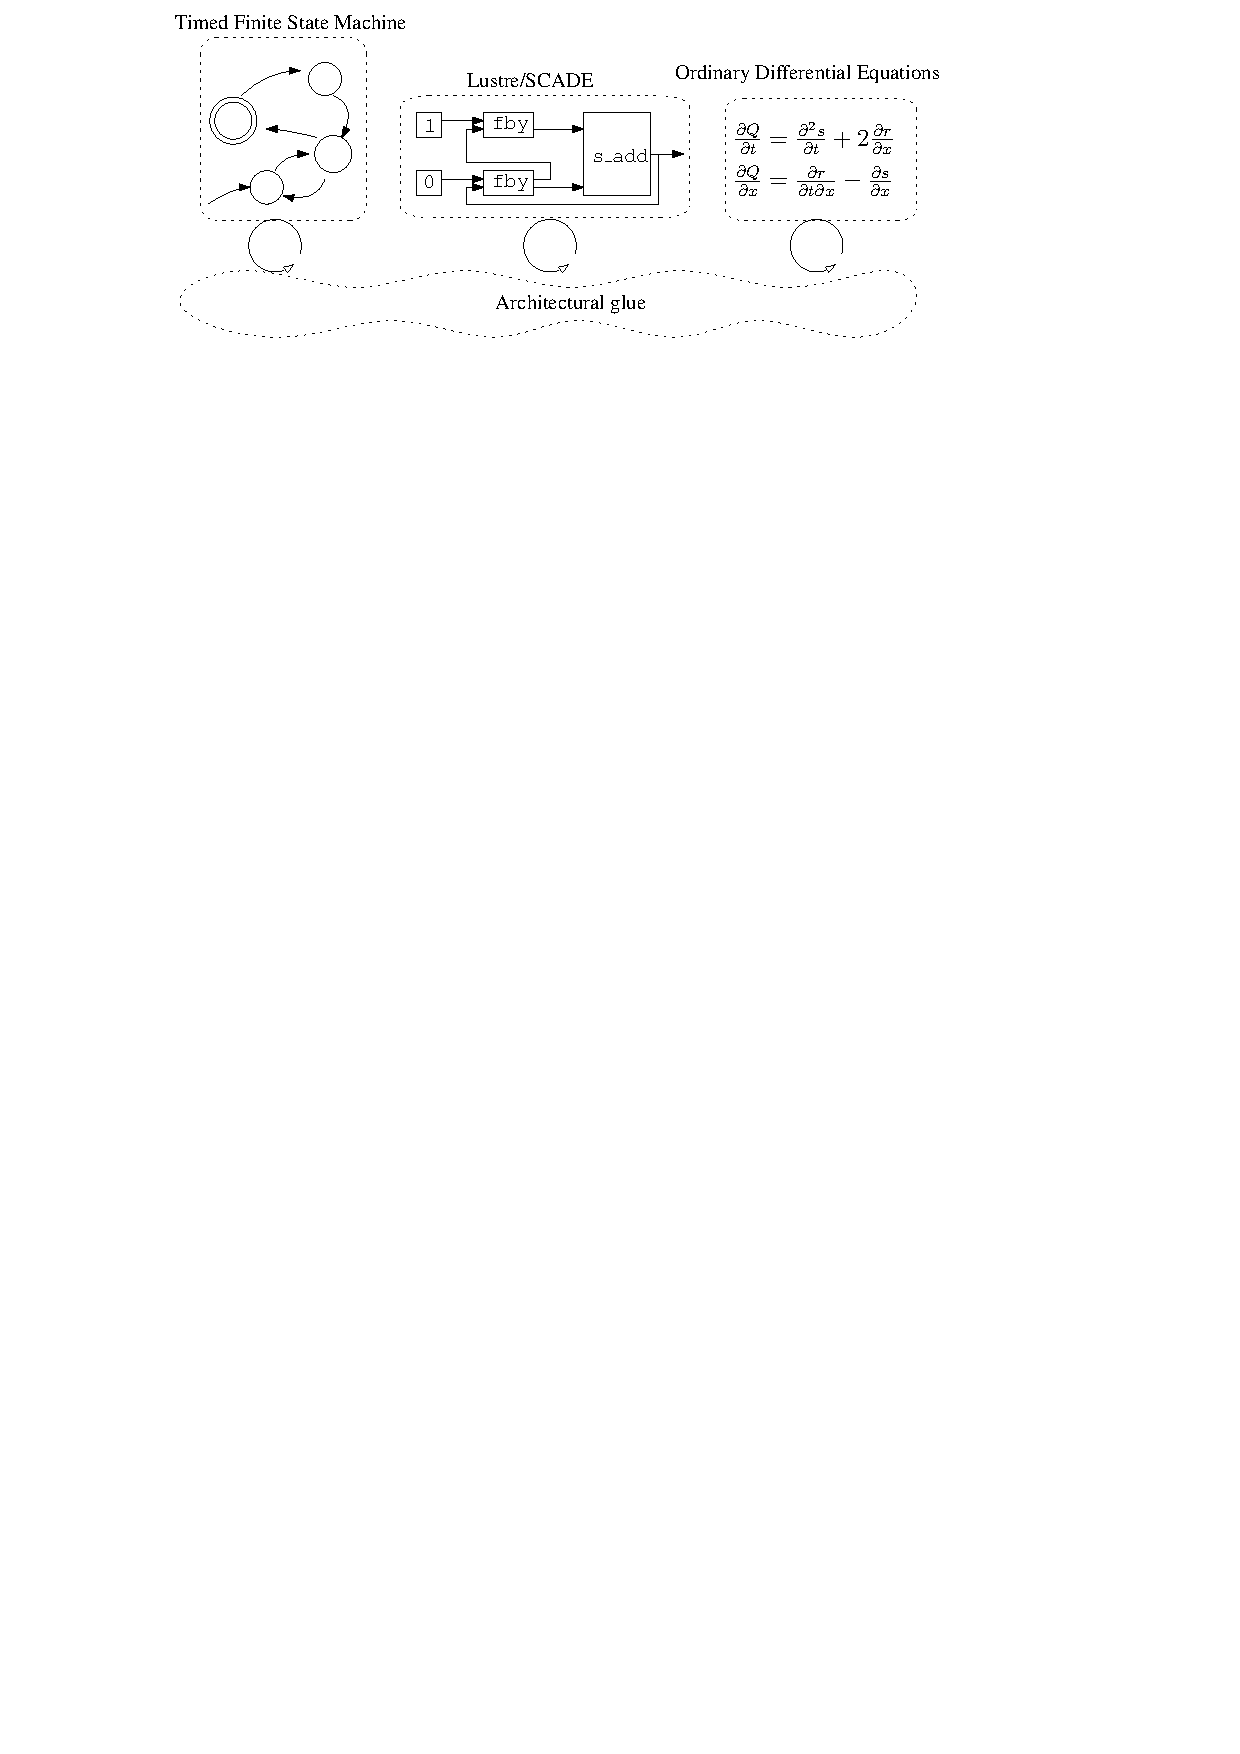
\includegraphics{glue.pdf}
 \caption{A Heterogeneous Timed System Model}
 \label{fig:het-timed-system}
\end{figure}%
\end{isamarkuptext}\isamarkuptrue%
%
\begin{isamarkuptext}%
In order to tackle the heterogeneous nature of the subsystems, we abstract their behavior as clocks. 
Each clock models an event, i.e., something that can occur or not at a given time. This time is measured 
in a time frame associated with each clock, and the nature of time (integer, rational, real, or any 
type with a linear order) is specific to each clock. 
When the event associated with a clock occurs, the clock ticks. In order to support any kind of 
behavior for the subsystems, we are only interested in specifying what we can observe at a series 
of discrete instants. There are two constraints on observations: a clock may tick only at an 
observation instant, and the time on any clock cannot decrease from an instant to the next one. 
However, it is always possible to add arbitrary observation instants, which allows for stuttering 
and modular composition of systems. 
As a consequence, the key concept of our setting is the notion of a clock-indexed Kripke model: 
\isa{{\isasymSigma}\isactrlsup {\isasyminfinity}\ {\isacharequal}\ {\isasymnat}\ {\isasymrightarrow}\ {\isasymK}\ {\isasymrightarrow}\ {\isacharparenleft}{\isasymbool}\ {\isasymtimes}\ {\isasymT}{\isacharparenright}}, where \isa{{\isasymK}} is an enumerable set of clocks, \isa{{\isasymbool}} 
is the set of booleans – used to  indicate that a clock ticks at a given instant – and \isa{{\isasymT}} 
is a universal metric time space for which we only assume that it is large enough to contain all 
individual time spaces of clocks and that it is ordered by some linear ordering \isa{{\isacharparenleft}{\isasymle}\isactrlsub {\isasymT}{\isacharparenright}}.%
\end{isamarkuptext}\isamarkuptrue%
%
\begin{isamarkuptext}%
The elements of \isa{{\isasymSigma}\isactrlsup {\isasyminfinity}} are called runs. A specification language is a set of 
  operators that constrains the set of possible monotonic runs. Specifications are composed by 
  intersecting the denoted run sets of constraint operators.
  Consequently, such specification languages do not limit the number of clocks used to model a 
  system (as long as it is finite) and it is always possible to add clocks to a specification. 
  Moreover, they are \emph{compositional} by construction since the composition of specifications 
  consists of the conjunction of their constraints.%
\end{isamarkuptext}\isamarkuptrue%
%
\begin{isamarkuptext}%
This work provides the following contributions:

%
\begin{itemize}%
\item defining the non-trivial language \isa{TESL\isactrlsup {\isacharasterisk}} in terms of clock-indexed Kripke models, 

\item proving that this denotational semantics is stuttering invariant,

\item defining an adapted form of symbolic primitives and presenting the set of operational 
semantic rules,

\item presenting formal proofs for soundness, completeness, and progress of the latter.%
\end{itemize}%
\end{isamarkuptext}\isamarkuptrue%
%
\isadelimdocument
%
\endisadelimdocument
%
\isatagdocument
%
\isamarkupsection{The TESL Language%
}
\isamarkuptrue%
%
\endisatagdocument
{\isafolddocument}%
%
\isadelimdocument
%
\endisadelimdocument
%
\begin{isamarkuptext}%
The TESL language \cite{BouJacHarPro2014MEMOCODE} was initially designed to coordinate the
  execution of heterogeneous components during the simulation of a system. We define here a minimal
  kernel of operators that will form the basis of a family of specification languages, including the
  original TESL language, which is described at \url{http://wdi.supelec.fr/software/TESL/}.%
\end{isamarkuptext}\isamarkuptrue%
%
\isadelimdocument
%
\endisadelimdocument
%
\isatagdocument
%
\isamarkupsubsection{Instantaneous Causal Operators%
}
\isamarkuptrue%
%
\endisatagdocument
{\isafolddocument}%
%
\isadelimdocument
%
\endisadelimdocument
%
\begin{isamarkuptext}%
TESL has operators to deal with instantaneous causality, i.e., to react to an event occurrence
in the very same observation instant.

%
\begin{itemize}%
\item \isatt{c1\ implies\ c2} means that at any instant where \isatt{c1} ticks, \isatt{c2} has to tick too.

\item \isatt{c1\ implies\ not\ c2} means that at any instant where \isatt{c1} ticks, \isatt{c2} cannot tick.

\item \isatt{c1\ kills\ c2} means that at any instant where \isatt{c1} ticks, and at any future instant, 
\isatt{c2} cannot tick.%
\end{itemize}%
\end{isamarkuptext}\isamarkuptrue%
%
\isadelimdocument
%
\endisadelimdocument
%
\isatagdocument
%
\isamarkupsubsection{Temporal Operators%
}
\isamarkuptrue%
%
\endisatagdocument
{\isafolddocument}%
%
\isadelimdocument
%
\endisadelimdocument
%
\begin{isamarkuptext}%
TESL also has chronometric temporal operators that deal with dates and chronometric delays.

%
\begin{itemize}%
\item \isatt{c\ sporadic\ t} means that clock \isatt{c} must have a tick at time \isatt{t} on its own time scale.

\item \isatt{c1\ sporadic\ t\ on\ c2} means that clock \isatt{c1} must have a tick at an instant where the time 
on \isatt{c2} is \isatt{t}.

\item \isatt{c1\ time\ delayed\ by\ d\ on\ m\ implies\ c2} means that every time clock \isatt{c1} ticks, \isatt{c2} must have 
a tick at the first instant where the time on \isatt{m} is \isatt{d} later than it was when \isatt{c1} had ticked.
This means that every tick on \isatt{c1} is followed by a tick on \isatt{c2} after a delay \isatt{d} measured
on the time scale of clock \isatt{m}.

\item \isatt{time\ relation\ (c1{\char`\,}\ c2)\ in\ R} means that at every instant, the current time on clocks \isatt{c1}
and \isatt{c2} must be in relation \isatt{R}. By default, the time lines of different clocks are 
independent. This operator allows us to link two time lines, for instance to model the fact
that time in a GPS satellite and time in a GPS receiver on Earth are not the same but are 
related. Time being polymorphic in TESL, this can also be used to model the fact that the
angular position on the camshaft of an engine moves twice as fast as the angular position 
on the crankshaft~\footnote{See \url{http://wdi.supelec.fr/software/TESL/GalleryEngine} for more details}. 
We may consider only linear arithmetic relations to restrict the problem to a domain where 
the resolution is decidable.%
\end{itemize}%
\end{isamarkuptext}\isamarkuptrue%
%
\isadelimdocument
%
\endisadelimdocument
%
\isatagdocument
%
\isamarkupsubsection{Asynchronous Operators%
}
\isamarkuptrue%
%
\endisatagdocument
{\isafolddocument}%
%
\isadelimdocument
%
\endisadelimdocument
%
\begin{isamarkuptext}%
The last category of TESL operators allows the specification of asynchronous relations between
event occurrences. They do not specify the precise instants at which ticks have to occur, 
they only put bounds on the set of instants at which they should occur.

%
\begin{itemize}%
\item \isatt{c1\ weakly\ precedes\ c2} means that for each tick on \isatt{c2}, there must be at least one tick
on \isatt{c1} at a previous or at the same instant. This can also be expressed by stating
that at each instant, the number of ticks since the beginning of the run must be lower or 
equal on \isatt{c2} than on \isatt{c1}.

\item \isatt{c1\ strictly\ precedes\ c2} means that for each tick on \isatt{c2}, there must be at least one tick
on \isatt{c1} at a previous instant. This can also be expressed by saying that at each instant, 
the number of ticks on \isatt{c2} from the beginning of the run to this instant, must be lower or 
equal to the number of ticks on \isatt{c1} from the beginning of the run to the previous instant.%
\end{itemize}%
\end{isamarkuptext}\isamarkuptrue%
%
\isadelimtheory
%
\endisadelimtheory
%
\isatagtheory
%
\endisatagtheory
{\isafoldtheory}%
%
\isadelimtheory
%
\endisadelimtheory
%
\end{isabellebody}%
\endinput
%:%file=~/Documents/Recherche/Thesards/2014_Hai_NGUYEN_VAN/Heron_git/reiher2/TESL_Fred/src/Introduction.thy%:%
%:%11=1%:%
%:%41=10%:%
%:%53=12%:%
%:%54=13%:%
%:%55=14%:%
%:%56=15%:%
%:%57=16%:%
%:%58=17%:%
%:%59=18%:%
%:%60=19%:%
%:%62=21%:%
%:%63=22%:%
%:%67=23%:%
%:%68=24%:%
%:%70=25%:%
%:%71=26%:%
%:%73=27%:%
%:%74=28%:%
%:%76=29%:%
%:%77=30%:%
%:%78=31%:%
%:%80=32%:%
%:%81=33%:%
%:%83=34%:%
%:%84=35%:%
%:%89=39%:%
%:%90=40%:%
%:%91=41%:%
%:%92=42%:%
%:%93=43%:%
%:%94=44%:%
%:%98=66%:%
%:%99=67%:%
%:%100=68%:%
%:%101=69%:%
%:%102=70%:%
%:%103=71%:%
%:%104=72%:%
%:%105=73%:%
%:%106=74%:%
%:%107=75%:%
%:%108=76%:%
%:%109=77%:%
%:%110=78%:%
%:%111=79%:%
%:%112=80%:%
%:%116=84%:%
%:%117=85%:%
%:%118=86%:%
%:%119=87%:%
%:%120=88%:%
%:%121=89%:%
%:%122=90%:%
%:%126=94%:%
%:%130=95%:%
%:%132=96%:%
%:%134=97%:%
%:%135=98%:%
%:%137=99%:%
%:%147=102%:%
%:%159=105%:%
%:%160=106%:%
%:%161=107%:%
%:%162=108%:%
%:%171=111%:%
%:%183=113%:%
%:%184=114%:%
%:%188=115%:%
%:%190=116%:%
%:%192=117%:%
%:%193=118%:%
%:%203=121%:%
%:%215=123%:%
%:%219=124%:%
%:%221=125%:%
%:%222=126%:%
%:%224=127%:%
%:%225=128%:%
%:%226=129%:%
%:%227=130%:%
%:%229=131%:%
%:%230=132%:%
%:%231=133%:%
%:%232=134%:%
%:%233=135%:%
%:%234=136%:%
%:%235=137%:%
%:%236=138%:%
%:%237=139%:%
%:%247=141%:%
%:%259=143%:%
%:%260=144%:%
%:%261=145%:%
%:%265=146%:%
%:%266=147%:%
%:%267=148%:%
%:%268=149%:%
%:%270=150%:%
%:%271=151%:%
%:%272=152%:%
%:%273=153%:%

%
\begin{isabellebody}%
\setisabellecontext{TESL}%
%
\begin{isamarkuptext}%
\chapter[Core TESL: Syntax and Basics]{The Core of the TESL Language: Syntax and Basics}%
\end{isamarkuptext}\isamarkuptrue%
%
\isadelimtheory
%
\endisadelimtheory
%
\isatagtheory
\isacommand{theory}\isamarkupfalse%
\ TESL\isanewline
\isakeyword{imports}\ Main\isanewline
\isanewline
\isakeyword{begin}%
\endisatagtheory
{\isafoldtheory}%
%
\isadelimtheory
%
\endisadelimtheory
%
\isadelimdocument
%
\endisadelimdocument
%
\isatagdocument
%
\isamarkupsection{Syntactic Representation%
}
\isamarkuptrue%
%
\endisatagdocument
{\isafolddocument}%
%
\isadelimdocument
%
\endisadelimdocument
%
\begin{isamarkuptext}%
We define here the syntax of TESL specifications.%
\end{isamarkuptext}\isamarkuptrue%
%
\isadelimdocument
%
\endisadelimdocument
%
\isatagdocument
%
\isamarkupsubsection{Basic elements of a specification%
}
\isamarkuptrue%
%
\endisatagdocument
{\isafolddocument}%
%
\isadelimdocument
%
\endisadelimdocument
%
\begin{isamarkuptext}%
The following items appear in specifications:

%
\begin{itemize}%
\item Clocks, which are identified by a name.

\item Tag constants are just constants of a type which denotes the metric time space.%
\end{itemize}%
\end{isamarkuptext}\isamarkuptrue%
\isacommand{datatype}\isamarkupfalse%
\ \ \ \ \ clock\ \ \ \ \ \ \ \ \ {\isacharequal}\ Clk\ {\isacartoucheopen}string{\isacartoucheclose}\isanewline
\isacommand{type{\isacharunderscore}synonym}\isamarkupfalse%
\ instant{\isacharunderscore}index\ {\isacharequal}\ {\isacartoucheopen}nat{\isacartoucheclose}\isanewline
\isanewline
\isacommand{datatype}\isamarkupfalse%
\ \ \ \ \ {\isacharprime}{\isasymtau}\ tag{\isacharunderscore}const\ {\isacharequal}\ \ TConst\ \ \ {\isacharparenleft}the{\isacharunderscore}tag{\isacharunderscore}const\ {\isacharcolon}\ {\isacharprime}{\isasymtau}{\isacharparenright}\ \ \ \ \ \ \ \ \ {\isacharparenleft}{\isacartoucheopen}{\isasymtau}\isactrlsub c\isactrlsub s\isactrlsub t{\isacartoucheclose}{\isacharparenright}%
\isadelimdocument
%
\endisadelimdocument
%
\isatagdocument
%
\isamarkupsubsection{Operators for the TESL language%
}
\isamarkuptrue%
%
\endisatagdocument
{\isafolddocument}%
%
\isadelimdocument
%
\endisadelimdocument
%
\begin{isamarkuptext}%
The type of atomic TESL constraints, which can be combined to form specifications.%
\end{isamarkuptext}\isamarkuptrue%
\isacommand{datatype}\isamarkupfalse%
\ {\isacharprime}{\isasymtau}\ TESL{\isacharunderscore}atomic\ {\isacharequal}\isanewline
\ \ \ \ SporadicOn\ \ \ \ \ \ \ {\isacartoucheopen}clock{\isacartoucheclose}\ {\isacartoucheopen}{\isacharprime}{\isasymtau}\ tag{\isacharunderscore}const{\isacartoucheclose}\ \ {\isacartoucheopen}clock{\isacartoucheclose}\ \ {\isacharparenleft}{\isacartoucheopen}{\isacharunderscore}\ sporadic\ {\isacharunderscore}\ on\ {\isacharunderscore}{\isacartoucheclose}\ {\isadigit{5}}{\isadigit{5}}{\isacharparenright}\isanewline
\ \ {\isacharbar}\ TagRelation\ \ \ \ \ \ {\isacartoucheopen}clock{\isacartoucheclose}\ {\isacartoucheopen}clock{\isacartoucheclose}\ {\isacartoucheopen}{\isacharparenleft}{\isacharprime}{\isasymtau}\ tag{\isacharunderscore}const\ {\isasymtimes}\ {\isacharprime}{\isasymtau}\ tag{\isacharunderscore}const{\isacharparenright}\ {\isasymRightarrow}\ bool{\isacartoucheclose}\ \isanewline
\ \ \ \ \ \ \ \ \ \ \ \ \ \ \ \ \ \ \ \ \ \ \ \ \ \ \ \ \ \ \ \ \ \ \ \ \ \ \ \ \ \ \ \ \ \ \ \ \ \ \ \ \ \ {\isacharparenleft}{\isacartoucheopen}time{\isacharminus}relation\ {\isasymlfloor}{\isacharunderscore}{\isacharcomma}\ {\isacharunderscore}{\isasymrfloor}\ {\isasymin}\ {\isacharunderscore}{\isacartoucheclose}\ {\isadigit{5}}{\isadigit{5}}{\isacharparenright}\isanewline
\ \ {\isacharbar}\ Implies\ \ \ \ \ \ \ \ \ \ {\isacartoucheopen}clock{\isacartoucheclose}\ {\isacartoucheopen}clock{\isacartoucheclose}\ \ \ \ \ \ \ \ \ \ \ \ \ \ \ \ \ \ {\isacharparenleft}\isakeyword{infixr}\ {\isacartoucheopen}implies{\isacartoucheclose}\ {\isadigit{5}}{\isadigit{5}}{\isacharparenright}\isanewline
\ \ {\isacharbar}\ ImpliesNot\ \ \ \ \ \ \ {\isacartoucheopen}clock{\isacartoucheclose}\ {\isacartoucheopen}clock{\isacartoucheclose}\ \ \ \ \ \ \ \ \ \ \ \ \ \ \ \ \ \ {\isacharparenleft}\isakeyword{infixr}\ {\isacartoucheopen}implies\ not{\isacartoucheclose}\ {\isadigit{5}}{\isadigit{5}}{\isacharparenright}\isanewline
\ \ {\isacharbar}\ TimeDelayedBy\ \ \ \ {\isacartoucheopen}clock{\isacartoucheclose}\ {\isacartoucheopen}{\isacharprime}{\isasymtau}\ tag{\isacharunderscore}const{\isacartoucheclose}\ {\isacartoucheopen}clock{\isacartoucheclose}\ {\isacartoucheopen}clock{\isacartoucheclose}\ \isanewline
\ \ \ \ \ \ \ \ \ \ \ \ \ \ \ \ \ \ \ \ \ \ \ \ \ \ \ \ \ \ \ \ \ \ \ \ \ \ \ \ \ \ \ \ \ \ \ \ \ \ \ \ \ \ {\isacharparenleft}{\isacartoucheopen}{\isacharunderscore}\ time{\isacharminus}delayed\ by\ {\isacharunderscore}\ on\ {\isacharunderscore}\ implies\ {\isacharunderscore}{\isacartoucheclose}\ {\isadigit{5}}{\isadigit{5}}{\isacharparenright}\isanewline
\ \ {\isacharbar}\ DelayedBy\ \ \ \ \ \ \ \ {\isacartoucheopen}clock{\isacartoucheclose}\ {\isacartoucheopen}nat{\isacartoucheclose}\ {\isacartoucheopen}clock{\isacartoucheclose}\ {\isacartoucheopen}clock{\isacartoucheclose}\ \isanewline
\ \ \ \ \ \ \ \ \ \ \ \ \ \ \ \ \ \ \ \ \ \ \ \ \ \ \ \ \ \ \ \ \ \ \ \ \ \ \ \ \ \ \ \ \ \ \ \ \ \ \ \ \ \ {\isacharparenleft}{\isacartoucheopen}{\isacharunderscore}\ delayed\ by\ {\isacharunderscore}\ on\ {\isacharunderscore}\ implies\ {\isacharunderscore}{\isacartoucheclose}\ {\isadigit{5}}{\isadigit{5}}{\isacharparenright}\isanewline
\ \ {\isacharbar}\ WeaklyPrecedes\ \ \ {\isacartoucheopen}clock{\isacartoucheclose}\ {\isacartoucheopen}clock{\isacartoucheclose}\ \ \ \ \ \ \ \ \ \ \ \ \ \ \ \ \ \ {\isacharparenleft}\isakeyword{infixr}\ {\isacartoucheopen}weakly\ precedes{\isacartoucheclose}\ {\isadigit{5}}{\isadigit{5}}{\isacharparenright}\isanewline
\ \ {\isacharbar}\ StrictlyPrecedes\ {\isacartoucheopen}clock{\isacartoucheclose}\ {\isacartoucheopen}clock{\isacartoucheclose}\ \ \ \ \ \ \ \ \ \ \ \ \ \ \ \ \ \ {\isacharparenleft}\isakeyword{infixr}\ {\isacartoucheopen}strictly\ precedes{\isacartoucheclose}\ {\isadigit{5}}{\isadigit{5}}{\isacharparenright}\isanewline
\ \ {\isacharbar}\ Kills\ \ \ \ \ \ \ \ \ \ \ \ {\isacartoucheopen}clock{\isacartoucheclose}\ {\isacartoucheopen}clock{\isacartoucheclose}\ \ \ \ \ \ \ \ \ \ \ \ \ \ \ \ \ \ {\isacharparenleft}\isakeyword{infixr}\ {\isacartoucheopen}kills{\isacartoucheclose}\ {\isadigit{5}}{\isadigit{5}}{\isacharparenright}\isanewline
\ \ %
\isamarkupcmt{State storing constraints for implementing top level constraints%
}\isanewline
\ \ {\isacharbar}\ DelayCount\ \ \ \ \ \ \ {\isacartoucheopen}nat{\isacartoucheclose}\ {\isacartoucheopen}nat{\isacartoucheclose}\ {\isacartoucheopen}clock{\isacartoucheclose}\ {\isacartoucheopen}clock{\isacartoucheclose}\ \ \ \ \ \ {\isacharparenleft}{\isacartoucheopen}from\ {\isacharunderscore}\ delay\ count\ {\isacharunderscore}\ on\ {\isacharunderscore}\ implies\ {\isacharunderscore}{\isacartoucheclose}\ {\isadigit{5}}{\isadigit{5}}{\isacharparenright}\isanewline
\isanewline
\isacommand{fun}\isamarkupfalse%
\ spec{\isacharunderscore}atom\isanewline
\isakeyword{where}\isanewline
\ \ {\isacartoucheopen}spec{\isacharunderscore}atom\ {\isacharparenleft}DelayCount\ m\ n\ c{\isadigit{1}}\ c{\isadigit{2}}{\isacharparenright}\ {\isacharequal}\ False{\isacartoucheclose}\isanewline
{\isacharbar}\ {\isacartoucheopen}spec{\isacharunderscore}atom\ {\isacharunderscore}\ {\isacharequal}\ True{\isacartoucheclose}\isanewline
\isanewline
\isacommand{primrec}\isamarkupfalse%
\ spec{\isacharunderscore}formula\isanewline
\isakeyword{where}\isanewline
\ \ {\isacartoucheopen}spec{\isacharunderscore}formula\ {\isacharbrackleft}{\isacharbrackright}\ {\isacharequal}\ True{\isacartoucheclose}\isanewline
{\isacharbar}\ {\isacartoucheopen}spec{\isacharunderscore}formula\ {\isacharparenleft}{\isasymphi}\ {\isacharhash}\ S{\isacharparenright}\ {\isacharequal}\ {\isacharparenleft}spec{\isacharunderscore}atom\ {\isasymphi}\ {\isasymand}\ spec{\isacharunderscore}formula\ S{\isacharparenright}{\isacartoucheclose}%
\begin{isamarkuptext}%
A TESL formula is just a list of atomic constraints, with implicit conjunction
  for the semantics.%
\end{isamarkuptext}\isamarkuptrue%
\isacommand{type{\isacharunderscore}synonym}\isamarkupfalse%
\ {\isacharprime}{\isasymtau}\ TESL{\isacharunderscore}formula\ {\isacharequal}\ {\isacartoucheopen}{\isacharprime}{\isasymtau}\ TESL{\isacharunderscore}atomic\ list{\isacartoucheclose}%
\begin{isamarkuptext}%
We call \emph{positive atoms} the atomic constraints that create ticks from nothing.
  Only sporadic constraints are positive in the current version of TESL.%
\end{isamarkuptext}\isamarkuptrue%
\isacommand{fun}\isamarkupfalse%
\ positive{\isacharunderscore}atom\ {\isacharcolon}{\isacharcolon}\ {\isacartoucheopen}{\isacharprime}{\isasymtau}\ TESL{\isacharunderscore}atomic\ {\isasymRightarrow}\ bool{\isacartoucheclose}\ \isakeyword{where}\isanewline
\ \ \ \ {\isacartoucheopen}positive{\isacharunderscore}atom\ {\isacharparenleft}{\isacharunderscore}\ sporadic\ {\isacharunderscore}\ on\ {\isacharunderscore}{\isacharparenright}\ {\isacharequal}\ True{\isacartoucheclose}\isanewline
\ \ {\isacharbar}\ {\isacartoucheopen}positive{\isacharunderscore}atom\ {\isacharunderscore}\ \ \ \ \ \ \ \ \ \ \ \ \ \ \ \ \ \ \ {\isacharequal}\ False{\isacartoucheclose}%
\begin{isamarkuptext}%
The \isa{NoSporadic} function removes sporadic constraints from a TESL formula.%
\end{isamarkuptext}\isamarkuptrue%
\isacommand{abbreviation}\isamarkupfalse%
\ NoSporadic\ {\isacharcolon}{\isacharcolon}\ {\isacartoucheopen}{\isacharprime}{\isasymtau}\ TESL{\isacharunderscore}formula\ {\isasymRightarrow}\ {\isacharprime}{\isasymtau}\ TESL{\isacharunderscore}formula{\isacartoucheclose}\isanewline
\isakeyword{where}\ \isanewline
\ \ {\isacartoucheopen}NoSporadic\ f\ {\isasymequiv}\ {\isacharparenleft}List{\isachardot}filter\ {\isacharparenleft}{\isasymlambda}f\isactrlsub a\isactrlsub t\isactrlsub o\isactrlsub m{\isachardot}\ case\ f\isactrlsub a\isactrlsub t\isactrlsub o\isactrlsub m\ of\isanewline
\ \ \ \ \ \ {\isacharunderscore}\ sporadic\ {\isacharunderscore}\ on\ {\isacharunderscore}\ {\isasymRightarrow}\ False\isanewline
\ \ \ \ {\isacharbar}\ {\isacharunderscore}\ {\isasymRightarrow}\ True{\isacharparenright}\ f{\isacharparenright}{\isacartoucheclose}%
\isadelimdocument
%
\endisadelimdocument
%
\isatagdocument
%
\isamarkupsubsection{Field Structure of the Metric Time Space%
}
\isamarkuptrue%
%
\endisatagdocument
{\isafolddocument}%
%
\isadelimdocument
%
\endisadelimdocument
%
\begin{isamarkuptext}%
In order to handle tag relations and delays, tags must belong to a field.
  We show here that this is the case when the type parameter of \isa{{\isacharprime}{\isasymtau}\ tag{\isacharunderscore}const} 
  is itself a field.%
\end{isamarkuptext}\isamarkuptrue%
\isacommand{instantiation}\isamarkupfalse%
\ tag{\isacharunderscore}const\ {\isacharcolon}{\isacharcolon}{\isacharparenleft}field{\isacharparenright}field\isanewline
\isakeyword{begin}\isanewline
\ \ \isacommand{fun}\isamarkupfalse%
\ inverse{\isacharunderscore}tag{\isacharunderscore}const\isanewline
\ \ \isakeyword{where}\ {\isacartoucheopen}inverse\ {\isacharparenleft}{\isasymtau}\isactrlsub c\isactrlsub s\isactrlsub t\ t{\isacharparenright}\ {\isacharequal}\ {\isasymtau}\isactrlsub c\isactrlsub s\isactrlsub t\ {\isacharparenleft}inverse\ t{\isacharparenright}{\isacartoucheclose}\isanewline
\isanewline
\ \ \isacommand{fun}\isamarkupfalse%
\ divide{\isacharunderscore}tag{\isacharunderscore}const\ \isanewline
\ \ \ \ \isakeyword{where}\ {\isacartoucheopen}divide\ {\isacharparenleft}{\isasymtau}\isactrlsub c\isactrlsub s\isactrlsub t\ t\isactrlsub {\isadigit{1}}{\isacharparenright}\ {\isacharparenleft}{\isasymtau}\isactrlsub c\isactrlsub s\isactrlsub t\ t\isactrlsub {\isadigit{2}}{\isacharparenright}\ {\isacharequal}\ {\isasymtau}\isactrlsub c\isactrlsub s\isactrlsub t\ {\isacharparenleft}divide\ t\isactrlsub {\isadigit{1}}\ t\isactrlsub {\isadigit{2}}{\isacharparenright}{\isacartoucheclose}\isanewline
\isanewline
\ \ \isacommand{fun}\isamarkupfalse%
\ uminus{\isacharunderscore}tag{\isacharunderscore}const\isanewline
\ \ \ \ \isakeyword{where}\ {\isacartoucheopen}uminus\ {\isacharparenleft}{\isasymtau}\isactrlsub c\isactrlsub s\isactrlsub t\ t{\isacharparenright}\ {\isacharequal}\ {\isasymtau}\isactrlsub c\isactrlsub s\isactrlsub t\ {\isacharparenleft}uminus\ t{\isacharparenright}{\isacartoucheclose}\isanewline
\isanewline
\isacommand{fun}\isamarkupfalse%
\ minus{\isacharunderscore}tag{\isacharunderscore}const\isanewline
\ \ \isakeyword{where}\ {\isacartoucheopen}minus\ {\isacharparenleft}{\isasymtau}\isactrlsub c\isactrlsub s\isactrlsub t\ t\isactrlsub {\isadigit{1}}{\isacharparenright}\ {\isacharparenleft}{\isasymtau}\isactrlsub c\isactrlsub s\isactrlsub t\ t\isactrlsub {\isadigit{2}}{\isacharparenright}\ {\isacharequal}\ {\isasymtau}\isactrlsub c\isactrlsub s\isactrlsub t\ {\isacharparenleft}minus\ t\isactrlsub {\isadigit{1}}\ t\isactrlsub {\isadigit{2}}{\isacharparenright}{\isacartoucheclose}\isanewline
\isanewline
\isacommand{definition}\isamarkupfalse%
\ {\isacartoucheopen}one{\isacharunderscore}tag{\isacharunderscore}const\ {\isasymequiv}\ {\isasymtau}\isactrlsub c\isactrlsub s\isactrlsub t\ {\isadigit{1}}{\isacartoucheclose}\isanewline
\isanewline
\isacommand{fun}\isamarkupfalse%
\ times{\isacharunderscore}tag{\isacharunderscore}const\isanewline
\ \ \isakeyword{where}\ {\isacartoucheopen}times\ {\isacharparenleft}{\isasymtau}\isactrlsub c\isactrlsub s\isactrlsub t\ t\isactrlsub {\isadigit{1}}{\isacharparenright}\ {\isacharparenleft}{\isasymtau}\isactrlsub c\isactrlsub s\isactrlsub t\ t\isactrlsub {\isadigit{2}}{\isacharparenright}\ {\isacharequal}\ {\isasymtau}\isactrlsub c\isactrlsub s\isactrlsub t\ {\isacharparenleft}times\ t\isactrlsub {\isadigit{1}}\ t\isactrlsub {\isadigit{2}}{\isacharparenright}{\isacartoucheclose}\isanewline
\isanewline
\isacommand{definition}\isamarkupfalse%
\ {\isacartoucheopen}zero{\isacharunderscore}tag{\isacharunderscore}const\ {\isasymequiv}\ {\isasymtau}\isactrlsub c\isactrlsub s\isactrlsub t\ {\isadigit{0}}{\isacartoucheclose}\isanewline
\isanewline
\isacommand{fun}\isamarkupfalse%
\ plus{\isacharunderscore}tag{\isacharunderscore}const\isanewline
\ \ \isakeyword{where}\ {\isacartoucheopen}plus\ {\isacharparenleft}{\isasymtau}\isactrlsub c\isactrlsub s\isactrlsub t\ t\isactrlsub {\isadigit{1}}{\isacharparenright}\ {\isacharparenleft}{\isasymtau}\isactrlsub c\isactrlsub s\isactrlsub t\ t\isactrlsub {\isadigit{2}}{\isacharparenright}\ {\isacharequal}\ {\isasymtau}\isactrlsub c\isactrlsub s\isactrlsub t\ {\isacharparenleft}plus\ t\isactrlsub {\isadigit{1}}\ t\isactrlsub {\isadigit{2}}{\isacharparenright}{\isacartoucheclose}\isanewline
\isanewline
\isacommand{instance}\isamarkupfalse%
%
\isadelimproof
\ %
\endisadelimproof
%
\isatagproof
\isacommand{proof}\isamarkupfalse%
%
\begin{isamarkuptext}%
Multiplication is associative.%
\end{isamarkuptext}\isamarkuptrue%
\ \ \isacommand{fix}\isamarkupfalse%
\ a{\isacharcolon}{\isacharcolon}{\isacartoucheopen}{\isacharprime}{\isasymtau}{\isacharcolon}{\isacharcolon}field\ tag{\isacharunderscore}const{\isacartoucheclose}\ \isakeyword{and}\ b{\isacharcolon}{\isacharcolon}{\isacartoucheopen}{\isacharprime}{\isasymtau}{\isacharcolon}{\isacharcolon}field\ tag{\isacharunderscore}const{\isacartoucheclose}\isanewline
\ \ \ \ \ \ \ \ \ \ \ \ \ \ \ \ \ \ \ \ \ \ \ \ \ \ \ \ \ \ \ \isakeyword{and}\ c{\isacharcolon}{\isacharcolon}{\isacartoucheopen}{\isacharprime}{\isasymtau}{\isacharcolon}{\isacharcolon}field\ tag{\isacharunderscore}const{\isacartoucheclose}\isanewline
\ \ \isacommand{obtain}\isamarkupfalse%
\ u\ v\ w\ \isakeyword{where}\ {\isacartoucheopen}a\ {\isacharequal}\ {\isasymtau}\isactrlsub c\isactrlsub s\isactrlsub t\ u{\isacartoucheclose}\ \isakeyword{and}\ {\isacartoucheopen}b\ {\isacharequal}\ {\isasymtau}\isactrlsub c\isactrlsub s\isactrlsub t\ v{\isacartoucheclose}\ \isakeyword{and}\ {\isacartoucheopen}c\ {\isacharequal}\ {\isasymtau}\isactrlsub c\isactrlsub s\isactrlsub t\ w{\isacartoucheclose}\isanewline
\ \ \ \ \isacommand{using}\isamarkupfalse%
\ tag{\isacharunderscore}const{\isachardot}exhaust\ \isacommand{by}\isamarkupfalse%
\ metis\isanewline
\ \ \isacommand{thus}\isamarkupfalse%
\ {\isacartoucheopen}a\ {\isacharasterisk}\ b\ {\isacharasterisk}\ c\ {\isacharequal}\ a\ {\isacharasterisk}\ {\isacharparenleft}b\ {\isacharasterisk}\ c{\isacharparenright}{\isacartoucheclose}\isanewline
\ \ \ \ \isacommand{by}\isamarkupfalse%
\ {\isacharparenleft}simp\ add{\isacharcolon}\ TESL{\isachardot}times{\isacharunderscore}tag{\isacharunderscore}const{\isachardot}simps{\isacharparenright}\isanewline
\isacommand{next}\isamarkupfalse%
%
\begin{isamarkuptext}%
Multiplication is commutative.%
\end{isamarkuptext}\isamarkuptrue%
\ \ \isacommand{fix}\isamarkupfalse%
\ a{\isacharcolon}{\isacharcolon}{\isacartoucheopen}{\isacharprime}{\isasymtau}{\isacharcolon}{\isacharcolon}field\ tag{\isacharunderscore}const{\isacartoucheclose}\ \isakeyword{and}\ b{\isacharcolon}{\isacharcolon}{\isacartoucheopen}{\isacharprime}{\isasymtau}{\isacharcolon}{\isacharcolon}field\ tag{\isacharunderscore}const{\isacartoucheclose}\isanewline
\ \ \isacommand{obtain}\isamarkupfalse%
\ u\ v\ \isakeyword{where}\ {\isacartoucheopen}a\ {\isacharequal}\ {\isasymtau}\isactrlsub c\isactrlsub s\isactrlsub t\ u{\isacartoucheclose}\ \isakeyword{and}\ {\isacartoucheopen}b\ {\isacharequal}\ {\isasymtau}\isactrlsub c\isactrlsub s\isactrlsub t\ v{\isacartoucheclose}\ \isacommand{using}\isamarkupfalse%
\ tag{\isacharunderscore}const{\isachardot}exhaust\ \isacommand{by}\isamarkupfalse%
\ metis\isanewline
\ \ \isacommand{thus}\isamarkupfalse%
\ {\isacartoucheopen}\ a\ {\isacharasterisk}\ b\ {\isacharequal}\ b\ {\isacharasterisk}\ a{\isacartoucheclose}\isanewline
\ \ \ \ \isacommand{by}\isamarkupfalse%
\ {\isacharparenleft}simp\ add{\isacharcolon}\ TESL{\isachardot}times{\isacharunderscore}tag{\isacharunderscore}const{\isachardot}simps{\isacharparenright}\isanewline
\isacommand{next}\isamarkupfalse%
%
\begin{isamarkuptext}%
One is neutral for multiplication.%
\end{isamarkuptext}\isamarkuptrue%
\ \ \isacommand{fix}\isamarkupfalse%
\ a{\isacharcolon}{\isacharcolon}{\isacartoucheopen}{\isacharprime}{\isasymtau}{\isacharcolon}{\isacharcolon}field\ tag{\isacharunderscore}const{\isacartoucheclose}\isanewline
\ \ \isacommand{obtain}\isamarkupfalse%
\ u\ \isakeyword{where}\ {\isacartoucheopen}a\ {\isacharequal}\ {\isasymtau}\isactrlsub c\isactrlsub s\isactrlsub t\ u{\isacartoucheclose}\ \isacommand{using}\isamarkupfalse%
\ tag{\isacharunderscore}const{\isachardot}exhaust\ \isacommand{by}\isamarkupfalse%
\ blast\isanewline
\ \ \isacommand{thus}\isamarkupfalse%
\ {\isacartoucheopen}{\isadigit{1}}\ {\isacharasterisk}\ a\ {\isacharequal}\ a{\isacartoucheclose}\isanewline
\ \ \ \ \isacommand{by}\isamarkupfalse%
\ {\isacharparenleft}simp\ add{\isacharcolon}\ TESL{\isachardot}times{\isacharunderscore}tag{\isacharunderscore}const{\isachardot}simps\ one{\isacharunderscore}tag{\isacharunderscore}const{\isacharunderscore}def{\isacharparenright}\isanewline
\isacommand{next}\isamarkupfalse%
%
\begin{isamarkuptext}%
Addition is associative.%
\end{isamarkuptext}\isamarkuptrue%
\ \ \isacommand{fix}\isamarkupfalse%
\ a{\isacharcolon}{\isacharcolon}{\isacartoucheopen}{\isacharprime}{\isasymtau}{\isacharcolon}{\isacharcolon}field\ tag{\isacharunderscore}const{\isacartoucheclose}\ \isakeyword{and}\ b{\isacharcolon}{\isacharcolon}{\isacartoucheopen}{\isacharprime}{\isasymtau}{\isacharcolon}{\isacharcolon}field\ tag{\isacharunderscore}const{\isacartoucheclose}\isanewline
\ \ \ \ \ \ \ \ \ \ \ \ \ \ \ \ \ \ \ \ \ \ \ \ \ \ \ \ \ \ \ \isakeyword{and}\ c{\isacharcolon}{\isacharcolon}{\isacartoucheopen}{\isacharprime}{\isasymtau}{\isacharcolon}{\isacharcolon}field\ tag{\isacharunderscore}const{\isacartoucheclose}\isanewline
\ \ \isacommand{obtain}\isamarkupfalse%
\ u\ v\ w\ \isakeyword{where}\ {\isacartoucheopen}a\ {\isacharequal}\ {\isasymtau}\isactrlsub c\isactrlsub s\isactrlsub t\ u{\isacartoucheclose}\ \isakeyword{and}\ {\isacartoucheopen}b\ {\isacharequal}\ {\isasymtau}\isactrlsub c\isactrlsub s\isactrlsub t\ v{\isacartoucheclose}\ \isakeyword{and}\ {\isacartoucheopen}c\ {\isacharequal}\ {\isasymtau}\isactrlsub c\isactrlsub s\isactrlsub t\ w{\isacartoucheclose}\isanewline
\ \ \ \ \isacommand{using}\isamarkupfalse%
\ tag{\isacharunderscore}const{\isachardot}exhaust\ \isacommand{by}\isamarkupfalse%
\ metis\isanewline
\ \ \isacommand{thus}\isamarkupfalse%
\ {\isacartoucheopen}a\ {\isacharplus}\ b\ {\isacharplus}\ c\ {\isacharequal}\ a\ {\isacharplus}\ {\isacharparenleft}b\ {\isacharplus}\ c{\isacharparenright}{\isacartoucheclose}\isanewline
\ \ \ \ \isacommand{by}\isamarkupfalse%
\ {\isacharparenleft}simp\ add{\isacharcolon}\ TESL{\isachardot}plus{\isacharunderscore}tag{\isacharunderscore}const{\isachardot}simps{\isacharparenright}\isanewline
\isacommand{next}\isamarkupfalse%
%
\begin{isamarkuptext}%
Addition is commutative.%
\end{isamarkuptext}\isamarkuptrue%
\ \ \isacommand{fix}\isamarkupfalse%
\ a{\isacharcolon}{\isacharcolon}{\isacartoucheopen}{\isacharprime}{\isasymtau}{\isacharcolon}{\isacharcolon}field\ tag{\isacharunderscore}const{\isacartoucheclose}\ \isakeyword{and}\ b{\isacharcolon}{\isacharcolon}{\isacartoucheopen}{\isacharprime}{\isasymtau}{\isacharcolon}{\isacharcolon}field\ tag{\isacharunderscore}const{\isacartoucheclose}\isanewline
\ \ \isacommand{obtain}\isamarkupfalse%
\ u\ v\ \isakeyword{where}\ {\isacartoucheopen}a\ {\isacharequal}\ {\isasymtau}\isactrlsub c\isactrlsub s\isactrlsub t\ u{\isacartoucheclose}\ \isakeyword{and}\ {\isacartoucheopen}b\ {\isacharequal}\ {\isasymtau}\isactrlsub c\isactrlsub s\isactrlsub t\ v{\isacartoucheclose}\ \isacommand{using}\isamarkupfalse%
\ tag{\isacharunderscore}const{\isachardot}exhaust\ \isacommand{by}\isamarkupfalse%
\ metis\isanewline
\ \ \isacommand{thus}\isamarkupfalse%
\ {\isacartoucheopen}a\ {\isacharplus}\ b\ {\isacharequal}\ b\ {\isacharplus}\ a{\isacartoucheclose}\isanewline
\ \ \ \ \isacommand{by}\isamarkupfalse%
\ {\isacharparenleft}simp\ add{\isacharcolon}\ TESL{\isachardot}plus{\isacharunderscore}tag{\isacharunderscore}const{\isachardot}simps{\isacharparenright}\isanewline
\isacommand{next}\isamarkupfalse%
%
\begin{isamarkuptext}%
Zero is neutral for addition.%
\end{isamarkuptext}\isamarkuptrue%
\ \ \isacommand{fix}\isamarkupfalse%
\ a{\isacharcolon}{\isacharcolon}{\isacartoucheopen}{\isacharprime}{\isasymtau}{\isacharcolon}{\isacharcolon}field\ tag{\isacharunderscore}const{\isacartoucheclose}\isanewline
\ \ \isacommand{obtain}\isamarkupfalse%
\ u\ \isakeyword{where}\ {\isacartoucheopen}a\ {\isacharequal}\ {\isasymtau}\isactrlsub c\isactrlsub s\isactrlsub t\ u{\isacartoucheclose}\ \isacommand{using}\isamarkupfalse%
\ tag{\isacharunderscore}const{\isachardot}exhaust\ \isacommand{by}\isamarkupfalse%
\ blast\isanewline
\ \ \isacommand{thus}\isamarkupfalse%
\ {\isacartoucheopen}{\isadigit{0}}\ {\isacharplus}\ a\ {\isacharequal}\ a{\isacartoucheclose}\isanewline
\ \ \ \ \isacommand{by}\isamarkupfalse%
\ {\isacharparenleft}simp\ add{\isacharcolon}\ TESL{\isachardot}plus{\isacharunderscore}tag{\isacharunderscore}const{\isachardot}simps\ zero{\isacharunderscore}tag{\isacharunderscore}const{\isacharunderscore}def{\isacharparenright}\isanewline
\isacommand{next}\isamarkupfalse%
%
\begin{isamarkuptext}%
The sum of an element and its opposite is zero.%
\end{isamarkuptext}\isamarkuptrue%
\ \ \isacommand{fix}\isamarkupfalse%
\ a{\isacharcolon}{\isacharcolon}{\isacartoucheopen}{\isacharprime}{\isasymtau}{\isacharcolon}{\isacharcolon}field\ tag{\isacharunderscore}const{\isacartoucheclose}\isanewline
\ \ \isacommand{obtain}\isamarkupfalse%
\ u\ \isakeyword{where}\ {\isacartoucheopen}a\ {\isacharequal}\ {\isasymtau}\isactrlsub c\isactrlsub s\isactrlsub t\ u{\isacartoucheclose}\ \isacommand{using}\isamarkupfalse%
\ tag{\isacharunderscore}const{\isachardot}exhaust\ \isacommand{by}\isamarkupfalse%
\ blast\isanewline
\ \ \isacommand{thus}\isamarkupfalse%
\ {\isacartoucheopen}{\isacharminus}a\ {\isacharplus}\ a\ {\isacharequal}\ {\isadigit{0}}{\isacartoucheclose}\isanewline
\ \ \ \ \isacommand{by}\isamarkupfalse%
\ {\isacharparenleft}simp\ add{\isacharcolon}\ TESL{\isachardot}plus{\isacharunderscore}tag{\isacharunderscore}const{\isachardot}simps\isanewline
\ \ \ \ \ \ \ \ \ \ \ \ \ \ \ \ \ \ TESL{\isachardot}uminus{\isacharunderscore}tag{\isacharunderscore}const{\isachardot}simps\isanewline
\ \ \ \ \ \ \ \ \ \ \ \ \ \ \ \ \ \ zero{\isacharunderscore}tag{\isacharunderscore}const{\isacharunderscore}def{\isacharparenright}\isanewline
\isacommand{next}\isamarkupfalse%
%
\begin{isamarkuptext}%
Subtraction is adding the opposite.%
\end{isamarkuptext}\isamarkuptrue%
\ \ \isacommand{fix}\isamarkupfalse%
\ a{\isacharcolon}{\isacharcolon}{\isacartoucheopen}{\isacharprime}{\isasymtau}{\isacharcolon}{\isacharcolon}field\ tag{\isacharunderscore}const{\isacartoucheclose}\ \isakeyword{and}\ b{\isacharcolon}{\isacharcolon}{\isacartoucheopen}{\isacharprime}{\isasymtau}{\isacharcolon}{\isacharcolon}field\ tag{\isacharunderscore}const{\isacartoucheclose}\isanewline
\ \ \isacommand{obtain}\isamarkupfalse%
\ u\ v\ \isakeyword{where}\ {\isacartoucheopen}a\ {\isacharequal}\ {\isasymtau}\isactrlsub c\isactrlsub s\isactrlsub t\ u{\isacartoucheclose}\ \isakeyword{and}\ {\isacartoucheopen}b\ {\isacharequal}\ {\isasymtau}\isactrlsub c\isactrlsub s\isactrlsub t\ v{\isacartoucheclose}\ \isacommand{using}\isamarkupfalse%
\ tag{\isacharunderscore}const{\isachardot}exhaust\ \isacommand{by}\isamarkupfalse%
\ metis\isanewline
\ \ \isacommand{thus}\isamarkupfalse%
\ {\isacartoucheopen}a\ {\isacharminus}\ b\ {\isacharequal}\ a\ {\isacharplus}\ {\isacharminus}b{\isacartoucheclose}\isanewline
\ \ \ \ \isacommand{by}\isamarkupfalse%
\ {\isacharparenleft}simp\ add{\isacharcolon}\ TESL{\isachardot}minus{\isacharunderscore}tag{\isacharunderscore}const{\isachardot}simps\isanewline
\ \ \ \ \ \ \ \ \ \ \ \ \ \ \ \ \ \ TESL{\isachardot}plus{\isacharunderscore}tag{\isacharunderscore}const{\isachardot}simps\isanewline
\ \ \ \ \ \ \ \ \ \ \ \ \ \ \ \ \ \ TESL{\isachardot}uminus{\isacharunderscore}tag{\isacharunderscore}const{\isachardot}simps{\isacharparenright}\isanewline
\isacommand{next}\isamarkupfalse%
%
\begin{isamarkuptext}%
Distributive property of multiplication over addition.%
\end{isamarkuptext}\isamarkuptrue%
\ \ \isacommand{fix}\isamarkupfalse%
\ a{\isacharcolon}{\isacharcolon}{\isacartoucheopen}{\isacharprime}{\isasymtau}{\isacharcolon}{\isacharcolon}field\ tag{\isacharunderscore}const{\isacartoucheclose}\ \isakeyword{and}\ b{\isacharcolon}{\isacharcolon}{\isacartoucheopen}{\isacharprime}{\isasymtau}{\isacharcolon}{\isacharcolon}field\ tag{\isacharunderscore}const{\isacartoucheclose}\isanewline
\ \ \ \ \ \ \ \ \ \ \ \ \ \ \ \ \ \ \ \ \ \ \ \ \ \ \ \ \ \ \ \isakeyword{and}\ c{\isacharcolon}{\isacharcolon}{\isacartoucheopen}{\isacharprime}{\isasymtau}{\isacharcolon}{\isacharcolon}field\ tag{\isacharunderscore}const{\isacartoucheclose}\isanewline
\ \ \isacommand{obtain}\isamarkupfalse%
\ u\ v\ w\ \isakeyword{where}\ {\isacartoucheopen}a\ {\isacharequal}\ {\isasymtau}\isactrlsub c\isactrlsub s\isactrlsub t\ u{\isacartoucheclose}\ \isakeyword{and}\ {\isacartoucheopen}b\ {\isacharequal}\ {\isasymtau}\isactrlsub c\isactrlsub s\isactrlsub t\ v{\isacartoucheclose}\ \isakeyword{and}\ {\isacartoucheopen}c\ {\isacharequal}\ {\isasymtau}\isactrlsub c\isactrlsub s\isactrlsub t\ w{\isacartoucheclose}\isanewline
\ \ \ \ \isacommand{using}\isamarkupfalse%
\ tag{\isacharunderscore}const{\isachardot}exhaust\ \isacommand{by}\isamarkupfalse%
\ metis\isanewline
\ \ \isacommand{thus}\isamarkupfalse%
\ {\isacartoucheopen}{\isacharparenleft}a\ {\isacharplus}\ b{\isacharparenright}\ {\isacharasterisk}\ c\ {\isacharequal}\ a\ {\isacharasterisk}\ c\ {\isacharplus}\ b\ {\isacharasterisk}\ c{\isacartoucheclose}\isanewline
\ \ \ \ \isacommand{by}\isamarkupfalse%
\ {\isacharparenleft}simp\ add{\isacharcolon}\ TESL{\isachardot}plus{\isacharunderscore}tag{\isacharunderscore}const{\isachardot}simps\isanewline
\ \ \ \ \ \ \ \ \ \ \ \ \ \ \ \ \ \ TESL{\isachardot}times{\isacharunderscore}tag{\isacharunderscore}const{\isachardot}simps\isanewline
\ \ \ \ \ \ \ \ \ \ \ \ \ \ \ \ \ \ ring{\isacharunderscore}class{\isachardot}ring{\isacharunderscore}distribs{\isacharparenleft}{\isadigit{2}}{\isacharparenright}{\isacharparenright}\isanewline
\isacommand{next}\isamarkupfalse%
%
\begin{isamarkuptext}%
The neutral elements are distinct.%
\end{isamarkuptext}\isamarkuptrue%
\ \ \isacommand{show}\isamarkupfalse%
\ {\isacartoucheopen}{\isacharparenleft}{\isadigit{0}}{\isacharcolon}{\isacharcolon}{\isacharparenleft}{\isacharprime}{\isasymtau}{\isacharcolon}{\isacharcolon}field\ tag{\isacharunderscore}const{\isacharparenright}{\isacharparenright}\ {\isasymnoteq}\ {\isadigit{1}}{\isacartoucheclose}\isanewline
\ \ \ \ \isacommand{by}\isamarkupfalse%
\ {\isacharparenleft}simp\ add{\isacharcolon}\ one{\isacharunderscore}tag{\isacharunderscore}const{\isacharunderscore}def\ zero{\isacharunderscore}tag{\isacharunderscore}const{\isacharunderscore}def{\isacharparenright}\isanewline
\isacommand{next}\isamarkupfalse%
%
\begin{isamarkuptext}%
The product of an element and its inverse is 1.%
\end{isamarkuptext}\isamarkuptrue%
\ \ \isacommand{fix}\isamarkupfalse%
\ a{\isacharcolon}{\isacharcolon}{\isacartoucheopen}{\isacharprime}{\isasymtau}{\isacharcolon}{\isacharcolon}field\ tag{\isacharunderscore}const{\isacartoucheclose}\ \isacommand{assume}\isamarkupfalse%
\ h{\isacharcolon}{\isacartoucheopen}a\ {\isasymnoteq}\ {\isadigit{0}}{\isacartoucheclose}\isanewline
\ \ \isacommand{obtain}\isamarkupfalse%
\ u\ \isakeyword{where}\ {\isacartoucheopen}a\ {\isacharequal}\ {\isasymtau}\isactrlsub c\isactrlsub s\isactrlsub t\ u{\isacartoucheclose}\ \isacommand{using}\isamarkupfalse%
\ tag{\isacharunderscore}const{\isachardot}exhaust\ \isacommand{by}\isamarkupfalse%
\ blast\isanewline
\ \ \isacommand{moreover}\isamarkupfalse%
\ \isacommand{with}\isamarkupfalse%
\ h\ \isacommand{have}\isamarkupfalse%
\ {\isacartoucheopen}u\ {\isasymnoteq}\ {\isadigit{0}}{\isacartoucheclose}\ \isacommand{by}\isamarkupfalse%
\ {\isacharparenleft}simp\ add{\isacharcolon}\ zero{\isacharunderscore}tag{\isacharunderscore}const{\isacharunderscore}def{\isacharparenright}\isanewline
\ \ \isacommand{ultimately}\isamarkupfalse%
\ \isacommand{show}\isamarkupfalse%
\ {\isacartoucheopen}inverse\ a\ {\isacharasterisk}\ a\ {\isacharequal}\ {\isadigit{1}}{\isacartoucheclose}\isanewline
\ \ \ \ \isacommand{by}\isamarkupfalse%
\ {\isacharparenleft}simp\ add{\isacharcolon}\ TESL{\isachardot}inverse{\isacharunderscore}tag{\isacharunderscore}const{\isachardot}simps\isanewline
\ \ \ \ \ \ \ \ \ \ \ \ \ \ \ \ \ \ TESL{\isachardot}times{\isacharunderscore}tag{\isacharunderscore}const{\isachardot}simps\isanewline
\ \ \ \ \ \ \ \ \ \ \ \ \ \ \ \ \ \ one{\isacharunderscore}tag{\isacharunderscore}const{\isacharunderscore}def{\isacharparenright}\isanewline
\isacommand{next}\isamarkupfalse%
%
\begin{isamarkuptext}%
Dividing is multiplying by the inverse.%
\end{isamarkuptext}\isamarkuptrue%
\ \ \isacommand{fix}\isamarkupfalse%
\ a{\isacharcolon}{\isacharcolon}{\isacartoucheopen}{\isacharprime}{\isasymtau}{\isacharcolon}{\isacharcolon}field\ tag{\isacharunderscore}const{\isacartoucheclose}\ \isakeyword{and}\ b{\isacharcolon}{\isacharcolon}{\isacartoucheopen}{\isacharprime}{\isasymtau}{\isacharcolon}{\isacharcolon}field\ tag{\isacharunderscore}const{\isacartoucheclose}\isanewline
\ \ \isacommand{obtain}\isamarkupfalse%
\ u\ v\ \isakeyword{where}\ {\isacartoucheopen}a\ {\isacharequal}\ {\isasymtau}\isactrlsub c\isactrlsub s\isactrlsub t\ u{\isacartoucheclose}\ \isakeyword{and}\ {\isacartoucheopen}b\ {\isacharequal}\ {\isasymtau}\isactrlsub c\isactrlsub s\isactrlsub t\ v{\isacartoucheclose}\ \isacommand{using}\isamarkupfalse%
\ tag{\isacharunderscore}const{\isachardot}exhaust\ \isacommand{by}\isamarkupfalse%
\ metis\isanewline
\ \ \isacommand{thus}\isamarkupfalse%
\ {\isacartoucheopen}a\ div\ b\ {\isacharequal}\ a\ {\isacharasterisk}\ inverse\ b{\isacartoucheclose}\isanewline
\ \ \ \ \isacommand{by}\isamarkupfalse%
\ {\isacharparenleft}simp\ add{\isacharcolon}\ TESL{\isachardot}divide{\isacharunderscore}tag{\isacharunderscore}const{\isachardot}simps\isanewline
\ \ \ \ \ \ \ \ \ \ \ \ \ \ \ \ \ \ TESL{\isachardot}inverse{\isacharunderscore}tag{\isacharunderscore}const{\isachardot}simps\isanewline
\ \ \ \ \ \ \ \ \ \ \ \ \ \ \ \ \ \ TESL{\isachardot}times{\isacharunderscore}tag{\isacharunderscore}const{\isachardot}simps\isanewline
\ \ \ \ \ \ \ \ \ \ \ \ \ \ \ \ \ \ divide{\isacharunderscore}inverse{\isacharparenright}\isanewline
\isacommand{next}\isamarkupfalse%
%
\begin{isamarkuptext}%
Zero is its own inverse.%
\end{isamarkuptext}\isamarkuptrue%
\ \ \isacommand{show}\isamarkupfalse%
\ {\isacartoucheopen}inverse\ {\isacharparenleft}{\isadigit{0}}{\isacharcolon}{\isacharcolon}{\isacharparenleft}{\isacharprime}{\isasymtau}{\isacharcolon}{\isacharcolon}field\ tag{\isacharunderscore}const{\isacharparenright}{\isacharparenright}\ {\isacharequal}\ {\isadigit{0}}{\isacartoucheclose}\isanewline
\ \ \ \ \isacommand{by}\isamarkupfalse%
\ {\isacharparenleft}simp\ add{\isacharcolon}\ TESL{\isachardot}inverse{\isacharunderscore}tag{\isacharunderscore}const{\isachardot}simps\ zero{\isacharunderscore}tag{\isacharunderscore}const{\isacharunderscore}def{\isacharparenright}\isanewline
\isacommand{qed}\isamarkupfalse%
%
\endisatagproof
{\isafoldproof}%
%
\isadelimproof
%
\endisadelimproof
\isanewline
\isanewline
\isacommand{end}\isamarkupfalse%
%
\begin{isamarkuptext}%
For comparing dates (which are represented by tags) on clocks, we need an order on tags.%
\end{isamarkuptext}\isamarkuptrue%
\isacommand{instantiation}\isamarkupfalse%
\ tag{\isacharunderscore}const\ {\isacharcolon}{\isacharcolon}\ {\isacharparenleft}order{\isacharparenright}order\isanewline
\isakeyword{begin}\isanewline
\ \ \isacommand{inductive}\isamarkupfalse%
\ less{\isacharunderscore}eq{\isacharunderscore}tag{\isacharunderscore}const\ {\isacharcolon}{\isacharcolon}\ {\isacartoucheopen}{\isacharprime}a\ tag{\isacharunderscore}const\ {\isasymRightarrow}\ {\isacharprime}a\ tag{\isacharunderscore}const\ {\isasymRightarrow}\ bool{\isacartoucheclose}\isanewline
\ \ \isakeyword{where}\isanewline
\ \ \ \ Int{\isacharunderscore}less{\isacharunderscore}eq{\isacharbrackleft}simp{\isacharbrackright}{\isacharcolon}\ \ \ \ \ \ {\isacartoucheopen}n\ {\isasymle}\ m\ {\isasymLongrightarrow}\ {\isacharparenleft}TConst\ n{\isacharparenright}\ {\isasymle}\ {\isacharparenleft}TConst\ m{\isacharparenright}{\isacartoucheclose}\isanewline
\isanewline
\ \ \isacommand{definition}\isamarkupfalse%
\ less{\isacharunderscore}tag{\isacharcolon}\ {\isacartoucheopen}{\isacharparenleft}x{\isacharcolon}{\isacharcolon}{\isacharprime}a\ tag{\isacharunderscore}const{\isacharparenright}\ {\isacharless}\ y\ {\isasymlongleftrightarrow}\ {\isacharparenleft}x\ {\isasymle}\ y{\isacharparenright}\ {\isasymand}\ {\isacharparenleft}x\ {\isasymnoteq}\ y{\isacharparenright}{\isacartoucheclose}\isanewline
\isanewline
\ \ \isacommand{instance}\isamarkupfalse%
%
\isadelimproof
\ %
\endisadelimproof
%
\isatagproof
\isacommand{proof}\isamarkupfalse%
\isanewline
\ \ \ \ \isacommand{show}\isamarkupfalse%
\ {\isacartoucheopen}{\isasymAnd}x\ y\ {\isacharcolon}{\isacharcolon}\ {\isacharprime}a\ tag{\isacharunderscore}const{\isachardot}\ {\isacharparenleft}x\ {\isacharless}\ y{\isacharparenright}\ {\isacharequal}\ {\isacharparenleft}x\ {\isasymle}\ y\ {\isasymand}\ {\isasymnot}\ y\ {\isasymle}\ x{\isacharparenright}{\isacartoucheclose}\isanewline
\ \ \ \ \ \ \isacommand{using}\isamarkupfalse%
\ less{\isacharunderscore}eq{\isacharunderscore}tag{\isacharunderscore}const{\isachardot}simps\ less{\isacharunderscore}tag\ \isacommand{by}\isamarkupfalse%
\ auto\isanewline
\ \ \isacommand{next}\isamarkupfalse%
\isanewline
\ \ \ \ \isacommand{fix}\isamarkupfalse%
\ x{\isacharcolon}{\isacharcolon}{\isacartoucheopen}{\isacharprime}a\ tag{\isacharunderscore}const{\isacartoucheclose}\isanewline
\ \ \ \ \isacommand{from}\isamarkupfalse%
\ tag{\isacharunderscore}const{\isachardot}exhaust\ \isacommand{obtain}\isamarkupfalse%
\ x\isactrlsub {\isadigit{0}}{\isacharcolon}{\isacharcolon}{\isacharprime}a\ \isakeyword{where}\ {\isacartoucheopen}x\ {\isacharequal}\ TConst\ x\isactrlsub {\isadigit{0}}{\isacartoucheclose}\ \isacommand{by}\isamarkupfalse%
\ blast\isanewline
\ \ \ \ \isacommand{with}\isamarkupfalse%
\ Int{\isacharunderscore}less{\isacharunderscore}eq\ \isacommand{show}\isamarkupfalse%
\ {\isacartoucheopen}x\ {\isasymle}\ x{\isacartoucheclose}\ \isacommand{by}\isamarkupfalse%
\ simp\isanewline
\ \ \isacommand{next}\isamarkupfalse%
\isanewline
\ \ \ \ \isacommand{show}\isamarkupfalse%
\ {\isacartoucheopen}{\isasymAnd}x\ y\ z\ \ {\isacharcolon}{\isacharcolon}\ {\isacharprime}a\ tag{\isacharunderscore}const{\isachardot}\ x\ {\isasymle}\ y\ {\isasymLongrightarrow}\ y\ {\isasymle}\ z\ {\isasymLongrightarrow}\ x\ {\isasymle}\ z{\isacartoucheclose}\isanewline
\ \ \ \ \ \ \isacommand{using}\isamarkupfalse%
\ less{\isacharunderscore}eq{\isacharunderscore}tag{\isacharunderscore}const{\isachardot}simps\ \isacommand{by}\isamarkupfalse%
\ auto\isanewline
\ \ \isacommand{next}\isamarkupfalse%
\isanewline
\ \ \ \ \isacommand{show}\isamarkupfalse%
\ {\isacartoucheopen}{\isasymAnd}x\ y\ \ {\isacharcolon}{\isacharcolon}\ {\isacharprime}a\ tag{\isacharunderscore}const{\isachardot}\ x\ {\isasymle}\ y\ {\isasymLongrightarrow}\ y\ {\isasymle}\ x\ {\isasymLongrightarrow}\ x\ {\isacharequal}\ y{\isacartoucheclose}\isanewline
\ \ \ \ \ \ \isacommand{using}\isamarkupfalse%
\ less{\isacharunderscore}eq{\isacharunderscore}tag{\isacharunderscore}const{\isachardot}simps\ \isacommand{by}\isamarkupfalse%
\ auto\isanewline
\ \ \isacommand{qed}\isamarkupfalse%
%
\endisatagproof
{\isafoldproof}%
%
\isadelimproof
%
\endisadelimproof
\isanewline
\isanewline
\isacommand{end}\isamarkupfalse%
%
\begin{isamarkuptext}%
For ensuring that time does never flow backwards, we need a total order on tags.%
\end{isamarkuptext}\isamarkuptrue%
\isacommand{instantiation}\isamarkupfalse%
\ tag{\isacharunderscore}const\ {\isacharcolon}{\isacharcolon}\ {\isacharparenleft}linorder{\isacharparenright}linorder\isanewline
\isakeyword{begin}\isanewline
\ \ \isacommand{instance}\isamarkupfalse%
%
\isadelimproof
\ %
\endisadelimproof
%
\isatagproof
\isacommand{proof}\isamarkupfalse%
\isanewline
\ \ \ \ \isacommand{fix}\isamarkupfalse%
\ x{\isacharcolon}{\isacharcolon}{\isacartoucheopen}{\isacharprime}a\ tag{\isacharunderscore}const{\isacartoucheclose}\ \isakeyword{and}\ y{\isacharcolon}{\isacharcolon}{\isacartoucheopen}{\isacharprime}a\ tag{\isacharunderscore}const{\isacartoucheclose}\isanewline
\ \ \ \ \isacommand{from}\isamarkupfalse%
\ tag{\isacharunderscore}const{\isachardot}exhaust\ \isacommand{obtain}\isamarkupfalse%
\ x\isactrlsub {\isadigit{0}}{\isacharcolon}{\isacharcolon}{\isacharprime}a\ \isakeyword{where}\ {\isacartoucheopen}x\ {\isacharequal}\ TConst\ x\isactrlsub {\isadigit{0}}{\isacartoucheclose}\ \isacommand{by}\isamarkupfalse%
\ blast\isanewline
\ \ \ \ \isacommand{moreover}\isamarkupfalse%
\ \isacommand{from}\isamarkupfalse%
\ tag{\isacharunderscore}const{\isachardot}exhaust\ \isacommand{obtain}\isamarkupfalse%
\ y\isactrlsub {\isadigit{0}}{\isacharcolon}{\isacharcolon}{\isacharprime}a\ \isakeyword{where}\ {\isacartoucheopen}y\ {\isacharequal}\ TConst\ y\isactrlsub {\isadigit{0}}{\isacartoucheclose}\ \isacommand{by}\isamarkupfalse%
\ blast\isanewline
\ \ \ \ \isacommand{ultimately}\isamarkupfalse%
\ \isacommand{show}\isamarkupfalse%
\ {\isacartoucheopen}x\ {\isasymle}\ y\ {\isasymor}\ y\ {\isasymle}\ x{\isacartoucheclose}\ \isacommand{using}\isamarkupfalse%
\ less{\isacharunderscore}eq{\isacharunderscore}tag{\isacharunderscore}const{\isachardot}simps\ \isacommand{by}\isamarkupfalse%
\ fastforce\isanewline
\ \ \isacommand{qed}\isamarkupfalse%
%
\endisatagproof
{\isafoldproof}%
%
\isadelimproof
%
\endisadelimproof
\isanewline
\isanewline
\isacommand{end}\isamarkupfalse%
\isanewline
%
\isadelimtheory
\isanewline
%
\endisadelimtheory
%
\isatagtheory
\isacommand{end}\isamarkupfalse%
%
\endisatagtheory
{\isafoldtheory}%
%
\isadelimtheory
%
\endisadelimtheory
%
\end{isabellebody}%
\endinput
%:%file=~/Documents/Recherche/Thesards/2014_Hai_NGUYEN_VAN/Heron_git/reiher2/TESL/src/TESL.thy%:%
%:%6=2%:%
%:%14=4%:%
%:%15=4%:%
%:%16=5%:%
%:%17=6%:%
%:%18=7%:%
%:%32=9%:%
%:%44=11%:%
%:%53=14%:%
%:%65=16%:%
%:%69=17%:%
%:%71=18%:%
%:%74=21%:%
%:%75=21%:%
%:%76=22%:%
%:%77=22%:%
%:%78=23%:%
%:%79=24%:%
%:%80=24%:%
%:%87=27%:%
%:%99=29%:%
%:%101=31%:%
%:%102=31%:%
%:%103=32%:%
%:%104=33%:%
%:%105=34%:%
%:%106=35%:%
%:%107=36%:%
%:%108=37%:%
%:%109=38%:%
%:%110=39%:%
%:%111=40%:%
%:%112=41%:%
%:%113=42%:%
%:%114=43%:%
%:%115=44%:%
%:%116=44%:%
%:%117=44%:%
%:%118=45%:%
%:%119=46%:%
%:%120=47%:%
%:%121=47%:%
%:%122=48%:%
%:%123=49%:%
%:%124=50%:%
%:%125=51%:%
%:%126=52%:%
%:%127=52%:%
%:%128=53%:%
%:%129=54%:%
%:%130=55%:%
%:%132=58%:%
%:%133=59%:%
%:%135=61%:%
%:%136=61%:%
%:%138=64%:%
%:%139=65%:%
%:%141=67%:%
%:%142=67%:%
%:%143=68%:%
%:%144=69%:%
%:%146=72%:%
%:%148=74%:%
%:%149=74%:%
%:%150=75%:%
%:%151=76%:%
%:%160=80%:%
%:%172=82%:%
%:%173=83%:%
%:%174=84%:%
%:%176=86%:%
%:%177=86%:%
%:%178=87%:%
%:%179=88%:%
%:%180=88%:%
%:%181=89%:%
%:%182=90%:%
%:%183=91%:%
%:%184=91%:%
%:%185=92%:%
%:%186=93%:%
%:%187=94%:%
%:%188=94%:%
%:%189=95%:%
%:%190=96%:%
%:%191=97%:%
%:%192=97%:%
%:%193=98%:%
%:%194=99%:%
%:%195=100%:%
%:%196=100%:%
%:%197=101%:%
%:%198=102%:%
%:%199=102%:%
%:%200=103%:%
%:%201=104%:%
%:%202=105%:%
%:%203=105%:%
%:%204=106%:%
%:%205=107%:%
%:%206=107%:%
%:%207=108%:%
%:%208=109%:%
%:%209=110%:%
%:%212=110%:%
%:%216=110%:%
%:%219=111%:%
%:%221=112%:%
%:%222=112%:%
%:%223=113%:%
%:%224=114%:%
%:%225=114%:%
%:%226=115%:%
%:%227=115%:%
%:%228=115%:%
%:%229=116%:%
%:%230=116%:%
%:%231=117%:%
%:%232=117%:%
%:%233=118%:%
%:%236=119%:%
%:%238=120%:%
%:%239=120%:%
%:%240=121%:%
%:%241=121%:%
%:%242=121%:%
%:%243=121%:%
%:%244=122%:%
%:%245=122%:%
%:%246=123%:%
%:%247=123%:%
%:%248=124%:%
%:%251=125%:%
%:%253=126%:%
%:%254=126%:%
%:%255=127%:%
%:%256=127%:%
%:%257=127%:%
%:%258=127%:%
%:%259=128%:%
%:%260=128%:%
%:%261=129%:%
%:%262=129%:%
%:%263=130%:%
%:%266=131%:%
%:%268=132%:%
%:%269=132%:%
%:%270=133%:%
%:%271=134%:%
%:%272=134%:%
%:%273=135%:%
%:%274=135%:%
%:%275=135%:%
%:%276=136%:%
%:%277=136%:%
%:%278=137%:%
%:%279=137%:%
%:%280=138%:%
%:%283=139%:%
%:%285=140%:%
%:%286=140%:%
%:%287=141%:%
%:%288=141%:%
%:%289=141%:%
%:%290=141%:%
%:%291=142%:%
%:%292=142%:%
%:%293=143%:%
%:%294=143%:%
%:%295=144%:%
%:%298=145%:%
%:%300=146%:%
%:%301=146%:%
%:%302=147%:%
%:%303=147%:%
%:%304=147%:%
%:%305=147%:%
%:%306=148%:%
%:%307=148%:%
%:%308=149%:%
%:%309=149%:%
%:%310=150%:%
%:%313=151%:%
%:%315=152%:%
%:%316=152%:%
%:%317=153%:%
%:%318=153%:%
%:%319=153%:%
%:%320=153%:%
%:%321=154%:%
%:%322=154%:%
%:%323=155%:%
%:%324=155%:%
%:%325=156%:%
%:%326=157%:%
%:%327=158%:%
%:%330=159%:%
%:%332=160%:%
%:%333=160%:%
%:%334=161%:%
%:%335=161%:%
%:%336=161%:%
%:%337=161%:%
%:%338=162%:%
%:%339=162%:%
%:%340=163%:%
%:%341=163%:%
%:%342=164%:%
%:%343=165%:%
%:%344=166%:%
%:%347=167%:%
%:%349=168%:%
%:%350=168%:%
%:%351=169%:%
%:%352=170%:%
%:%353=170%:%
%:%354=171%:%
%:%355=171%:%
%:%356=171%:%
%:%357=172%:%
%:%358=172%:%
%:%359=173%:%
%:%360=173%:%
%:%361=174%:%
%:%362=175%:%
%:%363=176%:%
%:%366=177%:%
%:%368=178%:%
%:%369=178%:%
%:%370=179%:%
%:%371=179%:%
%:%372=180%:%
%:%375=181%:%
%:%377=182%:%
%:%378=182%:%
%:%379=182%:%
%:%380=183%:%
%:%381=183%:%
%:%382=183%:%
%:%383=183%:%
%:%384=184%:%
%:%385=184%:%
%:%386=184%:%
%:%387=184%:%
%:%388=184%:%
%:%389=185%:%
%:%390=185%:%
%:%391=185%:%
%:%392=186%:%
%:%393=186%:%
%:%394=187%:%
%:%395=188%:%
%:%396=189%:%
%:%399=190%:%
%:%401=191%:%
%:%402=191%:%
%:%403=192%:%
%:%404=192%:%
%:%405=192%:%
%:%406=192%:%
%:%407=193%:%
%:%408=193%:%
%:%409=194%:%
%:%410=194%:%
%:%411=195%:%
%:%412=196%:%
%:%413=197%:%
%:%414=198%:%
%:%417=199%:%
%:%419=200%:%
%:%420=200%:%
%:%421=201%:%
%:%422=201%:%
%:%423=202%:%
%:%431=202%:%
%:%432=203%:%
%:%433=204%:%
%:%436=207%:%
%:%438=210%:%
%:%439=210%:%
%:%440=211%:%
%:%441=212%:%
%:%442=212%:%
%:%443=213%:%
%:%444=214%:%
%:%445=215%:%
%:%446=216%:%
%:%447=216%:%
%:%448=217%:%
%:%449=218%:%
%:%452=218%:%
%:%456=218%:%
%:%457=218%:%
%:%458=219%:%
%:%459=219%:%
%:%460=220%:%
%:%461=220%:%
%:%462=220%:%
%:%463=221%:%
%:%464=221%:%
%:%465=222%:%
%:%466=222%:%
%:%467=223%:%
%:%468=223%:%
%:%469=223%:%
%:%470=223%:%
%:%471=224%:%
%:%472=224%:%
%:%473=224%:%
%:%474=224%:%
%:%475=225%:%
%:%476=225%:%
%:%477=226%:%
%:%478=226%:%
%:%479=227%:%
%:%480=227%:%
%:%481=227%:%
%:%482=228%:%
%:%483=228%:%
%:%484=229%:%
%:%485=229%:%
%:%486=230%:%
%:%487=230%:%
%:%488=230%:%
%:%489=231%:%
%:%497=231%:%
%:%498=232%:%
%:%499=233%:%
%:%502=236%:%
%:%504=238%:%
%:%505=238%:%
%:%506=239%:%
%:%507=240%:%
%:%510=240%:%
%:%514=240%:%
%:%515=240%:%
%:%516=241%:%
%:%517=241%:%
%:%518=242%:%
%:%519=242%:%
%:%520=242%:%
%:%521=242%:%
%:%522=243%:%
%:%523=243%:%
%:%524=243%:%
%:%525=243%:%
%:%526=243%:%
%:%527=244%:%
%:%528=244%:%
%:%529=244%:%
%:%530=244%:%
%:%531=244%:%
%:%532=245%:%
%:%540=245%:%
%:%541=246%:%
%:%542=247%:%
%:%543=247%:%
%:%546=248%:%
%:%551=249%:%

%
\begin{isabellebody}%
\setisabellecontext{Run}%
%
\isadelimdocument
%
\endisadelimdocument
%
\isatagdocument
%
\isamarkupsection{Defining Runs%
}
\isamarkuptrue%
%
\endisatagdocument
{\isafolddocument}%
%
\isadelimdocument
%
\endisadelimdocument
%
\isadelimtheory
%
\endisadelimtheory
%
\isatagtheory
\isacommand{theory}\isamarkupfalse%
\ Run\isanewline
\isakeyword{imports}\ TESL\isanewline
\ \ \ \ \ \ \isanewline
\isakeyword{begin}%
\endisatagtheory
{\isafoldtheory}%
%
\isadelimtheory
%
\endisadelimtheory
%
\begin{isamarkuptext}%
Runs are sequences of instants, and each instant maps a clock to a pair 
  \isa{{\isacharparenleft}h{\isacharcomma}\ t{\isacharparenright}} where \isa{h} indicates whether the clock ticks or not, 
  and \isa{t} is the current time on this clock.
  The first element of the pair is called the \emph{hamlet} of the clock (to tick or 
  not to tick), the second element is called the \emph{time}.%
\end{isamarkuptext}\isamarkuptrue%
\isacommand{abbreviation}\isamarkupfalse%
\ hamlet\ \isakeyword{where}\ {\isacartoucheopen}hamlet\ {\isasymequiv}\ fst{\isacartoucheclose}\isanewline
\isacommand{abbreviation}\isamarkupfalse%
\ time\ \ \ \isakeyword{where}\ {\isacartoucheopen}time\ {\isasymequiv}\ snd{\isacartoucheclose}\isanewline
\isanewline
\isacommand{type{\isacharunderscore}synonym}\isamarkupfalse%
\ {\isacharprime}{\isasymtau}\ instant\ {\isacharequal}\ {\isacartoucheopen}clock\ {\isasymRightarrow}\ {\isacharparenleft}bool\ {\isasymtimes}\ {\isacharprime}{\isasymtau}\ tag{\isacharunderscore}const{\isacharparenright}{\isacartoucheclose}%
\begin{isamarkuptext}%
Runs have the additional constraint that time cannot go backwards on any clock
  in the sequence of instants.
  Therefore, for any clock, the time projection of a run is monotonous.%
\end{isamarkuptext}\isamarkuptrue%
\isacommand{typedef}\isamarkupfalse%
\ {\isacharparenleft}\isakeyword{overloaded}{\isacharparenright}\ {\isacharprime}{\isasymtau}{\isacharcolon}{\isacharcolon}linordered{\isacharunderscore}field\ run\ {\isacharequal}\isanewline
\ \ {\isacartoucheopen}{\isacharbraceleft}\ {\isasymrho}{\isacharcolon}{\isacharcolon}nat\ {\isasymRightarrow}\ {\isacharprime}{\isasymtau}\ instant{\isachardot}\ {\isasymforall}c{\isachardot}\ mono\ {\isacharparenleft}{\isasymlambda}n{\isachardot}\ time\ {\isacharparenleft}{\isasymrho}\ n\ c{\isacharparenright}{\isacharparenright}\ {\isacharbraceright}{\isacartoucheclose}\isanewline
%
\isadelimproof
%
\endisadelimproof
%
\isatagproof
\isacommand{proof}\isamarkupfalse%
\isanewline
\ \ \isacommand{show}\isamarkupfalse%
\ {\isacartoucheopen}{\isacharparenleft}{\isasymlambda}{\isacharunderscore}\ {\isacharunderscore}{\isachardot}\ {\isacharparenleft}True{\isacharcomma}\ {\isasymtau}\isactrlsub c\isactrlsub s\isactrlsub t\ {\isadigit{0}}{\isacharparenright}{\isacharparenright}\ {\isasymin}\ {\isacharbraceleft}{\isasymrho}{\isachardot}\ {\isasymforall}c{\isachardot}\ mono\ {\isacharparenleft}{\isasymlambda}n{\isachardot}\ time\ {\isacharparenleft}{\isasymrho}\ n\ c{\isacharparenright}{\isacharparenright}{\isacharbraceright}{\isacartoucheclose}\ \isanewline
\ \ \ \ \isacommand{unfolding}\isamarkupfalse%
\ mono{\isacharunderscore}def\ \isacommand{by}\isamarkupfalse%
\ blast\isanewline
\isacommand{qed}\isamarkupfalse%
%
\endisatagproof
{\isafoldproof}%
%
\isadelimproof
\isanewline
%
\endisadelimproof
\isanewline
\isacommand{lemma}\isamarkupfalse%
\ Abs{\isacharunderscore}run{\isacharunderscore}inverse{\isacharunderscore}rewrite{\isacharcolon}\isanewline
\ \ {\isacartoucheopen}{\isasymforall}c{\isachardot}\ mono\ {\isacharparenleft}{\isasymlambda}n{\isachardot}\ time\ {\isacharparenleft}{\isasymrho}\ n\ c{\isacharparenright}{\isacharparenright}\ {\isasymLongrightarrow}\ Rep{\isacharunderscore}run\ {\isacharparenleft}Abs{\isacharunderscore}run\ {\isasymrho}{\isacharparenright}\ {\isacharequal}\ {\isasymrho}{\isacartoucheclose}\isanewline
%
\isadelimproof
%
\endisadelimproof
%
\isatagproof
\isacommand{by}\isamarkupfalse%
\ {\isacharparenleft}simp\ add{\isacharcolon}\ Abs{\isacharunderscore}run{\isacharunderscore}inverse{\isacharparenright}%
\endisatagproof
{\isafoldproof}%
%
\isadelimproof
%
\endisadelimproof
%
\begin{isamarkuptext}%
A \emph{dense} run is a run in which something happens (at least one clock ticks) 
  at every instant.%
\end{isamarkuptext}\isamarkuptrue%
\isacommand{definition}\isamarkupfalse%
\ {\isacartoucheopen}dense{\isacharunderscore}run\ {\isasymrho}\ {\isasymequiv}\ {\isacharparenleft}{\isasymforall}n{\isachardot}\ {\isasymexists}c{\isachardot}\ hamlet\ {\isacharparenleft}{\isacharparenleft}Rep{\isacharunderscore}run\ {\isasymrho}{\isacharparenright}\ n\ c{\isacharparenright}{\isacharparenright}{\isacartoucheclose}%
\begin{isamarkuptext}%
\isa{run{\isacharunderscore}tick{\isacharunderscore}count\ {\isasymrho}\ K\ n} counts the number of ticks on clock \isa{K} 
  in the interval \isatt{[0{\char`\,}\ n]} of run \isa{{\isasymrho}}.%
\end{isamarkuptext}\isamarkuptrue%
\isacommand{fun}\isamarkupfalse%
\ run{\isacharunderscore}tick{\isacharunderscore}count\ {\isacharcolon}{\isacharcolon}\ {\isacartoucheopen}{\isacharparenleft}{\isacharprime}{\isasymtau}{\isacharcolon}{\isacharcolon}linordered{\isacharunderscore}field{\isacharparenright}\ run\ {\isasymRightarrow}\ clock\ {\isasymRightarrow}\ nat\ {\isasymRightarrow}\ nat{\isacartoucheclose}\isanewline
\ \ {\isacharparenleft}{\isacartoucheopen}{\isacharhash}\isactrlsub {\isasymle}\ {\isacharunderscore}\ {\isacharunderscore}\ {\isacharunderscore}{\isacartoucheclose}{\isacharparenright}\isanewline
\isakeyword{where}\isanewline
\ \ {\isacartoucheopen}{\isacharparenleft}{\isacharhash}\isactrlsub {\isasymle}\ {\isasymrho}\ K\ {\isadigit{0}}{\isacharparenright}\ \ \ \ \ \ \ {\isacharequal}\ {\isacharparenleft}if\ hamlet\ {\isacharparenleft}{\isacharparenleft}Rep{\isacharunderscore}run\ {\isasymrho}{\isacharparenright}\ {\isadigit{0}}\ K{\isacharparenright}\isanewline
\ \ \ \ \ \ \ \ \ \ \ \ \ \ \ \ \ \ \ \ \ \ \ then\ {\isadigit{1}}\isanewline
\ \ \ \ \ \ \ \ \ \ \ \ \ \ \ \ \ \ \ \ \ \ \ else\ {\isadigit{0}}{\isacharparenright}{\isacartoucheclose}\isanewline
{\isacharbar}\ {\isacartoucheopen}{\isacharparenleft}{\isacharhash}\isactrlsub {\isasymle}\ {\isasymrho}\ K\ {\isacharparenleft}Suc\ n{\isacharparenright}{\isacharparenright}\ {\isacharequal}\ {\isacharparenleft}if\ hamlet\ {\isacharparenleft}{\isacharparenleft}Rep{\isacharunderscore}run\ {\isasymrho}{\isacharparenright}\ {\isacharparenleft}Suc\ n{\isacharparenright}\ K{\isacharparenright}\isanewline
\ \ \ \ \ \ \ \ \ \ \ \ \ \ \ \ \ \ \ \ \ \ \ then\ {\isadigit{1}}\ {\isacharplus}\ {\isacharparenleft}{\isacharhash}\isactrlsub {\isasymle}\ {\isasymrho}\ K\ n{\isacharparenright}\isanewline
\ \ \ \ \ \ \ \ \ \ \ \ \ \ \ \ \ \ \ \ \ \ \ else\ {\isacharparenleft}{\isacharhash}\isactrlsub {\isasymle}\ {\isasymrho}\ K\ n{\isacharparenright}{\isacharparenright}{\isacartoucheclose}\isanewline
\isanewline
\isacommand{lemma}\isamarkupfalse%
\ run{\isacharunderscore}tick{\isacharunderscore}count{\isacharunderscore}mono{\isacharcolon}\ {\isacartoucheopen}mono\ {\isacharparenleft}{\isasymlambda}n{\isachardot}\ run{\isacharunderscore}tick{\isacharunderscore}count\ {\isasymrho}\ K\ n{\isacharparenright}{\isacartoucheclose}\isanewline
%
\isadelimproof
\ \ %
\endisadelimproof
%
\isatagproof
\isacommand{by}\isamarkupfalse%
\ {\isacharparenleft}simp\ add{\isacharcolon}\ mono{\isacharunderscore}iff{\isacharunderscore}le{\isacharunderscore}Suc{\isacharparenright}%
\endisatagproof
{\isafoldproof}%
%
\isadelimproof
%
\endisadelimproof
%
\begin{isamarkuptext}%
\isa{run{\isacharunderscore}tick{\isacharunderscore}count{\isacharunderscore}strictly\ {\isasymrho}\ K\ n} counts the number of ticks on
  clock \isa{K} in the interval \isatt{[0{\char`\,}\ n[} of run \isa{{\isasymrho}}.%
\end{isamarkuptext}\isamarkuptrue%
\isacommand{fun}\isamarkupfalse%
\ run{\isacharunderscore}tick{\isacharunderscore}count{\isacharunderscore}strictly\ {\isacharcolon}{\isacharcolon}\ {\isacartoucheopen}{\isacharparenleft}{\isacharprime}{\isasymtau}{\isacharcolon}{\isacharcolon}linordered{\isacharunderscore}field{\isacharparenright}\ run\ {\isasymRightarrow}\ clock\ {\isasymRightarrow}\ nat\ {\isasymRightarrow}\ nat{\isacartoucheclose}\isanewline
\ \ {\isacharparenleft}{\isacartoucheopen}{\isacharhash}\isactrlsub {\isacharless}\ {\isacharunderscore}\ {\isacharunderscore}\ {\isacharunderscore}{\isacartoucheclose}{\isacharparenright}\isanewline
\isakeyword{where}\isanewline
\ \ {\isacartoucheopen}{\isacharparenleft}{\isacharhash}\isactrlsub {\isacharless}\ {\isasymrho}\ K\ {\isadigit{0}}{\isacharparenright}\ \ \ \ \ \ \ {\isacharequal}\ {\isadigit{0}}{\isacartoucheclose}\isanewline
{\isacharbar}\ {\isacartoucheopen}{\isacharparenleft}{\isacharhash}\isactrlsub {\isacharless}\ {\isasymrho}\ K\ {\isacharparenleft}Suc\ n{\isacharparenright}{\isacharparenright}\ {\isacharequal}\ {\isacharhash}\isactrlsub {\isasymle}\ {\isasymrho}\ K\ n{\isacartoucheclose}%
\begin{isamarkuptext}%
\isa{first{\isacharunderscore}time\ {\isasymrho}\ K\ n\ {\isasymtau}} tells whether instant \isa{n} in run \isa{{\isasymrho}}
  is the first one where the time on clock \isa{K} reaches \isa{{\isasymtau}}.%
\end{isamarkuptext}\isamarkuptrue%
\isacommand{definition}\isamarkupfalse%
\ first{\isacharunderscore}time\ {\isacharcolon}{\isacharcolon}\ {\isacartoucheopen}{\isacharprime}a{\isacharcolon}{\isacharcolon}linordered{\isacharunderscore}field\ run\ {\isasymRightarrow}\ clock\ {\isasymRightarrow}\ nat\ {\isasymRightarrow}\ {\isacharprime}a\ tag{\isacharunderscore}const\isanewline
\ \ \ \ \ \ \ \ \ \ \ \ \ \ \ \ \ \ \ \ \ \ \ \ \ \ {\isasymRightarrow}\ bool{\isacartoucheclose}\isanewline
\isakeyword{where}\isanewline
\ \ {\isacartoucheopen}first{\isacharunderscore}time\ {\isasymrho}\ K\ n\ {\isasymtau}\ {\isasymequiv}\ {\isacharparenleft}time\ {\isacharparenleft}{\isacharparenleft}Rep{\isacharunderscore}run\ {\isasymrho}{\isacharparenright}\ n\ K{\isacharparenright}\ {\isacharequal}\ {\isasymtau}{\isacharparenright}\isanewline
\ \ \ \ \ \ \ \ \ \ \ \ \ \ \ \ \ \ \ \ \ \ {\isasymand}\ {\isacharparenleft}{\isasymnexists}n{\isacharprime}{\isachardot}\ n{\isacharprime}\ {\isacharless}\ n\ {\isasymand}\ time\ {\isacharparenleft}{\isacharparenleft}Rep{\isacharunderscore}run\ {\isasymrho}{\isacharparenright}\ n{\isacharprime}\ K{\isacharparenright}\ {\isacharequal}\ {\isasymtau}{\isacharparenright}{\isacartoucheclose}%
\begin{isamarkuptext}%
\isa{counted{\isacharunderscore}ticks\ {\isasymrho}\ K\ n\ m\ d} tells whether clock K has ticked d times for the
  first time in interval ]n, m].%
\end{isamarkuptext}\isamarkuptrue%
\isacommand{definition}\isamarkupfalse%
\ counted{\isacharunderscore}ticks\ {\isacharcolon}{\isacharcolon}\ {\isacartoucheopen}{\isacharprime}a{\isacharcolon}{\isacharcolon}linordered{\isacharunderscore}field\ run\ {\isasymRightarrow}\ clock\ {\isasymRightarrow}\ nat\ {\isasymRightarrow}\ nat\ {\isasymRightarrow}\ nat\ {\isasymRightarrow}\ bool{\isacartoucheclose}\isanewline
\isakeyword{where}\isanewline
\ \ {\isacartoucheopen}counted{\isacharunderscore}ticks\ {\isasymrho}\ K\ n\ m\ d\ {\isasymequiv}\ {\isacharparenleft}n\ {\isasymle}\ m{\isacharparenright}\ {\isasymand}\ {\isacharparenleft}run{\isacharunderscore}tick{\isacharunderscore}count\ {\isasymrho}\ K\ m\ {\isacharequal}\ run{\isacharunderscore}tick{\isacharunderscore}count\ {\isasymrho}\ K\ n\ {\isacharplus}\ d{\isacharparenright}\isanewline
\ \ \ \ \ \ \ \ \ \ \ \ {\isasymand}\ {\isacharparenleft}{\isasymnexists}m{\isacharprime}{\isachardot}\ {\isacharparenleft}n\ {\isasymle}\ m{\isacharprime}{\isacharparenright}\ {\isasymand}\ {\isacharparenleft}m{\isacharprime}\ {\isacharless}\ m{\isacharparenright}\ {\isasymand}\ run{\isacharunderscore}tick{\isacharunderscore}count\ {\isasymrho}\ K\ m{\isacharprime}\ {\isacharequal}\ run{\isacharunderscore}tick{\isacharunderscore}count\ {\isasymrho}\ K\ n\ {\isacharplus}\ d{\isacharparenright}\isanewline
\ \ {\isacartoucheclose}%
\begin{isamarkuptext}%
Obviously, a clock cannot tick in ]n, n]%
\end{isamarkuptext}\isamarkuptrue%
\isacommand{lemma}\isamarkupfalse%
\ counted{\isacharunderscore}immediate{\isacharcolon}\ {\isacartoucheopen}counted{\isacharunderscore}ticks\ {\isasymrho}\ K\ n\ n\ {\isadigit{0}}{\isacartoucheclose}\isanewline
%
\isadelimproof
\ \ %
\endisadelimproof
%
\isatagproof
\isacommand{by}\isamarkupfalse%
\ {\isacharparenleft}simp\ add{\isacharcolon}\ counted{\isacharunderscore}ticks{\isacharunderscore}def{\isacharparenright}%
\endisatagproof
{\isafoldproof}%
%
\isadelimproof
%
\endisadelimproof
%
\begin{isamarkuptext}%
Because \isa{counted{\isacharunderscore}ticks\ {\isasymrho}\ n\ m\ d} is true only the first time the count is reached,
  when \isa{counted{\isacharunderscore}ticks\ {\isasymrho}\ n\ m\ {\isadigit{0}}}, the interval is necessarily of the form ]n, n].%
\end{isamarkuptext}\isamarkuptrue%
\isacommand{lemma}\isamarkupfalse%
\ counted{\isacharunderscore}zero{\isacharunderscore}same{\isacharcolon}\isanewline
\ \ \isakeyword{assumes}\ {\isacartoucheopen}counted{\isacharunderscore}ticks\ {\isasymrho}\ K\ n\ m\ {\isadigit{0}}{\isacartoucheclose}\isanewline
\ \ \ \ \isakeyword{shows}\ {\isacartoucheopen}n\ {\isacharequal}\ m{\isacartoucheclose}\isanewline
%
\isadelimproof
%
\endisadelimproof
%
\isatagproof
\isacommand{proof}\isamarkupfalse%
\ {\isacharminus}\isanewline
\ \ \isacommand{consider}\isamarkupfalse%
\ {\isacharparenleft}a{\isacharparenright}\ {\isacartoucheopen}n\ {\isacharless}\ m{\isacartoucheclose}\ {\isacharbar}\ {\isacharparenleft}b{\isacharparenright}\ {\isacartoucheopen}n\ {\isachargreater}\ m{\isacartoucheclose}\ {\isacharbar}\ {\isacharparenleft}c{\isacharparenright}\ {\isacartoucheopen}n\ {\isacharequal}\ m{\isacartoucheclose}\ \ \isacommand{using}\isamarkupfalse%
\ nat{\isacharunderscore}neq{\isacharunderscore}iff\ \isacommand{by}\isamarkupfalse%
\ blast\isanewline
\ \ \isacommand{then}\isamarkupfalse%
\ \isacommand{show}\isamarkupfalse%
\ {\isacharquery}thesis\isanewline
\ \ \isacommand{proof}\isamarkupfalse%
\ cases\isanewline
\ \ \ \ \isacommand{case}\isamarkupfalse%
\ a\isanewline
\ \ \ \ \ \ \isacommand{hence}\isamarkupfalse%
\ {\isacartoucheopen}{\isasymnot}counted{\isacharunderscore}ticks\ {\isasymrho}\ K\ n\ m\ {\isadigit{0}}{\isacartoucheclose}\ \isanewline
\ \ \ \ \ \ \ \ \isacommand{using}\isamarkupfalse%
\ counted{\isacharunderscore}ticks{\isacharunderscore}def\ add{\isacharunderscore}cancel{\isacharunderscore}right{\isacharunderscore}right\ \isacommand{by}\isamarkupfalse%
\ blast\isanewline
\ \ \ \ \ \ \isacommand{with}\isamarkupfalse%
\ assms\ \isacommand{have}\isamarkupfalse%
\ False\ \isacommand{by}\isamarkupfalse%
\ simp\isanewline
\ \ \ \ \ \ \isacommand{thus}\isamarkupfalse%
\ {\isacharquery}thesis\ \isacommand{{\isachardot}{\isachardot}}\isamarkupfalse%
\isanewline
\ \ \isacommand{next}\isamarkupfalse%
\isanewline
\ \ \ \ \isacommand{case}\isamarkupfalse%
\ b\isanewline
\ \ \ \ \ \ \isacommand{hence}\isamarkupfalse%
\ {\isacartoucheopen}{\isasymnot}{\isacharparenleft}n\ {\isasymle}\ m{\isacharparenright}{\isacartoucheclose}\ \isacommand{by}\isamarkupfalse%
\ simp\isanewline
\ \ \ \ \ \ \isacommand{hence}\isamarkupfalse%
\ {\isacartoucheopen}{\isasymnot}counted{\isacharunderscore}ticks\ {\isasymrho}\ K\ n\ m\ {\isadigit{0}}{\isacartoucheclose}\ \isacommand{using}\isamarkupfalse%
\ counted{\isacharunderscore}ticks{\isacharunderscore}def\ \isacommand{by}\isamarkupfalse%
\ blast\isanewline
\ \ \ \ \ \ \isacommand{with}\isamarkupfalse%
\ assms\ \isacommand{have}\isamarkupfalse%
\ False\ \isacommand{by}\isamarkupfalse%
\ simp\isanewline
\ \ \ \ \ \ \isacommand{thus}\isamarkupfalse%
\ {\isacharquery}thesis\ \isacommand{{\isachardot}{\isachardot}}\isamarkupfalse%
\isanewline
\ \ \isacommand{next}\isamarkupfalse%
\isanewline
\ \ \ \ \isacommand{case}\isamarkupfalse%
\ c\ \isacommand{thus}\isamarkupfalse%
\ {\isacharquery}thesis\ \isacommand{{\isachardot}}\isamarkupfalse%
\isanewline
\ \ \isacommand{qed}\isamarkupfalse%
\isanewline
\isacommand{qed}\isamarkupfalse%
%
\endisatagproof
{\isafoldproof}%
%
\isadelimproof
\isanewline
%
\endisadelimproof
\isanewline
\isacommand{lemma}\isamarkupfalse%
\ tick{\isacharunderscore}count{\isacharunderscore}progress{\isacharcolon}\isanewline
\ \ {\isacartoucheopen}run{\isacharunderscore}tick{\isacharunderscore}count\ {\isasymrho}\ K\ {\isacharparenleft}n{\isacharplus}k{\isacharparenright}\ {\isasymle}\ {\isacharparenleft}run{\isacharunderscore}tick{\isacharunderscore}count\ {\isasymrho}\ K\ n{\isacharparenright}\ {\isacharplus}\ k{\isacartoucheclose}\isanewline
%
\isadelimproof
%
\endisadelimproof
%
\isatagproof
\isacommand{proof}\isamarkupfalse%
\ {\isacharparenleft}induction\ k{\isacharparenright}\isanewline
\ \ \isacommand{case}\isamarkupfalse%
\ {\isadigit{0}}\ \isacommand{thus}\isamarkupfalse%
\ {\isacharquery}case\ \isacommand{by}\isamarkupfalse%
\ simp\isanewline
\isacommand{next}\isamarkupfalse%
\isanewline
\ \ \isacommand{case}\isamarkupfalse%
\ {\isacharparenleft}Suc\ k{\isacharprime}{\isacharparenright}\isanewline
\ \ \ \ \isacommand{thus}\isamarkupfalse%
\ {\isacharquery}case\ \isacommand{using}\isamarkupfalse%
\ Suc{\isachardot}IH\ \isacommand{by}\isamarkupfalse%
\ auto\isanewline
\isacommand{qed}\isamarkupfalse%
%
\endisatagproof
{\isafoldproof}%
%
\isadelimproof
\isanewline
%
\endisadelimproof
\isanewline
\isacommand{lemma}\isamarkupfalse%
\ counted{\isacharunderscore}suc{\isacharunderscore}diff{\isacharcolon}\isanewline
\ \ \isakeyword{assumes}\ {\isacartoucheopen}counted{\isacharunderscore}ticks\ {\isasymrho}\ K\ n\ m\ {\isacharparenleft}Suc\ i{\isacharparenright}{\isacartoucheclose}\isanewline
\ \ \isakeyword{shows}\ {\isacartoucheopen}n{\isacharplus}i\ {\isacharless}\ m{\isacartoucheclose}\isanewline
%
\isadelimproof
%
\endisadelimproof
%
\isatagproof
\isacommand{proof}\isamarkupfalse%
\ {\isacharminus}\isanewline
\ \ \isacommand{from}\isamarkupfalse%
\ assms\ \isacommand{have}\isamarkupfalse%
\ {\isacartoucheopen}run{\isacharunderscore}tick{\isacharunderscore}count\ {\isasymrho}\ K\ m\ {\isacharequal}\ run{\isacharunderscore}tick{\isacharunderscore}count\ {\isasymrho}\ K\ n\ {\isacharplus}\ {\isacharparenleft}Suc\ i{\isacharparenright}{\isacartoucheclose}\isanewline
\ \ \ \ \isacommand{unfolding}\isamarkupfalse%
\ counted{\isacharunderscore}ticks{\isacharunderscore}def\ \isacommand{by}\isamarkupfalse%
\ simp\isanewline
\ \ \isacommand{moreover}\isamarkupfalse%
\ \isacommand{from}\isamarkupfalse%
\ tick{\isacharunderscore}count{\isacharunderscore}progress\ \isacommand{have}\isamarkupfalse%
\ {\isacartoucheopen}{\isasymforall}k{\isachardot}\ run{\isacharunderscore}tick{\isacharunderscore}count\ {\isasymrho}\ K\ {\isacharparenleft}n{\isacharplus}k{\isacharparenright}\ {\isasymle}\ {\isacharparenleft}run{\isacharunderscore}tick{\isacharunderscore}count\ {\isasymrho}\ K\ n{\isacharparenright}\ {\isacharplus}\ k{\isacartoucheclose}\ \isacommand{{\isachardot}{\isachardot}}\isamarkupfalse%
\isanewline
\ \ \isacommand{ultimately}\isamarkupfalse%
\ \isacommand{show}\isamarkupfalse%
\ {\isacharquery}thesis\ \isanewline
\ \ \ \ \ \ \isacommand{by}\isamarkupfalse%
\ {\isacharparenleft}metis\ {\isacharparenleft}no{\isacharunderscore}types{\isacharparenright}\ add{\isacharunderscore}le{\isacharunderscore}cancel{\isacharunderscore}left\ assms\ counted{\isacharunderscore}ticks{\isacharunderscore}def\ leI\ le{\isacharunderscore}Suc{\isacharunderscore}ex\ not{\isacharunderscore}less{\isacharunderscore}eq{\isacharunderscore}eq\ tick{\isacharunderscore}count{\isacharunderscore}progress{\isacharparenright}\isanewline
\isacommand{qed}\isamarkupfalse%
%
\endisatagproof
{\isafoldproof}%
%
\isadelimproof
\isanewline
%
\endisadelimproof
\isanewline
\isacommand{lemma}\isamarkupfalse%
\ counted{\isacharunderscore}suc{\isacharcolon}\isanewline
\ \ \isakeyword{assumes}\ {\isacartoucheopen}counted{\isacharunderscore}ticks\ {\isasymrho}\ K\ n\ m\ {\isacharparenleft}Suc\ i{\isacharparenright}{\isacartoucheclose}\isanewline
\ \ \ \ \isakeyword{shows}\ {\isacartoucheopen}n\ {\isacharless}\ m{\isacartoucheclose}\isanewline
%
\isadelimproof
%
\endisadelimproof
%
\isatagproof
\isacommand{using}\isamarkupfalse%
\ assms\ counted{\isacharunderscore}suc{\isacharunderscore}diff\ \isacommand{by}\isamarkupfalse%
\ fastforce%
\endisatagproof
{\isafoldproof}%
%
\isadelimproof
\isanewline
%
\endisadelimproof
\isanewline
\isacommand{lemma}\isamarkupfalse%
\ counted{\isacharunderscore}one{\isacharunderscore}now{\isacharunderscore}later{\isacharcolon}\isanewline
\ \ \isakeyword{assumes}\ {\isacartoucheopen}counted{\isacharunderscore}ticks\ {\isasymrho}\ K\ n\ m\ {\isacharparenleft}Suc\ {\isadigit{0}}{\isacharparenright}{\isacartoucheclose}\isanewline
\ \ \ \ \ \ \isakeyword{and}\ {\isacartoucheopen}m{\isacharprime}\ {\isachargreater}\ m{\isacartoucheclose}\isanewline
\ \ \ \ \isakeyword{shows}\ {\isacartoucheopen}{\isasymnot}counted{\isacharunderscore}ticks\ {\isasymrho}\ K\ n\ m{\isacharprime}\ {\isacharparenleft}Suc\ {\isadigit{0}}{\isacharparenright}{\isacartoucheclose}\isanewline
%
\isadelimproof
%
\endisadelimproof
%
\isatagproof
\isacommand{by}\isamarkupfalse%
\ {\isacharparenleft}meson\ assms\ counted{\isacharunderscore}ticks{\isacharunderscore}def{\isacharparenright}%
\endisatagproof
{\isafoldproof}%
%
\isadelimproof
\isanewline
%
\endisadelimproof
\isanewline
\isacommand{lemma}\isamarkupfalse%
\ counted{\isacharunderscore}one{\isacharunderscore}now{\isacharunderscore}ticks{\isacharcolon}\isanewline
\ \ \isakeyword{assumes}\ {\isacartoucheopen}counted{\isacharunderscore}ticks\ {\isasymrho}\ K\ n\ m\ {\isacharparenleft}Suc\ {\isadigit{0}}{\isacharparenright}{\isacartoucheclose}\isanewline
\ \ \ \ \isakeyword{shows}\ {\isacartoucheopen}hamlet\ {\isacharparenleft}{\isacharparenleft}Rep{\isacharunderscore}run\ {\isasymrho}{\isacharparenright}\ m\ K{\isacharparenright}{\isacartoucheclose}\isanewline
%
\isadelimproof
%
\endisadelimproof
%
\isatagproof
\isacommand{sorry}\isamarkupfalse%
%
\endisatagproof
{\isafoldproof}%
%
\isadelimproof
%
\endisadelimproof
%
\begin{isamarkuptext}%
The time on a clock is necessarily less than \isa{{\isasymtau}} before the first instant
  at which it reaches \isa{{\isasymtau}}.%
\end{isamarkuptext}\isamarkuptrue%
\isacommand{lemma}\isamarkupfalse%
\ before{\isacharunderscore}first{\isacharunderscore}time{\isacharcolon}\isanewline
\ \ \isakeyword{assumes}\ {\isacartoucheopen}first{\isacharunderscore}time\ {\isasymrho}\ K\ n\ {\isasymtau}{\isacartoucheclose}\isanewline
\ \ \ \ \ \ \isakeyword{and}\ {\isacartoucheopen}m\ {\isacharless}\ n{\isacartoucheclose}\isanewline
\ \ \ \ \isakeyword{shows}\ {\isacartoucheopen}time\ {\isacharparenleft}{\isacharparenleft}Rep{\isacharunderscore}run\ {\isasymrho}{\isacharparenright}\ m\ K{\isacharparenright}\ {\isacharless}\ {\isasymtau}{\isacartoucheclose}\isanewline
%
\isadelimproof
%
\endisadelimproof
%
\isatagproof
\isacommand{proof}\isamarkupfalse%
\ {\isacharminus}\isanewline
\ \ \isacommand{have}\isamarkupfalse%
\ {\isacartoucheopen}mono\ {\isacharparenleft}{\isasymlambda}n{\isachardot}\ time\ {\isacharparenleft}Rep{\isacharunderscore}run\ {\isasymrho}\ n\ K{\isacharparenright}{\isacharparenright}{\isacartoucheclose}\ \isacommand{using}\isamarkupfalse%
\ Rep{\isacharunderscore}run\ \isacommand{by}\isamarkupfalse%
\ blast\isanewline
\ \ \isacommand{moreover}\isamarkupfalse%
\ \isacommand{from}\isamarkupfalse%
\ assms{\isacharparenleft}{\isadigit{2}}{\isacharparenright}\ \isacommand{have}\isamarkupfalse%
\ {\isacartoucheopen}m\ {\isasymle}\ n{\isacartoucheclose}\ \isacommand{using}\isamarkupfalse%
\ less{\isacharunderscore}imp{\isacharunderscore}le\ \isacommand{by}\isamarkupfalse%
\ simp\isanewline
\ \ \isacommand{moreover}\isamarkupfalse%
\ \isacommand{have}\isamarkupfalse%
\ {\isacartoucheopen}mono\ {\isacharparenleft}{\isasymlambda}n{\isachardot}\ time\ {\isacharparenleft}Rep{\isacharunderscore}run\ {\isasymrho}\ n\ K{\isacharparenright}{\isacharparenright}{\isacartoucheclose}\ \isacommand{using}\isamarkupfalse%
\ Rep{\isacharunderscore}run\ \isacommand{by}\isamarkupfalse%
\ blast\isanewline
\ \ \isacommand{ultimately}\isamarkupfalse%
\ \isacommand{have}\isamarkupfalse%
\ \ {\isacartoucheopen}time\ {\isacharparenleft}{\isacharparenleft}Rep{\isacharunderscore}run\ {\isasymrho}{\isacharparenright}\ m\ K{\isacharparenright}\ {\isasymle}\ time\ {\isacharparenleft}{\isacharparenleft}Rep{\isacharunderscore}run\ {\isasymrho}{\isacharparenright}\ n\ K{\isacharparenright}{\isacartoucheclose}\isanewline
\ \ \ \ \isacommand{by}\isamarkupfalse%
\ {\isacharparenleft}simp\ add{\isacharcolon}mono{\isacharunderscore}def{\isacharparenright}\isanewline
\ \ \isacommand{moreover}\isamarkupfalse%
\ \isacommand{from}\isamarkupfalse%
\ assms{\isacharparenleft}{\isadigit{1}}{\isacharparenright}\ \isacommand{have}\isamarkupfalse%
\ {\isacartoucheopen}time\ {\isacharparenleft}{\isacharparenleft}Rep{\isacharunderscore}run\ {\isasymrho}{\isacharparenright}\ n\ K{\isacharparenright}\ {\isacharequal}\ {\isasymtau}{\isacartoucheclose}\isanewline
\ \ \ \ \isacommand{using}\isamarkupfalse%
\ first{\isacharunderscore}time{\isacharunderscore}def\ \isacommand{by}\isamarkupfalse%
\ blast\isanewline
\ \ \isacommand{moreover}\isamarkupfalse%
\ \isacommand{from}\isamarkupfalse%
\ assms\ \isacommand{have}\isamarkupfalse%
\ {\isacartoucheopen}time\ {\isacharparenleft}{\isacharparenleft}Rep{\isacharunderscore}run\ {\isasymrho}{\isacharparenright}\ m\ K{\isacharparenright}\ {\isasymnoteq}\ {\isasymtau}{\isacartoucheclose}\isanewline
\ \ \ \ \isacommand{using}\isamarkupfalse%
\ first{\isacharunderscore}time{\isacharunderscore}def\ \isacommand{by}\isamarkupfalse%
\ blast\isanewline
\ \ \isacommand{ultimately}\isamarkupfalse%
\ \isacommand{show}\isamarkupfalse%
\ {\isacharquery}thesis\ \isacommand{by}\isamarkupfalse%
\ simp\isanewline
\isacommand{qed}\isamarkupfalse%
%
\endisatagproof
{\isafoldproof}%
%
\isadelimproof
%
\endisadelimproof
%
\begin{isamarkuptext}%
This leads to an alternate definition of \isa{first{\isacharunderscore}time}:%
\end{isamarkuptext}\isamarkuptrue%
\isacommand{lemma}\isamarkupfalse%
\ alt{\isacharunderscore}first{\isacharunderscore}time{\isacharunderscore}def{\isacharcolon}\isanewline
\ \ \isakeyword{assumes}\ {\isacartoucheopen}{\isasymforall}m\ {\isacharless}\ n{\isachardot}\ time\ {\isacharparenleft}{\isacharparenleft}Rep{\isacharunderscore}run\ {\isasymrho}{\isacharparenright}\ m\ K{\isacharparenright}\ {\isacharless}\ {\isasymtau}{\isacartoucheclose}\isanewline
\ \ \ \ \ \ \isakeyword{and}\ {\isacartoucheopen}time\ {\isacharparenleft}{\isacharparenleft}Rep{\isacharunderscore}run\ {\isasymrho}{\isacharparenright}\ n\ K{\isacharparenright}\ {\isacharequal}\ {\isasymtau}{\isacartoucheclose}\isanewline
\ \ \ \ \isakeyword{shows}\ {\isacartoucheopen}first{\isacharunderscore}time\ {\isasymrho}\ K\ n\ {\isasymtau}{\isacartoucheclose}\isanewline
%
\isadelimproof
%
\endisadelimproof
%
\isatagproof
\isacommand{proof}\isamarkupfalse%
\ {\isacharminus}\isanewline
\ \ \isacommand{from}\isamarkupfalse%
\ assms{\isacharparenleft}{\isadigit{1}}{\isacharparenright}\ \isacommand{have}\isamarkupfalse%
\ {\isacartoucheopen}{\isasymforall}m\ {\isacharless}\ n{\isachardot}\ time\ {\isacharparenleft}{\isacharparenleft}Rep{\isacharunderscore}run\ {\isasymrho}{\isacharparenright}\ m\ K{\isacharparenright}\ {\isasymnoteq}\ {\isasymtau}{\isacartoucheclose}\isanewline
\ \ \ \ \isacommand{by}\isamarkupfalse%
\ {\isacharparenleft}simp\ add{\isacharcolon}\ less{\isacharunderscore}le{\isacharparenright}\isanewline
\ \ \isacommand{with}\isamarkupfalse%
\ assms{\isacharparenleft}{\isadigit{2}}{\isacharparenright}\ \isacommand{show}\isamarkupfalse%
\ {\isacharquery}thesis\ \isacommand{by}\isamarkupfalse%
\ {\isacharparenleft}simp\ add{\isacharcolon}\ first{\isacharunderscore}time{\isacharunderscore}def{\isacharparenright}\isanewline
\isacommand{qed}\isamarkupfalse%
%
\endisatagproof
{\isafoldproof}%
%
\isadelimproof
\isanewline
%
\endisadelimproof
%
\isadelimtheory
\isanewline
%
\endisadelimtheory
%
\isatagtheory
\isacommand{end}\isamarkupfalse%
%
\endisatagtheory
{\isafoldtheory}%
%
\isadelimtheory
%
\endisadelimtheory
%
\end{isabellebody}%
\endinput
%:%file=~/Documents/Recherche/Thesards/2014_Hai_NGUYEN_VAN/Heron_git/reiher2/TESL/src/Run.thy%:%
%:%11=1%:%
%:%27=3%:%
%:%28=3%:%
%:%29=4%:%
%:%30=5%:%
%:%31=6%:%
%:%40=8%:%
%:%41=9%:%
%:%42=10%:%
%:%43=11%:%
%:%44=12%:%
%:%46=15%:%
%:%47=15%:%
%:%48=16%:%
%:%49=16%:%
%:%50=17%:%
%:%51=18%:%
%:%52=18%:%
%:%54=21%:%
%:%55=22%:%
%:%56=23%:%
%:%58=25%:%
%:%59=25%:%
%:%60=26%:%
%:%67=27%:%
%:%68=27%:%
%:%69=28%:%
%:%70=28%:%
%:%71=29%:%
%:%72=29%:%
%:%73=29%:%
%:%74=30%:%
%:%80=30%:%
%:%83=31%:%
%:%84=32%:%
%:%85=32%:%
%:%86=33%:%
%:%93=34%:%
%:%94=34%:%
%:%103=37%:%
%:%104=38%:%
%:%106=40%:%
%:%107=40%:%
%:%109=43%:%
%:%110=44%:%
%:%112=46%:%
%:%113=46%:%
%:%114=47%:%
%:%115=48%:%
%:%116=49%:%
%:%118=51%:%
%:%119=52%:%
%:%121=54%:%
%:%122=55%:%
%:%123=56%:%
%:%124=56%:%
%:%127=57%:%
%:%131=57%:%
%:%132=57%:%
%:%141=60%:%
%:%142=61%:%
%:%144=63%:%
%:%145=63%:%
%:%146=64%:%
%:%147=65%:%
%:%148=66%:%
%:%149=67%:%
%:%151=70%:%
%:%152=71%:%
%:%154=73%:%
%:%155=73%:%
%:%156=74%:%
%:%157=75%:%
%:%158=76%:%
%:%161=80%:%
%:%162=81%:%
%:%164=83%:%
%:%165=83%:%
%:%166=84%:%
%:%167=85%:%
%:%171=89%:%
%:%173=90%:%
%:%174=90%:%
%:%177=91%:%
%:%181=91%:%
%:%182=91%:%
%:%191=94%:%
%:%192=95%:%
%:%194=97%:%
%:%195=97%:%
%:%196=98%:%
%:%197=99%:%
%:%204=100%:%
%:%205=100%:%
%:%206=101%:%
%:%207=101%:%
%:%208=101%:%
%:%209=101%:%
%:%210=102%:%
%:%211=102%:%
%:%212=102%:%
%:%213=103%:%
%:%214=103%:%
%:%215=104%:%
%:%216=104%:%
%:%217=105%:%
%:%218=105%:%
%:%219=106%:%
%:%220=106%:%
%:%221=106%:%
%:%222=107%:%
%:%223=107%:%
%:%224=107%:%
%:%225=107%:%
%:%226=108%:%
%:%227=108%:%
%:%228=108%:%
%:%229=109%:%
%:%230=109%:%
%:%231=110%:%
%:%232=110%:%
%:%233=111%:%
%:%234=111%:%
%:%235=111%:%
%:%236=112%:%
%:%237=112%:%
%:%238=112%:%
%:%239=112%:%
%:%240=113%:%
%:%241=113%:%
%:%242=113%:%
%:%243=113%:%
%:%244=114%:%
%:%245=114%:%
%:%246=114%:%
%:%247=115%:%
%:%248=115%:%
%:%249=116%:%
%:%250=116%:%
%:%251=116%:%
%:%252=116%:%
%:%253=117%:%
%:%254=117%:%
%:%255=118%:%
%:%261=118%:%
%:%264=119%:%
%:%265=120%:%
%:%266=120%:%
%:%267=121%:%
%:%274=122%:%
%:%275=122%:%
%:%276=123%:%
%:%277=123%:%
%:%278=123%:%
%:%279=123%:%
%:%280=124%:%
%:%281=124%:%
%:%282=125%:%
%:%283=125%:%
%:%284=126%:%
%:%285=126%:%
%:%286=126%:%
%:%287=126%:%
%:%288=127%:%
%:%294=127%:%
%:%297=128%:%
%:%298=129%:%
%:%299=129%:%
%:%300=130%:%
%:%301=131%:%
%:%308=132%:%
%:%309=132%:%
%:%310=133%:%
%:%311=133%:%
%:%312=133%:%
%:%313=134%:%
%:%314=134%:%
%:%315=134%:%
%:%316=135%:%
%:%317=135%:%
%:%318=135%:%
%:%319=135%:%
%:%320=135%:%
%:%321=136%:%
%:%322=136%:%
%:%323=136%:%
%:%324=137%:%
%:%325=137%:%
%:%326=138%:%
%:%332=138%:%
%:%335=139%:%
%:%336=140%:%
%:%337=140%:%
%:%338=141%:%
%:%339=142%:%
%:%346=143%:%
%:%347=143%:%
%:%348=143%:%
%:%353=143%:%
%:%356=144%:%
%:%357=145%:%
%:%358=145%:%
%:%359=146%:%
%:%360=147%:%
%:%361=148%:%
%:%368=149%:%
%:%369=149%:%
%:%374=149%:%
%:%377=150%:%
%:%378=151%:%
%:%379=151%:%
%:%380=152%:%
%:%381=153%:%
%:%388=154%:%
%:%398=157%:%
%:%399=158%:%
%:%401=160%:%
%:%402=160%:%
%:%403=161%:%
%:%404=162%:%
%:%405=163%:%
%:%412=164%:%
%:%413=164%:%
%:%414=165%:%
%:%415=165%:%
%:%416=165%:%
%:%417=165%:%
%:%418=166%:%
%:%419=166%:%
%:%420=166%:%
%:%421=166%:%
%:%422=166%:%
%:%423=166%:%
%:%424=167%:%
%:%425=167%:%
%:%426=167%:%
%:%427=167%:%
%:%428=167%:%
%:%429=168%:%
%:%430=168%:%
%:%431=168%:%
%:%432=169%:%
%:%433=169%:%
%:%434=170%:%
%:%435=170%:%
%:%436=170%:%
%:%437=170%:%
%:%438=171%:%
%:%439=171%:%
%:%440=171%:%
%:%441=172%:%
%:%442=172%:%
%:%443=172%:%
%:%444=172%:%
%:%445=173%:%
%:%446=173%:%
%:%447=173%:%
%:%448=174%:%
%:%449=174%:%
%:%450=174%:%
%:%451=174%:%
%:%452=175%:%
%:%462=178%:%
%:%464=180%:%
%:%465=180%:%
%:%466=181%:%
%:%467=182%:%
%:%468=183%:%
%:%475=184%:%
%:%476=184%:%
%:%477=185%:%
%:%478=185%:%
%:%479=185%:%
%:%480=186%:%
%:%481=186%:%
%:%482=187%:%
%:%483=187%:%
%:%484=187%:%
%:%485=187%:%
%:%486=188%:%
%:%492=188%:%
%:%497=189%:%
%:%502=190%:%

%
\begin{isabellebody}%
\setisabellecontext{Denotational}%
%
\isadelimdocument
%
\endisadelimdocument
%
\isatagdocument
%
\isamarkupchapter{Denotational Semantics%
}
\isamarkuptrue%
%
\endisatagdocument
{\isafolddocument}%
%
\isadelimdocument
%
\endisadelimdocument
%
\isadelimtheory
%
\endisadelimtheory
%
\isatagtheory
\isacommand{theory}\isamarkupfalse%
\ Denotational\isanewline
\isakeyword{imports}\isanewline
\ \ \ \ TESL\isanewline
\ \ \ \ Run\isanewline
\isanewline
\isakeyword{begin}%
\endisatagtheory
{\isafoldtheory}%
%
\isadelimtheory
%
\endisadelimtheory
%
\begin{isamarkuptext}%
The denotational semantics maps TESL formulae to sets of satisfying runs.
  Firstly, we define the semantics of atomic formulae (basic constructs of the 
  TESL language), then we define the semantics of compound formulae as the
  intersection of the semantics of their components: a run must satisfy all
  the individual formulae of a compound formula.%
\end{isamarkuptext}\isamarkuptrue%
%
\isadelimdocument
%
\endisadelimdocument
%
\isatagdocument
%
\isamarkupsection{Denotational interpretation for atomic TESL formulae%
}
\isamarkuptrue%
%
\endisatagdocument
{\isafolddocument}%
%
\isadelimdocument
%
\endisadelimdocument
\isanewline
\isacommand{fun}\isamarkupfalse%
\ TESL{\isacharunderscore}interpretation{\isacharunderscore}atomic\isanewline
\ \ \ \ {\isacharcolon}{\isacharcolon}\ {\isacartoucheopen}{\isacharparenleft}{\isacharprime}{\isasymtau}{\isacharcolon}{\isacharcolon}linordered{\isacharunderscore}field{\isacharparenright}\ TESL{\isacharunderscore}atomic\ {\isasymRightarrow}\ {\isacharprime}{\isasymtau}\ run\ set{\isacartoucheclose}\ {\isacharparenleft}{\isacartoucheopen}{\isasymlbrakk}\ {\isacharunderscore}\ {\isasymrbrakk}\isactrlsub T\isactrlsub E\isactrlsub S\isactrlsub L{\isacartoucheclose}{\isacharparenright}\isanewline
\isakeyword{where}\isanewline
\ \ %
\isamarkupcmt{\isa{K\isactrlsub {\isadigit{1}}\ sporadic\ {\isasymtau}\ on\ K\isactrlsub {\isadigit{2}}} means that \isa{K\isactrlsub {\isadigit{1}}} should tick at an 
      instant where the time on \isa{K\isactrlsub {\isadigit{2}}} is \isa{{\isasymtau}}.%
}\isanewline
\ \ \ \ {\isacartoucheopen}{\isasymlbrakk}\ K\isactrlsub {\isadigit{1}}\ sporadic\ {\isasymtau}\ on\ K\isactrlsub {\isadigit{2}}\ {\isasymrbrakk}\isactrlsub T\isactrlsub E\isactrlsub S\isactrlsub L\ {\isacharequal}\isanewline
\ \ \ \ \ \ \ \ {\isacharbraceleft}{\isasymrho}{\isachardot}\ {\isasymexists}n{\isacharcolon}{\isacharcolon}nat{\isachardot}\ hamlet\ {\isacharparenleft}{\isacharparenleft}Rep{\isacharunderscore}run\ {\isasymrho}{\isacharparenright}\ n\ K\isactrlsub {\isadigit{1}}{\isacharparenright}\ {\isasymand}\ time\ {\isacharparenleft}{\isacharparenleft}Rep{\isacharunderscore}run\ {\isasymrho}{\isacharparenright}\ n\ K\isactrlsub {\isadigit{2}}{\isacharparenright}\ {\isacharequal}\ {\isasymtau}{\isacharbraceright}{\isacartoucheclose}\isanewline
\ \ %
\isamarkupcmt{\isa{time{\isacharminus}relation\ {\isasymlfloor}K\isactrlsub {\isadigit{1}}{\isacharcomma}\ K\isactrlsub {\isadigit{2}}{\isasymrfloor}\ {\isasymin}\ R} means that at each instant, the time 
      on \isa{K\isactrlsub {\isadigit{1}}} and the time on \isa{K\isactrlsub {\isadigit{2}}} are in relation~\isa{R}.%
}\isanewline
\ \ {\isacharbar}\ {\isacartoucheopen}{\isasymlbrakk}\ time{\isacharminus}relation\ {\isasymlfloor}K\isactrlsub {\isadigit{1}}{\isacharcomma}\ K\isactrlsub {\isadigit{2}}{\isasymrfloor}\ {\isasymin}\ R\ {\isasymrbrakk}\isactrlsub T\isactrlsub E\isactrlsub S\isactrlsub L\ {\isacharequal}\isanewline
\ \ \ \ \ \ \ \ {\isacharbraceleft}{\isasymrho}{\isachardot}\ {\isasymforall}n{\isacharcolon}{\isacharcolon}nat{\isachardot}\ R\ {\isacharparenleft}time\ {\isacharparenleft}{\isacharparenleft}Rep{\isacharunderscore}run\ {\isasymrho}{\isacharparenright}\ n\ K\isactrlsub {\isadigit{1}}{\isacharparenright}{\isacharcomma}\ time\ {\isacharparenleft}{\isacharparenleft}Rep{\isacharunderscore}run\ {\isasymrho}{\isacharparenright}\ n\ K\isactrlsub {\isadigit{2}}{\isacharparenright}{\isacharparenright}{\isacharbraceright}{\isacartoucheclose}\isanewline
\ \ %
\isamarkupcmt{\isa{master\ implies\ slave} means that at each instant at which 
      \isa{master} ticks, \isa{slave} also ticks.%
}\isanewline
\ \ {\isacharbar}\ {\isacartoucheopen}{\isasymlbrakk}\ master\ implies\ slave\ {\isasymrbrakk}\isactrlsub T\isactrlsub E\isactrlsub S\isactrlsub L\ {\isacharequal}\isanewline
\ \ \ \ \ \ \ \ {\isacharbraceleft}{\isasymrho}{\isachardot}\ {\isasymforall}n{\isacharcolon}{\isacharcolon}nat{\isachardot}\ hamlet\ {\isacharparenleft}{\isacharparenleft}Rep{\isacharunderscore}run\ {\isasymrho}{\isacharparenright}\ n\ master{\isacharparenright}\ {\isasymlongrightarrow}\ hamlet\ {\isacharparenleft}{\isacharparenleft}Rep{\isacharunderscore}run\ {\isasymrho}{\isacharparenright}\ n\ slave{\isacharparenright}{\isacharbraceright}{\isacartoucheclose}\isanewline
\ \ %
\isamarkupcmt{\isa{master\ implies\ not\ slave} means that at each instant at which 
      \isa{master} ticks, \isa{slave} does not tick.%
}\isanewline
\ \ {\isacharbar}\ {\isacartoucheopen}{\isasymlbrakk}\ master\ implies\ not\ slave\ {\isasymrbrakk}\isactrlsub T\isactrlsub E\isactrlsub S\isactrlsub L\ {\isacharequal}\isanewline
\ \ \ \ \ \ \ \ {\isacharbraceleft}{\isasymrho}{\isachardot}\ {\isasymforall}n{\isacharcolon}{\isacharcolon}nat{\isachardot}\ hamlet\ {\isacharparenleft}{\isacharparenleft}Rep{\isacharunderscore}run\ {\isasymrho}{\isacharparenright}\ n\ master{\isacharparenright}\ {\isasymlongrightarrow}\ {\isasymnot}hamlet\ {\isacharparenleft}{\isacharparenleft}Rep{\isacharunderscore}run\ {\isasymrho}{\isacharparenright}\ n\ slave{\isacharparenright}{\isacharbraceright}{\isacartoucheclose}\isanewline
\ \ %
\isamarkupcmt{\isa{master\ time{\isacharminus}delayed\ by\ {\isasymdelta}{\isasymtau}\ on\ measuring\ implies\ slave} means that 
      at each instant at which  \isa{master} ticks, \isa{slave} will
      tick after a delay \isa{{\isasymdelta}{\isasymtau}} measured on the time scale 
      of \isa{measuring}.%
}\isanewline
\ \ {\isacharbar}\ {\isacartoucheopen}{\isasymlbrakk}\ master\ time{\isacharminus}delayed\ by\ {\isasymdelta}{\isasymtau}\ on\ measuring\ implies\ slave\ {\isasymrbrakk}\isactrlsub T\isactrlsub E\isactrlsub S\isactrlsub L\ {\isacharequal}\isanewline
\ \ \ \ %
\isamarkupcmt{When master ticks, let's call \isa{t\isactrlsub {\isadigit{0}}} the current date on measuring. Then, 
      at the first instant when the date on measuring is \isa{t\isactrlsub {\isadigit{0}}\ {\isacharplus}\ {\isasymdelta}t}, 
      slave has to tick.%
}\isanewline
\ \ \ \ \ \ \ \ {\isacharbraceleft}{\isasymrho}{\isachardot}\ {\isasymforall}n{\isachardot}\ hamlet\ {\isacharparenleft}{\isacharparenleft}Rep{\isacharunderscore}run\ {\isasymrho}{\isacharparenright}\ n\ master{\isacharparenright}\ {\isasymlongrightarrow}\isanewline
\ \ \ \ \ \ \ \ \ \ \ \ \ \ \ \ \ {\isacharparenleft}let\ measured{\isacharunderscore}time\ {\isacharequal}\ time\ {\isacharparenleft}{\isacharparenleft}Rep{\isacharunderscore}run\ {\isasymrho}{\isacharparenright}\ n\ measuring{\isacharparenright}\ in\isanewline
\ \ \ \ \ \ \ \ \ \ \ \ \ \ \ \ \ \ {\isasymforall}m\ {\isasymge}\ n{\isachardot}\ \ first{\isacharunderscore}time\ {\isasymrho}\ measuring\ m\ {\isacharparenleft}measured{\isacharunderscore}time\ {\isacharplus}\ {\isasymdelta}{\isasymtau}{\isacharparenright}\isanewline
\ \ \ \ \ \ \ \ \ \ \ \ \ \ \ \ \ \ \ \ \ \ \ \ \ \ \ \ {\isasymlongrightarrow}\ hamlet\ {\isacharparenleft}{\isacharparenleft}Rep{\isacharunderscore}run\ {\isasymrho}{\isacharparenright}\ m\ slave{\isacharparenright}\isanewline
\ \ \ \ \ \ \ \ \ \ \ \ \ \ \ \ \ {\isacharparenright}\isanewline
\ \ \ \ \ \ \ \ {\isacharbraceright}{\isacartoucheclose}\isanewline
\ \ {\isacharbar}\ {\isacartoucheopen}{\isasymlbrakk}\ master\ delayed\ by\ d\ on\ counter\ implies\ slave\ {\isasymrbrakk}\isactrlsub T\isactrlsub E\isactrlsub S\isactrlsub L\ {\isacharequal}\isanewline
\ \ \ \ %
\isamarkupcmt{When master ticks, we count d ticks on measuring and we must have a tick on slave.%
}\isanewline
\ \ \ \ \ \ \ \ {\isacharbraceleft}{\isasymrho}{\isachardot}\ {\isasymforall}n{\isachardot}\ hamlet\ {\isacharparenleft}{\isacharparenleft}Rep{\isacharunderscore}run\ {\isasymrho}{\isacharparenright}\ n\ master{\isacharparenright}\ {\isasymlongrightarrow}\isanewline
\ \ \ \ \ \ \ \ \ \ \ \ \ \ \ \ \ {\isacharparenleft}\isanewline
\ \ \ \ \ \ \ \ \ \ \ \ \ \ \ \ \ \ {\isasymforall}m\ {\isasymge}\ n{\isachardot}\ \ counted{\isacharunderscore}ticks\ {\isasymrho}\ counter\ n\ m\ d\isanewline
\ \ \ \ \ \ \ \ \ \ \ \ \ \ \ \ \ \ \ \ \ \ \ \ \ \ \ \ {\isasymlongrightarrow}\ hamlet\ {\isacharparenleft}{\isacharparenleft}Rep{\isacharunderscore}run\ {\isasymrho}{\isacharparenright}\ m\ slave{\isacharparenright}\isanewline
\ \ \ \ \ \ \ \ \ \ \ \ \ \ \ \ \ {\isacharparenright}\isanewline
\ \ \ \ \ \ \ \ {\isacharbraceright}{\isacartoucheclose}\isanewline
\ \ %
\isamarkupcmt{\isa{K\isactrlsub {\isadigit{1}}\ weakly\ precedes\ K\isactrlsub {\isadigit{2}}} means that each tick on \isa{K\isactrlsub {\isadigit{2}}}
        must be preceded by or coincide with at least one tick on \isa{K\isactrlsub {\isadigit{1}}}.
        Therefore, at each instant \isa{n}, the number of ticks on \isa{K\isactrlsub {\isadigit{2}}} 
        must be less or equal to the number of ticks on \isa{K\isactrlsub {\isadigit{1}}}.%
}\isanewline
\ \ {\isacharbar}\ {\isacartoucheopen}{\isasymlbrakk}\ K\isactrlsub {\isadigit{1}}\ weakly\ precedes\ K\isactrlsub {\isadigit{2}}\ {\isasymrbrakk}\isactrlsub T\isactrlsub E\isactrlsub S\isactrlsub L\ {\isacharequal}\isanewline
\ \ \ \ \ \ \ \ {\isacharbraceleft}{\isasymrho}{\isachardot}\ {\isasymforall}n{\isacharcolon}{\isacharcolon}nat{\isachardot}\ {\isacharparenleft}run{\isacharunderscore}tick{\isacharunderscore}count\ {\isasymrho}\ K\isactrlsub {\isadigit{2}}\ n{\isacharparenright}\ {\isasymle}\ {\isacharparenleft}run{\isacharunderscore}tick{\isacharunderscore}count\ {\isasymrho}\ K\isactrlsub {\isadigit{1}}\ n{\isacharparenright}{\isacharbraceright}{\isacartoucheclose}\isanewline
\ \ %
\isamarkupcmt{\isa{K\isactrlsub {\isadigit{1}}\ strictly\ precedes\ K\isactrlsub {\isadigit{2}}} means that each tick on \isa{K\isactrlsub {\isadigit{2}}}
        must be preceded by at least one tick on \isa{K\isactrlsub {\isadigit{1}}} at a previous instant.
        Therefore, at each instant n, the number of ticks on \isa{K\isactrlsub {\isadigit{2}}}
        must be less or equal to the number of ticks on \isa{K\isactrlsub {\isadigit{1}}} 
        at instant n - 1.%
}\isanewline
\ \ {\isacharbar}\ {\isacartoucheopen}{\isasymlbrakk}\ K\isactrlsub {\isadigit{1}}\ strictly\ precedes\ K\isactrlsub {\isadigit{2}}\ {\isasymrbrakk}\isactrlsub T\isactrlsub E\isactrlsub S\isactrlsub L\ {\isacharequal}\isanewline
\ \ \ \ \ \ \ \ {\isacharbraceleft}{\isasymrho}{\isachardot}\ {\isasymforall}n{\isacharcolon}{\isacharcolon}nat{\isachardot}\ {\isacharparenleft}run{\isacharunderscore}tick{\isacharunderscore}count\ {\isasymrho}\ K\isactrlsub {\isadigit{2}}\ n{\isacharparenright}\ {\isasymle}\ {\isacharparenleft}run{\isacharunderscore}tick{\isacharunderscore}count{\isacharunderscore}strictly\ {\isasymrho}\ K\isactrlsub {\isadigit{1}}\ n{\isacharparenright}{\isacharbraceright}{\isacartoucheclose}\isanewline
\ \ %
\isamarkupcmt{\isa{K\isactrlsub {\isadigit{1}}\ kills\ K\isactrlsub {\isadigit{2}}} means that when \isa{K\isactrlsub {\isadigit{1}}} ticks, \isa{K\isactrlsub {\isadigit{2}}}
        cannot tick and is not allowed to tick at any further instant.%
}\isanewline
\ \ {\isacharbar}\ {\isacartoucheopen}{\isasymlbrakk}\ K\isactrlsub {\isadigit{1}}\ kills\ K\isactrlsub {\isadigit{2}}\ {\isasymrbrakk}\isactrlsub T\isactrlsub E\isactrlsub S\isactrlsub L\ {\isacharequal}\isanewline
\ \ \ \ \ \ \ \ {\isacharbraceleft}{\isasymrho}{\isachardot}\ {\isasymforall}n{\isacharcolon}{\isacharcolon}nat{\isachardot}\ hamlet\ {\isacharparenleft}{\isacharparenleft}Rep{\isacharunderscore}run\ {\isasymrho}{\isacharparenright}\ n\ K\isactrlsub {\isadigit{1}}{\isacharparenright}\isanewline
\ \ \ \ \ \ \ \ \ \ \ \ \ \ \ \ \ \ \ \ \ \ \ \ {\isasymlongrightarrow}\ {\isacharparenleft}{\isasymforall}m{\isasymge}n{\isachardot}\ {\isasymnot}\ hamlet\ {\isacharparenleft}{\isacharparenleft}Rep{\isacharunderscore}run\ {\isasymrho}{\isacharparenright}\ m\ K\isactrlsub {\isadigit{2}}{\isacharparenright}{\isacharparenright}{\isacharbraceright}{\isacartoucheclose}\isanewline
\ \ {\isacharbar}\ {\isacartoucheopen}{\isasymlbrakk}\ from\ n\ delay\ count\ d\ on\ counter\ implies\ slave\ {\isasymrbrakk}\isactrlsub T\isactrlsub E\isactrlsub S\isactrlsub L\ {\isacharequal}\isanewline
\ \ \ \ %
\isamarkupcmt{Count d ticks on counter from instant n and put a tick on slave.%
}\isanewline
\ \ \ \ \ \ \ \ {\isacharbraceleft}{\isasymrho}{\isachardot}\ {\isasymforall}m\ {\isasymge}\ n{\isachardot}\ counted{\isacharunderscore}ticks\ {\isasymrho}\ counter\ n\ m\ d\isanewline
\ \ \ \ \ \ \ \ \ \ \ \ \ \ \ \ \ \ \ \ \ \ \ {\isasymlongrightarrow}\ hamlet\ {\isacharparenleft}{\isacharparenleft}Rep{\isacharunderscore}run\ {\isasymrho}{\isacharparenright}\ m\ slave{\isacharparenright}{\isacharbraceright}{\isacartoucheclose}%
\isadelimdocument
%
\endisadelimdocument
%
\isatagdocument
%
\isamarkupsection{Denotational interpretation for TESL formulae%
}
\isamarkuptrue%
%
\endisatagdocument
{\isafolddocument}%
%
\isadelimdocument
%
\endisadelimdocument
%
\begin{isamarkuptext}%
To satisfy a formula, a run has to satisfy the conjunction of its atomic 
  formulae. Therefore, the interpretation of a formula is the intersection
  of the interpretations of its components.%
\end{isamarkuptext}\isamarkuptrue%
\isacommand{fun}\isamarkupfalse%
\ TESL{\isacharunderscore}interpretation\ {\isacharcolon}{\isacharcolon}\ {\isacartoucheopen}{\isacharparenleft}{\isacharprime}{\isasymtau}{\isacharcolon}{\isacharcolon}linordered{\isacharunderscore}field{\isacharparenright}\ TESL{\isacharunderscore}formula\ {\isasymRightarrow}\ {\isacharprime}{\isasymtau}\ run\ set{\isacartoucheclose}\isanewline
\ \ {\isacharparenleft}{\isacartoucheopen}{\isasymlbrakk}{\isasymlbrakk}\ {\isacharunderscore}\ {\isasymrbrakk}{\isasymrbrakk}\isactrlsub T\isactrlsub E\isactrlsub S\isactrlsub L{\isacartoucheclose}{\isacharparenright}\isanewline
\isakeyword{where}\isanewline
\ \ {\isacartoucheopen}{\isasymlbrakk}{\isasymlbrakk}\ {\isacharbrackleft}{\isacharbrackright}\ {\isasymrbrakk}{\isasymrbrakk}\isactrlsub T\isactrlsub E\isactrlsub S\isactrlsub L\ {\isacharequal}\ {\isacharbraceleft}{\isacharunderscore}{\isachardot}\ True{\isacharbraceright}{\isacartoucheclose}\isanewline
{\isacharbar}\ {\isacartoucheopen}{\isasymlbrakk}{\isasymlbrakk}\ {\isasymphi}\ {\isacharhash}\ {\isasymPhi}\ {\isasymrbrakk}{\isasymrbrakk}\isactrlsub T\isactrlsub E\isactrlsub S\isactrlsub L\ {\isacharequal}\ {\isasymlbrakk}\ {\isasymphi}\ {\isasymrbrakk}\isactrlsub T\isactrlsub E\isactrlsub S\isactrlsub L\ {\isasyminter}\ {\isasymlbrakk}{\isasymlbrakk}\ {\isasymPhi}\ {\isasymrbrakk}{\isasymrbrakk}\isactrlsub T\isactrlsub E\isactrlsub S\isactrlsub L{\isacartoucheclose}\isanewline
\isanewline
\isacommand{lemma}\isamarkupfalse%
\ TESL{\isacharunderscore}interpretation{\isacharunderscore}homo{\isacharcolon}\isanewline
\ \ {\isacartoucheopen}{\isasymlbrakk}\ {\isasymphi}\ {\isasymrbrakk}\isactrlsub T\isactrlsub E\isactrlsub S\isactrlsub L\ {\isasyminter}\ {\isasymlbrakk}{\isasymlbrakk}\ {\isasymPhi}\ {\isasymrbrakk}{\isasymrbrakk}\isactrlsub T\isactrlsub E\isactrlsub S\isactrlsub L\ {\isacharequal}\ {\isasymlbrakk}{\isasymlbrakk}\ {\isasymphi}\ {\isacharhash}\ {\isasymPhi}\ {\isasymrbrakk}{\isasymrbrakk}\isactrlsub T\isactrlsub E\isactrlsub S\isactrlsub L{\isacartoucheclose}\isanewline
%
\isadelimproof
%
\endisadelimproof
%
\isatagproof
\isacommand{by}\isamarkupfalse%
\ simp%
\endisatagproof
{\isafoldproof}%
%
\isadelimproof
%
\endisadelimproof
%
\isadelimdocument
%
\endisadelimdocument
%
\isatagdocument
%
\isamarkupsubsection{Image interpretation lemma%
}
\isamarkuptrue%
%
\endisatagdocument
{\isafolddocument}%
%
\isadelimdocument
%
\endisadelimdocument
\isacommand{theorem}\isamarkupfalse%
\ TESL{\isacharunderscore}interpretation{\isacharunderscore}image{\isacharcolon}\isanewline
\ \ {\isacartoucheopen}{\isasymlbrakk}{\isasymlbrakk}\ {\isasymPhi}\ {\isasymrbrakk}{\isasymrbrakk}\isactrlsub T\isactrlsub E\isactrlsub S\isactrlsub L\ {\isacharequal}\ {\isasymInter}\ {\isacharparenleft}{\isacharparenleft}{\isasymlambda}{\isasymphi}{\isachardot}\ {\isasymlbrakk}\ {\isasymphi}\ {\isasymrbrakk}\isactrlsub T\isactrlsub E\isactrlsub S\isactrlsub L{\isacharparenright}\ {\isacharbackquote}\ set\ {\isasymPhi}{\isacharparenright}{\isacartoucheclose}\isanewline
%
\isadelimproof
%
\endisadelimproof
%
\isatagproof
\isacommand{by}\isamarkupfalse%
\ {\isacharparenleft}induction\ {\isasymPhi}{\isacharcomma}\ simp{\isacharplus}{\isacharparenright}%
\endisatagproof
{\isafoldproof}%
%
\isadelimproof
%
\endisadelimproof
%
\isadelimdocument
%
\endisadelimdocument
%
\isatagdocument
%
\isamarkupsubsection{Expansion law%
}
\isamarkuptrue%
%
\endisatagdocument
{\isafolddocument}%
%
\isadelimdocument
%
\endisadelimdocument
%
\begin{isamarkuptext}%
Similar to the expansion laws of lattices.%
\end{isamarkuptext}\isamarkuptrue%
\isacommand{theorem}\isamarkupfalse%
\ TESL{\isacharunderscore}interp{\isacharunderscore}homo{\isacharunderscore}append{\isacharcolon}\isanewline
\ \ {\isacartoucheopen}{\isasymlbrakk}{\isasymlbrakk}\ {\isasymPhi}\isactrlsub {\isadigit{1}}\ {\isacharat}\ {\isasymPhi}\isactrlsub {\isadigit{2}}\ {\isasymrbrakk}{\isasymrbrakk}\isactrlsub T\isactrlsub E\isactrlsub S\isactrlsub L\ {\isacharequal}\ {\isasymlbrakk}{\isasymlbrakk}\ {\isasymPhi}\isactrlsub {\isadigit{1}}\ {\isasymrbrakk}{\isasymrbrakk}\isactrlsub T\isactrlsub E\isactrlsub S\isactrlsub L\ {\isasyminter}\ {\isasymlbrakk}{\isasymlbrakk}\ {\isasymPhi}\isactrlsub {\isadigit{2}}\ {\isasymrbrakk}{\isasymrbrakk}\isactrlsub T\isactrlsub E\isactrlsub S\isactrlsub L{\isacartoucheclose}\isanewline
%
\isadelimproof
%
\endisadelimproof
%
\isatagproof
\isacommand{by}\isamarkupfalse%
\ {\isacharparenleft}induction\ {\isasymPhi}\isactrlsub {\isadigit{1}}{\isacharcomma}\ simp{\isacharcomma}\ auto{\isacharparenright}%
\endisatagproof
{\isafoldproof}%
%
\isadelimproof
%
\endisadelimproof
%
\isadelimdocument
%
\endisadelimdocument
%
\isatagdocument
%
\isamarkupsection{Equational laws for the denotation of TESL formulae%
}
\isamarkuptrue%
%
\endisatagdocument
{\isafolddocument}%
%
\isadelimdocument
%
\endisadelimdocument
\isacommand{lemma}\isamarkupfalse%
\ TESL{\isacharunderscore}interp{\isacharunderscore}assoc{\isacharcolon}\isanewline
\ \ {\isacartoucheopen}{\isasymlbrakk}{\isasymlbrakk}\ {\isacharparenleft}{\isasymPhi}\isactrlsub {\isadigit{1}}\ {\isacharat}\ {\isasymPhi}\isactrlsub {\isadigit{2}}{\isacharparenright}\ {\isacharat}\ {\isasymPhi}\isactrlsub {\isadigit{3}}\ {\isasymrbrakk}{\isasymrbrakk}\isactrlsub T\isactrlsub E\isactrlsub S\isactrlsub L\ {\isacharequal}\ {\isasymlbrakk}{\isasymlbrakk}\ {\isasymPhi}\isactrlsub {\isadigit{1}}\ {\isacharat}\ {\isacharparenleft}{\isasymPhi}\isactrlsub {\isadigit{2}}\ {\isacharat}\ {\isasymPhi}\isactrlsub {\isadigit{3}}{\isacharparenright}\ {\isasymrbrakk}{\isasymrbrakk}\isactrlsub T\isactrlsub E\isactrlsub S\isactrlsub L{\isacartoucheclose}\isanewline
%
\isadelimproof
%
\endisadelimproof
%
\isatagproof
\isacommand{by}\isamarkupfalse%
\ auto%
\endisatagproof
{\isafoldproof}%
%
\isadelimproof
\isanewline
%
\endisadelimproof
\isanewline
\isacommand{lemma}\isamarkupfalse%
\ TESL{\isacharunderscore}interp{\isacharunderscore}commute{\isacharcolon}\isanewline
\ \ \isakeyword{shows}\ {\isacartoucheopen}{\isasymlbrakk}{\isasymlbrakk}\ {\isasymPhi}\isactrlsub {\isadigit{1}}\ {\isacharat}\ {\isasymPhi}\isactrlsub {\isadigit{2}}\ {\isasymrbrakk}{\isasymrbrakk}\isactrlsub T\isactrlsub E\isactrlsub S\isactrlsub L\ {\isacharequal}\ {\isasymlbrakk}{\isasymlbrakk}\ {\isasymPhi}\isactrlsub {\isadigit{2}}\ {\isacharat}\ {\isasymPhi}\isactrlsub {\isadigit{1}}\ {\isasymrbrakk}{\isasymrbrakk}\isactrlsub T\isactrlsub E\isactrlsub S\isactrlsub L{\isacartoucheclose}\isanewline
%
\isadelimproof
%
\endisadelimproof
%
\isatagproof
\isacommand{by}\isamarkupfalse%
\ {\isacharparenleft}simp\ add{\isacharcolon}\ TESL{\isacharunderscore}interp{\isacharunderscore}homo{\isacharunderscore}append\ inf{\isacharunderscore}sup{\isacharunderscore}aci{\isacharparenleft}{\isadigit{1}}{\isacharparenright}{\isacharparenright}%
\endisatagproof
{\isafoldproof}%
%
\isadelimproof
\isanewline
%
\endisadelimproof
\isanewline
\isacommand{lemma}\isamarkupfalse%
\ TESL{\isacharunderscore}interp{\isacharunderscore}left{\isacharunderscore}commute{\isacharcolon}\isanewline
\ \ {\isacartoucheopen}{\isasymlbrakk}{\isasymlbrakk}\ {\isasymPhi}\isactrlsub {\isadigit{1}}\ {\isacharat}\ {\isacharparenleft}{\isasymPhi}\isactrlsub {\isadigit{2}}\ {\isacharat}\ {\isasymPhi}\isactrlsub {\isadigit{3}}{\isacharparenright}\ {\isasymrbrakk}{\isasymrbrakk}\isactrlsub T\isactrlsub E\isactrlsub S\isactrlsub L\ {\isacharequal}\ {\isasymlbrakk}{\isasymlbrakk}\ {\isasymPhi}\isactrlsub {\isadigit{2}}\ {\isacharat}\ {\isacharparenleft}{\isasymPhi}\isactrlsub {\isadigit{1}}\ {\isacharat}\ {\isasymPhi}\isactrlsub {\isadigit{3}}{\isacharparenright}\ {\isasymrbrakk}{\isasymrbrakk}\isactrlsub T\isactrlsub E\isactrlsub S\isactrlsub L{\isacartoucheclose}\isanewline
%
\isadelimproof
%
\endisadelimproof
%
\isatagproof
\isacommand{unfolding}\isamarkupfalse%
\ TESL{\isacharunderscore}interp{\isacharunderscore}homo{\isacharunderscore}append\ \isacommand{by}\isamarkupfalse%
\ auto%
\endisatagproof
{\isafoldproof}%
%
\isadelimproof
\isanewline
%
\endisadelimproof
\isanewline
\isacommand{lemma}\isamarkupfalse%
\ TESL{\isacharunderscore}interp{\isacharunderscore}idem{\isacharcolon}\isanewline
\ \ {\isacartoucheopen}{\isasymlbrakk}{\isasymlbrakk}\ {\isasymPhi}\ {\isacharat}\ {\isasymPhi}\ {\isasymrbrakk}{\isasymrbrakk}\isactrlsub T\isactrlsub E\isactrlsub S\isactrlsub L\ {\isacharequal}\ {\isasymlbrakk}{\isasymlbrakk}\ {\isasymPhi}\ {\isasymrbrakk}{\isasymrbrakk}\isactrlsub T\isactrlsub E\isactrlsub S\isactrlsub L{\isacartoucheclose}\isanewline
%
\isadelimproof
%
\endisadelimproof
%
\isatagproof
\isacommand{using}\isamarkupfalse%
\ TESL{\isacharunderscore}interp{\isacharunderscore}homo{\isacharunderscore}append\ \isacommand{by}\isamarkupfalse%
\ auto%
\endisatagproof
{\isafoldproof}%
%
\isadelimproof
\isanewline
%
\endisadelimproof
\isanewline
\isacommand{lemma}\isamarkupfalse%
\ TESL{\isacharunderscore}interp{\isacharunderscore}left{\isacharunderscore}idem{\isacharcolon}\isanewline
\ \ {\isacartoucheopen}{\isasymlbrakk}{\isasymlbrakk}\ {\isasymPhi}\isactrlsub {\isadigit{1}}\ {\isacharat}\ {\isacharparenleft}{\isasymPhi}\isactrlsub {\isadigit{1}}\ {\isacharat}\ {\isasymPhi}\isactrlsub {\isadigit{2}}{\isacharparenright}\ {\isasymrbrakk}{\isasymrbrakk}\isactrlsub T\isactrlsub E\isactrlsub S\isactrlsub L\ {\isacharequal}\ {\isasymlbrakk}{\isasymlbrakk}\ {\isasymPhi}\isactrlsub {\isadigit{1}}\ {\isacharat}\ {\isasymPhi}\isactrlsub {\isadigit{2}}\ {\isasymrbrakk}{\isasymrbrakk}\isactrlsub T\isactrlsub E\isactrlsub S\isactrlsub L{\isacartoucheclose}\isanewline
%
\isadelimproof
%
\endisadelimproof
%
\isatagproof
\isacommand{using}\isamarkupfalse%
\ TESL{\isacharunderscore}interp{\isacharunderscore}homo{\isacharunderscore}append\ \isacommand{by}\isamarkupfalse%
\ auto%
\endisatagproof
{\isafoldproof}%
%
\isadelimproof
\isanewline
%
\endisadelimproof
\isanewline
\isacommand{lemma}\isamarkupfalse%
\ TESL{\isacharunderscore}interp{\isacharunderscore}right{\isacharunderscore}idem{\isacharcolon}\isanewline
\ \ {\isacartoucheopen}{\isasymlbrakk}{\isasymlbrakk}\ {\isacharparenleft}{\isasymPhi}\isactrlsub {\isadigit{1}}\ {\isacharat}\ {\isasymPhi}\isactrlsub {\isadigit{2}}{\isacharparenright}\ {\isacharat}\ {\isasymPhi}\isactrlsub {\isadigit{2}}\ {\isasymrbrakk}{\isasymrbrakk}\isactrlsub T\isactrlsub E\isactrlsub S\isactrlsub L\ {\isacharequal}\ {\isasymlbrakk}{\isasymlbrakk}\ {\isasymPhi}\isactrlsub {\isadigit{1}}\ {\isacharat}\ {\isasymPhi}\isactrlsub {\isadigit{2}}\ {\isasymrbrakk}{\isasymrbrakk}\isactrlsub T\isactrlsub E\isactrlsub S\isactrlsub L{\isacartoucheclose}\isanewline
%
\isadelimproof
%
\endisadelimproof
%
\isatagproof
\isacommand{unfolding}\isamarkupfalse%
\ TESL{\isacharunderscore}interp{\isacharunderscore}homo{\isacharunderscore}append\ \isacommand{by}\isamarkupfalse%
\ auto%
\endisatagproof
{\isafoldproof}%
%
\isadelimproof
\isanewline
%
\endisadelimproof
\isanewline
\isacommand{lemmas}\isamarkupfalse%
\ TESL{\isacharunderscore}interp{\isacharunderscore}aci\ {\isacharequal}\ TESL{\isacharunderscore}interp{\isacharunderscore}commute\isanewline
\ \ \ \ \ \ \ \ \ \ \ \ \ \ \ \ \ \ \ \ \ \ \ \ \ TESL{\isacharunderscore}interp{\isacharunderscore}assoc\isanewline
\ \ \ \ \ \ \ \ \ \ \ \ \ \ \ \ \ \ \ \ \ \ \ \ \ TESL{\isacharunderscore}interp{\isacharunderscore}left{\isacharunderscore}commute\isanewline
\ \ \ \ \ \ \ \ \ \ \ \ \ \ \ \ \ \ \ \ \ \ \ \ \ TESL{\isacharunderscore}interp{\isacharunderscore}left{\isacharunderscore}idem%
\begin{isamarkuptext}%
The empty formula is the identity element.%
\end{isamarkuptext}\isamarkuptrue%
\isacommand{lemma}\isamarkupfalse%
\ TESL{\isacharunderscore}interp{\isacharunderscore}neutral{\isadigit{1}}{\isacharcolon}\isanewline
\ \ {\isacartoucheopen}{\isasymlbrakk}{\isasymlbrakk}\ {\isacharbrackleft}{\isacharbrackright}\ {\isacharat}\ {\isasymPhi}\ {\isasymrbrakk}{\isasymrbrakk}\isactrlsub T\isactrlsub E\isactrlsub S\isactrlsub L\ {\isacharequal}\ {\isasymlbrakk}{\isasymlbrakk}\ {\isasymPhi}\ {\isasymrbrakk}{\isasymrbrakk}\isactrlsub T\isactrlsub E\isactrlsub S\isactrlsub L{\isacartoucheclose}\isanewline
%
\isadelimproof
%
\endisadelimproof
%
\isatagproof
\isacommand{by}\isamarkupfalse%
\ simp%
\endisatagproof
{\isafoldproof}%
%
\isadelimproof
\isanewline
%
\endisadelimproof
\isanewline
\isacommand{lemma}\isamarkupfalse%
\ TESL{\isacharunderscore}interp{\isacharunderscore}neutral{\isadigit{2}}{\isacharcolon}\isanewline
\ \ {\isacartoucheopen}{\isasymlbrakk}{\isasymlbrakk}\ {\isasymPhi}\ {\isacharat}\ {\isacharbrackleft}{\isacharbrackright}\ {\isasymrbrakk}{\isasymrbrakk}\isactrlsub T\isactrlsub E\isactrlsub S\isactrlsub L\ {\isacharequal}\ {\isasymlbrakk}{\isasymlbrakk}\ {\isasymPhi}\ {\isasymrbrakk}{\isasymrbrakk}\isactrlsub T\isactrlsub E\isactrlsub S\isactrlsub L{\isacartoucheclose}\isanewline
%
\isadelimproof
%
\endisadelimproof
%
\isatagproof
\isacommand{by}\isamarkupfalse%
\ simp%
\endisatagproof
{\isafoldproof}%
%
\isadelimproof
%
\endisadelimproof
%
\isadelimdocument
%
\endisadelimdocument
%
\isatagdocument
%
\isamarkupsection{Decreasing interpretation of TESL formulae%
}
\isamarkuptrue%
%
\endisatagdocument
{\isafolddocument}%
%
\isadelimdocument
%
\endisadelimdocument
%
\begin{isamarkuptext}%
Adding constraints to a TESL formula reduces the number of satisfying runs.%
\end{isamarkuptext}\isamarkuptrue%
\isacommand{lemma}\isamarkupfalse%
\ TESL{\isacharunderscore}sem{\isacharunderscore}decreases{\isacharunderscore}head{\isacharcolon}\isanewline
\ \ {\isacartoucheopen}{\isasymlbrakk}{\isasymlbrakk}\ {\isasymPhi}\ {\isasymrbrakk}{\isasymrbrakk}\isactrlsub T\isactrlsub E\isactrlsub S\isactrlsub L\ {\isasymsupseteq}\ {\isasymlbrakk}{\isasymlbrakk}\ {\isasymphi}\ {\isacharhash}\ {\isasymPhi}\ {\isasymrbrakk}{\isasymrbrakk}\isactrlsub T\isactrlsub E\isactrlsub S\isactrlsub L{\isacartoucheclose}\isanewline
%
\isadelimproof
%
\endisadelimproof
%
\isatagproof
\isacommand{by}\isamarkupfalse%
\ simp%
\endisatagproof
{\isafoldproof}%
%
\isadelimproof
\isanewline
%
\endisadelimproof
\isanewline
\isacommand{lemma}\isamarkupfalse%
\ TESL{\isacharunderscore}sem{\isacharunderscore}decreases{\isacharunderscore}tail{\isacharcolon}\isanewline
\ \ {\isacartoucheopen}{\isasymlbrakk}{\isasymlbrakk}\ {\isasymPhi}\ {\isasymrbrakk}{\isasymrbrakk}\isactrlsub T\isactrlsub E\isactrlsub S\isactrlsub L\ {\isasymsupseteq}\ {\isasymlbrakk}{\isasymlbrakk}\ {\isasymPhi}\ {\isacharat}\ {\isacharbrackleft}{\isasymphi}{\isacharbrackright}\ {\isasymrbrakk}{\isasymrbrakk}\isactrlsub T\isactrlsub E\isactrlsub S\isactrlsub L{\isacartoucheclose}\isanewline
%
\isadelimproof
%
\endisadelimproof
%
\isatagproof
\isacommand{by}\isamarkupfalse%
\ {\isacharparenleft}simp\ add{\isacharcolon}\ TESL{\isacharunderscore}interp{\isacharunderscore}homo{\isacharunderscore}append{\isacharparenright}%
\endisatagproof
{\isafoldproof}%
%
\isadelimproof
%
\endisadelimproof
%
\begin{isamarkuptext}%
Repeating a formula in a specification does not change the specification.%
\end{isamarkuptext}\isamarkuptrue%
\isacommand{lemma}\isamarkupfalse%
\ TESL{\isacharunderscore}interp{\isacharunderscore}formula{\isacharunderscore}stuttering{\isacharcolon}\isanewline
\ \ \isakeyword{assumes}\ {\isacartoucheopen}{\isasymphi}\ {\isasymin}\ set\ {\isasymPhi}{\isacartoucheclose}\isanewline
\ \ \ \ \isakeyword{shows}\ {\isacartoucheopen}{\isasymlbrakk}{\isasymlbrakk}\ {\isasymphi}\ {\isacharhash}\ {\isasymPhi}\ {\isasymrbrakk}{\isasymrbrakk}\isactrlsub T\isactrlsub E\isactrlsub S\isactrlsub L\ {\isacharequal}\ {\isasymlbrakk}{\isasymlbrakk}\ {\isasymPhi}\ {\isasymrbrakk}{\isasymrbrakk}\isactrlsub T\isactrlsub E\isactrlsub S\isactrlsub L{\isacartoucheclose}\isanewline
%
\isadelimproof
%
\endisadelimproof
%
\isatagproof
\isacommand{proof}\isamarkupfalse%
\ {\isacharminus}\isanewline
\ \ \isacommand{have}\isamarkupfalse%
\ {\isacartoucheopen}{\isasymphi}\ {\isacharhash}\ {\isasymPhi}\ {\isacharequal}\ {\isacharbrackleft}{\isasymphi}{\isacharbrackright}\ {\isacharat}\ {\isasymPhi}{\isacartoucheclose}\ \isacommand{by}\isamarkupfalse%
\ simp\isanewline
\ \ \isacommand{hence}\isamarkupfalse%
\ {\isacartoucheopen}{\isasymlbrakk}{\isasymlbrakk}\ {\isasymphi}\ {\isacharhash}\ {\isasymPhi}\ {\isasymrbrakk}{\isasymrbrakk}\isactrlsub T\isactrlsub E\isactrlsub S\isactrlsub L\ {\isacharequal}\ {\isasymlbrakk}{\isasymlbrakk}\ {\isacharbrackleft}{\isasymphi}{\isacharbrackright}\ {\isasymrbrakk}{\isasymrbrakk}\isactrlsub T\isactrlsub E\isactrlsub S\isactrlsub L\ {\isasyminter}\ {\isasymlbrakk}{\isasymlbrakk}\ {\isasymPhi}\ {\isasymrbrakk}{\isasymrbrakk}\isactrlsub T\isactrlsub E\isactrlsub S\isactrlsub L{\isacartoucheclose}\isanewline
\ \ \ \ \isacommand{using}\isamarkupfalse%
\ TESL{\isacharunderscore}interp{\isacharunderscore}homo{\isacharunderscore}append\ \isacommand{by}\isamarkupfalse%
\ simp\isanewline
\ \ \isacommand{thus}\isamarkupfalse%
\ {\isacharquery}thesis\ \isacommand{using}\isamarkupfalse%
\ assms\ TESL{\isacharunderscore}interpretation{\isacharunderscore}image\ \isacommand{by}\isamarkupfalse%
\ fastforce\isanewline
\isacommand{qed}\isamarkupfalse%
%
\endisatagproof
{\isafoldproof}%
%
\isadelimproof
%
\endisadelimproof
%
\begin{isamarkuptext}%
Removing duplicate formulae in a specification does not change the specification.%
\end{isamarkuptext}\isamarkuptrue%
\isacommand{lemma}\isamarkupfalse%
\ TESL{\isacharunderscore}interp{\isacharunderscore}remdups{\isacharunderscore}absorb{\isacharcolon}\isanewline
\ \ {\isacartoucheopen}{\isasymlbrakk}{\isasymlbrakk}\ {\isasymPhi}\ {\isasymrbrakk}{\isasymrbrakk}\isactrlsub T\isactrlsub E\isactrlsub S\isactrlsub L\ {\isacharequal}\ {\isasymlbrakk}{\isasymlbrakk}\ remdups\ {\isasymPhi}\ {\isasymrbrakk}{\isasymrbrakk}\isactrlsub T\isactrlsub E\isactrlsub S\isactrlsub L{\isacartoucheclose}\isanewline
%
\isadelimproof
%
\endisadelimproof
%
\isatagproof
\isacommand{proof}\isamarkupfalse%
\ {\isacharparenleft}induction\ {\isasymPhi}{\isacharparenright}\isanewline
\ \ \isacommand{case}\isamarkupfalse%
\ Cons\isanewline
\ \ \ \ \isacommand{thus}\isamarkupfalse%
\ {\isacharquery}case\ \isacommand{using}\isamarkupfalse%
\ TESL{\isacharunderscore}interp{\isacharunderscore}formula{\isacharunderscore}stuttering\ \isacommand{by}\isamarkupfalse%
\ auto\isanewline
\isacommand{qed}\isamarkupfalse%
\ simp%
\endisatagproof
{\isafoldproof}%
%
\isadelimproof
%
\endisadelimproof
%
\begin{isamarkuptext}%
Specifications that contain the same formulae have the same semantics.%
\end{isamarkuptext}\isamarkuptrue%
\isacommand{lemma}\isamarkupfalse%
\ TESL{\isacharunderscore}interp{\isacharunderscore}set{\isacharunderscore}lifting{\isacharcolon}\isanewline
\ \ \isakeyword{assumes}\ {\isacartoucheopen}set\ {\isasymPhi}\ {\isacharequal}\ set\ {\isasymPhi}{\isacharprime}{\isacartoucheclose}\isanewline
\ \ \ \ \isakeyword{shows}\ {\isacartoucheopen}{\isasymlbrakk}{\isasymlbrakk}\ {\isasymPhi}\ {\isasymrbrakk}{\isasymrbrakk}\isactrlsub T\isactrlsub E\isactrlsub S\isactrlsub L\ {\isacharequal}\ {\isasymlbrakk}{\isasymlbrakk}\ {\isasymPhi}{\isacharprime}\ {\isasymrbrakk}{\isasymrbrakk}\isactrlsub T\isactrlsub E\isactrlsub S\isactrlsub L{\isacartoucheclose}\isanewline
%
\isadelimproof
%
\endisadelimproof
%
\isatagproof
\isacommand{proof}\isamarkupfalse%
\ {\isacharminus}\ \ \ \ \ \isanewline
\ \ \isacommand{have}\isamarkupfalse%
\ {\isacartoucheopen}set\ {\isacharparenleft}remdups\ {\isasymPhi}{\isacharparenright}\ {\isacharequal}\ set\ {\isacharparenleft}remdups\ {\isasymPhi}{\isacharprime}{\isacharparenright}{\isacartoucheclose}\isanewline
\ \ \ \ \isacommand{by}\isamarkupfalse%
\ {\isacharparenleft}simp\ add{\isacharcolon}\ assms{\isacharparenright}\isanewline
\ \ \isacommand{moreover}\isamarkupfalse%
\ \isacommand{have}\isamarkupfalse%
\ fxpnt{\isasymPhi}{\isacharcolon}\ {\isacartoucheopen}{\isasymInter}\ {\isacharparenleft}{\isacharparenleft}{\isasymlambda}{\isasymphi}{\isachardot}\ {\isasymlbrakk}\ {\isasymphi}\ {\isasymrbrakk}\isactrlsub T\isactrlsub E\isactrlsub S\isactrlsub L{\isacharparenright}\ {\isacharbackquote}\ set\ {\isasymPhi}{\isacharparenright}\ {\isacharequal}\ {\isasymlbrakk}{\isasymlbrakk}\ {\isasymPhi}\ {\isasymrbrakk}{\isasymrbrakk}\isactrlsub T\isactrlsub E\isactrlsub S\isactrlsub L{\isacartoucheclose}\isanewline
\ \ \ \ \isacommand{by}\isamarkupfalse%
\ {\isacharparenleft}simp\ add{\isacharcolon}\ TESL{\isacharunderscore}interpretation{\isacharunderscore}image{\isacharparenright}\isanewline
\ \ \isacommand{moreover}\isamarkupfalse%
\ \isacommand{have}\isamarkupfalse%
\ fxpnt{\isasymPhi}{\isacharprime}{\isacharcolon}\ {\isacartoucheopen}{\isasymInter}\ {\isacharparenleft}{\isacharparenleft}{\isasymlambda}{\isasymphi}{\isachardot}\ {\isasymlbrakk}\ {\isasymphi}\ {\isasymrbrakk}\isactrlsub T\isactrlsub E\isactrlsub S\isactrlsub L{\isacharparenright}\ {\isacharbackquote}\ set\ {\isasymPhi}{\isacharprime}{\isacharparenright}\ {\isacharequal}\ {\isasymlbrakk}{\isasymlbrakk}\ {\isasymPhi}{\isacharprime}\ {\isasymrbrakk}{\isasymrbrakk}\isactrlsub T\isactrlsub E\isactrlsub S\isactrlsub L{\isacartoucheclose}\isanewline
\ \ \ \ \isacommand{by}\isamarkupfalse%
\ {\isacharparenleft}simp\ add{\isacharcolon}\ TESL{\isacharunderscore}interpretation{\isacharunderscore}image{\isacharparenright}\isanewline
\ \ \isacommand{moreover}\isamarkupfalse%
\ \isacommand{have}\isamarkupfalse%
\ {\isacartoucheopen}{\isasymInter}\ {\isacharparenleft}{\isacharparenleft}{\isasymlambda}{\isasymphi}{\isachardot}\ {\isasymlbrakk}\ {\isasymphi}\ {\isasymrbrakk}\isactrlsub T\isactrlsub E\isactrlsub S\isactrlsub L{\isacharparenright}\ {\isacharbackquote}\ set\ {\isasymPhi}{\isacharparenright}\ {\isacharequal}\ {\isasymInter}\ {\isacharparenleft}{\isacharparenleft}{\isasymlambda}{\isasymphi}{\isachardot}\ {\isasymlbrakk}\ {\isasymphi}\ {\isasymrbrakk}\isactrlsub T\isactrlsub E\isactrlsub S\isactrlsub L{\isacharparenright}\ {\isacharbackquote}\ set\ {\isasymPhi}{\isacharprime}{\isacharparenright}{\isacartoucheclose}\isanewline
\ \ \ \ \isacommand{by}\isamarkupfalse%
\ {\isacharparenleft}simp\ add{\isacharcolon}\ assms{\isacharparenright}\isanewline
\ \ \isacommand{ultimately}\isamarkupfalse%
\ \isacommand{show}\isamarkupfalse%
\ {\isacharquery}thesis\ \isacommand{using}\isamarkupfalse%
\ TESL{\isacharunderscore}interp{\isacharunderscore}remdups{\isacharunderscore}absorb\ \isacommand{by}\isamarkupfalse%
\ auto\isanewline
\isacommand{qed}\isamarkupfalse%
%
\endisatagproof
{\isafoldproof}%
%
\isadelimproof
%
\endisadelimproof
%
\begin{isamarkuptext}%
The semantics of specifications is contravariant with respect to their inclusion.%
\end{isamarkuptext}\isamarkuptrue%
\isacommand{theorem}\isamarkupfalse%
\ TESL{\isacharunderscore}interp{\isacharunderscore}decreases{\isacharunderscore}setinc{\isacharcolon}\isanewline
\ \ \isakeyword{assumes}\ {\isacartoucheopen}set\ {\isasymPhi}\ {\isasymsubseteq}\ set\ {\isasymPhi}{\isacharprime}{\isacartoucheclose}\isanewline
\ \ \ \ \isakeyword{shows}\ {\isacartoucheopen}{\isasymlbrakk}{\isasymlbrakk}\ {\isasymPhi}\ {\isasymrbrakk}{\isasymrbrakk}\isactrlsub T\isactrlsub E\isactrlsub S\isactrlsub L\ {\isasymsupseteq}\ {\isasymlbrakk}{\isasymlbrakk}\ {\isasymPhi}{\isacharprime}\ {\isasymrbrakk}{\isasymrbrakk}\isactrlsub T\isactrlsub E\isactrlsub S\isactrlsub L{\isacartoucheclose}\isanewline
%
\isadelimproof
%
\endisadelimproof
%
\isatagproof
\isacommand{proof}\isamarkupfalse%
\ {\isacharminus}\isanewline
\ \ \isacommand{obtain}\isamarkupfalse%
\ {\isasymPhi}\isactrlsub r\ \isakeyword{where}\ decompose{\isacharcolon}\ {\isacartoucheopen}set\ {\isacharparenleft}{\isasymPhi}\ {\isacharat}\ {\isasymPhi}\isactrlsub r{\isacharparenright}\ {\isacharequal}\ set\ {\isasymPhi}{\isacharprime}{\isacartoucheclose}\ \isacommand{using}\isamarkupfalse%
\ assms\ \isacommand{by}\isamarkupfalse%
\ auto\isanewline
\ \ \isacommand{hence}\isamarkupfalse%
\ {\isacartoucheopen}set\ {\isacharparenleft}{\isasymPhi}\ {\isacharat}\ {\isasymPhi}\isactrlsub r{\isacharparenright}\ {\isacharequal}\ set\ {\isasymPhi}{\isacharprime}{\isacartoucheclose}\ \isacommand{using}\isamarkupfalse%
\ assms\ \isacommand{by}\isamarkupfalse%
\ blast\isanewline
\ \ \isacommand{moreover}\isamarkupfalse%
\ \isacommand{have}\isamarkupfalse%
\ {\isacartoucheopen}{\isacharparenleft}set\ {\isasymPhi}{\isacharparenright}\ {\isasymunion}\ {\isacharparenleft}set\ {\isasymPhi}\isactrlsub r{\isacharparenright}\ {\isacharequal}\ set\ {\isasymPhi}{\isacharprime}{\isacartoucheclose}\isanewline
\ \ \ \ \isacommand{using}\isamarkupfalse%
\ assms\ decompose\ \isacommand{by}\isamarkupfalse%
\ auto\isanewline
\ \ \isacommand{moreover}\isamarkupfalse%
\ \isacommand{have}\isamarkupfalse%
\ {\isacartoucheopen}{\isasymlbrakk}{\isasymlbrakk}\ {\isasymPhi}{\isacharprime}\ {\isasymrbrakk}{\isasymrbrakk}\isactrlsub T\isactrlsub E\isactrlsub S\isactrlsub L\ {\isacharequal}\ {\isasymlbrakk}{\isasymlbrakk}\ {\isasymPhi}\ {\isacharat}\ {\isasymPhi}\isactrlsub r\ {\isasymrbrakk}{\isasymrbrakk}\isactrlsub T\isactrlsub E\isactrlsub S\isactrlsub L{\isacartoucheclose}\isanewline
\ \ \ \ \isacommand{using}\isamarkupfalse%
\ TESL{\isacharunderscore}interp{\isacharunderscore}set{\isacharunderscore}lifting\ decompose\ \isacommand{by}\isamarkupfalse%
\ blast\isanewline
\ \ \isacommand{moreover}\isamarkupfalse%
\ \isacommand{have}\isamarkupfalse%
\ {\isacartoucheopen}{\isasymlbrakk}{\isasymlbrakk}\ {\isasymPhi}\ {\isacharat}\ {\isasymPhi}\isactrlsub r\ {\isasymrbrakk}{\isasymrbrakk}\isactrlsub T\isactrlsub E\isactrlsub S\isactrlsub L\ {\isacharequal}\ {\isasymlbrakk}{\isasymlbrakk}\ {\isasymPhi}\ {\isasymrbrakk}{\isasymrbrakk}\isactrlsub T\isactrlsub E\isactrlsub S\isactrlsub L\ {\isasyminter}\ {\isasymlbrakk}{\isasymlbrakk}\ {\isasymPhi}\isactrlsub r\ {\isasymrbrakk}{\isasymrbrakk}\isactrlsub T\isactrlsub E\isactrlsub S\isactrlsub L{\isacartoucheclose}\isanewline
\ \ \ \ \isacommand{by}\isamarkupfalse%
\ {\isacharparenleft}simp\ add{\isacharcolon}\ TESL{\isacharunderscore}interp{\isacharunderscore}homo{\isacharunderscore}append{\isacharparenright}\isanewline
\ \ \isacommand{moreover}\isamarkupfalse%
\ \isacommand{have}\isamarkupfalse%
\ {\isacartoucheopen}{\isasymlbrakk}{\isasymlbrakk}\ {\isasymPhi}\ {\isasymrbrakk}{\isasymrbrakk}\isactrlsub T\isactrlsub E\isactrlsub S\isactrlsub L\ {\isasymsupseteq}\ {\isasymlbrakk}{\isasymlbrakk}\ {\isasymPhi}\ {\isasymrbrakk}{\isasymrbrakk}\isactrlsub T\isactrlsub E\isactrlsub S\isactrlsub L\ {\isasyminter}\ {\isasymlbrakk}{\isasymlbrakk}\ {\isasymPhi}\isactrlsub r\ {\isasymrbrakk}{\isasymrbrakk}\isactrlsub T\isactrlsub E\isactrlsub S\isactrlsub L{\isacartoucheclose}\ \isacommand{by}\isamarkupfalse%
\ simp\isanewline
\ \ \isacommand{ultimately}\isamarkupfalse%
\ \isacommand{show}\isamarkupfalse%
\ {\isacharquery}thesis\ \isacommand{by}\isamarkupfalse%
\ simp\isanewline
\isacommand{qed}\isamarkupfalse%
%
\endisatagproof
{\isafoldproof}%
%
\isadelimproof
\isanewline
%
\endisadelimproof
\isanewline
\isacommand{lemma}\isamarkupfalse%
\ TESL{\isacharunderscore}interp{\isacharunderscore}decreases{\isacharunderscore}add{\isacharunderscore}head{\isacharcolon}\isanewline
\ \ \isakeyword{assumes}\ {\isacartoucheopen}set\ {\isasymPhi}\ {\isasymsubseteq}\ set\ {\isasymPhi}{\isacharprime}{\isacartoucheclose}\isanewline
\ \ \ \ \isakeyword{shows}\ {\isacartoucheopen}{\isasymlbrakk}{\isasymlbrakk}\ {\isasymphi}\ {\isacharhash}\ {\isasymPhi}\ {\isasymrbrakk}{\isasymrbrakk}\isactrlsub T\isactrlsub E\isactrlsub S\isactrlsub L\ {\isasymsupseteq}\ {\isasymlbrakk}{\isasymlbrakk}\ {\isasymphi}\ {\isacharhash}\ {\isasymPhi}{\isacharprime}\ {\isasymrbrakk}{\isasymrbrakk}\isactrlsub T\isactrlsub E\isactrlsub S\isactrlsub L{\isacartoucheclose}\isanewline
%
\isadelimproof
%
\endisadelimproof
%
\isatagproof
\isacommand{using}\isamarkupfalse%
\ assms\ TESL{\isacharunderscore}interp{\isacharunderscore}decreases{\isacharunderscore}setinc\ \isacommand{by}\isamarkupfalse%
\ auto%
\endisatagproof
{\isafoldproof}%
%
\isadelimproof
\isanewline
%
\endisadelimproof
\isanewline
\isacommand{lemma}\isamarkupfalse%
\ TESL{\isacharunderscore}interp{\isacharunderscore}decreases{\isacharunderscore}add{\isacharunderscore}tail{\isacharcolon}\isanewline
\ \ \isakeyword{assumes}\ {\isacartoucheopen}set\ {\isasymPhi}\ {\isasymsubseteq}\ set\ {\isasymPhi}{\isacharprime}{\isacartoucheclose}\isanewline
\ \ \ \ \isakeyword{shows}\ {\isacartoucheopen}{\isasymlbrakk}{\isasymlbrakk}\ {\isasymPhi}\ {\isacharat}\ {\isacharbrackleft}{\isasymphi}{\isacharbrackright}\ {\isasymrbrakk}{\isasymrbrakk}\isactrlsub T\isactrlsub E\isactrlsub S\isactrlsub L\ {\isasymsupseteq}\ {\isasymlbrakk}{\isasymlbrakk}\ {\isasymPhi}{\isacharprime}\ {\isacharat}\ {\isacharbrackleft}{\isasymphi}{\isacharbrackright}\ {\isasymrbrakk}{\isasymrbrakk}\isactrlsub T\isactrlsub E\isactrlsub S\isactrlsub L{\isacartoucheclose}\isanewline
%
\isadelimproof
%
\endisadelimproof
%
\isatagproof
\isacommand{using}\isamarkupfalse%
\ TESL{\isacharunderscore}interp{\isacharunderscore}decreases{\isacharunderscore}setinc{\isacharbrackleft}OF\ assms{\isacharbrackright}\ \isanewline
\ \ \isacommand{by}\isamarkupfalse%
\ {\isacharparenleft}simp\ add{\isacharcolon}\ TESL{\isacharunderscore}interpretation{\isacharunderscore}image\ dual{\isacharunderscore}order{\isachardot}trans{\isacharparenright}%
\endisatagproof
{\isafoldproof}%
%
\isadelimproof
\isanewline
%
\endisadelimproof
\isanewline
\isacommand{lemma}\isamarkupfalse%
\ TESL{\isacharunderscore}interp{\isacharunderscore}absorb{\isadigit{1}}{\isacharcolon}\isanewline
\ \ \isakeyword{assumes}\ {\isacartoucheopen}set\ {\isasymPhi}\isactrlsub {\isadigit{1}}\ {\isasymsubseteq}\ set\ {\isasymPhi}\isactrlsub {\isadigit{2}}{\isacartoucheclose}\isanewline
\ \ \ \ \isakeyword{shows}\ {\isacartoucheopen}{\isasymlbrakk}{\isasymlbrakk}\ {\isasymPhi}\isactrlsub {\isadigit{1}}\ {\isacharat}\ {\isasymPhi}\isactrlsub {\isadigit{2}}\ {\isasymrbrakk}{\isasymrbrakk}\isactrlsub T\isactrlsub E\isactrlsub S\isactrlsub L\ {\isacharequal}\ {\isasymlbrakk}{\isasymlbrakk}\ {\isasymPhi}\isactrlsub {\isadigit{2}}\ {\isasymrbrakk}{\isasymrbrakk}\isactrlsub T\isactrlsub E\isactrlsub S\isactrlsub L{\isacartoucheclose}\isanewline
%
\isadelimproof
%
\endisadelimproof
%
\isatagproof
\isacommand{by}\isamarkupfalse%
\ {\isacharparenleft}simp\ add{\isacharcolon}\ Int{\isacharunderscore}absorb{\isadigit{1}}\ TESL{\isacharunderscore}interp{\isacharunderscore}decreases{\isacharunderscore}setinc\isanewline
\ \ \ \ \ \ \ \ \ \ \ \ \ \ \ \ \ \ \ \ \ \ \ \ \ \ TESL{\isacharunderscore}interp{\isacharunderscore}homo{\isacharunderscore}append\ assms{\isacharparenright}%
\endisatagproof
{\isafoldproof}%
%
\isadelimproof
\isanewline
%
\endisadelimproof
\isanewline
\isacommand{lemma}\isamarkupfalse%
\ TESL{\isacharunderscore}interp{\isacharunderscore}absorb{\isadigit{2}}{\isacharcolon}\isanewline
\ \ \isakeyword{assumes}\ {\isacartoucheopen}set\ {\isasymPhi}\isactrlsub {\isadigit{2}}\ {\isasymsubseteq}\ set\ {\isasymPhi}\isactrlsub {\isadigit{1}}{\isacartoucheclose}\isanewline
\ \ \ \ \isakeyword{shows}\ {\isacartoucheopen}{\isasymlbrakk}{\isasymlbrakk}\ {\isasymPhi}\isactrlsub {\isadigit{1}}\ {\isacharat}\ {\isasymPhi}\isactrlsub {\isadigit{2}}\ {\isasymrbrakk}{\isasymrbrakk}\isactrlsub T\isactrlsub E\isactrlsub S\isactrlsub L\ {\isacharequal}\ {\isasymlbrakk}{\isasymlbrakk}\ {\isasymPhi}\isactrlsub {\isadigit{1}}\ {\isasymrbrakk}{\isasymrbrakk}\isactrlsub T\isactrlsub E\isactrlsub S\isactrlsub L{\isacartoucheclose}\isanewline
%
\isadelimproof
%
\endisadelimproof
%
\isatagproof
\isacommand{using}\isamarkupfalse%
\ TESL{\isacharunderscore}interp{\isacharunderscore}absorb{\isadigit{1}}\ TESL{\isacharunderscore}interp{\isacharunderscore}commute\ assms\ \isacommand{by}\isamarkupfalse%
\ blast%
\endisatagproof
{\isafoldproof}%
%
\isadelimproof
%
\endisadelimproof
%
\isadelimdocument
%
\endisadelimdocument
%
\isatagdocument
%
\isamarkupsection{Some special cases%
}
\isamarkuptrue%
%
\endisatagdocument
{\isafolddocument}%
%
\isadelimdocument
%
\endisadelimdocument
\isacommand{lemma}\isamarkupfalse%
\ NoSporadic{\isacharunderscore}stable\ {\isacharbrackleft}simp{\isacharbrackright}{\isacharcolon}\isanewline
\ \ {\isacartoucheopen}{\isasymlbrakk}{\isasymlbrakk}\ {\isasymPhi}\ {\isasymrbrakk}{\isasymrbrakk}\isactrlsub T\isactrlsub E\isactrlsub S\isactrlsub L\ {\isasymsubseteq}\ {\isasymlbrakk}{\isasymlbrakk}\ NoSporadic\ {\isasymPhi}\ {\isasymrbrakk}{\isasymrbrakk}\isactrlsub T\isactrlsub E\isactrlsub S\isactrlsub L{\isacartoucheclose}\isanewline
%
\isadelimproof
%
\endisadelimproof
%
\isatagproof
\isacommand{proof}\isamarkupfalse%
\ {\isacharminus}\isanewline
\ \ \isacommand{from}\isamarkupfalse%
\ filter{\isacharunderscore}is{\isacharunderscore}subset\ \isacommand{have}\isamarkupfalse%
\ {\isacartoucheopen}set\ {\isacharparenleft}NoSporadic\ {\isasymPhi}{\isacharparenright}\ {\isasymsubseteq}\ set\ {\isasymPhi}{\isacartoucheclose}\ \isacommand{{\isachardot}}\isamarkupfalse%
\isanewline
\ \ \isacommand{from}\isamarkupfalse%
\ TESL{\isacharunderscore}interp{\isacharunderscore}decreases{\isacharunderscore}setinc{\isacharbrackleft}OF\ this{\isacharbrackright}\ \isacommand{show}\isamarkupfalse%
\ {\isacharquery}thesis\ \isacommand{{\isachardot}}\isamarkupfalse%
\isanewline
\isacommand{qed}\isamarkupfalse%
%
\endisatagproof
{\isafoldproof}%
%
\isadelimproof
\isanewline
%
\endisadelimproof
\isanewline
\isacommand{lemma}\isamarkupfalse%
\ NoSporadic{\isacharunderscore}idem\ {\isacharbrackleft}simp{\isacharbrackright}{\isacharcolon}\isanewline
\ \ {\isacartoucheopen}{\isasymlbrakk}{\isasymlbrakk}\ {\isasymPhi}\ {\isasymrbrakk}{\isasymrbrakk}\isactrlsub T\isactrlsub E\isactrlsub S\isactrlsub L\ {\isasyminter}\ {\isasymlbrakk}{\isasymlbrakk}\ NoSporadic\ {\isasymPhi}\ {\isasymrbrakk}{\isasymrbrakk}\isactrlsub T\isactrlsub E\isactrlsub S\isactrlsub L\ {\isacharequal}\ {\isasymlbrakk}{\isasymlbrakk}\ {\isasymPhi}\ {\isasymrbrakk}{\isasymrbrakk}\isactrlsub T\isactrlsub E\isactrlsub S\isactrlsub L{\isacartoucheclose}\isanewline
%
\isadelimproof
%
\endisadelimproof
%
\isatagproof
\isacommand{using}\isamarkupfalse%
\ NoSporadic{\isacharunderscore}stable\ \isacommand{by}\isamarkupfalse%
\ blast%
\endisatagproof
{\isafoldproof}%
%
\isadelimproof
\isanewline
%
\endisadelimproof
\isanewline
\isacommand{lemma}\isamarkupfalse%
\ NoSporadic{\isacharunderscore}setinc{\isacharcolon}\isanewline
\ \ {\isacartoucheopen}set\ {\isacharparenleft}NoSporadic\ {\isasymPhi}{\isacharparenright}\ {\isasymsubseteq}\ set\ {\isasymPhi}{\isacartoucheclose}\isanewline
%
\isadelimproof
%
\endisadelimproof
%
\isatagproof
\isacommand{by}\isamarkupfalse%
\ {\isacharparenleft}rule\ filter{\isacharunderscore}is{\isacharunderscore}subset{\isacharparenright}\isanewline
%
\endisatagproof
{\isafoldproof}%
%
\isadelimproof
%
\endisadelimproof
\isanewline
%
\isadelimtheory
%
\endisadelimtheory
%
\isatagtheory
\isacommand{end}\isamarkupfalse%
%
\endisatagtheory
{\isafoldtheory}%
%
\isadelimtheory
%
\endisadelimtheory
%
\end{isabellebody}%
\endinput
%:%file=~/Documents/Recherche/Thesards/2014_Hai_NGUYEN_VAN/Heron_git/reiher2/TESL/src/Denotational.thy%:%
%:%11=1%:%
%:%27=3%:%
%:%28=3%:%
%:%29=4%:%
%:%30=5%:%
%:%31=6%:%
%:%32=7%:%
%:%33=8%:%
%:%42=10%:%
%:%43=11%:%
%:%44=12%:%
%:%45=13%:%
%:%46=14%:%
%:%55=16%:%
%:%65=24%:%
%:%66=25%:%
%:%67=25%:%
%:%68=26%:%
%:%69=27%:%
%:%70=28%:%
%:%71=28%:%
%:%72=29%:%
%:%73=29%:%
%:%74=30%:%
%:%75=31%:%
%:%76=32%:%
%:%77=32%:%
%:%78=33%:%
%:%79=33%:%
%:%80=34%:%
%:%81=35%:%
%:%82=36%:%
%:%83=36%:%
%:%84=37%:%
%:%85=37%:%
%:%86=38%:%
%:%87=39%:%
%:%88=40%:%
%:%89=40%:%
%:%90=41%:%
%:%91=41%:%
%:%92=42%:%
%:%93=43%:%
%:%94=44%:%
%:%95=44%:%
%:%96=45%:%
%:%97=46%:%
%:%98=47%:%
%:%99=47%:%
%:%100=48%:%
%:%102=50%:%
%:%103=51%:%
%:%104=52%:%
%:%105=53%:%
%:%111=59%:%
%:%112=60%:%
%:%114=62%:%
%:%115=63%:%
%:%121=69%:%
%:%122=70%:%
%:%123=70%:%
%:%124=71%:%
%:%125=72%:%
%:%126=73%:%
%:%127=73%:%
%:%128=74%:%
%:%129=75%:%
%:%130=76%:%
%:%131=76%:%
%:%132=77%:%
%:%133=78%:%
%:%134=79%:%
%:%135=80%:%
%:%136=80%:%
%:%137=81%:%
%:%138=82%:%
%:%139=83%:%
%:%140=83%:%
%:%141=84%:%
%:%142=84%:%
%:%143=85%:%
%:%145=87%:%
%:%146=88%:%
%:%148=90%:%
%:%149=91%:%
%:%158=95%:%
%:%170=98%:%
%:%171=99%:%
%:%172=100%:%
%:%174=102%:%
%:%175=102%:%
%:%176=103%:%
%:%177=104%:%
%:%178=105%:%
%:%179=106%:%
%:%180=107%:%
%:%181=108%:%
%:%182=108%:%
%:%183=109%:%
%:%190=110%:%
%:%191=110%:%
%:%205=112%:%
%:%215=114%:%
%:%216=114%:%
%:%217=115%:%
%:%224=116%:%
%:%225=116%:%
%:%239=118%:%
%:%251=119%:%
%:%253=121%:%
%:%254=121%:%
%:%255=122%:%
%:%262=123%:%
%:%263=123%:%
%:%277=125%:%
%:%287=127%:%
%:%288=127%:%
%:%289=128%:%
%:%296=129%:%
%:%297=129%:%
%:%302=129%:%
%:%305=130%:%
%:%306=131%:%
%:%307=131%:%
%:%308=132%:%
%:%315=133%:%
%:%316=133%:%
%:%321=133%:%
%:%324=134%:%
%:%325=135%:%
%:%326=135%:%
%:%327=136%:%
%:%334=137%:%
%:%335=137%:%
%:%336=137%:%
%:%341=137%:%
%:%344=138%:%
%:%345=139%:%
%:%346=139%:%
%:%347=140%:%
%:%354=141%:%
%:%355=141%:%
%:%356=141%:%
%:%361=141%:%
%:%364=142%:%
%:%365=143%:%
%:%366=143%:%
%:%367=144%:%
%:%374=145%:%
%:%375=145%:%
%:%376=145%:%
%:%381=145%:%
%:%384=146%:%
%:%385=147%:%
%:%386=147%:%
%:%387=148%:%
%:%394=149%:%
%:%395=149%:%
%:%396=149%:%
%:%401=149%:%
%:%404=150%:%
%:%405=151%:%
%:%406=151%:%
%:%407=152%:%
%:%408=153%:%
%:%409=154%:%
%:%411=156%:%
%:%413=157%:%
%:%414=157%:%
%:%415=158%:%
%:%422=159%:%
%:%423=159%:%
%:%428=159%:%
%:%431=160%:%
%:%432=161%:%
%:%433=161%:%
%:%434=162%:%
%:%441=163%:%
%:%442=163%:%
%:%456=165%:%
%:%468=167%:%
%:%470=169%:%
%:%471=169%:%
%:%472=170%:%
%:%479=171%:%
%:%480=171%:%
%:%485=171%:%
%:%488=172%:%
%:%489=173%:%
%:%490=173%:%
%:%491=174%:%
%:%498=175%:%
%:%499=175%:%
%:%508=178%:%
%:%510=180%:%
%:%511=180%:%
%:%512=181%:%
%:%513=182%:%
%:%520=183%:%
%:%521=183%:%
%:%522=184%:%
%:%523=184%:%
%:%524=184%:%
%:%525=185%:%
%:%526=185%:%
%:%527=186%:%
%:%528=186%:%
%:%529=186%:%
%:%530=187%:%
%:%531=187%:%
%:%532=187%:%
%:%533=187%:%
%:%534=188%:%
%:%544=191%:%
%:%546=193%:%
%:%547=193%:%
%:%548=194%:%
%:%555=195%:%
%:%556=195%:%
%:%557=196%:%
%:%558=196%:%
%:%559=197%:%
%:%560=197%:%
%:%561=197%:%
%:%562=197%:%
%:%563=198%:%
%:%564=198%:%
%:%573=201%:%
%:%575=203%:%
%:%576=203%:%
%:%577=204%:%
%:%578=205%:%
%:%585=206%:%
%:%586=206%:%
%:%587=207%:%
%:%588=207%:%
%:%589=208%:%
%:%590=208%:%
%:%591=209%:%
%:%592=209%:%
%:%593=209%:%
%:%594=210%:%
%:%595=210%:%
%:%596=211%:%
%:%597=211%:%
%:%598=211%:%
%:%599=212%:%
%:%600=212%:%
%:%601=213%:%
%:%602=213%:%
%:%603=213%:%
%:%604=214%:%
%:%605=214%:%
%:%606=215%:%
%:%607=215%:%
%:%608=215%:%
%:%609=215%:%
%:%610=215%:%
%:%611=216%:%
%:%621=219%:%
%:%623=221%:%
%:%624=221%:%
%:%625=222%:%
%:%626=223%:%
%:%633=224%:%
%:%634=224%:%
%:%635=225%:%
%:%636=225%:%
%:%637=225%:%
%:%638=225%:%
%:%639=226%:%
%:%640=226%:%
%:%641=226%:%
%:%642=226%:%
%:%643=227%:%
%:%644=227%:%
%:%645=227%:%
%:%646=228%:%
%:%647=228%:%
%:%648=228%:%
%:%649=229%:%
%:%650=229%:%
%:%651=229%:%
%:%652=230%:%
%:%653=230%:%
%:%654=230%:%
%:%655=231%:%
%:%656=231%:%
%:%657=231%:%
%:%658=232%:%
%:%659=232%:%
%:%660=233%:%
%:%661=233%:%
%:%662=233%:%
%:%663=233%:%
%:%664=234%:%
%:%665=234%:%
%:%666=234%:%
%:%667=234%:%
%:%668=235%:%
%:%674=235%:%
%:%677=236%:%
%:%678=237%:%
%:%679=237%:%
%:%680=238%:%
%:%681=239%:%
%:%688=240%:%
%:%689=240%:%
%:%690=240%:%
%:%695=240%:%
%:%698=241%:%
%:%699=242%:%
%:%700=242%:%
%:%701=243%:%
%:%702=244%:%
%:%709=245%:%
%:%710=245%:%
%:%711=246%:%
%:%712=246%:%
%:%717=246%:%
%:%720=247%:%
%:%721=248%:%
%:%722=248%:%
%:%723=249%:%
%:%724=250%:%
%:%731=251%:%
%:%732=251%:%
%:%733=252%:%
%:%738=252%:%
%:%741=253%:%
%:%742=254%:%
%:%743=254%:%
%:%744=255%:%
%:%745=256%:%
%:%752=257%:%
%:%753=257%:%
%:%754=257%:%
%:%768=259%:%
%:%778=261%:%
%:%779=261%:%
%:%780=262%:%
%:%787=263%:%
%:%788=263%:%
%:%789=264%:%
%:%790=264%:%
%:%791=264%:%
%:%792=264%:%
%:%793=265%:%
%:%794=265%:%
%:%795=265%:%
%:%796=265%:%
%:%797=266%:%
%:%803=266%:%
%:%806=267%:%
%:%807=268%:%
%:%808=268%:%
%:%809=269%:%
%:%816=270%:%
%:%817=270%:%
%:%818=270%:%
%:%823=270%:%
%:%826=271%:%
%:%827=272%:%
%:%828=272%:%
%:%829=273%:%
%:%836=274%:%
%:%837=274%:%
%:%845=280%:%
%:%852=281%:%

%
\begin{isabellebody}%
\setisabellecontext{SymbolicPrimitive}%
%
\isadelimdocument
%
\endisadelimdocument
%
\isatagdocument
%
\isamarkupchapter{Symbolic Primitives for Building Runs%
}
\isamarkuptrue%
%
\endisatagdocument
{\isafolddocument}%
%
\isadelimdocument
%
\endisadelimdocument
%
\isadelimtheory
%
\endisadelimtheory
%
\isatagtheory
\isacommand{theory}\isamarkupfalse%
\ SymbolicPrimitive\isanewline
\ \ \isakeyword{imports}\ Run\isanewline
\isanewline
\isakeyword{begin}%
\endisatagtheory
{\isafoldtheory}%
%
\isadelimtheory
%
\endisadelimtheory
%
\begin{isamarkuptext}%
We define here the primitive constraints on runs, towards which we translate
  TESL specifications in the operational semantics.
  These constraints refer to a specific symbolic run and can therefore access
  properties of the run at particular instants (for instance, the fact that a clock
  ticks at instant \isa{n} of the run, or the time on a given clock at 
  that instant).

  In the previous chapters, we had no reference to particular instants of a run 
  because the TESL language should be invariant by stuttering in order to allow 
  the composition of specifications: adding an instant where no clock ticks to 
  a run that satisfies a formula should yield another run that satisfies the 
  same formula. However, when constructing runs that satisfy a formula, we
  need to be able to refer to the time or hamlet of a clock at a given instant.%
\end{isamarkuptext}\isamarkuptrue%
%
\begin{isamarkuptext}%
Counter expressions are used to get the number of ticks of a clock up to 
  (strictly or not) a given instant index.%
\end{isamarkuptext}\isamarkuptrue%
\isacommand{datatype}\isamarkupfalse%
\ cnt{\isacharunderscore}expr\ {\isacharequal}\isanewline
\ \ TickCountLess\ {\isacartoucheopen}clock{\isacartoucheclose}\ {\isacartoucheopen}instant{\isacharunderscore}index{\isacartoucheclose}\ {\isacharparenleft}{\isacartoucheopen}{\isacharhash}\isactrlsup {\isacharless}{\isacartoucheclose}{\isacharparenright}\isanewline
{\isacharbar}\ TickCountLeq\ {\isacartoucheopen}clock{\isacartoucheclose}\ {\isacartoucheopen}instant{\isacharunderscore}index{\isacartoucheclose}\ \ {\isacharparenleft}{\isacartoucheopen}{\isacharhash}\isactrlsup {\isasymle}{\isacartoucheclose}{\isacharparenright}%
\isadelimdocument
%
\endisadelimdocument
%
\isatagdocument
%
\isamarkupsubsection{Symbolic Primitives for Runs%
}
\isamarkuptrue%
%
\endisatagdocument
{\isafolddocument}%
%
\isadelimdocument
%
\endisadelimdocument
%
\begin{isamarkuptext}%
Tag values are used to refer to the time on a clock at a given instant index.%
\end{isamarkuptext}\isamarkuptrue%
\isacommand{datatype}\isamarkupfalse%
\ tag{\isacharunderscore}val\ {\isacharequal}\isanewline
\ \ TSchematic\ {\isacartoucheopen}clock\ {\isacharasterisk}\ instant{\isacharunderscore}index{\isacartoucheclose}\ {\isacharparenleft}{\isacartoucheopen}{\isasymtau}\isactrlsub v\isactrlsub a\isactrlsub r{\isacartoucheclose}{\isacharparenright}\isanewline
\isanewline
\isacommand{datatype}\isamarkupfalse%
\ {\isacharprime}{\isasymtau}\ constr\ {\isacharequal}\isanewline
%
\isamarkupcmt{\isa{c\ {\isasymDown}\ n\ {\isacharat}\ {\isasymtau}} constrains clock \isa{c} to have time \isa{{\isasymtau}}
    at instant \isa{n} of the run.%
}\isanewline
\ \ Timestamp\ \ \ \ \ {\isacartoucheopen}clock{\isacartoucheclose}\ \ \ {\isacartoucheopen}instant{\isacharunderscore}index{\isacartoucheclose}\ {\isacartoucheopen}{\isacharprime}{\isasymtau}\ tag{\isacharunderscore}const{\isacartoucheclose}\ \ \ \ \ \ \ \ \ {\isacharparenleft}{\isacartoucheopen}{\isacharunderscore}\ {\isasymDown}\ {\isacharunderscore}\ {\isacharat}\ {\isacharunderscore}{\isacartoucheclose}{\isacharparenright}\isanewline
%
\isamarkupcmt{\isa{m\ {\isacharat}\ n\ {\isasymoplus}\ {\isasymdelta}t\ {\isasymRightarrow}\ s} constrains clock \isa{s} to tick at the
    first instant at which the time on \isa{m} has increased by \isa{{\isasymdelta}t}
    from the value it had at instant \isa{n} of the run.%
}\isanewline
{\isacharbar}\ TimeDelay\ \ \ \ \ {\isacartoucheopen}clock{\isacartoucheclose}\ \ \ {\isacartoucheopen}instant{\isacharunderscore}index{\isacartoucheclose}\ {\isacartoucheopen}{\isacharprime}{\isasymtau}\ tag{\isacharunderscore}const{\isacartoucheclose}\ {\isacartoucheopen}clock{\isacartoucheclose}\ {\isacharparenleft}{\isacartoucheopen}{\isacharunderscore}\ {\isacharat}\ {\isacharunderscore}\ {\isasymoplus}\ {\isacharunderscore}\ {\isasymRightarrow}\ {\isacharunderscore}{\isacartoucheclose}{\isacharparenright}\isanewline
%
\isamarkupcmt{\isa{c\ {\isasymUp}\ n} constrains clock \isa{c} to tick
    at instant \isa{n} of the run.%
}\isanewline
{\isacharbar}\ Ticks\ \ \ \ \ \ \ \ \ {\isacartoucheopen}clock{\isacartoucheclose}\ \ \ {\isacartoucheopen}instant{\isacharunderscore}index{\isacartoucheclose}\ \ \ \ \ \ \ \ \ \ \ \ \ \ \ \ \ \ \ \ \ \ \ \ {\isacharparenleft}{\isacartoucheopen}{\isacharunderscore}\ {\isasymUp}\ {\isacharunderscore}{\isacartoucheclose}{\isacharparenright}\isanewline
%
\isamarkupcmt{\isa{c\ {\isasymnot}{\isasymUp}\ n} constrains clock \isa{c} not to tick
    at instant \isa{n} of the run.%
}\isanewline
{\isacharbar}\ NotTicks\ \ \ \ \ \ {\isacartoucheopen}clock{\isacartoucheclose}\ \ \ {\isacartoucheopen}instant{\isacharunderscore}index{\isacartoucheclose}\ \ \ \ \ \ \ \ \ \ \ \ \ \ \ \ \ \ \ \ \ \ \ \ {\isacharparenleft}{\isacartoucheopen}{\isacharunderscore}\ {\isasymnot}{\isasymUp}\ {\isacharunderscore}{\isacartoucheclose}{\isacharparenright}\isanewline
%
\isamarkupcmt{\isa{c\ {\isasymnot}{\isasymUp}\ {\isacharless}\ n} constrains clock \isa{c} not to tick
    before instant \isa{n} of the run.%
}\isanewline
{\isacharbar}\ NotTicksUntil\ {\isacartoucheopen}clock{\isacartoucheclose}\ \ \ {\isacartoucheopen}instant{\isacharunderscore}index{\isacartoucheclose}\ \ \ \ \ \ \ \ \ \ \ \ \ \ \ \ \ \ \ \ \ \ \ \ {\isacharparenleft}{\isacartoucheopen}{\isacharunderscore}\ {\isasymnot}{\isasymUp}\ {\isacharless}\ {\isacharunderscore}{\isacartoucheclose}{\isacharparenright}\isanewline
%
\isamarkupcmt{\isa{c\ {\isasymnot}{\isasymUp}\ {\isasymge}\ n} constrains clock \isa{c} not to tick
    at and after instant \isa{n} of the run.%
}\isanewline
{\isacharbar}\ NotTicksFrom\ \ {\isacartoucheopen}clock{\isacartoucheclose}\ \ \ {\isacartoucheopen}instant{\isacharunderscore}index{\isacartoucheclose}\ \ \ \ \ \ \ \ \ \ \ \ \ \ \ \ \ \ \ \ \ \ \ \ {\isacharparenleft}{\isacartoucheopen}{\isacharunderscore}\ {\isasymnot}{\isasymUp}\ {\isasymge}\ {\isacharunderscore}{\isacartoucheclose}{\isacharparenright}\isanewline
%
\isamarkupcmt{\isa{{\isasymlfloor}{\isasymtau}\isactrlsub {\isadigit{1}}{\isacharcomma}\ {\isasymtau}\isactrlsub {\isadigit{2}}{\isasymrfloor}\ {\isasymin}\ R} constrains tag variables \isa{{\isasymtau}\isactrlsub {\isadigit{1}}} and  \isa{{\isasymtau}\isactrlsub {\isadigit{2}}} 
    to be in relation \isa{R}.%
}\isanewline
{\isacharbar}\ TagArith\ \ \ \ \ \ {\isacartoucheopen}tag{\isacharunderscore}val{\isacartoucheclose}\ {\isacartoucheopen}tag{\isacharunderscore}val{\isacartoucheclose}\ {\isacartoucheopen}{\isacharparenleft}{\isacharprime}{\isasymtau}\ tag{\isacharunderscore}const\ {\isasymtimes}\ {\isacharprime}{\isasymtau}\ tag{\isacharunderscore}const{\isacharparenright}\ {\isasymRightarrow}\ bool{\isacartoucheclose}\ {\isacharparenleft}{\isacartoucheopen}{\isasymlfloor}{\isacharunderscore}{\isacharcomma}\ {\isacharunderscore}{\isasymrfloor}\ {\isasymin}\ {\isacharunderscore}{\isacartoucheclose}{\isacharparenright}\isanewline
%
\isamarkupcmt{\isa{{\isasymlceil}k\isactrlsub {\isadigit{1}}{\isacharcomma}\ k\isactrlsub {\isadigit{2}}{\isasymrceil}\ {\isasymin}\ R} constrains counter expressions \isa{k\isactrlsub {\isadigit{1}}} and  \isa{k\isactrlsub {\isadigit{2}}} 
    to be in relation \isa{R}.%
}\isanewline
{\isacharbar}\ TickCntArith\ \ {\isacartoucheopen}cnt{\isacharunderscore}expr{\isacartoucheclose}\ {\isacartoucheopen}cnt{\isacharunderscore}expr{\isacartoucheclose}\ {\isacartoucheopen}{\isacharparenleft}nat\ {\isasymtimes}\ nat{\isacharparenright}\ {\isasymRightarrow}\ bool{\isacartoucheclose}\ \ \ \ \ \ {\isacharparenleft}{\isacartoucheopen}{\isasymlceil}{\isacharunderscore}{\isacharcomma}\ {\isacharunderscore}{\isasymrceil}\ {\isasymin}\ {\isacharunderscore}{\isacartoucheclose}{\isacharparenright}\isanewline
%
\isamarkupcmt{\isa{k\isactrlsub {\isadigit{1}}\ {\isasympreceq}\ k\isactrlsub {\isadigit{2}}} constrains counter expression \isa{k\isactrlsub {\isadigit{1}}} to be less or equal 
    to counter expression \isa{k\isactrlsub {\isadigit{2}}}.%
}\isanewline
{\isacharbar}\ TickCntLeq\ \ \ \ {\isacartoucheopen}cnt{\isacharunderscore}expr{\isacartoucheclose}\ {\isacartoucheopen}cnt{\isacharunderscore}expr{\isacartoucheclose}\ \ \ \ \ \ \ \ \ \ \ \ \ \ \ \ \ \ \ \ \ \ \ \ \ \ \ \ {\isacharparenleft}{\isacartoucheopen}{\isacharunderscore}\ {\isasympreceq}\ {\isacharunderscore}{\isacartoucheclose}{\isacharparenright}\isanewline
\isanewline
\isacommand{type{\isacharunderscore}synonym}\isamarkupfalse%
\ {\isacharprime}{\isasymtau}\ system\ {\isacharequal}\ {\isacartoucheopen}{\isacharprime}{\isasymtau}\ constr\ list{\isacartoucheclose}%
\begin{isamarkuptext}%
The abstract machine has configurations composed of:

%
\begin{itemize}%
\item the past \isa{{\isasymGamma}}, which captures choices that have already be made as a 
list of symbolic primitive constraints on the run;

\item the current index \isa{n}, which is the index of the present instant;

\item the present \isa{{\isasymPsi}}, which captures the formulae that must be satisfied
in the current instant;

\item the future \isa{{\isasymPhi}}, which captures the constraints on the future of the run.%
\end{itemize}%
\end{isamarkuptext}\isamarkuptrue%
\isacommand{type{\isacharunderscore}synonym}\isamarkupfalse%
\ {\isacharprime}{\isasymtau}\ config\ {\isacharequal}\isanewline
\ \ \ \ \ \ \ \ \ \ \ \ \ \ \ \ {\isacartoucheopen}{\isacharprime}{\isasymtau}\ system\ {\isacharasterisk}\ instant{\isacharunderscore}index\ {\isacharasterisk}\ {\isacharprime}{\isasymtau}\ TESL{\isacharunderscore}formula\ {\isacharasterisk}\ {\isacharprime}{\isasymtau}\ TESL{\isacharunderscore}formula{\isacartoucheclose}%
\isadelimdocument
%
\endisadelimdocument
%
\isatagdocument
%
\isamarkupsection{Semantics of Primitive Constraints%
}
\isamarkuptrue%
%
\endisatagdocument
{\isafolddocument}%
%
\isadelimdocument
%
\endisadelimdocument
%
\begin{isamarkuptext}%
The semantics of the primitive constraints is defined in a way similar to
  the semantics of TESL formulae.%
\end{isamarkuptext}\isamarkuptrue%
\isacommand{fun}\isamarkupfalse%
\ counter{\isacharunderscore}expr{\isacharunderscore}eval\ {\isacharcolon}{\isacharcolon}\ {\isacartoucheopen}{\isacharparenleft}{\isacharprime}{\isasymtau}{\isacharcolon}{\isacharcolon}linordered{\isacharunderscore}field{\isacharparenright}\ run\ {\isasymRightarrow}\ cnt{\isacharunderscore}expr\ {\isasymRightarrow}\ nat{\isacartoucheclose}\isanewline
\ \ {\isacharparenleft}{\isacartoucheopen}{\isasymlbrakk}\ {\isacharunderscore}\ {\isasymturnstile}\ {\isacharunderscore}\ {\isasymrbrakk}\isactrlsub c\isactrlsub n\isactrlsub t\isactrlsub e\isactrlsub x\isactrlsub p\isactrlsub r{\isacartoucheclose}{\isacharparenright}\isanewline
\isakeyword{where}\isanewline
\ \ {\isacartoucheopen}{\isasymlbrakk}\ {\isasymrho}\ {\isasymturnstile}\ {\isacharhash}\isactrlsup {\isacharless}\ clk\ indx\ {\isasymrbrakk}\isactrlsub c\isactrlsub n\isactrlsub t\isactrlsub e\isactrlsub x\isactrlsub p\isactrlsub r\ {\isacharequal}\ run{\isacharunderscore}tick{\isacharunderscore}count{\isacharunderscore}strictly\ {\isasymrho}\ clk\ indx{\isacartoucheclose}\isanewline
{\isacharbar}\ {\isacartoucheopen}{\isasymlbrakk}\ {\isasymrho}\ {\isasymturnstile}\ {\isacharhash}\isactrlsup {\isasymle}\ clk\ indx\ {\isasymrbrakk}\isactrlsub c\isactrlsub n\isactrlsub t\isactrlsub e\isactrlsub x\isactrlsub p\isactrlsub r\ {\isacharequal}\ run{\isacharunderscore}tick{\isacharunderscore}count\ {\isasymrho}\ clk\ indx{\isacartoucheclose}\isanewline
\isanewline
\isanewline
\isacommand{fun}\isamarkupfalse%
\ symbolic{\isacharunderscore}run{\isacharunderscore}interpretation{\isacharunderscore}primitive\isanewline
\ \ {\isacharcolon}{\isacharcolon}{\isacartoucheopen}{\isacharparenleft}{\isacharprime}{\isasymtau}{\isacharcolon}{\isacharcolon}linordered{\isacharunderscore}field{\isacharparenright}\ constr\ {\isasymRightarrow}\ {\isacharprime}{\isasymtau}\ run\ set{\isacartoucheclose}\ {\isacharparenleft}{\isacartoucheopen}{\isasymlbrakk}\ {\isacharunderscore}\ {\isasymrbrakk}\isactrlsub p\isactrlsub r\isactrlsub i\isactrlsub m{\isacartoucheclose}{\isacharparenright}\isanewline
\isakeyword{where}\isanewline
\ \ {\isacartoucheopen}{\isasymlbrakk}\ K\ {\isasymUp}\ n\ \ {\isasymrbrakk}\isactrlsub p\isactrlsub r\isactrlsub i\isactrlsub m\ \ \ \ \ {\isacharequal}\ {\isacharbraceleft}{\isasymrho}{\isachardot}\ hamlet\ {\isacharparenleft}{\isacharparenleft}Rep{\isacharunderscore}run\ {\isasymrho}{\isacharparenright}\ n\ K{\isacharparenright}\ {\isacharbraceright}{\isacartoucheclose}\isanewline
{\isacharbar}\ {\isacartoucheopen}{\isasymlbrakk}\ K\ {\isacharat}\ n\isactrlsub {\isadigit{0}}\ {\isasymoplus}\ {\isasymdelta}t\ {\isasymRightarrow}\ K{\isacharprime}\ {\isasymrbrakk}\isactrlsub p\isactrlsub r\isactrlsub i\isactrlsub m\ {\isacharequal}\isanewline
\ \ \ \ \ \ \ \ \ \ \ \ \ \ \ \ \ \ {\isacharbraceleft}{\isasymrho}{\isachardot}\ {\isasymforall}n\ {\isasymge}\ n\isactrlsub {\isadigit{0}}{\isachardot}\ first{\isacharunderscore}time\ {\isasymrho}\ K\ n\ {\isacharparenleft}time\ {\isacharparenleft}{\isacharparenleft}Rep{\isacharunderscore}run\ {\isasymrho}{\isacharparenright}\ n\isactrlsub {\isadigit{0}}\ K{\isacharparenright}\ {\isacharplus}\ {\isasymdelta}t{\isacharparenright}\isanewline
\ \ \ \ \ \ \ \ \ \ \ \ \ \ \ \ \ \ \ \ \ \ \ \ \ \ \ \ \ \ \ {\isasymlongrightarrow}\ hamlet\ {\isacharparenleft}{\isacharparenleft}Rep{\isacharunderscore}run\ {\isasymrho}{\isacharparenright}\ n\ K{\isacharprime}{\isacharparenright}{\isacharbraceright}{\isacartoucheclose}\isanewline
{\isacharbar}\ {\isacartoucheopen}{\isasymlbrakk}\ K\ {\isasymnot}{\isasymUp}\ n\ {\isasymrbrakk}\isactrlsub p\isactrlsub r\isactrlsub i\isactrlsub m\ \ \ \ \ {\isacharequal}\ {\isacharbraceleft}{\isasymrho}{\isachardot}\ {\isasymnot}hamlet\ {\isacharparenleft}{\isacharparenleft}Rep{\isacharunderscore}run\ {\isasymrho}{\isacharparenright}\ n\ K{\isacharparenright}\ {\isacharbraceright}{\isacartoucheclose}\isanewline
{\isacharbar}\ {\isacartoucheopen}{\isasymlbrakk}\ K\ {\isasymnot}{\isasymUp}\ {\isacharless}\ n\ {\isasymrbrakk}\isactrlsub p\isactrlsub r\isactrlsub i\isactrlsub m\ \ \ {\isacharequal}\ {\isacharbraceleft}{\isasymrho}{\isachardot}\ {\isasymforall}i\ {\isacharless}\ n{\isachardot}\ {\isasymnot}\ hamlet\ {\isacharparenleft}{\isacharparenleft}Rep{\isacharunderscore}run\ {\isasymrho}{\isacharparenright}\ i\ K{\isacharparenright}{\isacharbraceright}{\isacartoucheclose}\isanewline
{\isacharbar}\ {\isacartoucheopen}{\isasymlbrakk}\ K\ {\isasymnot}{\isasymUp}\ {\isasymge}\ n\ {\isasymrbrakk}\isactrlsub p\isactrlsub r\isactrlsub i\isactrlsub m\ \ \ {\isacharequal}\ {\isacharbraceleft}{\isasymrho}{\isachardot}\ {\isasymforall}i\ {\isasymge}\ n{\isachardot}\ {\isasymnot}\ hamlet\ {\isacharparenleft}{\isacharparenleft}Rep{\isacharunderscore}run\ {\isasymrho}{\isacharparenright}\ i\ K{\isacharparenright}\ {\isacharbraceright}{\isacartoucheclose}\isanewline
{\isacharbar}\ {\isacartoucheopen}{\isasymlbrakk}\ K\ {\isasymDown}\ n\ {\isacharat}\ {\isasymtau}\ {\isasymrbrakk}\isactrlsub p\isactrlsub r\isactrlsub i\isactrlsub m\ {\isacharequal}\ {\isacharbraceleft}{\isasymrho}{\isachardot}\ time\ {\isacharparenleft}{\isacharparenleft}Rep{\isacharunderscore}run\ {\isasymrho}{\isacharparenright}\ n\ K{\isacharparenright}\ {\isacharequal}\ {\isasymtau}\ {\isacharbraceright}{\isacartoucheclose}\isanewline
{\isacharbar}\ {\isacartoucheopen}{\isasymlbrakk}\ {\isasymlfloor}{\isasymtau}\isactrlsub v\isactrlsub a\isactrlsub r{\isacharparenleft}K\isactrlsub {\isadigit{1}}{\isacharcomma}\ n\isactrlsub {\isadigit{1}}{\isacharparenright}{\isacharcomma}\ {\isasymtau}\isactrlsub v\isactrlsub a\isactrlsub r{\isacharparenleft}K\isactrlsub {\isadigit{2}}{\isacharcomma}\ n\isactrlsub {\isadigit{2}}{\isacharparenright}{\isasymrfloor}\ {\isasymin}\ R\ {\isasymrbrakk}\isactrlsub p\isactrlsub r\isactrlsub i\isactrlsub m\ {\isacharequal}\isanewline
\ \ \ \ {\isacharbraceleft}\ {\isasymrho}{\isachardot}\ R\ {\isacharparenleft}time\ {\isacharparenleft}{\isacharparenleft}Rep{\isacharunderscore}run\ {\isasymrho}{\isacharparenright}\ n\isactrlsub {\isadigit{1}}\ K\isactrlsub {\isadigit{1}}{\isacharparenright}{\isacharcomma}\ time\ {\isacharparenleft}{\isacharparenleft}Rep{\isacharunderscore}run\ {\isasymrho}{\isacharparenright}\ n\isactrlsub {\isadigit{2}}\ K\isactrlsub {\isadigit{2}}{\isacharparenright}{\isacharparenright}\ {\isacharbraceright}{\isacartoucheclose}\isanewline
{\isacharbar}\ {\isacartoucheopen}{\isasymlbrakk}\ {\isasymlceil}e\isactrlsub {\isadigit{1}}{\isacharcomma}\ e\isactrlsub {\isadigit{2}}{\isasymrceil}\ {\isasymin}\ R\ {\isasymrbrakk}\isactrlsub p\isactrlsub r\isactrlsub i\isactrlsub m\ {\isacharequal}\ {\isacharbraceleft}\ {\isasymrho}{\isachardot}\ R\ {\isacharparenleft}{\isasymlbrakk}\ {\isasymrho}\ {\isasymturnstile}\ e\isactrlsub {\isadigit{1}}\ {\isasymrbrakk}\isactrlsub c\isactrlsub n\isactrlsub t\isactrlsub e\isactrlsub x\isactrlsub p\isactrlsub r{\isacharcomma}\ {\isasymlbrakk}\ {\isasymrho}\ {\isasymturnstile}\ e\isactrlsub {\isadigit{2}}\ {\isasymrbrakk}\isactrlsub c\isactrlsub n\isactrlsub t\isactrlsub e\isactrlsub x\isactrlsub p\isactrlsub r{\isacharparenright}\ {\isacharbraceright}{\isacartoucheclose}\isanewline
{\isacharbar}\ {\isacartoucheopen}{\isasymlbrakk}\ cnt{\isacharunderscore}e\isactrlsub {\isadigit{1}}\ {\isasympreceq}\ cnt{\isacharunderscore}e\isactrlsub {\isadigit{2}}\ {\isasymrbrakk}\isactrlsub p\isactrlsub r\isactrlsub i\isactrlsub m\ {\isacharequal}\ {\isacharbraceleft}\ {\isasymrho}{\isachardot}\ {\isasymlbrakk}\ {\isasymrho}\ {\isasymturnstile}\ cnt{\isacharunderscore}e\isactrlsub {\isadigit{1}}\ {\isasymrbrakk}\isactrlsub c\isactrlsub n\isactrlsub t\isactrlsub e\isactrlsub x\isactrlsub p\isactrlsub r\ {\isasymle}\ {\isasymlbrakk}\ {\isasymrho}\ {\isasymturnstile}\ cnt{\isacharunderscore}e\isactrlsub {\isadigit{2}}\ {\isasymrbrakk}\isactrlsub c\isactrlsub n\isactrlsub t\isactrlsub e\isactrlsub x\isactrlsub p\isactrlsub r\ {\isacharbraceright}{\isacartoucheclose}%
\begin{isamarkuptext}%
The composition of primitive constraints is their conjunction, and we get the
  set of satisfying runs by intersection.%
\end{isamarkuptext}\isamarkuptrue%
\isacommand{fun}\isamarkupfalse%
\ symbolic{\isacharunderscore}run{\isacharunderscore}interpretation\isanewline
\ \ {\isacharcolon}{\isacharcolon}{\isacartoucheopen}{\isacharparenleft}{\isacharprime}{\isasymtau}{\isacharcolon}{\isacharcolon}linordered{\isacharunderscore}field{\isacharparenright}\ constr\ list\ {\isasymRightarrow}\ {\isacharparenleft}{\isacharprime}{\isasymtau}{\isacharcolon}{\isacharcolon}linordered{\isacharunderscore}field{\isacharparenright}\ run\ set{\isacartoucheclose}\isanewline
\ \ {\isacharparenleft}{\isacartoucheopen}{\isasymlbrakk}{\isasymlbrakk}\ {\isacharunderscore}\ {\isasymrbrakk}{\isasymrbrakk}\isactrlsub p\isactrlsub r\isactrlsub i\isactrlsub m{\isacartoucheclose}{\isacharparenright}\isanewline
\isakeyword{where}\isanewline
\ \ {\isacartoucheopen}{\isasymlbrakk}{\isasymlbrakk}\ {\isacharbrackleft}{\isacharbrackright}\ {\isasymrbrakk}{\isasymrbrakk}\isactrlsub p\isactrlsub r\isactrlsub i\isactrlsub m\ {\isacharequal}\ {\isacharbraceleft}{\isasymrho}{\isachardot}\ True\ {\isacharbraceright}{\isacartoucheclose}\isanewline
{\isacharbar}\ {\isacartoucheopen}{\isasymlbrakk}{\isasymlbrakk}\ {\isasymgamma}\ {\isacharhash}\ {\isasymGamma}\ {\isasymrbrakk}{\isasymrbrakk}\isactrlsub p\isactrlsub r\isactrlsub i\isactrlsub m\ {\isacharequal}\ {\isasymlbrakk}\ {\isasymgamma}\ {\isasymrbrakk}\isactrlsub p\isactrlsub r\isactrlsub i\isactrlsub m\ {\isasyminter}\ {\isasymlbrakk}{\isasymlbrakk}\ {\isasymGamma}\ {\isasymrbrakk}{\isasymrbrakk}\isactrlsub p\isactrlsub r\isactrlsub i\isactrlsub m{\isacartoucheclose}\isanewline
\isanewline
\isacommand{lemma}\isamarkupfalse%
\ symbolic{\isacharunderscore}run{\isacharunderscore}interp{\isacharunderscore}cons{\isacharunderscore}morph{\isacharcolon}\isanewline
\ \ {\isacartoucheopen}{\isasymlbrakk}\ {\isasymgamma}\ {\isasymrbrakk}\isactrlsub p\isactrlsub r\isactrlsub i\isactrlsub m\ {\isasyminter}\ {\isasymlbrakk}{\isasymlbrakk}\ {\isasymGamma}\ {\isasymrbrakk}{\isasymrbrakk}\isactrlsub p\isactrlsub r\isactrlsub i\isactrlsub m\ {\isacharequal}\ {\isasymlbrakk}{\isasymlbrakk}\ {\isasymgamma}\ {\isacharhash}\ {\isasymGamma}\ {\isasymrbrakk}{\isasymrbrakk}\isactrlsub p\isactrlsub r\isactrlsub i\isactrlsub m{\isacartoucheclose}\isanewline
%
\isadelimproof
%
\endisadelimproof
%
\isatagproof
\isacommand{by}\isamarkupfalse%
\ auto%
\endisatagproof
{\isafoldproof}%
%
\isadelimproof
\isanewline
%
\endisadelimproof
\isanewline
\isacommand{definition}\isamarkupfalse%
\ consistent{\isacharunderscore}context\ {\isacharcolon}{\isacharcolon}\ {\isacartoucheopen}{\isacharparenleft}{\isacharprime}{\isasymtau}{\isacharcolon}{\isacharcolon}linordered{\isacharunderscore}field{\isacharparenright}\ constr\ list\ {\isasymRightarrow}\ bool{\isacartoucheclose}\isanewline
\isakeyword{where}\ \isanewline
\ \ {\isacartoucheopen}consistent{\isacharunderscore}context\ {\isasymGamma}\ {\isasymequiv}\ {\isacharparenleft}\ {\isasymlbrakk}{\isasymlbrakk}\ {\isasymGamma}\ {\isasymrbrakk}{\isasymrbrakk}\isactrlsub p\isactrlsub r\isactrlsub i\isactrlsub m\ {\isasymnoteq}\ {\isacharbraceleft}{\isacharbraceright}{\isacharparenright}\ {\isacartoucheclose}%
\isadelimdocument
%
\endisadelimdocument
%
\isatagdocument
%
\isamarkupsubsection{Defining a method for witness construction%
}
\isamarkuptrue%
%
\endisatagdocument
{\isafolddocument}%
%
\isadelimdocument
%
\endisadelimdocument
%
\begin{isamarkuptext}%
In order to build a run, we can start from an initial run in which no clock 
  ticks and the time is always 0 on any clock.%
\end{isamarkuptext}\isamarkuptrue%
\isacommand{abbreviation}\isamarkupfalse%
\ initial{\isacharunderscore}run\ {\isacharcolon}{\isacharcolon}\ {\isacartoucheopen}{\isacharparenleft}{\isacharprime}{\isasymtau}{\isacharcolon}{\isacharcolon}linordered{\isacharunderscore}field{\isacharparenright}\ run{\isacartoucheclose}\ {\isacharparenleft}{\isacartoucheopen}{\isasymrho}\isactrlsub {\isasymodot}{\isacartoucheclose}{\isacharparenright}\ \isakeyword{where}\isanewline
\ \ {\isacartoucheopen}{\isasymrho}\isactrlsub {\isasymodot}\ {\isasymequiv}\ Abs{\isacharunderscore}run\ {\isacharparenleft}{\isacharparenleft}{\isasymlambda}{\isacharunderscore}\ {\isacharunderscore}{\isachardot}\ {\isacharparenleft}False{\isacharcomma}\ {\isasymtau}\isactrlsub c\isactrlsub s\isactrlsub t\ {\isadigit{0}}{\isacharparenright}{\isacharparenright}\ {\isacharcolon}{\isacharcolon}nat\ {\isasymRightarrow}\ clock\ {\isasymRightarrow}\ {\isacharparenleft}bool\ {\isasymtimes}\ {\isacharprime}{\isasymtau}\ tag{\isacharunderscore}const{\isacharparenright}{\isacharparenright}{\isacartoucheclose}%
\begin{isamarkuptext}%
To help avoiding that time flows backward, setting the time on a clock at a given 
  instant sets it for the future instants too.%
\end{isamarkuptext}\isamarkuptrue%
\isacommand{fun}\isamarkupfalse%
\ time{\isacharunderscore}update\isanewline
\ \ {\isacharcolon}{\isacharcolon}\ {\isacartoucheopen}nat\ {\isasymRightarrow}\ clock\ {\isasymRightarrow}\ {\isacharparenleft}{\isacharprime}{\isasymtau}{\isacharcolon}{\isacharcolon}linordered{\isacharunderscore}field{\isacharparenright}\ tag{\isacharunderscore}const\ {\isasymRightarrow}\ {\isacharparenleft}nat\ {\isasymRightarrow}\ {\isacharprime}{\isasymtau}\ instant{\isacharparenright}\isanewline
\ \ \ \ \ \ {\isasymRightarrow}\ {\isacharparenleft}nat\ {\isasymRightarrow}\ {\isacharprime}{\isasymtau}\ instant{\isacharparenright}{\isacartoucheclose}\isanewline
\isakeyword{where}\isanewline
\ \ {\isacartoucheopen}time{\isacharunderscore}update\ n\ K\ {\isasymtau}\ {\isasymrho}\ {\isacharequal}\ {\isacharparenleft}{\isasymlambda}n{\isacharprime}\ K{\isacharprime}{\isachardot}\ if\ K\ {\isacharequal}\ K{\isacharprime}\ {\isasymand}\ n\ {\isasymle}\ n{\isacharprime}\isanewline
\ \ \ \ \ \ \ \ \ \ \ \ \ \ \ \ \ \ \ \ \ \ \ \ \ \ \ \ \ \ \ \ \ \ then\ {\isacharparenleft}hamlet\ {\isacharparenleft}{\isasymrho}\ n\ K{\isacharparenright}{\isacharcomma}\ {\isasymtau}{\isacharparenright}\isanewline
\ \ \ \ \ \ \ \ \ \ \ \ \ \ \ \ \ \ \ \ \ \ \ \ \ \ \ \ \ \ \ \ \ \ else\ {\isasymrho}\ n{\isacharprime}\ K{\isacharprime}{\isacharparenright}{\isacartoucheclose}%
\isadelimdocument
%
\endisadelimdocument
%
\isatagdocument
%
\isamarkupsection{Rules and properties of consistence%
}
\isamarkuptrue%
%
\endisatagdocument
{\isafolddocument}%
%
\isadelimdocument
%
\endisadelimdocument
\isacommand{lemma}\isamarkupfalse%
\ context{\isacharunderscore}consistency{\isacharunderscore}preservationI{\isacharcolon}\isanewline
\ \ {\isacartoucheopen}consistent{\isacharunderscore}context\ {\isacharparenleft}{\isacharparenleft}{\isasymgamma}{\isacharcolon}{\isacharcolon}{\isacharparenleft}{\isacharprime}{\isasymtau}{\isacharcolon}{\isacharcolon}linordered{\isacharunderscore}field{\isacharparenright}\ constr{\isacharparenright}{\isacharhash}{\isasymGamma}{\isacharparenright}\ {\isasymLongrightarrow}\ consistent{\isacharunderscore}context\ {\isasymGamma}{\isacartoucheclose}\isanewline
%
\isadelimproof
%
\endisadelimproof
%
\isatagproof
\isacommand{unfolding}\isamarkupfalse%
\ consistent{\isacharunderscore}context{\isacharunderscore}def\ \isacommand{by}\isamarkupfalse%
\ auto\isanewline
\isanewline
%
\isamarkupcmt{This is very restrictive%
}%
\endisatagproof
{\isafoldproof}%
%
\isadelimproof
\isanewline
%
\endisadelimproof
\isacommand{inductive}\isamarkupfalse%
\ context{\isacharunderscore}independency\isanewline
\ \ {\isacharcolon}{\isacharcolon}{\isacartoucheopen}{\isacharparenleft}{\isacharprime}{\isasymtau}{\isacharcolon}{\isacharcolon}linordered{\isacharunderscore}field{\isacharparenright}\ constr\ {\isasymRightarrow}\ {\isacharprime}{\isasymtau}\ constr\ list\ {\isasymRightarrow}\ bool{\isacartoucheclose}\ {\isacharparenleft}{\isacartoucheopen}{\isacharunderscore}\ {\isasymbowtie}\ {\isacharunderscore}{\isacartoucheclose}{\isacharparenright}\isanewline
\isakeyword{where}\isanewline
\ \ NotTicks{\isacharunderscore}independency{\isacharcolon}\isanewline
\ \ {\isacartoucheopen}{\isacharparenleft}K\ {\isasymUp}\ n{\isacharparenright}\ {\isasymnotin}\ set\ {\isasymGamma}\ {\isasymLongrightarrow}\ {\isacharparenleft}K\ {\isasymnot}{\isasymUp}\ n{\isacharparenright}\ {\isasymbowtie}\ {\isasymGamma}{\isacartoucheclose}\isanewline
{\isacharbar}\ Ticks{\isacharunderscore}independency{\isacharcolon}\isanewline
\ \ {\isacartoucheopen}{\isacharparenleft}K\ {\isasymnot}{\isasymUp}\ n{\isacharparenright}\ {\isasymnotin}\ set\ {\isasymGamma}\ {\isasymLongrightarrow}\ {\isacharparenleft}K\ {\isasymUp}\ n{\isacharparenright}\ {\isasymbowtie}\ {\isasymGamma}{\isacartoucheclose}\isanewline
{\isacharbar}\ Timestamp{\isacharunderscore}independency{\isacharcolon}\isanewline
\ \ {\isacartoucheopen}{\isacharparenleft}{\isasymnexists}{\isasymtau}{\isacharprime}{\isachardot}\ {\isasymtau}{\isacharprime}\ {\isacharequal}\ {\isasymtau}\ {\isasymand}\ {\isacharparenleft}K\ {\isasymDown}\ n\ {\isacharat}\ {\isasymtau}{\isacharparenright}\ {\isasymin}\ set\ {\isasymGamma}{\isacharparenright}\ {\isasymLongrightarrow}\ {\isacharparenleft}K\ {\isasymDown}\ n\ {\isacharat}\ {\isasymtau}{\isacharparenright}\ {\isasymbowtie}\ {\isasymGamma}{\isacartoucheclose}%
\isadelimdocument
%
\endisadelimdocument
%
\isatagdocument
%
\isamarkupsection{Major Theorems%
}
\isamarkuptrue%
%
\isamarkupsubsection{Interpretation of a context%
}
\isamarkuptrue%
%
\endisatagdocument
{\isafolddocument}%
%
\isadelimdocument
%
\endisadelimdocument
%
\begin{isamarkuptext}%
The interpretation of a context is the intersection of the interpretation 
  of its components.%
\end{isamarkuptext}\isamarkuptrue%
\isacommand{theorem}\isamarkupfalse%
\ symrun{\isacharunderscore}interp{\isacharunderscore}fixpoint{\isacharcolon}\isanewline
\ \ {\isacartoucheopen}{\isasymInter}\ {\isacharparenleft}{\isacharparenleft}{\isasymlambda}{\isasymgamma}{\isachardot}\ {\isasymlbrakk}\ {\isasymgamma}\ {\isasymrbrakk}\isactrlsub p\isactrlsub r\isactrlsub i\isactrlsub m{\isacharparenright}\ {\isacharbackquote}\ set\ {\isasymGamma}{\isacharparenright}\ {\isacharequal}\ {\isasymlbrakk}{\isasymlbrakk}\ {\isasymGamma}\ {\isasymrbrakk}{\isasymrbrakk}\isactrlsub p\isactrlsub r\isactrlsub i\isactrlsub m{\isacartoucheclose}\isanewline
%
\isadelimproof
%
\endisadelimproof
%
\isatagproof
\isacommand{by}\isamarkupfalse%
\ {\isacharparenleft}induction\ {\isasymGamma}{\isacharcomma}\ simp{\isacharplus}{\isacharparenright}%
\endisatagproof
{\isafoldproof}%
%
\isadelimproof
%
\endisadelimproof
%
\isadelimdocument
%
\endisadelimdocument
%
\isatagdocument
%
\isamarkupsubsection{Expansion law%
}
\isamarkuptrue%
%
\endisatagdocument
{\isafolddocument}%
%
\isadelimdocument
%
\endisadelimdocument
%
\begin{isamarkuptext}%
Similar to the expansion laws of lattices%
\end{isamarkuptext}\isamarkuptrue%
\isacommand{theorem}\isamarkupfalse%
\ symrun{\isacharunderscore}interp{\isacharunderscore}expansion{\isacharcolon}\isanewline
\ \ {\isacartoucheopen}{\isasymlbrakk}{\isasymlbrakk}\ {\isasymGamma}\isactrlsub {\isadigit{1}}\ {\isacharat}\ {\isasymGamma}\isactrlsub {\isadigit{2}}\ {\isasymrbrakk}{\isasymrbrakk}\isactrlsub p\isactrlsub r\isactrlsub i\isactrlsub m\ {\isacharequal}\ {\isasymlbrakk}{\isasymlbrakk}\ {\isasymGamma}\isactrlsub {\isadigit{1}}\ {\isasymrbrakk}{\isasymrbrakk}\isactrlsub p\isactrlsub r\isactrlsub i\isactrlsub m\ {\isasyminter}\ {\isasymlbrakk}{\isasymlbrakk}\ {\isasymGamma}\isactrlsub {\isadigit{2}}\ {\isasymrbrakk}{\isasymrbrakk}\isactrlsub p\isactrlsub r\isactrlsub i\isactrlsub m{\isacartoucheclose}\isanewline
%
\isadelimproof
%
\endisadelimproof
%
\isatagproof
\isacommand{by}\isamarkupfalse%
\ {\isacharparenleft}induction\ {\isasymGamma}\isactrlsub {\isadigit{1}}{\isacharcomma}\ simp{\isacharcomma}\ auto{\isacharparenright}%
\endisatagproof
{\isafoldproof}%
%
\isadelimproof
%
\endisadelimproof
%
\isadelimdocument
%
\endisadelimdocument
%
\isatagdocument
%
\isamarkupsection{Equations for the interpretation of symbolic primitives%
}
\isamarkuptrue%
%
\isamarkupsubsection{General laws%
}
\isamarkuptrue%
%
\endisatagdocument
{\isafolddocument}%
%
\isadelimdocument
%
\endisadelimdocument
\isacommand{lemma}\isamarkupfalse%
\ symrun{\isacharunderscore}interp{\isacharunderscore}assoc{\isacharcolon}\isanewline
\ \ {\isacartoucheopen}{\isasymlbrakk}{\isasymlbrakk}\ {\isacharparenleft}{\isasymGamma}\isactrlsub {\isadigit{1}}\ {\isacharat}\ {\isasymGamma}\isactrlsub {\isadigit{2}}{\isacharparenright}\ {\isacharat}\ {\isasymGamma}\isactrlsub {\isadigit{3}}\ {\isasymrbrakk}{\isasymrbrakk}\isactrlsub p\isactrlsub r\isactrlsub i\isactrlsub m\ {\isacharequal}\ {\isasymlbrakk}{\isasymlbrakk}\ {\isasymGamma}\isactrlsub {\isadigit{1}}\ {\isacharat}\ {\isacharparenleft}{\isasymGamma}\isactrlsub {\isadigit{2}}\ {\isacharat}\ {\isasymGamma}\isactrlsub {\isadigit{3}}{\isacharparenright}\ {\isasymrbrakk}{\isasymrbrakk}\isactrlsub p\isactrlsub r\isactrlsub i\isactrlsub m{\isacartoucheclose}\isanewline
%
\isadelimproof
%
\endisadelimproof
%
\isatagproof
\isacommand{by}\isamarkupfalse%
\ auto%
\endisatagproof
{\isafoldproof}%
%
\isadelimproof
\isanewline
%
\endisadelimproof
\isanewline
\isacommand{lemma}\isamarkupfalse%
\ symrun{\isacharunderscore}interp{\isacharunderscore}commute{\isacharcolon}\isanewline
\ \ {\isacartoucheopen}{\isasymlbrakk}{\isasymlbrakk}\ {\isasymGamma}\isactrlsub {\isadigit{1}}\ {\isacharat}\ {\isasymGamma}\isactrlsub {\isadigit{2}}\ {\isasymrbrakk}{\isasymrbrakk}\isactrlsub p\isactrlsub r\isactrlsub i\isactrlsub m\ {\isacharequal}\ {\isasymlbrakk}{\isasymlbrakk}\ {\isasymGamma}\isactrlsub {\isadigit{2}}\ {\isacharat}\ {\isasymGamma}\isactrlsub {\isadigit{1}}\ {\isasymrbrakk}{\isasymrbrakk}\isactrlsub p\isactrlsub r\isactrlsub i\isactrlsub m{\isacartoucheclose}\isanewline
%
\isadelimproof
%
\endisadelimproof
%
\isatagproof
\isacommand{by}\isamarkupfalse%
\ {\isacharparenleft}simp\ add{\isacharcolon}\ symrun{\isacharunderscore}interp{\isacharunderscore}expansion\ inf{\isacharunderscore}sup{\isacharunderscore}aci{\isacharparenleft}{\isadigit{1}}{\isacharparenright}{\isacharparenright}%
\endisatagproof
{\isafoldproof}%
%
\isadelimproof
\isanewline
%
\endisadelimproof
\isanewline
\isacommand{lemma}\isamarkupfalse%
\ symrun{\isacharunderscore}interp{\isacharunderscore}left{\isacharunderscore}commute{\isacharcolon}\isanewline
\ \ {\isacartoucheopen}{\isasymlbrakk}{\isasymlbrakk}\ {\isasymGamma}\isactrlsub {\isadigit{1}}\ {\isacharat}\ {\isacharparenleft}{\isasymGamma}\isactrlsub {\isadigit{2}}\ {\isacharat}\ {\isasymGamma}\isactrlsub {\isadigit{3}}{\isacharparenright}\ {\isasymrbrakk}{\isasymrbrakk}\isactrlsub p\isactrlsub r\isactrlsub i\isactrlsub m\ {\isacharequal}\ {\isasymlbrakk}{\isasymlbrakk}\ {\isasymGamma}\isactrlsub {\isadigit{2}}\ {\isacharat}\ {\isacharparenleft}{\isasymGamma}\isactrlsub {\isadigit{1}}\ {\isacharat}\ {\isasymGamma}\isactrlsub {\isadigit{3}}{\isacharparenright}\ {\isasymrbrakk}{\isasymrbrakk}\isactrlsub p\isactrlsub r\isactrlsub i\isactrlsub m{\isacartoucheclose}\isanewline
%
\isadelimproof
%
\endisadelimproof
%
\isatagproof
\isacommand{unfolding}\isamarkupfalse%
\ symrun{\isacharunderscore}interp{\isacharunderscore}expansion\ \isacommand{by}\isamarkupfalse%
\ auto%
\endisatagproof
{\isafoldproof}%
%
\isadelimproof
\isanewline
%
\endisadelimproof
\isanewline
\isacommand{lemma}\isamarkupfalse%
\ symrun{\isacharunderscore}interp{\isacharunderscore}idem{\isacharcolon}\isanewline
\ \ {\isacartoucheopen}{\isasymlbrakk}{\isasymlbrakk}\ {\isasymGamma}\ {\isacharat}\ {\isasymGamma}\ {\isasymrbrakk}{\isasymrbrakk}\isactrlsub p\isactrlsub r\isactrlsub i\isactrlsub m\ {\isacharequal}\ {\isasymlbrakk}{\isasymlbrakk}\ {\isasymGamma}\ {\isasymrbrakk}{\isasymrbrakk}\isactrlsub p\isactrlsub r\isactrlsub i\isactrlsub m{\isacartoucheclose}\isanewline
%
\isadelimproof
%
\endisadelimproof
%
\isatagproof
\isacommand{using}\isamarkupfalse%
\ symrun{\isacharunderscore}interp{\isacharunderscore}expansion\ \isacommand{by}\isamarkupfalse%
\ auto%
\endisatagproof
{\isafoldproof}%
%
\isadelimproof
\isanewline
%
\endisadelimproof
\isanewline
\isacommand{lemma}\isamarkupfalse%
\ symrun{\isacharunderscore}interp{\isacharunderscore}left{\isacharunderscore}idem{\isacharcolon}\isanewline
\ \ {\isacartoucheopen}{\isasymlbrakk}{\isasymlbrakk}\ {\isasymGamma}\isactrlsub {\isadigit{1}}\ {\isacharat}\ {\isacharparenleft}{\isasymGamma}\isactrlsub {\isadigit{1}}\ {\isacharat}\ {\isasymGamma}\isactrlsub {\isadigit{2}}{\isacharparenright}\ {\isasymrbrakk}{\isasymrbrakk}\isactrlsub p\isactrlsub r\isactrlsub i\isactrlsub m\ {\isacharequal}\ {\isasymlbrakk}{\isasymlbrakk}\ {\isasymGamma}\isactrlsub {\isadigit{1}}\ {\isacharat}\ {\isasymGamma}\isactrlsub {\isadigit{2}}\ {\isasymrbrakk}{\isasymrbrakk}\isactrlsub p\isactrlsub r\isactrlsub i\isactrlsub m{\isacartoucheclose}\isanewline
%
\isadelimproof
%
\endisadelimproof
%
\isatagproof
\isacommand{using}\isamarkupfalse%
\ symrun{\isacharunderscore}interp{\isacharunderscore}expansion\ \isacommand{by}\isamarkupfalse%
\ auto%
\endisatagproof
{\isafoldproof}%
%
\isadelimproof
\isanewline
%
\endisadelimproof
\isanewline
\isacommand{lemma}\isamarkupfalse%
\ symrun{\isacharunderscore}interp{\isacharunderscore}right{\isacharunderscore}idem{\isacharcolon}\isanewline
\ \ {\isacartoucheopen}{\isasymlbrakk}{\isasymlbrakk}\ {\isacharparenleft}{\isasymGamma}\isactrlsub {\isadigit{1}}\ {\isacharat}\ {\isasymGamma}\isactrlsub {\isadigit{2}}{\isacharparenright}\ {\isacharat}\ {\isasymGamma}\isactrlsub {\isadigit{2}}\ {\isasymrbrakk}{\isasymrbrakk}\isactrlsub p\isactrlsub r\isactrlsub i\isactrlsub m\ {\isacharequal}\ {\isasymlbrakk}{\isasymlbrakk}\ {\isasymGamma}\isactrlsub {\isadigit{1}}\ {\isacharat}\ {\isasymGamma}\isactrlsub {\isadigit{2}}\ {\isasymrbrakk}{\isasymrbrakk}\isactrlsub p\isactrlsub r\isactrlsub i\isactrlsub m{\isacartoucheclose}\isanewline
%
\isadelimproof
%
\endisadelimproof
%
\isatagproof
\isacommand{unfolding}\isamarkupfalse%
\ symrun{\isacharunderscore}interp{\isacharunderscore}expansion\ \isacommand{by}\isamarkupfalse%
\ auto%
\endisatagproof
{\isafoldproof}%
%
\isadelimproof
\isanewline
%
\endisadelimproof
\isanewline
\isacommand{lemmas}\isamarkupfalse%
\ symrun{\isacharunderscore}interp{\isacharunderscore}aci\ {\isacharequal}\ \ symrun{\isacharunderscore}interp{\isacharunderscore}commute\isanewline
\ \ \ \ \ \ \ \ \ \ \ \ \ \ \ \ \ \ \ \ \ \ \ \ \ \ \ \ symrun{\isacharunderscore}interp{\isacharunderscore}assoc\isanewline
\ \ \ \ \ \ \ \ \ \ \ \ \ \ \ \ \ \ \ \ \ \ \ \ \ \ \ \ symrun{\isacharunderscore}interp{\isacharunderscore}left{\isacharunderscore}commute\isanewline
\ \ \ \ \ \ \ \ \ \ \ \ \ \ \ \ \ \ \ \ \ \ \ \ \ \ \ \ symrun{\isacharunderscore}interp{\isacharunderscore}left{\isacharunderscore}idem\isanewline
\isanewline
%
\isamarkupcmt{Identity element%
}\isanewline
\isacommand{lemma}\isamarkupfalse%
\ symrun{\isacharunderscore}interp{\isacharunderscore}neutral{\isadigit{1}}{\isacharcolon}\isanewline
\ \ {\isacartoucheopen}{\isasymlbrakk}{\isasymlbrakk}\ {\isacharbrackleft}{\isacharbrackright}\ {\isacharat}\ {\isasymGamma}\ {\isasymrbrakk}{\isasymrbrakk}\isactrlsub p\isactrlsub r\isactrlsub i\isactrlsub m\ {\isacharequal}\ {\isasymlbrakk}{\isasymlbrakk}\ {\isasymGamma}\ {\isasymrbrakk}{\isasymrbrakk}\isactrlsub p\isactrlsub r\isactrlsub i\isactrlsub m{\isacartoucheclose}\isanewline
%
\isadelimproof
%
\endisadelimproof
%
\isatagproof
\isacommand{by}\isamarkupfalse%
\ simp%
\endisatagproof
{\isafoldproof}%
%
\isadelimproof
\isanewline
%
\endisadelimproof
\isanewline
\isacommand{lemma}\isamarkupfalse%
\ symrun{\isacharunderscore}interp{\isacharunderscore}neutral{\isadigit{2}}{\isacharcolon}\isanewline
\ \ {\isacartoucheopen}{\isasymlbrakk}{\isasymlbrakk}\ {\isasymGamma}\ {\isacharat}\ {\isacharbrackleft}{\isacharbrackright}\ {\isasymrbrakk}{\isasymrbrakk}\isactrlsub p\isactrlsub r\isactrlsub i\isactrlsub m\ {\isacharequal}\ {\isasymlbrakk}{\isasymlbrakk}\ {\isasymGamma}\ {\isasymrbrakk}{\isasymrbrakk}\isactrlsub p\isactrlsub r\isactrlsub i\isactrlsub m{\isacartoucheclose}\isanewline
%
\isadelimproof
%
\endisadelimproof
%
\isatagproof
\isacommand{by}\isamarkupfalse%
\ simp%
\endisatagproof
{\isafoldproof}%
%
\isadelimproof
%
\endisadelimproof
%
\isadelimdocument
%
\endisadelimdocument
%
\isatagdocument
%
\isamarkupsubsection{Decreasing interpretation of symbolic primitives%
}
\isamarkuptrue%
%
\endisatagdocument
{\isafolddocument}%
%
\isadelimdocument
%
\endisadelimdocument
%
\begin{isamarkuptext}%
Adding constraints to a context reduces the number of satisfying runs.%
\end{isamarkuptext}\isamarkuptrue%
\isacommand{lemma}\isamarkupfalse%
\ TESL{\isacharunderscore}sem{\isacharunderscore}decreases{\isacharunderscore}head{\isacharcolon}\isanewline
\ \ {\isacartoucheopen}{\isasymlbrakk}{\isasymlbrakk}\ {\isasymGamma}\ {\isasymrbrakk}{\isasymrbrakk}\isactrlsub p\isactrlsub r\isactrlsub i\isactrlsub m\ {\isasymsupseteq}\ {\isasymlbrakk}{\isasymlbrakk}\ {\isasymgamma}\ {\isacharhash}\ {\isasymGamma}\ {\isasymrbrakk}{\isasymrbrakk}\isactrlsub p\isactrlsub r\isactrlsub i\isactrlsub m{\isacartoucheclose}\isanewline
%
\isadelimproof
%
\endisadelimproof
%
\isatagproof
\isacommand{by}\isamarkupfalse%
\ simp%
\endisatagproof
{\isafoldproof}%
%
\isadelimproof
\isanewline
%
\endisadelimproof
\isanewline
\isacommand{lemma}\isamarkupfalse%
\ TESL{\isacharunderscore}sem{\isacharunderscore}decreases{\isacharunderscore}tail{\isacharcolon}\isanewline
\ \ {\isacartoucheopen}{\isasymlbrakk}{\isasymlbrakk}\ {\isasymGamma}\ {\isasymrbrakk}{\isasymrbrakk}\isactrlsub p\isactrlsub r\isactrlsub i\isactrlsub m\ {\isasymsupseteq}\ {\isasymlbrakk}{\isasymlbrakk}\ {\isasymGamma}\ {\isacharat}\ {\isacharbrackleft}{\isasymgamma}{\isacharbrackright}\ {\isasymrbrakk}{\isasymrbrakk}\isactrlsub p\isactrlsub r\isactrlsub i\isactrlsub m{\isacartoucheclose}\isanewline
%
\isadelimproof
%
\endisadelimproof
%
\isatagproof
\isacommand{by}\isamarkupfalse%
\ {\isacharparenleft}simp\ add{\isacharcolon}\ symrun{\isacharunderscore}interp{\isacharunderscore}expansion{\isacharparenright}%
\endisatagproof
{\isafoldproof}%
%
\isadelimproof
%
\endisadelimproof
%
\begin{isamarkuptext}%
Adding a constraint that is already in the context does not change the
  interpretation of the context.%
\end{isamarkuptext}\isamarkuptrue%
\isacommand{lemma}\isamarkupfalse%
\ symrun{\isacharunderscore}interp{\isacharunderscore}formula{\isacharunderscore}stuttering{\isacharcolon}\isanewline
\ \ \isakeyword{assumes}\ {\isacartoucheopen}{\isasymgamma}\ {\isasymin}\ set\ {\isasymGamma}{\isacartoucheclose}\isanewline
\ \ \ \ \isakeyword{shows}\ {\isacartoucheopen}{\isasymlbrakk}{\isasymlbrakk}\ {\isasymgamma}\ {\isacharhash}\ {\isasymGamma}\ {\isasymrbrakk}{\isasymrbrakk}\isactrlsub p\isactrlsub r\isactrlsub i\isactrlsub m\ {\isacharequal}\ {\isasymlbrakk}{\isasymlbrakk}\ {\isasymGamma}\ {\isasymrbrakk}{\isasymrbrakk}\isactrlsub p\isactrlsub r\isactrlsub i\isactrlsub m{\isacartoucheclose}\isanewline
%
\isadelimproof
%
\endisadelimproof
%
\isatagproof
\isacommand{proof}\isamarkupfalse%
\ {\isacharminus}\isanewline
\ \ \isacommand{have}\isamarkupfalse%
\ {\isacartoucheopen}{\isasymgamma}\ {\isacharhash}\ {\isasymGamma}\ {\isacharequal}\ {\isacharbrackleft}{\isasymgamma}{\isacharbrackright}\ {\isacharat}\ {\isasymGamma}{\isacartoucheclose}\ \isacommand{by}\isamarkupfalse%
\ simp\isanewline
\ \ \isacommand{hence}\isamarkupfalse%
\ {\isacartoucheopen}{\isasymlbrakk}{\isasymlbrakk}\ {\isasymgamma}\ {\isacharhash}\ {\isasymGamma}\ {\isasymrbrakk}{\isasymrbrakk}\isactrlsub p\isactrlsub r\isactrlsub i\isactrlsub m\ {\isacharequal}\ {\isasymlbrakk}{\isasymlbrakk}\ {\isacharbrackleft}{\isasymgamma}{\isacharbrackright}\ {\isasymrbrakk}{\isasymrbrakk}\isactrlsub p\isactrlsub r\isactrlsub i\isactrlsub m\ {\isasyminter}\ {\isasymlbrakk}{\isasymlbrakk}\ {\isasymGamma}\ {\isasymrbrakk}{\isasymrbrakk}\isactrlsub p\isactrlsub r\isactrlsub i\isactrlsub m{\isacartoucheclose}\isanewline
\ \ \ \ \isacommand{using}\isamarkupfalse%
\ symrun{\isacharunderscore}interp{\isacharunderscore}expansion\ \isacommand{by}\isamarkupfalse%
\ simp\isanewline
\ \ \isacommand{thus}\isamarkupfalse%
\ {\isacharquery}thesis\ \isacommand{using}\isamarkupfalse%
\ assms\ symrun{\isacharunderscore}interp{\isacharunderscore}fixpoint\ \isacommand{by}\isamarkupfalse%
\ fastforce\isanewline
\isacommand{qed}\isamarkupfalse%
%
\endisatagproof
{\isafoldproof}%
%
\isadelimproof
%
\endisadelimproof
%
\begin{isamarkuptext}%
Removing duplicate constraints from a context does not change the
  interpretation of the context.%
\end{isamarkuptext}\isamarkuptrue%
\isacommand{lemma}\isamarkupfalse%
\ symrun{\isacharunderscore}interp{\isacharunderscore}remdups{\isacharunderscore}absorb{\isacharcolon}\isanewline
\ \ {\isacartoucheopen}{\isasymlbrakk}{\isasymlbrakk}\ {\isasymGamma}\ {\isasymrbrakk}{\isasymrbrakk}\isactrlsub p\isactrlsub r\isactrlsub i\isactrlsub m\ {\isacharequal}\ {\isasymlbrakk}{\isasymlbrakk}\ remdups\ {\isasymGamma}\ {\isasymrbrakk}{\isasymrbrakk}\isactrlsub p\isactrlsub r\isactrlsub i\isactrlsub m{\isacartoucheclose}\isanewline
%
\isadelimproof
%
\endisadelimproof
%
\isatagproof
\isacommand{proof}\isamarkupfalse%
\ {\isacharparenleft}induction\ {\isasymGamma}{\isacharparenright}\isanewline
\ \ \isacommand{case}\isamarkupfalse%
\ Cons\isanewline
\ \ \ \ \isacommand{thus}\isamarkupfalse%
\ {\isacharquery}case\ \isacommand{using}\isamarkupfalse%
\ symrun{\isacharunderscore}interp{\isacharunderscore}formula{\isacharunderscore}stuttering\ \isacommand{by}\isamarkupfalse%
\ auto\isanewline
\isacommand{qed}\isamarkupfalse%
\ simp%
\endisatagproof
{\isafoldproof}%
%
\isadelimproof
%
\endisadelimproof
%
\begin{isamarkuptext}%
Two identical sets of constraints have the same interpretation,
  the order in the context does not matter.%
\end{isamarkuptext}\isamarkuptrue%
\isacommand{lemma}\isamarkupfalse%
\ symrun{\isacharunderscore}interp{\isacharunderscore}set{\isacharunderscore}lifting{\isacharcolon}\isanewline
\ \ \isakeyword{assumes}\ {\isacartoucheopen}set\ {\isasymGamma}\ {\isacharequal}\ set\ {\isasymGamma}{\isacharprime}{\isacartoucheclose}\isanewline
\ \ \ \ \isakeyword{shows}\ {\isacartoucheopen}{\isasymlbrakk}{\isasymlbrakk}\ {\isasymGamma}\ {\isasymrbrakk}{\isasymrbrakk}\isactrlsub p\isactrlsub r\isactrlsub i\isactrlsub m\ {\isacharequal}\ {\isasymlbrakk}{\isasymlbrakk}\ {\isasymGamma}{\isacharprime}\ {\isasymrbrakk}{\isasymrbrakk}\isactrlsub p\isactrlsub r\isactrlsub i\isactrlsub m{\isacartoucheclose}\isanewline
%
\isadelimproof
%
\endisadelimproof
%
\isatagproof
\isacommand{proof}\isamarkupfalse%
\ {\isacharminus}\ \ \ \ \ \isanewline
\ \ \isacommand{have}\isamarkupfalse%
\ {\isacartoucheopen}set\ {\isacharparenleft}remdups\ {\isasymGamma}{\isacharparenright}\ {\isacharequal}\ set\ {\isacharparenleft}remdups\ {\isasymGamma}{\isacharprime}{\isacharparenright}{\isacartoucheclose}\isanewline
\ \ \ \ \isacommand{by}\isamarkupfalse%
\ {\isacharparenleft}simp\ add{\isacharcolon}\ assms{\isacharparenright}\isanewline
\ \ \isacommand{moreover}\isamarkupfalse%
\ \isacommand{have}\isamarkupfalse%
\ fxpnt{\isasymGamma}{\isacharcolon}\ {\isacartoucheopen}{\isasymInter}\ {\isacharparenleft}{\isacharparenleft}{\isasymlambda}{\isasymgamma}{\isachardot}\ {\isasymlbrakk}\ {\isasymgamma}\ {\isasymrbrakk}\isactrlsub p\isactrlsub r\isactrlsub i\isactrlsub m{\isacharparenright}\ {\isacharbackquote}\ set\ {\isasymGamma}{\isacharparenright}\ {\isacharequal}\ {\isasymlbrakk}{\isasymlbrakk}\ {\isasymGamma}\ {\isasymrbrakk}{\isasymrbrakk}\isactrlsub p\isactrlsub r\isactrlsub i\isactrlsub m{\isacartoucheclose}\isanewline
\ \ \ \ \isacommand{by}\isamarkupfalse%
\ {\isacharparenleft}simp\ add{\isacharcolon}\ symrun{\isacharunderscore}interp{\isacharunderscore}fixpoint{\isacharparenright}\isanewline
\ \ \isacommand{moreover}\isamarkupfalse%
\ \isacommand{have}\isamarkupfalse%
\ fxpnt{\isasymGamma}{\isacharprime}{\isacharcolon}\ {\isacartoucheopen}{\isasymInter}\ {\isacharparenleft}{\isacharparenleft}{\isasymlambda}{\isasymgamma}{\isachardot}\ {\isasymlbrakk}\ {\isasymgamma}\ {\isasymrbrakk}\isactrlsub p\isactrlsub r\isactrlsub i\isactrlsub m{\isacharparenright}\ {\isacharbackquote}\ set\ {\isasymGamma}{\isacharprime}{\isacharparenright}\ {\isacharequal}\ {\isasymlbrakk}{\isasymlbrakk}\ {\isasymGamma}{\isacharprime}\ {\isasymrbrakk}{\isasymrbrakk}\isactrlsub p\isactrlsub r\isactrlsub i\isactrlsub m{\isacartoucheclose}\isanewline
\ \ \ \ \isacommand{by}\isamarkupfalse%
\ {\isacharparenleft}simp\ add{\isacharcolon}\ symrun{\isacharunderscore}interp{\isacharunderscore}fixpoint{\isacharparenright}\isanewline
\ \ \isacommand{moreover}\isamarkupfalse%
\ \isacommand{have}\isamarkupfalse%
\ {\isacartoucheopen}{\isasymInter}\ {\isacharparenleft}{\isacharparenleft}{\isasymlambda}{\isasymgamma}{\isachardot}\ {\isasymlbrakk}\ {\isasymgamma}\ {\isasymrbrakk}\isactrlsub p\isactrlsub r\isactrlsub i\isactrlsub m{\isacharparenright}\ {\isacharbackquote}\ set\ {\isasymGamma}{\isacharparenright}\ {\isacharequal}\ {\isasymInter}\ {\isacharparenleft}{\isacharparenleft}{\isasymlambda}{\isasymgamma}{\isachardot}\ {\isasymlbrakk}\ {\isasymgamma}\ {\isasymrbrakk}\isactrlsub p\isactrlsub r\isactrlsub i\isactrlsub m{\isacharparenright}\ {\isacharbackquote}\ set\ {\isasymGamma}{\isacharprime}{\isacharparenright}{\isacartoucheclose}\isanewline
\ \ \ \ \isacommand{by}\isamarkupfalse%
\ {\isacharparenleft}simp\ add{\isacharcolon}\ assms{\isacharparenright}\isanewline
\ \ \isacommand{ultimately}\isamarkupfalse%
\ \isacommand{show}\isamarkupfalse%
\ {\isacharquery}thesis\ \isacommand{using}\isamarkupfalse%
\ symrun{\isacharunderscore}interp{\isacharunderscore}remdups{\isacharunderscore}absorb\ \isacommand{by}\isamarkupfalse%
\ auto\isanewline
\isacommand{qed}\isamarkupfalse%
%
\endisatagproof
{\isafoldproof}%
%
\isadelimproof
%
\endisadelimproof
%
\begin{isamarkuptext}%
The interpretation of contexts is contravariant with regard to set inclusion.%
\end{isamarkuptext}\isamarkuptrue%
\isacommand{theorem}\isamarkupfalse%
\ symrun{\isacharunderscore}interp{\isacharunderscore}decreases{\isacharunderscore}setinc{\isacharcolon}\isanewline
\ \ \isakeyword{assumes}\ {\isacartoucheopen}set\ {\isasymGamma}\ {\isasymsubseteq}\ set\ {\isasymGamma}{\isacharprime}{\isacartoucheclose}\isanewline
\ \ \ \ \isakeyword{shows}\ {\isacartoucheopen}{\isasymlbrakk}{\isasymlbrakk}\ {\isasymGamma}\ {\isasymrbrakk}{\isasymrbrakk}\isactrlsub p\isactrlsub r\isactrlsub i\isactrlsub m\ {\isasymsupseteq}\ {\isasymlbrakk}{\isasymlbrakk}\ {\isasymGamma}{\isacharprime}\ {\isasymrbrakk}{\isasymrbrakk}\isactrlsub p\isactrlsub r\isactrlsub i\isactrlsub m{\isacartoucheclose}\isanewline
%
\isadelimproof
%
\endisadelimproof
%
\isatagproof
\isacommand{proof}\isamarkupfalse%
\ {\isacharminus}\isanewline
\ \ \isacommand{obtain}\isamarkupfalse%
\ {\isasymGamma}\isactrlsub r\ \isakeyword{where}\ decompose{\isacharcolon}\ {\isacartoucheopen}set\ {\isacharparenleft}{\isasymGamma}\ {\isacharat}\ {\isasymGamma}\isactrlsub r{\isacharparenright}\ {\isacharequal}\ set\ {\isasymGamma}{\isacharprime}{\isacartoucheclose}\ \isacommand{using}\isamarkupfalse%
\ assms\ \isacommand{by}\isamarkupfalse%
\ auto\isanewline
\ \ \isacommand{hence}\isamarkupfalse%
\ {\isacartoucheopen}set\ {\isacharparenleft}{\isasymGamma}\ {\isacharat}\ {\isasymGamma}\isactrlsub r{\isacharparenright}\ {\isacharequal}\ set\ {\isasymGamma}{\isacharprime}{\isacartoucheclose}\ \isacommand{using}\isamarkupfalse%
\ assms\ \isacommand{by}\isamarkupfalse%
\ blast\isanewline
\ \ \isacommand{moreover}\isamarkupfalse%
\ \isacommand{have}\isamarkupfalse%
\ {\isacartoucheopen}{\isacharparenleft}set\ {\isasymGamma}{\isacharparenright}\ {\isasymunion}\ {\isacharparenleft}set\ {\isasymGamma}\isactrlsub r{\isacharparenright}\ {\isacharequal}\ set\ {\isasymGamma}{\isacharprime}{\isacartoucheclose}\ \isacommand{using}\isamarkupfalse%
\ assms\ decompose\ \isacommand{by}\isamarkupfalse%
\ auto\isanewline
\ \ \isacommand{moreover}\isamarkupfalse%
\ \isacommand{have}\isamarkupfalse%
\ {\isacartoucheopen}{\isasymlbrakk}{\isasymlbrakk}\ {\isasymGamma}{\isacharprime}\ {\isasymrbrakk}{\isasymrbrakk}\isactrlsub p\isactrlsub r\isactrlsub i\isactrlsub m\ {\isacharequal}\ {\isasymlbrakk}{\isasymlbrakk}\ {\isasymGamma}\ {\isacharat}\ {\isasymGamma}\isactrlsub r\ {\isasymrbrakk}{\isasymrbrakk}\isactrlsub p\isactrlsub r\isactrlsub i\isactrlsub m{\isacartoucheclose}\isanewline
\ \ \ \ \isacommand{using}\isamarkupfalse%
\ symrun{\isacharunderscore}interp{\isacharunderscore}set{\isacharunderscore}lifting\ decompose\ \isacommand{by}\isamarkupfalse%
\ blast\isanewline
\ \ \isacommand{moreover}\isamarkupfalse%
\ \isacommand{have}\isamarkupfalse%
\ {\isacartoucheopen}{\isasymlbrakk}{\isasymlbrakk}\ {\isasymGamma}\ {\isacharat}\ {\isasymGamma}\isactrlsub r\ {\isasymrbrakk}{\isasymrbrakk}\isactrlsub p\isactrlsub r\isactrlsub i\isactrlsub m\ {\isacharequal}\ {\isasymlbrakk}{\isasymlbrakk}\ {\isasymGamma}\ {\isasymrbrakk}{\isasymrbrakk}\isactrlsub p\isactrlsub r\isactrlsub i\isactrlsub m\ {\isasyminter}\ {\isasymlbrakk}{\isasymlbrakk}\ {\isasymGamma}\isactrlsub r\ {\isasymrbrakk}{\isasymrbrakk}\isactrlsub p\isactrlsub r\isactrlsub i\isactrlsub m{\isacartoucheclose}\isanewline
\ \ \ \ \isacommand{by}\isamarkupfalse%
\ {\isacharparenleft}simp\ add{\isacharcolon}\ symrun{\isacharunderscore}interp{\isacharunderscore}expansion{\isacharparenright}\isanewline
\ \ \isacommand{moreover}\isamarkupfalse%
\ \isacommand{have}\isamarkupfalse%
\ {\isacartoucheopen}{\isasymlbrakk}{\isasymlbrakk}\ {\isasymGamma}\ {\isasymrbrakk}{\isasymrbrakk}\isactrlsub p\isactrlsub r\isactrlsub i\isactrlsub m\ {\isasymsupseteq}\ {\isasymlbrakk}{\isasymlbrakk}\ {\isasymGamma}\ {\isasymrbrakk}{\isasymrbrakk}\isactrlsub p\isactrlsub r\isactrlsub i\isactrlsub m\ {\isasyminter}\ {\isasymlbrakk}{\isasymlbrakk}\ {\isasymGamma}\isactrlsub r\ {\isasymrbrakk}{\isasymrbrakk}\isactrlsub p\isactrlsub r\isactrlsub i\isactrlsub m{\isacartoucheclose}\ \isacommand{by}\isamarkupfalse%
\ simp\isanewline
\ \ \isacommand{ultimately}\isamarkupfalse%
\ \isacommand{show}\isamarkupfalse%
\ {\isacharquery}thesis\ \isacommand{by}\isamarkupfalse%
\ simp\isanewline
\isacommand{qed}\isamarkupfalse%
%
\endisatagproof
{\isafoldproof}%
%
\isadelimproof
\isanewline
%
\endisadelimproof
\isanewline
\isacommand{lemma}\isamarkupfalse%
\ symrun{\isacharunderscore}interp{\isacharunderscore}decreases{\isacharunderscore}add{\isacharunderscore}head{\isacharcolon}\isanewline
\ \ \isakeyword{assumes}\ {\isacartoucheopen}set\ {\isasymGamma}\ {\isasymsubseteq}\ set\ {\isasymGamma}{\isacharprime}{\isacartoucheclose}\isanewline
\ \ \ \ \isakeyword{shows}\ {\isacartoucheopen}{\isasymlbrakk}{\isasymlbrakk}\ {\isasymgamma}\ {\isacharhash}\ {\isasymGamma}\ {\isasymrbrakk}{\isasymrbrakk}\isactrlsub p\isactrlsub r\isactrlsub i\isactrlsub m\ {\isasymsupseteq}\ {\isasymlbrakk}{\isasymlbrakk}\ {\isasymgamma}\ {\isacharhash}\ {\isasymGamma}{\isacharprime}\ {\isasymrbrakk}{\isasymrbrakk}\isactrlsub p\isactrlsub r\isactrlsub i\isactrlsub m{\isacartoucheclose}\isanewline
%
\isadelimproof
%
\endisadelimproof
%
\isatagproof
\isacommand{using}\isamarkupfalse%
\ symrun{\isacharunderscore}interp{\isacharunderscore}decreases{\isacharunderscore}setinc\ assms\ \isacommand{by}\isamarkupfalse%
\ auto%
\endisatagproof
{\isafoldproof}%
%
\isadelimproof
\isanewline
%
\endisadelimproof
\isanewline
\isacommand{lemma}\isamarkupfalse%
\ symrun{\isacharunderscore}interp{\isacharunderscore}decreases{\isacharunderscore}add{\isacharunderscore}tail{\isacharcolon}\isanewline
\ \ \isakeyword{assumes}\ {\isacartoucheopen}set\ {\isasymGamma}\ {\isasymsubseteq}\ set\ {\isasymGamma}{\isacharprime}{\isacartoucheclose}\isanewline
\ \ \ \ \isakeyword{shows}\ {\isacartoucheopen}{\isasymlbrakk}{\isasymlbrakk}\ {\isasymGamma}\ {\isacharat}\ {\isacharbrackleft}{\isasymgamma}{\isacharbrackright}\ {\isasymrbrakk}{\isasymrbrakk}\isactrlsub p\isactrlsub r\isactrlsub i\isactrlsub m\ {\isasymsupseteq}\ {\isasymlbrakk}{\isasymlbrakk}\ {\isasymGamma}{\isacharprime}\ {\isacharat}\ {\isacharbrackleft}{\isasymgamma}{\isacharbrackright}\ {\isasymrbrakk}{\isasymrbrakk}\isactrlsub p\isactrlsub r\isactrlsub i\isactrlsub m{\isacartoucheclose}\isanewline
%
\isadelimproof
%
\endisadelimproof
%
\isatagproof
\isacommand{proof}\isamarkupfalse%
\ {\isacharminus}\isanewline
\ \ \isacommand{from}\isamarkupfalse%
\ symrun{\isacharunderscore}interp{\isacharunderscore}decreases{\isacharunderscore}setinc{\isacharbrackleft}OF\ assms{\isacharbrackright}\ \isacommand{have}\isamarkupfalse%
\ {\isacartoucheopen}{\isasymlbrakk}{\isasymlbrakk}\ {\isasymGamma}{\isacharprime}\ {\isasymrbrakk}{\isasymrbrakk}\isactrlsub p\isactrlsub r\isactrlsub i\isactrlsub m\ {\isasymsubseteq}\ {\isasymlbrakk}{\isasymlbrakk}\ {\isasymGamma}\ {\isasymrbrakk}{\isasymrbrakk}\isactrlsub p\isactrlsub r\isactrlsub i\isactrlsub m{\isacartoucheclose}\ \isacommand{{\isachardot}}\isamarkupfalse%
\isanewline
\ \ \isacommand{thus}\isamarkupfalse%
\ {\isacharquery}thesis\ \isacommand{by}\isamarkupfalse%
\ {\isacharparenleft}simp\ add{\isacharcolon}\ symrun{\isacharunderscore}interp{\isacharunderscore}expansion\ dual{\isacharunderscore}order{\isachardot}trans{\isacharparenright}\isanewline
\isacommand{qed}\isamarkupfalse%
%
\endisatagproof
{\isafoldproof}%
%
\isadelimproof
\isanewline
%
\endisadelimproof
\isanewline
\isacommand{lemma}\isamarkupfalse%
\ symrun{\isacharunderscore}interp{\isacharunderscore}absorb{\isadigit{1}}{\isacharcolon}\isanewline
\ \ \isakeyword{assumes}\ {\isacartoucheopen}set\ {\isasymGamma}\isactrlsub {\isadigit{1}}\ {\isasymsubseteq}\ set\ {\isasymGamma}\isactrlsub {\isadigit{2}}{\isacartoucheclose}\isanewline
\ \ \ \ \isakeyword{shows}\ {\isacartoucheopen}{\isasymlbrakk}{\isasymlbrakk}\ {\isasymGamma}\isactrlsub {\isadigit{1}}\ {\isacharat}\ {\isasymGamma}\isactrlsub {\isadigit{2}}\ {\isasymrbrakk}{\isasymrbrakk}\isactrlsub p\isactrlsub r\isactrlsub i\isactrlsub m\ {\isacharequal}\ {\isasymlbrakk}{\isasymlbrakk}\ {\isasymGamma}\isactrlsub {\isadigit{2}}\ {\isasymrbrakk}{\isasymrbrakk}\isactrlsub p\isactrlsub r\isactrlsub i\isactrlsub m{\isacartoucheclose}\isanewline
%
\isadelimproof
%
\endisadelimproof
%
\isatagproof
\isacommand{by}\isamarkupfalse%
\ {\isacharparenleft}simp\ add{\isacharcolon}\ Int{\isacharunderscore}absorb{\isadigit{1}}\ symrun{\isacharunderscore}interp{\isacharunderscore}decreases{\isacharunderscore}setinc\isanewline
\ \ \ \ \ \ \ \ \ \ \ \ \ \ \ \ \ \ \ \ \ \ \ \ \ \ symrun{\isacharunderscore}interp{\isacharunderscore}expansion\ assms{\isacharparenright}%
\endisatagproof
{\isafoldproof}%
%
\isadelimproof
\isanewline
%
\endisadelimproof
\isanewline
\isacommand{lemma}\isamarkupfalse%
\ symrun{\isacharunderscore}interp{\isacharunderscore}absorb{\isadigit{2}}{\isacharcolon}\isanewline
\ \ \isakeyword{assumes}\ {\isacartoucheopen}set\ {\isasymGamma}\isactrlsub {\isadigit{2}}\ {\isasymsubseteq}\ set\ {\isasymGamma}\isactrlsub {\isadigit{1}}{\isacartoucheclose}\isanewline
\ \ \ \ \isakeyword{shows}\ {\isacartoucheopen}{\isasymlbrakk}{\isasymlbrakk}\ {\isasymGamma}\isactrlsub {\isadigit{1}}\ {\isacharat}\ {\isasymGamma}\isactrlsub {\isadigit{2}}\ {\isasymrbrakk}{\isasymrbrakk}\isactrlsub p\isactrlsub r\isactrlsub i\isactrlsub m\ {\isacharequal}\ {\isasymlbrakk}{\isasymlbrakk}\ {\isasymGamma}\isactrlsub {\isadigit{1}}\ {\isasymrbrakk}{\isasymrbrakk}\isactrlsub p\isactrlsub r\isactrlsub i\isactrlsub m{\isacartoucheclose}\isanewline
%
\isadelimproof
%
\endisadelimproof
%
\isatagproof
\isacommand{using}\isamarkupfalse%
\ symrun{\isacharunderscore}interp{\isacharunderscore}absorb{\isadigit{1}}\ symrun{\isacharunderscore}interp{\isacharunderscore}commute\ assms\ \isacommand{by}\isamarkupfalse%
\ blast%
\endisatagproof
{\isafoldproof}%
%
\isadelimproof
\isanewline
%
\endisadelimproof
%
\isadelimtheory
\isanewline
%
\endisadelimtheory
%
\isatagtheory
\isacommand{end}\isamarkupfalse%
%
\endisatagtheory
{\isafoldtheory}%
%
\isadelimtheory
%
\endisadelimtheory
%
\end{isabellebody}%
\endinput
%:%file=~/Documents/Recherche/Thesards/2014_Hai_NGUYEN_VAN/Heron_git/reiher2/TESL/src/SymbolicPrimitive.thy%:%
%:%11=1%:%
%:%27=3%:%
%:%28=3%:%
%:%29=4%:%
%:%30=5%:%
%:%31=6%:%
%:%40=9%:%
%:%41=10%:%
%:%42=11%:%
%:%43=12%:%
%:%44=13%:%
%:%45=14%:%
%:%46=15%:%
%:%47=16%:%
%:%48=17%:%
%:%49=18%:%
%:%50=19%:%
%:%51=20%:%
%:%52=21%:%
%:%56=25%:%
%:%57=26%:%
%:%59=28%:%
%:%60=28%:%
%:%61=29%:%
%:%62=30%:%
%:%69=32%:%
%:%81=35%:%
%:%83=37%:%
%:%84=37%:%
%:%85=38%:%
%:%86=39%:%
%:%87=40%:%
%:%88=40%:%
%:%90=41%:%
%:%91=42%:%
%:%92=42%:%
%:%93=43%:%
%:%95=44%:%
%:%96=45%:%
%:%97=46%:%
%:%98=46%:%
%:%99=47%:%
%:%101=48%:%
%:%102=49%:%
%:%103=49%:%
%:%104=50%:%
%:%106=51%:%
%:%107=52%:%
%:%108=52%:%
%:%109=53%:%
%:%111=54%:%
%:%112=55%:%
%:%113=55%:%
%:%114=56%:%
%:%116=57%:%
%:%117=58%:%
%:%118=58%:%
%:%119=59%:%
%:%121=60%:%
%:%122=61%:%
%:%123=61%:%
%:%124=62%:%
%:%126=63%:%
%:%127=64%:%
%:%128=64%:%
%:%129=65%:%
%:%131=66%:%
%:%132=67%:%
%:%133=67%:%
%:%134=68%:%
%:%135=69%:%
%:%136=70%:%
%:%137=70%:%
%:%139=74%:%
%:%143=75%:%
%:%144=76%:%
%:%146=77%:%
%:%148=78%:%
%:%149=79%:%
%:%151=80%:%
%:%154=82%:%
%:%155=82%:%
%:%156=83%:%
%:%163=86%:%
%:%175=89%:%
%:%176=90%:%
%:%178=92%:%
%:%179=92%:%
%:%180=93%:%
%:%181=94%:%
%:%182=95%:%
%:%183=96%:%
%:%184=97%:%
%:%185=98%:%
%:%186=99%:%
%:%187=99%:%
%:%188=100%:%
%:%189=101%:%
%:%190=102%:%
%:%191=103%:%
%:%193=105%:%
%:%194=106%:%
%:%195=107%:%
%:%196=108%:%
%:%197=109%:%
%:%198=110%:%
%:%199=111%:%
%:%200=112%:%
%:%201=113%:%
%:%203=116%:%
%:%204=117%:%
%:%206=119%:%
%:%207=119%:%
%:%208=120%:%
%:%209=121%:%
%:%210=122%:%
%:%211=123%:%
%:%212=124%:%
%:%213=125%:%
%:%214=126%:%
%:%215=126%:%
%:%216=127%:%
%:%223=128%:%
%:%224=128%:%
%:%229=128%:%
%:%232=129%:%
%:%233=130%:%
%:%234=130%:%
%:%235=131%:%
%:%236=132%:%
%:%243=134%:%
%:%255=137%:%
%:%256=138%:%
%:%258=140%:%
%:%259=140%:%
%:%260=141%:%
%:%262=144%:%
%:%263=145%:%
%:%265=147%:%
%:%266=147%:%
%:%267=148%:%
%:%268=149%:%
%:%269=150%:%
%:%270=151%:%
%:%279=156%:%
%:%289=158%:%
%:%290=158%:%
%:%291=159%:%
%:%298=160%:%
%:%299=160%:%
%:%300=160%:%
%:%301=161%:%
%:%303=162%:%
%:%309=162%:%
%:%312=163%:%
%:%313=163%:%
%:%314=164%:%
%:%315=165%:%
%:%316=166%:%
%:%317=167%:%
%:%318=168%:%
%:%319=169%:%
%:%320=170%:%
%:%321=171%:%
%:%328=174%:%
%:%332=175%:%
%:%344=178%:%
%:%345=179%:%
%:%347=181%:%
%:%348=181%:%
%:%349=182%:%
%:%356=183%:%
%:%357=183%:%
%:%371=185%:%
%:%383=186%:%
%:%385=188%:%
%:%386=188%:%
%:%387=189%:%
%:%394=190%:%
%:%395=190%:%
%:%409=192%:%
%:%413=193%:%
%:%423=195%:%
%:%424=195%:%
%:%425=196%:%
%:%432=197%:%
%:%433=197%:%
%:%438=197%:%
%:%441=198%:%
%:%442=199%:%
%:%443=199%:%
%:%444=200%:%
%:%451=201%:%
%:%452=201%:%
%:%457=201%:%
%:%460=202%:%
%:%461=203%:%
%:%462=203%:%
%:%463=204%:%
%:%470=205%:%
%:%471=205%:%
%:%472=205%:%
%:%477=205%:%
%:%480=206%:%
%:%481=207%:%
%:%482=207%:%
%:%483=208%:%
%:%490=209%:%
%:%491=209%:%
%:%492=209%:%
%:%497=209%:%
%:%500=210%:%
%:%501=211%:%
%:%502=211%:%
%:%503=212%:%
%:%510=213%:%
%:%511=213%:%
%:%512=213%:%
%:%517=213%:%
%:%520=214%:%
%:%521=215%:%
%:%522=215%:%
%:%523=216%:%
%:%530=217%:%
%:%531=217%:%
%:%532=217%:%
%:%537=217%:%
%:%540=218%:%
%:%541=219%:%
%:%542=219%:%
%:%543=220%:%
%:%544=221%:%
%:%545=222%:%
%:%546=223%:%
%:%548=224%:%
%:%549=224%:%
%:%550=225%:%
%:%551=225%:%
%:%552=226%:%
%:%559=227%:%
%:%560=227%:%
%:%565=227%:%
%:%568=228%:%
%:%569=229%:%
%:%570=229%:%
%:%571=230%:%
%:%578=231%:%
%:%579=231%:%
%:%593=233%:%
%:%605=236%:%
%:%607=238%:%
%:%608=238%:%
%:%609=239%:%
%:%616=240%:%
%:%617=240%:%
%:%622=240%:%
%:%625=241%:%
%:%626=242%:%
%:%627=242%:%
%:%628=243%:%
%:%635=244%:%
%:%636=244%:%
%:%645=247%:%
%:%646=248%:%
%:%648=250%:%
%:%649=250%:%
%:%650=251%:%
%:%651=252%:%
%:%658=253%:%
%:%659=253%:%
%:%660=254%:%
%:%661=254%:%
%:%662=254%:%
%:%663=255%:%
%:%664=255%:%
%:%665=256%:%
%:%666=256%:%
%:%667=256%:%
%:%668=257%:%
%:%669=257%:%
%:%670=257%:%
%:%671=257%:%
%:%672=258%:%
%:%682=262%:%
%:%683=263%:%
%:%685=265%:%
%:%686=265%:%
%:%687=266%:%
%:%694=267%:%
%:%695=267%:%
%:%696=268%:%
%:%697=268%:%
%:%698=269%:%
%:%699=269%:%
%:%700=269%:%
%:%701=269%:%
%:%702=270%:%
%:%703=270%:%
%:%712=273%:%
%:%713=274%:%
%:%715=276%:%
%:%716=276%:%
%:%717=277%:%
%:%718=278%:%
%:%725=279%:%
%:%726=279%:%
%:%727=280%:%
%:%728=280%:%
%:%729=281%:%
%:%730=281%:%
%:%731=282%:%
%:%732=282%:%
%:%733=282%:%
%:%734=283%:%
%:%735=283%:%
%:%736=284%:%
%:%737=284%:%
%:%738=284%:%
%:%739=285%:%
%:%740=285%:%
%:%741=286%:%
%:%742=286%:%
%:%743=286%:%
%:%744=287%:%
%:%745=287%:%
%:%746=288%:%
%:%747=288%:%
%:%748=288%:%
%:%749=288%:%
%:%750=288%:%
%:%751=289%:%
%:%761=292%:%
%:%763=294%:%
%:%764=294%:%
%:%765=295%:%
%:%766=296%:%
%:%773=297%:%
%:%774=297%:%
%:%775=298%:%
%:%776=298%:%
%:%777=298%:%
%:%778=298%:%
%:%779=299%:%
%:%780=299%:%
%:%781=299%:%
%:%782=299%:%
%:%783=300%:%
%:%784=300%:%
%:%785=300%:%
%:%786=300%:%
%:%787=300%:%
%:%788=301%:%
%:%789=301%:%
%:%790=301%:%
%:%791=302%:%
%:%792=302%:%
%:%793=302%:%
%:%794=303%:%
%:%795=303%:%
%:%796=303%:%
%:%797=304%:%
%:%798=304%:%
%:%799=305%:%
%:%800=305%:%
%:%801=305%:%
%:%802=305%:%
%:%803=306%:%
%:%804=306%:%
%:%805=306%:%
%:%806=306%:%
%:%807=307%:%
%:%813=307%:%
%:%816=308%:%
%:%817=309%:%
%:%818=309%:%
%:%819=310%:%
%:%820=311%:%
%:%827=312%:%
%:%828=312%:%
%:%829=312%:%
%:%834=312%:%
%:%837=313%:%
%:%838=314%:%
%:%839=314%:%
%:%840=315%:%
%:%841=316%:%
%:%848=317%:%
%:%849=317%:%
%:%850=318%:%
%:%851=318%:%
%:%852=318%:%
%:%853=318%:%
%:%854=319%:%
%:%855=319%:%
%:%856=319%:%
%:%857=320%:%
%:%863=320%:%
%:%866=321%:%
%:%867=322%:%
%:%868=322%:%
%:%869=323%:%
%:%870=324%:%
%:%877=325%:%
%:%878=325%:%
%:%879=326%:%
%:%884=326%:%
%:%887=327%:%
%:%888=328%:%
%:%889=328%:%
%:%890=329%:%
%:%891=330%:%
%:%898=331%:%
%:%899=331%:%
%:%900=331%:%
%:%905=331%:%
%:%910=332%:%
%:%915=333%:%

%
\begin{isabellebody}%
\setisabellecontext{Operational}%
%
\isadelimdocument
%
\endisadelimdocument
%
\isatagdocument
%
\isamarkupchapter{Operational Semantics%
}
\isamarkuptrue%
%
\endisatagdocument
{\isafolddocument}%
%
\isadelimdocument
%
\endisadelimdocument
%
\begin{isamarkuptext}%
\label{chap:operational_semantics}%
\end{isamarkuptext}\isamarkuptrue%
%
\isadelimtheory
%
\endisadelimtheory
%
\isatagtheory
\isacommand{theory}\isamarkupfalse%
\ Operational\isanewline
\isakeyword{imports}\isanewline
\ \ SymbolicPrimitive\isanewline
\isanewline
\isakeyword{begin}%
\endisatagtheory
{\isafoldtheory}%
%
\isadelimtheory
%
\endisadelimtheory
%
\begin{isamarkuptext}%
The operational semantics defines rules to build symbolic runs from a TESL 
  specification (a set of TESL formulae).
  Symbolic runs are described using the symbolic primitives presented in the 
  previous chapter.
  Therefore, the operational semantics compiles a set of constraints on runs, 
  as defined by the denotational semantics, into a set of symbolic constraints 
  on the instants of the runs. Concrete runs can then be obtained by solving the 
  constraints at each instant.%
\end{isamarkuptext}\isamarkuptrue%
%
\isadelimdocument
%
\endisadelimdocument
%
\isatagdocument
%
\isamarkupsection{Operational steps%
}
\isamarkuptrue%
%
\endisatagdocument
{\isafolddocument}%
%
\isadelimdocument
%
\endisadelimdocument
%
\begin{isamarkuptext}%
We introduce a notation to describe configurations:

%
\begin{itemize}%
\item \isa{{\isasymGamma}} is the context, the set of symbolic constraints on past instants of the run;

\item \isa{n} is the index of the current instant, the present;

\item \isa{{\isasymPsi}} is the TESL formula that must be satisfied at the current instant (present);

\item \isa{{\isasymPhi}} is the TESL formula that must be satisfied for the following instants (the future).%
\end{itemize}%
\end{isamarkuptext}\isamarkuptrue%
\isacommand{abbreviation}\isamarkupfalse%
\ uncurry{\isacharunderscore}conf\isanewline
\ \ {\isacharcolon}{\isacharcolon}{\isacartoucheopen}{\isacharparenleft}{\isacharprime}{\isasymtau}{\isacharcolon}{\isacharcolon}linordered{\isacharunderscore}field{\isacharparenright}\ system\ {\isasymRightarrow}\ instant{\isacharunderscore}index\ {\isasymRightarrow}\ {\isacharprime}{\isasymtau}\ TESL{\isacharunderscore}formula\ {\isasymRightarrow}\ {\isacharprime}{\isasymtau}\ TESL{\isacharunderscore}formula\isanewline
\ \ \ \ \ \ {\isasymRightarrow}\ {\isacharprime}{\isasymtau}\ config{\isacartoucheclose}\ \ \ \ \ \ \ \ \ \ \ \ \ \ \ \ \ \ \ \ \ \ \ \ \ \ \ \ \ \ \ \ \ \ \ \ \ \ \ \ \ \ \ \ \ \ \ \ \ \ {\isacharparenleft}{\isacartoucheopen}{\isacharunderscore}{\isacharcomma}\ {\isacharunderscore}\ {\isasymturnstile}\ {\isacharunderscore}\ {\isasymtriangleright}\ {\isacharunderscore}{\isacartoucheclose}\ {\isadigit{8}}{\isadigit{0}}{\isacharparenright}\isanewline
\isakeyword{where}\isanewline
\ \ {\isacartoucheopen}{\isasymGamma}{\isacharcomma}\ n\ {\isasymturnstile}\ {\isasymPsi}\ {\isasymtriangleright}\ {\isasymPhi}\ {\isasymequiv}\ {\isacharparenleft}{\isasymGamma}{\isacharcomma}\ n{\isacharcomma}\ {\isasymPsi}{\isacharcomma}\ {\isasymPhi}{\isacharparenright}{\isacartoucheclose}%
\begin{isamarkuptext}%
The only introduction rule allows us to progress to the next instant 
  when there are no more constraints to satisfy for the present instant.%
\end{isamarkuptext}\isamarkuptrue%
\isacommand{inductive}\isamarkupfalse%
\ operational{\isacharunderscore}semantics{\isacharunderscore}intro\isanewline
\ \ {\isacharcolon}{\isacharcolon}{\isacartoucheopen}{\isacharparenleft}{\isacharprime}{\isasymtau}{\isacharcolon}{\isacharcolon}linordered{\isacharunderscore}field{\isacharparenright}\ config\ {\isasymRightarrow}\ {\isacharprime}{\isasymtau}\ config\ {\isasymRightarrow}\ bool{\isacartoucheclose}\ \ \ \ \ \ \ \ \ \ \ \ \ \ {\isacharparenleft}{\isacartoucheopen}{\isacharunderscore}\ {\isasymhookrightarrow}\isactrlsub i\ {\isacharunderscore}{\isacartoucheclose}\ {\isadigit{7}}{\isadigit{0}}{\isacharparenright}\isanewline
\isakeyword{where}\isanewline
\ \ instant{\isacharunderscore}i{\isacharcolon}\isanewline
\ \ {\isacartoucheopen}{\isacharparenleft}{\isasymGamma}{\isacharcomma}\ n\ {\isasymturnstile}\ {\isacharbrackleft}{\isacharbrackright}\ {\isasymtriangleright}\ {\isasymPhi}{\isacharparenright}\ {\isasymhookrightarrow}\isactrlsub i\ \ {\isacharparenleft}{\isasymGamma}{\isacharcomma}\ Suc\ n\ {\isasymturnstile}\ {\isasymPhi}\ {\isasymtriangleright}\ {\isacharbrackleft}{\isacharbrackright}{\isacharparenright}{\isacartoucheclose}%
\begin{isamarkuptext}%
The elimination rules describe how TESL formulae for the present are transformed 
  into constraints on the past and on the future.%
\end{isamarkuptext}\isamarkuptrue%
\isacommand{inductive}\isamarkupfalse%
\ operational{\isacharunderscore}semantics{\isacharunderscore}elim\isanewline
\ \ {\isacharcolon}{\isacharcolon}{\isacartoucheopen}{\isacharparenleft}{\isacharprime}{\isasymtau}{\isacharcolon}{\isacharcolon}linordered{\isacharunderscore}field{\isacharparenright}\ config\ {\isasymRightarrow}\ {\isacharprime}{\isasymtau}\ config\ {\isasymRightarrow}\ bool{\isacartoucheclose}\ \ \ \ \ \ \ \ \ \ \ \ \ \ {\isacharparenleft}{\isacartoucheopen}{\isacharunderscore}\ {\isasymhookrightarrow}\isactrlsub e\ {\isacharunderscore}{\isacartoucheclose}\ {\isadigit{7}}{\isadigit{0}}{\isacharparenright}\isanewline
\isakeyword{where}\isanewline
\ \ sporadic{\isacharunderscore}on{\isacharunderscore}e{\isadigit{1}}{\isacharcolon}\isanewline
%
\isamarkupcmt{A sporadic constraint can be ignored in the present and rejected into the future.%
}\isanewline
\ \ {\isacartoucheopen}{\isacharparenleft}{\isasymGamma}{\isacharcomma}\ n\ {\isasymturnstile}\ {\isacharparenleft}{\isacharparenleft}C\isactrlsub {\isadigit{1}}\ sporadic\ {\isasymtau}\ on\ C\isactrlsub {\isadigit{2}}{\isacharparenright}\ {\isacharhash}\ {\isasymPsi}{\isacharparenright}\ {\isasymtriangleright}\ {\isasymPhi}{\isacharparenright}\isanewline
\ \ \ \ \ {\isasymhookrightarrow}\isactrlsub e\ \ {\isacharparenleft}{\isasymGamma}{\isacharcomma}\ n\ {\isasymturnstile}\ {\isasymPsi}\ {\isasymtriangleright}\ {\isacharparenleft}{\isacharparenleft}C\isactrlsub {\isadigit{1}}\ sporadic\ {\isasymtau}\ on\ C\isactrlsub {\isadigit{2}}{\isacharparenright}\ {\isacharhash}\ {\isasymPhi}{\isacharparenright}{\isacharparenright}{\isacartoucheclose}\isanewline
{\isacharbar}\ sporadic{\isacharunderscore}on{\isacharunderscore}e{\isadigit{2}}{\isacharcolon}\isanewline
%
\isamarkupcmt{It can also be handled in the present by making the clock tick and have 
  the expected time. Once it has been handled, it is no longer a constraint 
  to satisfy, so it disappears from the future.%
}\isanewline
\ \ {\isacartoucheopen}{\isacharparenleft}{\isasymGamma}{\isacharcomma}\ n\ {\isasymturnstile}\ {\isacharparenleft}{\isacharparenleft}C\isactrlsub {\isadigit{1}}\ sporadic\ {\isasymtau}\ on\ C\isactrlsub {\isadigit{2}}{\isacharparenright}\ {\isacharhash}\ {\isasymPsi}{\isacharparenright}\ {\isasymtriangleright}\ {\isasymPhi}{\isacharparenright}\isanewline
\ \ \ \ \ {\isasymhookrightarrow}\isactrlsub e\ \ {\isacharparenleft}{\isacharparenleft}{\isacharparenleft}C\isactrlsub {\isadigit{1}}\ {\isasymUp}\ n{\isacharparenright}\ {\isacharhash}\ {\isacharparenleft}C\isactrlsub {\isadigit{2}}\ {\isasymDown}\ n\ {\isacharat}\ {\isasymtau}{\isacharparenright}\ {\isacharhash}\ {\isasymGamma}{\isacharparenright}{\isacharcomma}\ n\ {\isasymturnstile}\ {\isasymPsi}\ {\isasymtriangleright}\ {\isasymPhi}{\isacharparenright}{\isacartoucheclose}\isanewline
{\isacharbar}\ sporadic{\isacharunderscore}on{\isacharunderscore}tvar{\isacharunderscore}e{\isadigit{1}}{\isacharcolon}\isanewline
\ \ {\isacartoucheopen}{\isacharparenleft}{\isasymGamma}{\isacharcomma}\ n\ {\isasymturnstile}\ {\isacharparenleft}{\isacharparenleft}C\isactrlsub {\isadigit{1}}\ sporadic{\isasymsharp}\ {\isasymtau}\isactrlsub e\isactrlsub x\isactrlsub p\isactrlsub r\ on\ C\isactrlsub {\isadigit{2}}{\isacharparenright}\ {\isacharhash}\ {\isasymPsi}{\isacharparenright}\ {\isasymtriangleright}\ {\isasymPhi}{\isacharparenright}\isanewline
\ \ \ \ \ {\isasymhookrightarrow}\isactrlsub e\ \ {\isacharparenleft}{\isasymGamma}{\isacharcomma}\ n\ {\isasymturnstile}\ {\isasymPsi}\ {\isasymtriangleright}\ {\isacharparenleft}{\isacharparenleft}C\isactrlsub {\isadigit{1}}\ sporadic{\isasymsharp}\ {\isasymtau}\isactrlsub e\isactrlsub x\isactrlsub p\isactrlsub r\ on\ C\isactrlsub {\isadigit{2}}{\isacharparenright}\ {\isacharhash}\ {\isasymPhi}{\isacharparenright}{\isacharparenright}{\isacartoucheclose}\isanewline
{\isacharbar}\ sporadic{\isacharunderscore}on{\isacharunderscore}tvar{\isacharunderscore}e{\isadigit{2}}{\isacharcolon}\isanewline
\ \ {\isacartoucheopen}{\isacharparenleft}{\isasymGamma}{\isacharcomma}\ n\ {\isasymturnstile}\ {\isacharparenleft}{\isacharparenleft}C\isactrlsub {\isadigit{1}}\ sporadic{\isasymsharp}\ {\isasymtau}\isactrlsub e\isactrlsub x\isactrlsub p\isactrlsub r\ on\ C\isactrlsub {\isadigit{2}}{\isacharparenright}\ {\isacharhash}\ {\isasymPsi}{\isacharparenright}\ {\isasymtriangleright}\ {\isasymPhi}{\isacharparenright}\isanewline
\ \ \ \ \ {\isasymhookrightarrow}\isactrlsub e\ \ {\isacharparenleft}{\isacharparenleft}{\isacharparenleft}C\isactrlsub {\isadigit{1}}\ {\isasymUp}\ n{\isacharparenright}\ {\isacharhash}\ {\isacharparenleft}C\isactrlsub {\isadigit{2}}\ {\isasymDown}\ n\ {\isacharat}{\isasymsharp}\ {\isasymtau}\isactrlsub e\isactrlsub x\isactrlsub p\isactrlsub r{\isacharparenright}\ {\isacharhash}\ {\isasymGamma}{\isacharparenright}{\isacharcomma}\ n\ {\isasymturnstile}\ {\isasymPsi}\ {\isasymtriangleright}\ {\isasymPhi}{\isacharparenright}{\isacartoucheclose}\isanewline
{\isacharbar}\ tagrel{\isacharunderscore}e{\isacharcolon}\isanewline
%
\isamarkupcmt{A relation between time scales has to be obeyed at every instant.%
}\isanewline
\ \ {\isacartoucheopen}{\isacharparenleft}{\isasymGamma}{\isacharcomma}\ n\ {\isasymturnstile}\ {\isacharparenleft}{\isacharparenleft}time{\isacharminus}relation\ {\isasymlfloor}C\isactrlsub {\isadigit{1}}{\isacharcomma}\ C\isactrlsub {\isadigit{2}}{\isasymrfloor}\ {\isasymin}\ R{\isacharparenright}\ {\isacharhash}\ {\isasymPsi}{\isacharparenright}\ {\isasymtriangleright}\ {\isasymPhi}{\isacharparenright}\isanewline
\ \ \ \ \ {\isasymhookrightarrow}\isactrlsub e\ \ {\isacharparenleft}{\isacharparenleft}{\isacharparenleft}{\isasymlfloor}{\isasymtau}\isactrlsub v\isactrlsub a\isactrlsub r{\isacharparenleft}C\isactrlsub {\isadigit{1}}{\isacharcomma}\ n{\isacharparenright}{\isacharcomma}\ {\isasymtau}\isactrlsub v\isactrlsub a\isactrlsub r{\isacharparenleft}C\isactrlsub {\isadigit{2}}{\isacharcomma}\ n{\isacharparenright}{\isasymrfloor}\ {\isasymin}\ R{\isacharparenright}\ {\isacharhash}\ {\isasymGamma}{\isacharparenright}{\isacharcomma}\ n\isanewline
\ \ \ \ \ \ \ \ \ \ \ \ \ \ {\isasymturnstile}\ {\isasymPsi}\ {\isasymtriangleright}\ {\isacharparenleft}{\isacharparenleft}time{\isacharminus}relation\ {\isasymlfloor}C\isactrlsub {\isadigit{1}}{\isacharcomma}\ C\isactrlsub {\isadigit{2}}{\isasymrfloor}\ {\isasymin}\ R{\isacharparenright}\ {\isacharhash}\ {\isasymPhi}{\isacharparenright}{\isacharparenright}{\isacartoucheclose}\isanewline
{\isacharbar}\ implies{\isacharunderscore}e{\isadigit{1}}{\isacharcolon}\isanewline
%
\isamarkupcmt{An implication can be handled in the present by forbidding a tick of the master
  clock. The implication is copied back into the future because it holds for 
  the whole run.%
}\isanewline
\ \ {\isacartoucheopen}{\isacharparenleft}{\isasymGamma}{\isacharcomma}\ n\ {\isasymturnstile}\ {\isacharparenleft}{\isacharparenleft}C\isactrlsub {\isadigit{1}}\ implies\ C\isactrlsub {\isadigit{2}}{\isacharparenright}\ {\isacharhash}\ {\isasymPsi}{\isacharparenright}\ {\isasymtriangleright}\ {\isasymPhi}{\isacharparenright}\isanewline
\ \ \ \ \ {\isasymhookrightarrow}\isactrlsub e\ \ {\isacharparenleft}{\isacharparenleft}{\isacharparenleft}C\isactrlsub {\isadigit{1}}\ {\isasymnot}{\isasymUp}\ n{\isacharparenright}\ {\isacharhash}\ {\isasymGamma}{\isacharparenright}{\isacharcomma}\ n\ {\isasymturnstile}\ {\isasymPsi}\ {\isasymtriangleright}\ {\isacharparenleft}{\isacharparenleft}C\isactrlsub {\isadigit{1}}\ implies\ C\isactrlsub {\isadigit{2}}{\isacharparenright}\ {\isacharhash}\ {\isasymPhi}{\isacharparenright}{\isacharparenright}{\isacartoucheclose}\isanewline
{\isacharbar}\ implies{\isacharunderscore}e{\isadigit{2}}{\isacharcolon}\isanewline
%
\isamarkupcmt{It can also be handled in the present by making both the master and the slave
    clocks tick.%
}\isanewline
\ \ {\isacartoucheopen}{\isacharparenleft}{\isasymGamma}{\isacharcomma}\ n\ {\isasymturnstile}\ {\isacharparenleft}{\isacharparenleft}C\isactrlsub {\isadigit{1}}\ implies\ C\isactrlsub {\isadigit{2}}{\isacharparenright}\ {\isacharhash}\ {\isasymPsi}{\isacharparenright}\ {\isasymtriangleright}\ {\isasymPhi}{\isacharparenright}\isanewline
\ \ \ \ \ {\isasymhookrightarrow}\isactrlsub e\ \ {\isacharparenleft}{\isacharparenleft}{\isacharparenleft}C\isactrlsub {\isadigit{1}}\ {\isasymUp}\ n{\isacharparenright}\ {\isacharhash}\ {\isacharparenleft}C\isactrlsub {\isadigit{2}}\ {\isasymUp}\ n{\isacharparenright}\ {\isacharhash}\ {\isasymGamma}{\isacharparenright}{\isacharcomma}\ n\ {\isasymturnstile}\ {\isasymPsi}\ {\isasymtriangleright}\ {\isacharparenleft}{\isacharparenleft}C\isactrlsub {\isadigit{1}}\ implies\ C\isactrlsub {\isadigit{2}}{\isacharparenright}\ {\isacharhash}\ {\isasymPhi}{\isacharparenright}{\isacharparenright}{\isacartoucheclose}\isanewline
{\isacharbar}\ implies{\isacharunderscore}not{\isacharunderscore}e{\isadigit{1}}{\isacharcolon}\isanewline
%
\isamarkupcmt{A negative implication can be handled in the present by forbidding a tick of 
  the master clock. The implication is copied back into the future because 
  it holds for the whole run.%
}\isanewline
\ \ {\isacartoucheopen}{\isacharparenleft}{\isasymGamma}{\isacharcomma}\ n\ {\isasymturnstile}\ {\isacharparenleft}{\isacharparenleft}C\isactrlsub {\isadigit{1}}\ implies\ not\ C\isactrlsub {\isadigit{2}}{\isacharparenright}\ {\isacharhash}\ {\isasymPsi}{\isacharparenright}\ {\isasymtriangleright}\ {\isasymPhi}{\isacharparenright}\isanewline
\ \ \ \ \ {\isasymhookrightarrow}\isactrlsub e\ \ {\isacharparenleft}{\isacharparenleft}{\isacharparenleft}C\isactrlsub {\isadigit{1}}\ {\isasymnot}{\isasymUp}\ n{\isacharparenright}\ {\isacharhash}\ {\isasymGamma}{\isacharparenright}{\isacharcomma}\ n\ {\isasymturnstile}\ {\isasymPsi}\ {\isasymtriangleright}\ {\isacharparenleft}{\isacharparenleft}C\isactrlsub {\isadigit{1}}\ implies\ not\ C\isactrlsub {\isadigit{2}}{\isacharparenright}\ {\isacharhash}\ {\isasymPhi}{\isacharparenright}{\isacharparenright}{\isacartoucheclose}\isanewline
{\isacharbar}\ implies{\isacharunderscore}not{\isacharunderscore}e{\isadigit{2}}{\isacharcolon}\isanewline
%
\isamarkupcmt{It can also be handled in the present by making the master clock ticks and 
    forbidding a tick on the slave clock.%
}\isanewline
\ \ {\isacartoucheopen}{\isacharparenleft}{\isasymGamma}{\isacharcomma}\ n\ {\isasymturnstile}\ {\isacharparenleft}{\isacharparenleft}C\isactrlsub {\isadigit{1}}\ implies\ not\ C\isactrlsub {\isadigit{2}}{\isacharparenright}\ {\isacharhash}\ {\isasymPsi}{\isacharparenright}\ {\isasymtriangleright}\ {\isasymPhi}{\isacharparenright}\isanewline
\ \ \ \ \ {\isasymhookrightarrow}\isactrlsub e\ \ {\isacharparenleft}{\isacharparenleft}{\isacharparenleft}C\isactrlsub {\isadigit{1}}\ {\isasymUp}\ n{\isacharparenright}\ {\isacharhash}\ {\isacharparenleft}C\isactrlsub {\isadigit{2}}\ {\isasymnot}{\isasymUp}\ n{\isacharparenright}\ {\isacharhash}\ {\isasymGamma}{\isacharparenright}{\isacharcomma}\ n\ {\isasymturnstile}\ {\isasymPsi}\ {\isasymtriangleright}\ {\isacharparenleft}{\isacharparenleft}C\isactrlsub {\isadigit{1}}\ implies\ not\ C\isactrlsub {\isadigit{2}}{\isacharparenright}\ {\isacharhash}\ {\isasymPhi}{\isacharparenright}{\isacharparenright}{\isacartoucheclose}\isanewline
{\isacharbar}\ timedelayed{\isacharunderscore}e{\isadigit{1}}{\isacharcolon}\isanewline
%
\isamarkupcmt{A timed delayed implication can be handled by forbidding a tick on 
    the master clock.%
}\isanewline
\ \ {\isacartoucheopen}{\isacharparenleft}{\isasymGamma}{\isacharcomma}\ n\ {\isasymturnstile}\ {\isacharparenleft}{\isacharparenleft}C\isactrlsub {\isadigit{1}}\ time{\isacharminus}delayed\ by\ {\isasymdelta}{\isasymtau}\ on\ C\isactrlsub {\isadigit{2}}\ implies\ C\isactrlsub {\isadigit{3}}{\isacharparenright}\ {\isacharhash}\ {\isasymPsi}{\isacharparenright}\ {\isasymtriangleright}\ {\isasymPhi}{\isacharparenright}\isanewline
\ \ \ \ \ {\isasymhookrightarrow}\isactrlsub e\ \ {\isacharparenleft}{\isacharparenleft}{\isacharparenleft}C\isactrlsub {\isadigit{1}}\ {\isasymnot}{\isasymUp}\ n{\isacharparenright}\ {\isacharhash}\ {\isasymGamma}{\isacharparenright}{\isacharcomma}\ n\ {\isasymturnstile}\ {\isasymPsi}\ {\isasymtriangleright}\ {\isacharparenleft}{\isacharparenleft}C\isactrlsub {\isadigit{1}}\ time{\isacharminus}delayed\ by\ {\isasymdelta}{\isasymtau}\ on\ C\isactrlsub {\isadigit{2}}\ implies\ C\isactrlsub {\isadigit{3}}{\isacharparenright}\ {\isacharhash}\ {\isasymPhi}{\isacharparenright}{\isacharparenright}{\isacartoucheclose}\isanewline
{\isacharbar}\ timedelayed{\isacharunderscore}e{\isadigit{2}}{\isacharcolon}\isanewline
%
\isamarkupcmt{It can also be handled by making the master clock tick and adding a constraint 
    that makes the slave clock tick when the delay has elapsed on the measuring clock.%
}\isanewline
\ \ {\isacartoucheopen}{\isacharparenleft}{\isasymGamma}{\isacharcomma}\ n\ {\isasymturnstile}\ {\isacharparenleft}{\isacharparenleft}C\isactrlsub {\isadigit{1}}\ time{\isacharminus}delayed\ by\ {\isasymdelta}{\isasymtau}\ on\ C\isactrlsub {\isadigit{2}}\ implies\ C\isactrlsub {\isadigit{3}}{\isacharparenright}\ {\isacharhash}\ {\isasymPsi}{\isacharparenright}\ {\isasymtriangleright}\ {\isasymPhi}{\isacharparenright}\isanewline
\ \ \ \ \ {\isasymhookrightarrow}\isactrlsub e\ \ {\isacharparenleft}{\isacharparenleft}{\isacharparenleft}C\isactrlsub {\isadigit{1}}\ {\isasymUp}\ n{\isacharparenright}\ {\isacharhash}\ {\isacharparenleft}C\isactrlsub {\isadigit{2}}\ {\isacharat}\ n\ {\isasymoplus}\ {\isasymdelta}{\isasymtau}\ {\isasymRightarrow}\ C\isactrlsub {\isadigit{3}}{\isacharparenright}\ {\isacharhash}\ {\isasymGamma}{\isacharparenright}{\isacharcomma}\ n\isanewline
\ \ \ \ \ \ \ \ \ \ \ \ {\isasymturnstile}\ {\isasymPsi}\ {\isasymtriangleright}\ {\isacharparenleft}{\isacharparenleft}C\isactrlsub {\isadigit{1}}\ time{\isacharminus}delayed\ by\ {\isasymdelta}{\isasymtau}\ on\ C\isactrlsub {\isadigit{2}}\ implies\ C\isactrlsub {\isadigit{3}}{\isacharparenright}\ {\isacharhash}\ {\isasymPhi}{\isacharparenright}{\isacharparenright}{\isacartoucheclose}\isanewline
{\isacharbar}\ timedelayed{\isacharunderscore}tvar{\isacharunderscore}e{\isadigit{1}}{\isacharcolon}\isanewline
\ \ {\isacartoucheopen}{\isacharparenleft}{\isasymGamma}{\isacharcomma}\ n\ {\isasymturnstile}\ {\isacharparenleft}{\isacharparenleft}C\isactrlsub {\isadigit{1}}\ time{\isacharminus}delayed{\isasymbowtie}\ by\ {\isasymdelta}{\isasymtau}\ on\ C\isactrlsub {\isadigit{2}}\ implies\ C\isactrlsub {\isadigit{3}}{\isacharparenright}\ {\isacharhash}\ {\isasymPsi}{\isacharparenright}\ {\isasymtriangleright}\ {\isasymPhi}{\isacharparenright}\isanewline
\ \ \ \ \ {\isasymhookrightarrow}\isactrlsub e\ \ {\isacharparenleft}{\isacharparenleft}{\isacharparenleft}C\isactrlsub {\isadigit{1}}\ {\isasymnot}{\isasymUp}\ n{\isacharparenright}\ {\isacharhash}\ {\isasymGamma}{\isacharparenright}{\isacharcomma}\ n\ {\isasymturnstile}\ {\isasymPsi}\ {\isasymtriangleright}\ {\isacharparenleft}{\isacharparenleft}C\isactrlsub {\isadigit{1}}\ time{\isacharminus}delayed{\isasymbowtie}\ by\ {\isasymdelta}{\isasymtau}\ on\ C\isactrlsub {\isadigit{2}}\ implies\ C\isactrlsub {\isadigit{3}}{\isacharparenright}\ {\isacharhash}\ {\isasymPhi}{\isacharparenright}{\isacharparenright}{\isacartoucheclose}\isanewline
{\isacharbar}\ timedelayed{\isacharunderscore}tvar{\isacharunderscore}e{\isadigit{2}}{\isacharcolon}\isanewline
\ \ {\isacartoucheopen}{\isacharparenleft}{\isasymGamma}{\isacharcomma}\ n\ {\isasymturnstile}\ {\isacharparenleft}{\isacharparenleft}C\isactrlsub {\isadigit{1}}\ time{\isacharminus}delayed{\isasymbowtie}\ by\ {\isasymdelta}{\isasymtau}\ on\ C\isactrlsub {\isadigit{2}}\ implies\ C\isactrlsub {\isadigit{3}}{\isacharparenright}\ {\isacharhash}\ {\isasymPsi}{\isacharparenright}\ {\isasymtriangleright}\ {\isasymPhi}{\isacharparenright}\isanewline
\ \ \ \ \ {\isasymhookrightarrow}\isactrlsub e\ \ {\isacharparenleft}{\isacharparenleft}{\isacharparenleft}C\isactrlsub {\isadigit{1}}\ {\isasymUp}\ n{\isacharparenright}\ {\isacharhash}\ {\isasymGamma}{\isacharparenright}{\isacharcomma}\ n\ {\isasymturnstile}\ {\isacharparenleft}{\isacharparenleft}C\isactrlsub {\isadigit{3}}\ sporadic{\isasymsharp}\ {\isasymlparr}{\isasymtau}\isactrlsub v\isactrlsub a\isactrlsub r{\isacharparenleft}C\isactrlsub {\isadigit{2}}{\isacharcomma}\ n{\isacharparenright}\ {\isasymoplus}\ {\isasymdelta}{\isasymtau}{\isasymrparr}\ on\ C\isactrlsub {\isadigit{2}}{\isacharparenright}\ {\isacharhash}\ {\isasymPsi}{\isacharparenright}\isanewline
\ \ \ \ \ \ \ \ \ \ \ \ \ \ \ \ \ \ \ \ \ \ \ \ \ \ \ \ \ {\isasymtriangleright}\ {\isacharparenleft}{\isacharparenleft}C\isactrlsub {\isadigit{1}}\ time{\isacharminus}delayed{\isasymbowtie}\ by\ {\isasymdelta}{\isasymtau}\ on\ C\isactrlsub {\isadigit{2}}\ implies\ C\isactrlsub {\isadigit{3}}{\isacharparenright}\ {\isacharhash}\ {\isasymPhi}{\isacharparenright}{\isacharparenright}{\isacartoucheclose}\isanewline
{\isacharbar}\ weakly{\isacharunderscore}precedes{\isacharunderscore}e{\isacharcolon}\isanewline
%
\isamarkupcmt{A weak precedence relation has to hold at every instant.%
}\isanewline
\ \ {\isacartoucheopen}{\isacharparenleft}{\isasymGamma}{\isacharcomma}\ n\ {\isasymturnstile}\ {\isacharparenleft}{\isacharparenleft}C\isactrlsub {\isadigit{1}}\ weakly\ precedes\ C\isactrlsub {\isadigit{2}}{\isacharparenright}\ {\isacharhash}\ {\isasymPsi}{\isacharparenright}\ {\isasymtriangleright}\ {\isasymPhi}{\isacharparenright}\isanewline
\ \ \ \ \ {\isasymhookrightarrow}\isactrlsub e\ \ {\isacharparenleft}{\isacharparenleft}{\isacharparenleft}{\isasymlceil}{\isacharhash}\isactrlsup {\isasymle}\ C\isactrlsub {\isadigit{2}}\ n{\isacharcomma}\ {\isacharhash}\isactrlsup {\isasymle}\ C\isactrlsub {\isadigit{1}}\ n{\isasymrceil}\ {\isasymin}\ {\isacharparenleft}{\isasymlambda}{\isacharparenleft}x{\isacharcomma}y{\isacharparenright}{\isachardot}\ x{\isasymle}y{\isacharparenright}{\isacharparenright}\ {\isacharhash}\ {\isasymGamma}{\isacharparenright}{\isacharcomma}\ n\isanewline
\ \ \ \ \ \ \ \ \ \ \ \ {\isasymturnstile}\ {\isasymPsi}\ {\isasymtriangleright}\ {\isacharparenleft}{\isacharparenleft}C\isactrlsub {\isadigit{1}}\ weakly\ precedes\ C\isactrlsub {\isadigit{2}}{\isacharparenright}\ {\isacharhash}\ {\isasymPhi}{\isacharparenright}{\isacharparenright}{\isacartoucheclose}\isanewline
{\isacharbar}\ strictly{\isacharunderscore}precedes{\isacharunderscore}e{\isacharcolon}\isanewline
%
\isamarkupcmt{A strict precedence relation has to hold at every instant.%
}\isanewline
\ \ {\isacartoucheopen}{\isacharparenleft}{\isasymGamma}{\isacharcomma}\ n\ {\isasymturnstile}\ {\isacharparenleft}{\isacharparenleft}C\isactrlsub {\isadigit{1}}\ strictly\ precedes\ C\isactrlsub {\isadigit{2}}{\isacharparenright}\ {\isacharhash}\ {\isasymPsi}{\isacharparenright}\ {\isasymtriangleright}\ {\isasymPhi}{\isacharparenright}\isanewline
\ \ \ \ \ {\isasymhookrightarrow}\isactrlsub e\ \ {\isacharparenleft}{\isacharparenleft}{\isacharparenleft}{\isasymlceil}{\isacharhash}\isactrlsup {\isasymle}\ C\isactrlsub {\isadigit{2}}\ n{\isacharcomma}\ {\isacharhash}\isactrlsup {\isacharless}\ C\isactrlsub {\isadigit{1}}\ n{\isasymrceil}\ {\isasymin}\ {\isacharparenleft}{\isasymlambda}{\isacharparenleft}x{\isacharcomma}y{\isacharparenright}{\isachardot}\ x{\isasymle}y{\isacharparenright}{\isacharparenright}\ {\isacharhash}\ {\isasymGamma}{\isacharparenright}{\isacharcomma}\ n\isanewline
\ \ \ \ \ \ \ \ \ \ \ \ {\isasymturnstile}\ {\isasymPsi}\ {\isasymtriangleright}\ {\isacharparenleft}{\isacharparenleft}C\isactrlsub {\isadigit{1}}\ strictly\ precedes\ C\isactrlsub {\isadigit{2}}{\isacharparenright}\ {\isacharhash}\ {\isasymPhi}{\isacharparenright}{\isacharparenright}{\isacartoucheclose}\isanewline
{\isacharbar}\ kills{\isacharunderscore}e{\isadigit{1}}{\isacharcolon}\isanewline
%
\isamarkupcmt{A kill can be handled by forbidding a tick of the triggering clock.%
}\isanewline
\ \ {\isacartoucheopen}{\isacharparenleft}{\isasymGamma}{\isacharcomma}\ n\ {\isasymturnstile}\ {\isacharparenleft}{\isacharparenleft}C\isactrlsub {\isadigit{1}}\ kills\ C\isactrlsub {\isadigit{2}}{\isacharparenright}\ {\isacharhash}\ {\isasymPsi}{\isacharparenright}\ {\isasymtriangleright}\ {\isasymPhi}{\isacharparenright}\isanewline
\ \ \ \ \ {\isasymhookrightarrow}\isactrlsub e\ \ {\isacharparenleft}{\isacharparenleft}{\isacharparenleft}C\isactrlsub {\isadigit{1}}\ {\isasymnot}{\isasymUp}\ n{\isacharparenright}\ {\isacharhash}\ {\isasymGamma}{\isacharparenright}{\isacharcomma}\ n\ {\isasymturnstile}\ {\isasymPsi}\ {\isasymtriangleright}\ {\isacharparenleft}{\isacharparenleft}C\isactrlsub {\isadigit{1}}\ kills\ C\isactrlsub {\isadigit{2}}{\isacharparenright}\ {\isacharhash}\ {\isasymPhi}{\isacharparenright}{\isacharparenright}{\isacartoucheclose}\isanewline
{\isacharbar}\ kills{\isacharunderscore}e{\isadigit{2}}{\isacharcolon}\isanewline
%
\isamarkupcmt{It can also be handled by making the triggering clock tick and by forbidding 
    any further tick of the killed clock.%
}\isanewline
\ \ {\isacartoucheopen}{\isacharparenleft}{\isasymGamma}{\isacharcomma}\ n\ {\isasymturnstile}\ {\isacharparenleft}{\isacharparenleft}C\isactrlsub {\isadigit{1}}\ kills\ C\isactrlsub {\isadigit{2}}{\isacharparenright}\ {\isacharhash}\ {\isasymPsi}{\isacharparenright}\ {\isasymtriangleright}\ {\isasymPhi}{\isacharparenright}\isanewline
\ \ \ \ \ {\isasymhookrightarrow}\isactrlsub e\ \ {\isacharparenleft}{\isacharparenleft}{\isacharparenleft}C\isactrlsub {\isadigit{1}}\ {\isasymUp}\ n{\isacharparenright}\ {\isacharhash}\ {\isacharparenleft}C\isactrlsub {\isadigit{2}}\ {\isasymnot}{\isasymUp}\ {\isasymge}\ n{\isacharparenright}\ {\isacharhash}\ {\isasymGamma}{\isacharparenright}{\isacharcomma}\ n\ {\isasymturnstile}\ {\isasymPsi}\ {\isasymtriangleright}\ {\isacharparenleft}{\isacharparenleft}C\isactrlsub {\isadigit{1}}\ kills\ C\isactrlsub {\isadigit{2}}{\isacharparenright}\ {\isacharhash}\ {\isasymPhi}{\isacharparenright}{\isacharparenright}{\isacartoucheclose}\isanewline
{\isacharbar}\ delayed{\isacharunderscore}e{\isadigit{1}}{\isacharcolon}\isanewline
%
\isamarkupcmt{A delayed implication can be handled by forbidding a tick on 
    the master clock.%
}\isanewline
\ \ {\isacartoucheopen}{\isacharparenleft}{\isasymGamma}{\isacharcomma}\ n\ {\isasymturnstile}\ {\isacharparenleft}{\isacharparenleft}K\isactrlsub {\isadigit{1}}\ delayed\ by\ d\ on\ K\isactrlsub {\isadigit{2}}\ implies\ K\isactrlsub {\isadigit{3}}{\isacharparenright}\ {\isacharhash}\ {\isasymPsi}{\isacharparenright}\ {\isasymtriangleright}\ {\isasymPhi}{\isacharparenright}\isanewline
\ \ \ \ \ {\isasymhookrightarrow}\isactrlsub e\ \ {\isacharparenleft}{\isacharparenleft}{\isacharparenleft}K\isactrlsub {\isadigit{1}}\ {\isasymnot}{\isasymUp}\ n{\isacharparenright}\ {\isacharhash}\ {\isasymGamma}{\isacharparenright}{\isacharcomma}\ n\ {\isasymturnstile}\ {\isasymPsi}\ {\isasymtriangleright}\ {\isacharparenleft}{\isacharparenleft}K\isactrlsub {\isadigit{1}}\ delayed\ by\ d\ on\ K\isactrlsub {\isadigit{2}}\ implies\ K\isactrlsub {\isadigit{3}}{\isacharparenright}\ {\isacharhash}\ {\isasymPhi}{\isacharparenright}{\isacharparenright}{\isacartoucheclose}\isanewline
{\isacharbar}\ delayed{\isacharunderscore}e{\isadigit{2}}{\isacharcolon}\isanewline
%
\isamarkupcmt{It can also be handled by making the master clock tick and adding a constraint 
    that makes the slave clock tick when the delay has elapsed on the counting clock.%
}\isanewline
%
\isamarkupcmt{Special case for 0 delays.%
}\isanewline
\ \ {\isacartoucheopen}{\isacharparenleft}{\isasymGamma}{\isacharcomma}\ n\ {\isasymturnstile}\ {\isacharparenleft}{\isacharparenleft}K\isactrlsub {\isadigit{1}}\ delayed\ by\ {\isadigit{0}}\ on\ K\isactrlsub {\isadigit{2}}\ implies\ K\isactrlsub {\isadigit{3}}{\isacharparenright}\ {\isacharhash}\ {\isasymPsi}{\isacharparenright}\ {\isasymtriangleright}\ {\isasymPhi}{\isacharparenright}\isanewline
\ \ \ \ \ {\isasymhookrightarrow}\isactrlsub e\ \ {\isacharparenleft}{\isacharparenleft}{\isacharparenleft}K\isactrlsub {\isadigit{1}}\ {\isasymUp}\ n{\isacharparenright}\ {\isacharhash}\ {\isacharparenleft}K\isactrlsub {\isadigit{3}}\ {\isasymUp}\ n{\isacharparenright}\ {\isacharhash}\ {\isasymGamma}{\isacharparenright}{\isacharcomma}\ n\isanewline
\ \ \ \ \ \ \ \ \ \ \ \ {\isasymturnstile}\ {\isasymPsi}\ {\isasymtriangleright}\ {\isacharparenleft}{\isacharparenleft}K\isactrlsub {\isadigit{1}}\ delayed\ by\ {\isadigit{0}}\ on\ K\isactrlsub {\isadigit{2}}\ implies\ K\isactrlsub {\isadigit{3}}{\isacharparenright}\ {\isacharhash}\ {\isasymPhi}{\isacharparenright}{\isacharparenright}{\isacartoucheclose}\isanewline
{\isacharbar}\ delayed{\isacharunderscore}e{\isadigit{3}}{\isacharcolon}\isanewline
%
\isamarkupcmt{It can also be handled by making the master clock tick and adding a constraint 
    that makes the slave clock tick when the delay has elapsed on the counting clock.%
}\isanewline
\ \ {\isacartoucheopen}{\isacharparenleft}{\isasymGamma}{\isacharcomma}\ n\ {\isasymturnstile}\ {\isacharparenleft}{\isacharparenleft}K\isactrlsub {\isadigit{1}}\ delayed\ by\ {\isacharparenleft}Suc\ d{\isacharparenright}\ on\ K\isactrlsub {\isadigit{2}}\ implies\ K\isactrlsub {\isadigit{3}}{\isacharparenright}\ {\isacharhash}\ {\isasymPsi}{\isacharparenright}\ {\isasymtriangleright}\ {\isasymPhi}{\isacharparenright}\isanewline
\ \ \ \ \ {\isasymhookrightarrow}\isactrlsub e\ \ {\isacharparenleft}{\isacharparenleft}{\isacharparenleft}K\isactrlsub {\isadigit{1}}\ {\isasymUp}\ n{\isacharparenright}\ {\isacharhash}\ {\isasymGamma}{\isacharparenright}{\isacharcomma}\ n\isanewline
\ \ \ \ \ \ \ \ \ \ \ \ {\isasymturnstile}\ {\isasymPsi}\ {\isasymtriangleright}\ {\isacharparenleft}{\isacharparenleft}from\ n\ delay\ count\ {\isacharparenleft}Suc\ d{\isacharparenright}\ on\ K\isactrlsub {\isadigit{2}}\ implies\ K\isactrlsub {\isadigit{3}}{\isacharparenright}\ {\isacharhash}\ {\isacharparenleft}K\isactrlsub {\isadigit{1}}\ delayed\ by\ {\isacharparenleft}Suc\ d{\isacharparenright}\ on\ K\isactrlsub {\isadigit{2}}\ implies\ K\isactrlsub {\isadigit{3}}{\isacharparenright}\ {\isacharhash}\ {\isasymPhi}{\isacharparenright}{\isacharparenright}{\isacartoucheclose}\isanewline
{\isacharbar}\ delay{\isacharunderscore}count{\isacharunderscore}e{\isadigit{1}}{\isacharcolon}\isanewline
%
\isamarkupcmt{A delay count can be handled by making the counter clock not tick.%
}\isanewline
\ \ {\isacartoucheopen}{\isacharparenleft}{\isasymGamma}{\isacharcomma}\ n\ {\isasymturnstile}\ {\isacharparenleft}{\isacharparenleft}from\ m\ delay\ count\ d\ on\ K\isactrlsub {\isadigit{2}}\ implies\ K\isactrlsub {\isadigit{3}}{\isacharparenright}\ {\isacharhash}\ {\isasymPsi}{\isacharparenright}\ {\isasymtriangleright}\ {\isasymPhi}{\isacharparenright}\isanewline
\ \ \ \ \ {\isasymhookrightarrow}\isactrlsub e\ \ {\isacharparenleft}{\isacharparenleft}{\isacharparenleft}K\isactrlsub {\isadigit{2}}\ {\isasymnot}{\isasymUp}\ n{\isacharparenright}\ {\isacharhash}\ {\isasymGamma}{\isacharparenright}{\isacharcomma}\ n\ {\isasymturnstile}\ {\isasymPsi}\ {\isasymtriangleright}\ {\isacharparenleft}{\isacharparenleft}from\ m\ delay\ count\ d\ on\ K\isactrlsub {\isadigit{2}}\ implies\ K\isactrlsub {\isadigit{3}}{\isacharparenright}\ {\isacharhash}\ {\isasymPhi}{\isacharparenright}{\isacharparenright}{\isacartoucheclose}\isanewline
{\isacharbar}\ delay{\isacharunderscore}count{\isacharunderscore}e{\isadigit{2}}{\isacharcolon}\isanewline
%
\isamarkupcmt{If we make the counter clock tick and the delay was 1, the slave clock has to tick too.%
}\isanewline
\ \ {\isacartoucheopen}{\isacharparenleft}{\isasymGamma}{\isacharcomma}\ n\ {\isasymturnstile}\ {\isacharparenleft}{\isacharparenleft}from\ m\ delay\ count\ {\isacharparenleft}Suc\ {\isadigit{0}}{\isacharparenright}\ on\ K\isactrlsub {\isadigit{2}}\ implies\ K\isactrlsub {\isadigit{3}}{\isacharparenright}\ {\isacharhash}\ {\isasymPsi}{\isacharparenright}\ {\isasymtriangleright}\ {\isasymPhi}{\isacharparenright}\isanewline
\ \ \ \ \ {\isasymhookrightarrow}\isactrlsub e\ \ {\isacharparenleft}{\isacharparenleft}{\isacharparenleft}K\isactrlsub {\isadigit{2}}\ {\isasymUp}\ n{\isacharparenright}\ {\isacharhash}\ {\isacharparenleft}K\isactrlsub {\isadigit{3}}\ {\isasymUp}\ n{\isacharparenright}\ {\isacharhash}\ {\isasymGamma}{\isacharparenright}{\isacharcomma}\ n\ {\isasymturnstile}\ {\isasymPsi}\ {\isasymtriangleright}\ {\isasymPhi}{\isacharparenright}{\isacartoucheclose}\isanewline
{\isacharbar}\ delay{\isacharunderscore}count{\isacharunderscore}e{\isadigit{3}}{\isacharcolon}\isanewline
%
\isamarkupcmt{If the delay was greater than 1, we simply decrement it when the counter clock ticks.%
}\isanewline
\ \ {\isacartoucheopen}{\isacharparenleft}{\isasymGamma}{\isacharcomma}\ n\ {\isasymturnstile}\ {\isacharparenleft}{\isacharparenleft}from\ m\ delay\ count\ {\isacharparenleft}Suc\ {\isacharparenleft}Suc\ d{\isacharparenright}{\isacharparenright}\ on\ K\isactrlsub {\isadigit{2}}\ implies\ K\isactrlsub {\isadigit{3}}{\isacharparenright}\ {\isacharhash}\ {\isasymPsi}{\isacharparenright}\ {\isasymtriangleright}\ {\isasymPhi}{\isacharparenright}\isanewline
\ \ \ \ \ {\isasymhookrightarrow}\isactrlsub e\ \ {\isacharparenleft}{\isacharparenleft}{\isacharparenleft}K\isactrlsub {\isadigit{2}}\ {\isasymUp}\ n{\isacharparenright}\ {\isacharhash}\ {\isasymGamma}{\isacharparenright}{\isacharcomma}\ n\ {\isasymturnstile}\ {\isasymPsi}\ {\isasymtriangleright}\ {\isacharparenleft}{\isacharparenleft}from\ n\ delay\ count\ {\isacharparenleft}Suc\ d{\isacharparenright}\ on\ K\isactrlsub {\isadigit{2}}\ implies\ K\isactrlsub {\isadigit{3}}{\isacharparenright}\ {\isacharhash}\ {\isasymPhi}{\isacharparenright}{\isacharparenright}{\isacartoucheclose}%
\begin{isamarkuptext}%
A step of the operational semantics is either the application of the introduction 
  rule or the application of an elimination rule.%
\end{isamarkuptext}\isamarkuptrue%
\isacommand{inductive}\isamarkupfalse%
\ operational{\isacharunderscore}semantics{\isacharunderscore}step\isanewline
\ \ {\isacharcolon}{\isacharcolon}{\isacartoucheopen}{\isacharparenleft}{\isacharprime}{\isasymtau}{\isacharcolon}{\isacharcolon}linordered{\isacharunderscore}field{\isacharparenright}\ config\ {\isasymRightarrow}\ {\isacharprime}{\isasymtau}\ config\ {\isasymRightarrow}\ bool{\isacartoucheclose}\ \ \ \ \ \ \ \ \ \ \ \ \ \ {\isacharparenleft}{\isacartoucheopen}{\isacharunderscore}\ {\isasymhookrightarrow}\ {\isacharunderscore}{\isacartoucheclose}\ {\isadigit{7}}{\isadigit{0}}{\isacharparenright}\isanewline
\isakeyword{where}\isanewline
\ \ intro{\isacharunderscore}part{\isacharcolon}\isanewline
\ \ {\isacartoucheopen}{\isacharparenleft}{\isasymGamma}\isactrlsub {\isadigit{1}}{\isacharcomma}\ n\isactrlsub {\isadigit{1}}\ {\isasymturnstile}\ {\isasymPsi}\isactrlsub {\isadigit{1}}\ {\isasymtriangleright}\ {\isasymPhi}\isactrlsub {\isadigit{1}}{\isacharparenright}\ \ {\isasymhookrightarrow}\isactrlsub i\ \ {\isacharparenleft}{\isasymGamma}\isactrlsub {\isadigit{2}}{\isacharcomma}\ n\isactrlsub {\isadigit{2}}\ {\isasymturnstile}\ {\isasymPsi}\isactrlsub {\isadigit{2}}\ {\isasymtriangleright}\ {\isasymPhi}\isactrlsub {\isadigit{2}}{\isacharparenright}\isanewline
\ \ \ \ {\isasymLongrightarrow}\ {\isacharparenleft}{\isasymGamma}\isactrlsub {\isadigit{1}}{\isacharcomma}\ n\isactrlsub {\isadigit{1}}\ {\isasymturnstile}\ {\isasymPsi}\isactrlsub {\isadigit{1}}\ {\isasymtriangleright}\ {\isasymPhi}\isactrlsub {\isadigit{1}}{\isacharparenright}\ \ {\isasymhookrightarrow}\ \ {\isacharparenleft}{\isasymGamma}\isactrlsub {\isadigit{2}}{\isacharcomma}\ n\isactrlsub {\isadigit{2}}\ {\isasymturnstile}\ {\isasymPsi}\isactrlsub {\isadigit{2}}\ {\isasymtriangleright}\ {\isasymPhi}\isactrlsub {\isadigit{2}}{\isacharparenright}{\isacartoucheclose}\isanewline
{\isacharbar}\ elims{\isacharunderscore}part{\isacharcolon}\isanewline
\ \ {\isacartoucheopen}{\isacharparenleft}{\isasymGamma}\isactrlsub {\isadigit{1}}{\isacharcomma}\ n\isactrlsub {\isadigit{1}}\ {\isasymturnstile}\ {\isasymPsi}\isactrlsub {\isadigit{1}}\ {\isasymtriangleright}\ {\isasymPhi}\isactrlsub {\isadigit{1}}{\isacharparenright}\ \ {\isasymhookrightarrow}\isactrlsub e\ \ {\isacharparenleft}{\isasymGamma}\isactrlsub {\isadigit{2}}{\isacharcomma}\ n\isactrlsub {\isadigit{2}}\ {\isasymturnstile}\ {\isasymPsi}\isactrlsub {\isadigit{2}}\ {\isasymtriangleright}\ {\isasymPhi}\isactrlsub {\isadigit{2}}{\isacharparenright}\isanewline
\ \ \ \ {\isasymLongrightarrow}\ {\isacharparenleft}{\isasymGamma}\isactrlsub {\isadigit{1}}{\isacharcomma}\ n\isactrlsub {\isadigit{1}}\ {\isasymturnstile}\ {\isasymPsi}\isactrlsub {\isadigit{1}}\ {\isasymtriangleright}\ {\isasymPhi}\isactrlsub {\isadigit{1}}{\isacharparenright}\ \ {\isasymhookrightarrow}\ \ {\isacharparenleft}{\isasymGamma}\isactrlsub {\isadigit{2}}{\isacharcomma}\ n\isactrlsub {\isadigit{2}}\ {\isasymturnstile}\ {\isasymPsi}\isactrlsub {\isadigit{2}}\ {\isasymtriangleright}\ {\isasymPhi}\isactrlsub {\isadigit{2}}{\isacharparenright}{\isacartoucheclose}%
\begin{isamarkuptext}%
We introduce notations for the reflexive transitive closure of the operational 
  semantic step, its transitive closure and its reflexive closure.%
\end{isamarkuptext}\isamarkuptrue%
\isacommand{abbreviation}\isamarkupfalse%
\ operational{\isacharunderscore}semantics{\isacharunderscore}step{\isacharunderscore}rtranclp\isanewline
\ \ {\isacharcolon}{\isacharcolon}{\isacartoucheopen}{\isacharparenleft}{\isacharprime}{\isasymtau}{\isacharcolon}{\isacharcolon}linordered{\isacharunderscore}field{\isacharparenright}\ config\ {\isasymRightarrow}\ {\isacharprime}{\isasymtau}\ config\ {\isasymRightarrow}\ bool{\isacartoucheclose}\ \ \ \ \ \ \ \ \ \ \ \ \ \ {\isacharparenleft}{\isacartoucheopen}{\isacharunderscore}\ {\isasymhookrightarrow}\isactrlsup {\isacharasterisk}\isactrlsup {\isacharasterisk}\ {\isacharunderscore}{\isacartoucheclose}\ {\isadigit{7}}{\isadigit{0}}{\isacharparenright}\isanewline
\isakeyword{where}\isanewline
\ \ {\isacartoucheopen}{\isasymC}\isactrlsub {\isadigit{1}}\ {\isasymhookrightarrow}\isactrlsup {\isacharasterisk}\isactrlsup {\isacharasterisk}\ {\isasymC}\isactrlsub {\isadigit{2}}\ {\isasymequiv}\ operational{\isacharunderscore}semantics{\isacharunderscore}step\isactrlsup {\isacharasterisk}\isactrlsup {\isacharasterisk}\ {\isasymC}\isactrlsub {\isadigit{1}}\ {\isasymC}\isactrlsub {\isadigit{2}}{\isacartoucheclose}\isanewline
\isanewline
\isacommand{abbreviation}\isamarkupfalse%
\ operational{\isacharunderscore}semantics{\isacharunderscore}step{\isacharunderscore}tranclp\isanewline
\ \ {\isacharcolon}{\isacharcolon}{\isacartoucheopen}{\isacharparenleft}{\isacharprime}{\isasymtau}{\isacharcolon}{\isacharcolon}linordered{\isacharunderscore}field{\isacharparenright}\ config\ {\isasymRightarrow}\ {\isacharprime}{\isasymtau}\ config\ {\isasymRightarrow}\ bool{\isacartoucheclose}\ \ \ \ \ \ \ \ \ \ \ \ \ \ {\isacharparenleft}{\isacartoucheopen}{\isacharunderscore}\ {\isasymhookrightarrow}\isactrlsup {\isacharplus}\isactrlsup {\isacharplus}\ {\isacharunderscore}{\isacartoucheclose}\ {\isadigit{7}}{\isadigit{0}}{\isacharparenright}\isanewline
\isakeyword{where}\isanewline
\ \ {\isacartoucheopen}{\isasymC}\isactrlsub {\isadigit{1}}\ {\isasymhookrightarrow}\isactrlsup {\isacharplus}\isactrlsup {\isacharplus}\ {\isasymC}\isactrlsub {\isadigit{2}}\ {\isasymequiv}\ operational{\isacharunderscore}semantics{\isacharunderscore}step\isactrlsup {\isacharplus}\isactrlsup {\isacharplus}\ {\isasymC}\isactrlsub {\isadigit{1}}\ {\isasymC}\isactrlsub {\isadigit{2}}{\isacartoucheclose}\isanewline
\isanewline
\isacommand{abbreviation}\isamarkupfalse%
\ operational{\isacharunderscore}semantics{\isacharunderscore}step{\isacharunderscore}reflclp\isanewline
\ \ {\isacharcolon}{\isacharcolon}{\isacartoucheopen}{\isacharparenleft}{\isacharprime}{\isasymtau}{\isacharcolon}{\isacharcolon}linordered{\isacharunderscore}field{\isacharparenright}\ config\ {\isasymRightarrow}\ {\isacharprime}{\isasymtau}\ config\ {\isasymRightarrow}\ bool{\isacartoucheclose}\ \ \ \ \ \ \ \ \ \ \ \ \ \ {\isacharparenleft}{\isacartoucheopen}{\isacharunderscore}\ {\isasymhookrightarrow}\isactrlsup {\isacharequal}\isactrlsup {\isacharequal}\ {\isacharunderscore}{\isacartoucheclose}\ {\isadigit{7}}{\isadigit{0}}{\isacharparenright}\isanewline
\isakeyword{where}\isanewline
\ \ {\isacartoucheopen}{\isasymC}\isactrlsub {\isadigit{1}}\ {\isasymhookrightarrow}\isactrlsup {\isacharequal}\isactrlsup {\isacharequal}\ {\isasymC}\isactrlsub {\isadigit{2}}\ {\isasymequiv}\ operational{\isacharunderscore}semantics{\isacharunderscore}step\isactrlsup {\isacharequal}\isactrlsup {\isacharequal}\ {\isasymC}\isactrlsub {\isadigit{1}}\ {\isasymC}\isactrlsub {\isadigit{2}}{\isacartoucheclose}\isanewline
\isanewline
\isacommand{abbreviation}\isamarkupfalse%
\ operational{\isacharunderscore}semantics{\isacharunderscore}step{\isacharunderscore}relpowp\isanewline
\ \ {\isacharcolon}{\isacharcolon}{\isacartoucheopen}{\isacharparenleft}{\isacharprime}{\isasymtau}{\isacharcolon}{\isacharcolon}linordered{\isacharunderscore}field{\isacharparenright}\ config\ {\isasymRightarrow}\ nat\ {\isasymRightarrow}\ {\isacharprime}{\isasymtau}\ config\ {\isasymRightarrow}\ bool{\isacartoucheclose}\ \ \ \ \ \ \ {\isacharparenleft}{\isacartoucheopen}{\isacharunderscore}\ {\isasymhookrightarrow}\isactrlbsup {\isacharunderscore}\isactrlesup \ {\isacharunderscore}{\isacartoucheclose}\ {\isadigit{7}}{\isadigit{0}}{\isacharparenright}\isanewline
\isakeyword{where}\isanewline
\ \ {\isacartoucheopen}{\isasymC}\isactrlsub {\isadigit{1}}\ {\isasymhookrightarrow}\isactrlbsup n\isactrlesup \ {\isasymC}\isactrlsub {\isadigit{2}}\ {\isasymequiv}\ {\isacharparenleft}operational{\isacharunderscore}semantics{\isacharunderscore}step\ {\isacharcircum}{\isacharcircum}\ n{\isacharparenright}\ {\isasymC}\isactrlsub {\isadigit{1}}\ {\isasymC}\isactrlsub {\isadigit{2}}{\isacartoucheclose}\isanewline
\isanewline
\isacommand{definition}\isamarkupfalse%
\ operational{\isacharunderscore}semantics{\isacharunderscore}elim{\isacharunderscore}inv\isanewline
\ \ {\isacharcolon}{\isacharcolon}{\isacartoucheopen}{\isacharparenleft}{\isacharprime}{\isasymtau}{\isacharcolon}{\isacharcolon}linordered{\isacharunderscore}field{\isacharparenright}\ config\ {\isasymRightarrow}\ {\isacharprime}{\isasymtau}\ config\ {\isasymRightarrow}\ bool{\isacartoucheclose}\ \ \ \ \ \ \ \ \ \ \ \ \ \ {\isacharparenleft}{\isacartoucheopen}{\isacharunderscore}\ {\isasymhookrightarrow}\isactrlsub e\isactrlsup {\isasymleftarrow}\ {\isacharunderscore}{\isacartoucheclose}\ {\isadigit{7}}{\isadigit{0}}{\isacharparenright}\isanewline
\isakeyword{where}\isanewline
\ \ {\isacartoucheopen}{\isasymC}\isactrlsub {\isadigit{1}}\ {\isasymhookrightarrow}\isactrlsub e\isactrlsup {\isasymleftarrow}\ {\isasymC}\isactrlsub {\isadigit{2}}\ {\isasymequiv}\ {\isasymC}\isactrlsub {\isadigit{2}}\ {\isasymhookrightarrow}\isactrlsub e\ {\isasymC}\isactrlsub {\isadigit{1}}{\isacartoucheclose}%
\isadelimdocument
%
\endisadelimdocument
%
\isatagdocument
%
\isamarkupsection{Basic Lemmas%
}
\isamarkuptrue%
%
\endisatagdocument
{\isafolddocument}%
%
\isadelimdocument
%
\endisadelimdocument
%
\begin{isamarkuptext}%
If a configuration can be reached in \isa{m} steps from a configuration that 
  can be reached in \isa{n} steps from an original configuration, then it can be 
  reached in \isa{n\ {\isacharplus}\ m} steps from the original configuration.%
\end{isamarkuptext}\isamarkuptrue%
\isacommand{lemma}\isamarkupfalse%
\ operational{\isacharunderscore}semantics{\isacharunderscore}trans{\isacharunderscore}generalized{\isacharcolon}\isanewline
\ \ \isakeyword{assumes}\ {\isacartoucheopen}{\isasymC}\isactrlsub {\isadigit{1}}\ {\isasymhookrightarrow}\isactrlbsup n\isactrlesup \ {\isasymC}\isactrlsub {\isadigit{2}}{\isacartoucheclose}\isanewline
\ \ \isakeyword{assumes}\ {\isacartoucheopen}{\isasymC}\isactrlsub {\isadigit{2}}\ {\isasymhookrightarrow}\isactrlbsup m\isactrlesup \ {\isasymC}\isactrlsub {\isadigit{3}}{\isacartoucheclose}\isanewline
\ \ \ \ \isakeyword{shows}\ {\isacartoucheopen}{\isasymC}\isactrlsub {\isadigit{1}}\ {\isasymhookrightarrow}\isactrlbsup n\ {\isacharplus}\ m\isactrlesup \ {\isasymC}\isactrlsub {\isadigit{3}}{\isacartoucheclose}\isanewline
%
\isadelimproof
%
\endisadelimproof
%
\isatagproof
\isacommand{using}\isamarkupfalse%
\ relcompp{\isachardot}relcompI{\isacharbrackleft}of\ \ {\isacartoucheopen}operational{\isacharunderscore}semantics{\isacharunderscore}step\ {\isacharcircum}{\isacharcircum}\ n{\isacartoucheclose}\ {\isacharunderscore}\ {\isacharunderscore}\ \isanewline
\ \ \ \ \ \ \ \ \ \ \ \ \ \ \ \ \ \ \ \ \ \ \ \ \ \ \ \ {\isacartoucheopen}operational{\isacharunderscore}semantics{\isacharunderscore}step\ {\isacharcircum}{\isacharcircum}\ m{\isacartoucheclose}{\isacharcomma}\ OF\ assms{\isacharbrackright}\isanewline
\isacommand{by}\isamarkupfalse%
\ {\isacharparenleft}simp\ add{\isacharcolon}\ relpowp{\isacharunderscore}add{\isacharparenright}%
\endisatagproof
{\isafoldproof}%
%
\isadelimproof
%
\endisadelimproof
%
\begin{isamarkuptext}%
We consider the set of configurations that can be reached in one operational
  step from a given configuration.%
\end{isamarkuptext}\isamarkuptrue%
\isacommand{abbreviation}\isamarkupfalse%
\ Cnext{\isacharunderscore}solve\isanewline
\ \ {\isacharcolon}{\isacharcolon}{\isacartoucheopen}{\isacharparenleft}{\isacharprime}{\isasymtau}{\isacharcolon}{\isacharcolon}linordered{\isacharunderscore}field{\isacharparenright}\ config\ {\isasymRightarrow}\ {\isacharprime}{\isasymtau}\ config\ set{\isacartoucheclose}\ {\isacharparenleft}{\isacartoucheopen}{\isasymC}\isactrlsub n\isactrlsub e\isactrlsub x\isactrlsub t\ {\isacharunderscore}{\isacartoucheclose}{\isacharparenright}\isanewline
\isakeyword{where}\isanewline
\ \ {\isacartoucheopen}{\isasymC}\isactrlsub n\isactrlsub e\isactrlsub x\isactrlsub t\ {\isasymS}\ {\isasymequiv}\ {\isacharbraceleft}\ {\isasymS}{\isacharprime}{\isachardot}\ {\isasymS}\ {\isasymhookrightarrow}\ {\isasymS}{\isacharprime}\ {\isacharbraceright}{\isacartoucheclose}%
\begin{isamarkuptext}%
Advancing to the next instant is possible when there are no more constraints 
  on the current instant.%
\end{isamarkuptext}\isamarkuptrue%
\isacommand{lemma}\isamarkupfalse%
\ Cnext{\isacharunderscore}solve{\isacharunderscore}instant{\isacharcolon}\isanewline
\ \ {\isacartoucheopen}{\isacharparenleft}{\isasymC}\isactrlsub n\isactrlsub e\isactrlsub x\isactrlsub t\ {\isacharparenleft}{\isasymGamma}{\isacharcomma}\ n\ {\isasymturnstile}\ {\isacharbrackleft}{\isacharbrackright}\ {\isasymtriangleright}\ {\isasymPhi}{\isacharparenright}{\isacharparenright}\ {\isasymsupseteq}\ {\isacharbraceleft}\ {\isasymGamma}{\isacharcomma}\ Suc\ n\ {\isasymturnstile}\ {\isasymPhi}\ {\isasymtriangleright}\ {\isacharbrackleft}{\isacharbrackright}\ {\isacharbraceright}{\isacartoucheclose}\isanewline
%
\isadelimproof
%
\endisadelimproof
%
\isatagproof
\isacommand{by}\isamarkupfalse%
\ {\isacharparenleft}simp\ add{\isacharcolon}\ operational{\isacharunderscore}semantics{\isacharunderscore}step{\isachardot}simps\ operational{\isacharunderscore}semantics{\isacharunderscore}intro{\isachardot}instant{\isacharunderscore}i{\isacharparenright}%
\endisatagproof
{\isafoldproof}%
%
\isadelimproof
%
\endisadelimproof
%
\begin{isamarkuptext}%
The following lemmas state that the configurations produced by the elimination 
  rules of the operational semantics belong to the configurations that can be 
  reached in one step.%
\end{isamarkuptext}\isamarkuptrue%
\isacommand{lemma}\isamarkupfalse%
\ Cnext{\isacharunderscore}solve{\isacharunderscore}sporadicon{\isacharcolon}\isanewline
\ \ {\isacartoucheopen}{\isacharparenleft}{\isasymC}\isactrlsub n\isactrlsub e\isactrlsub x\isactrlsub t\ {\isacharparenleft}{\isasymGamma}{\isacharcomma}\ n\ {\isasymturnstile}\ {\isacharparenleft}{\isacharparenleft}C\isactrlsub {\isadigit{1}}\ sporadic\ {\isasymtau}\ on\ C\isactrlsub {\isadigit{2}}{\isacharparenright}\ {\isacharhash}\ {\isasymPsi}{\isacharparenright}\ {\isasymtriangleright}\ {\isasymPhi}{\isacharparenright}{\isacharparenright}\isanewline
\ \ \ \ {\isasymsupseteq}\ {\isacharbraceleft}\ {\isasymGamma}{\isacharcomma}\ n\ {\isasymturnstile}\ {\isasymPsi}\ {\isasymtriangleright}\ {\isacharparenleft}{\isacharparenleft}C\isactrlsub {\isadigit{1}}\ sporadic\ {\isasymtau}\ on\ C\isactrlsub {\isadigit{2}}{\isacharparenright}\ {\isacharhash}\ {\isasymPhi}{\isacharparenright}{\isacharcomma}\isanewline
\ \ \ \ \ \ \ \ {\isacharparenleft}{\isacharparenleft}C\isactrlsub {\isadigit{1}}\ {\isasymUp}\ n{\isacharparenright}\ {\isacharhash}\ {\isacharparenleft}C\isactrlsub {\isadigit{2}}\ {\isasymDown}\ n\ {\isacharat}\ {\isasymtau}{\isacharparenright}\ {\isacharhash}\ {\isasymGamma}{\isacharparenright}{\isacharcomma}\ n\ {\isasymturnstile}\ {\isasymPsi}\ {\isasymtriangleright}\ {\isasymPhi}\ {\isacharbraceright}{\isacartoucheclose}\isanewline
%
\isadelimproof
%
\endisadelimproof
%
\isatagproof
\isacommand{by}\isamarkupfalse%
\ {\isacharparenleft}simp\ add{\isacharcolon}\ operational{\isacharunderscore}semantics{\isacharunderscore}step{\isachardot}simps\isanewline
\ \ \ \ \ \ \ \ \ \ \ \ \ \ operational{\isacharunderscore}semantics{\isacharunderscore}elim{\isachardot}sporadic{\isacharunderscore}on{\isacharunderscore}e{\isadigit{1}}\isanewline
\ \ \ \ \ \ \ \ \ \ \ \ \ \ operational{\isacharunderscore}semantics{\isacharunderscore}elim{\isachardot}sporadic{\isacharunderscore}on{\isacharunderscore}e{\isadigit{2}}{\isacharparenright}%
\endisatagproof
{\isafoldproof}%
%
\isadelimproof
\isanewline
%
\endisadelimproof
\isanewline
\isacommand{lemma}\isamarkupfalse%
\ Cnext{\isacharunderscore}solve{\isacharunderscore}sporadicon{\isacharunderscore}tvar{\isacharcolon}\isanewline
\ \ {\isacartoucheopen}{\isacharparenleft}{\isasymC}\isactrlsub n\isactrlsub e\isactrlsub x\isactrlsub t\ {\isacharparenleft}{\isasymGamma}{\isacharcomma}\ n\ {\isasymturnstile}\ {\isacharparenleft}{\isacharparenleft}C\isactrlsub {\isadigit{1}}\ sporadic{\isasymsharp}\ {\isasymtau}\isactrlsub e\isactrlsub x\isactrlsub p\isactrlsub r\ on\ C\isactrlsub {\isadigit{2}}{\isacharparenright}\ {\isacharhash}\ {\isasymPsi}{\isacharparenright}\ {\isasymtriangleright}\ {\isasymPhi}{\isacharparenright}{\isacharparenright}\isanewline
\ \ \ \ {\isasymsupseteq}\ {\isacharbraceleft}\ {\isasymGamma}{\isacharcomma}\ n\ {\isasymturnstile}\ {\isasymPsi}\ {\isasymtriangleright}\ {\isacharparenleft}{\isacharparenleft}C\isactrlsub {\isadigit{1}}\ sporadic{\isasymsharp}\ {\isasymtau}\isactrlsub e\isactrlsub x\isactrlsub p\isactrlsub r\ on\ C\isactrlsub {\isadigit{2}}{\isacharparenright}\ {\isacharhash}\ {\isasymPhi}{\isacharparenright}{\isacharcomma}\isanewline
\ \ \ \ \ \ \ \ {\isacharparenleft}{\isacharparenleft}C\isactrlsub {\isadigit{1}}\ {\isasymUp}\ n{\isacharparenright}\ {\isacharhash}\ {\isacharparenleft}C\isactrlsub {\isadigit{2}}\ {\isasymDown}\ n\ {\isacharat}{\isasymsharp}\ {\isasymtau}\isactrlsub e\isactrlsub x\isactrlsub p\isactrlsub r{\isacharparenright}\ {\isacharhash}\ {\isasymGamma}{\isacharparenright}{\isacharcomma}\ n\ {\isasymturnstile}\ {\isasymPsi}\ {\isasymtriangleright}\ {\isasymPhi}\ {\isacharbraceright}{\isacartoucheclose}\isanewline
%
\isadelimproof
%
\endisadelimproof
%
\isatagproof
\isacommand{by}\isamarkupfalse%
\ {\isacharparenleft}simp\ add{\isacharcolon}\ operational{\isacharunderscore}semantics{\isacharunderscore}step{\isachardot}simps\isanewline
\ \ \ \ \ \ \ \ \ \ \ \ \ \ operational{\isacharunderscore}semantics{\isacharunderscore}elim{\isachardot}sporadic{\isacharunderscore}on{\isacharunderscore}tvar{\isacharunderscore}e{\isadigit{1}}\isanewline
\ \ \ \ \ \ \ \ \ \ \ \ \ \ operational{\isacharunderscore}semantics{\isacharunderscore}elim{\isachardot}sporadic{\isacharunderscore}on{\isacharunderscore}tvar{\isacharunderscore}e{\isadigit{2}}{\isacharparenright}%
\endisatagproof
{\isafoldproof}%
%
\isadelimproof
\isanewline
%
\endisadelimproof
\isanewline
\isacommand{lemma}\isamarkupfalse%
\ Cnext{\isacharunderscore}solve{\isacharunderscore}tagrel{\isacharcolon}\isanewline
\ \ {\isacartoucheopen}{\isacharparenleft}{\isasymC}\isactrlsub n\isactrlsub e\isactrlsub x\isactrlsub t\ {\isacharparenleft}{\isasymGamma}{\isacharcomma}\ n\ {\isasymturnstile}\ {\isacharparenleft}{\isacharparenleft}time{\isacharminus}relation\ {\isasymlfloor}C\isactrlsub {\isadigit{1}}{\isacharcomma}\ C\isactrlsub {\isadigit{2}}{\isasymrfloor}\ {\isasymin}\ R{\isacharparenright}\ {\isacharhash}\ {\isasymPsi}{\isacharparenright}\ {\isasymtriangleright}\ {\isasymPhi}{\isacharparenright}{\isacharparenright}\isanewline
\ \ \ \ {\isasymsupseteq}\ {\isacharbraceleft}\ {\isacharparenleft}{\isacharparenleft}{\isasymlfloor}{\isasymtau}\isactrlsub v\isactrlsub a\isactrlsub r{\isacharparenleft}C\isactrlsub {\isadigit{1}}{\isacharcomma}\ n{\isacharparenright}{\isacharcomma}\ {\isasymtau}\isactrlsub v\isactrlsub a\isactrlsub r{\isacharparenleft}C\isactrlsub {\isadigit{2}}{\isacharcomma}\ n{\isacharparenright}{\isasymrfloor}\ {\isasymin}\ R{\isacharparenright}\ {\isacharhash}\ {\isasymGamma}{\isacharparenright}{\isacharcomma}n\isanewline
\ \ \ \ \ \ \ \ \ \ {\isasymturnstile}\ {\isasymPsi}\ {\isasymtriangleright}\ {\isacharparenleft}{\isacharparenleft}time{\isacharminus}relation\ {\isasymlfloor}C\isactrlsub {\isadigit{1}}{\isacharcomma}\ C\isactrlsub {\isadigit{2}}{\isasymrfloor}\ {\isasymin}\ R{\isacharparenright}\ {\isacharhash}\ {\isasymPhi}{\isacharparenright}\ {\isacharbraceright}{\isacartoucheclose}\isanewline
%
\isadelimproof
%
\endisadelimproof
%
\isatagproof
\isacommand{by}\isamarkupfalse%
\ {\isacharparenleft}simp\ add{\isacharcolon}\ operational{\isacharunderscore}semantics{\isacharunderscore}step{\isachardot}simps\ operational{\isacharunderscore}semantics{\isacharunderscore}elim{\isachardot}tagrel{\isacharunderscore}e{\isacharparenright}%
\endisatagproof
{\isafoldproof}%
%
\isadelimproof
\isanewline
%
\endisadelimproof
\isanewline
\isacommand{lemma}\isamarkupfalse%
\ Cnext{\isacharunderscore}solve{\isacharunderscore}implies{\isacharcolon}\isanewline
\ \ {\isacartoucheopen}{\isacharparenleft}{\isasymC}\isactrlsub n\isactrlsub e\isactrlsub x\isactrlsub t\ {\isacharparenleft}{\isasymGamma}{\isacharcomma}\ n\ {\isasymturnstile}\ {\isacharparenleft}{\isacharparenleft}C\isactrlsub {\isadigit{1}}\ implies\ C\isactrlsub {\isadigit{2}}{\isacharparenright}\ {\isacharhash}\ {\isasymPsi}{\isacharparenright}\ {\isasymtriangleright}\ {\isasymPhi}{\isacharparenright}{\isacharparenright}\isanewline
\ \ \ \ {\isasymsupseteq}\ {\isacharbraceleft}\ {\isacharparenleft}{\isacharparenleft}C\isactrlsub {\isadigit{1}}\ {\isasymnot}{\isasymUp}\ n{\isacharparenright}\ {\isacharhash}\ {\isasymGamma}{\isacharparenright}{\isacharcomma}\ n\ {\isasymturnstile}\ {\isasymPsi}\ {\isasymtriangleright}\ {\isacharparenleft}{\isacharparenleft}C\isactrlsub {\isadigit{1}}\ implies\ C\isactrlsub {\isadigit{2}}{\isacharparenright}\ {\isacharhash}\ {\isasymPhi}{\isacharparenright}{\isacharcomma}\isanewline
\ \ \ \ \ \ \ \ \ {\isacharparenleft}{\isacharparenleft}C\isactrlsub {\isadigit{1}}\ {\isasymUp}\ n{\isacharparenright}\ {\isacharhash}\ {\isacharparenleft}C\isactrlsub {\isadigit{2}}\ {\isasymUp}\ n{\isacharparenright}\ {\isacharhash}\ {\isasymGamma}{\isacharparenright}{\isacharcomma}\ n\ {\isasymturnstile}\ {\isasymPsi}\ {\isasymtriangleright}\ {\isacharparenleft}{\isacharparenleft}C\isactrlsub {\isadigit{1}}\ implies\ C\isactrlsub {\isadigit{2}}{\isacharparenright}\ {\isacharhash}\ {\isasymPhi}{\isacharparenright}\ {\isacharbraceright}{\isacartoucheclose}\isanewline
%
\isadelimproof
%
\endisadelimproof
%
\isatagproof
\isacommand{by}\isamarkupfalse%
\ {\isacharparenleft}simp\ add{\isacharcolon}\ operational{\isacharunderscore}semantics{\isacharunderscore}step{\isachardot}simps\ operational{\isacharunderscore}semantics{\isacharunderscore}elim{\isachardot}implies{\isacharunderscore}e{\isadigit{1}}\isanewline
\ \ \ \ \ \ \ \ \ \ \ \ \ \ operational{\isacharunderscore}semantics{\isacharunderscore}elim{\isachardot}implies{\isacharunderscore}e{\isadigit{2}}{\isacharparenright}%
\endisatagproof
{\isafoldproof}%
%
\isadelimproof
\isanewline
%
\endisadelimproof
\isanewline
\isacommand{lemma}\isamarkupfalse%
\ Cnext{\isacharunderscore}solve{\isacharunderscore}implies{\isacharunderscore}not{\isacharcolon}\isanewline
\ \ {\isacartoucheopen}{\isacharparenleft}{\isasymC}\isactrlsub n\isactrlsub e\isactrlsub x\isactrlsub t\ {\isacharparenleft}{\isasymGamma}{\isacharcomma}\ n\ {\isasymturnstile}\ {\isacharparenleft}{\isacharparenleft}C\isactrlsub {\isadigit{1}}\ implies\ not\ C\isactrlsub {\isadigit{2}}{\isacharparenright}\ {\isacharhash}\ {\isasymPsi}{\isacharparenright}\ {\isasymtriangleright}\ {\isasymPhi}{\isacharparenright}{\isacharparenright}\isanewline
\ \ \ \ {\isasymsupseteq}\ {\isacharbraceleft}\ {\isacharparenleft}{\isacharparenleft}C\isactrlsub {\isadigit{1}}\ {\isasymnot}{\isasymUp}\ n{\isacharparenright}\ {\isacharhash}\ {\isasymGamma}{\isacharparenright}{\isacharcomma}\ n\ {\isasymturnstile}\ {\isasymPsi}\ {\isasymtriangleright}\ {\isacharparenleft}{\isacharparenleft}C\isactrlsub {\isadigit{1}}\ implies\ not\ C\isactrlsub {\isadigit{2}}{\isacharparenright}\ {\isacharhash}\ {\isasymPhi}{\isacharparenright}{\isacharcomma}\isanewline
\ \ \ \ \ \ \ \ {\isacharparenleft}{\isacharparenleft}C\isactrlsub {\isadigit{1}}\ {\isasymUp}\ n{\isacharparenright}\ {\isacharhash}\ {\isacharparenleft}C\isactrlsub {\isadigit{2}}\ {\isasymnot}{\isasymUp}\ n{\isacharparenright}\ {\isacharhash}\ {\isasymGamma}{\isacharparenright}{\isacharcomma}\ n\ {\isasymturnstile}\ {\isasymPsi}\ {\isasymtriangleright}\ {\isacharparenleft}{\isacharparenleft}C\isactrlsub {\isadigit{1}}\ implies\ not\ C\isactrlsub {\isadigit{2}}{\isacharparenright}\ {\isacharhash}\ {\isasymPhi}{\isacharparenright}\ {\isacharbraceright}{\isacartoucheclose}\isanewline
%
\isadelimproof
%
\endisadelimproof
%
\isatagproof
\isacommand{by}\isamarkupfalse%
\ {\isacharparenleft}simp\ add{\isacharcolon}\ operational{\isacharunderscore}semantics{\isacharunderscore}step{\isachardot}simps\isanewline
\ \ \ \ \ \ \ \ \ \ \ \ \ \ operational{\isacharunderscore}semantics{\isacharunderscore}elim{\isachardot}implies{\isacharunderscore}not{\isacharunderscore}e{\isadigit{1}}\isanewline
\ \ \ \ \ \ \ \ \ \ \ \ \ \ operational{\isacharunderscore}semantics{\isacharunderscore}elim{\isachardot}implies{\isacharunderscore}not{\isacharunderscore}e{\isadigit{2}}{\isacharparenright}%
\endisatagproof
{\isafoldproof}%
%
\isadelimproof
\isanewline
%
\endisadelimproof
\isanewline
\isacommand{lemma}\isamarkupfalse%
\ Cnext{\isacharunderscore}solve{\isacharunderscore}timedelayed{\isacharcolon}\isanewline
\ \ {\isacartoucheopen}{\isacharparenleft}{\isasymC}\isactrlsub n\isactrlsub e\isactrlsub x\isactrlsub t\ {\isacharparenleft}{\isasymGamma}{\isacharcomma}\ n\ {\isasymturnstile}\ {\isacharparenleft}{\isacharparenleft}C\isactrlsub {\isadigit{1}}\ time{\isacharminus}delayed\ by\ {\isasymdelta}{\isasymtau}\ on\ C\isactrlsub {\isadigit{2}}\ implies\ C\isactrlsub {\isadigit{3}}{\isacharparenright}\ {\isacharhash}\ {\isasymPsi}{\isacharparenright}\ {\isasymtriangleright}\ {\isasymPhi}{\isacharparenright}{\isacharparenright}\isanewline
\ \ \ \ {\isasymsupseteq}\ {\isacharbraceleft}\ {\isacharparenleft}{\isacharparenleft}C\isactrlsub {\isadigit{1}}\ {\isasymnot}{\isasymUp}\ n{\isacharparenright}\ {\isacharhash}\ {\isasymGamma}{\isacharparenright}{\isacharcomma}\ n\ {\isasymturnstile}\ {\isasymPsi}\ {\isasymtriangleright}\ {\isacharparenleft}{\isacharparenleft}C\isactrlsub {\isadigit{1}}\ time{\isacharminus}delayed\ by\ {\isasymdelta}{\isasymtau}\ on\ C\isactrlsub {\isadigit{2}}\ implies\ C\isactrlsub {\isadigit{3}}{\isacharparenright}\ {\isacharhash}\ {\isasymPhi}{\isacharparenright}{\isacharcomma}\isanewline
\ \ \ \ \ \ \ \ {\isacharparenleft}{\isacharparenleft}C\isactrlsub {\isadigit{1}}\ {\isasymUp}\ n{\isacharparenright}\ {\isacharhash}\ {\isacharparenleft}C\isactrlsub {\isadigit{2}}\ {\isacharat}\ n\ {\isasymoplus}\ {\isasymdelta}{\isasymtau}\ {\isasymRightarrow}\ C\isactrlsub {\isadigit{3}}{\isacharparenright}\ {\isacharhash}\ {\isasymGamma}{\isacharparenright}{\isacharcomma}\ n\isanewline
\ \ \ \ \ \ \ \ \ \ {\isasymturnstile}\ {\isasymPsi}\ {\isasymtriangleright}\ {\isacharparenleft}{\isacharparenleft}C\isactrlsub {\isadigit{1}}\ time{\isacharminus}delayed\ by\ {\isasymdelta}{\isasymtau}\ on\ C\isactrlsub {\isadigit{2}}\ implies\ C\isactrlsub {\isadigit{3}}{\isacharparenright}\ {\isacharhash}\ {\isasymPhi}{\isacharparenright}\ {\isacharbraceright}{\isacartoucheclose}\isanewline
%
\isadelimproof
%
\endisadelimproof
%
\isatagproof
\isacommand{by}\isamarkupfalse%
\ {\isacharparenleft}simp\ add{\isacharcolon}\ operational{\isacharunderscore}semantics{\isacharunderscore}step{\isachardot}simps\isanewline
\ \ \ \ \ \ \ \ \ \ \ \ \ \ operational{\isacharunderscore}semantics{\isacharunderscore}elim{\isachardot}timedelayed{\isacharunderscore}e{\isadigit{1}}\isanewline
\ \ \ \ \ \ \ \ \ \ \ \ \ \ operational{\isacharunderscore}semantics{\isacharunderscore}elim{\isachardot}timedelayed{\isacharunderscore}e{\isadigit{2}}{\isacharparenright}%
\endisatagproof
{\isafoldproof}%
%
\isadelimproof
\isanewline
%
\endisadelimproof
\isanewline
\isacommand{lemma}\isamarkupfalse%
\ Cnext{\isacharunderscore}solve{\isacharunderscore}timedelayed{\isacharunderscore}tvar{\isacharcolon}\isanewline
\ \ {\isacartoucheopen}{\isacharparenleft}{\isasymC}\isactrlsub n\isactrlsub e\isactrlsub x\isactrlsub t\ {\isacharparenleft}{\isasymGamma}{\isacharcomma}\ n\ {\isasymturnstile}\ {\isacharparenleft}{\isacharparenleft}C\isactrlsub {\isadigit{1}}\ time{\isacharminus}delayed{\isasymbowtie}\ by\ {\isasymdelta}{\isasymtau}\ on\ C\isactrlsub {\isadigit{2}}\ implies\ C\isactrlsub {\isadigit{3}}{\isacharparenright}\ {\isacharhash}\ {\isasymPsi}{\isacharparenright}\ {\isasymtriangleright}\ {\isasymPhi}{\isacharparenright}{\isacharparenright}\isanewline
\ \ \ \ {\isasymsupseteq}\ {\isacharbraceleft}\ {\isacharparenleft}{\isacharparenleft}C\isactrlsub {\isadigit{1}}\ {\isasymnot}{\isasymUp}\ n{\isacharparenright}\ {\isacharhash}\ {\isasymGamma}{\isacharparenright}{\isacharcomma}\ n\ {\isasymturnstile}\ {\isasymPsi}\ {\isasymtriangleright}\ {\isacharparenleft}{\isacharparenleft}C\isactrlsub {\isadigit{1}}\ time{\isacharminus}delayed{\isasymbowtie}\ by\ {\isasymdelta}{\isasymtau}\ on\ C\isactrlsub {\isadigit{2}}\ implies\ C\isactrlsub {\isadigit{3}}{\isacharparenright}\ {\isacharhash}\ {\isasymPhi}{\isacharparenright}{\isacharcomma}\isanewline
\ \ \ \ \ \ \ \ {\isacharparenleft}{\isacharparenleft}C\isactrlsub {\isadigit{1}}\ {\isasymUp}\ n{\isacharparenright}\ {\isacharhash}\ {\isasymGamma}{\isacharparenright}{\isacharcomma}\ n\isanewline
\ \ \ \ \ \ \ \ \ \ {\isasymturnstile}\ {\isacharparenleft}C\isactrlsub {\isadigit{3}}\ sporadic{\isasymsharp}\ {\isasymlparr}{\isasymtau}\isactrlsub v\isactrlsub a\isactrlsub r{\isacharparenleft}C\isactrlsub {\isadigit{2}}{\isacharcomma}\ n{\isacharparenright}\ {\isasymoplus}\ {\isasymdelta}{\isasymtau}{\isasymrparr}\ on\ C\isactrlsub {\isadigit{2}}{\isacharparenright}\ {\isacharhash}\ {\isasymPsi}\isanewline
\ \ \ \ \ \ \ \ \ \ {\isasymtriangleright}\ {\isacharparenleft}{\isacharparenleft}C\isactrlsub {\isadigit{1}}\ time{\isacharminus}delayed{\isasymbowtie}\ by\ {\isasymdelta}{\isasymtau}\ on\ C\isactrlsub {\isadigit{2}}\ implies\ C\isactrlsub {\isadigit{3}}{\isacharparenright}\ {\isacharhash}\ {\isasymPhi}{\isacharparenright}\ {\isacharbraceright}{\isacartoucheclose}\isanewline
%
\isadelimproof
%
\endisadelimproof
%
\isatagproof
\isacommand{by}\isamarkupfalse%
\ {\isacharparenleft}simp\ add{\isacharcolon}\ operational{\isacharunderscore}semantics{\isacharunderscore}step{\isachardot}simps\isanewline
\ \ \ \ \ \ \ \ \ \ \ \ \ \ operational{\isacharunderscore}semantics{\isacharunderscore}elim{\isachardot}timedelayed{\isacharunderscore}tvar{\isacharunderscore}e{\isadigit{1}}\isanewline
\ \ \ \ \ \ \ \ \ \ \ \ \ \ operational{\isacharunderscore}semantics{\isacharunderscore}elim{\isachardot}timedelayed{\isacharunderscore}tvar{\isacharunderscore}e{\isadigit{2}}{\isacharparenright}%
\endisatagproof
{\isafoldproof}%
%
\isadelimproof
\isanewline
%
\endisadelimproof
\isanewline
\isacommand{lemma}\isamarkupfalse%
\ Cnext{\isacharunderscore}solve{\isacharunderscore}weakly{\isacharunderscore}precedes{\isacharcolon}\isanewline
\ \ {\isacartoucheopen}{\isacharparenleft}{\isasymC}\isactrlsub n\isactrlsub e\isactrlsub x\isactrlsub t\ {\isacharparenleft}{\isasymGamma}{\isacharcomma}\ n\ {\isasymturnstile}\ {\isacharparenleft}{\isacharparenleft}C\isactrlsub {\isadigit{1}}\ weakly\ precedes\ C\isactrlsub {\isadigit{2}}{\isacharparenright}\ {\isacharhash}\ {\isasymPsi}{\isacharparenright}\ {\isasymtriangleright}\ {\isasymPhi}{\isacharparenright}{\isacharparenright}\isanewline
\ \ \ \ {\isasymsupseteq}\ {\isacharbraceleft}\ {\isacharparenleft}{\isacharparenleft}{\isasymlceil}{\isacharhash}\isactrlsup {\isasymle}\ C\isactrlsub {\isadigit{2}}\ n{\isacharcomma}\ {\isacharhash}\isactrlsup {\isasymle}\ C\isactrlsub {\isadigit{1}}\ n{\isasymrceil}\ {\isasymin}\ {\isacharparenleft}{\isasymlambda}{\isacharparenleft}x{\isacharcomma}y{\isacharparenright}{\isachardot}\ x{\isasymle}y{\isacharparenright}{\isacharparenright}\ {\isacharhash}\ {\isasymGamma}{\isacharparenright}{\isacharcomma}\ n\isanewline
\ \ \ \ \ \ \ \ \ \ {\isasymturnstile}\ {\isasymPsi}\ {\isasymtriangleright}\ {\isacharparenleft}{\isacharparenleft}C\isactrlsub {\isadigit{1}}\ weakly\ precedes\ C\isactrlsub {\isadigit{2}}{\isacharparenright}\ {\isacharhash}\ {\isasymPhi}{\isacharparenright}\ {\isacharbraceright}{\isacartoucheclose}\isanewline
%
\isadelimproof
%
\endisadelimproof
%
\isatagproof
\isacommand{by}\isamarkupfalse%
\ {\isacharparenleft}simp\ add{\isacharcolon}\ operational{\isacharunderscore}semantics{\isacharunderscore}step{\isachardot}simps\isanewline
\ \ \ \ \ \ \ \ \ \ \ \ \ \ operational{\isacharunderscore}semantics{\isacharunderscore}elim{\isachardot}weakly{\isacharunderscore}precedes{\isacharunderscore}e{\isacharparenright}%
\endisatagproof
{\isafoldproof}%
%
\isadelimproof
\isanewline
%
\endisadelimproof
\isanewline
\isacommand{lemma}\isamarkupfalse%
\ Cnext{\isacharunderscore}solve{\isacharunderscore}strictly{\isacharunderscore}precedes{\isacharcolon}\isanewline
\ \ {\isacartoucheopen}{\isacharparenleft}{\isasymC}\isactrlsub n\isactrlsub e\isactrlsub x\isactrlsub t\ {\isacharparenleft}{\isasymGamma}{\isacharcomma}\ n\ {\isasymturnstile}\ {\isacharparenleft}{\isacharparenleft}C\isactrlsub {\isadigit{1}}\ strictly\ precedes\ C\isactrlsub {\isadigit{2}}{\isacharparenright}\ {\isacharhash}\ {\isasymPsi}{\isacharparenright}\ {\isasymtriangleright}\ {\isasymPhi}{\isacharparenright}{\isacharparenright}\isanewline
\ \ \ \ {\isasymsupseteq}\ {\isacharbraceleft}\ {\isacharparenleft}{\isacharparenleft}{\isasymlceil}{\isacharhash}\isactrlsup {\isasymle}\ C\isactrlsub {\isadigit{2}}\ n{\isacharcomma}\ {\isacharhash}\isactrlsup {\isacharless}\ C\isactrlsub {\isadigit{1}}\ n{\isasymrceil}\ {\isasymin}\ {\isacharparenleft}{\isasymlambda}{\isacharparenleft}x{\isacharcomma}y{\isacharparenright}{\isachardot}\ x{\isasymle}y{\isacharparenright}{\isacharparenright}\ {\isacharhash}\ {\isasymGamma}{\isacharparenright}{\isacharcomma}\ n\isanewline
\ \ \ \ \ \ \ \ \ \ {\isasymturnstile}\ {\isasymPsi}\ {\isasymtriangleright}\ {\isacharparenleft}{\isacharparenleft}C\isactrlsub {\isadigit{1}}\ strictly\ precedes\ C\isactrlsub {\isadigit{2}}{\isacharparenright}\ {\isacharhash}\ {\isasymPhi}{\isacharparenright}\ {\isacharbraceright}{\isacartoucheclose}\isanewline
%
\isadelimproof
%
\endisadelimproof
%
\isatagproof
\isacommand{by}\isamarkupfalse%
\ {\isacharparenleft}simp\ add{\isacharcolon}\ operational{\isacharunderscore}semantics{\isacharunderscore}step{\isachardot}simps\isanewline
\ \ \ \ \ \ \ \ \ \ \ \ \ \ operational{\isacharunderscore}semantics{\isacharunderscore}elim{\isachardot}strictly{\isacharunderscore}precedes{\isacharunderscore}e{\isacharparenright}%
\endisatagproof
{\isafoldproof}%
%
\isadelimproof
\isanewline
%
\endisadelimproof
\isanewline
\isacommand{lemma}\isamarkupfalse%
\ Cnext{\isacharunderscore}solve{\isacharunderscore}kills{\isacharcolon}\isanewline
\ \ {\isacartoucheopen}{\isacharparenleft}{\isasymC}\isactrlsub n\isactrlsub e\isactrlsub x\isactrlsub t\ {\isacharparenleft}{\isasymGamma}{\isacharcomma}\ n\ {\isasymturnstile}\ {\isacharparenleft}{\isacharparenleft}C\isactrlsub {\isadigit{1}}\ kills\ C\isactrlsub {\isadigit{2}}{\isacharparenright}\ {\isacharhash}\ {\isasymPsi}{\isacharparenright}\ {\isasymtriangleright}\ {\isasymPhi}{\isacharparenright}{\isacharparenright}\isanewline
\ \ \ \ {\isasymsupseteq}\ {\isacharbraceleft}\ {\isacharparenleft}{\isacharparenleft}C\isactrlsub {\isadigit{1}}\ {\isasymnot}{\isasymUp}\ n{\isacharparenright}\ {\isacharhash}\ {\isasymGamma}{\isacharparenright}{\isacharcomma}\ n\ {\isasymturnstile}\ {\isasymPsi}\ {\isasymtriangleright}\ {\isacharparenleft}{\isacharparenleft}C\isactrlsub {\isadigit{1}}\ kills\ C\isactrlsub {\isadigit{2}}{\isacharparenright}\ {\isacharhash}\ {\isasymPhi}{\isacharparenright}{\isacharcomma}\isanewline
\ \ \ \ \ \ \ \ {\isacharparenleft}{\isacharparenleft}C\isactrlsub {\isadigit{1}}\ {\isasymUp}\ n{\isacharparenright}\ {\isacharhash}\ {\isacharparenleft}C\isactrlsub {\isadigit{2}}\ {\isasymnot}{\isasymUp}\ {\isasymge}\ n{\isacharparenright}\ {\isacharhash}\ {\isasymGamma}{\isacharparenright}{\isacharcomma}\ n\ {\isasymturnstile}\ {\isasymPsi}\ {\isasymtriangleright}\ {\isacharparenleft}{\isacharparenleft}C\isactrlsub {\isadigit{1}}\ kills\ C\isactrlsub {\isadigit{2}}{\isacharparenright}\ {\isacharhash}\ {\isasymPhi}{\isacharparenright}\ {\isacharbraceright}{\isacartoucheclose}\isanewline
%
\isadelimproof
%
\endisadelimproof
%
\isatagproof
\isacommand{by}\isamarkupfalse%
\ {\isacharparenleft}simp\ add{\isacharcolon}\ operational{\isacharunderscore}semantics{\isacharunderscore}step{\isachardot}simps\ operational{\isacharunderscore}semantics{\isacharunderscore}elim{\isachardot}kills{\isacharunderscore}e{\isadigit{1}}\isanewline
\ \ \ \ \ \ \ \ \ \ \ \ \ \ operational{\isacharunderscore}semantics{\isacharunderscore}elim{\isachardot}kills{\isacharunderscore}e{\isadigit{2}}{\isacharparenright}%
\endisatagproof
{\isafoldproof}%
%
\isadelimproof
%
\endisadelimproof
%
\begin{isamarkuptext}%
An empty specification can be reduced to an empty specification for 
  an arbitrary number of steps.%
\end{isamarkuptext}\isamarkuptrue%
\isacommand{lemma}\isamarkupfalse%
\ empty{\isacharunderscore}spec{\isacharunderscore}reductions{\isacharcolon}\isanewline
\ \ {\isacartoucheopen}{\isacharparenleft}{\isacharbrackleft}{\isacharbrackright}{\isacharcomma}\ {\isadigit{0}}\ {\isasymturnstile}\ {\isacharbrackleft}{\isacharbrackright}\ {\isasymtriangleright}\ {\isacharbrackleft}{\isacharbrackright}{\isacharparenright}\ {\isasymhookrightarrow}\isactrlbsup k\isactrlesup \ {\isacharparenleft}{\isacharbrackleft}{\isacharbrackright}{\isacharcomma}\ k\ {\isasymturnstile}\ {\isacharbrackleft}{\isacharbrackright}\ {\isasymtriangleright}\ {\isacharbrackleft}{\isacharbrackright}{\isacharparenright}{\isacartoucheclose}\isanewline
%
\isadelimproof
%
\endisadelimproof
%
\isatagproof
\isacommand{proof}\isamarkupfalse%
\ {\isacharparenleft}induct\ k{\isacharparenright}\isanewline
\ \ \isacommand{case}\isamarkupfalse%
\ {\isadigit{0}}\ \isacommand{thus}\isamarkupfalse%
\ {\isacharquery}case\ \isacommand{by}\isamarkupfalse%
\ simp\isanewline
\isacommand{next}\isamarkupfalse%
\isanewline
\ \ \isacommand{case}\isamarkupfalse%
\ Suc\ \isacommand{thus}\isamarkupfalse%
\ {\isacharquery}case\isanewline
\ \ \ \ \isacommand{using}\isamarkupfalse%
\ instant{\isacharunderscore}i\ operational{\isacharunderscore}semantics{\isacharunderscore}step{\isachardot}simps\ \isacommand{by}\isamarkupfalse%
\ fastforce\ \isanewline
\isacommand{qed}\isamarkupfalse%
%
\endisatagproof
{\isafoldproof}%
%
\isadelimproof
\isanewline
%
\endisadelimproof
%
\isadelimtheory
\isanewline
%
\endisadelimtheory
%
\isatagtheory
\isacommand{end}\isamarkupfalse%
%
\endisatagtheory
{\isafoldtheory}%
%
\isadelimtheory
%
\endisadelimtheory
%
\end{isabellebody}%
\endinput
%:%file=~/Documents/Recherche/Thesards/2014_Hai_NGUYEN_VAN/Heron_git/reiher2/TESL_Fred/src/Operational.thy%:%
%:%11=1%:%
%:%23=2%:%
%:%31=4%:%
%:%32=4%:%
%:%33=5%:%
%:%34=6%:%
%:%35=7%:%
%:%36=8%:%
%:%45=11%:%
%:%46=12%:%
%:%47=13%:%
%:%48=14%:%
%:%49=15%:%
%:%50=16%:%
%:%51=17%:%
%:%52=18%:%
%:%61=21%:%
%:%73=24%:%
%:%77=25%:%
%:%79=26%:%
%:%81=27%:%
%:%83=28%:%
%:%86=30%:%
%:%87=30%:%
%:%88=31%:%
%:%89=32%:%
%:%90=33%:%
%:%91=34%:%
%:%93=37%:%
%:%94=38%:%
%:%96=40%:%
%:%97=40%:%
%:%98=41%:%
%:%99=42%:%
%:%100=43%:%
%:%101=44%:%
%:%103=47%:%
%:%104=48%:%
%:%106=50%:%
%:%107=50%:%
%:%108=51%:%
%:%109=52%:%
%:%110=53%:%
%:%112=54%:%
%:%113=54%:%
%:%114=55%:%
%:%115=56%:%
%:%116=57%:%
%:%118=58%:%
%:%119=59%:%
%:%120=60%:%
%:%121=60%:%
%:%122=61%:%
%:%123=62%:%
%:%124=63%:%
%:%125=64%:%
%:%126=65%:%
%:%127=66%:%
%:%128=67%:%
%:%129=68%:%
%:%130=69%:%
%:%132=70%:%
%:%133=70%:%
%:%134=71%:%
%:%136=73%:%
%:%137=74%:%
%:%139=75%:%
%:%140=76%:%
%:%141=77%:%
%:%142=77%:%
%:%143=78%:%
%:%144=79%:%
%:%145=80%:%
%:%147=81%:%
%:%148=82%:%
%:%149=82%:%
%:%150=83%:%
%:%151=84%:%
%:%152=85%:%
%:%154=86%:%
%:%155=87%:%
%:%156=88%:%
%:%157=88%:%
%:%158=89%:%
%:%159=90%:%
%:%160=91%:%
%:%162=92%:%
%:%163=93%:%
%:%164=93%:%
%:%165=94%:%
%:%166=95%:%
%:%167=96%:%
%:%169=97%:%
%:%170=98%:%
%:%171=98%:%
%:%172=99%:%
%:%173=100%:%
%:%174=101%:%
%:%176=102%:%
%:%177=103%:%
%:%178=103%:%
%:%179=104%:%
%:%181=106%:%
%:%182=107%:%
%:%183=108%:%
%:%184=109%:%
%:%185=110%:%
%:%186=111%:%
%:%188=113%:%
%:%189=114%:%
%:%191=115%:%
%:%192=115%:%
%:%193=116%:%
%:%195=118%:%
%:%196=119%:%
%:%198=120%:%
%:%199=120%:%
%:%200=121%:%
%:%202=123%:%
%:%203=124%:%
%:%205=125%:%
%:%206=125%:%
%:%207=126%:%
%:%208=127%:%
%:%209=128%:%
%:%211=129%:%
%:%212=130%:%
%:%213=130%:%
%:%214=131%:%
%:%215=132%:%
%:%216=133%:%
%:%218=134%:%
%:%219=135%:%
%:%220=135%:%
%:%221=136%:%
%:%222=137%:%
%:%223=138%:%
%:%225=139%:%
%:%226=140%:%
%:%227=140%:%
%:%229=141%:%
%:%230=141%:%
%:%231=142%:%
%:%233=144%:%
%:%234=145%:%
%:%236=146%:%
%:%237=147%:%
%:%238=147%:%
%:%239=148%:%
%:%241=150%:%
%:%242=151%:%
%:%244=152%:%
%:%245=152%:%
%:%246=153%:%
%:%247=154%:%
%:%248=155%:%
%:%250=156%:%
%:%251=156%:%
%:%252=157%:%
%:%253=158%:%
%:%254=159%:%
%:%256=160%:%
%:%257=160%:%
%:%258=161%:%
%:%261=165%:%
%:%262=166%:%
%:%264=168%:%
%:%265=168%:%
%:%266=169%:%
%:%267=170%:%
%:%268=171%:%
%:%269=172%:%
%:%270=173%:%
%:%271=174%:%
%:%272=175%:%
%:%275=179%:%
%:%276=180%:%
%:%278=182%:%
%:%279=182%:%
%:%280=183%:%
%:%281=184%:%
%:%282=185%:%
%:%283=186%:%
%:%284=187%:%
%:%285=187%:%
%:%286=188%:%
%:%287=189%:%
%:%288=190%:%
%:%289=191%:%
%:%290=192%:%
%:%291=192%:%
%:%292=193%:%
%:%293=194%:%
%:%294=195%:%
%:%295=196%:%
%:%296=197%:%
%:%297=197%:%
%:%298=198%:%
%:%299=199%:%
%:%300=200%:%
%:%301=201%:%
%:%302=202%:%
%:%303=202%:%
%:%304=203%:%
%:%305=204%:%
%:%306=205%:%
%:%313=208%:%
%:%325=211%:%
%:%326=212%:%
%:%327=213%:%
%:%329=215%:%
%:%330=215%:%
%:%331=216%:%
%:%332=217%:%
%:%333=218%:%
%:%340=219%:%
%:%341=219%:%
%:%342=220%:%
%:%343=221%:%
%:%344=221%:%
%:%353=224%:%
%:%354=225%:%
%:%356=227%:%
%:%357=227%:%
%:%358=228%:%
%:%359=229%:%
%:%360=230%:%
%:%362=233%:%
%:%363=234%:%
%:%365=236%:%
%:%366=236%:%
%:%367=237%:%
%:%374=238%:%
%:%375=238%:%
%:%384=241%:%
%:%385=242%:%
%:%386=243%:%
%:%388=245%:%
%:%389=245%:%
%:%390=246%:%
%:%392=248%:%
%:%399=249%:%
%:%400=249%:%
%:%401=250%:%
%:%402=251%:%
%:%407=251%:%
%:%410=252%:%
%:%411=253%:%
%:%412=253%:%
%:%413=254%:%
%:%415=256%:%
%:%422=257%:%
%:%423=257%:%
%:%424=258%:%
%:%425=259%:%
%:%430=259%:%
%:%433=260%:%
%:%434=261%:%
%:%435=261%:%
%:%436=262%:%
%:%438=264%:%
%:%445=265%:%
%:%446=265%:%
%:%451=265%:%
%:%454=266%:%
%:%455=267%:%
%:%456=267%:%
%:%457=268%:%
%:%459=270%:%
%:%466=271%:%
%:%467=271%:%
%:%468=272%:%
%:%473=272%:%
%:%476=273%:%
%:%477=274%:%
%:%478=274%:%
%:%479=275%:%
%:%481=277%:%
%:%488=278%:%
%:%489=278%:%
%:%490=279%:%
%:%491=280%:%
%:%496=280%:%
%:%499=281%:%
%:%500=282%:%
%:%501=282%:%
%:%502=283%:%
%:%505=286%:%
%:%512=287%:%
%:%513=287%:%
%:%514=288%:%
%:%515=289%:%
%:%520=289%:%
%:%523=290%:%
%:%524=291%:%
%:%525=291%:%
%:%526=292%:%
%:%530=296%:%
%:%537=297%:%
%:%538=297%:%
%:%539=298%:%
%:%540=299%:%
%:%545=299%:%
%:%548=300%:%
%:%549=301%:%
%:%550=301%:%
%:%551=302%:%
%:%553=304%:%
%:%560=305%:%
%:%561=305%:%
%:%562=306%:%
%:%567=306%:%
%:%570=307%:%
%:%571=308%:%
%:%572=308%:%
%:%573=309%:%
%:%575=311%:%
%:%582=312%:%
%:%583=312%:%
%:%584=313%:%
%:%589=313%:%
%:%592=314%:%
%:%593=315%:%
%:%594=315%:%
%:%595=316%:%
%:%597=318%:%
%:%604=319%:%
%:%605=319%:%
%:%606=320%:%
%:%615=323%:%
%:%616=324%:%
%:%618=326%:%
%:%619=326%:%
%:%620=327%:%
%:%627=328%:%
%:%628=328%:%
%:%629=329%:%
%:%630=329%:%
%:%631=329%:%
%:%632=329%:%
%:%633=330%:%
%:%634=330%:%
%:%635=331%:%
%:%636=331%:%
%:%637=331%:%
%:%638=332%:%
%:%639=332%:%
%:%640=332%:%
%:%641=333%:%
%:%647=333%:%
%:%652=334%:%
%:%657=335%:%

%
\begin{isabellebody}%
\setisabellecontext{Corecursive{\isacharunderscore}Prop}%
%
\begin{isamarkuptext}%
\chapter[Semantics Equivalence]{Equivalence of the Operational and Denotational Semantics}%
\end{isamarkuptext}\isamarkuptrue%
%
\isadelimtheory
%
\endisadelimtheory
%
\isatagtheory
\isacommand{theory}\isamarkupfalse%
\ Corecursive{\isacharunderscore}Prop\isanewline
\ \ \isakeyword{imports}\isanewline
\ \ \ \ SymbolicPrimitive\isanewline
\ \ \ \ Operational\isanewline
\ \ \ \ Denotational\isanewline
\isanewline
\isakeyword{begin}%
\endisatagtheory
{\isafoldtheory}%
%
\isadelimtheory
%
\endisadelimtheory
%
\isadelimdocument
%
\endisadelimdocument
%
\isatagdocument
%
\isamarkupsection{Stepwise denotational interpretation of TESL atoms%
}
\isamarkuptrue%
%
\endisatagdocument
{\isafolddocument}%
%
\isadelimdocument
%
\endisadelimdocument
%
\begin{isamarkuptext}%
In order to prove the equivalence of the denotational and operational semantics, 
  we need to be able to ignore the past (for which the constraints are encoded 
  in the context) and consider only the satisfaction of the constraints from
  a given instant index.
  For this purpose, we define an interpretation of TESL formulae for a suffix of a run.
  That interpretation is closely related to the denotational semantics as
  defined in the preceding chapters.%
\end{isamarkuptext}\isamarkuptrue%
\isacommand{fun}\isamarkupfalse%
\ TESL{\isacharunderscore}interpretation{\isacharunderscore}atomic{\isacharunderscore}stepwise\isanewline
\ \ \ \ {\isacharcolon}{\isacharcolon}\ {\isacartoucheopen}{\isacharparenleft}{\isacharprime}{\isasymtau}{\isacharcolon}{\isacharcolon}linordered{\isacharunderscore}field{\isacharparenright}\ TESL{\isacharunderscore}atomic\ {\isasymRightarrow}\ nat\ {\isasymRightarrow}\ {\isacharprime}{\isasymtau}\ run\ set{\isacartoucheclose}\ {\isacharparenleft}{\isacartoucheopen}{\isasymlbrakk}\ {\isacharunderscore}\ {\isasymrbrakk}\isactrlsub T\isactrlsub E\isactrlsub S\isactrlsub L\isactrlbsup {\isasymge}\ {\isacharunderscore}\isactrlesup {\isacartoucheclose}{\isacharparenright}\isanewline
\isakeyword{where}\isanewline
\ \ {\isacartoucheopen}{\isasymlbrakk}\ C\isactrlsub {\isadigit{1}}\ sporadic\ {\isasymtau}\ on\ C\isactrlsub {\isadigit{2}}\ {\isasymrbrakk}\isactrlsub T\isactrlsub E\isactrlsub S\isactrlsub L\isactrlbsup {\isasymge}\ i\isactrlesup \ {\isacharequal}\isanewline
\ \ \ \ \ \ {\isacharbraceleft}{\isasymrho}{\isachardot}\ {\isasymexists}n{\isasymge}i{\isachardot}\ ticks\ {\isacharparenleft}{\isacharparenleft}Rep{\isacharunderscore}run\ {\isasymrho}{\isacharparenright}\ n\ C\isactrlsub {\isadigit{1}}{\isacharparenright}\ {\isasymand}\ time\ {\isacharparenleft}{\isacharparenleft}Rep{\isacharunderscore}run\ {\isasymrho}{\isacharparenright}\ n\ C\isactrlsub {\isadigit{2}}{\isacharparenright}\ {\isacharequal}\ {\isasymtau}{\isacharbraceright}{\isacartoucheclose}\isanewline
{\isacharbar}\ {\isacartoucheopen}{\isasymlbrakk}\ C\isactrlsub {\isadigit{1}}\ sporadic{\isasymsharp}\ {\isasymlparr}{\isasymtau}\isactrlsub v\isactrlsub a\isactrlsub r{\isacharparenleft}C\isactrlsub p\isactrlsub a\isactrlsub s\isactrlsub t{\isacharcomma}\ n\isactrlsub p\isactrlsub a\isactrlsub s\isactrlsub t{\isacharparenright}\ {\isasymoplus}\ {\isasymdelta}{\isasymtau}{\isasymrparr}\ on\ C\isactrlsub {\isadigit{2}}\ {\isasymrbrakk}\isactrlsub T\isactrlsub E\isactrlsub S\isactrlsub L\isactrlbsup {\isasymge}\ i\isactrlesup \ {\isacharequal}\isanewline
\ \ \ \ \ \ {\isacharbraceleft}{\isasymrho}{\isachardot}\ {\isasymexists}n{\isasymge}i{\isachardot}\ ticks\ {\isacharparenleft}{\isacharparenleft}Rep{\isacharunderscore}run\ {\isasymrho}{\isacharparenright}\ n\ C\isactrlsub {\isadigit{1}}{\isacharparenright}\isanewline
\ \ \ \ \ \ \ \ \ \ \ \ \ \ \ \ \ \ \ \ \ \ \ \ \ {\isasymand}\ time\ {\isacharparenleft}{\isacharparenleft}Rep{\isacharunderscore}run\ {\isasymrho}{\isacharparenright}\ n\ C\isactrlsub {\isadigit{2}}{\isacharparenright}\ {\isacharequal}\ time\ {\isacharparenleft}{\isacharparenleft}Rep{\isacharunderscore}run\ {\isasymrho}{\isacharparenright}\ n\isactrlsub p\isactrlsub a\isactrlsub s\isactrlsub t\ C\isactrlsub p\isactrlsub a\isactrlsub s\isactrlsub t{\isacharparenright}\ {\isacharplus}\ {\isasymdelta}{\isasymtau}\ {\isacharbraceright}{\isacartoucheclose}\isanewline
{\isacharbar}\ {\isacartoucheopen}{\isasymlbrakk}\ time{\isacharminus}relation\ {\isasymlfloor}C\isactrlsub {\isadigit{1}}{\isacharcomma}\ C\isactrlsub {\isadigit{2}}{\isasymrfloor}\ {\isasymin}\ R\ {\isasymrbrakk}\isactrlsub T\isactrlsub E\isactrlsub S\isactrlsub L\isactrlbsup {\isasymge}\ i\isactrlesup \ {\isacharequal}\isanewline
\ \ \ \ \ \ {\isacharbraceleft}{\isasymrho}{\isachardot}\ {\isasymforall}n{\isasymge}i{\isachardot}\ R\ {\isacharparenleft}time\ {\isacharparenleft}{\isacharparenleft}Rep{\isacharunderscore}run\ {\isasymrho}{\isacharparenright}\ n\ C\isactrlsub {\isadigit{1}}{\isacharparenright}{\isacharcomma}\ time\ {\isacharparenleft}{\isacharparenleft}Rep{\isacharunderscore}run\ {\isasymrho}{\isacharparenright}\ n\ C\isactrlsub {\isadigit{2}}{\isacharparenright}{\isacharparenright}{\isacharbraceright}{\isacartoucheclose}\isanewline
{\isacharbar}\ {\isacartoucheopen}{\isasymlbrakk}\ master\ implies\ slave\ {\isasymrbrakk}\isactrlsub T\isactrlsub E\isactrlsub S\isactrlsub L\isactrlbsup {\isasymge}\ i\isactrlesup \ {\isacharequal}\isanewline
\ \ \ \ \ \ {\isacharbraceleft}{\isasymrho}{\isachardot}\ {\isasymforall}n{\isasymge}i{\isachardot}\ ticks\ {\isacharparenleft}{\isacharparenleft}Rep{\isacharunderscore}run\ {\isasymrho}{\isacharparenright}\ n\ master{\isacharparenright}\ {\isasymlongrightarrow}\ ticks\ {\isacharparenleft}{\isacharparenleft}Rep{\isacharunderscore}run\ {\isasymrho}{\isacharparenright}\ n\ slave{\isacharparenright}{\isacharbraceright}{\isacartoucheclose}\isanewline
{\isacharbar}\ {\isacartoucheopen}{\isasymlbrakk}\ master\ implies\ not\ slave\ {\isasymrbrakk}\isactrlsub T\isactrlsub E\isactrlsub S\isactrlsub L\isactrlbsup {\isasymge}\ i\isactrlesup \ {\isacharequal}\isanewline
\ \ \ \ \ \ {\isacharbraceleft}{\isasymrho}{\isachardot}\ {\isasymforall}n{\isasymge}i{\isachardot}\ ticks\ {\isacharparenleft}{\isacharparenleft}Rep{\isacharunderscore}run\ {\isasymrho}{\isacharparenright}\ n\ master{\isacharparenright}\ {\isasymlongrightarrow}\ {\isasymnot}\ ticks\ {\isacharparenleft}{\isacharparenleft}Rep{\isacharunderscore}run\ {\isasymrho}{\isacharparenright}\ n\ slave{\isacharparenright}{\isacharbraceright}{\isacartoucheclose}\isanewline
{\isacharbar}\ {\isacartoucheopen}{\isasymlbrakk}\ master\ time{\isacharminus}delayed\ by\ {\isasymdelta}{\isasymtau}\ on\ measuring\ implies\ slave\ {\isasymrbrakk}\isactrlsub T\isactrlsub E\isactrlsub S\isactrlsub L\isactrlbsup {\isasymge}\ i\isactrlesup \ {\isacharequal}\isanewline
\ \ \ \ \ \ {\isacharbraceleft}{\isasymrho}{\isachardot}\ {\isasymforall}n{\isasymge}i{\isachardot}\ ticks\ {\isacharparenleft}{\isacharparenleft}Rep{\isacharunderscore}run\ {\isasymrho}{\isacharparenright}\ n\ master{\isacharparenright}\ {\isasymlongrightarrow}\isanewline
\ \ \ \ \ \ \ \ \ \ \ \ \ \ \ {\isacharparenleft}let\ measured{\isacharunderscore}time\ {\isacharequal}\ time\ {\isacharparenleft}{\isacharparenleft}Rep{\isacharunderscore}run\ {\isasymrho}{\isacharparenright}\ n\ measuring{\isacharparenright}\ in\isanewline
\ \ \ \ \ \ \ \ \ \ \ \ \ \ \ \ {\isasymforall}m\ {\isasymge}\ n{\isachardot}\ first{\isacharunderscore}time\ {\isasymrho}\ measuring\ m\ {\isacharparenleft}measured{\isacharunderscore}time\ {\isacharplus}\ {\isasymdelta}{\isasymtau}{\isacharparenright}\isanewline
\ \ \ \ \ \ \ \ \ \ \ \ \ \ \ \ \ \ \ \ \ \ \ \ \ {\isasymlongrightarrow}\ ticks\ {\isacharparenleft}{\isacharparenleft}Rep{\isacharunderscore}run\ {\isasymrho}{\isacharparenright}\ m\ slave{\isacharparenright}\isanewline
\ \ \ \ \ \ \ \ \ \ \ \ \ \ \ {\isacharparenright}\isanewline
\ \ \ \ \ \ {\isacharbraceright}{\isacartoucheclose}\isanewline
{\isacharbar}\ {\isacartoucheopen}{\isasymlbrakk}\ master\ time{\isacharminus}delayed{\isasymbowtie}\ by\ {\isasymdelta}{\isasymtau}\ on\ measuring\ implies\ slave\ {\isasymrbrakk}\isactrlsub T\isactrlsub E\isactrlsub S\isactrlsub L\isactrlbsup {\isasymge}\ i\isactrlesup \ {\isacharequal}\isanewline
\ \ \ \ \ \ {\isacharbraceleft}{\isasymrho}{\isachardot}\ {\isasymforall}n{\isasymge}i{\isachardot}\ ticks\ {\isacharparenleft}{\isacharparenleft}Rep{\isacharunderscore}run\ {\isasymrho}{\isacharparenright}\ n\ master{\isacharparenright}\ {\isasymlongrightarrow}\isanewline
\ \ \ \ \ \ \ \ \ \ \ \ \ \ \ {\isacharparenleft}let\ measured{\isacharunderscore}time\ {\isacharequal}\ time\ {\isacharparenleft}{\isacharparenleft}Rep{\isacharunderscore}run\ {\isasymrho}{\isacharparenright}\ n\ measuring{\isacharparenright}\ in\isanewline
\ \ \ \ \ \ \ \ \ \ \ \ \ \ \ \ {\isasymexists}m\ {\isasymge}\ n{\isachardot}\ ticks\ {\isacharparenleft}{\isacharparenleft}Rep{\isacharunderscore}run\ {\isasymrho}{\isacharparenright}\ m\ slave{\isacharparenright}\isanewline
\ \ \ \ \ \ \ \ \ \ \ \ \ \ \ \ \ \ \ \ \ \ \ \ \ \ {\isasymand}\ time\ {\isacharparenleft}{\isacharparenleft}Rep{\isacharunderscore}run\ {\isasymrho}{\isacharparenright}\ m\ measuring{\isacharparenright}\ {\isacharequal}\ measured{\isacharunderscore}time\ {\isacharplus}\ {\isasymdelta}{\isasymtau}\isanewline
\ \ \ \ \ \ \ \ \ \ \ \ \ \ \ {\isacharparenright}\isanewline
\ \ \ \ \ \ {\isacharbraceright}{\isacartoucheclose}\isanewline
{\isacharbar}\ {\isacartoucheopen}{\isasymlbrakk}\ C\isactrlsub {\isadigit{1}}\ weakly\ precedes\ C\isactrlsub {\isadigit{2}}\ {\isasymrbrakk}\isactrlsub T\isactrlsub E\isactrlsub S\isactrlsub L\isactrlbsup {\isasymge}\ i\isactrlesup \ {\isacharequal}\isanewline
\ \ \ \ \ \ {\isacharbraceleft}{\isasymrho}{\isachardot}\ {\isasymforall}n{\isasymge}i{\isachardot}\ {\isacharparenleft}run{\isacharunderscore}tick{\isacharunderscore}count\ {\isasymrho}\ C\isactrlsub {\isadigit{2}}\ n{\isacharparenright}\ {\isasymle}\ {\isacharparenleft}run{\isacharunderscore}tick{\isacharunderscore}count\ {\isasymrho}\ C\isactrlsub {\isadigit{1}}\ n{\isacharparenright}{\isacharbraceright}{\isacartoucheclose}\isanewline
{\isacharbar}\ {\isacartoucheopen}{\isasymlbrakk}\ C\isactrlsub {\isadigit{1}}\ strictly\ precedes\ C\isactrlsub {\isadigit{2}}\ {\isasymrbrakk}\isactrlsub T\isactrlsub E\isactrlsub S\isactrlsub L\isactrlbsup {\isasymge}\ i\isactrlesup \ {\isacharequal}\isanewline
\ \ \ \ \ \ {\isacharbraceleft}{\isasymrho}{\isachardot}\ {\isasymforall}n{\isasymge}i{\isachardot}\ {\isacharparenleft}run{\isacharunderscore}tick{\isacharunderscore}count\ {\isasymrho}\ C\isactrlsub {\isadigit{2}}\ n{\isacharparenright}\ {\isasymle}\ {\isacharparenleft}run{\isacharunderscore}tick{\isacharunderscore}count{\isacharunderscore}strictly\ {\isasymrho}\ C\isactrlsub {\isadigit{1}}\ n{\isacharparenright}{\isacharbraceright}{\isacartoucheclose}\isanewline
{\isacharbar}\ {\isacartoucheopen}{\isasymlbrakk}\ C\isactrlsub {\isadigit{1}}\ kills\ C\isactrlsub {\isadigit{2}}\ {\isasymrbrakk}\isactrlsub T\isactrlsub E\isactrlsub S\isactrlsub L\isactrlbsup {\isasymge}\ i\isactrlesup \ {\isacharequal}\isanewline
\ \ \ \ \ \ {\isacharbraceleft}{\isasymrho}{\isachardot}\ {\isasymforall}n{\isasymge}i{\isachardot}\ ticks\ {\isacharparenleft}{\isacharparenleft}Rep{\isacharunderscore}run\ {\isasymrho}{\isacharparenright}\ n\ C\isactrlsub {\isadigit{1}}{\isacharparenright}\ {\isasymlongrightarrow}\ {\isacharparenleft}{\isasymforall}m{\isasymge}n{\isachardot}\ {\isasymnot}\ ticks\ {\isacharparenleft}{\isacharparenleft}Rep{\isacharunderscore}run\ {\isasymrho}{\isacharparenright}\ m\ C\isactrlsub {\isadigit{2}}{\isacharparenright}{\isacharparenright}{\isacharbraceright}{\isacartoucheclose}\isanewline
{\isacharbar}\ {\isacartoucheopen}{\isasymlbrakk}\ K{\isadigit{1}}\ delayed\ by\ d\ on\ K{\isadigit{2}}\ implies\ K{\isadigit{3}}\ {\isasymrbrakk}\isactrlsub T\isactrlsub E\isactrlsub S\isactrlsub L\isactrlbsup {\isasymge}\ i\isactrlesup \ {\isacharequal}\isanewline
\ \ \ \ \ \ {\isacharbraceleft}{\isasymrho}{\isachardot}\ {\isasymforall}n{\isasymge}i{\isachardot}\ ticks\ {\isacharparenleft}{\isacharparenleft}Rep{\isacharunderscore}run\ {\isasymrho}{\isacharparenright}\ n\ K{\isadigit{1}}{\isacharparenright}\ {\isasymlongrightarrow}\isanewline
\ \ \ \ \ \ \ \ \ \ \ \ \ \ \ \ \ {\isacharparenleft}\isanewline
\ \ \ \ \ \ \ \ \ \ \ \ \ \ \ \ \ \ {\isasymforall}m\ {\isasymge}\ n{\isachardot}\ \ counted{\isacharunderscore}ticks\ {\isasymrho}\ K{\isadigit{2}}\ n\ m\ d\isanewline
\ \ \ \ \ \ \ \ \ \ \ \ \ \ \ \ \ \ \ \ \ \ \ \ \ \ \ \ {\isasymlongrightarrow}\ ticks\ {\isacharparenleft}{\isacharparenleft}Rep{\isacharunderscore}run\ {\isasymrho}{\isacharparenright}\ m\ K{\isadigit{3}}{\isacharparenright}\isanewline
\ \ \ \ \ \ \ \ \ \ \ \ \ \ \ \ \ {\isacharparenright}\isanewline
\ \ \ \ \ \ {\isacharbraceright}{\isacartoucheclose}\isanewline
{\isacharbar}\ {\isacartoucheopen}{\isasymlbrakk}\ from\ n\ delay\ count\ d\ on\ K{\isadigit{2}}\ implies\ K{\isadigit{3}}\ {\isasymrbrakk}\isactrlsub T\isactrlsub E\isactrlsub S\isactrlsub L\isactrlbsup {\isasymge}\ i\isactrlesup \ {\isacharequal}\isanewline
\ \ \ \ {\isacharbraceleft}{\isasymrho}{\isachardot}\ {\isasymforall}m{\isasymge}i{\isachardot}\ {\isacharparenleft}m\ {\isasymge}\ n\ {\isasymand}\ counted{\isacharunderscore}ticks\ {\isasymrho}\ K{\isadigit{2}}\ n\ m\ d{\isacharparenright}\ {\isasymlongrightarrow}\ ticks\ {\isacharparenleft}{\isacharparenleft}Rep{\isacharunderscore}run\ {\isasymrho}{\isacharparenright}\ m\ K{\isadigit{3}}{\isacharparenright}{\isacharbraceright}\isanewline
\ \ {\isacartoucheclose}%
\begin{isamarkuptext}%
The denotational interpretation of TESL formulae can be unfolded into the 
  stepwise interpretation.%
\end{isamarkuptext}\isamarkuptrue%
\isacommand{lemma}\isamarkupfalse%
\ TESL{\isacharunderscore}interp{\isacharunderscore}unfold{\isacharunderscore}stepwise{\isacharunderscore}sporadicon{\isacharcolon}\isanewline
\ \ {\isacartoucheopen}{\isasymlbrakk}\ C\isactrlsub {\isadigit{1}}\ sporadic\ {\isasymtau}\ on\ C\isactrlsub {\isadigit{2}}\ {\isasymrbrakk}\isactrlsub T\isactrlsub E\isactrlsub S\isactrlsub L\ {\isacharequal}\ {\isasymUnion}\ {\isacharbraceleft}Y{\isachardot}\ {\isasymexists}n{\isacharcolon}{\isacharcolon}nat{\isachardot}\ Y\ {\isacharequal}\ {\isasymlbrakk}\ C\isactrlsub {\isadigit{1}}\ sporadic\ {\isasymtau}\ on\ C\isactrlsub {\isadigit{2}}\ {\isasymrbrakk}\isactrlsub T\isactrlsub E\isactrlsub S\isactrlsub L\isactrlbsup {\isasymge}\ n\isactrlesup {\isacharbraceright}{\isacartoucheclose}\isanewline
%
\isadelimproof
%
\endisadelimproof
%
\isatagproof
\isacommand{by}\isamarkupfalse%
\ auto%
\endisatagproof
{\isafoldproof}%
%
\isadelimproof
\isanewline
%
\endisadelimproof
\isanewline
\isacommand{lemma}\isamarkupfalse%
\ TESL{\isacharunderscore}interp{\isacharunderscore}unfold{\isacharunderscore}stepwise{\isacharunderscore}sporadicon{\isacharunderscore}tvar{\isacharcolon}\isanewline
\ \ {\isacartoucheopen}{\isasymlbrakk}\ C\isactrlsub {\isadigit{1}}\ sporadic{\isasymsharp}\ {\isasymtau}\isactrlsub e\isactrlsub x\isactrlsub p\isactrlsub r\ on\ C\isactrlsub {\isadigit{2}}\ {\isasymrbrakk}\isactrlsub T\isactrlsub E\isactrlsub S\isactrlsub L\ {\isacharequal}\ {\isasymUnion}\ {\isacharbraceleft}Y{\isachardot}\ {\isasymexists}n{\isacharcolon}{\isacharcolon}nat{\isachardot}\ Y\ {\isacharequal}\ {\isasymlbrakk}\ C\isactrlsub {\isadigit{1}}\ sporadic{\isasymsharp}\ {\isasymtau}\isactrlsub e\isactrlsub x\isactrlsub p\isactrlsub r\ on\ C\isactrlsub {\isadigit{2}}\ {\isasymrbrakk}\isactrlsub T\isactrlsub E\isactrlsub S\isactrlsub L\isactrlbsup {\isasymge}\ n\isactrlesup {\isacharbraceright}{\isacartoucheclose}\isanewline
%
\isadelimproof
%
\endisadelimproof
%
\isatagproof
\isacommand{proof}\isamarkupfalse%
\ {\isacharparenleft}induction\ {\isasymtau}\isactrlsub e\isactrlsub x\isactrlsub p\isactrlsub r{\isacharparenright}\isanewline
\ \ \isacommand{case}\isamarkupfalse%
\ {\isacharparenleft}AddDelay\ x{\isadigit{1}}a\ {\isasymtau}{\isacharparenright}\isanewline
\ \ \isacommand{then}\isamarkupfalse%
\ \isacommand{show}\isamarkupfalse%
\ {\isacharquery}case\ \isanewline
\ \ \isacommand{proof}\isamarkupfalse%
\ {\isacharparenleft}induction\ x{\isadigit{1}}a{\isacharparenright}\isanewline
\ \ \ \ \isacommand{case}\isamarkupfalse%
\ {\isacharparenleft}TSchematic\ xa{\isacharparenright}\isanewline
\ \ \ \ \isacommand{then}\isamarkupfalse%
\ \isacommand{show}\isamarkupfalse%
\ {\isacharquery}case\isanewline
\ \ \ \ \isacommand{proof}\isamarkupfalse%
\ {\isacharparenleft}induction\ xa{\isacharparenright}\isanewline
\ \ \ \ \ \ \isacommand{case}\isamarkupfalse%
\ {\isacharparenleft}Pair\ K\ n{\isacharprime}{\isacharparenright}\isanewline
\ \ \ \ \ \ \isacommand{then}\isamarkupfalse%
\ \isacommand{show}\isamarkupfalse%
\ {\isacharquery}case\ \isacommand{by}\isamarkupfalse%
\ auto\isanewline
\ \ \ \ \isacommand{qed}\isamarkupfalse%
\isanewline
\ \ \isacommand{qed}\isamarkupfalse%
\isanewline
\isacommand{qed}\isamarkupfalse%
%
\endisatagproof
{\isafoldproof}%
%
\isadelimproof
\isanewline
%
\endisadelimproof
\isanewline
\isacommand{lemma}\isamarkupfalse%
\ TESL{\isacharunderscore}interp{\isacharunderscore}unfold{\isacharunderscore}stepwise{\isacharunderscore}tagrelgen{\isacharcolon}\isanewline
\ \ {\isacartoucheopen}{\isasymlbrakk}\ time{\isacharminus}relation\ {\isasymlfloor}C\isactrlsub {\isadigit{1}}{\isacharcomma}\ C\isactrlsub {\isadigit{2}}{\isasymrfloor}\ {\isasymin}\ R\ {\isasymrbrakk}\isactrlsub T\isactrlsub E\isactrlsub S\isactrlsub L\isanewline
\ \ \ \ {\isacharequal}\ {\isasymInter}\ {\isacharbraceleft}Y{\isachardot}\ {\isasymexists}n{\isacharcolon}{\isacharcolon}nat{\isachardot}\ Y\ {\isacharequal}\ {\isasymlbrakk}\ time{\isacharminus}relation\ {\isasymlfloor}C\isactrlsub {\isadigit{1}}{\isacharcomma}\ C\isactrlsub {\isadigit{2}}{\isasymrfloor}\ {\isasymin}\ R\ {\isasymrbrakk}\isactrlsub T\isactrlsub E\isactrlsub S\isactrlsub L\isactrlbsup {\isasymge}\ n\isactrlesup {\isacharbraceright}{\isacartoucheclose}\isanewline
%
\isadelimproof
%
\endisadelimproof
%
\isatagproof
\isacommand{by}\isamarkupfalse%
\ auto%
\endisatagproof
{\isafoldproof}%
%
\isadelimproof
\isanewline
%
\endisadelimproof
\isanewline
\isacommand{lemma}\isamarkupfalse%
\ TESL{\isacharunderscore}interp{\isacharunderscore}unfold{\isacharunderscore}stepwise{\isacharunderscore}implies{\isacharcolon}\isanewline
\ \ {\isacartoucheopen}{\isasymlbrakk}\ master\ implies\ slave\ {\isasymrbrakk}\isactrlsub T\isactrlsub E\isactrlsub S\isactrlsub L\isanewline
\ \ \ \ {\isacharequal}\ {\isasymInter}\ {\isacharbraceleft}Y{\isachardot}\ {\isasymexists}n{\isacharcolon}{\isacharcolon}nat{\isachardot}\ Y\ {\isacharequal}\ {\isasymlbrakk}\ master\ implies\ slave\ {\isasymrbrakk}\isactrlsub T\isactrlsub E\isactrlsub S\isactrlsub L\isactrlbsup {\isasymge}\ n\isactrlesup {\isacharbraceright}{\isacartoucheclose}\isanewline
%
\isadelimproof
%
\endisadelimproof
%
\isatagproof
\isacommand{by}\isamarkupfalse%
\ auto%
\endisatagproof
{\isafoldproof}%
%
\isadelimproof
\isanewline
%
\endisadelimproof
\isanewline
\isacommand{lemma}\isamarkupfalse%
\ TESL{\isacharunderscore}interp{\isacharunderscore}unfold{\isacharunderscore}stepwise{\isacharunderscore}implies{\isacharunderscore}not{\isacharcolon}\isanewline
\ \ {\isacartoucheopen}{\isasymlbrakk}\ master\ implies\ not\ slave\ {\isasymrbrakk}\isactrlsub T\isactrlsub E\isactrlsub S\isactrlsub L\isanewline
\ \ \ \ {\isacharequal}\ {\isasymInter}\ {\isacharbraceleft}Y{\isachardot}\ {\isasymexists}n{\isacharcolon}{\isacharcolon}nat{\isachardot}\ Y\ {\isacharequal}\ {\isasymlbrakk}\ master\ implies\ not\ slave\ {\isasymrbrakk}\isactrlsub T\isactrlsub E\isactrlsub S\isactrlsub L\isactrlbsup {\isasymge}\ n\isactrlesup {\isacharbraceright}{\isacartoucheclose}\isanewline
%
\isadelimproof
%
\endisadelimproof
%
\isatagproof
\isacommand{by}\isamarkupfalse%
\ auto%
\endisatagproof
{\isafoldproof}%
%
\isadelimproof
\isanewline
%
\endisadelimproof
\isanewline
\isacommand{lemma}\isamarkupfalse%
\ TESL{\isacharunderscore}interp{\isacharunderscore}unfold{\isacharunderscore}stepwise{\isacharunderscore}timedelayed{\isacharcolon}\isanewline
\ \ {\isacartoucheopen}{\isasymlbrakk}\ master\ time{\isacharminus}delayed\ by\ {\isasymdelta}{\isasymtau}\ on\ measuring\ implies\ slave\ {\isasymrbrakk}\isactrlsub T\isactrlsub E\isactrlsub S\isactrlsub L\isanewline
\ \ \ \ {\isacharequal}\ {\isasymInter}\ {\isacharbraceleft}Y{\isachardot}\ {\isasymexists}n{\isacharcolon}{\isacharcolon}nat{\isachardot}\isanewline
\ \ \ \ \ \ \ \ \ \ Y\ {\isacharequal}\ {\isasymlbrakk}\ master\ time{\isacharminus}delayed\ by\ {\isasymdelta}{\isasymtau}\ on\ measuring\ implies\ slave\ {\isasymrbrakk}\isactrlsub T\isactrlsub E\isactrlsub S\isactrlsub L\isactrlbsup {\isasymge}\ n\isactrlesup {\isacharbraceright}{\isacartoucheclose}\isanewline
%
\isadelimproof
%
\endisadelimproof
%
\isatagproof
\isacommand{by}\isamarkupfalse%
\ auto%
\endisatagproof
{\isafoldproof}%
%
\isadelimproof
\isanewline
%
\endisadelimproof
\isanewline
\isacommand{lemma}\isamarkupfalse%
\ TESL{\isacharunderscore}interp{\isacharunderscore}unfold{\isacharunderscore}stepwise{\isacharunderscore}timedelayed{\isacharunderscore}tvar{\isacharcolon}\isanewline
\ \ {\isacartoucheopen}{\isasymlbrakk}\ master\ time{\isacharminus}delayed{\isasymbowtie}\ by\ {\isasymdelta}{\isasymtau}\ on\ measuring\ implies\ slave\ {\isasymrbrakk}\isactrlsub T\isactrlsub E\isactrlsub S\isactrlsub L\isanewline
\ \ \ \ {\isacharequal}\ {\isasymInter}\ {\isacharbraceleft}Y{\isachardot}\ {\isasymexists}n{\isacharcolon}{\isacharcolon}nat{\isachardot}\isanewline
\ \ \ \ \ \ \ \ \ \ Y\ {\isacharequal}\ {\isasymlbrakk}\ master\ time{\isacharminus}delayed{\isasymbowtie}\ by\ {\isasymdelta}{\isasymtau}\ on\ measuring\ implies\ slave\ {\isasymrbrakk}\isactrlsub T\isactrlsub E\isactrlsub S\isactrlsub L\isactrlbsup {\isasymge}\ n\isactrlesup {\isacharbraceright}{\isacartoucheclose}\isanewline
%
\isadelimproof
%
\endisadelimproof
%
\isatagproof
\isacommand{by}\isamarkupfalse%
\ auto%
\endisatagproof
{\isafoldproof}%
%
\isadelimproof
\isanewline
%
\endisadelimproof
\isanewline
\isacommand{lemma}\isamarkupfalse%
\ TESL{\isacharunderscore}interp{\isacharunderscore}unfold{\isacharunderscore}stepwise{\isacharunderscore}weakly{\isacharunderscore}precedes{\isacharcolon}\isanewline
\ \ {\isacartoucheopen}{\isasymlbrakk}\ C\isactrlsub {\isadigit{1}}\ weakly\ precedes\ C\isactrlsub {\isadigit{2}}\ {\isasymrbrakk}\isactrlsub T\isactrlsub E\isactrlsub S\isactrlsub L\isanewline
\ \ \ \ {\isacharequal}\ {\isasymInter}\ {\isacharbraceleft}Y{\isachardot}\ {\isasymexists}n{\isacharcolon}{\isacharcolon}nat{\isachardot}\ Y\ {\isacharequal}\ {\isasymlbrakk}\ C\isactrlsub {\isadigit{1}}\ weakly\ precedes\ C\isactrlsub {\isadigit{2}}\ {\isasymrbrakk}\isactrlsub T\isactrlsub E\isactrlsub S\isactrlsub L\isactrlbsup {\isasymge}\ n\isactrlesup {\isacharbraceright}{\isacartoucheclose}\isanewline
%
\isadelimproof
%
\endisadelimproof
%
\isatagproof
\isacommand{by}\isamarkupfalse%
\ auto%
\endisatagproof
{\isafoldproof}%
%
\isadelimproof
\isanewline
%
\endisadelimproof
\isanewline
\isacommand{lemma}\isamarkupfalse%
\ TESL{\isacharunderscore}interp{\isacharunderscore}unfold{\isacharunderscore}stepwise{\isacharunderscore}strictly{\isacharunderscore}precedes{\isacharcolon}\isanewline
\ \ {\isacartoucheopen}{\isasymlbrakk}\ C\isactrlsub {\isadigit{1}}\ strictly\ precedes\ C\isactrlsub {\isadigit{2}}\ {\isasymrbrakk}\isactrlsub T\isactrlsub E\isactrlsub S\isactrlsub L\isanewline
\ \ \ \ {\isacharequal}\ {\isasymInter}\ {\isacharbraceleft}Y{\isachardot}\ {\isasymexists}n{\isacharcolon}{\isacharcolon}nat{\isachardot}\ Y\ {\isacharequal}\ {\isasymlbrakk}\ C\isactrlsub {\isadigit{1}}\ strictly\ precedes\ C\isactrlsub {\isadigit{2}}\ {\isasymrbrakk}\isactrlsub T\isactrlsub E\isactrlsub S\isactrlsub L\isactrlbsup {\isasymge}\ n\isactrlesup {\isacharbraceright}{\isacartoucheclose}\isanewline
%
\isadelimproof
%
\endisadelimproof
%
\isatagproof
\isacommand{by}\isamarkupfalse%
\ auto%
\endisatagproof
{\isafoldproof}%
%
\isadelimproof
\isanewline
%
\endisadelimproof
\isanewline
\isacommand{lemma}\isamarkupfalse%
\ TESL{\isacharunderscore}interp{\isacharunderscore}unfold{\isacharunderscore}stepwise{\isacharunderscore}kills{\isacharcolon}\isanewline
\ \ {\isacartoucheopen}{\isasymlbrakk}\ master\ kills\ slave\ {\isasymrbrakk}\isactrlsub T\isactrlsub E\isactrlsub S\isactrlsub L\ {\isacharequal}\ {\isasymInter}\ {\isacharbraceleft}Y{\isachardot}\ {\isasymexists}n{\isacharcolon}{\isacharcolon}nat{\isachardot}\ Y\ {\isacharequal}\ {\isasymlbrakk}\ master\ kills\ slave\ {\isasymrbrakk}\isactrlsub T\isactrlsub E\isactrlsub S\isactrlsub L\isactrlbsup {\isasymge}\ n\isactrlesup {\isacharbraceright}{\isacartoucheclose}\isanewline
%
\isadelimproof
%
\endisadelimproof
%
\isatagproof
\isacommand{by}\isamarkupfalse%
\ auto%
\endisatagproof
{\isafoldproof}%
%
\isadelimproof
\isanewline
%
\endisadelimproof
\isanewline
\isacommand{lemma}\isamarkupfalse%
\ TESL{\isacharunderscore}interp{\isacharunderscore}unfold{\isacharunderscore}stepwise{\isacharunderscore}delayed{\isacharcolon}\isanewline
\ \ {\isacartoucheopen}{\isasymlbrakk}\ master\ delayed\ by\ d\ on\ counting\ implies\ slave\ {\isasymrbrakk}\isactrlsub T\isactrlsub E\isactrlsub S\isactrlsub L\isanewline
\ \ \ \ {\isacharequal}\ {\isasymInter}\ {\isacharbraceleft}Y{\isachardot}\ {\isasymexists}n{\isachardot}\ Y\ {\isacharequal}\ {\isasymlbrakk}\ master\ delayed\ by\ d\ on\ counting\ implies\ slave\ {\isasymrbrakk}\isactrlsub T\isactrlsub E\isactrlsub S\isactrlsub L\isactrlbsup {\isasymge}\ n\isactrlesup {\isacharbraceright}{\isacartoucheclose}\isanewline
%
\isadelimproof
%
\endisadelimproof
%
\isatagproof
\isacommand{by}\isamarkupfalse%
\ auto%
\endisatagproof
{\isafoldproof}%
%
\isadelimproof
\isanewline
%
\endisadelimproof
\isanewline
\isacommand{lemma}\isamarkupfalse%
\ TESL{\isacharunderscore}interp{\isacharunderscore}unfold{\isacharunderscore}stepwise{\isacharunderscore}counting{\isacharcolon}\isanewline
\ \ {\isacartoucheopen}{\isasymlbrakk}\ from\ i\ delay\ count\ d\ on\ counter\ implies\ slave\ {\isasymrbrakk}\isactrlsub T\isactrlsub E\isactrlsub S\isactrlsub L\isanewline
\ \ \ \ {\isacharequal}\ {\isasymInter}\ {\isacharbraceleft}Y{\isachardot}\ {\isasymexists}n{\isachardot}\ Y\ {\isacharequal}\ {\isasymlbrakk}\ from\ i\ delay\ count\ d\ on\ counter\ implies\ slave\ {\isasymrbrakk}\isactrlsub T\isactrlsub E\isactrlsub S\isactrlsub L\isactrlbsup {\isasymge}\ n\isactrlesup {\isacharbraceright}{\isacartoucheclose}\isanewline
%
\isadelimproof
%
\endisadelimproof
%
\isatagproof
\isacommand{by}\isamarkupfalse%
\ auto%
\endisatagproof
{\isafoldproof}%
%
\isadelimproof
%
\endisadelimproof
%
\begin{isamarkuptext}%
Positive atomic formulae (the ones that create ticks from nothing) are unfolded
  as the union of the stepwise interpretations.%
\end{isamarkuptext}\isamarkuptrue%
\isacommand{theorem}\isamarkupfalse%
\ TESL{\isacharunderscore}interp{\isacharunderscore}unfold{\isacharunderscore}stepwise{\isacharunderscore}positive{\isacharunderscore}atoms{\isacharcolon}\isanewline
\ \ \isakeyword{assumes}\ {\isacartoucheopen}positive{\isacharunderscore}atom\ {\isasymphi}{\isacartoucheclose}\isanewline
\ \ \ \ \isakeyword{shows}\ {\isacartoucheopen}{\isasymlbrakk}\ {\isasymphi}{\isacharcolon}{\isacharcolon}{\isacharprime}{\isasymtau}{\isacharcolon}{\isacharcolon}linordered{\isacharunderscore}field\ TESL{\isacharunderscore}atomic\ {\isasymrbrakk}\isactrlsub T\isactrlsub E\isactrlsub S\isactrlsub L\isanewline
\ \ \ \ \ \ \ \ \ \ \ \ {\isacharequal}\ {\isasymUnion}\ {\isacharbraceleft}Y{\isachardot}\ {\isasymexists}n{\isacharcolon}{\isacharcolon}nat{\isachardot}\ Y\ {\isacharequal}\ {\isasymlbrakk}\ {\isasymphi}\ {\isasymrbrakk}\isactrlsub T\isactrlsub E\isactrlsub S\isactrlsub L\isactrlbsup {\isasymge}\ n\isactrlesup {\isacharbraceright}{\isacartoucheclose}\isanewline
%
\isadelimproof
%
\endisadelimproof
%
\isatagproof
\isacommand{proof}\isamarkupfalse%
\ {\isacharparenleft}cases\ {\isasymphi}{\isacharparenright}\isanewline
\ \ \isacommand{case}\isamarkupfalse%
\ SporadicOn\ \isacommand{thus}\isamarkupfalse%
\ {\isacharquery}thesis\ \isacommand{using}\isamarkupfalse%
\ TESL{\isacharunderscore}interp{\isacharunderscore}unfold{\isacharunderscore}stepwise{\isacharunderscore}sporadicon\ \isacommand{by}\isamarkupfalse%
\ simp\isanewline
\isacommand{next}\isamarkupfalse%
\isanewline
\ \ \isacommand{case}\isamarkupfalse%
\ SporadicOnTvar\ \isacommand{thus}\isamarkupfalse%
\ {\isacharquery}thesis\ \isacommand{using}\isamarkupfalse%
\ TESL{\isacharunderscore}interp{\isacharunderscore}unfold{\isacharunderscore}stepwise{\isacharunderscore}sporadicon{\isacharunderscore}tvar\ \isacommand{by}\isamarkupfalse%
\ simp\isanewline
\isacommand{next}\isamarkupfalse%
\isanewline
\ \ \isacommand{case}\isamarkupfalse%
\ TagRelation\ \isacommand{thus}\isamarkupfalse%
\ {\isacharquery}thesis\ \isacommand{using}\isamarkupfalse%
\ assms\ \isacommand{by}\isamarkupfalse%
\ simp\isanewline
\isacommand{next}\isamarkupfalse%
\isanewline
\ \ \isacommand{case}\isamarkupfalse%
\ Implies\ \isacommand{thus}\isamarkupfalse%
\ {\isacharquery}thesis\ \isacommand{using}\isamarkupfalse%
\ assms\ \isacommand{by}\isamarkupfalse%
\ simp\isanewline
\isacommand{next}\isamarkupfalse%
\isanewline
\ \ \isacommand{case}\isamarkupfalse%
\ ImpliesNot\ \isacommand{thus}\isamarkupfalse%
\ {\isacharquery}thesis\ \isacommand{using}\isamarkupfalse%
\ assms\ \isacommand{by}\isamarkupfalse%
\ simp\isanewline
\isacommand{next}\isamarkupfalse%
\isanewline
\ \ \isacommand{case}\isamarkupfalse%
\ TimeDelayedBy\ \isacommand{thus}\isamarkupfalse%
\ {\isacharquery}thesis\ \isacommand{using}\isamarkupfalse%
\ assms\ \isacommand{by}\isamarkupfalse%
\ simp\isanewline
\isacommand{next}\isamarkupfalse%
\isanewline
\ \ \isacommand{case}\isamarkupfalse%
\ RelaxedTimeDelayed\ \isacommand{thus}\isamarkupfalse%
\ {\isacharquery}thesis\ \isacommand{using}\isamarkupfalse%
\ assms\ \isacommand{by}\isamarkupfalse%
\ simp\isanewline
\isacommand{next}\isamarkupfalse%
\isanewline
\ \ \isacommand{case}\isamarkupfalse%
\ WeaklyPrecedes\ \isacommand{thus}\isamarkupfalse%
\ {\isacharquery}thesis\ \isacommand{using}\isamarkupfalse%
\ assms\ \isacommand{by}\isamarkupfalse%
\ simp\isanewline
\isacommand{next}\isamarkupfalse%
\isanewline
\ \ \isacommand{case}\isamarkupfalse%
\ StrictlyPrecedes\ \isacommand{thus}\isamarkupfalse%
\ {\isacharquery}thesis\ \isacommand{using}\isamarkupfalse%
\ assms\ \isacommand{by}\isamarkupfalse%
\ simp\isanewline
\isacommand{next}\isamarkupfalse%
\isanewline
\ \ \isacommand{case}\isamarkupfalse%
\ Kills\ \isacommand{thus}\isamarkupfalse%
\ {\isacharquery}thesis\ \isacommand{using}\isamarkupfalse%
\ assms\ \isacommand{by}\isamarkupfalse%
\ simp\isanewline
\isacommand{next}\isamarkupfalse%
\isanewline
\ \ \isacommand{case}\isamarkupfalse%
\ {\isacharparenleft}DelayedBy\ x{\isadigit{1}}{\isadigit{0}}{\isadigit{1}}\ x{\isadigit{1}}{\isadigit{0}}{\isadigit{2}}\ x{\isadigit{1}}{\isadigit{0}}{\isadigit{3}}\ x{\isadigit{1}}{\isadigit{0}}{\isadigit{4}}{\isacharparenright}\isanewline
\ \ \isacommand{then}\isamarkupfalse%
\ \isacommand{show}\isamarkupfalse%
\ {\isacharquery}thesis\ \isacommand{sorry}\isamarkupfalse%
\isanewline
\isacommand{next}\isamarkupfalse%
\isanewline
\ \ \isacommand{case}\isamarkupfalse%
\ {\isacharparenleft}DelayCount\ x{\isadigit{1}}{\isadigit{2}}{\isadigit{1}}\ x{\isadigit{1}}{\isadigit{2}}{\isadigit{2}}\ x{\isadigit{1}}{\isadigit{2}}{\isadigit{3}}\ x{\isadigit{1}}{\isadigit{2}}{\isadigit{4}}{\isacharparenright}\isanewline
\ \ \isacommand{then}\isamarkupfalse%
\ \isacommand{show}\isamarkupfalse%
\ {\isacharquery}thesis\ \isacommand{sorry}\isamarkupfalse%
\isanewline
\isacommand{qed}\isamarkupfalse%
%
\endisatagproof
{\isafoldproof}%
%
\isadelimproof
%
\endisadelimproof
%
\begin{isamarkuptext}%
Negative atomic formulae are unfolded
  as the intersection of the stepwise interpretations.%
\end{isamarkuptext}\isamarkuptrue%
\isacommand{theorem}\isamarkupfalse%
\ TESL{\isacharunderscore}interp{\isacharunderscore}unfold{\isacharunderscore}stepwise{\isacharunderscore}negative{\isacharunderscore}atoms{\isacharcolon}\isanewline
\ \ \isakeyword{assumes}\ {\isacartoucheopen}{\isasymnot}\ positive{\isacharunderscore}atom\ {\isasymphi}{\isacartoucheclose}\isanewline
\ \ \ \ \isakeyword{shows}\ {\isacartoucheopen}{\isasymlbrakk}\ {\isasymphi}\ {\isasymrbrakk}\isactrlsub T\isactrlsub E\isactrlsub S\isactrlsub L\ {\isacharequal}\ {\isasymInter}\ {\isacharbraceleft}Y{\isachardot}\ {\isasymexists}n{\isacharcolon}{\isacharcolon}nat{\isachardot}\ Y\ {\isacharequal}\ {\isasymlbrakk}\ {\isasymphi}\ {\isasymrbrakk}\isactrlsub T\isactrlsub E\isactrlsub S\isactrlsub L\isactrlbsup {\isasymge}\ n\isactrlesup {\isacharbraceright}{\isacartoucheclose}\isanewline
%
\isadelimproof
%
\endisadelimproof
%
\isatagproof
\isacommand{proof}\isamarkupfalse%
\ {\isacharparenleft}cases\ {\isasymphi}{\isacharparenright}\isanewline
\ \ \isacommand{case}\isamarkupfalse%
\ SporadicOn\ \isacommand{thus}\isamarkupfalse%
\ {\isacharquery}thesis\ \isacommand{using}\isamarkupfalse%
\ assms\ \isacommand{by}\isamarkupfalse%
\ simp\isanewline
\isacommand{next}\isamarkupfalse%
\isanewline
\ \ \isacommand{case}\isamarkupfalse%
\ SporadicOnTvar\ \isacommand{thus}\isamarkupfalse%
\ {\isacharquery}thesis\ \isacommand{using}\isamarkupfalse%
\ assms\ \isacommand{by}\isamarkupfalse%
\ simp\isanewline
\isacommand{next}\isamarkupfalse%
\isanewline
\ \ \isacommand{case}\isamarkupfalse%
\ TagRelation\isanewline
\ \ \ \ \isacommand{thus}\isamarkupfalse%
\ {\isacharquery}thesis\ \isacommand{using}\isamarkupfalse%
\ TESL{\isacharunderscore}interp{\isacharunderscore}unfold{\isacharunderscore}stepwise{\isacharunderscore}tagrelgen\ \isacommand{by}\isamarkupfalse%
\ simp\isanewline
\isacommand{next}\isamarkupfalse%
\isanewline
\ \ \isacommand{case}\isamarkupfalse%
\ Implies\isanewline
\ \ \ \ \isacommand{thus}\isamarkupfalse%
\ {\isacharquery}thesis\ \isacommand{using}\isamarkupfalse%
\ TESL{\isacharunderscore}interp{\isacharunderscore}unfold{\isacharunderscore}stepwise{\isacharunderscore}implies\ \isacommand{by}\isamarkupfalse%
\ simp\isanewline
\isacommand{next}\isamarkupfalse%
\isanewline
\ \ \isacommand{case}\isamarkupfalse%
\ ImpliesNot\isanewline
\ \ \ \ \isacommand{thus}\isamarkupfalse%
\ {\isacharquery}thesis\ \isacommand{using}\isamarkupfalse%
\ TESL{\isacharunderscore}interp{\isacharunderscore}unfold{\isacharunderscore}stepwise{\isacharunderscore}implies{\isacharunderscore}not\ \isacommand{by}\isamarkupfalse%
\ simp\isanewline
\isacommand{next}\isamarkupfalse%
\isanewline
\ \ \isacommand{case}\isamarkupfalse%
\ TimeDelayedBy\isanewline
\ \ \ \ \isacommand{thus}\isamarkupfalse%
\ {\isacharquery}thesis\ \isacommand{using}\isamarkupfalse%
\ TESL{\isacharunderscore}interp{\isacharunderscore}unfold{\isacharunderscore}stepwise{\isacharunderscore}timedelayed\ \isacommand{by}\isamarkupfalse%
\ simp\isanewline
\isacommand{next}\isamarkupfalse%
\isanewline
\ \ \isacommand{case}\isamarkupfalse%
\ RelaxedTimeDelayed\isanewline
\ \ \ \ \isacommand{thus}\isamarkupfalse%
\ {\isacharquery}thesis\ \isacommand{using}\isamarkupfalse%
\ TESL{\isacharunderscore}interp{\isacharunderscore}unfold{\isacharunderscore}stepwise{\isacharunderscore}timedelayed{\isacharunderscore}tvar\ \isacommand{by}\isamarkupfalse%
\ simp\isanewline
\isacommand{next}\isamarkupfalse%
\isanewline
\ \ \isacommand{case}\isamarkupfalse%
\ WeaklyPrecedes\isanewline
\ \ \ \ \isacommand{thus}\isamarkupfalse%
\ {\isacharquery}thesis\isanewline
\ \ \ \ \ \ \isacommand{using}\isamarkupfalse%
\ TESL{\isacharunderscore}interp{\isacharunderscore}unfold{\isacharunderscore}stepwise{\isacharunderscore}weakly{\isacharunderscore}precedes\ \isacommand{by}\isamarkupfalse%
\ simp\isanewline
\isacommand{next}\isamarkupfalse%
\isanewline
\ \ \isacommand{case}\isamarkupfalse%
\ StrictlyPrecedes\isanewline
\ \ \ \ \isacommand{thus}\isamarkupfalse%
\ {\isacharquery}thesis\isanewline
\ \ \ \ \ \ \isacommand{using}\isamarkupfalse%
\ TESL{\isacharunderscore}interp{\isacharunderscore}unfold{\isacharunderscore}stepwise{\isacharunderscore}strictly{\isacharunderscore}precedes\ \isacommand{by}\isamarkupfalse%
\ simp\isanewline
\isacommand{next}\isamarkupfalse%
\isanewline
\ \ \isacommand{case}\isamarkupfalse%
\ Kills\isanewline
\ \ \ \ \isacommand{thus}\isamarkupfalse%
\ {\isacharquery}thesis\isanewline
\ \ \ \ \ \ \isacommand{using}\isamarkupfalse%
\ TESL{\isacharunderscore}interp{\isacharunderscore}unfold{\isacharunderscore}stepwise{\isacharunderscore}kills\ \isacommand{by}\isamarkupfalse%
\ simp\isanewline
\isacommand{next}\isamarkupfalse%
\isanewline
\ \ \isacommand{case}\isamarkupfalse%
\ DelayedBy\isanewline
\ \ \ \ \isacommand{thus}\isamarkupfalse%
\ {\isacharquery}thesis\ \isacommand{using}\isamarkupfalse%
\ TESL{\isacharunderscore}interp{\isacharunderscore}unfold{\isacharunderscore}stepwise{\isacharunderscore}delayed\ \isacommand{by}\isamarkupfalse%
\ simp\isanewline
\isacommand{next}\isamarkupfalse%
\isanewline
\ \ \isacommand{case}\isamarkupfalse%
\ DelayCount\isanewline
\ \ \ \ \isacommand{thus}\isamarkupfalse%
\ {\isacharquery}thesis\ \isacommand{using}\isamarkupfalse%
\ TESL{\isacharunderscore}interp{\isacharunderscore}unfold{\isacharunderscore}stepwise{\isacharunderscore}counting\ \isacommand{by}\isamarkupfalse%
\ simp\isanewline
\isacommand{qed}\isamarkupfalse%
%
\endisatagproof
{\isafoldproof}%
%
\isadelimproof
%
\endisadelimproof
%
\begin{isamarkuptext}%
Some useful lemmas for reasoning on properties of sequences.%
\end{isamarkuptext}\isamarkuptrue%
\isacommand{lemma}\isamarkupfalse%
\ forall{\isacharunderscore}nat{\isacharunderscore}expansion{\isacharcolon}\isanewline
\ \ {\isacartoucheopen}{\isacharparenleft}{\isasymforall}n\ {\isasymge}\ {\isacharparenleft}n\isactrlsub {\isadigit{0}}{\isacharcolon}{\isacharcolon}nat{\isacharparenright}{\isachardot}\ P\ n{\isacharparenright}\ {\isacharequal}\ {\isacharparenleft}P\ n\isactrlsub {\isadigit{0}}\ {\isasymand}\ {\isacharparenleft}{\isasymforall}n\ {\isasymge}\ Suc\ n\isactrlsub {\isadigit{0}}{\isachardot}\ P\ n{\isacharparenright}{\isacharparenright}{\isacartoucheclose}\isanewline
%
\isadelimproof
%
\endisadelimproof
%
\isatagproof
\isacommand{proof}\isamarkupfalse%
\ {\isacharminus}\isanewline
\ \ \isacommand{have}\isamarkupfalse%
\ {\isacartoucheopen}{\isacharparenleft}{\isasymforall}n\ {\isasymge}\ {\isacharparenleft}n\isactrlsub {\isadigit{0}}{\isacharcolon}{\isacharcolon}nat{\isacharparenright}{\isachardot}\ P\ n{\isacharparenright}\ {\isacharequal}\ {\isacharparenleft}{\isasymforall}n{\isachardot}\ {\isacharparenleft}n\ {\isacharequal}\ n\isactrlsub {\isadigit{0}}\ {\isasymor}\ n\ {\isachargreater}\ n\isactrlsub {\isadigit{0}}{\isacharparenright}\ {\isasymlongrightarrow}\ P\ n{\isacharparenright}{\isacartoucheclose}\isanewline
\ \ \ \ \isacommand{using}\isamarkupfalse%
\ le{\isacharunderscore}less\ \isacommand{by}\isamarkupfalse%
\ blast\isanewline
\ \ \isacommand{also}\isamarkupfalse%
\ \isacommand{have}\isamarkupfalse%
\ {\isacartoucheopen}{\isachardot}{\isachardot}{\isachardot}\ {\isacharequal}\ {\isacharparenleft}P\ n\isactrlsub {\isadigit{0}}\ {\isasymand}\ {\isacharparenleft}{\isasymforall}n\ {\isachargreater}\ n\isactrlsub {\isadigit{0}}{\isachardot}\ P\ n{\isacharparenright}{\isacharparenright}{\isacartoucheclose}\ \isacommand{by}\isamarkupfalse%
\ blast\isanewline
\ \ \isacommand{finally}\isamarkupfalse%
\ \isacommand{show}\isamarkupfalse%
\ {\isacharquery}thesis\ \isacommand{using}\isamarkupfalse%
\ Suc{\isacharunderscore}le{\isacharunderscore}eq\ \isacommand{by}\isamarkupfalse%
\ simp\isanewline
\isacommand{qed}\isamarkupfalse%
%
\endisatagproof
{\isafoldproof}%
%
\isadelimproof
\isanewline
%
\endisadelimproof
\isanewline
\isacommand{lemma}\isamarkupfalse%
\ exists{\isacharunderscore}nat{\isacharunderscore}expansion{\isacharcolon}\isanewline
\ \ {\isacartoucheopen}{\isacharparenleft}{\isasymexists}n\ {\isasymge}\ {\isacharparenleft}n\isactrlsub {\isadigit{0}}{\isacharcolon}{\isacharcolon}nat{\isacharparenright}{\isachardot}\ P\ n{\isacharparenright}\ {\isacharequal}\ {\isacharparenleft}P\ n\isactrlsub {\isadigit{0}}\ {\isasymor}\ {\isacharparenleft}{\isasymexists}n\ {\isasymge}\ Suc\ n\isactrlsub {\isadigit{0}}{\isachardot}\ P\ n{\isacharparenright}{\isacharparenright}{\isacartoucheclose}\isanewline
%
\isadelimproof
%
\endisadelimproof
%
\isatagproof
\isacommand{proof}\isamarkupfalse%
\ {\isacharminus}\isanewline
\ \ \isacommand{have}\isamarkupfalse%
\ {\isacartoucheopen}{\isacharparenleft}{\isasymexists}n\ {\isasymge}\ {\isacharparenleft}n\isactrlsub {\isadigit{0}}{\isacharcolon}{\isacharcolon}nat{\isacharparenright}{\isachardot}\ P\ n{\isacharparenright}\ {\isacharequal}\ {\isacharparenleft}{\isasymexists}n{\isachardot}\ {\isacharparenleft}n\ {\isacharequal}\ n\isactrlsub {\isadigit{0}}\ {\isasymor}\ n\ {\isachargreater}\ n\isactrlsub {\isadigit{0}}{\isacharparenright}\ {\isasymand}\ P\ n{\isacharparenright}{\isacartoucheclose}\isanewline
\ \ \ \ \isacommand{using}\isamarkupfalse%
\ le{\isacharunderscore}less\ \isacommand{by}\isamarkupfalse%
\ blast\isanewline
\ \ \isacommand{also}\isamarkupfalse%
\ \isacommand{have}\isamarkupfalse%
\ {\isacartoucheopen}{\isachardot}{\isachardot}{\isachardot}\ {\isacharequal}\ {\isacharparenleft}{\isasymexists}n{\isachardot}\ {\isacharparenleft}P\ n\isactrlsub {\isadigit{0}}{\isacharparenright}\ {\isasymor}\ {\isacharparenleft}n\ {\isachargreater}\ n\isactrlsub {\isadigit{0}}\ {\isasymand}\ P\ n{\isacharparenright}{\isacharparenright}{\isacartoucheclose}\ \isacommand{by}\isamarkupfalse%
\ blast\isanewline
\ \ \isacommand{finally}\isamarkupfalse%
\ \isacommand{show}\isamarkupfalse%
\ {\isacharquery}thesis\ \isacommand{using}\isamarkupfalse%
\ Suc{\isacharunderscore}le{\isacharunderscore}eq\ \isacommand{by}\isamarkupfalse%
\ simp\isanewline
\isacommand{qed}\isamarkupfalse%
%
\endisatagproof
{\isafoldproof}%
%
\isadelimproof
\isanewline
%
\endisadelimproof
\isanewline
\isacommand{lemma}\isamarkupfalse%
\ forall{\isacharunderscore}nat{\isacharunderscore}set{\isacharunderscore}suc{\isacharcolon}{\isacartoucheopen}{\isacharbraceleft}x{\isachardot}\ {\isasymforall}m\ {\isasymge}\ n{\isachardot}\ P\ x\ m{\isacharbraceright}\ {\isacharequal}\ {\isacharbraceleft}x{\isachardot}\ P\ x\ n{\isacharbraceright}\ {\isasyminter}\ {\isacharbraceleft}x{\isachardot}\ {\isasymforall}m\ {\isasymge}\ Suc\ n{\isachardot}\ P\ x\ m{\isacharbraceright}{\isacartoucheclose}\isanewline
%
\isadelimproof
%
\endisadelimproof
%
\isatagproof
\isacommand{proof}\isamarkupfalse%
\isanewline
\ \ \isacommand{{\isacharbraceleft}}\isamarkupfalse%
\ \isacommand{fix}\isamarkupfalse%
\ x\ \isacommand{assume}\isamarkupfalse%
\ h{\isacharcolon}{\isacartoucheopen}x\ {\isasymin}\ {\isacharbraceleft}x{\isachardot}\ {\isasymforall}m\ {\isasymge}\ n{\isachardot}\ P\ x\ m{\isacharbraceright}{\isacartoucheclose}\isanewline
\ \ \ \ \isacommand{hence}\isamarkupfalse%
\ {\isacartoucheopen}P\ x\ n{\isacartoucheclose}\ \isacommand{by}\isamarkupfalse%
\ simp\isanewline
\ \ \ \ \isacommand{moreover}\isamarkupfalse%
\ \isacommand{from}\isamarkupfalse%
\ h\ \isacommand{have}\isamarkupfalse%
\ {\isacartoucheopen}x\ {\isasymin}\ {\isacharbraceleft}x{\isachardot}\ {\isasymforall}m\ {\isasymge}\ Suc\ n{\isachardot}\ P\ x\ m{\isacharbraceright}{\isacartoucheclose}\ \isacommand{by}\isamarkupfalse%
\ simp\isanewline
\ \ \ \ \isacommand{ultimately}\isamarkupfalse%
\ \isacommand{have}\isamarkupfalse%
\ {\isacartoucheopen}x\ {\isasymin}\ {\isacharbraceleft}x{\isachardot}\ P\ x\ n{\isacharbraceright}\ {\isasyminter}\ {\isacharbraceleft}x{\isachardot}\ {\isasymforall}m\ {\isasymge}\ Suc\ n{\isachardot}\ P\ x\ m{\isacharbraceright}{\isacartoucheclose}\ \isacommand{by}\isamarkupfalse%
\ simp\isanewline
\ \ \isacommand{{\isacharbraceright}}\isamarkupfalse%
\ \isacommand{thus}\isamarkupfalse%
\ {\isacartoucheopen}{\isacharbraceleft}x{\isachardot}\ {\isasymforall}m\ {\isasymge}\ n{\isachardot}\ P\ x\ m{\isacharbraceright}\ {\isasymsubseteq}\ {\isacharbraceleft}x{\isachardot}\ P\ x\ n{\isacharbraceright}\ {\isasyminter}\ {\isacharbraceleft}x{\isachardot}\ {\isasymforall}m\ {\isasymge}\ Suc\ n{\isachardot}\ P\ x\ m{\isacharbraceright}{\isacartoucheclose}\ \isacommand{{\isachardot}{\isachardot}}\isamarkupfalse%
\isanewline
\isacommand{next}\isamarkupfalse%
\isanewline
\ \ \isacommand{{\isacharbraceleft}}\isamarkupfalse%
\ \isacommand{fix}\isamarkupfalse%
\ x\ \ \isacommand{assume}\isamarkupfalse%
\ h{\isacharcolon}{\isacartoucheopen}x\ {\isasymin}\ {\isacharbraceleft}x{\isachardot}\ P\ x\ n{\isacharbraceright}\ {\isasyminter}\ {\isacharbraceleft}x{\isachardot}\ {\isasymforall}m\ {\isasymge}\ Suc\ n{\isachardot}\ P\ x\ m{\isacharbraceright}{\isacartoucheclose}\isanewline
\ \ \ \ \isacommand{hence}\isamarkupfalse%
\ {\isacartoucheopen}P\ x\ n{\isacartoucheclose}\ \isacommand{by}\isamarkupfalse%
\ simp\isanewline
\ \ \ \ \isacommand{moreover}\isamarkupfalse%
\ \isacommand{from}\isamarkupfalse%
\ h\ \isacommand{have}\isamarkupfalse%
\ {\isacartoucheopen}{\isasymforall}m\ {\isasymge}\ Suc\ n{\isachardot}\ P\ x\ m{\isacartoucheclose}\ \isacommand{by}\isamarkupfalse%
\ simp\isanewline
\ \ \ \ \isacommand{ultimately}\isamarkupfalse%
\ \isacommand{have}\isamarkupfalse%
\ {\isacartoucheopen}{\isasymforall}m\ {\isasymge}\ n{\isachardot}\ P\ x\ m{\isacartoucheclose}\ \isacommand{using}\isamarkupfalse%
\ forall{\isacharunderscore}nat{\isacharunderscore}expansion\ \isacommand{by}\isamarkupfalse%
\ blast\isanewline
\ \ \ \ \isacommand{hence}\isamarkupfalse%
\ {\isacartoucheopen}x\ {\isasymin}\ {\isacharbraceleft}x{\isachardot}\ {\isasymforall}m\ {\isasymge}\ n{\isachardot}\ P\ x\ m{\isacharbraceright}{\isacartoucheclose}\ \isacommand{by}\isamarkupfalse%
\ simp\isanewline
\ \ \isacommand{{\isacharbraceright}}\isamarkupfalse%
\ \isacommand{thus}\isamarkupfalse%
\ {\isacartoucheopen}{\isacharbraceleft}x{\isachardot}\ P\ x\ n{\isacharbraceright}\ {\isasyminter}\ {\isacharbraceleft}x{\isachardot}\ {\isasymforall}m\ {\isasymge}\ Suc\ n{\isachardot}\ P\ x\ m{\isacharbraceright}\ {\isasymsubseteq}\ {\isacharbraceleft}x{\isachardot}\ {\isasymforall}m\ {\isasymge}\ n{\isachardot}\ P\ x\ m{\isacharbraceright}{\isacartoucheclose}\ \isacommand{{\isachardot}{\isachardot}}\isamarkupfalse%
\isanewline
\isacommand{qed}\isamarkupfalse%
%
\endisatagproof
{\isafoldproof}%
%
\isadelimproof
\isanewline
%
\endisadelimproof
\isanewline
\isacommand{lemma}\isamarkupfalse%
\ exists{\isacharunderscore}nat{\isacharunderscore}set{\isacharunderscore}suc{\isacharcolon}{\isacartoucheopen}{\isacharbraceleft}x{\isachardot}\ {\isasymexists}m\ {\isasymge}\ n{\isachardot}\ P\ x\ m{\isacharbraceright}\ {\isacharequal}\ {\isacharbraceleft}x{\isachardot}\ P\ x\ n{\isacharbraceright}\ {\isasymunion}\ {\isacharbraceleft}x{\isachardot}\ {\isasymexists}m\ {\isasymge}\ Suc\ n{\isachardot}\ P\ x\ m{\isacharbraceright}{\isacartoucheclose}\isanewline
%
\isadelimproof
%
\endisadelimproof
%
\isatagproof
\isacommand{proof}\isamarkupfalse%
\isanewline
\ \ \isacommand{{\isacharbraceleft}}\isamarkupfalse%
\ \isacommand{fix}\isamarkupfalse%
\ x\ \isacommand{assume}\isamarkupfalse%
\ h{\isacharcolon}{\isacartoucheopen}x\ {\isasymin}\ {\isacharbraceleft}x{\isachardot}\ {\isasymexists}m\ {\isasymge}\ n{\isachardot}\ P\ x\ m{\isacharbraceright}{\isacartoucheclose}\isanewline
\ \ \ \ \isacommand{hence}\isamarkupfalse%
\ {\isacartoucheopen}x\ {\isasymin}\ {\isacharbraceleft}x{\isachardot}\ {\isasymexists}m{\isachardot}\ {\isacharparenleft}m\ {\isacharequal}\ n\ {\isasymor}\ m\ {\isasymge}\ Suc\ n{\isacharparenright}\ {\isasymand}\ P\ x\ m{\isacharbraceright}{\isacartoucheclose}\isanewline
\ \ \ \ \ \ \isacommand{using}\isamarkupfalse%
\ Suc{\isacharunderscore}le{\isacharunderscore}eq\ antisym{\isacharunderscore}conv{\isadigit{2}}\ \isacommand{by}\isamarkupfalse%
\ fastforce\isanewline
\ \ \ \ \isacommand{hence}\isamarkupfalse%
\ {\isacartoucheopen}x\ {\isasymin}\ {\isacharbraceleft}x{\isachardot}\ P\ x\ n{\isacharbraceright}\ {\isasymunion}\ {\isacharbraceleft}x{\isachardot}\ {\isasymexists}m\ {\isasymge}\ Suc\ n{\isachardot}\ P\ x\ m{\isacharbraceright}{\isacartoucheclose}\ \isacommand{by}\isamarkupfalse%
\ blast\isanewline
\ \ \isacommand{{\isacharbraceright}}\isamarkupfalse%
\ \isacommand{thus}\isamarkupfalse%
\ {\isacartoucheopen}{\isacharbraceleft}x{\isachardot}\ {\isasymexists}m\ {\isasymge}\ n{\isachardot}\ P\ x\ m{\isacharbraceright}\ {\isasymsubseteq}\ {\isacharbraceleft}x{\isachardot}\ P\ x\ n{\isacharbraceright}\ {\isasymunion}\ {\isacharbraceleft}x{\isachardot}\ {\isasymexists}m\ {\isasymge}\ Suc\ n{\isachardot}\ P\ x\ m{\isacharbraceright}{\isacartoucheclose}\ \isacommand{{\isachardot}{\isachardot}}\isamarkupfalse%
\isanewline
\isacommand{next}\isamarkupfalse%
\isanewline
\ \ \isacommand{{\isacharbraceleft}}\isamarkupfalse%
\ \isacommand{fix}\isamarkupfalse%
\ x\ \ \isacommand{assume}\isamarkupfalse%
\ h{\isacharcolon}{\isacartoucheopen}x\ {\isasymin}\ {\isacharbraceleft}x{\isachardot}\ P\ x\ n{\isacharbraceright}\ {\isasymunion}\ {\isacharbraceleft}x{\isachardot}\ {\isasymexists}m\ {\isasymge}\ Suc\ n{\isachardot}\ P\ x\ m{\isacharbraceright}{\isacartoucheclose}\isanewline
\ \ \ \ \isacommand{hence}\isamarkupfalse%
\ {\isacartoucheopen}x\ {\isasymin}\ {\isacharbraceleft}x{\isachardot}\ {\isasymexists}m\ {\isasymge}\ n{\isachardot}\ P\ x\ m{\isacharbraceright}{\isacartoucheclose}\ \isacommand{using}\isamarkupfalse%
\ Suc{\isacharunderscore}leD\ \isacommand{by}\isamarkupfalse%
\ blast\isanewline
\ \ \isacommand{{\isacharbraceright}}\isamarkupfalse%
\ \isacommand{thus}\isamarkupfalse%
\ {\isacartoucheopen}{\isacharbraceleft}x{\isachardot}\ P\ x\ n{\isacharbraceright}\ {\isasymunion}\ {\isacharbraceleft}x{\isachardot}\ {\isasymexists}m\ {\isasymge}\ Suc\ n{\isachardot}\ P\ x\ m{\isacharbraceright}\ {\isasymsubseteq}\ {\isacharbraceleft}x{\isachardot}\ {\isasymexists}m\ {\isasymge}\ n{\isachardot}\ P\ x\ m{\isacharbraceright}{\isacartoucheclose}\ \isacommand{{\isachardot}{\isachardot}}\isamarkupfalse%
\isanewline
\isacommand{qed}\isamarkupfalse%
%
\endisatagproof
{\isafoldproof}%
%
\isadelimproof
%
\endisadelimproof
%
\isadelimdocument
%
\endisadelimdocument
%
\isatagdocument
%
\isamarkupsection{Coinduction Unfolding Properties%
}
\isamarkuptrue%
%
\endisatagdocument
{\isafolddocument}%
%
\isadelimdocument
%
\endisadelimdocument
%
\begin{isamarkuptext}%
The following lemmas show how  to shorten a suffix, i.e. to unfold one instant 
  in the construction of a run. They correspond to the rules of the operational 
  semantics.%
\end{isamarkuptext}\isamarkuptrue%
\isacommand{lemma}\isamarkupfalse%
\ TESL{\isacharunderscore}interp{\isacharunderscore}stepwise{\isacharunderscore}sporadicon{\isacharunderscore}coind{\isacharunderscore}unfold{\isacharcolon}\isanewline
\ \ {\isacartoucheopen}{\isasymlbrakk}\ C\isactrlsub {\isadigit{1}}\ sporadic\ {\isasymtau}\ on\ C\isactrlsub {\isadigit{2}}\ {\isasymrbrakk}\isactrlsub T\isactrlsub E\isactrlsub S\isactrlsub L\isactrlbsup {\isasymge}\ n\isactrlesup \ {\isacharequal}\isanewline
\ \ \ \ {\isasymlbrakk}\ C\isactrlsub {\isadigit{1}}\ {\isasymUp}\ n\ {\isasymrbrakk}\isactrlsub p\isactrlsub r\isactrlsub i\isactrlsub m\ {\isasyminter}\ {\isasymlbrakk}\ C\isactrlsub {\isadigit{2}}\ {\isasymDown}\ n\ {\isacharat}\ {\isasymtau}\ {\isasymrbrakk}\isactrlsub p\isactrlsub r\isactrlsub i\isactrlsub m\ \ \ \ \ \ \ \ %
\isamarkupcmt{rule \isa{sporadic{\isacharunderscore}on{\isacharunderscore}e{\isadigit{2}}}%
}\isanewline
\ \ \ \ {\isasymunion}\ {\isasymlbrakk}\ C\isactrlsub {\isadigit{1}}\ sporadic\ {\isasymtau}\ on\ C\isactrlsub {\isadigit{2}}\ {\isasymrbrakk}\isactrlsub T\isactrlsub E\isactrlsub S\isactrlsub L\isactrlbsup {\isasymge}\ Suc\ n\isactrlesup {\isacartoucheclose}\ \ \ %
\isamarkupcmt{rule \isa{sporadic{\isacharunderscore}on{\isacharunderscore}e{\isadigit{1}}}%
}\isanewline
%
\isadelimproof
%
\endisadelimproof
%
\isatagproof
\isacommand{unfolding}\isamarkupfalse%
\ TESL{\isacharunderscore}interpretation{\isacharunderscore}atomic{\isacharunderscore}stepwise{\isachardot}simps{\isacharparenleft}{\isadigit{1}}{\isacharparenright}\isanewline
\ \ \ \ \ \ \ \ \ \ symbolic{\isacharunderscore}run{\isacharunderscore}interpretation{\isacharunderscore}primitive{\isachardot}simps{\isacharparenleft}{\isadigit{1}}{\isacharcomma}{\isadigit{6}}{\isacharparenright}\isanewline
\isacommand{using}\isamarkupfalse%
\ exists{\isacharunderscore}nat{\isacharunderscore}set{\isacharunderscore}suc{\isacharbrackleft}of\ {\isacartoucheopen}n{\isacartoucheclose}\ {\isacartoucheopen}{\isasymlambda}{\isasymrho}\ n{\isachardot}\ ticks\ {\isacharparenleft}Rep{\isacharunderscore}run\ {\isasymrho}\ n\ C\isactrlsub {\isadigit{1}}{\isacharparenright}\isanewline
\ \ \ \ \ \ \ \ \ \ \ \ \ \ \ \ \ \ \ \ \ \ \ \ \ \ \ \ \ \ \ \ \ \ \ \ \ {\isasymand}\ time\ {\isacharparenleft}Rep{\isacharunderscore}run\ {\isasymrho}\ n\ C\isactrlsub {\isadigit{2}}{\isacharparenright}\ {\isacharequal}\ {\isasymtau}{\isacartoucheclose}{\isacharbrackright}\isanewline
\isacommand{by}\isamarkupfalse%
\ {\isacharparenleft}simp\ add{\isacharcolon}\ Collect{\isacharunderscore}conj{\isacharunderscore}eq{\isacharparenright}%
\endisatagproof
{\isafoldproof}%
%
\isadelimproof
\isanewline
%
\endisadelimproof
\isanewline
\isacommand{lemma}\isamarkupfalse%
\ TESL{\isacharunderscore}interp{\isacharunderscore}stepwise{\isacharunderscore}sporadicon{\isacharunderscore}tvar{\isacharunderscore}coind{\isacharunderscore}unfold{\isacharcolon}\isanewline
\ \ {\isacartoucheopen}{\isasymlbrakk}\ C\isactrlsub {\isadigit{1}}\ sporadic{\isasymsharp}\ {\isasymlparr}{\isasymtau}\isactrlsub v\isactrlsub a\isactrlsub r{\isacharparenleft}K{\isacharcomma}\ n{\isacharprime}{\isacharparenright}\ {\isasymoplus}\ {\isasymtau}{\isasymrparr}\ on\ C\isactrlsub {\isadigit{2}}\ {\isasymrbrakk}\isactrlsub T\isactrlsub E\isactrlsub S\isactrlsub L\isactrlbsup {\isasymge}\ n\isactrlesup \ {\isacharequal}\isanewline
\ \ \ \ {\isasymlbrakk}\ C\isactrlsub {\isadigit{1}}\ {\isasymUp}\ n\ {\isasymrbrakk}\isactrlsub p\isactrlsub r\isactrlsub i\isactrlsub m\ {\isasyminter}\ {\isasymlbrakk}\ C\isactrlsub {\isadigit{2}}\ {\isasymDown}\ n\ {\isacharat}{\isasymsharp}\ {\isasymlparr}{\isasymtau}\isactrlsub v\isactrlsub a\isactrlsub r{\isacharparenleft}K{\isacharcomma}\ n{\isacharprime}{\isacharparenright}\ {\isasymoplus}\ {\isasymtau}{\isasymrparr}\ {\isasymrbrakk}\isactrlsub p\isactrlsub r\isactrlsub i\isactrlsub m\isanewline
\ \ \ \ {\isasymunion}\ {\isasymlbrakk}\ C\isactrlsub {\isadigit{1}}\ sporadic{\isasymsharp}\ {\isasymlparr}{\isasymtau}\isactrlsub v\isactrlsub a\isactrlsub r{\isacharparenleft}K{\isacharcomma}\ n{\isacharprime}{\isacharparenright}\ {\isasymoplus}\ {\isasymtau}{\isasymrparr}\ on\ C\isactrlsub {\isadigit{2}}\ {\isasymrbrakk}\isactrlsub T\isactrlsub E\isactrlsub S\isactrlsub L\isactrlbsup {\isasymge}\ Suc\ n\isactrlesup {\isacartoucheclose}\isanewline
%
\isadelimproof
%
\endisadelimproof
%
\isatagproof
\isacommand{proof}\isamarkupfalse%
\ {\isacharminus}\isanewline
\ \ \isacommand{have}\isamarkupfalse%
\ {\isacartoucheopen}{\isacharbraceleft}\ {\isasymrho}{\isachardot}\ {\isasymexists}m{\isasymge}n{\isachardot}\ ticks\ {\isacharparenleft}{\isacharparenleft}Rep{\isacharunderscore}run\ {\isasymrho}{\isacharparenright}\ m\ C\isactrlsub {\isadigit{1}}{\isacharparenright}\ {\isacharequal}\ True\ {\isasymand}\ time\ {\isacharparenleft}{\isacharparenleft}Rep{\isacharunderscore}run\ {\isasymrho}{\isacharparenright}\ m\ C\isactrlsub {\isadigit{2}}{\isacharparenright}\ {\isacharequal}\ time\ {\isacharparenleft}{\isacharparenleft}Rep{\isacharunderscore}run\ {\isasymrho}{\isacharparenright}\ n{\isacharprime}\ K{\isacharparenright}\ {\isacharplus}\ {\isasymtau}\ {\isacharbraceright}\isanewline
\ \ \ \ \ \ {\isacharequal}\ {\isacharbraceleft}\ {\isasymrho}{\isachardot}\ ticks\ {\isacharparenleft}{\isacharparenleft}Rep{\isacharunderscore}run\ {\isasymrho}{\isacharparenright}\ n\ C\isactrlsub {\isadigit{1}}{\isacharparenright}\ {\isacharequal}\ True\ {\isasymand}\ time\ {\isacharparenleft}{\isacharparenleft}Rep{\isacharunderscore}run\ {\isasymrho}{\isacharparenright}\ n\ C\isactrlsub {\isadigit{2}}{\isacharparenright}\ {\isacharequal}\ time\ {\isacharparenleft}{\isacharparenleft}Rep{\isacharunderscore}run\ {\isasymrho}{\isacharparenright}\ n{\isacharprime}\ K{\isacharparenright}\ {\isacharplus}\ {\isasymtau}\isanewline
\ \ \ \ \ \ \ \ \ \ \ \ \ {\isasymor}\ {\isacharparenleft}{\isasymexists}m{\isasymge}Suc\ n{\isachardot}\ ticks\ {\isacharparenleft}{\isacharparenleft}Rep{\isacharunderscore}run\ {\isasymrho}{\isacharparenright}\ m\ C\isactrlsub {\isadigit{1}}{\isacharparenright}\ {\isacharequal}\ True\ {\isasymand}\ time\ {\isacharparenleft}{\isacharparenleft}Rep{\isacharunderscore}run\ {\isasymrho}{\isacharparenright}\ m\ C\isactrlsub {\isadigit{2}}{\isacharparenright}\ {\isacharequal}\ time\ {\isacharparenleft}{\isacharparenleft}Rep{\isacharunderscore}run\ {\isasymrho}{\isacharparenright}\ n{\isacharprime}\ K{\isacharparenright}\ {\isacharplus}\ {\isasymtau}{\isacharparenright}\ {\isacharbraceright}{\isacartoucheclose}\isanewline
\ \ \ \ \isacommand{using}\isamarkupfalse%
\ Suc{\isacharunderscore}leD\ not{\isacharunderscore}less{\isacharunderscore}eq{\isacharunderscore}eq\ \isacommand{by}\isamarkupfalse%
\ fastforce\isanewline
\ \ \isacommand{then}\isamarkupfalse%
\ \isacommand{show}\isamarkupfalse%
\ {\isacharquery}thesis\ \isacommand{by}\isamarkupfalse%
\ auto\isanewline
\isacommand{qed}\isamarkupfalse%
%
\endisatagproof
{\isafoldproof}%
%
\isadelimproof
\isanewline
%
\endisadelimproof
\isanewline
\isacommand{lemma}\isamarkupfalse%
\ TESL{\isacharunderscore}interp{\isacharunderscore}stepwise{\isacharunderscore}sporadicon{\isacharunderscore}tvar{\isacharunderscore}coind{\isacharunderscore}unfold{\isadigit{2}}{\isacharcolon}\isanewline
\ \ {\isacartoucheopen}{\isasymlbrakk}\ C\isactrlsub {\isadigit{1}}\ sporadic{\isasymsharp}\ {\isasymtau}\isactrlsub e\isactrlsub x\isactrlsub p\isactrlsub r\ on\ C\isactrlsub {\isadigit{2}}\ {\isasymrbrakk}\isactrlsub T\isactrlsub E\isactrlsub S\isactrlsub L\isactrlbsup {\isasymge}\ n\isactrlesup \ {\isacharequal}\isanewline
\ \ \ \ {\isasymlbrakk}\ C\isactrlsub {\isadigit{1}}\ {\isasymUp}\ n\ {\isasymrbrakk}\isactrlsub p\isactrlsub r\isactrlsub i\isactrlsub m\ {\isasyminter}\ {\isasymlbrakk}\ C\isactrlsub {\isadigit{2}}\ {\isasymDown}\ n\ {\isacharat}{\isasymsharp}\ {\isasymtau}\isactrlsub e\isactrlsub x\isactrlsub p\isactrlsub r\ {\isasymrbrakk}\isactrlsub p\isactrlsub r\isactrlsub i\isactrlsub m\ \ \ \ \ \ \ \ %
\isamarkupcmt{rule \isa{sporadic{\isacharunderscore}on{\isacharunderscore}tvar{\isacharunderscore}e{\isadigit{2}}}%
}\isanewline
\ \ \ \ {\isasymunion}\ {\isasymlbrakk}\ C\isactrlsub {\isadigit{1}}\ sporadic{\isasymsharp}\ {\isasymtau}\isactrlsub e\isactrlsub x\isactrlsub p\isactrlsub r\ on\ C\isactrlsub {\isadigit{2}}\ {\isasymrbrakk}\isactrlsub T\isactrlsub E\isactrlsub S\isactrlsub L\isactrlbsup {\isasymge}\ Suc\ n\isactrlesup {\isacartoucheclose}\ \ \ %
\isamarkupcmt{rule \isa{sporadic{\isacharunderscore}on{\isacharunderscore}tvar{\isacharunderscore}e{\isadigit{1}}}%
}\isanewline
%
\isadelimproof
%
\endisadelimproof
%
\isatagproof
\isacommand{proof}\isamarkupfalse%
\ {\isacharminus}\isanewline
\ \ \isacommand{from}\isamarkupfalse%
\ tag{\isacharunderscore}expr{\isachardot}exhaust\ \isacommand{obtain}\isamarkupfalse%
\ v\ {\isasymtau}\ \isakeyword{where}\ {\isacartoucheopen}\ {\isasymtau}\isactrlsub e\isactrlsub x\isactrlsub p\isactrlsub r{\isacharequal}{\isasymlparr}\ v\ {\isasymoplus}\ {\isasymtau}\ {\isasymrparr}{\isacartoucheclose}\ \isacommand{by}\isamarkupfalse%
\ blast\isanewline
\ \ \isacommand{moreover}\isamarkupfalse%
\ \isacommand{from}\isamarkupfalse%
\ tag{\isacharunderscore}var{\isachardot}exhaust\ \isacommand{obtain}\isamarkupfalse%
\ K\ n\ \isakeyword{where}\ {\isacartoucheopen}v{\isacharequal}{\isasymtau}\isactrlsub v\isactrlsub a\isactrlsub r{\isacharparenleft}K{\isacharcomma}\ n{\isacharparenright}{\isacartoucheclose}\ \isacommand{by}\isamarkupfalse%
\ auto\isanewline
\ \ \isacommand{ultimately}\isamarkupfalse%
\ \isacommand{have}\isamarkupfalse%
\ {\isacartoucheopen}{\isasymtau}\isactrlsub e\isactrlsub x\isactrlsub p\isactrlsub r{\isacharequal}{\isasymlparr}\ {\isasymtau}\isactrlsub v\isactrlsub a\isactrlsub r{\isacharparenleft}K{\isacharcomma}\ n{\isacharparenright}\ {\isasymoplus}\ {\isasymtau}\ {\isasymrparr}{\isacartoucheclose}\ \isacommand{by}\isamarkupfalse%
\ simp\isanewline
\ \ \isacommand{thus}\isamarkupfalse%
\ {\isacharquery}thesis\ \isacommand{using}\isamarkupfalse%
\ TESL{\isacharunderscore}interp{\isacharunderscore}stepwise{\isacharunderscore}sporadicon{\isacharunderscore}tvar{\isacharunderscore}coind{\isacharunderscore}unfold\ \isacommand{by}\isamarkupfalse%
\ blast\isanewline
\isacommand{qed}\isamarkupfalse%
%
\endisatagproof
{\isafoldproof}%
%
\isadelimproof
\isanewline
%
\endisadelimproof
\isanewline
\isacommand{lemma}\isamarkupfalse%
\ TESL{\isacharunderscore}interp{\isacharunderscore}stepwise{\isacharunderscore}tagrel{\isacharunderscore}coind{\isacharunderscore}unfold{\isacharcolon}\isanewline
\ \ {\isacartoucheopen}{\isasymlbrakk}\ time{\isacharminus}relation\ {\isasymlfloor}C\isactrlsub {\isadigit{1}}{\isacharcomma}\ C\isactrlsub {\isadigit{2}}{\isasymrfloor}\ {\isasymin}\ R\ {\isasymrbrakk}\isactrlsub T\isactrlsub E\isactrlsub S\isactrlsub L\isactrlbsup {\isasymge}\ n\isactrlesup \ {\isacharequal}\ \ \ \ \ \ \ \ %
\isamarkupcmt{rule \isa{tagrel{\isacharunderscore}e}%
}\isanewline
\ \ \ \ \ {\isasymlbrakk}\ {\isasymlfloor}{\isasymtau}\isactrlsub v\isactrlsub a\isactrlsub r{\isacharparenleft}C\isactrlsub {\isadigit{1}}{\isacharcomma}\ n{\isacharparenright}{\isacharcomma}\ {\isasymtau}\isactrlsub v\isactrlsub a\isactrlsub r{\isacharparenleft}C\isactrlsub {\isadigit{2}}{\isacharcomma}\ n{\isacharparenright}{\isasymrfloor}\ {\isasymin}\ R\ {\isasymrbrakk}\isactrlsub p\isactrlsub r\isactrlsub i\isactrlsub m\isanewline
\ \ \ \ \ {\isasyminter}\ {\isasymlbrakk}\ time{\isacharminus}relation\ {\isasymlfloor}C\isactrlsub {\isadigit{1}}{\isacharcomma}\ C\isactrlsub {\isadigit{2}}{\isasymrfloor}\ {\isasymin}\ R\ {\isasymrbrakk}\isactrlsub T\isactrlsub E\isactrlsub S\isactrlsub L\isactrlbsup {\isasymge}\ Suc\ n\isactrlesup {\isacartoucheclose}\isanewline
%
\isadelimproof
%
\endisadelimproof
%
\isatagproof
\isacommand{proof}\isamarkupfalse%
\ {\isacharminus}\isanewline
\ \ \isacommand{have}\isamarkupfalse%
\ {\isacartoucheopen}{\isacharbraceleft}{\isasymrho}{\isachardot}\ {\isasymforall}m{\isasymge}n{\isachardot}\ R\ {\isacharparenleft}time\ {\isacharparenleft}{\isacharparenleft}Rep{\isacharunderscore}run\ {\isasymrho}{\isacharparenright}\ m\ C\isactrlsub {\isadigit{1}}{\isacharparenright}{\isacharcomma}\ time\ {\isacharparenleft}{\isacharparenleft}Rep{\isacharunderscore}run\ {\isasymrho}{\isacharparenright}\ m\ C\isactrlsub {\isadigit{2}}{\isacharparenright}{\isacharparenright}{\isacharbraceright}\isanewline
\ \ \ \ \ \ \ {\isacharequal}\ {\isacharbraceleft}{\isasymrho}{\isachardot}\ R\ {\isacharparenleft}time\ {\isacharparenleft}{\isacharparenleft}Rep{\isacharunderscore}run\ {\isasymrho}{\isacharparenright}\ n\ C\isactrlsub {\isadigit{1}}{\isacharparenright}{\isacharcomma}\ time\ {\isacharparenleft}{\isacharparenleft}Rep{\isacharunderscore}run\ {\isasymrho}{\isacharparenright}\ n\ C\isactrlsub {\isadigit{2}}{\isacharparenright}{\isacharparenright}{\isacharbraceright}\isanewline
\ \ \ \ \ \ \ {\isasyminter}\ {\isacharbraceleft}{\isasymrho}{\isachardot}\ {\isasymforall}m{\isasymge}Suc\ n{\isachardot}\ R\ {\isacharparenleft}time\ {\isacharparenleft}{\isacharparenleft}Rep{\isacharunderscore}run\ {\isasymrho}{\isacharparenright}\ m\ C\isactrlsub {\isadigit{1}}{\isacharparenright}{\isacharcomma}\ time\ {\isacharparenleft}{\isacharparenleft}Rep{\isacharunderscore}run\ {\isasymrho}{\isacharparenright}\ m\ C\isactrlsub {\isadigit{2}}{\isacharparenright}{\isacharparenright}{\isacharbraceright}{\isacartoucheclose}\isanewline
\ \ \ \ \isacommand{using}\isamarkupfalse%
\ forall{\isacharunderscore}nat{\isacharunderscore}set{\isacharunderscore}suc{\isacharbrackleft}of\ {\isacartoucheopen}n{\isacartoucheclose}\ {\isacartoucheopen}{\isasymlambda}x\ y{\isachardot}\ R\ {\isacharparenleft}time\ {\isacharparenleft}{\isacharparenleft}Rep{\isacharunderscore}run\ x{\isacharparenright}\ y\ C\isactrlsub {\isadigit{1}}{\isacharparenright}{\isacharcomma}\isanewline
\ \ \ \ \ \ \ \ \ \ \ \ \ \ \ \ \ \ \ \ \ \ \ \ \ \ \ \ \ \ \ \ \ \ \ \ \ \ \ time\ {\isacharparenleft}{\isacharparenleft}Rep{\isacharunderscore}run\ x{\isacharparenright}\ y\ C\isactrlsub {\isadigit{2}}{\isacharparenright}{\isacharparenright}{\isacartoucheclose}{\isacharbrackright}\ \isacommand{by}\isamarkupfalse%
\ simp\isanewline
\ \ \isacommand{thus}\isamarkupfalse%
\ {\isacharquery}thesis\ \isacommand{by}\isamarkupfalse%
\ auto\isanewline
\isacommand{qed}\isamarkupfalse%
%
\endisatagproof
{\isafoldproof}%
%
\isadelimproof
\isanewline
%
\endisadelimproof
\isanewline
\isacommand{lemma}\isamarkupfalse%
\ TESL{\isacharunderscore}interp{\isacharunderscore}stepwise{\isacharunderscore}implies{\isacharunderscore}coind{\isacharunderscore}unfold{\isacharcolon}\isanewline
\ \ {\isacartoucheopen}{\isasymlbrakk}\ master\ implies\ slave\ {\isasymrbrakk}\isactrlsub T\isactrlsub E\isactrlsub S\isactrlsub L\isactrlbsup {\isasymge}\ n\isactrlesup \ {\isacharequal}\isanewline
\ \ \ \ \ {\isacharparenleft}\ \ \ {\isasymlbrakk}\ master\ {\isasymnot}{\isasymUp}\ n\ {\isasymrbrakk}\isactrlsub p\isactrlsub r\isactrlsub i\isactrlsub m\ \ \ \ \ \ \ \ \ \ \ \ \ \ \ \ \ \ \ \ \ %
\isamarkupcmt{rule \isa{implies{\isacharunderscore}e{\isadigit{1}}}%
}\isanewline
\ \ \ \ \ \ \ {\isasymunion}\ {\isasymlbrakk}\ master\ {\isasymUp}\ n\ {\isasymrbrakk}\isactrlsub p\isactrlsub r\isactrlsub i\isactrlsub m\ {\isasyminter}\ {\isasymlbrakk}\ slave\ {\isasymUp}\ n\ {\isasymrbrakk}\isactrlsub p\isactrlsub r\isactrlsub i\isactrlsub m{\isacharparenright}\ \ %
\isamarkupcmt{rule \isa{implies{\isacharunderscore}e{\isadigit{2}}}%
}\isanewline
\ \ \ \ \ {\isasyminter}\ {\isasymlbrakk}\ master\ implies\ slave\ {\isasymrbrakk}\isactrlsub T\isactrlsub E\isactrlsub S\isactrlsub L\isactrlbsup {\isasymge}\ Suc\ n\isactrlesup {\isacartoucheclose}\isanewline
%
\isadelimproof
%
\endisadelimproof
%
\isatagproof
\isacommand{proof}\isamarkupfalse%
\ {\isacharminus}\isanewline
\ \ \isacommand{have}\isamarkupfalse%
\ {\isacartoucheopen}{\isacharbraceleft}{\isasymrho}{\isachardot}\ {\isasymforall}m{\isasymge}n{\isachardot}\ ticks\ {\isacharparenleft}{\isacharparenleft}Rep{\isacharunderscore}run\ {\isasymrho}{\isacharparenright}\ m\ master{\isacharparenright}\ {\isasymlongrightarrow}\ ticks\ {\isacharparenleft}{\isacharparenleft}Rep{\isacharunderscore}run\ {\isasymrho}{\isacharparenright}\ m\ slave{\isacharparenright}{\isacharbraceright}\isanewline
\ \ \ \ \ \ \ \ {\isacharequal}\ {\isacharbraceleft}{\isasymrho}{\isachardot}\ ticks\ {\isacharparenleft}{\isacharparenleft}Rep{\isacharunderscore}run\ {\isasymrho}{\isacharparenright}\ n\ master{\isacharparenright}\ {\isasymlongrightarrow}\ ticks\ {\isacharparenleft}{\isacharparenleft}Rep{\isacharunderscore}run\ {\isasymrho}{\isacharparenright}\ n\ slave{\isacharparenright}{\isacharbraceright}\isanewline
\ \ \ \ \ \ \ \ {\isasyminter}\ {\isacharbraceleft}{\isasymrho}{\isachardot}\ {\isasymforall}m{\isasymge}Suc\ n{\isachardot}\ ticks\ {\isacharparenleft}{\isacharparenleft}Rep{\isacharunderscore}run\ {\isasymrho}{\isacharparenright}\ m\ master{\isacharparenright}\isanewline
\ \ \ \ \ \ \ \ \ \ \ \ \ \ \ \ \ \ \ \ \ {\isasymlongrightarrow}\ ticks\ {\isacharparenleft}{\isacharparenleft}Rep{\isacharunderscore}run\ {\isasymrho}{\isacharparenright}\ m\ slave{\isacharparenright}{\isacharbraceright}{\isacartoucheclose}\isanewline
\ \ \ \ \isacommand{using}\isamarkupfalse%
\ forall{\isacharunderscore}nat{\isacharunderscore}set{\isacharunderscore}suc{\isacharbrackleft}of\ {\isacartoucheopen}n{\isacartoucheclose}\ {\isacartoucheopen}{\isasymlambda}x\ y{\isachardot}\ ticks\ {\isacharparenleft}{\isacharparenleft}Rep{\isacharunderscore}run\ x{\isacharparenright}\ y\ master{\isacharparenright}\isanewline
\ \ \ \ \ \ \ \ \ \ \ \ \ \ \ \ \ \ \ \ \ \ \ \ \ \ \ \ \ \ \ \ {\isasymlongrightarrow}\ ticks\ {\isacharparenleft}{\isacharparenleft}Rep{\isacharunderscore}run\ x{\isacharparenright}\ y\ slave{\isacharparenright}{\isacartoucheclose}{\isacharbrackright}\ \isacommand{by}\isamarkupfalse%
\ simp\isanewline
\ \ \isacommand{thus}\isamarkupfalse%
\ {\isacharquery}thesis\ \isacommand{by}\isamarkupfalse%
\ auto\isanewline
\isacommand{qed}\isamarkupfalse%
%
\endisatagproof
{\isafoldproof}%
%
\isadelimproof
\isanewline
%
\endisadelimproof
\isanewline
\isacommand{lemma}\isamarkupfalse%
\ TESL{\isacharunderscore}interp{\isacharunderscore}stepwise{\isacharunderscore}implies{\isacharunderscore}not{\isacharunderscore}coind{\isacharunderscore}unfold{\isacharcolon}\isanewline
\ \ {\isacartoucheopen}{\isasymlbrakk}\ master\ implies\ not\ slave\ {\isasymrbrakk}\isactrlsub T\isactrlsub E\isactrlsub S\isactrlsub L\isactrlbsup {\isasymge}\ n\isactrlesup \ {\isacharequal}\isanewline
\ \ \ \ \ {\isacharparenleft}\ \ \ \ {\isasymlbrakk}\ master\ {\isasymnot}{\isasymUp}\ n\ {\isasymrbrakk}\isactrlsub p\isactrlsub r\isactrlsub i\isactrlsub m\ \ \ \ \ \ \ \ \ \ \ \ \ \ \ \ \ \ \ \ \ \ \ %
\isamarkupcmt{rule \isa{implies{\isacharunderscore}not{\isacharunderscore}e{\isadigit{1}}}%
}\isanewline
\ \ \ \ \ \ \ \ {\isasymunion}\ {\isasymlbrakk}\ master\ {\isasymUp}\ n\ {\isasymrbrakk}\isactrlsub p\isactrlsub r\isactrlsub i\isactrlsub m\ {\isasyminter}\ {\isasymlbrakk}\ slave\ {\isasymnot}{\isasymUp}\ n\ {\isasymrbrakk}\isactrlsub p\isactrlsub r\isactrlsub i\isactrlsub m{\isacharparenright}\ \ %
\isamarkupcmt{rule \isa{implies{\isacharunderscore}not{\isacharunderscore}e{\isadigit{2}}}%
}\isanewline
\ \ \ \ \ {\isasyminter}\ {\isasymlbrakk}\ master\ implies\ not\ slave\ {\isasymrbrakk}\isactrlsub T\isactrlsub E\isactrlsub S\isactrlsub L\isactrlbsup {\isasymge}\ Suc\ n\isactrlesup {\isacartoucheclose}\isanewline
%
\isadelimproof
%
\endisadelimproof
%
\isatagproof
\isacommand{proof}\isamarkupfalse%
\ {\isacharminus}\isanewline
\ \ \isacommand{have}\isamarkupfalse%
\ {\isacartoucheopen}{\isacharbraceleft}{\isasymrho}{\isachardot}\ {\isasymforall}m{\isasymge}n{\isachardot}\ ticks\ {\isacharparenleft}{\isacharparenleft}Rep{\isacharunderscore}run\ {\isasymrho}{\isacharparenright}\ m\ master{\isacharparenright}\ {\isasymlongrightarrow}\ {\isasymnot}\ ticks\ {\isacharparenleft}{\isacharparenleft}Rep{\isacharunderscore}run\ {\isasymrho}{\isacharparenright}\ m\ slave{\isacharparenright}{\isacharbraceright}\isanewline
\ \ \ \ \ \ \ {\isacharequal}\ {\isacharbraceleft}{\isasymrho}{\isachardot}\ ticks\ {\isacharparenleft}{\isacharparenleft}Rep{\isacharunderscore}run\ {\isasymrho}{\isacharparenright}\ n\ master{\isacharparenright}\ {\isasymlongrightarrow}\ {\isasymnot}\ ticks\ {\isacharparenleft}{\isacharparenleft}Rep{\isacharunderscore}run\ {\isasymrho}{\isacharparenright}\ n\ slave{\isacharparenright}{\isacharbraceright}\isanewline
\ \ \ \ \ \ \ \ \ \ {\isasyminter}\ {\isacharbraceleft}{\isasymrho}{\isachardot}\ {\isasymforall}m{\isasymge}Suc\ n{\isachardot}\ ticks\ {\isacharparenleft}{\isacharparenleft}Rep{\isacharunderscore}run\ {\isasymrho}{\isacharparenright}\ m\ master{\isacharparenright}\isanewline
\ \ \ \ \ \ \ \ \ \ \ \ \ \ \ \ \ \ \ \ \ {\isasymlongrightarrow}\ {\isasymnot}\ ticks\ {\isacharparenleft}{\isacharparenleft}Rep{\isacharunderscore}run\ {\isasymrho}{\isacharparenright}\ m\ slave{\isacharparenright}{\isacharbraceright}{\isacartoucheclose}\isanewline
\ \ \ \ \isacommand{using}\isamarkupfalse%
\ forall{\isacharunderscore}nat{\isacharunderscore}set{\isacharunderscore}suc{\isacharbrackleft}of\ {\isacartoucheopen}n{\isacartoucheclose}\ {\isacartoucheopen}{\isasymlambda}x\ y{\isachardot}\ ticks\ {\isacharparenleft}{\isacharparenleft}Rep{\isacharunderscore}run\ x{\isacharparenright}\ y\ master{\isacharparenright}\isanewline
\ \ \ \ \ \ \ \ \ \ \ \ \ \ \ \ \ \ \ \ \ \ \ \ \ \ \ \ \ \ \ {\isasymlongrightarrow}\ {\isasymnot}ticks\ {\isacharparenleft}{\isacharparenleft}Rep{\isacharunderscore}run\ x{\isacharparenright}\ y\ slave{\isacharparenright}{\isacartoucheclose}{\isacharbrackright}\ \isacommand{by}\isamarkupfalse%
\ simp\isanewline
\ \ \isacommand{thus}\isamarkupfalse%
\ {\isacharquery}thesis\ \isacommand{by}\isamarkupfalse%
\ auto\isanewline
\isacommand{qed}\isamarkupfalse%
%
\endisatagproof
{\isafoldproof}%
%
\isadelimproof
\isanewline
%
\endisadelimproof
\isanewline
\isacommand{lemma}\isamarkupfalse%
\ TESL{\isacharunderscore}interp{\isacharunderscore}stepwise{\isacharunderscore}timedelayed{\isacharunderscore}coind{\isacharunderscore}unfold{\isacharcolon}\isanewline
\ \ {\isacartoucheopen}{\isasymlbrakk}\ master\ time{\isacharminus}delayed\ by\ {\isasymdelta}{\isasymtau}\ on\ measuring\ implies\ slave\ {\isasymrbrakk}\isactrlsub T\isactrlsub E\isactrlsub S\isactrlsub L\isactrlbsup {\isasymge}\ n\isactrlesup \ {\isacharequal}\isanewline
\ \ \ \ \ {\isacharparenleft}\ \ \ \ \ {\isasymlbrakk}\ master\ {\isasymnot}{\isasymUp}\ n\ {\isasymrbrakk}\isactrlsub p\isactrlsub r\isactrlsub i\isactrlsub m\ \ \ \ \ \ \ \ \ \ \ \ \ \ \ %
\isamarkupcmt{rule \isa{timedelayed{\isacharunderscore}e{\isadigit{1}}}%
}\isanewline
\ \ \ \ \ \ \ \ {\isasymunion}\ {\isacharparenleft}{\isasymlbrakk}\ master\ {\isasymUp}\ n\ {\isasymrbrakk}\isactrlsub p\isactrlsub r\isactrlsub i\isactrlsub m\ {\isasyminter}\ {\isasymlbrakk}\ measuring\ {\isacharat}\ n\ {\isasymoplus}\ {\isasymdelta}{\isasymtau}\ {\isasymRightarrow}\ slave\ {\isasymrbrakk}\isactrlsub p\isactrlsub r\isactrlsub i\isactrlsub m{\isacharparenright}{\isacharparenright}\isanewline
\ \ \ \ \ \ \ \ \ \ \ \ \ \ \ \ \ \ \ \ \ \ \ \ \ \ \ \ \ \ \ \ \ \ \ \ \ \ \ \ \ \ \ \ \ %
\isamarkupcmt{rule \isa{timedelayed{\isacharunderscore}e{\isadigit{2}}}%
}\isanewline
\ \ \ \ \ {\isasyminter}\ {\isasymlbrakk}\ master\ time{\isacharminus}delayed\ by\ {\isasymdelta}{\isasymtau}\ on\ measuring\ implies\ slave\ {\isasymrbrakk}\isactrlsub T\isactrlsub E\isactrlsub S\isactrlsub L\isactrlbsup {\isasymge}\ Suc\ n\isactrlesup {\isacartoucheclose}\isanewline
%
\isadelimproof
%
\endisadelimproof
%
\isatagproof
\isacommand{proof}\isamarkupfalse%
\ {\isacharminus}\isanewline
\ \ \isacommand{let}\isamarkupfalse%
\ {\isacharquery}prop\ {\isacharequal}\ {\isacartoucheopen}{\isasymlambda}{\isasymrho}\ m{\isachardot}\ ticks\ {\isacharparenleft}{\isacharparenleft}Rep{\isacharunderscore}run\ {\isasymrho}{\isacharparenright}\ m\ master{\isacharparenright}\ {\isasymlongrightarrow}\isanewline
\ \ \ \ \ \ \ \ \ \ \ \ \ \ \ \ \ {\isacharparenleft}let\ measured{\isacharunderscore}time\ {\isacharequal}\ time\ {\isacharparenleft}{\isacharparenleft}Rep{\isacharunderscore}run\ {\isasymrho}{\isacharparenright}\ m\ measuring{\isacharparenright}\ in\isanewline
\ \ \ \ \ \ \ \ \ \ \ \ \ \ \ \ \ \ {\isasymforall}p\ {\isasymge}\ m{\isachardot}\ first{\isacharunderscore}time\ {\isasymrho}\ measuring\ p\ {\isacharparenleft}measured{\isacharunderscore}time\ {\isacharplus}\ {\isasymdelta}{\isasymtau}{\isacharparenright}\isanewline
\ \ \ \ \ \ \ \ \ \ \ \ \ \ \ \ \ \ \ \ \ \ \ \ \ \ \ {\isasymlongrightarrow}\ ticks\ {\isacharparenleft}{\isacharparenleft}Rep{\isacharunderscore}run\ {\isasymrho}{\isacharparenright}\ p\ slave{\isacharparenright}{\isacharparenright}{\isacartoucheclose}\isanewline
\ \ \isacommand{have}\isamarkupfalse%
\ {\isacartoucheopen}{\isacharbraceleft}{\isasymrho}{\isachardot}\ {\isasymforall}m\ {\isasymge}\ n{\isachardot}\ {\isacharquery}prop\ {\isasymrho}\ m{\isacharbraceright}\ {\isacharequal}\ {\isacharbraceleft}{\isasymrho}{\isachardot}\ {\isacharquery}prop\ {\isasymrho}\ n{\isacharbraceright}\ {\isasyminter}\ {\isacharbraceleft}{\isasymrho}{\isachardot}\ {\isasymforall}m\ {\isasymge}\ Suc\ n{\isachardot}\ {\isacharquery}prop\ {\isasymrho}\ m{\isacharbraceright}{\isacartoucheclose}\isanewline
\ \ \ \ \isacommand{using}\isamarkupfalse%
\ forall{\isacharunderscore}nat{\isacharunderscore}set{\isacharunderscore}suc{\isacharbrackleft}of\ {\isacartoucheopen}n{\isacartoucheclose}\ {\isacharquery}prop{\isacharbrackright}\ \isacommand{by}\isamarkupfalse%
\ blast\isanewline
\ \ \isacommand{also}\isamarkupfalse%
\ \isacommand{have}\isamarkupfalse%
\ {\isacartoucheopen}{\isachardot}{\isachardot}{\isachardot}\ {\isacharequal}\ {\isacharbraceleft}{\isasymrho}{\isachardot}\ {\isacharquery}prop\ {\isasymrho}\ n{\isacharbraceright}\isanewline
\ \ \ \ \ \ \ \ \ \ \ \ \ \ {\isasyminter}\ {\isasymlbrakk}\ master\ time{\isacharminus}delayed\ by\ {\isasymdelta}{\isasymtau}\ on\ measuring\ implies\ slave\ {\isasymrbrakk}\isactrlsub T\isactrlsub E\isactrlsub S\isactrlsub L\isactrlbsup {\isasymge}\ Suc\ n\isactrlesup {\isacartoucheclose}\isanewline
\ \ \ \ \isacommand{by}\isamarkupfalse%
\ simp\isanewline
\ \ \isacommand{finally}\isamarkupfalse%
\ \isacommand{show}\isamarkupfalse%
\ {\isacharquery}thesis\ \isacommand{by}\isamarkupfalse%
\ auto\isanewline
\isacommand{qed}\isamarkupfalse%
%
\endisatagproof
{\isafoldproof}%
%
\isadelimproof
\isanewline
%
\endisadelimproof
\isanewline
\isacommand{lemma}\isamarkupfalse%
\ nat{\isacharunderscore}set{\isacharunderscore}suc{\isacharcolon}{\isacartoucheopen}{\isacharbraceleft}x{\isachardot}\ {\isasymforall}m\ {\isasymge}\ n{\isachardot}\ P\ x\ m{\isacharbraceright}\ {\isacharequal}\ {\isacharbraceleft}x{\isachardot}\ P\ x\ n{\isacharbraceright}\ {\isasyminter}\ {\isacharbraceleft}x{\isachardot}\ {\isasymforall}m\ {\isasymge}\ Suc\ n{\isachardot}\ P\ x\ m{\isacharbraceright}{\isacartoucheclose}\isanewline
%
\isadelimproof
%
\endisadelimproof
%
\isatagproof
\isacommand{proof}\isamarkupfalse%
\isanewline
\ \ \isacommand{{\isacharbraceleft}}\isamarkupfalse%
\ \isacommand{fix}\isamarkupfalse%
\ x\isanewline
\ \ \ \ \isacommand{assume}\isamarkupfalse%
\ h{\isacharcolon}{\isacartoucheopen}x\ {\isasymin}\ {\isacharbraceleft}x{\isachardot}\ {\isasymforall}m\ {\isasymge}\ n{\isachardot}\ P\ x\ m{\isacharbraceright}{\isacartoucheclose}\isanewline
\ \ \ \ \isacommand{hence}\isamarkupfalse%
\ {\isacartoucheopen}P\ x\ n{\isacartoucheclose}\ \isacommand{by}\isamarkupfalse%
\ simp\isanewline
\ \ \ \ \isacommand{moreover}\isamarkupfalse%
\ \isacommand{from}\isamarkupfalse%
\ h\ \isacommand{have}\isamarkupfalse%
\ {\isacartoucheopen}x\ {\isasymin}\ {\isacharbraceleft}x{\isachardot}\ {\isasymforall}m\ {\isasymge}\ Suc\ n{\isachardot}\ P\ x\ m{\isacharbraceright}{\isacartoucheclose}\ \isacommand{by}\isamarkupfalse%
\ simp\isanewline
\ \ \ \ \isacommand{ultimately}\isamarkupfalse%
\ \isacommand{have}\isamarkupfalse%
\ {\isacartoucheopen}x\ {\isasymin}\ {\isacharbraceleft}x{\isachardot}\ P\ x\ n{\isacharbraceright}\ {\isasyminter}\ {\isacharbraceleft}x{\isachardot}\ {\isasymforall}m\ {\isasymge}\ Suc\ n{\isachardot}\ P\ x\ m{\isacharbraceright}{\isacartoucheclose}\ \isacommand{by}\isamarkupfalse%
\ simp\isanewline
\ \ \isacommand{{\isacharbraceright}}\isamarkupfalse%
\ \isacommand{thus}\isamarkupfalse%
\ {\isacartoucheopen}{\isacharbraceleft}x{\isachardot}\ {\isasymforall}m\ {\isasymge}\ n{\isachardot}\ P\ x\ m{\isacharbraceright}\ {\isasymsubseteq}\ {\isacharbraceleft}x{\isachardot}\ P\ x\ n{\isacharbraceright}\ {\isasyminter}\ {\isacharbraceleft}x{\isachardot}\ {\isasymforall}m\ {\isasymge}\ Suc\ n{\isachardot}\ P\ x\ m{\isacharbraceright}{\isacartoucheclose}\ \isacommand{{\isachardot}{\isachardot}}\isamarkupfalse%
\isanewline
\isacommand{next}\isamarkupfalse%
\isanewline
\ \ \isacommand{{\isacharbraceleft}}\isamarkupfalse%
\ \isacommand{fix}\isamarkupfalse%
\ x\isanewline
\ \ \ \ \isacommand{assume}\isamarkupfalse%
\ h{\isacharcolon}{\isacartoucheopen}x\ {\isasymin}\ {\isacharbraceleft}x{\isachardot}\ P\ x\ n{\isacharbraceright}\ {\isasyminter}\ {\isacharbraceleft}x{\isachardot}\ {\isasymforall}m\ {\isasymge}\ Suc\ n{\isachardot}\ P\ x\ m{\isacharbraceright}{\isacartoucheclose}\isanewline
\ \ \ \ \isacommand{hence}\isamarkupfalse%
\ {\isacartoucheopen}P\ x\ n{\isacartoucheclose}\ \isacommand{by}\isamarkupfalse%
\ simp\isanewline
\ \ \ \ \isacommand{moreover}\isamarkupfalse%
\ \isacommand{from}\isamarkupfalse%
\ h\ \isacommand{have}\isamarkupfalse%
\ {\isacartoucheopen}{\isasymforall}m\ {\isasymge}\ Suc\ n{\isachardot}\ P\ x\ m{\isacartoucheclose}\ \isacommand{by}\isamarkupfalse%
\ simp\isanewline
\ \ \ \ \isacommand{ultimately}\isamarkupfalse%
\ \isacommand{have}\isamarkupfalse%
\ {\isacartoucheopen}{\isasymforall}m\ {\isasymge}\ n{\isachardot}\ P\ x\ m{\isacartoucheclose}\ \isacommand{using}\isamarkupfalse%
\ forall{\isacharunderscore}nat{\isacharunderscore}expansion\ \isacommand{by}\isamarkupfalse%
\ blast\isanewline
\ \ \ \ \isacommand{hence}\isamarkupfalse%
\ {\isacartoucheopen}x\ {\isasymin}\ {\isacharbraceleft}x{\isachardot}\ {\isasymforall}m\ {\isasymge}\ n{\isachardot}\ P\ x\ m{\isacharbraceright}{\isacartoucheclose}\ \isacommand{by}\isamarkupfalse%
\ simp\isanewline
\ \ \isacommand{{\isacharbraceright}}\isamarkupfalse%
\ \isacommand{thus}\isamarkupfalse%
\ {\isacartoucheopen}{\isacharbraceleft}x{\isachardot}\ P\ x\ n{\isacharbraceright}\ {\isasyminter}\ {\isacharbraceleft}x{\isachardot}\ {\isasymforall}m\ {\isasymge}\ Suc\ n{\isachardot}\ P\ x\ m{\isacharbraceright}\ {\isasymsubseteq}\ {\isacharbraceleft}x{\isachardot}\ {\isasymforall}m\ {\isasymge}\ n{\isachardot}\ P\ x\ m{\isacharbraceright}{\isacartoucheclose}\ \isacommand{{\isachardot}{\isachardot}}\isamarkupfalse%
\isanewline
\isacommand{qed}\isamarkupfalse%
%
\endisatagproof
{\isafoldproof}%
%
\isadelimproof
\isanewline
%
\endisadelimproof
\isanewline
\isacommand{lemma}\isamarkupfalse%
\ TESL{\isacharunderscore}interp{\isacharunderscore}stepwise{\isacharunderscore}timedelayed{\isacharunderscore}tvar{\isacharunderscore}coind{\isacharunderscore}unfold{\isacharcolon}\isanewline
\ \ {\isacartoucheopen}{\isasymlbrakk}\ master\ time{\isacharminus}delayed{\isasymbowtie}\ by\ {\isasymdelta}{\isasymtau}\ on\ measuring\ implies\ slave\ {\isasymrbrakk}\isactrlsub T\isactrlsub E\isactrlsub S\isactrlsub L\isactrlbsup {\isasymge}\ n\isactrlesup \ {\isacharequal}\isanewline
\ \ \ \ \ {\isacharparenleft}\ \ \ \ \ {\isasymlbrakk}\ master\ {\isasymnot}{\isasymUp}\ n\ {\isasymrbrakk}\isactrlsub p\isactrlsub r\isactrlsub i\isactrlsub m\ \ \ \ \ \ \ \ \ \ \ \ \ \ \ %
\isamarkupcmt{rule \isa{timedelayed{\isacharunderscore}tvar{\isacharunderscore}e{\isadigit{1}}}%
}\isanewline
\ \ \ \ \ \ \ \ {\isasymunion}\ {\isacharparenleft}{\isasymlbrakk}\ master\ {\isasymUp}\ n\ {\isasymrbrakk}\isactrlsub p\isactrlsub r\isactrlsub i\isactrlsub m\ {\isasyminter}\ {\isasymlbrakk}\ slave\ sporadic{\isasymsharp}\ {\isasymlparr}{\isasymtau}\isactrlsub v\isactrlsub a\isactrlsub r{\isacharparenleft}measuring{\isacharcomma}\ n{\isacharparenright}\ {\isasymoplus}\ {\isasymdelta}{\isasymtau}{\isasymrparr}\ on\ measuring\ {\isasymrbrakk}\isactrlsub T\isactrlsub E\isactrlsub S\isactrlsub L\isactrlbsup {\isasymge}\ n\isactrlesup {\isacharparenright}{\isacharparenright}\isanewline
\ \ \ \ \ \ \ \ \ \ \ \ \ \ \ \ \ \ \ \ \ \ \ \ \ \ \ \ \ \ \ \ \ \ \ \ \ \ \ \ \ \ \ \ \ %
\isamarkupcmt{rule \isa{timedelayed{\isacharunderscore}tvar{\isacharunderscore}e{\isadigit{2}}}%
}\isanewline
\ \ \ \ \ {\isasyminter}\ {\isasymlbrakk}\ master\ time{\isacharminus}delayed{\isasymbowtie}\ by\ {\isasymdelta}{\isasymtau}\ on\ measuring\ implies\ slave\ {\isasymrbrakk}\isactrlsub T\isactrlsub E\isactrlsub S\isactrlsub L\isactrlbsup {\isasymge}\ Suc\ n\isactrlesup {\isacartoucheclose}\isanewline
%
\isadelimproof
%
\endisadelimproof
%
\isatagproof
\isacommand{proof}\isamarkupfalse%
\ {\isacharminus}\isanewline
\ \ \isacommand{have}\isamarkupfalse%
\ {\isacartoucheopen}{\isacharbraceleft}\ {\isasymrho}{\isachardot}\ {\isasymforall}m{\isasymge}n{\isachardot}\ ticks\ {\isacharparenleft}{\isacharparenleft}Rep{\isacharunderscore}run\ {\isasymrho}{\isacharparenright}\ m\ master{\isacharparenright}\ {\isasymlongrightarrow}\isanewline
\ \ \ \ \ \ \ \ \ \ \ \ \ \ \ {\isacharparenleft}let\ measured{\isacharunderscore}time\ {\isacharequal}\ time\ {\isacharparenleft}{\isacharparenleft}Rep{\isacharunderscore}run\ {\isasymrho}{\isacharparenright}\ m\ measuring{\isacharparenright}\ in\isanewline
\ \ \ \ \ \ \ \ \ \ \ \ \ \ \ \ {\isasymexists}p\ {\isasymge}\ m{\isachardot}\ ticks\ {\isacharparenleft}{\isacharparenleft}Rep{\isacharunderscore}run\ {\isasymrho}{\isacharparenright}\ p\ slave{\isacharparenright}\isanewline
\ \ \ \ \ \ \ \ \ \ \ \ \ \ \ \ \ \ \ \ \ \ {\isasymand}\ time\ {\isacharparenleft}{\isacharparenleft}Rep{\isacharunderscore}run\ {\isasymrho}{\isacharparenright}\ p\ measuring{\isacharparenright}\ {\isacharequal}\ measured{\isacharunderscore}time\ {\isacharplus}\ {\isasymdelta}{\isasymtau}{\isacharparenright}{\isacharbraceright}\isanewline
\ \ \ \ \ \ \ {\isacharequal}\ {\isacharbraceleft}\ {\isasymrho}{\isachardot}\ ticks\ {\isacharparenleft}{\isacharparenleft}Rep{\isacharunderscore}run\ {\isasymrho}{\isacharparenright}\ n\ master{\isacharparenright}\ {\isasymlongrightarrow}\isanewline
\ \ \ \ \ \ \ \ \ \ \ \ \ \ \ {\isacharparenleft}let\ measured{\isacharunderscore}time\ {\isacharequal}\ time\ {\isacharparenleft}{\isacharparenleft}Rep{\isacharunderscore}run\ {\isasymrho}{\isacharparenright}\ n\ measuring{\isacharparenright}\ in\isanewline
\ \ \ \ \ \ \ \ \ \ \ \ \ \ \ \ {\isasymexists}p\ {\isasymge}\ n{\isachardot}\ ticks\ {\isacharparenleft}{\isacharparenleft}Rep{\isacharunderscore}run\ {\isasymrho}{\isacharparenright}\ p\ slave{\isacharparenright}\isanewline
\ \ \ \ \ \ \ \ \ \ \ \ \ \ \ \ \ \ \ \ \ \ {\isasymand}\ time\ {\isacharparenleft}{\isacharparenleft}Rep{\isacharunderscore}run\ {\isasymrho}{\isacharparenright}\ p\ measuring{\isacharparenright}\ {\isacharequal}\ measured{\isacharunderscore}time\ {\isacharplus}\ {\isasymdelta}{\isasymtau}{\isacharparenright}{\isacharbraceright}\isanewline
\ \ \ \ \ \ \ \ \ {\isasyminter}\ {\isacharbraceleft}\ {\isasymrho}{\isachardot}\ {\isasymforall}m{\isasymge}Suc\ n{\isachardot}\ ticks\ {\isacharparenleft}{\isacharparenleft}Rep{\isacharunderscore}run\ {\isasymrho}{\isacharparenright}\ m\ master{\isacharparenright}\ {\isasymlongrightarrow}\isanewline
\ \ \ \ \ \ \ \ \ \ \ \ \ \ \ {\isacharparenleft}let\ measured{\isacharunderscore}time\ {\isacharequal}\ time\ {\isacharparenleft}{\isacharparenleft}Rep{\isacharunderscore}run\ {\isasymrho}{\isacharparenright}\ m\ measuring{\isacharparenright}\ in\isanewline
\ \ \ \ \ \ \ \ \ \ \ \ \ \ \ \ {\isasymexists}p\ {\isasymge}\ m{\isachardot}\ ticks\ {\isacharparenleft}{\isacharparenleft}Rep{\isacharunderscore}run\ {\isasymrho}{\isacharparenright}\ p\ slave{\isacharparenright}\isanewline
\ \ \ \ \ \ \ \ \ \ \ \ \ \ \ \ \ \ \ \ \ \ {\isasymand}\ time\ {\isacharparenleft}{\isacharparenleft}Rep{\isacharunderscore}run\ {\isasymrho}{\isacharparenright}\ p\ measuring{\isacharparenright}\ {\isacharequal}\ measured{\isacharunderscore}time\ {\isacharplus}\ {\isasymdelta}{\isasymtau}{\isacharparenright}{\isacharbraceright}{\isacartoucheclose}\isanewline
\ \ \isacommand{using}\isamarkupfalse%
\ nat{\isacharunderscore}set{\isacharunderscore}suc{\isacharbrackleft}of\ {\isacartoucheopen}n{\isacartoucheclose}\ {\isacartoucheopen}{\isasymlambda}x\ y{\isachardot}\ ticks\ {\isacharparenleft}{\isacharparenleft}Rep{\isacharunderscore}run\ x{\isacharparenright}\ y\ master{\isacharparenright}\ {\isasymlongrightarrow}\isanewline
\ \ \ \ \ \ \ \ \ \ \ \ \ \ \ {\isacharparenleft}let\ measured{\isacharunderscore}time\ {\isacharequal}\ time\ {\isacharparenleft}{\isacharparenleft}Rep{\isacharunderscore}run\ x{\isacharparenright}\ y\ measuring{\isacharparenright}\ in\isanewline
\ \ \ \ \ \ \ \ \ \ \ \ \ \ \ \ {\isasymexists}p\ {\isasymge}\ y{\isachardot}\ ticks\ {\isacharparenleft}{\isacharparenleft}Rep{\isacharunderscore}run\ x{\isacharparenright}\ p\ slave{\isacharparenright}\isanewline
\ \ \ \ \ \ \ \ \ \ \ \ \ \ \ \ \ \ \ \ \ \ {\isasymand}\ time\ {\isacharparenleft}{\isacharparenleft}Rep{\isacharunderscore}run\ x{\isacharparenright}\ p\ measuring{\isacharparenright}\ {\isacharequal}\ measured{\isacharunderscore}time\ {\isacharplus}\ {\isasymdelta}{\isasymtau}{\isacharparenright}{\isacartoucheclose}{\isacharbrackright}\ \isacommand{by}\isamarkupfalse%
\ simp\isanewline
\ \ \isacommand{then}\isamarkupfalse%
\ \isacommand{show}\isamarkupfalse%
\ {\isacharquery}thesis\ \isacommand{by}\isamarkupfalse%
\ auto\isanewline
\isacommand{qed}\isamarkupfalse%
%
\endisatagproof
{\isafoldproof}%
%
\isadelimproof
\isanewline
%
\endisadelimproof
\isanewline
\isacommand{lemma}\isamarkupfalse%
\ TESL{\isacharunderscore}interp{\isacharunderscore}stepwise{\isacharunderscore}weakly{\isacharunderscore}precedes{\isacharunderscore}coind{\isacharunderscore}unfold{\isacharcolon}\isanewline
\ \ \ {\isacartoucheopen}{\isasymlbrakk}\ C\isactrlsub {\isadigit{1}}\ weakly\ precedes\ C\isactrlsub {\isadigit{2}}\ {\isasymrbrakk}\isactrlsub T\isactrlsub E\isactrlsub S\isactrlsub L\isactrlbsup {\isasymge}\ n\isactrlesup \ {\isacharequal}\ \ \ \ \ \ \ \ \ \ \ \ \ \ \ \ \ %
\isamarkupcmt{rule \isa{weakly{\isacharunderscore}precedes{\isacharunderscore}e}%
}\isanewline
\ \ \ \ \ \ {\isasymlbrakk}\ {\isacharparenleft}{\isasymlceil}{\isacharhash}\isactrlsup {\isasymle}\ C\isactrlsub {\isadigit{2}}\ n{\isacharcomma}\ {\isacharhash}\isactrlsup {\isasymle}\ C\isactrlsub {\isadigit{1}}\ n{\isasymrceil}\ {\isasymin}\ {\isacharparenleft}{\isasymlambda}{\isacharparenleft}x{\isacharcomma}y{\isacharparenright}{\isachardot}\ x{\isasymle}y{\isacharparenright}{\isacharparenright}\ {\isasymrbrakk}\isactrlsub p\isactrlsub r\isactrlsub i\isactrlsub m\ \isanewline
\ \ \ \ \ \ {\isasyminter}\ {\isasymlbrakk}\ C\isactrlsub {\isadigit{1}}\ weakly\ precedes\ C\isactrlsub {\isadigit{2}}\ {\isasymrbrakk}\isactrlsub T\isactrlsub E\isactrlsub S\isactrlsub L\isactrlbsup {\isasymge}\ Suc\ n\isactrlesup {\isacartoucheclose}\isanewline
%
\isadelimproof
%
\endisadelimproof
%
\isatagproof
\isacommand{proof}\isamarkupfalse%
\ {\isacharminus}\isanewline
\ \ \isacommand{have}\isamarkupfalse%
\ {\isacartoucheopen}{\isacharbraceleft}{\isasymrho}{\isachardot}\ {\isasymforall}p{\isasymge}n{\isachardot}\ {\isacharparenleft}run{\isacharunderscore}tick{\isacharunderscore}count\ {\isasymrho}\ C\isactrlsub {\isadigit{2}}\ p{\isacharparenright}\ {\isasymle}\ {\isacharparenleft}run{\isacharunderscore}tick{\isacharunderscore}count\ {\isasymrho}\ C\isactrlsub {\isadigit{1}}\ p{\isacharparenright}{\isacharbraceright}\isanewline
\ \ \ \ \ \ \ \ \ {\isacharequal}\ {\isacharbraceleft}{\isasymrho}{\isachardot}\ {\isacharparenleft}run{\isacharunderscore}tick{\isacharunderscore}count\ {\isasymrho}\ C\isactrlsub {\isadigit{2}}\ n{\isacharparenright}\ {\isasymle}\ {\isacharparenleft}run{\isacharunderscore}tick{\isacharunderscore}count\ {\isasymrho}\ C\isactrlsub {\isadigit{1}}\ n{\isacharparenright}{\isacharbraceright}\isanewline
\ \ \ \ \ \ \ \ \ {\isasyminter}\ {\isacharbraceleft}{\isasymrho}{\isachardot}\ {\isasymforall}p{\isasymge}Suc\ n{\isachardot}\ {\isacharparenleft}run{\isacharunderscore}tick{\isacharunderscore}count\ {\isasymrho}\ C\isactrlsub {\isadigit{2}}\ p{\isacharparenright}\ {\isasymle}\ {\isacharparenleft}run{\isacharunderscore}tick{\isacharunderscore}count\ {\isasymrho}\ C\isactrlsub {\isadigit{1}}\ p{\isacharparenright}{\isacharbraceright}{\isacartoucheclose}\isanewline
\ \ \ \ \isacommand{using}\isamarkupfalse%
\ forall{\isacharunderscore}nat{\isacharunderscore}set{\isacharunderscore}suc{\isacharbrackleft}of\ {\isacartoucheopen}n{\isacartoucheclose}\ {\isacartoucheopen}{\isasymlambda}{\isasymrho}\ n{\isachardot}\ {\isacharparenleft}run{\isacharunderscore}tick{\isacharunderscore}count\ {\isasymrho}\ C\isactrlsub {\isadigit{2}}\ n{\isacharparenright}\isanewline
\ \ \ \ \ \ \ \ \ \ \ \ \ \ \ \ \ \ \ \ \ \ \ \ \ \ \ \ \ \ \ \ \ \ {\isasymle}\ {\isacharparenleft}run{\isacharunderscore}tick{\isacharunderscore}count\ {\isasymrho}\ C\isactrlsub {\isadigit{1}}\ n{\isacharparenright}{\isacartoucheclose}{\isacharbrackright}\isanewline
\ \ \ \ \isacommand{by}\isamarkupfalse%
\ simp\isanewline
\ \ \isacommand{thus}\isamarkupfalse%
\ {\isacharquery}thesis\ \isacommand{by}\isamarkupfalse%
\ auto\isanewline
\isacommand{qed}\isamarkupfalse%
%
\endisatagproof
{\isafoldproof}%
%
\isadelimproof
\isanewline
%
\endisadelimproof
\isanewline
\isacommand{lemma}\isamarkupfalse%
\ TESL{\isacharunderscore}interp{\isacharunderscore}stepwise{\isacharunderscore}strictly{\isacharunderscore}precedes{\isacharunderscore}coind{\isacharunderscore}unfold{\isacharcolon}\isanewline
\ \ \ {\isacartoucheopen}{\isasymlbrakk}\ C\isactrlsub {\isadigit{1}}\ strictly\ precedes\ C\isactrlsub {\isadigit{2}}\ {\isasymrbrakk}\isactrlsub T\isactrlsub E\isactrlsub S\isactrlsub L\isactrlbsup {\isasymge}\ n\isactrlesup \ {\isacharequal}\ \ \ \ \ \ \ \ \ \ \ \ \ \ \ %
\isamarkupcmt{rule \isa{strictly{\isacharunderscore}precedes{\isacharunderscore}e}%
}\isanewline
\ \ \ \ \ \ {\isasymlbrakk}\ {\isacharparenleft}{\isasymlceil}{\isacharhash}\isactrlsup {\isasymle}\ C\isactrlsub {\isadigit{2}}\ n{\isacharcomma}\ {\isacharhash}\isactrlsup {\isacharless}\ C\isactrlsub {\isadigit{1}}\ n{\isasymrceil}\ {\isasymin}\ {\isacharparenleft}{\isasymlambda}{\isacharparenleft}x{\isacharcomma}y{\isacharparenright}{\isachardot}\ x{\isasymle}y{\isacharparenright}{\isacharparenright}\ {\isasymrbrakk}\isactrlsub p\isactrlsub r\isactrlsub i\isactrlsub m\isanewline
\ \ \ \ \ \ {\isasyminter}\ {\isasymlbrakk}\ C\isactrlsub {\isadigit{1}}\ strictly\ precedes\ C\isactrlsub {\isadigit{2}}\ {\isasymrbrakk}\isactrlsub T\isactrlsub E\isactrlsub S\isactrlsub L\isactrlbsup {\isasymge}\ Suc\ n\isactrlesup {\isacartoucheclose}\isanewline
%
\isadelimproof
%
\endisadelimproof
%
\isatagproof
\isacommand{proof}\isamarkupfalse%
\ {\isacharminus}\isanewline
\ \ \isacommand{have}\isamarkupfalse%
\ {\isacartoucheopen}{\isacharbraceleft}{\isasymrho}{\isachardot}\ {\isasymforall}p{\isasymge}n{\isachardot}\ {\isacharparenleft}run{\isacharunderscore}tick{\isacharunderscore}count\ {\isasymrho}\ C\isactrlsub {\isadigit{2}}\ p{\isacharparenright}\ {\isasymle}\ {\isacharparenleft}run{\isacharunderscore}tick{\isacharunderscore}count{\isacharunderscore}strictly\ {\isasymrho}\ C\isactrlsub {\isadigit{1}}\ p{\isacharparenright}{\isacharbraceright}\isanewline
\ \ \ \ \ \ \ \ \ {\isacharequal}\ {\isacharbraceleft}{\isasymrho}{\isachardot}\ {\isacharparenleft}run{\isacharunderscore}tick{\isacharunderscore}count\ {\isasymrho}\ C\isactrlsub {\isadigit{2}}\ n{\isacharparenright}\ {\isasymle}\ {\isacharparenleft}run{\isacharunderscore}tick{\isacharunderscore}count{\isacharunderscore}strictly\ {\isasymrho}\ C\isactrlsub {\isadigit{1}}\ n{\isacharparenright}{\isacharbraceright}\isanewline
\ \ \ \ \ \ \ \ \ {\isasyminter}\ {\isacharbraceleft}{\isasymrho}{\isachardot}\ {\isasymforall}p{\isasymge}Suc\ n{\isachardot}\ {\isacharparenleft}run{\isacharunderscore}tick{\isacharunderscore}count\ {\isasymrho}\ C\isactrlsub {\isadigit{2}}\ p{\isacharparenright}\ {\isasymle}\ {\isacharparenleft}run{\isacharunderscore}tick{\isacharunderscore}count{\isacharunderscore}strictly\ {\isasymrho}\ C\isactrlsub {\isadigit{1}}\ p{\isacharparenright}{\isacharbraceright}{\isacartoucheclose}\isanewline
\ \ \ \ \isacommand{using}\isamarkupfalse%
\ forall{\isacharunderscore}nat{\isacharunderscore}set{\isacharunderscore}suc{\isacharbrackleft}of\ {\isacartoucheopen}n{\isacartoucheclose}\ {\isacartoucheopen}{\isasymlambda}{\isasymrho}\ n{\isachardot}\ {\isacharparenleft}run{\isacharunderscore}tick{\isacharunderscore}count\ {\isasymrho}\ C\isactrlsub {\isadigit{2}}\ n{\isacharparenright}\isanewline
\ \ \ \ \ \ \ \ \ \ \ \ \ \ \ \ \ \ \ \ \ \ \ \ \ \ \ \ \ \ \ \ \ \ {\isasymle}\ {\isacharparenleft}run{\isacharunderscore}tick{\isacharunderscore}count{\isacharunderscore}strictly\ {\isasymrho}\ C\isactrlsub {\isadigit{1}}\ n{\isacharparenright}{\isacartoucheclose}{\isacharbrackright}\isanewline
\ \ \ \ \isacommand{by}\isamarkupfalse%
\ simp\isanewline
\ \ \isacommand{thus}\isamarkupfalse%
\ {\isacharquery}thesis\ \isacommand{by}\isamarkupfalse%
\ auto\isanewline
\isacommand{qed}\isamarkupfalse%
%
\endisatagproof
{\isafoldproof}%
%
\isadelimproof
\isanewline
%
\endisadelimproof
\isanewline
\isacommand{lemma}\isamarkupfalse%
\ TESL{\isacharunderscore}interp{\isacharunderscore}stepwise{\isacharunderscore}kills{\isacharunderscore}coind{\isacharunderscore}unfold{\isacharcolon}\isanewline
\ \ \ {\isacartoucheopen}{\isasymlbrakk}\ C\isactrlsub {\isadigit{1}}\ kills\ C\isactrlsub {\isadigit{2}}\ {\isasymrbrakk}\isactrlsub T\isactrlsub E\isactrlsub S\isactrlsub L\isactrlbsup {\isasymge}\ n\isactrlesup \ {\isacharequal}\isanewline
\ \ \ \ \ \ {\isacharparenleft}\ \ \ {\isasymlbrakk}\ C\isactrlsub {\isadigit{1}}\ {\isasymnot}{\isasymUp}\ n\ {\isasymrbrakk}\isactrlsub p\isactrlsub r\isactrlsub i\isactrlsub m\ \ \ \ \ \ \ \ \ \ \ \ \ \ \ \ \ \ \ \ \ \ \ \ %
\isamarkupcmt{rule \isa{kills{\isacharunderscore}e{\isadigit{1}}}%
}\isanewline
\ \ \ \ \ \ \ \ {\isasymunion}\ {\isasymlbrakk}\ C\isactrlsub {\isadigit{1}}\ {\isasymUp}\ n\ {\isasymrbrakk}\isactrlsub p\isactrlsub r\isactrlsub i\isactrlsub m\ {\isasyminter}\ {\isasymlbrakk}\ C\isactrlsub {\isadigit{2}}\ {\isasymnot}{\isasymUp}\ {\isasymge}\ n\ {\isasymrbrakk}\isactrlsub p\isactrlsub r\isactrlsub i\isactrlsub m{\isacharparenright}\ \ \ \ %
\isamarkupcmt{rule \isa{kills{\isacharunderscore}e{\isadigit{2}}}%
}\isanewline
\ \ \ \ \ \ {\isasyminter}\ {\isasymlbrakk}\ C\isactrlsub {\isadigit{1}}\ kills\ C\isactrlsub {\isadigit{2}}\ {\isasymrbrakk}\isactrlsub T\isactrlsub E\isactrlsub S\isactrlsub L\isactrlbsup {\isasymge}\ Suc\ n\isactrlesup {\isacartoucheclose}\isanewline
%
\isadelimproof
%
\endisadelimproof
%
\isatagproof
\isacommand{proof}\isamarkupfalse%
\ {\isacharminus}\isanewline
\ \ \isacommand{let}\isamarkupfalse%
\ {\isacharquery}kills\ {\isacharequal}\ {\isacartoucheopen}{\isasymlambda}n\ {\isasymrho}{\isachardot}\ {\isasymforall}p{\isasymge}n{\isachardot}\ ticks\ {\isacharparenleft}{\isacharparenleft}Rep{\isacharunderscore}run\ {\isasymrho}{\isacharparenright}\ p\ C\isactrlsub {\isadigit{1}}{\isacharparenright}\isanewline
\ \ \ \ \ \ \ \ \ \ \ \ \ \ \ \ \ \ \ \ \ \ \ \ \ \ \ \ \ {\isasymlongrightarrow}\ {\isacharparenleft}{\isasymforall}m{\isasymge}p{\isachardot}\ {\isasymnot}\ ticks\ {\isacharparenleft}{\isacharparenleft}Rep{\isacharunderscore}run\ {\isasymrho}{\isacharparenright}\ m\ C\isactrlsub {\isadigit{2}}{\isacharparenright}{\isacharparenright}{\isacartoucheclose}\isanewline
\ \ \isacommand{let}\isamarkupfalse%
\ {\isacharquery}ticks\ {\isacharequal}\ {\isacartoucheopen}{\isasymlambda}n\ {\isasymrho}\ c{\isachardot}\ ticks\ {\isacharparenleft}{\isacharparenleft}Rep{\isacharunderscore}run\ {\isasymrho}{\isacharparenright}\ n\ c{\isacharparenright}{\isacartoucheclose}\isanewline
\ \ \isacommand{let}\isamarkupfalse%
\ {\isacharquery}dead\ {\isacharequal}\ {\isacartoucheopen}{\isasymlambda}n\ {\isasymrho}\ c{\isachardot}\ {\isasymforall}m\ {\isasymge}\ n{\isachardot}\ {\isasymnot}ticks\ {\isacharparenleft}{\isacharparenleft}Rep{\isacharunderscore}run\ {\isasymrho}{\isacharparenright}\ m\ c{\isacharparenright}{\isacartoucheclose}\isanewline
\ \ \isacommand{have}\isamarkupfalse%
\ {\isacartoucheopen}{\isasymlbrakk}\ C\isactrlsub {\isadigit{1}}\ kills\ C\isactrlsub {\isadigit{2}}\ {\isasymrbrakk}\isactrlsub T\isactrlsub E\isactrlsub S\isactrlsub L\isactrlbsup {\isasymge}\ n\isactrlesup \ {\isacharequal}\ {\isacharbraceleft}{\isasymrho}{\isachardot}\ {\isacharquery}kills\ n\ {\isasymrho}{\isacharbraceright}{\isacartoucheclose}\ \isacommand{by}\isamarkupfalse%
\ simp\isanewline
\ \ \isacommand{also}\isamarkupfalse%
\ \isacommand{have}\isamarkupfalse%
\ {\isacartoucheopen}{\isachardot}{\isachardot}{\isachardot}\ {\isacharequal}\ {\isacharparenleft}{\isacharbraceleft}{\isasymrho}{\isachardot}\ {\isasymnot}\ {\isacharquery}ticks\ n\ {\isasymrho}\ C\isactrlsub {\isadigit{1}}{\isacharbraceright}\ \ {\isasyminter}\ {\isacharbraceleft}{\isasymrho}{\isachardot}\ {\isacharquery}kills\ {\isacharparenleft}Suc\ n{\isacharparenright}\ {\isasymrho}{\isacharbraceright}{\isacharparenright}\isanewline
\ \ \ \ \ \ \ \ \ \ \ \ \ \ \ \ \ {\isasymunion}\ {\isacharparenleft}{\isacharbraceleft}{\isasymrho}{\isachardot}\ {\isacharquery}ticks\ n\ {\isasymrho}\ C\isactrlsub {\isadigit{1}}{\isacharbraceright}\ {\isasyminter}\ {\isacharbraceleft}{\isasymrho}{\isachardot}\ {\isacharquery}dead\ n\ {\isasymrho}\ C\isactrlsub {\isadigit{2}}{\isacharbraceright}{\isacharparenright}{\isacartoucheclose}\isanewline
\ \ \isacommand{proof}\isamarkupfalse%
\isanewline
\ \ \ \ \isacommand{{\isacharbraceleft}}\isamarkupfalse%
\ \isacommand{fix}\isamarkupfalse%
\ {\isasymrho}{\isacharcolon}{\isacharcolon}{\isacartoucheopen}{\isacharprime}{\isasymtau}{\isacharcolon}{\isacharcolon}linordered{\isacharunderscore}field\ run{\isacartoucheclose}\isanewline
\ \ \ \ \ \ \isacommand{assume}\isamarkupfalse%
\ {\isacartoucheopen}{\isasymrho}\ {\isasymin}\ {\isacharbraceleft}{\isasymrho}{\isachardot}\ {\isacharquery}kills\ n\ {\isasymrho}{\isacharbraceright}{\isacartoucheclose}\isanewline
\ \ \ \ \ \ \isacommand{hence}\isamarkupfalse%
\ {\isacartoucheopen}{\isacharquery}kills\ n\ {\isasymrho}{\isacartoucheclose}\ \isacommand{by}\isamarkupfalse%
\ simp\isanewline
\ \ \ \ \ \ \isacommand{hence}\isamarkupfalse%
\ {\isacartoucheopen}{\isacharparenleft}{\isacharquery}ticks\ n\ {\isasymrho}\ C\isactrlsub {\isadigit{1}}\ {\isasymand}\ {\isacharquery}dead\ n\ {\isasymrho}\ C\isactrlsub {\isadigit{2}}{\isacharparenright}\ {\isasymor}\ {\isacharparenleft}{\isasymnot}{\isacharquery}ticks\ n\ {\isasymrho}\ C\isactrlsub {\isadigit{1}}\ {\isasymand}\ {\isacharquery}kills\ {\isacharparenleft}Suc\ n{\isacharparenright}\ {\isasymrho}{\isacharparenright}{\isacartoucheclose}\isanewline
\ \ \ \ \ \ \ \ \isacommand{using}\isamarkupfalse%
\ Suc{\isacharunderscore}leD\ \isacommand{by}\isamarkupfalse%
\ blast\isanewline
\ \ \ \ \ \ \isacommand{hence}\isamarkupfalse%
\ {\isacartoucheopen}{\isasymrho}\ {\isasymin}\ {\isacharparenleft}{\isacharbraceleft}{\isasymrho}{\isachardot}\ {\isacharquery}ticks\ n\ {\isasymrho}\ C\isactrlsub {\isadigit{1}}{\isacharbraceright}\ {\isasyminter}\ {\isacharbraceleft}{\isasymrho}{\isachardot}\ {\isacharquery}dead\ n\ {\isasymrho}\ C\isactrlsub {\isadigit{2}}{\isacharbraceright}{\isacharparenright}\isanewline
\ \ \ \ \ \ \ \ \ \ \ \ \ \ \ {\isasymunion}\ {\isacharparenleft}{\isacharbraceleft}{\isasymrho}{\isachardot}\ {\isasymnot}\ {\isacharquery}ticks\ n\ {\isasymrho}\ C\isactrlsub {\isadigit{1}}{\isacharbraceright}\ {\isasyminter}\ {\isacharbraceleft}{\isasymrho}{\isachardot}\ {\isacharquery}kills\ {\isacharparenleft}Suc\ n{\isacharparenright}\ {\isasymrho}{\isacharbraceright}{\isacharparenright}{\isacartoucheclose}\isanewline
\ \ \ \ \ \ \ \ \isacommand{by}\isamarkupfalse%
\ blast\isanewline
\ \ \ \ \isacommand{{\isacharbraceright}}\isamarkupfalse%
\ \isacommand{thus}\isamarkupfalse%
\ {\isacartoucheopen}{\isacharbraceleft}{\isasymrho}{\isachardot}\ {\isacharquery}kills\ n\ {\isasymrho}{\isacharbraceright}\isanewline
\ \ \ \ \ \ \ \ \ \ \ {\isasymsubseteq}\ {\isacharbraceleft}{\isasymrho}{\isachardot}\ {\isasymnot}\ {\isacharquery}ticks\ n\ {\isasymrho}\ C\isactrlsub {\isadigit{1}}{\isacharbraceright}\ {\isasyminter}\ {\isacharbraceleft}{\isasymrho}{\isachardot}\ {\isacharquery}kills\ {\isacharparenleft}Suc\ n{\isacharparenright}\ {\isasymrho}{\isacharbraceright}\ \isanewline
\ \ \ \ \ \ \ \ \ \ \ \ {\isasymunion}\ {\isacharbraceleft}{\isasymrho}{\isachardot}\ {\isacharquery}ticks\ n\ {\isasymrho}\ C\isactrlsub {\isadigit{1}}{\isacharbraceright}\ {\isasyminter}\ {\isacharbraceleft}{\isasymrho}{\isachardot}\ {\isacharquery}dead\ n\ {\isasymrho}\ C\isactrlsub {\isadigit{2}}{\isacharbraceright}{\isacartoucheclose}\ \isacommand{by}\isamarkupfalse%
\ blast\isanewline
\ \ \isacommand{next}\isamarkupfalse%
\isanewline
\ \ \ \ \isacommand{{\isacharbraceleft}}\isamarkupfalse%
\ \isacommand{fix}\isamarkupfalse%
\ {\isasymrho}{\isacharcolon}{\isacharcolon}{\isacartoucheopen}{\isacharprime}{\isasymtau}{\isacharcolon}{\isacharcolon}linordered{\isacharunderscore}field\ run{\isacartoucheclose}\isanewline
\ \ \ \ \ \ \isacommand{assume}\isamarkupfalse%
\ {\isacartoucheopen}{\isasymrho}\ {\isasymin}\ {\isacharparenleft}{\isacharbraceleft}{\isasymrho}{\isachardot}\ {\isasymnot}\ {\isacharquery}ticks\ n\ {\isasymrho}\ C\isactrlsub {\isadigit{1}}{\isacharbraceright}\ \ {\isasyminter}\ {\isacharbraceleft}{\isasymrho}{\isachardot}\ {\isacharquery}kills\ {\isacharparenleft}Suc\ n{\isacharparenright}\ {\isasymrho}{\isacharbraceright}{\isacharparenright}\isanewline
\ \ \ \ \ \ \ \ \ \ \ \ \ \ \ \ \ {\isasymunion}\ {\isacharparenleft}{\isacharbraceleft}{\isasymrho}{\isachardot}\ {\isacharquery}ticks\ n\ {\isasymrho}\ C\isactrlsub {\isadigit{1}}{\isacharbraceright}\ {\isasyminter}\ {\isacharbraceleft}{\isasymrho}{\isachardot}\ {\isacharquery}dead\ n\ {\isasymrho}\ C\isactrlsub {\isadigit{2}}{\isacharbraceright}{\isacharparenright}{\isacartoucheclose}\isanewline
\ \ \ \ \ \ \isacommand{hence}\isamarkupfalse%
\ {\isacartoucheopen}{\isasymnot}\ {\isacharquery}ticks\ n\ {\isasymrho}\ C\isactrlsub {\isadigit{1}}\ {\isasymand}\ {\isacharquery}kills\ {\isacharparenleft}Suc\ n{\isacharparenright}\ {\isasymrho}\isanewline
\ \ \ \ \ \ \ \ \ \ \ \ \ {\isasymor}\ {\isacharquery}ticks\ n\ {\isasymrho}\ C\isactrlsub {\isadigit{1}}\ {\isasymand}\ {\isacharquery}dead\ n\ {\isasymrho}\ C\isactrlsub {\isadigit{2}}{\isacartoucheclose}\ \isacommand{by}\isamarkupfalse%
\ blast\isanewline
\ \ \ \ \ \ \isacommand{moreover}\isamarkupfalse%
\ \isacommand{have}\isamarkupfalse%
\ {\isacartoucheopen}{\isacharparenleft}{\isacharparenleft}{\isasymnot}\ {\isacharquery}ticks\ n\ {\isasymrho}\ C\isactrlsub {\isadigit{1}}{\isacharparenright}\ {\isasymand}\ {\isacharparenleft}{\isacharquery}kills\ {\isacharparenleft}Suc\ n{\isacharparenright}\ {\isasymrho}{\isacharparenright}{\isacharparenright}\ {\isasymlongrightarrow}\ {\isacharquery}kills\ n\ {\isasymrho}{\isacartoucheclose}\isanewline
\ \ \ \ \ \ \ \ \isacommand{using}\isamarkupfalse%
\ dual{\isacharunderscore}order{\isachardot}antisym\ not{\isacharunderscore}less{\isacharunderscore}eq{\isacharunderscore}eq\ \isacommand{by}\isamarkupfalse%
\ blast\isanewline
\ \ \ \ \ \ \isacommand{ultimately}\isamarkupfalse%
\ \isacommand{have}\isamarkupfalse%
\ {\isacartoucheopen}{\isacharquery}kills\ n\ {\isasymrho}\ {\isasymor}\ {\isacharquery}ticks\ n\ {\isasymrho}\ C\isactrlsub {\isadigit{1}}\ {\isasymand}\ {\isacharquery}dead\ n\ {\isasymrho}\ C\isactrlsub {\isadigit{2}}{\isacartoucheclose}\ \isacommand{by}\isamarkupfalse%
\ blast\isanewline
\ \ \ \ \ \ \isacommand{hence}\isamarkupfalse%
\ {\isacartoucheopen}{\isacharquery}kills\ n\ {\isasymrho}{\isacartoucheclose}\ \isacommand{using}\isamarkupfalse%
\ le{\isacharunderscore}trans\ \isacommand{by}\isamarkupfalse%
\ blast\isanewline
\ \ \ \ \isacommand{{\isacharbraceright}}\isamarkupfalse%
\ \isacommand{thus}\isamarkupfalse%
\ {\isacartoucheopen}{\isacharparenleft}{\isacharbraceleft}{\isasymrho}{\isachardot}\ {\isasymnot}\ {\isacharquery}ticks\ n\ {\isasymrho}\ C\isactrlsub {\isadigit{1}}{\isacharbraceright}\ \ {\isasyminter}\ {\isacharbraceleft}{\isasymrho}{\isachardot}\ {\isacharquery}kills\ {\isacharparenleft}Suc\ n{\isacharparenright}\ {\isasymrho}{\isacharbraceright}{\isacharparenright}\isanewline
\ \ \ \ \ \ \ \ \ \ \ \ \ \ \ \ \ {\isasymunion}\ {\isacharparenleft}{\isacharbraceleft}{\isasymrho}{\isachardot}\ {\isacharquery}ticks\ n\ {\isasymrho}\ C\isactrlsub {\isadigit{1}}{\isacharbraceright}\ {\isasyminter}\ {\isacharbraceleft}{\isasymrho}{\isachardot}\ {\isacharquery}dead\ n\ {\isasymrho}\ C\isactrlsub {\isadigit{2}}{\isacharbraceright}{\isacharparenright}\isanewline
\ \ \ \ \ \ \ \ \ \ {\isasymsubseteq}\ {\isacharbraceleft}{\isasymrho}{\isachardot}\ {\isacharquery}kills\ n\ {\isasymrho}{\isacharbraceright}{\isacartoucheclose}\ \isacommand{by}\isamarkupfalse%
\ blast\isanewline
\ \ \isacommand{qed}\isamarkupfalse%
\isanewline
\ \ \isacommand{also}\isamarkupfalse%
\ \isacommand{have}\isamarkupfalse%
\ {\isacartoucheopen}{\isachardot}{\isachardot}{\isachardot}\ {\isacharequal}\ {\isacharbraceleft}{\isasymrho}{\isachardot}\ {\isasymnot}\ {\isacharquery}ticks\ n\ {\isasymrho}\ C\isactrlsub {\isadigit{1}}{\isacharbraceright}\ {\isasyminter}\ {\isacharbraceleft}{\isasymrho}{\isachardot}\ {\isacharquery}kills\ {\isacharparenleft}Suc\ n{\isacharparenright}\ {\isasymrho}{\isacharbraceright}\isanewline
\ \ \ \ \ \ \ \ \ \ \ \ \ \ \ \ \ {\isasymunion}\ {\isacharbraceleft}{\isasymrho}{\isachardot}\ {\isacharquery}ticks\ n\ {\isasymrho}\ C\isactrlsub {\isadigit{1}}{\isacharbraceright}\ {\isasyminter}\ {\isacharbraceleft}{\isasymrho}{\isachardot}\ {\isacharquery}dead\ n\ {\isasymrho}\ C\isactrlsub {\isadigit{2}}{\isacharbraceright}\ {\isasyminter}\ {\isacharbraceleft}{\isasymrho}{\isachardot}\ {\isacharquery}kills\ {\isacharparenleft}Suc\ n{\isacharparenright}\ {\isasymrho}{\isacharbraceright}{\isacartoucheclose}\isanewline
\ \ \ \ \isacommand{using}\isamarkupfalse%
\ Collect{\isacharunderscore}cong\ Collect{\isacharunderscore}disj{\isacharunderscore}eq\ \isacommand{by}\isamarkupfalse%
\ auto\isanewline
\ \ \isacommand{also}\isamarkupfalse%
\ \isacommand{have}\isamarkupfalse%
\ {\isacartoucheopen}{\isachardot}{\isachardot}{\isachardot}\ {\isacharequal}\ {\isasymlbrakk}\ C\isactrlsub {\isadigit{1}}\ {\isasymnot}{\isasymUp}\ n\ {\isasymrbrakk}\isactrlsub p\isactrlsub r\isactrlsub i\isactrlsub m\ {\isasyminter}\ {\isasymlbrakk}\ C\isactrlsub {\isadigit{1}}\ kills\ C\isactrlsub {\isadigit{2}}\ {\isasymrbrakk}\isactrlsub T\isactrlsub E\isactrlsub S\isactrlsub L\isactrlbsup {\isasymge}\ Suc\ n\isactrlesup \isanewline
\ \ \ \ \ \ \ \ \ \ \ \ \ \ \ \ \ {\isasymunion}\ {\isasymlbrakk}\ C\isactrlsub {\isadigit{1}}\ {\isasymUp}\ n\ {\isasymrbrakk}\isactrlsub p\isactrlsub r\isactrlsub i\isactrlsub m\ {\isasyminter}\ {\isasymlbrakk}\ C\isactrlsub {\isadigit{2}}\ {\isasymnot}{\isasymUp}\ {\isasymge}\ n\ {\isasymrbrakk}\isactrlsub p\isactrlsub r\isactrlsub i\isactrlsub m\isanewline
\ \ \ \ \ \ \ \ \ \ \ \ \ \ \ \ \ {\isasyminter}\ {\isasymlbrakk}\ C\isactrlsub {\isadigit{1}}\ kills\ C\isactrlsub {\isadigit{2}}\ {\isasymrbrakk}\isactrlsub T\isactrlsub E\isactrlsub S\isactrlsub L\isactrlbsup {\isasymge}\ Suc\ n\isactrlesup {\isacartoucheclose}\ \isacommand{by}\isamarkupfalse%
\ simp\isanewline
\ \ \isacommand{finally}\isamarkupfalse%
\ \isacommand{show}\isamarkupfalse%
\ {\isacharquery}thesis\ \isacommand{by}\isamarkupfalse%
\ blast\isanewline
\isacommand{qed}\isamarkupfalse%
%
\endisatagproof
{\isafoldproof}%
%
\isadelimproof
\isanewline
%
\endisadelimproof
\isanewline
\isacommand{lemma}\isamarkupfalse%
\ stepwise{\isacharunderscore}delay{\isacharunderscore}unfold{\isacharunderscore}zero{\isacharcolon}{\isacartoucheopen}{\isacharbraceleft}{\isasymrho}{\isacharcolon}{\isacharcolon}{\isacharparenleft}{\isacharprime}a{\isacharcolon}{\isacharcolon}linordered{\isacharunderscore}field{\isacharparenright}\ run{\isachardot}\ ticks\ {\isacharparenleft}Rep{\isacharunderscore}run\ {\isasymrho}\ n\ master{\isacharparenright}\ \isanewline
\ \ \ \ \ \ \ \ \ \ \ \ \ \ {\isasymlongrightarrow}\ {\isacharparenleft}{\isasymforall}p{\isasymge}n{\isachardot}\ counted{\isacharunderscore}ticks\ {\isasymrho}\ counting\ n\ p\ {\isadigit{0}}\ {\isasymlongrightarrow}\ ticks\ {\isacharparenleft}Rep{\isacharunderscore}run\ {\isasymrho}\ p\ slave{\isacharparenright}{\isacharparenright}{\isacharbraceright}\isanewline
\ \ \ \ \ \ \ \ {\isacharequal}\ {\isasymlbrakk}\ master\ {\isasymnot}{\isasymUp}\ n\ {\isasymrbrakk}\isactrlsub p\isactrlsub r\isactrlsub i\isactrlsub m\ {\isasymunion}\ {\isasymlbrakk}\ master\ {\isasymUp}\ n\ {\isasymrbrakk}\isactrlsub p\isactrlsub r\isactrlsub i\isactrlsub m\isanewline
\ \ \ \ \ \ \ \ {\isasyminter}\ {\isasymlbrakk}\ slave\ {\isasymUp}\ n\ {\isasymrbrakk}\isactrlsub p\isactrlsub r\isactrlsub i\isactrlsub m{\isacartoucheclose}\ {\isacharparenleft}\isakeyword{is}\ {\isacartoucheopen}{\isacharbraceleft}{\isasymrho}{\isachardot}\ {\isacharquery}P\ {\isasymrho}{\isacharbraceright}\ {\isacharequal}\ {\isacharquery}N\ {\isasymunion}\ {\isacharquery}T\ {\isasyminter}\ {\isacharquery}S{\isacartoucheclose}{\isacharparenright}\isanewline
%
\isadelimproof
%
\endisadelimproof
%
\isatagproof
\isacommand{proof}\isamarkupfalse%
\isanewline
\ \ \isacommand{{\isacharbraceleft}}\isamarkupfalse%
\ \isacommand{fix}\isamarkupfalse%
\ {\isasymrho}{\isacharcolon}{\isacharcolon}{\isacartoucheopen}{\isacharparenleft}{\isacharprime}a{\isacharcolon}{\isacharcolon}linordered{\isacharunderscore}field{\isacharparenright}\ run{\isacartoucheclose}\isanewline
\ \ \ \ \isacommand{assume}\isamarkupfalse%
\ h{\isacharcolon}{\isacartoucheopen}{\isasymrho}\ {\isasymin}\ {\isacharbraceleft}{\isasymrho}{\isachardot}\ {\isacharquery}P\ {\isasymrho}{\isacharbraceright}{\isacartoucheclose}\isanewline
\ \ \ \ \isacommand{have}\isamarkupfalse%
\ {\isacartoucheopen}{\isasymrho}\ {\isasymin}\ {\isacharquery}N\ {\isasymunion}\ {\isacharquery}T\ {\isasyminter}\ {\isacharquery}S{\isacartoucheclose}\isanewline
\ \ \ \ \isacommand{proof}\isamarkupfalse%
\ {\isacharparenleft}cases\ {\isacartoucheopen}ticks\ {\isacharparenleft}Rep{\isacharunderscore}run\ {\isasymrho}\ n\ master{\isacharparenright}{\isacartoucheclose}{\isacharparenright}\isanewline
\ \ \ \ \ \ \isacommand{case}\isamarkupfalse%
\ master{\isacharunderscore}ticks{\isacharcolon}True\isanewline
\ \ \ \ \ \ \ \ \isacommand{with}\isamarkupfalse%
\ h\ \isacommand{have}\isamarkupfalse%
\ {\isacartoucheopen}{\isacharparenleft}{\isasymforall}p{\isasymge}n{\isachardot}\ counted{\isacharunderscore}ticks\ {\isasymrho}\ counting\ n\ p\ {\isadigit{0}}\ {\isasymlongrightarrow}\ ticks\ {\isacharparenleft}Rep{\isacharunderscore}run\ {\isasymrho}\ p\ slave{\isacharparenright}{\isacharparenright}{\isacartoucheclose}\ \isacommand{by}\isamarkupfalse%
\ simp\isanewline
\ \ \ \ \ \ \ \ \isacommand{hence}\isamarkupfalse%
\ {\isacartoucheopen}ticks\ {\isacharparenleft}Rep{\isacharunderscore}run\ {\isasymrho}\ n\ slave{\isacharparenright}{\isacartoucheclose}\ \isacommand{by}\isamarkupfalse%
\ {\isacharparenleft}simp\ add{\isacharcolon}\ counted{\isacharunderscore}immediate{\isacharparenright}\isanewline
\ \ \ \ \ \ \ \ \isacommand{hence}\isamarkupfalse%
\ {\isacartoucheopen}{\isasymrho}\ {\isasymin}\ {\isacharquery}T\ {\isasyminter}\ {\isacharquery}S{\isacartoucheclose}\ \isacommand{by}\isamarkupfalse%
\ {\isacharparenleft}simp\ add{\isacharcolon}\ master{\isacharunderscore}ticks{\isacharparenright}\isanewline
\ \ \ \ \ \ \ \ \isacommand{thus}\isamarkupfalse%
\ {\isacharquery}thesis\ \isacommand{by}\isamarkupfalse%
\ blast\isanewline
\ \ \ \ \isacommand{next}\isamarkupfalse%
\isanewline
\ \ \ \ \ \ \isacommand{case}\isamarkupfalse%
\ master{\isacharunderscore}doesnot{\isacharunderscore}tick{\isacharcolon}False\isanewline
\ \ \ \ \ \ \ \ \isacommand{hence}\isamarkupfalse%
\ {\isacartoucheopen}{\isasymrho}\ {\isasymin}\ {\isacharquery}N{\isacartoucheclose}\ \isacommand{by}\isamarkupfalse%
\ simp\isanewline
\ \ \ \ \ \ \ \ \isacommand{thus}\isamarkupfalse%
\ {\isacharquery}thesis\ \isacommand{by}\isamarkupfalse%
\ simp\isanewline
\ \ \ \ \isacommand{qed}\isamarkupfalse%
\isanewline
\ \ \isacommand{{\isacharbraceright}}\isamarkupfalse%
\ \isacommand{thus}\isamarkupfalse%
\ {\isacartoucheopen}{\isacharbraceleft}{\isasymrho}{\isachardot}\ {\isacharquery}P\ {\isasymrho}{\isacharbraceright}\ {\isasymsubseteq}\ {\isacharquery}N\ {\isasymunion}\ {\isacharquery}T\ {\isasyminter}\ {\isacharquery}S{\isacartoucheclose}\ \isacommand{by}\isamarkupfalse%
\ blast\isanewline
\ \ \isacommand{{\isacharbraceleft}}\isamarkupfalse%
\ \isacommand{fix}\isamarkupfalse%
\ {\isasymrho}{\isacharcolon}{\isacharcolon}{\isacartoucheopen}{\isacharparenleft}{\isacharprime}a{\isacharcolon}{\isacharcolon}linordered{\isacharunderscore}field{\isacharparenright}\ run{\isacartoucheclose}\isanewline
\ \ \ \ \isacommand{assume}\isamarkupfalse%
\ h{\isacharcolon}{\isacartoucheopen}{\isasymrho}\ {\isasymin}\ {\isacharquery}N\ {\isasymunion}\ {\isacharquery}T\ {\isasyminter}\ {\isacharquery}S{\isacartoucheclose}\isanewline
\ \ \ \ \isacommand{have}\isamarkupfalse%
\ {\isacartoucheopen}{\isasymrho}\ {\isasymin}\ {\isacharbraceleft}{\isasymrho}{\isachardot}\ {\isacharquery}P\ {\isasymrho}{\isacharbraceright}{\isacartoucheclose}\isanewline
\ \ \ \ \isacommand{proof}\isamarkupfalse%
\ {\isacharparenleft}cases\ {\isacartoucheopen}{\isasymrho}\ {\isasymin}\ {\isacharquery}N{\isacartoucheclose}{\isacharparenright}\isanewline
\ \ \ \ \ \ \isacommand{case}\isamarkupfalse%
\ True\isanewline
\ \ \ \ \ \ \ \ \isacommand{hence}\isamarkupfalse%
\ {\isacartoucheopen}{\isasymnot}ticks\ {\isacharparenleft}Rep{\isacharunderscore}run\ {\isasymrho}\ n\ master{\isacharparenright}{\isacartoucheclose}\ \isacommand{by}\isamarkupfalse%
\ simp\isanewline
\ \ \ \ \ \ \ \ \isacommand{thus}\isamarkupfalse%
\ {\isacharquery}thesis\ \isacommand{by}\isamarkupfalse%
\ simp\isanewline
\ \ \ \ \isacommand{next}\isamarkupfalse%
\isanewline
\ \ \ \ \ \ \isacommand{case}\isamarkupfalse%
\ False\isanewline
\ \ \ \ \ \ \ \ \isacommand{with}\isamarkupfalse%
\ h\ \isacommand{have}\isamarkupfalse%
\ {\isacartoucheopen}{\isasymrho}\ {\isasymin}\ {\isacharquery}T\ {\isasyminter}\ {\isacharquery}S{\isacartoucheclose}\ \isacommand{by}\isamarkupfalse%
\ simp\isanewline
\ \ \ \ \ \ \ \ \isacommand{hence}\isamarkupfalse%
\ {\isacartoucheopen}ticks\ {\isacharparenleft}Rep{\isacharunderscore}run\ {\isasymrho}\ n\ master{\isacharparenright}\ {\isasymand}\ ticks\ {\isacharparenleft}Rep{\isacharunderscore}run\ {\isasymrho}\ n\ slave{\isacharparenright}{\isacartoucheclose}\ \isacommand{by}\isamarkupfalse%
\ simp\isanewline
\ \ \ \ \ \ \ \ \isacommand{thus}\isamarkupfalse%
\ {\isacharquery}thesis\ \isacommand{using}\isamarkupfalse%
\ counted{\isacharunderscore}zero{\isacharunderscore}same\ \isacommand{by}\isamarkupfalse%
\ fastforce\isanewline
\ \ \ \ \isacommand{qed}\isamarkupfalse%
\isanewline
\ \ \isacommand{{\isacharbraceright}}\isamarkupfalse%
\ \isacommand{thus}\isamarkupfalse%
\ {\isacartoucheopen}{\isacharquery}N\ {\isasymunion}\ {\isacharquery}T\ {\isasyminter}\ {\isacharquery}S\ {\isasymsubseteq}\ {\isacharbraceleft}{\isasymrho}{\isachardot}\ {\isacharquery}P\ {\isasymrho}{\isacharbraceright}{\isacartoucheclose}\ \isacommand{by}\isamarkupfalse%
\ blast\isanewline
\isacommand{qed}\isamarkupfalse%
%
\endisatagproof
{\isafoldproof}%
%
\isadelimproof
\isanewline
%
\endisadelimproof
\isanewline
\isacommand{lemma}\isamarkupfalse%
\ stepwise{\isacharunderscore}delay{\isacharunderscore}unfold{\isacharunderscore}suc{\isacharcolon}\isanewline
\ \ {\isacartoucheopen}{\isacharbraceleft}{\isasymrho}{\isacharcolon}{\isacharcolon}{\isacharparenleft}{\isacharprime}a{\isacharcolon}{\isacharcolon}linordered{\isacharunderscore}field{\isacharparenright}\ run{\isachardot}\ ticks\ {\isacharparenleft}Rep{\isacharunderscore}run\ {\isasymrho}\ n\ master{\isacharparenright}\ \isanewline
\ \ \ \ \ \ \ \ \ \ \ {\isasymlongrightarrow}\ {\isacharparenleft}{\isasymforall}p{\isasymge}n{\isachardot}\ counted{\isacharunderscore}ticks\ {\isasymrho}\ counting\ n\ p\ {\isacharparenleft}Suc\ d{\isacharparenright}\ {\isasymlongrightarrow}\ ticks\ {\isacharparenleft}Rep{\isacharunderscore}run\ {\isasymrho}\ p\ slave{\isacharparenright}{\isacharparenright}{\isacharbraceright}\isanewline
\ \ \ \ \ \ \ \ {\isacharequal}\ {\isasymlbrakk}\ master\ {\isasymnot}{\isasymUp}\ n\ {\isasymrbrakk}\isactrlsub p\isactrlsub r\isactrlsub i\isactrlsub m\ {\isasymunion}\ {\isasymlbrakk}\ master\ {\isasymUp}\ n\ {\isasymrbrakk}\isactrlsub p\isactrlsub r\isactrlsub i\isactrlsub m\isanewline
\ \ \ \ \ \ \ \ {\isasyminter}\ {\isasymlbrakk}\ from\ n\ delay\ count\ {\isacharparenleft}Suc\ d{\isacharparenright}\ on\ counting\ implies\ slave\ {\isasymrbrakk}\isactrlsub T\isactrlsub E\isactrlsub S\isactrlsub L\isactrlbsup {\isasymge}\ Suc\ n\isactrlesup {\isacartoucheclose}\ {\isacharparenleft}\isakeyword{is}\ {\isacartoucheopen}{\isacharbraceleft}{\isasymrho}{\isachardot}\ {\isacharquery}P\ {\isasymrho}{\isacharbraceright}\ {\isacharequal}\ {\isacharquery}N\ {\isasymunion}\ {\isacharquery}T\ {\isasyminter}\ {\isacharquery}S{\isacartoucheclose}{\isacharparenright}\isanewline
%
\isadelimproof
%
\endisadelimproof
%
\isatagproof
\isacommand{proof}\isamarkupfalse%
\isanewline
\ \ \isacommand{{\isacharbraceleft}}\isamarkupfalse%
\ \isacommand{fix}\isamarkupfalse%
\ {\isasymrho}{\isacharcolon}{\isacharcolon}{\isacartoucheopen}{\isacharparenleft}{\isacharprime}a{\isacharcolon}{\isacharcolon}linordered{\isacharunderscore}field{\isacharparenright}\ run{\isacartoucheclose}\isanewline
\ \ \ \ \isacommand{assume}\isamarkupfalse%
\ h{\isacharcolon}{\isacartoucheopen}{\isasymrho}\ {\isasymin}\ {\isacharbraceleft}{\isasymrho}{\isachardot}\ {\isacharquery}P\ {\isasymrho}{\isacharbraceright}{\isacartoucheclose}\isanewline
\ \ \ \ \isacommand{have}\isamarkupfalse%
\ {\isacartoucheopen}{\isasymrho}\ {\isasymin}\ {\isacharquery}N\ {\isasymunion}\ {\isacharquery}T\ {\isasyminter}\ {\isacharquery}S{\isacartoucheclose}\isanewline
\ \ \ \ \isacommand{proof}\isamarkupfalse%
\ {\isacharparenleft}cases\ {\isacartoucheopen}ticks\ {\isacharparenleft}Rep{\isacharunderscore}run\ {\isasymrho}\ n\ master{\isacharparenright}{\isacartoucheclose}{\isacharparenright}\isanewline
\ \ \ \ \ \ \isacommand{case}\isamarkupfalse%
\ master{\isacharunderscore}ticks{\isacharcolon}True\isanewline
\ \ \ \ \ \ \ \ \isacommand{with}\isamarkupfalse%
\ h\ \isacommand{have}\isamarkupfalse%
\ {\isacartoucheopen}{\isacharparenleft}{\isasymforall}p{\isasymge}n{\isachardot}\ counted{\isacharunderscore}ticks\ {\isasymrho}\ counting\ n\ p\ {\isacharparenleft}Suc\ d{\isacharparenright}\ {\isasymlongrightarrow}\ ticks\ {\isacharparenleft}Rep{\isacharunderscore}run\ {\isasymrho}\ p\ slave{\isacharparenright}{\isacharparenright}{\isacartoucheclose}\ \isacommand{by}\isamarkupfalse%
\ simp\isanewline
\ \ \ \ \ \ \ \ \isacommand{hence}\isamarkupfalse%
\ {\isacartoucheopen}{\isasymrho}\ {\isasymin}\ {\isacharquery}T\ {\isasyminter}\ {\isacharquery}S{\isacartoucheclose}\ \isacommand{by}\isamarkupfalse%
\ {\isacharparenleft}simp\ add{\isacharcolon}\ master{\isacharunderscore}ticks{\isacharparenright}\isanewline
\ \ \ \ \ \ \ \ \isacommand{thus}\isamarkupfalse%
\ {\isacharquery}thesis\ \isacommand{by}\isamarkupfalse%
\ blast\isanewline
\ \ \ \ \isacommand{next}\isamarkupfalse%
\isanewline
\ \ \ \ \ \ \isacommand{case}\isamarkupfalse%
\ master{\isacharunderscore}doesnot{\isacharunderscore}tick{\isacharcolon}False\isanewline
\ \ \ \ \ \ \ \ \isacommand{hence}\isamarkupfalse%
\ {\isacartoucheopen}{\isasymrho}\ {\isasymin}\ {\isacharquery}N{\isacartoucheclose}\ \isacommand{by}\isamarkupfalse%
\ simp\isanewline
\ \ \ \ \ \ \ \ \isacommand{thus}\isamarkupfalse%
\ {\isacharquery}thesis\ \isacommand{by}\isamarkupfalse%
\ simp\isanewline
\ \ \ \ \isacommand{qed}\isamarkupfalse%
\isanewline
\ \ \isacommand{{\isacharbraceright}}\isamarkupfalse%
\ \isacommand{thus}\isamarkupfalse%
\ {\isacartoucheopen}{\isacharbraceleft}{\isasymrho}{\isachardot}\ {\isacharquery}P\ {\isasymrho}{\isacharbraceright}\ {\isasymsubseteq}\ {\isacharquery}N\ {\isasymunion}\ {\isacharquery}T\ {\isasyminter}\ {\isacharquery}S{\isacartoucheclose}\ \isacommand{by}\isamarkupfalse%
\ blast\isanewline
\ \ \isacommand{{\isacharbraceleft}}\isamarkupfalse%
\ \isacommand{fix}\isamarkupfalse%
\ {\isasymrho}{\isacharcolon}{\isacharcolon}{\isacartoucheopen}{\isacharparenleft}{\isacharprime}a{\isacharcolon}{\isacharcolon}linordered{\isacharunderscore}field{\isacharparenright}\ run{\isacartoucheclose}\isanewline
\ \ \ \ \isacommand{assume}\isamarkupfalse%
\ h{\isacharcolon}{\isacartoucheopen}{\isasymrho}\ {\isasymin}\ {\isacharquery}N\ {\isasymunion}\ {\isacharquery}T\ {\isasyminter}\ {\isacharquery}S{\isacartoucheclose}\isanewline
\ \ \ \ \isacommand{have}\isamarkupfalse%
\ {\isacartoucheopen}{\isasymrho}\ {\isasymin}\ {\isacharbraceleft}{\isasymrho}{\isachardot}\ {\isacharquery}P\ {\isasymrho}{\isacharbraceright}{\isacartoucheclose}\isanewline
\ \ \ \ \isacommand{proof}\isamarkupfalse%
\ {\isacharparenleft}cases\ {\isacartoucheopen}{\isasymrho}\ {\isasymin}\ {\isacharquery}N{\isacartoucheclose}{\isacharparenright}\isanewline
\ \ \ \ \ \ \isacommand{case}\isamarkupfalse%
\ True\isanewline
\ \ \ \ \ \ \ \ \isacommand{hence}\isamarkupfalse%
\ {\isacartoucheopen}{\isasymnot}ticks\ {\isacharparenleft}Rep{\isacharunderscore}run\ {\isasymrho}\ n\ master{\isacharparenright}{\isacartoucheclose}\ \isacommand{by}\isamarkupfalse%
\ simp\isanewline
\ \ \ \ \ \ \ \ \isacommand{thus}\isamarkupfalse%
\ {\isacharquery}thesis\ \isacommand{by}\isamarkupfalse%
\ simp\isanewline
\ \ \ \ \isacommand{next}\isamarkupfalse%
\isanewline
\ \ \ \ \ \ \isacommand{case}\isamarkupfalse%
\ False\isanewline
\ \ \ \ \ \ \ \ \isacommand{with}\isamarkupfalse%
\ h\ \isacommand{have}\isamarkupfalse%
\ {\isadigit{1}}{\isacharcolon}{\isacartoucheopen}{\isasymrho}\ {\isasymin}\ {\isacharquery}T\ {\isasyminter}\ {\isacharquery}S{\isacartoucheclose}\ \isacommand{by}\isamarkupfalse%
\ simp\isanewline
\ \ \ \ \ \ \ \ \isacommand{have}\isamarkupfalse%
\ {\isacartoucheopen}{\isasymnot}counted{\isacharunderscore}ticks\ {\isasymrho}\ counting\ n\ n\ {\isacharparenleft}Suc\ d{\isacharparenright}{\isacartoucheclose}\ \isacommand{using}\isamarkupfalse%
\ counted{\isacharunderscore}suc\ \isacommand{by}\isamarkupfalse%
\ blast\isanewline
\ \ \ \ \ \ \ \ \isacommand{hence}\isamarkupfalse%
\ {\isacartoucheopen}counted{\isacharunderscore}ticks\ {\isasymrho}\ counting\ n\ n\ {\isacharparenleft}Suc\ d{\isacharparenright}\ {\isasymlongrightarrow}\ ticks\ {\isacharparenleft}Rep{\isacharunderscore}run\ {\isasymrho}\ n\ slave{\isacharparenright}{\isacartoucheclose}\ \isacommand{by}\isamarkupfalse%
\ simp\isanewline
\ \ \ \ \ \ \ \ \isacommand{with}\isamarkupfalse%
\ {\isadigit{1}}\ \isacommand{have}\isamarkupfalse%
\ {\isacartoucheopen}ticks\ {\isacharparenleft}Rep{\isacharunderscore}run\ {\isasymrho}\ n\ master{\isacharparenright}\isanewline
\ \ \ \ \ \ \ \ \ \ {\isasymand}\ {\isacharparenleft}{\isasymforall}p{\isasymge}n{\isachardot}\ counted{\isacharunderscore}ticks\ {\isasymrho}\ counting\ n\ p\ {\isacharparenleft}Suc\ d{\isacharparenright}\ {\isasymlongrightarrow}\ ticks\ {\isacharparenleft}Rep{\isacharunderscore}run\ {\isasymrho}\ p\ slave{\isacharparenright}{\isacharparenright}{\isacartoucheclose}\isanewline
\ \ \ \ \ \ \ \ \ \ \isacommand{using}\isamarkupfalse%
\ counted{\isacharunderscore}suc\ \isacommand{by}\isamarkupfalse%
\ fastforce\isanewline
\ \ \ \ \ \ \ \ \isacommand{thus}\isamarkupfalse%
\ {\isacharquery}thesis\ \isacommand{by}\isamarkupfalse%
\ blast\isanewline
\ \ \ \ \isacommand{qed}\isamarkupfalse%
\isanewline
\ \ \isacommand{{\isacharbraceright}}\isamarkupfalse%
\ \isacommand{thus}\isamarkupfalse%
\ {\isacartoucheopen}{\isacharquery}N\ {\isasymunion}\ {\isacharquery}T\ {\isasyminter}\ {\isacharquery}S\ {\isasymsubseteq}\ {\isacharbraceleft}{\isasymrho}{\isachardot}\ {\isacharquery}P\ {\isasymrho}{\isacharbraceright}{\isacartoucheclose}\ \isacommand{by}\isamarkupfalse%
\ blast\isanewline
\isacommand{qed}\isamarkupfalse%
%
\endisatagproof
{\isafoldproof}%
%
\isadelimproof
\isanewline
%
\endisadelimproof
\isanewline
\isacommand{lemma}\isamarkupfalse%
\ TESL{\isacharunderscore}interp{\isacharunderscore}stepwise{\isacharunderscore}delayed{\isacharunderscore}coind{\isacharunderscore}zero{\isacharunderscore}unfold{\isacharcolon}\isanewline
\ \ {\isacartoucheopen}{\isasymlbrakk}\ master\ delayed\ by\ {\isadigit{0}}\ on\ counting\ implies\ slave\ {\isasymrbrakk}\isactrlsub T\isactrlsub E\isactrlsub S\isactrlsub L\isactrlbsup {\isasymge}\ n\isactrlesup \ {\isacharequal}\isanewline
\ \ \ \ \ {\isacharparenleft}\ \ \ \ \ {\isasymlbrakk}\ master\ {\isasymnot}{\isasymUp}\ n\ {\isasymrbrakk}\isactrlsub p\isactrlsub r\isactrlsub i\isactrlsub m\ \ \ \ \ \ \ \ \ \ \ \ \ \ \ \ \ \ \ %
\isamarkupcmt{rule \isa{{\isacharquery}{\isasymGamma}{\isacharcomma}\ {\isacharquery}n\ {\isasymturnstile}\ {\isacharparenleft}{\isacharquery}K\isactrlsub {\isadigit{1}}\ delayed\ by\ {\isacharquery}d\ on\ {\isacharquery}K\isactrlsub {\isadigit{2}}\ implies\ {\isacharquery}K\isactrlsub {\isadigit{3}}{\isacharparenright}\ {\isacharhash}\ {\isacharquery}{\isasymPsi}\ {\isasymtriangleright}\ {\isacharquery}{\isasymPhi}\ {\isasymhookrightarrow}\isactrlsub e\ {\isacharquery}K\isactrlsub {\isadigit{1}}\ {\isasymnot}{\isasymUp}\ {\isacharquery}n\ {\isacharhash}\ {\isacharquery}{\isasymGamma}{\isacharcomma}\ {\isacharquery}n\ {\isasymturnstile}\ {\isacharquery}{\isasymPsi}\ {\isasymtriangleright}\ {\isacharparenleft}{\isacharquery}K\isactrlsub {\isadigit{1}}\ delayed\ by\ {\isacharquery}d\ on\ {\isacharquery}K\isactrlsub {\isadigit{2}}\ implies\ {\isacharquery}K\isactrlsub {\isadigit{3}}{\isacharparenright}\ {\isacharhash}\ {\isacharquery}{\isasymPhi}}%
}\isanewline
\ \ \ \ \ \ \ \ {\isasymunion}\ \ {\isacharparenleft}{\isasymlbrakk}\ master\ {\isasymUp}\ n\ {\isasymrbrakk}\isactrlsub p\isactrlsub r\isactrlsub i\isactrlsub m\ {\isasyminter}\ {\isasymlbrakk}\ slave\ {\isasymUp}\ n\ {\isasymrbrakk}\isactrlsub p\isactrlsub r\isactrlsub i\isactrlsub m{\isacharparenright}\ %
\isamarkupcmt{rule \isa{{\isacharquery}{\isasymGamma}{\isacharcomma}\ {\isacharquery}n\ {\isasymturnstile}\ {\isacharparenleft}{\isacharquery}K\isactrlsub {\isadigit{1}}\ delayed\ by\ {\isadigit{0}}\ on\ {\isacharquery}K\isactrlsub {\isadigit{2}}\ implies\ {\isacharquery}K\isactrlsub {\isadigit{3}}{\isacharparenright}\ {\isacharhash}\ {\isacharquery}{\isasymPsi}\ {\isasymtriangleright}\ {\isacharquery}{\isasymPhi}\ {\isasymhookrightarrow}\isactrlsub e\ {\isacharquery}K\isactrlsub {\isadigit{1}}\ {\isasymUp}\ {\isacharquery}n\ {\isacharhash}\ {\isacharquery}K\isactrlsub {\isadigit{3}}\ {\isasymUp}\ {\isacharquery}n\ {\isacharhash}\ {\isacharquery}{\isasymGamma}{\isacharcomma}\ {\isacharquery}n\ {\isasymturnstile}\ {\isacharquery}{\isasymPsi}\ {\isasymtriangleright}\ {\isacharparenleft}{\isacharquery}K\isactrlsub {\isadigit{1}}\ delayed\ by\ {\isadigit{0}}\ on\ {\isacharquery}K\isactrlsub {\isadigit{2}}\ implies\ {\isacharquery}K\isactrlsub {\isadigit{3}}{\isacharparenright}\ {\isacharhash}\ {\isacharquery}{\isasymPhi}}%
}\isanewline
\ \ \ \ \ {\isacharparenright}\isanewline
\ \ \ \ \ {\isasyminter}\ {\isasymlbrakk}\ master\ delayed\ by\ {\isadigit{0}}\ on\ counting\ implies\ slave\ {\isasymrbrakk}\isactrlsub T\isactrlsub E\isactrlsub S\isactrlsub L\isactrlbsup {\isasymge}\ Suc\ n\isactrlesup {\isacartoucheclose}\isanewline
%
\isadelimproof
%
\endisadelimproof
%
\isatagproof
\isacommand{proof}\isamarkupfalse%
\ {\isacharminus}\isanewline
\ \ \isacommand{let}\isamarkupfalse%
\ {\isacharquery}prop\ {\isacharequal}\ {\isacartoucheopen}{\isasymlambda}{\isasymrho}\ m{\isachardot}\ ticks\ {\isacharparenleft}{\isacharparenleft}Rep{\isacharunderscore}run\ {\isasymrho}{\isacharparenright}\ m\ master{\isacharparenright}\ {\isasymlongrightarrow}\isanewline
\ \ \ \ \ \ \ \ \ \ \ \ \ \ \ \ \ {\isacharparenleft}{\isasymforall}p\ {\isasymge}\ m{\isachardot}\ counted{\isacharunderscore}ticks\ {\isasymrho}\ counting\ m\ p\ {\isadigit{0}}\ {\isasymlongrightarrow}\ ticks\ {\isacharparenleft}{\isacharparenleft}Rep{\isacharunderscore}run\ {\isasymrho}{\isacharparenright}\ p\ slave{\isacharparenright}{\isacharparenright}{\isacartoucheclose}\isanewline
\ \ \isacommand{have}\isamarkupfalse%
\ {\isacartoucheopen}{\isasymlbrakk}\ master\ delayed\ by\ {\isadigit{0}}\ on\ counting\ implies\ slave\ {\isasymrbrakk}\isactrlsub T\isactrlsub E\isactrlsub S\isactrlsub L\isactrlbsup {\isasymge}\ n\isactrlesup \ {\isacharequal}\isanewline
\ \ \ \ \ \ \ \ \ \ \ \ \ \ \ \ {\isacharbraceleft}{\isasymrho}{\isachardot}\ {\isasymforall}m{\isasymge}n{\isachardot}\ {\isacharquery}prop\ {\isasymrho}\ m{\isacharbraceright}\ {\isacartoucheclose}\ \isacommand{by}\isamarkupfalse%
\ simp\isanewline
\ \ \isacommand{also}\isamarkupfalse%
\ \isacommand{have}\isamarkupfalse%
\ {\isacartoucheopen}{\isachardot}{\isachardot}{\isachardot}\ {\isacharequal}\ {\isacharbraceleft}{\isasymrho}{\isachardot}\ {\isacharquery}prop\ {\isasymrho}\ n\ {\isacharbraceright}\ {\isasyminter}\ {\isacharbraceleft}{\isasymrho}{\isachardot}\ {\isasymforall}m{\isasymge}\ Suc\ n{\isachardot}\ {\isacharquery}prop\ {\isasymrho}\ m\ {\isacharbraceright}{\isacartoucheclose}\isanewline
\ \ \isacommand{using}\isamarkupfalse%
\ forall{\isacharunderscore}nat{\isacharunderscore}set{\isacharunderscore}suc{\isacharbrackleft}of\ n\ {\isacartoucheopen}{\isacharquery}prop{\isacartoucheclose}{\isacharbrackright}\ \isacommand{by}\isamarkupfalse%
\ blast\isanewline
\ \ \isacommand{also}\isamarkupfalse%
\ \isacommand{have}\isamarkupfalse%
\ {\isacartoucheopen}{\isachardot}{\isachardot}{\isachardot}\ {\isacharequal}\ {\isacharbraceleft}{\isasymrho}{\isachardot}\ {\isacharquery}prop\ {\isasymrho}\ n{\isacharbraceright}\isanewline
\ \ \ \ \ \ \ \ \ \ \ \ \ \ {\isasyminter}\ {\isasymlbrakk}\ master\ delayed\ by\ {\isadigit{0}}\ on\ counting\ implies\ slave\ {\isasymrbrakk}\isactrlsub T\isactrlsub E\isactrlsub S\isactrlsub L\isactrlbsup {\isasymge}\ Suc\ n\isactrlesup {\isacartoucheclose}\isanewline
\ \ \ \ \isacommand{by}\isamarkupfalse%
\ simp\isanewline
\ \ \isacommand{finally}\isamarkupfalse%
\ \isacommand{show}\isamarkupfalse%
\ {\isacharquery}thesis\ \isacommand{using}\isamarkupfalse%
\ stepwise{\isacharunderscore}delay{\isacharunderscore}unfold{\isacharunderscore}zero\ \isacommand{by}\isamarkupfalse%
\ blast\isanewline
\isacommand{qed}\isamarkupfalse%
%
\endisatagproof
{\isafoldproof}%
%
\isadelimproof
\isanewline
%
\endisadelimproof
\isanewline
\isacommand{lemma}\isamarkupfalse%
\ TESL{\isacharunderscore}interp{\isacharunderscore}stepwise{\isacharunderscore}delayed{\isacharunderscore}coind{\isacharunderscore}suc{\isacharunderscore}unfold{\isacharcolon}\isanewline
\ \ {\isacartoucheopen}{\isasymlbrakk}\ master\ delayed\ by\ {\isacharparenleft}Suc\ d{\isacharparenright}\ on\ counting\ implies\ slave\ {\isasymrbrakk}\isactrlsub T\isactrlsub E\isactrlsub S\isactrlsub L\isactrlbsup {\isasymge}\ n\isactrlesup \ {\isacharequal}\isanewline
\ \ \ \ \ {\isacharparenleft}\ {\isasymlbrakk}\ master\ {\isasymnot}{\isasymUp}\ n\ {\isasymrbrakk}\isactrlsub p\isactrlsub r\isactrlsub i\isactrlsub m\ \ \ \ \ \ \ \ \ \ \ \ \ \ \ \ \ \ \ %
\isamarkupcmt{rule \isa{{\isacharquery}{\isasymGamma}{\isacharcomma}\ {\isacharquery}n\ {\isasymturnstile}\ {\isacharparenleft}{\isacharquery}K\isactrlsub {\isadigit{1}}\ delayed\ by\ {\isacharquery}d\ on\ {\isacharquery}K\isactrlsub {\isadigit{2}}\ implies\ {\isacharquery}K\isactrlsub {\isadigit{3}}{\isacharparenright}\ {\isacharhash}\ {\isacharquery}{\isasymPsi}\ {\isasymtriangleright}\ {\isacharquery}{\isasymPhi}\ {\isasymhookrightarrow}\isactrlsub e\ {\isacharquery}K\isactrlsub {\isadigit{1}}\ {\isasymnot}{\isasymUp}\ {\isacharquery}n\ {\isacharhash}\ {\isacharquery}{\isasymGamma}{\isacharcomma}\ {\isacharquery}n\ {\isasymturnstile}\ {\isacharquery}{\isasymPsi}\ {\isasymtriangleright}\ {\isacharparenleft}{\isacharquery}K\isactrlsub {\isadigit{1}}\ delayed\ by\ {\isacharquery}d\ on\ {\isacharquery}K\isactrlsub {\isadigit{2}}\ implies\ {\isacharquery}K\isactrlsub {\isadigit{3}}{\isacharparenright}\ {\isacharhash}\ {\isacharquery}{\isasymPhi}}%
}\isanewline
\ \ \ \ \ \ \ \ {\isasymunion}\ {\isacharparenleft}{\isasymlbrakk}\ master\ {\isasymUp}\ n\ {\isasymrbrakk}\isactrlsub p\isactrlsub r\isactrlsub i\isactrlsub m\ \ \ \ \ \ \ \ \ \ \ \ \ \ \ \ %
\isamarkupcmt{rule \isa{{\isacharquery}{\isasymGamma}{\isacharcomma}\ {\isacharquery}n\ {\isasymturnstile}\ {\isacharparenleft}{\isacharquery}K\isactrlsub {\isadigit{1}}\ delayed\ by\ Suc\ {\isacharquery}d\ on\ {\isacharquery}K\isactrlsub {\isadigit{2}}\ implies\ {\isacharquery}K\isactrlsub {\isadigit{3}}{\isacharparenright}\ {\isacharhash}\ {\isacharquery}{\isasymPsi}\ {\isasymtriangleright}\ {\isacharquery}{\isasymPhi}\ {\isasymhookrightarrow}\isactrlsub e\ {\isacharquery}K\isactrlsub {\isadigit{1}}\ {\isasymUp}\ {\isacharquery}n\ {\isacharhash}\ {\isacharquery}{\isasymGamma}{\isacharcomma}\ {\isacharquery}n\ {\isasymturnstile}\ {\isacharquery}{\isasymPsi}\ {\isasymtriangleright}\ {\isacharparenleft}from\ {\isacharquery}n\ delay\ count\ Suc\ {\isacharquery}d\ on\ {\isacharquery}K\isactrlsub {\isadigit{2}}\ implies\ {\isacharquery}K\isactrlsub {\isadigit{3}}{\isacharparenright}\ {\isacharhash}\ {\isacharparenleft}{\isacharquery}K\isactrlsub {\isadigit{1}}\ delayed\ by\ Suc\ {\isacharquery}d\ on\ {\isacharquery}K\isactrlsub {\isadigit{2}}\ implies\ {\isacharquery}K\isactrlsub {\isadigit{3}}{\isacharparenright}\ {\isacharhash}\ {\isacharquery}{\isasymPhi}}%
}\isanewline
\ \ \ \ \ \ \ \ \ \ \ {\isasyminter}\ {\isasymlbrakk}\ from\ n\ delay\ count\ {\isacharparenleft}Suc\ d{\isacharparenright}\ on\ counting\ implies\ slave\ {\isasymrbrakk}\isactrlsub T\isactrlsub E\isactrlsub S\isactrlsub L\isactrlbsup {\isasymge}\ Suc\ n\isactrlesup {\isacharparenright}\isanewline
\ \ \ \ \ {\isacharparenright}\isanewline
\ \ \ \ \ {\isasyminter}\ {\isasymlbrakk}\ master\ delayed\ by\ {\isacharparenleft}Suc\ d{\isacharparenright}\ on\ counting\ implies\ slave\ {\isasymrbrakk}\isactrlsub T\isactrlsub E\isactrlsub S\isactrlsub L\isactrlbsup {\isasymge}\ Suc\ n\isactrlesup {\isacartoucheclose}\isanewline
%
\isadelimproof
%
\endisadelimproof
%
\isatagproof
\isacommand{proof}\isamarkupfalse%
\ {\isacharminus}\isanewline
\ \ \isacommand{let}\isamarkupfalse%
\ {\isacharquery}prop\ {\isacharequal}\ {\isacartoucheopen}{\isasymlambda}{\isasymrho}\ m{\isachardot}\ ticks\ {\isacharparenleft}{\isacharparenleft}Rep{\isacharunderscore}run\ {\isasymrho}{\isacharparenright}\ m\ master{\isacharparenright}\ {\isasymlongrightarrow}\isanewline
\ \ \ \ \ \ \ \ \ \ \ \ \ \ \ \ {\isacharparenleft}{\isasymforall}p\ {\isasymge}\ m{\isachardot}\ counted{\isacharunderscore}ticks\ {\isasymrho}\ counting\ m\ p\ {\isacharparenleft}Suc\ d{\isacharparenright}\ {\isasymlongrightarrow}\ ticks\ {\isacharparenleft}{\isacharparenleft}Rep{\isacharunderscore}run\ {\isasymrho}{\isacharparenright}\ p\ slave{\isacharparenright}{\isacharparenright}{\isacartoucheclose}\isanewline
\ \ \isacommand{have}\isamarkupfalse%
\ {\isacartoucheopen}{\isasymlbrakk}\ master\ delayed\ by\ {\isacharparenleft}Suc\ d{\isacharparenright}\ on\ counting\ implies\ slave\ {\isasymrbrakk}\isactrlsub T\isactrlsub E\isactrlsub S\isactrlsub L\isactrlbsup {\isasymge}\ n\isactrlesup \ {\isacharequal}\isanewline
\ \ \ \ \ \ \ \ \ \ \ \ \ \ \ \ {\isacharbraceleft}{\isasymrho}{\isachardot}\ {\isasymforall}m{\isasymge}n{\isachardot}\ {\isacharquery}prop\ {\isasymrho}\ m{\isacharbraceright}\ {\isacartoucheclose}\ \isacommand{by}\isamarkupfalse%
\ simp\isanewline
\ \ \isacommand{also}\isamarkupfalse%
\ \isacommand{have}\isamarkupfalse%
\ {\isacartoucheopen}{\isachardot}{\isachardot}{\isachardot}\ {\isacharequal}\ {\isacharbraceleft}{\isasymrho}{\isachardot}\ {\isacharquery}prop\ {\isasymrho}\ n{\isacharbraceright}\ {\isasyminter}\ {\isacharbraceleft}{\isasymrho}{\isachardot}\ {\isasymforall}m\ {\isasymge}\ Suc\ n{\isachardot}\ {\isacharquery}prop\ {\isasymrho}\ m{\isacharbraceright}{\isacartoucheclose}\isanewline
\ \ \ \ \isacommand{using}\isamarkupfalse%
\ forall{\isacharunderscore}nat{\isacharunderscore}set{\isacharunderscore}suc{\isacharbrackleft}of\ {\isacartoucheopen}n{\isacartoucheclose}\ {\isacartoucheopen}{\isacharquery}prop{\isacartoucheclose}{\isacharbrackright}\ \isacommand{by}\isamarkupfalse%
\ blast\isanewline
\ \ \isacommand{also}\isamarkupfalse%
\ \isacommand{have}\isamarkupfalse%
\ {\isacartoucheopen}{\isachardot}{\isachardot}{\isachardot}\ {\isacharequal}\ {\isacharbraceleft}{\isasymrho}{\isachardot}\ {\isacharquery}prop\ {\isasymrho}\ n{\isacharbraceright}\isanewline
\ \ \ \ \ \ \ \ \ \ \ \ \ \ {\isasyminter}\ {\isasymlbrakk}\ master\ delayed\ by\ {\isacharparenleft}Suc\ d{\isacharparenright}\ on\ counting\ implies\ slave\ {\isasymrbrakk}\isactrlsub T\isactrlsub E\isactrlsub S\isactrlsub L\isactrlbsup {\isasymge}\ Suc\ n\isactrlesup {\isacartoucheclose}\isanewline
\ \ \ \ \isacommand{by}\isamarkupfalse%
\ simp\isanewline
\ \ \isacommand{finally}\isamarkupfalse%
\ \isacommand{show}\isamarkupfalse%
\ {\isacharquery}thesis\ \isacommand{using}\isamarkupfalse%
\ stepwise{\isacharunderscore}delay{\isacharunderscore}unfold{\isacharunderscore}suc\ \isacommand{by}\isamarkupfalse%
\ blast\isanewline
\isacommand{qed}\isamarkupfalse%
%
\endisatagproof
{\isafoldproof}%
%
\isadelimproof
%
\endisadelimproof
%
\begin{isamarkuptext}%
The stepwise interpretation of a TESL formula is the intersection of the
  interpretation of its atomic components.%
\end{isamarkuptext}\isamarkuptrue%
\isacommand{fun}\isamarkupfalse%
\ TESL{\isacharunderscore}interpretation{\isacharunderscore}stepwise\isanewline
\ \ {\isacharcolon}{\isacharcolon}{\isacartoucheopen}{\isacharprime}{\isasymtau}{\isacharcolon}{\isacharcolon}linordered{\isacharunderscore}field\ TESL{\isacharunderscore}formula\ {\isasymRightarrow}\ nat\ {\isasymRightarrow}\ {\isacharprime}{\isasymtau}\ run\ set{\isacartoucheclose}\isanewline
\ \ {\isacharparenleft}{\isacartoucheopen}{\isasymlbrakk}{\isasymlbrakk}\ {\isacharunderscore}\ {\isasymrbrakk}{\isasymrbrakk}\isactrlsub T\isactrlsub E\isactrlsub S\isactrlsub L\isactrlbsup {\isasymge}\ {\isacharunderscore}\isactrlesup {\isacartoucheclose}{\isacharparenright}\isanewline
\isakeyword{where}\isanewline
\ \ {\isacartoucheopen}{\isasymlbrakk}{\isasymlbrakk}\ {\isacharbrackleft}{\isacharbrackright}\ {\isasymrbrakk}{\isasymrbrakk}\isactrlsub T\isactrlsub E\isactrlsub S\isactrlsub L\isactrlbsup {\isasymge}\ n\isactrlesup \ {\isacharequal}\ {\isacharbraceleft}{\isasymrho}{\isachardot}\ True{\isacharbraceright}{\isacartoucheclose}\isanewline
{\isacharbar}\ {\isacartoucheopen}{\isasymlbrakk}{\isasymlbrakk}\ {\isasymphi}\ {\isacharhash}\ {\isasymPhi}\ {\isasymrbrakk}{\isasymrbrakk}\isactrlsub T\isactrlsub E\isactrlsub S\isactrlsub L\isactrlbsup {\isasymge}\ n\isactrlesup \ {\isacharequal}\ {\isasymlbrakk}\ {\isasymphi}\ {\isasymrbrakk}\isactrlsub T\isactrlsub E\isactrlsub S\isactrlsub L\isactrlbsup {\isasymge}\ n\isactrlesup \ {\isasyminter}\ {\isasymlbrakk}{\isasymlbrakk}\ {\isasymPhi}\ {\isasymrbrakk}{\isasymrbrakk}\isactrlsub T\isactrlsub E\isactrlsub S\isactrlsub L\isactrlbsup {\isasymge}\ n\isactrlesup {\isacartoucheclose}\isanewline
\isanewline
\isacommand{lemma}\isamarkupfalse%
\ TESL{\isacharunderscore}interpretation{\isacharunderscore}stepwise{\isacharunderscore}fixpoint{\isacharcolon}\isanewline
\ \ {\isacartoucheopen}{\isasymlbrakk}{\isasymlbrakk}\ {\isasymPhi}\ {\isasymrbrakk}{\isasymrbrakk}\isactrlsub T\isactrlsub E\isactrlsub S\isactrlsub L\isactrlbsup {\isasymge}\ n\isactrlesup \ {\isacharequal}\ {\isasymInter}\ {\isacharparenleft}{\isacharparenleft}{\isasymlambda}{\isasymphi}{\isachardot}\ {\isasymlbrakk}\ {\isasymphi}\ {\isasymrbrakk}\isactrlsub T\isactrlsub E\isactrlsub S\isactrlsub L\isactrlbsup {\isasymge}\ n\isactrlesup {\isacharparenright}\ {\isacharbackquote}\ set\ {\isasymPhi}{\isacharparenright}{\isacartoucheclose}\isanewline
%
\isadelimproof
%
\endisadelimproof
%
\isatagproof
\isacommand{by}\isamarkupfalse%
\ {\isacharparenleft}induction\ {\isasymPhi}{\isacharcomma}\ simp{\isacharcomma}\ auto{\isacharparenright}%
\endisatagproof
{\isafoldproof}%
%
\isadelimproof
%
\endisadelimproof
%
\begin{isamarkuptext}%
The global interpretation of a TESL formula is its interpretation starting
  at the first instant.%
\end{isamarkuptext}\isamarkuptrue%
\isacommand{lemma}\isamarkupfalse%
\ TESL{\isacharunderscore}interpretation{\isacharunderscore}stepwise{\isacharunderscore}zero{\isacharcolon}\isanewline
\ \ {\isacartoucheopen}{\isasymlbrakk}\ {\isasymphi}\ {\isasymrbrakk}\isactrlsub T\isactrlsub E\isactrlsub S\isactrlsub L\ {\isacharequal}\ {\isasymlbrakk}\ {\isasymphi}\ {\isasymrbrakk}\isactrlsub T\isactrlsub E\isactrlsub S\isactrlsub L\isactrlbsup {\isasymge}\ {\isadigit{0}}\isactrlesup {\isacartoucheclose}\isanewline
%
\isadelimproof
%
\endisadelimproof
%
\isatagproof
\isacommand{proof}\isamarkupfalse%
\ {\isacharparenleft}induction\ {\isasymphi}{\isacharparenright}\isanewline
\isacommand{case}\isamarkupfalse%
\ {\isacharparenleft}SporadicOn\ x{\isadigit{1}}\ x{\isadigit{2}}\ x{\isadigit{3}}{\isacharparenright}\isanewline
\ \ \isacommand{then}\isamarkupfalse%
\ \isacommand{show}\isamarkupfalse%
\ {\isacharquery}case\ \isacommand{by}\isamarkupfalse%
\ simp\isanewline
\isacommand{next}\isamarkupfalse%
\isanewline
\ \ \isacommand{case}\isamarkupfalse%
\ {\isacharparenleft}SporadicOnTvar\ C\isactrlsub {\isadigit{1}}\ {\isasymtau}\isactrlsub e\isactrlsub x\isactrlsub p\isactrlsub r\ C\isactrlsub {\isadigit{2}}{\isacharparenright}\isanewline
\ \ \isacommand{then}\isamarkupfalse%
\ \isacommand{show}\isamarkupfalse%
\ {\isacharquery}case\ \isanewline
\ \ \isacommand{proof}\isamarkupfalse%
\ {\isacharparenleft}induction\ {\isasymtau}\isactrlsub e\isactrlsub x\isactrlsub p\isactrlsub r{\isacharparenright}\isanewline
\ \ \ \ \isacommand{case}\isamarkupfalse%
\ {\isacharparenleft}AddDelay\ {\isasymtau}\isactrlsub v\isactrlsub a\isactrlsub r\isactrlsub {\isadigit{0}}\ {\isasymdelta}{\isasymtau}{\isacharparenright}\isanewline
\ \ \ \ \isacommand{then}\isamarkupfalse%
\ \isacommand{show}\isamarkupfalse%
\ {\isacharquery}case\isanewline
\ \ \ \ \isacommand{proof}\isamarkupfalse%
\ {\isacharparenleft}induction\ {\isasymtau}\isactrlsub v\isactrlsub a\isactrlsub r\isactrlsub {\isadigit{0}}{\isacharparenright}\isanewline
\ \ \ \ \ \ \isacommand{case}\isamarkupfalse%
\ {\isacharparenleft}TSchematic\ tuple{\isacharparenright}\isanewline
\ \ \ \ \ \ \isacommand{then}\isamarkupfalse%
\ \isacommand{show}\isamarkupfalse%
\ {\isacharquery}case\isanewline
\ \ \ \ \ \ \isacommand{proof}\isamarkupfalse%
\ {\isacharparenleft}induction\ tuple{\isacharparenright}\isanewline
\ \ \ \ \ \ \ \ \isacommand{case}\isamarkupfalse%
\ {\isacharparenleft}Pair\ C\isactrlsub p\isactrlsub a\isactrlsub s\isactrlsub t\ n\isactrlsub p\isactrlsub a\isactrlsub s\isactrlsub t{\isacharparenright}\isanewline
\ \ \ \ \ \ \ \ \isacommand{then}\isamarkupfalse%
\ \isacommand{show}\isamarkupfalse%
\ {\isacharquery}case\ \isacommand{by}\isamarkupfalse%
\ simp\isanewline
\ \ \ \ \ \ \isacommand{qed}\isamarkupfalse%
\isanewline
\ \ \ \ \isacommand{qed}\isamarkupfalse%
\isanewline
\ \ \isacommand{qed}\isamarkupfalse%
\isanewline
\isacommand{next}\isamarkupfalse%
\isanewline
\isacommand{case}\isamarkupfalse%
\ {\isacharparenleft}TagRelation\ x{\isadigit{1}}\ x{\isadigit{2}}\ x{\isadigit{3}}{\isacharparenright}\isanewline
\ \ \isacommand{then}\isamarkupfalse%
\ \isacommand{show}\isamarkupfalse%
\ {\isacharquery}case\ \isacommand{by}\isamarkupfalse%
\ simp\ \isanewline
\isacommand{next}\isamarkupfalse%
\isanewline
\ \ \isacommand{case}\isamarkupfalse%
\ {\isacharparenleft}Implies\ x{\isadigit{1}}\ x{\isadigit{2}}{\isacharparenright}\isanewline
\isacommand{then}\isamarkupfalse%
\ \isacommand{show}\isamarkupfalse%
\ {\isacharquery}case\ \isacommand{by}\isamarkupfalse%
\ simp\ \isanewline
\isacommand{next}\isamarkupfalse%
\isanewline
\ \ \isacommand{case}\isamarkupfalse%
\ {\isacharparenleft}ImpliesNot\ x{\isadigit{1}}\ x{\isadigit{2}}{\isacharparenright}\isanewline
\ \ \isacommand{then}\isamarkupfalse%
\ \isacommand{show}\isamarkupfalse%
\ {\isacharquery}case\ \isacommand{by}\isamarkupfalse%
\ simp\isanewline
\isacommand{next}\isamarkupfalse%
\isanewline
\ \ \isacommand{case}\isamarkupfalse%
\ {\isacharparenleft}TimeDelayedBy\ x{\isadigit{1}}\ x{\isadigit{2}}\ x{\isadigit{3}}\ x{\isadigit{4}}{\isacharparenright}\isanewline
\isacommand{then}\isamarkupfalse%
\ \isacommand{show}\isamarkupfalse%
\ {\isacharquery}case\ \isacommand{by}\isamarkupfalse%
\ simp\isanewline
\isacommand{next}\isamarkupfalse%
\isanewline
\ \ \isacommand{case}\isamarkupfalse%
\ {\isacharparenleft}RelaxedTimeDelayed\ x{\isadigit{1}}\ x{\isadigit{2}}\ x{\isadigit{3}}\ x{\isadigit{4}}{\isacharparenright}\isanewline
\ \ \isacommand{then}\isamarkupfalse%
\ \isacommand{show}\isamarkupfalse%
\ {\isacharquery}case\ \isacommand{by}\isamarkupfalse%
\ simp\isanewline
\isacommand{next}\isamarkupfalse%
\isanewline
\ \ \isacommand{case}\isamarkupfalse%
\ {\isacharparenleft}WeaklyPrecedes\ x{\isadigit{1}}\ x{\isadigit{2}}{\isacharparenright}\isanewline
\ \ \isacommand{then}\isamarkupfalse%
\ \isacommand{show}\isamarkupfalse%
\ {\isacharquery}case\ \isacommand{by}\isamarkupfalse%
\ simp\isanewline
\isacommand{next}\isamarkupfalse%
\isanewline
\ \ \isacommand{case}\isamarkupfalse%
\ {\isacharparenleft}StrictlyPrecedes\ x{\isadigit{1}}\ x{\isadigit{2}}{\isacharparenright}\isanewline
\ \ \isacommand{then}\isamarkupfalse%
\ \isacommand{show}\isamarkupfalse%
\ {\isacharquery}case\ \isacommand{by}\isamarkupfalse%
\ simp\isanewline
\isacommand{next}\isamarkupfalse%
\isanewline
\ \ \isacommand{case}\isamarkupfalse%
\ {\isacharparenleft}Kills\ x{\isadigit{1}}\ x{\isadigit{2}}{\isacharparenright}\isanewline
\isacommand{then}\isamarkupfalse%
\ \isacommand{show}\isamarkupfalse%
\ {\isacharquery}case\ \isacommand{by}\isamarkupfalse%
\ simp\isanewline
\isacommand{next}\isamarkupfalse%
\isanewline
\ \ \isacommand{case}\isamarkupfalse%
\ {\isacharparenleft}DelayedBy\ x{\isadigit{1}}\ x{\isadigit{2}}\ x{\isadigit{3}}\ x{\isadigit{4}}{\isacharparenright}\isanewline
\ \ \isacommand{then}\isamarkupfalse%
\ \isacommand{show}\isamarkupfalse%
\ {\isacharquery}case\ \isacommand{sorry}\isamarkupfalse%
\isanewline
\isacommand{next}\isamarkupfalse%
\isanewline
\ \ \isacommand{case}\isamarkupfalse%
\ {\isacharparenleft}DelayCount\ x{\isadigit{1}}\ x{\isadigit{2}}\ x{\isadigit{3}}\ x{\isadigit{4}}{\isacharparenright}\isanewline
\ \ \isacommand{then}\isamarkupfalse%
\ \isacommand{show}\isamarkupfalse%
\ {\isacharquery}case\ \isacommand{sorry}\isamarkupfalse%
\isanewline
\isacommand{qed}\isamarkupfalse%
%
\endisatagproof
{\isafoldproof}%
%
\isadelimproof
\isanewline
%
\endisadelimproof
\isanewline
\isacommand{lemma}\isamarkupfalse%
\ TESL{\isacharunderscore}interpretation{\isacharunderscore}stepwise{\isacharunderscore}zero{\isacharprime}{\isacharcolon}\isanewline
\ \ {\isacartoucheopen}{\isasymlbrakk}{\isasymlbrakk}\ {\isasymPhi}\ {\isasymrbrakk}{\isasymrbrakk}\isactrlsub T\isactrlsub E\isactrlsub S\isactrlsub L\ {\isacharequal}\ {\isasymlbrakk}{\isasymlbrakk}\ {\isasymPhi}\ {\isasymrbrakk}{\isasymrbrakk}\isactrlsub T\isactrlsub E\isactrlsub S\isactrlsub L\isactrlbsup {\isasymge}\ {\isadigit{0}}\isactrlesup {\isacartoucheclose}\isanewline
%
\isadelimproof
%
\endisadelimproof
%
\isatagproof
\isacommand{by}\isamarkupfalse%
\ {\isacharparenleft}induction\ {\isasymPhi}{\isacharcomma}\ simp{\isacharcomma}\ simp\ add{\isacharcolon}\ TESL{\isacharunderscore}interpretation{\isacharunderscore}stepwise{\isacharunderscore}zero{\isacharparenright}%
\endisatagproof
{\isafoldproof}%
%
\isadelimproof
\isanewline
%
\endisadelimproof
\isanewline
\isacommand{lemma}\isamarkupfalse%
\ TESL{\isacharunderscore}interpretation{\isacharunderscore}stepwise{\isacharunderscore}cons{\isacharunderscore}morph{\isacharcolon}\isanewline
\ \ {\isacartoucheopen}{\isasymlbrakk}\ {\isasymphi}\ {\isasymrbrakk}\isactrlsub T\isactrlsub E\isactrlsub S\isactrlsub L\isactrlbsup {\isasymge}\ n\isactrlesup \ {\isasyminter}\ {\isasymlbrakk}{\isasymlbrakk}\ {\isasymPhi}\ {\isasymrbrakk}{\isasymrbrakk}\isactrlsub T\isactrlsub E\isactrlsub S\isactrlsub L\isactrlbsup {\isasymge}\ n\isactrlesup \ {\isacharequal}\ {\isasymlbrakk}{\isasymlbrakk}\ {\isasymphi}\ {\isacharhash}\ {\isasymPhi}\ {\isasymrbrakk}{\isasymrbrakk}\isactrlsub T\isactrlsub E\isactrlsub S\isactrlsub L\isactrlbsup {\isasymge}\ n\isactrlesup {\isacartoucheclose}\isanewline
%
\isadelimproof
%
\endisadelimproof
%
\isatagproof
\isacommand{by}\isamarkupfalse%
\ auto%
\endisatagproof
{\isafoldproof}%
%
\isadelimproof
\isanewline
%
\endisadelimproof
\isanewline
\isacommand{theorem}\isamarkupfalse%
\ TESL{\isacharunderscore}interp{\isacharunderscore}stepwise{\isacharunderscore}composition{\isacharcolon}\isanewline
\ \ \isakeyword{shows}\ {\isacartoucheopen}{\isasymlbrakk}{\isasymlbrakk}\ {\isasymPhi}\isactrlsub {\isadigit{1}}\ {\isacharat}\ {\isasymPhi}\isactrlsub {\isadigit{2}}\ {\isasymrbrakk}{\isasymrbrakk}\isactrlsub T\isactrlsub E\isactrlsub S\isactrlsub L\isactrlbsup {\isasymge}\ n\isactrlesup \ {\isacharequal}\ {\isasymlbrakk}{\isasymlbrakk}\ {\isasymPhi}\isactrlsub {\isadigit{1}}\ {\isasymrbrakk}{\isasymrbrakk}\isactrlsub T\isactrlsub E\isactrlsub S\isactrlsub L\isactrlbsup {\isasymge}\ n\isactrlesup \ {\isasyminter}\ {\isasymlbrakk}{\isasymlbrakk}\ {\isasymPhi}\isactrlsub {\isadigit{2}}\ {\isasymrbrakk}{\isasymrbrakk}\isactrlsub T\isactrlsub E\isactrlsub S\isactrlsub L\isactrlbsup {\isasymge}\ n\isactrlesup {\isacartoucheclose}\isanewline
%
\isadelimproof
%
\endisadelimproof
%
\isatagproof
\isacommand{by}\isamarkupfalse%
\ {\isacharparenleft}induction\ {\isasymPhi}\isactrlsub {\isadigit{1}}{\isacharcomma}\ simp{\isacharcomma}\ auto{\isacharparenright}%
\endisatagproof
{\isafoldproof}%
%
\isadelimproof
%
\endisadelimproof
%
\isadelimdocument
%
\endisadelimdocument
%
\isatagdocument
%
\isamarkupsection{Interpretation of configurations%
}
\isamarkuptrue%
%
\endisatagdocument
{\isafolddocument}%
%
\isadelimdocument
%
\endisadelimdocument
%
\begin{isamarkuptext}%
The interpretation of a configuration of the operational semantics abstract 
machine is the intersection of:

%
\begin{itemize}%
\item the interpretation of its context (the past),

\item the interpretation of its present from the current instant,

\item the interpretation of its future from the next instant.%
\end{itemize}%
\end{isamarkuptext}\isamarkuptrue%
\isacommand{fun}\isamarkupfalse%
\ configuration{\isacharunderscore}interpretation\isanewline
\ \ {\isacharcolon}{\isacharcolon}{\isacartoucheopen}{\isacharprime}{\isasymtau}{\isacharcolon}{\isacharcolon}linordered{\isacharunderscore}field\ config\ {\isasymRightarrow}\ {\isacharprime}{\isasymtau}\ run\ set{\isacartoucheclose}\ \ \ \ \ \ \ \ \ \ {\isacharparenleft}{\isacartoucheopen}{\isasymlbrakk}\ {\isacharunderscore}\ {\isasymrbrakk}\isactrlsub c\isactrlsub o\isactrlsub n\isactrlsub f\isactrlsub i\isactrlsub g{\isacartoucheclose}\ {\isadigit{7}}{\isadigit{1}}{\isacharparenright}\isanewline
\isakeyword{where}\isanewline
\ \ {\isacartoucheopen}{\isasymlbrakk}\ {\isasymGamma}{\isacharcomma}\ n\ {\isasymturnstile}\ {\isasymPsi}\ {\isasymtriangleright}\ {\isasymPhi}\ {\isasymrbrakk}\isactrlsub c\isactrlsub o\isactrlsub n\isactrlsub f\isactrlsub i\isactrlsub g\ {\isacharequal}\ {\isasymlbrakk}{\isasymlbrakk}\ {\isasymGamma}\ {\isasymrbrakk}{\isasymrbrakk}\isactrlsub p\isactrlsub r\isactrlsub i\isactrlsub m\ {\isasyminter}\ {\isasymlbrakk}{\isasymlbrakk}\ {\isasymPsi}\ {\isasymrbrakk}{\isasymrbrakk}\isactrlsub T\isactrlsub E\isactrlsub S\isactrlsub L\isactrlbsup {\isasymge}\ n\isactrlesup \ {\isasyminter}\ {\isasymlbrakk}{\isasymlbrakk}\ {\isasymPhi}\ {\isasymrbrakk}{\isasymrbrakk}\isactrlsub T\isactrlsub E\isactrlsub S\isactrlsub L\isactrlbsup {\isasymge}\ Suc\ n\isactrlesup {\isacartoucheclose}\isanewline
\isanewline
\isacommand{lemma}\isamarkupfalse%
\ configuration{\isacharunderscore}interp{\isacharunderscore}composition{\isacharcolon}\isanewline
\ \ \ {\isacartoucheopen}{\isasymlbrakk}\ {\isasymGamma}\isactrlsub {\isadigit{1}}{\isacharcomma}\ n\ {\isasymturnstile}\ {\isasymPsi}\isactrlsub {\isadigit{1}}\ {\isasymtriangleright}\ {\isasymPhi}\isactrlsub {\isadigit{1}}\ {\isasymrbrakk}\isactrlsub c\isactrlsub o\isactrlsub n\isactrlsub f\isactrlsub i\isactrlsub g\ {\isasyminter}\ {\isasymlbrakk}\ {\isasymGamma}\isactrlsub {\isadigit{2}}{\isacharcomma}\ n\ {\isasymturnstile}\ {\isasymPsi}\isactrlsub {\isadigit{2}}\ {\isasymtriangleright}\ {\isasymPhi}\isactrlsub {\isadigit{2}}\ {\isasymrbrakk}\isactrlsub c\isactrlsub o\isactrlsub n\isactrlsub f\isactrlsub i\isactrlsub g\isanewline
\ \ \ \ \ {\isacharequal}\ {\isasymlbrakk}\ {\isacharparenleft}{\isasymGamma}\isactrlsub {\isadigit{1}}\ {\isacharat}\ {\isasymGamma}\isactrlsub {\isadigit{2}}{\isacharparenright}{\isacharcomma}\ n\ {\isasymturnstile}\ {\isacharparenleft}{\isasymPsi}\isactrlsub {\isadigit{1}}\ {\isacharat}\ {\isasymPsi}\isactrlsub {\isadigit{2}}{\isacharparenright}\ {\isasymtriangleright}\ {\isacharparenleft}{\isasymPhi}\isactrlsub {\isadigit{1}}\ {\isacharat}\ {\isasymPhi}\isactrlsub {\isadigit{2}}{\isacharparenright}\ {\isasymrbrakk}\isactrlsub c\isactrlsub o\isactrlsub n\isactrlsub f\isactrlsub i\isactrlsub g{\isacartoucheclose}\isanewline
%
\isadelimproof
\ \ %
\endisadelimproof
%
\isatagproof
\isacommand{using}\isamarkupfalse%
\ TESL{\isacharunderscore}interp{\isacharunderscore}stepwise{\isacharunderscore}composition\ symrun{\isacharunderscore}interp{\isacharunderscore}expansion\isanewline
\isacommand{by}\isamarkupfalse%
\ {\isacharparenleft}simp\ add{\isacharcolon}\ TESL{\isacharunderscore}interp{\isacharunderscore}stepwise{\isacharunderscore}composition\isanewline
\ \ \ \ \ \ \ \ \ \ \ \ \ \ symrun{\isacharunderscore}interp{\isacharunderscore}expansion\ inf{\isacharunderscore}assoc\ inf{\isacharunderscore}left{\isacharunderscore}commute{\isacharparenright}%
\endisatagproof
{\isafoldproof}%
%
\isadelimproof
%
\endisadelimproof
%
\begin{isamarkuptext}%
When there are no remaining constraints on the present, the interpretation of
  a configuration is the same as the configuration at the next instant of its future.
  This corresponds to the introduction rule of the operational semantics.%
\end{isamarkuptext}\isamarkuptrue%
\isacommand{lemma}\isamarkupfalse%
\ configuration{\isacharunderscore}interp{\isacharunderscore}stepwise{\isacharunderscore}instant{\isacharunderscore}cases{\isacharcolon}\isanewline
\ \ \ {\isacartoucheopen}{\isasymlbrakk}\ {\isasymGamma}{\isacharcomma}\ n\ {\isasymturnstile}\ {\isacharbrackleft}{\isacharbrackright}\ {\isasymtriangleright}\ {\isasymPhi}\ {\isasymrbrakk}\isactrlsub c\isactrlsub o\isactrlsub n\isactrlsub f\isactrlsub i\isactrlsub g\ {\isacharequal}\ {\isasymlbrakk}\ {\isasymGamma}{\isacharcomma}\ Suc\ n\ {\isasymturnstile}\ {\isasymPhi}\ {\isasymtriangleright}\ {\isacharbrackleft}{\isacharbrackright}\ {\isasymrbrakk}\isactrlsub c\isactrlsub o\isactrlsub n\isactrlsub f\isactrlsub i\isactrlsub g{\isacartoucheclose}\isanewline
%
\isadelimproof
%
\endisadelimproof
%
\isatagproof
\isacommand{proof}\isamarkupfalse%
\ {\isacharminus}\isanewline
\ \ \isacommand{have}\isamarkupfalse%
\ {\isacartoucheopen}{\isasymlbrakk}\ {\isasymGamma}{\isacharcomma}\ n\ {\isasymturnstile}\ {\isacharbrackleft}{\isacharbrackright}\ {\isasymtriangleright}\ {\isasymPhi}\ {\isasymrbrakk}\isactrlsub c\isactrlsub o\isactrlsub n\isactrlsub f\isactrlsub i\isactrlsub g\ {\isacharequal}\ {\isasymlbrakk}{\isasymlbrakk}\ {\isasymGamma}\ {\isasymrbrakk}{\isasymrbrakk}\isactrlsub p\isactrlsub r\isactrlsub i\isactrlsub m\ {\isasyminter}\ {\isasymlbrakk}{\isasymlbrakk}\ {\isacharbrackleft}{\isacharbrackright}\ {\isasymrbrakk}{\isasymrbrakk}\isactrlsub T\isactrlsub E\isactrlsub S\isactrlsub L\isactrlbsup {\isasymge}\ n\isactrlesup \ {\isasyminter}\ {\isasymlbrakk}{\isasymlbrakk}\ {\isasymPhi}\ {\isasymrbrakk}{\isasymrbrakk}\isactrlsub T\isactrlsub E\isactrlsub S\isactrlsub L\isactrlbsup {\isasymge}\ Suc\ n\isactrlesup {\isacartoucheclose}\isanewline
\ \ \ \ \isacommand{by}\isamarkupfalse%
\ simp\isanewline
\ \ \isacommand{moreover}\isamarkupfalse%
\ \isacommand{have}\isamarkupfalse%
\ {\isacartoucheopen}{\isasymlbrakk}\ {\isasymGamma}{\isacharcomma}\ Suc\ n\ {\isasymturnstile}\ {\isasymPhi}\ {\isasymtriangleright}\ {\isacharbrackleft}{\isacharbrackright}\ {\isasymrbrakk}\isactrlsub c\isactrlsub o\isactrlsub n\isactrlsub f\isactrlsub i\isactrlsub g\isanewline
\ \ \ \ \ \ \ \ \ \ \ \ \ \ \ \ \ \ {\isacharequal}\ {\isasymlbrakk}{\isasymlbrakk}\ {\isasymGamma}\ {\isasymrbrakk}{\isasymrbrakk}\isactrlsub p\isactrlsub r\isactrlsub i\isactrlsub m\ {\isasyminter}\ {\isasymlbrakk}{\isasymlbrakk}\ {\isasymPhi}\ {\isasymrbrakk}{\isasymrbrakk}\isactrlsub T\isactrlsub E\isactrlsub S\isactrlsub L\isactrlbsup {\isasymge}\ Suc\ n\isactrlesup \ {\isasyminter}\ {\isasymlbrakk}{\isasymlbrakk}\ {\isacharbrackleft}{\isacharbrackright}\ {\isasymrbrakk}{\isasymrbrakk}\isactrlsub T\isactrlsub E\isactrlsub S\isactrlsub L\isactrlbsup {\isasymge}\ Suc\ n\isactrlesup {\isacartoucheclose}\isanewline
\ \ \ \ \isacommand{by}\isamarkupfalse%
\ simp\isanewline
\ \ \isacommand{moreover}\isamarkupfalse%
\ \isacommand{have}\isamarkupfalse%
\ {\isacartoucheopen}{\isasymlbrakk}{\isasymlbrakk}\ {\isasymGamma}\ {\isasymrbrakk}{\isasymrbrakk}\isactrlsub p\isactrlsub r\isactrlsub i\isactrlsub m\ {\isasyminter}\ {\isasymlbrakk}{\isasymlbrakk}\ {\isacharbrackleft}{\isacharbrackright}\ {\isasymrbrakk}{\isasymrbrakk}\isactrlsub T\isactrlsub E\isactrlsub S\isactrlsub L\isactrlbsup {\isasymge}\ n\isactrlesup \ {\isasyminter}\ {\isasymlbrakk}{\isasymlbrakk}\ {\isasymPhi}\ {\isasymrbrakk}{\isasymrbrakk}\isactrlsub T\isactrlsub E\isactrlsub S\isactrlsub L\isactrlbsup {\isasymge}\ Suc\ n\isactrlesup \isanewline
\ \ \ \ \ \ \ \ \ \ \ \ \ \ \ \ \ {\isacharequal}\ {\isasymlbrakk}{\isasymlbrakk}\ {\isasymGamma}\ {\isasymrbrakk}{\isasymrbrakk}\isactrlsub p\isactrlsub r\isactrlsub i\isactrlsub m\ {\isasyminter}\ {\isasymlbrakk}{\isasymlbrakk}\ {\isasymPhi}\ {\isasymrbrakk}{\isasymrbrakk}\isactrlsub T\isactrlsub E\isactrlsub S\isactrlsub L\isactrlbsup {\isasymge}\ Suc\ n\isactrlesup \ {\isasyminter}\ {\isasymlbrakk}{\isasymlbrakk}\ {\isacharbrackleft}{\isacharbrackright}\ {\isasymrbrakk}{\isasymrbrakk}\isactrlsub T\isactrlsub E\isactrlsub S\isactrlsub L\isactrlbsup {\isasymge}\ Suc\ n\isactrlesup {\isacartoucheclose}\isanewline
\ \ \ \ \isacommand{by}\isamarkupfalse%
\ simp\isanewline
\ \ \isacommand{ultimately}\isamarkupfalse%
\ \isacommand{show}\isamarkupfalse%
\ {\isacharquery}thesis\ \isacommand{by}\isamarkupfalse%
\ blast\isanewline
\isacommand{qed}\isamarkupfalse%
%
\endisatagproof
{\isafoldproof}%
%
\isadelimproof
%
\endisadelimproof
%
\begin{isamarkuptext}%
The following lemmas use the unfolding properties of the stepwise denotational 
  semantics to give rewriting rules for the interpretation of configurations that
  match the elimination rules of the operational semantics.%
\end{isamarkuptext}\isamarkuptrue%
\isacommand{lemma}\isamarkupfalse%
\ configuration{\isacharunderscore}interp{\isacharunderscore}stepwise{\isacharunderscore}sporadicon{\isacharunderscore}cases{\isacharcolon}\isanewline
\ \ \ {\isacartoucheopen}{\isasymlbrakk}\ {\isasymGamma}{\isacharcomma}\ n\ {\isasymturnstile}\ {\isacharparenleft}{\isacharparenleft}C\isactrlsub {\isadigit{1}}\ sporadic\ {\isasymtau}\ on\ C\isactrlsub {\isadigit{2}}{\isacharparenright}\ {\isacharhash}\ {\isasymPsi}{\isacharparenright}\ {\isasymtriangleright}\ {\isasymPhi}\ {\isasymrbrakk}\isactrlsub c\isactrlsub o\isactrlsub n\isactrlsub f\isactrlsub i\isactrlsub g\isanewline
\ \ \ \ {\isacharequal}\ {\isasymlbrakk}\ {\isasymGamma}{\isacharcomma}\ n\ {\isasymturnstile}\ {\isasymPsi}\ {\isasymtriangleright}\ {\isacharparenleft}{\isacharparenleft}C\isactrlsub {\isadigit{1}}\ sporadic\ {\isasymtau}\ on\ C\isactrlsub {\isadigit{2}}{\isacharparenright}\ {\isacharhash}\ {\isasymPhi}{\isacharparenright}\ {\isasymrbrakk}\isactrlsub c\isactrlsub o\isactrlsub n\isactrlsub f\isactrlsub i\isactrlsub g\isanewline
\ \ \ \ {\isasymunion}\ {\isasymlbrakk}\ {\isacharparenleft}{\isacharparenleft}C\isactrlsub {\isadigit{1}}\ {\isasymUp}\ n{\isacharparenright}\ {\isacharhash}\ {\isacharparenleft}C\isactrlsub {\isadigit{2}}\ {\isasymDown}\ n\ {\isacharat}\ {\isasymtau}{\isacharparenright}\ {\isacharhash}\ {\isasymGamma}{\isacharparenright}{\isacharcomma}\ n\ {\isasymturnstile}\ {\isasymPsi}\ {\isasymtriangleright}\ {\isasymPhi}\ {\isasymrbrakk}\isactrlsub c\isactrlsub o\isactrlsub n\isactrlsub f\isactrlsub i\isactrlsub g{\isacartoucheclose}\isanewline
%
\isadelimproof
%
\endisadelimproof
%
\isatagproof
\isacommand{proof}\isamarkupfalse%
\ {\isacharminus}\isanewline
\ \ \isacommand{have}\isamarkupfalse%
\ {\isacartoucheopen}{\isasymlbrakk}\ {\isasymGamma}{\isacharcomma}\ n\ {\isasymturnstile}\ {\isacharparenleft}C\isactrlsub {\isadigit{1}}\ sporadic\ {\isasymtau}\ on\ C\isactrlsub {\isadigit{2}}{\isacharparenright}\ {\isacharhash}\ {\isasymPsi}\ {\isasymtriangleright}\ {\isasymPhi}\ {\isasymrbrakk}\isactrlsub c\isactrlsub o\isactrlsub n\isactrlsub f\isactrlsub i\isactrlsub g\isanewline
\ \ \ \ \ \ \ \ {\isacharequal}\ {\isasymlbrakk}{\isasymlbrakk}\ {\isasymGamma}\ {\isasymrbrakk}{\isasymrbrakk}\isactrlsub p\isactrlsub r\isactrlsub i\isactrlsub m\ {\isasyminter}\ {\isasymlbrakk}{\isasymlbrakk}\ {\isacharparenleft}C\isactrlsub {\isadigit{1}}\ sporadic\ {\isasymtau}\ on\ C\isactrlsub {\isadigit{2}}{\isacharparenright}\ {\isacharhash}\ {\isasymPsi}\ {\isasymrbrakk}{\isasymrbrakk}\isactrlsub T\isactrlsub E\isactrlsub S\isactrlsub L\isactrlbsup {\isasymge}\ n\isactrlesup \ {\isasyminter}\ {\isasymlbrakk}{\isasymlbrakk}\ {\isasymPhi}\ {\isasymrbrakk}{\isasymrbrakk}\isactrlsub T\isactrlsub E\isactrlsub S\isactrlsub L\isactrlbsup {\isasymge}\ Suc\ n\isactrlesup {\isacartoucheclose}\isanewline
\ \ \ \ \isacommand{by}\isamarkupfalse%
\ simp\isanewline
\ \ \isacommand{moreover}\isamarkupfalse%
\ \isacommand{have}\isamarkupfalse%
\ {\isacartoucheopen}{\isasymlbrakk}\ {\isasymGamma}{\isacharcomma}\ n\ {\isasymturnstile}\ {\isasymPsi}\ {\isasymtriangleright}\ {\isacharparenleft}{\isacharparenleft}C\isactrlsub {\isadigit{1}}\ sporadic\ {\isasymtau}\ on\ C\isactrlsub {\isadigit{2}}{\isacharparenright}\ {\isacharhash}\ {\isasymPhi}{\isacharparenright}\ {\isasymrbrakk}\isactrlsub c\isactrlsub o\isactrlsub n\isactrlsub f\isactrlsub i\isactrlsub g\isanewline
\ \ \ \ \ \ \ \ \ \ \ \ \ \ \ \ \ {\isacharequal}\ \ {\isasymlbrakk}{\isasymlbrakk}\ {\isasymGamma}\ {\isasymrbrakk}{\isasymrbrakk}\isactrlsub p\isactrlsub r\isactrlsub i\isactrlsub m\ {\isasyminter}\ {\isasymlbrakk}{\isasymlbrakk}\ {\isasymPsi}\ {\isasymrbrakk}{\isasymrbrakk}\isactrlsub T\isactrlsub E\isactrlsub S\isactrlsub L\isactrlbsup {\isasymge}\ n\isactrlesup \isanewline
\ \ \ \ \ \ \ \ \ \ \ \ \ \ \ \ \ \ {\isasyminter}\ {\isasymlbrakk}{\isasymlbrakk}\ {\isacharparenleft}C\isactrlsub {\isadigit{1}}\ sporadic\ {\isasymtau}\ on\ C\isactrlsub {\isadigit{2}}{\isacharparenright}\ {\isacharhash}\ {\isasymPhi}\ {\isasymrbrakk}{\isasymrbrakk}\isactrlsub T\isactrlsub E\isactrlsub S\isactrlsub L\isactrlbsup {\isasymge}\ Suc\ n\isactrlesup {\isacartoucheclose}\isanewline
\ \ \ \ \isacommand{by}\isamarkupfalse%
\ simp\isanewline
\ \ \isacommand{moreover}\isamarkupfalse%
\ \isacommand{have}\isamarkupfalse%
\ {\isacartoucheopen}{\isasymlbrakk}\ {\isacharparenleft}{\isacharparenleft}C\isactrlsub {\isadigit{1}}\ {\isasymUp}\ n{\isacharparenright}\ {\isacharhash}\ {\isacharparenleft}C\isactrlsub {\isadigit{2}}\ {\isasymDown}\ n\ {\isacharat}\ {\isasymtau}{\isacharparenright}\ {\isacharhash}\ {\isasymGamma}{\isacharparenright}{\isacharcomma}\ n\ {\isasymturnstile}\ {\isasymPsi}\ {\isasymtriangleright}\ {\isasymPhi}\ {\isasymrbrakk}\isactrlsub c\isactrlsub o\isactrlsub n\isactrlsub f\isactrlsub i\isactrlsub g\isanewline
\ \ \ \ \ \ \ \ \ \ \ \ \ \ \ \ \ {\isacharequal}\ \ {\isasymlbrakk}{\isasymlbrakk}\ {\isacharparenleft}{\isacharparenleft}C\isactrlsub {\isadigit{1}}\ {\isasymUp}\ n{\isacharparenright}\ {\isacharhash}\ {\isacharparenleft}C\isactrlsub {\isadigit{2}}\ {\isasymDown}\ n\ {\isacharat}\ {\isasymtau}{\isacharparenright}\ {\isacharhash}\ {\isasymGamma}{\isacharparenright}\ {\isasymrbrakk}{\isasymrbrakk}\isactrlsub p\isactrlsub r\isactrlsub i\isactrlsub m\isanewline
\ \ \ \ \ \ \ \ \ \ \ \ \ \ \ \ \ \ {\isasyminter}\ {\isasymlbrakk}{\isasymlbrakk}\ {\isasymPsi}\ {\isasymrbrakk}{\isasymrbrakk}\isactrlsub T\isactrlsub E\isactrlsub S\isactrlsub L\isactrlbsup {\isasymge}\ n\isactrlesup \ {\isasyminter}\ {\isasymlbrakk}{\isasymlbrakk}\ {\isasymPhi}\ {\isasymrbrakk}{\isasymrbrakk}\isactrlsub T\isactrlsub E\isactrlsub S\isactrlsub L\isactrlbsup {\isasymge}\ Suc\ n\isactrlesup {\isacartoucheclose}\isanewline
\ \ \ \ \isacommand{by}\isamarkupfalse%
\ simp\isanewline
\ \ \isacommand{ultimately}\isamarkupfalse%
\ \isacommand{show}\isamarkupfalse%
\ {\isacharquery}thesis\isanewline
\ \ \isacommand{proof}\isamarkupfalse%
\ {\isacharminus}\isanewline
\ \ \ \ \isacommand{have}\isamarkupfalse%
\ {\isacartoucheopen}{\isacharparenleft}{\isasymlbrakk}\ C\isactrlsub {\isadigit{1}}\ {\isasymUp}\ n\ {\isasymrbrakk}\isactrlsub p\isactrlsub r\isactrlsub i\isactrlsub m\ {\isasyminter}\ {\isasymlbrakk}\ C\isactrlsub {\isadigit{2}}\ {\isasymDown}\ n\ {\isacharat}\ {\isasymtau}\ {\isasymrbrakk}\isactrlsub p\isactrlsub r\isactrlsub i\isactrlsub m\ {\isasymunion}\ {\isasymlbrakk}\ C\isactrlsub {\isadigit{1}}\ sporadic\ {\isasymtau}\ on\ C\isactrlsub {\isadigit{2}}\ {\isasymrbrakk}\isactrlsub T\isactrlsub E\isactrlsub S\isactrlsub L\isactrlbsup {\isasymge}\ Suc\ n\isactrlesup {\isacharparenright}\isanewline
\ \ \ \ \ \ \ \ \ \ \ \ {\isasyminter}\ {\isacharparenleft}{\isasymlbrakk}{\isasymlbrakk}\ {\isasymGamma}\ {\isasymrbrakk}{\isasymrbrakk}\isactrlsub p\isactrlsub r\isactrlsub i\isactrlsub m\ {\isasyminter}\ {\isasymlbrakk}{\isasymlbrakk}\ {\isasymPsi}\ {\isasymrbrakk}{\isasymrbrakk}\isactrlsub T\isactrlsub E\isactrlsub S\isactrlsub L\isactrlbsup {\isasymge}\ n\isactrlesup {\isacharparenright}\isanewline
\ \ \ \ \ \ \ \ \ \ {\isacharequal}\ {\isasymlbrakk}\ C\isactrlsub {\isadigit{1}}\ sporadic\ {\isasymtau}\ on\ C\isactrlsub {\isadigit{2}}\ {\isasymrbrakk}\isactrlsub T\isactrlsub E\isactrlsub S\isactrlsub L\isactrlbsup {\isasymge}\ n\isactrlesup \ {\isasyminter}\ {\isacharparenleft}{\isasymlbrakk}{\isasymlbrakk}\ {\isasymPsi}\ {\isasymrbrakk}{\isasymrbrakk}\isactrlsub T\isactrlsub E\isactrlsub S\isactrlsub L\isactrlbsup {\isasymge}\ n\isactrlesup \ {\isasyminter}\ {\isasymlbrakk}{\isasymlbrakk}\ {\isasymGamma}\ {\isasymrbrakk}{\isasymrbrakk}\isactrlsub p\isactrlsub r\isactrlsub i\isactrlsub m{\isacharparenright}{\isacartoucheclose}\isanewline
\ \ \ \ \ \ \isacommand{using}\isamarkupfalse%
\ TESL{\isacharunderscore}interp{\isacharunderscore}stepwise{\isacharunderscore}sporadicon{\isacharunderscore}coind{\isacharunderscore}unfold\ \isacommand{by}\isamarkupfalse%
\ blast\isanewline
\ \ \ \ \isacommand{hence}\isamarkupfalse%
\ {\isacartoucheopen}{\isasymlbrakk}{\isasymlbrakk}\ {\isacharparenleft}{\isacharparenleft}C\isactrlsub {\isadigit{1}}\ {\isasymUp}\ n{\isacharparenright}\ {\isacharhash}\ {\isacharparenleft}C\isactrlsub {\isadigit{2}}\ {\isasymDown}\ n\ {\isacharat}\ {\isasymtau}{\isacharparenright}\ {\isacharhash}\ {\isasymGamma}{\isacharparenright}\ {\isasymrbrakk}{\isasymrbrakk}\isactrlsub p\isactrlsub r\isactrlsub i\isactrlsub m\ {\isasyminter}\ {\isasymlbrakk}{\isasymlbrakk}\ {\isasymPsi}\ {\isasymrbrakk}{\isasymrbrakk}\isactrlsub T\isactrlsub E\isactrlsub S\isactrlsub L\isactrlbsup {\isasymge}\ n\isactrlesup \isanewline
\ \ \ \ \ \ \ \ \ \ \ \ {\isasymunion}\ {\isasymlbrakk}{\isasymlbrakk}\ {\isasymGamma}\ {\isasymrbrakk}{\isasymrbrakk}\isactrlsub p\isactrlsub r\isactrlsub i\isactrlsub m\ {\isasyminter}\ {\isasymlbrakk}{\isasymlbrakk}\ {\isasymPsi}\ {\isasymrbrakk}{\isasymrbrakk}\isactrlsub T\isactrlsub E\isactrlsub S\isactrlsub L\isactrlbsup {\isasymge}\ n\isactrlesup \ {\isasyminter}\ {\isasymlbrakk}\ C\isactrlsub {\isadigit{1}}\ sporadic\ {\isasymtau}\ on\ C\isactrlsub {\isadigit{2}}\ {\isasymrbrakk}\isactrlsub T\isactrlsub E\isactrlsub S\isactrlsub L\isactrlbsup {\isasymge}\ Suc\ n\isactrlesup \isanewline
\ \ \ \ \ \ \ \ \ \ \ {\isacharequal}\ {\isasymlbrakk}{\isasymlbrakk}\ {\isacharparenleft}C\isactrlsub {\isadigit{1}}\ sporadic\ {\isasymtau}\ on\ C\isactrlsub {\isadigit{2}}{\isacharparenright}\ {\isacharhash}\ {\isasymPsi}\ {\isasymrbrakk}{\isasymrbrakk}\isactrlsub T\isactrlsub E\isactrlsub S\isactrlsub L\isactrlbsup {\isasymge}\ n\isactrlesup \ {\isasyminter}\ {\isasymlbrakk}{\isasymlbrakk}\ {\isasymGamma}\ {\isasymrbrakk}{\isasymrbrakk}\isactrlsub p\isactrlsub r\isactrlsub i\isactrlsub m{\isacartoucheclose}\ \isacommand{by}\isamarkupfalse%
\ auto\isanewline
\ \ \ \ \isacommand{thus}\isamarkupfalse%
\ {\isacharquery}thesis\ \isacommand{by}\isamarkupfalse%
\ auto\isanewline
\ \ \isacommand{qed}\isamarkupfalse%
\isanewline
\isacommand{qed}\isamarkupfalse%
%
\endisatagproof
{\isafoldproof}%
%
\isadelimproof
\isanewline
%
\endisadelimproof
\isanewline
\isacommand{lemma}\isamarkupfalse%
\ configuration{\isacharunderscore}interp{\isacharunderscore}stepwise{\isacharunderscore}sporadicon{\isacharunderscore}tvar{\isacharunderscore}cases{\isacharcolon}\isanewline
\ \ \ {\isacartoucheopen}{\isasymlbrakk}\ {\isasymGamma}{\isacharcomma}\ n\ {\isasymturnstile}\ {\isacharparenleft}{\isacharparenleft}C\isactrlsub {\isadigit{1}}\ sporadic{\isasymsharp}\ {\isasymtau}\isactrlsub e\isactrlsub x\isactrlsub p\isactrlsub r\ on\ C\isactrlsub {\isadigit{2}}{\isacharparenright}\ {\isacharhash}\ {\isasymPsi}{\isacharparenright}\ {\isasymtriangleright}\ {\isasymPhi}\ {\isasymrbrakk}\isactrlsub c\isactrlsub o\isactrlsub n\isactrlsub f\isactrlsub i\isactrlsub g\isanewline
\ \ \ \ {\isacharequal}\ {\isasymlbrakk}\ {\isasymGamma}{\isacharcomma}\ n\ {\isasymturnstile}\ {\isasymPsi}\ {\isasymtriangleright}\ {\isacharparenleft}{\isacharparenleft}C\isactrlsub {\isadigit{1}}\ sporadic{\isasymsharp}\ {\isasymtau}\isactrlsub e\isactrlsub x\isactrlsub p\isactrlsub r\ on\ C\isactrlsub {\isadigit{2}}{\isacharparenright}\ {\isacharhash}\ {\isasymPhi}{\isacharparenright}\ {\isasymrbrakk}\isactrlsub c\isactrlsub o\isactrlsub n\isactrlsub f\isactrlsub i\isactrlsub g\isanewline
\ \ \ \ {\isasymunion}\ {\isasymlbrakk}\ {\isacharparenleft}{\isacharparenleft}C\isactrlsub {\isadigit{1}}\ {\isasymUp}\ n{\isacharparenright}\ {\isacharhash}\ {\isacharparenleft}C\isactrlsub {\isadigit{2}}\ {\isasymDown}\ n\ {\isacharat}{\isasymsharp}\ {\isasymtau}\isactrlsub e\isactrlsub x\isactrlsub p\isactrlsub r{\isacharparenright}\ {\isacharhash}\ {\isasymGamma}{\isacharparenright}{\isacharcomma}\ n\ {\isasymturnstile}\ {\isasymPsi}\ {\isasymtriangleright}\ {\isasymPhi}\ {\isasymrbrakk}\isactrlsub c\isactrlsub o\isactrlsub n\isactrlsub f\isactrlsub i\isactrlsub g{\isacartoucheclose}\isanewline
%
\isadelimproof
%
\endisadelimproof
%
\isatagproof
\isacommand{proof}\isamarkupfalse%
\ {\isacharminus}\isanewline
\ \ \isacommand{from}\isamarkupfalse%
\ tag{\isacharunderscore}expr{\isachardot}exhaust\ \isacommand{obtain}\isamarkupfalse%
\ v\ {\isasymdelta}{\isasymtau}\ \isakeyword{where}\ {\isacartoucheopen}\ {\isasymtau}\isactrlsub e\isactrlsub x\isactrlsub p\isactrlsub r{\isacharequal}{\isasymlparr}\ v\ {\isasymoplus}\ {\isasymdelta}{\isasymtau}\ {\isasymrparr}{\isacartoucheclose}\ \isacommand{by}\isamarkupfalse%
\ blast\isanewline
\ \ \isacommand{moreover}\isamarkupfalse%
\ \isacommand{from}\isamarkupfalse%
\ tag{\isacharunderscore}var{\isachardot}exhaust\ \isacommand{obtain}\isamarkupfalse%
\ C\isactrlsub p\isactrlsub a\isactrlsub s\isactrlsub t\ n\isactrlsub p\isactrlsub a\isactrlsub s\isactrlsub t\ \isakeyword{where}\ {\isacartoucheopen}v{\isacharequal}{\isasymtau}\isactrlsub v\isactrlsub a\isactrlsub r{\isacharparenleft}C\isactrlsub p\isactrlsub a\isactrlsub s\isactrlsub t{\isacharcomma}\ n\isactrlsub p\isactrlsub a\isactrlsub s\isactrlsub t{\isacharparenright}{\isacartoucheclose}\ \isacommand{by}\isamarkupfalse%
\ auto\isanewline
\ \ \isacommand{ultimately}\isamarkupfalse%
\ \isacommand{have}\isamarkupfalse%
\ {\isacharasterisk}{\isacharcolon}{\isacartoucheopen}{\isasymtau}\isactrlsub e\isactrlsub x\isactrlsub p\isactrlsub r{\isacharequal}{\isasymlparr}\ {\isasymtau}\isactrlsub v\isactrlsub a\isactrlsub r{\isacharparenleft}C\isactrlsub p\isactrlsub a\isactrlsub s\isactrlsub t{\isacharcomma}\ n\isactrlsub p\isactrlsub a\isactrlsub s\isactrlsub t{\isacharparenright}\ {\isasymoplus}\ {\isasymdelta}{\isasymtau}\ {\isasymrparr}{\isacartoucheclose}\ \isacommand{by}\isamarkupfalse%
\ simp\isanewline
\ \ \isacommand{show}\isamarkupfalse%
\ {\isacharquery}thesis\isanewline
\ \ \isacommand{proof}\isamarkupfalse%
\ {\isacharminus}\isanewline
\ \ \ \ \isacommand{have}\isamarkupfalse%
\ {\isacartoucheopen}{\isacharparenleft}{\isasymlbrakk}\ C\isactrlsub {\isadigit{1}}\ {\isasymUp}\ n\ {\isasymrbrakk}\isactrlsub p\isactrlsub r\isactrlsub i\isactrlsub m\ {\isasyminter}\ {\isasymlbrakk}\ C\isactrlsub {\isadigit{2}}\ {\isasymDown}\ n\ {\isacharat}{\isasymsharp}\ {\isasymlparr}\ {\isasymtau}\isactrlsub v\isactrlsub a\isactrlsub r\ {\isacharparenleft}C\isactrlsub p\isactrlsub a\isactrlsub s\isactrlsub t{\isacharcomma}\ n\isactrlsub p\isactrlsub a\isactrlsub s\isactrlsub t{\isacharparenright}\ {\isasymoplus}\ {\isasymdelta}{\isasymtau}\ {\isasymrparr}\ {\isasymrbrakk}\isactrlsub p\isactrlsub r\isactrlsub i\isactrlsub m\isanewline
\ \ \ \ \ \ \ \ \ {\isasymunion}\ {\isasymlbrakk}\ C\isactrlsub {\isadigit{1}}\ sporadic{\isasymsharp}\ {\isasymlparr}\ {\isasymtau}\isactrlsub v\isactrlsub a\isactrlsub r\ {\isacharparenleft}C\isactrlsub p\isactrlsub a\isactrlsub s\isactrlsub t{\isacharcomma}\ n\isactrlsub p\isactrlsub a\isactrlsub s\isactrlsub t{\isacharparenright}\ {\isasymoplus}\ {\isasymdelta}{\isasymtau}\ {\isasymrparr}\ on\ C\isactrlsub {\isadigit{2}}\ {\isasymrbrakk}\isactrlsub T\isactrlsub E\isactrlsub S\isactrlsub L\isactrlbsup {\isasymge}\ Suc\ n\isactrlesup {\isacharparenright}\isanewline
\ \ \ \ \ \ \ \ {\isasyminter}\ {\isacharparenleft}{\isasymlbrakk}{\isasymlbrakk}\ {\isasymGamma}\ {\isasymrbrakk}{\isasymrbrakk}\isactrlsub p\isactrlsub r\isactrlsub i\isactrlsub m\ {\isasyminter}\ {\isasymlbrakk}{\isasymlbrakk}\ {\isasymPsi}\ {\isasymrbrakk}{\isasymrbrakk}\isactrlsub T\isactrlsub E\isactrlsub S\isactrlsub L\isactrlbsup {\isasymge}\ n\isactrlesup {\isacharparenright}\isanewline
\ \ \ \ \ \ {\isacharequal}\ {\isasymlbrakk}\ C\isactrlsub {\isadigit{1}}\ sporadic{\isasymsharp}\ {\isasymlparr}\ {\isasymtau}\isactrlsub v\isactrlsub a\isactrlsub r\ {\isacharparenleft}C\isactrlsub p\isactrlsub a\isactrlsub s\isactrlsub t{\isacharcomma}\ n\isactrlsub p\isactrlsub a\isactrlsub s\isactrlsub t{\isacharparenright}\ {\isasymoplus}\ {\isasymdelta}{\isasymtau}\ {\isasymrparr}\ on\ C\isactrlsub {\isadigit{2}}\ {\isasymrbrakk}\isactrlsub T\isactrlsub E\isactrlsub S\isactrlsub L\isactrlbsup {\isasymge}\ n\isactrlesup \ {\isasyminter}\ {\isacharparenleft}{\isasymlbrakk}{\isasymlbrakk}\ {\isasymPsi}\ {\isasymrbrakk}{\isasymrbrakk}\isactrlsub T\isactrlsub E\isactrlsub S\isactrlsub L\isactrlbsup {\isasymge}\ n\isactrlesup \ {\isasyminter}\ {\isasymlbrakk}{\isasymlbrakk}\ {\isasymGamma}\ {\isasymrbrakk}{\isasymrbrakk}\isactrlsub p\isactrlsub r\isactrlsub i\isactrlsub m{\isacharparenright}{\isacartoucheclose}\isanewline
\ \ \ \ \ \ \isacommand{using}\isamarkupfalse%
\ TESL{\isacharunderscore}interp{\isacharunderscore}stepwise{\isacharunderscore}sporadicon{\isacharunderscore}tvar{\isacharunderscore}coind{\isacharunderscore}unfold{\isacharbrackleft}of\ {\isacartoucheopen}C\isactrlsub {\isadigit{1}}{\isacartoucheclose}\ {\isacartoucheopen}C\isactrlsub p\isactrlsub a\isactrlsub s\isactrlsub t{\isacartoucheclose}\ {\isacartoucheopen}n\isactrlsub p\isactrlsub a\isactrlsub s\isactrlsub t{\isacartoucheclose}\ {\isacartoucheopen}{\isasymdelta}{\isasymtau}{\isacartoucheclose}\ {\isacartoucheopen}C\isactrlsub {\isadigit{2}}{\isacartoucheclose}\ {\isacartoucheopen}n{\isacartoucheclose}{\isacharbrackright}\isanewline
\ \ \ \ \ \ \ \ \ \ \ \ Int{\isacharunderscore}commute\ \isacommand{by}\isamarkupfalse%
\ blast\isanewline
\ \ \ \ \isacommand{then}\isamarkupfalse%
\ \isacommand{have}\isamarkupfalse%
\ {\isacartoucheopen}{\isasymlbrakk}{\isasymlbrakk}\ {\isacharparenleft}C\isactrlsub {\isadigit{1}}\ {\isasymUp}\ n{\isacharparenright}\ {\isacharhash}\ {\isacharparenleft}C\isactrlsub {\isadigit{2}}\ {\isasymDown}\ n\ {\isacharat}{\isasymsharp}\ {\isasymlparr}\ {\isasymtau}\isactrlsub v\isactrlsub a\isactrlsub r\ {\isacharparenleft}C\isactrlsub p\isactrlsub a\isactrlsub s\isactrlsub t{\isacharcomma}\ n\isactrlsub p\isactrlsub a\isactrlsub s\isactrlsub t{\isacharparenright}\ {\isasymoplus}\ {\isasymdelta}{\isasymtau}\ {\isasymrparr}{\isacharparenright}\ {\isacharhash}\ {\isasymGamma}\ {\isasymrbrakk}{\isasymrbrakk}\isactrlsub p\isactrlsub r\isactrlsub i\isactrlsub m\isanewline
\ \ \ \ \ \ \ \ \ \ \ \ {\isasyminter}\ {\isasymlbrakk}{\isasymlbrakk}\ {\isasymPsi}\ {\isasymrbrakk}{\isasymrbrakk}\isactrlsub T\isactrlsub E\isactrlsub S\isactrlsub L\isactrlbsup {\isasymge}\ n\isactrlesup \ {\isasymunion}\ {\isasymlbrakk}{\isasymlbrakk}\ {\isasymGamma}\ {\isasymrbrakk}{\isasymrbrakk}\isactrlsub p\isactrlsub r\isactrlsub i\isactrlsub m\ {\isasyminter}\ {\isasymlbrakk}{\isasymlbrakk}\ {\isasymPsi}\ {\isasymrbrakk}{\isasymrbrakk}\isactrlsub T\isactrlsub E\isactrlsub S\isactrlsub L\isactrlbsup {\isasymge}\ n\isactrlesup \isanewline
\ \ \ \ \ \ \ \ \ \ \ \ {\isasyminter}\ {\isasymlbrakk}\ C\isactrlsub {\isadigit{1}}\ sporadic{\isasymsharp}\ {\isasymlparr}\ {\isasymtau}\isactrlsub v\isactrlsub a\isactrlsub r\ {\isacharparenleft}C\isactrlsub p\isactrlsub a\isactrlsub s\isactrlsub t{\isacharcomma}\ n\isactrlsub p\isactrlsub a\isactrlsub s\isactrlsub t{\isacharparenright}\ {\isasymoplus}\ {\isasymdelta}{\isasymtau}\ {\isasymrparr}\ on\ C\isactrlsub {\isadigit{2}}\ {\isasymrbrakk}\isactrlsub T\isactrlsub E\isactrlsub S\isactrlsub L\isactrlbsup {\isasymge}\ Suc\ n\isactrlesup \isanewline
\ \ \ \ \ \ \ \ {\isacharequal}\ {\isasymlbrakk}{\isasymlbrakk}\ {\isasymGamma}\ {\isasymrbrakk}{\isasymrbrakk}\isactrlsub p\isactrlsub r\isactrlsub i\isactrlsub m\ {\isasyminter}\ {\isasymlbrakk}{\isasymlbrakk}\ {\isacharparenleft}C\isactrlsub {\isadigit{1}}\ sporadic{\isasymsharp}\ {\isasymlparr}\ {\isasymtau}\isactrlsub v\isactrlsub a\isactrlsub r\ {\isacharparenleft}C\isactrlsub p\isactrlsub a\isactrlsub s\isactrlsub t{\isacharcomma}\ n\isactrlsub p\isactrlsub a\isactrlsub s\isactrlsub t{\isacharparenright}\ {\isasymoplus}\ {\isasymdelta}{\isasymtau}\ {\isasymrparr}\ on\ C\isactrlsub {\isadigit{2}}{\isacharparenright}\ {\isacharhash}\ {\isasymPsi}\ {\isasymrbrakk}{\isasymrbrakk}\isactrlsub T\isactrlsub E\isactrlsub S\isactrlsub L\isactrlbsup {\isasymge}\ n\isactrlesup {\isacartoucheclose}\isanewline
\ \ \ \ \ \ \isacommand{by}\isamarkupfalse%
\ auto\isanewline
\ \ \ \ \isacommand{then}\isamarkupfalse%
\ \isacommand{have}\isamarkupfalse%
\ {\isacartoucheopen}{\isasymlbrakk}\ {\isasymGamma}{\isacharcomma}\ n\ {\isasymturnstile}\ {\isacharparenleft}{\isacharparenleft}C\isactrlsub {\isadigit{1}}\ sporadic{\isasymsharp}\ {\isasymlparr}\ {\isasymtau}\isactrlsub v\isactrlsub a\isactrlsub r\ {\isacharparenleft}C\isactrlsub p\isactrlsub a\isactrlsub s\isactrlsub t{\isacharcomma}\ n\isactrlsub p\isactrlsub a\isactrlsub s\isactrlsub t{\isacharparenright}\ {\isasymoplus}\ {\isasymdelta}{\isasymtau}\ {\isasymrparr}\ on\ C\isactrlsub {\isadigit{2}}{\isacharparenright}\ {\isacharhash}\ {\isasymPsi}{\isacharparenright}\ {\isasymtriangleright}\ {\isasymPhi}\ {\isasymrbrakk}\isactrlsub c\isactrlsub o\isactrlsub n\isactrlsub f\isactrlsub i\isactrlsub g\isanewline
\ \ \ \ \ \ \ \ {\isacharequal}\ {\isasymlbrakk}\ {\isacharparenleft}{\isacharparenleft}C\isactrlsub {\isadigit{1}}\ {\isasymUp}\ n{\isacharparenright}\ {\isacharhash}\ {\isacharparenleft}C\isactrlsub {\isadigit{2}}\ {\isasymDown}\ n\ {\isacharat}{\isasymsharp}\ {\isasymlparr}\ {\isasymtau}\isactrlsub v\isactrlsub a\isactrlsub r\ {\isacharparenleft}C\isactrlsub p\isactrlsub a\isactrlsub s\isactrlsub t{\isacharcomma}\ n\isactrlsub p\isactrlsub a\isactrlsub s\isactrlsub t{\isacharparenright}\ {\isasymoplus}\ {\isasymdelta}{\isasymtau}\ {\isasymrparr}{\isacharparenright}\ {\isacharhash}\ {\isasymGamma}{\isacharparenright}{\isacharcomma}\ n\ {\isasymturnstile}\ {\isasymPsi}\ {\isasymtriangleright}\ {\isasymPhi}\ {\isasymrbrakk}\isactrlsub c\isactrlsub o\isactrlsub n\isactrlsub f\isactrlsub i\isactrlsub g\isanewline
\ \ \ \ \ \ \ \ \ \ {\isasymunion}\ {\isasymlbrakk}\ {\isasymGamma}{\isacharcomma}\ n\ {\isasymturnstile}\ {\isasymPsi}\ {\isasymtriangleright}\ {\isacharparenleft}{\isacharparenleft}C\isactrlsub {\isadigit{1}}\ sporadic{\isasymsharp}\ {\isasymlparr}\ {\isasymtau}\isactrlsub v\isactrlsub a\isactrlsub r\ {\isacharparenleft}C\isactrlsub p\isactrlsub a\isactrlsub s\isactrlsub t{\isacharcomma}\ n\isactrlsub p\isactrlsub a\isactrlsub s\isactrlsub t{\isacharparenright}\ {\isasymoplus}\ {\isasymdelta}{\isasymtau}\ {\isasymrparr}\ on\ C\isactrlsub {\isadigit{2}}{\isacharparenright}\ {\isacharhash}\ {\isasymPhi}{\isacharparenright}\ {\isasymrbrakk}\isactrlsub c\isactrlsub o\isactrlsub n\isactrlsub f\isactrlsub i\isactrlsub g{\isacartoucheclose}\isanewline
\ \ \ \ \ \ \isacommand{by}\isamarkupfalse%
\ auto\isanewline
\ \ \ \ \isacommand{then}\isamarkupfalse%
\ \isacommand{show}\isamarkupfalse%
\ {\isacharquery}thesis\ \isacommand{using}\isamarkupfalse%
\ {\isacharasterisk}\isanewline
\ \ \ \ \ \ \isacommand{by}\isamarkupfalse%
\ blast\isanewline
\ \ \isacommand{qed}\isamarkupfalse%
\isanewline
\isacommand{qed}\isamarkupfalse%
%
\endisatagproof
{\isafoldproof}%
%
\isadelimproof
\isanewline
%
\endisadelimproof
\isanewline
\isacommand{lemma}\isamarkupfalse%
\ configuration{\isacharunderscore}interp{\isacharunderscore}stepwise{\isacharunderscore}tagrel{\isacharunderscore}cases{\isacharcolon}\isanewline
\ \ \ {\isacartoucheopen}{\isasymlbrakk}\ {\isasymGamma}{\isacharcomma}\ n\ {\isasymturnstile}\ {\isacharparenleft}{\isacharparenleft}time{\isacharminus}relation\ {\isasymlfloor}C\isactrlsub {\isadigit{1}}{\isacharcomma}\ C\isactrlsub {\isadigit{2}}{\isasymrfloor}\ {\isasymin}\ R{\isacharparenright}\ {\isacharhash}\ {\isasymPsi}{\isacharparenright}\ {\isasymtriangleright}\ {\isasymPhi}\ {\isasymrbrakk}\isactrlsub c\isactrlsub o\isactrlsub n\isactrlsub f\isactrlsub i\isactrlsub g\isanewline
\ \ \ \ {\isacharequal}\ {\isasymlbrakk}\ {\isacharparenleft}{\isacharparenleft}{\isasymlfloor}{\isasymtau}\isactrlsub v\isactrlsub a\isactrlsub r{\isacharparenleft}C\isactrlsub {\isadigit{1}}{\isacharcomma}\ n{\isacharparenright}{\isacharcomma}\ {\isasymtau}\isactrlsub v\isactrlsub a\isactrlsub r{\isacharparenleft}C\isactrlsub {\isadigit{2}}{\isacharcomma}\ n{\isacharparenright}{\isasymrfloor}\ {\isasymin}\ R{\isacharparenright}\ {\isacharhash}\ {\isasymGamma}{\isacharparenright}{\isacharcomma}\ n\isanewline
\ \ \ \ \ \ \ \ {\isasymturnstile}\ {\isasymPsi}\ {\isasymtriangleright}\ {\isacharparenleft}{\isacharparenleft}time{\isacharminus}relation\ {\isasymlfloor}C\isactrlsub {\isadigit{1}}{\isacharcomma}\ C\isactrlsub {\isadigit{2}}{\isasymrfloor}\ {\isasymin}\ R{\isacharparenright}\ {\isacharhash}\ {\isasymPhi}{\isacharparenright}\ {\isasymrbrakk}\isactrlsub c\isactrlsub o\isactrlsub n\isactrlsub f\isactrlsub i\isactrlsub g{\isacartoucheclose}\isanewline
%
\isadelimproof
%
\endisadelimproof
%
\isatagproof
\isacommand{proof}\isamarkupfalse%
\ {\isacharminus}\isanewline
\ \ \isacommand{have}\isamarkupfalse%
\ {\isacartoucheopen}{\isasymlbrakk}\ {\isasymGamma}{\isacharcomma}\ n\ {\isasymturnstile}\ {\isacharparenleft}time{\isacharminus}relation\ {\isasymlfloor}C\isactrlsub {\isadigit{1}}{\isacharcomma}\ C\isactrlsub {\isadigit{2}}{\isasymrfloor}\ {\isasymin}\ R{\isacharparenright}\ {\isacharhash}\ {\isasymPsi}\ {\isasymtriangleright}\ {\isasymPhi}\ {\isasymrbrakk}\isactrlsub c\isactrlsub o\isactrlsub n\isactrlsub f\isactrlsub i\isactrlsub g\isanewline
\ \ \ \ \ \ \ \ {\isacharequal}\ {\isasymlbrakk}{\isasymlbrakk}\ {\isasymGamma}\ {\isasymrbrakk}{\isasymrbrakk}\isactrlsub p\isactrlsub r\isactrlsub i\isactrlsub m\ {\isasyminter}\ {\isasymlbrakk}{\isasymlbrakk}\ {\isacharparenleft}time{\isacharminus}relation\ {\isasymlfloor}C\isactrlsub {\isadigit{1}}{\isacharcomma}\ C\isactrlsub {\isadigit{2}}{\isasymrfloor}\ {\isasymin}\ R{\isacharparenright}\ {\isacharhash}\ {\isasymPsi}\ {\isasymrbrakk}{\isasymrbrakk}\isactrlsub T\isactrlsub E\isactrlsub S\isactrlsub L\isactrlbsup {\isasymge}\ n\isactrlesup \isanewline
\ \ \ \ \ \ \ \ {\isasyminter}\ {\isasymlbrakk}{\isasymlbrakk}\ {\isasymPhi}\ {\isasymrbrakk}{\isasymrbrakk}\isactrlsub T\isactrlsub E\isactrlsub S\isactrlsub L\isactrlbsup {\isasymge}\ Suc\ n\isactrlesup {\isacartoucheclose}\ \isacommand{by}\isamarkupfalse%
\ simp\isanewline
\ \ \isacommand{moreover}\isamarkupfalse%
\ \isacommand{have}\isamarkupfalse%
\ {\isacartoucheopen}{\isasymlbrakk}\ {\isacharparenleft}{\isacharparenleft}{\isasymlfloor}{\isasymtau}\isactrlsub v\isactrlsub a\isactrlsub r{\isacharparenleft}C\isactrlsub {\isadigit{1}}{\isacharcomma}\ n{\isacharparenright}{\isacharcomma}\ {\isasymtau}\isactrlsub v\isactrlsub a\isactrlsub r{\isacharparenleft}C\isactrlsub {\isadigit{2}}{\isacharcomma}\ n{\isacharparenright}{\isasymrfloor}\ {\isasymin}\ R{\isacharparenright}\ {\isacharhash}\ {\isasymGamma}{\isacharparenright}{\isacharcomma}\ n\isanewline
\ \ \ \ \ \ \ \ \ \ \ \ \ \ \ \ \ \ {\isasymturnstile}\ {\isasymPsi}\ {\isasymtriangleright}\ {\isacharparenleft}{\isacharparenleft}time{\isacharminus}relation\ {\isasymlfloor}C\isactrlsub {\isadigit{1}}{\isacharcomma}\ C\isactrlsub {\isadigit{2}}{\isasymrfloor}\ {\isasymin}\ R{\isacharparenright}\ {\isacharhash}\ {\isasymPhi}{\isacharparenright}\ {\isasymrbrakk}\isactrlsub c\isactrlsub o\isactrlsub n\isactrlsub f\isactrlsub i\isactrlsub g\isanewline
\ \ \ \ \ \ \ \ \ \ \ \ \ \ \ \ \ {\isacharequal}\ {\isasymlbrakk}{\isasymlbrakk}\ {\isacharparenleft}{\isasymlfloor}{\isasymtau}\isactrlsub v\isactrlsub a\isactrlsub r{\isacharparenleft}C\isactrlsub {\isadigit{1}}{\isacharcomma}\ n{\isacharparenright}{\isacharcomma}\ {\isasymtau}\isactrlsub v\isactrlsub a\isactrlsub r{\isacharparenleft}C\isactrlsub {\isadigit{2}}{\isacharcomma}\ n{\isacharparenright}{\isasymrfloor}\ {\isasymin}\ R{\isacharparenright}\ {\isacharhash}\ {\isasymGamma}\ {\isasymrbrakk}{\isasymrbrakk}\isactrlsub p\isactrlsub r\isactrlsub i\isactrlsub m\ {\isasyminter}\ {\isasymlbrakk}{\isasymlbrakk}\ {\isasymPsi}\ {\isasymrbrakk}{\isasymrbrakk}\isactrlsub T\isactrlsub E\isactrlsub S\isactrlsub L\isactrlbsup {\isasymge}\ n\isactrlesup \isanewline
\ \ \ \ \ \ \ \ \ \ \ \ \ \ \ \ \ {\isasyminter}\ {\isasymlbrakk}{\isasymlbrakk}\ {\isacharparenleft}time{\isacharminus}relation\ {\isasymlfloor}C\isactrlsub {\isadigit{1}}{\isacharcomma}\ C\isactrlsub {\isadigit{2}}{\isasymrfloor}\ {\isasymin}\ R{\isacharparenright}\ {\isacharhash}\ {\isasymPhi}\ {\isasymrbrakk}{\isasymrbrakk}\isactrlsub T\isactrlsub E\isactrlsub S\isactrlsub L\isactrlbsup {\isasymge}\ Suc\ n\isactrlesup {\isacartoucheclose}\isanewline
\ \ \ \ \isacommand{by}\isamarkupfalse%
\ simp\isanewline
\ \ \isacommand{ultimately}\isamarkupfalse%
\ \isacommand{show}\isamarkupfalse%
\ {\isacharquery}thesis\isanewline
\ \ \isacommand{proof}\isamarkupfalse%
\ {\isacharminus}\isanewline
\ \ \ \ \isacommand{have}\isamarkupfalse%
\ {\isacartoucheopen}{\isasymlbrakk}\ {\isasymlfloor}{\isasymtau}\isactrlsub v\isactrlsub a\isactrlsub r{\isacharparenleft}C\isactrlsub {\isadigit{1}}{\isacharcomma}\ n{\isacharparenright}{\isacharcomma}\ {\isasymtau}\isactrlsub v\isactrlsub a\isactrlsub r{\isacharparenleft}C\isactrlsub {\isadigit{2}}{\isacharcomma}\ n{\isacharparenright}{\isasymrfloor}\ {\isasymin}\ R\ {\isasymrbrakk}\isactrlsub p\isactrlsub r\isactrlsub i\isactrlsub m\isanewline
\ \ \ \ \ \ \ \ \ \ {\isasyminter}\ {\isasymlbrakk}\ time{\isacharminus}relation\ {\isasymlfloor}C\isactrlsub {\isadigit{1}}{\isacharcomma}\ C\isactrlsub {\isadigit{2}}{\isasymrfloor}\ {\isasymin}\ R\ {\isasymrbrakk}\isactrlsub T\isactrlsub E\isactrlsub S\isactrlsub L\isactrlbsup {\isasymge}\ Suc\ n\isactrlesup \isanewline
\ \ \ \ \ \ \ \ \ \ {\isasyminter}\ {\isasymlbrakk}{\isasymlbrakk}\ {\isasymPsi}\ {\isasymrbrakk}{\isasymrbrakk}\isactrlsub T\isactrlsub E\isactrlsub S\isactrlsub L\isactrlbsup {\isasymge}\ n\isactrlesup \ {\isacharequal}\ {\isasymlbrakk}{\isasymlbrakk}\ {\isacharparenleft}time{\isacharminus}relation\ {\isasymlfloor}C\isactrlsub {\isadigit{1}}{\isacharcomma}\ C\isactrlsub {\isadigit{2}}{\isasymrfloor}\ {\isasymin}\ R{\isacharparenright}\ {\isacharhash}\ {\isasymPsi}\ {\isasymrbrakk}{\isasymrbrakk}\isactrlsub T\isactrlsub E\isactrlsub S\isactrlsub L\isactrlbsup {\isasymge}\ n\isactrlesup {\isacartoucheclose}\isanewline
\ \ \ \ \ \ \isacommand{using}\isamarkupfalse%
\ TESL{\isacharunderscore}interp{\isacharunderscore}stepwise{\isacharunderscore}tagrel{\isacharunderscore}coind{\isacharunderscore}unfold\isanewline
\ \ \ \ \ \ \ \ \ \ \ \ TESL{\isacharunderscore}interpretation{\isacharunderscore}stepwise{\isacharunderscore}cons{\isacharunderscore}morph\ \isacommand{by}\isamarkupfalse%
\ blast\isanewline
\ \ \ \ \isacommand{thus}\isamarkupfalse%
\ {\isacharquery}thesis\ \isacommand{by}\isamarkupfalse%
\ auto\isanewline
\ \ \isacommand{qed}\isamarkupfalse%
\isanewline
\isacommand{qed}\isamarkupfalse%
%
\endisatagproof
{\isafoldproof}%
%
\isadelimproof
\isanewline
%
\endisadelimproof
\isanewline
\isacommand{lemma}\isamarkupfalse%
\ configuration{\isacharunderscore}interp{\isacharunderscore}stepwise{\isacharunderscore}implies{\isacharunderscore}cases{\isacharcolon}\isanewline
\ \ \ {\isacartoucheopen}{\isasymlbrakk}\ {\isasymGamma}{\isacharcomma}\ n\ {\isasymturnstile}\ {\isacharparenleft}{\isacharparenleft}C\isactrlsub {\isadigit{1}}\ implies\ C\isactrlsub {\isadigit{2}}{\isacharparenright}\ {\isacharhash}\ {\isasymPsi}{\isacharparenright}\ {\isasymtriangleright}\ {\isasymPhi}\ {\isasymrbrakk}\isactrlsub c\isactrlsub o\isactrlsub n\isactrlsub f\isactrlsub i\isactrlsub g\isanewline
\ \ \ \ \ \ {\isacharequal}\ {\isasymlbrakk}\ {\isacharparenleft}{\isacharparenleft}C\isactrlsub {\isadigit{1}}\ {\isasymnot}{\isasymUp}\ n{\isacharparenright}\ {\isacharhash}\ {\isasymGamma}{\isacharparenright}{\isacharcomma}\ n\ {\isasymturnstile}\ {\isasymPsi}\ {\isasymtriangleright}\ {\isacharparenleft}{\isacharparenleft}C\isactrlsub {\isadigit{1}}\ implies\ C\isactrlsub {\isadigit{2}}{\isacharparenright}\ {\isacharhash}\ {\isasymPhi}{\isacharparenright}\ {\isasymrbrakk}\isactrlsub c\isactrlsub o\isactrlsub n\isactrlsub f\isactrlsub i\isactrlsub g\isanewline
\ \ \ \ \ \ {\isasymunion}\ {\isasymlbrakk}\ {\isacharparenleft}{\isacharparenleft}C\isactrlsub {\isadigit{1}}\ {\isasymUp}\ n{\isacharparenright}\ {\isacharhash}\ {\isacharparenleft}C\isactrlsub {\isadigit{2}}\ {\isasymUp}\ n{\isacharparenright}\ {\isacharhash}\ {\isasymGamma}{\isacharparenright}{\isacharcomma}\ n\ {\isasymturnstile}\ {\isasymPsi}\ {\isasymtriangleright}\ {\isacharparenleft}{\isacharparenleft}C\isactrlsub {\isadigit{1}}\ implies\ C\isactrlsub {\isadigit{2}}{\isacharparenright}\ {\isacharhash}\ {\isasymPhi}{\isacharparenright}\ {\isasymrbrakk}\isactrlsub c\isactrlsub o\isactrlsub n\isactrlsub f\isactrlsub i\isactrlsub g{\isacartoucheclose}\isanewline
%
\isadelimproof
%
\endisadelimproof
%
\isatagproof
\isacommand{proof}\isamarkupfalse%
\ {\isacharminus}\isanewline
\ \ \isacommand{have}\isamarkupfalse%
\ {\isacartoucheopen}{\isasymlbrakk}\ {\isasymGamma}{\isacharcomma}\ n\ {\isasymturnstile}\ {\isacharparenleft}C\isactrlsub {\isadigit{1}}\ implies\ C\isactrlsub {\isadigit{2}}{\isacharparenright}\ {\isacharhash}\ {\isasymPsi}\ {\isasymtriangleright}\ {\isasymPhi}\ {\isasymrbrakk}\isactrlsub c\isactrlsub o\isactrlsub n\isactrlsub f\isactrlsub i\isactrlsub g\isanewline
\ \ \ \ \ \ \ \ {\isacharequal}\ {\isasymlbrakk}{\isasymlbrakk}\ {\isasymGamma}\ {\isasymrbrakk}{\isasymrbrakk}\isactrlsub p\isactrlsub r\isactrlsub i\isactrlsub m\ {\isasyminter}\ {\isasymlbrakk}{\isasymlbrakk}\ {\isacharparenleft}C\isactrlsub {\isadigit{1}}\ implies\ C\isactrlsub {\isadigit{2}}{\isacharparenright}\ {\isacharhash}\ {\isasymPsi}\ {\isasymrbrakk}{\isasymrbrakk}\isactrlsub T\isactrlsub E\isactrlsub S\isactrlsub L\isactrlbsup {\isasymge}\ n\isactrlesup \ {\isasyminter}\ {\isasymlbrakk}{\isasymlbrakk}\ {\isasymPhi}\ {\isasymrbrakk}{\isasymrbrakk}\isactrlsub T\isactrlsub E\isactrlsub S\isactrlsub L\isactrlbsup {\isasymge}\ Suc\ n\isactrlesup {\isacartoucheclose}\isanewline
\ \ \ \ \isacommand{by}\isamarkupfalse%
\ simp\isanewline
\ \ \isacommand{moreover}\isamarkupfalse%
\ \isacommand{have}\isamarkupfalse%
\ {\isacartoucheopen}{\isasymlbrakk}\ {\isacharparenleft}{\isacharparenleft}C\isactrlsub {\isadigit{1}}\ {\isasymnot}{\isasymUp}\ n{\isacharparenright}\ {\isacharhash}\ {\isasymGamma}{\isacharparenright}{\isacharcomma}\ n\ {\isasymturnstile}\ {\isasymPsi}\ {\isasymtriangleright}\ {\isacharparenleft}{\isacharparenleft}C\isactrlsub {\isadigit{1}}\ implies\ C\isactrlsub {\isadigit{2}}{\isacharparenright}\ {\isacharhash}\ {\isasymPhi}{\isacharparenright}\ {\isasymrbrakk}\isactrlsub c\isactrlsub o\isactrlsub n\isactrlsub f\isactrlsub i\isactrlsub g\isanewline
\ \ \ \ \ \ \ \ \ \ \ \ \ \ \ \ {\isacharequal}\ {\isasymlbrakk}{\isasymlbrakk}\ {\isacharparenleft}C\isactrlsub {\isadigit{1}}\ {\isasymnot}{\isasymUp}\ n{\isacharparenright}\ {\isacharhash}\ {\isasymGamma}\ {\isasymrbrakk}{\isasymrbrakk}\isactrlsub p\isactrlsub r\isactrlsub i\isactrlsub m\ {\isasyminter}\ {\isasymlbrakk}{\isasymlbrakk}\ {\isasymPsi}\ {\isasymrbrakk}{\isasymrbrakk}\isactrlsub T\isactrlsub E\isactrlsub S\isactrlsub L\isactrlbsup {\isasymge}\ n\isactrlesup \isanewline
\ \ \ \ \ \ \ \ \ \ \ \ \ \ \ \ {\isasyminter}\ {\isasymlbrakk}{\isasymlbrakk}\ {\isacharparenleft}C\isactrlsub {\isadigit{1}}\ implies\ C\isactrlsub {\isadigit{2}}{\isacharparenright}\ {\isacharhash}\ {\isasymPhi}\ {\isasymrbrakk}{\isasymrbrakk}\isactrlsub T\isactrlsub E\isactrlsub S\isactrlsub L\isactrlbsup {\isasymge}\ Suc\ n\isactrlesup {\isacartoucheclose}\ \isacommand{by}\isamarkupfalse%
\ simp\isanewline
\ \ \isacommand{moreover}\isamarkupfalse%
\ \isacommand{have}\isamarkupfalse%
\ {\isacartoucheopen}{\isasymlbrakk}\ {\isacharparenleft}{\isacharparenleft}C\isactrlsub {\isadigit{1}}\ {\isasymUp}\ n{\isacharparenright}\ {\isacharhash}\ {\isacharparenleft}C\isactrlsub {\isadigit{2}}\ {\isasymUp}\ n{\isacharparenright}\ {\isacharhash}\ {\isasymGamma}{\isacharparenright}{\isacharcomma}\ n\ {\isasymturnstile}\ {\isasymPsi}\ {\isasymtriangleright}\ {\isacharparenleft}{\isacharparenleft}C\isactrlsub {\isadigit{1}}\ implies\ C\isactrlsub {\isadigit{2}}{\isacharparenright}\ {\isacharhash}\ {\isasymPhi}{\isacharparenright}\ {\isasymrbrakk}\isactrlsub c\isactrlsub o\isactrlsub n\isactrlsub f\isactrlsub i\isactrlsub g\isanewline
\ \ \ \ \ \ \ \ \ \ \ \ \ \ \ \ {\isacharequal}\ \ {\isasymlbrakk}{\isasymlbrakk}\ {\isacharparenleft}{\isacharparenleft}C\isactrlsub {\isadigit{1}}\ {\isasymUp}\ n{\isacharparenright}\ {\isacharhash}\ {\isacharparenleft}C\isactrlsub {\isadigit{2}}\ {\isasymUp}\ n{\isacharparenright}\ {\isacharhash}\ {\isasymGamma}{\isacharparenright}\ {\isasymrbrakk}{\isasymrbrakk}\isactrlsub p\isactrlsub r\isactrlsub i\isactrlsub m\ {\isasyminter}\ {\isasymlbrakk}{\isasymlbrakk}\ {\isasymPsi}\ {\isasymrbrakk}{\isasymrbrakk}\isactrlsub T\isactrlsub E\isactrlsub S\isactrlsub L\isactrlbsup {\isasymge}\ n\isactrlesup \isanewline
\ \ \ \ \ \ \ \ \ \ \ \ \ \ \ \ \ {\isasyminter}\ {\isasymlbrakk}{\isasymlbrakk}\ {\isacharparenleft}C\isactrlsub {\isadigit{1}}\ implies\ C\isactrlsub {\isadigit{2}}{\isacharparenright}\ {\isacharhash}\ {\isasymPhi}\ {\isasymrbrakk}{\isasymrbrakk}\isactrlsub T\isactrlsub E\isactrlsub S\isactrlsub L\isactrlbsup {\isasymge}\ Suc\ n\isactrlesup {\isacartoucheclose}\ \isacommand{by}\isamarkupfalse%
\ simp\isanewline
\ \ \isacommand{ultimately}\isamarkupfalse%
\ \isacommand{show}\isamarkupfalse%
\ {\isacharquery}thesis\isanewline
\ \ \isacommand{proof}\isamarkupfalse%
\ {\isacharminus}\isanewline
\ \ \ \ \isacommand{have}\isamarkupfalse%
\ f{\isadigit{1}}{\isacharcolon}\ {\isacartoucheopen}{\isacharparenleft}{\isasymlbrakk}\ C\isactrlsub {\isadigit{1}}\ {\isasymnot}{\isasymUp}\ n\ {\isasymrbrakk}\isactrlsub p\isactrlsub r\isactrlsub i\isactrlsub m\ {\isasymunion}\ {\isasymlbrakk}\ C\isactrlsub {\isadigit{1}}\ {\isasymUp}\ n\ {\isasymrbrakk}\isactrlsub p\isactrlsub r\isactrlsub i\isactrlsub m\ {\isasyminter}\ {\isasymlbrakk}\ C\isactrlsub {\isadigit{2}}\ {\isasymUp}\ n\ {\isasymrbrakk}\isactrlsub p\isactrlsub r\isactrlsub i\isactrlsub m{\isacharparenright}\isanewline
\ \ \ \ \ \ \ \ \ \ \ \ \ \ \ \ {\isasyminter}\ {\isasymlbrakk}\ C\isactrlsub {\isadigit{1}}\ implies\ C\isactrlsub {\isadigit{2}}\ {\isasymrbrakk}\isactrlsub T\isactrlsub E\isactrlsub S\isactrlsub L\isactrlbsup {\isasymge}\ Suc\ n\isactrlesup \ {\isasyminter}\ {\isacharparenleft}{\isasymlbrakk}{\isasymlbrakk}\ {\isasymPsi}\ {\isasymrbrakk}{\isasymrbrakk}\isactrlsub T\isactrlsub E\isactrlsub S\isactrlsub L\isactrlbsup {\isasymge}\ n\isactrlesup \isanewline
\ \ \ \ \ \ \ \ \ \ \ \ \ \ \ \ {\isasyminter}\ {\isasymlbrakk}{\isasymlbrakk}\ {\isasymPhi}\ {\isasymrbrakk}{\isasymrbrakk}\isactrlsub T\isactrlsub E\isactrlsub S\isactrlsub L\isactrlbsup {\isasymge}\ Suc\ n\isactrlesup {\isacharparenright}\isanewline
\ \ \ \ \ \ \ \ \ \ \ \ \ \ {\isacharequal}\ {\isasymlbrakk}{\isasymlbrakk}\ {\isacharparenleft}C\isactrlsub {\isadigit{1}}\ implies\ C\isactrlsub {\isadigit{2}}{\isacharparenright}\ {\isacharhash}\ {\isasymPsi}\ {\isasymrbrakk}{\isasymrbrakk}\isactrlsub T\isactrlsub E\isactrlsub S\isactrlsub L\isactrlbsup {\isasymge}\ n\isactrlesup \ {\isasyminter}\ {\isasymlbrakk}{\isasymlbrakk}\ {\isasymPhi}\ {\isasymrbrakk}{\isasymrbrakk}\isactrlsub T\isactrlsub E\isactrlsub S\isactrlsub L\isactrlbsup {\isasymge}\ Suc\ n\isactrlesup {\isacartoucheclose}\isanewline
\ \ \ \ \ \ \isacommand{using}\isamarkupfalse%
\ TESL{\isacharunderscore}interp{\isacharunderscore}stepwise{\isacharunderscore}implies{\isacharunderscore}coind{\isacharunderscore}unfold\isanewline
\ \ \ \ \ \ \ \ \ \ \ \ TESL{\isacharunderscore}interpretation{\isacharunderscore}stepwise{\isacharunderscore}cons{\isacharunderscore}morph\ \isacommand{by}\isamarkupfalse%
\ blast\isanewline
\ \ \ \ \isacommand{have}\isamarkupfalse%
\ {\isacartoucheopen}{\isasymlbrakk}\ C\isactrlsub {\isadigit{1}}\ {\isasymnot}{\isasymUp}\ n\ {\isasymrbrakk}\isactrlsub p\isactrlsub r\isactrlsub i\isactrlsub m\ {\isasyminter}\ {\isasymlbrakk}{\isasymlbrakk}\ {\isasymGamma}\ {\isasymrbrakk}{\isasymrbrakk}\isactrlsub p\isactrlsub r\isactrlsub i\isactrlsub m\ {\isasymunion}\ {\isasymlbrakk}\ C\isactrlsub {\isadigit{1}}\ {\isasymUp}\ n\ {\isasymrbrakk}\isactrlsub p\isactrlsub r\isactrlsub i\isactrlsub m\ {\isasyminter}\ {\isasymlbrakk}{\isasymlbrakk}\ {\isacharparenleft}C\isactrlsub {\isadigit{2}}\ {\isasymUp}\ n{\isacharparenright}\ {\isacharhash}\ {\isasymGamma}\ {\isasymrbrakk}{\isasymrbrakk}\isactrlsub p\isactrlsub r\isactrlsub i\isactrlsub m\isanewline
\ \ \ \ \ \ \ \ \ {\isacharequal}\ {\isacharparenleft}{\isasymlbrakk}\ C\isactrlsub {\isadigit{1}}\ {\isasymnot}{\isasymUp}\ n\ {\isasymrbrakk}\isactrlsub p\isactrlsub r\isactrlsub i\isactrlsub m\ {\isasymunion}\ {\isasymlbrakk}\ C\isactrlsub {\isadigit{1}}\ {\isasymUp}\ n\ {\isasymrbrakk}\isactrlsub p\isactrlsub r\isactrlsub i\isactrlsub m\ {\isasyminter}\ {\isasymlbrakk}\ C\isactrlsub {\isadigit{2}}\ {\isasymUp}\ n\ {\isasymrbrakk}\isactrlsub p\isactrlsub r\isactrlsub i\isactrlsub m{\isacharparenright}\ {\isasyminter}\ {\isasymlbrakk}{\isasymlbrakk}\ {\isasymGamma}\ {\isasymrbrakk}{\isasymrbrakk}\isactrlsub p\isactrlsub r\isactrlsub i\isactrlsub m{\isacartoucheclose}\isanewline
\ \ \ \ \ \ \isacommand{by}\isamarkupfalse%
\ force\isanewline
\ \ \ \ \isacommand{hence}\isamarkupfalse%
\ {\isacartoucheopen}{\isasymlbrakk}\ {\isasymGamma}{\isacharcomma}\ n\ {\isasymturnstile}\ {\isacharparenleft}{\isacharparenleft}C\isactrlsub {\isadigit{1}}\ implies\ C\isactrlsub {\isadigit{2}}{\isacharparenright}\ {\isacharhash}\ {\isasymPsi}{\isacharparenright}\ {\isasymtriangleright}\ {\isasymPhi}\ {\isasymrbrakk}\isactrlsub c\isactrlsub o\isactrlsub n\isactrlsub f\isactrlsub i\isactrlsub g\isanewline
\ \ \ \ \ \ {\isacharequal}\ {\isacharparenleft}{\isasymlbrakk}\ C\isactrlsub {\isadigit{1}}\ {\isasymnot}{\isasymUp}\ n\ {\isasymrbrakk}\isactrlsub p\isactrlsub r\isactrlsub i\isactrlsub m\ {\isasyminter}\ {\isasymlbrakk}{\isasymlbrakk}\ {\isasymGamma}\ {\isasymrbrakk}{\isasymrbrakk}\isactrlsub p\isactrlsub r\isactrlsub i\isactrlsub m\ {\isasymunion}\ {\isasymlbrakk}\ C\isactrlsub {\isadigit{1}}\ {\isasymUp}\ n\ {\isasymrbrakk}\isactrlsub p\isactrlsub r\isactrlsub i\isactrlsub m\ {\isasyminter}\ {\isasymlbrakk}{\isasymlbrakk}\ {\isacharparenleft}C\isactrlsub {\isadigit{2}}\ {\isasymUp}\ n{\isacharparenright}\ {\isacharhash}\ {\isasymGamma}\ {\isasymrbrakk}{\isasymrbrakk}\isactrlsub p\isactrlsub r\isactrlsub i\isactrlsub m{\isacharparenright}\isanewline
\ \ \ \ \ \ \ \ {\isasyminter}\ {\isacharparenleft}{\isasymlbrakk}{\isasymlbrakk}\ {\isasymPsi}\ {\isasymrbrakk}{\isasymrbrakk}\isactrlsub T\isactrlsub E\isactrlsub S\isactrlsub L\isactrlbsup {\isasymge}\ n\isactrlesup \ {\isasyminter}\ {\isasymlbrakk}{\isasymlbrakk}\ {\isacharparenleft}C\isactrlsub {\isadigit{1}}\ implies\ C\isactrlsub {\isadigit{2}}{\isacharparenright}\ {\isacharhash}\ {\isasymPhi}\ {\isasymrbrakk}{\isasymrbrakk}\isactrlsub T\isactrlsub E\isactrlsub S\isactrlsub L\isactrlbsup {\isasymge}\ Suc\ n\isactrlesup {\isacharparenright}{\isacartoucheclose}\isanewline
\ \ \ \ \ \ \isacommand{using}\isamarkupfalse%
\ f{\isadigit{1}}\ \isacommand{by}\isamarkupfalse%
\ {\isacharparenleft}simp\ add{\isacharcolon}\ inf{\isacharunderscore}left{\isacharunderscore}commute\ inf{\isacharunderscore}assoc{\isacharparenright}\isanewline
\ \ \ \ \isacommand{thus}\isamarkupfalse%
\ {\isacharquery}thesis\ \isacommand{by}\isamarkupfalse%
\ {\isacharparenleft}simp\ add{\isacharcolon}\ Int{\isacharunderscore}Un{\isacharunderscore}distrib{\isadigit{2}}\ inf{\isacharunderscore}assoc{\isacharparenright}\isanewline
\ \ \isacommand{qed}\isamarkupfalse%
\isanewline
\isacommand{qed}\isamarkupfalse%
%
\endisatagproof
{\isafoldproof}%
%
\isadelimproof
\isanewline
%
\endisadelimproof
\isanewline
\isacommand{lemma}\isamarkupfalse%
\ configuration{\isacharunderscore}interp{\isacharunderscore}stepwise{\isacharunderscore}implies{\isacharunderscore}not{\isacharunderscore}cases{\isacharcolon}\isanewline
\ \ \ {\isacartoucheopen}{\isasymlbrakk}\ {\isasymGamma}{\isacharcomma}\ n\ {\isasymturnstile}\ {\isacharparenleft}{\isacharparenleft}C\isactrlsub {\isadigit{1}}\ implies\ not\ C\isactrlsub {\isadigit{2}}{\isacharparenright}\ {\isacharhash}\ {\isasymPsi}{\isacharparenright}\ {\isasymtriangleright}\ {\isasymPhi}\ {\isasymrbrakk}\isactrlsub c\isactrlsub o\isactrlsub n\isactrlsub f\isactrlsub i\isactrlsub g\isanewline
\ \ \ \ \ \ {\isacharequal}\ {\isasymlbrakk}\ {\isacharparenleft}{\isacharparenleft}C\isactrlsub {\isadigit{1}}\ {\isasymnot}{\isasymUp}\ n{\isacharparenright}\ {\isacharhash}\ {\isasymGamma}{\isacharparenright}{\isacharcomma}\ n\ {\isasymturnstile}\ {\isasymPsi}\ {\isasymtriangleright}\ {\isacharparenleft}{\isacharparenleft}C\isactrlsub {\isadigit{1}}\ implies\ not\ C\isactrlsub {\isadigit{2}}{\isacharparenright}\ {\isacharhash}\ {\isasymPhi}{\isacharparenright}\ {\isasymrbrakk}\isactrlsub c\isactrlsub o\isactrlsub n\isactrlsub f\isactrlsub i\isactrlsub g\isanewline
\ \ \ \ \ \ {\isasymunion}\ {\isasymlbrakk}\ {\isacharparenleft}{\isacharparenleft}C\isactrlsub {\isadigit{1}}\ {\isasymUp}\ n{\isacharparenright}\ {\isacharhash}\ {\isacharparenleft}C\isactrlsub {\isadigit{2}}\ {\isasymnot}{\isasymUp}\ n{\isacharparenright}\ {\isacharhash}\ {\isasymGamma}{\isacharparenright}{\isacharcomma}\ n\ {\isasymturnstile}\ {\isasymPsi}\ {\isasymtriangleright}\ {\isacharparenleft}{\isacharparenleft}C\isactrlsub {\isadigit{1}}\ implies\ not\ C\isactrlsub {\isadigit{2}}{\isacharparenright}\ {\isacharhash}\ {\isasymPhi}{\isacharparenright}\ {\isasymrbrakk}\isactrlsub c\isactrlsub o\isactrlsub n\isactrlsub f\isactrlsub i\isactrlsub g{\isacartoucheclose}\isanewline
%
\isadelimproof
%
\endisadelimproof
%
\isatagproof
\isacommand{proof}\isamarkupfalse%
\ {\isacharminus}\isanewline
\ \ \isacommand{have}\isamarkupfalse%
\ {\isacartoucheopen}{\isasymlbrakk}\ {\isasymGamma}{\isacharcomma}\ n\ {\isasymturnstile}\ {\isacharparenleft}C\isactrlsub {\isadigit{1}}\ implies\ not\ C\isactrlsub {\isadigit{2}}{\isacharparenright}\ {\isacharhash}\ {\isasymPsi}\ {\isasymtriangleright}\ {\isasymPhi}\ {\isasymrbrakk}\isactrlsub c\isactrlsub o\isactrlsub n\isactrlsub f\isactrlsub i\isactrlsub g\isanewline
\ \ \ \ \ \ \ \ {\isacharequal}\ {\isasymlbrakk}{\isasymlbrakk}\ {\isasymGamma}\ {\isasymrbrakk}{\isasymrbrakk}\isactrlsub p\isactrlsub r\isactrlsub i\isactrlsub m\ {\isasyminter}\ {\isasymlbrakk}{\isasymlbrakk}\ {\isacharparenleft}C\isactrlsub {\isadigit{1}}\ implies\ not\ C\isactrlsub {\isadigit{2}}{\isacharparenright}\ {\isacharhash}\ {\isasymPsi}\ {\isasymrbrakk}{\isasymrbrakk}\isactrlsub T\isactrlsub E\isactrlsub S\isactrlsub L\isactrlbsup {\isasymge}\ n\isactrlesup \ {\isasyminter}\ {\isasymlbrakk}{\isasymlbrakk}\ {\isasymPhi}\ {\isasymrbrakk}{\isasymrbrakk}\isactrlsub T\isactrlsub E\isactrlsub S\isactrlsub L\isactrlbsup {\isasymge}\ Suc\ n\isactrlesup {\isacartoucheclose}\isanewline
\ \ \ \ \isacommand{by}\isamarkupfalse%
\ simp\isanewline
\ \ \isacommand{moreover}\isamarkupfalse%
\ \isacommand{have}\isamarkupfalse%
\ {\isacartoucheopen}{\isasymlbrakk}\ {\isacharparenleft}{\isacharparenleft}C\isactrlsub {\isadigit{1}}\ {\isasymnot}{\isasymUp}\ n{\isacharparenright}\ {\isacharhash}\ {\isasymGamma}{\isacharparenright}{\isacharcomma}\ n\ {\isasymturnstile}\ {\isasymPsi}\ {\isasymtriangleright}\ {\isacharparenleft}{\isacharparenleft}C\isactrlsub {\isadigit{1}}\ implies\ not\ C\isactrlsub {\isadigit{2}}{\isacharparenright}\ {\isacharhash}\ {\isasymPhi}{\isacharparenright}\ {\isasymrbrakk}\isactrlsub c\isactrlsub o\isactrlsub n\isactrlsub f\isactrlsub i\isactrlsub g\isanewline
\ \ \ \ \ \ \ \ \ \ \ \ \ \ \ \ \ \ {\isacharequal}\ {\isasymlbrakk}{\isasymlbrakk}\ {\isacharparenleft}C\isactrlsub {\isadigit{1}}\ {\isasymnot}{\isasymUp}\ n{\isacharparenright}\ {\isacharhash}\ {\isasymGamma}\ {\isasymrbrakk}{\isasymrbrakk}\isactrlsub p\isactrlsub r\isactrlsub i\isactrlsub m\ {\isasyminter}\ {\isasymlbrakk}{\isasymlbrakk}\ {\isasymPsi}\ {\isasymrbrakk}{\isasymrbrakk}\isactrlsub T\isactrlsub E\isactrlsub S\isactrlsub L\isactrlbsup {\isasymge}\ n\isactrlesup \isanewline
\ \ \ \ \ \ \ \ \ \ \ \ \ \ \ \ \ \ {\isasyminter}\ {\isasymlbrakk}{\isasymlbrakk}\ {\isacharparenleft}C\isactrlsub {\isadigit{1}}\ implies\ not\ C\isactrlsub {\isadigit{2}}{\isacharparenright}\ {\isacharhash}\ {\isasymPhi}\ {\isasymrbrakk}{\isasymrbrakk}\isactrlsub T\isactrlsub E\isactrlsub S\isactrlsub L\isactrlbsup {\isasymge}\ Suc\ n\isactrlesup {\isacartoucheclose}\ \isacommand{by}\isamarkupfalse%
\ simp\isanewline
\ \ \isacommand{moreover}\isamarkupfalse%
\ \isacommand{have}\isamarkupfalse%
\ {\isacartoucheopen}{\isasymlbrakk}\ {\isacharparenleft}{\isacharparenleft}C\isactrlsub {\isadigit{1}}\ {\isasymUp}\ n{\isacharparenright}\ {\isacharhash}\ {\isacharparenleft}C\isactrlsub {\isadigit{2}}\ {\isasymnot}{\isasymUp}\ n{\isacharparenright}\ {\isacharhash}\ {\isasymGamma}{\isacharparenright}{\isacharcomma}\ n\ {\isasymturnstile}\ {\isasymPsi}\ {\isasymtriangleright}\ {\isacharparenleft}{\isacharparenleft}C\isactrlsub {\isadigit{1}}\ implies\ not\ C\isactrlsub {\isadigit{2}}{\isacharparenright}\ {\isacharhash}\ {\isasymPhi}{\isacharparenright}\ {\isasymrbrakk}\isactrlsub c\isactrlsub o\isactrlsub n\isactrlsub f\isactrlsub i\isactrlsub g\isanewline
\ \ \ \ \ \ \ \ \ \ \ \ \ \ \ \ \ \ {\isacharequal}\ {\isasymlbrakk}{\isasymlbrakk}\ {\isacharparenleft}{\isacharparenleft}C\isactrlsub {\isadigit{1}}\ {\isasymUp}\ n{\isacharparenright}\ {\isacharhash}\ {\isacharparenleft}C\isactrlsub {\isadigit{2}}\ {\isasymnot}{\isasymUp}\ n{\isacharparenright}\ {\isacharhash}\ {\isasymGamma}{\isacharparenright}\ {\isasymrbrakk}{\isasymrbrakk}\isactrlsub p\isactrlsub r\isactrlsub i\isactrlsub m\ {\isasyminter}\ {\isasymlbrakk}{\isasymlbrakk}\ {\isasymPsi}\ {\isasymrbrakk}{\isasymrbrakk}\isactrlsub T\isactrlsub E\isactrlsub S\isactrlsub L\isactrlbsup {\isasymge}\ n\isactrlesup \isanewline
\ \ \ \ \ \ \ \ \ \ \ \ \ \ \ \ \ \ {\isasyminter}\ {\isasymlbrakk}{\isasymlbrakk}\ {\isacharparenleft}C\isactrlsub {\isadigit{1}}\ implies\ not\ C\isactrlsub {\isadigit{2}}{\isacharparenright}\ {\isacharhash}\ {\isasymPhi}\ {\isasymrbrakk}{\isasymrbrakk}\isactrlsub T\isactrlsub E\isactrlsub S\isactrlsub L\isactrlbsup {\isasymge}\ Suc\ n\isactrlesup {\isacartoucheclose}\ \isacommand{by}\isamarkupfalse%
\ simp\isanewline
\ \ \isacommand{ultimately}\isamarkupfalse%
\ \isacommand{show}\isamarkupfalse%
\ {\isacharquery}thesis\isanewline
\ \ \isacommand{proof}\isamarkupfalse%
\ {\isacharminus}\isanewline
\ \ \ \ \isacommand{have}\isamarkupfalse%
\ f{\isadigit{1}}{\isacharcolon}\ {\isacartoucheopen}{\isacharparenleft}{\isasymlbrakk}\ C\isactrlsub {\isadigit{1}}\ {\isasymnot}{\isasymUp}\ n\ {\isasymrbrakk}\isactrlsub p\isactrlsub r\isactrlsub i\isactrlsub m\ {\isasymunion}\ {\isasymlbrakk}\ C\isactrlsub {\isadigit{1}}\ {\isasymUp}\ n\ {\isasymrbrakk}\isactrlsub p\isactrlsub r\isactrlsub i\isactrlsub m\ {\isasyminter}\ {\isasymlbrakk}\ C\isactrlsub {\isadigit{2}}\ {\isasymnot}{\isasymUp}\ n\ {\isasymrbrakk}\isactrlsub p\isactrlsub r\isactrlsub i\isactrlsub m{\isacharparenright}\isanewline
\ \ \ \ \ \ \ \ \ \ \ \ \ \ {\isasyminter}\ {\isasymlbrakk}\ C\isactrlsub {\isadigit{1}}\ implies\ not\ C\isactrlsub {\isadigit{2}}\ {\isasymrbrakk}\isactrlsub T\isactrlsub E\isactrlsub S\isactrlsub L\isactrlbsup {\isasymge}\ Suc\ n\isactrlesup \isanewline
\ \ \ \ \ \ \ \ \ \ \ \ \ \ {\isasyminter}\ {\isacharparenleft}{\isasymlbrakk}{\isasymlbrakk}\ {\isasymPsi}\ {\isasymrbrakk}{\isasymrbrakk}\isactrlsub T\isactrlsub E\isactrlsub S\isactrlsub L\isactrlbsup {\isasymge}\ n\isactrlesup \ {\isasyminter}\ {\isasymlbrakk}{\isasymlbrakk}\ {\isasymPhi}\ {\isasymrbrakk}{\isasymrbrakk}\isactrlsub T\isactrlsub E\isactrlsub S\isactrlsub L\isactrlbsup {\isasymge}\ Suc\ n\isactrlesup {\isacharparenright}\isanewline
\ \ \ \ \ \ \ \ \ \ \ \ \ \ {\isacharequal}\ {\isasymlbrakk}{\isasymlbrakk}\ {\isacharparenleft}C\isactrlsub {\isadigit{1}}\ implies\ not\ C\isactrlsub {\isadigit{2}}{\isacharparenright}\ {\isacharhash}\ {\isasymPsi}\ {\isasymrbrakk}{\isasymrbrakk}\isactrlsub T\isactrlsub E\isactrlsub S\isactrlsub L\isactrlbsup {\isasymge}\ n\isactrlesup \ {\isasyminter}\ {\isasymlbrakk}{\isasymlbrakk}\ {\isasymPhi}\ {\isasymrbrakk}{\isasymrbrakk}\isactrlsub T\isactrlsub E\isactrlsub S\isactrlsub L\isactrlbsup {\isasymge}\ Suc\ n\isactrlesup {\isacartoucheclose}\isanewline
\ \ \ \ \ \ \isacommand{using}\isamarkupfalse%
\ TESL{\isacharunderscore}interp{\isacharunderscore}stepwise{\isacharunderscore}implies{\isacharunderscore}not{\isacharunderscore}coind{\isacharunderscore}unfold\isanewline
\ \ \ \ \ \ \ \ \ \ \ \ TESL{\isacharunderscore}interpretation{\isacharunderscore}stepwise{\isacharunderscore}cons{\isacharunderscore}morph\ \isacommand{by}\isamarkupfalse%
\ blast\isanewline
\ \ \ \ \isacommand{have}\isamarkupfalse%
\ {\isacartoucheopen}{\isasymlbrakk}\ C\isactrlsub {\isadigit{1}}\ {\isasymnot}{\isasymUp}\ n\ {\isasymrbrakk}\isactrlsub p\isactrlsub r\isactrlsub i\isactrlsub m\ {\isasyminter}\ {\isasymlbrakk}{\isasymlbrakk}\ {\isasymGamma}\ {\isasymrbrakk}{\isasymrbrakk}\isactrlsub p\isactrlsub r\isactrlsub i\isactrlsub m\ {\isasymunion}\ {\isasymlbrakk}\ C\isactrlsub {\isadigit{1}}\ {\isasymUp}\ n\ {\isasymrbrakk}\isactrlsub p\isactrlsub r\isactrlsub i\isactrlsub m\ {\isasyminter}\ {\isasymlbrakk}{\isasymlbrakk}\ {\isacharparenleft}C\isactrlsub {\isadigit{2}}\ {\isasymnot}{\isasymUp}\ n{\isacharparenright}\ {\isacharhash}\ {\isasymGamma}\ {\isasymrbrakk}{\isasymrbrakk}\isactrlsub p\isactrlsub r\isactrlsub i\isactrlsub m\isanewline
\ \ \ \ \ \ \ \ \ \ \ {\isacharequal}\ {\isacharparenleft}{\isasymlbrakk}\ C\isactrlsub {\isadigit{1}}\ {\isasymnot}{\isasymUp}\ n\ {\isasymrbrakk}\isactrlsub p\isactrlsub r\isactrlsub i\isactrlsub m\ {\isasymunion}\ {\isasymlbrakk}\ C\isactrlsub {\isadigit{1}}\ {\isasymUp}\ n\ {\isasymrbrakk}\isactrlsub p\isactrlsub r\isactrlsub i\isactrlsub m\ {\isasyminter}\ {\isasymlbrakk}\ C\isactrlsub {\isadigit{2}}\ {\isasymnot}{\isasymUp}\ n\ {\isasymrbrakk}\isactrlsub p\isactrlsub r\isactrlsub i\isactrlsub m{\isacharparenright}\ {\isasyminter}\ {\isasymlbrakk}{\isasymlbrakk}\ {\isasymGamma}\ {\isasymrbrakk}{\isasymrbrakk}\isactrlsub p\isactrlsub r\isactrlsub i\isactrlsub m{\isacartoucheclose}\isanewline
\ \ \ \ \ \ \isacommand{by}\isamarkupfalse%
\ force\isanewline
\ \ \ \ \isacommand{then}\isamarkupfalse%
\ \isacommand{have}\isamarkupfalse%
\ {\isacartoucheopen}{\isasymlbrakk}\ {\isasymGamma}{\isacharcomma}\ n\ {\isasymturnstile}\ {\isacharparenleft}{\isacharparenleft}C\isactrlsub {\isadigit{1}}\ implies\ not\ C\isactrlsub {\isadigit{2}}{\isacharparenright}\ {\isacharhash}\ {\isasymPsi}{\isacharparenright}\ {\isasymtriangleright}\ {\isasymPhi}\ {\isasymrbrakk}\isactrlsub c\isactrlsub o\isactrlsub n\isactrlsub f\isactrlsub i\isactrlsub g\isanewline
\ \ \ \ \ \ \ \ \ \ \ \ \ \ \ \ \ {\isacharequal}\ {\isacharparenleft}{\isasymlbrakk}\ C\isactrlsub {\isadigit{1}}\ {\isasymnot}{\isasymUp}\ n\ {\isasymrbrakk}\isactrlsub p\isactrlsub r\isactrlsub i\isactrlsub m\ {\isasyminter}\ {\isasymlbrakk}{\isasymlbrakk}\ {\isasymGamma}\ {\isasymrbrakk}{\isasymrbrakk}\isactrlsub p\isactrlsub r\isactrlsub i\isactrlsub m\ {\isasymunion}\ {\isasymlbrakk}\ C\isactrlsub {\isadigit{1}}\ {\isasymUp}\ n\ {\isasymrbrakk}\isactrlsub p\isactrlsub r\isactrlsub i\isactrlsub m\isanewline
\ \ \ \ \ \ \ \ \ \ \ \ \ \ \ \ \ \ \ \ {\isasyminter}\ {\isasymlbrakk}{\isasymlbrakk}\ {\isacharparenleft}C\isactrlsub {\isadigit{2}}\ {\isasymnot}{\isasymUp}\ n{\isacharparenright}\ {\isacharhash}\ {\isasymGamma}\ {\isasymrbrakk}{\isasymrbrakk}\isactrlsub p\isactrlsub r\isactrlsub i\isactrlsub m{\isacharparenright}\ {\isasyminter}\ {\isacharparenleft}{\isasymlbrakk}{\isasymlbrakk}\ {\isasymPsi}\ {\isasymrbrakk}{\isasymrbrakk}\isactrlsub T\isactrlsub E\isactrlsub S\isactrlsub L\isactrlbsup {\isasymge}\ n\isactrlesup \isanewline
\ \ \ \ \ \ \ \ \ \ \ \ \ \ \ \ \ \ \ \ {\isasyminter}\ {\isasymlbrakk}{\isasymlbrakk}\ {\isacharparenleft}C\isactrlsub {\isadigit{1}}\ implies\ not\ C\isactrlsub {\isadigit{2}}{\isacharparenright}\ {\isacharhash}\ {\isasymPhi}\ {\isasymrbrakk}{\isasymrbrakk}\isactrlsub T\isactrlsub E\isactrlsub S\isactrlsub L\isactrlbsup {\isasymge}\ Suc\ n\isactrlesup {\isacharparenright}{\isacartoucheclose}\isanewline
\ \ \ \ \ \ \isacommand{using}\isamarkupfalse%
\ f{\isadigit{1}}\ \isacommand{by}\isamarkupfalse%
\ {\isacharparenleft}simp\ add{\isacharcolon}\ inf{\isacharunderscore}left{\isacharunderscore}commute\ inf{\isacharunderscore}assoc{\isacharparenright}\isanewline
\ \ \ \ \isacommand{thus}\isamarkupfalse%
\ {\isacharquery}thesis\ \isacommand{by}\isamarkupfalse%
\ {\isacharparenleft}simp\ add{\isacharcolon}\ Int{\isacharunderscore}Un{\isacharunderscore}distrib{\isadigit{2}}\ inf{\isacharunderscore}assoc{\isacharparenright}\isanewline
\ \ \isacommand{qed}\isamarkupfalse%
\isanewline
\isacommand{qed}\isamarkupfalse%
%
\endisatagproof
{\isafoldproof}%
%
\isadelimproof
\isanewline
%
\endisadelimproof
\isanewline
\isacommand{lemma}\isamarkupfalse%
\ configuration{\isacharunderscore}interp{\isacharunderscore}stepwise{\isacharunderscore}timedelayed{\isacharunderscore}cases{\isacharcolon}\isanewline
\ \ {\isacartoucheopen}{\isasymlbrakk}\ {\isasymGamma}{\isacharcomma}\ n\ {\isasymturnstile}\ {\isacharparenleft}{\isacharparenleft}C\isactrlsub {\isadigit{1}}\ time{\isacharminus}delayed\ by\ {\isasymdelta}{\isasymtau}\ on\ C\isactrlsub {\isadigit{2}}\ implies\ C\isactrlsub {\isadigit{3}}{\isacharparenright}\ {\isacharhash}\ {\isasymPsi}{\isacharparenright}\ {\isasymtriangleright}\ {\isasymPhi}\ {\isasymrbrakk}\isactrlsub c\isactrlsub o\isactrlsub n\isactrlsub f\isactrlsub i\isactrlsub g\isanewline
\ \ \ \ {\isacharequal}\ {\isasymlbrakk}\ {\isacharparenleft}{\isacharparenleft}C\isactrlsub {\isadigit{1}}\ {\isasymnot}{\isasymUp}\ n{\isacharparenright}\ {\isacharhash}\ {\isasymGamma}{\isacharparenright}{\isacharcomma}\ n\ {\isasymturnstile}\ {\isasymPsi}\ {\isasymtriangleright}\ {\isacharparenleft}{\isacharparenleft}C\isactrlsub {\isadigit{1}}\ time{\isacharminus}delayed\ by\ {\isasymdelta}{\isasymtau}\ on\ C\isactrlsub {\isadigit{2}}\ implies\ C\isactrlsub {\isadigit{3}}{\isacharparenright}\ {\isacharhash}\ {\isasymPhi}{\isacharparenright}\ {\isasymrbrakk}\isactrlsub c\isactrlsub o\isactrlsub n\isactrlsub f\isactrlsub i\isactrlsub g\isanewline
\ \ \ \ {\isasymunion}\ {\isasymlbrakk}\ {\isacharparenleft}{\isacharparenleft}C\isactrlsub {\isadigit{1}}\ {\isasymUp}\ n{\isacharparenright}\ {\isacharhash}\ {\isacharparenleft}C\isactrlsub {\isadigit{2}}\ {\isacharat}\ n\ {\isasymoplus}\ {\isasymdelta}{\isasymtau}\ {\isasymRightarrow}\ C\isactrlsub {\isadigit{3}}{\isacharparenright}\ {\isacharhash}\ {\isasymGamma}{\isacharparenright}{\isacharcomma}\ n\isanewline
\ \ \ \ \ \ \ \ {\isasymturnstile}\ {\isasymPsi}\ {\isasymtriangleright}\ {\isacharparenleft}{\isacharparenleft}C\isactrlsub {\isadigit{1}}\ time{\isacharminus}delayed\ by\ {\isasymdelta}{\isasymtau}\ on\ C\isactrlsub {\isadigit{2}}\ implies\ C\isactrlsub {\isadigit{3}}{\isacharparenright}\ {\isacharhash}\ {\isasymPhi}{\isacharparenright}\ {\isasymrbrakk}\isactrlsub c\isactrlsub o\isactrlsub n\isactrlsub f\isactrlsub i\isactrlsub g{\isacartoucheclose}\isanewline
%
\isadelimproof
%
\endisadelimproof
%
\isatagproof
\isacommand{proof}\isamarkupfalse%
\ {\isacharminus}\isanewline
\ \ \isacommand{have}\isamarkupfalse%
\ {\isadigit{1}}{\isacharcolon}{\isacartoucheopen}{\isasymlbrakk}\ {\isasymGamma}{\isacharcomma}\ n\ {\isasymturnstile}\ {\isacharparenleft}C\isactrlsub {\isadigit{1}}\ time{\isacharminus}delayed\ by\ {\isasymdelta}{\isasymtau}\ on\ C\isactrlsub {\isadigit{2}}\ implies\ C\isactrlsub {\isadigit{3}}{\isacharparenright}\ {\isacharhash}\ {\isasymPsi}\ {\isasymtriangleright}\ {\isasymPhi}\ {\isasymrbrakk}\isactrlsub c\isactrlsub o\isactrlsub n\isactrlsub f\isactrlsub i\isactrlsub g\isanewline
\ \ \ \ \ \ \ \ \ {\isacharequal}\ {\isasymlbrakk}{\isasymlbrakk}\ {\isasymGamma}\ {\isasymrbrakk}{\isasymrbrakk}\isactrlsub p\isactrlsub r\isactrlsub i\isactrlsub m\ {\isasyminter}\ {\isasymlbrakk}{\isasymlbrakk}\ {\isacharparenleft}C\isactrlsub {\isadigit{1}}\ time{\isacharminus}delayed\ by\ {\isasymdelta}{\isasymtau}\ on\ C\isactrlsub {\isadigit{2}}\ implies\ C\isactrlsub {\isadigit{3}}{\isacharparenright}\ {\isacharhash}\ {\isasymPsi}\ {\isasymrbrakk}{\isasymrbrakk}\isactrlsub T\isactrlsub E\isactrlsub S\isactrlsub L\isactrlbsup {\isasymge}\ n\isactrlesup \isanewline
\ \ \ \ \ \ \ \ \ \ {\isasyminter}\ {\isasymlbrakk}{\isasymlbrakk}\ {\isasymPhi}\ {\isasymrbrakk}{\isasymrbrakk}\isactrlsub T\isactrlsub E\isactrlsub S\isactrlsub L\isactrlbsup {\isasymge}\ Suc\ n\isactrlesup {\isacartoucheclose}\ \isacommand{by}\isamarkupfalse%
\ simp\isanewline
\ \ \isacommand{moreover}\isamarkupfalse%
\ \isacommand{have}\isamarkupfalse%
\ {\isacartoucheopen}{\isasymlbrakk}\ {\isacharparenleft}{\isacharparenleft}C\isactrlsub {\isadigit{1}}\ {\isasymnot}{\isasymUp}\ n{\isacharparenright}\ {\isacharhash}\ {\isasymGamma}{\isacharparenright}{\isacharcomma}\ n\isanewline
\ \ \ \ \ \ \ \ \ \ \ \ \ \ \ \ \ \ {\isasymturnstile}\ {\isasymPsi}\ {\isasymtriangleright}\ {\isacharparenleft}{\isacharparenleft}C\isactrlsub {\isadigit{1}}\ time{\isacharminus}delayed\ by\ {\isasymdelta}{\isasymtau}\ on\ C\isactrlsub {\isadigit{2}}\ implies\ C\isactrlsub {\isadigit{3}}{\isacharparenright}\ {\isacharhash}\ {\isasymPhi}{\isacharparenright}\ {\isasymrbrakk}\isactrlsub c\isactrlsub o\isactrlsub n\isactrlsub f\isactrlsub i\isactrlsub g\isanewline
\ \ \ \ \ \ \ \ \ \ \ \ \ \ \ \ \ {\isacharequal}\ {\isasymlbrakk}{\isasymlbrakk}\ {\isacharparenleft}C\isactrlsub {\isadigit{1}}\ {\isasymnot}{\isasymUp}\ n{\isacharparenright}\ {\isacharhash}\ {\isasymGamma}\ {\isasymrbrakk}{\isasymrbrakk}\isactrlsub p\isactrlsub r\isactrlsub i\isactrlsub m\ {\isasyminter}\ {\isasymlbrakk}{\isasymlbrakk}\ {\isasymPsi}\ {\isasymrbrakk}{\isasymrbrakk}\isactrlsub T\isactrlsub E\isactrlsub S\isactrlsub L\isactrlbsup {\isasymge}\ n\isactrlesup \isanewline
\ \ \ \ \ \ \ \ \ \ \ \ \ \ \ \ \ \ {\isasyminter}\ {\isasymlbrakk}{\isasymlbrakk}\ {\isacharparenleft}C\isactrlsub {\isadigit{1}}\ time{\isacharminus}delayed\ by\ {\isasymdelta}{\isasymtau}\ on\ C\isactrlsub {\isadigit{2}}\ implies\ C\isactrlsub {\isadigit{3}}{\isacharparenright}\ {\isacharhash}\ {\isasymPhi}\ {\isasymrbrakk}{\isasymrbrakk}\isactrlsub T\isactrlsub E\isactrlsub S\isactrlsub L\isactrlbsup {\isasymge}\ Suc\ n\isactrlesup {\isacartoucheclose}\isanewline
\ \ \ \ \isacommand{by}\isamarkupfalse%
\ simp\isanewline
\ \ \isacommand{moreover}\isamarkupfalse%
\ \isacommand{have}\isamarkupfalse%
\ {\isacartoucheopen}{\isasymlbrakk}\ {\isacharparenleft}{\isacharparenleft}C\isactrlsub {\isadigit{1}}\ {\isasymUp}\ n{\isacharparenright}\ {\isacharhash}\ {\isacharparenleft}C\isactrlsub {\isadigit{2}}\ {\isacharat}\ n\ {\isasymoplus}\ {\isasymdelta}{\isasymtau}\ {\isasymRightarrow}\ C\isactrlsub {\isadigit{3}}{\isacharparenright}\ {\isacharhash}\ {\isasymGamma}{\isacharparenright}{\isacharcomma}\ n\isanewline
\ \ \ \ \ \ \ \ \ \ \ \ \ \ \ \ \ \ {\isasymturnstile}\ {\isasymPsi}\ {\isasymtriangleright}\ {\isacharparenleft}{\isacharparenleft}C\isactrlsub {\isadigit{1}}\ time{\isacharminus}delayed\ by\ {\isasymdelta}{\isasymtau}\ on\ C\isactrlsub {\isadigit{2}}\ implies\ C\isactrlsub {\isadigit{3}}{\isacharparenright}\ {\isacharhash}\ {\isasymPhi}{\isacharparenright}\ {\isasymrbrakk}\isactrlsub c\isactrlsub o\isactrlsub n\isactrlsub f\isactrlsub i\isactrlsub g\isanewline
\ \ \ \ \ \ \ \ \ \ \ \ \ \ \ \ \ {\isacharequal}\ {\isasymlbrakk}{\isasymlbrakk}\ {\isacharparenleft}C\isactrlsub {\isadigit{1}}\ {\isasymUp}\ n{\isacharparenright}\ {\isacharhash}\ {\isacharparenleft}C\isactrlsub {\isadigit{2}}\ {\isacharat}\ n\ {\isasymoplus}\ {\isasymdelta}{\isasymtau}\ {\isasymRightarrow}\ C\isactrlsub {\isadigit{3}}{\isacharparenright}\ {\isacharhash}\ {\isasymGamma}\ {\isasymrbrakk}{\isasymrbrakk}\isactrlsub p\isactrlsub r\isactrlsub i\isactrlsub m\ {\isasyminter}\ {\isasymlbrakk}{\isasymlbrakk}\ {\isasymPsi}\ {\isasymrbrakk}{\isasymrbrakk}\isactrlsub T\isactrlsub E\isactrlsub S\isactrlsub L\isactrlbsup {\isasymge}\ n\isactrlesup \isanewline
\ \ \ \ \ \ \ \ \ \ \ \ \ \ \ \ \ \ {\isasyminter}\ {\isasymlbrakk}{\isasymlbrakk}\ {\isacharparenleft}C\isactrlsub {\isadigit{1}}\ time{\isacharminus}delayed\ by\ {\isasymdelta}{\isasymtau}\ on\ C\isactrlsub {\isadigit{2}}\ implies\ C\isactrlsub {\isadigit{3}}{\isacharparenright}\ {\isacharhash}\ {\isasymPhi}\ {\isasymrbrakk}{\isasymrbrakk}\isactrlsub T\isactrlsub E\isactrlsub S\isactrlsub L\isactrlbsup {\isasymge}\ Suc\ n\isactrlesup {\isacartoucheclose}\isanewline
\ \ \ \ \isacommand{by}\isamarkupfalse%
\ simp\isanewline
\ \ \isacommand{ultimately}\isamarkupfalse%
\ \isacommand{show}\isamarkupfalse%
\ {\isacharquery}thesis\isanewline
\ \ \isacommand{proof}\isamarkupfalse%
\ {\isacharminus}\isanewline
\ \ \ \ \isacommand{have}\isamarkupfalse%
\ {\isacartoucheopen}{\isasymlbrakk}\ {\isasymGamma}{\isacharcomma}\ n\ {\isasymturnstile}\ {\isacharparenleft}C\isactrlsub {\isadigit{1}}\ time{\isacharminus}delayed\ by\ {\isasymdelta}{\isasymtau}\ on\ C\isactrlsub {\isadigit{2}}\ implies\ C\isactrlsub {\isadigit{3}}{\isacharparenright}\ {\isacharhash}\ {\isasymPsi}\ {\isasymtriangleright}\ {\isasymPhi}\ {\isasymrbrakk}\isactrlsub c\isactrlsub o\isactrlsub n\isactrlsub f\isactrlsub i\isactrlsub g\isanewline
\ \ \ \ \ \ {\isacharequal}\ {\isasymlbrakk}{\isasymlbrakk}\ {\isasymGamma}\ {\isasymrbrakk}{\isasymrbrakk}\isactrlsub p\isactrlsub r\isactrlsub i\isactrlsub m\ {\isasyminter}\ {\isacharparenleft}{\isasymlbrakk}{\isasymlbrakk}\ {\isacharparenleft}C\isactrlsub {\isadigit{1}}\ time{\isacharminus}delayed\ by\ {\isasymdelta}{\isasymtau}\ on\ C\isactrlsub {\isadigit{2}}\ implies\ C\isactrlsub {\isadigit{3}}{\isacharparenright}\ {\isacharhash}\ {\isasymPsi}\ {\isasymrbrakk}{\isasymrbrakk}\isactrlsub T\isactrlsub E\isactrlsub S\isactrlsub L\isactrlbsup {\isasymge}\ n\isactrlesup \isanewline
\ \ \ \ \ \ \ \ {\isasyminter}\ {\isasymlbrakk}{\isasymlbrakk}\ {\isasymPhi}\ {\isasymrbrakk}{\isasymrbrakk}\isactrlsub T\isactrlsub E\isactrlsub S\isactrlsub L\isactrlbsup {\isasymge}\ Suc\ n\isactrlesup {\isacharparenright}{\isacartoucheclose}\isanewline
\ \ \ \ \ \ \isacommand{using}\isamarkupfalse%
\ {\isadigit{1}}\ \isacommand{by}\isamarkupfalse%
\ blast\isanewline
\ \ \ \ \isacommand{hence}\isamarkupfalse%
\ {\isacartoucheopen}{\isasymlbrakk}\ {\isasymGamma}{\isacharcomma}\ n\ {\isasymturnstile}\ {\isacharparenleft}C\isactrlsub {\isadigit{1}}\ time{\isacharminus}delayed\ by\ {\isasymdelta}{\isasymtau}\ on\ C\isactrlsub {\isadigit{2}}\ implies\ C\isactrlsub {\isadigit{3}}{\isacharparenright}\ {\isacharhash}\ {\isasymPsi}\ {\isasymtriangleright}\ {\isasymPhi}\ {\isasymrbrakk}\isactrlsub c\isactrlsub o\isactrlsub n\isactrlsub f\isactrlsub i\isactrlsub g\isanewline
\ \ \ \ \ \ \ \ \ \ {\isacharequal}\ {\isacharparenleft}{\isasymlbrakk}\ C\isactrlsub {\isadigit{1}}\ {\isasymnot}{\isasymUp}\ n\ {\isasymrbrakk}\isactrlsub p\isactrlsub r\isactrlsub i\isactrlsub m\ {\isasymunion}\ {\isasymlbrakk}\ C\isactrlsub {\isadigit{1}}\ {\isasymUp}\ n\ {\isasymrbrakk}\isactrlsub p\isactrlsub r\isactrlsub i\isactrlsub m\ {\isasyminter}\ {\isasymlbrakk}\ C\isactrlsub {\isadigit{2}}\ {\isacharat}\ n\ {\isasymoplus}\ {\isasymdelta}{\isasymtau}\ {\isasymRightarrow}\ C\isactrlsub {\isadigit{3}}\ {\isasymrbrakk}\isactrlsub p\isactrlsub r\isactrlsub i\isactrlsub m{\isacharparenright}\isanewline
\ \ \ \ \ \ \ \ \ \ \ \ {\isasyminter}\ {\isacharparenleft}{\isasymlbrakk}{\isasymlbrakk}\ {\isasymGamma}\ {\isasymrbrakk}{\isasymrbrakk}\isactrlsub p\isactrlsub r\isactrlsub i\isactrlsub m\ {\isasyminter}\ {\isacharparenleft}{\isasymlbrakk}{\isasymlbrakk}\ {\isasymPsi}\ {\isasymrbrakk}{\isasymrbrakk}\isactrlsub T\isactrlsub E\isactrlsub S\isactrlsub L\isactrlbsup {\isasymge}\ n\isactrlesup \isanewline
\ \ \ \ \ \ \ \ \ \ \ \ {\isasyminter}\ {\isasymlbrakk}{\isasymlbrakk}\ {\isacharparenleft}C\isactrlsub {\isadigit{1}}\ time{\isacharminus}delayed\ by\ {\isasymdelta}{\isasymtau}\ on\ C\isactrlsub {\isadigit{2}}\ implies\ C\isactrlsub {\isadigit{3}}{\isacharparenright}\ {\isacharhash}\ {\isasymPhi}\ {\isasymrbrakk}{\isasymrbrakk}\isactrlsub T\isactrlsub E\isactrlsub S\isactrlsub L\isactrlbsup {\isasymge}\ Suc\ n\isactrlesup {\isacharparenright}{\isacharparenright}{\isacartoucheclose}\isanewline
\ \ \ \ \ \ \isacommand{using}\isamarkupfalse%
\ TESL{\isacharunderscore}interpretation{\isacharunderscore}stepwise{\isacharunderscore}cons{\isacharunderscore}morph\isanewline
\ \ \ \ \ \ \ \ \ \ \ \ TESL{\isacharunderscore}interp{\isacharunderscore}stepwise{\isacharunderscore}timedelayed{\isacharunderscore}coind{\isacharunderscore}unfold\isanewline
\ \ \ \ \isacommand{proof}\isamarkupfalse%
\ {\isacharminus}\isanewline
\ \ \ \ \ \ \isacommand{have}\isamarkupfalse%
\ {\isacartoucheopen}{\isasymlbrakk}{\isasymlbrakk}\ {\isacharparenleft}C\isactrlsub {\isadigit{1}}\ time{\isacharminus}delayed\ by\ {\isasymdelta}{\isasymtau}\ on\ C\isactrlsub {\isadigit{2}}\ implies\ C\isactrlsub {\isadigit{3}}{\isacharparenright}\ {\isacharhash}\ {\isasymPsi}\ {\isasymrbrakk}{\isasymrbrakk}\isactrlsub T\isactrlsub E\isactrlsub S\isactrlsub L\isactrlbsup {\isasymge}\ n\isactrlesup \isanewline
\ \ \ \ \ \ \ \ \ \ \ \ {\isacharequal}\ {\isacharparenleft}{\isasymlbrakk}\ C\isactrlsub {\isadigit{1}}\ {\isasymnot}{\isasymUp}\ n\ {\isasymrbrakk}\isactrlsub p\isactrlsub r\isactrlsub i\isactrlsub m\ {\isasymunion}\ {\isasymlbrakk}\ C\isactrlsub {\isadigit{1}}\ {\isasymUp}\ n\ {\isasymrbrakk}\isactrlsub p\isactrlsub r\isactrlsub i\isactrlsub m\ {\isasyminter}\ {\isasymlbrakk}\ C\isactrlsub {\isadigit{2}}\ {\isacharat}\ n\ {\isasymoplus}\ {\isasymdelta}{\isasymtau}\ {\isasymRightarrow}\ C\isactrlsub {\isadigit{3}}\ {\isasymrbrakk}\isactrlsub p\isactrlsub r\isactrlsub i\isactrlsub m{\isacharparenright}\isanewline
\ \ \ \ \ \ \ \ \ \ \ \ {\isasyminter}\ {\isasymlbrakk}\ C\isactrlsub {\isadigit{1}}\ time{\isacharminus}delayed\ by\ {\isasymdelta}{\isasymtau}\ on\ C\isactrlsub {\isadigit{2}}\ implies\ C\isactrlsub {\isadigit{3}}\ {\isasymrbrakk}\isactrlsub T\isactrlsub E\isactrlsub S\isactrlsub L\isactrlbsup {\isasymge}\ Suc\ n\isactrlesup \ {\isasyminter}\ {\isasymlbrakk}{\isasymlbrakk}\ {\isasymPsi}\ {\isasymrbrakk}{\isasymrbrakk}\isactrlsub T\isactrlsub E\isactrlsub S\isactrlsub L\isactrlbsup {\isasymge}\ n\isactrlesup {\isacartoucheclose}\isanewline
\ \ \ \ \ \ \ \ \isacommand{using}\isamarkupfalse%
\ TESL{\isacharunderscore}interp{\isacharunderscore}stepwise{\isacharunderscore}timedelayed{\isacharunderscore}coind{\isacharunderscore}unfold\isanewline
\ \ \ \ \ \ \ \ \ \ \ \ \ \ TESL{\isacharunderscore}interpretation{\isacharunderscore}stepwise{\isacharunderscore}cons{\isacharunderscore}morph\ \isacommand{by}\isamarkupfalse%
\ blast\isanewline
\ \ \ \ \ \ \isacommand{then}\isamarkupfalse%
\ \isacommand{show}\isamarkupfalse%
\ {\isacharquery}thesis\isanewline
\ \ \ \ \ \ \ \ \isacommand{by}\isamarkupfalse%
\ {\isacharparenleft}simp\ add{\isacharcolon}\ Int{\isacharunderscore}assoc\ Int{\isacharunderscore}left{\isacharunderscore}commute{\isacharparenright}\isanewline
\ \ \ \ \isacommand{qed}\isamarkupfalse%
\isanewline
\ \ \ \ \isacommand{then}\isamarkupfalse%
\ \isacommand{show}\isamarkupfalse%
\ {\isacharquery}thesis\ \isacommand{by}\isamarkupfalse%
\ {\isacharparenleft}simp\ add{\isacharcolon}\ inf{\isacharunderscore}assoc\ inf{\isacharunderscore}sup{\isacharunderscore}distrib{\isadigit{2}}{\isacharparenright}\isanewline
\ \ \isacommand{qed}\isamarkupfalse%
\isanewline
\isacommand{qed}\isamarkupfalse%
%
\endisatagproof
{\isafoldproof}%
%
\isadelimproof
\isanewline
%
\endisadelimproof
\isanewline
\isacommand{lemma}\isamarkupfalse%
\ configuration{\isacharunderscore}interp{\isacharunderscore}stepwise{\isacharunderscore}timedelayed{\isacharunderscore}tvar{\isacharunderscore}cases{\isacharcolon}\isanewline
\ \ {\isacartoucheopen}{\isasymlbrakk}\ {\isasymGamma}{\isacharcomma}\ n\ {\isasymturnstile}\ {\isacharparenleft}{\isacharparenleft}C\isactrlsub {\isadigit{1}}\ time{\isacharminus}delayed{\isasymbowtie}\ by\ {\isasymdelta}{\isasymtau}\ on\ C\isactrlsub {\isadigit{2}}\ implies\ C\isactrlsub {\isadigit{3}}{\isacharparenright}\ {\isacharhash}\ {\isasymPsi}{\isacharparenright}\ {\isasymtriangleright}\ {\isasymPhi}\ {\isasymrbrakk}\isactrlsub c\isactrlsub o\isactrlsub n\isactrlsub f\isactrlsub i\isactrlsub g\isanewline
\ \ \ \ {\isacharequal}\ {\isasymlbrakk}\ {\isacharparenleft}{\isacharparenleft}C\isactrlsub {\isadigit{1}}\ {\isasymnot}{\isasymUp}\ n{\isacharparenright}\ {\isacharhash}\ {\isasymGamma}{\isacharparenright}{\isacharcomma}\ n\ {\isasymturnstile}\ {\isasymPsi}\ {\isasymtriangleright}\ {\isacharparenleft}{\isacharparenleft}C\isactrlsub {\isadigit{1}}\ time{\isacharminus}delayed{\isasymbowtie}\ by\ {\isasymdelta}{\isasymtau}\ on\ C\isactrlsub {\isadigit{2}}\ implies\ C\isactrlsub {\isadigit{3}}{\isacharparenright}\ {\isacharhash}\ {\isasymPhi}{\isacharparenright}\ {\isasymrbrakk}\isactrlsub c\isactrlsub o\isactrlsub n\isactrlsub f\isactrlsub i\isactrlsub g\isanewline
\ \ \ \ {\isasymunion}\ {\isasymlbrakk}\ {\isacharparenleft}{\isacharparenleft}C\isactrlsub {\isadigit{1}}\ {\isasymUp}\ n{\isacharparenright}\ {\isacharhash}\ {\isasymGamma}{\isacharparenright}{\isacharcomma}\ n\isanewline
\ \ \ \ \ \ \ \ {\isasymturnstile}\ {\isacharparenleft}C\isactrlsub {\isadigit{3}}\ sporadic{\isasymsharp}\ {\isasymlparr}{\isasymtau}\isactrlsub v\isactrlsub a\isactrlsub r{\isacharparenleft}C\isactrlsub {\isadigit{2}}{\isacharcomma}\ n{\isacharparenright}\ {\isasymoplus}\ {\isasymdelta}{\isasymtau}{\isasymrparr}\ on\ C\isactrlsub {\isadigit{2}}{\isacharparenright}\ {\isacharhash}\ {\isasymPsi}\isanewline
\ \ \ \ \ \ \ \ {\isasymtriangleright}\ {\isacharparenleft}{\isacharparenleft}C\isactrlsub {\isadigit{1}}\ time{\isacharminus}delayed{\isasymbowtie}\ by\ {\isasymdelta}{\isasymtau}\ on\ C\isactrlsub {\isadigit{2}}\ implies\ C\isactrlsub {\isadigit{3}}{\isacharparenright}\ {\isacharhash}\ {\isasymPhi}{\isacharparenright}\ {\isasymrbrakk}\isactrlsub c\isactrlsub o\isactrlsub n\isactrlsub f\isactrlsub i\isactrlsub g{\isacartoucheclose}\isanewline
%
\isadelimproof
%
\endisadelimproof
%
\isatagproof
\isacommand{proof}\isamarkupfalse%
\ {\isacharminus}\isanewline
\ \ \isacommand{have}\isamarkupfalse%
\ {\isacartoucheopen}{\isasymlbrakk}{\isasymlbrakk}\ {\isasymPsi}\ {\isasymrbrakk}{\isasymrbrakk}\isactrlsub T\isactrlsub E\isactrlsub S\isactrlsub L\isactrlbsup {\isasymge}\ n\isactrlesup \isanewline
\ \ \ \ \ \ \ {\isasyminter}\ {\isacharparenleft}{\isasymlbrakk}\ C\isactrlsub {\isadigit{1}}\ {\isasymnot}{\isasymUp}\ n\ {\isasymrbrakk}\isactrlsub p\isactrlsub r\isactrlsub i\isactrlsub m\ {\isasymunion}\ {\isasymlbrakk}\ C\isactrlsub {\isadigit{1}}\ {\isasymUp}\ n\ {\isasymrbrakk}\isactrlsub p\isactrlsub r\isactrlsub i\isactrlsub m\ {\isasyminter}\ {\isasymlbrakk}\ C\isactrlsub {\isadigit{3}}\ sporadic{\isasymsharp}\ {\isasymlparr}\ {\isasymtau}\isactrlsub v\isactrlsub a\isactrlsub r\ {\isacharparenleft}C\isactrlsub {\isadigit{2}}{\isacharcomma}\ n{\isacharparenright}\ {\isasymoplus}\ {\isasymdelta}{\isasymtau}\ {\isasymrparr}\ on\ C\isactrlsub {\isadigit{2}}\ {\isasymrbrakk}\isactrlsub T\isactrlsub E\isactrlsub S\isactrlsub L\isactrlbsup {\isasymge}\ n\isactrlesup {\isacharparenright}\isanewline
\ \ \ \ \ \ \ {\isasyminter}\ {\isasymlbrakk}\ C\isactrlsub {\isadigit{1}}\ time{\isacharminus}delayed{\isasymbowtie}\ by\ {\isasymdelta}{\isasymtau}\ on\ C\isactrlsub {\isadigit{2}}\ implies\ C\isactrlsub {\isadigit{3}}\ {\isasymrbrakk}\isactrlsub T\isactrlsub E\isactrlsub S\isactrlsub L\isactrlbsup {\isasymge}\ Suc\ n\isactrlesup \isanewline
\ \ \ \ \ \ {\isacharequal}\ {\isasymlbrakk}{\isasymlbrakk}\ {\isasymPsi}\ {\isasymrbrakk}{\isasymrbrakk}\isactrlsub T\isactrlsub E\isactrlsub S\isactrlsub L\isactrlbsup {\isasymge}\ n\isactrlesup \ {\isasyminter}\ {\isasymlbrakk}\ C\isactrlsub {\isadigit{1}}\ time{\isacharminus}delayed{\isasymbowtie}\ by\ {\isasymdelta}{\isasymtau}\ on\ C\isactrlsub {\isadigit{2}}\ implies\ C\isactrlsub {\isadigit{3}}\ {\isasymrbrakk}\isactrlsub T\isactrlsub E\isactrlsub S\isactrlsub L\isactrlbsup {\isasymge}\ n\isactrlesup {\isacartoucheclose}\isanewline
\ \ \ \ \isacommand{using}\isamarkupfalse%
\ TESL{\isacharunderscore}interp{\isacharunderscore}stepwise{\isacharunderscore}timedelayed{\isacharunderscore}tvar{\isacharunderscore}coind{\isacharunderscore}unfold{\isacharbrackleft}of\ {\isacartoucheopen}C\isactrlsub {\isadigit{1}}{\isacartoucheclose}\ {\isacartoucheopen}{\isasymdelta}{\isasymtau}{\isacartoucheclose}\ {\isacartoucheopen}C\isactrlsub {\isadigit{2}}{\isacartoucheclose}\ {\isacartoucheopen}C\isactrlsub {\isadigit{3}}{\isacartoucheclose}\ {\isacartoucheopen}n{\isacartoucheclose}{\isacharbrackright}\isanewline
\ \ \ \ \ \ \ \ \ \ Int{\isacharunderscore}assoc\ \isacommand{by}\isamarkupfalse%
\ blast\isanewline
\ \ \isacommand{then}\isamarkupfalse%
\ \isacommand{have}\isamarkupfalse%
\ {\isacartoucheopen}{\isasymlbrakk}\ {\isasymGamma}{\isacharcomma}\ n\ {\isasymturnstile}\ {\isacharparenleft}C\isactrlsub {\isadigit{1}}\ time{\isacharminus}delayed{\isasymbowtie}\ by\ {\isasymdelta}{\isasymtau}\ on\ C\isactrlsub {\isadigit{2}}\ implies\ C\isactrlsub {\isadigit{3}}{\isacharparenright}\ {\isacharhash}\ {\isasymPsi}\ {\isasymtriangleright}\ {\isasymPhi}\ {\isasymrbrakk}\isactrlsub c\isactrlsub o\isactrlsub n\isactrlsub f\isactrlsub i\isactrlsub g\isanewline
\ \ \ \ \ \ \ \ \ \ {\isacharequal}\ {\isasymlbrakk}{\isasymlbrakk}\ {\isasymPsi}\ {\isasymrbrakk}{\isasymrbrakk}\isactrlsub T\isactrlsub E\isactrlsub S\isactrlsub L\isactrlbsup {\isasymge}\ n\isactrlesup \isanewline
\ \ \ \ \ \ \ \ \ \ {\isasyminter}\ {\isacharparenleft}{\isasymlbrakk}\ C\isactrlsub {\isadigit{1}}\ {\isasymnot}{\isasymUp}\ n\ {\isasymrbrakk}\isactrlsub p\isactrlsub r\isactrlsub i\isactrlsub m\ {\isasymunion}\ {\isasymlbrakk}\ C\isactrlsub {\isadigit{1}}\ {\isasymUp}\ n\ {\isasymrbrakk}\isactrlsub p\isactrlsub r\isactrlsub i\isactrlsub m\ {\isasyminter}\ {\isasymlbrakk}\ C\isactrlsub {\isadigit{3}}\ sporadic{\isasymsharp}\ {\isasymlparr}\ {\isasymtau}\isactrlsub v\isactrlsub a\isactrlsub r\ {\isacharparenleft}C\isactrlsub {\isadigit{2}}{\isacharcomma}\ n{\isacharparenright}\ {\isasymoplus}\ {\isasymdelta}{\isasymtau}\ {\isasymrparr}\ on\ C\isactrlsub {\isadigit{2}}\ {\isasymrbrakk}\isactrlsub T\isactrlsub E\isactrlsub S\isactrlsub L\isactrlbsup {\isasymge}\ n\isactrlesup {\isacharparenright}\isanewline
\ \ \ \ \ \ \ \ \ \ {\isasyminter}\ {\isasymlbrakk}\ C\isactrlsub {\isadigit{1}}\ time{\isacharminus}delayed{\isasymbowtie}\ by\ {\isasymdelta}{\isasymtau}\ on\ C\isactrlsub {\isadigit{2}}\ implies\ C\isactrlsub {\isadigit{3}}\ {\isasymrbrakk}\isactrlsub T\isactrlsub E\isactrlsub S\isactrlsub L\isactrlbsup {\isasymge}\ Suc\ n\isactrlesup \isanewline
\ \ \ \ \ \ \ \ \ \ {\isasyminter}\ {\isacharparenleft}{\isasymlbrakk}{\isasymlbrakk}\ {\isasymPhi}\ {\isasymrbrakk}{\isasymrbrakk}\isactrlsub T\isactrlsub E\isactrlsub S\isactrlsub L\isactrlbsup {\isasymge}\ Suc\ n\isactrlesup \ {\isasyminter}\ {\isasymlbrakk}{\isasymlbrakk}\ {\isasymGamma}\ {\isasymrbrakk}{\isasymrbrakk}\isactrlsub p\isactrlsub r\isactrlsub i\isactrlsub m{\isacharparenright}{\isacartoucheclose}\isanewline
\ \ \ \ \isacommand{by}\isamarkupfalse%
\ force\isanewline
\ \ \isacommand{then}\isamarkupfalse%
\ \isacommand{show}\isamarkupfalse%
\ {\isacharquery}thesis\isanewline
\ \ \ \ \isacommand{by}\isamarkupfalse%
\ auto\isanewline
\isacommand{qed}\isamarkupfalse%
%
\endisatagproof
{\isafoldproof}%
%
\isadelimproof
\isanewline
%
\endisadelimproof
\isanewline
\isacommand{lemma}\isamarkupfalse%
\ configuration{\isacharunderscore}interp{\isacharunderscore}stepwise{\isacharunderscore}weakly{\isacharunderscore}precedes{\isacharunderscore}cases{\isacharcolon}\isanewline
\ \ \ {\isacartoucheopen}{\isasymlbrakk}\ {\isasymGamma}{\isacharcomma}\ n\ {\isasymturnstile}\ {\isacharparenleft}{\isacharparenleft}C\isactrlsub {\isadigit{1}}\ weakly\ precedes\ C\isactrlsub {\isadigit{2}}{\isacharparenright}\ {\isacharhash}\ {\isasymPsi}{\isacharparenright}\ {\isasymtriangleright}\ {\isasymPhi}\ {\isasymrbrakk}\isactrlsub c\isactrlsub o\isactrlsub n\isactrlsub f\isactrlsub i\isactrlsub g\isanewline
\ \ \ \ {\isacharequal}\ {\isasymlbrakk}\ {\isacharparenleft}{\isacharparenleft}{\isasymlceil}{\isacharhash}\isactrlsup {\isasymle}\ C\isactrlsub {\isadigit{2}}\ n{\isacharcomma}\ {\isacharhash}\isactrlsup {\isasymle}\ C\isactrlsub {\isadigit{1}}\ n{\isasymrceil}\ {\isasymin}\ {\isacharparenleft}{\isasymlambda}{\isacharparenleft}x{\isacharcomma}y{\isacharparenright}{\isachardot}\ x{\isasymle}y{\isacharparenright}{\isacharparenright}\ {\isacharhash}\ {\isasymGamma}{\isacharparenright}{\isacharcomma}\ n\isanewline
\ \ \ \ \ \ {\isasymturnstile}\ {\isasymPsi}\ {\isasymtriangleright}\ {\isacharparenleft}{\isacharparenleft}C\isactrlsub {\isadigit{1}}\ weakly\ precedes\ C\isactrlsub {\isadigit{2}}{\isacharparenright}\ {\isacharhash}\ {\isasymPhi}{\isacharparenright}\ {\isasymrbrakk}\isactrlsub c\isactrlsub o\isactrlsub n\isactrlsub f\isactrlsub i\isactrlsub g{\isacartoucheclose}\isanewline
%
\isadelimproof
%
\endisadelimproof
%
\isatagproof
\isacommand{proof}\isamarkupfalse%
\ {\isacharminus}\isanewline
\ \ \isacommand{have}\isamarkupfalse%
\ {\isacartoucheopen}{\isasymlbrakk}\ {\isasymGamma}{\isacharcomma}\ n\ {\isasymturnstile}\ {\isacharparenleft}C\isactrlsub {\isadigit{1}}\ weakly\ precedes\ C\isactrlsub {\isadigit{2}}{\isacharparenright}\ {\isacharhash}\ {\isasymPsi}\ {\isasymtriangleright}\ {\isasymPhi}\ {\isasymrbrakk}\isactrlsub c\isactrlsub o\isactrlsub n\isactrlsub f\isactrlsub i\isactrlsub g\isanewline
\ \ \ \ \ \ \ \ {\isacharequal}\ {\isasymlbrakk}{\isasymlbrakk}\ {\isasymGamma}\ {\isasymrbrakk}{\isasymrbrakk}\isactrlsub p\isactrlsub r\isactrlsub i\isactrlsub m\ {\isasyminter}\ {\isasymlbrakk}{\isasymlbrakk}\ {\isacharparenleft}C\isactrlsub {\isadigit{1}}\ weakly\ precedes\ C\isactrlsub {\isadigit{2}}{\isacharparenright}\ {\isacharhash}\ {\isasymPsi}\ {\isasymrbrakk}{\isasymrbrakk}\isactrlsub T\isactrlsub E\isactrlsub S\isactrlsub L\isactrlbsup {\isasymge}\ n\isactrlesup \isanewline
\ \ \ \ \ \ \ \ \ \ {\isasyminter}\ {\isasymlbrakk}{\isasymlbrakk}\ {\isasymPhi}\ {\isasymrbrakk}{\isasymrbrakk}\isactrlsub T\isactrlsub E\isactrlsub S\isactrlsub L\isactrlbsup {\isasymge}\ Suc\ n\isactrlesup {\isacartoucheclose}\ \isacommand{by}\isamarkupfalse%
\ simp\isanewline
\ \ \isacommand{moreover}\isamarkupfalse%
\ \isacommand{have}\isamarkupfalse%
\ {\isacartoucheopen}{\isasymlbrakk}\ {\isacharparenleft}{\isacharparenleft}{\isasymlceil}{\isacharhash}\isactrlsup {\isasymle}\ C\isactrlsub {\isadigit{2}}\ n{\isacharcomma}\ {\isacharhash}\isactrlsup {\isasymle}\ C\isactrlsub {\isadigit{1}}\ n{\isasymrceil}\ {\isasymin}\ {\isacharparenleft}{\isasymlambda}{\isacharparenleft}x{\isacharcomma}y{\isacharparenright}{\isachardot}\ x{\isasymle}y{\isacharparenright}{\isacharparenright}\ {\isacharhash}\ {\isasymGamma}{\isacharparenright}{\isacharcomma}\ n\isanewline
\ \ \ \ \ \ \ \ \ \ \ \ \ \ \ \ \ \ {\isasymturnstile}\ {\isasymPsi}\ {\isasymtriangleright}\ {\isacharparenleft}{\isacharparenleft}C\isactrlsub {\isadigit{1}}\ weakly\ precedes\ C\isactrlsub {\isadigit{2}}{\isacharparenright}\ {\isacharhash}\ {\isasymPhi}{\isacharparenright}\ {\isasymrbrakk}\isactrlsub c\isactrlsub o\isactrlsub n\isactrlsub f\isactrlsub i\isactrlsub g\isanewline
\ \ \ \ \ \ \ \ \ \ \ \ \ \ \ \ {\isacharequal}\ {\isasymlbrakk}{\isasymlbrakk}\ {\isacharparenleft}{\isasymlceil}{\isacharhash}\isactrlsup {\isasymle}\ C\isactrlsub {\isadigit{2}}\ n{\isacharcomma}\ {\isacharhash}\isactrlsup {\isasymle}\ C\isactrlsub {\isadigit{1}}\ n{\isasymrceil}\ {\isasymin}\ {\isacharparenleft}{\isasymlambda}{\isacharparenleft}x{\isacharcomma}y{\isacharparenright}{\isachardot}\ x{\isasymle}y{\isacharparenright}{\isacharparenright}\ {\isacharhash}\ {\isasymGamma}\ {\isasymrbrakk}{\isasymrbrakk}\isactrlsub p\isactrlsub r\isactrlsub i\isactrlsub m\isanewline
\ \ \ \ \ \ \ \ \ \ \ \ \ \ \ \ {\isasyminter}\ {\isasymlbrakk}{\isasymlbrakk}\ {\isasymPsi}\ {\isasymrbrakk}{\isasymrbrakk}\isactrlsub T\isactrlsub E\isactrlsub S\isactrlsub L\isactrlbsup {\isasymge}\ n\isactrlesup \ {\isasyminter}\ {\isasymlbrakk}{\isasymlbrakk}\ {\isacharparenleft}C\isactrlsub {\isadigit{1}}\ weakly\ precedes\ C\isactrlsub {\isadigit{2}}{\isacharparenright}\ {\isacharhash}\ {\isasymPhi}\ {\isasymrbrakk}{\isasymrbrakk}\isactrlsub T\isactrlsub E\isactrlsub S\isactrlsub L\isactrlbsup {\isasymge}\ Suc\ n\isactrlesup {\isacartoucheclose}\isanewline
\ \ \ \ \isacommand{by}\isamarkupfalse%
\ simp\isanewline
\ \ \isacommand{ultimately}\isamarkupfalse%
\ \isacommand{show}\isamarkupfalse%
\ {\isacharquery}thesis\isanewline
\ \ \isacommand{proof}\isamarkupfalse%
\ {\isacharminus}\isanewline
\ \ \ \ \isacommand{have}\isamarkupfalse%
\ {\isacartoucheopen}{\isasymlbrakk}\ {\isasymlceil}{\isacharhash}\isactrlsup {\isasymle}\ C\isactrlsub {\isadigit{2}}\ n{\isacharcomma}\ {\isacharhash}\isactrlsup {\isasymle}\ C\isactrlsub {\isadigit{1}}\ n{\isasymrceil}\ {\isasymin}\ {\isacharparenleft}{\isasymlambda}{\isacharparenleft}x{\isacharcomma}y{\isacharparenright}{\isachardot}\ x{\isasymle}y{\isacharparenright}\ {\isasymrbrakk}\isactrlsub p\isactrlsub r\isactrlsub i\isactrlsub m\isanewline
\ \ \ \ \ \ \ \ \ \ \ \ {\isasyminter}\ {\isasymlbrakk}\ C\isactrlsub {\isadigit{1}}\ weakly\ precedes\ C\isactrlsub {\isadigit{2}}\ {\isasymrbrakk}\isactrlsub T\isactrlsub E\isactrlsub S\isactrlsub L\isactrlbsup {\isasymge}\ Suc\ n\isactrlesup \ {\isasyminter}\ {\isasymlbrakk}{\isasymlbrakk}\ {\isasymPsi}\ {\isasymrbrakk}{\isasymrbrakk}\isactrlsub T\isactrlsub E\isactrlsub S\isactrlsub L\isactrlbsup {\isasymge}\ n\isactrlesup \isanewline
\ \ \ \ \ \ \ \ \ \ {\isacharequal}\ {\isasymlbrakk}{\isasymlbrakk}\ {\isacharparenleft}C\isactrlsub {\isadigit{1}}\ weakly\ precedes\ C\isactrlsub {\isadigit{2}}{\isacharparenright}\ {\isacharhash}\ {\isasymPsi}\ {\isasymrbrakk}{\isasymrbrakk}\isactrlsub T\isactrlsub E\isactrlsub S\isactrlsub L\isactrlbsup {\isasymge}\ n\isactrlesup {\isacartoucheclose}\isanewline
\ \ \ \ \ \ \isacommand{using}\isamarkupfalse%
\ TESL{\isacharunderscore}interp{\isacharunderscore}stepwise{\isacharunderscore}weakly{\isacharunderscore}precedes{\isacharunderscore}coind{\isacharunderscore}unfold\isanewline
\ \ \ \ \ \ \ \ \ \ \ \ TESL{\isacharunderscore}interpretation{\isacharunderscore}stepwise{\isacharunderscore}cons{\isacharunderscore}morph\ \isacommand{by}\isamarkupfalse%
\ blast\isanewline
\ \ \ \ \isacommand{thus}\isamarkupfalse%
\ {\isacharquery}thesis\ \isacommand{by}\isamarkupfalse%
\ auto\isanewline
\ \ \isacommand{qed}\isamarkupfalse%
\isanewline
\isacommand{qed}\isamarkupfalse%
%
\endisatagproof
{\isafoldproof}%
%
\isadelimproof
\isanewline
%
\endisadelimproof
\isanewline
\isacommand{lemma}\isamarkupfalse%
\ configuration{\isacharunderscore}interp{\isacharunderscore}stepwise{\isacharunderscore}strictly{\isacharunderscore}precedes{\isacharunderscore}cases{\isacharcolon}\isanewline
\ \ \ {\isacartoucheopen}{\isasymlbrakk}\ {\isasymGamma}{\isacharcomma}\ n\ {\isasymturnstile}\ {\isacharparenleft}{\isacharparenleft}C\isactrlsub {\isadigit{1}}\ strictly\ precedes\ C\isactrlsub {\isadigit{2}}{\isacharparenright}\ {\isacharhash}\ {\isasymPsi}{\isacharparenright}\ {\isasymtriangleright}\ {\isasymPhi}\ {\isasymrbrakk}\isactrlsub c\isactrlsub o\isactrlsub n\isactrlsub f\isactrlsub i\isactrlsub g\isanewline
\ \ \ \ {\isacharequal}\ {\isasymlbrakk}\ {\isacharparenleft}{\isacharparenleft}{\isasymlceil}{\isacharhash}\isactrlsup {\isasymle}\ C\isactrlsub {\isadigit{2}}\ n{\isacharcomma}\ {\isacharhash}\isactrlsup {\isacharless}\ C\isactrlsub {\isadigit{1}}\ n{\isasymrceil}\ {\isasymin}\ {\isacharparenleft}{\isasymlambda}{\isacharparenleft}x{\isacharcomma}y{\isacharparenright}{\isachardot}\ x{\isasymle}y{\isacharparenright}{\isacharparenright}\ {\isacharhash}\ {\isasymGamma}{\isacharparenright}{\isacharcomma}\ n\isanewline
\ \ \ \ \ \ {\isasymturnstile}\ {\isasymPsi}\ {\isasymtriangleright}\ {\isacharparenleft}{\isacharparenleft}C\isactrlsub {\isadigit{1}}\ strictly\ precedes\ C\isactrlsub {\isadigit{2}}{\isacharparenright}\ {\isacharhash}\ {\isasymPhi}{\isacharparenright}\ {\isasymrbrakk}\isactrlsub c\isactrlsub o\isactrlsub n\isactrlsub f\isactrlsub i\isactrlsub g{\isacartoucheclose}\isanewline
%
\isadelimproof
%
\endisadelimproof
%
\isatagproof
\isacommand{proof}\isamarkupfalse%
\ {\isacharminus}\isanewline
\ \ \isacommand{have}\isamarkupfalse%
\ {\isacartoucheopen}{\isasymlbrakk}\ {\isasymGamma}{\isacharcomma}\ n\ {\isasymturnstile}\ {\isacharparenleft}C\isactrlsub {\isadigit{1}}\ strictly\ precedes\ C\isactrlsub {\isadigit{2}}{\isacharparenright}\ {\isacharhash}\ {\isasymPsi}\ {\isasymtriangleright}\ {\isasymPhi}\ {\isasymrbrakk}\isactrlsub c\isactrlsub o\isactrlsub n\isactrlsub f\isactrlsub i\isactrlsub g\isanewline
\ \ \ \ \ \ \ \ {\isacharequal}\ {\isasymlbrakk}{\isasymlbrakk}\ {\isasymGamma}\ {\isasymrbrakk}{\isasymrbrakk}\isactrlsub p\isactrlsub r\isactrlsub i\isactrlsub m\ {\isasyminter}\ {\isasymlbrakk}{\isasymlbrakk}\ {\isacharparenleft}C\isactrlsub {\isadigit{1}}\ strictly\ precedes\ C\isactrlsub {\isadigit{2}}{\isacharparenright}\ {\isacharhash}\ {\isasymPsi}\ {\isasymrbrakk}{\isasymrbrakk}\isactrlsub T\isactrlsub E\isactrlsub S\isactrlsub L\isactrlbsup {\isasymge}\ n\isactrlesup \isanewline
\ \ \ \ \ \ \ \ \ \ {\isasyminter}\ {\isasymlbrakk}{\isasymlbrakk}\ {\isasymPhi}\ {\isasymrbrakk}{\isasymrbrakk}\isactrlsub T\isactrlsub E\isactrlsub S\isactrlsub L\isactrlbsup {\isasymge}\ Suc\ n\isactrlesup {\isacartoucheclose}\ \isacommand{by}\isamarkupfalse%
\ simp\isanewline
\ \ \isacommand{moreover}\isamarkupfalse%
\ \isacommand{have}\isamarkupfalse%
\ {\isacartoucheopen}{\isasymlbrakk}\ {\isacharparenleft}{\isacharparenleft}{\isasymlceil}{\isacharhash}\isactrlsup {\isasymle}\ C\isactrlsub {\isadigit{2}}\ n{\isacharcomma}\ {\isacharhash}\isactrlsup {\isacharless}\ C\isactrlsub {\isadigit{1}}\ n{\isasymrceil}\ {\isasymin}\ {\isacharparenleft}{\isasymlambda}{\isacharparenleft}x{\isacharcomma}y{\isacharparenright}{\isachardot}\ x{\isasymle}y{\isacharparenright}{\isacharparenright}\ {\isacharhash}\ {\isasymGamma}{\isacharparenright}{\isacharcomma}\ n\isanewline
\ \ \ \ \ \ \ \ \ \ \ \ \ \ \ \ \ \ {\isasymturnstile}\ {\isasymPsi}\ {\isasymtriangleright}\ {\isacharparenleft}{\isacharparenleft}C\isactrlsub {\isadigit{1}}\ strictly\ precedes\ C\isactrlsub {\isadigit{2}}{\isacharparenright}\ {\isacharhash}\ {\isasymPhi}{\isacharparenright}\ {\isasymrbrakk}\isactrlsub c\isactrlsub o\isactrlsub n\isactrlsub f\isactrlsub i\isactrlsub g\isanewline
\ \ \ \ \ \ \ \ \ \ \ \ \ \ \ \ {\isacharequal}\ {\isasymlbrakk}{\isasymlbrakk}\ {\isacharparenleft}{\isasymlceil}{\isacharhash}\isactrlsup {\isasymle}\ C\isactrlsub {\isadigit{2}}\ n{\isacharcomma}\ {\isacharhash}\isactrlsup {\isacharless}\ C\isactrlsub {\isadigit{1}}\ n{\isasymrceil}\ {\isasymin}\ {\isacharparenleft}{\isasymlambda}{\isacharparenleft}x{\isacharcomma}y{\isacharparenright}{\isachardot}\ x{\isasymle}y{\isacharparenright}{\isacharparenright}\ {\isacharhash}\ {\isasymGamma}\ {\isasymrbrakk}{\isasymrbrakk}\isactrlsub p\isactrlsub r\isactrlsub i\isactrlsub m\isanewline
\ \ \ \ \ \ \ \ \ \ \ \ \ \ \ \ {\isasyminter}\ {\isasymlbrakk}{\isasymlbrakk}\ {\isasymPsi}\ {\isasymrbrakk}{\isasymrbrakk}\isactrlsub T\isactrlsub E\isactrlsub S\isactrlsub L\isactrlbsup {\isasymge}\ n\isactrlesup \isanewline
\ \ \ \ \ \ \ \ \ \ \ \ \ \ \ \ {\isasyminter}\ {\isasymlbrakk}{\isasymlbrakk}\ {\isacharparenleft}C\isactrlsub {\isadigit{1}}\ strictly\ precedes\ C\isactrlsub {\isadigit{2}}{\isacharparenright}\ {\isacharhash}\ {\isasymPhi}\ {\isasymrbrakk}{\isasymrbrakk}\isactrlsub T\isactrlsub E\isactrlsub S\isactrlsub L\isactrlbsup {\isasymge}\ Suc\ n\isactrlesup {\isacartoucheclose}\ \isacommand{by}\isamarkupfalse%
\ simp\isanewline
\ \ \isacommand{ultimately}\isamarkupfalse%
\ \isacommand{show}\isamarkupfalse%
\ {\isacharquery}thesis\isanewline
\ \ \isacommand{proof}\isamarkupfalse%
\ {\isacharminus}\isanewline
\ \ \ \ \isacommand{have}\isamarkupfalse%
\ {\isacartoucheopen}{\isasymlbrakk}\ {\isasymlceil}{\isacharhash}\isactrlsup {\isasymle}\ C\isactrlsub {\isadigit{2}}\ n{\isacharcomma}\ {\isacharhash}\isactrlsup {\isacharless}\ C\isactrlsub {\isadigit{1}}\ n{\isasymrceil}\ {\isasymin}\ {\isacharparenleft}{\isasymlambda}{\isacharparenleft}x{\isacharcomma}y{\isacharparenright}{\isachardot}\ x{\isasymle}y{\isacharparenright}\ {\isasymrbrakk}\isactrlsub p\isactrlsub r\isactrlsub i\isactrlsub m\isanewline
\ \ \ \ \ \ \ \ \ \ \ \ {\isasyminter}\ {\isasymlbrakk}\ C\isactrlsub {\isadigit{1}}\ strictly\ precedes\ C\isactrlsub {\isadigit{2}}\ {\isasymrbrakk}\isactrlsub T\isactrlsub E\isactrlsub S\isactrlsub L\isactrlbsup {\isasymge}\ Suc\ n\isactrlesup \ {\isasyminter}\ {\isasymlbrakk}{\isasymlbrakk}\ {\isasymPsi}\ {\isasymrbrakk}{\isasymrbrakk}\isactrlsub T\isactrlsub E\isactrlsub S\isactrlsub L\isactrlbsup {\isasymge}\ n\isactrlesup \isanewline
\ \ \ \ \ \ \ \ \ \ {\isacharequal}\ {\isasymlbrakk}{\isasymlbrakk}\ {\isacharparenleft}C\isactrlsub {\isadigit{1}}\ strictly\ precedes\ C\isactrlsub {\isadigit{2}}{\isacharparenright}\ {\isacharhash}\ {\isasymPsi}\ {\isasymrbrakk}{\isasymrbrakk}\isactrlsub T\isactrlsub E\isactrlsub S\isactrlsub L\isactrlbsup {\isasymge}\ n\isactrlesup {\isacartoucheclose}\isanewline
\ \ \ \ \ \ \isacommand{using}\isamarkupfalse%
\ TESL{\isacharunderscore}interp{\isacharunderscore}stepwise{\isacharunderscore}strictly{\isacharunderscore}precedes{\isacharunderscore}coind{\isacharunderscore}unfold\isanewline
\ \ \ \ \ \ \ \ \ \ \ \ TESL{\isacharunderscore}interpretation{\isacharunderscore}stepwise{\isacharunderscore}cons{\isacharunderscore}morph\ \isacommand{by}\isamarkupfalse%
\ blast\isanewline
\ \ \ \ \isacommand{thus}\isamarkupfalse%
\ {\isacharquery}thesis\ \isacommand{by}\isamarkupfalse%
\ auto\isanewline
\ \ \isacommand{qed}\isamarkupfalse%
\isanewline
\isacommand{qed}\isamarkupfalse%
%
\endisatagproof
{\isafoldproof}%
%
\isadelimproof
\isanewline
%
\endisadelimproof
\isanewline
\isacommand{lemma}\isamarkupfalse%
\ configuration{\isacharunderscore}interp{\isacharunderscore}stepwise{\isacharunderscore}kills{\isacharunderscore}cases{\isacharcolon}\isanewline
\ \ \ {\isacartoucheopen}{\isasymlbrakk}\ {\isasymGamma}{\isacharcomma}\ n\ {\isasymturnstile}\ {\isacharparenleft}{\isacharparenleft}C\isactrlsub {\isadigit{1}}\ kills\ C\isactrlsub {\isadigit{2}}{\isacharparenright}\ {\isacharhash}\ {\isasymPsi}{\isacharparenright}\ {\isasymtriangleright}\ {\isasymPhi}\ {\isasymrbrakk}\isactrlsub c\isactrlsub o\isactrlsub n\isactrlsub f\isactrlsub i\isactrlsub g\isanewline
\ \ \ \ {\isacharequal}\ {\isasymlbrakk}\ {\isacharparenleft}{\isacharparenleft}C\isactrlsub {\isadigit{1}}\ {\isasymnot}{\isasymUp}\ n{\isacharparenright}\ {\isacharhash}\ {\isasymGamma}{\isacharparenright}{\isacharcomma}\ n\ {\isasymturnstile}\ {\isasymPsi}\ {\isasymtriangleright}\ {\isacharparenleft}{\isacharparenleft}C\isactrlsub {\isadigit{1}}\ kills\ C\isactrlsub {\isadigit{2}}{\isacharparenright}\ {\isacharhash}\ {\isasymPhi}{\isacharparenright}\ {\isasymrbrakk}\isactrlsub c\isactrlsub o\isactrlsub n\isactrlsub f\isactrlsub i\isactrlsub g\isanewline
\ \ \ \ {\isasymunion}\ {\isasymlbrakk}\ {\isacharparenleft}{\isacharparenleft}C\isactrlsub {\isadigit{1}}\ {\isasymUp}\ n{\isacharparenright}\ {\isacharhash}\ {\isacharparenleft}C\isactrlsub {\isadigit{2}}\ {\isasymnot}{\isasymUp}\ {\isasymge}\ n{\isacharparenright}\ {\isacharhash}\ {\isasymGamma}{\isacharparenright}{\isacharcomma}\ n\ {\isasymturnstile}\ {\isasymPsi}\ {\isasymtriangleright}\ {\isacharparenleft}{\isacharparenleft}C\isactrlsub {\isadigit{1}}\ kills\ C\isactrlsub {\isadigit{2}}{\isacharparenright}\ {\isacharhash}\ {\isasymPhi}{\isacharparenright}\ {\isasymrbrakk}\isactrlsub c\isactrlsub o\isactrlsub n\isactrlsub f\isactrlsub i\isactrlsub g{\isacartoucheclose}\isanewline
%
\isadelimproof
%
\endisadelimproof
%
\isatagproof
\isacommand{proof}\isamarkupfalse%
\ {\isacharminus}\isanewline
\ \ \isacommand{have}\isamarkupfalse%
\ {\isacartoucheopen}{\isasymlbrakk}\ {\isasymGamma}{\isacharcomma}\ n\ {\isasymturnstile}\ {\isacharparenleft}{\isacharparenleft}C\isactrlsub {\isadigit{1}}\ kills\ C\isactrlsub {\isadigit{2}}{\isacharparenright}\ {\isacharhash}\ {\isasymPsi}{\isacharparenright}\ {\isasymtriangleright}\ {\isasymPhi}\ {\isasymrbrakk}\isactrlsub c\isactrlsub o\isactrlsub n\isactrlsub f\isactrlsub i\isactrlsub g\isanewline
\ \ \ \ \ \ \ \ {\isacharequal}\ {\isasymlbrakk}{\isasymlbrakk}\ {\isasymGamma}\ {\isasymrbrakk}{\isasymrbrakk}\isactrlsub p\isactrlsub r\isactrlsub i\isactrlsub m\ {\isasyminter}\ {\isasymlbrakk}{\isasymlbrakk}\ {\isacharparenleft}C\isactrlsub {\isadigit{1}}\ kills\ C\isactrlsub {\isadigit{2}}{\isacharparenright}\ {\isacharhash}\ {\isasymPsi}\ {\isasymrbrakk}{\isasymrbrakk}\isactrlsub T\isactrlsub E\isactrlsub S\isactrlsub L\isactrlbsup {\isasymge}\ n\isactrlesup \ {\isasyminter}\ {\isasymlbrakk}{\isasymlbrakk}\ {\isasymPhi}\ {\isasymrbrakk}{\isasymrbrakk}\isactrlsub T\isactrlsub E\isactrlsub S\isactrlsub L\isactrlbsup {\isasymge}\ Suc\ n\isactrlesup {\isacartoucheclose}\isanewline
\ \ \ \ \isacommand{by}\isamarkupfalse%
\ simp\isanewline
\ \ \isacommand{moreover}\isamarkupfalse%
\ \isacommand{have}\isamarkupfalse%
\ {\isacartoucheopen}{\isasymlbrakk}\ {\isacharparenleft}{\isacharparenleft}C\isactrlsub {\isadigit{1}}\ {\isasymnot}{\isasymUp}\ n{\isacharparenright}\ {\isacharhash}\ {\isasymGamma}{\isacharparenright}{\isacharcomma}\ n\ {\isasymturnstile}\ {\isasymPsi}\ {\isasymtriangleright}\ {\isacharparenleft}{\isacharparenleft}C\isactrlsub {\isadigit{1}}\ kills\ C\isactrlsub {\isadigit{2}}{\isacharparenright}\ {\isacharhash}\ {\isasymPhi}{\isacharparenright}\ {\isasymrbrakk}\isactrlsub c\isactrlsub o\isactrlsub n\isactrlsub f\isactrlsub i\isactrlsub g\isanewline
\ \ \ \ \ \ \ \ \ \ \ \ \ \ \ \ {\isacharequal}\ {\isasymlbrakk}{\isasymlbrakk}\ {\isacharparenleft}C\isactrlsub {\isadigit{1}}\ {\isasymnot}{\isasymUp}\ n{\isacharparenright}\ {\isacharhash}\ {\isasymGamma}\ {\isasymrbrakk}{\isasymrbrakk}\isactrlsub p\isactrlsub r\isactrlsub i\isactrlsub m\ {\isasyminter}\ {\isasymlbrakk}{\isasymlbrakk}\ {\isasymPsi}\ {\isasymrbrakk}{\isasymrbrakk}\isactrlsub T\isactrlsub E\isactrlsub S\isactrlsub L\isactrlbsup {\isasymge}\ n\isactrlesup \isanewline
\ \ \ \ \ \ \ \ \ \ \ \ \ \ \ \ \ \ {\isasyminter}\ {\isasymlbrakk}{\isasymlbrakk}\ {\isacharparenleft}C\isactrlsub {\isadigit{1}}\ kills\ C\isactrlsub {\isadigit{2}}{\isacharparenright}\ {\isacharhash}\ {\isasymPhi}\ {\isasymrbrakk}{\isasymrbrakk}\isactrlsub T\isactrlsub E\isactrlsub S\isactrlsub L\isactrlbsup {\isasymge}\ Suc\ n\isactrlesup {\isacartoucheclose}\ \isacommand{by}\isamarkupfalse%
\ simp\isanewline
\ \ \isacommand{moreover}\isamarkupfalse%
\ \isacommand{have}\isamarkupfalse%
\ {\isacartoucheopen}{\isasymlbrakk}\ {\isacharparenleft}{\isacharparenleft}C\isactrlsub {\isadigit{1}}\ {\isasymUp}\ n{\isacharparenright}\ {\isacharhash}\ {\isacharparenleft}C\isactrlsub {\isadigit{2}}\ {\isasymnot}{\isasymUp}\ {\isasymge}\ n{\isacharparenright}\ {\isacharhash}\ {\isasymGamma}{\isacharparenright}{\isacharcomma}\ n\ {\isasymturnstile}\ {\isasymPsi}\ {\isasymtriangleright}\ {\isacharparenleft}{\isacharparenleft}C\isactrlsub {\isadigit{1}}\ kills\ C\isactrlsub {\isadigit{2}}{\isacharparenright}\ {\isacharhash}\ {\isasymPhi}{\isacharparenright}\ {\isasymrbrakk}\isactrlsub c\isactrlsub o\isactrlsub n\isactrlsub f\isactrlsub i\isactrlsub g\isanewline
\ \ \ \ \ \ \ \ \ \ \ \ \ \ \ \ {\isacharequal}\ {\isasymlbrakk}{\isasymlbrakk}\ {\isacharparenleft}C\isactrlsub {\isadigit{1}}\ {\isasymUp}\ n{\isacharparenright}\ {\isacharhash}\ {\isacharparenleft}C\isactrlsub {\isadigit{2}}\ {\isasymnot}{\isasymUp}\ {\isasymge}\ n{\isacharparenright}\ {\isacharhash}\ {\isasymGamma}\ {\isasymrbrakk}{\isasymrbrakk}\isactrlsub p\isactrlsub r\isactrlsub i\isactrlsub m\ {\isasyminter}\ {\isasymlbrakk}{\isasymlbrakk}\ {\isasymPsi}\ {\isasymrbrakk}{\isasymrbrakk}\isactrlsub T\isactrlsub E\isactrlsub S\isactrlsub L\isactrlbsup {\isasymge}\ n\isactrlesup \isanewline
\ \ \ \ \ \ \ \ \ \ \ \ \ \ \ \ \ \ {\isasyminter}\ {\isasymlbrakk}{\isasymlbrakk}\ {\isacharparenleft}C\isactrlsub {\isadigit{1}}\ kills\ C\isactrlsub {\isadigit{2}}{\isacharparenright}\ {\isacharhash}\ {\isasymPhi}\ {\isasymrbrakk}{\isasymrbrakk}\isactrlsub T\isactrlsub E\isactrlsub S\isactrlsub L\isactrlbsup {\isasymge}\ Suc\ n\isactrlesup {\isacartoucheclose}\ \isacommand{by}\isamarkupfalse%
\ simp\isanewline
\ \ \isacommand{ultimately}\isamarkupfalse%
\ \isacommand{show}\isamarkupfalse%
\ {\isacharquery}thesis\isanewline
\ \ \ \ \isacommand{proof}\isamarkupfalse%
\ {\isacharminus}\isanewline
\ \ \ \ \ \ \isacommand{have}\isamarkupfalse%
\ {\isacartoucheopen}{\isasymlbrakk}{\isasymlbrakk}\ {\isacharparenleft}C\isactrlsub {\isadigit{1}}\ kills\ C\isactrlsub {\isadigit{2}}{\isacharparenright}\ {\isacharhash}\ {\isasymPsi}\ {\isasymrbrakk}{\isasymrbrakk}\isactrlsub T\isactrlsub E\isactrlsub S\isactrlsub L\isactrlbsup {\isasymge}\ n\isactrlesup \isanewline
\ \ \ \ \ \ \ \ \ \ \ \ {\isacharequal}\ {\isacharparenleft}{\isasymlbrakk}\ {\isacharparenleft}C\isactrlsub {\isadigit{1}}\ {\isasymnot}{\isasymUp}\ n{\isacharparenright}\ {\isasymrbrakk}\isactrlsub p\isactrlsub r\isactrlsub i\isactrlsub m\ {\isasymunion}\ {\isasymlbrakk}\ {\isacharparenleft}C\isactrlsub {\isadigit{1}}\ {\isasymUp}\ n{\isacharparenright}\ {\isasymrbrakk}\isactrlsub p\isactrlsub r\isactrlsub i\isactrlsub m\ {\isasyminter}\ {\isasymlbrakk}\ {\isacharparenleft}C\isactrlsub {\isadigit{2}}\ {\isasymnot}{\isasymUp}\ {\isasymge}\ n{\isacharparenright}\ {\isasymrbrakk}\isactrlsub p\isactrlsub r\isactrlsub i\isactrlsub m{\isacharparenright}\isanewline
\ \ \ \ \ \ \ \ \ \ \ \ \ \ {\isasyminter}\ {\isasymlbrakk}\ {\isacharparenleft}C\isactrlsub {\isadigit{1}}\ kills\ C\isactrlsub {\isadigit{2}}{\isacharparenright}\ {\isasymrbrakk}\isactrlsub T\isactrlsub E\isactrlsub S\isactrlsub L\isactrlbsup {\isasymge}\ Suc\ n\isactrlesup \ {\isasyminter}\ {\isasymlbrakk}{\isasymlbrakk}\ {\isasymPsi}\ {\isasymrbrakk}{\isasymrbrakk}\isactrlsub T\isactrlsub E\isactrlsub S\isactrlsub L\isactrlbsup {\isasymge}\ n\isactrlesup {\isacartoucheclose}\isanewline
\ \ \ \ \ \ \ \ \isacommand{using}\isamarkupfalse%
\ TESL{\isacharunderscore}interp{\isacharunderscore}stepwise{\isacharunderscore}kills{\isacharunderscore}coind{\isacharunderscore}unfold\isanewline
\ \ \ \ \ \ \ \ \ \ \ \ \ \ TESL{\isacharunderscore}interpretation{\isacharunderscore}stepwise{\isacharunderscore}cons{\isacharunderscore}morph\ \isacommand{by}\isamarkupfalse%
\ blast\isanewline
\ \ \ \ \ \ \isacommand{thus}\isamarkupfalse%
\ {\isacharquery}thesis\ \isacommand{by}\isamarkupfalse%
\ auto\isanewline
\ \ \ \ \isacommand{qed}\isamarkupfalse%
\isanewline
\isacommand{qed}\isamarkupfalse%
%
\endisatagproof
{\isafoldproof}%
%
\isadelimproof
\isanewline
%
\endisadelimproof
\isanewline
\isacommand{lemma}\isamarkupfalse%
\ HeronConf{\isacharunderscore}interp{\isacharunderscore}stepwise{\isacharunderscore}delayed{\isacharunderscore}cases{\isacharunderscore}zero{\isacharcolon}\isanewline
\ \ {\isacartoucheopen}{\isasymlbrakk}\ {\isasymGamma}{\isacharcomma}\ n\ {\isasymturnstile}\ {\isacharparenleft}{\isacharparenleft}K\isactrlsub {\isadigit{1}}\ delayed\ by\ {\isadigit{0}}\ on\ K\isactrlsub {\isadigit{2}}\ implies\ K\isactrlsub {\isadigit{3}}{\isacharparenright}\ {\isacharhash}\ {\isasymPsi}{\isacharparenright}\ {\isasymtriangleright}\ {\isasymPhi}\ {\isasymrbrakk}\isactrlsub c\isactrlsub o\isactrlsub n\isactrlsub f\isactrlsub i\isactrlsub g\isanewline
\ \ \ \ {\isacharequal}\ {\isasymlbrakk}\ {\isacharparenleft}{\isacharparenleft}K\isactrlsub {\isadigit{1}}\ {\isasymnot}{\isasymUp}\ n{\isacharparenright}\ {\isacharhash}\ {\isasymGamma}{\isacharparenright}{\isacharcomma}\ n\ {\isasymturnstile}\ {\isasymPsi}\ {\isasymtriangleright}\ {\isacharparenleft}{\isacharparenleft}K\isactrlsub {\isadigit{1}}\ delayed\ by\ {\isadigit{0}}\ on\ K\isactrlsub {\isadigit{2}}\ implies\ K\isactrlsub {\isadigit{3}}{\isacharparenright}\ {\isacharhash}\ {\isasymPhi}{\isacharparenright}\ {\isasymrbrakk}\isactrlsub c\isactrlsub o\isactrlsub n\isactrlsub f\isactrlsub i\isactrlsub g\isanewline
\ \ \ \ {\isasymunion}\ {\isasymlbrakk}\ {\isacharparenleft}{\isacharparenleft}K\isactrlsub {\isadigit{1}}\ {\isasymUp}\ n{\isacharparenright}\ {\isacharhash}\ {\isacharparenleft}K\isactrlsub {\isadigit{3}}\ {\isasymUp}\ n{\isacharparenright}\ {\isacharhash}\ {\isasymGamma}{\isacharparenright}{\isacharcomma}\ n\isanewline
\ \ \ \ \ \ \ \ \ \ \ \ {\isasymturnstile}\ {\isasymPsi}\ {\isasymtriangleright}\ {\isacharparenleft}{\isacharparenleft}K\isactrlsub {\isadigit{1}}\ delayed\ by\ {\isadigit{0}}\ on\ K\isactrlsub {\isadigit{2}}\ implies\ K\isactrlsub {\isadigit{3}}{\isacharparenright}\ {\isacharhash}\ {\isasymPhi}{\isacharparenright}\ {\isasymrbrakk}\isactrlsub c\isactrlsub o\isactrlsub n\isactrlsub f\isactrlsub i\isactrlsub g\isanewline
\ \ {\isacartoucheclose}\isanewline
%
\isadelimproof
%
\endisadelimproof
%
\isatagproof
\isacommand{proof}\isamarkupfalse%
\ {\isacharminus}\isanewline
\ \ \isacommand{have}\isamarkupfalse%
\ {\isacartoucheopen}{\isasymlbrakk}\ {\isasymGamma}{\isacharcomma}\ n\ {\isasymturnstile}\ {\isacharparenleft}{\isacharparenleft}K\isactrlsub {\isadigit{1}}\ delayed\ by\ {\isadigit{0}}\ on\ K\isactrlsub {\isadigit{2}}\ implies\ K\isactrlsub {\isadigit{3}}{\isacharparenright}\ {\isacharhash}\ {\isasymPsi}{\isacharparenright}\ {\isasymtriangleright}\ {\isasymPhi}\ {\isasymrbrakk}\isactrlsub c\isactrlsub o\isactrlsub n\isactrlsub f\isactrlsub i\isactrlsub g\ {\isacharequal}\isanewline
\ \ \ \ \ \ \ \ {\isasymlbrakk}{\isasymlbrakk}\ {\isasymGamma}\ {\isasymrbrakk}{\isasymrbrakk}\isactrlsub p\isactrlsub r\isactrlsub i\isactrlsub m\ {\isasyminter}\ {\isasymlbrakk}{\isasymlbrakk}\ {\isacharparenleft}K\isactrlsub {\isadigit{1}}\ delayed\ by\ {\isadigit{0}}\ on\ K\isactrlsub {\isadigit{2}}\ implies\ K\isactrlsub {\isadigit{3}}{\isacharparenright}\ {\isacharhash}\ {\isasymPsi}\ {\isasymrbrakk}{\isasymrbrakk}\isactrlsub T\isactrlsub E\isactrlsub S\isactrlsub L\isactrlbsup {\isasymge}\ n\isactrlesup \ {\isasyminter}\ {\isasymlbrakk}{\isasymlbrakk}\ {\isasymPhi}\ {\isasymrbrakk}{\isasymrbrakk}\isactrlsub T\isactrlsub E\isactrlsub S\isactrlsub L\isactrlbsup {\isasymge}\ Suc\ n\isactrlesup {\isacartoucheclose}\isanewline
\ \ \ \ \isacommand{by}\isamarkupfalse%
\ simp\isanewline
\ \ \isacommand{also}\isamarkupfalse%
\ \isacommand{have}\isamarkupfalse%
\ \isanewline
\ \ \ \ {\isacartoucheopen}{\isachardot}{\isachardot}{\isachardot}\ {\isacharequal}\ {\isasymlbrakk}{\isasymlbrakk}\ {\isasymGamma}\ {\isasymrbrakk}{\isasymrbrakk}\isactrlsub p\isactrlsub r\isactrlsub i\isactrlsub m\ {\isasyminter}\ {\isasymlbrakk}\ K\isactrlsub {\isadigit{1}}\ delayed\ by\ {\isadigit{0}}\ on\ K\isactrlsub {\isadigit{2}}\ implies\ K\isactrlsub {\isadigit{3}}\ {\isasymrbrakk}\isactrlsub T\isactrlsub E\isactrlsub S\isactrlsub L\isactrlbsup {\isasymge}\ n\isactrlesup \ {\isasyminter}\ {\isasymlbrakk}{\isasymlbrakk}\ {\isasymPsi}\ {\isasymrbrakk}{\isasymrbrakk}\isactrlsub T\isactrlsub E\isactrlsub S\isactrlsub L\isactrlbsup {\isasymge}\ n\isactrlesup \ {\isasyminter}\ {\isasymlbrakk}{\isasymlbrakk}\ {\isasymPhi}\ {\isasymrbrakk}{\isasymrbrakk}\isactrlsub T\isactrlsub E\isactrlsub S\isactrlsub L\isactrlbsup {\isasymge}\ Suc\ n\isactrlesup {\isacartoucheclose}\isanewline
\ \ \ \ \isacommand{using}\isamarkupfalse%
\ TESL{\isacharunderscore}interpretation{\isacharunderscore}stepwise{\isachardot}simps{\isacharparenleft}{\isadigit{2}}{\isacharparenright}{\isacharbrackleft}of\ {\isacharunderscore}\ {\isacartoucheopen}{\isasymPsi}{\isacartoucheclose}\ {\isacartoucheopen}n{\isacartoucheclose}{\isacharbrackright}\ \isacommand{by}\isamarkupfalse%
\ blast\isanewline
\ \ \isacommand{also}\isamarkupfalse%
\ \isacommand{have}\isamarkupfalse%
\ {\isacartoucheopen}{\isachardot}{\isachardot}{\isachardot}\ {\isacharequal}\ {\isasymlbrakk}{\isasymlbrakk}\ {\isasymGamma}\ {\isasymrbrakk}{\isasymrbrakk}\isactrlsub p\isactrlsub r\isactrlsub i\isactrlsub m\ {\isasyminter}\ {\isacharbraceleft}{\isasymrho}{\isachardot}\ {\isasymforall}z{\isasymge}n{\isachardot}\ ticks\ {\isacharparenleft}{\isacharparenleft}Rep{\isacharunderscore}run\ {\isasymrho}{\isacharparenright}\ z\ K\isactrlsub {\isadigit{1}}{\isacharparenright}\ {\isasymlongrightarrow}\isanewline
\ \ \ \ \ \ \ \ \ \ \ \ \ \ \ \ \ {\isacharparenleft}{\isasymforall}m\ {\isasymge}\ z{\isachardot}\ \ counted{\isacharunderscore}ticks\ {\isasymrho}\ K\isactrlsub {\isadigit{2}}\ z\ m\ {\isadigit{0}}\isanewline
\ \ \ \ \ \ \ \ \ \ \ \ \ \ \ \ \ \ \ \ \ \ \ \ \ \ \ \ {\isasymlongrightarrow}\ ticks\ {\isacharparenleft}{\isacharparenleft}Rep{\isacharunderscore}run\ {\isasymrho}{\isacharparenright}\ m\ K\isactrlsub {\isadigit{3}}{\isacharparenright}{\isacharparenright}\ {\isacharbraceright}\isanewline
\ \ \ \ \ \ \ \ \ \ \ \ \ \ \ \ {\isasyminter}\ {\isasymlbrakk}{\isasymlbrakk}\ {\isasymPsi}\ {\isasymrbrakk}{\isasymrbrakk}\isactrlsub T\isactrlsub E\isactrlsub S\isactrlsub L\isactrlbsup {\isasymge}\ n\isactrlesup \ {\isasyminter}\ {\isasymlbrakk}{\isasymlbrakk}\ {\isasymPhi}\ {\isasymrbrakk}{\isasymrbrakk}\isactrlsub T\isactrlsub E\isactrlsub S\isactrlsub L\isactrlbsup {\isasymge}\ Suc\ n\isactrlesup {\isacartoucheclose}\isanewline
\ \ \ \ \isacommand{using}\isamarkupfalse%
\ TESL{\isacharunderscore}interpretation{\isacharunderscore}atomic{\isacharunderscore}stepwise{\isachardot}simps{\isacharparenleft}{\isadigit{1}}{\isadigit{1}}{\isacharparenright}{\isacharbrackleft}of\ {\isacartoucheopen}K\isactrlsub {\isadigit{1}}{\isacartoucheclose}\ {\isacartoucheopen}{\isadigit{0}}{\isacartoucheclose}\ {\isacartoucheopen}K\isactrlsub {\isadigit{2}}{\isacartoucheclose}\ {\isacartoucheopen}K\isactrlsub {\isadigit{3}}{\isacartoucheclose}\ {\isacartoucheopen}n{\isacartoucheclose}{\isacharbrackright}\ \isacommand{by}\isamarkupfalse%
\ blast\isanewline
\ \ \isacommand{also}\isamarkupfalse%
\ \isacommand{have}\isamarkupfalse%
\ {\isacartoucheopen}{\isachardot}{\isachardot}{\isachardot}\ {\isacharequal}\ {\isasymlbrakk}{\isasymlbrakk}\ {\isasymGamma}\ {\isasymrbrakk}{\isasymrbrakk}\isactrlsub p\isactrlsub r\isactrlsub i\isactrlsub m\isanewline
\ \ \ \ \ \ \ \ \ \ \ \ \ \ \ \ {\isasyminter}\ {\isacharbraceleft}{\isasymrho}{\isachardot}\ ticks\ {\isacharparenleft}{\isacharparenleft}Rep{\isacharunderscore}run\ {\isasymrho}{\isacharparenright}\ n\ K\isactrlsub {\isadigit{1}}{\isacharparenright}\ {\isasymlongrightarrow}\isanewline
\ \ \ \ \ \ \ \ \ \ \ \ \ \ \ \ \ \ \ \ {\isacharparenleft}{\isasymforall}m\ {\isasymge}\ n{\isachardot}\ \ counted{\isacharunderscore}ticks\ {\isasymrho}\ K\isactrlsub {\isadigit{2}}\ n\ m\ {\isadigit{0}}\isanewline
\ \ \ \ \ \ \ \ \ \ \ \ \ \ \ \ \ \ \ \ \ \ \ \ \ \ \ \ {\isasymlongrightarrow}\ ticks\ {\isacharparenleft}{\isacharparenleft}Rep{\isacharunderscore}run\ {\isasymrho}{\isacharparenright}\ m\ K\isactrlsub {\isadigit{3}}{\isacharparenright}{\isacharparenright}\ {\isacharbraceright}\isanewline
\ \ \ \ \ \ \ \ \ \ \ \ \ \ \ \ {\isasyminter}\ {\isacharbraceleft}{\isasymrho}{\isachardot}\ {\isasymforall}z{\isasymge}\ Suc\ n{\isachardot}\ ticks\ {\isacharparenleft}{\isacharparenleft}Rep{\isacharunderscore}run\ {\isasymrho}{\isacharparenright}\ z\ K\isactrlsub {\isadigit{1}}{\isacharparenright}\ {\isasymlongrightarrow}\isanewline
\ \ \ \ \ \ \ \ \ \ \ \ \ \ \ \ \ \ \ \ {\isacharparenleft}{\isasymforall}m\ {\isasymge}\ z{\isachardot}\ \ counted{\isacharunderscore}ticks\ {\isasymrho}\ K\isactrlsub {\isadigit{2}}\ z\ m\ {\isadigit{0}}\isanewline
\ \ \ \ \ \ \ \ \ \ \ \ \ \ \ \ \ \ \ \ \ \ \ \ \ \ \ \ {\isasymlongrightarrow}\ ticks\ {\isacharparenleft}{\isacharparenleft}Rep{\isacharunderscore}run\ {\isasymrho}{\isacharparenright}\ m\ K\isactrlsub {\isadigit{3}}{\isacharparenright}{\isacharparenright}\ {\isacharbraceright}\isanewline
\ \ \ \ \ \ \ \ \ \ \ \ \ \ \ \ {\isasyminter}\ {\isasymlbrakk}{\isasymlbrakk}\ {\isasymPsi}\ {\isasymrbrakk}{\isasymrbrakk}\isactrlsub T\isactrlsub E\isactrlsub S\isactrlsub L\isactrlbsup {\isasymge}\ n\isactrlesup \ {\isasyminter}\ {\isasymlbrakk}{\isasymlbrakk}\ {\isasymPhi}\ {\isasymrbrakk}{\isasymrbrakk}\isactrlsub T\isactrlsub E\isactrlsub S\isactrlsub L\isactrlbsup {\isasymge}\ Suc\ n\isactrlesup {\isacartoucheclose}\isanewline
\ \ \ \ \isacommand{using}\isamarkupfalse%
\ forall{\isacharunderscore}nat{\isacharunderscore}set{\isacharunderscore}suc{\isacharbrackleft}of\ {\isacartoucheopen}n{\isacartoucheclose}\ {\isacartoucheopen}{\isasymlambda}{\isasymrho}\ z{\isachardot}\ ticks\ {\isacharparenleft}{\isacharparenleft}Rep{\isacharunderscore}run\ {\isasymrho}{\isacharparenright}\ z\ K\isactrlsub {\isadigit{1}}{\isacharparenright}\ {\isasymlongrightarrow}\isanewline
\ \ \ \ \ \ \ \ \ \ \ \ \ \ \ \ \ {\isacharparenleft}{\isasymforall}m\ {\isasymge}\ z{\isachardot}\ \ counted{\isacharunderscore}ticks\ {\isasymrho}\ K\isactrlsub {\isadigit{2}}\ z\ m\ {\isadigit{0}}\isanewline
\ \ \ \ \ \ \ \ \ \ \ \ \ \ \ \ \ \ \ \ \ \ \ \ \ \ \ \ {\isasymlongrightarrow}\ ticks\ {\isacharparenleft}{\isacharparenleft}Rep{\isacharunderscore}run\ {\isasymrho}{\isacharparenright}\ m\ K\isactrlsub {\isadigit{3}}{\isacharparenright}{\isacharparenright}{\isacartoucheclose}{\isacharbrackright}\ \isacommand{by}\isamarkupfalse%
\ blast\isanewline
\ \ \isacommand{also}\isamarkupfalse%
\ \isacommand{have}\isamarkupfalse%
\ {\isacartoucheopen}{\isachardot}{\isachardot}{\isachardot}\ {\isacharequal}\ {\isasymlbrakk}{\isasymlbrakk}\ {\isasymGamma}\ {\isasymrbrakk}{\isasymrbrakk}\isactrlsub p\isactrlsub r\isactrlsub i\isactrlsub m\isanewline
\ \ \ \ \ \ \ \ \ \ \ \ \ \ \ \ {\isasyminter}\ {\isacharbraceleft}{\isasymrho}{\isachardot}\ ticks\ {\isacharparenleft}{\isacharparenleft}Rep{\isacharunderscore}run\ {\isasymrho}{\isacharparenright}\ n\ K\isactrlsub {\isadigit{1}}{\isacharparenright}\ {\isasymlongrightarrow}\ ticks\ {\isacharparenleft}{\isacharparenleft}Rep{\isacharunderscore}run\ {\isasymrho}{\isacharparenright}\ n\ K\isactrlsub {\isadigit{3}}{\isacharparenright}\ {\isacharbraceright}\isanewline
\ \ \ \ \ \ \ \ \ \ \ \ \ \ \ \ {\isasyminter}\ {\isacharbraceleft}{\isasymrho}{\isachardot}\ {\isasymforall}z{\isasymge}\ Suc\ n{\isachardot}\ ticks\ {\isacharparenleft}{\isacharparenleft}Rep{\isacharunderscore}run\ {\isasymrho}{\isacharparenright}\ z\ K\isactrlsub {\isadigit{1}}{\isacharparenright}\ {\isasymlongrightarrow}\isanewline
\ \ \ \ \ \ \ \ \ \ \ \ \ \ \ \ \ \ \ \ {\isacharparenleft}{\isasymforall}m\ {\isasymge}\ z{\isachardot}\ \ counted{\isacharunderscore}ticks\ {\isasymrho}\ K\isactrlsub {\isadigit{2}}\ z\ m\ {\isadigit{0}}\isanewline
\ \ \ \ \ \ \ \ \ \ \ \ \ \ \ \ \ \ \ \ \ \ \ \ \ \ \ \ {\isasymlongrightarrow}\ ticks\ {\isacharparenleft}{\isacharparenleft}Rep{\isacharunderscore}run\ {\isasymrho}{\isacharparenright}\ m\ K\isactrlsub {\isadigit{3}}{\isacharparenright}{\isacharparenright}\ {\isacharbraceright}\isanewline
\ \ \ \ \ \ \ \ \ \ \ \ \ \ \ \ {\isasyminter}\ {\isasymlbrakk}{\isasymlbrakk}\ {\isasymPsi}\ {\isasymrbrakk}{\isasymrbrakk}\isactrlsub T\isactrlsub E\isactrlsub S\isactrlsub L\isactrlbsup {\isasymge}\ n\isactrlesup \ {\isasyminter}\ {\isasymlbrakk}{\isasymlbrakk}\ {\isasymPhi}\ {\isasymrbrakk}{\isasymrbrakk}\isactrlsub T\isactrlsub E\isactrlsub S\isactrlsub L\isactrlbsup {\isasymge}\ Suc\ n\isactrlesup {\isacartoucheclose}\isanewline
\ \ \ \ \ \ \isacommand{using}\isamarkupfalse%
\ counted{\isacharunderscore}immediate\ counted{\isacharunderscore}zero{\isacharunderscore}same\ \isacommand{by}\isamarkupfalse%
\ blast\isanewline
\ \ \isacommand{also}\isamarkupfalse%
\ \isacommand{have}\isamarkupfalse%
\ {\isacartoucheopen}{\isachardot}{\isachardot}{\isachardot}\ {\isacharequal}\ {\isasymlbrakk}{\isasymlbrakk}\ {\isasymGamma}\ {\isasymrbrakk}{\isasymrbrakk}\isactrlsub p\isactrlsub r\isactrlsub i\isactrlsub m\isanewline
\ \ \ \ \ \ \ \ \ \ \ \ \ \ \ \ {\isasyminter}\ {\isacharparenleft}\ {\isacharbraceleft}{\isasymrho}{\isachardot}\ {\isasymnot}ticks\ {\isacharparenleft}{\isacharparenleft}Rep{\isacharunderscore}run\ {\isasymrho}{\isacharparenright}\ n\ K\isactrlsub {\isadigit{1}}{\isacharparenright}{\isacharbraceright}\isanewline
\ \ \ \ \ \ \ \ \ \ \ \ \ \ \ \ \ \ {\isasymunion}\ {\isacharbraceleft}{\isasymrho}{\isachardot}\ ticks\ {\isacharparenleft}{\isacharparenleft}Rep{\isacharunderscore}run\ {\isasymrho}{\isacharparenright}\ n\ K\isactrlsub {\isadigit{1}}{\isacharparenright}\ {\isasymand}\ ticks\ {\isacharparenleft}{\isacharparenleft}Rep{\isacharunderscore}run\ {\isasymrho}{\isacharparenright}\ n\ K\isactrlsub {\isadigit{3}}{\isacharparenright}{\isacharbraceright}\ {\isacharparenright}\isanewline
\ \ \ \ \ \ \ \ \ \ \ \ \ \ \ \ {\isasyminter}\ {\isacharbraceleft}{\isasymrho}{\isachardot}\ {\isasymforall}z{\isasymge}\ Suc\ n{\isachardot}\ ticks\ {\isacharparenleft}{\isacharparenleft}Rep{\isacharunderscore}run\ {\isasymrho}{\isacharparenright}\ z\ K\isactrlsub {\isadigit{1}}{\isacharparenright}\ {\isasymlongrightarrow}\isanewline
\ \ \ \ \ \ \ \ \ \ \ \ \ \ \ \ \ \ \ \ {\isacharparenleft}{\isasymforall}m\ {\isasymge}\ z{\isachardot}\ \ counted{\isacharunderscore}ticks\ {\isasymrho}\ K\isactrlsub {\isadigit{2}}\ z\ m\ {\isadigit{0}}\isanewline
\ \ \ \ \ \ \ \ \ \ \ \ \ \ \ \ \ \ \ \ \ \ \ \ \ \ {\isasymlongrightarrow}\ ticks\ {\isacharparenleft}{\isacharparenleft}Rep{\isacharunderscore}run\ {\isasymrho}{\isacharparenright}\ m\ K\isactrlsub {\isadigit{3}}{\isacharparenright}{\isacharparenright}\ {\isacharbraceright}\isanewline
\ \ \ \ \ \ \ \ \ \ \ \ \ \ \ \ {\isasyminter}\ {\isasymlbrakk}{\isasymlbrakk}\ {\isasymPsi}\ {\isasymrbrakk}{\isasymrbrakk}\isactrlsub T\isactrlsub E\isactrlsub S\isactrlsub L\isactrlbsup {\isasymge}\ n\isactrlesup \ {\isasyminter}\ {\isasymlbrakk}{\isasymlbrakk}\ {\isasymPhi}\ {\isasymrbrakk}{\isasymrbrakk}\isactrlsub T\isactrlsub E\isactrlsub S\isactrlsub L\isactrlbsup {\isasymge}\ Suc\ n\isactrlesup {\isacartoucheclose}\ \isacommand{by}\isamarkupfalse%
\ blast\isanewline
\ \ \isacommand{also}\isamarkupfalse%
\ \isacommand{have}\isamarkupfalse%
\ {\isacartoucheopen}{\isachardot}{\isachardot}{\isachardot}\ {\isacharequal}\ {\isasymlbrakk}{\isasymlbrakk}\ {\isasymGamma}\ {\isasymrbrakk}{\isasymrbrakk}\isactrlsub p\isactrlsub r\isactrlsub i\isactrlsub m\isanewline
\ \ \ \ \ \ \ \ \ \ \ \ \ \ \ \ {\isasyminter}\ {\isacharparenleft}{\isasymlbrakk}\ K\isactrlsub {\isadigit{1}}\ {\isasymnot}{\isasymUp}\ n\ {\isasymrbrakk}\isactrlsub p\isactrlsub r\isactrlsub i\isactrlsub m\ {\isasymunion}\ {\isacharparenleft}{\isasymlbrakk}\ K\isactrlsub {\isadigit{1}}\ {\isasymUp}\ n\ {\isasymrbrakk}\isactrlsub p\isactrlsub r\isactrlsub i\isactrlsub m\ {\isasyminter}\ {\isasymlbrakk}\ K\isactrlsub {\isadigit{3}}\ {\isasymUp}\ n\ {\isasymrbrakk}\isactrlsub p\isactrlsub r\isactrlsub i\isactrlsub m{\isacharparenright}{\isacharparenright}\isanewline
\ \ \ \ \ \ \ \ \ \ \ \ \ \ \ \ {\isasyminter}\ {\isacharbraceleft}{\isasymrho}{\isachardot}\ {\isasymforall}z{\isasymge}\ Suc\ n{\isachardot}\ ticks\ {\isacharparenleft}{\isacharparenleft}Rep{\isacharunderscore}run\ {\isasymrho}{\isacharparenright}\ z\ K\isactrlsub {\isadigit{1}}{\isacharparenright}\ {\isasymlongrightarrow}\isanewline
\ \ \ \ \ \ \ \ \ \ \ \ \ \ \ \ \ \ \ \ {\isacharparenleft}{\isasymforall}m\ {\isasymge}\ z{\isachardot}\ \ counted{\isacharunderscore}ticks\ {\isasymrho}\ K\isactrlsub {\isadigit{2}}\ z\ m\ {\isadigit{0}}\isanewline
\ \ \ \ \ \ \ \ \ \ \ \ \ \ \ \ \ \ \ \ \ \ \ \ \ \ \ \ {\isasymlongrightarrow}\ ticks\ {\isacharparenleft}{\isacharparenleft}Rep{\isacharunderscore}run\ {\isasymrho}{\isacharparenright}\ m\ K\isactrlsub {\isadigit{3}}{\isacharparenright}{\isacharparenright}\ {\isacharbraceright}\isanewline
\ \ \ \ \ \ \ \ \ \ \ \ \ \ \ \ {\isasyminter}\ {\isasymlbrakk}{\isasymlbrakk}\ {\isasymPsi}\ {\isasymrbrakk}{\isasymrbrakk}\isactrlsub T\isactrlsub E\isactrlsub S\isactrlsub L\isactrlbsup {\isasymge}\ n\isactrlesup \ {\isasyminter}\ {\isasymlbrakk}{\isasymlbrakk}\ {\isasymPhi}\ {\isasymrbrakk}{\isasymrbrakk}\isactrlsub T\isactrlsub E\isactrlsub S\isactrlsub L\isactrlbsup {\isasymge}\ Suc\ n\isactrlesup {\isacartoucheclose}\isanewline
\ \ \ \ \ \ \isacommand{by}\isamarkupfalse%
\ {\isacharparenleft}simp\ add{\isacharcolon}\ Collect{\isacharunderscore}conj{\isacharunderscore}eq{\isacharparenright}\isanewline
\ \ \isacommand{also}\isamarkupfalse%
\ \isacommand{have}\isamarkupfalse%
\ {\isacartoucheopen}{\isachardot}{\isachardot}{\isachardot}\ {\isacharequal}\ {\isasymlbrakk}{\isasymlbrakk}\ {\isasymGamma}\ {\isasymrbrakk}{\isasymrbrakk}\isactrlsub p\isactrlsub r\isactrlsub i\isactrlsub m\isanewline
\ \ \ \ \ \ \ \ \ \ \ \ \ \ \ \ {\isasyminter}\ {\isacharparenleft}{\isasymlbrakk}\ K\isactrlsub {\isadigit{1}}\ {\isasymnot}{\isasymUp}\ n\ {\isasymrbrakk}\isactrlsub p\isactrlsub r\isactrlsub i\isactrlsub m\ {\isasymunion}\ {\isacharparenleft}{\isasymlbrakk}\ K\isactrlsub {\isadigit{1}}\ {\isasymUp}\ n\ {\isasymrbrakk}\isactrlsub p\isactrlsub r\isactrlsub i\isactrlsub m\ {\isasyminter}\ {\isasymlbrakk}\ K\isactrlsub {\isadigit{3}}\ {\isasymUp}\ n\ {\isasymrbrakk}\isactrlsub p\isactrlsub r\isactrlsub i\isactrlsub m{\isacharparenright}{\isacharparenright}\isanewline
\ \ \ \ \ \ \ \ \ \ \ \ \ \ \ \ {\isasyminter}\ {\isasymlbrakk}\ K\isactrlsub {\isadigit{1}}\ delayed\ by\ {\isadigit{0}}\ on\ K\isactrlsub {\isadigit{2}}\ implies\ K\isactrlsub {\isadigit{3}}\ {\isasymrbrakk}\isactrlsub T\isactrlsub E\isactrlsub S\isactrlsub L\isactrlbsup {\isasymge}\ Suc\ n\isactrlesup \isanewline
\ \ \ \ \ \ \ \ \ \ \ \ \ \ \ \ {\isasyminter}\ {\isasymlbrakk}{\isasymlbrakk}\ {\isasymPsi}\ {\isasymrbrakk}{\isasymrbrakk}\isactrlsub T\isactrlsub E\isactrlsub S\isactrlsub L\isactrlbsup {\isasymge}\ n\isactrlesup \ {\isasyminter}\ {\isasymlbrakk}{\isasymlbrakk}\ {\isasymPhi}\ {\isasymrbrakk}{\isasymrbrakk}\isactrlsub T\isactrlsub E\isactrlsub S\isactrlsub L\isactrlbsup {\isasymge}\ Suc\ n\isactrlesup {\isacartoucheclose}\isanewline
\ \ \ \ \isacommand{by}\isamarkupfalse%
\ simp\isanewline
\ \ \isacommand{finally}\isamarkupfalse%
\ \isacommand{show}\isamarkupfalse%
\ {\isacharquery}thesis\ \isacommand{by}\isamarkupfalse%
\ auto\isanewline
\isacommand{qed}\isamarkupfalse%
%
\endisatagproof
{\isafoldproof}%
%
\isadelimproof
\isanewline
%
\endisadelimproof
\isanewline
\isacommand{lemma}\isamarkupfalse%
\ HeronConf{\isacharunderscore}interp{\isacharunderscore}stepwise{\isacharunderscore}delayed{\isacharunderscore}cases{\isacharunderscore}suc{\isacharcolon}\isanewline
\ \ {\isacartoucheopen}{\isasymlbrakk}\ {\isasymGamma}{\isacharcomma}\ n\ {\isasymturnstile}\ {\isacharparenleft}{\isacharparenleft}K\isactrlsub {\isadigit{1}}\ delayed\ by\ {\isacharparenleft}Suc\ d{\isacharparenright}\ on\ K\isactrlsub {\isadigit{2}}\ implies\ K\isactrlsub {\isadigit{3}}{\isacharparenright}\ {\isacharhash}\ {\isasymPsi}{\isacharparenright}\ {\isasymtriangleright}\ {\isasymPhi}\ {\isasymrbrakk}\isactrlsub c\isactrlsub o\isactrlsub n\isactrlsub f\isactrlsub i\isactrlsub g\isanewline
\ \ \ \ {\isacharequal}\ {\isasymlbrakk}\ {\isacharparenleft}{\isacharparenleft}K\isactrlsub {\isadigit{1}}\ {\isasymnot}{\isasymUp}\ n{\isacharparenright}\ {\isacharhash}\ {\isasymGamma}{\isacharparenright}{\isacharcomma}\ n\ {\isasymturnstile}\ {\isasymPsi}\ {\isasymtriangleright}\ {\isacharparenleft}{\isacharparenleft}K\isactrlsub {\isadigit{1}}\ delayed\ by\ {\isacharparenleft}Suc\ d{\isacharparenright}\ on\ K\isactrlsub {\isadigit{2}}\ implies\ K\isactrlsub {\isadigit{3}}{\isacharparenright}\ {\isacharhash}\ {\isasymPhi}{\isacharparenright}\ {\isasymrbrakk}\isactrlsub c\isactrlsub o\isactrlsub n\isactrlsub f\isactrlsub i\isactrlsub g\isanewline
\ \ \ \ {\isasymunion}\ {\isasymlbrakk}\ {\isacharparenleft}{\isacharparenleft}K\isactrlsub {\isadigit{1}}\ {\isasymUp}\ n{\isacharparenright}\ {\isacharhash}\ {\isasymGamma}{\isacharparenright}{\isacharcomma}\ n\isanewline
\ \ \ \ \ \ \ \ {\isasymturnstile}\ {\isasymPsi}\ {\isasymtriangleright}\ {\isacharparenleft}{\isacharparenleft}from\ n\ delay\ count\ {\isacharparenleft}Suc\ d{\isacharparenright}\ on\ K\isactrlsub {\isadigit{2}}\ implies\ K\isactrlsub {\isadigit{3}}{\isacharparenright}\isanewline
\ \ \ \ \ \ \ \ \ \ \ \ \ \ \ \ {\isacharhash}\ {\isacharparenleft}K\isactrlsub {\isadigit{1}}\ delayed\ by\ {\isacharparenleft}Suc\ d{\isacharparenright}\ on\ K\isactrlsub {\isadigit{2}}\ implies\ K\isactrlsub {\isadigit{3}}{\isacharparenright}\ {\isacharhash}\ {\isasymPhi}{\isacharparenright}\ {\isasymrbrakk}\isactrlsub c\isactrlsub o\isactrlsub n\isactrlsub f\isactrlsub i\isactrlsub g\isanewline
\ \ {\isacartoucheclose}\isanewline
%
\isadelimproof
%
\endisadelimproof
%
\isatagproof
\isacommand{proof}\isamarkupfalse%
\ {\isacharminus}\isanewline
\ \ \isacommand{have}\isamarkupfalse%
\ {\isacartoucheopen}{\isasymlbrakk}\ {\isasymGamma}{\isacharcomma}\ n\ {\isasymturnstile}\ {\isacharparenleft}{\isacharparenleft}K\isactrlsub {\isadigit{1}}\ delayed\ by\ {\isacharparenleft}Suc\ d{\isacharparenright}\ on\ K\isactrlsub {\isadigit{2}}\ implies\ K\isactrlsub {\isadigit{3}}{\isacharparenright}\ {\isacharhash}\ {\isasymPsi}{\isacharparenright}\ {\isasymtriangleright}\ {\isasymPhi}\ {\isasymrbrakk}\isactrlsub c\isactrlsub o\isactrlsub n\isactrlsub f\isactrlsub i\isactrlsub g\isanewline
\ \ \ \ \ \ {\isacharequal}\ {\isasymlbrakk}{\isasymlbrakk}\ {\isasymGamma}\ {\isasymrbrakk}{\isasymrbrakk}\isactrlsub p\isactrlsub r\isactrlsub i\isactrlsub m\ {\isasyminter}\ {\isasymlbrakk}{\isasymlbrakk}\ {\isacharparenleft}K\isactrlsub {\isadigit{1}}\ delayed\ by\ {\isacharparenleft}Suc\ d{\isacharparenright}\ on\ K\isactrlsub {\isadigit{2}}\ implies\ K\isactrlsub {\isadigit{3}}{\isacharparenright}\ {\isacharhash}\ {\isasymPsi}\ {\isasymrbrakk}{\isasymrbrakk}\isactrlsub T\isactrlsub E\isactrlsub S\isactrlsub L\isactrlbsup {\isasymge}\ n\isactrlesup \isanewline
\ \ \ \ \ \ {\isasyminter}\ {\isasymlbrakk}{\isasymlbrakk}\ {\isasymPhi}\ {\isasymrbrakk}{\isasymrbrakk}\isactrlsub T\isactrlsub E\isactrlsub S\isactrlsub L\isactrlbsup {\isasymge}\ Suc\ n\isactrlesup {\isacartoucheclose}\isanewline
\ \ \ \ \isacommand{by}\isamarkupfalse%
\ simp\isanewline
\ \ \isacommand{also}\isamarkupfalse%
\ \isacommand{have}\isamarkupfalse%
\ {\isacartoucheopen}{\isachardot}{\isachardot}{\isachardot}\ {\isacharequal}\ {\isasymlbrakk}{\isasymlbrakk}\ {\isasymGamma}\ {\isasymrbrakk}{\isasymrbrakk}\isactrlsub p\isactrlsub r\isactrlsub i\isactrlsub m\ \isanewline
\ \ \ \ \ \ \ \ \ \ \ \ \ \ \ \ {\isasyminter}\ {\isasymlbrakk}\ K\isactrlsub {\isadigit{1}}\ delayed\ by\ {\isacharparenleft}Suc\ d{\isacharparenright}\ on\ K\isactrlsub {\isadigit{2}}\ implies\ K\isactrlsub {\isadigit{3}}\ {\isasymrbrakk}\isactrlsub T\isactrlsub E\isactrlsub S\isactrlsub L\isactrlbsup {\isasymge}\ n\isactrlesup \isanewline
\ \ \ \ \ \ \ \ \ \ \ \ \ \ \ \ {\isasyminter}\ {\isasymlbrakk}{\isasymlbrakk}\ {\isasymPsi}\ {\isasymrbrakk}{\isasymrbrakk}\isactrlsub T\isactrlsub E\isactrlsub S\isactrlsub L\isactrlbsup {\isasymge}\ n\isactrlesup \ {\isasyminter}\ {\isasymlbrakk}{\isasymlbrakk}\ {\isasymPhi}\ {\isasymrbrakk}{\isasymrbrakk}\isactrlsub T\isactrlsub E\isactrlsub S\isactrlsub L\isactrlbsup {\isasymge}\ Suc\ n\isactrlesup {\isacartoucheclose}\isanewline
\ \ \ \ \isacommand{by}\isamarkupfalse%
\ {\isacharparenleft}simp\ add{\isacharcolon}\ Int{\isacharunderscore}assoc{\isacharparenright}\isanewline
\ \ \isacommand{also}\isamarkupfalse%
\ \isacommand{have}\isamarkupfalse%
\ {\isacartoucheopen}{\isachardot}{\isachardot}{\isachardot}\ {\isacharequal}\ {\isasymlbrakk}{\isasymlbrakk}\ {\isasymGamma}\ {\isasymrbrakk}{\isasymrbrakk}\isactrlsub p\isactrlsub r\isactrlsub i\isactrlsub m\ \isanewline
\ \ \ \ \ \ \ \ \ \ \ \ \ \ \ \ {\isasyminter}\ {\isacharbraceleft}{\isasymrho}{\isachardot}\ {\isasymforall}z{\isasymge}n{\isachardot}\ ticks\ {\isacharparenleft}{\isacharparenleft}Rep{\isacharunderscore}run\ {\isasymrho}{\isacharparenright}\ z\ K\isactrlsub {\isadigit{1}}{\isacharparenright}\ {\isasymlongrightarrow}\isanewline
\ \ \ \ \ \ \ \ \ \ \ \ \ \ \ \ \ \ \ \ {\isacharparenleft}{\isasymforall}m\ {\isasymge}\ z{\isachardot}\ \ counted{\isacharunderscore}ticks\ {\isasymrho}\ K\isactrlsub {\isadigit{2}}\ z\ m\ {\isacharparenleft}Suc\ d{\isacharparenright}\isanewline
\ \ \ \ \ \ \ \ \ \ \ \ \ \ \ \ \ \ \ \ \ \ \ \ \ \ \ \ {\isasymlongrightarrow}\ ticks\ {\isacharparenleft}{\isacharparenleft}Rep{\isacharunderscore}run\ {\isasymrho}{\isacharparenright}\ m\ K\isactrlsub {\isadigit{3}}{\isacharparenright}{\isacharparenright}\ {\isacharbraceright}\isanewline
\ \ \ \ \ \ \ \ \ \ \ \ \ \ \ \ {\isasyminter}\ {\isasymlbrakk}{\isasymlbrakk}\ {\isasymPsi}\ {\isasymrbrakk}{\isasymrbrakk}\isactrlsub T\isactrlsub E\isactrlsub S\isactrlsub L\isactrlbsup {\isasymge}\ n\isactrlesup \ {\isasyminter}\ {\isasymlbrakk}{\isasymlbrakk}\ {\isasymPhi}\ {\isasymrbrakk}{\isasymrbrakk}\isactrlsub T\isactrlsub E\isactrlsub S\isactrlsub L\isactrlbsup {\isasymge}\ Suc\ n\isactrlesup {\isacartoucheclose}\isanewline
\ \ \ \ \isacommand{by}\isamarkupfalse%
\ simp\isanewline
\ \ \isacommand{also}\isamarkupfalse%
\ \isacommand{have}\isamarkupfalse%
\ {\isacartoucheopen}{\isachardot}{\isachardot}{\isachardot}\ {\isacharequal}\ {\isasymlbrakk}{\isasymlbrakk}\ {\isasymGamma}\ {\isasymrbrakk}{\isasymrbrakk}\isactrlsub p\isactrlsub r\isactrlsub i\isactrlsub m\ \isanewline
\ \ \ \ \ \ \ \ \ \ \ \ \ \ \ \ {\isasyminter}\ {\isacharbraceleft}{\isasymrho}{\isachardot}\ ticks\ {\isacharparenleft}{\isacharparenleft}Rep{\isacharunderscore}run\ {\isasymrho}{\isacharparenright}\ n\ K\isactrlsub {\isadigit{1}}{\isacharparenright}\ {\isasymlongrightarrow}\isanewline
\ \ \ \ \ \ \ \ \ \ \ \ \ \ \ \ \ \ \ \ {\isacharparenleft}{\isasymforall}m\ {\isasymge}\ n{\isachardot}\ \ counted{\isacharunderscore}ticks\ {\isasymrho}\ K\isactrlsub {\isadigit{2}}\ n\ m\ {\isacharparenleft}Suc\ d{\isacharparenright}\isanewline
\ \ \ \ \ \ \ \ \ \ \ \ \ \ \ \ \ \ \ \ \ \ \ \ \ \ \ \ {\isasymlongrightarrow}\ ticks\ {\isacharparenleft}{\isacharparenleft}Rep{\isacharunderscore}run\ {\isasymrho}{\isacharparenright}\ m\ K\isactrlsub {\isadigit{3}}{\isacharparenright}{\isacharparenright}\ {\isacharbraceright}\isanewline
\ \ \ \ \ \ \ \ \ \ \ \ \ \ \ \ {\isasyminter}\ {\isacharbraceleft}{\isasymrho}{\isachardot}\ {\isasymforall}z{\isasymge}\ Suc\ n{\isachardot}\ ticks\ {\isacharparenleft}{\isacharparenleft}Rep{\isacharunderscore}run\ {\isasymrho}{\isacharparenright}\ z\ K\isactrlsub {\isadigit{1}}{\isacharparenright}\ {\isasymlongrightarrow}\isanewline
\ \ \ \ \ \ \ \ \ \ \ \ \ \ \ \ \ \ \ \ {\isacharparenleft}{\isasymforall}m\ {\isasymge}\ z{\isachardot}\ \ counted{\isacharunderscore}ticks\ {\isasymrho}\ K\isactrlsub {\isadigit{2}}\ z\ m\ {\isacharparenleft}Suc\ d{\isacharparenright}\isanewline
\ \ \ \ \ \ \ \ \ \ \ \ \ \ \ \ \ \ \ \ \ \ \ \ \ \ \ \ {\isasymlongrightarrow}\ ticks\ {\isacharparenleft}{\isacharparenleft}Rep{\isacharunderscore}run\ {\isasymrho}{\isacharparenright}\ m\ K\isactrlsub {\isadigit{3}}{\isacharparenright}{\isacharparenright}\ {\isacharbraceright}\isanewline
\ \ \ \ \ \ \ \ \ \ \ \ \ \ \ \ {\isasyminter}\ {\isasymlbrakk}{\isasymlbrakk}\ {\isasymPsi}\ {\isasymrbrakk}{\isasymrbrakk}\isactrlsub T\isactrlsub E\isactrlsub S\isactrlsub L\isactrlbsup {\isasymge}\ n\isactrlesup \ {\isasyminter}\ {\isasymlbrakk}{\isasymlbrakk}\ {\isasymPhi}\ {\isasymrbrakk}{\isasymrbrakk}\isactrlsub T\isactrlsub E\isactrlsub S\isactrlsub L\isactrlbsup {\isasymge}\ Suc\ n\isactrlesup {\isacartoucheclose}\isanewline
\ \ \ \ \isacommand{using}\isamarkupfalse%
\ forall{\isacharunderscore}nat{\isacharunderscore}set{\isacharunderscore}suc{\isacharbrackleft}of\ {\isacartoucheopen}n{\isacartoucheclose}\ {\isacartoucheopen}{\isasymlambda}{\isasymrho}\ z{\isachardot}\ ticks\ {\isacharparenleft}{\isacharparenleft}Rep{\isacharunderscore}run\ {\isasymrho}{\isacharparenright}\ z\ K\isactrlsub {\isadigit{1}}{\isacharparenright}\ {\isasymlongrightarrow}\isanewline
\ \ \ \ \ \ \ \ \ \ \ \ \ \ \ \ \ {\isacharparenleft}{\isasymforall}m\ {\isasymge}\ z{\isachardot}\ \ counted{\isacharunderscore}ticks\ {\isasymrho}\ K\isactrlsub {\isadigit{2}}\ z\ m\ {\isacharparenleft}Suc\ d{\isacharparenright}\isanewline
\ \ \ \ \ \ \ \ \ \ \ \ \ \ \ \ \ \ \ \ \ \ \ \ \ \ \ \ {\isasymlongrightarrow}\ ticks\ {\isacharparenleft}{\isacharparenleft}Rep{\isacharunderscore}run\ {\isasymrho}{\isacharparenright}\ m\ K\isactrlsub {\isadigit{3}}{\isacharparenright}{\isacharparenright}{\isacartoucheclose}{\isacharbrackright}\ \isacommand{by}\isamarkupfalse%
\ blast\isanewline
\ \ \isacommand{also}\isamarkupfalse%
\ \isacommand{have}\isamarkupfalse%
\ {\isacartoucheopen}{\isachardot}{\isachardot}{\isachardot}\ {\isacharequal}\ {\isasymlbrakk}{\isasymlbrakk}\ {\isasymGamma}\ {\isasymrbrakk}{\isasymrbrakk}\isactrlsub p\isactrlsub r\isactrlsub i\isactrlsub m\ \isanewline
\ \ \ \ \ \ \ \ \ \ \ \ \ \ \ \ {\isasyminter}\ {\isacharparenleft}{\isacharbraceleft}{\isasymrho}{\isachardot}\ {\isasymnot}ticks\ {\isacharparenleft}{\isacharparenleft}Rep{\isacharunderscore}run\ {\isasymrho}{\isacharparenright}\ n\ K\isactrlsub {\isadigit{1}}{\isacharparenright}{\isacharbraceright}\ {\isasymunion}\ {\isacharbraceleft}{\isasymrho}{\isachardot}\ ticks\ {\isacharparenleft}{\isacharparenleft}Rep{\isacharunderscore}run\ {\isasymrho}{\isacharparenright}\ n\ K\isactrlsub {\isadigit{1}}{\isacharparenright}\ {\isasymand}\isanewline
\ \ \ \ \ \ \ \ \ \ \ \ \ \ \ \ \ \ \ \ {\isacharparenleft}{\isasymforall}m\ {\isasymge}\ n{\isachardot}\ \ counted{\isacharunderscore}ticks\ {\isasymrho}\ K\isactrlsub {\isadigit{2}}\ n\ m\ {\isacharparenleft}Suc\ d{\isacharparenright}\isanewline
\ \ \ \ \ \ \ \ \ \ \ \ \ \ \ \ \ \ \ \ \ \ \ \ \ \ \ \ {\isasymlongrightarrow}\ ticks\ {\isacharparenleft}{\isacharparenleft}Rep{\isacharunderscore}run\ {\isasymrho}{\isacharparenright}\ m\ K\isactrlsub {\isadigit{3}}{\isacharparenright}{\isacharparenright}\ {\isacharbraceright}{\isacharparenright}\isanewline
\ \ \ \ \ \ \ \ \ \ \ \ \ \ \ \ {\isasyminter}\ {\isacharbraceleft}{\isasymrho}{\isachardot}\ {\isasymforall}z{\isasymge}\ Suc\ n{\isachardot}\ ticks\ {\isacharparenleft}{\isacharparenleft}Rep{\isacharunderscore}run\ {\isasymrho}{\isacharparenright}\ z\ K\isactrlsub {\isadigit{1}}{\isacharparenright}\ {\isasymlongrightarrow}\isanewline
\ \ \ \ \ \ \ \ \ \ \ \ \ \ \ \ \ \ \ \ {\isacharparenleft}{\isasymforall}m\ {\isasymge}\ z{\isachardot}\ \ counted{\isacharunderscore}ticks\ {\isasymrho}\ K\isactrlsub {\isadigit{2}}\ z\ m\ {\isacharparenleft}Suc\ d{\isacharparenright}\isanewline
\ \ \ \ \ \ \ \ \ \ \ \ \ \ \ \ \ \ \ \ \ \ \ \ \ \ \ \ {\isasymlongrightarrow}\ ticks\ {\isacharparenleft}{\isacharparenleft}Rep{\isacharunderscore}run\ {\isasymrho}{\isacharparenright}\ m\ K\isactrlsub {\isadigit{3}}{\isacharparenright}{\isacharparenright}\ {\isacharbraceright}\isanewline
\ \ \ \ \ \ \ \ \ \ \ \ \ \ \ \ {\isasyminter}\ {\isasymlbrakk}{\isasymlbrakk}\ {\isasymPsi}\ {\isasymrbrakk}{\isasymrbrakk}\isactrlsub T\isactrlsub E\isactrlsub S\isactrlsub L\isactrlbsup {\isasymge}\ n\isactrlesup \ {\isasyminter}\ {\isasymlbrakk}{\isasymlbrakk}\ {\isasymPhi}\ {\isasymrbrakk}{\isasymrbrakk}\isactrlsub T\isactrlsub E\isactrlsub S\isactrlsub L\isactrlbsup {\isasymge}\ Suc\ n\isactrlesup {\isacartoucheclose}\isanewline
\ \ \ \ \isacommand{by}\isamarkupfalse%
\ blast\isanewline
\ \ \isacommand{also}\isamarkupfalse%
\ \isacommand{have}\isamarkupfalse%
\ {\isacartoucheopen}{\isachardot}{\isachardot}{\isachardot}\ {\isacharequal}\ {\isasymlbrakk}{\isasymlbrakk}\ {\isasymGamma}\ {\isasymrbrakk}{\isasymrbrakk}\isactrlsub p\isactrlsub r\isactrlsub i\isactrlsub m\ \isanewline
\ \ \ \ \ \ \ \ \ \ \ \ \ \ \ \ {\isasyminter}\ {\isacharparenleft}{\isacharbraceleft}{\isasymrho}{\isachardot}\ {\isasymnot}ticks\ {\isacharparenleft}{\isacharparenleft}Rep{\isacharunderscore}run\ {\isasymrho}{\isacharparenright}\ n\ K\isactrlsub {\isadigit{1}}{\isacharparenright}{\isacharbraceright}\ {\isasymunion}\ {\isacharbraceleft}{\isasymrho}{\isachardot}\ ticks\ {\isacharparenleft}{\isacharparenleft}Rep{\isacharunderscore}run\ {\isasymrho}{\isacharparenright}\ n\ K\isactrlsub {\isadigit{1}}{\isacharparenright}\ {\isasymand}\isanewline
\ \ \ \ \ \ \ \ \ \ \ \ \ \ \ \ \ \ \ \ {\isacharparenleft}{\isasymforall}m\ {\isasymge}\ Suc\ n{\isachardot}\ \ counted{\isacharunderscore}ticks\ {\isasymrho}\ K\isactrlsub {\isadigit{2}}\ n\ m\ {\isacharparenleft}Suc\ d{\isacharparenright}\isanewline
\ \ \ \ \ \ \ \ \ \ \ \ \ \ \ \ \ \ \ \ \ \ \ \ \ \ \ \ {\isasymlongrightarrow}\ ticks\ {\isacharparenleft}{\isacharparenleft}Rep{\isacharunderscore}run\ {\isasymrho}{\isacharparenright}\ m\ K\isactrlsub {\isadigit{3}}{\isacharparenright}{\isacharparenright}\ {\isacharbraceright}{\isacharparenright}\isanewline
\ \ \ \ \ \ \ \ \ \ \ \ \ \ \ \ {\isasyminter}\ {\isacharbraceleft}{\isasymrho}{\isachardot}\ {\isasymforall}z{\isasymge}\ Suc\ n{\isachardot}\ ticks\ {\isacharparenleft}{\isacharparenleft}Rep{\isacharunderscore}run\ {\isasymrho}{\isacharparenright}\ z\ K\isactrlsub {\isadigit{1}}{\isacharparenright}\ {\isasymlongrightarrow}\isanewline
\ \ \ \ \ \ \ \ \ \ \ \ \ \ \ \ \ \ \ \ {\isacharparenleft}{\isasymforall}m\ {\isasymge}\ z{\isachardot}\ \ counted{\isacharunderscore}ticks\ {\isasymrho}\ K\isactrlsub {\isadigit{2}}\ z\ m\ {\isacharparenleft}Suc\ d{\isacharparenright}\isanewline
\ \ \ \ \ \ \ \ \ \ \ \ \ \ \ \ \ \ \ \ \ \ \ \ \ \ \ \ {\isasymlongrightarrow}\ ticks\ {\isacharparenleft}{\isacharparenleft}Rep{\isacharunderscore}run\ {\isasymrho}{\isacharparenright}\ m\ K\isactrlsub {\isadigit{3}}{\isacharparenright}{\isacharparenright}\ {\isacharbraceright}\isanewline
\ \ \ \ \ \ \ \ \ \ \ \ \ \ \ \ {\isasyminter}\ {\isasymlbrakk}{\isasymlbrakk}\ {\isasymPsi}\ {\isasymrbrakk}{\isasymrbrakk}\isactrlsub T\isactrlsub E\isactrlsub S\isactrlsub L\isactrlbsup {\isasymge}\ n\isactrlesup \ {\isasyminter}\ {\isasymlbrakk}{\isasymlbrakk}\ {\isasymPhi}\ {\isasymrbrakk}{\isasymrbrakk}\isactrlsub T\isactrlsub E\isactrlsub S\isactrlsub L\isactrlbsup {\isasymge}\ Suc\ n\isactrlesup {\isacartoucheclose}\isanewline
\ \ \ \ \isacommand{using}\isamarkupfalse%
\ counted{\isacharunderscore}suc\ \isacommand{by}\isamarkupfalse%
\ force\isanewline
\ \ \isacommand{also}\isamarkupfalse%
\ \isacommand{have}\isamarkupfalse%
\ {\isacartoucheopen}{\isachardot}{\isachardot}{\isachardot}\ {\isacharequal}\ {\isasymlbrakk}{\isasymlbrakk}\ {\isasymGamma}\ {\isasymrbrakk}{\isasymrbrakk}\isactrlsub p\isactrlsub r\isactrlsub i\isactrlsub m\ \isanewline
\ \ \ \ \ \ \ \ \ \ \ \ \ \ \ \ {\isasyminter}\ {\isacharparenleft}{\isasymlbrakk}\ K\isactrlsub {\isadigit{1}}\ {\isasymnot}{\isasymUp}\ n\ {\isasymrbrakk}\isactrlsub p\isactrlsub r\isactrlsub i\isactrlsub m\isanewline
\ \ \ \ \ \ \ \ \ \ \ \ \ \ \ \ \ \ \ \ {\isasymunion}\ {\isacharparenleft}{\isasymlbrakk}\ K\isactrlsub {\isadigit{1}}\ {\isasymUp}\ n\ {\isasymrbrakk}\isactrlsub p\isactrlsub r\isactrlsub i\isactrlsub m\ {\isasyminter}\ {\isasymlbrakk}\ from\ n\ delay\ count\ {\isacharparenleft}Suc\ d{\isacharparenright}\ on\ K\isactrlsub {\isadigit{2}}\ implies\ K\isactrlsub {\isadigit{3}}\ {\isasymrbrakk}\isactrlsub T\isactrlsub E\isactrlsub S\isactrlsub L\isactrlbsup {\isasymge}\ Suc\ n\isactrlesup {\isacharparenright}\isanewline
\ \ \ \ \ \ \ \ \ \ \ \ \ \ \ \ \ \ {\isacharparenright}\isanewline
\ \ \ \ \ \ \ \ \ \ \ \ \ \ \ \ {\isasyminter}\ {\isacharbraceleft}{\isasymrho}{\isachardot}\ {\isasymforall}z{\isasymge}\ Suc\ n{\isachardot}\ ticks\ {\isacharparenleft}{\isacharparenleft}Rep{\isacharunderscore}run\ {\isasymrho}{\isacharparenright}\ z\ K\isactrlsub {\isadigit{1}}{\isacharparenright}\ {\isasymlongrightarrow}\isanewline
\ \ \ \ \ \ \ \ \ \ \ \ \ \ \ \ \ \ \ \ {\isacharparenleft}{\isasymforall}m\ {\isasymge}\ z{\isachardot}\ \ counted{\isacharunderscore}ticks\ {\isasymrho}\ K\isactrlsub {\isadigit{2}}\ z\ m\ {\isacharparenleft}Suc\ d{\isacharparenright}\isanewline
\ \ \ \ \ \ \ \ \ \ \ \ \ \ \ \ \ \ \ \ \ \ \ \ \ \ \ \ {\isasymlongrightarrow}\ ticks\ {\isacharparenleft}{\isacharparenleft}Rep{\isacharunderscore}run\ {\isasymrho}{\isacharparenright}\ m\ K\isactrlsub {\isadigit{3}}{\isacharparenright}{\isacharparenright}\ {\isacharbraceright}\isanewline
\ \ \ \ \ \ \ \ \ \ \ \ \ \ \ \ {\isasyminter}\ {\isasymlbrakk}{\isasymlbrakk}\ {\isasymPsi}\ {\isasymrbrakk}{\isasymrbrakk}\isactrlsub T\isactrlsub E\isactrlsub S\isactrlsub L\isactrlbsup {\isasymge}\ n\isactrlesup \ {\isasyminter}\ {\isasymlbrakk}{\isasymlbrakk}\ {\isasymPhi}\ {\isasymrbrakk}{\isasymrbrakk}\isactrlsub T\isactrlsub E\isactrlsub S\isactrlsub L\isactrlbsup {\isasymge}\ Suc\ n\isactrlesup {\isacartoucheclose}\isanewline
\ \ \ \ \isacommand{by}\isamarkupfalse%
\ {\isacharparenleft}simp\ add{\isacharcolon}\ Collect{\isacharunderscore}conj{\isacharunderscore}eq{\isacharparenright}\isanewline
\ \ \isacommand{also}\isamarkupfalse%
\ \isacommand{have}\isamarkupfalse%
\ {\isacartoucheopen}{\isachardot}{\isachardot}{\isachardot}\ {\isacharequal}\ {\isasymlbrakk}{\isasymlbrakk}\ {\isasymGamma}\ {\isasymrbrakk}{\isasymrbrakk}\isactrlsub p\isactrlsub r\isactrlsub i\isactrlsub m\ \isanewline
\ \ \ \ \ \ \ \ \ \ \ \ \ \ \ \ {\isasyminter}\ {\isacharparenleft}{\isasymlbrakk}\ K\isactrlsub {\isadigit{1}}\ {\isasymnot}{\isasymUp}\ n\ {\isasymrbrakk}\isactrlsub p\isactrlsub r\isactrlsub i\isactrlsub m\ \isanewline
\ \ \ \ \ \ \ \ \ \ \ \ \ \ \ \ \ \ \ \ {\isasymunion}\ {\isacharparenleft}{\isasymlbrakk}\ K\isactrlsub {\isadigit{1}}\ {\isasymUp}\ n\ {\isasymrbrakk}\isactrlsub p\isactrlsub r\isactrlsub i\isactrlsub m\ {\isasyminter}\ {\isasymlbrakk}\ from\ n\ delay\ count\ {\isacharparenleft}Suc\ d{\isacharparenright}\ on\ K\isactrlsub {\isadigit{2}}\ implies\ K\isactrlsub {\isadigit{3}}\ {\isasymrbrakk}\isactrlsub T\isactrlsub E\isactrlsub S\isactrlsub L\isactrlbsup {\isasymge}\ Suc\ n\isactrlesup {\isacharparenright}\isanewline
\ \ \ \ \ \ \ \ \ \ \ \ \ \ \ \ \ \ {\isacharparenright}\isanewline
\ \ \ \ \ \ \ \ \ \ \ \ \ \ \ \ {\isasyminter}\ {\isasymlbrakk}\ K\isactrlsub {\isadigit{1}}\ delayed\ by\ {\isacharparenleft}Suc\ d{\isacharparenright}\ on\ K\isactrlsub {\isadigit{2}}\ implies\ K\isactrlsub {\isadigit{3}}\ {\isasymrbrakk}\isactrlsub T\isactrlsub E\isactrlsub S\isactrlsub L\isactrlbsup {\isasymge}\ Suc\ n\isactrlesup \isanewline
\ \ \ \ \ \ \ \ \ \ \ \ \ \ \ \ {\isasyminter}\ {\isasymlbrakk}{\isasymlbrakk}\ {\isasymPsi}\ {\isasymrbrakk}{\isasymrbrakk}\isactrlsub T\isactrlsub E\isactrlsub S\isactrlsub L\isactrlbsup {\isasymge}\ n\isactrlesup \ {\isasyminter}\ {\isasymlbrakk}{\isasymlbrakk}\ {\isasymPhi}\ {\isasymrbrakk}{\isasymrbrakk}\isactrlsub T\isactrlsub E\isactrlsub S\isactrlsub L\isactrlbsup {\isasymge}\ Suc\ n\isactrlesup {\isacartoucheclose}\isanewline
\ \ \ \ \isacommand{by}\isamarkupfalse%
\ simp\isanewline
\ \ \isacommand{also}\isamarkupfalse%
\ \isacommand{have}\isamarkupfalse%
\ {\isacartoucheopen}{\isachardot}{\isachardot}{\isachardot}\ {\isacharequal}\ {\isasymlbrakk}{\isasymlbrakk}\ {\isasymGamma}\ {\isasymrbrakk}{\isasymrbrakk}\isactrlsub p\isactrlsub r\isactrlsub i\isactrlsub m\ \isanewline
\ \ \ \ \ \ \ \ \ \ \ \ \ \ \ \ {\isasyminter}\ {\isacharparenleft}{\isasymlbrakk}\ K\isactrlsub {\isadigit{1}}\ {\isasymnot}{\isasymUp}\ n\ {\isasymrbrakk}\isactrlsub p\isactrlsub r\isactrlsub i\isactrlsub m\isanewline
\ \ \ \ \ \ \ \ \ \ \ \ \ \ \ \ \ \ \ \ {\isasymunion}\ {\isacharparenleft}{\isasymlbrakk}\ K\isactrlsub {\isadigit{1}}\ {\isasymUp}\ n\ {\isasymrbrakk}\isactrlsub p\isactrlsub r\isactrlsub i\isactrlsub m\ {\isasyminter}\ {\isasymlbrakk}\ from\ n\ delay\ count\ {\isacharparenleft}Suc\ d{\isacharparenright}\ on\ K\isactrlsub {\isadigit{2}}\ implies\ K\isactrlsub {\isadigit{3}}\ {\isasymrbrakk}\isactrlsub T\isactrlsub E\isactrlsub S\isactrlsub L\isactrlbsup {\isasymge}\ Suc\ n\isactrlesup {\isacharparenright}\isanewline
\ \ \ \ \ \ \ \ \ \ \ \ \ \ \ \ \ \ {\isacharparenright}\isanewline
\ \ \ \ \ \ \ \ \ \ \ \ \ \ \ \ {\isasyminter}\ {\isasymlbrakk}{\isasymlbrakk}\ {\isasymPsi}\ {\isasymrbrakk}{\isasymrbrakk}\isactrlsub T\isactrlsub E\isactrlsub S\isactrlsub L\isactrlbsup {\isasymge}\ n\isactrlesup \ {\isasyminter}\ {\isasymlbrakk}{\isasymlbrakk}\ {\isacharparenleft}K\isactrlsub {\isadigit{1}}\ delayed\ by\ {\isacharparenleft}Suc\ d{\isacharparenright}\ on\ K\isactrlsub {\isadigit{2}}\ implies\ K\isactrlsub {\isadigit{3}}{\isacharparenright}\ {\isacharhash}\ {\isasymPhi}\ {\isasymrbrakk}{\isasymrbrakk}\isactrlsub T\isactrlsub E\isactrlsub S\isactrlsub L\isactrlbsup {\isasymge}\ Suc\ n\isactrlesup {\isacartoucheclose}\isanewline
\ \ \ \ \isacommand{using}\isamarkupfalse%
\ TESL{\isacharunderscore}interpretation{\isacharunderscore}stepwise{\isachardot}simps{\isacharparenleft}{\isadigit{2}}{\isacharparenright}\ \isacommand{by}\isamarkupfalse%
\ blast\isanewline
\ \ \isacommand{also}\isamarkupfalse%
\ \isacommand{have}\isamarkupfalse%
\ {\isacartoucheopen}{\isachardot}{\isachardot}{\isachardot}\ {\isacharequal}\ {\isacharparenleft}{\isasymlbrakk}{\isasymlbrakk}\ {\isasymGamma}\ {\isasymrbrakk}{\isasymrbrakk}\isactrlsub p\isactrlsub r\isactrlsub i\isactrlsub m\ {\isasyminter}\ {\isasymlbrakk}\ K\isactrlsub {\isadigit{1}}\ {\isasymnot}{\isasymUp}\ n\ {\isasymrbrakk}\isactrlsub p\isactrlsub r\isactrlsub i\isactrlsub m\isanewline
\ \ \ \ \ \ \ \ \ \ \ \ \ \ \ \ \ \ {\isasyminter}\ {\isasymlbrakk}{\isasymlbrakk}\ {\isasymPsi}\ {\isasymrbrakk}{\isasymrbrakk}\isactrlsub T\isactrlsub E\isactrlsub S\isactrlsub L\isactrlbsup {\isasymge}\ n\isactrlesup \ {\isasyminter}\ {\isasymlbrakk}{\isasymlbrakk}\ {\isacharparenleft}K\isactrlsub {\isadigit{1}}\ delayed\ by\ {\isacharparenleft}Suc\ d{\isacharparenright}\ on\ K\isactrlsub {\isadigit{2}}\ implies\ K\isactrlsub {\isadigit{3}}{\isacharparenright}\ {\isacharhash}\ {\isasymPhi}\ {\isasymrbrakk}{\isasymrbrakk}\isactrlsub T\isactrlsub E\isactrlsub S\isactrlsub L\isactrlbsup {\isasymge}\ Suc\ n\isactrlesup {\isacharparenright}\isanewline
\ \ \ \ \ \ \ \ \ \ \ \ \ \ \ \ \ {\isasymunion}\ {\isacharparenleft}{\isasymlbrakk}{\isasymlbrakk}\ {\isasymGamma}\ {\isasymrbrakk}{\isasymrbrakk}\isactrlsub p\isactrlsub r\isactrlsub i\isactrlsub m\isanewline
\ \ \ \ \ \ \ \ \ \ \ \ \ \ \ \ \ \ \ \ \ \ {\isasyminter}\ {\isacharparenleft}{\isasymlbrakk}\ K\isactrlsub {\isadigit{1}}\ {\isasymUp}\ n\ {\isasymrbrakk}\isactrlsub p\isactrlsub r\isactrlsub i\isactrlsub m\ {\isasyminter}\ {\isasymlbrakk}\ from\ n\ delay\ count\ {\isacharparenleft}Suc\ d{\isacharparenright}\ on\ K\isactrlsub {\isadigit{2}}\ implies\ K\isactrlsub {\isadigit{3}}\ {\isasymrbrakk}\isactrlsub T\isactrlsub E\isactrlsub S\isactrlsub L\isactrlbsup {\isasymge}\ Suc\ n\isactrlesup {\isacharparenright}\isanewline
\ \ \ \ \ \ \ \ \ \ \ \ \ \ \ \ \ \ {\isasyminter}\ {\isasymlbrakk}{\isasymlbrakk}\ {\isasymPsi}\ {\isasymrbrakk}{\isasymrbrakk}\isactrlsub T\isactrlsub E\isactrlsub S\isactrlsub L\isactrlbsup {\isasymge}\ n\isactrlesup \ {\isasyminter}\ {\isasymlbrakk}{\isasymlbrakk}\ {\isacharparenleft}K\isactrlsub {\isadigit{1}}\ delayed\ by\ {\isacharparenleft}Suc\ d{\isacharparenright}\ on\ K\isactrlsub {\isadigit{2}}\ implies\ K\isactrlsub {\isadigit{3}}{\isacharparenright}\ {\isacharhash}\ {\isasymPhi}\ {\isasymrbrakk}{\isasymrbrakk}\isactrlsub T\isactrlsub E\isactrlsub S\isactrlsub L\isactrlbsup {\isasymge}\ Suc\ n\isactrlesup \isanewline
\ \ \ \ \ \ \ \ \ \ \ \ \ \ \ \ \ \ \ {\isacharparenright}{\isacartoucheclose}\ \isacommand{by}\isamarkupfalse%
\ blast\isanewline
\ \ \isacommand{also}\isamarkupfalse%
\ \isacommand{have}\isamarkupfalse%
\ {\isacartoucheopen}{\isachardot}{\isachardot}{\isachardot}\ {\isacharequal}\ {\isacharparenleft}{\isasymlbrakk}{\isasymlbrakk}\ {\isacharparenleft}K\isactrlsub {\isadigit{1}}\ {\isasymnot}{\isasymUp}\ n{\isacharparenright}\ {\isacharhash}\ {\isasymGamma}\ {\isasymrbrakk}{\isasymrbrakk}\isactrlsub p\isactrlsub r\isactrlsub i\isactrlsub m\ \isanewline
\ \ \ \ \ \ \ \ \ \ \ \ \ \ \ \ \ \ {\isasyminter}\ {\isasymlbrakk}{\isasymlbrakk}\ {\isasymPsi}\ {\isasymrbrakk}{\isasymrbrakk}\isactrlsub T\isactrlsub E\isactrlsub S\isactrlsub L\isactrlbsup {\isasymge}\ n\isactrlesup \ {\isasyminter}\ {\isasymlbrakk}{\isasymlbrakk}\ {\isacharparenleft}K\isactrlsub {\isadigit{1}}\ delayed\ by\ {\isacharparenleft}Suc\ d{\isacharparenright}\ on\ K\isactrlsub {\isadigit{2}}\ implies\ K\isactrlsub {\isadigit{3}}{\isacharparenright}\ {\isacharhash}\ {\isasymPhi}\ {\isasymrbrakk}{\isasymrbrakk}\isactrlsub T\isactrlsub E\isactrlsub S\isactrlsub L\isactrlbsup {\isasymge}\ Suc\ n\isactrlesup {\isacharparenright}\isanewline
\ \ \ \ \ \ \ \ \ \ \ \ \ \ \ \ \ {\isasymunion}\ {\isacharparenleft}{\isasymlbrakk}{\isasymlbrakk}\ {\isacharparenleft}K\isactrlsub {\isadigit{1}}\ {\isasymUp}\ n{\isacharparenright}\ {\isacharhash}\ {\isasymGamma}\ {\isasymrbrakk}{\isasymrbrakk}\isactrlsub p\isactrlsub r\isactrlsub i\isactrlsub m\ \ {\isasyminter}\ {\isasymlbrakk}\ from\ n\ delay\ count\ {\isacharparenleft}Suc\ d{\isacharparenright}\ on\ K\isactrlsub {\isadigit{2}}\ implies\ K\isactrlsub {\isadigit{3}}\ {\isasymrbrakk}\isactrlsub T\isactrlsub E\isactrlsub S\isactrlsub L\isactrlbsup {\isasymge}\ Suc\ n\isactrlesup \isanewline
\ \ \ \ \ \ \ \ \ \ \ \ \ \ \ \ \ \ {\isasyminter}\ {\isasymlbrakk}{\isasymlbrakk}\ {\isasymPsi}\ {\isasymrbrakk}{\isasymrbrakk}\isactrlsub T\isactrlsub E\isactrlsub S\isactrlsub L\isactrlbsup {\isasymge}\ n\isactrlesup \ {\isasyminter}\ {\isasymlbrakk}{\isasymlbrakk}\ {\isacharparenleft}K\isactrlsub {\isadigit{1}}\ delayed\ by\ {\isacharparenleft}Suc\ d{\isacharparenright}\ on\ K\isactrlsub {\isadigit{2}}\ implies\ K\isactrlsub {\isadigit{3}}{\isacharparenright}\ {\isacharhash}\ {\isasymPhi}\ {\isasymrbrakk}{\isasymrbrakk}\isactrlsub T\isactrlsub E\isactrlsub S\isactrlsub L\isactrlbsup {\isasymge}\ Suc\ n\isactrlesup \isanewline
\ \ \ \ \ \ \ \ \ \ \ \ {\isacharparenright}{\isacartoucheclose}\isanewline
\ \ \ \ \isacommand{by}\isamarkupfalse%
\ {\isacharparenleft}simp\ add{\isacharcolon}\ inf{\isacharunderscore}assoc\ inf{\isacharunderscore}commute{\isacharparenright}\isanewline
\ \ \isacommand{also}\isamarkupfalse%
\ \isacommand{have}\isamarkupfalse%
\ {\isacartoucheopen}{\isachardot}{\isachardot}{\isachardot}\ {\isacharequal}\ {\isacharparenleft}{\isasymlbrakk}{\isasymlbrakk}\ {\isacharparenleft}K\isactrlsub {\isadigit{1}}\ {\isasymnot}{\isasymUp}\ n{\isacharparenright}\ {\isacharhash}\ {\isasymGamma}\ {\isasymrbrakk}{\isasymrbrakk}\isactrlsub p\isactrlsub r\isactrlsub i\isactrlsub m\ \isanewline
\ \ \ \ \ \ \ \ \ \ \ \ \ \ \ \ \ \ {\isasyminter}\ {\isasymlbrakk}{\isasymlbrakk}\ {\isasymPsi}\ {\isasymrbrakk}{\isasymrbrakk}\isactrlsub T\isactrlsub E\isactrlsub S\isactrlsub L\isactrlbsup {\isasymge}\ n\isactrlesup \ {\isasyminter}\ {\isasymlbrakk}{\isasymlbrakk}\ {\isacharparenleft}K\isactrlsub {\isadigit{1}}\ delayed\ by\ {\isacharparenleft}Suc\ d{\isacharparenright}\ on\ K\isactrlsub {\isadigit{2}}\ implies\ K\isactrlsub {\isadigit{3}}{\isacharparenright}\ {\isacharhash}\ {\isasymPhi}\ {\isasymrbrakk}{\isasymrbrakk}\isactrlsub T\isactrlsub E\isactrlsub S\isactrlsub L\isactrlbsup {\isasymge}\ Suc\ n\isactrlesup {\isacharparenright}\isanewline
\ \ \ \ \ \ \ \ \ \ \ \ \ \ \ \ \ {\isasymunion}\ {\isacharparenleft}{\isasymlbrakk}{\isasymlbrakk}\ {\isacharparenleft}K\isactrlsub {\isadigit{1}}\ {\isasymUp}\ n{\isacharparenright}\ {\isacharhash}\ {\isasymGamma}\ {\isasymrbrakk}{\isasymrbrakk}\isactrlsub p\isactrlsub r\isactrlsub i\isactrlsub m\ {\isasyminter}\ {\isasymlbrakk}{\isasymlbrakk}\ {\isasymPsi}\ {\isasymrbrakk}{\isasymrbrakk}\isactrlsub T\isactrlsub E\isactrlsub S\isactrlsub L\isactrlbsup {\isasymge}\ n\isactrlesup \isanewline
\ \ \ \ \ \ \ \ \ \ \ \ \ \ \ \ \ \ {\isasyminter}\ {\isasymlbrakk}{\isasymlbrakk}\ {\isacharparenleft}from\ n\ delay\ count\ {\isacharparenleft}Suc\ d{\isacharparenright}\ on\ K\isactrlsub {\isadigit{2}}\ implies\ K\isactrlsub {\isadigit{3}}{\isacharparenright}\isanewline
\ \ \ \ \ \ \ \ \ \ \ \ \ \ \ \ \ \ \ \ \ {\isacharhash}\ {\isacharparenleft}K\isactrlsub {\isadigit{1}}\ delayed\ by\ {\isacharparenleft}Suc\ d{\isacharparenright}\ on\ K\isactrlsub {\isadigit{2}}\ implies\ K\isactrlsub {\isadigit{3}}{\isacharparenright}\ {\isacharhash}\ {\isasymPhi}\ {\isasymrbrakk}{\isasymrbrakk}\isactrlsub T\isactrlsub E\isactrlsub S\isactrlsub L\isactrlbsup {\isasymge}\ Suc\ n\isactrlesup \isanewline
\ \ \ \ \ \ \ \ \ \ \ \ \ \ \ \ \ \ \ \ {\isacharparenright}{\isacartoucheclose}\isanewline
\ \ \ \ \isacommand{using}\isamarkupfalse%
\ TESL{\isacharunderscore}interpretation{\isacharunderscore}stepwise{\isachardot}simps{\isacharparenleft}{\isadigit{2}}{\isacharparenright}\ \isacommand{by}\isamarkupfalse%
\ blast\isanewline
\ \ \isacommand{finally}\isamarkupfalse%
\ \isacommand{show}\isamarkupfalse%
\ {\isacharquery}thesis\ \isacommand{by}\isamarkupfalse%
\ simp\isanewline
\isacommand{qed}\isamarkupfalse%
%
\endisatagproof
{\isafoldproof}%
%
\isadelimproof
\isanewline
%
\endisadelimproof
\isanewline
\isacommand{lemma}\isamarkupfalse%
\ counted{\isacharunderscore}exp{\isacharcolon}\isanewline
\ \ {\isacartoucheopen}{\isacharparenleft}{\isasymforall}z\ {\isasymge}\ n{\isachardot}\ counted{\isacharunderscore}ticks\ {\isasymrho}\ K\ m\ z\ {\isacharparenleft}Suc\ {\isadigit{0}}{\isacharparenright}\ {\isasymlongrightarrow}\ ticks\ {\isacharparenleft}{\isacharparenleft}Rep{\isacharunderscore}run\ {\isasymrho}{\isacharparenright}\ z\ K{\isacharprime}{\isacharparenright}{\isacharparenright}\isanewline
\ \ \ \ {\isacharequal}\ {\isacharparenleft}{\isacharparenleft}counted{\isacharunderscore}ticks\ {\isasymrho}\ K\ m\ n\ {\isacharparenleft}Suc\ {\isadigit{0}}{\isacharparenright}\ {\isasymlongrightarrow}\ ticks\ {\isacharparenleft}{\isacharparenleft}Rep{\isacharunderscore}run\ {\isasymrho}{\isacharparenright}\ n\ K{\isacharprime}{\isacharparenright}{\isacharparenright}\isanewline
\ \ \ \ {\isasymand}\ {\isacharparenleft}{\isasymforall}z\ {\isasymge}\ Suc\ n{\isachardot}\ counted{\isacharunderscore}ticks\ {\isasymrho}\ K\ m\ z\ {\isacharparenleft}Suc\ {\isadigit{0}}{\isacharparenright}\ {\isasymlongrightarrow}\ ticks\ {\isacharparenleft}{\isacharparenleft}Rep{\isacharunderscore}run\ {\isasymrho}{\isacharparenright}\ z\ K{\isacharprime}{\isacharparenright}{\isacharparenright}{\isacharparenright}{\isacartoucheclose}\isanewline
%
\isadelimproof
%
\endisadelimproof
%
\isatagproof
\isacommand{using}\isamarkupfalse%
\ forall{\isacharunderscore}nat{\isacharunderscore}expansion{\isacharbrackleft}of\ {\isacartoucheopen}n{\isacartoucheclose}\ {\isacartoucheopen}{\isasymlambda}z{\isachardot}\ counted{\isacharunderscore}ticks\ {\isasymrho}\ K\ m\ z\ {\isacharparenleft}Suc\ {\isadigit{0}}{\isacharparenright}\ {\isasymlongrightarrow}\ ticks\ {\isacharparenleft}Rep{\isacharunderscore}run\ {\isasymrho}\ z\ K{\isacharprime}{\isacharparenright}{\isacartoucheclose}{\isacharbrackright}\ \isacommand{{\isachardot}}\isamarkupfalse%
\isanewline
\isanewline
%
\isamarkupcmt{The issue here is that it is assumed that a delay count is removed from the configuration
  as soon as it elapses, but nothing prevents elapsed delay counts to be in a context.%
}%
\endisatagproof
{\isafoldproof}%
%
\isadelimproof
\isanewline
%
\endisadelimproof
\isacommand{lemma}\isamarkupfalse%
\ HeronConf{\isacharunderscore}interp{\isacharunderscore}stepwise{\isacharunderscore}delay{\isacharunderscore}count{\isacharunderscore}cases{\isacharunderscore}one{\isacharcolon}\isanewline
\ \ {\isacartoucheopen}{\isasymlbrakk}\ {\isasymGamma}{\isacharcomma}\ n\ {\isasymturnstile}\ {\isacharparenleft}{\isacharparenleft}from\ m\ delay\ count\ {\isacharparenleft}Suc\ {\isadigit{0}}{\isacharparenright}\ on\ K\isactrlsub {\isadigit{1}}\ implies\ K\isactrlsub {\isadigit{2}}{\isacharparenright}\ {\isacharhash}\ {\isasymPsi}{\isacharparenright}\ {\isasymtriangleright}\ {\isasymPhi}\ {\isasymrbrakk}\isactrlsub c\isactrlsub o\isactrlsub n\isactrlsub f\isactrlsub i\isactrlsub g\isanewline
\ \ \ \ {\isacharequal}\ {\isasymlbrakk}\ {\isacharparenleft}{\isacharparenleft}K\isactrlsub {\isadigit{1}}\ {\isasymnot}{\isasymUp}\ n{\isacharparenright}\ {\isacharhash}\ {\isasymGamma}{\isacharparenright}{\isacharcomma}\ n\ {\isasymturnstile}\ {\isasymPsi}\ {\isasymtriangleright}\ {\isacharparenleft}{\isacharparenleft}from\ m\ delay\ count\ {\isacharparenleft}Suc\ {\isadigit{0}}{\isacharparenright}\ on\ K\isactrlsub {\isadigit{1}}\ implies\ K\isactrlsub {\isadigit{2}}{\isacharparenright}\ {\isacharhash}\ {\isasymPhi}{\isacharparenright}\ {\isasymrbrakk}\isactrlsub c\isactrlsub o\isactrlsub n\isactrlsub f\isactrlsub i\isactrlsub g\isanewline
\ \ \ \ {\isasymunion}\ {\isasymlbrakk}\ {\isacharparenleft}{\isacharparenleft}K\isactrlsub {\isadigit{1}}\ {\isasymUp}\ n{\isacharparenright}\ {\isacharhash}\ {\isacharparenleft}K\isactrlsub {\isadigit{2}}\ {\isasymUp}\ n{\isacharparenright}\ {\isacharhash}\ {\isasymGamma}{\isacharparenright}{\isacharcomma}\ n\ {\isasymturnstile}\ {\isasymPsi}\ {\isasymtriangleright}\ {\isasymPhi}\ {\isasymrbrakk}\isactrlsub c\isactrlsub o\isactrlsub n\isactrlsub f\isactrlsub i\isactrlsub g\isanewline
\ \ {\isacartoucheclose}\isanewline
%
\isadelimproof
%
\endisadelimproof
%
\isatagproof
\isacommand{proof}\isamarkupfalse%
\ {\isacharminus}\isanewline
\ \ \isacommand{have}\isamarkupfalse%
\ {\isacartoucheopen}{\isasymlbrakk}\ {\isasymGamma}{\isacharcomma}\ n\ {\isasymturnstile}\ {\isacharparenleft}{\isacharparenleft}from\ m\ delay\ count\ {\isacharparenleft}Suc\ {\isadigit{0}}{\isacharparenright}\ on\ K\isactrlsub {\isadigit{1}}\ implies\ K\isactrlsub {\isadigit{2}}{\isacharparenright}\ {\isacharhash}\ {\isasymPsi}{\isacharparenright}\ {\isasymtriangleright}\ {\isasymPhi}\ {\isasymrbrakk}\isactrlsub c\isactrlsub o\isactrlsub n\isactrlsub f\isactrlsub i\isactrlsub g\isanewline
\ \ \ \ \ \ {\isacharequal}\ {\isasymlbrakk}{\isasymlbrakk}\ {\isasymGamma}\ {\isasymrbrakk}{\isasymrbrakk}\isactrlsub p\isactrlsub r\isactrlsub i\isactrlsub m\ {\isasyminter}\ {\isasymlbrakk}{\isasymlbrakk}\ {\isacharparenleft}from\ m\ delay\ count\ {\isacharparenleft}Suc\ {\isadigit{0}}{\isacharparenright}\ on\ K\isactrlsub {\isadigit{1}}\ implies\ K\isactrlsub {\isadigit{2}}{\isacharparenright}\ {\isacharhash}\ {\isasymPsi}\ {\isasymrbrakk}{\isasymrbrakk}\isactrlsub T\isactrlsub E\isactrlsub S\isactrlsub L\isactrlbsup {\isasymge}\ n\isactrlesup \isanewline
\ \ \ \ \ \ {\isasyminter}\ {\isasymlbrakk}{\isasymlbrakk}\ {\isasymPhi}\ {\isasymrbrakk}{\isasymrbrakk}\isactrlsub T\isactrlsub E\isactrlsub S\isactrlsub L\isactrlbsup {\isasymge}\ Suc\ n\isactrlesup {\isacartoucheclose}\isanewline
\ \ \ \ \isacommand{by}\isamarkupfalse%
\ simp\isanewline
\ \ \isacommand{also}\isamarkupfalse%
\ \isacommand{have}\isamarkupfalse%
\ {\isacartoucheopen}{\isachardot}{\isachardot}{\isachardot}\ {\isacharequal}\ {\isasymlbrakk}{\isasymlbrakk}\ {\isasymGamma}\ {\isasymrbrakk}{\isasymrbrakk}\isactrlsub p\isactrlsub r\isactrlsub i\isactrlsub m\ \isanewline
\ \ \ \ \ \ \ \ \ \ \ \ \ \ \ \ {\isasyminter}\ {\isasymlbrakk}\ {\isacharparenleft}from\ m\ delay\ count\ {\isacharparenleft}Suc\ {\isadigit{0}}{\isacharparenright}\ on\ K\isactrlsub {\isadigit{1}}\ implies\ K\isactrlsub {\isadigit{2}}{\isacharparenright}\ {\isasymrbrakk}\isactrlsub T\isactrlsub E\isactrlsub S\isactrlsub L\isactrlbsup {\isasymge}\ n\isactrlesup \isanewline
\ \ \ \ \ \ \ \ \ \ \ \ \ \ \ \ {\isasyminter}\ {\isasymlbrakk}{\isasymlbrakk}\ {\isasymPsi}\ {\isasymrbrakk}{\isasymrbrakk}\isactrlsub T\isactrlsub E\isactrlsub S\isactrlsub L\isactrlbsup {\isasymge}\ n\isactrlesup \ {\isasyminter}\ {\isasymlbrakk}{\isasymlbrakk}\ {\isasymPhi}\ {\isasymrbrakk}{\isasymrbrakk}\isactrlsub T\isactrlsub E\isactrlsub S\isactrlsub L\isactrlbsup {\isasymge}\ Suc\ n\isactrlesup {\isacartoucheclose}\isanewline
\ \ \ \ \isacommand{by}\isamarkupfalse%
\ {\isacharparenleft}simp\ add{\isacharcolon}\ inf{\isachardot}assoc{\isacharparenright}\isanewline
\ \ \isacommand{also}\isamarkupfalse%
\ \isacommand{have}\isamarkupfalse%
\ {\isacartoucheopen}{\isachardot}{\isachardot}{\isachardot}\ {\isacharequal}\ {\isasymlbrakk}{\isasymlbrakk}\ {\isasymGamma}\ {\isasymrbrakk}{\isasymrbrakk}\isactrlsub p\isactrlsub r\isactrlsub i\isactrlsub m\ \isanewline
\ \ \ \ \ \ \ \ \ \ \ \ \ \ \ \ {\isasyminter}\ {\isacharbraceleft}{\isasymrho}{\isachardot}\ {\isasymforall}z\ {\isasymge}\ n{\isachardot}\ \ {\isacharparenleft}z\ {\isasymge}\ m\ {\isasymand}\ counted{\isacharunderscore}ticks\ {\isasymrho}\ K\isactrlsub {\isadigit{1}}\ m\ z\ {\isacharparenleft}Suc\ {\isadigit{0}}{\isacharparenright}{\isacharparenright}\isanewline
\ \ \ \ \ \ \ \ \ \ \ \ \ \ \ \ \ \ \ \ \ \ \ \ \ \ \ \ {\isasymlongrightarrow}\ ticks\ {\isacharparenleft}{\isacharparenleft}Rep{\isacharunderscore}run\ {\isasymrho}{\isacharparenright}\ z\ K\isactrlsub {\isadigit{2}}{\isacharparenright}\ {\isacharbraceright}\isanewline
\ \ \ \ \ \ \ \ \ \ \ \ \ \ \ \ {\isasyminter}\ {\isasymlbrakk}{\isasymlbrakk}\ {\isasymPsi}\ {\isasymrbrakk}{\isasymrbrakk}\isactrlsub T\isactrlsub E\isactrlsub S\isactrlsub L\isactrlbsup {\isasymge}\ n\isactrlesup \ {\isasyminter}\ {\isasymlbrakk}{\isasymlbrakk}\ {\isasymPhi}\ {\isasymrbrakk}{\isasymrbrakk}\isactrlsub T\isactrlsub E\isactrlsub S\isactrlsub L\isactrlbsup {\isasymge}\ Suc\ n\isactrlesup {\isacartoucheclose}\isanewline
\ \ \ \ \isacommand{by}\isamarkupfalse%
\ simp\isanewline
\ \ \isacommand{also}\isamarkupfalse%
\ \isacommand{have}\isamarkupfalse%
\ {\isacartoucheopen}{\isachardot}{\isachardot}{\isachardot}\ {\isacharequal}\ {\isasymlbrakk}{\isasymlbrakk}\ {\isasymGamma}\ {\isasymrbrakk}{\isasymrbrakk}\isactrlsub p\isactrlsub r\isactrlsub i\isactrlsub m\ \isanewline
\ \ \ \ \ \ \ \ \ \ \ \ \ \ \ \ {\isasyminter}\ {\isacharbraceleft}{\isasymrho}{\isachardot}\ {\isasymforall}z\ {\isasymge}\ n{\isachardot}\ \ {\isacharparenleft}counted{\isacharunderscore}ticks\ {\isasymrho}\ K\isactrlsub {\isadigit{1}}\ m\ z\ {\isacharparenleft}Suc\ {\isadigit{0}}{\isacharparenright}{\isacharparenright}\isanewline
\ \ \ \ \ \ \ \ \ \ \ \ \ \ \ \ \ \ \ \ \ \ \ \ \ \ \ \ {\isasymlongrightarrow}\ ticks\ {\isacharparenleft}{\isacharparenleft}Rep{\isacharunderscore}run\ {\isasymrho}{\isacharparenright}\ z\ K\isactrlsub {\isadigit{2}}{\isacharparenright}\ {\isacharbraceright}\isanewline
\ \ \ \ \ \ \ \ \ \ \ \ \ \ \ \ {\isasyminter}\ {\isasymlbrakk}{\isasymlbrakk}\ {\isasymPsi}\ {\isasymrbrakk}{\isasymrbrakk}\isactrlsub T\isactrlsub E\isactrlsub S\isactrlsub L\isactrlbsup {\isasymge}\ n\isactrlesup \ {\isasyminter}\ {\isasymlbrakk}{\isasymlbrakk}\ {\isasymPhi}\ {\isasymrbrakk}{\isasymrbrakk}\isactrlsub T\isactrlsub E\isactrlsub S\isactrlsub L\isactrlbsup {\isasymge}\ Suc\ n\isactrlesup {\isacartoucheclose}\isanewline
\ \ \ \ \isacommand{by}\isamarkupfalse%
\ {\isacharparenleft}simp\ add{\isacharcolon}\ counted{\isacharunderscore}ticks{\isacharunderscore}def{\isacharparenright}\isanewline
\ \ \isacommand{also}\isamarkupfalse%
\ \isacommand{have}\isamarkupfalse%
\ {\isacartoucheopen}{\isachardot}{\isachardot}{\isachardot}\ {\isacharequal}\ {\isasymlbrakk}{\isasymlbrakk}\ {\isasymGamma}\ {\isasymrbrakk}{\isasymrbrakk}\isactrlsub p\isactrlsub r\isactrlsub i\isactrlsub m\ \isanewline
\ \ \ \ \ \ \ \ \ \ \ \ \ \ \ \ {\isasyminter}\ {\isacharbraceleft}{\isasymrho}{\isachardot}\ {\isacharparenleft}counted{\isacharunderscore}ticks\ {\isasymrho}\ K\isactrlsub {\isadigit{1}}\ m\ n\ {\isacharparenleft}Suc\ {\isadigit{0}}{\isacharparenright}{\isasymlongrightarrow}\ ticks\ {\isacharparenleft}{\isacharparenleft}Rep{\isacharunderscore}run\ {\isasymrho}{\isacharparenright}\ n\ K\isactrlsub {\isadigit{2}}{\isacharparenright}{\isacharparenright}\isanewline
\ \ \ \ \ \ \ \ \ \ \ \ \ \ \ \ \ \ \ \ \ \ {\isasymand}\ {\isacharparenleft}{\isasymforall}z\ {\isasymge}\ Suc\ n{\isachardot}\ {\isacharparenleft}counted{\isacharunderscore}ticks\ {\isasymrho}\ K\isactrlsub {\isadigit{1}}\ m\ z\ {\isacharparenleft}Suc\ {\isadigit{0}}{\isacharparenright}{\isacharparenright}\isanewline
\ \ \ \ \ \ \ \ \ \ \ \ \ \ \ \ \ \ \ \ \ \ \ \ \ \ \ \ {\isasymlongrightarrow}\ ticks\ {\isacharparenleft}{\isacharparenleft}Rep{\isacharunderscore}run\ {\isasymrho}{\isacharparenright}\ z\ K\isactrlsub {\isadigit{2}}{\isacharparenright}{\isacharparenright}\ {\isacharbraceright}\isanewline
\ \ \ \ \ \ \ \ \ \ \ \ \ \ \ \ {\isasyminter}\ {\isasymlbrakk}{\isasymlbrakk}\ {\isasymPsi}\ {\isasymrbrakk}{\isasymrbrakk}\isactrlsub T\isactrlsub E\isactrlsub S\isactrlsub L\isactrlbsup {\isasymge}\ n\isactrlesup \ {\isasyminter}\ {\isasymlbrakk}{\isasymlbrakk}\ {\isasymPhi}\ {\isasymrbrakk}{\isasymrbrakk}\isactrlsub T\isactrlsub E\isactrlsub S\isactrlsub L\isactrlbsup {\isasymge}\ Suc\ n\isactrlesup {\isacartoucheclose}\isanewline
\ \ \ \ \isacommand{using}\isamarkupfalse%
\ counted{\isacharunderscore}exp\ \isacommand{by}\isamarkupfalse%
\ blast\isanewline
\ \ \isacommand{also}\isamarkupfalse%
\ \isacommand{have}\isamarkupfalse%
\ {\isacartoucheopen}{\isachardot}{\isachardot}{\isachardot}\ {\isacharequal}\ {\isasymlbrakk}{\isasymlbrakk}\ {\isasymGamma}\ {\isasymrbrakk}{\isasymrbrakk}\isactrlsub p\isactrlsub r\isactrlsub i\isactrlsub m\ \isanewline
\ \ \ \ \ \ \ \ \ \ \ \ \ \ \ \ {\isasyminter}\ {\isacharbraceleft}{\isasymrho}{\isachardot}\ {\isacharparenleft}{\isasymnot}counted{\isacharunderscore}ticks\ {\isasymrho}\ K\isactrlsub {\isadigit{1}}\ m\ n\ {\isacharparenleft}Suc\ {\isadigit{0}}{\isacharparenright}\ {\isasymor}\ ticks\ {\isacharparenleft}{\isacharparenleft}Rep{\isacharunderscore}run\ {\isasymrho}{\isacharparenright}\ n\ K\isactrlsub {\isadigit{2}}{\isacharparenright}{\isacharparenright}\isanewline
\ \ \ \ \ \ \ \ \ \ \ \ \ \ \ \ \ \ \ \ \ \ {\isasymand}\ {\isacharparenleft}{\isasymforall}z\ {\isasymge}\ Suc\ n{\isachardot}\ {\isacharparenleft}counted{\isacharunderscore}ticks\ {\isasymrho}\ K\isactrlsub {\isadigit{1}}\ m\ z\ {\isacharparenleft}Suc\ {\isadigit{0}}{\isacharparenright}{\isacharparenright}\isanewline
\ \ \ \ \ \ \ \ \ \ \ \ \ \ \ \ \ \ \ \ \ \ \ \ \ \ \ \ {\isasymlongrightarrow}\ ticks\ {\isacharparenleft}{\isacharparenleft}Rep{\isacharunderscore}run\ {\isasymrho}{\isacharparenright}\ z\ K\isactrlsub {\isadigit{2}}{\isacharparenright}{\isacharparenright}\ {\isacharbraceright}\isanewline
\ \ \ \ \ \ \ \ \ \ \ \ \ \ \ \ {\isasyminter}\ {\isasymlbrakk}{\isasymlbrakk}\ {\isasymPsi}\ {\isasymrbrakk}{\isasymrbrakk}\isactrlsub T\isactrlsub E\isactrlsub S\isactrlsub L\isactrlbsup {\isasymge}\ n\isactrlesup \ {\isasyminter}\ {\isasymlbrakk}{\isasymlbrakk}\ {\isasymPhi}\ {\isasymrbrakk}{\isasymrbrakk}\isactrlsub T\isactrlsub E\isactrlsub S\isactrlsub L\isactrlbsup {\isasymge}\ Suc\ n\isactrlesup {\isacartoucheclose}\isanewline
\ \ \ \ \isacommand{by}\isamarkupfalse%
\ simp\isanewline
\ \ \isacommand{also}\isamarkupfalse%
\ \isacommand{have}\isamarkupfalse%
\ {\isacartoucheopen}{\isachardot}{\isachardot}{\isachardot}\ {\isacharequal}\ {\isasymlbrakk}{\isasymlbrakk}\ {\isasymGamma}\ {\isasymrbrakk}{\isasymrbrakk}\isactrlsub p\isactrlsub r\isactrlsub i\isactrlsub m\ \isanewline
\ \ \ \ \ \ \ \ \ \ \ \ \ \ \ \ {\isasyminter}\ {\isacharbraceleft}{\isasymrho}{\isachardot}\ {\isacharparenleft}{\isasymnot}counted{\isacharunderscore}ticks\ {\isasymrho}\ K\isactrlsub {\isadigit{1}}\ m\ n\ {\isacharparenleft}Suc\ {\isadigit{0}}{\isacharparenright}\ {\isasymor}\ ticks\ {\isacharparenleft}{\isacharparenleft}Rep{\isacharunderscore}run\ {\isasymrho}{\isacharparenright}\ n\ K\isactrlsub {\isadigit{2}}{\isacharparenright}{\isacharparenright}\isanewline
\ \ \ \ \ \ \ \ \ \ \ \ \ \ \ \ \ \ \ \ \ \ {\isasymand}\ {\isacharparenleft}counted{\isacharunderscore}ticks\ {\isasymrho}\ K\isactrlsub {\isadigit{1}}\ m\ n\ {\isacharparenleft}Suc\ {\isadigit{0}}{\isacharparenright}\ {\isasymor}\ {\isacharparenleft}{\isasymforall}z\ {\isasymge}\ Suc\ n{\isachardot}\ {\isacharparenleft}counted{\isacharunderscore}ticks\ {\isasymrho}\ K\isactrlsub {\isadigit{1}}\ m\ z\ {\isacharparenleft}Suc\ {\isadigit{0}}{\isacharparenright}{\isacharparenright}\isanewline
\ \ \ \ \ \ \ \ \ \ \ \ \ \ \ \ \ \ \ \ \ \ \ \ \ \ \ \ {\isasymlongrightarrow}\ ticks\ {\isacharparenleft}{\isacharparenleft}Rep{\isacharunderscore}run\ {\isasymrho}{\isacharparenright}\ z\ K\isactrlsub {\isadigit{2}}{\isacharparenright}{\isacharparenright}{\isacharparenright}\ {\isacharbraceright}\isanewline
\ \ \ \ \ \ \ \ \ \ \ \ \ \ \ \ {\isasyminter}\ {\isasymlbrakk}{\isasymlbrakk}\ {\isasymPsi}\ {\isasymrbrakk}{\isasymrbrakk}\isactrlsub T\isactrlsub E\isactrlsub S\isactrlsub L\isactrlbsup {\isasymge}\ n\isactrlesup \ {\isasyminter}\ {\isasymlbrakk}{\isasymlbrakk}\ {\isasymPhi}\ {\isasymrbrakk}{\isasymrbrakk}\isactrlsub T\isactrlsub E\isactrlsub S\isactrlsub L\isactrlbsup {\isasymge}\ Suc\ n\isactrlesup {\isacartoucheclose}\isanewline
\ \ \ \ \isacommand{using}\isamarkupfalse%
\ counted{\isacharunderscore}one{\isacharunderscore}now{\isacharunderscore}later\ \isacommand{by}\isamarkupfalse%
\ fastforce\isanewline
\ \ \isacommand{also}\isamarkupfalse%
\ \isacommand{have}\isamarkupfalse%
\ {\isacartoucheopen}{\isachardot}{\isachardot}{\isachardot}\ {\isacharequal}\ {\isasymlbrakk}{\isasymlbrakk}\ {\isasymGamma}\ {\isasymrbrakk}{\isasymrbrakk}\isactrlsub p\isactrlsub r\isactrlsub i\isactrlsub m\ \isanewline
\ \ \ \ \ \ \ \ \ \ \ \ \ \ \ \ {\isasyminter}\ {\isacharbraceleft}{\isasymrho}{\isachardot}\ {\isacharparenleft}{\isasymnot}counted{\isacharunderscore}ticks\ {\isasymrho}\ K\isactrlsub {\isadigit{1}}\ m\ n\ {\isacharparenleft}Suc\ {\isadigit{0}}{\isacharparenright}\ {\isasymor}\ ticks\ {\isacharparenleft}{\isacharparenleft}Rep{\isacharunderscore}run\ {\isasymrho}{\isacharparenright}\ n\ K\isactrlsub {\isadigit{2}}{\isacharparenright}{\isacharparenright}{\isacharbraceright}\isanewline
\ \ \ \ \ \ \ \ \ \ \ \ \ \ \ \ {\isasyminter}\ {\isacharbraceleft}{\isasymrho}{\isachardot}\ {\isacharparenleft}counted{\isacharunderscore}ticks\ {\isasymrho}\ K\isactrlsub {\isadigit{1}}\ m\ n\ {\isacharparenleft}Suc\ {\isadigit{0}}{\isacharparenright}\ {\isasymor}\ {\isacharparenleft}{\isasymforall}z\ {\isasymge}\ Suc\ n{\isachardot}\ {\isacharparenleft}counted{\isacharunderscore}ticks\ {\isasymrho}\ K\isactrlsub {\isadigit{1}}\ m\ z\ {\isacharparenleft}Suc\ {\isadigit{0}}{\isacharparenright}{\isacharparenright}\isanewline
\ \ \ \ \ \ \ \ \ \ \ \ \ \ \ \ \ \ \ \ \ \ \ \ \ \ \ \ {\isasymlongrightarrow}\ ticks\ {\isacharparenleft}{\isacharparenleft}Rep{\isacharunderscore}run\ {\isasymrho}{\isacharparenright}\ z\ K\isactrlsub {\isadigit{2}}{\isacharparenright}{\isacharparenright}{\isacharparenright}\ {\isacharbraceright}\isanewline
\ \ \ \ \ \ \ \ \ \ \ \ \ \ \ \ {\isasyminter}\ {\isasymlbrakk}{\isasymlbrakk}\ {\isasymPsi}\ {\isasymrbrakk}{\isasymrbrakk}\isactrlsub T\isactrlsub E\isactrlsub S\isactrlsub L\isactrlbsup {\isasymge}\ n\isactrlesup \ {\isasyminter}\ {\isasymlbrakk}{\isasymlbrakk}\ {\isasymPhi}\ {\isasymrbrakk}{\isasymrbrakk}\isactrlsub T\isactrlsub E\isactrlsub S\isactrlsub L\isactrlbsup {\isasymge}\ Suc\ n\isactrlesup {\isacartoucheclose}\isanewline
\ \ \ \ \isacommand{by}\isamarkupfalse%
\ blast\isanewline
\ \ \isacommand{also}\isamarkupfalse%
\ \isacommand{have}\isamarkupfalse%
\ {\isacartoucheopen}{\isachardot}{\isachardot}{\isachardot}\ {\isacharequal}\ {\isasymlbrakk}{\isasymlbrakk}\ {\isasymGamma}\ {\isasymrbrakk}{\isasymrbrakk}\isactrlsub p\isactrlsub r\isactrlsub i\isactrlsub m\ \isanewline
\ \ \ \ \ \ \ \ \ \ \ \ \ \ \ \ {\isasyminter}\ {\isacharbraceleft}{\isasymrho}{\isachardot}\ {\isacharparenleft}{\isasymnot}counted{\isacharunderscore}ticks\ {\isasymrho}\ K\isactrlsub {\isadigit{1}}\ m\ n\ {\isacharparenleft}Suc\ {\isadigit{0}}{\isacharparenright}\ {\isasymor}\ ticks\ {\isacharparenleft}{\isacharparenleft}Rep{\isacharunderscore}run\ {\isasymrho}{\isacharparenright}\ n\ K\isactrlsub {\isadigit{2}}{\isacharparenright}{\isacharparenright}{\isacharbraceright}\isanewline
\ \ \ \ \ \ \ \ \ \ \ \ \ \ \ \ {\isasyminter}\ {\isacharbraceleft}{\isasymrho}{\isachardot}\ {\isacharparenleft}counted{\isacharunderscore}ticks\ {\isasymrho}\ K\isactrlsub {\isadigit{1}}\ m\ n\ {\isacharparenleft}Suc\ {\isadigit{0}}{\isacharparenright}\ {\isasymor}\ {\isacharparenleft}{\isasymforall}z\ {\isasymge}\ Suc\ n{\isachardot}\ {\isacharparenleft}counted{\isacharunderscore}ticks\ {\isasymrho}\ K\isactrlsub {\isadigit{1}}\ m\ z\ {\isacharparenleft}Suc\ {\isadigit{0}}{\isacharparenright}{\isacharparenright}\isanewline
\ \ \ \ \ \ \ \ \ \ \ \ \ \ \ \ \ \ \ \ \ \ \ \ \ \ \ \ {\isasymlongrightarrow}\ ticks\ {\isacharparenleft}{\isacharparenleft}Rep{\isacharunderscore}run\ {\isasymrho}{\isacharparenright}\ z\ K\isactrlsub {\isadigit{2}}{\isacharparenright}{\isacharparenright}{\isacharparenright}\ {\isacharbraceright}\isanewline
\ \ \ \ \ \ \ \ \ \ \ \ \ \ \ \ {\isasyminter}\ {\isasymlbrakk}{\isasymlbrakk}\ {\isasymPsi}\ {\isasymrbrakk}{\isasymrbrakk}\isactrlsub T\isactrlsub E\isactrlsub S\isactrlsub L\isactrlbsup {\isasymge}\ n\isactrlesup \ {\isasyminter}\ {\isasymlbrakk}{\isasymlbrakk}\ {\isasymPhi}\ {\isasymrbrakk}{\isasymrbrakk}\isactrlsub T\isactrlsub E\isactrlsub S\isactrlsub L\isactrlbsup {\isasymge}\ Suc\ n\isactrlesup {\isacartoucheclose}\isanewline
\ \ \ \ \isacommand{sorry}\isamarkupfalse%
\isanewline
\ \ \ \isacommand{finally}\isamarkupfalse%
\ \isacommand{show}\isamarkupfalse%
\ {\isacharquery}thesis\ \ \isacommand{sorry}\isamarkupfalse%
\isanewline
\ \isacommand{qed}\isamarkupfalse%
%
\endisatagproof
{\isafoldproof}%
%
\isadelimproof
\isanewline
%
\endisadelimproof
%
\isadelimtheory
\isanewline
%
\endisadelimtheory
%
\isatagtheory
\isacommand{end}\isamarkupfalse%
%
\endisatagtheory
{\isafoldtheory}%
%
\isadelimtheory
%
\endisadelimtheory
%
\end{isabellebody}%
\endinput
%:%file=~/Documents/Recherche/Thesards/2014_Hai_NGUYEN_VAN/Heron_git/reiher2/TESL_Fred/src/Corecursive_Prop.thy%:%
%:%6=2%:%
%:%14=4%:%
%:%15=4%:%
%:%16=5%:%
%:%17=6%:%
%:%18=7%:%
%:%19=8%:%
%:%20=9%:%
%:%21=10%:%
%:%35=12%:%
%:%47=15%:%
%:%48=16%:%
%:%49=17%:%
%:%50=18%:%
%:%51=19%:%
%:%52=20%:%
%:%53=21%:%
%:%55=23%:%
%:%56=23%:%
%:%57=24%:%
%:%58=25%:%
%:%59=26%:%
%:%60=27%:%
%:%61=28%:%
%:%63=30%:%
%:%64=31%:%
%:%65=32%:%
%:%66=33%:%
%:%67=34%:%
%:%68=35%:%
%:%69=36%:%
%:%70=37%:%
%:%76=43%:%
%:%77=44%:%
%:%83=50%:%
%:%84=51%:%
%:%85=52%:%
%:%86=53%:%
%:%87=54%:%
%:%88=55%:%
%:%89=56%:%
%:%90=57%:%
%:%96=63%:%
%:%97=64%:%
%:%101=69%:%
%:%102=70%:%
%:%104=72%:%
%:%105=72%:%
%:%106=73%:%
%:%113=74%:%
%:%114=74%:%
%:%119=74%:%
%:%122=75%:%
%:%123=76%:%
%:%124=76%:%
%:%125=77%:%
%:%132=78%:%
%:%133=78%:%
%:%134=79%:%
%:%135=79%:%
%:%136=80%:%
%:%137=80%:%
%:%138=80%:%
%:%139=81%:%
%:%140=81%:%
%:%141=82%:%
%:%142=82%:%
%:%143=83%:%
%:%144=83%:%
%:%145=83%:%
%:%146=84%:%
%:%147=84%:%
%:%148=85%:%
%:%149=85%:%
%:%150=86%:%
%:%151=86%:%
%:%152=86%:%
%:%153=86%:%
%:%154=87%:%
%:%155=87%:%
%:%156=88%:%
%:%157=88%:%
%:%158=89%:%
%:%164=89%:%
%:%167=90%:%
%:%168=91%:%
%:%169=91%:%
%:%170=92%:%
%:%171=93%:%
%:%178=94%:%
%:%179=94%:%
%:%184=94%:%
%:%187=95%:%
%:%188=96%:%
%:%189=96%:%
%:%190=97%:%
%:%191=98%:%
%:%198=99%:%
%:%199=99%:%
%:%204=99%:%
%:%207=100%:%
%:%208=101%:%
%:%209=101%:%
%:%210=102%:%
%:%211=103%:%
%:%218=104%:%
%:%219=104%:%
%:%224=104%:%
%:%227=105%:%
%:%228=106%:%
%:%229=106%:%
%:%230=107%:%
%:%232=109%:%
%:%239=110%:%
%:%240=110%:%
%:%245=110%:%
%:%248=111%:%
%:%249=112%:%
%:%250=112%:%
%:%251=113%:%
%:%253=115%:%
%:%260=116%:%
%:%261=116%:%
%:%266=116%:%
%:%269=117%:%
%:%270=118%:%
%:%271=118%:%
%:%272=119%:%
%:%273=120%:%
%:%280=121%:%
%:%281=121%:%
%:%286=121%:%
%:%289=122%:%
%:%290=123%:%
%:%291=123%:%
%:%292=124%:%
%:%293=125%:%
%:%300=126%:%
%:%301=126%:%
%:%306=126%:%
%:%309=127%:%
%:%310=128%:%
%:%311=128%:%
%:%312=129%:%
%:%319=130%:%
%:%320=130%:%
%:%325=130%:%
%:%328=131%:%
%:%329=132%:%
%:%330=132%:%
%:%331=133%:%
%:%332=134%:%
%:%339=135%:%
%:%340=135%:%
%:%345=135%:%
%:%348=136%:%
%:%349=137%:%
%:%350=137%:%
%:%351=138%:%
%:%352=139%:%
%:%359=140%:%
%:%360=140%:%
%:%369=143%:%
%:%370=144%:%
%:%372=147%:%
%:%373=147%:%
%:%374=148%:%
%:%375=149%:%
%:%376=150%:%
%:%383=151%:%
%:%384=151%:%
%:%385=152%:%
%:%386=152%:%
%:%387=152%:%
%:%388=152%:%
%:%389=152%:%
%:%390=153%:%
%:%391=153%:%
%:%392=154%:%
%:%393=154%:%
%:%394=154%:%
%:%395=154%:%
%:%396=154%:%
%:%397=155%:%
%:%398=155%:%
%:%399=156%:%
%:%400=156%:%
%:%401=156%:%
%:%402=156%:%
%:%403=156%:%
%:%404=157%:%
%:%405=157%:%
%:%406=158%:%
%:%407=158%:%
%:%408=158%:%
%:%409=158%:%
%:%410=158%:%
%:%411=159%:%
%:%412=159%:%
%:%413=160%:%
%:%414=160%:%
%:%415=160%:%
%:%416=160%:%
%:%417=160%:%
%:%418=161%:%
%:%419=161%:%
%:%420=162%:%
%:%421=162%:%
%:%422=162%:%
%:%423=162%:%
%:%424=162%:%
%:%425=163%:%
%:%426=163%:%
%:%427=164%:%
%:%428=164%:%
%:%429=164%:%
%:%430=164%:%
%:%431=164%:%
%:%432=165%:%
%:%433=165%:%
%:%434=166%:%
%:%435=166%:%
%:%436=166%:%
%:%437=166%:%
%:%438=166%:%
%:%439=167%:%
%:%440=167%:%
%:%441=168%:%
%:%442=168%:%
%:%443=168%:%
%:%444=168%:%
%:%445=168%:%
%:%446=169%:%
%:%447=169%:%
%:%448=170%:%
%:%449=170%:%
%:%450=170%:%
%:%451=170%:%
%:%452=170%:%
%:%453=171%:%
%:%454=171%:%
%:%455=172%:%
%:%456=172%:%
%:%457=173%:%
%:%458=173%:%
%:%459=173%:%
%:%460=173%:%
%:%461=174%:%
%:%462=174%:%
%:%463=175%:%
%:%464=175%:%
%:%465=176%:%
%:%466=176%:%
%:%467=176%:%
%:%468=176%:%
%:%469=177%:%
%:%479=188%:%
%:%480=189%:%
%:%482=191%:%
%:%483=191%:%
%:%484=192%:%
%:%485=193%:%
%:%492=194%:%
%:%493=194%:%
%:%494=195%:%
%:%495=195%:%
%:%496=195%:%
%:%497=195%:%
%:%498=195%:%
%:%499=196%:%
%:%500=196%:%
%:%501=197%:%
%:%502=197%:%
%:%503=197%:%
%:%504=197%:%
%:%505=197%:%
%:%506=198%:%
%:%507=198%:%
%:%508=199%:%
%:%509=199%:%
%:%510=200%:%
%:%511=200%:%
%:%512=200%:%
%:%513=200%:%
%:%514=201%:%
%:%515=201%:%
%:%516=202%:%
%:%517=202%:%
%:%518=203%:%
%:%519=203%:%
%:%520=203%:%
%:%521=203%:%
%:%522=204%:%
%:%523=204%:%
%:%524=205%:%
%:%525=205%:%
%:%526=206%:%
%:%527=206%:%
%:%528=206%:%
%:%529=206%:%
%:%530=207%:%
%:%531=207%:%
%:%532=208%:%
%:%533=208%:%
%:%534=209%:%
%:%535=209%:%
%:%536=209%:%
%:%537=209%:%
%:%538=210%:%
%:%539=210%:%
%:%540=211%:%
%:%541=211%:%
%:%542=212%:%
%:%543=212%:%
%:%544=212%:%
%:%545=212%:%
%:%546=213%:%
%:%547=213%:%
%:%548=214%:%
%:%549=214%:%
%:%550=215%:%
%:%551=215%:%
%:%552=216%:%
%:%553=216%:%
%:%554=216%:%
%:%555=217%:%
%:%556=217%:%
%:%557=218%:%
%:%558=218%:%
%:%559=219%:%
%:%560=219%:%
%:%561=220%:%
%:%562=220%:%
%:%563=220%:%
%:%564=221%:%
%:%565=221%:%
%:%566=222%:%
%:%567=222%:%
%:%568=223%:%
%:%569=223%:%
%:%570=224%:%
%:%571=224%:%
%:%572=224%:%
%:%573=225%:%
%:%574=225%:%
%:%575=226%:%
%:%576=226%:%
%:%577=227%:%
%:%578=227%:%
%:%579=227%:%
%:%580=227%:%
%:%581=228%:%
%:%582=228%:%
%:%583=229%:%
%:%584=229%:%
%:%585=230%:%
%:%586=230%:%
%:%587=230%:%
%:%588=230%:%
%:%589=231%:%
%:%599=234%:%
%:%601=236%:%
%:%602=236%:%
%:%603=237%:%
%:%610=238%:%
%:%611=238%:%
%:%612=239%:%
%:%613=239%:%
%:%614=240%:%
%:%615=240%:%
%:%616=240%:%
%:%617=241%:%
%:%618=241%:%
%:%619=241%:%
%:%620=241%:%
%:%621=242%:%
%:%622=242%:%
%:%623=242%:%
%:%624=242%:%
%:%625=242%:%
%:%626=243%:%
%:%632=243%:%
%:%635=244%:%
%:%636=245%:%
%:%637=245%:%
%:%638=246%:%
%:%645=247%:%
%:%646=247%:%
%:%647=248%:%
%:%648=248%:%
%:%649=249%:%
%:%650=249%:%
%:%651=249%:%
%:%652=250%:%
%:%653=250%:%
%:%654=250%:%
%:%655=250%:%
%:%656=251%:%
%:%657=251%:%
%:%658=251%:%
%:%659=251%:%
%:%660=251%:%
%:%661=252%:%
%:%667=252%:%
%:%670=253%:%
%:%671=254%:%
%:%672=254%:%
%:%679=255%:%
%:%680=255%:%
%:%681=256%:%
%:%682=256%:%
%:%683=256%:%
%:%684=256%:%
%:%685=257%:%
%:%686=257%:%
%:%687=257%:%
%:%688=258%:%
%:%689=258%:%
%:%690=258%:%
%:%691=258%:%
%:%692=258%:%
%:%693=259%:%
%:%694=259%:%
%:%695=259%:%
%:%696=259%:%
%:%697=260%:%
%:%698=260%:%
%:%699=260%:%
%:%700=260%:%
%:%701=261%:%
%:%702=261%:%
%:%703=262%:%
%:%704=262%:%
%:%705=262%:%
%:%706=262%:%
%:%707=263%:%
%:%708=263%:%
%:%709=263%:%
%:%710=264%:%
%:%711=264%:%
%:%712=264%:%
%:%713=264%:%
%:%714=264%:%
%:%715=265%:%
%:%716=265%:%
%:%717=265%:%
%:%718=265%:%
%:%719=265%:%
%:%720=266%:%
%:%721=266%:%
%:%722=266%:%
%:%723=267%:%
%:%724=267%:%
%:%725=267%:%
%:%726=267%:%
%:%727=268%:%
%:%733=268%:%
%:%736=269%:%
%:%737=270%:%
%:%738=270%:%
%:%745=271%:%
%:%746=271%:%
%:%747=272%:%
%:%748=272%:%
%:%749=272%:%
%:%750=272%:%
%:%751=273%:%
%:%752=273%:%
%:%753=274%:%
%:%754=274%:%
%:%755=274%:%
%:%756=275%:%
%:%757=275%:%
%:%758=275%:%
%:%759=276%:%
%:%760=276%:%
%:%761=276%:%
%:%762=276%:%
%:%763=277%:%
%:%764=277%:%
%:%765=278%:%
%:%766=278%:%
%:%767=278%:%
%:%768=278%:%
%:%769=279%:%
%:%770=279%:%
%:%771=279%:%
%:%772=279%:%
%:%773=280%:%
%:%774=280%:%
%:%775=280%:%
%:%776=280%:%
%:%777=281%:%
%:%792=283%:%
%:%804=286%:%
%:%805=287%:%
%:%806=288%:%
%:%808=291%:%
%:%809=291%:%
%:%810=292%:%
%:%812=293%:%
%:%813=293%:%
%:%814=294%:%
%:%815=294%:%
%:%816=294%:%
%:%823=295%:%
%:%824=295%:%
%:%825=296%:%
%:%826=297%:%
%:%827=297%:%
%:%828=298%:%
%:%829=299%:%
%:%830=299%:%
%:%835=299%:%
%:%838=300%:%
%:%839=301%:%
%:%840=301%:%
%:%841=302%:%
%:%843=304%:%
%:%850=305%:%
%:%851=305%:%
%:%852=306%:%
%:%853=306%:%
%:%855=308%:%
%:%856=309%:%
%:%857=309%:%
%:%858=309%:%
%:%859=310%:%
%:%860=310%:%
%:%861=310%:%
%:%862=310%:%
%:%863=311%:%
%:%869=311%:%
%:%872=312%:%
%:%873=313%:%
%:%874=313%:%
%:%875=314%:%
%:%877=315%:%
%:%878=315%:%
%:%879=316%:%
%:%880=316%:%
%:%881=316%:%
%:%888=317%:%
%:%889=317%:%
%:%890=318%:%
%:%891=318%:%
%:%892=318%:%
%:%893=318%:%
%:%894=319%:%
%:%895=319%:%
%:%896=319%:%
%:%897=319%:%
%:%898=319%:%
%:%899=320%:%
%:%900=320%:%
%:%901=320%:%
%:%902=320%:%
%:%903=321%:%
%:%904=321%:%
%:%905=321%:%
%:%906=321%:%
%:%907=322%:%
%:%913=322%:%
%:%916=323%:%
%:%917=324%:%
%:%918=324%:%
%:%919=325%:%
%:%920=325%:%
%:%921=325%:%
%:%923=327%:%
%:%930=328%:%
%:%931=328%:%
%:%932=329%:%
%:%933=329%:%
%:%935=331%:%
%:%936=332%:%
%:%937=332%:%
%:%938=333%:%
%:%939=333%:%
%:%940=334%:%
%:%941=334%:%
%:%942=334%:%
%:%943=335%:%
%:%949=335%:%
%:%952=336%:%
%:%953=337%:%
%:%954=337%:%
%:%955=338%:%
%:%957=339%:%
%:%958=339%:%
%:%960=340%:%
%:%961=340%:%
%:%962=341%:%
%:%969=342%:%
%:%970=342%:%
%:%971=343%:%
%:%972=343%:%
%:%975=346%:%
%:%976=347%:%
%:%977=347%:%
%:%978=348%:%
%:%979=348%:%
%:%980=349%:%
%:%981=349%:%
%:%982=349%:%
%:%983=350%:%
%:%989=350%:%
%:%992=351%:%
%:%993=352%:%
%:%994=352%:%
%:%995=353%:%
%:%997=354%:%
%:%998=354%:%
%:%1000=355%:%
%:%1001=355%:%
%:%1002=356%:%
%:%1009=357%:%
%:%1010=357%:%
%:%1011=358%:%
%:%1012=358%:%
%:%1015=361%:%
%:%1016=362%:%
%:%1017=362%:%
%:%1018=363%:%
%:%1019=363%:%
%:%1020=364%:%
%:%1021=364%:%
%:%1022=364%:%
%:%1023=365%:%
%:%1029=365%:%
%:%1032=366%:%
%:%1033=367%:%
%:%1034=367%:%
%:%1035=368%:%
%:%1037=369%:%
%:%1038=369%:%
%:%1041=371%:%
%:%1042=371%:%
%:%1043=372%:%
%:%1050=373%:%
%:%1051=373%:%
%:%1052=374%:%
%:%1053=374%:%
%:%1056=377%:%
%:%1057=378%:%
%:%1058=378%:%
%:%1059=379%:%
%:%1060=379%:%
%:%1061=379%:%
%:%1062=380%:%
%:%1063=380%:%
%:%1064=380%:%
%:%1065=381%:%
%:%1066=382%:%
%:%1067=382%:%
%:%1068=383%:%
%:%1069=383%:%
%:%1070=383%:%
%:%1071=383%:%
%:%1072=384%:%
%:%1078=384%:%
%:%1081=385%:%
%:%1082=386%:%
%:%1083=386%:%
%:%1090=387%:%
%:%1091=387%:%
%:%1092=388%:%
%:%1093=388%:%
%:%1094=388%:%
%:%1095=389%:%
%:%1096=389%:%
%:%1097=390%:%
%:%1098=390%:%
%:%1099=390%:%
%:%1100=391%:%
%:%1101=391%:%
%:%1102=391%:%
%:%1103=391%:%
%:%1104=391%:%
%:%1105=392%:%
%:%1106=392%:%
%:%1107=392%:%
%:%1108=392%:%
%:%1109=393%:%
%:%1110=393%:%
%:%1111=393%:%
%:%1112=393%:%
%:%1113=394%:%
%:%1114=394%:%
%:%1115=395%:%
%:%1116=395%:%
%:%1117=395%:%
%:%1118=396%:%
%:%1119=396%:%
%:%1120=397%:%
%:%1121=397%:%
%:%1122=397%:%
%:%1123=398%:%
%:%1124=398%:%
%:%1125=398%:%
%:%1126=398%:%
%:%1127=398%:%
%:%1128=399%:%
%:%1129=399%:%
%:%1130=399%:%
%:%1131=399%:%
%:%1132=399%:%
%:%1133=400%:%
%:%1134=400%:%
%:%1135=400%:%
%:%1136=401%:%
%:%1137=401%:%
%:%1138=401%:%
%:%1139=401%:%
%:%1140=402%:%
%:%1146=402%:%
%:%1149=403%:%
%:%1150=404%:%
%:%1151=404%:%
%:%1152=405%:%
%:%1154=406%:%
%:%1155=406%:%
%:%1158=408%:%
%:%1159=408%:%
%:%1160=409%:%
%:%1167=410%:%
%:%1168=410%:%
%:%1169=411%:%
%:%1170=411%:%
%:%1181=422%:%
%:%1182=423%:%
%:%1183=423%:%
%:%1186=426%:%
%:%1187=426%:%
%:%1188=427%:%
%:%1189=427%:%
%:%1190=427%:%
%:%1191=427%:%
%:%1192=428%:%
%:%1198=428%:%
%:%1201=429%:%
%:%1202=430%:%
%:%1203=430%:%
%:%1204=431%:%
%:%1205=431%:%
%:%1206=431%:%
%:%1208=433%:%
%:%1215=434%:%
%:%1216=434%:%
%:%1217=435%:%
%:%1218=435%:%
%:%1220=437%:%
%:%1221=438%:%
%:%1222=438%:%
%:%1223=439%:%
%:%1224=440%:%
%:%1225=440%:%
%:%1226=441%:%
%:%1227=441%:%
%:%1228=441%:%
%:%1229=442%:%
%:%1235=442%:%
%:%1238=443%:%
%:%1239=444%:%
%:%1240=444%:%
%:%1241=445%:%
%:%1242=445%:%
%:%1243=445%:%
%:%1245=447%:%
%:%1252=448%:%
%:%1253=448%:%
%:%1254=449%:%
%:%1255=449%:%
%:%1257=451%:%
%:%1258=452%:%
%:%1259=452%:%
%:%1260=453%:%
%:%1261=454%:%
%:%1262=454%:%
%:%1263=455%:%
%:%1264=455%:%
%:%1265=455%:%
%:%1266=456%:%
%:%1272=456%:%
%:%1275=457%:%
%:%1276=458%:%
%:%1277=458%:%
%:%1278=459%:%
%:%1280=460%:%
%:%1281=460%:%
%:%1283=461%:%
%:%1284=461%:%
%:%1285=462%:%
%:%1292=463%:%
%:%1293=463%:%
%:%1294=464%:%
%:%1295=464%:%
%:%1296=465%:%
%:%1297=466%:%
%:%1298=466%:%
%:%1299=467%:%
%:%1300=467%:%
%:%1301=468%:%
%:%1302=468%:%
%:%1303=468%:%
%:%1304=469%:%
%:%1305=469%:%
%:%1306=469%:%
%:%1307=470%:%
%:%1308=471%:%
%:%1309=471%:%
%:%1310=472%:%
%:%1311=472%:%
%:%1312=472%:%
%:%1313=473%:%
%:%1314=473%:%
%:%1315=474%:%
%:%1316=474%:%
%:%1317=474%:%
%:%1318=475%:%
%:%1319=475%:%
%:%1320=476%:%
%:%1321=476%:%
%:%1322=476%:%
%:%1323=477%:%
%:%1324=477%:%
%:%1325=478%:%
%:%1326=479%:%
%:%1327=479%:%
%:%1328=480%:%
%:%1329=480%:%
%:%1330=480%:%
%:%1332=482%:%
%:%1333=482%:%
%:%1334=483%:%
%:%1335=483%:%
%:%1336=484%:%
%:%1337=484%:%
%:%1338=484%:%
%:%1339=485%:%
%:%1340=485%:%
%:%1341=486%:%
%:%1342=487%:%
%:%1343=487%:%
%:%1344=488%:%
%:%1345=488%:%
%:%1346=489%:%
%:%1347=489%:%
%:%1348=489%:%
%:%1349=490%:%
%:%1350=490%:%
%:%1351=490%:%
%:%1352=491%:%
%:%1353=491%:%
%:%1354=491%:%
%:%1355=491%:%
%:%1356=492%:%
%:%1357=492%:%
%:%1358=492%:%
%:%1359=492%:%
%:%1360=493%:%
%:%1361=493%:%
%:%1362=493%:%
%:%1364=495%:%
%:%1365=495%:%
%:%1366=496%:%
%:%1367=496%:%
%:%1368=497%:%
%:%1369=497%:%
%:%1370=497%:%
%:%1371=498%:%
%:%1372=499%:%
%:%1373=499%:%
%:%1374=499%:%
%:%1375=500%:%
%:%1376=500%:%
%:%1377=500%:%
%:%1379=502%:%
%:%1380=502%:%
%:%1381=503%:%
%:%1382=503%:%
%:%1383=503%:%
%:%1384=503%:%
%:%1385=504%:%
%:%1391=504%:%
%:%1394=505%:%
%:%1395=506%:%
%:%1396=506%:%
%:%1399=509%:%
%:%1406=510%:%
%:%1407=510%:%
%:%1408=511%:%
%:%1409=511%:%
%:%1410=511%:%
%:%1411=512%:%
%:%1412=512%:%
%:%1413=513%:%
%:%1414=513%:%
%:%1415=514%:%
%:%1416=514%:%
%:%1417=515%:%
%:%1418=515%:%
%:%1419=516%:%
%:%1420=516%:%
%:%1421=516%:%
%:%1422=516%:%
%:%1423=517%:%
%:%1424=517%:%
%:%1425=517%:%
%:%1426=518%:%
%:%1427=518%:%
%:%1428=518%:%
%:%1429=519%:%
%:%1430=519%:%
%:%1431=519%:%
%:%1432=520%:%
%:%1433=520%:%
%:%1434=521%:%
%:%1435=521%:%
%:%1436=522%:%
%:%1437=522%:%
%:%1438=522%:%
%:%1439=523%:%
%:%1440=523%:%
%:%1441=523%:%
%:%1442=524%:%
%:%1443=524%:%
%:%1444=525%:%
%:%1445=525%:%
%:%1446=525%:%
%:%1447=525%:%
%:%1448=526%:%
%:%1449=526%:%
%:%1450=526%:%
%:%1451=527%:%
%:%1452=527%:%
%:%1453=528%:%
%:%1454=528%:%
%:%1455=529%:%
%:%1456=529%:%
%:%1457=530%:%
%:%1458=530%:%
%:%1459=531%:%
%:%1460=531%:%
%:%1461=531%:%
%:%1462=532%:%
%:%1463=532%:%
%:%1464=532%:%
%:%1465=533%:%
%:%1466=533%:%
%:%1467=534%:%
%:%1468=534%:%
%:%1469=535%:%
%:%1470=535%:%
%:%1471=535%:%
%:%1472=535%:%
%:%1473=536%:%
%:%1474=536%:%
%:%1475=536%:%
%:%1476=537%:%
%:%1477=537%:%
%:%1478=537%:%
%:%1479=537%:%
%:%1480=538%:%
%:%1481=538%:%
%:%1482=539%:%
%:%1483=539%:%
%:%1484=539%:%
%:%1485=539%:%
%:%1486=540%:%
%:%1492=540%:%
%:%1495=541%:%
%:%1496=542%:%
%:%1497=542%:%
%:%1498=543%:%
%:%1501=546%:%
%:%1508=547%:%
%:%1509=547%:%
%:%1510=548%:%
%:%1511=548%:%
%:%1512=548%:%
%:%1513=549%:%
%:%1514=549%:%
%:%1515=550%:%
%:%1516=550%:%
%:%1517=551%:%
%:%1518=551%:%
%:%1519=552%:%
%:%1520=552%:%
%:%1521=553%:%
%:%1522=553%:%
%:%1523=553%:%
%:%1524=553%:%
%:%1525=554%:%
%:%1526=554%:%
%:%1527=554%:%
%:%1528=555%:%
%:%1529=555%:%
%:%1530=555%:%
%:%1531=556%:%
%:%1532=556%:%
%:%1533=557%:%
%:%1534=557%:%
%:%1535=558%:%
%:%1536=558%:%
%:%1537=558%:%
%:%1538=559%:%
%:%1539=559%:%
%:%1540=559%:%
%:%1541=560%:%
%:%1542=560%:%
%:%1543=561%:%
%:%1544=561%:%
%:%1545=561%:%
%:%1546=561%:%
%:%1547=562%:%
%:%1548=562%:%
%:%1549=562%:%
%:%1550=563%:%
%:%1551=563%:%
%:%1552=564%:%
%:%1553=564%:%
%:%1554=565%:%
%:%1555=565%:%
%:%1556=566%:%
%:%1557=566%:%
%:%1558=567%:%
%:%1559=567%:%
%:%1560=567%:%
%:%1561=568%:%
%:%1562=568%:%
%:%1563=568%:%
%:%1564=569%:%
%:%1565=569%:%
%:%1566=570%:%
%:%1567=570%:%
%:%1568=571%:%
%:%1569=571%:%
%:%1570=571%:%
%:%1571=571%:%
%:%1572=572%:%
%:%1573=572%:%
%:%1574=572%:%
%:%1575=572%:%
%:%1576=573%:%
%:%1577=573%:%
%:%1578=573%:%
%:%1579=574%:%
%:%1580=574%:%
%:%1581=574%:%
%:%1582=575%:%
%:%1583=576%:%
%:%1584=576%:%
%:%1585=576%:%
%:%1586=577%:%
%:%1587=577%:%
%:%1588=577%:%
%:%1589=578%:%
%:%1590=578%:%
%:%1591=579%:%
%:%1592=579%:%
%:%1593=579%:%
%:%1594=579%:%
%:%1595=580%:%
%:%1601=580%:%
%:%1604=581%:%
%:%1605=582%:%
%:%1606=582%:%
%:%1607=583%:%
%:%1609=584%:%
%:%1610=584%:%
%:%1612=585%:%
%:%1613=585%:%
%:%1615=587%:%
%:%1622=588%:%
%:%1623=588%:%
%:%1624=589%:%
%:%1625=589%:%
%:%1626=590%:%
%:%1627=591%:%
%:%1628=591%:%
%:%1629=592%:%
%:%1630=592%:%
%:%1631=593%:%
%:%1632=593%:%
%:%1633=593%:%
%:%1634=594%:%
%:%1635=594%:%
%:%1636=594%:%
%:%1637=595%:%
%:%1638=595%:%
%:%1639=595%:%
%:%1640=596%:%
%:%1641=597%:%
%:%1642=597%:%
%:%1643=598%:%
%:%1644=598%:%
%:%1645=598%:%
%:%1646=598%:%
%:%1647=598%:%
%:%1648=599%:%
%:%1654=599%:%
%:%1657=600%:%
%:%1658=601%:%
%:%1659=601%:%
%:%1660=602%:%
%:%1662=603%:%
%:%1663=603%:%
%:%1665=604%:%
%:%1666=604%:%
%:%1669=607%:%
%:%1676=608%:%
%:%1677=608%:%
%:%1678=609%:%
%:%1679=609%:%
%:%1680=610%:%
%:%1681=611%:%
%:%1682=611%:%
%:%1683=612%:%
%:%1684=612%:%
%:%1685=613%:%
%:%1686=613%:%
%:%1687=613%:%
%:%1688=614%:%
%:%1689=614%:%
%:%1690=614%:%
%:%1691=615%:%
%:%1692=615%:%
%:%1693=615%:%
%:%1694=616%:%
%:%1695=617%:%
%:%1696=617%:%
%:%1697=618%:%
%:%1698=618%:%
%:%1699=618%:%
%:%1700=618%:%
%:%1701=618%:%
%:%1702=619%:%
%:%1712=622%:%
%:%1713=623%:%
%:%1715=625%:%
%:%1716=625%:%
%:%1717=626%:%
%:%1718=627%:%
%:%1719=628%:%
%:%1720=629%:%
%:%1721=630%:%
%:%1722=631%:%
%:%1723=632%:%
%:%1724=632%:%
%:%1725=633%:%
%:%1732=634%:%
%:%1733=634%:%
%:%1742=637%:%
%:%1743=638%:%
%:%1745=640%:%
%:%1746=640%:%
%:%1747=641%:%
%:%1754=642%:%
%:%1755=642%:%
%:%1756=643%:%
%:%1757=643%:%
%:%1758=644%:%
%:%1759=644%:%
%:%1760=644%:%
%:%1761=644%:%
%:%1762=645%:%
%:%1763=645%:%
%:%1764=646%:%
%:%1765=646%:%
%:%1766=647%:%
%:%1767=647%:%
%:%1768=647%:%
%:%1769=648%:%
%:%1770=648%:%
%:%1771=649%:%
%:%1772=649%:%
%:%1773=650%:%
%:%1774=650%:%
%:%1775=650%:%
%:%1776=651%:%
%:%1777=651%:%
%:%1778=652%:%
%:%1779=652%:%
%:%1780=653%:%
%:%1781=653%:%
%:%1782=653%:%
%:%1783=654%:%
%:%1784=654%:%
%:%1785=655%:%
%:%1786=655%:%
%:%1787=656%:%
%:%1788=656%:%
%:%1789=656%:%
%:%1790=656%:%
%:%1791=657%:%
%:%1792=657%:%
%:%1793=658%:%
%:%1794=658%:%
%:%1795=659%:%
%:%1796=659%:%
%:%1797=660%:%
%:%1798=660%:%
%:%1799=661%:%
%:%1800=661%:%
%:%1801=662%:%
%:%1802=662%:%
%:%1803=662%:%
%:%1804=662%:%
%:%1805=663%:%
%:%1806=663%:%
%:%1807=664%:%
%:%1808=664%:%
%:%1809=665%:%
%:%1810=665%:%
%:%1811=665%:%
%:%1812=665%:%
%:%1813=666%:%
%:%1814=666%:%
%:%1815=667%:%
%:%1816=667%:%
%:%1817=668%:%
%:%1818=668%:%
%:%1819=668%:%
%:%1820=668%:%
%:%1821=669%:%
%:%1822=669%:%
%:%1823=670%:%
%:%1824=670%:%
%:%1825=671%:%
%:%1826=671%:%
%:%1827=671%:%
%:%1828=671%:%
%:%1829=672%:%
%:%1830=672%:%
%:%1831=673%:%
%:%1832=673%:%
%:%1833=674%:%
%:%1834=674%:%
%:%1835=674%:%
%:%1836=674%:%
%:%1837=675%:%
%:%1838=675%:%
%:%1839=676%:%
%:%1840=676%:%
%:%1841=677%:%
%:%1842=677%:%
%:%1843=677%:%
%:%1844=677%:%
%:%1845=678%:%
%:%1846=678%:%
%:%1847=679%:%
%:%1848=679%:%
%:%1849=680%:%
%:%1850=680%:%
%:%1851=680%:%
%:%1852=680%:%
%:%1853=681%:%
%:%1854=681%:%
%:%1855=682%:%
%:%1856=682%:%
%:%1857=683%:%
%:%1858=683%:%
%:%1859=683%:%
%:%1860=683%:%
%:%1861=684%:%
%:%1862=684%:%
%:%1863=685%:%
%:%1864=685%:%
%:%1865=686%:%
%:%1866=686%:%
%:%1867=686%:%
%:%1868=686%:%
%:%1869=687%:%
%:%1870=687%:%
%:%1871=688%:%
%:%1872=688%:%
%:%1873=689%:%
%:%1874=689%:%
%:%1875=689%:%
%:%1876=689%:%
%:%1877=690%:%
%:%1883=690%:%
%:%1886=691%:%
%:%1887=692%:%
%:%1888=692%:%
%:%1889=693%:%
%:%1896=694%:%
%:%1897=694%:%
%:%1902=694%:%
%:%1905=695%:%
%:%1906=696%:%
%:%1907=696%:%
%:%1908=697%:%
%:%1915=698%:%
%:%1916=698%:%
%:%1921=698%:%
%:%1924=699%:%
%:%1925=700%:%
%:%1926=700%:%
%:%1927=701%:%
%:%1934=702%:%
%:%1935=702%:%
%:%1949=704%:%
%:%1961=707%:%
%:%1962=708%:%
%:%1966=709%:%
%:%1968=710%:%
%:%1970=711%:%
%:%1973=713%:%
%:%1974=713%:%
%:%1975=714%:%
%:%1976=715%:%
%:%1977=716%:%
%:%1978=717%:%
%:%1979=718%:%
%:%1980=718%:%
%:%1981=719%:%
%:%1982=720%:%
%:%1985=721%:%
%:%1989=721%:%
%:%1990=721%:%
%:%1991=722%:%
%:%1992=722%:%
%:%1993=723%:%
%:%2002=726%:%
%:%2003=727%:%
%:%2004=728%:%
%:%2006=730%:%
%:%2007=730%:%
%:%2008=731%:%
%:%2015=732%:%
%:%2016=732%:%
%:%2017=733%:%
%:%2018=733%:%
%:%2019=734%:%
%:%2020=734%:%
%:%2021=735%:%
%:%2022=735%:%
%:%2023=735%:%
%:%2024=736%:%
%:%2025=737%:%
%:%2026=737%:%
%:%2027=738%:%
%:%2028=738%:%
%:%2029=738%:%
%:%2030=739%:%
%:%2031=740%:%
%:%2032=740%:%
%:%2033=741%:%
%:%2034=741%:%
%:%2035=741%:%
%:%2036=741%:%
%:%2037=742%:%
%:%2047=745%:%
%:%2048=746%:%
%:%2049=747%:%
%:%2051=749%:%
%:%2052=749%:%
%:%2053=750%:%
%:%2055=752%:%
%:%2062=753%:%
%:%2063=753%:%
%:%2064=754%:%
%:%2065=754%:%
%:%2066=755%:%
%:%2067=756%:%
%:%2068=756%:%
%:%2069=757%:%
%:%2070=757%:%
%:%2071=757%:%
%:%2073=759%:%
%:%2074=760%:%
%:%2075=760%:%
%:%2076=761%:%
%:%2077=761%:%
%:%2078=761%:%
%:%2080=763%:%
%:%2081=764%:%
%:%2082=764%:%
%:%2083=765%:%
%:%2084=765%:%
%:%2085=765%:%
%:%2086=766%:%
%:%2087=766%:%
%:%2088=767%:%
%:%2089=767%:%
%:%2091=769%:%
%:%2092=770%:%
%:%2093=770%:%
%:%2094=770%:%
%:%2095=771%:%
%:%2096=771%:%
%:%2098=773%:%
%:%2099=773%:%
%:%2100=774%:%
%:%2101=774%:%
%:%2102=774%:%
%:%2103=775%:%
%:%2104=775%:%
%:%2105=776%:%
%:%2111=776%:%
%:%2114=777%:%
%:%2115=778%:%
%:%2116=778%:%
%:%2117=779%:%
%:%2119=781%:%
%:%2126=782%:%
%:%2127=782%:%
%:%2128=783%:%
%:%2129=783%:%
%:%2130=783%:%
%:%2131=783%:%
%:%2132=784%:%
%:%2133=784%:%
%:%2134=784%:%
%:%2135=784%:%
%:%2136=784%:%
%:%2137=785%:%
%:%2138=785%:%
%:%2139=785%:%
%:%2140=785%:%
%:%2141=786%:%
%:%2142=786%:%
%:%2143=787%:%
%:%2144=787%:%
%:%2145=788%:%
%:%2146=788%:%
%:%2149=791%:%
%:%2150=792%:%
%:%2151=792%:%
%:%2152=793%:%
%:%2153=793%:%
%:%2154=794%:%
%:%2155=794%:%
%:%2156=794%:%
%:%2159=797%:%
%:%2160=798%:%
%:%2161=798%:%
%:%2162=799%:%
%:%2163=799%:%
%:%2164=799%:%
%:%2166=801%:%
%:%2167=802%:%
%:%2168=802%:%
%:%2169=803%:%
%:%2170=803%:%
%:%2171=803%:%
%:%2172=803%:%
%:%2173=804%:%
%:%2174=804%:%
%:%2175=805%:%
%:%2176=805%:%
%:%2177=806%:%
%:%2183=806%:%
%:%2186=807%:%
%:%2187=808%:%
%:%2188=808%:%
%:%2189=809%:%
%:%2191=811%:%
%:%2198=812%:%
%:%2199=812%:%
%:%2200=813%:%
%:%2201=813%:%
%:%2203=815%:%
%:%2204=815%:%
%:%2205=816%:%
%:%2206=816%:%
%:%2207=816%:%
%:%2210=819%:%
%:%2211=820%:%
%:%2212=820%:%
%:%2213=821%:%
%:%2214=821%:%
%:%2215=821%:%
%:%2216=822%:%
%:%2217=822%:%
%:%2218=823%:%
%:%2219=823%:%
%:%2221=825%:%
%:%2222=826%:%
%:%2223=826%:%
%:%2224=827%:%
%:%2225=827%:%
%:%2226=828%:%
%:%2227=828%:%
%:%2228=828%:%
%:%2229=829%:%
%:%2230=829%:%
%:%2231=830%:%
%:%2237=830%:%
%:%2240=831%:%
%:%2241=832%:%
%:%2242=832%:%
%:%2243=833%:%
%:%2245=835%:%
%:%2252=836%:%
%:%2253=836%:%
%:%2254=837%:%
%:%2255=837%:%
%:%2256=838%:%
%:%2257=839%:%
%:%2258=839%:%
%:%2259=840%:%
%:%2260=840%:%
%:%2261=840%:%
%:%2263=842%:%
%:%2264=842%:%
%:%2265=843%:%
%:%2266=843%:%
%:%2267=843%:%
%:%2269=845%:%
%:%2270=845%:%
%:%2271=846%:%
%:%2272=846%:%
%:%2273=846%:%
%:%2274=847%:%
%:%2275=847%:%
%:%2276=848%:%
%:%2277=848%:%
%:%2280=851%:%
%:%2281=852%:%
%:%2282=852%:%
%:%2283=853%:%
%:%2284=853%:%
%:%2285=854%:%
%:%2286=854%:%
%:%2287=855%:%
%:%2288=856%:%
%:%2289=856%:%
%:%2290=857%:%
%:%2291=857%:%
%:%2293=859%:%
%:%2294=860%:%
%:%2295=860%:%
%:%2296=860%:%
%:%2297=861%:%
%:%2298=861%:%
%:%2299=861%:%
%:%2300=862%:%
%:%2301=862%:%
%:%2302=863%:%
%:%2308=863%:%
%:%2311=864%:%
%:%2312=865%:%
%:%2313=865%:%
%:%2314=866%:%
%:%2316=868%:%
%:%2323=869%:%
%:%2324=869%:%
%:%2325=870%:%
%:%2326=870%:%
%:%2327=871%:%
%:%2328=872%:%
%:%2329=872%:%
%:%2330=873%:%
%:%2331=873%:%
%:%2332=873%:%
%:%2334=875%:%
%:%2335=875%:%
%:%2336=876%:%
%:%2337=876%:%
%:%2338=876%:%
%:%2340=878%:%
%:%2341=878%:%
%:%2342=879%:%
%:%2343=879%:%
%:%2344=879%:%
%:%2345=880%:%
%:%2346=880%:%
%:%2347=881%:%
%:%2348=881%:%
%:%2351=884%:%
%:%2352=885%:%
%:%2353=885%:%
%:%2354=886%:%
%:%2355=886%:%
%:%2356=887%:%
%:%2357=887%:%
%:%2358=888%:%
%:%2359=889%:%
%:%2360=889%:%
%:%2361=890%:%
%:%2362=890%:%
%:%2363=890%:%
%:%2366=893%:%
%:%2367=894%:%
%:%2368=894%:%
%:%2369=894%:%
%:%2370=895%:%
%:%2371=895%:%
%:%2372=895%:%
%:%2373=896%:%
%:%2374=896%:%
%:%2375=897%:%
%:%2381=897%:%
%:%2384=898%:%
%:%2385=899%:%
%:%2386=899%:%
%:%2387=900%:%
%:%2390=903%:%
%:%2397=904%:%
%:%2398=904%:%
%:%2399=905%:%
%:%2400=905%:%
%:%2402=907%:%
%:%2403=907%:%
%:%2404=908%:%
%:%2405=908%:%
%:%2406=908%:%
%:%2409=911%:%
%:%2410=912%:%
%:%2411=912%:%
%:%2412=913%:%
%:%2413=913%:%
%:%2414=913%:%
%:%2417=916%:%
%:%2418=917%:%
%:%2419=917%:%
%:%2420=918%:%
%:%2421=918%:%
%:%2422=918%:%
%:%2423=919%:%
%:%2424=919%:%
%:%2425=920%:%
%:%2426=920%:%
%:%2428=922%:%
%:%2429=923%:%
%:%2430=923%:%
%:%2431=923%:%
%:%2432=924%:%
%:%2433=924%:%
%:%2436=927%:%
%:%2437=928%:%
%:%2438=928%:%
%:%2439=929%:%
%:%2440=930%:%
%:%2441=930%:%
%:%2442=931%:%
%:%2443=931%:%
%:%2445=933%:%
%:%2446=934%:%
%:%2447=934%:%
%:%2448=935%:%
%:%2449=935%:%
%:%2450=936%:%
%:%2451=936%:%
%:%2452=936%:%
%:%2453=937%:%
%:%2454=937%:%
%:%2455=938%:%
%:%2456=938%:%
%:%2457=939%:%
%:%2458=939%:%
%:%2459=939%:%
%:%2460=939%:%
%:%2461=940%:%
%:%2462=940%:%
%:%2463=941%:%
%:%2469=941%:%
%:%2472=942%:%
%:%2473=943%:%
%:%2474=943%:%
%:%2475=944%:%
%:%2479=948%:%
%:%2486=949%:%
%:%2487=949%:%
%:%2488=950%:%
%:%2489=950%:%
%:%2492=953%:%
%:%2493=954%:%
%:%2494=954%:%
%:%2495=955%:%
%:%2496=955%:%
%:%2497=956%:%
%:%2498=956%:%
%:%2499=956%:%
%:%2503=960%:%
%:%2504=961%:%
%:%2505=961%:%
%:%2506=962%:%
%:%2507=962%:%
%:%2508=962%:%
%:%2509=963%:%
%:%2510=963%:%
%:%2511=964%:%
%:%2517=964%:%
%:%2520=965%:%
%:%2521=966%:%
%:%2522=966%:%
%:%2523=967%:%
%:%2525=969%:%
%:%2532=970%:%
%:%2533=970%:%
%:%2534=971%:%
%:%2535=971%:%
%:%2537=973%:%
%:%2538=973%:%
%:%2539=974%:%
%:%2540=974%:%
%:%2541=974%:%
%:%2544=977%:%
%:%2545=978%:%
%:%2546=978%:%
%:%2547=979%:%
%:%2548=979%:%
%:%2549=979%:%
%:%2550=980%:%
%:%2551=980%:%
%:%2552=981%:%
%:%2553=981%:%
%:%2555=983%:%
%:%2556=984%:%
%:%2557=984%:%
%:%2558=985%:%
%:%2559=985%:%
%:%2560=986%:%
%:%2561=986%:%
%:%2562=986%:%
%:%2563=987%:%
%:%2564=987%:%
%:%2565=988%:%
%:%2571=988%:%
%:%2574=989%:%
%:%2575=990%:%
%:%2576=990%:%
%:%2577=991%:%
%:%2579=993%:%
%:%2586=994%:%
%:%2587=994%:%
%:%2588=995%:%
%:%2589=995%:%
%:%2591=997%:%
%:%2592=997%:%
%:%2593=998%:%
%:%2594=998%:%
%:%2595=998%:%
%:%2599=1002%:%
%:%2600=1002%:%
%:%2601=1003%:%
%:%2602=1003%:%
%:%2603=1003%:%
%:%2604=1004%:%
%:%2605=1004%:%
%:%2606=1005%:%
%:%2607=1005%:%
%:%2609=1007%:%
%:%2610=1008%:%
%:%2611=1008%:%
%:%2612=1009%:%
%:%2613=1009%:%
%:%2614=1010%:%
%:%2615=1010%:%
%:%2616=1010%:%
%:%2617=1011%:%
%:%2618=1011%:%
%:%2619=1012%:%
%:%2625=1012%:%
%:%2628=1013%:%
%:%2629=1014%:%
%:%2630=1014%:%
%:%2631=1015%:%
%:%2633=1017%:%
%:%2640=1018%:%
%:%2641=1018%:%
%:%2642=1019%:%
%:%2643=1019%:%
%:%2644=1020%:%
%:%2645=1021%:%
%:%2646=1021%:%
%:%2647=1022%:%
%:%2648=1022%:%
%:%2649=1022%:%
%:%2651=1024%:%
%:%2652=1024%:%
%:%2653=1025%:%
%:%2654=1025%:%
%:%2655=1025%:%
%:%2657=1027%:%
%:%2658=1027%:%
%:%2659=1028%:%
%:%2660=1028%:%
%:%2661=1028%:%
%:%2662=1029%:%
%:%2663=1029%:%
%:%2664=1030%:%
%:%2665=1030%:%
%:%2667=1032%:%
%:%2668=1033%:%
%:%2669=1033%:%
%:%2670=1034%:%
%:%2671=1034%:%
%:%2672=1035%:%
%:%2673=1035%:%
%:%2674=1035%:%
%:%2675=1036%:%
%:%2676=1036%:%
%:%2677=1037%:%
%:%2683=1037%:%
%:%2686=1038%:%
%:%2687=1039%:%
%:%2688=1039%:%
%:%2689=1040%:%
%:%2693=1044%:%
%:%2700=1045%:%
%:%2701=1045%:%
%:%2702=1046%:%
%:%2703=1046%:%
%:%2704=1047%:%
%:%2705=1048%:%
%:%2706=1048%:%
%:%2707=1049%:%
%:%2708=1049%:%
%:%2709=1049%:%
%:%2710=1050%:%
%:%2711=1051%:%
%:%2712=1051%:%
%:%2713=1051%:%
%:%2714=1052%:%
%:%2715=1052%:%
%:%2716=1052%:%
%:%2719=1055%:%
%:%2720=1056%:%
%:%2721=1056%:%
%:%2722=1056%:%
%:%2723=1057%:%
%:%2724=1057%:%
%:%2725=1057%:%
%:%2732=1064%:%
%:%2733=1065%:%
%:%2734=1065%:%
%:%2736=1067%:%
%:%2737=1067%:%
%:%2738=1068%:%
%:%2739=1068%:%
%:%2740=1068%:%
%:%2745=1073%:%
%:%2746=1074%:%
%:%2747=1074%:%
%:%2748=1074%:%
%:%2749=1075%:%
%:%2750=1075%:%
%:%2751=1075%:%
%:%2757=1081%:%
%:%2758=1081%:%
%:%2759=1082%:%
%:%2760=1082%:%
%:%2761=1082%:%
%:%2766=1087%:%
%:%2767=1088%:%
%:%2768=1088%:%
%:%2769=1089%:%
%:%2770=1089%:%
%:%2771=1089%:%
%:%2774=1092%:%
%:%2775=1093%:%
%:%2776=1093%:%
%:%2777=1094%:%
%:%2778=1094%:%
%:%2779=1094%:%
%:%2780=1094%:%
%:%2781=1095%:%
%:%2787=1095%:%
%:%2790=1096%:%
%:%2791=1097%:%
%:%2792=1097%:%
%:%2793=1098%:%
%:%2798=1103%:%
%:%2805=1104%:%
%:%2806=1104%:%
%:%2807=1105%:%
%:%2808=1105%:%
%:%2810=1107%:%
%:%2811=1108%:%
%:%2812=1108%:%
%:%2813=1109%:%
%:%2814=1109%:%
%:%2815=1109%:%
%:%2817=1111%:%
%:%2818=1112%:%
%:%2819=1112%:%
%:%2820=1113%:%
%:%2821=1113%:%
%:%2822=1113%:%
%:%2826=1117%:%
%:%2827=1118%:%
%:%2828=1118%:%
%:%2829=1119%:%
%:%2830=1119%:%
%:%2831=1119%:%
%:%2838=1126%:%
%:%2839=1127%:%
%:%2840=1127%:%
%:%2842=1129%:%
%:%2843=1129%:%
%:%2844=1130%:%
%:%2845=1130%:%
%:%2846=1130%:%
%:%2853=1137%:%
%:%2854=1138%:%
%:%2855=1138%:%
%:%2856=1139%:%
%:%2857=1139%:%
%:%2858=1139%:%
%:%2865=1146%:%
%:%2866=1147%:%
%:%2867=1147%:%
%:%2868=1147%:%
%:%2869=1148%:%
%:%2870=1148%:%
%:%2871=1148%:%
%:%2878=1155%:%
%:%2879=1156%:%
%:%2880=1156%:%
%:%2881=1157%:%
%:%2882=1157%:%
%:%2883=1157%:%
%:%2888=1162%:%
%:%2889=1163%:%
%:%2890=1163%:%
%:%2891=1164%:%
%:%2892=1164%:%
%:%2893=1164%:%
%:%2897=1168%:%
%:%2898=1169%:%
%:%2899=1169%:%
%:%2900=1169%:%
%:%2901=1170%:%
%:%2902=1170%:%
%:%2903=1170%:%
%:%2908=1175%:%
%:%2909=1175%:%
%:%2910=1176%:%
%:%2911=1176%:%
%:%2912=1176%:%
%:%2916=1180%:%
%:%2917=1181%:%
%:%2918=1181%:%
%:%2919=1182%:%
%:%2920=1182%:%
%:%2921=1182%:%
%:%2926=1187%:%
%:%2927=1188%:%
%:%2928=1188%:%
%:%2929=1188%:%
%:%2930=1189%:%
%:%2931=1189%:%
%:%2932=1189%:%
%:%2933=1189%:%
%:%2934=1190%:%
%:%2940=1190%:%
%:%2943=1191%:%
%:%2944=1192%:%
%:%2945=1192%:%
%:%2946=1193%:%
%:%2948=1195%:%
%:%2955=1196%:%
%:%2956=1196%:%
%:%2957=1196%:%
%:%2958=1197%:%
%:%2960=1199%:%
%:%2961=1200%:%
%:%2967=1201%:%
%:%2970=1202%:%
%:%2971=1202%:%
%:%2972=1203%:%
%:%2975=1206%:%
%:%2982=1207%:%
%:%2983=1207%:%
%:%2984=1208%:%
%:%2985=1208%:%
%:%2987=1210%:%
%:%2988=1211%:%
%:%2989=1211%:%
%:%2990=1212%:%
%:%2991=1212%:%
%:%2992=1212%:%
%:%2994=1214%:%
%:%2995=1215%:%
%:%2996=1215%:%
%:%2997=1216%:%
%:%2998=1216%:%
%:%2999=1216%:%
%:%3002=1219%:%
%:%3003=1220%:%
%:%3004=1220%:%
%:%3005=1221%:%
%:%3006=1221%:%
%:%3007=1221%:%
%:%3010=1224%:%
%:%3011=1225%:%
%:%3012=1225%:%
%:%3013=1226%:%
%:%3014=1226%:%
%:%3015=1226%:%
%:%3019=1230%:%
%:%3020=1231%:%
%:%3021=1231%:%
%:%3022=1231%:%
%:%3023=1232%:%
%:%3024=1232%:%
%:%3025=1232%:%
%:%3029=1236%:%
%:%3030=1237%:%
%:%3031=1237%:%
%:%3032=1238%:%
%:%3033=1238%:%
%:%3034=1238%:%
%:%3038=1242%:%
%:%3039=1243%:%
%:%3040=1243%:%
%:%3041=1243%:%
%:%3042=1244%:%
%:%3043=1244%:%
%:%3044=1244%:%
%:%3048=1248%:%
%:%3049=1249%:%
%:%3050=1249%:%
%:%3051=1250%:%
%:%3052=1250%:%
%:%3053=1250%:%
%:%3057=1254%:%
%:%3058=1255%:%
%:%3059=1255%:%
%:%3060=1256%:%
%:%3061=1256%:%
%:%3062=1256%:%
%:%3063=1256%:%
%:%3064=1257%:%
%:%3070=1257%:%
%:%3075=1258%:%
%:%3080=1259%:%

%
\begin{isabellebody}%
\setisabellecontext{Hygge{\isacharunderscore}Theory}%
%
\isadelimdocument
%
\endisadelimdocument
%
\isatagdocument
%
\isamarkupchapter{Main Theorems%
}
\isamarkuptrue%
%
\endisatagdocument
{\isafolddocument}%
%
\isadelimdocument
%
\endisadelimdocument
%
\isadelimtheory
%
\endisadelimtheory
%
\isatagtheory
\isacommand{theory}\isamarkupfalse%
\ Hygge{\isacharunderscore}Theory\isanewline
\isakeyword{imports}\isanewline
\ \ Corecursive{\isacharunderscore}Prop\isanewline
\isanewline
\isakeyword{begin}%
\endisatagtheory
{\isafoldtheory}%
%
\isadelimtheory
%
\endisadelimtheory
%
\begin{isamarkuptext}%
Using the properties we have shown about the interpretation of configurations 
  and the stepwise unfolding of the denotational semantics, we can now prove 
  several important results about the construction of runs from a specification.%
\end{isamarkuptext}\isamarkuptrue%
%
\isadelimdocument
%
\endisadelimdocument
%
\isatagdocument
%
\isamarkupsection{Initial configuration%
}
\isamarkuptrue%
%
\endisatagdocument
{\isafolddocument}%
%
\isadelimdocument
%
\endisadelimdocument
%
\begin{isamarkuptext}%
The denotational semantics of a specification \isa{{\isasymPsi}} is the interpretation 
  at the first instant of a configuration which has \isa{{\isasymPsi}} as its present.
  This means that we can start to build a run that satisfies a specification by 
  starting from this configuration.%
\end{isamarkuptext}\isamarkuptrue%
\isacommand{theorem}\isamarkupfalse%
\ solve{\isacharunderscore}start{\isacharcolon}\isanewline
\ \ \isakeyword{shows}\ {\isacartoucheopen}{\isasymlbrakk}{\isasymlbrakk}\ {\isasymPsi}\ {\isasymrbrakk}{\isasymrbrakk}\isactrlsub T\isactrlsub E\isactrlsub S\isactrlsub L\ {\isacharequal}\ {\isasymlbrakk}\ {\isacharbrackleft}{\isacharbrackright}{\isacharcomma}\ {\isadigit{0}}\ {\isasymturnstile}\ {\isasymPsi}\ {\isasymtriangleright}\ {\isacharbrackleft}{\isacharbrackright}\ {\isasymrbrakk}\isactrlsub c\isactrlsub o\isactrlsub n\isactrlsub f\isactrlsub i\isactrlsub g{\isacartoucheclose}\isanewline
%
\isadelimproof
\ \ %
\endisadelimproof
%
\isatagproof
\isacommand{proof}\isamarkupfalse%
\ {\isacharminus}\isanewline
\ \ \ \ \isacommand{have}\isamarkupfalse%
\ {\isacartoucheopen}{\isasymlbrakk}{\isasymlbrakk}\ {\isasymPsi}\ {\isasymrbrakk}{\isasymrbrakk}\isactrlsub T\isactrlsub E\isactrlsub S\isactrlsub L\ {\isacharequal}\ {\isasymlbrakk}{\isasymlbrakk}\ {\isasymPsi}\ {\isasymrbrakk}{\isasymrbrakk}\isactrlsub T\isactrlsub E\isactrlsub S\isactrlsub L\isactrlbsup {\isasymge}\ {\isadigit{0}}\isactrlesup {\isacartoucheclose}\isanewline
\ \ \ \ \isacommand{by}\isamarkupfalse%
\ {\isacharparenleft}simp\ add{\isacharcolon}\ TESL{\isacharunderscore}interpretation{\isacharunderscore}stepwise{\isacharunderscore}zero{\isacharprime}{\isacharparenright}\isanewline
\ \ \ \ \isacommand{moreover}\isamarkupfalse%
\ \isacommand{have}\isamarkupfalse%
\ {\isacartoucheopen}{\isasymlbrakk}\ {\isacharbrackleft}{\isacharbrackright}{\isacharcomma}\ {\isadigit{0}}\ {\isasymturnstile}\ {\isasymPsi}\ {\isasymtriangleright}\ {\isacharbrackleft}{\isacharbrackright}\ {\isasymrbrakk}\isactrlsub c\isactrlsub o\isactrlsub n\isactrlsub f\isactrlsub i\isactrlsub g\ {\isacharequal}\isanewline
\ \ \ \ \ \ \ \ \ \ \ \ \ \ \ \ \ \ \ \ \ \ {\isasymlbrakk}{\isasymlbrakk}\ {\isacharbrackleft}{\isacharbrackright}\ {\isasymrbrakk}{\isasymrbrakk}\isactrlsub p\isactrlsub r\isactrlsub i\isactrlsub m\ {\isasyminter}\ {\isasymlbrakk}{\isasymlbrakk}\ {\isasymPsi}\ {\isasymrbrakk}{\isasymrbrakk}\isactrlsub T\isactrlsub E\isactrlsub S\isactrlsub L\isactrlbsup {\isasymge}\ {\isadigit{0}}\isactrlesup \ {\isasyminter}\ {\isasymlbrakk}{\isasymlbrakk}\ {\isacharbrackleft}{\isacharbrackright}\ {\isasymrbrakk}{\isasymrbrakk}\isactrlsub T\isactrlsub E\isactrlsub S\isactrlsub L\isactrlbsup {\isasymge}\ Suc\ {\isadigit{0}}\isactrlesup {\isacartoucheclose}\isanewline
\ \ \ \ \isacommand{by}\isamarkupfalse%
\ simp\isanewline
\ \ \ \ \isacommand{ultimately}\isamarkupfalse%
\ \isacommand{show}\isamarkupfalse%
\ {\isacharquery}thesis\ \isacommand{by}\isamarkupfalse%
\ auto\isanewline
\ \ \isacommand{qed}\isamarkupfalse%
%
\endisatagproof
{\isafoldproof}%
%
\isadelimproof
%
\endisadelimproof
%
\isadelimdocument
%
\endisadelimdocument
%
\isatagdocument
%
\isamarkupsection{Soundness%
}
\isamarkuptrue%
%
\endisatagdocument
{\isafolddocument}%
%
\isadelimdocument
%
\endisadelimdocument
%
\begin{isamarkuptext}%
The interpretation of a configuration \isa{{\isasymS}\isactrlsub {\isadigit{2}}} that is a refinement of a
  configuration \isa{{\isasymS}\isactrlsub {\isadigit{1}}} is contained in the interpretation of \isa{{\isasymS}\isactrlsub {\isadigit{1}}}.
  This means that by making successive choices in building the instants of a run,
  we preserve the soundness of the constructed run with regard to the original 
  specification.%
\end{isamarkuptext}\isamarkuptrue%
\isacommand{lemma}\isamarkupfalse%
\ sound{\isacharunderscore}reduction{\isacharcolon}\isanewline
\ \ \isakeyword{assumes}\ {\isacartoucheopen}{\isacharparenleft}{\isasymGamma}\isactrlsub {\isadigit{1}}{\isacharcomma}\ n\isactrlsub {\isadigit{1}}\ {\isasymturnstile}\ {\isasymPsi}\isactrlsub {\isadigit{1}}\ {\isasymtriangleright}\ {\isasymPhi}\isactrlsub {\isadigit{1}}{\isacharparenright}\ \ {\isasymhookrightarrow}\ \ {\isacharparenleft}{\isasymGamma}\isactrlsub {\isadigit{2}}{\isacharcomma}\ n\isactrlsub {\isadigit{2}}\ {\isasymturnstile}\ {\isasymPsi}\isactrlsub {\isadigit{2}}\ {\isasymtriangleright}\ {\isasymPhi}\isactrlsub {\isadigit{2}}{\isacharparenright}{\isacartoucheclose}\isanewline
\ \ \isakeyword{shows}\ {\isacartoucheopen}{\isasymlbrakk}{\isasymlbrakk}\ {\isasymGamma}\isactrlsub {\isadigit{1}}\ {\isasymrbrakk}{\isasymrbrakk}\isactrlsub p\isactrlsub r\isactrlsub i\isactrlsub m\ {\isasyminter}\ {\isasymlbrakk}{\isasymlbrakk}\ {\isasymPsi}\isactrlsub {\isadigit{1}}\ {\isasymrbrakk}{\isasymrbrakk}\isactrlsub T\isactrlsub E\isactrlsub S\isactrlsub L\isactrlbsup {\isasymge}\ n\isactrlsub {\isadigit{1}}\isactrlesup \ {\isasyminter}\ {\isasymlbrakk}{\isasymlbrakk}\ {\isasymPhi}\isactrlsub {\isadigit{1}}\ {\isasymrbrakk}{\isasymrbrakk}\isactrlsub T\isactrlsub E\isactrlsub S\isactrlsub L\isactrlbsup {\isasymge}\ Suc\ n\isactrlsub {\isadigit{1}}\isactrlesup \isanewline
\ \ \ \ \ \ \ \ \ \ {\isasymsupseteq}\ \ {\isasymlbrakk}{\isasymlbrakk}\ {\isasymGamma}\isactrlsub {\isadigit{2}}\ {\isasymrbrakk}{\isasymrbrakk}\isactrlsub p\isactrlsub r\isactrlsub i\isactrlsub m\ {\isasyminter}\ {\isasymlbrakk}{\isasymlbrakk}\ {\isasymPsi}\isactrlsub {\isadigit{2}}\ {\isasymrbrakk}{\isasymrbrakk}\isactrlsub T\isactrlsub E\isactrlsub S\isactrlsub L\isactrlbsup {\isasymge}\ n\isactrlsub {\isadigit{2}}\isactrlesup \ {\isasyminter}\ {\isasymlbrakk}{\isasymlbrakk}\ {\isasymPhi}\isactrlsub {\isadigit{2}}\ {\isasymrbrakk}{\isasymrbrakk}\isactrlsub T\isactrlsub E\isactrlsub S\isactrlsub L\isactrlbsup {\isasymge}\ Suc\ n\isactrlsub {\isadigit{2}}\isactrlesup {\isacartoucheclose}\ {\isacharparenleft}\isakeyword{is}\ {\isacharquery}P{\isacharparenright}\isanewline
%
\isadelimproof
%
\endisadelimproof
%
\isatagproof
\isacommand{proof}\isamarkupfalse%
\ {\isacharminus}\isanewline
\ \ \isacommand{from}\isamarkupfalse%
\ assms\ \isacommand{consider}\isamarkupfalse%
\isanewline
\ \ \ \ {\isacharparenleft}a{\isacharparenright}\ {\isacartoucheopen}{\isacharparenleft}{\isasymGamma}\isactrlsub {\isadigit{1}}{\isacharcomma}\ n\isactrlsub {\isadigit{1}}\ {\isasymturnstile}\ {\isasymPsi}\isactrlsub {\isadigit{1}}\ {\isasymtriangleright}\ {\isasymPhi}\isactrlsub {\isadigit{1}}{\isacharparenright}\ \ {\isasymhookrightarrow}\isactrlsub i\ \ {\isacharparenleft}{\isasymGamma}\isactrlsub {\isadigit{2}}{\isacharcomma}\ n\isactrlsub {\isadigit{2}}\ {\isasymturnstile}\ {\isasymPsi}\isactrlsub {\isadigit{2}}\ {\isasymtriangleright}\ {\isasymPhi}\isactrlsub {\isadigit{2}}{\isacharparenright}{\isacartoucheclose}\isanewline
\ \ {\isacharbar}\ {\isacharparenleft}b{\isacharparenright}\ {\isacartoucheopen}{\isacharparenleft}{\isasymGamma}\isactrlsub {\isadigit{1}}{\isacharcomma}\ n\isactrlsub {\isadigit{1}}\ {\isasymturnstile}\ {\isasymPsi}\isactrlsub {\isadigit{1}}\ {\isasymtriangleright}\ {\isasymPhi}\isactrlsub {\isadigit{1}}{\isacharparenright}\ \ {\isasymhookrightarrow}\isactrlsub e\ \ {\isacharparenleft}{\isasymGamma}\isactrlsub {\isadigit{2}}{\isacharcomma}\ n\isactrlsub {\isadigit{2}}\ {\isasymturnstile}\ {\isasymPsi}\isactrlsub {\isadigit{2}}\ {\isasymtriangleright}\ {\isasymPhi}\isactrlsub {\isadigit{2}}{\isacharparenright}{\isacartoucheclose}\isanewline
\ \ \ \ \isacommand{using}\isamarkupfalse%
\ operational{\isacharunderscore}semantics{\isacharunderscore}step{\isachardot}simps\ \isacommand{by}\isamarkupfalse%
\ blast\isanewline
\ \ \isacommand{thus}\isamarkupfalse%
\ {\isacharquery}thesis\isanewline
\ \ \isacommand{proof}\isamarkupfalse%
\ {\isacharparenleft}cases{\isacharparenright}\isanewline
\ \ \ \ \isacommand{case}\isamarkupfalse%
\ a\isanewline
\ \ \ \ \ \ \isacommand{thus}\isamarkupfalse%
\ {\isacharquery}thesis\ \isacommand{by}\isamarkupfalse%
\ {\isacharparenleft}simp\ add{\isacharcolon}\ operational{\isacharunderscore}semantics{\isacharunderscore}intro{\isachardot}simps{\isacharparenright}\isanewline
\ \ \isacommand{next}\isamarkupfalse%
\isanewline
\ \ \ \ \isacommand{case}\isamarkupfalse%
\ b\ \isacommand{thus}\isamarkupfalse%
\ {\isacharquery}thesis\isanewline
\ \ \ \ \isacommand{proof}\isamarkupfalse%
\ {\isacharparenleft}rule\ operational{\isacharunderscore}semantics{\isacharunderscore}elim{\isachardot}cases{\isacharparenright}\isanewline
\ \ \ \ \ \ \isacommand{fix}\isamarkupfalse%
\ \ {\isasymGamma}\ n\ K\isactrlsub {\isadigit{1}}\ {\isasymtau}\ K\isactrlsub {\isadigit{2}}\ {\isasymPsi}\ {\isasymPhi}\isanewline
\ \ \ \ \ \ \isacommand{assume}\isamarkupfalse%
\ {\isacartoucheopen}{\isacharparenleft}{\isasymGamma}\isactrlsub {\isadigit{1}}{\isacharcomma}\ n\isactrlsub {\isadigit{1}}\ {\isasymturnstile}\ {\isasymPsi}\isactrlsub {\isadigit{1}}\ {\isasymtriangleright}\ {\isasymPhi}\isactrlsub {\isadigit{1}}{\isacharparenright}\ {\isacharequal}\ {\isacharparenleft}{\isasymGamma}{\isacharcomma}\ n\ {\isasymturnstile}\ {\isacharparenleft}K\isactrlsub {\isadigit{1}}\ sporadic\ {\isasymtau}\ on\ K\isactrlsub {\isadigit{2}}{\isacharparenright}\ {\isacharhash}\ {\isasymPsi}\ {\isasymtriangleright}\ {\isasymPhi}{\isacharparenright}{\isacartoucheclose}\isanewline
\ \ \ \ \ \ \isakeyword{and}\ {\isacartoucheopen}{\isacharparenleft}{\isasymGamma}\isactrlsub {\isadigit{2}}{\isacharcomma}\ n\isactrlsub {\isadigit{2}}\ {\isasymturnstile}\ {\isasymPsi}\isactrlsub {\isadigit{2}}\ {\isasymtriangleright}\ {\isasymPhi}\isactrlsub {\isadigit{2}}{\isacharparenright}\ {\isacharequal}\ {\isacharparenleft}{\isasymGamma}{\isacharcomma}\ n\ {\isasymturnstile}\ {\isasymPsi}\ {\isasymtriangleright}\ {\isacharparenleft}{\isacharparenleft}K\isactrlsub {\isadigit{1}}\ sporadic\ {\isasymtau}\ on\ K\isactrlsub {\isadigit{2}}{\isacharparenright}\ {\isacharhash}\ {\isasymPhi}{\isacharparenright}{\isacharparenright}{\isacartoucheclose}\isanewline
\ \ \ \ \ \ \isacommand{thus}\isamarkupfalse%
\ {\isacharquery}P\ \isacommand{using}\isamarkupfalse%
\ HeronConf{\isacharunderscore}interp{\isacharunderscore}stepwise{\isacharunderscore}sporadicon{\isacharunderscore}cases\isanewline
\ \ \ \ \ \ \ \ \ \ \ \ \ \ \ \ \ \ \ \ HeronConf{\isacharunderscore}interpretation{\isachardot}simps\ \isacommand{by}\isamarkupfalse%
\ blast\isanewline
\ \ \ \ \isacommand{next}\isamarkupfalse%
\isanewline
\ \ \ \ \ \ \isacommand{fix}\isamarkupfalse%
\ \ {\isasymGamma}\ n\ K\isactrlsub {\isadigit{1}}\ {\isasymtau}\ K\isactrlsub {\isadigit{2}}\ {\isasymPsi}\ {\isasymPhi}\isanewline
\ \ \ \ \ \ \isacommand{assume}\isamarkupfalse%
\ {\isacartoucheopen}{\isacharparenleft}{\isasymGamma}\isactrlsub {\isadigit{1}}{\isacharcomma}\ n\isactrlsub {\isadigit{1}}\ {\isasymturnstile}\ {\isasymPsi}\isactrlsub {\isadigit{1}}\ {\isasymtriangleright}\ {\isasymPhi}\isactrlsub {\isadigit{1}}{\isacharparenright}\ {\isacharequal}\ {\isacharparenleft}{\isasymGamma}{\isacharcomma}\ n\ {\isasymturnstile}\ {\isacharparenleft}K\isactrlsub {\isadigit{1}}\ sporadic\ {\isasymtau}\ on\ K\isactrlsub {\isadigit{2}}{\isacharparenright}\ {\isacharhash}\ {\isasymPsi}\ {\isasymtriangleright}\ {\isasymPhi}{\isacharparenright}{\isacartoucheclose}\isanewline
\ \ \ \ \ \ \isakeyword{and}\ {\isacartoucheopen}{\isacharparenleft}{\isasymGamma}\isactrlsub {\isadigit{2}}{\isacharcomma}\ n\isactrlsub {\isadigit{2}}\ {\isasymturnstile}\ {\isasymPsi}\isactrlsub {\isadigit{2}}\ {\isasymtriangleright}\ {\isasymPhi}\isactrlsub {\isadigit{2}}{\isacharparenright}\ {\isacharequal}\ {\isacharparenleft}{\isacharparenleft}{\isacharparenleft}K\isactrlsub {\isadigit{1}}\ {\isasymUp}\ n{\isacharparenright}\ {\isacharhash}\ {\isacharparenleft}K\isactrlsub {\isadigit{2}}\ {\isasymDown}\ n\ {\isacharat}\ {\isasymtau}{\isacharparenright}\ {\isacharhash}\ {\isasymGamma}{\isacharparenright}{\isacharcomma}\ n\ {\isasymturnstile}\ {\isasymPsi}\ {\isasymtriangleright}\ {\isasymPhi}{\isacharparenright}{\isacartoucheclose}\isanewline
\ \ \ \ \ \ \isacommand{thus}\isamarkupfalse%
\ {\isacharquery}P\ \isacommand{using}\isamarkupfalse%
\ HeronConf{\isacharunderscore}interp{\isacharunderscore}stepwise{\isacharunderscore}sporadicon{\isacharunderscore}cases\isanewline
\ \ \ \ \ \ \ \ \ \ \ \ \ \ \ \ \ \ \ \ HeronConf{\isacharunderscore}interpretation{\isachardot}simps\ \isacommand{by}\isamarkupfalse%
\ blast\isanewline
\ \ \ \ \isacommand{next}\isamarkupfalse%
\isanewline
\ \ \ \ \ \ \isacommand{fix}\isamarkupfalse%
\ {\isasymGamma}\ n\ K\isactrlsub {\isadigit{1}}\ K\isactrlsub {\isadigit{2}}\ R\ {\isasymPsi}\ {\isasymPhi}\isanewline
\ \ \ \ \ \ \isacommand{assume}\isamarkupfalse%
\ {\isacartoucheopen}{\isacharparenleft}{\isasymGamma}\isactrlsub {\isadigit{1}}{\isacharcomma}\ n\isactrlsub {\isadigit{1}}\ {\isasymturnstile}\ {\isasymPsi}\isactrlsub {\isadigit{1}}\ {\isasymtriangleright}\ {\isasymPhi}\isactrlsub {\isadigit{1}}{\isacharparenright}\ {\isacharequal}\ {\isacharparenleft}{\isasymGamma}{\isacharcomma}\ n\ {\isasymturnstile}\ {\isacharparenleft}time{\isacharminus}relation\ {\isasymlfloor}K\isactrlsub {\isadigit{1}}{\isacharcomma}\ K\isactrlsub {\isadigit{2}}{\isasymrfloor}\ {\isasymin}\ R{\isacharparenright}\ {\isacharhash}\ {\isasymPsi}\ {\isasymtriangleright}\ {\isasymPhi}{\isacharparenright}{\isacartoucheclose}\isanewline
\ \ \ \ \ \ \isakeyword{and}\ {\isacartoucheopen}{\isacharparenleft}{\isasymGamma}\isactrlsub {\isadigit{2}}{\isacharcomma}\ n\isactrlsub {\isadigit{2}}\ {\isasymturnstile}\ {\isasymPsi}\isactrlsub {\isadigit{2}}\ {\isasymtriangleright}\ {\isasymPhi}\isactrlsub {\isadigit{2}}{\isacharparenright}\ {\isacharequal}\ {\isacharparenleft}{\isacharparenleft}{\isacharparenleft}{\isasymlfloor}{\isasymtau}\isactrlsub v\isactrlsub a\isactrlsub r\ {\isacharparenleft}K\isactrlsub {\isadigit{1}}{\isacharcomma}\ n{\isacharparenright}{\isacharcomma}\ {\isasymtau}\isactrlsub v\isactrlsub a\isactrlsub r\ {\isacharparenleft}K\isactrlsub {\isadigit{2}}{\isacharcomma}\ n{\isacharparenright}{\isasymrfloor}\ {\isasymin}\ R{\isacharparenright}\ {\isacharhash}\ {\isasymGamma}{\isacharparenright}{\isacharcomma}\ n\isanewline
\ \ \ \ \ \ \ \ \ \ \ \ \ \ \ \ \ \ \ \ \ \ \ \ \ \ \ \ \ \ \ \ \ \ \ \ \ \ {\isasymturnstile}\ {\isasymPsi}\ {\isasymtriangleright}\ {\isacharparenleft}{\isacharparenleft}time{\isacharminus}relation\ {\isasymlfloor}K\isactrlsub {\isadigit{1}}{\isacharcomma}\ K\isactrlsub {\isadigit{2}}{\isasymrfloor}\ {\isasymin}\ R{\isacharparenright}\ {\isacharhash}\ {\isasymPhi}{\isacharparenright}{\isacharparenright}{\isacartoucheclose}\isanewline
\ \ \ \ \ \ \isacommand{thus}\isamarkupfalse%
\ {\isacharquery}P\ \isacommand{using}\isamarkupfalse%
\ HeronConf{\isacharunderscore}interp{\isacharunderscore}stepwise{\isacharunderscore}tagrel{\isacharunderscore}cases\isanewline
\ \ \ \ \ \ \ \ \ \ \ \ \ \ \ \ \ \ \ \ HeronConf{\isacharunderscore}interpretation{\isachardot}simps\ \isacommand{by}\isamarkupfalse%
\ blast\isanewline
\ \ \ \ \isacommand{next}\isamarkupfalse%
\isanewline
\ \ \ \ \ \ \isacommand{fix}\isamarkupfalse%
\ {\isasymGamma}\ n\ K\isactrlsub {\isadigit{1}}\ K\isactrlsub {\isadigit{2}}\ {\isasymPsi}\ {\isasymPhi}\isanewline
\ \ \ \ \ \ \isacommand{assume}\isamarkupfalse%
\ {\isacartoucheopen}{\isacharparenleft}{\isasymGamma}\isactrlsub {\isadigit{1}}{\isacharcomma}\ n\isactrlsub {\isadigit{1}}\ {\isasymturnstile}\ {\isasymPsi}\isactrlsub {\isadigit{1}}\ {\isasymtriangleright}\ {\isasymPhi}\isactrlsub {\isadigit{1}}{\isacharparenright}\ {\isacharequal}\ {\isacharparenleft}{\isasymGamma}{\isacharcomma}\ n\ {\isasymturnstile}\ {\isacharparenleft}K\isactrlsub {\isadigit{1}}\ implies\ K\isactrlsub {\isadigit{2}}{\isacharparenright}\ {\isacharhash}\ {\isasymPsi}\ {\isasymtriangleright}\ {\isasymPhi}{\isacharparenright}{\isacartoucheclose}\isanewline
\ \ \ \ \ \ \isakeyword{and}\ {\isacartoucheopen}{\isacharparenleft}{\isasymGamma}\isactrlsub {\isadigit{2}}{\isacharcomma}\ n\isactrlsub {\isadigit{2}}\ {\isasymturnstile}\ {\isasymPsi}\isactrlsub {\isadigit{2}}\ {\isasymtriangleright}\ {\isasymPhi}\isactrlsub {\isadigit{2}}{\isacharparenright}\ {\isacharequal}\ {\isacharparenleft}{\isacharparenleft}{\isacharparenleft}K\isactrlsub {\isadigit{1}}\ {\isasymnot}{\isasymUp}\ n{\isacharparenright}\ {\isacharhash}\ {\isasymGamma}{\isacharparenright}{\isacharcomma}\ n\ {\isasymturnstile}\ {\isasymPsi}\ {\isasymtriangleright}\ {\isacharparenleft}{\isacharparenleft}K\isactrlsub {\isadigit{1}}\ implies\ K\isactrlsub {\isadigit{2}}{\isacharparenright}\ {\isacharhash}\ {\isasymPhi}{\isacharparenright}{\isacharparenright}{\isacartoucheclose}\isanewline
\ \ \ \ \ \ \isacommand{thus}\isamarkupfalse%
\ {\isacharquery}P\ \isacommand{using}\isamarkupfalse%
\ HeronConf{\isacharunderscore}interp{\isacharunderscore}stepwise{\isacharunderscore}implies{\isacharunderscore}cases\isanewline
\ \ \ \ \ \ \ \ \ \ \ \ \ \ \ \ \ \ \ \ HeronConf{\isacharunderscore}interpretation{\isachardot}simps\ \isacommand{by}\isamarkupfalse%
\ blast\isanewline
\ \ \ \ \isacommand{next}\isamarkupfalse%
\isanewline
\ \ \ \ \ \ \isacommand{fix}\isamarkupfalse%
\ {\isasymGamma}\ n\ K\isactrlsub {\isadigit{1}}\ K\isactrlsub {\isadigit{2}}\ {\isasymPsi}\ {\isasymPhi}\isanewline
\ \ \ \ \ \ \isacommand{assume}\isamarkupfalse%
\ {\isacartoucheopen}{\isacharparenleft}{\isasymGamma}\isactrlsub {\isadigit{1}}{\isacharcomma}\ n\isactrlsub {\isadigit{1}}\ {\isasymturnstile}\ {\isasymPsi}\isactrlsub {\isadigit{1}}\ {\isasymtriangleright}\ {\isasymPhi}\isactrlsub {\isadigit{1}}{\isacharparenright}\ {\isacharequal}\ {\isacharparenleft}{\isasymGamma}{\isacharcomma}\ n\ {\isasymturnstile}\ {\isacharparenleft}{\isacharparenleft}K\isactrlsub {\isadigit{1}}\ implies\ K\isactrlsub {\isadigit{2}}{\isacharparenright}\ {\isacharhash}\ {\isasymPsi}{\isacharparenright}\ {\isasymtriangleright}\ {\isasymPhi}{\isacharparenright}{\isacartoucheclose}\isanewline
\ \ \ \ \ \ \isakeyword{and}\ {\isacartoucheopen}{\isacharparenleft}{\isasymGamma}\isactrlsub {\isadigit{2}}{\isacharcomma}\ n\isactrlsub {\isadigit{2}}\ {\isasymturnstile}\ {\isasymPsi}\isactrlsub {\isadigit{2}}\ {\isasymtriangleright}\ {\isasymPhi}\isactrlsub {\isadigit{2}}{\isacharparenright}\ {\isacharequal}\ {\isacharparenleft}{\isacharparenleft}{\isacharparenleft}K\isactrlsub {\isadigit{1}}\ {\isasymUp}\ n{\isacharparenright}\ {\isacharhash}\ {\isacharparenleft}K\isactrlsub {\isadigit{2}}\ {\isasymUp}\ n{\isacharparenright}\ {\isacharhash}\ {\isasymGamma}{\isacharparenright}{\isacharcomma}\ n\isanewline
\ \ \ \ \ \ \ \ \ \ \ \ \ \ \ \ \ \ \ \ \ \ \ \ \ \ \ \ \ \ \ \ \ \ \ {\isasymturnstile}\ {\isasymPsi}\ {\isasymtriangleright}\ {\isacharparenleft}{\isacharparenleft}K\isactrlsub {\isadigit{1}}\ implies\ K\isactrlsub {\isadigit{2}}{\isacharparenright}\ {\isacharhash}\ {\isasymPhi}{\isacharparenright}{\isacharparenright}{\isacartoucheclose}\isanewline
\ \ \ \ \ \ \isacommand{thus}\isamarkupfalse%
\ {\isacharquery}P\ \isacommand{using}\isamarkupfalse%
\ HeronConf{\isacharunderscore}interp{\isacharunderscore}stepwise{\isacharunderscore}implies{\isacharunderscore}cases\isanewline
\ \ \ \ \ \ \ \ \ \ \ \ \ \ \ \ \ \ \ \ HeronConf{\isacharunderscore}interpretation{\isachardot}simps\ \isacommand{by}\isamarkupfalse%
\ blast\isanewline
\ \ \ \ \isacommand{next}\isamarkupfalse%
\isanewline
\ \ \ \ \ \ \isacommand{fix}\isamarkupfalse%
\ {\isasymGamma}\ n\ K\isactrlsub {\isadigit{1}}\ K\isactrlsub {\isadigit{2}}\ {\isasymPsi}\ {\isasymPhi}\isanewline
\ \ \ \ \ \ \isacommand{assume}\isamarkupfalse%
\ {\isacartoucheopen}{\isacharparenleft}{\isasymGamma}\isactrlsub {\isadigit{1}}{\isacharcomma}\ n\isactrlsub {\isadigit{1}}\ {\isasymturnstile}\ {\isasymPsi}\isactrlsub {\isadigit{1}}\ {\isasymtriangleright}\ {\isasymPhi}\isactrlsub {\isadigit{1}}{\isacharparenright}\ {\isacharequal}\ {\isacharparenleft}{\isasymGamma}{\isacharcomma}\ n\ {\isasymturnstile}\ {\isacharparenleft}{\isacharparenleft}K\isactrlsub {\isadigit{1}}\ implies\ not\ K\isactrlsub {\isadigit{2}}{\isacharparenright}\ {\isacharhash}\ {\isasymPsi}{\isacharparenright}\ {\isasymtriangleright}\ {\isasymPhi}{\isacharparenright}{\isacartoucheclose}\isanewline
\ \ \ \ \ \ \isakeyword{and}\ {\isacartoucheopen}{\isacharparenleft}{\isasymGamma}\isactrlsub {\isadigit{2}}{\isacharcomma}\ n\isactrlsub {\isadigit{2}}\ {\isasymturnstile}\ {\isasymPsi}\isactrlsub {\isadigit{2}}\ {\isasymtriangleright}\ {\isasymPhi}\isactrlsub {\isadigit{2}}{\isacharparenright}\ {\isacharequal}\ {\isacharparenleft}{\isacharparenleft}{\isacharparenleft}K\isactrlsub {\isadigit{1}}\ {\isasymnot}{\isasymUp}\ n{\isacharparenright}\ {\isacharhash}\ {\isasymGamma}{\isacharparenright}{\isacharcomma}\ n\ {\isasymturnstile}\ {\isasymPsi}\ {\isasymtriangleright}\ {\isacharparenleft}{\isacharparenleft}K\isactrlsub {\isadigit{1}}\ implies\ not\ K\isactrlsub {\isadigit{2}}{\isacharparenright}\ {\isacharhash}\ {\isasymPhi}{\isacharparenright}{\isacharparenright}{\isacartoucheclose}\isanewline
\ \ \ \ \ \ \isacommand{thus}\isamarkupfalse%
\ {\isacharquery}P\ \isacommand{using}\isamarkupfalse%
\ HeronConf{\isacharunderscore}interp{\isacharunderscore}stepwise{\isacharunderscore}implies{\isacharunderscore}not{\isacharunderscore}cases\isanewline
\ \ \ \ \ \ \ \ \ \ \ \ \ \ \ \ \ \ \ \ HeronConf{\isacharunderscore}interpretation{\isachardot}simps\ \isacommand{by}\isamarkupfalse%
\ blast\isanewline
\ \ \ \ \isacommand{next}\isamarkupfalse%
\isanewline
\ \ \ \ \ \ \isacommand{fix}\isamarkupfalse%
\ {\isasymGamma}\ n\ K\isactrlsub {\isadigit{1}}\ K\isactrlsub {\isadigit{2}}\ {\isasymPsi}\ {\isasymPhi}\isanewline
\ \ \ \ \ \ \isacommand{assume}\isamarkupfalse%
\ {\isacartoucheopen}{\isacharparenleft}{\isasymGamma}\isactrlsub {\isadigit{1}}{\isacharcomma}\ n\isactrlsub {\isadigit{1}}\ {\isasymturnstile}\ {\isasymPsi}\isactrlsub {\isadigit{1}}\ {\isasymtriangleright}\ {\isasymPhi}\isactrlsub {\isadigit{1}}{\isacharparenright}\ {\isacharequal}\ {\isacharparenleft}{\isasymGamma}{\isacharcomma}\ n\ {\isasymturnstile}\ {\isacharparenleft}{\isacharparenleft}K\isactrlsub {\isadigit{1}}\ implies\ not\ K\isactrlsub {\isadigit{2}}{\isacharparenright}\ {\isacharhash}\ {\isasymPsi}{\isacharparenright}\ {\isasymtriangleright}\ {\isasymPhi}{\isacharparenright}{\isacartoucheclose}\isanewline
\ \ \ \ \ \ \isakeyword{and}\ {\isacartoucheopen}{\isacharparenleft}{\isasymGamma}\isactrlsub {\isadigit{2}}{\isacharcomma}\ n\isactrlsub {\isadigit{2}}\ {\isasymturnstile}\ {\isasymPsi}\isactrlsub {\isadigit{2}}\ {\isasymtriangleright}\ {\isasymPhi}\isactrlsub {\isadigit{2}}{\isacharparenright}\ {\isacharequal}\ {\isacharparenleft}{\isacharparenleft}{\isacharparenleft}K\isactrlsub {\isadigit{1}}\ {\isasymUp}\ n{\isacharparenright}\ {\isacharhash}\ {\isacharparenleft}K\isactrlsub {\isadigit{2}}\ {\isasymnot}{\isasymUp}\ n{\isacharparenright}\ {\isacharhash}\ {\isasymGamma}{\isacharparenright}{\isacharcomma}\ n\isanewline
\ \ \ \ \ \ \ \ \ \ \ \ \ \ \ \ \ \ \ \ \ \ \ \ \ \ \ \ \ \ \ \ \ \ \ {\isasymturnstile}\ {\isasymPsi}\ {\isasymtriangleright}\ {\isacharparenleft}{\isacharparenleft}K\isactrlsub {\isadigit{1}}\ implies\ not\ K\isactrlsub {\isadigit{2}}{\isacharparenright}\ {\isacharhash}\ {\isasymPhi}{\isacharparenright}{\isacharparenright}{\isacartoucheclose}\isanewline
\ \ \ \ \ \ \isacommand{thus}\isamarkupfalse%
\ {\isacharquery}P\ \isacommand{using}\isamarkupfalse%
\ HeronConf{\isacharunderscore}interp{\isacharunderscore}stepwise{\isacharunderscore}implies{\isacharunderscore}not{\isacharunderscore}cases\isanewline
\ \ \ \ \ \ \ \ \ \ \ \ \ \ \ \ \ \ \ \ HeronConf{\isacharunderscore}interpretation{\isachardot}simps\ \isacommand{by}\isamarkupfalse%
\ blast\isanewline
\ \ \ \ \isacommand{next}\isamarkupfalse%
\isanewline
\ \ \ \ \ \ \isacommand{fix}\isamarkupfalse%
\ {\isasymGamma}\ n\ K\isactrlsub {\isadigit{1}}\ {\isasymdelta}{\isasymtau}\ K\isactrlsub {\isadigit{2}}\ K\isactrlsub {\isadigit{3}}\ {\isasymPsi}\ {\isasymPhi}\isanewline
\ \ \ \ \ \ \isacommand{assume}\isamarkupfalse%
\ {\isacartoucheopen}{\isacharparenleft}{\isasymGamma}\isactrlsub {\isadigit{1}}{\isacharcomma}\ n\isactrlsub {\isadigit{1}}\ {\isasymturnstile}\ {\isasymPsi}\isactrlsub {\isadigit{1}}\ {\isasymtriangleright}\ {\isasymPhi}\isactrlsub {\isadigit{1}}{\isacharparenright}\ {\isacharequal}\isanewline
\ \ \ \ \ \ \ \ \ \ \ \ \ \ \ \ {\isacharparenleft}{\isasymGamma}{\isacharcomma}\ n\ {\isasymturnstile}\ {\isacharparenleft}{\isacharparenleft}K\isactrlsub {\isadigit{1}}\ time{\isacharminus}delayed\ by\ {\isasymdelta}{\isasymtau}\ on\ K\isactrlsub {\isadigit{2}}\ implies\ K\isactrlsub {\isadigit{3}}{\isacharparenright}\ {\isacharhash}\ {\isasymPsi}{\isacharparenright}\ {\isasymtriangleright}\ {\isasymPhi}{\isacharparenright}{\isacartoucheclose}\isanewline
\ \ \ \ \ \ \isakeyword{and}\ {\isacartoucheopen}{\isacharparenleft}{\isasymGamma}\isactrlsub {\isadigit{2}}{\isacharcomma}\ n\isactrlsub {\isadigit{2}}\ {\isasymturnstile}\ {\isasymPsi}\isactrlsub {\isadigit{2}}\ {\isasymtriangleright}\ {\isasymPhi}\isactrlsub {\isadigit{2}}{\isacharparenright}\ {\isacharequal}\isanewline
\ \ \ \ \ \ \ \ \ \ \ \ {\isacharparenleft}{\isacharparenleft}{\isacharparenleft}K\isactrlsub {\isadigit{1}}\ {\isasymnot}{\isasymUp}\ n{\isacharparenright}\ {\isacharhash}\ {\isasymGamma}{\isacharparenright}{\isacharcomma}\ n\ {\isasymturnstile}\ {\isasymPsi}\ {\isasymtriangleright}\ {\isacharparenleft}{\isacharparenleft}K\isactrlsub {\isadigit{1}}\ time{\isacharminus}delayed\ by\ {\isasymdelta}{\isasymtau}\ on\ K\isactrlsub {\isadigit{2}}\ implies\ K\isactrlsub {\isadigit{3}}{\isacharparenright}\ {\isacharhash}\ {\isasymPhi}{\isacharparenright}{\isacharparenright}{\isacartoucheclose}\isanewline
\ \ \ \ \ \ \isacommand{thus}\isamarkupfalse%
\ {\isacharquery}P\ \isacommand{using}\isamarkupfalse%
\ HeronConf{\isacharunderscore}interp{\isacharunderscore}stepwise{\isacharunderscore}timedelayed{\isacharunderscore}cases\isanewline
\ \ \ \ \ \ \ \ \ \ \ \ \ \ \ \ \ \ \ \ HeronConf{\isacharunderscore}interpretation{\isachardot}simps\ \isacommand{by}\isamarkupfalse%
\ blast\isanewline
\ \ \ \ \isacommand{next}\isamarkupfalse%
\isanewline
\ \ \ \ \ \ \isacommand{fix}\isamarkupfalse%
\ {\isasymGamma}\ n\ K\isactrlsub {\isadigit{1}}\ {\isasymdelta}{\isasymtau}\ K\isactrlsub {\isadigit{2}}\ K\isactrlsub {\isadigit{3}}\ {\isasymPsi}\ {\isasymPhi}\isanewline
\ \ \ \ \ \ \isacommand{assume}\isamarkupfalse%
\ {\isacartoucheopen}{\isacharparenleft}{\isasymGamma}\isactrlsub {\isadigit{1}}{\isacharcomma}\ n\isactrlsub {\isadigit{1}}\ {\isasymturnstile}\ {\isasymPsi}\isactrlsub {\isadigit{1}}\ {\isasymtriangleright}\ {\isasymPhi}\isactrlsub {\isadigit{1}}{\isacharparenright}\ {\isacharequal}\isanewline
\ \ \ \ \ \ \ \ \ \ \ \ \ \ \ {\isacharparenleft}{\isasymGamma}{\isacharcomma}\ n\ {\isasymturnstile}\ {\isacharparenleft}{\isacharparenleft}K\isactrlsub {\isadigit{1}}\ time{\isacharminus}delayed\ by\ {\isasymdelta}{\isasymtau}\ on\ K\isactrlsub {\isadigit{2}}\ implies\ K\isactrlsub {\isadigit{3}}{\isacharparenright}\ {\isacharhash}\ {\isasymPsi}{\isacharparenright}\ {\isasymtriangleright}\ {\isasymPhi}{\isacharparenright}{\isacartoucheclose}\isanewline
\ \ \ \ \ \ \isakeyword{and}\ {\isacartoucheopen}{\isacharparenleft}{\isasymGamma}\isactrlsub {\isadigit{2}}{\isacharcomma}\ n\isactrlsub {\isadigit{2}}\ {\isasymturnstile}\ {\isasymPsi}\isactrlsub {\isadigit{2}}\ {\isasymtriangleright}\ {\isasymPhi}\isactrlsub {\isadigit{2}}{\isacharparenright}\isanewline
\ \ \ \ \ \ \ \ \ \ \ \ {\isacharequal}\ {\isacharparenleft}{\isacharparenleft}{\isacharparenleft}K\isactrlsub {\isadigit{1}}\ {\isasymUp}\ n{\isacharparenright}\ {\isacharhash}\ {\isacharparenleft}K\isactrlsub {\isadigit{2}}\ {\isacharat}\ n\ {\isasymoplus}\ {\isasymdelta}{\isasymtau}\ {\isasymRightarrow}\ K\isactrlsub {\isadigit{3}}{\isacharparenright}\ {\isacharhash}\ {\isasymGamma}{\isacharparenright}{\isacharcomma}\ n\isanewline
\ \ \ \ \ \ \ \ \ \ \ \ \ \ \ \ {\isasymturnstile}\ {\isasymPsi}\ {\isasymtriangleright}\ {\isacharparenleft}{\isacharparenleft}K\isactrlsub {\isadigit{1}}\ time{\isacharminus}delayed\ by\ {\isasymdelta}{\isasymtau}\ on\ K\isactrlsub {\isadigit{2}}\ implies\ K\isactrlsub {\isadigit{3}}{\isacharparenright}\ {\isacharhash}\ {\isasymPhi}{\isacharparenright}{\isacharparenright}{\isacartoucheclose}\isanewline
\ \ \ \ \ \ \isacommand{thus}\isamarkupfalse%
\ {\isacharquery}P\ \isacommand{using}\isamarkupfalse%
\ HeronConf{\isacharunderscore}interp{\isacharunderscore}stepwise{\isacharunderscore}timedelayed{\isacharunderscore}cases\isanewline
\ \ \ \ \ \ \ \ \ \ \ \ \ \ \ \ \ \ \ \ HeronConf{\isacharunderscore}interpretation{\isachardot}simps\ \isacommand{by}\isamarkupfalse%
\ blast\isanewline
\ \ \ \ \isacommand{next}\isamarkupfalse%
\isanewline
\ \ \ \ \ \ \isacommand{fix}\isamarkupfalse%
\ {\isasymGamma}\ n\ K\isactrlsub {\isadigit{1}}\ K\isactrlsub {\isadigit{2}}\ {\isasymPsi}\ {\isasymPhi}\isanewline
\ \ \ \ \ \ \isacommand{assume}\isamarkupfalse%
\ {\isacartoucheopen}{\isacharparenleft}{\isasymGamma}\isactrlsub {\isadigit{1}}{\isacharcomma}\ n\isactrlsub {\isadigit{1}}\ {\isasymturnstile}\ {\isasymPsi}\isactrlsub {\isadigit{1}}\ {\isasymtriangleright}\ {\isasymPhi}\isactrlsub {\isadigit{1}}{\isacharparenright}\ {\isacharequal}\ {\isacharparenleft}{\isasymGamma}{\isacharcomma}\ n\ {\isasymturnstile}\ {\isacharparenleft}{\isacharparenleft}K\isactrlsub {\isadigit{1}}\ weakly\ precedes\ K\isactrlsub {\isadigit{2}}{\isacharparenright}\ {\isacharhash}\ {\isasymPsi}{\isacharparenright}\ {\isasymtriangleright}\ {\isasymPhi}{\isacharparenright}{\isacartoucheclose}\isanewline
\ \ \ \ \ \ \isakeyword{and}\ {\isacartoucheopen}{\isacharparenleft}{\isasymGamma}\isactrlsub {\isadigit{2}}{\isacharcomma}\ n\isactrlsub {\isadigit{2}}\ {\isasymturnstile}\ {\isasymPsi}\isactrlsub {\isadigit{2}}\ {\isasymtriangleright}\ {\isasymPhi}\isactrlsub {\isadigit{2}}{\isacharparenright}\ {\isacharequal}\ {\isacharparenleft}{\isacharparenleft}{\isacharparenleft}{\isasymlceil}{\isacharhash}\isactrlsup {\isasymle}\ K\isactrlsub {\isadigit{2}}\ n{\isacharcomma}\ {\isacharhash}\isactrlsup {\isasymle}\ K\isactrlsub {\isadigit{1}}\ n{\isasymrceil}\ {\isasymin}\ {\isacharparenleft}{\isasymlambda}{\isacharparenleft}x{\isacharcomma}\ y{\isacharparenright}{\isachardot}\ x\ {\isasymle}\ y{\isacharparenright}{\isacharparenright}\ {\isacharhash}\ {\isasymGamma}{\isacharparenright}{\isacharcomma}\ n\isanewline
\ \ \ \ \ \ \ \ \ \ \ \ \ \ \ \ \ \ \ \ \ \ \ \ \ \ \ \ \ \ \ \ \ \ {\isasymturnstile}\ {\isasymPsi}\ {\isasymtriangleright}\ {\isacharparenleft}{\isacharparenleft}K\isactrlsub {\isadigit{1}}\ weakly\ precedes\ K\isactrlsub {\isadigit{2}}{\isacharparenright}\ {\isacharhash}\ {\isasymPhi}{\isacharparenright}{\isacharparenright}{\isacartoucheclose}\isanewline
\ \ \ \ \ \ \isacommand{thus}\isamarkupfalse%
\ {\isacharquery}P\ \isacommand{using}\isamarkupfalse%
\ HeronConf{\isacharunderscore}interp{\isacharunderscore}stepwise{\isacharunderscore}weakly{\isacharunderscore}precedes{\isacharunderscore}cases\isanewline
\ \ \ \ \ \ \ \ \ \ \ \ \ \ \ \ \ \ \ \ HeronConf{\isacharunderscore}interpretation{\isachardot}simps\ \isacommand{by}\isamarkupfalse%
\ blast\isanewline
\ \ \ \ \isacommand{next}\isamarkupfalse%
\isanewline
\ \ \ \ \ \ \isacommand{fix}\isamarkupfalse%
\ {\isasymGamma}\ n\ K\isactrlsub {\isadigit{1}}\ K\isactrlsub {\isadigit{2}}\ {\isasymPsi}\ {\isasymPhi}\isanewline
\ \ \ \ \ \ \isacommand{assume}\isamarkupfalse%
\ {\isacartoucheopen}{\isacharparenleft}{\isasymGamma}\isactrlsub {\isadigit{1}}{\isacharcomma}\ n\isactrlsub {\isadigit{1}}\ {\isasymturnstile}\ {\isasymPsi}\isactrlsub {\isadigit{1}}\ {\isasymtriangleright}\ {\isasymPhi}\isactrlsub {\isadigit{1}}{\isacharparenright}\ {\isacharequal}\ {\isacharparenleft}{\isasymGamma}{\isacharcomma}\ n\ {\isasymturnstile}\ {\isacharparenleft}{\isacharparenleft}K\isactrlsub {\isadigit{1}}\ strictly\ precedes\ K\isactrlsub {\isadigit{2}}{\isacharparenright}\ {\isacharhash}\ {\isasymPsi}{\isacharparenright}\ {\isasymtriangleright}\ {\isasymPhi}{\isacharparenright}{\isacartoucheclose}\isanewline
\ \ \ \ \ \ \isakeyword{and}\ {\isacartoucheopen}{\isacharparenleft}{\isasymGamma}\isactrlsub {\isadigit{2}}{\isacharcomma}\ n\isactrlsub {\isadigit{2}}\ {\isasymturnstile}\ {\isasymPsi}\isactrlsub {\isadigit{2}}\ {\isasymtriangleright}\ {\isasymPhi}\isactrlsub {\isadigit{2}}{\isacharparenright}\ {\isacharequal}\ {\isacharparenleft}{\isacharparenleft}{\isacharparenleft}{\isasymlceil}{\isacharhash}\isactrlsup {\isasymle}\ K\isactrlsub {\isadigit{2}}\ n{\isacharcomma}\ {\isacharhash}\isactrlsup {\isacharless}\ K\isactrlsub {\isadigit{1}}\ n{\isasymrceil}\ {\isasymin}\ {\isacharparenleft}{\isasymlambda}{\isacharparenleft}x{\isacharcomma}\ y{\isacharparenright}{\isachardot}\ x\ {\isasymle}\ y{\isacharparenright}{\isacharparenright}\ {\isacharhash}\ {\isasymGamma}{\isacharparenright}{\isacharcomma}\ n\isanewline
\ \ \ \ \ \ \ \ \ \ \ \ \ \ \ \ \ \ \ \ \ \ \ \ \ \ \ \ \ \ \ \ \ \ {\isasymturnstile}\ {\isasymPsi}\ {\isasymtriangleright}\ {\isacharparenleft}{\isacharparenleft}K\isactrlsub {\isadigit{1}}\ strictly\ precedes\ K\isactrlsub {\isadigit{2}}{\isacharparenright}\ {\isacharhash}\ {\isasymPhi}{\isacharparenright}{\isacharparenright}{\isacartoucheclose}\isanewline
\ \ \ \ \ \ \isacommand{thus}\isamarkupfalse%
\ {\isacharquery}P\ \isacommand{using}\isamarkupfalse%
\ HeronConf{\isacharunderscore}interp{\isacharunderscore}stepwise{\isacharunderscore}strictly{\isacharunderscore}precedes{\isacharunderscore}cases\isanewline
\ \ \ \ \ \ \ \ \ \ \ \ \ \ \ \ \ \ \ \ HeronConf{\isacharunderscore}interpretation{\isachardot}simps\ \isacommand{by}\isamarkupfalse%
\ blast\isanewline
\ \ \ \ \isacommand{next}\isamarkupfalse%
\isanewline
\ \ \ \ \ \ \isacommand{fix}\isamarkupfalse%
\ {\isasymGamma}\ n\ K\isactrlsub {\isadigit{1}}\ K\isactrlsub {\isadigit{2}}\ {\isasymPsi}\ {\isasymPhi}\isanewline
\ \ \ \ \ \ \isacommand{assume}\isamarkupfalse%
\ {\isacartoucheopen}{\isacharparenleft}{\isasymGamma}\isactrlsub {\isadigit{1}}{\isacharcomma}\ n\isactrlsub {\isadigit{1}}\ {\isasymturnstile}\ {\isasymPsi}\isactrlsub {\isadigit{1}}\ {\isasymtriangleright}\ {\isasymPhi}\isactrlsub {\isadigit{1}}{\isacharparenright}\ {\isacharequal}\ {\isacharparenleft}{\isasymGamma}{\isacharcomma}\ n\ {\isasymturnstile}\ {\isacharparenleft}{\isacharparenleft}K\isactrlsub {\isadigit{1}}\ kills\ K\isactrlsub {\isadigit{2}}{\isacharparenright}\ {\isacharhash}\ {\isasymPsi}{\isacharparenright}\ {\isasymtriangleright}\ {\isasymPhi}{\isacharparenright}{\isacartoucheclose}\isanewline
\ \ \ \ \ \ \isakeyword{and}\ {\isacartoucheopen}{\isacharparenleft}{\isasymGamma}\isactrlsub {\isadigit{2}}{\isacharcomma}\ n\isactrlsub {\isadigit{2}}\ {\isasymturnstile}\ {\isasymPsi}\isactrlsub {\isadigit{2}}\ {\isasymtriangleright}\ {\isasymPhi}\isactrlsub {\isadigit{2}}{\isacharparenright}\ {\isacharequal}\ {\isacharparenleft}{\isacharparenleft}{\isacharparenleft}K\isactrlsub {\isadigit{1}}\ {\isasymnot}{\isasymUp}\ n{\isacharparenright}\ {\isacharhash}\ {\isasymGamma}{\isacharparenright}{\isacharcomma}\ n\ {\isasymturnstile}\ {\isasymPsi}\ {\isasymtriangleright}\ {\isacharparenleft}{\isacharparenleft}K\isactrlsub {\isadigit{1}}\ kills\ K\isactrlsub {\isadigit{2}}{\isacharparenright}\ {\isacharhash}\ {\isasymPhi}{\isacharparenright}{\isacharparenright}{\isacartoucheclose}\isanewline
\ \ \ \ \ \ \isacommand{thus}\isamarkupfalse%
\ {\isacharquery}P\ \isacommand{using}\isamarkupfalse%
\ HeronConf{\isacharunderscore}interp{\isacharunderscore}stepwise{\isacharunderscore}kills{\isacharunderscore}cases\isanewline
\ \ \ \ \ \ \ \ \ \ \ \ \ \ \ \ \ \ \ \ HeronConf{\isacharunderscore}interpretation{\isachardot}simps\ \isacommand{by}\isamarkupfalse%
\ blast\isanewline
\ \ \ \ \isacommand{next}\isamarkupfalse%
\isanewline
\ \ \ \ \ \ \isacommand{fix}\isamarkupfalse%
\ {\isasymGamma}\ n\ K\isactrlsub {\isadigit{1}}\ K\isactrlsub {\isadigit{2}}\ {\isasymPsi}\ {\isasymPhi}\isanewline
\ \ \ \ \ \ \isacommand{assume}\isamarkupfalse%
\ {\isacartoucheopen}{\isacharparenleft}{\isasymGamma}\isactrlsub {\isadigit{1}}{\isacharcomma}\ n\isactrlsub {\isadigit{1}}\ {\isasymturnstile}\ {\isasymPsi}\isactrlsub {\isadigit{1}}\ {\isasymtriangleright}\ {\isasymPhi}\isactrlsub {\isadigit{1}}{\isacharparenright}\ {\isacharequal}\ {\isacharparenleft}{\isasymGamma}{\isacharcomma}\ n\ {\isasymturnstile}\ {\isacharparenleft}{\isacharparenleft}K\isactrlsub {\isadigit{1}}\ kills\ K\isactrlsub {\isadigit{2}}{\isacharparenright}\ {\isacharhash}\ {\isasymPsi}{\isacharparenright}\ {\isasymtriangleright}\ {\isasymPhi}{\isacharparenright}{\isacartoucheclose}\isanewline
\ \ \ \ \ \ \isakeyword{and}\ {\isacartoucheopen}{\isacharparenleft}{\isasymGamma}\isactrlsub {\isadigit{2}}{\isacharcomma}\ n\isactrlsub {\isadigit{2}}\ {\isasymturnstile}\ {\isasymPsi}\isactrlsub {\isadigit{2}}\ {\isasymtriangleright}\ {\isasymPhi}\isactrlsub {\isadigit{2}}{\isacharparenright}\ {\isacharequal}\isanewline
\ \ \ \ \ \ \ \ \ \ \ \ {\isacharparenleft}{\isacharparenleft}{\isacharparenleft}K\isactrlsub {\isadigit{1}}\ {\isasymUp}\ n{\isacharparenright}\ {\isacharhash}\ {\isacharparenleft}K\isactrlsub {\isadigit{2}}\ {\isasymnot}{\isasymUp}\ {\isasymge}\ n{\isacharparenright}\ {\isacharhash}\ {\isasymGamma}{\isacharparenright}{\isacharcomma}\ n\ {\isasymturnstile}\ {\isasymPsi}\ {\isasymtriangleright}\ {\isacharparenleft}{\isacharparenleft}K\isactrlsub {\isadigit{1}}\ kills\ K\isactrlsub {\isadigit{2}}{\isacharparenright}\ {\isacharhash}\ {\isasymPhi}{\isacharparenright}{\isacharparenright}{\isacartoucheclose}\isanewline
\ \ \ \ \ \ \isacommand{thus}\isamarkupfalse%
\ {\isacharquery}P\ \isacommand{using}\isamarkupfalse%
\ HeronConf{\isacharunderscore}interp{\isacharunderscore}stepwise{\isacharunderscore}kills{\isacharunderscore}cases\isanewline
\ \ \ \ \ \ \ \ \ \ \ \ \ \ \ \ \ \ \ \ HeronConf{\isacharunderscore}interpretation{\isachardot}simps\ \isacommand{by}\isamarkupfalse%
\ blast\isanewline
\ \ \ \ \isacommand{qed}\isamarkupfalse%
\isanewline
\ \ \isacommand{qed}\isamarkupfalse%
\isanewline
\isacommand{qed}\isamarkupfalse%
%
\endisatagproof
{\isafoldproof}%
%
\isadelimproof
\isanewline
%
\endisadelimproof
\isanewline
\isacommand{inductive{\isacharunderscore}cases}\isamarkupfalse%
\ step{\isacharunderscore}elim{\isacharcolon}{\isacartoucheopen}{\isasymS}\isactrlsub {\isadigit{1}}\ {\isasymhookrightarrow}\ {\isasymS}\isactrlsub {\isadigit{2}}{\isacartoucheclose}\isanewline
\isanewline
\isacommand{lemma}\isamarkupfalse%
\ sound{\isacharunderscore}reduction{\isacharprime}{\isacharcolon}\isanewline
\ \ \isakeyword{assumes}\ {\isacartoucheopen}{\isasymS}\isactrlsub {\isadigit{1}}\ {\isasymhookrightarrow}\ {\isasymS}\isactrlsub {\isadigit{2}}{\isacartoucheclose}\isanewline
\ \ \isakeyword{shows}\ {\isacartoucheopen}{\isasymlbrakk}\ {\isasymS}\isactrlsub {\isadigit{1}}\ {\isasymrbrakk}\isactrlsub c\isactrlsub o\isactrlsub n\isactrlsub f\isactrlsub i\isactrlsub g\ {\isasymsupseteq}\ {\isasymlbrakk}\ {\isasymS}\isactrlsub {\isadigit{2}}\ {\isasymrbrakk}\isactrlsub c\isactrlsub o\isactrlsub n\isactrlsub f\isactrlsub i\isactrlsub g{\isacartoucheclose}\isanewline
%
\isadelimproof
%
\endisadelimproof
%
\isatagproof
\isacommand{proof}\isamarkupfalse%
\ {\isacharminus}\isanewline
\ \ \isacommand{have}\isamarkupfalse%
\ {\isacartoucheopen}{\isasymforall}s\isactrlsub {\isadigit{1}}\ s\isactrlsub {\isadigit{2}}{\isachardot}\ {\isacharparenleft}{\isasymlbrakk}\ s\isactrlsub {\isadigit{2}}\ {\isasymrbrakk}\isactrlsub c\isactrlsub o\isactrlsub n\isactrlsub f\isactrlsub i\isactrlsub g\ {\isasymsubseteq}\ {\isasymlbrakk}\ s\isactrlsub {\isadigit{1}}\ {\isasymrbrakk}\isactrlsub c\isactrlsub o\isactrlsub n\isactrlsub f\isactrlsub i\isactrlsub g{\isacharparenright}\ {\isasymor}\ {\isasymnot}{\isacharparenleft}s\isactrlsub {\isadigit{1}}\ {\isasymhookrightarrow}\ s\isactrlsub {\isadigit{2}}{\isacharparenright}{\isacartoucheclose}\isanewline
\ \ \ \ \isacommand{using}\isamarkupfalse%
\ sound{\isacharunderscore}reduction\ \isacommand{by}\isamarkupfalse%
\ fastforce\isanewline
\ \ \isacommand{thus}\isamarkupfalse%
\ {\isacharquery}thesis\ \isacommand{using}\isamarkupfalse%
\ assms\ \isacommand{by}\isamarkupfalse%
\ blast\isanewline
\isacommand{qed}\isamarkupfalse%
%
\endisatagproof
{\isafoldproof}%
%
\isadelimproof
\isanewline
%
\endisadelimproof
\isanewline
\isacommand{lemma}\isamarkupfalse%
\ sound{\isacharunderscore}reduction{\isacharunderscore}generalized{\isacharcolon}\isanewline
\ \ \isakeyword{assumes}\ {\isacartoucheopen}{\isasymS}\isactrlsub {\isadigit{1}}\ {\isasymhookrightarrow}\isactrlbsup k\isactrlesup \ {\isasymS}\isactrlsub {\isadigit{2}}{\isacartoucheclose}\isanewline
\ \ \ \ \isakeyword{shows}\ {\isacartoucheopen}{\isasymlbrakk}\ {\isasymS}\isactrlsub {\isadigit{1}}\ {\isasymrbrakk}\isactrlsub c\isactrlsub o\isactrlsub n\isactrlsub f\isactrlsub i\isactrlsub g\ {\isasymsupseteq}\ {\isasymlbrakk}\ {\isasymS}\isactrlsub {\isadigit{2}}\ {\isasymrbrakk}\isactrlsub c\isactrlsub o\isactrlsub n\isactrlsub f\isactrlsub i\isactrlsub g{\isacartoucheclose}\isanewline
%
\isadelimproof
%
\endisadelimproof
%
\isatagproof
\isacommand{proof}\isamarkupfalse%
\ {\isacharminus}\isanewline
\ \ \isacommand{from}\isamarkupfalse%
\ assms\ \isacommand{show}\isamarkupfalse%
\ {\isacharquery}thesis\isanewline
\ \ \isacommand{proof}\isamarkupfalse%
\ {\isacharparenleft}induction\ k\ arbitrary{\isacharcolon}\ {\isasymS}\isactrlsub {\isadigit{2}}{\isacharparenright}\isanewline
\ \ \ \ \isacommand{case}\isamarkupfalse%
\ {\isadigit{0}}\isanewline
\ \ \ \ \ \ \isacommand{hence}\isamarkupfalse%
\ {\isacharasterisk}{\isacharcolon}\ {\isacartoucheopen}{\isasymS}\isactrlsub {\isadigit{1}}\ {\isasymhookrightarrow}\isactrlbsup {\isadigit{0}}\isactrlesup \ {\isasymS}\isactrlsub {\isadigit{2}}\ {\isasymLongrightarrow}\ {\isasymS}\isactrlsub {\isadigit{1}}\ {\isacharequal}\ {\isasymS}\isactrlsub {\isadigit{2}}{\isacartoucheclose}\ \isacommand{by}\isamarkupfalse%
\ auto\isanewline
\ \ \ \ \ \ \isacommand{moreover}\isamarkupfalse%
\ \isacommand{have}\isamarkupfalse%
\ {\isacartoucheopen}{\isasymS}\isactrlsub {\isadigit{1}}\ {\isacharequal}\ {\isasymS}\isactrlsub {\isadigit{2}}{\isacartoucheclose}\ \isacommand{using}\isamarkupfalse%
\ {\isacharasterisk}\ {\isachardoublequoteopen}{\isadigit{0}}{\isachardot}prems{\isachardoublequoteclose}\ \isacommand{by}\isamarkupfalse%
\ linarith\isanewline
\ \ \ \ \ \ \isacommand{ultimately}\isamarkupfalse%
\ \isacommand{show}\isamarkupfalse%
\ {\isacharquery}case\ \isacommand{by}\isamarkupfalse%
\ auto\isanewline
\ \ \isacommand{next}\isamarkupfalse%
\isanewline
\ \ \ \ \isacommand{case}\isamarkupfalse%
\ {\isacharparenleft}Suc\ k{\isacharparenright}\isanewline
\ \ \ \ \ \ \isacommand{thus}\isamarkupfalse%
\ {\isacharquery}case\isanewline
\ \ \ \ \ \ \isacommand{proof}\isamarkupfalse%
\ {\isacharminus}\isanewline
\ \ \ \ \ \ \ \ \isacommand{fix}\isamarkupfalse%
\ k\ {\isacharcolon}{\isacharcolon}\ nat\isanewline
\ \ \ \ \ \ \ \ \isacommand{assume}\isamarkupfalse%
\ ff{\isacharcolon}\ {\isacartoucheopen}{\isasymS}\isactrlsub {\isadigit{1}}\ {\isasymhookrightarrow}\isactrlbsup Suc\ k\isactrlesup \ {\isasymS}\isactrlsub {\isadigit{2}}{\isacartoucheclose}\isanewline
\ \ \ \ \ \ \ \ \isacommand{assume}\isamarkupfalse%
\ hi{\isacharcolon}\ {\isacartoucheopen}{\isasymAnd}{\isasymS}\isactrlsub {\isadigit{2}}{\isachardot}\ {\isasymS}\isactrlsub {\isadigit{1}}\ {\isasymhookrightarrow}\isactrlbsup k\isactrlesup \ {\isasymS}\isactrlsub {\isadigit{2}}\ {\isasymLongrightarrow}\ {\isasymlbrakk}\ {\isasymS}\isactrlsub {\isadigit{2}}\ {\isasymrbrakk}\isactrlsub c\isactrlsub o\isactrlsub n\isactrlsub f\isactrlsub i\isactrlsub g\ {\isasymsubseteq}\ {\isasymlbrakk}\ {\isasymS}\isactrlsub {\isadigit{1}}\ {\isasymrbrakk}\isactrlsub c\isactrlsub o\isactrlsub n\isactrlsub f\isactrlsub i\isactrlsub g{\isacartoucheclose}\isanewline
\ \ \ \ \ \ \ \ \isacommand{obtain}\isamarkupfalse%
\ {\isasymS}\isactrlsub n\ \isakeyword{where}\ red{\isacharunderscore}decomp{\isacharcolon}\ {\isacartoucheopen}{\isacharparenleft}{\isasymS}\isactrlsub {\isadigit{1}}\ {\isasymhookrightarrow}\isactrlbsup k\isactrlesup \ {\isasymS}\isactrlsub n{\isacharparenright}\ {\isasymand}\ {\isacharparenleft}{\isasymS}\isactrlsub n\ {\isasymhookrightarrow}\ {\isasymS}\isactrlsub {\isadigit{2}}{\isacharparenright}{\isacartoucheclose}\ \isacommand{using}\isamarkupfalse%
\ ff\ \isacommand{by}\isamarkupfalse%
\ auto\isanewline
\ \ \ \ \ \ \ \ \isacommand{hence}\isamarkupfalse%
\ {\isacartoucheopen}{\isasymlbrakk}\ {\isasymS}\isactrlsub {\isadigit{1}}\ {\isasymrbrakk}\isactrlsub c\isactrlsub o\isactrlsub n\isactrlsub f\isactrlsub i\isactrlsub g\ {\isasymsupseteq}\ {\isasymlbrakk}\ {\isasymS}\isactrlsub n\ {\isasymrbrakk}\isactrlsub c\isactrlsub o\isactrlsub n\isactrlsub f\isactrlsub i\isactrlsub g{\isacartoucheclose}\ \isacommand{using}\isamarkupfalse%
\ hi\ \isacommand{by}\isamarkupfalse%
\ simp\isanewline
\ \ \ \ \ \ \ \ \isacommand{also}\isamarkupfalse%
\ \isacommand{have}\isamarkupfalse%
\ {\isacartoucheopen}{\isasymlbrakk}\ {\isasymS}\isactrlsub n\ {\isasymrbrakk}\isactrlsub c\isactrlsub o\isactrlsub n\isactrlsub f\isactrlsub i\isactrlsub g\ {\isasymsupseteq}\ {\isasymlbrakk}\ {\isasymS}\isactrlsub {\isadigit{2}}\ {\isasymrbrakk}\isactrlsub c\isactrlsub o\isactrlsub n\isactrlsub f\isactrlsub i\isactrlsub g{\isacartoucheclose}\ \isacommand{by}\isamarkupfalse%
\ {\isacharparenleft}simp\ add{\isacharcolon}\ red{\isacharunderscore}decomp\ sound{\isacharunderscore}reduction{\isacharprime}{\isacharparenright}\isanewline
\ \ \ \ \ \ \ \ \isacommand{ultimately}\isamarkupfalse%
\ \isacommand{show}\isamarkupfalse%
\ {\isacartoucheopen}{\isasymlbrakk}\ {\isasymS}\isactrlsub {\isadigit{1}}\ {\isasymrbrakk}\isactrlsub c\isactrlsub o\isactrlsub n\isactrlsub f\isactrlsub i\isactrlsub g\ {\isasymsupseteq}\ {\isasymlbrakk}\ {\isasymS}\isactrlsub {\isadigit{2}}\ {\isasymrbrakk}\isactrlsub c\isactrlsub o\isactrlsub n\isactrlsub f\isactrlsub i\isactrlsub g{\isacartoucheclose}\ \isacommand{by}\isamarkupfalse%
\ simp\isanewline
\ \ \ \ \ \ \isacommand{qed}\isamarkupfalse%
\isanewline
\ \ \isacommand{qed}\isamarkupfalse%
\isanewline
\isacommand{qed}\isamarkupfalse%
%
\endisatagproof
{\isafoldproof}%
%
\isadelimproof
%
\endisadelimproof
%
\begin{isamarkuptext}%
From the initial configuration, a configuration \isa{{\isasymS}} obtained after any 
  number \isa{k} of reduction steps denotes runs from the 
  initial specification \isa{{\isasymPsi}}.%
\end{isamarkuptext}\isamarkuptrue%
\isacommand{theorem}\isamarkupfalse%
\ soundness{\isacharcolon}\isanewline
\ \ \isakeyword{assumes}\ {\isacartoucheopen}{\isacharparenleft}{\isacharbrackleft}{\isacharbrackright}{\isacharcomma}\ {\isadigit{0}}\ {\isasymturnstile}\ {\isasymPsi}\ {\isasymtriangleright}\ {\isacharbrackleft}{\isacharbrackright}{\isacharparenright}\ {\isasymhookrightarrow}\isactrlbsup k\isactrlesup \ {\isasymS}{\isacartoucheclose}\isanewline
\ \ \ \ \isakeyword{shows}\ {\isacartoucheopen}{\isasymlbrakk}{\isasymlbrakk}\ {\isasymPsi}\ {\isasymrbrakk}{\isasymrbrakk}\isactrlsub T\isactrlsub E\isactrlsub S\isactrlsub L\ {\isasymsupseteq}\ {\isasymlbrakk}\ {\isasymS}\ {\isasymrbrakk}\isactrlsub c\isactrlsub o\isactrlsub n\isactrlsub f\isactrlsub i\isactrlsub g{\isacartoucheclose}\isanewline
%
\isadelimproof
\ \ %
\endisadelimproof
%
\isatagproof
\isacommand{using}\isamarkupfalse%
\ assms\ sound{\isacharunderscore}reduction{\isacharunderscore}generalized\ solve{\isacharunderscore}start\ \isacommand{by}\isamarkupfalse%
\ blast%
\endisatagproof
{\isafoldproof}%
%
\isadelimproof
%
\endisadelimproof
%
\isadelimdocument
%
\endisadelimdocument
%
\isatagdocument
%
\isamarkupsection{Completeness%
}
\isamarkuptrue%
%
\endisatagdocument
{\isafolddocument}%
%
\isadelimdocument
%
\endisadelimdocument
%
\begin{isamarkuptext}%
We will now show that any run that satisfies a specification can be derived
  from the initial configuration, at any number of steps.

  We start by proving that any run that is denoted by a configuration \isa{{\isasymS}}
  is necessarily denoted by at least one of the configurations that can be reached
  from \isa{{\isasymS}}.%
\end{isamarkuptext}\isamarkuptrue%
\isacommand{lemma}\isamarkupfalse%
\ complete{\isacharunderscore}direct{\isacharunderscore}successors{\isacharcolon}\isanewline
\ \ \isakeyword{shows}\ {\isacartoucheopen}{\isasymlbrakk}\ {\isasymGamma}{\isacharcomma}\ n\ {\isasymturnstile}\ {\isasymPsi}\ {\isasymtriangleright}\ {\isasymPhi}\ {\isasymrbrakk}\isactrlsub c\isactrlsub o\isactrlsub n\isactrlsub f\isactrlsub i\isactrlsub g\ {\isasymsubseteq}\ {\isacharparenleft}{\isasymUnion}X{\isasymin}{\isasymC}\isactrlsub n\isactrlsub e\isactrlsub x\isactrlsub t\ {\isacharparenleft}{\isasymGamma}{\isacharcomma}\ n\ {\isasymturnstile}\ {\isasymPsi}\ {\isasymtriangleright}\ {\isasymPhi}{\isacharparenright}{\isachardot}\ {\isasymlbrakk}\ X\ {\isasymrbrakk}\isactrlsub c\isactrlsub o\isactrlsub n\isactrlsub f\isactrlsub i\isactrlsub g{\isacharparenright}{\isacartoucheclose}\isanewline
%
\isadelimproof
\ \ %
\endisadelimproof
%
\isatagproof
\isacommand{proof}\isamarkupfalse%
\ {\isacharparenleft}induct\ {\isasymPsi}{\isacharparenright}\isanewline
\ \ \ \ \isacommand{case}\isamarkupfalse%
\ Nil\isanewline
\ \ \ \ \isacommand{show}\isamarkupfalse%
\ {\isacharquery}case\isanewline
\ \ \ \ \ \ \isacommand{using}\isamarkupfalse%
\ HeronConf{\isacharunderscore}interp{\isacharunderscore}stepwise{\isacharunderscore}instant{\isacharunderscore}cases\ operational{\isacharunderscore}semantics{\isacharunderscore}step{\isachardot}simps\isanewline
\ \ \ \ \ \ \ \ \ \ \ \ operational{\isacharunderscore}semantics{\isacharunderscore}intro{\isachardot}instant{\isacharunderscore}i\isanewline
\ \ \ \ \ \ \isacommand{by}\isamarkupfalse%
\ fastforce\isanewline
\ \ \isacommand{next}\isamarkupfalse%
\isanewline
\ \ \ \ \isacommand{case}\isamarkupfalse%
\ {\isacharparenleft}Cons\ {\isasympsi}\ {\isasymPsi}{\isacharparenright}\ \ \isacommand{thus}\isamarkupfalse%
\ {\isacharquery}case\isanewline
\ \ \ \ \ \ \isacommand{proof}\isamarkupfalse%
\ {\isacharparenleft}cases\ {\isasympsi}{\isacharparenright}\isanewline
\ \ \ \ \ \ \ \ \isacommand{case}\isamarkupfalse%
\ {\isacharparenleft}SporadicOn\ K{\isadigit{1}}\ {\isasymtau}\ K{\isadigit{2}}{\isacharparenright}\ \isacommand{thus}\isamarkupfalse%
\ {\isacharquery}thesis\ \isanewline
\ \ \ \ \ \ \ \ \ \ \isacommand{using}\isamarkupfalse%
\ HeronConf{\isacharunderscore}interp{\isacharunderscore}stepwise{\isacharunderscore}sporadicon{\isacharunderscore}cases\isanewline
\ \ \ \ \ \ \ \ \ \ \ \ \ \ \ \ \ \ \ \ \ \ \ \ \ \ \ \ \ \ \ \ \ \ \ \ \ \ {\isacharbrackleft}of\ {\isacartoucheopen}{\isasymGamma}{\isacartoucheclose}\ {\isacartoucheopen}n{\isacartoucheclose}\ {\isacartoucheopen}K{\isadigit{1}}{\isacartoucheclose}\ {\isacartoucheopen}{\isasymtau}{\isacartoucheclose}\ {\isacartoucheopen}K{\isadigit{2}}{\isacartoucheclose}\ {\isacartoucheopen}{\isasymPsi}{\isacartoucheclose}\ {\isacartoucheopen}{\isasymPhi}{\isacartoucheclose}{\isacharbrackright}\isanewline
\ \ \ \ \ \ \ \ \ \ \ \ \ \ \ \ Cnext{\isacharunderscore}solve{\isacharunderscore}sporadicon{\isacharbrackleft}of\ {\isacartoucheopen}{\isasymGamma}{\isacartoucheclose}\ {\isacartoucheopen}n{\isacartoucheclose}\ {\isacartoucheopen}{\isasymPsi}{\isacartoucheclose}\ {\isacartoucheopen}K{\isadigit{1}}{\isacartoucheclose}\ {\isacartoucheopen}{\isasymtau}{\isacartoucheclose}\ {\isacartoucheopen}K{\isadigit{2}}{\isacartoucheclose}\ {\isacartoucheopen}{\isasymPhi}{\isacartoucheclose}{\isacharbrackright}\ \isacommand{by}\isamarkupfalse%
\ blast\isanewline
\ \ \ \ \ \ \isacommand{next}\isamarkupfalse%
\isanewline
\ \ \ \ \ \ \ \ \isacommand{case}\isamarkupfalse%
\ {\isacharparenleft}TagRelation\ K\isactrlsub {\isadigit{1}}\ K\isactrlsub {\isadigit{2}}\ R{\isacharparenright}\ \isacommand{thus}\isamarkupfalse%
\ {\isacharquery}thesis\isanewline
\ \ \ \ \ \ \ \ \ \ \isacommand{using}\isamarkupfalse%
\ HeronConf{\isacharunderscore}interp{\isacharunderscore}stepwise{\isacharunderscore}tagrel{\isacharunderscore}cases\isanewline
\ \ \ \ \ \ \ \ \ \ \ \ \ \ \ \ \ \ \ \ \ \ \ \ \ \ \ \ \ \ \ \ \ \ {\isacharbrackleft}of\ {\isacartoucheopen}{\isasymGamma}{\isacartoucheclose}\ {\isacartoucheopen}n{\isacartoucheclose}\ {\isacartoucheopen}K\isactrlsub {\isadigit{1}}{\isacartoucheclose}\ {\isacartoucheopen}K\isactrlsub {\isadigit{2}}{\isacartoucheclose}\ {\isacartoucheopen}R{\isacartoucheclose}\ {\isacartoucheopen}{\isasymPsi}{\isacartoucheclose}\ {\isacartoucheopen}{\isasymPhi}{\isacartoucheclose}{\isacharbrackright}\isanewline
\ \ \ \ \ \ \ \ \ \ \ \ \ \ \ \ Cnext{\isacharunderscore}solve{\isacharunderscore}tagrel{\isacharbrackleft}of\ {\isacartoucheopen}K\isactrlsub {\isadigit{1}}{\isacartoucheclose}\ {\isacartoucheopen}n{\isacartoucheclose}\ {\isacartoucheopen}K\isactrlsub {\isadigit{2}}{\isacartoucheclose}\ {\isacartoucheopen}R{\isacartoucheclose}\ {\isacartoucheopen}{\isasymGamma}{\isacartoucheclose}\ {\isacartoucheopen}{\isasymPsi}{\isacartoucheclose}\ {\isacartoucheopen}{\isasymPhi}{\isacartoucheclose}{\isacharbrackright}\ \isacommand{by}\isamarkupfalse%
\ blast\isanewline
\ \ \ \ \ \ \isacommand{next}\isamarkupfalse%
\isanewline
\ \ \ \ \ \ \ \ \isacommand{case}\isamarkupfalse%
\ {\isacharparenleft}Implies\ K{\isadigit{1}}\ K{\isadigit{2}}{\isacharparenright}\ \isacommand{thus}\isamarkupfalse%
\ {\isacharquery}thesis\isanewline
\ \ \ \ \ \ \ \ \ \ \isacommand{using}\isamarkupfalse%
\ HeronConf{\isacharunderscore}interp{\isacharunderscore}stepwise{\isacharunderscore}implies{\isacharunderscore}cases\isanewline
\ \ \ \ \ \ \ \ \ \ \ \ \ \ \ \ \ \ \ \ \ \ \ \ \ \ \ \ \ \ \ \ \ \ \ {\isacharbrackleft}of\ {\isacartoucheopen}{\isasymGamma}{\isacartoucheclose}\ {\isacartoucheopen}n{\isacartoucheclose}\ {\isacartoucheopen}K{\isadigit{1}}{\isacartoucheclose}\ {\isacartoucheopen}K{\isadigit{2}}{\isacartoucheclose}\ {\isacartoucheopen}{\isasymPsi}{\isacartoucheclose}\ {\isacartoucheopen}{\isasymPhi}{\isacartoucheclose}{\isacharbrackright}\isanewline
\ \ \ \ \ \ \ \ \ \ \ \ \ \ \ \ Cnext{\isacharunderscore}solve{\isacharunderscore}implies{\isacharbrackleft}of\ {\isacartoucheopen}K{\isadigit{1}}{\isacartoucheclose}\ {\isacartoucheopen}n{\isacartoucheclose}\ {\isacartoucheopen}{\isasymGamma}{\isacartoucheclose}\ {\isacartoucheopen}{\isasymPsi}{\isacartoucheclose}\ {\isacartoucheopen}K{\isadigit{2}}{\isacartoucheclose}\ {\isacartoucheopen}{\isasymPhi}{\isacartoucheclose}{\isacharbrackright}\ \isacommand{by}\isamarkupfalse%
\ blast\isanewline
\ \ \ \ \ \ \isacommand{next}\isamarkupfalse%
\isanewline
\ \ \ \ \ \ \ \ \isacommand{case}\isamarkupfalse%
\ {\isacharparenleft}ImpliesNot\ K{\isadigit{1}}\ K{\isadigit{2}}{\isacharparenright}\ \isacommand{thus}\isamarkupfalse%
\ {\isacharquery}thesis\isanewline
\ \ \ \ \ \ \ \ \ \ \isacommand{using}\isamarkupfalse%
\ HeronConf{\isacharunderscore}interp{\isacharunderscore}stepwise{\isacharunderscore}implies{\isacharunderscore}not{\isacharunderscore}cases\isanewline
\ \ \ \ \ \ \ \ \ \ \ \ \ \ \ \ \ \ \ \ \ \ \ \ \ \ \ \ \ \ \ \ \ \ \ \ \ \ \ {\isacharbrackleft}of\ {\isacartoucheopen}{\isasymGamma}{\isacartoucheclose}\ {\isacartoucheopen}n{\isacartoucheclose}\ {\isacartoucheopen}K{\isadigit{1}}{\isacartoucheclose}\ {\isacartoucheopen}K{\isadigit{2}}{\isacartoucheclose}\ {\isacartoucheopen}{\isasymPsi}{\isacartoucheclose}\ {\isacartoucheopen}{\isasymPhi}{\isacartoucheclose}{\isacharbrackright}\isanewline
\ \ \ \ \ \ \ \ \ \ \ \ \ \ \ \ Cnext{\isacharunderscore}solve{\isacharunderscore}implies{\isacharunderscore}not{\isacharbrackleft}of\ {\isacartoucheopen}K{\isadigit{1}}{\isacartoucheclose}\ {\isacartoucheopen}n{\isacartoucheclose}\ {\isacartoucheopen}{\isasymGamma}{\isacartoucheclose}\ {\isacartoucheopen}{\isasymPsi}{\isacartoucheclose}\ {\isacartoucheopen}K{\isadigit{2}}{\isacartoucheclose}\ {\isacartoucheopen}{\isasymPhi}{\isacartoucheclose}{\isacharbrackright}\ \isacommand{by}\isamarkupfalse%
\ blast\isanewline
\ \ \ \ \ \ \isacommand{next}\isamarkupfalse%
\isanewline
\ \ \ \ \ \ \ \ \isacommand{case}\isamarkupfalse%
\ {\isacharparenleft}TimeDelayedBy\ Kmast\ {\isasymtau}\ Kmeas\ Kslave{\isacharparenright}\ \isacommand{thus}\isamarkupfalse%
\ {\isacharquery}thesis\isanewline
\ \ \ \ \ \ \ \ \ \ \isacommand{using}\isamarkupfalse%
\ HeronConf{\isacharunderscore}interp{\isacharunderscore}stepwise{\isacharunderscore}timedelayed{\isacharunderscore}cases\isanewline
\ \ \ \ \ \ \ \ \ \ \ \ \ \ \ \ \ \ \ \ \ \ \ \ \ \ {\isacharbrackleft}of\ {\isacartoucheopen}{\isasymGamma}{\isacartoucheclose}\ {\isacartoucheopen}n{\isacartoucheclose}\ {\isacartoucheopen}Kmast{\isacartoucheclose}\ {\isacartoucheopen}{\isasymtau}{\isacartoucheclose}\ {\isacartoucheopen}Kmeas{\isacartoucheclose}\ {\isacartoucheopen}Kslave{\isacartoucheclose}\ {\isacartoucheopen}{\isasymPsi}{\isacartoucheclose}\ {\isacartoucheopen}{\isasymPhi}{\isacartoucheclose}{\isacharbrackright}\isanewline
\ \ \ \ \ \ \ \ \ \ \ \ \ \ \ \ Cnext{\isacharunderscore}solve{\isacharunderscore}timedelayed\isanewline
\ \ \ \ \ \ \ \ \ \ \ \ \ \ \ \ \ \ \ \ \ \ \ \ \ \ {\isacharbrackleft}of\ {\isacartoucheopen}Kmast{\isacartoucheclose}\ {\isacartoucheopen}n{\isacartoucheclose}\ {\isacartoucheopen}{\isasymGamma}{\isacartoucheclose}\ {\isacartoucheopen}{\isasymPsi}{\isacartoucheclose}\ {\isacartoucheopen}{\isasymtau}{\isacartoucheclose}\ {\isacartoucheopen}Kmeas{\isacartoucheclose}\ {\isacartoucheopen}Kslave{\isacartoucheclose}\ {\isacartoucheopen}{\isasymPhi}{\isacartoucheclose}{\isacharbrackright}\ \isacommand{by}\isamarkupfalse%
\ blast\isanewline
\ \ \ \ \ \ \isacommand{next}\isamarkupfalse%
\isanewline
\ \ \ \ \ \ \ \ \isacommand{case}\isamarkupfalse%
\ {\isacharparenleft}WeaklyPrecedes\ K{\isadigit{1}}\ K{\isadigit{2}}{\isacharparenright}\ \isacommand{thus}\isamarkupfalse%
\ {\isacharquery}thesis\isanewline
\ \ \ \ \ \ \ \ \ \ \isacommand{using}\isamarkupfalse%
\ HeronConf{\isacharunderscore}interp{\isacharunderscore}stepwise{\isacharunderscore}weakly{\isacharunderscore}precedes{\isacharunderscore}cases\isanewline
\ \ \ \ \ \ \ \ \ \ \ \ \ \ \ \ \ \ \ \ \ \ \ \ \ \ \ \ \ \ \ \ \ \ \ \ \ \ \ \ \ \ \ {\isacharbrackleft}of\ {\isacartoucheopen}{\isasymGamma}{\isacartoucheclose}\ {\isacartoucheopen}n{\isacartoucheclose}\ {\isacartoucheopen}K{\isadigit{1}}{\isacartoucheclose}\ {\isacartoucheopen}K{\isadigit{2}}{\isacartoucheclose}\ {\isacartoucheopen}{\isasymPsi}{\isacartoucheclose}\ {\isacartoucheopen}{\isasymPhi}{\isacartoucheclose}{\isacharbrackright}\isanewline
\ \ \ \ \ \ \ \ \ \ \ \ \ \ \ \ Cnext{\isacharunderscore}solve{\isacharunderscore}weakly{\isacharunderscore}precedes{\isacharbrackleft}of\ {\isacartoucheopen}K{\isadigit{2}}{\isacartoucheclose}\ {\isacartoucheopen}n{\isacartoucheclose}\ {\isacartoucheopen}K{\isadigit{1}}{\isacartoucheclose}\ {\isacartoucheopen}{\isasymGamma}{\isacartoucheclose}\ {\isacartoucheopen}{\isasymPsi}{\isacartoucheclose}\ \ {\isacartoucheopen}{\isasymPhi}{\isacartoucheclose}{\isacharbrackright}\isanewline
\ \ \ \ \ \ \ \ \ \ \isacommand{by}\isamarkupfalse%
\ blast\isanewline
\ \ \ \ \ \ \isacommand{next}\isamarkupfalse%
\isanewline
\ \ \ \ \ \ \ \ \isacommand{case}\isamarkupfalse%
\ {\isacharparenleft}StrictlyPrecedes\ K{\isadigit{1}}\ K{\isadigit{2}}{\isacharparenright}\ \ \isacommand{thus}\isamarkupfalse%
\ {\isacharquery}thesis\isanewline
\ \ \ \ \ \ \ \ \ \ \isacommand{using}\isamarkupfalse%
\ HeronConf{\isacharunderscore}interp{\isacharunderscore}stepwise{\isacharunderscore}strictly{\isacharunderscore}precedes{\isacharunderscore}cases\isanewline
\ \ \ \ \ \ \ \ \ \ \ \ \ \ \ \ \ \ \ \ \ \ \ \ \ \ \ \ \ \ \ \ \ \ \ \ \ \ \ \ \ \ \ \ \ {\isacharbrackleft}of\ {\isacartoucheopen}{\isasymGamma}{\isacartoucheclose}\ {\isacartoucheopen}n{\isacartoucheclose}\ {\isacartoucheopen}K{\isadigit{1}}{\isacartoucheclose}\ {\isacartoucheopen}K{\isadigit{2}}{\isacartoucheclose}\ {\isacartoucheopen}{\isasymPsi}{\isacartoucheclose}\ {\isacartoucheopen}{\isasymPhi}{\isacartoucheclose}{\isacharbrackright}\isanewline
\ \ \ \ \ \ \ \ \ \ \ \ \ \ \ \ Cnext{\isacharunderscore}solve{\isacharunderscore}strictly{\isacharunderscore}precedes{\isacharbrackleft}of\ {\isacartoucheopen}K{\isadigit{2}}{\isacartoucheclose}\ {\isacartoucheopen}n{\isacartoucheclose}\ {\isacartoucheopen}K{\isadigit{1}}{\isacartoucheclose}\ {\isacartoucheopen}{\isasymGamma}{\isacartoucheclose}\ {\isacartoucheopen}{\isasymPsi}{\isacartoucheclose}\ \ {\isacartoucheopen}{\isasymPhi}{\isacartoucheclose}{\isacharbrackright}\isanewline
\ \ \ \ \ \ \ \ \ \ \isacommand{by}\isamarkupfalse%
\ blast\isanewline
\ \ \ \ \ \ \isacommand{next}\isamarkupfalse%
\isanewline
\ \ \ \ \ \ \ \ \isacommand{case}\isamarkupfalse%
\ {\isacharparenleft}Kills\ K{\isadigit{1}}\ K{\isadigit{2}}{\isacharparenright}\ \isacommand{thus}\isamarkupfalse%
\ {\isacharquery}thesis\isanewline
\ \ \ \ \ \ \ \ \ \ \isacommand{using}\isamarkupfalse%
\ HeronConf{\isacharunderscore}interp{\isacharunderscore}stepwise{\isacharunderscore}kills{\isacharunderscore}cases{\isacharbrackleft}of\ {\isacartoucheopen}{\isasymGamma}{\isacartoucheclose}\ {\isacartoucheopen}n{\isacartoucheclose}\ {\isacartoucheopen}K{\isadigit{1}}{\isacartoucheclose}\ {\isacartoucheopen}K{\isadigit{2}}{\isacartoucheclose}\ {\isacartoucheopen}{\isasymPsi}{\isacartoucheclose}\ {\isacartoucheopen}{\isasymPhi}{\isacartoucheclose}{\isacharbrackright}\isanewline
\ \ \ \ \ \ \ \ \ \ \ \ \ \ \ \ Cnext{\isacharunderscore}solve{\isacharunderscore}kills{\isacharbrackleft}of\ {\isacartoucheopen}K{\isadigit{1}}{\isacartoucheclose}\ {\isacartoucheopen}n{\isacartoucheclose}\ {\isacartoucheopen}{\isasymGamma}{\isacartoucheclose}\ {\isacartoucheopen}{\isasymPsi}{\isacartoucheclose}\ {\isacartoucheopen}K{\isadigit{2}}{\isacartoucheclose}\ {\isacartoucheopen}{\isasymPhi}{\isacartoucheclose}{\isacharbrackright}\ \isacommand{by}\isamarkupfalse%
\ blast\isanewline
\ \ \ \ \ \ \isacommand{qed}\isamarkupfalse%
\isanewline
\ \ \isacommand{qed}\isamarkupfalse%
%
\endisatagproof
{\isafoldproof}%
%
\isadelimproof
\isanewline
%
\endisadelimproof
\isanewline
\isacommand{lemma}\isamarkupfalse%
\ complete{\isacharunderscore}direct{\isacharunderscore}successors{\isacharprime}{\isacharcolon}\isanewline
\ \ \isakeyword{shows}\ {\isacartoucheopen}{\isasymlbrakk}\ {\isasymS}\ {\isasymrbrakk}\isactrlsub c\isactrlsub o\isactrlsub n\isactrlsub f\isactrlsub i\isactrlsub g\ {\isasymsubseteq}\ {\isacharparenleft}{\isasymUnion}X{\isasymin}{\isasymC}\isactrlsub n\isactrlsub e\isactrlsub x\isactrlsub t\ {\isasymS}{\isachardot}\ {\isasymlbrakk}\ X\ {\isasymrbrakk}\isactrlsub c\isactrlsub o\isactrlsub n\isactrlsub f\isactrlsub i\isactrlsub g{\isacharparenright}{\isacartoucheclose}\isanewline
%
\isadelimproof
%
\endisadelimproof
%
\isatagproof
\isacommand{proof}\isamarkupfalse%
\ {\isacharminus}\isanewline
\ \ \isacommand{from}\isamarkupfalse%
\ HeronConf{\isacharunderscore}interpretation{\isachardot}cases\ \isacommand{obtain}\isamarkupfalse%
\ {\isasymGamma}\ n\ {\isasymPsi}\ {\isasymPhi}\isanewline
\ \ \ \ \isakeyword{where}\ {\isacartoucheopen}{\isasymS}\ {\isacharequal}\ {\isacharparenleft}{\isasymGamma}{\isacharcomma}\ n\ {\isasymturnstile}\ {\isasymPsi}\ {\isasymtriangleright}\ {\isasymPhi}{\isacharparenright}{\isacartoucheclose}\ \isacommand{by}\isamarkupfalse%
\ blast\isanewline
\ \ \isacommand{with}\isamarkupfalse%
\ complete{\isacharunderscore}direct{\isacharunderscore}successors{\isacharbrackleft}of\ {\isacartoucheopen}{\isasymGamma}{\isacartoucheclose}\ {\isacartoucheopen}n{\isacartoucheclose}\ {\isacartoucheopen}{\isasymPsi}{\isacartoucheclose}\ {\isacartoucheopen}{\isasymPhi}{\isacartoucheclose}{\isacharbrackright}\ \isacommand{show}\isamarkupfalse%
\ {\isacharquery}thesis\ \isacommand{by}\isamarkupfalse%
\ simp\isanewline
\isacommand{qed}\isamarkupfalse%
%
\endisatagproof
{\isafoldproof}%
%
\isadelimproof
%
\endisadelimproof
%
\begin{isamarkuptext}%
Therefore, if a run belongs to a configuration, it necessarily belongs to a
  configuration derived from it.%
\end{isamarkuptext}\isamarkuptrue%
\isacommand{lemma}\isamarkupfalse%
\ branch{\isacharunderscore}existence{\isacharcolon}\isanewline
\ \ \isakeyword{assumes}\ {\isacartoucheopen}{\isasymrho}\ {\isasymin}\ {\isasymlbrakk}\ {\isasymS}\isactrlsub {\isadigit{1}}\ {\isasymrbrakk}\isactrlsub c\isactrlsub o\isactrlsub n\isactrlsub f\isactrlsub i\isactrlsub g{\isacartoucheclose}\isanewline
\ \ \isakeyword{shows}\ {\isacartoucheopen}{\isasymexists}{\isasymS}\isactrlsub {\isadigit{2}}{\isachardot}\ {\isacharparenleft}{\isasymS}\isactrlsub {\isadigit{1}}\ {\isasymhookrightarrow}\ {\isasymS}\isactrlsub {\isadigit{2}}{\isacharparenright}\ {\isasymand}\ {\isacharparenleft}{\isasymrho}\ {\isasymin}\ {\isasymlbrakk}\ {\isasymS}\isactrlsub {\isadigit{2}}\ {\isasymrbrakk}\isactrlsub c\isactrlsub o\isactrlsub n\isactrlsub f\isactrlsub i\isactrlsub g{\isacharparenright}{\isacartoucheclose}\isanewline
%
\isadelimproof
%
\endisadelimproof
%
\isatagproof
\isacommand{proof}\isamarkupfalse%
\ {\isacharminus}\isanewline
\ \ \isacommand{from}\isamarkupfalse%
\ assms\ complete{\isacharunderscore}direct{\isacharunderscore}successors{\isacharprime}\ \isacommand{have}\isamarkupfalse%
\ {\isacartoucheopen}{\isasymrho}\ {\isasymin}\ {\isacharparenleft}{\isasymUnion}X{\isasymin}{\isasymC}\isactrlsub n\isactrlsub e\isactrlsub x\isactrlsub t\ {\isasymS}\isactrlsub {\isadigit{1}}{\isachardot}\ {\isasymlbrakk}\ X\ {\isasymrbrakk}\isactrlsub c\isactrlsub o\isactrlsub n\isactrlsub f\isactrlsub i\isactrlsub g{\isacharparenright}{\isacartoucheclose}\ \isacommand{by}\isamarkupfalse%
\ blast\isanewline
\ \ \isacommand{hence}\isamarkupfalse%
\ {\isacartoucheopen}{\isasymexists}s{\isasymin}{\isasymC}\isactrlsub n\isactrlsub e\isactrlsub x\isactrlsub t\ {\isasymS}\isactrlsub {\isadigit{1}}{\isachardot}\ {\isasymrho}\ {\isasymin}\ {\isasymlbrakk}\ s\ {\isasymrbrakk}\isactrlsub c\isactrlsub o\isactrlsub n\isactrlsub f\isactrlsub i\isactrlsub g{\isacartoucheclose}\ \isacommand{by}\isamarkupfalse%
\ simp\isanewline
\ \ \isacommand{thus}\isamarkupfalse%
\ {\isacharquery}thesis\ \isacommand{by}\isamarkupfalse%
\ blast\isanewline
\isacommand{qed}\isamarkupfalse%
%
\endisatagproof
{\isafoldproof}%
%
\isadelimproof
\isanewline
%
\endisadelimproof
\isanewline
\isacommand{lemma}\isamarkupfalse%
\ branch{\isacharunderscore}existence{\isacharprime}{\isacharcolon}\isanewline
\ \ \isakeyword{assumes}\ {\isacartoucheopen}{\isasymrho}\ {\isasymin}\ {\isasymlbrakk}\ {\isasymS}\isactrlsub {\isadigit{1}}\ {\isasymrbrakk}\isactrlsub c\isactrlsub o\isactrlsub n\isactrlsub f\isactrlsub i\isactrlsub g{\isacartoucheclose}\isanewline
\ \ \isakeyword{shows}\ {\isacartoucheopen}{\isasymexists}{\isasymS}\isactrlsub {\isadigit{2}}{\isachardot}\ {\isacharparenleft}{\isasymS}\isactrlsub {\isadigit{1}}\ {\isasymhookrightarrow}\isactrlbsup k\isactrlesup \ {\isasymS}\isactrlsub {\isadigit{2}}{\isacharparenright}\ {\isasymand}\ {\isacharparenleft}{\isasymrho}\ {\isasymin}\ {\isasymlbrakk}\ {\isasymS}\isactrlsub {\isadigit{2}}\ {\isasymrbrakk}\isactrlsub c\isactrlsub o\isactrlsub n\isactrlsub f\isactrlsub i\isactrlsub g{\isacharparenright}{\isacartoucheclose}\isanewline
%
\isadelimproof
%
\endisadelimproof
%
\isatagproof
\isacommand{proof}\isamarkupfalse%
\ {\isacharparenleft}induct\ k{\isacharparenright}\isanewline
\ \ \isacommand{case}\isamarkupfalse%
\ {\isadigit{0}}\isanewline
\ \ \ \ \isacommand{thus}\isamarkupfalse%
\ {\isacharquery}case\ \isacommand{by}\isamarkupfalse%
\ {\isacharparenleft}simp\ add{\isacharcolon}\ assms{\isacharparenright}\isanewline
\isacommand{next}\isamarkupfalse%
\isanewline
\ \ \isacommand{case}\isamarkupfalse%
\ {\isacharparenleft}Suc\ k{\isacharparenright}\isanewline
\ \ \ \ \isacommand{thus}\isamarkupfalse%
\ {\isacharquery}case\isanewline
\ \ \ \ \ \ \isacommand{using}\isamarkupfalse%
\ branch{\isacharunderscore}existence\ relpowp{\isacharunderscore}Suc{\isacharunderscore}I{\isacharbrackleft}of\ {\isacartoucheopen}k{\isacartoucheclose}\ {\isacartoucheopen}operational{\isacharunderscore}semantics{\isacharunderscore}step{\isacartoucheclose}{\isacharbrackright}\isanewline
\ \ \ \ \isacommand{by}\isamarkupfalse%
\ blast\isanewline
\isacommand{qed}\isamarkupfalse%
%
\endisatagproof
{\isafoldproof}%
%
\isadelimproof
%
\endisadelimproof
%
\begin{isamarkuptext}%
Any run that belongs to the original specification \isa{{\isasymPsi}} has a corresponding 
  configuration \isa{{\isasymS}} at any number \isa{k} of reduction steps
  from the initial configuration. Therefore, any run that satisfies a specification
  can be derived from the initial configuration at any level of reduction.%
\end{isamarkuptext}\isamarkuptrue%
\isacommand{theorem}\isamarkupfalse%
\ completeness{\isacharcolon}\isanewline
\ \ \isakeyword{assumes}\ {\isacartoucheopen}{\isasymrho}\ {\isasymin}\ {\isasymlbrakk}{\isasymlbrakk}\ {\isasymPsi}\ {\isasymrbrakk}{\isasymrbrakk}\isactrlsub T\isactrlsub E\isactrlsub S\isactrlsub L{\isacartoucheclose}\isanewline
\ \ \isakeyword{shows}\ {\isacartoucheopen}{\isasymexists}{\isasymS}{\isachardot}\ {\isacharparenleft}{\isacharparenleft}{\isacharbrackleft}{\isacharbrackright}{\isacharcomma}\ {\isadigit{0}}\ {\isasymturnstile}\ {\isasymPsi}\ {\isasymtriangleright}\ {\isacharbrackleft}{\isacharbrackright}{\isacharparenright}\ \ {\isasymhookrightarrow}\isactrlbsup k\isactrlesup \ \ {\isasymS}{\isacharparenright}\isanewline
\ \ \ \ \ \ \ \ \ \ \ {\isasymand}\ {\isasymrho}\ {\isasymin}\ {\isasymlbrakk}\ {\isasymS}\ {\isasymrbrakk}\isactrlsub c\isactrlsub o\isactrlsub n\isactrlsub f\isactrlsub i\isactrlsub g{\isacartoucheclose}\isanewline
%
\isadelimproof
\ \ %
\endisadelimproof
%
\isatagproof
\isacommand{using}\isamarkupfalse%
\ assms\ branch{\isacharunderscore}existence{\isacharprime}\ solve{\isacharunderscore}start\ \isacommand{by}\isamarkupfalse%
\ blast%
\endisatagproof
{\isafoldproof}%
%
\isadelimproof
%
\endisadelimproof
%
\isadelimdocument
%
\endisadelimdocument
%
\isatagdocument
%
\isamarkupsection{Progress%
}
\isamarkuptrue%
%
\endisatagdocument
{\isafolddocument}%
%
\isadelimdocument
%
\endisadelimdocument
%
\begin{isamarkuptext}%
Reduction steps do not guarantee that the construction of a run progresses in the
  sequence of instants. We need to show that it is always possible to reach the next 
  instant, and therefore any future instant, through a number of steps.%
\end{isamarkuptext}\isamarkuptrue%
\isacommand{lemma}\isamarkupfalse%
\ instant{\isacharunderscore}index{\isacharunderscore}increase{\isacharcolon}\isanewline
\ \ \isakeyword{assumes}\ {\isacartoucheopen}{\isasymrho}\ {\isasymin}\ {\isasymlbrakk}\ {\isasymGamma}{\isacharcomma}\ n\ {\isasymturnstile}\ {\isasymPsi}\ {\isasymtriangleright}\ {\isasymPhi}\ {\isasymrbrakk}\isactrlsub c\isactrlsub o\isactrlsub n\isactrlsub f\isactrlsub i\isactrlsub g{\isacartoucheclose}\isanewline
\ \ \isakeyword{shows}\ \ \ {\isacartoucheopen}{\isasymexists}{\isasymGamma}\isactrlsub k\ {\isasymPsi}\isactrlsub k\ {\isasymPhi}\isactrlsub k\ k{\isachardot}\ {\isacharparenleft}{\isacharparenleft}{\isasymGamma}{\isacharcomma}\ n\ {\isasymturnstile}\ {\isasymPsi}\ {\isasymtriangleright}\ {\isasymPhi}{\isacharparenright}\ \ {\isasymhookrightarrow}\isactrlbsup k\isactrlesup \ \ {\isacharparenleft}{\isasymGamma}\isactrlsub k{\isacharcomma}\ Suc\ n\ {\isasymturnstile}\ {\isasymPsi}\isactrlsub k\ {\isasymtriangleright}\ {\isasymPhi}\isactrlsub k{\isacharparenright}{\isacharparenright}\isanewline
\ \ \ \ \ \ \ \ \ \ \ \ \ \ \ \ \ \ \ \ \ \ \ \ \ {\isasymand}\ {\isasymrho}\ {\isasymin}\ {\isasymlbrakk}\ {\isasymGamma}\isactrlsub k{\isacharcomma}\ Suc\ n\ {\isasymturnstile}\ {\isasymPsi}\isactrlsub k\ {\isasymtriangleright}\ {\isasymPhi}\isactrlsub k\ {\isasymrbrakk}\isactrlsub c\isactrlsub o\isactrlsub n\isactrlsub f\isactrlsub i\isactrlsub g{\isacartoucheclose}\isanewline
%
\isadelimproof
%
\endisadelimproof
%
\isatagproof
\isacommand{proof}\isamarkupfalse%
\ {\isacharparenleft}insert\ assms{\isacharcomma}\ induct\ {\isasymPsi}\ arbitrary{\isacharcolon}\ {\isasymGamma}\ {\isasymPhi}{\isacharparenright}\isanewline
\ \ \isacommand{case}\isamarkupfalse%
\ {\isacharparenleft}Nil\ {\isasymGamma}\ {\isasymPhi}{\isacharparenright}\isanewline
\ \ \ \ \isacommand{then}\isamarkupfalse%
\ \isacommand{show}\isamarkupfalse%
\ {\isacharquery}case\isanewline
\ \ \ \ \isacommand{proof}\isamarkupfalse%
\ {\isacharminus}\isanewline
\ \ \ \ \ \ \isacommand{have}\isamarkupfalse%
\ {\isacartoucheopen}{\isacharparenleft}{\isasymGamma}{\isacharcomma}\ n\ {\isasymturnstile}\ {\isacharbrackleft}{\isacharbrackright}\ {\isasymtriangleright}\ {\isasymPhi}{\isacharparenright}\ {\isasymhookrightarrow}\isactrlbsup {\isadigit{1}}\isactrlesup \ {\isacharparenleft}{\isasymGamma}{\isacharcomma}\ Suc\ n\ {\isasymturnstile}\ {\isasymPhi}\ {\isasymtriangleright}\ {\isacharbrackleft}{\isacharbrackright}{\isacharparenright}{\isacartoucheclose}\isanewline
\ \ \ \ \ \ \ \ \isacommand{using}\isamarkupfalse%
\ instant{\isacharunderscore}i\ intro{\isacharunderscore}part\ \isacommand{by}\isamarkupfalse%
\ fastforce\isanewline
\ \ \ \ \ \ \isacommand{moreover}\isamarkupfalse%
\ \isacommand{have}\isamarkupfalse%
\ {\isacartoucheopen}{\isasymlbrakk}\ {\isasymGamma}{\isacharcomma}\ n\ {\isasymturnstile}\ {\isacharbrackleft}{\isacharbrackright}\ {\isasymtriangleright}\ {\isasymPhi}\ {\isasymrbrakk}\isactrlsub c\isactrlsub o\isactrlsub n\isactrlsub f\isactrlsub i\isactrlsub g\ {\isacharequal}\ {\isasymlbrakk}\ {\isasymGamma}{\isacharcomma}\ Suc\ n\ {\isasymturnstile}\ {\isasymPhi}\ {\isasymtriangleright}\ {\isacharbrackleft}{\isacharbrackright}\ {\isasymrbrakk}\isactrlsub c\isactrlsub o\isactrlsub n\isactrlsub f\isactrlsub i\isactrlsub g{\isacartoucheclose}\isanewline
\ \ \ \ \ \ \ \ \isacommand{by}\isamarkupfalse%
\ auto\isanewline
\ \ \ \ \ \ \isacommand{moreover}\isamarkupfalse%
\ \isacommand{have}\isamarkupfalse%
\ {\isacartoucheopen}{\isasymrho}\ {\isasymin}\ {\isasymlbrakk}\ {\isasymGamma}{\isacharcomma}\ Suc\ n\ {\isasymturnstile}\ {\isasymPhi}\ {\isasymtriangleright}\ {\isacharbrackleft}{\isacharbrackright}\ {\isasymrbrakk}\isactrlsub c\isactrlsub o\isactrlsub n\isactrlsub f\isactrlsub i\isactrlsub g{\isacartoucheclose}\isanewline
\ \ \ \ \ \ \ \ \isacommand{using}\isamarkupfalse%
\ assms\ Nil{\isachardot}prems\ calculation{\isacharparenleft}{\isadigit{2}}{\isacharparenright}\ \isacommand{by}\isamarkupfalse%
\ blast\isanewline
\ \ \ \ \ \ \isacommand{ultimately}\isamarkupfalse%
\ \isacommand{show}\isamarkupfalse%
\ {\isacharquery}thesis\ \isacommand{by}\isamarkupfalse%
\ blast\isanewline
\ \ \ \ \isacommand{qed}\isamarkupfalse%
\isanewline
\isacommand{next}\isamarkupfalse%
\isanewline
\ \ \isacommand{case}\isamarkupfalse%
\ {\isacharparenleft}Cons\ {\isasympsi}\ {\isasymPsi}{\isacharparenright}\isanewline
\ \ \ \ \isacommand{then}\isamarkupfalse%
\ \isacommand{show}\isamarkupfalse%
\ {\isacharquery}case\isanewline
\ \ \ \ \isacommand{proof}\isamarkupfalse%
\ {\isacharparenleft}induct\ {\isasympsi}{\isacharparenright}\isanewline
\ \ \ \ \ \ \isacommand{case}\isamarkupfalse%
\ {\isacharparenleft}SporadicOn\ K\isactrlsub {\isadigit{1}}\ {\isasymtau}\ K\isactrlsub {\isadigit{2}}{\isacharparenright}\isanewline
\ \ \ \ \ \ \ \ \isacommand{have}\isamarkupfalse%
\ branches{\isacharcolon}\ {\isacartoucheopen}{\isasymlbrakk}\ {\isasymGamma}{\isacharcomma}\ n\ {\isasymturnstile}\ {\isacharparenleft}{\isacharparenleft}K\isactrlsub {\isadigit{1}}\ sporadic\ {\isasymtau}\ on\ K\isactrlsub {\isadigit{2}}{\isacharparenright}\ {\isacharhash}\ {\isasymPsi}{\isacharparenright}\ {\isasymtriangleright}\ {\isasymPhi}\ {\isasymrbrakk}\isactrlsub c\isactrlsub o\isactrlsub n\isactrlsub f\isactrlsub i\isactrlsub g\isanewline
\ \ \ \ \ \ \ \ \ \ \ \ \ \ \ \ \ \ \ \ \ \ {\isacharequal}\ {\isasymlbrakk}\ {\isasymGamma}{\isacharcomma}\ n\ {\isasymturnstile}\ {\isasymPsi}\ {\isasymtriangleright}\ {\isacharparenleft}{\isacharparenleft}K\isactrlsub {\isadigit{1}}\ sporadic\ {\isasymtau}\ on\ K\isactrlsub {\isadigit{2}}{\isacharparenright}\ {\isacharhash}\ {\isasymPhi}{\isacharparenright}\ {\isasymrbrakk}\isactrlsub c\isactrlsub o\isactrlsub n\isactrlsub f\isactrlsub i\isactrlsub g\isanewline
\ \ \ \ \ \ \ \ \ \ \ \ \ \ \ \ \ \ \ \ \ \ {\isasymunion}\ {\isasymlbrakk}\ {\isacharparenleft}{\isacharparenleft}K\isactrlsub {\isadigit{1}}\ {\isasymUp}\ n{\isacharparenright}\ {\isacharhash}\ {\isacharparenleft}K\isactrlsub {\isadigit{2}}\ {\isasymDown}\ n\ {\isacharat}\ {\isasymtau}{\isacharparenright}\ {\isacharhash}\ {\isasymGamma}{\isacharparenright}{\isacharcomma}\ n\ {\isasymturnstile}\ {\isasymPsi}\ {\isasymtriangleright}\ {\isasymPhi}\ {\isasymrbrakk}\isactrlsub c\isactrlsub o\isactrlsub n\isactrlsub f\isactrlsub i\isactrlsub g{\isacartoucheclose}\isanewline
\ \ \ \ \ \ \ \ \ \ \isacommand{using}\isamarkupfalse%
\ HeronConf{\isacharunderscore}interp{\isacharunderscore}stepwise{\isacharunderscore}sporadicon{\isacharunderscore}cases\ \isacommand{by}\isamarkupfalse%
\ simp\isanewline
\ \ \ \ \ \ \ \ \isacommand{have}\isamarkupfalse%
\ br{\isadigit{1}}{\isacharcolon}\ {\isacartoucheopen}{\isasymrho}\ {\isasymin}\ {\isasymlbrakk}\ {\isasymGamma}{\isacharcomma}\ n\ {\isasymturnstile}\ {\isasymPsi}\ {\isasymtriangleright}\ {\isacharparenleft}{\isacharparenleft}K\isactrlsub {\isadigit{1}}\ sporadic\ {\isasymtau}\ on\ K\isactrlsub {\isadigit{2}}{\isacharparenright}\ {\isacharhash}\ {\isasymPhi}{\isacharparenright}\ {\isasymrbrakk}\isactrlsub c\isactrlsub o\isactrlsub n\isactrlsub f\isactrlsub i\isactrlsub g\isanewline
\ \ \ \ \ \ \ \ \ \ \ \ \ \ \ \ \ \ \ \ {\isasymLongrightarrow}\ {\isasymexists}{\isasymGamma}\isactrlsub k\ {\isasymPsi}\isactrlsub k\ {\isasymPhi}\isactrlsub k\ k{\isachardot}\isanewline
\ \ \ \ \ \ \ \ \ \ \ \ \ \ \ \ \ \ \ \ \ \ {\isacharparenleft}{\isacharparenleft}{\isasymGamma}{\isacharcomma}\ n\ {\isasymturnstile}\ {\isacharparenleft}{\isacharparenleft}K\isactrlsub {\isadigit{1}}\ sporadic\ {\isasymtau}\ on\ K\isactrlsub {\isadigit{2}}{\isacharparenright}\ {\isacharhash}\ {\isasymPsi}{\isacharparenright}\ {\isasymtriangleright}\ {\isasymPhi}{\isacharparenright}\isanewline
\ \ \ \ \ \ \ \ \ \ \ \ \ \ \ \ \ \ \ \ \ \ \ \ \ \ {\isasymhookrightarrow}\isactrlbsup k\isactrlesup \ {\isacharparenleft}{\isasymGamma}\isactrlsub k{\isacharcomma}\ Suc\ n\ {\isasymturnstile}\ {\isasymPsi}\isactrlsub k\ {\isasymtriangleright}\ {\isasymPhi}\isactrlsub k{\isacharparenright}{\isacharparenright}\isanewline
\ \ \ \ \ \ \ \ \ \ \ \ \ \ \ \ \ \ \ \ \ \ {\isasymand}\ {\isasymrho}\ {\isasymin}\ {\isasymlbrakk}\ {\isasymGamma}\isactrlsub k{\isacharcomma}\ Suc\ n\ {\isasymturnstile}\ {\isasymPsi}\isactrlsub k\ {\isasymtriangleright}\ {\isasymPhi}\isactrlsub k\ {\isasymrbrakk}\isactrlsub c\isactrlsub o\isactrlsub n\isactrlsub f\isactrlsub i\isactrlsub g{\isacartoucheclose}\isanewline
\ \ \ \ \ \ \ \ \isacommand{proof}\isamarkupfalse%
\ {\isacharminus}\isanewline
\ \ \ \ \ \ \ \ \ \ \isacommand{assume}\isamarkupfalse%
\ h{\isadigit{1}}{\isacharcolon}\ {\isacartoucheopen}{\isasymrho}\ {\isasymin}\ {\isasymlbrakk}\ {\isasymGamma}{\isacharcomma}\ n\ {\isasymturnstile}\ {\isasymPsi}\ {\isasymtriangleright}\ {\isacharparenleft}{\isacharparenleft}K\isactrlsub {\isadigit{1}}\ sporadic\ {\isasymtau}\ on\ K\isactrlsub {\isadigit{2}}{\isacharparenright}\ {\isacharhash}\ {\isasymPhi}{\isacharparenright}\ {\isasymrbrakk}\isactrlsub c\isactrlsub o\isactrlsub n\isactrlsub f\isactrlsub i\isactrlsub g{\isacartoucheclose}\isanewline
\ \ \ \ \ \ \ \ \ \ \isacommand{hence}\isamarkupfalse%
\ {\isacartoucheopen}{\isasymexists}{\isasymGamma}\isactrlsub k\ {\isasymPsi}\isactrlsub k\ {\isasymPhi}\isactrlsub k\ k{\isachardot}\ {\isacharparenleft}{\isacharparenleft}{\isasymGamma}{\isacharcomma}\ n\ {\isasymturnstile}\ {\isasymPsi}\ {\isasymtriangleright}\ {\isacharparenleft}{\isacharparenleft}K\isactrlsub {\isadigit{1}}\ sporadic\ {\isasymtau}\ on\ K\isactrlsub {\isadigit{2}}{\isacharparenright}\ {\isacharhash}\ {\isasymPhi}{\isacharparenright}{\isacharparenright}\isanewline
\ \ \ \ \ \ \ \ \ \ \ \ \ \ \ \ \ \ \ \ \ \ \ \ \ \ \ \ \ \ \ \ \ \ \ \ \ \ {\isasymhookrightarrow}\isactrlbsup k\isactrlesup \ {\isacharparenleft}{\isasymGamma}\isactrlsub k{\isacharcomma}\ Suc\ n\ {\isasymturnstile}\ {\isasymPsi}\isactrlsub k\ {\isasymtriangleright}\ {\isasymPhi}\isactrlsub k{\isacharparenright}{\isacharparenright}\isanewline
\ \ \ \ \ \ \ \ \ \ \ \ \ \ \ \ \ \ \ \ \ \ \ \ \ \ \ \ \ \ \ \ \ {\isasymand}\ {\isacharparenleft}{\isasymrho}\ {\isasymin}\ {\isasymlbrakk}\ {\isasymGamma}\isactrlsub k{\isacharcomma}\ Suc\ n\ {\isasymturnstile}\ {\isasymPsi}\isactrlsub k\ {\isasymtriangleright}\ {\isasymPhi}\isactrlsub k\ {\isasymrbrakk}\isactrlsub c\isactrlsub o\isactrlsub n\isactrlsub f\isactrlsub i\isactrlsub g{\isacharparenright}{\isacartoucheclose}\isanewline
\ \ \ \ \ \ \ \ \ \ \ \ \isacommand{using}\isamarkupfalse%
\ h{\isadigit{1}}\ SporadicOn{\isachardot}prems\ \isacommand{by}\isamarkupfalse%
\ simp\isanewline
\ \ \ \ \ \ \ \ \ \ \isacommand{from}\isamarkupfalse%
\ this\ \isacommand{obtain}\isamarkupfalse%
\ {\isasymGamma}\isactrlsub k\ {\isasymPsi}\isactrlsub k\ {\isasymPhi}\isactrlsub k\ k\ \isakeyword{where}\isanewline
\ \ \ \ \ \ \ \ \ \ \ \ \ \ fp{\isacharcolon}{\isacartoucheopen}{\isacharparenleft}{\isacharparenleft}{\isasymGamma}{\isacharcomma}\ n\ {\isasymturnstile}\ {\isasymPsi}\ {\isasymtriangleright}\ {\isacharparenleft}{\isacharparenleft}K\isactrlsub {\isadigit{1}}\ sporadic\ {\isasymtau}\ on\ K\isactrlsub {\isadigit{2}}{\isacharparenright}\ {\isacharhash}\ {\isasymPhi}{\isacharparenright}{\isacharparenright}\isanewline
\ \ \ \ \ \ \ \ \ \ \ \ \ \ \ \ \ \ \ \ {\isasymhookrightarrow}\isactrlbsup k\isactrlesup \ {\isacharparenleft}{\isasymGamma}\isactrlsub k{\isacharcomma}\ Suc\ n\ {\isasymturnstile}\ {\isasymPsi}\isactrlsub k\ {\isasymtriangleright}\ {\isasymPhi}\isactrlsub k{\isacharparenright}{\isacharparenright}\isanewline
\ \ \ \ \ \ \ \ \ \ \ \ \ \ \ \ {\isasymand}\ {\isasymrho}\ {\isasymin}\ {\isasymlbrakk}\ {\isasymGamma}\isactrlsub k{\isacharcomma}\ Suc\ n\ {\isasymturnstile}\ {\isasymPsi}\isactrlsub k\ {\isasymtriangleright}\ {\isasymPhi}\isactrlsub k\ {\isasymrbrakk}\isactrlsub c\isactrlsub o\isactrlsub n\isactrlsub f\isactrlsub i\isactrlsub g{\isacartoucheclose}\ \isacommand{by}\isamarkupfalse%
\ blast\isanewline
\ \ \ \ \ \ \ \ \ \ \isacommand{have}\isamarkupfalse%
\isanewline
\ \ \ \ \ \ \ \ \ \ \ \ {\isacartoucheopen}{\isacharparenleft}{\isasymGamma}{\isacharcomma}\ n\ {\isasymturnstile}\ {\isacharparenleft}{\isacharparenleft}K\isactrlsub {\isadigit{1}}\ sporadic\ {\isasymtau}\ on\ K\isactrlsub {\isadigit{2}}{\isacharparenright}\ {\isacharhash}\ {\isasymPsi}{\isacharparenright}\ {\isasymtriangleright}\ {\isasymPhi}{\isacharparenright}\isanewline
\ \ \ \ \ \ \ \ \ \ \ \ \ \ {\isasymhookrightarrow}\ {\isacharparenleft}{\isasymGamma}{\isacharcomma}\ n\ {\isasymturnstile}\ {\isasymPsi}\ {\isasymtriangleright}\ {\isacharparenleft}{\isacharparenleft}K\isactrlsub {\isadigit{1}}\ sporadic\ {\isasymtau}\ on\ K\isactrlsub {\isadigit{2}}{\isacharparenright}\ {\isacharhash}\ {\isasymPhi}{\isacharparenright}{\isacharparenright}{\isacartoucheclose}\isanewline
\ \ \ \ \ \ \ \ \ \ \ \ \isacommand{by}\isamarkupfalse%
\ {\isacharparenleft}simp\ add{\isacharcolon}\ elims{\isacharunderscore}part\ sporadic{\isacharunderscore}on{\isacharunderscore}e{\isadigit{1}}{\isacharparenright}\isanewline
\ \ \ \ \ \ \ \ \ \ \isacommand{with}\isamarkupfalse%
\ fp\ relpowp{\isacharunderscore}Suc{\isacharunderscore}I{\isadigit{2}}\ \isacommand{have}\isamarkupfalse%
\isanewline
\ \ \ \ \ \ \ \ \ \ \ \ {\isacartoucheopen}{\isacharparenleft}{\isacharparenleft}{\isasymGamma}{\isacharcomma}\ n\ {\isasymturnstile}\ {\isacharparenleft}{\isacharparenleft}K\isactrlsub {\isadigit{1}}\ sporadic\ {\isasymtau}\ on\ K\isactrlsub {\isadigit{2}}{\isacharparenright}\ {\isacharhash}\ {\isasymPsi}{\isacharparenright}\ {\isasymtriangleright}\ {\isasymPhi}{\isacharparenright}\isanewline
\ \ \ \ \ \ \ \ \ \ \ \ \ \ {\isasymhookrightarrow}\isactrlbsup Suc\ k\isactrlesup \ {\isacharparenleft}{\isasymGamma}\isactrlsub k{\isacharcomma}\ Suc\ n\ {\isasymturnstile}\ {\isasymPsi}\isactrlsub k\ {\isasymtriangleright}\ {\isasymPhi}\isactrlsub k{\isacharparenright}{\isacharparenright}{\isacartoucheclose}\ \isacommand{by}\isamarkupfalse%
\ auto\isanewline
\ \ \ \ \ \ \ \ \ \ \isacommand{thus}\isamarkupfalse%
\ {\isacharquery}thesis\ \isacommand{using}\isamarkupfalse%
\ fp\ \isacommand{by}\isamarkupfalse%
\ blast\isanewline
\ \ \ \ \ \ \ \ \isacommand{qed}\isamarkupfalse%
\isanewline
\ \ \ \ \ \ \ \ \isacommand{have}\isamarkupfalse%
\ br{\isadigit{2}}{\isacharcolon}\ {\isacartoucheopen}{\isasymrho}\ {\isasymin}\ {\isasymlbrakk}\ {\isacharparenleft}{\isacharparenleft}K\isactrlsub {\isadigit{1}}\ {\isasymUp}\ n{\isacharparenright}\ {\isacharhash}\ {\isacharparenleft}K\isactrlsub {\isadigit{2}}\ {\isasymDown}\ n\ {\isacharat}\ {\isasymtau}{\isacharparenright}\ {\isacharhash}\ {\isasymGamma}{\isacharparenright}{\isacharcomma}\ n\ {\isasymturnstile}\ {\isasymPsi}\ {\isasymtriangleright}\ {\isasymPhi}\ {\isasymrbrakk}\isactrlsub c\isactrlsub o\isactrlsub n\isactrlsub f\isactrlsub i\isactrlsub g\isanewline
\ \ \ \ \ \ \ \ \ \ \ \ \ \ \ \ \ \ {\isasymLongrightarrow}\ {\isasymexists}{\isasymGamma}\isactrlsub k\ {\isasymPsi}\isactrlsub k\ {\isasymPhi}\isactrlsub k\ k{\isachardot}\ {\isacharparenleft}{\isacharparenleft}{\isasymGamma}{\isacharcomma}\ n\ {\isasymturnstile}\ {\isacharparenleft}{\isacharparenleft}K\isactrlsub {\isadigit{1}}\ sporadic\ {\isasymtau}\ on\ K\isactrlsub {\isadigit{2}}{\isacharparenright}\ {\isacharhash}\ {\isasymPsi}{\isacharparenright}\ {\isasymtriangleright}\ {\isasymPhi}{\isacharparenright}\isanewline
\ \ \ \ \ \ \ \ \ \ \ \ \ \ \ \ \ \ \ \ \ \ \ \ \ \ \ \ \ \ \ \ \ \ \ \ \ \ \ \ {\isasymhookrightarrow}\isactrlbsup k\isactrlesup \ {\isacharparenleft}{\isasymGamma}\isactrlsub k{\isacharcomma}\ Suc\ n\ {\isasymturnstile}\ {\isasymPsi}\isactrlsub k\ {\isasymtriangleright}\ {\isasymPhi}\isactrlsub k{\isacharparenright}{\isacharparenright}\isanewline
\ \ \ \ \ \ \ \ \ \ \ \ \ \ \ \ \ \ \ \ \ \ \ \ \ \ \ \ {\isasymand}\ {\isasymrho}\ {\isasymin}\ {\isasymlbrakk}\ {\isasymGamma}\isactrlsub k{\isacharcomma}\ Suc\ n\ {\isasymturnstile}\ {\isasymPsi}\isactrlsub k\ {\isasymtriangleright}\ {\isasymPhi}\isactrlsub k\ {\isasymrbrakk}\isactrlsub c\isactrlsub o\isactrlsub n\isactrlsub f\isactrlsub i\isactrlsub g{\isacartoucheclose}\isanewline
\ \ \ \ \ \ \ \ \isacommand{proof}\isamarkupfalse%
\ {\isacharminus}\isanewline
\ \ \ \ \ \ \ \ \ \ \isacommand{assume}\isamarkupfalse%
\ h{\isadigit{2}}{\isacharcolon}\ {\isacartoucheopen}{\isasymrho}\ {\isasymin}\ {\isasymlbrakk}\ {\isacharparenleft}{\isacharparenleft}K\isactrlsub {\isadigit{1}}\ {\isasymUp}\ n{\isacharparenright}\ {\isacharhash}\ {\isacharparenleft}K\isactrlsub {\isadigit{2}}\ {\isasymDown}\ n\ {\isacharat}\ {\isasymtau}{\isacharparenright}\ {\isacharhash}\ {\isasymGamma}{\isacharparenright}{\isacharcomma}\ n\ {\isasymturnstile}\ {\isasymPsi}\ {\isasymtriangleright}\ {\isasymPhi}\ {\isasymrbrakk}\isactrlsub c\isactrlsub o\isactrlsub n\isactrlsub f\isactrlsub i\isactrlsub g{\isacartoucheclose}\isanewline
\ \ \ \ \ \ \ \ \ \ \isacommand{hence}\isamarkupfalse%
\ {\isacartoucheopen}{\isasymexists}{\isasymGamma}\isactrlsub k\ {\isasymPsi}\isactrlsub k\ {\isasymPhi}\isactrlsub k\ k{\isachardot}\ {\isacharparenleft}{\isacharparenleft}{\isacharparenleft}{\isacharparenleft}K\isactrlsub {\isadigit{1}}\ {\isasymUp}\ n{\isacharparenright}\ {\isacharhash}\ {\isacharparenleft}K\isactrlsub {\isadigit{2}}\ {\isasymDown}\ n\ {\isacharat}\ {\isasymtau}{\isacharparenright}\ {\isacharhash}\ {\isasymGamma}{\isacharparenright}{\isacharcomma}\ n\ {\isasymturnstile}\ {\isasymPsi}\ {\isasymtriangleright}\ {\isasymPhi}{\isacharparenright}\isanewline
\ \ \ \ \ \ \ \ \ \ \ \ \ \ \ \ \ \ \ \ \ \ \ \ \ \ \ \ \ \ \ \ \ \ \ \ {\isasymhookrightarrow}\isactrlbsup k\isactrlesup \ {\isacharparenleft}{\isasymGamma}\isactrlsub k{\isacharcomma}\ Suc\ n\ {\isasymturnstile}\ {\isasymPsi}\isactrlsub k\ {\isasymtriangleright}\ {\isasymPhi}\isactrlsub k{\isacharparenright}{\isacharparenright}\isanewline
\ \ \ \ \ \ \ \ \ \ \ \ \ \ \ \ \ \ \ \ \ \ \ \ \ \ \ \ \ {\isasymand}\ {\isasymrho}\ {\isasymin}\ {\isasymlbrakk}\ {\isasymGamma}\isactrlsub k{\isacharcomma}\ Suc\ n\ {\isasymturnstile}\ {\isasymPsi}\isactrlsub k\ {\isasymtriangleright}\ {\isasymPhi}\isactrlsub k\ {\isasymrbrakk}\isactrlsub c\isactrlsub o\isactrlsub n\isactrlsub f\isactrlsub i\isactrlsub g{\isacartoucheclose}\isanewline
\ \ \ \ \ \ \ \ \ \ \ \ \isacommand{using}\isamarkupfalse%
\ h{\isadigit{2}}\ SporadicOn{\isachardot}prems\ \isacommand{by}\isamarkupfalse%
\ simp\isanewline
\isanewline
\ \ \ \ \ \ \ \ \ \ \ \ \isacommand{from}\isamarkupfalse%
\ this\ \isacommand{obtain}\isamarkupfalse%
\ {\isasymGamma}\isactrlsub k\ {\isasymPsi}\isactrlsub k\ {\isasymPhi}\isactrlsub k\ k\isanewline
\ \ \ \ \ \ \ \ \ \ \ \ \isakeyword{where}\ fp{\isacharcolon}{\isacartoucheopen}{\isacharparenleft}{\isacharparenleft}{\isacharparenleft}{\isacharparenleft}K\isactrlsub {\isadigit{1}}\ {\isasymUp}\ n{\isacharparenright}\ {\isacharhash}\ {\isacharparenleft}K\isactrlsub {\isadigit{2}}\ {\isasymDown}\ n\ {\isacharat}\ {\isasymtau}{\isacharparenright}\ {\isacharhash}\ {\isasymGamma}{\isacharparenright}{\isacharcomma}\ n\ {\isasymturnstile}\ {\isasymPsi}\ {\isasymtriangleright}\ {\isasymPhi}{\isacharparenright}\isanewline
\ \ \ \ \ \ \ \ \ \ \ \ \ \ \ \ \ \ \ \ \ \ \ \ \ \ \ \ {\isasymhookrightarrow}\isactrlbsup k\isactrlesup \ {\isacharparenleft}{\isasymGamma}\isactrlsub k{\isacharcomma}\ Suc\ n\ {\isasymturnstile}\ {\isasymPsi}\isactrlsub k\ {\isasymtriangleright}\ {\isasymPhi}\isactrlsub k{\isacharparenright}{\isacharparenright}{\isacartoucheclose}\isanewline
\ \ \ \ \ \ \ \ \ \ \ \ \ \ \isakeyword{and}\ rc{\isacharcolon}{\isacartoucheopen}{\isasymrho}\ {\isasymin}\ {\isasymlbrakk}\ {\isasymGamma}\isactrlsub k{\isacharcomma}\ Suc\ n\ {\isasymturnstile}\ {\isasymPsi}\isactrlsub k\ {\isasymtriangleright}\ {\isasymPhi}\isactrlsub k\ {\isasymrbrakk}\isactrlsub c\isactrlsub o\isactrlsub n\isactrlsub f\isactrlsub i\isactrlsub g{\isacartoucheclose}\ \isacommand{by}\isamarkupfalse%
\ blast\isanewline
\ \ \ \ \ \ \ \ \ \ \ \ \isacommand{have}\isamarkupfalse%
\ pc{\isacharcolon}{\isacartoucheopen}{\isacharparenleft}{\isasymGamma}{\isacharcomma}\ n\ {\isasymturnstile}\ {\isacharparenleft}{\isacharparenleft}K\isactrlsub {\isadigit{1}}\ sporadic\ {\isasymtau}\ on\ K\isactrlsub {\isadigit{2}}{\isacharparenright}\ {\isacharhash}\ {\isasymPsi}{\isacharparenright}\ {\isasymtriangleright}\ {\isasymPhi}{\isacharparenright}\isanewline
\ \ \ \ \ \ \ \ \ \ \ \ \ \ {\isasymhookrightarrow}\ {\isacharparenleft}{\isacharparenleft}{\isacharparenleft}K\isactrlsub {\isadigit{1}}\ {\isasymUp}\ n{\isacharparenright}\ {\isacharhash}\ {\isacharparenleft}K\isactrlsub {\isadigit{2}}\ {\isasymDown}\ n\ {\isacharat}\ {\isasymtau}{\isacharparenright}\ {\isacharhash}\ {\isasymGamma}{\isacharparenright}{\isacharcomma}\ n\ {\isasymturnstile}\ {\isasymPsi}\ {\isasymtriangleright}\ {\isasymPhi}{\isacharparenright}{\isacartoucheclose}\isanewline
\ \ \ \ \ \ \ \ \ \ \ \ \isacommand{by}\isamarkupfalse%
\ {\isacharparenleft}simp\ add{\isacharcolon}\ elims{\isacharunderscore}part\ sporadic{\isacharunderscore}on{\isacharunderscore}e{\isadigit{2}}{\isacharparenright}\isanewline
\ \ \ \ \ \ \ \ \ \ \ \ \isacommand{hence}\isamarkupfalse%
\ {\isacartoucheopen}{\isacharparenleft}{\isasymGamma}{\isacharcomma}\ n\ {\isasymturnstile}\ {\isacharparenleft}K\isactrlsub {\isadigit{1}}\ sporadic\ {\isasymtau}\ on\ K\isactrlsub {\isadigit{2}}{\isacharparenright}\ {\isacharhash}\ {\isasymPsi}\ {\isasymtriangleright}\ {\isasymPhi}{\isacharparenright}\isanewline
\ \ \ \ \ \ \ \ \ \ \ \ \ \ \ \ \ \ \ \ {\isasymhookrightarrow}\isactrlbsup Suc\ k\isactrlesup \ {\isacharparenleft}{\isasymGamma}\isactrlsub k{\isacharcomma}\ Suc\ n\ {\isasymturnstile}\ {\isasymPsi}\isactrlsub k\ {\isasymtriangleright}\ {\isasymPhi}\isactrlsub k{\isacharparenright}{\isacartoucheclose}\isanewline
\ \ \ \ \ \ \ \ \ \ \ \ \ \ \ \ \isacommand{using}\isamarkupfalse%
\ fp\ relpowp{\isacharunderscore}Suc{\isacharunderscore}I{\isadigit{2}}\ \isacommand{by}\isamarkupfalse%
\ auto\isanewline
\ \ \ \ \ \ \ \ \ \ \ \ \isacommand{with}\isamarkupfalse%
\ rc\ \isacommand{show}\isamarkupfalse%
\ {\isacharquery}thesis\ \isacommand{by}\isamarkupfalse%
\ blast\isanewline
\ \ \ \ \ \ \ \ \isacommand{qed}\isamarkupfalse%
\isanewline
\ \ \ \ \ \ \ \ \isacommand{from}\isamarkupfalse%
\ branches\ SporadicOn{\isachardot}prems{\isacharparenleft}{\isadigit{2}}{\isacharparenright}\ \isacommand{have}\isamarkupfalse%
\isanewline
\ \ \ \ \ \ \ \ \ \ {\isacartoucheopen}{\isasymrho}\ {\isasymin}\ {\isasymlbrakk}\ {\isasymGamma}{\isacharcomma}\ n\ {\isasymturnstile}\ {\isasymPsi}\ {\isasymtriangleright}\ {\isacharparenleft}{\isacharparenleft}K\isactrlsub {\isadigit{1}}\ sporadic\ {\isasymtau}\ on\ K\isactrlsub {\isadigit{2}}{\isacharparenright}\ {\isacharhash}\ {\isasymPhi}{\isacharparenright}\ {\isasymrbrakk}\isactrlsub c\isactrlsub o\isactrlsub n\isactrlsub f\isactrlsub i\isactrlsub g\isanewline
\ \ \ \ \ \ \ \ \ \ \ \ \ {\isasymunion}\ {\isasymlbrakk}\ {\isacharparenleft}{\isacharparenleft}K\isactrlsub {\isadigit{1}}\ {\isasymUp}\ n{\isacharparenright}\ {\isacharhash}\ {\isacharparenleft}K\isactrlsub {\isadigit{2}}\ {\isasymDown}\ n\ {\isacharat}\ {\isasymtau}{\isacharparenright}\ {\isacharhash}\ {\isasymGamma}{\isacharparenright}{\isacharcomma}\ n\ {\isasymturnstile}\ {\isasymPsi}\ {\isasymtriangleright}\ {\isasymPhi}\ {\isasymrbrakk}\isactrlsub c\isactrlsub o\isactrlsub n\isactrlsub f\isactrlsub i\isactrlsub g{\isacartoucheclose}\isanewline
\ \ \ \ \ \ \ \ \ \ \isacommand{by}\isamarkupfalse%
\ simp\isanewline
\ \ \ \ \ \ \ \ \isacommand{with}\isamarkupfalse%
\ br{\isadigit{1}}\ br{\isadigit{2}}\ \isacommand{show}\isamarkupfalse%
\ {\isacharquery}case\ \isacommand{by}\isamarkupfalse%
\ blast\isanewline
\ \ \isacommand{next}\isamarkupfalse%
\isanewline
\ \ \ \ \isacommand{case}\isamarkupfalse%
\ {\isacharparenleft}TagRelation\ K\isactrlsub {\isadigit{1}}\ K\isactrlsub {\isadigit{2}}\ R{\isacharparenright}\isanewline
\ \ \ \ \ \ \isacommand{have}\isamarkupfalse%
\ branches{\isacharcolon}\ {\isacartoucheopen}{\isasymlbrakk}\ {\isasymGamma}{\isacharcomma}\ n\ {\isasymturnstile}\ {\isacharparenleft}{\isacharparenleft}time{\isacharminus}relation\ {\isasymlfloor}K\isactrlsub {\isadigit{1}}{\isacharcomma}\ K\isactrlsub {\isadigit{2}}{\isasymrfloor}\ {\isasymin}\ R{\isacharparenright}\ {\isacharhash}\ {\isasymPsi}{\isacharparenright}\ {\isasymtriangleright}\ {\isasymPhi}\ {\isasymrbrakk}\isactrlsub c\isactrlsub o\isactrlsub n\isactrlsub f\isactrlsub i\isactrlsub g\isanewline
\ \ \ \ \ \ \ \ \ \ {\isacharequal}\ {\isasymlbrakk}\ {\isacharparenleft}{\isacharparenleft}{\isasymlfloor}{\isasymtau}\isactrlsub v\isactrlsub a\isactrlsub r{\isacharparenleft}K\isactrlsub {\isadigit{1}}{\isacharcomma}\ n{\isacharparenright}{\isacharcomma}\ {\isasymtau}\isactrlsub v\isactrlsub a\isactrlsub r{\isacharparenleft}K\isactrlsub {\isadigit{2}}{\isacharcomma}\ n{\isacharparenright}{\isasymrfloor}\ {\isasymin}\ R{\isacharparenright}\ {\isacharhash}\ {\isasymGamma}{\isacharparenright}{\isacharcomma}\ n\isanewline
\ \ \ \ \ \ \ \ \ \ \ \ \ \ {\isasymturnstile}\ {\isasymPsi}\ {\isasymtriangleright}\ {\isacharparenleft}{\isacharparenleft}time{\isacharminus}relation\ {\isasymlfloor}K\isactrlsub {\isadigit{1}}{\isacharcomma}\ K\isactrlsub {\isadigit{2}}{\isasymrfloor}\ {\isasymin}\ R{\isacharparenright}\ {\isacharhash}\ {\isasymPhi}{\isacharparenright}\ {\isasymrbrakk}\isactrlsub c\isactrlsub o\isactrlsub n\isactrlsub f\isactrlsub i\isactrlsub g{\isacartoucheclose}\isanewline
\ \ \ \ \ \ \ \ \isacommand{using}\isamarkupfalse%
\ HeronConf{\isacharunderscore}interp{\isacharunderscore}stepwise{\isacharunderscore}tagrel{\isacharunderscore}cases\ \isacommand{by}\isamarkupfalse%
\ simp\isanewline
\ \ \ \ \ \ \isacommand{thus}\isamarkupfalse%
\ {\isacharquery}case\isanewline
\ \ \ \ \ \ \isacommand{proof}\isamarkupfalse%
\ {\isacharminus}\isanewline
\ \ \ \ \ \ \ \ \isacommand{have}\isamarkupfalse%
\ {\isacartoucheopen}{\isasymexists}{\isasymGamma}\isactrlsub k\ {\isasymPsi}\isactrlsub k\ {\isasymPhi}\isactrlsub k\ k{\isachardot}\isanewline
\ \ \ \ \ \ \ \ \ \ \ \ {\isacharparenleft}{\isacharparenleft}{\isacharparenleft}{\isacharparenleft}{\isasymlfloor}{\isasymtau}\isactrlsub v\isactrlsub a\isactrlsub r{\isacharparenleft}K\isactrlsub {\isadigit{1}}{\isacharcomma}\ n{\isacharparenright}{\isacharcomma}\ {\isasymtau}\isactrlsub v\isactrlsub a\isactrlsub r{\isacharparenleft}K\isactrlsub {\isadigit{2}}{\isacharcomma}\ n{\isacharparenright}{\isasymrfloor}\ {\isasymin}\ R{\isacharparenright}\ {\isacharhash}\ {\isasymGamma}{\isacharparenright}{\isacharcomma}\ n\isanewline
\ \ \ \ \ \ \ \ \ \ \ \ \ \ \ \ {\isasymturnstile}\ {\isasymPsi}\ {\isasymtriangleright}\ {\isacharparenleft}{\isacharparenleft}time{\isacharminus}relation\ {\isasymlfloor}K\isactrlsub {\isadigit{1}}{\isacharcomma}\ K\isactrlsub {\isadigit{2}}{\isasymrfloor}\ {\isasymin}\ R{\isacharparenright}\ {\isacharhash}\ {\isasymPhi}{\isacharparenright}{\isacharparenright}\isanewline
\ \ \ \ \ \ \ \ \ \ \ \ \ \ {\isasymhookrightarrow}\isactrlbsup k\isactrlesup \ {\isacharparenleft}{\isasymGamma}\isactrlsub k{\isacharcomma}\ Suc\ n\ {\isasymturnstile}\ {\isasymPsi}\isactrlsub k\ {\isasymtriangleright}\ {\isasymPhi}\isactrlsub k{\isacharparenright}{\isacharparenright}\ {\isasymand}\ {\isasymrho}\ {\isasymin}\ {\isasymlbrakk}\ {\isasymGamma}\isactrlsub k{\isacharcomma}\ Suc\ n\ {\isasymturnstile}\ {\isasymPsi}\isactrlsub k\ {\isasymtriangleright}\ {\isasymPhi}\isactrlsub k\ {\isasymrbrakk}\isactrlsub c\isactrlsub o\isactrlsub n\isactrlsub f\isactrlsub i\isactrlsub g{\isacartoucheclose}\isanewline
\ \ \ \ \ \ \ \ \ \ \isacommand{using}\isamarkupfalse%
\ TagRelation{\isachardot}prems\ \isacommand{by}\isamarkupfalse%
\ simp\isanewline
\isanewline
\ \ \ \ \ \ \ \ \isacommand{from}\isamarkupfalse%
\ this\ \isacommand{obtain}\isamarkupfalse%
\ {\isasymGamma}\isactrlsub k\ {\isasymPsi}\isactrlsub k\ {\isasymPhi}\isactrlsub k\ k\isanewline
\ \ \ \ \ \ \ \ \ \ \isakeyword{where}\ fp{\isacharcolon}{\isacartoucheopen}{\isacharparenleft}{\isacharparenleft}{\isacharparenleft}{\isacharparenleft}{\isasymlfloor}{\isasymtau}\isactrlsub v\isactrlsub a\isactrlsub r{\isacharparenleft}K\isactrlsub {\isadigit{1}}{\isacharcomma}\ n{\isacharparenright}{\isacharcomma}\ {\isasymtau}\isactrlsub v\isactrlsub a\isactrlsub r{\isacharparenleft}K\isactrlsub {\isadigit{2}}{\isacharcomma}\ n{\isacharparenright}{\isasymrfloor}\ {\isasymin}\ R{\isacharparenright}\ {\isacharhash}\ {\isasymGamma}{\isacharparenright}{\isacharcomma}\ n\isanewline
\ \ \ \ \ \ \ \ \ \ \ \ \ \ \ \ \ \ \ \ \ \ \ \ {\isasymturnstile}\ {\isasymPsi}\ {\isasymtriangleright}\ {\isacharparenleft}{\isacharparenleft}time{\isacharminus}relation\ {\isasymlfloor}K\isactrlsub {\isadigit{1}}{\isacharcomma}\ K\isactrlsub {\isadigit{2}}{\isasymrfloor}\ {\isasymin}\ R{\isacharparenright}\ {\isacharhash}\ {\isasymPhi}{\isacharparenright}{\isacharparenright}\isanewline
\ \ \ \ \ \ \ \ \ \ \ \ \ \ \ \ \ \ \ \ {\isasymhookrightarrow}\isactrlbsup k\isactrlesup \ {\isacharparenleft}{\isasymGamma}\isactrlsub k{\isacharcomma}\ Suc\ n\ {\isasymturnstile}\ {\isasymPsi}\isactrlsub k\ {\isasymtriangleright}\ {\isasymPhi}\isactrlsub k{\isacharparenright}{\isacharparenright}{\isacartoucheclose}\isanewline
\ \ \ \ \ \ \ \ \ \ \ \ \isakeyword{and}\ rc{\isacharcolon}{\isacartoucheopen}{\isasymrho}\ {\isasymin}\ {\isasymlbrakk}\ {\isasymGamma}\isactrlsub k{\isacharcomma}\ Suc\ n\ {\isasymturnstile}\ {\isasymPsi}\isactrlsub k\ {\isasymtriangleright}\ {\isasymPhi}\isactrlsub k\ {\isasymrbrakk}\isactrlsub c\isactrlsub o\isactrlsub n\isactrlsub f\isactrlsub i\isactrlsub g{\isacartoucheclose}\ \isacommand{by}\isamarkupfalse%
\ blast\isanewline
\ \ \ \ \ \ \ \ \isacommand{have}\isamarkupfalse%
\ pc{\isacharcolon}{\isacartoucheopen}{\isacharparenleft}{\isasymGamma}{\isacharcomma}\ n\ {\isasymturnstile}\ {\isacharparenleft}{\isacharparenleft}time{\isacharminus}relation\ {\isasymlfloor}K\isactrlsub {\isadigit{1}}{\isacharcomma}\ K\isactrlsub {\isadigit{2}}{\isasymrfloor}\ {\isasymin}\ R{\isacharparenright}\ {\isacharhash}\ {\isasymPsi}{\isacharparenright}\ {\isasymtriangleright}\ {\isasymPhi}{\isacharparenright}\isanewline
\ \ \ \ \ \ \ \ \ \ \ \ {\isasymhookrightarrow}\ {\isacharparenleft}{\isacharparenleft}{\isacharparenleft}{\isasymlfloor}{\isasymtau}\isactrlsub v\isactrlsub a\isactrlsub r\ {\isacharparenleft}K\isactrlsub {\isadigit{1}}{\isacharcomma}\ n{\isacharparenright}{\isacharcomma}\ {\isasymtau}\isactrlsub v\isactrlsub a\isactrlsub r\ {\isacharparenleft}K\isactrlsub {\isadigit{2}}{\isacharcomma}\ n{\isacharparenright}{\isasymrfloor}\ {\isasymin}\ R{\isacharparenright}\ {\isacharhash}\ {\isasymGamma}{\isacharparenright}{\isacharcomma}\ n\isanewline
\ \ \ \ \ \ \ \ \ \ \ \ \ \ \ \ \ \ {\isasymturnstile}\ {\isasymPsi}\ {\isasymtriangleright}\ {\isacharparenleft}{\isacharparenleft}time{\isacharminus}relation\ {\isasymlfloor}K\isactrlsub {\isadigit{1}}{\isacharcomma}\ K\isactrlsub {\isadigit{2}}{\isasymrfloor}\ {\isasymin}\ R{\isacharparenright}\ {\isacharhash}\ {\isasymPhi}{\isacharparenright}{\isacharparenright}{\isacartoucheclose}\isanewline
\ \ \ \ \ \ \ \ \ \ \isacommand{by}\isamarkupfalse%
\ {\isacharparenleft}simp\ add{\isacharcolon}\ elims{\isacharunderscore}part\ tagrel{\isacharunderscore}e{\isacharparenright}\isanewline
\ \ \ \ \ \ \ \ \isacommand{hence}\isamarkupfalse%
\ {\isacartoucheopen}{\isacharparenleft}{\isasymGamma}{\isacharcomma}\ n\ {\isasymturnstile}\ {\isacharparenleft}time{\isacharminus}relation\ {\isasymlfloor}K\isactrlsub {\isadigit{1}}{\isacharcomma}\ K\isactrlsub {\isadigit{2}}{\isasymrfloor}\ {\isasymin}\ R{\isacharparenright}\ {\isacharhash}\ {\isasymPsi}\ {\isasymtriangleright}\ {\isasymPhi}{\isacharparenright}\isanewline
\ \ \ \ \ \ \ \ \ \ \ \ \ \ \ \ {\isasymhookrightarrow}\isactrlbsup Suc\ k\isactrlesup \ {\isacharparenleft}{\isasymGamma}\isactrlsub k{\isacharcomma}\ Suc\ n\ {\isasymturnstile}\ {\isasymPsi}\isactrlsub k\ {\isasymtriangleright}\ {\isasymPhi}\isactrlsub k{\isacharparenright}{\isacartoucheclose}\isanewline
\ \ \ \ \ \ \ \ \ \ \isacommand{using}\isamarkupfalse%
\ fp\ relpowp{\isacharunderscore}Suc{\isacharunderscore}I{\isadigit{2}}\ \isacommand{by}\isamarkupfalse%
\ auto\isanewline
\ \ \ \ \ \ \ \ \isacommand{with}\isamarkupfalse%
\ rc\ \isacommand{show}\isamarkupfalse%
\ {\isacharquery}thesis\ \isacommand{by}\isamarkupfalse%
\ blast\isanewline
\ \ \ \ \ \ \isacommand{qed}\isamarkupfalse%
\isanewline
\ \ \isacommand{next}\isamarkupfalse%
\isanewline
\ \ \ \ \isacommand{case}\isamarkupfalse%
\ {\isacharparenleft}Implies\ K\isactrlsub {\isadigit{1}}\ K\isactrlsub {\isadigit{2}}{\isacharparenright}\isanewline
\ \ \ \ \ \ \isacommand{have}\isamarkupfalse%
\ branches{\isacharcolon}\ {\isacartoucheopen}{\isasymlbrakk}\ {\isasymGamma}{\isacharcomma}\ n\ {\isasymturnstile}\ {\isacharparenleft}{\isacharparenleft}K\isactrlsub {\isadigit{1}}\ implies\ K\isactrlsub {\isadigit{2}}{\isacharparenright}\ {\isacharhash}\ {\isasymPsi}{\isacharparenright}\ {\isasymtriangleright}\ {\isasymPhi}\ {\isasymrbrakk}\isactrlsub c\isactrlsub o\isactrlsub n\isactrlsub f\isactrlsub i\isactrlsub g\isanewline
\ \ \ \ \ \ \ \ \ \ {\isacharequal}\ {\isasymlbrakk}\ {\isacharparenleft}{\isacharparenleft}K\isactrlsub {\isadigit{1}}\ {\isasymnot}{\isasymUp}\ n{\isacharparenright}\ {\isacharhash}\ {\isasymGamma}{\isacharparenright}{\isacharcomma}\ n\ {\isasymturnstile}\ {\isasymPsi}\ {\isasymtriangleright}\ {\isacharparenleft}{\isacharparenleft}K\isactrlsub {\isadigit{1}}\ implies\ K\isactrlsub {\isadigit{2}}{\isacharparenright}\ {\isacharhash}\ {\isasymPhi}{\isacharparenright}\ {\isasymrbrakk}\isactrlsub c\isactrlsub o\isactrlsub n\isactrlsub f\isactrlsub i\isactrlsub g\isanewline
\ \ \ \ \ \ \ \ \ \ {\isasymunion}\ {\isasymlbrakk}\ {\isacharparenleft}{\isacharparenleft}K\isactrlsub {\isadigit{1}}\ {\isasymUp}\ n{\isacharparenright}\ {\isacharhash}\ {\isacharparenleft}K\isactrlsub {\isadigit{2}}\ {\isasymUp}\ n{\isacharparenright}\ {\isacharhash}\ {\isasymGamma}{\isacharparenright}{\isacharcomma}\ n\ {\isasymturnstile}\ {\isasymPsi}\ {\isasymtriangleright}\ {\isacharparenleft}{\isacharparenleft}K\isactrlsub {\isadigit{1}}\ implies\ K\isactrlsub {\isadigit{2}}{\isacharparenright}\ {\isacharhash}\ {\isasymPhi}{\isacharparenright}\ {\isasymrbrakk}\isactrlsub c\isactrlsub o\isactrlsub n\isactrlsub f\isactrlsub i\isactrlsub g{\isacartoucheclose}\isanewline
\ \ \ \ \ \ \ \ \isacommand{using}\isamarkupfalse%
\ HeronConf{\isacharunderscore}interp{\isacharunderscore}stepwise{\isacharunderscore}implies{\isacharunderscore}cases\ \isacommand{by}\isamarkupfalse%
\ simp\isanewline
\ \ \ \ \ \ \isacommand{moreover}\isamarkupfalse%
\ \isacommand{have}\isamarkupfalse%
\ br{\isadigit{1}}{\isacharcolon}\ {\isacartoucheopen}{\isasymrho}\ {\isasymin}\ {\isasymlbrakk}\ {\isacharparenleft}{\isacharparenleft}K\isactrlsub {\isadigit{1}}\ {\isasymnot}{\isasymUp}\ n{\isacharparenright}\ {\isacharhash}\ {\isasymGamma}{\isacharparenright}{\isacharcomma}\ n\ {\isasymturnstile}\ {\isasymPsi}\ {\isasymtriangleright}\ {\isacharparenleft}{\isacharparenleft}K\isactrlsub {\isadigit{1}}\ implies\ K\isactrlsub {\isadigit{2}}{\isacharparenright}\ {\isacharhash}\ {\isasymPhi}{\isacharparenright}\ {\isasymrbrakk}\isactrlsub c\isactrlsub o\isactrlsub n\isactrlsub f\isactrlsub i\isactrlsub g\isanewline
\ \ \ \ \ \ \ \ \ \ \ \ \ \ \ \ {\isasymLongrightarrow}\ {\isasymexists}{\isasymGamma}\isactrlsub k\ {\isasymPsi}\isactrlsub k\ {\isasymPhi}\isactrlsub k\ k{\isachardot}\ {\isacharparenleft}{\isacharparenleft}{\isasymGamma}{\isacharcomma}\ n\ {\isasymturnstile}\ {\isacharparenleft}{\isacharparenleft}K\isactrlsub {\isadigit{1}}\ implies\ K\isactrlsub {\isadigit{2}}{\isacharparenright}\ {\isacharhash}\ {\isasymPsi}{\isacharparenright}\ {\isasymtriangleright}\ {\isasymPhi}{\isacharparenright}\isanewline
\ \ \ \ \ \ \ \ \ \ \ \ \ \ \ \ \ \ \ \ \ \ \ \ \ \ \ \ \ \ \ \ \ \ \ \ {\isasymhookrightarrow}\isactrlbsup k\isactrlesup \ {\isacharparenleft}{\isasymGamma}\isactrlsub k{\isacharcomma}\ Suc\ n\ {\isasymturnstile}\ {\isasymPsi}\isactrlsub k\ {\isasymtriangleright}\ {\isasymPhi}\isactrlsub k{\isacharparenright}{\isacharparenright}\isanewline
\ \ \ \ \ \ \ \ \ \ \ \ \ \ \ \ \ \ {\isasymand}\ {\isasymrho}\ {\isasymin}\ {\isasymlbrakk}\ {\isasymGamma}\isactrlsub k{\isacharcomma}\ Suc\ n\ {\isasymturnstile}\ {\isasymPsi}\isactrlsub k\ {\isasymtriangleright}\ {\isasymPhi}\isactrlsub k\ {\isasymrbrakk}\isactrlsub c\isactrlsub o\isactrlsub n\isactrlsub f\isactrlsub i\isactrlsub g{\isacartoucheclose}\isanewline
\ \ \ \ \ \ \isacommand{proof}\isamarkupfalse%
\ {\isacharminus}\isanewline
\ \ \ \ \ \ \ \ \isacommand{assume}\isamarkupfalse%
\ h{\isadigit{1}}{\isacharcolon}\ {\isacartoucheopen}{\isasymrho}\ {\isasymin}\ {\isasymlbrakk}\ {\isacharparenleft}{\isacharparenleft}K\isactrlsub {\isadigit{1}}\ {\isasymnot}{\isasymUp}\ n{\isacharparenright}\ {\isacharhash}\ {\isasymGamma}{\isacharparenright}{\isacharcomma}\ n\ {\isasymturnstile}\ {\isasymPsi}\ {\isasymtriangleright}\ {\isacharparenleft}{\isacharparenleft}K\isactrlsub {\isadigit{1}}\ implies\ K\isactrlsub {\isadigit{2}}{\isacharparenright}\ {\isacharhash}\ {\isasymPhi}{\isacharparenright}\ {\isasymrbrakk}\isactrlsub c\isactrlsub o\isactrlsub n\isactrlsub f\isactrlsub i\isactrlsub g{\isacartoucheclose}\isanewline
\ \ \ \ \ \ \ \ \isacommand{then}\isamarkupfalse%
\ \isacommand{have}\isamarkupfalse%
\ {\isacartoucheopen}{\isasymexists}{\isasymGamma}\isactrlsub k\ {\isasymPsi}\isactrlsub k\ {\isasymPhi}\isactrlsub k\ k{\isachardot}\isanewline
\ \ \ \ \ \ \ \ \ \ \ \ \ \ \ \ \ \ \ \ {\isacharparenleft}{\isacharparenleft}{\isacharparenleft}{\isacharparenleft}K\isactrlsub {\isadigit{1}}\ {\isasymnot}{\isasymUp}\ n{\isacharparenright}\ {\isacharhash}\ {\isasymGamma}{\isacharparenright}{\isacharcomma}\ n\ {\isasymturnstile}\ {\isasymPsi}\ {\isasymtriangleright}\ {\isacharparenleft}{\isacharparenleft}K\isactrlsub {\isadigit{1}}\ implies\ K\isactrlsub {\isadigit{2}}{\isacharparenright}\ {\isacharhash}\ {\isasymPhi}{\isacharparenright}{\isacharparenright}\isanewline
\ \ \ \ \ \ \ \ \ \ \ \ \ \ \ \ \ \ \ \ \ \ \ \ {\isasymhookrightarrow}\isactrlbsup k\isactrlesup \ {\isacharparenleft}{\isasymGamma}\isactrlsub k{\isacharcomma}\ Suc\ n\ {\isasymturnstile}\ {\isasymPsi}\isactrlsub k\ {\isasymtriangleright}\ {\isasymPhi}\isactrlsub k{\isacharparenright}{\isacharparenright}\isanewline
\ \ \ \ \ \ \ \ \ \ \ \ \ \ \ \ \ \ {\isasymand}\ {\isasymrho}\ {\isasymin}\ {\isasymlbrakk}\ {\isasymGamma}\isactrlsub k{\isacharcomma}\ Suc\ n\ {\isasymturnstile}\ {\isasymPsi}\isactrlsub k\ {\isasymtriangleright}\ {\isasymPhi}\isactrlsub k\ {\isasymrbrakk}\isactrlsub c\isactrlsub o\isactrlsub n\isactrlsub f\isactrlsub i\isactrlsub g{\isacartoucheclose}\isanewline
\ \ \ \ \ \ \ \ \ \ \isacommand{using}\isamarkupfalse%
\ h{\isadigit{1}}\ Implies{\isachardot}prems\ \isacommand{by}\isamarkupfalse%
\ simp\isanewline
\ \ \ \ \ \ \ \ \isacommand{from}\isamarkupfalse%
\ this\ \isacommand{obtain}\isamarkupfalse%
\ {\isasymGamma}\isactrlsub k\ {\isasymPsi}\isactrlsub k\ {\isasymPhi}\isactrlsub k\ k\ \isakeyword{where}\isanewline
\ \ \ \ \ \ \ \ \ \ fp{\isacharcolon}{\isacartoucheopen}{\isacharparenleft}{\isacharparenleft}{\isacharparenleft}{\isacharparenleft}K\isactrlsub {\isadigit{1}}\ {\isasymnot}{\isasymUp}\ n{\isacharparenright}\ {\isacharhash}\ {\isasymGamma}{\isacharparenright}{\isacharcomma}\ n\ {\isasymturnstile}\ {\isasymPsi}\ {\isasymtriangleright}\ {\isacharparenleft}{\isacharparenleft}K\isactrlsub {\isadigit{1}}\ implies\ K\isactrlsub {\isadigit{2}}{\isacharparenright}\ {\isacharhash}\ {\isasymPhi}{\isacharparenright}{\isacharparenright}\isanewline
\ \ \ \ \ \ \ \ \ \ \ \ {\isasymhookrightarrow}\isactrlbsup k\isactrlesup \ {\isacharparenleft}{\isasymGamma}\isactrlsub k{\isacharcomma}\ Suc\ n\ {\isasymturnstile}\ {\isasymPsi}\isactrlsub k\ {\isasymtriangleright}\ {\isasymPhi}\isactrlsub k{\isacharparenright}{\isacharparenright}{\isacartoucheclose}\isanewline
\ \ \ \ \ \ \ \ \ \ \isakeyword{and}\ rc{\isacharcolon}{\isacartoucheopen}{\isasymrho}\ {\isasymin}\ {\isasymlbrakk}\ {\isasymGamma}\isactrlsub k{\isacharcomma}\ Suc\ n\ {\isasymturnstile}\ {\isasymPsi}\isactrlsub k\ {\isasymtriangleright}\ {\isasymPhi}\isactrlsub k\ {\isasymrbrakk}\isactrlsub c\isactrlsub o\isactrlsub n\isactrlsub f\isactrlsub i\isactrlsub g{\isacartoucheclose}\ \isacommand{by}\isamarkupfalse%
\ blast\isanewline
\ \ \ \ \ \ \ \ \isacommand{have}\isamarkupfalse%
\ pc{\isacharcolon}{\isacartoucheopen}{\isacharparenleft}{\isasymGamma}{\isacharcomma}\ n\ {\isasymturnstile}\ {\isacharparenleft}K\isactrlsub {\isadigit{1}}\ implies\ K\isactrlsub {\isadigit{2}}{\isacharparenright}\ {\isacharhash}\ {\isasymPsi}\ {\isasymtriangleright}\ {\isasymPhi}{\isacharparenright}\isanewline
\ \ \ \ \ \ \ \ \ \ \ \ \ \ \ \ \ \ {\isasymhookrightarrow}\ {\isacharparenleft}{\isacharparenleft}{\isacharparenleft}K\isactrlsub {\isadigit{1}}\ {\isasymnot}{\isasymUp}\ n{\isacharparenright}\ {\isacharhash}\ {\isasymGamma}{\isacharparenright}{\isacharcomma}\ n\ {\isasymturnstile}\ {\isasymPsi}\ {\isasymtriangleright}\ {\isacharparenleft}{\isacharparenleft}K\isactrlsub {\isadigit{1}}\ implies\ K\isactrlsub {\isadigit{2}}{\isacharparenright}\ {\isacharhash}\ {\isasymPhi}{\isacharparenright}{\isacharparenright}{\isacartoucheclose}\isanewline
\ \ \ \ \ \ \ \ \ \ \isacommand{by}\isamarkupfalse%
\ {\isacharparenleft}simp\ add{\isacharcolon}\ elims{\isacharunderscore}part\ implies{\isacharunderscore}e{\isadigit{1}}{\isacharparenright}\isanewline
\ \ \ \ \ \ \ \ \isacommand{hence}\isamarkupfalse%
\ {\isacartoucheopen}{\isacharparenleft}{\isasymGamma}{\isacharcomma}\ n\ {\isasymturnstile}\ {\isacharparenleft}K\isactrlsub {\isadigit{1}}\ implies\ K\isactrlsub {\isadigit{2}}{\isacharparenright}\ {\isacharhash}\ {\isasymPsi}\ {\isasymtriangleright}\ {\isasymPhi}{\isacharparenright}\ {\isasymhookrightarrow}\isactrlbsup Suc\ k\isactrlesup \ {\isacharparenleft}{\isasymGamma}\isactrlsub k{\isacharcomma}\ Suc\ n\ {\isasymturnstile}\ {\isasymPsi}\isactrlsub k\ {\isasymtriangleright}\ {\isasymPhi}\isactrlsub k{\isacharparenright}{\isacartoucheclose}\isanewline
\ \ \ \ \ \ \ \ \ \ \isacommand{using}\isamarkupfalse%
\ fp\ relpowp{\isacharunderscore}Suc{\isacharunderscore}I{\isadigit{2}}\ \isacommand{by}\isamarkupfalse%
\ auto\isanewline
\ \ \ \ \ \ \ \ \isacommand{with}\isamarkupfalse%
\ rc\ \isacommand{show}\isamarkupfalse%
\ {\isacharquery}thesis\ \isacommand{by}\isamarkupfalse%
\ blast\isanewline
\ \ \ \ \ \ \isacommand{qed}\isamarkupfalse%
\isanewline
\ \ \ \ \ \ \isacommand{moreover}\isamarkupfalse%
\ \isacommand{have}\isamarkupfalse%
\ br{\isadigit{2}}{\isacharcolon}\ {\isacartoucheopen}{\isasymrho}\ {\isasymin}\ {\isasymlbrakk}\ {\isacharparenleft}{\isacharparenleft}K\isactrlsub {\isadigit{1}}\ {\isasymUp}\ n{\isacharparenright}\ {\isacharhash}\ {\isacharparenleft}K\isactrlsub {\isadigit{2}}\ {\isasymUp}\ n{\isacharparenright}\ {\isacharhash}\ {\isasymGamma}{\isacharparenright}{\isacharcomma}\ n\isanewline
\ \ \ \ \ \ \ \ \ \ \ \ \ \ \ \ \ \ \ \ \ \ \ \ \ \ \ \ \ \ \ \ {\isasymturnstile}\ {\isasymPsi}\ {\isasymtriangleright}\ {\isacharparenleft}{\isacharparenleft}K\isactrlsub {\isadigit{1}}\ implies\ K\isactrlsub {\isadigit{2}}{\isacharparenright}\ {\isacharhash}\ {\isasymPhi}{\isacharparenright}\ {\isasymrbrakk}\isactrlsub c\isactrlsub o\isactrlsub n\isactrlsub f\isactrlsub i\isactrlsub g\isanewline
\ \ \ \ \ \ \ \ \ \ \ \ \ \ \ \ \ \ \ \ \ \ \ \ \ \ \ \ {\isasymLongrightarrow}\ {\isasymexists}{\isasymGamma}\isactrlsub k\ {\isasymPsi}\isactrlsub k\ {\isasymPhi}\isactrlsub k\ k{\isachardot}\ {\isacharparenleft}{\isacharparenleft}{\isasymGamma}{\isacharcomma}\ n\ {\isasymturnstile}\ {\isacharparenleft}{\isacharparenleft}K\isactrlsub {\isadigit{1}}\ implies\ K\isactrlsub {\isadigit{2}}{\isacharparenright}\ {\isacharhash}\ {\isasymPsi}{\isacharparenright}\ {\isasymtriangleright}\ {\isasymPhi}{\isacharparenright}\isanewline
\ \ \ \ \ \ \ \ \ \ \ \ \ \ \ \ \ \ \ \ \ \ \ \ \ \ \ \ \ \ \ \ \ \ \ \ \ \ \ \ \ \ \ \ \ \ {\isasymhookrightarrow}\isactrlbsup k\isactrlesup \ {\isacharparenleft}{\isasymGamma}\isactrlsub k{\isacharcomma}\ Suc\ n\ {\isasymturnstile}\ {\isasymPsi}\isactrlsub k\ {\isasymtriangleright}\ {\isasymPhi}\isactrlsub k{\isacharparenright}{\isacharparenright}\isanewline
\ \ \ \ \ \ \ \ \ \ \ \ \ \ \ \ \ \ \ \ \ \ \ \ \ \ \ \ \ \ \ \ \ \ {\isasymand}\ {\isasymrho}\ {\isasymin}\ {\isasymlbrakk}\ {\isasymGamma}\isactrlsub k{\isacharcomma}\ Suc\ n\ {\isasymturnstile}\ {\isasymPsi}\isactrlsub k\ {\isasymtriangleright}\ {\isasymPhi}\isactrlsub k\ {\isasymrbrakk}\isactrlsub c\isactrlsub o\isactrlsub n\isactrlsub f\isactrlsub i\isactrlsub g{\isacartoucheclose}\isanewline
\ \ \ \ \ \ \isacommand{proof}\isamarkupfalse%
\ {\isacharminus}\isanewline
\ \ \ \ \ \ \ \ \isacommand{assume}\isamarkupfalse%
\ h{\isadigit{2}}{\isacharcolon}\ {\isacartoucheopen}{\isasymrho}\ {\isasymin}\ {\isasymlbrakk}\ {\isacharparenleft}{\isacharparenleft}K\isactrlsub {\isadigit{1}}\ {\isasymUp}\ n{\isacharparenright}\ {\isacharhash}\ {\isacharparenleft}K\isactrlsub {\isadigit{2}}\ {\isasymUp}\ n{\isacharparenright}\ {\isacharhash}\ {\isasymGamma}{\isacharparenright}{\isacharcomma}\ n\isanewline
\ \ \ \ \ \ \ \ \ \ \ \ \ \ \ \ \ \ \ \ \ \ \ \ \ \ {\isasymturnstile}\ {\isasymPsi}\ {\isasymtriangleright}\ {\isacharparenleft}{\isacharparenleft}K\isactrlsub {\isadigit{1}}\ implies\ K\isactrlsub {\isadigit{2}}{\isacharparenright}\ {\isacharhash}\ {\isasymPhi}{\isacharparenright}\ {\isasymrbrakk}\isactrlsub c\isactrlsub o\isactrlsub n\isactrlsub f\isactrlsub i\isactrlsub g{\isacartoucheclose}\isanewline
\ \ \ \ \ \ \ \ \isacommand{then}\isamarkupfalse%
\ \isacommand{have}\isamarkupfalse%
\ {\isacartoucheopen}{\isasymexists}{\isasymGamma}\isactrlsub k\ {\isasymPsi}\isactrlsub k\ {\isasymPhi}\isactrlsub k\ k{\isachardot}\ {\isacharparenleft}\isanewline
\ \ \ \ \ \ \ \ \ \ \ \ \ \ \ \ \ \ \ \ \ \ \ \ {\isacharparenleft}{\isacharparenleft}{\isacharparenleft}K\isactrlsub {\isadigit{1}}\ {\isasymUp}\ n{\isacharparenright}\ {\isacharhash}\ {\isacharparenleft}K\isactrlsub {\isadigit{2}}\ {\isasymUp}\ n{\isacharparenright}\ {\isacharhash}\ {\isasymGamma}{\isacharparenright}{\isacharcomma}\ n\ {\isasymturnstile}\ {\isasymPsi}\ {\isasymtriangleright}\ {\isacharparenleft}{\isacharparenleft}K\isactrlsub {\isadigit{1}}\ implies\ K\isactrlsub {\isadigit{2}}{\isacharparenright}\ {\isacharhash}\ {\isasymPhi}{\isacharparenright}{\isacharparenright}\isanewline
\ \ \ \ \ \ \ \ \ \ \ \ \ \ \ \ \ \ \ \ \ \ \ \ \ \ {\isasymhookrightarrow}\isactrlbsup k\isactrlesup \ {\isacharparenleft}{\isasymGamma}\isactrlsub k{\isacharcomma}\ Suc\ n\ {\isasymturnstile}\ {\isasymPsi}\isactrlsub k\ {\isasymtriangleright}\ {\isasymPhi}\isactrlsub k{\isacharparenright}\isanewline
\ \ \ \ \ \ \ \ \ \ \ \ \ \ \ \ \ \ \ \ {\isacharparenright}\ {\isasymand}\ {\isasymrho}\ {\isasymin}\ {\isasymlbrakk}\ {\isasymGamma}\isactrlsub k{\isacharcomma}\ Suc\ n\ {\isasymturnstile}\ {\isasymPsi}\isactrlsub k\ {\isasymtriangleright}\ {\isasymPhi}\isactrlsub k\ {\isasymrbrakk}\isactrlsub c\isactrlsub o\isactrlsub n\isactrlsub f\isactrlsub i\isactrlsub g{\isacartoucheclose}\isanewline
\ \ \ \ \ \ \ \ \ \ \isacommand{using}\isamarkupfalse%
\ h{\isadigit{2}}\ Implies{\isachardot}prems\ \isacommand{by}\isamarkupfalse%
\ simp\isanewline
\ \ \ \ \ \ \ \ \isacommand{from}\isamarkupfalse%
\ this\ \isacommand{obtain}\isamarkupfalse%
\ {\isasymGamma}\isactrlsub k\ {\isasymPsi}\isactrlsub k\ {\isasymPhi}\isactrlsub k\ k\ \isakeyword{where}\isanewline
\ \ \ \ \ \ \ \ \ \ \ \ fp{\isacharcolon}{\isacartoucheopen}{\isacharparenleft}{\isacharparenleft}{\isacharparenleft}K\isactrlsub {\isadigit{1}}\ {\isasymUp}\ n{\isacharparenright}\ {\isacharhash}\ {\isacharparenleft}K\isactrlsub {\isadigit{2}}\ {\isasymUp}\ n{\isacharparenright}\ {\isacharhash}\ {\isasymGamma}{\isacharparenright}{\isacharcomma}\ n\ {\isasymturnstile}\ {\isasymPsi}\ {\isasymtriangleright}\ {\isacharparenleft}{\isacharparenleft}K\isactrlsub {\isadigit{1}}\ implies\ K\isactrlsub {\isadigit{2}}{\isacharparenright}\ {\isacharhash}\ {\isasymPhi}{\isacharparenright}{\isacharparenright}\isanewline
\ \ \ \ \ \ \ \ \ \ \ \ \ \ \ \ {\isasymhookrightarrow}\isactrlbsup k\isactrlesup \ {\isacharparenleft}{\isasymGamma}\isactrlsub k{\isacharcomma}\ Suc\ n\ {\isasymturnstile}\ {\isasymPsi}\isactrlsub k\ {\isasymtriangleright}\ {\isasymPhi}\isactrlsub k{\isacharparenright}{\isacartoucheclose}\isanewline
\ \ \ \ \ \ \ \ \isakeyword{and}\ rc{\isacharcolon}{\isacartoucheopen}{\isasymrho}\ {\isasymin}\ {\isasymlbrakk}\ {\isasymGamma}\isactrlsub k{\isacharcomma}\ Suc\ n\ {\isasymturnstile}\ {\isasymPsi}\isactrlsub k\ {\isasymtriangleright}\ {\isasymPhi}\isactrlsub k\ {\isasymrbrakk}\isactrlsub c\isactrlsub o\isactrlsub n\isactrlsub f\isactrlsub i\isactrlsub g{\isacartoucheclose}\ \isacommand{by}\isamarkupfalse%
\ blast\isanewline
\ \ \ \ \ \ \ \ \isacommand{have}\isamarkupfalse%
\ {\isacartoucheopen}{\isacharparenleft}{\isasymGamma}{\isacharcomma}\ n\ {\isasymturnstile}\ {\isacharparenleft}{\isacharparenleft}K\isactrlsub {\isadigit{1}}\ implies\ K\isactrlsub {\isadigit{2}}{\isacharparenright}\ {\isacharhash}\ {\isasymPsi}{\isacharparenright}\ {\isasymtriangleright}\ {\isasymPhi}{\isacharparenright}\isanewline
\ \ \ \ \ \ \ \ \ \ \ \ \ \ {\isasymhookrightarrow}\ {\isacharparenleft}{\isacharparenleft}{\isacharparenleft}K\isactrlsub {\isadigit{1}}\ {\isasymUp}\ n{\isacharparenright}\ {\isacharhash}\ {\isacharparenleft}K\isactrlsub {\isadigit{2}}\ {\isasymUp}\ n{\isacharparenright}\ {\isacharhash}\ {\isasymGamma}{\isacharparenright}{\isacharcomma}\ n\ {\isasymturnstile}\ {\isasymPsi}\ {\isasymtriangleright}\ {\isacharparenleft}{\isacharparenleft}K\isactrlsub {\isadigit{1}}\ implies\ K\isactrlsub {\isadigit{2}}{\isacharparenright}\ {\isacharhash}\ {\isasymPhi}{\isacharparenright}{\isacharparenright}{\isacartoucheclose}\isanewline
\ \ \ \ \ \ \ \ \ \ \isacommand{by}\isamarkupfalse%
\ {\isacharparenleft}simp\ add{\isacharcolon}\ elims{\isacharunderscore}part\ implies{\isacharunderscore}e{\isadigit{2}}{\isacharparenright}\isanewline
\ \ \ \ \ \ \ \ \isacommand{hence}\isamarkupfalse%
\ {\isacartoucheopen}{\isacharparenleft}{\isasymGamma}{\isacharcomma}\ n\ {\isasymturnstile}\ {\isacharparenleft}{\isacharparenleft}K\isactrlsub {\isadigit{1}}\ implies\ K\isactrlsub {\isadigit{2}}{\isacharparenright}\ {\isacharhash}\ {\isasymPsi}{\isacharparenright}\ {\isasymtriangleright}\ {\isasymPhi}{\isacharparenright}\ {\isasymhookrightarrow}\isactrlbsup Suc\ k\isactrlesup \ {\isacharparenleft}{\isasymGamma}\isactrlsub k{\isacharcomma}\ Suc\ n\ {\isasymturnstile}\ {\isasymPsi}\isactrlsub k\ {\isasymtriangleright}\ {\isasymPhi}\isactrlsub k{\isacharparenright}{\isacartoucheclose}\isanewline
\ \ \ \ \ \ \ \ \ \ \isacommand{using}\isamarkupfalse%
\ fp\ relpowp{\isacharunderscore}Suc{\isacharunderscore}I{\isadigit{2}}\ \isacommand{by}\isamarkupfalse%
\ auto\isanewline
\ \ \ \ \ \ \ \ \isacommand{with}\isamarkupfalse%
\ rc\ \isacommand{show}\isamarkupfalse%
\ {\isacharquery}thesis\ \isacommand{by}\isamarkupfalse%
\ blast\isanewline
\ \ \ \ \ \ \isacommand{qed}\isamarkupfalse%
\isanewline
\ \ \ \ \ \ \isacommand{ultimately}\isamarkupfalse%
\ \isacommand{show}\isamarkupfalse%
\ {\isacharquery}case\ \isacommand{using}\isamarkupfalse%
\ Implies{\isachardot}prems{\isacharparenleft}{\isadigit{2}}{\isacharparenright}\ \isacommand{by}\isamarkupfalse%
\ blast\isanewline
\ \ \isacommand{next}\isamarkupfalse%
\isanewline
\ \ \ \ \isacommand{case}\isamarkupfalse%
\ {\isacharparenleft}ImpliesNot\ K\isactrlsub {\isadigit{1}}\ K\isactrlsub {\isadigit{2}}{\isacharparenright}\isanewline
\ \ \ \ \ \ \isacommand{have}\isamarkupfalse%
\ branches{\isacharcolon}\ {\isacartoucheopen}{\isasymlbrakk}\ {\isasymGamma}{\isacharcomma}\ n\ {\isasymturnstile}\ {\isacharparenleft}{\isacharparenleft}K\isactrlsub {\isadigit{1}}\ implies\ not\ K\isactrlsub {\isadigit{2}}{\isacharparenright}\ {\isacharhash}\ {\isasymPsi}{\isacharparenright}\ {\isasymtriangleright}\ {\isasymPhi}\ {\isasymrbrakk}\isactrlsub c\isactrlsub o\isactrlsub n\isactrlsub f\isactrlsub i\isactrlsub g\isanewline
\ \ \ \ \ \ \ \ \ \ {\isacharequal}\ {\isasymlbrakk}\ {\isacharparenleft}{\isacharparenleft}K\isactrlsub {\isadigit{1}}\ {\isasymnot}{\isasymUp}\ n{\isacharparenright}\ {\isacharhash}\ {\isasymGamma}{\isacharparenright}{\isacharcomma}\ n\ {\isasymturnstile}\ {\isasymPsi}\ {\isasymtriangleright}\ {\isacharparenleft}{\isacharparenleft}K\isactrlsub {\isadigit{1}}\ implies\ not\ K\isactrlsub {\isadigit{2}}{\isacharparenright}\ {\isacharhash}\ {\isasymPhi}{\isacharparenright}\ {\isasymrbrakk}\isactrlsub c\isactrlsub o\isactrlsub n\isactrlsub f\isactrlsub i\isactrlsub g\isanewline
\ \ \ \ \ \ \ \ \ \ {\isasymunion}\ {\isasymlbrakk}\ {\isacharparenleft}{\isacharparenleft}K\isactrlsub {\isadigit{1}}\ {\isasymUp}\ n{\isacharparenright}\ {\isacharhash}\ {\isacharparenleft}K\isactrlsub {\isadigit{2}}\ {\isasymnot}{\isasymUp}\ n{\isacharparenright}\ {\isacharhash}\ {\isasymGamma}{\isacharparenright}{\isacharcomma}\ n\ {\isasymturnstile}\ {\isasymPsi}\ {\isasymtriangleright}\ {\isacharparenleft}{\isacharparenleft}K\isactrlsub {\isadigit{1}}\ implies\ not\ K\isactrlsub {\isadigit{2}}{\isacharparenright}\ {\isacharhash}\ {\isasymPhi}{\isacharparenright}\ {\isasymrbrakk}\isactrlsub c\isactrlsub o\isactrlsub n\isactrlsub f\isactrlsub i\isactrlsub g{\isacartoucheclose}\isanewline
\ \ \ \ \ \ \ \ \isacommand{using}\isamarkupfalse%
\ HeronConf{\isacharunderscore}interp{\isacharunderscore}stepwise{\isacharunderscore}implies{\isacharunderscore}not{\isacharunderscore}cases\ \isacommand{by}\isamarkupfalse%
\ simp\isanewline
\ \ \ \ \ \ \isacommand{moreover}\isamarkupfalse%
\ \isacommand{have}\isamarkupfalse%
\ br{\isadigit{1}}{\isacharcolon}\ {\isacartoucheopen}{\isasymrho}\ {\isasymin}\ {\isasymlbrakk}\ {\isacharparenleft}{\isacharparenleft}K\isactrlsub {\isadigit{1}}\ {\isasymnot}{\isasymUp}\ n{\isacharparenright}\ {\isacharhash}\ {\isasymGamma}{\isacharparenright}{\isacharcomma}\ n\isanewline
\ \ \ \ \ \ \ \ \ \ \ \ \ \ \ \ \ \ \ \ \ \ \ \ \ \ \ \ {\isasymturnstile}\ {\isasymPsi}\ {\isasymtriangleright}\ {\isacharparenleft}{\isacharparenleft}K\isactrlsub {\isadigit{1}}\ implies\ not\ K\isactrlsub {\isadigit{2}}{\isacharparenright}\ {\isacharhash}\ {\isasymPhi}{\isacharparenright}\ {\isasymrbrakk}\isactrlsub c\isactrlsub o\isactrlsub n\isactrlsub f\isactrlsub i\isactrlsub g\isanewline
\ \ \ \ \ \ \ \ \ \ \ \ \ \ \ \ {\isasymLongrightarrow}\ {\isasymexists}{\isasymGamma}\isactrlsub k\ {\isasymPsi}\isactrlsub k\ {\isasymPhi}\isactrlsub k\ k{\isachardot}\ {\isacharparenleft}{\isacharparenleft}{\isasymGamma}{\isacharcomma}\ n\ {\isasymturnstile}\ {\isacharparenleft}{\isacharparenleft}K\isactrlsub {\isadigit{1}}\ implies\ not\ K\isactrlsub {\isadigit{2}}{\isacharparenright}\ {\isacharhash}\ {\isasymPsi}{\isacharparenright}\ {\isasymtriangleright}\ {\isasymPhi}{\isacharparenright}\isanewline
\ \ \ \ \ \ \ \ \ \ \ \ \ \ \ \ \ \ \ \ \ \ \ \ \ \ \ \ \ \ \ \ \ \ \ \ {\isasymhookrightarrow}\isactrlbsup k\isactrlesup \ {\isacharparenleft}{\isasymGamma}\isactrlsub k{\isacharcomma}\ Suc\ n\ {\isasymturnstile}\ {\isasymPsi}\isactrlsub k\ {\isasymtriangleright}\ {\isasymPhi}\isactrlsub k{\isacharparenright}{\isacharparenright}\isanewline
\ \ \ \ \ \ \ \ \ \ \ \ \ \ \ \ \ \ {\isasymand}\ {\isasymrho}\ {\isasymin}\ {\isasymlbrakk}\ {\isasymGamma}\isactrlsub k{\isacharcomma}\ Suc\ n\ {\isasymturnstile}\ {\isasymPsi}\isactrlsub k\ {\isasymtriangleright}\ {\isasymPhi}\isactrlsub k\ {\isasymrbrakk}\isactrlsub c\isactrlsub o\isactrlsub n\isactrlsub f\isactrlsub i\isactrlsub g{\isacartoucheclose}\isanewline
\ \ \ \ \ \ \isacommand{proof}\isamarkupfalse%
\ {\isacharminus}\isanewline
\ \ \ \ \ \ \ \ \isacommand{assume}\isamarkupfalse%
\ h{\isadigit{1}}{\isacharcolon}\ {\isacartoucheopen}{\isasymrho}\ {\isasymin}\ {\isasymlbrakk}\ {\isacharparenleft}{\isacharparenleft}K\isactrlsub {\isadigit{1}}\ {\isasymnot}{\isasymUp}\ n{\isacharparenright}\ {\isacharhash}\ {\isasymGamma}{\isacharparenright}{\isacharcomma}\ n\ {\isasymturnstile}\ {\isasymPsi}\ {\isasymtriangleright}\ {\isacharparenleft}{\isacharparenleft}K\isactrlsub {\isadigit{1}}\ implies\ not\ K\isactrlsub {\isadigit{2}}{\isacharparenright}\ {\isacharhash}\ {\isasymPhi}{\isacharparenright}\ {\isasymrbrakk}\isactrlsub c\isactrlsub o\isactrlsub n\isactrlsub f\isactrlsub i\isactrlsub g{\isacartoucheclose}\isanewline
\ \ \ \ \ \ \ \ \isacommand{then}\isamarkupfalse%
\ \isacommand{have}\isamarkupfalse%
\ {\isacartoucheopen}{\isasymexists}{\isasymGamma}\isactrlsub k\ {\isasymPsi}\isactrlsub k\ {\isasymPhi}\isactrlsub k\ k{\isachardot}\isanewline
\ \ \ \ \ \ \ \ \ \ \ \ \ \ \ \ \ \ \ \ {\isacharparenleft}{\isacharparenleft}{\isacharparenleft}{\isacharparenleft}K\isactrlsub {\isadigit{1}}\ {\isasymnot}{\isasymUp}\ n{\isacharparenright}\ {\isacharhash}\ {\isasymGamma}{\isacharparenright}{\isacharcomma}\ n\ {\isasymturnstile}\ {\isasymPsi}\ {\isasymtriangleright}\ {\isacharparenleft}{\isacharparenleft}K\isactrlsub {\isadigit{1}}\ implies\ not\ K\isactrlsub {\isadigit{2}}{\isacharparenright}\ {\isacharhash}\ {\isasymPhi}{\isacharparenright}{\isacharparenright}\isanewline
\ \ \ \ \ \ \ \ \ \ \ \ \ \ \ \ \ \ \ \ \ \ {\isasymhookrightarrow}\isactrlbsup k\isactrlesup \ {\isacharparenleft}{\isasymGamma}\isactrlsub k{\isacharcomma}\ Suc\ n\ {\isasymturnstile}\ {\isasymPsi}\isactrlsub k\ {\isasymtriangleright}\ {\isasymPhi}\isactrlsub k{\isacharparenright}{\isacharparenright}\isanewline
\ \ \ \ \ \ \ \ \ \ \ \ \ \ \ \ \ \ {\isasymand}\ {\isasymrho}\ {\isasymin}\ {\isasymlbrakk}\ {\isasymGamma}\isactrlsub k{\isacharcomma}\ Suc\ n\ {\isasymturnstile}\ {\isasymPsi}\isactrlsub k\ {\isasymtriangleright}\ {\isasymPhi}\isactrlsub k\ {\isasymrbrakk}\isactrlsub c\isactrlsub o\isactrlsub n\isactrlsub f\isactrlsub i\isactrlsub g{\isacartoucheclose}\isanewline
\ \ \ \ \ \ \ \ \ \ \isacommand{using}\isamarkupfalse%
\ h{\isadigit{1}}\ ImpliesNot{\isachardot}prems\ \isacommand{by}\isamarkupfalse%
\ simp\isanewline
\ \ \ \ \ \ \ \ \isacommand{from}\isamarkupfalse%
\ this\ \isacommand{obtain}\isamarkupfalse%
\ {\isasymGamma}\isactrlsub k\ {\isasymPsi}\isactrlsub k\ {\isasymPhi}\isactrlsub k\ k\ \isakeyword{where}\isanewline
\ \ \ \ \ \ \ \ \ \ fp{\isacharcolon}{\isacartoucheopen}{\isacharparenleft}{\isacharparenleft}{\isacharparenleft}{\isacharparenleft}K\isactrlsub {\isadigit{1}}\ {\isasymnot}{\isasymUp}\ n{\isacharparenright}\ {\isacharhash}\ {\isasymGamma}{\isacharparenright}{\isacharcomma}\ n\ {\isasymturnstile}\ {\isasymPsi}\ {\isasymtriangleright}\ {\isacharparenleft}{\isacharparenleft}K\isactrlsub {\isadigit{1}}\ implies\ not\ K\isactrlsub {\isadigit{2}}{\isacharparenright}\ {\isacharhash}\ {\isasymPhi}{\isacharparenright}{\isacharparenright}\isanewline
\ \ \ \ \ \ \ \ \ \ \ \ \ \ \ \ {\isasymhookrightarrow}\isactrlbsup k\isactrlesup \ {\isacharparenleft}{\isasymGamma}\isactrlsub k{\isacharcomma}\ Suc\ n\ {\isasymturnstile}\ {\isasymPsi}\isactrlsub k\ {\isasymtriangleright}\ {\isasymPhi}\isactrlsub k{\isacharparenright}{\isacharparenright}{\isacartoucheclose}\isanewline
\ \ \ \ \ \ \ \ \ \ \isakeyword{and}\ rc{\isacharcolon}{\isacartoucheopen}{\isasymrho}\ {\isasymin}\ {\isasymlbrakk}\ {\isasymGamma}\isactrlsub k{\isacharcomma}\ Suc\ n\ {\isasymturnstile}\ {\isasymPsi}\isactrlsub k\ {\isasymtriangleright}\ {\isasymPhi}\isactrlsub k\ {\isasymrbrakk}\isactrlsub c\isactrlsub o\isactrlsub n\isactrlsub f\isactrlsub i\isactrlsub g{\isacartoucheclose}\ \isacommand{by}\isamarkupfalse%
\ blast\isanewline
\ \ \ \ \ \ \ \ \isacommand{have}\isamarkupfalse%
\ pc{\isacharcolon}{\isacartoucheopen}{\isacharparenleft}{\isasymGamma}{\isacharcomma}\ n\ {\isasymturnstile}\ {\isacharparenleft}K\isactrlsub {\isadigit{1}}\ implies\ not\ K\isactrlsub {\isadigit{2}}{\isacharparenright}\ {\isacharhash}\ {\isasymPsi}\ {\isasymtriangleright}\ {\isasymPhi}{\isacharparenright}\isanewline
\ \ \ \ \ \ \ \ \ \ \ \ \ \ \ \ \ \ {\isasymhookrightarrow}\ {\isacharparenleft}{\isacharparenleft}{\isacharparenleft}K\isactrlsub {\isadigit{1}}\ {\isasymnot}{\isasymUp}\ n{\isacharparenright}\ {\isacharhash}\ {\isasymGamma}{\isacharparenright}{\isacharcomma}\ n\ {\isasymturnstile}\ {\isasymPsi}\ {\isasymtriangleright}\ {\isacharparenleft}{\isacharparenleft}K\isactrlsub {\isadigit{1}}\ implies\ not\ K\isactrlsub {\isadigit{2}}{\isacharparenright}\ {\isacharhash}\ {\isasymPhi}{\isacharparenright}{\isacharparenright}{\isacartoucheclose}\isanewline
\ \ \ \ \ \ \ \ \ \ \isacommand{by}\isamarkupfalse%
\ {\isacharparenleft}simp\ add{\isacharcolon}\ elims{\isacharunderscore}part\ implies{\isacharunderscore}not{\isacharunderscore}e{\isadigit{1}}{\isacharparenright}\isanewline
\ \ \ \ \ \ \ \ \isacommand{hence}\isamarkupfalse%
\ {\isacartoucheopen}{\isacharparenleft}{\isasymGamma}{\isacharcomma}\ n\ {\isasymturnstile}\ {\isacharparenleft}K\isactrlsub {\isadigit{1}}\ implies\ not\ K\isactrlsub {\isadigit{2}}{\isacharparenright}\ {\isacharhash}\ {\isasymPsi}\ {\isasymtriangleright}\ {\isasymPhi}{\isacharparenright}\ {\isasymhookrightarrow}\isactrlbsup Suc\ k\isactrlesup \ {\isacharparenleft}{\isasymGamma}\isactrlsub k{\isacharcomma}\ Suc\ n\ {\isasymturnstile}\ {\isasymPsi}\isactrlsub k\ {\isasymtriangleright}\ {\isasymPhi}\isactrlsub k{\isacharparenright}{\isacartoucheclose}\isanewline
\ \ \ \ \ \ \ \ \ \ \isacommand{using}\isamarkupfalse%
\ fp\ relpowp{\isacharunderscore}Suc{\isacharunderscore}I{\isadigit{2}}\ \isacommand{by}\isamarkupfalse%
\ auto\isanewline
\ \ \ \ \ \ \ \ \isacommand{with}\isamarkupfalse%
\ rc\ \isacommand{show}\isamarkupfalse%
\ {\isacharquery}thesis\ \isacommand{by}\isamarkupfalse%
\ blast\isanewline
\ \ \ \ \ \ \isacommand{qed}\isamarkupfalse%
\isanewline
\ \ \ \ \ \ \isacommand{moreover}\isamarkupfalse%
\ \isacommand{have}\isamarkupfalse%
\ br{\isadigit{2}}{\isacharcolon}\ {\isacartoucheopen}{\isasymrho}\ {\isasymin}\ {\isasymlbrakk}\ {\isacharparenleft}{\isacharparenleft}K\isactrlsub {\isadigit{1}}\ {\isasymUp}\ n{\isacharparenright}\ {\isacharhash}\ {\isacharparenleft}K\isactrlsub {\isadigit{2}}\ {\isasymnot}{\isasymUp}\ n{\isacharparenright}\ {\isacharhash}\ {\isasymGamma}{\isacharparenright}{\isacharcomma}\ n\isanewline
\ \ \ \ \ \ \ \ \ \ \ \ \ \ \ \ \ \ \ \ \ \ \ \ \ \ \ \ {\isasymturnstile}\ {\isasymPsi}\ {\isasymtriangleright}\ {\isacharparenleft}{\isacharparenleft}K\isactrlsub {\isadigit{1}}\ implies\ not\ K\isactrlsub {\isadigit{2}}{\isacharparenright}\ {\isacharhash}\ {\isasymPhi}{\isacharparenright}\ {\isasymrbrakk}\isactrlsub c\isactrlsub o\isactrlsub n\isactrlsub f\isactrlsub i\isactrlsub g\isanewline
\ \ \ \ \ \ \ \ \ \ \ \ \ \ \ \ \ \ \ \ \ \ \ \ \ \ \ \ {\isasymLongrightarrow}\ {\isasymexists}{\isasymGamma}\isactrlsub k\ {\isasymPsi}\isactrlsub k\ {\isasymPhi}\isactrlsub k\ k{\isachardot}\ {\isacharparenleft}{\isacharparenleft}{\isasymGamma}{\isacharcomma}\ n\ {\isasymturnstile}\ {\isacharparenleft}{\isacharparenleft}K\isactrlsub {\isadigit{1}}\ implies\ not\ K\isactrlsub {\isadigit{2}}{\isacharparenright}\ {\isacharhash}\ {\isasymPsi}{\isacharparenright}\ {\isasymtriangleright}\ {\isasymPhi}{\isacharparenright}\isanewline
\ \ \ \ \ \ \ \ \ \ \ \ \ \ \ \ \ \ \ \ \ \ \ \ \ \ \ \ \ \ \ \ \ \ \ \ \ \ \ \ \ \ \ \ \ \ {\isasymhookrightarrow}\isactrlbsup k\isactrlesup \ {\isacharparenleft}{\isasymGamma}\isactrlsub k{\isacharcomma}\ Suc\ n\ {\isasymturnstile}\ {\isasymPsi}\isactrlsub k\ {\isasymtriangleright}\ {\isasymPhi}\isactrlsub k{\isacharparenright}{\isacharparenright}\isanewline
\ \ \ \ \ \ \ \ \ \ \ \ \ \ \ \ \ \ \ \ \ \ \ \ \ \ \ \ \ \ \ \ \ \ {\isasymand}\ {\isasymrho}\ {\isasymin}\ {\isasymlbrakk}\ {\isasymGamma}\isactrlsub k{\isacharcomma}\ Suc\ n\ {\isasymturnstile}\ {\isasymPsi}\isactrlsub k\ {\isasymtriangleright}\ {\isasymPhi}\isactrlsub k\ {\isasymrbrakk}\isactrlsub c\isactrlsub o\isactrlsub n\isactrlsub f\isactrlsub i\isactrlsub g{\isacartoucheclose}\isanewline
\ \ \ \ \ \ \isacommand{proof}\isamarkupfalse%
\ {\isacharminus}\isanewline
\ \ \ \ \ \ \ \ \isacommand{assume}\isamarkupfalse%
\ h{\isadigit{2}}{\isacharcolon}\ {\isacartoucheopen}{\isasymrho}\ {\isasymin}\ {\isasymlbrakk}\ {\isacharparenleft}{\isacharparenleft}K\isactrlsub {\isadigit{1}}\ {\isasymUp}\ n{\isacharparenright}\ {\isacharhash}\ {\isacharparenleft}K\isactrlsub {\isadigit{2}}\ {\isasymnot}{\isasymUp}\ n{\isacharparenright}\ {\isacharhash}\ {\isasymGamma}{\isacharparenright}{\isacharcomma}\ n\isanewline
\ \ \ \ \ \ \ \ \ \ \ \ \ \ \ \ \ \ \ \ \ \ \ \ \ \ {\isasymturnstile}\ {\isasymPsi}\ {\isasymtriangleright}\ {\isacharparenleft}{\isacharparenleft}K\isactrlsub {\isadigit{1}}\ implies\ not\ K\isactrlsub {\isadigit{2}}{\isacharparenright}\ {\isacharhash}\ {\isasymPhi}{\isacharparenright}\ {\isasymrbrakk}\isactrlsub c\isactrlsub o\isactrlsub n\isactrlsub f\isactrlsub i\isactrlsub g{\isacartoucheclose}\isanewline
\ \ \ \ \ \ \ \ \isacommand{then}\isamarkupfalse%
\ \isacommand{have}\isamarkupfalse%
\ {\isacartoucheopen}{\isasymexists}{\isasymGamma}\isactrlsub k\ {\isasymPsi}\isactrlsub k\ {\isasymPhi}\isactrlsub k\ k{\isachardot}\ {\isacharparenleft}\isanewline
\ \ \ \ \ \ \ \ \ \ \ \ \ \ \ \ \ \ \ \ \ {\isacharparenleft}{\isacharparenleft}{\isacharparenleft}K\isactrlsub {\isadigit{1}}\ {\isasymUp}\ n{\isacharparenright}\ {\isacharhash}\ {\isacharparenleft}K\isactrlsub {\isadigit{2}}\ {\isasymnot}{\isasymUp}\ n{\isacharparenright}\ {\isacharhash}\ {\isasymGamma}{\isacharparenright}{\isacharcomma}\ n\isanewline
\ \ \ \ \ \ \ \ \ \ \ \ \ \ \ \ \ \ \ \ \ \ \ {\isasymturnstile}\ {\isasymPsi}\ {\isasymtriangleright}\ {\isacharparenleft}{\isacharparenleft}K\isactrlsub {\isadigit{1}}\ implies\ not\ K\isactrlsub {\isadigit{2}}{\isacharparenright}\ {\isacharhash}\ {\isasymPhi}{\isacharparenright}{\isacharparenright}\ {\isasymhookrightarrow}\isactrlbsup k\isactrlesup \ {\isacharparenleft}{\isasymGamma}\isactrlsub k{\isacharcomma}\ Suc\ n\ {\isasymturnstile}\ {\isasymPsi}\isactrlsub k\ {\isasymtriangleright}\ {\isasymPhi}\isactrlsub k{\isacharparenright}\isanewline
\ \ \ \ \ \ \ \ \ \ \ \ \ \ \ \ \ \ \ \ {\isacharparenright}\ {\isasymand}\ {\isasymrho}\ {\isasymin}\ {\isasymlbrakk}\ {\isasymGamma}\isactrlsub k{\isacharcomma}\ Suc\ n\ {\isasymturnstile}\ {\isasymPsi}\isactrlsub k\ {\isasymtriangleright}\ {\isasymPhi}\isactrlsub k\ {\isasymrbrakk}\isactrlsub c\isactrlsub o\isactrlsub n\isactrlsub f\isactrlsub i\isactrlsub g{\isacartoucheclose}\isanewline
\ \ \ \ \ \ \ \ \ \ \isacommand{using}\isamarkupfalse%
\ h{\isadigit{2}}\ ImpliesNot{\isachardot}prems\ \isacommand{by}\isamarkupfalse%
\ simp\isanewline
\ \ \ \ \ \ \ \ \isacommand{from}\isamarkupfalse%
\ this\ \isacommand{obtain}\isamarkupfalse%
\ {\isasymGamma}\isactrlsub k\ {\isasymPsi}\isactrlsub k\ {\isasymPhi}\isactrlsub k\ k\ \isakeyword{where}\isanewline
\ \ \ \ \ \ \ \ \ \ \ \ fp{\isacharcolon}{\isacartoucheopen}{\isacharparenleft}{\isacharparenleft}{\isacharparenleft}K\isactrlsub {\isadigit{1}}\ {\isasymUp}\ n{\isacharparenright}\ {\isacharhash}\ {\isacharparenleft}K\isactrlsub {\isadigit{2}}\ {\isasymnot}{\isasymUp}\ n{\isacharparenright}\ {\isacharhash}\ {\isasymGamma}{\isacharparenright}{\isacharcomma}\ n\ {\isasymturnstile}\ {\isasymPsi}\ {\isasymtriangleright}\ {\isacharparenleft}{\isacharparenleft}K\isactrlsub {\isadigit{1}}\ implies\ not\ K\isactrlsub {\isadigit{2}}{\isacharparenright}\ {\isacharhash}\ {\isasymPhi}{\isacharparenright}{\isacharparenright}\isanewline
\ \ \ \ \ \ \ \ \ \ \ \ \ \ \ \ {\isasymhookrightarrow}\isactrlbsup k\isactrlesup \ {\isacharparenleft}{\isasymGamma}\isactrlsub k{\isacharcomma}\ Suc\ n\ {\isasymturnstile}\ {\isasymPsi}\isactrlsub k\ {\isasymtriangleright}\ {\isasymPhi}\isactrlsub k{\isacharparenright}{\isacartoucheclose}\isanewline
\ \ \ \ \ \ \ \ \isakeyword{and}\ rc{\isacharcolon}{\isacartoucheopen}{\isasymrho}\ {\isasymin}\ {\isasymlbrakk}\ {\isasymGamma}\isactrlsub k{\isacharcomma}\ Suc\ n\ {\isasymturnstile}\ {\isasymPsi}\isactrlsub k\ {\isasymtriangleright}\ {\isasymPhi}\isactrlsub k\ {\isasymrbrakk}\isactrlsub c\isactrlsub o\isactrlsub n\isactrlsub f\isactrlsub i\isactrlsub g{\isacartoucheclose}\ \isacommand{by}\isamarkupfalse%
\ blast\isanewline
\ \ \ \ \ \ \ \ \isacommand{have}\isamarkupfalse%
\ {\isacartoucheopen}{\isacharparenleft}{\isasymGamma}{\isacharcomma}\ n\ {\isasymturnstile}\ {\isacharparenleft}{\isacharparenleft}K\isactrlsub {\isadigit{1}}\ implies\ not\ K\isactrlsub {\isadigit{2}}{\isacharparenright}\ {\isacharhash}\ {\isasymPsi}{\isacharparenright}\ {\isasymtriangleright}\ {\isasymPhi}{\isacharparenright}\isanewline
\ \ \ \ \ \ \ \ \ \ \ \ \ \ {\isasymhookrightarrow}\ {\isacharparenleft}{\isacharparenleft}{\isacharparenleft}K\isactrlsub {\isadigit{1}}\ {\isasymUp}\ n{\isacharparenright}\ {\isacharhash}\ {\isacharparenleft}K\isactrlsub {\isadigit{2}}\ {\isasymnot}{\isasymUp}\ n{\isacharparenright}\ {\isacharhash}\ {\isasymGamma}{\isacharparenright}{\isacharcomma}\ n\ {\isasymturnstile}\ {\isasymPsi}\ {\isasymtriangleright}\ {\isacharparenleft}{\isacharparenleft}K\isactrlsub {\isadigit{1}}\ implies\ not\ K\isactrlsub {\isadigit{2}}{\isacharparenright}\ {\isacharhash}\ {\isasymPhi}{\isacharparenright}{\isacharparenright}{\isacartoucheclose}\isanewline
\ \ \ \ \ \ \ \ \ \ \isacommand{by}\isamarkupfalse%
\ {\isacharparenleft}simp\ add{\isacharcolon}\ elims{\isacharunderscore}part\ implies{\isacharunderscore}not{\isacharunderscore}e{\isadigit{2}}{\isacharparenright}\isanewline
\ \ \ \ \ \ \ \ \isacommand{hence}\isamarkupfalse%
\ {\isacartoucheopen}{\isacharparenleft}{\isasymGamma}{\isacharcomma}\ n\ {\isasymturnstile}\ {\isacharparenleft}{\isacharparenleft}K\isactrlsub {\isadigit{1}}\ implies\ not\ K\isactrlsub {\isadigit{2}}{\isacharparenright}\ {\isacharhash}\ {\isasymPsi}{\isacharparenright}\ {\isasymtriangleright}\ {\isasymPhi}{\isacharparenright}\isanewline
\ \ \ \ \ \ \ \ \ \ \ \ \ \ \ \ {\isasymhookrightarrow}\isactrlbsup Suc\ k\isactrlesup \ {\isacharparenleft}{\isasymGamma}\isactrlsub k{\isacharcomma}\ Suc\ n\ {\isasymturnstile}\ {\isasymPsi}\isactrlsub k\ {\isasymtriangleright}\ {\isasymPhi}\isactrlsub k{\isacharparenright}{\isacartoucheclose}\isanewline
\ \ \ \ \ \ \ \ \ \ \isacommand{using}\isamarkupfalse%
\ fp\ relpowp{\isacharunderscore}Suc{\isacharunderscore}I{\isadigit{2}}\ \isacommand{by}\isamarkupfalse%
\ auto\isanewline
\ \ \ \ \ \ \ \ \isacommand{with}\isamarkupfalse%
\ rc\ \isacommand{show}\isamarkupfalse%
\ {\isacharquery}thesis\ \isacommand{by}\isamarkupfalse%
\ blast\isanewline
\ \ \ \ \ \ \isacommand{qed}\isamarkupfalse%
\isanewline
\ \ \ \ \ \ \isacommand{ultimately}\isamarkupfalse%
\ \isacommand{show}\isamarkupfalse%
\ {\isacharquery}case\ \ \isacommand{using}\isamarkupfalse%
\ ImpliesNot{\isachardot}prems{\isacharparenleft}{\isadigit{2}}{\isacharparenright}\ \isacommand{by}\isamarkupfalse%
\ blast\isanewline
\ \ \isacommand{next}\isamarkupfalse%
\isanewline
\ \ \ \ \isacommand{case}\isamarkupfalse%
\ {\isacharparenleft}TimeDelayedBy\ K\isactrlsub {\isadigit{1}}\ {\isasymdelta}{\isasymtau}\ K\isactrlsub {\isadigit{2}}\ K\isactrlsub {\isadigit{3}}{\isacharparenright}\isanewline
\ \ \ \ \ \ \isacommand{have}\isamarkupfalse%
\ branches{\isacharcolon}\isanewline
\ \ \ \ \ \ \ \ {\isacartoucheopen}{\isasymlbrakk}\ {\isasymGamma}{\isacharcomma}\ n\ {\isasymturnstile}\ {\isacharparenleft}{\isacharparenleft}K\isactrlsub {\isadigit{1}}\ time{\isacharminus}delayed\ by\ {\isasymdelta}{\isasymtau}\ on\ K\isactrlsub {\isadigit{2}}\ implies\ K\isactrlsub {\isadigit{3}}{\isacharparenright}\ {\isacharhash}\ {\isasymPsi}{\isacharparenright}\ {\isasymtriangleright}\ {\isasymPhi}\ {\isasymrbrakk}\isactrlsub c\isactrlsub o\isactrlsub n\isactrlsub f\isactrlsub i\isactrlsub g\isanewline
\ \ \ \ \ \ \ \ \ \ {\isacharequal}\ {\isasymlbrakk}\ {\isacharparenleft}{\isacharparenleft}K\isactrlsub {\isadigit{1}}\ {\isasymnot}{\isasymUp}\ n{\isacharparenright}\ {\isacharhash}\ {\isasymGamma}{\isacharparenright}{\isacharcomma}\ n\isanewline
\ \ \ \ \ \ \ \ \ \ \ \ \ \ {\isasymturnstile}\ {\isasymPsi}\ {\isasymtriangleright}\ {\isacharparenleft}{\isacharparenleft}K\isactrlsub {\isadigit{1}}\ time{\isacharminus}delayed\ by\ {\isasymdelta}{\isasymtau}\ on\ K\isactrlsub {\isadigit{2}}\ implies\ K\isactrlsub {\isadigit{3}}{\isacharparenright}\ {\isacharhash}\ {\isasymPhi}{\isacharparenright}\ {\isasymrbrakk}\isactrlsub c\isactrlsub o\isactrlsub n\isactrlsub f\isactrlsub i\isactrlsub g\isanewline
\ \ \ \ \ \ \ \ \ \ {\isasymunion}\ {\isasymlbrakk}\ {\isacharparenleft}{\isacharparenleft}K\isactrlsub {\isadigit{1}}\ {\isasymUp}\ n{\isacharparenright}\ {\isacharhash}\ {\isacharparenleft}K\isactrlsub {\isadigit{2}}\ {\isacharat}\ n\ {\isasymoplus}\ {\isasymdelta}{\isasymtau}\ {\isasymRightarrow}\ K\isactrlsub {\isadigit{3}}{\isacharparenright}\ {\isacharhash}\ {\isasymGamma}{\isacharparenright}{\isacharcomma}\ n\isanewline
\ \ \ \ \ \ \ \ \ \ \ \ \ \ {\isasymturnstile}\ {\isasymPsi}\ {\isasymtriangleright}\ {\isacharparenleft}{\isacharparenleft}K\isactrlsub {\isadigit{1}}\ time{\isacharminus}delayed\ by\ {\isasymdelta}{\isasymtau}\ on\ K\isactrlsub {\isadigit{2}}\ implies\ K\isactrlsub {\isadigit{3}}{\isacharparenright}\ {\isacharhash}\ {\isasymPhi}{\isacharparenright}\ {\isasymrbrakk}\isactrlsub c\isactrlsub o\isactrlsub n\isactrlsub f\isactrlsub i\isactrlsub g{\isacartoucheclose}\isanewline
\ \ \ \ \ \ \ \ \isacommand{using}\isamarkupfalse%
\ HeronConf{\isacharunderscore}interp{\isacharunderscore}stepwise{\isacharunderscore}timedelayed{\isacharunderscore}cases\ \isacommand{by}\isamarkupfalse%
\ simp\isanewline
\ \ \ \ \ \ \isacommand{moreover}\isamarkupfalse%
\ \isacommand{have}\isamarkupfalse%
\ br{\isadigit{1}}{\isacharcolon}\isanewline
\ \ \ \ \ \ \ \ {\isacartoucheopen}{\isasymrho}\ {\isasymin}\ {\isasymlbrakk}\ {\isacharparenleft}{\isacharparenleft}K\isactrlsub {\isadigit{1}}\ {\isasymnot}{\isasymUp}\ n{\isacharparenright}\ {\isacharhash}\ {\isasymGamma}{\isacharparenright}{\isacharcomma}\ n\isanewline
\ \ \ \ \ \ \ \ \ \ \ \ \ \ {\isasymturnstile}\ {\isasymPsi}\ {\isasymtriangleright}\ {\isacharparenleft}{\isacharparenleft}K\isactrlsub {\isadigit{1}}\ time{\isacharminus}delayed\ by\ {\isasymdelta}{\isasymtau}\ on\ K\isactrlsub {\isadigit{2}}\ implies\ K\isactrlsub {\isadigit{3}}{\isacharparenright}\ {\isacharhash}\ {\isasymPhi}{\isacharparenright}\ {\isasymrbrakk}\isactrlsub c\isactrlsub o\isactrlsub n\isactrlsub f\isactrlsub i\isactrlsub g\isanewline
\ \ \ \ \ \ \ \ \ \ {\isasymLongrightarrow}\ {\isasymexists}{\isasymGamma}\isactrlsub k\ {\isasymPsi}\isactrlsub k\ {\isasymPhi}\isactrlsub k\ k{\isachardot}\isanewline
\ \ \ \ \ \ \ \ \ \ \ \ {\isacharparenleft}{\isacharparenleft}{\isasymGamma}{\isacharcomma}\ n\ {\isasymturnstile}\ {\isacharparenleft}{\isacharparenleft}K\isactrlsub {\isadigit{1}}\ time{\isacharminus}delayed\ by\ {\isasymdelta}{\isasymtau}\ on\ K\isactrlsub {\isadigit{2}}\ implies\ K\isactrlsub {\isadigit{3}}{\isacharparenright}\ {\isacharhash}\ {\isasymPsi}{\isacharparenright}\ {\isasymtriangleright}\ {\isasymPhi}{\isacharparenright}\isanewline
\ \ \ \ \ \ \ \ \ \ \ \ \ \ \ \ {\isasymhookrightarrow}\isactrlbsup k\isactrlesup \ {\isacharparenleft}{\isasymGamma}\isactrlsub k{\isacharcomma}\ Suc\ n\ {\isasymturnstile}\ {\isasymPsi}\isactrlsub k\ {\isasymtriangleright}\ {\isasymPhi}\isactrlsub k{\isacharparenright}{\isacharparenright}\isanewline
\ \ \ \ \ \ \ \ \ \ \ \ {\isasymand}\ {\isasymrho}\ {\isasymin}\ {\isasymlbrakk}\ {\isasymGamma}\isactrlsub k{\isacharcomma}\ Suc\ n\ {\isasymturnstile}\ {\isasymPsi}\isactrlsub k\ {\isasymtriangleright}\ {\isasymPhi}\isactrlsub k\ {\isasymrbrakk}\isactrlsub c\isactrlsub o\isactrlsub n\isactrlsub f\isactrlsub i\isactrlsub g{\isacartoucheclose}\isanewline
\ \ \ \ \ \ \isacommand{proof}\isamarkupfalse%
\ {\isacharminus}\isanewline
\ \ \ \ \ \ \ \ \isacommand{assume}\isamarkupfalse%
\ h{\isadigit{1}}{\isacharcolon}\ {\isacartoucheopen}{\isasymrho}\ {\isasymin}\ {\isasymlbrakk}\ {\isacharparenleft}{\isacharparenleft}K\isactrlsub {\isadigit{1}}\ {\isasymnot}{\isasymUp}\ n{\isacharparenright}\ {\isacharhash}\ {\isasymGamma}{\isacharparenright}{\isacharcomma}\ n\isanewline
\ \ \ \ \ \ \ \ \ \ \ \ \ \ \ \ \ \ \ \ \ \ \ \ \ {\isasymturnstile}\ {\isasymPsi}\ {\isasymtriangleright}\ {\isacharparenleft}{\isacharparenleft}K\isactrlsub {\isadigit{1}}\ time{\isacharminus}delayed\ by\ {\isasymdelta}{\isasymtau}\ on\ K\isactrlsub {\isadigit{2}}\ implies\ K\isactrlsub {\isadigit{3}}{\isacharparenright}\ {\isacharhash}\ {\isasymPhi}{\isacharparenright}\ {\isasymrbrakk}\isactrlsub c\isactrlsub o\isactrlsub n\isactrlsub f\isactrlsub i\isactrlsub g{\isacartoucheclose}\isanewline
\ \ \ \ \ \ \ \ \isacommand{then}\isamarkupfalse%
\ \isacommand{have}\isamarkupfalse%
\ {\isacartoucheopen}{\isasymexists}{\isasymGamma}\isactrlsub k\ {\isasymPsi}\isactrlsub k\ {\isasymPhi}\isactrlsub k\ k{\isachardot}\isanewline
\ \ \ \ \ \ \ \ \ \ {\isacharparenleft}{\isacharparenleft}{\isacharparenleft}{\isacharparenleft}K\isactrlsub {\isadigit{1}}\ {\isasymnot}{\isasymUp}\ n{\isacharparenright}\ {\isacharhash}\ {\isasymGamma}{\isacharparenright}{\isacharcomma}\ n\ {\isasymturnstile}\ {\isasymPsi}\ {\isasymtriangleright}\ {\isacharparenleft}{\isacharparenleft}K\isactrlsub {\isadigit{1}}\ time{\isacharminus}delayed\ by\ {\isasymdelta}{\isasymtau}\ on\ K\isactrlsub {\isadigit{2}}\ implies\ K\isactrlsub {\isadigit{3}}{\isacharparenright}\ {\isacharhash}\ {\isasymPhi}{\isacharparenright}{\isacharparenright}\isanewline
\ \ \ \ \ \ \ \ \ \ \ \ {\isasymhookrightarrow}\isactrlbsup k\isactrlesup \ {\isacharparenleft}{\isasymGamma}\isactrlsub k{\isacharcomma}\ Suc\ n\ {\isasymturnstile}\ {\isasymPsi}\isactrlsub k\ {\isasymtriangleright}\ {\isasymPhi}\isactrlsub k{\isacharparenright}{\isacharparenright}\isanewline
\ \ \ \ \ \ \ \ \ \ {\isasymand}\ {\isasymrho}\ {\isasymin}\ {\isasymlbrakk}\ {\isasymGamma}\isactrlsub k{\isacharcomma}\ Suc\ n\ {\isasymturnstile}\ {\isasymPsi}\isactrlsub k\ {\isasymtriangleright}\ {\isasymPhi}\isactrlsub k\ {\isasymrbrakk}\isactrlsub c\isactrlsub o\isactrlsub n\isactrlsub f\isactrlsub i\isactrlsub g{\isacartoucheclose}\isanewline
\ \ \ \ \ \ \ \ \ \ \isacommand{using}\isamarkupfalse%
\ h{\isadigit{1}}\ TimeDelayedBy{\isachardot}prems\ \isacommand{by}\isamarkupfalse%
\ simp\isanewline
\ \ \ \ \ \ \ \ \isacommand{from}\isamarkupfalse%
\ this\ \isacommand{obtain}\isamarkupfalse%
\ {\isasymGamma}\isactrlsub k\ {\isasymPsi}\isactrlsub k\ {\isasymPhi}\isactrlsub k\ k\isanewline
\ \ \ \ \ \ \ \ \ \ \isakeyword{where}\ fp{\isacharcolon}{\isacartoucheopen}{\isacharparenleft}{\isacharparenleft}{\isacharparenleft}K\isactrlsub {\isadigit{1}}\ {\isasymnot}{\isasymUp}\ n{\isacharparenright}\ {\isacharhash}\ {\isasymGamma}{\isacharparenright}{\isacharcomma}\ n\isanewline
\ \ \ \ \ \ \ \ \ \ \ \ \ \ \ \ \ \ \ \ \ \ {\isasymturnstile}\ {\isasymPsi}\ {\isasymtriangleright}\ {\isacharparenleft}{\isacharparenleft}K\isactrlsub {\isadigit{1}}\ time{\isacharminus}delayed\ by\ {\isasymdelta}{\isasymtau}\ on\ K\isactrlsub {\isadigit{2}}\ implies\ K\isactrlsub {\isadigit{3}}{\isacharparenright}\ {\isacharhash}\ {\isasymPhi}{\isacharparenright}{\isacharparenright}\isanewline
\ \ \ \ \ \ \ \ \ \ \ \ \ \ \ \ \ \ \ \ {\isasymhookrightarrow}\isactrlbsup k\isactrlesup \ {\isacharparenleft}{\isasymGamma}\isactrlsub k{\isacharcomma}\ Suc\ n\ {\isasymturnstile}\ {\isasymPsi}\isactrlsub k\ {\isasymtriangleright}\ {\isasymPhi}\isactrlsub k{\isacharparenright}{\isacartoucheclose}\isanewline
\ \ \ \ \ \ \ \ \ \ \ \ \isakeyword{and}\ rc{\isacharcolon}{\isacartoucheopen}{\isasymrho}\ {\isasymin}\ {\isasymlbrakk}\ {\isasymGamma}\isactrlsub k{\isacharcomma}\ Suc\ n\ {\isasymturnstile}\ {\isasymPsi}\isactrlsub k\ {\isasymtriangleright}\ {\isasymPhi}\isactrlsub k\ {\isasymrbrakk}\isactrlsub c\isactrlsub o\isactrlsub n\isactrlsub f\isactrlsub i\isactrlsub g{\isacartoucheclose}\ \isacommand{by}\isamarkupfalse%
\ blast\isanewline
\ \ \ \ \ \ \ \ \isacommand{have}\isamarkupfalse%
\ {\isacartoucheopen}{\isacharparenleft}{\isasymGamma}{\isacharcomma}\ n\ {\isasymturnstile}\ {\isacharparenleft}{\isacharparenleft}K\isactrlsub {\isadigit{1}}\ time{\isacharminus}delayed\ by\ {\isasymdelta}{\isasymtau}\ on\ K\isactrlsub {\isadigit{2}}\ implies\ K\isactrlsub {\isadigit{3}}{\isacharparenright}\ {\isacharhash}\ {\isasymPsi}{\isacharparenright}\ {\isasymtriangleright}\ {\isasymPhi}{\isacharparenright}\isanewline
\ \ \ \ \ \ \ \ \ \ \ \ \ \ {\isasymhookrightarrow}\ {\isacharparenleft}{\isacharparenleft}{\isacharparenleft}K\isactrlsub {\isadigit{1}}\ {\isasymnot}{\isasymUp}\ n{\isacharparenright}\ {\isacharhash}\ {\isasymGamma}{\isacharparenright}{\isacharcomma}\ n\isanewline
\ \ \ \ \ \ \ \ \ \ \ \ \ \ \ \ \ \ \ \ {\isasymturnstile}\ {\isasymPsi}\ {\isasymtriangleright}\ {\isacharparenleft}{\isacharparenleft}K\isactrlsub {\isadigit{1}}\ time{\isacharminus}delayed\ by\ {\isasymdelta}{\isasymtau}\ on\ K\isactrlsub {\isadigit{2}}\ implies\ K\isactrlsub {\isadigit{3}}{\isacharparenright}\ {\isacharhash}\ {\isasymPhi}{\isacharparenright}{\isacharparenright}{\isacartoucheclose}\isanewline
\ \ \ \ \ \ \ \ \ \ \isacommand{by}\isamarkupfalse%
\ {\isacharparenleft}simp\ add{\isacharcolon}\ elims{\isacharunderscore}part\ timedelayed{\isacharunderscore}e{\isadigit{1}}{\isacharparenright}\isanewline
\ \ \ \ \ \ \ \ \isacommand{hence}\isamarkupfalse%
\ {\isacartoucheopen}{\isacharparenleft}{\isasymGamma}{\isacharcomma}\ n\ {\isasymturnstile}\ {\isacharparenleft}{\isacharparenleft}K\isactrlsub {\isadigit{1}}\ time{\isacharminus}delayed\ by\ {\isasymdelta}{\isasymtau}\ on\ K\isactrlsub {\isadigit{2}}\ implies\ K\isactrlsub {\isadigit{3}}{\isacharparenright}\ {\isacharhash}\ {\isasymPsi}{\isacharparenright}\ {\isasymtriangleright}\ {\isasymPhi}{\isacharparenright}\isanewline
\ \ \ \ \ \ \ \ \ \ \ \ \ \ \ \ {\isasymhookrightarrow}\isactrlbsup Suc\ k\isactrlesup \ {\isacharparenleft}{\isasymGamma}\isactrlsub k{\isacharcomma}\ Suc\ n\ {\isasymturnstile}\ {\isasymPsi}\isactrlsub k\ {\isasymtriangleright}\ {\isasymPhi}\isactrlsub k{\isacharparenright}{\isacartoucheclose}\isanewline
\ \ \ \ \ \ \ \ \ \ \isacommand{using}\isamarkupfalse%
\ fp\ relpowp{\isacharunderscore}Suc{\isacharunderscore}I{\isadigit{2}}\ \isacommand{by}\isamarkupfalse%
\ auto\isanewline
\ \ \ \ \ \ \ \ \isacommand{with}\isamarkupfalse%
\ rc\ \isacommand{show}\isamarkupfalse%
\ {\isacharquery}thesis\ \isacommand{by}\isamarkupfalse%
\ blast\isanewline
\ \ \ \ \ \ \isacommand{qed}\isamarkupfalse%
\isanewline
\ \ \ \ \ \ \isacommand{moreover}\isamarkupfalse%
\ \isacommand{have}\isamarkupfalse%
\ br{\isadigit{2}}{\isacharcolon}\isanewline
\ \ \ \ \ \ \ \ {\isacartoucheopen}{\isasymrho}\ {\isasymin}\ {\isasymlbrakk}\ {\isacharparenleft}{\isacharparenleft}K\isactrlsub {\isadigit{1}}\ {\isasymUp}\ n{\isacharparenright}\ {\isacharhash}\ {\isacharparenleft}K\isactrlsub {\isadigit{2}}\ {\isacharat}\ n\ {\isasymoplus}\ {\isasymdelta}{\isasymtau}\ {\isasymRightarrow}\ K\isactrlsub {\isadigit{3}}{\isacharparenright}\ {\isacharhash}\ {\isasymGamma}{\isacharparenright}{\isacharcomma}\ n\isanewline
\ \ \ \ \ \ \ \ \ \ \ \ \ \ {\isasymturnstile}\ {\isasymPsi}\ {\isasymtriangleright}\ {\isacharparenleft}{\isacharparenleft}K\isactrlsub {\isadigit{1}}\ time{\isacharminus}delayed\ by\ {\isasymdelta}{\isasymtau}\ on\ K\isactrlsub {\isadigit{2}}\ implies\ K\isactrlsub {\isadigit{3}}{\isacharparenright}\ {\isacharhash}\ {\isasymPhi}{\isacharparenright}\ {\isasymrbrakk}\isactrlsub c\isactrlsub o\isactrlsub n\isactrlsub f\isactrlsub i\isactrlsub g\isanewline
\ \ \ \ \ \ \ \ \ \ {\isasymLongrightarrow}\ {\isasymexists}{\isasymGamma}\isactrlsub k\ {\isasymPsi}\isactrlsub k\ {\isasymPhi}\isactrlsub k\ k{\isachardot}\isanewline
\ \ \ \ \ \ \ \ \ \ \ \ \ \ {\isacharparenleft}{\isacharparenleft}{\isasymGamma}{\isacharcomma}\ n\ {\isasymturnstile}\ {\isacharparenleft}{\isacharparenleft}K\isactrlsub {\isadigit{1}}\ time{\isacharminus}delayed\ by\ {\isasymdelta}{\isasymtau}\ on\ K\isactrlsub {\isadigit{2}}\ implies\ K\isactrlsub {\isadigit{3}}{\isacharparenright}\ {\isacharhash}\ {\isasymPsi}{\isacharparenright}\ {\isasymtriangleright}\ {\isasymPhi}{\isacharparenright}\isanewline
\ \ \ \ \ \ \ \ \ \ \ \ \ \ \ \ {\isasymhookrightarrow}\isactrlbsup k\isactrlesup \ {\isacharparenleft}{\isasymGamma}\isactrlsub k{\isacharcomma}\ Suc\ n\ {\isasymturnstile}\ {\isasymPsi}\isactrlsub k\ {\isasymtriangleright}\ {\isasymPhi}\isactrlsub k{\isacharparenright}{\isacharparenright}\isanewline
\ \ \ \ \ \ \ \ \ \ \ \ \ \ {\isasymand}\ {\isasymrho}\ {\isasymin}\ {\isasymlbrakk}\ {\isasymGamma}\isactrlsub k{\isacharcomma}\ Suc\ n\ {\isasymturnstile}\ {\isasymPsi}\isactrlsub k\ {\isasymtriangleright}\ {\isasymPhi}\isactrlsub k\ {\isasymrbrakk}\isactrlsub c\isactrlsub o\isactrlsub n\isactrlsub f\isactrlsub i\isactrlsub g{\isacartoucheclose}\isanewline
\ \ \ \ \ \ \isacommand{proof}\isamarkupfalse%
\ {\isacharminus}\isanewline
\ \ \ \ \ \ \ \ \isacommand{assume}\isamarkupfalse%
\ h{\isadigit{2}}{\isacharcolon}\ {\isacartoucheopen}{\isasymrho}\ {\isasymin}\ {\isasymlbrakk}\ {\isacharparenleft}{\isacharparenleft}K\isactrlsub {\isadigit{1}}\ {\isasymUp}\ n{\isacharparenright}\ {\isacharhash}\ {\isacharparenleft}K\isactrlsub {\isadigit{2}}\ {\isacharat}\ n\ {\isasymoplus}\ {\isasymdelta}{\isasymtau}\ {\isasymRightarrow}\ K\isactrlsub {\isadigit{3}}{\isacharparenright}\ {\isacharhash}\ {\isasymGamma}{\isacharparenright}{\isacharcomma}\ n\isanewline
\ \ \ \ \ \ \ \ \ \ \ \ \ \ \ \ \ \ \ \ {\isasymturnstile}\ {\isasymPsi}\ {\isasymtriangleright}\ {\isacharparenleft}{\isacharparenleft}K\isactrlsub {\isadigit{1}}\ time{\isacharminus}delayed\ by\ {\isasymdelta}{\isasymtau}\ on\ K\isactrlsub {\isadigit{2}}\ implies\ K\isactrlsub {\isadigit{3}}{\isacharparenright}\ {\isacharhash}\ {\isasymPhi}{\isacharparenright}\ {\isasymrbrakk}\isactrlsub c\isactrlsub o\isactrlsub n\isactrlsub f\isactrlsub i\isactrlsub g{\isacartoucheclose}\isanewline
\ \ \ \ \ \ \ \ \isacommand{then}\isamarkupfalse%
\ \isacommand{have}\isamarkupfalse%
\ {\isacartoucheopen}{\isasymexists}{\isasymGamma}\isactrlsub k\ {\isasymPsi}\isactrlsub k\ {\isasymPhi}\isactrlsub k\ k{\isachardot}\ {\isacharparenleft}{\isacharparenleft}{\isacharparenleft}{\isacharparenleft}K\isactrlsub {\isadigit{1}}\ {\isasymUp}\ n{\isacharparenright}\ {\isacharhash}\ {\isacharparenleft}K\isactrlsub {\isadigit{2}}\ {\isacharat}\ n\ {\isasymoplus}\ {\isasymdelta}{\isasymtau}\ {\isasymRightarrow}\ K\isactrlsub {\isadigit{3}}{\isacharparenright}\ {\isacharhash}\ {\isasymGamma}{\isacharparenright}{\isacharcomma}\ n\isanewline
\ \ \ \ \ \ \ \ \ \ \ \ \ \ \ \ \ \ \ \ \ \ \ \ \ \ \ \ \ \ \ \ \ {\isasymturnstile}\ {\isasymPsi}\ {\isasymtriangleright}\ {\isacharparenleft}{\isacharparenleft}K\isactrlsub {\isadigit{1}}\ time{\isacharminus}delayed\ by\ {\isasymdelta}{\isasymtau}\ on\ K\isactrlsub {\isadigit{2}}\ implies\ K\isactrlsub {\isadigit{3}}{\isacharparenright}\ {\isacharhash}\ {\isasymPhi}{\isacharparenright}{\isacharparenright}\isanewline
\ \ \ \ \ \ \ \ \ \ \ \ \ \ \ \ \ \ \ \ \ \ \ \ \ \ \ \ \ \ \ \ \ {\isasymhookrightarrow}\isactrlbsup k\isactrlesup \ {\isacharparenleft}{\isasymGamma}\isactrlsub k{\isacharcomma}\ Suc\ n\ {\isasymturnstile}\ {\isasymPsi}\isactrlsub k\ {\isasymtriangleright}\ {\isasymPhi}\isactrlsub k{\isacharparenright}{\isacharparenright}\isanewline
\ \ \ \ \ \ \ \ \ \ \ \ \ \ \ \ \ \ \ \ \ \ \ \ \ \ \ \ \ \ \ \ {\isasymand}\ {\isasymrho}\ {\isasymin}\ {\isasymlbrakk}\ {\isasymGamma}\isactrlsub k{\isacharcomma}\ Suc\ n\ {\isasymturnstile}\ {\isasymPsi}\isactrlsub k\ {\isasymtriangleright}\ {\isasymPhi}\isactrlsub k\ {\isasymrbrakk}\isactrlsub c\isactrlsub o\isactrlsub n\isactrlsub f\isactrlsub i\isactrlsub g{\isacartoucheclose}\isanewline
\ \ \ \ \ \ \ \ \ \ \isacommand{using}\isamarkupfalse%
\ h{\isadigit{2}}\ TimeDelayedBy{\isachardot}prems\ \isacommand{by}\isamarkupfalse%
\ simp\isanewline
\ \ \ \ \ \ \ \ \isacommand{from}\isamarkupfalse%
\ this\ \isacommand{obtain}\isamarkupfalse%
\ {\isasymGamma}\isactrlsub k\ {\isasymPsi}\isactrlsub k\ {\isasymPhi}\isactrlsub k\ k\isanewline
\ \ \ \ \ \ \ \ \ \ \isakeyword{where}\ fp{\isacharcolon}{\isacartoucheopen}{\isacharparenleft}{\isacharparenleft}{\isacharparenleft}K\isactrlsub {\isadigit{1}}\ {\isasymUp}\ n{\isacharparenright}\ {\isacharhash}\ {\isacharparenleft}K\isactrlsub {\isadigit{2}}\ {\isacharat}\ n\ {\isasymoplus}\ {\isasymdelta}{\isasymtau}\ {\isasymRightarrow}\ K\isactrlsub {\isadigit{3}}{\isacharparenright}\ {\isacharhash}\ {\isasymGamma}{\isacharparenright}{\isacharcomma}\ n\isanewline
\ \ \ \ \ \ \ \ \ \ \ \ \ \ \ \ \ \ \ \ \ \ \ \ \ {\isasymturnstile}\ {\isasymPsi}\ {\isasymtriangleright}\ {\isacharparenleft}{\isacharparenleft}K\isactrlsub {\isadigit{1}}\ time{\isacharminus}delayed\ by\ {\isasymdelta}{\isasymtau}\ on\ K\isactrlsub {\isadigit{2}}\ implies\ K\isactrlsub {\isadigit{3}}{\isacharparenright}\ {\isacharhash}\ {\isasymPhi}{\isacharparenright}{\isacharparenright}\isanewline
\ \ \ \ \ \ \ \ \ \ \ \ \ \ \ \ \ \ \ \ \ \ \ {\isasymhookrightarrow}\isactrlbsup k\isactrlesup \ {\isacharparenleft}{\isasymGamma}\isactrlsub k{\isacharcomma}\ Suc\ n\ {\isasymturnstile}\ {\isasymPsi}\isactrlsub k\ {\isasymtriangleright}\ {\isasymPhi}\isactrlsub k{\isacharparenright}{\isacartoucheclose}\isanewline
\ \ \ \ \ \ \ \ \ \ \ \ \isakeyword{and}\ rc{\isacharcolon}{\isacartoucheopen}{\isasymrho}\ {\isasymin}\ {\isasymlbrakk}\ {\isasymGamma}\isactrlsub k{\isacharcomma}\ Suc\ n\ {\isasymturnstile}\ {\isasymPsi}\isactrlsub k\ {\isasymtriangleright}\ {\isasymPhi}\isactrlsub k\ {\isasymrbrakk}\isactrlsub c\isactrlsub o\isactrlsub n\isactrlsub f\isactrlsub i\isactrlsub g{\isacartoucheclose}\ \isacommand{by}\isamarkupfalse%
\ blast\isanewline
\ \ \ \ \ \ \ \ \isacommand{have}\isamarkupfalse%
\ {\isacartoucheopen}{\isacharparenleft}{\isasymGamma}{\isacharcomma}\ n\ {\isasymturnstile}\ {\isacharparenleft}{\isacharparenleft}K\isactrlsub {\isadigit{1}}\ time{\isacharminus}delayed\ by\ {\isasymdelta}{\isasymtau}\ on\ K\isactrlsub {\isadigit{2}}\ implies\ K\isactrlsub {\isadigit{3}}{\isacharparenright}\ {\isacharhash}\ {\isasymPsi}{\isacharparenright}\ {\isasymtriangleright}\ {\isasymPhi}{\isacharparenright}\isanewline
\ \ \ \ \ \ \ \ \ \ \ \ \ \ {\isasymhookrightarrow}\ {\isacharparenleft}{\isacharparenleft}{\isacharparenleft}K\isactrlsub {\isadigit{1}}\ {\isasymUp}\ n{\isacharparenright}\ {\isacharhash}\ {\isacharparenleft}K\isactrlsub {\isadigit{2}}\ {\isacharat}\ n\ {\isasymoplus}\ {\isasymdelta}{\isasymtau}\ {\isasymRightarrow}\ K\isactrlsub {\isadigit{3}}{\isacharparenright}\ {\isacharhash}\ {\isasymGamma}{\isacharparenright}{\isacharcomma}\ n\isanewline
\ \ \ \ \ \ \ \ \ \ \ \ \ \ \ \ \ \ {\isasymturnstile}\ {\isasymPsi}\ {\isasymtriangleright}\ {\isacharparenleft}{\isacharparenleft}K\isactrlsub {\isadigit{1}}\ time{\isacharminus}delayed\ by\ {\isasymdelta}{\isasymtau}\ on\ K\isactrlsub {\isadigit{2}}\ implies\ K\isactrlsub {\isadigit{3}}{\isacharparenright}\ {\isacharhash}\ {\isasymPhi}{\isacharparenright}{\isacharparenright}{\isacartoucheclose}\isanewline
\ \ \ \ \ \ \ \ \ \ \isacommand{by}\isamarkupfalse%
\ {\isacharparenleft}simp\ add{\isacharcolon}\ elims{\isacharunderscore}part\ timedelayed{\isacharunderscore}e{\isadigit{2}}{\isacharparenright}\isanewline
\ \ \ \ \ \ \ \ \isacommand{with}\isamarkupfalse%
\ fp\ relpowp{\isacharunderscore}Suc{\isacharunderscore}I{\isadigit{2}}\ \isacommand{have}\isamarkupfalse%
\isanewline
\ \ \ \ \ \ \ \ \ \ {\isacartoucheopen}{\isacharparenleft}{\isasymGamma}{\isacharcomma}\ n\ {\isasymturnstile}\ {\isacharparenleft}{\isacharparenleft}K\isactrlsub {\isadigit{1}}\ time{\isacharminus}delayed\ by\ {\isasymdelta}{\isasymtau}\ on\ K\isactrlsub {\isadigit{2}}\ implies\ K\isactrlsub {\isadigit{3}}{\isacharparenright}\ {\isacharhash}\ {\isasymPsi}{\isacharparenright}\ {\isasymtriangleright}\ {\isasymPhi}{\isacharparenright}\isanewline
\ \ \ \ \ \ \ \ \ \ \ \ {\isasymhookrightarrow}\isactrlbsup Suc\ k\isactrlesup \ {\isacharparenleft}{\isasymGamma}\isactrlsub k{\isacharcomma}\ Suc\ n\ {\isasymturnstile}\ {\isasymPsi}\isactrlsub k\ {\isasymtriangleright}\ {\isasymPhi}\isactrlsub k{\isacharparenright}{\isacartoucheclose}\isanewline
\ \ \ \ \ \ \ \ \ \ \isacommand{by}\isamarkupfalse%
\ auto\isanewline
\ \ \ \ \ \ \ \ \isacommand{with}\isamarkupfalse%
\ rc\ \isacommand{show}\isamarkupfalse%
\ {\isacharquery}thesis\ \isacommand{by}\isamarkupfalse%
\ blast\isanewline
\ \ \ \ \ \ \isacommand{qed}\isamarkupfalse%
\isanewline
\ \ \ \ \ \ \isacommand{ultimately}\isamarkupfalse%
\ \isacommand{show}\isamarkupfalse%
\ {\isacharquery}case\ \isacommand{using}\isamarkupfalse%
\ TimeDelayedBy{\isachardot}prems{\isacharparenleft}{\isadigit{2}}{\isacharparenright}\ \isacommand{by}\isamarkupfalse%
\ blast\isanewline
\ \ \isacommand{next}\isamarkupfalse%
\isanewline
\ \ \ \ \isacommand{case}\isamarkupfalse%
\ {\isacharparenleft}WeaklyPrecedes\ K\isactrlsub {\isadigit{1}}\ K\isactrlsub {\isadigit{2}}{\isacharparenright}\isanewline
\ \ \ \ \ \ \isacommand{have}\isamarkupfalse%
\ {\isacartoucheopen}{\isasymlbrakk}\ {\isasymGamma}{\isacharcomma}\ n\ {\isasymturnstile}\ {\isacharparenleft}{\isacharparenleft}K\isactrlsub {\isadigit{1}}\ weakly\ precedes\ K\isactrlsub {\isadigit{2}}{\isacharparenright}\ {\isacharhash}\ {\isasymPsi}{\isacharparenright}\ {\isasymtriangleright}\ {\isasymPhi}\ {\isasymrbrakk}\isactrlsub c\isactrlsub o\isactrlsub n\isactrlsub f\isactrlsub i\isactrlsub g\ {\isacharequal}\isanewline
\ \ \ \ \ \ \ \ {\isasymlbrakk}\ {\isacharparenleft}{\isacharparenleft}{\isasymlceil}{\isacharhash}\isactrlsup {\isasymle}\ K\isactrlsub {\isadigit{2}}\ n{\isacharcomma}\ {\isacharhash}\isactrlsup {\isasymle}\ K\isactrlsub {\isadigit{1}}\ n{\isasymrceil}\ {\isasymin}\ {\isacharparenleft}{\isasymlambda}{\isacharparenleft}x{\isacharcomma}\ y{\isacharparenright}{\isachardot}\ x\ {\isasymle}\ y{\isacharparenright}{\isacharparenright}\ {\isacharhash}\ {\isasymGamma}{\isacharparenright}{\isacharcomma}\ n\isanewline
\ \ \ \ \ \ \ \ \ \ \ \ {\isasymturnstile}\ {\isasymPsi}\ {\isasymtriangleright}\ {\isacharparenleft}{\isacharparenleft}K\isactrlsub {\isadigit{1}}\ weakly\ precedes\ K\isactrlsub {\isadigit{2}}{\isacharparenright}\ {\isacharhash}\ {\isasymPhi}{\isacharparenright}\ {\isasymrbrakk}\isactrlsub c\isactrlsub o\isactrlsub n\isactrlsub f\isactrlsub i\isactrlsub g{\isacartoucheclose}\isanewline
\ \ \ \ \ \ \ \ \isacommand{using}\isamarkupfalse%
\ HeronConf{\isacharunderscore}interp{\isacharunderscore}stepwise{\isacharunderscore}weakly{\isacharunderscore}precedes{\isacharunderscore}cases\ \isacommand{by}\isamarkupfalse%
\ simp\isanewline
\ \ \ \ \ \ \isacommand{moreover}\isamarkupfalse%
\ \isacommand{have}\isamarkupfalse%
\ {\isacartoucheopen}{\isasymrho}\ {\isasymin}\ {\isasymlbrakk}\ {\isacharparenleft}{\isacharparenleft}{\isasymlceil}{\isacharhash}\isactrlsup {\isasymle}\ K\isactrlsub {\isadigit{2}}\ n{\isacharcomma}\ {\isacharhash}\isactrlsup {\isasymle}\ K\isactrlsub {\isadigit{1}}\ n{\isasymrceil}\ {\isasymin}\ {\isacharparenleft}{\isasymlambda}{\isacharparenleft}x{\isacharcomma}\ y{\isacharparenright}{\isachardot}\ x\ {\isasymle}\ y{\isacharparenright}{\isacharparenright}\ {\isacharhash}\ {\isasymGamma}{\isacharparenright}{\isacharcomma}\ n\isanewline
\ \ \ \ \ \ \ \ \ \ \ \ \ \ \ \ \ \ \ \ \ \ \ \ \ \ \ \ {\isasymturnstile}\ {\isasymPsi}\ {\isasymtriangleright}\ {\isacharparenleft}{\isacharparenleft}K\isactrlsub {\isadigit{1}}\ weakly\ precedes\ K\isactrlsub {\isadigit{2}}{\isacharparenright}\ {\isacharhash}\ {\isasymPhi}{\isacharparenright}\ {\isasymrbrakk}\isactrlsub c\isactrlsub o\isactrlsub n\isactrlsub f\isactrlsub i\isactrlsub g\isanewline
\ \ \ \ \ \ \ \ \ \ \ \ {\isasymLongrightarrow}\ {\isacharparenleft}{\isasymexists}{\isasymGamma}\isactrlsub k\ {\isasymPsi}\isactrlsub k\ {\isasymPhi}\isactrlsub k\ k{\isachardot}\ {\isacharparenleft}{\isacharparenleft}{\isasymGamma}{\isacharcomma}\ n\ {\isasymturnstile}\ {\isacharparenleft}{\isacharparenleft}K\isactrlsub {\isadigit{1}}\ weakly\ precedes\ K\isactrlsub {\isadigit{2}}{\isacharparenright}\ {\isacharhash}\ {\isasymPsi}{\isacharparenright}\ {\isasymtriangleright}\ {\isasymPhi}{\isacharparenright}\isanewline
\ \ \ \ \ \ \ \ \ \ \ \ \ \ \ \ \ \ \ \ \ \ \ \ \ \ \ \ \ \ \ \ \ \ {\isasymhookrightarrow}\isactrlbsup k\isactrlesup \ {\isacharparenleft}{\isasymGamma}\isactrlsub k{\isacharcomma}\ Suc\ n\ {\isasymturnstile}\ {\isasymPsi}\isactrlsub k\ {\isasymtriangleright}\ {\isasymPhi}\isactrlsub k{\isacharparenright}{\isacharparenright}\isanewline
\ \ \ \ \ \ \ \ \ \ \ \ \ \ \ \ {\isasymand}\ {\isacharparenleft}{\isasymrho}\ {\isasymin}\ {\isasymlbrakk}\ {\isasymGamma}\isactrlsub k{\isacharcomma}\ Suc\ n\ {\isasymturnstile}\ {\isasymPsi}\isactrlsub k\ {\isasymtriangleright}\ {\isasymPhi}\isactrlsub k\ {\isasymrbrakk}\isactrlsub c\isactrlsub o\isactrlsub n\isactrlsub f\isactrlsub i\isactrlsub g{\isacharparenright}{\isacharparenright}{\isacartoucheclose}\isanewline
\ \ \ \ \ \ \isacommand{proof}\isamarkupfalse%
\ {\isacharminus}\isanewline
\ \ \ \ \ \ \ \ \isacommand{assume}\isamarkupfalse%
\ {\isacartoucheopen}{\isasymrho}\ {\isasymin}\ {\isasymlbrakk}\ {\isacharparenleft}{\isacharparenleft}{\isasymlceil}{\isacharhash}\isactrlsup {\isasymle}\ K\isactrlsub {\isadigit{2}}\ n{\isacharcomma}\ {\isacharhash}\isactrlsup {\isasymle}\ K\isactrlsub {\isadigit{1}}\ n{\isasymrceil}\ {\isasymin}\ {\isacharparenleft}{\isasymlambda}{\isacharparenleft}x{\isacharcomma}\ y{\isacharparenright}{\isachardot}\ x\ {\isasymle}\ y{\isacharparenright}{\isacharparenright}\ {\isacharhash}\ {\isasymGamma}{\isacharparenright}{\isacharcomma}\ n\isanewline
\ \ \ \ \ \ \ \ \ \ \ \ \ \ \ \ \ \ \ \ \ \ \ \ {\isasymturnstile}\ {\isasymPsi}\ {\isasymtriangleright}\ {\isacharparenleft}{\isacharparenleft}K\isactrlsub {\isadigit{1}}\ weakly\ precedes\ K\isactrlsub {\isadigit{2}}{\isacharparenright}\ {\isacharhash}\ {\isasymPhi}{\isacharparenright}\ {\isasymrbrakk}\isactrlsub c\isactrlsub o\isactrlsub n\isactrlsub f\isactrlsub i\isactrlsub g{\isacartoucheclose}\isanewline
\ \ \ \ \ \ \ \ \isacommand{hence}\isamarkupfalse%
\ {\isacartoucheopen}{\isasymexists}{\isasymGamma}\isactrlsub k\ {\isasymPsi}\isactrlsub k\ {\isasymPhi}\isactrlsub k\ k{\isachardot}\ {\isacharparenleft}{\isacharparenleft}{\isacharparenleft}{\isacharparenleft}{\isasymlceil}{\isacharhash}\isactrlsup {\isasymle}\ K\isactrlsub {\isadigit{2}}\ n{\isacharcomma}\ {\isacharhash}\isactrlsup {\isasymle}\ K\isactrlsub {\isadigit{1}}\ n{\isasymrceil}\ {\isasymin}\ {\isacharparenleft}{\isasymlambda}{\isacharparenleft}x{\isacharcomma}\ y{\isacharparenright}{\isachardot}\ x\ {\isasymle}\ y{\isacharparenright}{\isacharparenright}\ {\isacharhash}\ {\isasymGamma}{\isacharparenright}{\isacharcomma}\ n\isanewline
\ \ \ \ \ \ \ \ \ \ \ \ \ \ \ \ \ \ \ \ \ \ \ \ \ \ \ \ \ \ \ \ \ \ {\isasymturnstile}\ {\isasymPsi}\ {\isasymtriangleright}\ {\isacharparenleft}{\isacharparenleft}K\isactrlsub {\isadigit{1}}\ weakly\ precedes\ K\isactrlsub {\isadigit{2}}{\isacharparenright}\ {\isacharhash}\ {\isasymPhi}{\isacharparenright}{\isacharparenright}\isanewline
\ \ \ \ \ \ \ \ \ \ \ \ \ \ \ \ \ \ \ \ \ \ \ \ \ \ \ \ \ {\isasymhookrightarrow}\isactrlbsup k\isactrlesup \ {\isacharparenleft}{\isasymGamma}\isactrlsub k{\isacharcomma}\ Suc\ n\ {\isasymturnstile}\ {\isasymPsi}\isactrlsub k\ {\isasymtriangleright}\ {\isasymPhi}\isactrlsub k{\isacharparenright}{\isacharparenright}\isanewline
\ \ \ \ \ \ \ \ \ \ \ \ \ \ \ \ \ \ \ \ \ \ \ \ \ \ {\isasymand}\ {\isacharparenleft}{\isasymrho}\ {\isasymin}\ {\isasymlbrakk}\ {\isasymGamma}\isactrlsub k{\isacharcomma}\ Suc\ n\ {\isasymturnstile}\ {\isasymPsi}\isactrlsub k\ {\isasymtriangleright}\ {\isasymPhi}\isactrlsub k\ {\isasymrbrakk}\isactrlsub c\isactrlsub o\isactrlsub n\isactrlsub f\isactrlsub i\isactrlsub g{\isacharparenright}{\isacartoucheclose}\isanewline
\ \ \ \ \ \ \ \ \ \ \isacommand{using}\isamarkupfalse%
\ \ WeaklyPrecedes{\isachardot}prems\ \isacommand{by}\isamarkupfalse%
\ simp\isanewline
\ \ \ \ \ \ \ \ \isacommand{from}\isamarkupfalse%
\ this\ \isacommand{obtain}\isamarkupfalse%
\ {\isasymGamma}\isactrlsub k\ {\isasymPsi}\isactrlsub k\ {\isasymPhi}\isactrlsub k\ k\isanewline
\ \ \ \ \ \ \ \ \ \ \isakeyword{where}\ fp{\isacharcolon}{\isacartoucheopen}{\isacharparenleft}{\isacharparenleft}{\isacharparenleft}{\isasymlceil}{\isacharhash}\isactrlsup {\isasymle}\ K\isactrlsub {\isadigit{2}}\ n{\isacharcomma}\ {\isacharhash}\isactrlsup {\isasymle}\ K\isactrlsub {\isadigit{1}}\ n{\isasymrceil}\ {\isasymin}\ {\isacharparenleft}{\isasymlambda}{\isacharparenleft}x{\isacharcomma}\ y{\isacharparenright}{\isachardot}\ x\ {\isasymle}\ y{\isacharparenright}{\isacharparenright}\ {\isacharhash}\ {\isasymGamma}{\isacharparenright}{\isacharcomma}\ n\isanewline
\ \ \ \ \ \ \ \ \ \ \ \ \ \ \ \ \ \ \ \ \ \ \ \ \ \ \ \ \ \ \ \ \ \ {\isasymturnstile}\ {\isasymPsi}\ {\isasymtriangleright}\ {\isacharparenleft}{\isacharparenleft}K\isactrlsub {\isadigit{1}}\ weakly\ precedes\ K\isactrlsub {\isadigit{2}}{\isacharparenright}\ {\isacharhash}\ {\isasymPhi}{\isacharparenright}{\isacharparenright}\isanewline
\ \ \ \ \ \ \ \ \ \ \ \ \ \ \ \ \ \ \ \ \ \ \ \ \ \ \ \ \ {\isasymhookrightarrow}\isactrlbsup k\isactrlesup \ {\isacharparenleft}{\isasymGamma}\isactrlsub k{\isacharcomma}\ Suc\ n\ {\isasymturnstile}\ {\isasymPsi}\isactrlsub k\ {\isasymtriangleright}\ {\isasymPhi}\isactrlsub k{\isacharparenright}{\isacartoucheclose}\isanewline
\ \ \ \ \ \ \ \ \ \ \ \ \isakeyword{and}\ rc{\isacharcolon}{\isacartoucheopen}{\isasymrho}\ {\isasymin}\ {\isasymlbrakk}\ {\isasymGamma}\isactrlsub k{\isacharcomma}\ Suc\ n\ {\isasymturnstile}\ {\isasymPsi}\isactrlsub k\ {\isasymtriangleright}\ {\isasymPhi}\isactrlsub k\ {\isasymrbrakk}\isactrlsub c\isactrlsub o\isactrlsub n\isactrlsub f\isactrlsub i\isactrlsub g{\isacartoucheclose}\ \isacommand{by}\isamarkupfalse%
\ blast\isanewline
\ \ \ \ \ \ \ \ \isacommand{have}\isamarkupfalse%
\ {\isacartoucheopen}{\isacharparenleft}{\isasymGamma}{\isacharcomma}\ n\ {\isasymturnstile}\ {\isacharparenleft}{\isacharparenleft}K\isactrlsub {\isadigit{1}}\ weakly\ precedes\ K\isactrlsub {\isadigit{2}}{\isacharparenright}\ {\isacharhash}\ {\isasymPsi}{\isacharparenright}\ {\isasymtriangleright}\ {\isasymPhi}{\isacharparenright}\isanewline
\ \ \ \ \ \ \ \ \ \ \ \ \ \ \ \ {\isasymhookrightarrow}\ {\isacharparenleft}{\isacharparenleft}{\isacharparenleft}{\isasymlceil}{\isacharhash}\isactrlsup {\isasymle}\ K\isactrlsub {\isadigit{2}}\ n{\isacharcomma}\ {\isacharhash}\isactrlsup {\isasymle}\ K\isactrlsub {\isadigit{1}}\ n{\isasymrceil}\ {\isasymin}\ {\isacharparenleft}{\isasymlambda}{\isacharparenleft}x{\isacharcomma}\ y{\isacharparenright}{\isachardot}\ x\ {\isasymle}\ y{\isacharparenright}{\isacharparenright}\ {\isacharhash}\ {\isasymGamma}{\isacharparenright}{\isacharcomma}\ n\isanewline
\ \ \ \ \ \ \ \ \ \ \ \ \ \ {\isasymturnstile}\ {\isasymPsi}\ {\isasymtriangleright}\ {\isacharparenleft}{\isacharparenleft}K\isactrlsub {\isadigit{1}}\ weakly\ precedes\ K\isactrlsub {\isadigit{2}}{\isacharparenright}\ {\isacharhash}\ {\isasymPhi}{\isacharparenright}{\isacharparenright}{\isacartoucheclose}\isanewline
\ \ \ \ \ \ \ \ \ \ \isacommand{by}\isamarkupfalse%
\ {\isacharparenleft}simp\ add{\isacharcolon}\ elims{\isacharunderscore}part\ weakly{\isacharunderscore}precedes{\isacharunderscore}e{\isacharparenright}\isanewline
\ \ \ \ \ \ \ \ \isacommand{with}\isamarkupfalse%
\ fp\ relpowp{\isacharunderscore}Suc{\isacharunderscore}I{\isadigit{2}}\ \isacommand{have}\isamarkupfalse%
\ {\isacartoucheopen}{\isacharparenleft}{\isasymGamma}{\isacharcomma}\ n\ {\isasymturnstile}\ {\isacharparenleft}{\isacharparenleft}K\isactrlsub {\isadigit{1}}\ weakly\ precedes\ K\isactrlsub {\isadigit{2}}{\isacharparenright}\ {\isacharhash}\ {\isasymPsi}{\isacharparenright}\ {\isasymtriangleright}\ {\isasymPhi}{\isacharparenright}\isanewline
\ \ \ \ \ \ \ \ \ \ \ \ \ \ \ \ \ \ \ \ \ \ \ \ \ \ \ \ \ \ \ \ \ \ \ \ \ \ {\isasymhookrightarrow}\isactrlbsup Suc\ k\isactrlesup \ {\isacharparenleft}{\isasymGamma}\isactrlsub k{\isacharcomma}\ Suc\ n\ {\isasymturnstile}\ {\isasymPsi}\isactrlsub k\ {\isasymtriangleright}\ {\isasymPhi}\isactrlsub k{\isacharparenright}{\isacartoucheclose}\isanewline
\ \ \ \ \ \ \ \ \ \ \isacommand{by}\isamarkupfalse%
\ auto\isanewline
\ \ \ \ \ \ \ \ \isacommand{with}\isamarkupfalse%
\ rc\ \isacommand{show}\isamarkupfalse%
\ {\isacharquery}thesis\ \isacommand{by}\isamarkupfalse%
\ blast\isanewline
\ \ \ \ \ \ \isacommand{qed}\isamarkupfalse%
\isanewline
\ \ \ \ \ \ \isacommand{ultimately}\isamarkupfalse%
\ \isacommand{show}\isamarkupfalse%
\ {\isacharquery}case\ \isacommand{using}\isamarkupfalse%
\ WeaklyPrecedes{\isachardot}prems{\isacharparenleft}{\isadigit{2}}{\isacharparenright}\ \isacommand{by}\isamarkupfalse%
\ blast\isanewline
\ \ \isacommand{next}\isamarkupfalse%
\isanewline
\ \ \ \ \isacommand{case}\isamarkupfalse%
\ {\isacharparenleft}StrictlyPrecedes\ K\isactrlsub {\isadigit{1}}\ K\isactrlsub {\isadigit{2}}{\isacharparenright}\isanewline
\ \ \ \ \ \ \isacommand{have}\isamarkupfalse%
\ {\isacartoucheopen}{\isasymlbrakk}\ {\isasymGamma}{\isacharcomma}\ n\ {\isasymturnstile}\ {\isacharparenleft}{\isacharparenleft}K\isactrlsub {\isadigit{1}}\ strictly\ precedes\ K\isactrlsub {\isadigit{2}}{\isacharparenright}\ {\isacharhash}\ {\isasymPsi}{\isacharparenright}\ {\isasymtriangleright}\ {\isasymPhi}\ {\isasymrbrakk}\isactrlsub c\isactrlsub o\isactrlsub n\isactrlsub f\isactrlsub i\isactrlsub g\ {\isacharequal}\isanewline
\ \ \ \ \ \ \ \ {\isasymlbrakk}\ {\isacharparenleft}{\isacharparenleft}{\isasymlceil}{\isacharhash}\isactrlsup {\isasymle}\ K\isactrlsub {\isadigit{2}}\ n{\isacharcomma}\ {\isacharhash}\isactrlsup {\isacharless}\ K\isactrlsub {\isadigit{1}}\ n{\isasymrceil}\ {\isasymin}\ {\isacharparenleft}{\isasymlambda}{\isacharparenleft}x{\isacharcomma}\ y{\isacharparenright}{\isachardot}\ x\ {\isasymle}\ y{\isacharparenright}{\isacharparenright}\ {\isacharhash}\ {\isasymGamma}{\isacharparenright}{\isacharcomma}\ n\isanewline
\ \ \ \ \ \ \ \ \ \ {\isasymturnstile}\ {\isasymPsi}\ {\isasymtriangleright}\ {\isacharparenleft}{\isacharparenleft}K\isactrlsub {\isadigit{1}}\ strictly\ precedes\ K\isactrlsub {\isadigit{2}}{\isacharparenright}\ {\isacharhash}\ {\isasymPhi}{\isacharparenright}\ {\isasymrbrakk}\isactrlsub c\isactrlsub o\isactrlsub n\isactrlsub f\isactrlsub i\isactrlsub g{\isacartoucheclose}\isanewline
\ \ \ \ \ \ \ \ \isacommand{using}\isamarkupfalse%
\ HeronConf{\isacharunderscore}interp{\isacharunderscore}stepwise{\isacharunderscore}strictly{\isacharunderscore}precedes{\isacharunderscore}cases\ \isacommand{by}\isamarkupfalse%
\ simp\isanewline
\ \ \ \ \ \ \isacommand{moreover}\isamarkupfalse%
\ \isacommand{have}\isamarkupfalse%
\ {\isacartoucheopen}{\isasymrho}\ {\isasymin}\ {\isasymlbrakk}\ {\isacharparenleft}{\isacharparenleft}{\isasymlceil}{\isacharhash}\isactrlsup {\isasymle}\ K\isactrlsub {\isadigit{2}}\ n{\isacharcomma}\ {\isacharhash}\isactrlsup {\isacharless}\ K\isactrlsub {\isadigit{1}}\ n{\isasymrceil}\ {\isasymin}\ {\isacharparenleft}{\isasymlambda}{\isacharparenleft}x{\isacharcomma}\ y{\isacharparenright}{\isachardot}\ x\ {\isasymle}\ y{\isacharparenright}{\isacharparenright}\ {\isacharhash}\ {\isasymGamma}{\isacharparenright}{\isacharcomma}\ n\isanewline
\ \ \ \ \ \ \ \ \ \ \ \ \ \ \ \ \ \ \ \ \ \ \ \ \ \ \ \ {\isasymturnstile}\ {\isasymPsi}\ {\isasymtriangleright}\ {\isacharparenleft}{\isacharparenleft}K\isactrlsub {\isadigit{1}}\ strictly\ precedes\ K\isactrlsub {\isadigit{2}}{\isacharparenright}\ {\isacharhash}\ {\isasymPhi}{\isacharparenright}\ {\isasymrbrakk}\isactrlsub c\isactrlsub o\isactrlsub n\isactrlsub f\isactrlsub i\isactrlsub g\isanewline
\ \ \ \ \ \ \ \ \ \ \ \ {\isasymLongrightarrow}\ {\isacharparenleft}{\isasymexists}{\isasymGamma}\isactrlsub k\ {\isasymPsi}\isactrlsub k\ {\isasymPhi}\isactrlsub k\ k{\isachardot}\ {\isacharparenleft}{\isacharparenleft}{\isasymGamma}{\isacharcomma}\ n\ {\isasymturnstile}\ {\isacharparenleft}{\isacharparenleft}K\isactrlsub {\isadigit{1}}\ strictly\ precedes\ K\isactrlsub {\isadigit{2}}{\isacharparenright}\ {\isacharhash}\ {\isasymPsi}{\isacharparenright}\ {\isasymtriangleright}\ {\isasymPhi}{\isacharparenright}\isanewline
\ \ \ \ \ \ \ \ \ \ \ \ \ \ \ \ \ \ \ \ \ \ \ \ \ \ \ \ \ \ \ \ \ \ {\isasymhookrightarrow}\isactrlbsup k\isactrlesup \ {\isacharparenleft}{\isasymGamma}\isactrlsub k{\isacharcomma}\ Suc\ n\ {\isasymturnstile}\ {\isasymPsi}\isactrlsub k\ {\isasymtriangleright}\ {\isasymPhi}\isactrlsub k{\isacharparenright}{\isacharparenright}\isanewline
\ \ \ \ \ \ \ \ \ \ \ \ \ \ \ \ {\isasymand}\ {\isacharparenleft}{\isasymrho}\ {\isasymin}\ {\isasymlbrakk}\ {\isasymGamma}\isactrlsub k{\isacharcomma}\ Suc\ n\ {\isasymturnstile}\ {\isasymPsi}\isactrlsub k\ {\isasymtriangleright}\ {\isasymPhi}\isactrlsub k\ {\isasymrbrakk}\isactrlsub c\isactrlsub o\isactrlsub n\isactrlsub f\isactrlsub i\isactrlsub g{\isacharparenright}{\isacharparenright}{\isacartoucheclose}\isanewline
\ \ \ \ \ \ \isacommand{proof}\isamarkupfalse%
\ {\isacharminus}\isanewline
\ \ \ \ \ \ \ \ \isacommand{assume}\isamarkupfalse%
\ {\isacartoucheopen}{\isasymrho}\ {\isasymin}\ {\isasymlbrakk}\ {\isacharparenleft}{\isacharparenleft}{\isasymlceil}{\isacharhash}\isactrlsup {\isasymle}\ K\isactrlsub {\isadigit{2}}\ n{\isacharcomma}\ {\isacharhash}\isactrlsup {\isacharless}\ K\isactrlsub {\isadigit{1}}\ n{\isasymrceil}\ {\isasymin}\ {\isacharparenleft}{\isasymlambda}{\isacharparenleft}x{\isacharcomma}\ y{\isacharparenright}{\isachardot}\ x\ {\isasymle}\ y{\isacharparenright}{\isacharparenright}\ {\isacharhash}\ {\isasymGamma}{\isacharparenright}{\isacharcomma}\ n\isanewline
\ \ \ \ \ \ \ \ \ \ \ \ \ \ \ \ \ \ \ \ \ \ \ \ {\isasymturnstile}\ {\isasymPsi}\ {\isasymtriangleright}\ {\isacharparenleft}{\isacharparenleft}K\isactrlsub {\isadigit{1}}\ strictly\ precedes\ K\isactrlsub {\isadigit{2}}{\isacharparenright}\ {\isacharhash}\ {\isasymPhi}{\isacharparenright}\ {\isasymrbrakk}\isactrlsub c\isactrlsub o\isactrlsub n\isactrlsub f\isactrlsub i\isactrlsub g{\isacartoucheclose}\isanewline
\ \ \ \ \ \ \ \ \isacommand{hence}\isamarkupfalse%
\ {\isacartoucheopen}{\isasymexists}{\isasymGamma}\isactrlsub k\ {\isasymPsi}\isactrlsub k\ {\isasymPhi}\isactrlsub k\ k{\isachardot}\ {\isacharparenleft}{\isacharparenleft}{\isacharparenleft}{\isacharparenleft}{\isasymlceil}{\isacharhash}\isactrlsup {\isasymle}\ K\isactrlsub {\isadigit{2}}\ n{\isacharcomma}\ {\isacharhash}\isactrlsup {\isacharless}\ K\isactrlsub {\isadigit{1}}\ n{\isasymrceil}\ {\isasymin}\ {\isacharparenleft}{\isasymlambda}{\isacharparenleft}x{\isacharcomma}\ y{\isacharparenright}{\isachardot}\ x\ {\isasymle}\ y{\isacharparenright}{\isacharparenright}\ {\isacharhash}\ {\isasymGamma}{\isacharparenright}{\isacharcomma}\ n\isanewline
\ \ \ \ \ \ \ \ \ \ \ \ \ \ \ \ \ \ \ \ \ \ \ \ \ \ \ \ \ \ \ \ \ \ {\isasymturnstile}\ {\isasymPsi}\ {\isasymtriangleright}\ {\isacharparenleft}{\isacharparenleft}K\isactrlsub {\isadigit{1}}\ strictly\ precedes\ K\isactrlsub {\isadigit{2}}{\isacharparenright}\ {\isacharhash}\ {\isasymPhi}{\isacharparenright}{\isacharparenright}\isanewline
\ \ \ \ \ \ \ \ \ \ \ \ \ \ \ \ \ \ \ \ \ \ \ \ \ \ \ \ \ {\isasymhookrightarrow}\isactrlbsup k\isactrlesup \ {\isacharparenleft}{\isasymGamma}\isactrlsub k{\isacharcomma}\ Suc\ n\ {\isasymturnstile}\ {\isasymPsi}\isactrlsub k\ {\isasymtriangleright}\ {\isasymPhi}\isactrlsub k{\isacharparenright}{\isacharparenright}\isanewline
\ \ \ \ \ \ \ \ \ \ \ \ \ \ \ \ \ \ \ \ \ \ \ \ \ \ \ \ {\isasymand}\ {\isacharparenleft}{\isasymrho}\ {\isasymin}\ {\isasymlbrakk}\ {\isasymGamma}\isactrlsub k{\isacharcomma}\ Suc\ n\ {\isasymturnstile}\ {\isasymPsi}\isactrlsub k\ {\isasymtriangleright}\ {\isasymPhi}\isactrlsub k\ {\isasymrbrakk}\isactrlsub c\isactrlsub o\isactrlsub n\isactrlsub f\isactrlsub i\isactrlsub g{\isacharparenright}{\isacartoucheclose}\isanewline
\ \ \ \ \ \ \ \ \ \ \isacommand{using}\isamarkupfalse%
\ \ StrictlyPrecedes{\isachardot}prems\ \isacommand{by}\isamarkupfalse%
\ simp\isanewline
\ \ \ \ \ \ \ \ \isacommand{from}\isamarkupfalse%
\ this\ \isacommand{obtain}\isamarkupfalse%
\ {\isasymGamma}\isactrlsub k\ {\isasymPsi}\isactrlsub k\ {\isasymPhi}\isactrlsub k\ k\isanewline
\ \ \ \ \ \ \ \ \ \ \isakeyword{where}\ fp{\isacharcolon}{\isacartoucheopen}{\isacharparenleft}{\isacharparenleft}{\isacharparenleft}{\isasymlceil}{\isacharhash}\isactrlsup {\isasymle}\ K\isactrlsub {\isadigit{2}}\ n{\isacharcomma}\ {\isacharhash}\isactrlsup {\isacharless}\ K\isactrlsub {\isadigit{1}}\ n{\isasymrceil}\ {\isasymin}\ {\isacharparenleft}{\isasymlambda}{\isacharparenleft}x{\isacharcomma}\ y{\isacharparenright}{\isachardot}\ x\ {\isasymle}\ y{\isacharparenright}{\isacharparenright}\ {\isacharhash}\ {\isasymGamma}{\isacharparenright}{\isacharcomma}\ n\isanewline
\ \ \ \ \ \ \ \ \ \ \ \ \ \ \ \ \ \ \ \ \ \ \ \ \ \ \ \ \ \ \ \ \ \ {\isasymturnstile}\ {\isasymPsi}\ {\isasymtriangleright}\ {\isacharparenleft}{\isacharparenleft}K\isactrlsub {\isadigit{1}}\ strictly\ precedes\ K\isactrlsub {\isadigit{2}}{\isacharparenright}\ {\isacharhash}\ {\isasymPhi}{\isacharparenright}{\isacharparenright}\isanewline
\ \ \ \ \ \ \ \ \ \ \ \ \ \ \ \ \ \ \ \ \ \ \ \ \ \ \ \ \ {\isasymhookrightarrow}\isactrlbsup k\isactrlesup \ {\isacharparenleft}{\isasymGamma}\isactrlsub k{\isacharcomma}\ Suc\ n\ {\isasymturnstile}\ {\isasymPsi}\isactrlsub k\ {\isasymtriangleright}\ {\isasymPhi}\isactrlsub k{\isacharparenright}{\isacartoucheclose}\isanewline
\ \ \ \ \ \ \ \ \ \ \ \ \isakeyword{and}\ rc{\isacharcolon}{\isacartoucheopen}{\isasymrho}\ {\isasymin}\ {\isasymlbrakk}\ {\isasymGamma}\isactrlsub k{\isacharcomma}\ Suc\ n\ {\isasymturnstile}\ {\isasymPsi}\isactrlsub k\ {\isasymtriangleright}\ {\isasymPhi}\isactrlsub k\ {\isasymrbrakk}\isactrlsub c\isactrlsub o\isactrlsub n\isactrlsub f\isactrlsub i\isactrlsub g{\isacartoucheclose}\ \isacommand{by}\isamarkupfalse%
\ blast\isanewline
\ \ \ \ \ \ \ \ \isacommand{have}\isamarkupfalse%
\ {\isacartoucheopen}{\isacharparenleft}{\isasymGamma}{\isacharcomma}\ n\ {\isasymturnstile}\ {\isacharparenleft}{\isacharparenleft}K\isactrlsub {\isadigit{1}}\ strictly\ precedes\ K\isactrlsub {\isadigit{2}}{\isacharparenright}\ {\isacharhash}\ {\isasymPsi}{\isacharparenright}\ {\isasymtriangleright}\ {\isasymPhi}{\isacharparenright}\isanewline
\ \ \ \ \ \ \ \ \ \ \ \ \ \ \ \ {\isasymhookrightarrow}\ {\isacharparenleft}{\isacharparenleft}{\isacharparenleft}{\isasymlceil}{\isacharhash}\isactrlsup {\isasymle}\ K\isactrlsub {\isadigit{2}}\ n{\isacharcomma}\ {\isacharhash}\isactrlsup {\isacharless}\ K\isactrlsub {\isadigit{1}}\ n{\isasymrceil}\ {\isasymin}\ {\isacharparenleft}{\isasymlambda}{\isacharparenleft}x{\isacharcomma}\ y{\isacharparenright}{\isachardot}\ x\ {\isasymle}\ y{\isacharparenright}{\isacharparenright}\ {\isacharhash}\ {\isasymGamma}{\isacharparenright}{\isacharcomma}\ n\isanewline
\ \ \ \ \ \ \ \ \ \ \ \ \ \ {\isasymturnstile}\ {\isasymPsi}\ {\isasymtriangleright}\ {\isacharparenleft}{\isacharparenleft}K\isactrlsub {\isadigit{1}}\ strictly\ precedes\ K\isactrlsub {\isadigit{2}}{\isacharparenright}\ {\isacharhash}\ {\isasymPhi}{\isacharparenright}{\isacharparenright}{\isacartoucheclose}\isanewline
\ \ \ \ \ \ \ \ \ \ \isacommand{by}\isamarkupfalse%
\ {\isacharparenleft}simp\ add{\isacharcolon}\ elims{\isacharunderscore}part\ strictly{\isacharunderscore}precedes{\isacharunderscore}e{\isacharparenright}\isanewline
\ \ \ \ \ \ \ \ \isacommand{with}\isamarkupfalse%
\ fp\ relpowp{\isacharunderscore}Suc{\isacharunderscore}I{\isadigit{2}}\ \isacommand{have}\isamarkupfalse%
\ {\isacartoucheopen}{\isacharparenleft}{\isasymGamma}{\isacharcomma}\ n\ {\isasymturnstile}\ {\isacharparenleft}{\isacharparenleft}K\isactrlsub {\isadigit{1}}\ strictly\ precedes\ K\isactrlsub {\isadigit{2}}{\isacharparenright}\ {\isacharhash}\ {\isasymPsi}{\isacharparenright}\ {\isasymtriangleright}\ {\isasymPhi}{\isacharparenright}\isanewline
\ \ \ \ \ \ \ \ \ \ \ \ \ \ \ \ \ \ \ \ \ \ \ \ \ \ \ \ \ \ \ \ \ \ \ \ \ \ {\isasymhookrightarrow}\isactrlbsup Suc\ k\isactrlesup \ {\isacharparenleft}{\isasymGamma}\isactrlsub k{\isacharcomma}\ Suc\ n\ {\isasymturnstile}\ {\isasymPsi}\isactrlsub k\ {\isasymtriangleright}\ {\isasymPhi}\isactrlsub k{\isacharparenright}{\isacartoucheclose}\isanewline
\ \ \ \ \ \ \ \ \ \ \isacommand{by}\isamarkupfalse%
\ auto\isanewline
\ \ \ \ \ \ \ \ \isacommand{with}\isamarkupfalse%
\ rc\ \isacommand{show}\isamarkupfalse%
\ {\isacharquery}thesis\ \isacommand{by}\isamarkupfalse%
\ blast\isanewline
\ \ \ \ \ \ \isacommand{qed}\isamarkupfalse%
\isanewline
\ \ \ \ \ \ \isacommand{ultimately}\isamarkupfalse%
\ \isacommand{show}\isamarkupfalse%
\ {\isacharquery}case\ \isacommand{using}\isamarkupfalse%
\ StrictlyPrecedes{\isachardot}prems{\isacharparenleft}{\isadigit{2}}{\isacharparenright}\ \isacommand{by}\isamarkupfalse%
\ blast\isanewline
\ \ \isacommand{next}\isamarkupfalse%
\isanewline
\ \ \ \ \isacommand{case}\isamarkupfalse%
\ {\isacharparenleft}Kills\ K\isactrlsub {\isadigit{1}}\ K\isactrlsub {\isadigit{2}}{\isacharparenright}\isanewline
\ \ \ \ \ \ \isacommand{have}\isamarkupfalse%
\ branches{\isacharcolon}\ {\isacartoucheopen}{\isasymlbrakk}\ {\isasymGamma}{\isacharcomma}\ n\ {\isasymturnstile}\ {\isacharparenleft}{\isacharparenleft}K\isactrlsub {\isadigit{1}}\ kills\ K\isactrlsub {\isadigit{2}}{\isacharparenright}\ {\isacharhash}\ {\isasymPsi}{\isacharparenright}\ {\isasymtriangleright}\ {\isasymPhi}\ {\isasymrbrakk}\isactrlsub c\isactrlsub o\isactrlsub n\isactrlsub f\isactrlsub i\isactrlsub g\isanewline
\ \ \ \ \ \ \ \ \ \ {\isacharequal}\ {\isasymlbrakk}\ {\isacharparenleft}{\isacharparenleft}K\isactrlsub {\isadigit{1}}\ {\isasymnot}{\isasymUp}\ n{\isacharparenright}\ {\isacharhash}\ {\isasymGamma}{\isacharparenright}{\isacharcomma}\ n\ {\isasymturnstile}\ {\isasymPsi}\ {\isasymtriangleright}\ {\isacharparenleft}{\isacharparenleft}K\isactrlsub {\isadigit{1}}\ kills\ K\isactrlsub {\isadigit{2}}{\isacharparenright}\ {\isacharhash}\ {\isasymPhi}{\isacharparenright}\ {\isasymrbrakk}\isactrlsub c\isactrlsub o\isactrlsub n\isactrlsub f\isactrlsub i\isactrlsub g\isanewline
\ \ \ \ \ \ \ \ \ \ {\isasymunion}\ {\isasymlbrakk}\ {\isacharparenleft}{\isacharparenleft}K\isactrlsub {\isadigit{1}}\ {\isasymUp}\ n{\isacharparenright}\ {\isacharhash}\ {\isacharparenleft}K\isactrlsub {\isadigit{2}}\ {\isasymnot}{\isasymUp}\ {\isasymge}\ n{\isacharparenright}\ {\isacharhash}\ {\isasymGamma}{\isacharparenright}{\isacharcomma}\ n\ {\isasymturnstile}\ {\isasymPsi}\ {\isasymtriangleright}\ {\isacharparenleft}{\isacharparenleft}K\isactrlsub {\isadigit{1}}\ kills\ K\isactrlsub {\isadigit{2}}{\isacharparenright}\ {\isacharhash}\ {\isasymPhi}{\isacharparenright}\ {\isasymrbrakk}\isactrlsub c\isactrlsub o\isactrlsub n\isactrlsub f\isactrlsub i\isactrlsub g{\isacartoucheclose}\isanewline
\ \ \ \ \ \ \ \ \isacommand{using}\isamarkupfalse%
\ HeronConf{\isacharunderscore}interp{\isacharunderscore}stepwise{\isacharunderscore}kills{\isacharunderscore}cases\ \isacommand{by}\isamarkupfalse%
\ simp\isanewline
\ \ \ \ \ \ \isacommand{moreover}\isamarkupfalse%
\ \isacommand{have}\isamarkupfalse%
\ br{\isadigit{1}}{\isacharcolon}\ {\isacartoucheopen}{\isasymrho}\ {\isasymin}\ {\isasymlbrakk}\ {\isacharparenleft}{\isacharparenleft}K\isactrlsub {\isadigit{1}}\ {\isasymnot}{\isasymUp}\ n{\isacharparenright}\ {\isacharhash}\ {\isasymGamma}{\isacharparenright}{\isacharcomma}\ n\ {\isasymturnstile}\ {\isasymPsi}\ {\isasymtriangleright}\ {\isacharparenleft}{\isacharparenleft}K\isactrlsub {\isadigit{1}}\ kills\ K\isactrlsub {\isadigit{2}}{\isacharparenright}\ {\isacharhash}\ {\isasymPhi}{\isacharparenright}\ {\isasymrbrakk}\isactrlsub c\isactrlsub o\isactrlsub n\isactrlsub f\isactrlsub i\isactrlsub g\isanewline
\ \ \ \ \ \ \ \ \ \ \ \ \ \ \ \ {\isasymLongrightarrow}\ {\isasymexists}{\isasymGamma}\isactrlsub k\ {\isasymPsi}\isactrlsub k\ {\isasymPhi}\isactrlsub k\ k{\isachardot}\ {\isacharparenleft}{\isacharparenleft}{\isasymGamma}{\isacharcomma}\ n\ {\isasymturnstile}\ {\isacharparenleft}{\isacharparenleft}K\isactrlsub {\isadigit{1}}\ kills\ K\isactrlsub {\isadigit{2}}{\isacharparenright}\ {\isacharhash}\ {\isasymPsi}{\isacharparenright}\ {\isasymtriangleright}\ {\isasymPhi}{\isacharparenright}\isanewline
\ \ \ \ \ \ \ \ \ \ \ \ \ \ \ \ \ \ \ \ \ \ \ \ \ \ \ \ \ \ \ \ \ \ \ \ {\isasymhookrightarrow}\isactrlbsup k\isactrlesup \ {\isacharparenleft}{\isasymGamma}\isactrlsub k{\isacharcomma}\ Suc\ n\ {\isasymturnstile}\ {\isasymPsi}\isactrlsub k\ {\isasymtriangleright}\ {\isasymPhi}\isactrlsub k{\isacharparenright}{\isacharparenright}\isanewline
\ \ \ \ \ \ \ \ \ \ \ \ \ \ \ \ \ \ {\isasymand}\ {\isasymrho}\ {\isasymin}\ {\isasymlbrakk}\ {\isasymGamma}\isactrlsub k{\isacharcomma}\ Suc\ n\ {\isasymturnstile}\ {\isasymPsi}\isactrlsub k\ {\isasymtriangleright}\ {\isasymPhi}\isactrlsub k\ {\isasymrbrakk}\isactrlsub c\isactrlsub o\isactrlsub n\isactrlsub f\isactrlsub i\isactrlsub g{\isacartoucheclose}\isanewline
\ \ \ \ \ \ \isacommand{proof}\isamarkupfalse%
\ {\isacharminus}\isanewline
\ \ \ \ \ \ \ \ \isacommand{assume}\isamarkupfalse%
\ h{\isadigit{1}}{\isacharcolon}\ {\isacartoucheopen}{\isasymrho}\ {\isasymin}\ {\isasymlbrakk}\ {\isacharparenleft}{\isacharparenleft}K\isactrlsub {\isadigit{1}}\ {\isasymnot}{\isasymUp}\ n{\isacharparenright}\ {\isacharhash}\ {\isasymGamma}{\isacharparenright}{\isacharcomma}\ n\ {\isasymturnstile}\ {\isasymPsi}\ {\isasymtriangleright}\ {\isacharparenleft}{\isacharparenleft}K\isactrlsub {\isadigit{1}}\ kills\ K\isactrlsub {\isadigit{2}}{\isacharparenright}\ {\isacharhash}\ {\isasymPhi}{\isacharparenright}\ {\isasymrbrakk}\isactrlsub c\isactrlsub o\isactrlsub n\isactrlsub f\isactrlsub i\isactrlsub g{\isacartoucheclose}\isanewline
\ \ \ \ \ \ \ \ \isacommand{then}\isamarkupfalse%
\ \isacommand{have}\isamarkupfalse%
\ {\isacartoucheopen}{\isasymexists}{\isasymGamma}\isactrlsub k\ {\isasymPsi}\isactrlsub k\ {\isasymPhi}\isactrlsub k\ k{\isachardot}\isanewline
\ \ \ \ \ \ \ \ \ \ \ \ \ \ \ \ \ \ \ \ {\isacharparenleft}{\isacharparenleft}{\isacharparenleft}{\isacharparenleft}K\isactrlsub {\isadigit{1}}\ {\isasymnot}{\isasymUp}\ n{\isacharparenright}\ {\isacharhash}\ {\isasymGamma}{\isacharparenright}{\isacharcomma}\ n\ {\isasymturnstile}\ {\isasymPsi}\ {\isasymtriangleright}\ {\isacharparenleft}{\isacharparenleft}K\isactrlsub {\isadigit{1}}\ kills\ K\isactrlsub {\isadigit{2}}{\isacharparenright}\ {\isacharhash}\ {\isasymPhi}{\isacharparenright}{\isacharparenright}\isanewline
\ \ \ \ \ \ \ \ \ \ \ \ \ \ \ \ \ \ \ \ {\isasymhookrightarrow}\isactrlbsup k\isactrlesup \ {\isacharparenleft}{\isasymGamma}\isactrlsub k{\isacharcomma}\ Suc\ n\ {\isasymturnstile}\ {\isasymPsi}\isactrlsub k\ {\isasymtriangleright}\ {\isasymPhi}\isactrlsub k{\isacharparenright}{\isacharparenright}\isanewline
\ \ \ \ \ \ \ \ \ \ \ \ \ \ \ \ \ \ {\isasymand}\ {\isasymrho}\ {\isasymin}\ {\isasymlbrakk}\ {\isasymGamma}\isactrlsub k{\isacharcomma}\ Suc\ n\ {\isasymturnstile}\ {\isasymPsi}\isactrlsub k\ {\isasymtriangleright}\ {\isasymPhi}\isactrlsub k\ {\isasymrbrakk}\isactrlsub c\isactrlsub o\isactrlsub n\isactrlsub f\isactrlsub i\isactrlsub g{\isacartoucheclose}\isanewline
\ \ \ \ \ \ \ \ \ \ \isacommand{using}\isamarkupfalse%
\ h{\isadigit{1}}\ Kills{\isachardot}prems\ \isacommand{by}\isamarkupfalse%
\ simp\isanewline
\ \ \ \ \ \ \ \ \isacommand{from}\isamarkupfalse%
\ this\ \isacommand{obtain}\isamarkupfalse%
\ {\isasymGamma}\isactrlsub k\ {\isasymPsi}\isactrlsub k\ {\isasymPhi}\isactrlsub k\ k\ \isakeyword{where}\isanewline
\ \ \ \ \ \ \ \ \ \ fp{\isacharcolon}{\isacartoucheopen}{\isacharparenleft}{\isacharparenleft}{\isacharparenleft}{\isacharparenleft}K\isactrlsub {\isadigit{1}}\ {\isasymnot}{\isasymUp}\ n{\isacharparenright}\ {\isacharhash}\ {\isasymGamma}{\isacharparenright}{\isacharcomma}\ n\ {\isasymturnstile}\ {\isasymPsi}\ {\isasymtriangleright}\ {\isacharparenleft}{\isacharparenleft}K\isactrlsub {\isadigit{1}}\ kills\ K\isactrlsub {\isadigit{2}}{\isacharparenright}\ {\isacharhash}\ {\isasymPhi}{\isacharparenright}{\isacharparenright}\isanewline
\ \ \ \ \ \ \ \ \ \ \ \ \ \ \ \ {\isasymhookrightarrow}\isactrlbsup k\isactrlesup \ {\isacharparenleft}{\isasymGamma}\isactrlsub k{\isacharcomma}\ Suc\ n\ {\isasymturnstile}\ {\isasymPsi}\isactrlsub k\ {\isasymtriangleright}\ {\isasymPhi}\isactrlsub k{\isacharparenright}{\isacharparenright}{\isacartoucheclose}\isanewline
\ \ \ \ \ \ \ \ \ \ \isakeyword{and}\ rc{\isacharcolon}{\isacartoucheopen}{\isasymrho}\ {\isasymin}\ {\isasymlbrakk}\ {\isasymGamma}\isactrlsub k{\isacharcomma}\ Suc\ n\ {\isasymturnstile}\ {\isasymPsi}\isactrlsub k\ {\isasymtriangleright}\ {\isasymPhi}\isactrlsub k\ {\isasymrbrakk}\isactrlsub c\isactrlsub o\isactrlsub n\isactrlsub f\isactrlsub i\isactrlsub g{\isacartoucheclose}\ \isacommand{by}\isamarkupfalse%
\ blast\isanewline
\ \ \ \ \ \ \ \ \isacommand{have}\isamarkupfalse%
\ pc{\isacharcolon}{\isacartoucheopen}{\isacharparenleft}{\isasymGamma}{\isacharcomma}\ n\ {\isasymturnstile}\ {\isacharparenleft}K\isactrlsub {\isadigit{1}}\ kills\ K\isactrlsub {\isadigit{2}}{\isacharparenright}\ {\isacharhash}\ {\isasymPsi}\ {\isasymtriangleright}\ {\isasymPhi}{\isacharparenright}\isanewline
\ \ \ \ \ \ \ \ \ \ \ \ \ \ \ \ \ \ {\isasymhookrightarrow}\ {\isacharparenleft}{\isacharparenleft}{\isacharparenleft}K\isactrlsub {\isadigit{1}}\ {\isasymnot}{\isasymUp}\ n{\isacharparenright}\ {\isacharhash}\ {\isasymGamma}{\isacharparenright}{\isacharcomma}\ n\ {\isasymturnstile}\ {\isasymPsi}\ {\isasymtriangleright}\ {\isacharparenleft}{\isacharparenleft}K\isactrlsub {\isadigit{1}}\ kills\ K\isactrlsub {\isadigit{2}}{\isacharparenright}\ {\isacharhash}\ {\isasymPhi}{\isacharparenright}{\isacharparenright}{\isacartoucheclose}\isanewline
\ \ \ \ \ \ \ \ \ \ \isacommand{by}\isamarkupfalse%
\ {\isacharparenleft}simp\ add{\isacharcolon}\ elims{\isacharunderscore}part\ kills{\isacharunderscore}e{\isadigit{1}}{\isacharparenright}\isanewline
\ \ \ \ \ \ \ \ \isacommand{hence}\isamarkupfalse%
\ {\isacartoucheopen}{\isacharparenleft}{\isasymGamma}{\isacharcomma}\ n\ {\isasymturnstile}\ {\isacharparenleft}K\isactrlsub {\isadigit{1}}\ kills\ K\isactrlsub {\isadigit{2}}{\isacharparenright}\ {\isacharhash}\ {\isasymPsi}\ {\isasymtriangleright}\ {\isasymPhi}{\isacharparenright}\ {\isasymhookrightarrow}\isactrlbsup Suc\ k\isactrlesup \ {\isacharparenleft}{\isasymGamma}\isactrlsub k{\isacharcomma}\ Suc\ n\ {\isasymturnstile}\ {\isasymPsi}\isactrlsub k\ {\isasymtriangleright}\ {\isasymPhi}\isactrlsub k{\isacharparenright}{\isacartoucheclose}\isanewline
\ \ \ \ \ \ \ \ \ \ \isacommand{using}\isamarkupfalse%
\ fp\ relpowp{\isacharunderscore}Suc{\isacharunderscore}I{\isadigit{2}}\ \isacommand{by}\isamarkupfalse%
\ auto\isanewline
\ \ \ \ \ \ \ \ \isacommand{with}\isamarkupfalse%
\ rc\ \isacommand{show}\isamarkupfalse%
\ {\isacharquery}thesis\ \isacommand{by}\isamarkupfalse%
\ blast\isanewline
\ \ \ \ \ \ \isacommand{qed}\isamarkupfalse%
\isanewline
\ \ \ \ \ \ \isacommand{moreover}\isamarkupfalse%
\ \isacommand{have}\isamarkupfalse%
\ br{\isadigit{2}}{\isacharcolon}\isanewline
\ \ \ \ \ \ \ \ {\isacartoucheopen}{\isasymrho}\ {\isasymin}\ {\isasymlbrakk}\ {\isacharparenleft}{\isacharparenleft}K\isactrlsub {\isadigit{1}}\ {\isasymUp}\ n{\isacharparenright}\ {\isacharhash}\ {\isacharparenleft}K\isactrlsub {\isadigit{2}}\ {\isasymnot}{\isasymUp}\ {\isasymge}\ n{\isacharparenright}\ {\isacharhash}\ {\isasymGamma}{\isacharparenright}{\isacharcomma}\ n\ {\isasymturnstile}\ {\isasymPsi}\ {\isasymtriangleright}\ {\isacharparenleft}{\isacharparenleft}K\isactrlsub {\isadigit{1}}\ kills\ K\isactrlsub {\isadigit{2}}{\isacharparenright}\ {\isacharhash}\ {\isasymPhi}{\isacharparenright}\ {\isasymrbrakk}\isactrlsub c\isactrlsub o\isactrlsub n\isactrlsub f\isactrlsub i\isactrlsub g\isanewline
\ \ \ \ \ \ \ \ \ \ {\isasymLongrightarrow}\ {\isasymexists}{\isasymGamma}\isactrlsub k\ {\isasymPsi}\isactrlsub k\ {\isasymPhi}\isactrlsub k\ k{\isachardot}\ {\isacharparenleft}{\isacharparenleft}{\isasymGamma}{\isacharcomma}\ n\ {\isasymturnstile}\ {\isacharparenleft}{\isacharparenleft}K\isactrlsub {\isadigit{1}}\ kills\ K\isactrlsub {\isadigit{2}}{\isacharparenright}\ {\isacharhash}\ {\isasymPsi}{\isacharparenright}\ {\isasymtriangleright}\ {\isasymPhi}{\isacharparenright}\isanewline
\ \ \ \ \ \ \ \ \ \ \ \ \ \ \ \ \ \ \ \ \ \ \ \ \ \ \ \ \ \ \ \ {\isasymhookrightarrow}\isactrlbsup k\isactrlesup \ {\isacharparenleft}{\isasymGamma}\isactrlsub k{\isacharcomma}\ Suc\ n\ {\isasymturnstile}\ {\isasymPsi}\isactrlsub k\ {\isasymtriangleright}\ {\isasymPhi}\isactrlsub k{\isacharparenright}{\isacharparenright}\isanewline
\ \ \ \ \ \ \ \ \ \ \ \ \ \ \ \ \ \ \ \ \ \ \ \ \ \ {\isasymand}\ {\isasymrho}\ {\isasymin}\ {\isasymlbrakk}\ {\isasymGamma}\isactrlsub k{\isacharcomma}\ Suc\ n\ {\isasymturnstile}\ {\isasymPsi}\isactrlsub k\ {\isasymtriangleright}\ {\isasymPhi}\isactrlsub k\ {\isasymrbrakk}\isactrlsub c\isactrlsub o\isactrlsub n\isactrlsub f\isactrlsub i\isactrlsub g{\isacartoucheclose}\isanewline
\ \ \ \ \ \ \isacommand{proof}\isamarkupfalse%
\ {\isacharminus}\isanewline
\ \ \ \ \ \ \ \ \isacommand{assume}\isamarkupfalse%
\ h{\isadigit{2}}{\isacharcolon}\ {\isacartoucheopen}{\isasymrho}\ {\isasymin}\ {\isasymlbrakk}{\isacharparenleft}{\isacharparenleft}K\isactrlsub {\isadigit{1}}\ {\isasymUp}\ n{\isacharparenright}{\isacharhash}{\isacharparenleft}K\isactrlsub {\isadigit{2}}\ {\isasymnot}{\isasymUp}\ {\isasymge}\ n{\isacharparenright}{\isacharhash}{\isasymGamma}{\isacharparenright}{\isacharcomma}\ n\ {\isasymturnstile}\ {\isasymPsi}\ {\isasymtriangleright}\ {\isacharparenleft}{\isacharparenleft}K\isactrlsub {\isadigit{1}}\ kills\ K\isactrlsub {\isadigit{2}}{\isacharparenright}{\isacharhash}{\isasymPhi}{\isacharparenright}{\isasymrbrakk}\isactrlsub c\isactrlsub o\isactrlsub n\isactrlsub f\isactrlsub i\isactrlsub g{\isacartoucheclose}\isanewline
\ \ \ \ \ \ \ \ \isacommand{then}\isamarkupfalse%
\ \isacommand{have}\isamarkupfalse%
\ {\isacartoucheopen}{\isasymexists}{\isasymGamma}\isactrlsub k\ {\isasymPsi}\isactrlsub k\ {\isasymPhi}\isactrlsub k\ k{\isachardot}\ {\isacharparenleft}\isanewline
\ \ \ \ \ \ \ \ \ \ \ \ \ \ \ \ \ \ \ \ {\isacharparenleft}{\isacharparenleft}{\isacharparenleft}K\isactrlsub {\isadigit{1}}\ {\isasymUp}\ n{\isacharparenright}\ {\isacharhash}\ {\isacharparenleft}K\isactrlsub {\isadigit{2}}\ {\isasymnot}{\isasymUp}\ {\isasymge}\ n{\isacharparenright}\ {\isacharhash}\ {\isasymGamma}{\isacharparenright}{\isacharcomma}\ n\ {\isasymturnstile}\ {\isasymPsi}\ {\isasymtriangleright}\ {\isacharparenleft}{\isacharparenleft}K\isactrlsub {\isadigit{1}}\ kills\ K\isactrlsub {\isadigit{2}}{\isacharparenright}\ {\isacharhash}\ {\isasymPhi}{\isacharparenright}{\isacharparenright}\isanewline
\ \ \ \ \ \ \ \ \ \ \ \ \ \ \ \ \ \ \ \ \ \ {\isasymhookrightarrow}\isactrlbsup k\isactrlesup \ {\isacharparenleft}{\isasymGamma}\isactrlsub k{\isacharcomma}\ Suc\ n\ {\isasymturnstile}\ {\isasymPsi}\isactrlsub k\ {\isasymtriangleright}\ {\isasymPhi}\isactrlsub k{\isacharparenright}\isanewline
\ \ \ \ \ \ \ \ \ \ \ \ \ \ \ \ \ \ \ \ {\isacharparenright}\ {\isasymand}\ {\isasymrho}\ {\isasymin}\ {\isasymlbrakk}\ {\isasymGamma}\isactrlsub k{\isacharcomma}\ Suc\ n\ {\isasymturnstile}\ {\isasymPsi}\isactrlsub k\ {\isasymtriangleright}\ {\isasymPhi}\isactrlsub k\ {\isasymrbrakk}\isactrlsub c\isactrlsub o\isactrlsub n\isactrlsub f\isactrlsub i\isactrlsub g{\isacartoucheclose}\isanewline
\ \ \ \ \ \ \ \ \ \ \isacommand{using}\isamarkupfalse%
\ h{\isadigit{2}}\ Kills{\isachardot}prems\ \isacommand{by}\isamarkupfalse%
\ simp\isanewline
\ \ \ \ \ \ \ \ \isacommand{from}\isamarkupfalse%
\ this\ \isacommand{obtain}\isamarkupfalse%
\ {\isasymGamma}\isactrlsub k\ {\isasymPsi}\isactrlsub k\ {\isasymPhi}\isactrlsub k\ k\ \isakeyword{where}\isanewline
\ \ \ \ \ \ \ \ \ \ \ \ fp{\isacharcolon}{\isacartoucheopen}{\isacharparenleft}{\isacharparenleft}{\isacharparenleft}K\isactrlsub {\isadigit{1}}\ {\isasymUp}\ n{\isacharparenright}\ {\isacharhash}\ {\isacharparenleft}K\isactrlsub {\isadigit{2}}\ {\isasymnot}{\isasymUp}\ {\isasymge}\ n{\isacharparenright}\ {\isacharhash}\ {\isasymGamma}{\isacharparenright}{\isacharcomma}\ n\ {\isasymturnstile}\ {\isasymPsi}\ {\isasymtriangleright}\ {\isacharparenleft}{\isacharparenleft}K\isactrlsub {\isadigit{1}}\ kills\ K\isactrlsub {\isadigit{2}}{\isacharparenright}\ {\isacharhash}\ {\isasymPhi}{\isacharparenright}{\isacharparenright}\isanewline
\ \ \ \ \ \ \ \ \ \ \ \ \ \ \ \ {\isasymhookrightarrow}\isactrlbsup k\isactrlesup \ {\isacharparenleft}{\isasymGamma}\isactrlsub k{\isacharcomma}\ Suc\ n\ {\isasymturnstile}\ {\isasymPsi}\isactrlsub k\ {\isasymtriangleright}\ {\isasymPhi}\isactrlsub k{\isacharparenright}{\isacartoucheclose}\isanewline
\ \ \ \ \ \ \ \ \isakeyword{and}\ rc{\isacharcolon}{\isacartoucheopen}{\isasymrho}\ {\isasymin}\ {\isasymlbrakk}\ {\isasymGamma}\isactrlsub k{\isacharcomma}\ Suc\ n\ {\isasymturnstile}\ {\isasymPsi}\isactrlsub k\ {\isasymtriangleright}\ {\isasymPhi}\isactrlsub k\ {\isasymrbrakk}\isactrlsub c\isactrlsub o\isactrlsub n\isactrlsub f\isactrlsub i\isactrlsub g{\isacartoucheclose}\ \isacommand{by}\isamarkupfalse%
\ blast\isanewline
\ \ \ \ \ \ \ \ \isacommand{have}\isamarkupfalse%
\ {\isacartoucheopen}{\isacharparenleft}{\isasymGamma}{\isacharcomma}\ n\ {\isasymturnstile}\ {\isacharparenleft}{\isacharparenleft}K\isactrlsub {\isadigit{1}}\ kills\ K\isactrlsub {\isadigit{2}}{\isacharparenright}\ {\isacharhash}\ {\isasymPsi}{\isacharparenright}\ {\isasymtriangleright}\ {\isasymPhi}{\isacharparenright}\isanewline
\ \ \ \ \ \ \ \ \ \ \ \ \ \ {\isasymhookrightarrow}\ {\isacharparenleft}{\isacharparenleft}{\isacharparenleft}K\isactrlsub {\isadigit{1}}\ {\isasymUp}\ n{\isacharparenright}\ {\isacharhash}\ {\isacharparenleft}K\isactrlsub {\isadigit{2}}\ {\isasymnot}{\isasymUp}\ {\isasymge}\ n{\isacharparenright}\ {\isacharhash}\ {\isasymGamma}{\isacharparenright}{\isacharcomma}\ n\ {\isasymturnstile}\ {\isasymPsi}\ {\isasymtriangleright}\ {\isacharparenleft}{\isacharparenleft}K\isactrlsub {\isadigit{1}}\ kills\ K\isactrlsub {\isadigit{2}}{\isacharparenright}\ {\isacharhash}\ {\isasymPhi}{\isacharparenright}{\isacharparenright}{\isacartoucheclose}\isanewline
\ \ \ \ \ \ \ \ \ \ \isacommand{by}\isamarkupfalse%
\ {\isacharparenleft}simp\ add{\isacharcolon}\ elims{\isacharunderscore}part\ kills{\isacharunderscore}e{\isadigit{2}}{\isacharparenright}\isanewline
\ \ \ \ \ \ \ \ \isacommand{hence}\isamarkupfalse%
\ {\isacartoucheopen}{\isacharparenleft}{\isasymGamma}{\isacharcomma}\ n\ {\isasymturnstile}\ {\isacharparenleft}{\isacharparenleft}K\isactrlsub {\isadigit{1}}\ kills\ K\isactrlsub {\isadigit{2}}{\isacharparenright}\ {\isacharhash}\ {\isasymPsi}{\isacharparenright}\ {\isasymtriangleright}\ {\isasymPhi}{\isacharparenright}\ {\isasymhookrightarrow}\isactrlbsup Suc\ k\isactrlesup \ {\isacharparenleft}{\isasymGamma}\isactrlsub k{\isacharcomma}\ Suc\ n\ {\isasymturnstile}\ {\isasymPsi}\isactrlsub k\ {\isasymtriangleright}\ {\isasymPhi}\isactrlsub k{\isacharparenright}{\isacartoucheclose}\isanewline
\ \ \ \ \ \ \ \ \ \ \isacommand{using}\isamarkupfalse%
\ fp\ relpowp{\isacharunderscore}Suc{\isacharunderscore}I{\isadigit{2}}\ \isacommand{by}\isamarkupfalse%
\ auto\isanewline
\ \ \ \ \ \ \ \ \isacommand{with}\isamarkupfalse%
\ rc\ \isacommand{show}\isamarkupfalse%
\ {\isacharquery}thesis\ \isacommand{by}\isamarkupfalse%
\ blast\isanewline
\ \ \ \ \ \ \isacommand{qed}\isamarkupfalse%
\isanewline
\ \ \ \ \ \ \isacommand{ultimately}\isamarkupfalse%
\ \isacommand{show}\isamarkupfalse%
\ {\isacharquery}case\ \isacommand{using}\isamarkupfalse%
\ Kills{\isachardot}prems{\isacharparenleft}{\isadigit{2}}{\isacharparenright}\ \isacommand{by}\isamarkupfalse%
\ blast\isanewline
\ \ \isacommand{qed}\isamarkupfalse%
\isanewline
\isacommand{qed}\isamarkupfalse%
%
\endisatagproof
{\isafoldproof}%
%
\isadelimproof
\isanewline
%
\endisadelimproof
\isanewline
\isacommand{lemma}\isamarkupfalse%
\ instant{\isacharunderscore}index{\isacharunderscore}increase{\isacharunderscore}generalized{\isacharcolon}\isanewline
\ \ \isakeyword{assumes}\ {\isacartoucheopen}n\ {\isacharless}\ n\isactrlsub k{\isacartoucheclose}\isanewline
\ \ \isakeyword{assumes}\ {\isacartoucheopen}{\isasymrho}\ {\isasymin}\ {\isasymlbrakk}\ {\isasymGamma}{\isacharcomma}\ n\ {\isasymturnstile}\ {\isasymPsi}\ {\isasymtriangleright}\ {\isasymPhi}\ {\isasymrbrakk}\isactrlsub c\isactrlsub o\isactrlsub n\isactrlsub f\isactrlsub i\isactrlsub g{\isacartoucheclose}\isanewline
\ \ \isakeyword{shows}\ \ \ {\isacartoucheopen}{\isasymexists}{\isasymGamma}\isactrlsub k\ {\isasymPsi}\isactrlsub k\ {\isasymPhi}\isactrlsub k\ k{\isachardot}\ {\isacharparenleft}{\isacharparenleft}{\isasymGamma}{\isacharcomma}\ n\ {\isasymturnstile}\ {\isasymPsi}\ {\isasymtriangleright}\ {\isasymPhi}{\isacharparenright}\ {\isasymhookrightarrow}\isactrlbsup k\isactrlesup \ {\isacharparenleft}{\isasymGamma}\isactrlsub k{\isacharcomma}\ n\isactrlsub k\ {\isasymturnstile}\ {\isasymPsi}\isactrlsub k\ {\isasymtriangleright}\ {\isasymPhi}\isactrlsub k{\isacharparenright}{\isacharparenright}\isanewline
\ \ \ \ \ \ \ \ \ \ \ \ \ \ \ \ \ \ \ \ \ \ \ \ \ {\isasymand}\ {\isasymrho}\ {\isasymin}\ {\isasymlbrakk}\ {\isasymGamma}\isactrlsub k{\isacharcomma}\ n\isactrlsub k\ {\isasymturnstile}\ {\isasymPsi}\isactrlsub k\ {\isasymtriangleright}\ {\isasymPhi}\isactrlsub k\ {\isasymrbrakk}\isactrlsub c\isactrlsub o\isactrlsub n\isactrlsub f\isactrlsub i\isactrlsub g{\isacartoucheclose}\isanewline
%
\isadelimproof
%
\endisadelimproof
%
\isatagproof
\isacommand{proof}\isamarkupfalse%
\ {\isacharminus}\isanewline
\ \ \isacommand{obtain}\isamarkupfalse%
\ {\isasymdelta}k\ \isakeyword{where}\ diff{\isacharcolon}\ {\isacartoucheopen}n\isactrlsub k\ {\isacharequal}\ {\isasymdelta}k\ {\isacharplus}\ Suc\ n{\isacartoucheclose}\isanewline
\ \ \ \ \isacommand{using}\isamarkupfalse%
\ add{\isachardot}commute\ assms{\isacharparenleft}{\isadigit{1}}{\isacharparenright}\ less{\isacharunderscore}iff{\isacharunderscore}Suc{\isacharunderscore}add\ \isacommand{by}\isamarkupfalse%
\ auto\isanewline
\ \ \isacommand{show}\isamarkupfalse%
\ {\isacharquery}thesis\isanewline
\ \ \ \ \isacommand{proof}\isamarkupfalse%
\ {\isacharparenleft}subst\ diff{\isacharcomma}\ subst\ diff{\isacharcomma}\ insert\ assms{\isacharparenleft}{\isadigit{2}}{\isacharparenright}{\isacharcomma}\ induct\ {\isasymdelta}k{\isacharparenright}\isanewline
\ \ \ \ \ \ \isacommand{case}\isamarkupfalse%
\ {\isadigit{0}}\ \ \isacommand{thus}\isamarkupfalse%
\ {\isacharquery}case\isanewline
\ \ \ \ \ \ \ \ \isacommand{using}\isamarkupfalse%
\ instant{\isacharunderscore}index{\isacharunderscore}increase\ assms{\isacharparenleft}{\isadigit{2}}{\isacharparenright}\ \isacommand{by}\isamarkupfalse%
\ simp\isanewline
\ \ \ \ \isacommand{next}\isamarkupfalse%
\isanewline
\ \ \ \ \ \ \isacommand{case}\isamarkupfalse%
\ {\isacharparenleft}Suc\ {\isasymdelta}k{\isacharparenright}\isanewline
\ \ \ \ \ \ \ \ \isacommand{have}\isamarkupfalse%
\ f{\isadigit{0}}{\isacharcolon}\ {\isacartoucheopen}{\isasymrho}\ {\isasymin}\ {\isasymlbrakk}\ {\isasymGamma}{\isacharcomma}\ n\ {\isasymturnstile}\ {\isasymPsi}\ {\isasymtriangleright}\ {\isasymPhi}\ {\isasymrbrakk}\isactrlsub c\isactrlsub o\isactrlsub n\isactrlsub f\isactrlsub i\isactrlsub g\ {\isasymLongrightarrow}\ {\isasymexists}{\isasymGamma}\isactrlsub k\ {\isasymPsi}\isactrlsub k\ {\isasymPhi}\isactrlsub k\ k{\isachardot}\isanewline
\ \ \ \ \ \ \ \ \ \ \ \ \ \ \ \ \ \ {\isacharparenleft}{\isacharparenleft}{\isasymGamma}{\isacharcomma}\ n\ {\isasymturnstile}\ {\isasymPsi}\ {\isasymtriangleright}\ {\isasymPhi}{\isacharparenright}\ {\isasymhookrightarrow}\isactrlbsup k\isactrlesup \ {\isacharparenleft}{\isasymGamma}\isactrlsub k{\isacharcomma}\ {\isasymdelta}k\ {\isacharplus}\ Suc\ n\ {\isasymturnstile}\ {\isasymPsi}\isactrlsub k\ {\isasymtriangleright}\ {\isasymPhi}\isactrlsub k{\isacharparenright}{\isacharparenright}\isanewline
\ \ \ \ \ \ \ \ \ \ \ \ \ \ \ \ {\isasymand}\ {\isasymrho}\ {\isasymin}\ {\isasymlbrakk}\ {\isasymGamma}\isactrlsub k{\isacharcomma}\ {\isasymdelta}k\ {\isacharplus}\ Suc\ n\ {\isasymturnstile}\ {\isasymPsi}\isactrlsub k\ {\isasymtriangleright}\ {\isasymPhi}\isactrlsub k\ {\isasymrbrakk}\isactrlsub c\isactrlsub o\isactrlsub n\isactrlsub f\isactrlsub i\isactrlsub g{\isacartoucheclose}\isanewline
\ \ \ \ \ \ \ \ \ \ \isacommand{using}\isamarkupfalse%
\ Suc{\isachardot}hyps\ \isacommand{by}\isamarkupfalse%
\ blast\isanewline
\ \ \ \ \ \ \ \ \isacommand{obtain}\isamarkupfalse%
\ {\isasymGamma}\isactrlsub k\ {\isasymPsi}\isactrlsub k\ {\isasymPhi}\isactrlsub k\ k\isanewline
\ \ \ \ \ \ \ \ \ \ \isakeyword{where}\ cont{\isacharcolon}\ {\isacartoucheopen}{\isacharparenleft}{\isacharparenleft}{\isasymGamma}{\isacharcomma}\ n\ {\isasymturnstile}\ {\isasymPsi}\ {\isasymtriangleright}\ {\isasymPhi}{\isacharparenright}\ {\isasymhookrightarrow}\isactrlbsup k\isactrlesup \ {\isacharparenleft}{\isasymGamma}\isactrlsub k{\isacharcomma}\ {\isasymdelta}k\ {\isacharplus}\ Suc\ n\ {\isasymturnstile}\ {\isasymPsi}\isactrlsub k\ {\isasymtriangleright}\ {\isasymPhi}\isactrlsub k{\isacharparenright}{\isacharparenright}\isanewline
\ \ \ \ \ \ \ \ \ \ \ \ \ \ \ \ \ \ \ \ \ \ {\isasymand}\ {\isasymrho}\ {\isasymin}\ {\isasymlbrakk}\ {\isasymGamma}\isactrlsub k{\isacharcomma}\ {\isasymdelta}k\ {\isacharplus}\ Suc\ n\ {\isasymturnstile}\ {\isasymPsi}\isactrlsub k\ {\isasymtriangleright}\ {\isasymPhi}\isactrlsub k\ {\isasymrbrakk}\isactrlsub c\isactrlsub o\isactrlsub n\isactrlsub f\isactrlsub i\isactrlsub g{\isacartoucheclose}\isanewline
\ \ \ \ \ \ \ \ \ \ \isacommand{using}\isamarkupfalse%
\ f{\isadigit{0}}\ assms{\isacharparenleft}{\isadigit{1}}{\isacharparenright}\ Suc{\isachardot}prems\ \isacommand{by}\isamarkupfalse%
\ blast\isanewline
\ \ \ \ \ \ \ \ \isacommand{then}\isamarkupfalse%
\ \isacommand{have}\isamarkupfalse%
\ fcontinue{\isacharcolon}\ {\isacartoucheopen}{\isasymexists}{\isasymGamma}\isactrlsub k{\isacharprime}\ {\isasymPsi}\isactrlsub k{\isacharprime}\ {\isasymPhi}\isactrlsub k{\isacharprime}\ k{\isacharprime}{\isachardot}\ {\isacharparenleft}{\isacharparenleft}{\isasymGamma}\isactrlsub k{\isacharcomma}\ {\isasymdelta}k\ {\isacharplus}\ Suc\ n\ {\isasymturnstile}\ {\isasymPsi}\isactrlsub k\ {\isasymtriangleright}\ {\isasymPhi}\isactrlsub k{\isacharparenright}\isanewline
\ \ \ \ \ \ \ \ \ \ \ \ \ \ \ \ \ \ \ \ \ \ \ \ \ \ \ \ \ \ \ \ \ \ \ \ \ \ \ {\isasymhookrightarrow}\isactrlbsup k{\isacharprime}\isactrlesup \ {\isacharparenleft}{\isasymGamma}\isactrlsub k{\isacharprime}{\isacharcomma}\ Suc\ {\isacharparenleft}{\isasymdelta}k\ {\isacharplus}\ Suc\ n{\isacharparenright}\ {\isasymturnstile}\ {\isasymPsi}\isactrlsub k{\isacharprime}\ {\isasymtriangleright}\ {\isasymPhi}\isactrlsub k{\isacharprime}{\isacharparenright}{\isacharparenright}\isanewline
\ \ \ \ \ \ \ \ \ \ \ \ \ \ \ \ \ \ \ \ \ \ \ \ \ \ \ \ \ \ \ \ \ \ \ {\isasymand}\ {\isasymrho}\ {\isasymin}\ {\isasymlbrakk}\ {\isasymGamma}\isactrlsub k{\isacharprime}{\isacharcomma}\ Suc\ {\isacharparenleft}{\isasymdelta}k\ {\isacharplus}\ Suc\ n{\isacharparenright}\ {\isasymturnstile}\ {\isasymPsi}\isactrlsub k{\isacharprime}\ {\isasymtriangleright}\ {\isasymPhi}\isactrlsub k{\isacharprime}\ {\isasymrbrakk}\isactrlsub c\isactrlsub o\isactrlsub n\isactrlsub f\isactrlsub i\isactrlsub g{\isacartoucheclose}\isanewline
\ \ \ \ \ \ \ \ \ \ \isacommand{using}\isamarkupfalse%
\ f{\isadigit{0}}\ cont\ instant{\isacharunderscore}index{\isacharunderscore}increase\ \isacommand{by}\isamarkupfalse%
\ blast\isanewline
\ \ \ \ \ \ \ \ \isacommand{obtain}\isamarkupfalse%
\ {\isasymGamma}\isactrlsub k{\isacharprime}\ {\isasymPsi}\isactrlsub k{\isacharprime}\ {\isasymPhi}\isactrlsub k{\isacharprime}\ k{\isacharprime}\isanewline
\ \ \ \ \ \ \ \ \ \ \isakeyword{where}\ cont{\isadigit{2}}{\isacharcolon}\ {\isacartoucheopen}{\isacharparenleft}{\isacharparenleft}{\isasymGamma}\isactrlsub k{\isacharcomma}\ {\isasymdelta}k\ {\isacharplus}\ Suc\ n\ {\isasymturnstile}\ {\isasymPsi}\isactrlsub k\ {\isasymtriangleright}\ {\isasymPhi}\isactrlsub k{\isacharparenright}\isanewline
\ \ \ \ \ \ \ \ \ \ \ \ \ \ \ \ \ \ \ \ \ \ \ \ {\isasymhookrightarrow}\isactrlbsup k{\isacharprime}\isactrlesup \ {\isacharparenleft}{\isasymGamma}\isactrlsub k{\isacharprime}{\isacharcomma}\ Suc\ {\isacharparenleft}{\isasymdelta}k\ {\isacharplus}\ Suc\ n{\isacharparenright}\ {\isasymturnstile}\ {\isasymPsi}\isactrlsub k{\isacharprime}\ {\isasymtriangleright}\ {\isasymPhi}\isactrlsub k{\isacharprime}{\isacharparenright}{\isacharparenright}\isanewline
\ \ \ \ \ \ \ \ \ \ \ \ \ \ \ \ \ \ \ \ \ \ {\isasymand}\ {\isasymrho}\ {\isasymin}\ {\isasymlbrakk}\ {\isasymGamma}\isactrlsub k{\isacharprime}{\isacharcomma}\ Suc\ {\isacharparenleft}{\isasymdelta}k\ {\isacharplus}\ Suc\ n{\isacharparenright}\ {\isasymturnstile}\ {\isasymPsi}\isactrlsub k{\isacharprime}\ {\isasymtriangleright}\ {\isasymPhi}\isactrlsub k{\isacharprime}\ {\isasymrbrakk}\isactrlsub c\isactrlsub o\isactrlsub n\isactrlsub f\isactrlsub i\isactrlsub g{\isacartoucheclose}\isanewline
\ \ \ \ \ \ \ \ \ \ \isacommand{using}\isamarkupfalse%
\ Suc{\isachardot}prems\ \isacommand{using}\isamarkupfalse%
\ fcontinue\ cont\ \isacommand{by}\isamarkupfalse%
\ blast\isanewline
\ \ \ \ \ \ \ \ \isacommand{have}\isamarkupfalse%
\ trans{\isacharcolon}\ {\isacartoucheopen}{\isacharparenleft}{\isasymGamma}{\isacharcomma}\ n\ {\isasymturnstile}\ {\isasymPsi}\ {\isasymtriangleright}\ {\isasymPhi}{\isacharparenright}\ {\isasymhookrightarrow}\isactrlbsup k\ {\isacharplus}\ k{\isacharprime}\isactrlesup \ {\isacharparenleft}{\isasymGamma}\isactrlsub k{\isacharprime}{\isacharcomma}\ Suc\ {\isacharparenleft}{\isasymdelta}k\ {\isacharplus}\ Suc\ n{\isacharparenright}\ {\isasymturnstile}\ {\isasymPsi}\isactrlsub k{\isacharprime}\ {\isasymtriangleright}\ {\isasymPhi}\isactrlsub k{\isacharprime}{\isacharparenright}{\isacartoucheclose}\isanewline
\ \ \ \ \ \ \ \ \ \ \isacommand{using}\isamarkupfalse%
\ operational{\isacharunderscore}semantics{\isacharunderscore}trans{\isacharunderscore}generalized\ cont\ cont{\isadigit{2}}\ \isacommand{by}\isamarkupfalse%
\ blast\isanewline
\ \ \ \ \ \ \ \ \isacommand{moreover}\isamarkupfalse%
\ \isacommand{have}\isamarkupfalse%
\ suc{\isacharunderscore}assoc{\isacharcolon}\ {\isacartoucheopen}Suc\ {\isasymdelta}k\ {\isacharplus}\ Suc\ n\ {\isacharequal}\ Suc\ {\isacharparenleft}{\isasymdelta}k\ {\isacharplus}\ Suc\ n{\isacharparenright}{\isacartoucheclose}\ \isacommand{by}\isamarkupfalse%
\ arith\isanewline
\ \ \ \ \ \ \ \ \isacommand{ultimately}\isamarkupfalse%
\ \isacommand{show}\isamarkupfalse%
\ {\isacharquery}case\isanewline
\ \ \ \ \ \ \ \ \ \ \isacommand{proof}\isamarkupfalse%
\ {\isacharparenleft}subst\ suc{\isacharunderscore}assoc{\isacharparenright}\isanewline
\ \ \ \ \ \ \ \ \ \ \ \ \isacommand{show}\isamarkupfalse%
\ {\isacartoucheopen}{\isasymexists}{\isasymGamma}\isactrlsub k\ {\isasymPsi}\isactrlsub k\ {\isasymPhi}\isactrlsub k\ k{\isachardot}\isanewline
\ \ \ \ \ \ \ \ \ \ \ \ \ \ \ \ \ \ \ {\isacharparenleft}{\isacharparenleft}{\isasymGamma}{\isacharcomma}\ n\ {\isasymturnstile}\ {\isasymPsi}\ {\isasymtriangleright}\ {\isasymPhi}{\isacharparenright}\ {\isasymhookrightarrow}\isactrlbsup k\isactrlesup \ {\isacharparenleft}{\isasymGamma}\isactrlsub k{\isacharcomma}\ Suc\ {\isacharparenleft}{\isasymdelta}k\ {\isacharplus}\ Suc\ n{\isacharparenright}\ {\isasymturnstile}\ {\isasymPsi}\isactrlsub k\ {\isasymtriangleright}\ {\isasymPhi}\isactrlsub k{\isacharparenright}{\isacharparenright}\isanewline
\ \ \ \ \ \ \ \ \ \ \ \ \ \ \ \ \ \ {\isasymand}\ {\isasymrho}\ {\isasymin}\ {\isasymlbrakk}\ {\isasymGamma}\isactrlsub k{\isacharcomma}\ Suc\ {\isasymdelta}k\ {\isacharplus}\ Suc\ n\ {\isasymturnstile}\ {\isasymPsi}\isactrlsub k\ {\isasymtriangleright}\ {\isasymPhi}\isactrlsub k\ {\isasymrbrakk}\isactrlsub c\isactrlsub o\isactrlsub n\isactrlsub f\isactrlsub i\isactrlsub g{\isacartoucheclose}\isanewline
\ \ \ \ \ \ \ \ \ \ \ \ \isacommand{using}\isamarkupfalse%
\ cont{\isadigit{2}}\ local{\isachardot}trans\ \isacommand{by}\isamarkupfalse%
\ auto\isanewline
\ \ \ \ \ \ \ \ \ \ \isacommand{qed}\isamarkupfalse%
\isanewline
\ \ \ \ \isacommand{qed}\isamarkupfalse%
\isanewline
\isacommand{qed}\isamarkupfalse%
%
\endisatagproof
{\isafoldproof}%
%
\isadelimproof
%
\endisadelimproof
%
\begin{isamarkuptext}%
Any run that belongs to a specification \isa{{\isasymPsi}} has a corresponding 
  configuration that develops it up to the \isa{n}\textsuperscript{th} instant.%
\end{isamarkuptext}\isamarkuptrue%
\isacommand{theorem}\isamarkupfalse%
\ progress{\isacharcolon}\isanewline
\ \ \isakeyword{assumes}\ {\isacartoucheopen}{\isasymrho}\ {\isasymin}\ {\isasymlbrakk}{\isasymlbrakk}\ {\isasymPsi}\ {\isasymrbrakk}{\isasymrbrakk}\isactrlsub T\isactrlsub E\isactrlsub S\isactrlsub L{\isacartoucheclose}\isanewline
\ \ \ \ \isakeyword{shows}\ {\isacartoucheopen}{\isasymexists}k\ {\isasymGamma}\isactrlsub k\ {\isasymPsi}\isactrlsub k\ {\isasymPhi}\isactrlsub k{\isachardot}\ {\isacharparenleft}{\isacharparenleft}{\isacharbrackleft}{\isacharbrackright}{\isacharcomma}\ {\isadigit{0}}\ {\isasymturnstile}\ {\isasymPsi}\ {\isasymtriangleright}\ {\isacharbrackleft}{\isacharbrackright}{\isacharparenright}\ \ {\isasymhookrightarrow}\isactrlbsup k\isactrlesup \ {\isacharparenleft}{\isasymGamma}\isactrlsub k{\isacharcomma}\ n\ {\isasymturnstile}\ {\isasymPsi}\isactrlsub k\ {\isasymtriangleright}\ {\isasymPhi}\isactrlsub k{\isacharparenright}{\isacharparenright}\isanewline
\ \ \ \ \ \ \ \ \ \ \ \ \ \ \ \ \ \ \ \ \ \ \ \ \ {\isasymand}\ {\isasymrho}\ {\isasymin}\ {\isasymlbrakk}\ {\isasymGamma}\isactrlsub k{\isacharcomma}\ n\ {\isasymturnstile}\ {\isasymPsi}\isactrlsub k\ {\isasymtriangleright}\ {\isasymPhi}\isactrlsub k\ {\isasymrbrakk}\isactrlsub c\isactrlsub o\isactrlsub n\isactrlsub f\isactrlsub i\isactrlsub g{\isacartoucheclose}\isanewline
%
\isadelimproof
%
\endisadelimproof
%
\isatagproof
\isacommand{proof}\isamarkupfalse%
\ {\isacharminus}\isanewline
\ \ \isacommand{have}\isamarkupfalse%
\ {\isadigit{1}}{\isacharcolon}{\isacartoucheopen}{\isasymexists}{\isasymGamma}\isactrlsub k\ {\isasymPsi}\isactrlsub k\ {\isasymPhi}\isactrlsub k\ k{\isachardot}\ {\isacharparenleft}{\isacharparenleft}{\isacharbrackleft}{\isacharbrackright}{\isacharcomma}\ {\isadigit{0}}\ {\isasymturnstile}\ {\isasymPsi}\ {\isasymtriangleright}\ {\isacharbrackleft}{\isacharbrackright}{\isacharparenright}\ {\isasymhookrightarrow}\isactrlbsup k\isactrlesup \ {\isacharparenleft}{\isasymGamma}\isactrlsub k{\isacharcomma}\ {\isadigit{0}}\ {\isasymturnstile}\ {\isasymPsi}\isactrlsub k\ {\isasymtriangleright}\ {\isasymPhi}\isactrlsub k{\isacharparenright}{\isacharparenright}\isanewline
\ \ \ \ \ \ \ \ \ \ \ \ \ \ \ \ \ \ \ \ \ \ {\isasymand}\ {\isasymrho}\ {\isasymin}\ {\isasymlbrakk}\ {\isasymGamma}\isactrlsub k{\isacharcomma}\ {\isadigit{0}}\ {\isasymturnstile}\ {\isasymPsi}\isactrlsub k\ {\isasymtriangleright}\ {\isasymPhi}\isactrlsub k\ {\isasymrbrakk}\isactrlsub c\isactrlsub o\isactrlsub n\isactrlsub f\isactrlsub i\isactrlsub g{\isacartoucheclose}\isanewline
\ \ \ \ \isacommand{using}\isamarkupfalse%
\ assms\ relpowp{\isacharunderscore}{\isadigit{0}}{\isacharunderscore}I\ solve{\isacharunderscore}start\ \isacommand{by}\isamarkupfalse%
\ fastforce\isanewline
\ \ \isacommand{show}\isamarkupfalse%
\ {\isacharquery}thesis\isanewline
\ \ \isacommand{proof}\isamarkupfalse%
\ {\isacharparenleft}cases\ {\isacartoucheopen}n\ {\isacharequal}\ {\isadigit{0}}{\isacartoucheclose}{\isacharparenright}\isanewline
\ \ \ \ \isacommand{case}\isamarkupfalse%
\ True\isanewline
\ \ \ \ \ \ \isacommand{thus}\isamarkupfalse%
\ {\isacharquery}thesis\ \isacommand{using}\isamarkupfalse%
\ assms\ relpowp{\isacharunderscore}{\isadigit{0}}{\isacharunderscore}I\ solve{\isacharunderscore}start\ \isacommand{by}\isamarkupfalse%
\ fastforce\isanewline
\ \ \isacommand{next}\isamarkupfalse%
\isanewline
\ \ \ \ \isacommand{case}\isamarkupfalse%
\ False\ \isacommand{hence}\isamarkupfalse%
\ pos{\isacharcolon}{\isacartoucheopen}n\ {\isachargreater}\ {\isadigit{0}}{\isacartoucheclose}\ \isacommand{by}\isamarkupfalse%
\ simp\isanewline
\ \ \ \ \ \ \isacommand{from}\isamarkupfalse%
\ assms\ solve{\isacharunderscore}start\ \isacommand{have}\isamarkupfalse%
\ {\isacartoucheopen}{\isasymrho}\ {\isasymin}\ {\isasymlbrakk}\ {\isacharbrackleft}{\isacharbrackright}{\isacharcomma}\ {\isadigit{0}}\ {\isasymturnstile}\ {\isasymPsi}\ {\isasymtriangleright}\ {\isacharbrackleft}{\isacharbrackright}\ {\isasymrbrakk}\isactrlsub c\isactrlsub o\isactrlsub n\isactrlsub f\isactrlsub i\isactrlsub g\ {\isacartoucheclose}\ \isacommand{by}\isamarkupfalse%
\ blast\isanewline
\ \ \ \ \ \ \isacommand{from}\isamarkupfalse%
\ instant{\isacharunderscore}index{\isacharunderscore}increase{\isacharunderscore}generalized{\isacharbrackleft}OF\ pos\ this{\isacharbrackright}\ \isacommand{show}\isamarkupfalse%
\ {\isacharquery}thesis\ \isacommand{by}\isamarkupfalse%
\ blast\isanewline
\ \ \isacommand{qed}\isamarkupfalse%
\isanewline
\isacommand{qed}\isamarkupfalse%
%
\endisatagproof
{\isafoldproof}%
%
\isadelimproof
%
\endisadelimproof
%
\isadelimdocument
%
\endisadelimdocument
%
\isatagdocument
%
\isamarkupsection{Local termination%
}
\isamarkuptrue%
%
\endisatagdocument
{\isafolddocument}%
%
\isadelimdocument
%
\endisadelimdocument
%
\begin{isamarkuptext}%
Here, we prove that the computation of an instant in a run always terminates.
  Since this computation terminates when the list of constraints for the present
  instant becomes empty, we introduce a measure for this formula.%
\end{isamarkuptext}\isamarkuptrue%
\isacommand{primrec}\isamarkupfalse%
\ measure{\isacharunderscore}interpretation\ {\isacharcolon}{\isacharcolon}\ {\isacartoucheopen}{\isacharprime}{\isasymtau}{\isacharcolon}{\isacharcolon}linordered{\isacharunderscore}field\ TESL{\isacharunderscore}formula\ {\isasymRightarrow}\ nat{\isacartoucheclose}\ {\isacharparenleft}{\isachardoublequoteopen}{\isasymmu}{\isachardoublequoteclose}{\isacharparenright}\isanewline
\isakeyword{where}\isanewline
\ \ {\isacartoucheopen}{\isasymmu}\ {\isacharbrackleft}{\isacharbrackright}\ {\isacharequal}\ {\isacharparenleft}{\isadigit{0}}{\isacharcolon}{\isacharcolon}nat{\isacharparenright}{\isacartoucheclose}\isanewline
{\isacharbar}\ {\isacartoucheopen}{\isasymmu}\ {\isacharparenleft}{\isasymphi}\ {\isacharhash}\ {\isasymPhi}{\isacharparenright}\ {\isacharequal}\ {\isacharparenleft}case\ {\isasymphi}\ of\isanewline
\ \ \ \ \ \ \ \ \ \ \ \ \ \ \ \ \ \ \ \ \ \ {\isacharunderscore}\ sporadic\ {\isacharunderscore}\ on\ {\isacharunderscore}\ {\isasymRightarrow}\ {\isadigit{1}}\ {\isacharplus}\ {\isasymmu}\ {\isasymPhi}\isanewline
\ \ \ \ \ \ \ \ \ \ \ \ \ \ \ \ \ \ \ \ {\isacharbar}\ {\isacharunderscore}\ \ \ \ \ \ \ \ \ \ \ \ \ \ \ \ \ {\isasymRightarrow}\ {\isadigit{2}}\ {\isacharplus}\ {\isasymmu}\ {\isasymPhi}{\isacharparenright}{\isacartoucheclose}\isanewline
\isanewline
\isacommand{fun}\isamarkupfalse%
\ measure{\isacharunderscore}interpretation{\isacharunderscore}config\ {\isacharcolon}{\isacharcolon}\ {\isacartoucheopen}{\isacharprime}{\isasymtau}{\isacharcolon}{\isacharcolon}linordered{\isacharunderscore}field\ config\ {\isasymRightarrow}\ nat{\isacartoucheclose}\ {\isacharparenleft}{\isachardoublequoteopen}{\isasymmu}\isactrlsub c\isactrlsub o\isactrlsub n\isactrlsub f\isactrlsub i\isactrlsub g{\isachardoublequoteclose}{\isacharparenright}\isanewline
\isakeyword{where}\isanewline
\ \ {\isacartoucheopen}{\isasymmu}\isactrlsub c\isactrlsub o\isactrlsub n\isactrlsub f\isactrlsub i\isactrlsub g\ {\isacharparenleft}{\isasymGamma}{\isacharcomma}\ n\ {\isasymturnstile}\ {\isasymPsi}\ {\isasymtriangleright}\ {\isasymPhi}{\isacharparenright}\ {\isacharequal}\ {\isasymmu}\ {\isasymPsi}{\isacartoucheclose}%
\begin{isamarkuptext}%
We then show that the elimination rules make this measure decrease.%
\end{isamarkuptext}\isamarkuptrue%
\isacommand{lemma}\isamarkupfalse%
\ elimation{\isacharunderscore}rules{\isacharunderscore}strictly{\isacharunderscore}decreasing{\isacharcolon}\isanewline
\ \ \isakeyword{assumes}\ {\isacartoucheopen}{\isacharparenleft}{\isasymGamma}\isactrlsub {\isadigit{1}}{\isacharcomma}\ n\isactrlsub {\isadigit{1}}\ {\isasymturnstile}\ {\isasymPsi}\isactrlsub {\isadigit{1}}\ {\isasymtriangleright}\ {\isasymPhi}\isactrlsub {\isadigit{1}}{\isacharparenright}\ \ {\isasymhookrightarrow}\isactrlsub e\ \ {\isacharparenleft}{\isasymGamma}\isactrlsub {\isadigit{2}}{\isacharcomma}\ n\isactrlsub {\isadigit{2}}\ {\isasymturnstile}\ {\isasymPsi}\isactrlsub {\isadigit{2}}\ {\isasymtriangleright}\ {\isasymPhi}\isactrlsub {\isadigit{2}}{\isacharparenright}{\isacartoucheclose}\isanewline
\ \ \ \ \isakeyword{shows}\ {\isacartoucheopen}{\isasymmu}\ {\isasymPsi}\isactrlsub {\isadigit{1}}\ {\isachargreater}\ {\isasymmu}\ {\isasymPsi}\isactrlsub {\isadigit{2}}{\isacartoucheclose}\isanewline
%
\isadelimproof
%
\endisadelimproof
%
\isatagproof
\isacommand{using}\isamarkupfalse%
\ assms\ \isacommand{by}\isamarkupfalse%
\ {\isacharparenleft}auto\ elim{\isacharcolon}\ operational{\isacharunderscore}semantics{\isacharunderscore}elim{\isachardot}cases{\isacharparenright}%
\endisatagproof
{\isafoldproof}%
%
\isadelimproof
\isanewline
%
\endisadelimproof
\isanewline
\isacommand{lemma}\isamarkupfalse%
\ elimation{\isacharunderscore}rules{\isacharunderscore}strictly{\isacharunderscore}decreasing{\isacharunderscore}meas{\isacharcolon}\isanewline
\ \ \isakeyword{assumes}\ {\isacartoucheopen}{\isacharparenleft}{\isasymGamma}\isactrlsub {\isadigit{1}}{\isacharcomma}\ n\isactrlsub {\isadigit{1}}\ {\isasymturnstile}\ {\isasymPsi}\isactrlsub {\isadigit{1}}\ {\isasymtriangleright}\ {\isasymPhi}\isactrlsub {\isadigit{1}}{\isacharparenright}\ \ {\isasymhookrightarrow}\isactrlsub e\ \ {\isacharparenleft}{\isasymGamma}\isactrlsub {\isadigit{2}}{\isacharcomma}\ n\isactrlsub {\isadigit{2}}\ {\isasymturnstile}\ {\isasymPsi}\isactrlsub {\isadigit{2}}\ {\isasymtriangleright}\ {\isasymPhi}\isactrlsub {\isadigit{2}}{\isacharparenright}{\isacartoucheclose}\isanewline
\ \ \ \ \isakeyword{shows}\ {\isacartoucheopen}{\isacharparenleft}{\isasymPsi}\isactrlsub {\isadigit{2}}{\isacharcomma}\ {\isasymPsi}\isactrlsub {\isadigit{1}}{\isacharparenright}\ {\isasymin}\ measure\ {\isasymmu}{\isacartoucheclose}\isanewline
%
\isadelimproof
%
\endisadelimproof
%
\isatagproof
\isacommand{using}\isamarkupfalse%
\ assms\ \isacommand{by}\isamarkupfalse%
\ {\isacharparenleft}auto\ elim{\isacharcolon}\ operational{\isacharunderscore}semantics{\isacharunderscore}elim{\isachardot}cases{\isacharparenright}%
\endisatagproof
{\isafoldproof}%
%
\isadelimproof
\isanewline
%
\endisadelimproof
\isanewline
\isacommand{lemma}\isamarkupfalse%
\ elimation{\isacharunderscore}rules{\isacharunderscore}strictly{\isacharunderscore}decreasing{\isacharunderscore}meas{\isacharprime}{\isacharcolon}\isanewline
\ \ \isakeyword{assumes}\ {\isacartoucheopen}{\isasymS}\isactrlsub {\isadigit{1}}\ \ {\isasymhookrightarrow}\isactrlsub e\ \ {\isasymS}\isactrlsub {\isadigit{2}}{\isacartoucheclose}\isanewline
\ \ \isakeyword{shows}\ {\isacartoucheopen}{\isacharparenleft}{\isasymS}\isactrlsub {\isadigit{2}}{\isacharcomma}\ {\isasymS}\isactrlsub {\isadigit{1}}{\isacharparenright}\ {\isasymin}\ measure\ {\isasymmu}\isactrlsub c\isactrlsub o\isactrlsub n\isactrlsub f\isactrlsub i\isactrlsub g{\isacartoucheclose}\isanewline
%
\isadelimproof
%
\endisadelimproof
%
\isatagproof
\isacommand{proof}\isamarkupfalse%
\ {\isacharminus}\isanewline
\ \ \isacommand{from}\isamarkupfalse%
\ assms\ \isacommand{obtain}\isamarkupfalse%
\ {\isasymGamma}\isactrlsub {\isadigit{1}}\ n\isactrlsub {\isadigit{1}}\ {\isasymPsi}\isactrlsub {\isadigit{1}}\ {\isasymPhi}\isactrlsub {\isadigit{1}}\ \isakeyword{where}\ p{\isadigit{1}}{\isacharcolon}{\isacartoucheopen}{\isasymS}\isactrlsub {\isadigit{1}}\ {\isacharequal}\ {\isacharparenleft}{\isasymGamma}\isactrlsub {\isadigit{1}}{\isacharcomma}\ n\isactrlsub {\isadigit{1}}\ {\isasymturnstile}\ {\isasymPsi}\isactrlsub {\isadigit{1}}\ {\isasymtriangleright}\ {\isasymPhi}\isactrlsub {\isadigit{1}}{\isacharparenright}{\isacartoucheclose}\isanewline
\ \ \ \ \isacommand{using}\isamarkupfalse%
\ measure{\isacharunderscore}interpretation{\isacharunderscore}config{\isachardot}cases\ \isacommand{by}\isamarkupfalse%
\ blast\isanewline
\ \ \isacommand{from}\isamarkupfalse%
\ assms\ \isacommand{obtain}\isamarkupfalse%
\ {\isasymGamma}\isactrlsub {\isadigit{2}}\ n\isactrlsub {\isadigit{2}}\ {\isasymPsi}\isactrlsub {\isadigit{2}}\ {\isasymPhi}\isactrlsub {\isadigit{2}}\ \isakeyword{where}\ p{\isadigit{2}}{\isacharcolon}{\isacartoucheopen}{\isasymS}\isactrlsub {\isadigit{2}}\ {\isacharequal}\ {\isacharparenleft}{\isasymGamma}\isactrlsub {\isadigit{2}}{\isacharcomma}\ n\isactrlsub {\isadigit{2}}\ {\isasymturnstile}\ {\isasymPsi}\isactrlsub {\isadigit{2}}\ {\isasymtriangleright}\ {\isasymPhi}\isactrlsub {\isadigit{2}}{\isacharparenright}{\isacartoucheclose}\isanewline
\ \ \ \ \isacommand{using}\isamarkupfalse%
\ measure{\isacharunderscore}interpretation{\isacharunderscore}config{\isachardot}cases\ \isacommand{by}\isamarkupfalse%
\ blast\isanewline
\ \ \isacommand{from}\isamarkupfalse%
\ elimation{\isacharunderscore}rules{\isacharunderscore}strictly{\isacharunderscore}decreasing{\isacharunderscore}meas\ assms\ p{\isadigit{1}}\ p{\isadigit{2}}\isanewline
\ \ \ \ \isacommand{have}\isamarkupfalse%
\ {\isacartoucheopen}{\isacharparenleft}{\isasymPsi}\isactrlsub {\isadigit{2}}{\isacharcomma}\ {\isasymPsi}\isactrlsub {\isadigit{1}}{\isacharparenright}\ {\isasymin}\ measure\ {\isasymmu}{\isacartoucheclose}\ \isacommand{by}\isamarkupfalse%
\ blast\isanewline
\ \ \isacommand{hence}\isamarkupfalse%
\ {\isacartoucheopen}{\isasymmu}\ {\isasymPsi}\isactrlsub {\isadigit{2}}\ {\isacharless}\ {\isasymmu}\ {\isasymPsi}\isactrlsub {\isadigit{1}}{\isacartoucheclose}\ \isacommand{by}\isamarkupfalse%
\ simp\isanewline
\ \ \isacommand{hence}\isamarkupfalse%
\ {\isacartoucheopen}{\isasymmu}\isactrlsub c\isactrlsub o\isactrlsub n\isactrlsub f\isactrlsub i\isactrlsub g\ {\isacharparenleft}{\isasymGamma}\isactrlsub {\isadigit{2}}{\isacharcomma}\ n\isactrlsub {\isadigit{2}}\ {\isasymturnstile}\ {\isasymPsi}\isactrlsub {\isadigit{2}}\ {\isasymtriangleright}\ {\isasymPhi}\isactrlsub {\isadigit{2}}{\isacharparenright}\ {\isacharless}\ {\isasymmu}\isactrlsub c\isactrlsub o\isactrlsub n\isactrlsub f\isactrlsub i\isactrlsub g\ {\isacharparenleft}{\isasymGamma}\isactrlsub {\isadigit{1}}{\isacharcomma}\ n\isactrlsub {\isadigit{1}}\ {\isasymturnstile}\ {\isasymPsi}\isactrlsub {\isadigit{1}}\ {\isasymtriangleright}\ {\isasymPhi}\isactrlsub {\isadigit{1}}{\isacharparenright}{\isacartoucheclose}\ \isacommand{by}\isamarkupfalse%
\ simp\isanewline
\ \ \isacommand{with}\isamarkupfalse%
\ p{\isadigit{1}}\ p{\isadigit{2}}\ \isacommand{show}\isamarkupfalse%
\ {\isacharquery}thesis\ \isacommand{by}\isamarkupfalse%
\ simp\isanewline
\isacommand{qed}\isamarkupfalse%
%
\endisatagproof
{\isafoldproof}%
%
\isadelimproof
%
\endisadelimproof
%
\begin{isamarkuptext}%
Therefore, the relation made up of elimination rules is well-founded and the
  computation of an instant terminates.%
\end{isamarkuptext}\isamarkuptrue%
\isacommand{theorem}\isamarkupfalse%
\ instant{\isacharunderscore}computation{\isacharunderscore}termination{\isacharcolon}\isanewline
\ \ {\isacartoucheopen}wfP\ {\isacharparenleft}{\isasymlambda}{\isacharparenleft}{\isasymS}\isactrlsub {\isadigit{1}}{\isacharcolon}{\isacharcolon}{\isacharprime}a{\isacharcolon}{\isacharcolon}linordered{\isacharunderscore}field\ config{\isacharparenright}\ {\isasymS}\isactrlsub {\isadigit{2}}{\isachardot}\ {\isacharparenleft}{\isasymS}\isactrlsub {\isadigit{1}}\ \ {\isasymhookrightarrow}\isactrlsub e\isactrlsup {\isasymleftarrow}\ \ {\isasymS}\isactrlsub {\isadigit{2}}{\isacharparenright}{\isacharparenright}{\isacartoucheclose}\isanewline
%
\isadelimproof
%
\endisadelimproof
%
\isatagproof
\isacommand{proof}\isamarkupfalse%
\ {\isacharparenleft}simp\ add{\isacharcolon}\ wfP{\isacharunderscore}def{\isacharparenright}\isanewline
\ \ \isacommand{show}\isamarkupfalse%
\ {\isacartoucheopen}wf\ {\isacharbraceleft}{\isacharparenleft}{\isacharparenleft}{\isasymS}\isactrlsub {\isadigit{1}}{\isacharcolon}{\isacharcolon}{\isacharprime}a{\isacharcolon}{\isacharcolon}linordered{\isacharunderscore}field\ config{\isacharparenright}{\isacharcomma}\ {\isasymS}\isactrlsub {\isadigit{2}}{\isacharparenright}{\isachardot}\ {\isasymS}\isactrlsub {\isadigit{1}}\ {\isasymhookrightarrow}\isactrlsub e\isactrlsup {\isasymleftarrow}\ {\isasymS}\isactrlsub {\isadigit{2}}{\isacharbraceright}{\isacartoucheclose}\isanewline
\ \ \isacommand{proof}\isamarkupfalse%
\ {\isacharparenleft}rule\ wf{\isacharunderscore}subset{\isacharparenright}\isanewline
\ \ \ \ \isacommand{have}\isamarkupfalse%
\ {\isacartoucheopen}measure\ {\isasymmu}\isactrlsub c\isactrlsub o\isactrlsub n\isactrlsub f\isactrlsub i\isactrlsub g\ {\isacharequal}\ {\isacharbraceleft}{\isacharparenleft}{\isasymS}\isactrlsub {\isadigit{2}}{\isacharcomma}\ {\isacharparenleft}{\isasymS}\isactrlsub {\isadigit{1}}{\isacharcolon}{\isacharcolon}{\isacharprime}a{\isacharcolon}{\isacharcolon}linordered{\isacharunderscore}field\ config{\isacharparenright}{\isacharparenright}{\isachardot}\isanewline
\ \ \ \ \ \ \ \ \ \ \ \ \ \ \ \ \ \ \ \ \ \ \ \ \ \ \ \ \ \ \ {\isasymmu}\isactrlsub c\isactrlsub o\isactrlsub n\isactrlsub f\isactrlsub i\isactrlsub g\ {\isasymS}\isactrlsub {\isadigit{2}}\ {\isacharless}\ {\isasymmu}\isactrlsub c\isactrlsub o\isactrlsub n\isactrlsub f\isactrlsub i\isactrlsub g\ {\isasymS}\isactrlsub {\isadigit{1}}{\isacharbraceright}{\isacartoucheclose}\isanewline
\ \ \ \ \ \ \isacommand{by}\isamarkupfalse%
\ {\isacharparenleft}simp\ add{\isacharcolon}\ inv{\isacharunderscore}image{\isacharunderscore}def\ less{\isacharunderscore}eq\ measure{\isacharunderscore}def{\isacharparenright}\isanewline
\ \ \ \ \isacommand{thus}\isamarkupfalse%
\ {\isacartoucheopen}{\isacharbraceleft}{\isacharparenleft}{\isacharparenleft}{\isasymS}\isactrlsub {\isadigit{1}}{\isacharcolon}{\isacharcolon}{\isacharprime}a{\isacharcolon}{\isacharcolon}linordered{\isacharunderscore}field\ config{\isacharparenright}{\isacharcomma}\ {\isasymS}\isactrlsub {\isadigit{2}}{\isacharparenright}{\isachardot}\ {\isasymS}\isactrlsub {\isadigit{1}}\ {\isasymhookrightarrow}\isactrlsub e\isactrlsup {\isasymleftarrow}\ {\isasymS}\isactrlsub {\isadigit{2}}{\isacharbraceright}\ {\isasymsubseteq}\ {\isacharparenleft}measure\ {\isasymmu}\isactrlsub c\isactrlsub o\isactrlsub n\isactrlsub f\isactrlsub i\isactrlsub g{\isacharparenright}{\isacartoucheclose}\isanewline
\ \ \ \ \ \ \isacommand{using}\isamarkupfalse%
\ elimation{\isacharunderscore}rules{\isacharunderscore}strictly{\isacharunderscore}decreasing{\isacharunderscore}meas{\isacharprime}\isanewline
\ \ \ \ \ \ \ \ \ \ \ \ operational{\isacharunderscore}semantics{\isacharunderscore}elim{\isacharunderscore}inv{\isacharunderscore}def\ \isacommand{by}\isamarkupfalse%
\ blast\isanewline
\ \ \isacommand{next}\isamarkupfalse%
\isanewline
\ \ \ \ \isacommand{show}\isamarkupfalse%
\ {\isacartoucheopen}wf\ {\isacharparenleft}measure\ measure{\isacharunderscore}interpretation{\isacharunderscore}config{\isacharparenright}{\isacartoucheclose}\ \isacommand{by}\isamarkupfalse%
\ simp\isanewline
\ \ \isacommand{qed}\isamarkupfalse%
\isanewline
\isacommand{qed}\isamarkupfalse%
%
\endisatagproof
{\isafoldproof}%
%
\isadelimproof
\isanewline
%
\endisadelimproof
\isanewline
%
\isadelimtheory
\isanewline
%
\endisadelimtheory
%
\isatagtheory
\isacommand{end}\isamarkupfalse%
%
\endisatagtheory
{\isafoldtheory}%
%
\isadelimtheory
%
\endisadelimtheory
%
\end{isabellebody}%
\endinput
%:%file=~/Documents/Recherche/Thesards/2014_Hai_NGUYEN_VAN/Heron_git/reiher2/reiher/src/Hygge_Theory.thy%:%
%:%11=1%:%
%:%27=3%:%
%:%28=3%:%
%:%29=4%:%
%:%30=5%:%
%:%31=6%:%
%:%32=7%:%
%:%41=9%:%
%:%42=10%:%
%:%43=11%:%
%:%52=13%:%
%:%64=16%:%
%:%65=17%:%
%:%66=18%:%
%:%67=19%:%
%:%69=21%:%
%:%70=21%:%
%:%71=22%:%
%:%74=23%:%
%:%78=23%:%
%:%79=23%:%
%:%80=24%:%
%:%81=24%:%
%:%82=25%:%
%:%83=25%:%
%:%84=26%:%
%:%85=26%:%
%:%86=26%:%
%:%87=27%:%
%:%88=28%:%
%:%89=28%:%
%:%90=29%:%
%:%91=29%:%
%:%92=29%:%
%:%93=29%:%
%:%94=30%:%
%:%109=32%:%
%:%121=34%:%
%:%122=35%:%
%:%123=36%:%
%:%124=37%:%
%:%125=38%:%
%:%127=40%:%
%:%128=40%:%
%:%129=41%:%
%:%130=42%:%
%:%131=43%:%
%:%138=44%:%
%:%139=44%:%
%:%140=45%:%
%:%141=45%:%
%:%142=45%:%
%:%143=46%:%
%:%144=47%:%
%:%145=48%:%
%:%146=48%:%
%:%147=48%:%
%:%148=49%:%
%:%149=49%:%
%:%150=50%:%
%:%151=50%:%
%:%152=51%:%
%:%153=51%:%
%:%154=52%:%
%:%155=52%:%
%:%156=52%:%
%:%157=53%:%
%:%158=53%:%
%:%159=54%:%
%:%160=54%:%
%:%161=54%:%
%:%162=55%:%
%:%163=55%:%
%:%164=56%:%
%:%165=56%:%
%:%166=57%:%
%:%167=57%:%
%:%168=58%:%
%:%169=59%:%
%:%170=59%:%
%:%171=59%:%
%:%172=60%:%
%:%173=60%:%
%:%174=61%:%
%:%175=61%:%
%:%176=62%:%
%:%177=62%:%
%:%178=63%:%
%:%179=63%:%
%:%180=64%:%
%:%181=65%:%
%:%182=65%:%
%:%183=65%:%
%:%184=66%:%
%:%185=66%:%
%:%186=67%:%
%:%187=67%:%
%:%188=68%:%
%:%189=68%:%
%:%190=69%:%
%:%191=69%:%
%:%192=70%:%
%:%193=71%:%
%:%194=72%:%
%:%195=72%:%
%:%196=72%:%
%:%197=73%:%
%:%198=73%:%
%:%199=74%:%
%:%200=74%:%
%:%201=75%:%
%:%202=75%:%
%:%203=76%:%
%:%204=76%:%
%:%205=77%:%
%:%206=78%:%
%:%207=78%:%
%:%208=78%:%
%:%209=79%:%
%:%210=79%:%
%:%211=80%:%
%:%212=80%:%
%:%213=81%:%
%:%214=81%:%
%:%215=82%:%
%:%216=82%:%
%:%217=83%:%
%:%218=84%:%
%:%219=85%:%
%:%220=85%:%
%:%221=85%:%
%:%222=86%:%
%:%223=86%:%
%:%224=87%:%
%:%225=87%:%
%:%226=88%:%
%:%227=88%:%
%:%228=89%:%
%:%229=89%:%
%:%230=90%:%
%:%231=91%:%
%:%232=91%:%
%:%233=91%:%
%:%234=92%:%
%:%235=92%:%
%:%236=93%:%
%:%237=93%:%
%:%238=94%:%
%:%239=94%:%
%:%240=95%:%
%:%241=95%:%
%:%242=96%:%
%:%243=97%:%
%:%244=98%:%
%:%245=98%:%
%:%246=98%:%
%:%247=99%:%
%:%248=99%:%
%:%249=100%:%
%:%250=100%:%
%:%251=101%:%
%:%252=101%:%
%:%253=102%:%
%:%254=102%:%
%:%255=103%:%
%:%256=104%:%
%:%257=105%:%
%:%258=106%:%
%:%259=106%:%
%:%260=106%:%
%:%261=107%:%
%:%262=107%:%
%:%263=108%:%
%:%264=108%:%
%:%265=109%:%
%:%266=109%:%
%:%267=110%:%
%:%268=110%:%
%:%269=111%:%
%:%270=112%:%
%:%272=114%:%
%:%273=115%:%
%:%274=115%:%
%:%275=115%:%
%:%276=116%:%
%:%277=116%:%
%:%278=117%:%
%:%279=117%:%
%:%280=118%:%
%:%281=118%:%
%:%282=119%:%
%:%283=119%:%
%:%284=120%:%
%:%285=121%:%
%:%286=122%:%
%:%287=122%:%
%:%288=122%:%
%:%289=123%:%
%:%290=123%:%
%:%291=124%:%
%:%292=124%:%
%:%293=125%:%
%:%294=125%:%
%:%295=126%:%
%:%296=126%:%
%:%297=127%:%
%:%298=128%:%
%:%299=129%:%
%:%300=129%:%
%:%301=129%:%
%:%302=130%:%
%:%303=130%:%
%:%304=131%:%
%:%305=131%:%
%:%306=132%:%
%:%307=132%:%
%:%308=133%:%
%:%309=133%:%
%:%310=134%:%
%:%311=135%:%
%:%312=135%:%
%:%313=135%:%
%:%314=136%:%
%:%315=136%:%
%:%316=137%:%
%:%317=137%:%
%:%318=138%:%
%:%319=138%:%
%:%320=139%:%
%:%321=139%:%
%:%322=140%:%
%:%323=141%:%
%:%324=142%:%
%:%325=142%:%
%:%326=142%:%
%:%327=143%:%
%:%328=143%:%
%:%329=144%:%
%:%330=144%:%
%:%331=145%:%
%:%332=145%:%
%:%333=146%:%
%:%339=146%:%
%:%342=147%:%
%:%343=148%:%
%:%344=148%:%
%:%345=149%:%
%:%346=150%:%
%:%347=150%:%
%:%348=151%:%
%:%349=152%:%
%:%356=153%:%
%:%357=153%:%
%:%358=154%:%
%:%359=154%:%
%:%360=155%:%
%:%361=155%:%
%:%362=155%:%
%:%363=156%:%
%:%364=156%:%
%:%365=156%:%
%:%366=156%:%
%:%367=157%:%
%:%373=157%:%
%:%376=158%:%
%:%377=159%:%
%:%378=159%:%
%:%379=160%:%
%:%380=161%:%
%:%387=162%:%
%:%388=162%:%
%:%389=163%:%
%:%390=163%:%
%:%391=163%:%
%:%392=164%:%
%:%393=164%:%
%:%394=165%:%
%:%395=165%:%
%:%396=166%:%
%:%397=166%:%
%:%398=166%:%
%:%399=167%:%
%:%400=167%:%
%:%401=167%:%
%:%402=167%:%
%:%403=167%:%
%:%404=168%:%
%:%405=168%:%
%:%406=168%:%
%:%407=168%:%
%:%408=169%:%
%:%409=169%:%
%:%410=170%:%
%:%411=170%:%
%:%412=171%:%
%:%413=171%:%
%:%414=172%:%
%:%415=172%:%
%:%416=173%:%
%:%417=173%:%
%:%418=174%:%
%:%419=174%:%
%:%420=175%:%
%:%421=175%:%
%:%422=176%:%
%:%423=176%:%
%:%424=176%:%
%:%425=176%:%
%:%426=177%:%
%:%427=177%:%
%:%428=177%:%
%:%429=177%:%
%:%430=178%:%
%:%431=178%:%
%:%432=178%:%
%:%433=178%:%
%:%434=179%:%
%:%435=179%:%
%:%436=179%:%
%:%437=179%:%
%:%438=180%:%
%:%439=180%:%
%:%440=181%:%
%:%441=181%:%
%:%442=182%:%
%:%452=185%:%
%:%453=186%:%
%:%454=187%:%
%:%456=189%:%
%:%457=189%:%
%:%458=190%:%
%:%459=191%:%
%:%462=192%:%
%:%466=192%:%
%:%467=192%:%
%:%468=192%:%
%:%482=194%:%
%:%494=197%:%
%:%495=198%:%
%:%496=199%:%
%:%497=200%:%
%:%498=201%:%
%:%499=202%:%
%:%501=204%:%
%:%502=204%:%
%:%503=205%:%
%:%506=206%:%
%:%510=206%:%
%:%511=206%:%
%:%512=207%:%
%:%513=207%:%
%:%514=208%:%
%:%515=208%:%
%:%516=209%:%
%:%517=209%:%
%:%518=210%:%
%:%519=211%:%
%:%520=211%:%
%:%521=212%:%
%:%522=212%:%
%:%523=213%:%
%:%524=213%:%
%:%525=213%:%
%:%526=214%:%
%:%527=214%:%
%:%528=215%:%
%:%529=215%:%
%:%530=215%:%
%:%531=216%:%
%:%532=216%:%
%:%533=217%:%
%:%534=218%:%
%:%535=218%:%
%:%536=219%:%
%:%537=219%:%
%:%538=220%:%
%:%539=220%:%
%:%540=220%:%
%:%541=221%:%
%:%542=221%:%
%:%543=222%:%
%:%544=223%:%
%:%545=223%:%
%:%546=224%:%
%:%547=224%:%
%:%548=225%:%
%:%549=225%:%
%:%550=225%:%
%:%551=226%:%
%:%552=226%:%
%:%553=227%:%
%:%554=228%:%
%:%555=228%:%
%:%556=229%:%
%:%557=229%:%
%:%558=230%:%
%:%559=230%:%
%:%560=230%:%
%:%561=231%:%
%:%562=231%:%
%:%563=232%:%
%:%564=233%:%
%:%565=233%:%
%:%566=234%:%
%:%567=234%:%
%:%568=235%:%
%:%569=235%:%
%:%570=235%:%
%:%571=236%:%
%:%572=236%:%
%:%573=237%:%
%:%574=238%:%
%:%575=239%:%
%:%576=239%:%
%:%577=240%:%
%:%578=240%:%
%:%579=241%:%
%:%580=241%:%
%:%581=241%:%
%:%582=242%:%
%:%583=242%:%
%:%584=243%:%
%:%585=244%:%
%:%586=245%:%
%:%587=245%:%
%:%588=246%:%
%:%589=246%:%
%:%590=247%:%
%:%591=247%:%
%:%592=247%:%
%:%593=248%:%
%:%594=248%:%
%:%595=249%:%
%:%596=250%:%
%:%597=251%:%
%:%598=251%:%
%:%599=252%:%
%:%600=252%:%
%:%601=253%:%
%:%602=253%:%
%:%603=253%:%
%:%604=254%:%
%:%605=254%:%
%:%606=255%:%
%:%607=255%:%
%:%608=256%:%
%:%609=256%:%
%:%610=257%:%
%:%616=257%:%
%:%619=258%:%
%:%620=259%:%
%:%621=259%:%
%:%622=260%:%
%:%629=261%:%
%:%630=261%:%
%:%631=262%:%
%:%632=262%:%
%:%633=262%:%
%:%634=263%:%
%:%635=263%:%
%:%636=264%:%
%:%637=264%:%
%:%638=264%:%
%:%639=264%:%
%:%640=265%:%
%:%650=268%:%
%:%651=269%:%
%:%653=271%:%
%:%654=271%:%
%:%655=272%:%
%:%656=273%:%
%:%663=274%:%
%:%664=274%:%
%:%665=275%:%
%:%666=275%:%
%:%667=275%:%
%:%668=275%:%
%:%669=276%:%
%:%670=276%:%
%:%671=276%:%
%:%672=277%:%
%:%673=277%:%
%:%674=277%:%
%:%675=278%:%
%:%681=278%:%
%:%684=279%:%
%:%685=280%:%
%:%686=280%:%
%:%687=281%:%
%:%688=282%:%
%:%695=283%:%
%:%696=283%:%
%:%697=284%:%
%:%698=284%:%
%:%699=285%:%
%:%700=285%:%
%:%701=285%:%
%:%702=286%:%
%:%703=286%:%
%:%704=287%:%
%:%705=287%:%
%:%706=288%:%
%:%707=288%:%
%:%708=289%:%
%:%709=289%:%
%:%710=290%:%
%:%711=290%:%
%:%712=291%:%
%:%722=294%:%
%:%723=295%:%
%:%724=296%:%
%:%725=297%:%
%:%727=299%:%
%:%728=299%:%
%:%729=300%:%
%:%730=301%:%
%:%731=302%:%
%:%734=303%:%
%:%738=303%:%
%:%739=303%:%
%:%740=303%:%
%:%754=305%:%
%:%766=308%:%
%:%767=309%:%
%:%768=310%:%
%:%770=312%:%
%:%771=312%:%
%:%772=313%:%
%:%773=314%:%
%:%774=315%:%
%:%781=316%:%
%:%782=316%:%
%:%783=317%:%
%:%784=317%:%
%:%785=318%:%
%:%786=318%:%
%:%787=318%:%
%:%788=319%:%
%:%789=319%:%
%:%790=320%:%
%:%791=320%:%
%:%792=321%:%
%:%793=321%:%
%:%794=321%:%
%:%795=322%:%
%:%796=322%:%
%:%797=322%:%
%:%798=323%:%
%:%799=323%:%
%:%800=324%:%
%:%801=324%:%
%:%802=324%:%
%:%803=325%:%
%:%804=325%:%
%:%805=325%:%
%:%806=326%:%
%:%807=326%:%
%:%808=326%:%
%:%809=326%:%
%:%810=327%:%
%:%811=327%:%
%:%812=328%:%
%:%813=328%:%
%:%814=329%:%
%:%815=329%:%
%:%816=330%:%
%:%817=330%:%
%:%818=330%:%
%:%819=331%:%
%:%820=331%:%
%:%821=332%:%
%:%822=332%:%
%:%823=333%:%
%:%824=333%:%
%:%826=335%:%
%:%827=336%:%
%:%828=336%:%
%:%829=336%:%
%:%830=337%:%
%:%831=337%:%
%:%835=341%:%
%:%836=342%:%
%:%837=342%:%
%:%838=343%:%
%:%839=343%:%
%:%840=344%:%
%:%841=344%:%
%:%843=346%:%
%:%844=347%:%
%:%845=347%:%
%:%846=347%:%
%:%847=348%:%
%:%848=348%:%
%:%849=348%:%
%:%850=349%:%
%:%852=351%:%
%:%853=351%:%
%:%854=352%:%
%:%855=352%:%
%:%856=353%:%
%:%857=354%:%
%:%858=355%:%
%:%859=355%:%
%:%860=356%:%
%:%861=356%:%
%:%862=356%:%
%:%863=357%:%
%:%864=358%:%
%:%865=358%:%
%:%866=359%:%
%:%867=359%:%
%:%868=359%:%
%:%869=359%:%
%:%870=360%:%
%:%871=360%:%
%:%872=361%:%
%:%873=361%:%
%:%876=364%:%
%:%877=365%:%
%:%878=365%:%
%:%879=366%:%
%:%880=366%:%
%:%881=367%:%
%:%882=367%:%
%:%884=369%:%
%:%885=370%:%
%:%886=370%:%
%:%887=370%:%
%:%888=371%:%
%:%889=372%:%
%:%890=372%:%
%:%891=372%:%
%:%892=373%:%
%:%893=374%:%
%:%894=375%:%
%:%895=375%:%
%:%896=376%:%
%:%897=376%:%
%:%898=377%:%
%:%899=378%:%
%:%900=378%:%
%:%901=379%:%
%:%902=379%:%
%:%903=380%:%
%:%904=381%:%
%:%905=381%:%
%:%906=381%:%
%:%907=382%:%
%:%908=382%:%
%:%909=382%:%
%:%910=382%:%
%:%911=383%:%
%:%912=383%:%
%:%913=384%:%
%:%914=384%:%
%:%915=384%:%
%:%916=385%:%
%:%917=386%:%
%:%918=387%:%
%:%919=387%:%
%:%920=388%:%
%:%921=388%:%
%:%922=388%:%
%:%923=388%:%
%:%924=389%:%
%:%925=389%:%
%:%926=390%:%
%:%927=390%:%
%:%928=391%:%
%:%929=391%:%
%:%931=393%:%
%:%932=394%:%
%:%933=394%:%
%:%934=394%:%
%:%935=395%:%
%:%936=395%:%
%:%937=396%:%
%:%938=396%:%
%:%939=397%:%
%:%940=397%:%
%:%943=400%:%
%:%944=401%:%
%:%945=401%:%
%:%946=401%:%
%:%947=402%:%
%:%948=403%:%
%:%949=403%:%
%:%950=403%:%
%:%951=404%:%
%:%953=406%:%
%:%954=407%:%
%:%955=407%:%
%:%956=408%:%
%:%957=408%:%
%:%959=410%:%
%:%960=411%:%
%:%961=411%:%
%:%962=412%:%
%:%963=412%:%
%:%964=413%:%
%:%965=414%:%
%:%966=414%:%
%:%967=414%:%
%:%968=415%:%
%:%969=415%:%
%:%970=415%:%
%:%971=415%:%
%:%972=416%:%
%:%973=416%:%
%:%974=417%:%
%:%975=417%:%
%:%976=418%:%
%:%977=418%:%
%:%978=419%:%
%:%979=419%:%
%:%981=421%:%
%:%982=422%:%
%:%983=422%:%
%:%984=422%:%
%:%985=423%:%
%:%986=423%:%
%:%987=423%:%
%:%990=426%:%
%:%991=427%:%
%:%992=427%:%
%:%993=428%:%
%:%994=428%:%
%:%995=429%:%
%:%996=429%:%
%:%997=429%:%
%:%1000=432%:%
%:%1001=433%:%
%:%1002=433%:%
%:%1003=433%:%
%:%1004=434%:%
%:%1005=434%:%
%:%1006=434%:%
%:%1007=435%:%
%:%1008=436%:%
%:%1009=437%:%
%:%1010=437%:%
%:%1011=438%:%
%:%1012=438%:%
%:%1013=439%:%
%:%1014=440%:%
%:%1015=440%:%
%:%1016=441%:%
%:%1017=441%:%
%:%1018=442%:%
%:%1019=442%:%
%:%1020=442%:%
%:%1021=443%:%
%:%1022=443%:%
%:%1023=443%:%
%:%1024=443%:%
%:%1025=444%:%
%:%1026=444%:%
%:%1027=445%:%
%:%1028=445%:%
%:%1029=445%:%
%:%1033=449%:%
%:%1034=450%:%
%:%1035=450%:%
%:%1036=451%:%
%:%1037=451%:%
%:%1038=452%:%
%:%1039=453%:%
%:%1040=453%:%
%:%1041=453%:%
%:%1044=456%:%
%:%1045=457%:%
%:%1046=457%:%
%:%1047=457%:%
%:%1048=458%:%
%:%1049=458%:%
%:%1050=458%:%
%:%1051=459%:%
%:%1052=460%:%
%:%1053=461%:%
%:%1054=461%:%
%:%1055=462%:%
%:%1056=462%:%
%:%1057=463%:%
%:%1058=464%:%
%:%1059=464%:%
%:%1060=465%:%
%:%1061=465%:%
%:%1062=466%:%
%:%1063=466%:%
%:%1064=466%:%
%:%1065=467%:%
%:%1066=467%:%
%:%1067=467%:%
%:%1068=467%:%
%:%1069=468%:%
%:%1070=468%:%
%:%1071=469%:%
%:%1072=469%:%
%:%1073=469%:%
%:%1074=469%:%
%:%1075=469%:%
%:%1076=470%:%
%:%1077=470%:%
%:%1078=471%:%
%:%1079=471%:%
%:%1080=472%:%
%:%1081=472%:%
%:%1083=474%:%
%:%1084=475%:%
%:%1085=475%:%
%:%1086=475%:%
%:%1087=476%:%
%:%1088=476%:%
%:%1089=476%:%
%:%1093=480%:%
%:%1094=481%:%
%:%1095=481%:%
%:%1096=482%:%
%:%1097=482%:%
%:%1098=483%:%
%:%1099=483%:%
%:%1100=483%:%
%:%1103=486%:%
%:%1104=487%:%
%:%1105=487%:%
%:%1106=487%:%
%:%1107=488%:%
%:%1108=488%:%
%:%1109=488%:%
%:%1110=489%:%
%:%1111=490%:%
%:%1112=491%:%
%:%1113=491%:%
%:%1114=492%:%
%:%1115=492%:%
%:%1116=493%:%
%:%1117=494%:%
%:%1118=494%:%
%:%1119=495%:%
%:%1120=495%:%
%:%1121=496%:%
%:%1122=496%:%
%:%1123=496%:%
%:%1124=497%:%
%:%1125=497%:%
%:%1126=497%:%
%:%1127=497%:%
%:%1128=498%:%
%:%1129=498%:%
%:%1130=499%:%
%:%1131=499%:%
%:%1132=499%:%
%:%1136=503%:%
%:%1137=504%:%
%:%1138=504%:%
%:%1139=505%:%
%:%1140=505%:%
%:%1141=506%:%
%:%1142=507%:%
%:%1143=507%:%
%:%1144=507%:%
%:%1147=510%:%
%:%1148=511%:%
%:%1149=511%:%
%:%1150=511%:%
%:%1151=512%:%
%:%1152=512%:%
%:%1153=512%:%
%:%1154=513%:%
%:%1155=514%:%
%:%1156=515%:%
%:%1157=515%:%
%:%1158=516%:%
%:%1159=516%:%
%:%1160=517%:%
%:%1161=518%:%
%:%1162=518%:%
%:%1163=519%:%
%:%1164=519%:%
%:%1165=520%:%
%:%1166=521%:%
%:%1167=521%:%
%:%1168=521%:%
%:%1169=522%:%
%:%1170=522%:%
%:%1171=522%:%
%:%1172=522%:%
%:%1173=523%:%
%:%1174=523%:%
%:%1175=524%:%
%:%1176=524%:%
%:%1177=524%:%
%:%1178=524%:%
%:%1179=524%:%
%:%1180=525%:%
%:%1181=525%:%
%:%1182=526%:%
%:%1183=526%:%
%:%1184=527%:%
%:%1185=527%:%
%:%1186=528%:%
%:%1190=532%:%
%:%1191=533%:%
%:%1192=533%:%
%:%1193=533%:%
%:%1194=534%:%
%:%1195=534%:%
%:%1196=534%:%
%:%1197=535%:%
%:%1202=540%:%
%:%1203=541%:%
%:%1204=541%:%
%:%1205=542%:%
%:%1206=542%:%
%:%1207=543%:%
%:%1208=544%:%
%:%1209=544%:%
%:%1210=544%:%
%:%1213=547%:%
%:%1214=548%:%
%:%1215=548%:%
%:%1216=548%:%
%:%1217=549%:%
%:%1218=549%:%
%:%1219=549%:%
%:%1220=550%:%
%:%1222=552%:%
%:%1223=553%:%
%:%1224=553%:%
%:%1225=554%:%
%:%1226=554%:%
%:%1228=556%:%
%:%1229=557%:%
%:%1230=557%:%
%:%1231=558%:%
%:%1232=558%:%
%:%1233=559%:%
%:%1234=560%:%
%:%1235=560%:%
%:%1236=560%:%
%:%1237=561%:%
%:%1238=561%:%
%:%1239=561%:%
%:%1240=561%:%
%:%1241=562%:%
%:%1242=562%:%
%:%1243=563%:%
%:%1244=563%:%
%:%1245=563%:%
%:%1246=564%:%
%:%1251=569%:%
%:%1252=570%:%
%:%1253=570%:%
%:%1254=571%:%
%:%1255=571%:%
%:%1256=572%:%
%:%1257=573%:%
%:%1258=573%:%
%:%1259=573%:%
%:%1262=576%:%
%:%1263=577%:%
%:%1264=577%:%
%:%1265=577%:%
%:%1266=578%:%
%:%1267=578%:%
%:%1268=578%:%
%:%1269=579%:%
%:%1271=581%:%
%:%1272=582%:%
%:%1273=582%:%
%:%1274=583%:%
%:%1275=583%:%
%:%1277=585%:%
%:%1278=586%:%
%:%1279=586%:%
%:%1280=587%:%
%:%1281=587%:%
%:%1282=587%:%
%:%1283=588%:%
%:%1284=589%:%
%:%1285=590%:%
%:%1286=590%:%
%:%1287=591%:%
%:%1288=591%:%
%:%1289=591%:%
%:%1290=591%:%
%:%1291=592%:%
%:%1292=592%:%
%:%1293=593%:%
%:%1294=593%:%
%:%1295=593%:%
%:%1296=593%:%
%:%1297=593%:%
%:%1298=594%:%
%:%1299=594%:%
%:%1300=595%:%
%:%1301=595%:%
%:%1302=596%:%
%:%1303=596%:%
%:%1305=598%:%
%:%1306=599%:%
%:%1307=599%:%
%:%1308=599%:%
%:%1309=600%:%
%:%1310=600%:%
%:%1311=600%:%
%:%1315=604%:%
%:%1316=605%:%
%:%1317=605%:%
%:%1318=606%:%
%:%1319=606%:%
%:%1320=607%:%
%:%1321=608%:%
%:%1322=608%:%
%:%1325=611%:%
%:%1326=612%:%
%:%1327=612%:%
%:%1328=612%:%
%:%1329=613%:%
%:%1330=613%:%
%:%1331=613%:%
%:%1332=614%:%
%:%1334=616%:%
%:%1335=617%:%
%:%1336=617%:%
%:%1337=618%:%
%:%1338=618%:%
%:%1340=620%:%
%:%1341=621%:%
%:%1342=621%:%
%:%1343=622%:%
%:%1344=622%:%
%:%1345=622%:%
%:%1346=623%:%
%:%1347=624%:%
%:%1348=624%:%
%:%1349=625%:%
%:%1350=625%:%
%:%1351=625%:%
%:%1352=625%:%
%:%1353=626%:%
%:%1354=626%:%
%:%1355=627%:%
%:%1356=627%:%
%:%1357=627%:%
%:%1358=627%:%
%:%1359=627%:%
%:%1360=628%:%
%:%1361=628%:%
%:%1362=629%:%
%:%1363=629%:%
%:%1364=630%:%
%:%1365=630%:%
%:%1367=632%:%
%:%1368=633%:%
%:%1369=633%:%
%:%1370=633%:%
%:%1371=634%:%
%:%1372=634%:%
%:%1373=634%:%
%:%1377=638%:%
%:%1378=639%:%
%:%1379=639%:%
%:%1380=640%:%
%:%1381=640%:%
%:%1382=641%:%
%:%1383=642%:%
%:%1384=642%:%
%:%1387=645%:%
%:%1388=646%:%
%:%1389=646%:%
%:%1390=646%:%
%:%1391=647%:%
%:%1392=647%:%
%:%1393=647%:%
%:%1394=648%:%
%:%1396=650%:%
%:%1397=651%:%
%:%1398=651%:%
%:%1399=652%:%
%:%1400=652%:%
%:%1402=654%:%
%:%1403=655%:%
%:%1404=655%:%
%:%1405=656%:%
%:%1406=656%:%
%:%1407=656%:%
%:%1408=657%:%
%:%1409=658%:%
%:%1410=658%:%
%:%1411=659%:%
%:%1412=659%:%
%:%1413=659%:%
%:%1414=659%:%
%:%1415=660%:%
%:%1416=660%:%
%:%1417=661%:%
%:%1418=661%:%
%:%1419=661%:%
%:%1420=661%:%
%:%1421=661%:%
%:%1422=662%:%
%:%1423=662%:%
%:%1424=663%:%
%:%1425=663%:%
%:%1426=664%:%
%:%1427=664%:%
%:%1429=666%:%
%:%1430=667%:%
%:%1431=667%:%
%:%1432=667%:%
%:%1433=668%:%
%:%1434=668%:%
%:%1435=668%:%
%:%1438=671%:%
%:%1439=672%:%
%:%1440=672%:%
%:%1441=673%:%
%:%1442=673%:%
%:%1443=674%:%
%:%1444=674%:%
%:%1445=674%:%
%:%1448=677%:%
%:%1449=678%:%
%:%1450=678%:%
%:%1451=678%:%
%:%1452=679%:%
%:%1453=679%:%
%:%1454=679%:%
%:%1455=680%:%
%:%1456=681%:%
%:%1457=682%:%
%:%1458=682%:%
%:%1459=683%:%
%:%1460=683%:%
%:%1461=684%:%
%:%1462=685%:%
%:%1463=685%:%
%:%1464=686%:%
%:%1465=686%:%
%:%1466=687%:%
%:%1467=687%:%
%:%1468=687%:%
%:%1469=688%:%
%:%1470=688%:%
%:%1471=688%:%
%:%1472=688%:%
%:%1473=689%:%
%:%1474=689%:%
%:%1475=690%:%
%:%1476=690%:%
%:%1477=690%:%
%:%1478=691%:%
%:%1481=694%:%
%:%1482=695%:%
%:%1483=695%:%
%:%1484=696%:%
%:%1485=696%:%
%:%1486=697%:%
%:%1487=697%:%
%:%1488=697%:%
%:%1491=700%:%
%:%1492=701%:%
%:%1493=701%:%
%:%1494=701%:%
%:%1495=702%:%
%:%1496=702%:%
%:%1497=702%:%
%:%1498=703%:%
%:%1499=704%:%
%:%1500=705%:%
%:%1501=705%:%
%:%1502=706%:%
%:%1503=706%:%
%:%1504=707%:%
%:%1505=708%:%
%:%1506=708%:%
%:%1507=709%:%
%:%1508=709%:%
%:%1509=710%:%
%:%1510=710%:%
%:%1511=710%:%
%:%1512=711%:%
%:%1513=711%:%
%:%1514=711%:%
%:%1515=711%:%
%:%1516=712%:%
%:%1517=712%:%
%:%1518=713%:%
%:%1519=713%:%
%:%1520=713%:%
%:%1521=713%:%
%:%1522=713%:%
%:%1523=714%:%
%:%1524=714%:%
%:%1525=715%:%
%:%1531=715%:%
%:%1534=716%:%
%:%1535=717%:%
%:%1536=717%:%
%:%1537=718%:%
%:%1538=719%:%
%:%1539=720%:%
%:%1540=721%:%
%:%1547=722%:%
%:%1548=722%:%
%:%1549=723%:%
%:%1550=723%:%
%:%1551=724%:%
%:%1552=724%:%
%:%1553=724%:%
%:%1554=725%:%
%:%1555=725%:%
%:%1556=726%:%
%:%1557=726%:%
%:%1558=727%:%
%:%1559=727%:%
%:%1560=727%:%
%:%1561=728%:%
%:%1562=728%:%
%:%1563=728%:%
%:%1564=729%:%
%:%1565=729%:%
%:%1566=730%:%
%:%1567=730%:%
%:%1568=731%:%
%:%1569=731%:%
%:%1571=733%:%
%:%1572=734%:%
%:%1573=734%:%
%:%1574=734%:%
%:%1575=735%:%
%:%1576=735%:%
%:%1577=736%:%
%:%1578=737%:%
%:%1579=738%:%
%:%1580=738%:%
%:%1581=738%:%
%:%1582=739%:%
%:%1583=739%:%
%:%1584=739%:%
%:%1586=741%:%
%:%1587=742%:%
%:%1588=742%:%
%:%1589=742%:%
%:%1590=743%:%
%:%1591=743%:%
%:%1592=744%:%
%:%1594=746%:%
%:%1595=747%:%
%:%1596=747%:%
%:%1597=747%:%
%:%1598=747%:%
%:%1599=748%:%
%:%1600=748%:%
%:%1601=749%:%
%:%1602=749%:%
%:%1603=749%:%
%:%1604=750%:%
%:%1605=750%:%
%:%1606=750%:%
%:%1607=750%:%
%:%1608=751%:%
%:%1609=751%:%
%:%1610=751%:%
%:%1611=752%:%
%:%1612=752%:%
%:%1613=753%:%
%:%1614=753%:%
%:%1616=755%:%
%:%1617=756%:%
%:%1618=756%:%
%:%1619=756%:%
%:%1620=757%:%
%:%1621=757%:%
%:%1622=758%:%
%:%1623=758%:%
%:%1624=759%:%
%:%1634=762%:%
%:%1635=763%:%
%:%1637=765%:%
%:%1638=765%:%
%:%1639=766%:%
%:%1640=767%:%
%:%1641=768%:%
%:%1648=769%:%
%:%1649=769%:%
%:%1650=770%:%
%:%1651=770%:%
%:%1652=771%:%
%:%1653=772%:%
%:%1654=772%:%
%:%1655=772%:%
%:%1656=773%:%
%:%1657=773%:%
%:%1658=774%:%
%:%1659=774%:%
%:%1660=775%:%
%:%1661=775%:%
%:%1662=776%:%
%:%1663=776%:%
%:%1664=776%:%
%:%1665=776%:%
%:%1666=777%:%
%:%1667=777%:%
%:%1668=778%:%
%:%1669=778%:%
%:%1670=778%:%
%:%1671=778%:%
%:%1672=779%:%
%:%1673=779%:%
%:%1674=779%:%
%:%1675=779%:%
%:%1676=780%:%
%:%1677=780%:%
%:%1678=780%:%
%:%1679=780%:%
%:%1680=781%:%
%:%1681=781%:%
%:%1682=782%:%
%:%1697=784%:%
%:%1709=786%:%
%:%1710=787%:%
%:%1711=788%:%
%:%1713=790%:%
%:%1714=790%:%
%:%1715=791%:%
%:%1716=792%:%
%:%1717=793%:%
%:%1719=795%:%
%:%1720=796%:%
%:%1721=797%:%
%:%1722=797%:%
%:%1723=798%:%
%:%1724=799%:%
%:%1726=802%:%
%:%1728=804%:%
%:%1729=804%:%
%:%1730=805%:%
%:%1731=806%:%
%:%1738=807%:%
%:%1739=807%:%
%:%1740=807%:%
%:%1745=807%:%
%:%1748=808%:%
%:%1749=809%:%
%:%1750=809%:%
%:%1751=810%:%
%:%1752=811%:%
%:%1759=812%:%
%:%1760=812%:%
%:%1761=812%:%
%:%1766=812%:%
%:%1769=813%:%
%:%1770=814%:%
%:%1771=814%:%
%:%1772=815%:%
%:%1773=816%:%
%:%1780=817%:%
%:%1781=817%:%
%:%1782=818%:%
%:%1783=818%:%
%:%1784=818%:%
%:%1785=819%:%
%:%1786=819%:%
%:%1787=819%:%
%:%1788=820%:%
%:%1789=820%:%
%:%1790=820%:%
%:%1791=821%:%
%:%1792=821%:%
%:%1793=821%:%
%:%1794=822%:%
%:%1795=822%:%
%:%1796=823%:%
%:%1797=823%:%
%:%1798=823%:%
%:%1799=824%:%
%:%1800=824%:%
%:%1801=824%:%
%:%1802=825%:%
%:%1803=825%:%
%:%1804=825%:%
%:%1805=826%:%
%:%1806=826%:%
%:%1807=826%:%
%:%1808=826%:%
%:%1809=827%:%
%:%1819=830%:%
%:%1820=831%:%
%:%1822=833%:%
%:%1823=833%:%
%:%1824=834%:%
%:%1831=835%:%
%:%1832=835%:%
%:%1833=836%:%
%:%1834=836%:%
%:%1835=837%:%
%:%1836=837%:%
%:%1837=838%:%
%:%1838=838%:%
%:%1839=839%:%
%:%1840=840%:%
%:%1841=840%:%
%:%1842=841%:%
%:%1843=841%:%
%:%1844=842%:%
%:%1845=842%:%
%:%1846=843%:%
%:%1847=843%:%
%:%1848=844%:%
%:%1849=844%:%
%:%1850=845%:%
%:%1851=845%:%
%:%1852=845%:%
%:%1853=846%:%
%:%1854=846%:%
%:%1855=847%:%
%:%1861=847%:%
%:%1864=848%:%
%:%1867=849%:%
%:%1872=850%:%

%
\begin{isabellebody}%
\setisabellecontext{StutteringDefs}%
%
\isadelimdocument
%
\endisadelimdocument
%
\isatagdocument
%
\isamarkupchapter{Properties of TESL%
}
\isamarkuptrue%
%
\isamarkupsection{Stuttering Invariance%
}
\isamarkuptrue%
%
\endisatagdocument
{\isafolddocument}%
%
\isadelimdocument
%
\endisadelimdocument
%
\isadelimtheory
%
\endisadelimtheory
%
\isatagtheory
\isacommand{theory}\isamarkupfalse%
\ StutteringDefs\isanewline
\isanewline
\isakeyword{imports}\ Denotational\isanewline
\isanewline
\isakeyword{begin}%
\endisatagtheory
{\isafoldtheory}%
%
\isadelimtheory
%
\endisadelimtheory
%
\begin{isamarkuptext}%
When composing systems into more complex systems, it may happen that one system 
  has to perform some action while the rest of the complex system does nothing.
  In order to support the composition of TESL specifications, we want to be able 
  to insert stuttering instants in a run without breaking the conformance of a run 
  to its specification. This is what we call the \emph{stuttering invariance} of TESL.%
\end{isamarkuptext}\isamarkuptrue%
%
\isadelimdocument
%
\endisadelimdocument
%
\isatagdocument
%
\isamarkupsubsection{Definition of stuttering%
}
\isamarkuptrue%
%
\endisatagdocument
{\isafolddocument}%
%
\isadelimdocument
%
\endisadelimdocument
%
\begin{isamarkuptext}%
We consider stuttering as the insertion of empty instants (instants at which no 
clock ticks) in a run. We caracterize this insertion with a dilating function,
which maps the instant indices of the original run to the corresponding instant
indices of the dilated run.
The properties of a dilating function are:

%
\begin{itemize}%
\item it is strictly increasing because instants are inserted into the run,

\item the image of an instant index is greater than it because stuttering instants 
can only delay the original instants of the run, 

\item no instant is inserted before the first one in order to have a well defined 
initial date on each clock,

\item if \isa{n} is not in the image of the function, no clock ticks at 
instant \isa{n} and the date on the clocks do not change.%
\end{itemize}%
\end{isamarkuptext}\isamarkuptrue%
\isacommand{definition}\isamarkupfalse%
\ dilating{\isacharunderscore}fun\isanewline
\isakeyword{where}\isanewline
\ \ {\isacartoucheopen}dilating{\isacharunderscore}fun\ {\isacharparenleft}f{\isacharcolon}{\isacharcolon}nat\ {\isasymRightarrow}\ nat{\isacharparenright}\ {\isacharparenleft}r{\isacharcolon}{\isacharcolon}{\isacharprime}a{\isacharcolon}{\isacharcolon}linordered{\isacharunderscore}field\ run{\isacharparenright}\isanewline
\ \ \ \ {\isasymequiv}\ strict{\isacharunderscore}mono\ f\ {\isasymand}\ {\isacharparenleft}f\ {\isadigit{0}}\ {\isacharequal}\ {\isadigit{0}}{\isacharparenright}\ {\isasymand}\ {\isacharparenleft}{\isasymforall}n{\isachardot}\ f\ n\ {\isasymge}\ n\isanewline
\ \ \ \ {\isasymand}\ {\isacharparenleft}{\isacharparenleft}{\isasymnexists}n\isactrlsub {\isadigit{0}}{\isachardot}\ f\ n\isactrlsub {\isadigit{0}}\ {\isacharequal}\ n{\isacharparenright}\ {\isasymlongrightarrow}\ {\isacharparenleft}{\isasymforall}c{\isachardot}\ {\isasymnot}{\isacharparenleft}hamlet\ {\isacharparenleft}{\isacharparenleft}Rep{\isacharunderscore}run\ r{\isacharparenright}\ n\ c{\isacharparenright}{\isacharparenright}{\isacharparenright}{\isacharparenright}\isanewline
\ \ \ \ {\isasymand}\ {\isacharparenleft}{\isacharparenleft}{\isasymnexists}n\isactrlsub {\isadigit{0}}{\isachardot}\ f\ n\isactrlsub {\isadigit{0}}\ {\isacharequal}\ {\isacharparenleft}Suc\ n{\isacharparenright}{\isacharparenright}\ {\isasymlongrightarrow}\ {\isacharparenleft}{\isasymforall}c{\isachardot}\ time\ {\isacharparenleft}{\isacharparenleft}Rep{\isacharunderscore}run\ r{\isacharparenright}\ {\isacharparenleft}Suc\ n{\isacharparenright}\ c{\isacharparenright}\isanewline
\ \ \ \ \ \ \ \ \ \ \ \ \ \ \ \ \ \ \ \ \ \ \ \ \ \ \ \ \ \ \ \ \ \ \ \ \ \ {\isacharequal}\ time\ {\isacharparenleft}{\isacharparenleft}Rep{\isacharunderscore}run\ r{\isacharparenright}\ n\ c{\isacharparenright}{\isacharparenright}{\isacharparenright}\isanewline
\ \ \ {\isacharparenright}{\isacartoucheclose}%
\begin{isamarkuptext}%
A run \isa{r} is a dilation of a run \isa{sub} by 
function \isa{f} if:

%
\begin{itemize}%
\item \isa{f} is a dilating function for \isa{r} 

\item the time in \isa{r} is the time in \isa{sub} dilated by \isa{f}

\item the hamlet in \isa{r} is the hamlet in sub dilated by \isa{f}%
\end{itemize}%
\end{isamarkuptext}\isamarkuptrue%
\isacommand{definition}\isamarkupfalse%
\ dilating\isanewline
\isakeyword{where}\isanewline
\ \ {\isacartoucheopen}dilating\ f\ sub\ r\ {\isasymequiv}\ dilating{\isacharunderscore}fun\ f\ r\isanewline
\ \ \ \ \ \ \ \ \ \ \ \ \ \ \ \ \ \ \ \ {\isasymand}\ {\isacharparenleft}{\isasymforall}n\ c{\isachardot}\ time\ {\isacharparenleft}{\isacharparenleft}Rep{\isacharunderscore}run\ sub{\isacharparenright}\ n\ c{\isacharparenright}\ {\isacharequal}\ time\ {\isacharparenleft}{\isacharparenleft}Rep{\isacharunderscore}run\ r{\isacharparenright}\ {\isacharparenleft}f\ n{\isacharparenright}\ c{\isacharparenright}{\isacharparenright}\isanewline
\ \ \ \ \ \ \ \ \ \ \ \ \ \ \ \ \ \ \ \ {\isasymand}\ {\isacharparenleft}{\isasymforall}n\ c{\isachardot}\ hamlet\ {\isacharparenleft}{\isacharparenleft}Rep{\isacharunderscore}run\ sub{\isacharparenright}\ n\ c{\isacharparenright}\ {\isacharequal}\ hamlet\ {\isacharparenleft}{\isacharparenleft}Rep{\isacharunderscore}run\ r{\isacharparenright}\ {\isacharparenleft}f\ n{\isacharparenright}\ c{\isacharparenright}{\isacharparenright}{\isacartoucheclose}%
\begin{isamarkuptext}%
A \emph{run} is a \emph{subrun} of another run if there exists a dilation between them.%
\end{isamarkuptext}\isamarkuptrue%
\isacommand{definition}\isamarkupfalse%
\ is{\isacharunderscore}subrun\ {\isacharcolon}{\isacharcolon}{\isacartoucheopen}{\isacharprime}a{\isacharcolon}{\isacharcolon}linordered{\isacharunderscore}field\ run\ {\isasymRightarrow}\ {\isacharprime}a\ run\ {\isasymRightarrow}\ bool{\isacartoucheclose}\ {\isacharparenleft}\isakeyword{infixl}\ {\isachardoublequoteopen}{\isasymlless}{\isachardoublequoteclose}\ {\isadigit{6}}{\isadigit{0}}{\isacharparenright}\isanewline
\isakeyword{where}\isanewline
\ \ {\isacartoucheopen}sub\ {\isasymlless}\ r\ {\isasymequiv}\ {\isacharparenleft}{\isasymexists}f{\isachardot}\ dilating\ f\ sub\ r{\isacharparenright}{\isacartoucheclose}%
\begin{isamarkuptext}%
A contracting function is the reverse of a dilating fun, it maps an instant index 
  of a dilated run to the index of the last instant of a non stuttering run that
  precedes it. Since several successive stuttering instants are mapped to the same
  instant of the non stuttering run, such a function is monotonous, but not strictly.
  The image of the first instant of the dilated run is necessarily the first instant
  of the non stuttering run, and the image of an instant index is less that this 
  index because we remove stuttering instants.%
\end{isamarkuptext}\isamarkuptrue%
\isacommand{definition}\isamarkupfalse%
\ contracting{\isacharunderscore}fun\isanewline
\ \ \isakeyword{where}\ {\isacartoucheopen}contracting{\isacharunderscore}fun\ g\ {\isasymequiv}\ mono\ g\ {\isasymand}\ g\ {\isadigit{0}}\ {\isacharequal}\ {\isadigit{0}}\ {\isasymand}\ {\isacharparenleft}{\isasymforall}n{\isachardot}\ g\ n\ {\isasymle}\ n{\isacharparenright}{\isacartoucheclose}%
\begin{isamarkuptext}%
\autoref{fig:dilating-run} illustrates the relations between the instants of 
  a run and the instants of a dilated run, with the mappings by the dilating 
  function \isa{f} and the contracting function \isa{g}:
  \begin{figure}
    \centering
    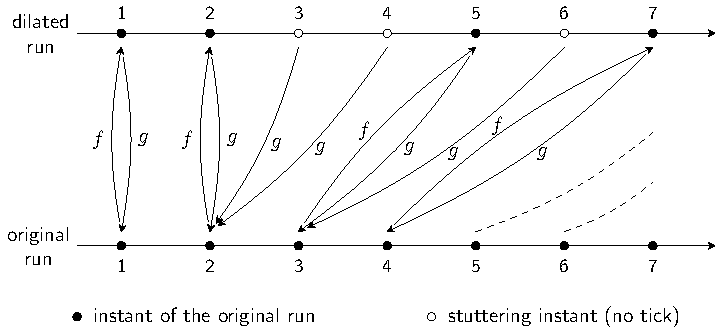
\includegraphics{dilating.pdf}
    \caption{Dilating and contracting functions}\label{fig:dilating-run}
  \end{figure}%
\end{isamarkuptext}\isamarkuptrue%
%
\begin{isamarkuptext}%
A function \isa{g} is contracting with respect to the dilation of run
\isa{sub} into run \isa{r} by the dilating function \isa{f} if:

%
\begin{itemize}%
\item it is a contracting function ;

\item \isa{{\isacharparenleft}f\ {\isasymcirc}\ g{\isacharparenright}\ n} is the index of the last original instant before instant 
\isa{n} in run \isa{r}, therefore:

%
\begin{itemize}%
\item \isa{{\isacharparenleft}f\ {\isasymcirc}\ g{\isacharparenright}\ n\ {\isasymle}\ n}

\item the time does not change on any clock between instants \isa{{\isacharparenleft}f\ {\isasymcirc}\ g{\isacharparenright}\ n}
and \isa{n} of run \isa{r};

\item no clock ticks before \isa{n} strictly after \isa{{\isacharparenleft}f\ {\isasymcirc}\ g{\isacharparenright}\ n} 
in run \isa{r}.
See \autoref{fig:dilating-run} for a better understanding. Notice that in this 
example, \isa{{\isadigit{2}}} is equal to \isa{{\isacharparenleft}f\ {\isasymcirc}\ g{\isacharparenright}\ {\isadigit{2}}}, \isa{{\isacharparenleft}f\ {\isasymcirc}\ g{\isacharparenright}\ {\isadigit{3}}}, 
and \isa{{\isacharparenleft}f\ {\isasymcirc}\ g{\isacharparenright}\ {\isadigit{4}}}. %
\end{itemize}%
\end{itemize}%
\end{isamarkuptext}\isamarkuptrue%
\isanewline
\isacommand{definition}\isamarkupfalse%
\ contracting\isanewline
\isakeyword{where}\ \isanewline
\ \ {\isacartoucheopen}contracting\ g\ r\ sub\ f\ {\isasymequiv}\ \ contracting{\isacharunderscore}fun\ g\isanewline
\ \ \ \ \ \ \ \ \ \ \ \ \ \ \ \ \ \ \ \ \ \ \ \ \ \ {\isasymand}\ {\isacharparenleft}{\isasymforall}n{\isachardot}\ f\ {\isacharparenleft}g\ n{\isacharparenright}\ {\isasymle}\ n{\isacharparenright}\isanewline
\ \ \ \ \ \ \ \ \ \ \ \ \ \ \ \ \ \ \ \ \ \ \ \ \ \ {\isasymand}\ {\isacharparenleft}{\isasymforall}n\ c\ k{\isachardot}\ f\ {\isacharparenleft}g\ n{\isacharparenright}\ {\isasymle}\ k\ {\isasymand}\ k\ {\isasymle}\ n\isanewline
\ \ \ \ \ \ \ \ \ \ \ \ \ \ \ \ \ \ \ \ \ \ \ \ \ \ \ \ \ \ {\isasymlongrightarrow}\ time\ {\isacharparenleft}{\isacharparenleft}Rep{\isacharunderscore}run\ r{\isacharparenright}\ k\ c{\isacharparenright}\ {\isacharequal}\ time\ {\isacharparenleft}{\isacharparenleft}Rep{\isacharunderscore}run\ sub{\isacharparenright}\ {\isacharparenleft}g\ n{\isacharparenright}\ c{\isacharparenright}{\isacharparenright}\isanewline
\ \ \ \ \ \ \ \ \ \ \ \ \ \ \ \ \ \ \ \ \ \ \ \ \ \ {\isasymand}\ {\isacharparenleft}{\isasymforall}n\ c\ k{\isachardot}\ f\ {\isacharparenleft}g\ n{\isacharparenright}\ {\isacharless}\ k\ {\isasymand}\ k\ {\isasymle}\ n\isanewline
\ \ \ \ \ \ \ \ \ \ \ \ \ \ \ \ \ \ \ \ \ \ \ \ \ \ \ \ \ \ {\isasymlongrightarrow}\ {\isasymnot}\ hamlet\ {\isacharparenleft}{\isacharparenleft}Rep{\isacharunderscore}run\ r{\isacharparenright}\ k\ c{\isacharparenright}{\isacharparenright}{\isacartoucheclose}%
\begin{isamarkuptext}%
For any dilating function, we can build its \emph{inverse}, as illustrated on
  \autoref{fig:dilating-run}, which is a contracting function:%
\end{isamarkuptext}\isamarkuptrue%
\isacommand{definition}\isamarkupfalse%
\ {\isacartoucheopen}dil{\isacharunderscore}inverse\ f{\isacharcolon}{\isacharcolon}{\isacharparenleft}nat\ {\isasymRightarrow}\ nat{\isacharparenright}\ {\isasymequiv}\ {\isacharparenleft}{\isasymlambda}n{\isachardot}\ Max\ {\isacharbraceleft}i{\isachardot}\ f\ i\ {\isasymle}\ n{\isacharbraceright}{\isacharparenright}{\isacartoucheclose}%
\isadelimdocument
%
\endisadelimdocument
%
\isatagdocument
%
\isamarkupsubsection{Alternate definitions for counting ticks.%
}
\isamarkuptrue%
%
\endisatagdocument
{\isafolddocument}%
%
\isadelimdocument
%
\endisadelimdocument
%
\begin{isamarkuptext}%
For proving the stuttering invariance of TESL specifications, we will need
  these alternate definitions for counting ticks, which are based on sets.%
\end{isamarkuptext}\isamarkuptrue%
%
\begin{isamarkuptext}%
\isa{tick{\isacharunderscore}count\ r\ c\ n} is the number of ticks of clock \isa{c} in 
  run \isa{r} upto instant \isa{n}.%
\end{isamarkuptext}\isamarkuptrue%
\isacommand{definition}\isamarkupfalse%
\ tick{\isacharunderscore}count\ {\isacharcolon}{\isacharcolon}\ {\isacartoucheopen}{\isacharprime}a{\isacharcolon}{\isacharcolon}linordered{\isacharunderscore}field\ run\ {\isasymRightarrow}\ clock\ {\isasymRightarrow}\ nat\ {\isasymRightarrow}\ nat{\isacartoucheclose}\isanewline
\isakeyword{where}\isanewline
\ \ {\isacartoucheopen}tick{\isacharunderscore}count\ r\ c\ n\ {\isacharequal}\ card\ {\isacharbraceleft}i{\isachardot}\ i\ {\isasymle}\ n\ {\isasymand}\ hamlet\ {\isacharparenleft}{\isacharparenleft}Rep{\isacharunderscore}run\ r{\isacharparenright}\ i\ c{\isacharparenright}{\isacharbraceright}{\isacartoucheclose}%
\begin{isamarkuptext}%
\isa{tick{\isacharunderscore}count{\isacharunderscore}strict\ r\ c\ n} is the number of ticks of clock \isa{c} 
  in run \isa{r} upto but excluding instant \isa{n}.%
\end{isamarkuptext}\isamarkuptrue%
\isacommand{definition}\isamarkupfalse%
\ tick{\isacharunderscore}count{\isacharunderscore}strict\ {\isacharcolon}{\isacharcolon}\ {\isacartoucheopen}{\isacharprime}a{\isacharcolon}{\isacharcolon}linordered{\isacharunderscore}field\ run\ {\isasymRightarrow}\ clock\ {\isasymRightarrow}\ nat\ {\isasymRightarrow}\ nat{\isacartoucheclose}\isanewline
\isakeyword{where}\isanewline
\ \ {\isacartoucheopen}tick{\isacharunderscore}count{\isacharunderscore}strict\ r\ c\ n\ {\isacharequal}\ card\ {\isacharbraceleft}i{\isachardot}\ i\ {\isacharless}\ n\ {\isasymand}\ hamlet\ {\isacharparenleft}{\isacharparenleft}Rep{\isacharunderscore}run\ r{\isacharparenright}\ i\ c{\isacharparenright}{\isacharbraceright}{\isacartoucheclose}\isanewline
\isanewline
%
\isadelimtheory
\isanewline
%
\endisadelimtheory
%
\isatagtheory
\isacommand{end}\isamarkupfalse%
%
\endisatagtheory
{\isafoldtheory}%
%
\isadelimtheory
%
\endisadelimtheory
%
\end{isabellebody}%
\endinput
%:%file=~/Documents/Recherche/Thesards/2014_Hai_NGUYEN_VAN/Heron_git/reiher2/reiher/src/StutteringDefs.thy%:%
%:%11=1%:%
%:%15=3%:%
%:%31=5%:%
%:%32=5%:%
%:%33=6%:%
%:%34=7%:%
%:%35=8%:%
%:%36=9%:%
%:%45=12%:%
%:%46=13%:%
%:%47=14%:%
%:%48=15%:%
%:%49=16%:%
%:%58=19%:%
%:%70=22%:%
%:%71=23%:%
%:%72=24%:%
%:%73=25%:%
%:%74=26%:%
%:%78=27%:%
%:%80=28%:%
%:%81=29%:%
%:%83=30%:%
%:%84=31%:%
%:%86=32%:%
%:%87=33%:%
%:%90=35%:%
%:%91=35%:%
%:%92=36%:%
%:%93=37%:%
%:%100=45%:%
%:%101=46%:%
%:%105=47%:%
%:%107=48%:%
%:%109=49%:%
%:%112=51%:%
%:%113=51%:%
%:%114=52%:%
%:%115=53%:%
%:%119=58%:%
%:%121=60%:%
%:%122=60%:%
%:%123=61%:%
%:%124=62%:%
%:%126=65%:%
%:%127=66%:%
%:%128=67%:%
%:%129=68%:%
%:%130=69%:%
%:%131=70%:%
%:%132=71%:%
%:%134=73%:%
%:%135=73%:%
%:%136=74%:%
%:%138=77%:%
%:%139=78%:%
%:%140=79%:%
%:%141=80%:%
%:%142=81%:%
%:%143=82%:%
%:%144=83%:%
%:%145=84%:%
%:%149=96%:%
%:%150=97%:%
%:%154=98%:%
%:%156=99%:%
%:%157=100%:%
%:%163=102%:%
%:%164=103%:%
%:%166=104%:%
%:%167=105%:%
%:%168=106%:%
%:%169=107%:%
%:%170=108%:%
%:%174=115%:%
%:%175=116%:%
%:%176=116%:%
%:%177=117%:%
%:%178=118%:%
%:%185=126%:%
%:%186=127%:%
%:%188=129%:%
%:%189=129%:%
%:%196=132%:%
%:%208=135%:%
%:%209=136%:%
%:%213=140%:%
%:%214=141%:%
%:%216=143%:%
%:%217=143%:%
%:%218=144%:%
%:%219=145%:%
%:%221=148%:%
%:%222=149%:%
%:%224=151%:%
%:%225=151%:%
%:%226=152%:%
%:%227=153%:%
%:%228=154%:%
%:%231=155%:%
%:%236=156%:%

%
\begin{isabellebody}%
\setisabellecontext{StutteringLemmas}%
%
\isadelimdocument
%
\endisadelimdocument
%
\isatagdocument
%
\isamarkupsubsection{Stuttering Lemmas%
}
\isamarkuptrue%
%
\endisatagdocument
{\isafolddocument}%
%
\isadelimdocument
%
\endisadelimdocument
%
\isadelimtheory
%
\endisadelimtheory
%
\isatagtheory
\isacommand{theory}\isamarkupfalse%
\ StutteringLemmas\isanewline
\isanewline
\isakeyword{imports}\ StutteringDefs\isanewline
\isanewline
\isakeyword{begin}%
\endisatagtheory
{\isafoldtheory}%
%
\isadelimtheory
%
\endisadelimtheory
%
\begin{isamarkuptext}%
In this section, we prove several lemmas that will be used to show that TESL 
  specifications are invariant by stuttering.

  The following one will be useful in proving properties over a sequence of 
  stuttering instants.%
\end{isamarkuptext}\isamarkuptrue%
\isacommand{lemma}\isamarkupfalse%
\ bounded{\isacharunderscore}suc{\isacharunderscore}ind{\isacharcolon}\isanewline
\ \ \isakeyword{assumes}\ {\isacartoucheopen}{\isasymAnd}k{\isachardot}\ k\ {\isacharless}\ m\ {\isasymLongrightarrow}\ P\ {\isacharparenleft}Suc\ {\isacharparenleft}z\ {\isacharplus}\ k{\isacharparenright}{\isacharparenright}\ {\isacharequal}\ P\ {\isacharparenleft}z\ {\isacharplus}\ k{\isacharparenright}{\isacartoucheclose}\isanewline
\ \ \ \ \isakeyword{shows}\ {\isacartoucheopen}k\ {\isacharless}\ m\ {\isasymLongrightarrow}\ P\ {\isacharparenleft}Suc\ {\isacharparenleft}z\ {\isacharplus}\ k{\isacharparenright}{\isacharparenright}\ {\isacharequal}\ P\ z{\isacartoucheclose}\isanewline
%
\isadelimproof
%
\endisadelimproof
%
\isatagproof
\isacommand{proof}\isamarkupfalse%
\ {\isacharparenleft}induction\ k{\isacharparenright}\isanewline
\ \ \isacommand{case}\isamarkupfalse%
\ {\isadigit{0}}\isanewline
\ \ \ \ \isacommand{with}\isamarkupfalse%
\ assms{\isacharparenleft}{\isadigit{1}}{\isacharparenright}{\isacharbrackleft}of\ {\isadigit{0}}{\isacharbrackright}\ \isacommand{show}\isamarkupfalse%
\ {\isacharquery}case\ \isacommand{by}\isamarkupfalse%
\ simp\isanewline
\isacommand{next}\isamarkupfalse%
\isanewline
\ \ \isacommand{case}\isamarkupfalse%
\ {\isacharparenleft}Suc\ k{\isacharprime}{\isacharparenright}\isanewline
\ \ \ \ \isacommand{with}\isamarkupfalse%
\ assms{\isacharbrackleft}of\ {\isacartoucheopen}Suc\ k{\isacharprime}{\isacartoucheclose}{\isacharbrackright}\ \isacommand{show}\isamarkupfalse%
\ {\isacharquery}case\ \isacommand{by}\isamarkupfalse%
\ force\isanewline
\isacommand{qed}\isamarkupfalse%
%
\endisatagproof
{\isafoldproof}%
%
\isadelimproof
%
\endisadelimproof
%
\isadelimdocument
%
\endisadelimdocument
%
\isatagdocument
%
\isamarkupsubsection{Lemmas used to prove the invariance by stuttering%
}
\isamarkuptrue%
%
\endisatagdocument
{\isafolddocument}%
%
\isadelimdocument
%
\endisadelimdocument
%
\begin{isamarkuptext}%
Since a dilating function is strictly monotonous, it is injective.%
\end{isamarkuptext}\isamarkuptrue%
\isacommand{lemma}\isamarkupfalse%
\ dilating{\isacharunderscore}fun{\isacharunderscore}injects{\isacharcolon}\isanewline
\ \ \isakeyword{assumes}\ {\isacartoucheopen}dilating{\isacharunderscore}fun\ f\ r{\isacartoucheclose}\isanewline
\ \ \isakeyword{shows}\ \ \ {\isacartoucheopen}inj{\isacharunderscore}on\ f\ A{\isacartoucheclose}\isanewline
%
\isadelimproof
%
\endisadelimproof
%
\isatagproof
\isacommand{using}\isamarkupfalse%
\ assms\ dilating{\isacharunderscore}fun{\isacharunderscore}def\ strict{\isacharunderscore}mono{\isacharunderscore}imp{\isacharunderscore}inj{\isacharunderscore}on\ \isacommand{by}\isamarkupfalse%
\ blast%
\endisatagproof
{\isafoldproof}%
%
\isadelimproof
\isanewline
%
\endisadelimproof
\isanewline
\isacommand{lemma}\isamarkupfalse%
\ dilating{\isacharunderscore}injects{\isacharcolon}\isanewline
\ \ \isakeyword{assumes}\ {\isacartoucheopen}dilating\ f\ sub\ r{\isacartoucheclose}\isanewline
\ \ \isakeyword{shows}\ \ \ {\isacartoucheopen}inj{\isacharunderscore}on\ f\ A{\isacartoucheclose}\isanewline
%
\isadelimproof
%
\endisadelimproof
%
\isatagproof
\isacommand{using}\isamarkupfalse%
\ assms\ dilating{\isacharunderscore}def\ dilating{\isacharunderscore}fun{\isacharunderscore}injects\ \isacommand{by}\isamarkupfalse%
\ blast%
\endisatagproof
{\isafoldproof}%
%
\isadelimproof
%
\endisadelimproof
%
\begin{isamarkuptext}%
If a clock ticks at an instant in a dilated run, that instant is the image
  by the dilating function of an instant of the original run.%
\end{isamarkuptext}\isamarkuptrue%
\isacommand{lemma}\isamarkupfalse%
\ ticks{\isacharunderscore}image{\isacharcolon}\isanewline
\ \ \isakeyword{assumes}\ {\isacartoucheopen}dilating{\isacharunderscore}fun\ f\ r{\isacartoucheclose}\isanewline
\ \ \isakeyword{and}\ \ \ \ \ {\isacartoucheopen}hamlet\ {\isacharparenleft}{\isacharparenleft}Rep{\isacharunderscore}run\ r{\isacharparenright}\ n\ c{\isacharparenright}{\isacartoucheclose}\isanewline
\ \ \isakeyword{shows}\ \ \ {\isacartoucheopen}{\isasymexists}n\isactrlsub {\isadigit{0}}{\isachardot}\ f\ n\isactrlsub {\isadigit{0}}\ {\isacharequal}\ n{\isacartoucheclose}\isanewline
%
\isadelimproof
%
\endisadelimproof
%
\isatagproof
\isacommand{using}\isamarkupfalse%
\ dilating{\isacharunderscore}fun{\isacharunderscore}def\ assms\ \isacommand{by}\isamarkupfalse%
\ blast%
\endisatagproof
{\isafoldproof}%
%
\isadelimproof
\isanewline
%
\endisadelimproof
\isanewline
\isacommand{lemma}\isamarkupfalse%
\ ticks{\isacharunderscore}image{\isacharunderscore}sub{\isacharcolon}\isanewline
\ \ \isakeyword{assumes}\ {\isacartoucheopen}dilating\ f\ sub\ r{\isacartoucheclose}\isanewline
\ \ \isakeyword{and}\ \ \ \ \ {\isacartoucheopen}hamlet\ {\isacharparenleft}{\isacharparenleft}Rep{\isacharunderscore}run\ r{\isacharparenright}\ n\ c{\isacharparenright}{\isacartoucheclose}\isanewline
\ \ \isakeyword{shows}\ \ \ {\isacartoucheopen}{\isasymexists}n\isactrlsub {\isadigit{0}}{\isachardot}\ f\ n\isactrlsub {\isadigit{0}}\ {\isacharequal}\ n{\isacartoucheclose}\isanewline
%
\isadelimproof
%
\endisadelimproof
%
\isatagproof
\isacommand{using}\isamarkupfalse%
\ assms\ dilating{\isacharunderscore}def\ ticks{\isacharunderscore}image\ \isacommand{by}\isamarkupfalse%
\ blast%
\endisatagproof
{\isafoldproof}%
%
\isadelimproof
\isanewline
%
\endisadelimproof
\isanewline
\isacommand{lemma}\isamarkupfalse%
\ ticks{\isacharunderscore}image{\isacharunderscore}sub{\isacharprime}{\isacharcolon}\isanewline
\ \ \isakeyword{assumes}\ {\isacartoucheopen}dilating\ f\ sub\ r{\isacartoucheclose}\isanewline
\ \ \isakeyword{and}\ \ \ \ \ {\isacartoucheopen}{\isasymexists}c{\isachardot}\ hamlet\ {\isacharparenleft}{\isacharparenleft}Rep{\isacharunderscore}run\ r{\isacharparenright}\ n\ c{\isacharparenright}{\isacartoucheclose}\isanewline
\ \ \isakeyword{shows}\ \ \ {\isacartoucheopen}{\isasymexists}n\isactrlsub {\isadigit{0}}{\isachardot}\ f\ n\isactrlsub {\isadigit{0}}\ {\isacharequal}\ n{\isacartoucheclose}\isanewline
%
\isadelimproof
%
\endisadelimproof
%
\isatagproof
\isacommand{using}\isamarkupfalse%
\ ticks{\isacharunderscore}image{\isacharunderscore}sub{\isacharbrackleft}OF\ assms{\isacharparenleft}{\isadigit{1}}{\isacharparenright}{\isacharbrackright}\ assms{\isacharparenleft}{\isadigit{2}}{\isacharparenright}\ \isacommand{by}\isamarkupfalse%
\ blast%
\endisatagproof
{\isafoldproof}%
%
\isadelimproof
%
\endisadelimproof
%
\begin{isamarkuptext}%
The image of the ticks in an interval by a dilating function is the interval 
  bounded by the image of the bounds of the original interval.
  This is proven for all 4 kinds of intervals:  \isatt{]m{\char`\,}\ n[}, \isatt{[m{\char`\,}\ n[}, \isatt{]m{\char`\,}\ n]}
  and \isatt{[m{\char`\,}\ n]}.%
\end{isamarkuptext}\isamarkuptrue%
\isacommand{lemma}\isamarkupfalse%
\ dilating{\isacharunderscore}fun{\isacharunderscore}image{\isacharunderscore}strict{\isacharcolon}\isanewline
\ \ \isakeyword{assumes}\ {\isacartoucheopen}dilating{\isacharunderscore}fun\ f\ r{\isacartoucheclose}\isanewline
\ \ \isakeyword{shows}\ \ \ {\isacartoucheopen}{\isacharbraceleft}k{\isachardot}\ f\ m\ {\isacharless}\ k\ {\isasymand}\ k\ {\isacharless}\ f\ n\ {\isasymand}\ hamlet\ {\isacharparenleft}{\isacharparenleft}Rep{\isacharunderscore}run\ r{\isacharparenright}\ k\ c{\isacharparenright}{\isacharbraceright}\isanewline
\ \ \ \ \ \ \ \ \ \ \ \ {\isacharequal}\ image\ f\ {\isacharbraceleft}k{\isachardot}\ m\ {\isacharless}\ k\ {\isasymand}\ k\ {\isacharless}\ n\ {\isasymand}\ hamlet\ {\isacharparenleft}{\isacharparenleft}Rep{\isacharunderscore}run\ r{\isacharparenright}\ {\isacharparenleft}f\ k{\isacharparenright}\ c{\isacharparenright}{\isacharbraceright}{\isacartoucheclose}\isanewline
\ \ {\isacharparenleft}\isakeyword{is}\ {\isacartoucheopen}{\isacharquery}IMG\ {\isacharequal}\ image\ f\ {\isacharquery}SET{\isacartoucheclose}{\isacharparenright}\isanewline
%
\isadelimproof
%
\endisadelimproof
%
\isatagproof
\isacommand{proof}\isamarkupfalse%
\isanewline
\ \ \isacommand{{\isacharbraceleft}}\isamarkupfalse%
\ \isacommand{fix}\isamarkupfalse%
\ k\ \isacommand{assume}\isamarkupfalse%
\ h{\isacharcolon}{\isacartoucheopen}k\ {\isasymin}\ {\isacharquery}IMG{\isacartoucheclose}\isanewline
\ \ \ \ \isacommand{from}\isamarkupfalse%
\ h\ \isacommand{obtain}\isamarkupfalse%
\ k\isactrlsub {\isadigit{0}}\ \isakeyword{where}\ k{\isadigit{0}}prop{\isacharcolon}{\isacartoucheopen}f\ k\isactrlsub {\isadigit{0}}\ {\isacharequal}\ k\ {\isasymand}\ hamlet\ {\isacharparenleft}{\isacharparenleft}Rep{\isacharunderscore}run\ r{\isacharparenright}\ {\isacharparenleft}f\ k\isactrlsub {\isadigit{0}}{\isacharparenright}\ c{\isacharparenright}{\isacartoucheclose}\isanewline
\ \ \ \ \ \ \isacommand{using}\isamarkupfalse%
\ ticks{\isacharunderscore}image{\isacharbrackleft}OF\ assms{\isacharbrackright}\ \isacommand{by}\isamarkupfalse%
\ blast\isanewline
\ \ \ \ \isacommand{with}\isamarkupfalse%
\ h\ \isacommand{have}\isamarkupfalse%
\ {\isacartoucheopen}k\ {\isasymin}\ image\ f\ {\isacharquery}SET{\isacartoucheclose}\isanewline
\ \ \ \ \ \ \isacommand{using}\isamarkupfalse%
\ assms\ dilating{\isacharunderscore}fun{\isacharunderscore}def\ strict{\isacharunderscore}mono{\isacharunderscore}less\ \isacommand{by}\isamarkupfalse%
\ blast\isanewline
\ \ \isacommand{{\isacharbraceright}}\isamarkupfalse%
\ \isacommand{thus}\isamarkupfalse%
\ {\isacartoucheopen}{\isacharquery}IMG\ {\isasymsubseteq}\ image\ f\ {\isacharquery}SET{\isacartoucheclose}\ \isacommand{{\isachardot}{\isachardot}}\isamarkupfalse%
\isanewline
\isacommand{next}\isamarkupfalse%
\isanewline
\ \ \isacommand{{\isacharbraceleft}}\isamarkupfalse%
\ \isacommand{fix}\isamarkupfalse%
\ k\ \isacommand{assume}\isamarkupfalse%
\ h{\isacharcolon}{\isacartoucheopen}k\ {\isasymin}\ image\ f\ {\isacharquery}SET{\isacartoucheclose}\isanewline
\ \ \ \ \isacommand{from}\isamarkupfalse%
\ h\ \isacommand{obtain}\isamarkupfalse%
\ k\isactrlsub {\isadigit{0}}\ \isakeyword{where}\ k{\isadigit{0}}prop{\isacharcolon}{\isacartoucheopen}k\ {\isacharequal}\ f\ k\isactrlsub {\isadigit{0}}\ {\isasymand}\ k\isactrlsub {\isadigit{0}}\ {\isasymin}\ {\isacharquery}SET{\isacartoucheclose}\ \isacommand{by}\isamarkupfalse%
\ blast\isanewline
\ \ \ \ \isacommand{hence}\isamarkupfalse%
\ {\isacartoucheopen}k\ {\isasymin}\ {\isacharquery}IMG{\isacartoucheclose}\ \isacommand{using}\isamarkupfalse%
\ assms\ \isacommand{by}\isamarkupfalse%
\ {\isacharparenleft}simp\ add{\isacharcolon}\ dilating{\isacharunderscore}fun{\isacharunderscore}def\ strict{\isacharunderscore}mono{\isacharunderscore}less{\isacharparenright}\isanewline
\ \ \isacommand{{\isacharbraceright}}\isamarkupfalse%
\ \isacommand{thus}\isamarkupfalse%
\ {\isacartoucheopen}image\ f\ {\isacharquery}SET\ {\isasymsubseteq}\ {\isacharquery}IMG{\isacartoucheclose}\ \isacommand{{\isachardot}{\isachardot}}\isamarkupfalse%
\isanewline
\isacommand{qed}\isamarkupfalse%
%
\endisatagproof
{\isafoldproof}%
%
\isadelimproof
\isanewline
%
\endisadelimproof
\isanewline
\isacommand{lemma}\isamarkupfalse%
\ dilating{\isacharunderscore}fun{\isacharunderscore}image{\isacharunderscore}left{\isacharcolon}\isanewline
\ \ \isakeyword{assumes}\ {\isacartoucheopen}dilating{\isacharunderscore}fun\ f\ r{\isacartoucheclose}\isanewline
\ \ \isakeyword{shows}\ \ \ {\isacartoucheopen}{\isacharbraceleft}k{\isachardot}\ f\ m\ {\isasymle}\ k\ {\isasymand}\ k\ {\isacharless}\ f\ n\ {\isasymand}\ hamlet\ {\isacharparenleft}{\isacharparenleft}Rep{\isacharunderscore}run\ r{\isacharparenright}\ k\ c{\isacharparenright}{\isacharbraceright}\isanewline
\ \ \ \ \ \ \ \ \ \ {\isacharequal}\ image\ f\ {\isacharbraceleft}k{\isachardot}\ m\ {\isasymle}\ k\ {\isasymand}\ k\ {\isacharless}\ n\ {\isasymand}\ hamlet\ {\isacharparenleft}{\isacharparenleft}Rep{\isacharunderscore}run\ r{\isacharparenright}\ {\isacharparenleft}f\ k{\isacharparenright}\ c{\isacharparenright}{\isacharbraceright}{\isacartoucheclose}\isanewline
\ \ {\isacharparenleft}\isakeyword{is}\ {\isacartoucheopen}{\isacharquery}IMG\ {\isacharequal}\ image\ f\ {\isacharquery}SET{\isacartoucheclose}{\isacharparenright}\isanewline
%
\isadelimproof
%
\endisadelimproof
%
\isatagproof
\isacommand{proof}\isamarkupfalse%
\isanewline
\ \ \isacommand{{\isacharbraceleft}}\isamarkupfalse%
\ \isacommand{fix}\isamarkupfalse%
\ k\ \isacommand{assume}\isamarkupfalse%
\ h{\isacharcolon}{\isacartoucheopen}k\ {\isasymin}\ {\isacharquery}IMG{\isacartoucheclose}\isanewline
\ \ \ \ \isacommand{from}\isamarkupfalse%
\ h\ \isacommand{obtain}\isamarkupfalse%
\ k\isactrlsub {\isadigit{0}}\ \isakeyword{where}\ k{\isadigit{0}}prop{\isacharcolon}{\isacartoucheopen}f\ k\isactrlsub {\isadigit{0}}\ {\isacharequal}\ k\ {\isasymand}\ hamlet\ {\isacharparenleft}{\isacharparenleft}Rep{\isacharunderscore}run\ r{\isacharparenright}\ {\isacharparenleft}f\ k\isactrlsub {\isadigit{0}}{\isacharparenright}\ c{\isacharparenright}{\isacartoucheclose}\isanewline
\ \ \ \ \ \ \isacommand{using}\isamarkupfalse%
\ ticks{\isacharunderscore}image{\isacharbrackleft}OF\ assms{\isacharbrackright}\ \isacommand{by}\isamarkupfalse%
\ blast\isanewline
\ \ \ \ \isacommand{with}\isamarkupfalse%
\ h\ \isacommand{have}\isamarkupfalse%
\ {\isacartoucheopen}k\ {\isasymin}\ image\ f\ {\isacharquery}SET{\isacartoucheclose}\isanewline
\ \ \ \ \ \ \isacommand{using}\isamarkupfalse%
\ assms\ dilating{\isacharunderscore}fun{\isacharunderscore}def\ strict{\isacharunderscore}mono{\isacharunderscore}less\ strict{\isacharunderscore}mono{\isacharunderscore}less{\isacharunderscore}eq\ \isacommand{by}\isamarkupfalse%
\ fastforce\isanewline
\ \ \isacommand{{\isacharbraceright}}\isamarkupfalse%
\ \isacommand{thus}\isamarkupfalse%
\ {\isacartoucheopen}{\isacharquery}IMG\ {\isasymsubseteq}\ image\ f\ {\isacharquery}SET{\isacartoucheclose}\ \isacommand{{\isachardot}{\isachardot}}\isamarkupfalse%
\isanewline
\isacommand{next}\isamarkupfalse%
\isanewline
\ \ \isacommand{{\isacharbraceleft}}\isamarkupfalse%
\ \isacommand{fix}\isamarkupfalse%
\ k\ \isacommand{assume}\isamarkupfalse%
\ h{\isacharcolon}{\isacartoucheopen}k\ {\isasymin}\ image\ f\ {\isacharquery}SET{\isacartoucheclose}\isanewline
\ \ \ \ \isacommand{from}\isamarkupfalse%
\ h\ \isacommand{obtain}\isamarkupfalse%
\ k\isactrlsub {\isadigit{0}}\ \isakeyword{where}\ k{\isadigit{0}}prop{\isacharcolon}{\isacartoucheopen}k\ {\isacharequal}\ f\ k\isactrlsub {\isadigit{0}}\ {\isasymand}\ k\isactrlsub {\isadigit{0}}\ {\isasymin}\ {\isacharquery}SET{\isacartoucheclose}\ \isacommand{by}\isamarkupfalse%
\ blast\isanewline
\ \ \ \ \isacommand{hence}\isamarkupfalse%
\ {\isacartoucheopen}k\ {\isasymin}\ {\isacharquery}IMG{\isacartoucheclose}\isanewline
\ \ \ \ \ \ \isacommand{using}\isamarkupfalse%
\ assms\ dilating{\isacharunderscore}fun{\isacharunderscore}def\ strict{\isacharunderscore}mono{\isacharunderscore}less\ strict{\isacharunderscore}mono{\isacharunderscore}less{\isacharunderscore}eq\ \isacommand{by}\isamarkupfalse%
\ fastforce\isanewline
\ \ \isacommand{{\isacharbraceright}}\isamarkupfalse%
\ \isacommand{thus}\isamarkupfalse%
\ {\isacartoucheopen}image\ f\ {\isacharquery}SET\ {\isasymsubseteq}\ {\isacharquery}IMG{\isacartoucheclose}\ \isacommand{{\isachardot}{\isachardot}}\isamarkupfalse%
\isanewline
\isacommand{qed}\isamarkupfalse%
%
\endisatagproof
{\isafoldproof}%
%
\isadelimproof
\isanewline
%
\endisadelimproof
\isanewline
\isacommand{lemma}\isamarkupfalse%
\ dilating{\isacharunderscore}fun{\isacharunderscore}image{\isacharunderscore}right{\isacharcolon}\isanewline
\ \ \isakeyword{assumes}\ {\isacartoucheopen}dilating{\isacharunderscore}fun\ f\ r{\isacartoucheclose}\isanewline
\ \ \isakeyword{shows}\ \ \ {\isacartoucheopen}{\isacharbraceleft}k{\isachardot}\ f\ m\ {\isacharless}\ k\ {\isasymand}\ k\ {\isasymle}\ f\ n\ {\isasymand}\ hamlet\ {\isacharparenleft}{\isacharparenleft}Rep{\isacharunderscore}run\ r{\isacharparenright}\ k\ c{\isacharparenright}{\isacharbraceright}\isanewline
\ \ \ \ \ \ \ \ \ \ {\isacharequal}\ image\ f\ {\isacharbraceleft}k{\isachardot}\ m\ {\isacharless}\ k\ {\isasymand}\ k\ {\isasymle}\ n\ {\isasymand}\ hamlet\ {\isacharparenleft}{\isacharparenleft}Rep{\isacharunderscore}run\ r{\isacharparenright}\ {\isacharparenleft}f\ k{\isacharparenright}\ c{\isacharparenright}{\isacharbraceright}{\isacartoucheclose}\isanewline
\ \ {\isacharparenleft}\isakeyword{is}\ {\isacartoucheopen}{\isacharquery}IMG\ {\isacharequal}\ image\ f\ {\isacharquery}SET{\isacartoucheclose}{\isacharparenright}\isanewline
%
\isadelimproof
%
\endisadelimproof
%
\isatagproof
\isacommand{proof}\isamarkupfalse%
\isanewline
\ \ \isacommand{{\isacharbraceleft}}\isamarkupfalse%
\ \isacommand{fix}\isamarkupfalse%
\ k\ \isacommand{assume}\isamarkupfalse%
\ h{\isacharcolon}{\isacartoucheopen}k\ {\isasymin}\ {\isacharquery}IMG{\isacartoucheclose}\isanewline
\ \ \ \ \isacommand{from}\isamarkupfalse%
\ h\ \isacommand{obtain}\isamarkupfalse%
\ k\isactrlsub {\isadigit{0}}\ \isakeyword{where}\ k{\isadigit{0}}prop{\isacharcolon}{\isacartoucheopen}f\ k\isactrlsub {\isadigit{0}}\ {\isacharequal}\ k\ {\isasymand}\ hamlet\ {\isacharparenleft}{\isacharparenleft}Rep{\isacharunderscore}run\ r{\isacharparenright}\ {\isacharparenleft}f\ k\isactrlsub {\isadigit{0}}{\isacharparenright}\ c{\isacharparenright}{\isacartoucheclose}\isanewline
\ \ \ \ \ \ \isacommand{using}\isamarkupfalse%
\ ticks{\isacharunderscore}image{\isacharbrackleft}OF\ assms{\isacharbrackright}\ \isacommand{by}\isamarkupfalse%
\ blast\isanewline
\ \ \ \ \isacommand{with}\isamarkupfalse%
\ h\ \isacommand{have}\isamarkupfalse%
\ {\isacartoucheopen}k\ {\isasymin}\ image\ f\ {\isacharquery}SET{\isacartoucheclose}\isanewline
\ \ \ \ \ \ \isacommand{using}\isamarkupfalse%
\ assms\ dilating{\isacharunderscore}fun{\isacharunderscore}def\ strict{\isacharunderscore}mono{\isacharunderscore}less\ strict{\isacharunderscore}mono{\isacharunderscore}less{\isacharunderscore}eq\ \isacommand{by}\isamarkupfalse%
\ fastforce\isanewline
\ \ \isacommand{{\isacharbraceright}}\isamarkupfalse%
\ \isacommand{thus}\isamarkupfalse%
\ {\isacartoucheopen}{\isacharquery}IMG\ {\isasymsubseteq}\ image\ f\ {\isacharquery}SET{\isacartoucheclose}\ \isacommand{{\isachardot}{\isachardot}}\isamarkupfalse%
\isanewline
\isacommand{next}\isamarkupfalse%
\isanewline
\ \ \isacommand{{\isacharbraceleft}}\isamarkupfalse%
\ \isacommand{fix}\isamarkupfalse%
\ k\ \isacommand{assume}\isamarkupfalse%
\ h{\isacharcolon}{\isacartoucheopen}k\ {\isasymin}\ image\ f\ {\isacharquery}SET{\isacartoucheclose}\isanewline
\ \ \ \ \isacommand{from}\isamarkupfalse%
\ h\ \isacommand{obtain}\isamarkupfalse%
\ k\isactrlsub {\isadigit{0}}\ \isakeyword{where}\ k{\isadigit{0}}prop{\isacharcolon}{\isacartoucheopen}k\ {\isacharequal}\ f\ k\isactrlsub {\isadigit{0}}\ {\isasymand}\ k\isactrlsub {\isadigit{0}}\ {\isasymin}\ {\isacharquery}SET{\isacartoucheclose}\ \isacommand{by}\isamarkupfalse%
\ blast\isanewline
\ \ \ \ \isacommand{hence}\isamarkupfalse%
\ {\isacartoucheopen}k\ {\isasymin}\ {\isacharquery}IMG{\isacartoucheclose}\isanewline
\ \ \ \ \ \ \isacommand{using}\isamarkupfalse%
\ assms\ dilating{\isacharunderscore}fun{\isacharunderscore}def\ strict{\isacharunderscore}mono{\isacharunderscore}less\ strict{\isacharunderscore}mono{\isacharunderscore}less{\isacharunderscore}eq\ \isacommand{by}\isamarkupfalse%
\ fastforce\isanewline
\ \ \isacommand{{\isacharbraceright}}\isamarkupfalse%
\ \isacommand{thus}\isamarkupfalse%
\ {\isacartoucheopen}image\ f\ {\isacharquery}SET\ {\isasymsubseteq}\ {\isacharquery}IMG{\isacartoucheclose}\ \isacommand{{\isachardot}{\isachardot}}\isamarkupfalse%
\isanewline
\isacommand{qed}\isamarkupfalse%
%
\endisatagproof
{\isafoldproof}%
%
\isadelimproof
\isanewline
%
\endisadelimproof
\isanewline
\isacommand{lemma}\isamarkupfalse%
\ dilating{\isacharunderscore}fun{\isacharunderscore}image{\isacharcolon}\isanewline
\ \ \isakeyword{assumes}\ {\isacartoucheopen}dilating{\isacharunderscore}fun\ f\ r{\isacartoucheclose}\isanewline
\ \ \isakeyword{shows}\ \ \ {\isacartoucheopen}{\isacharbraceleft}k{\isachardot}\ f\ m\ {\isasymle}\ k\ {\isasymand}\ k\ {\isasymle}\ f\ n\ {\isasymand}\ hamlet\ {\isacharparenleft}{\isacharparenleft}Rep{\isacharunderscore}run\ r{\isacharparenright}\ k\ c{\isacharparenright}{\isacharbraceright}\isanewline
\ \ \ \ \ \ \ \ \ \ {\isacharequal}\ image\ f\ {\isacharbraceleft}k{\isachardot}\ m\ {\isasymle}\ k\ {\isasymand}\ k\ {\isasymle}\ n\ {\isasymand}\ hamlet\ {\isacharparenleft}{\isacharparenleft}Rep{\isacharunderscore}run\ r{\isacharparenright}\ {\isacharparenleft}f\ k{\isacharparenright}\ c{\isacharparenright}{\isacharbraceright}{\isacartoucheclose}\isanewline
\ \ {\isacharparenleft}\isakeyword{is}\ {\isacartoucheopen}{\isacharquery}IMG\ {\isacharequal}\ image\ f\ {\isacharquery}SET{\isacartoucheclose}{\isacharparenright}\isanewline
%
\isadelimproof
%
\endisadelimproof
%
\isatagproof
\isacommand{proof}\isamarkupfalse%
\isanewline
\ \ \isacommand{{\isacharbraceleft}}\isamarkupfalse%
\ \isacommand{fix}\isamarkupfalse%
\ k\ \isacommand{assume}\isamarkupfalse%
\ h{\isacharcolon}{\isacartoucheopen}k\ {\isasymin}\ {\isacharquery}IMG{\isacartoucheclose}\isanewline
\ \ \ \ \isacommand{from}\isamarkupfalse%
\ h\ \isacommand{obtain}\isamarkupfalse%
\ k\isactrlsub {\isadigit{0}}\ \isakeyword{where}\ k{\isadigit{0}}prop{\isacharcolon}{\isacartoucheopen}f\ k\isactrlsub {\isadigit{0}}\ {\isacharequal}\ k\ {\isasymand}\ hamlet\ {\isacharparenleft}{\isacharparenleft}Rep{\isacharunderscore}run\ r{\isacharparenright}\ {\isacharparenleft}f\ k\isactrlsub {\isadigit{0}}{\isacharparenright}\ c{\isacharparenright}{\isacartoucheclose}\isanewline
\ \ \ \ \ \ \isacommand{using}\isamarkupfalse%
\ ticks{\isacharunderscore}image{\isacharbrackleft}OF\ assms{\isacharbrackright}\ \isacommand{by}\isamarkupfalse%
\ blast\isanewline
\ \ \ \ \isacommand{with}\isamarkupfalse%
\ h\ \isacommand{have}\isamarkupfalse%
\ {\isacartoucheopen}k\ {\isasymin}\ image\ f\ {\isacharquery}SET{\isacartoucheclose}\isanewline
\ \ \ \ \ \ \isacommand{using}\isamarkupfalse%
\ assms\ dilating{\isacharunderscore}fun{\isacharunderscore}def\ strict{\isacharunderscore}mono{\isacharunderscore}less{\isacharunderscore}eq\ \isacommand{by}\isamarkupfalse%
\ blast\isanewline
\ \ \isacommand{{\isacharbraceright}}\isamarkupfalse%
\ \isacommand{thus}\isamarkupfalse%
\ {\isacartoucheopen}{\isacharquery}IMG\ {\isasymsubseteq}\ image\ f\ {\isacharquery}SET{\isacartoucheclose}\ \isacommand{{\isachardot}{\isachardot}}\isamarkupfalse%
\isanewline
\isacommand{next}\isamarkupfalse%
\isanewline
\ \ \isacommand{{\isacharbraceleft}}\isamarkupfalse%
\ \isacommand{fix}\isamarkupfalse%
\ k\ \isacommand{assume}\isamarkupfalse%
\ h{\isacharcolon}{\isacartoucheopen}k\ {\isasymin}\ image\ f\ {\isacharquery}SET{\isacartoucheclose}\isanewline
\ \ \ \ \isacommand{from}\isamarkupfalse%
\ h\ \isacommand{obtain}\isamarkupfalse%
\ k\isactrlsub {\isadigit{0}}\ \isakeyword{where}\ k{\isadigit{0}}prop{\isacharcolon}{\isacartoucheopen}k\ {\isacharequal}\ f\ k\isactrlsub {\isadigit{0}}\ {\isasymand}\ k\isactrlsub {\isadigit{0}}\ {\isasymin}\ {\isacharquery}SET{\isacartoucheclose}\ \isacommand{by}\isamarkupfalse%
\ blast\isanewline
\ \ \ \ \isacommand{hence}\isamarkupfalse%
\ {\isacartoucheopen}k\ {\isasymin}\ {\isacharquery}IMG{\isacartoucheclose}\ \isacommand{using}\isamarkupfalse%
\ assms\ \isacommand{by}\isamarkupfalse%
\ {\isacharparenleft}simp\ add{\isacharcolon}\ dilating{\isacharunderscore}fun{\isacharunderscore}def\ strict{\isacharunderscore}mono{\isacharunderscore}less{\isacharunderscore}eq{\isacharparenright}\isanewline
\ \ \isacommand{{\isacharbraceright}}\isamarkupfalse%
\ \isacommand{thus}\isamarkupfalse%
\ {\isacartoucheopen}image\ f\ {\isacharquery}SET\ {\isasymsubseteq}\ {\isacharquery}IMG{\isacartoucheclose}\ \isacommand{{\isachardot}{\isachardot}}\isamarkupfalse%
\isanewline
\isacommand{qed}\isamarkupfalse%
%
\endisatagproof
{\isafoldproof}%
%
\isadelimproof
%
\endisadelimproof
%
\begin{isamarkuptext}%
On any clock, the number of ticks in an interval is preserved
  by a dilating function.%
\end{isamarkuptext}\isamarkuptrue%
\isacommand{lemma}\isamarkupfalse%
\ ticks{\isacharunderscore}as{\isacharunderscore}often{\isacharunderscore}strict{\isacharcolon}\isanewline
\ \ \isakeyword{assumes}\ {\isacartoucheopen}dilating{\isacharunderscore}fun\ f\ r{\isacartoucheclose}\isanewline
\ \ \isakeyword{shows}\ \ \ {\isacartoucheopen}card\ {\isacharbraceleft}p{\isachardot}\ n\ {\isacharless}\ p\ {\isasymand}\ p\ {\isacharless}\ m\ {\isasymand}\ hamlet\ {\isacharparenleft}{\isacharparenleft}Rep{\isacharunderscore}run\ r{\isacharparenright}\ {\isacharparenleft}f\ p{\isacharparenright}\ c{\isacharparenright}{\isacharbraceright}\isanewline
\ \ \ \ \ \ \ \ \ \ {\isacharequal}\ card\ {\isacharbraceleft}p{\isachardot}\ f\ n\ {\isacharless}\ p\ {\isasymand}\ p\ {\isacharless}\ f\ m\ {\isasymand}\ hamlet\ {\isacharparenleft}{\isacharparenleft}Rep{\isacharunderscore}run\ r{\isacharparenright}\ p\ c{\isacharparenright}{\isacharbraceright}{\isacartoucheclose}\isanewline
\ \ \ \ {\isacharparenleft}\isakeyword{is}\ {\isacartoucheopen}card\ {\isacharquery}SET\ {\isacharequal}\ card\ {\isacharquery}IMG{\isacartoucheclose}{\isacharparenright}\isanewline
%
\isadelimproof
%
\endisadelimproof
%
\isatagproof
\isacommand{proof}\isamarkupfalse%
\ {\isacharminus}\isanewline
\ \ \isacommand{from}\isamarkupfalse%
\ dilating{\isacharunderscore}fun{\isacharunderscore}injects{\isacharbrackleft}OF\ assms{\isacharbrackright}\ \isacommand{have}\isamarkupfalse%
\ {\isacartoucheopen}inj{\isacharunderscore}on\ f\ {\isacharquery}SET{\isacartoucheclose}\ \isacommand{{\isachardot}}\isamarkupfalse%
\isanewline
\ \ \isacommand{moreover}\isamarkupfalse%
\ \isacommand{have}\isamarkupfalse%
\ {\isacartoucheopen}finite\ {\isacharquery}SET{\isacartoucheclose}\ \isacommand{by}\isamarkupfalse%
\ simp\isanewline
\ \ \isacommand{from}\isamarkupfalse%
\ inj{\isacharunderscore}on{\isacharunderscore}iff{\isacharunderscore}eq{\isacharunderscore}card{\isacharbrackleft}OF\ this{\isacharbrackright}\ calculation\isanewline
\ \ \ \ \isacommand{have}\isamarkupfalse%
\ {\isacartoucheopen}card\ {\isacharparenleft}image\ f\ {\isacharquery}SET{\isacharparenright}\ {\isacharequal}\ card\ {\isacharquery}SET{\isacartoucheclose}\ \isacommand{by}\isamarkupfalse%
\ blast\isanewline
\ \ \isacommand{moreover}\isamarkupfalse%
\ \isacommand{from}\isamarkupfalse%
\ dilating{\isacharunderscore}fun{\isacharunderscore}image{\isacharunderscore}strict{\isacharbrackleft}OF\ assms{\isacharbrackright}\ \isacommand{have}\isamarkupfalse%
\ {\isacartoucheopen}{\isacharquery}IMG\ {\isacharequal}\ image\ f\ {\isacharquery}SET{\isacartoucheclose}\ \isacommand{{\isachardot}}\isamarkupfalse%
\isanewline
\ \ \isacommand{ultimately}\isamarkupfalse%
\ \isacommand{show}\isamarkupfalse%
\ {\isacharquery}thesis\ \isacommand{by}\isamarkupfalse%
\ auto\isanewline
\isacommand{qed}\isamarkupfalse%
%
\endisatagproof
{\isafoldproof}%
%
\isadelimproof
\isanewline
%
\endisadelimproof
\isanewline
\isacommand{lemma}\isamarkupfalse%
\ ticks{\isacharunderscore}as{\isacharunderscore}often{\isacharunderscore}left{\isacharcolon}\isanewline
\ \ \isakeyword{assumes}\ {\isacartoucheopen}dilating{\isacharunderscore}fun\ f\ r{\isacartoucheclose}\isanewline
\ \ \isakeyword{shows}\ \ \ {\isacartoucheopen}card\ {\isacharbraceleft}p{\isachardot}\ n\ {\isasymle}\ p\ {\isasymand}\ p\ {\isacharless}\ m\ {\isasymand}\ hamlet\ {\isacharparenleft}{\isacharparenleft}Rep{\isacharunderscore}run\ r{\isacharparenright}\ {\isacharparenleft}f\ p{\isacharparenright}\ c{\isacharparenright}{\isacharbraceright}\isanewline
\ \ \ \ \ \ \ \ \ \ {\isacharequal}\ card\ {\isacharbraceleft}p{\isachardot}\ f\ n\ {\isasymle}\ p\ {\isasymand}\ p\ {\isacharless}\ f\ m\ {\isasymand}\ hamlet\ {\isacharparenleft}{\isacharparenleft}Rep{\isacharunderscore}run\ r{\isacharparenright}\ p\ c{\isacharparenright}{\isacharbraceright}{\isacartoucheclose}\isanewline
\ \ \ \ {\isacharparenleft}\isakeyword{is}\ {\isacartoucheopen}card\ {\isacharquery}SET\ {\isacharequal}\ card\ {\isacharquery}IMG{\isacartoucheclose}{\isacharparenright}\isanewline
%
\isadelimproof
%
\endisadelimproof
%
\isatagproof
\isacommand{proof}\isamarkupfalse%
\ {\isacharminus}\isanewline
\ \ \isacommand{from}\isamarkupfalse%
\ dilating{\isacharunderscore}fun{\isacharunderscore}injects{\isacharbrackleft}OF\ assms{\isacharbrackright}\ \isacommand{have}\isamarkupfalse%
\ {\isacartoucheopen}inj{\isacharunderscore}on\ f\ {\isacharquery}SET{\isacartoucheclose}\ \isacommand{{\isachardot}}\isamarkupfalse%
\isanewline
\ \ \isacommand{moreover}\isamarkupfalse%
\ \isacommand{have}\isamarkupfalse%
\ {\isacartoucheopen}finite\ {\isacharquery}SET{\isacartoucheclose}\ \isacommand{by}\isamarkupfalse%
\ simp\isanewline
\ \ \isacommand{from}\isamarkupfalse%
\ inj{\isacharunderscore}on{\isacharunderscore}iff{\isacharunderscore}eq{\isacharunderscore}card{\isacharbrackleft}OF\ this{\isacharbrackright}\ calculation\isanewline
\ \ \ \ \isacommand{have}\isamarkupfalse%
\ {\isacartoucheopen}card\ {\isacharparenleft}image\ f\ {\isacharquery}SET{\isacharparenright}\ {\isacharequal}\ card\ {\isacharquery}SET{\isacartoucheclose}\ \isacommand{by}\isamarkupfalse%
\ blast\isanewline
\ \ \isacommand{moreover}\isamarkupfalse%
\ \isacommand{from}\isamarkupfalse%
\ dilating{\isacharunderscore}fun{\isacharunderscore}image{\isacharunderscore}left{\isacharbrackleft}OF\ assms{\isacharbrackright}\ \isacommand{have}\isamarkupfalse%
\ {\isacartoucheopen}{\isacharquery}IMG\ {\isacharequal}\ image\ f\ {\isacharquery}SET{\isacartoucheclose}\ \isacommand{{\isachardot}}\isamarkupfalse%
\isanewline
\ \ \isacommand{ultimately}\isamarkupfalse%
\ \isacommand{show}\isamarkupfalse%
\ {\isacharquery}thesis\ \isacommand{by}\isamarkupfalse%
\ auto\isanewline
\isacommand{qed}\isamarkupfalse%
%
\endisatagproof
{\isafoldproof}%
%
\isadelimproof
\isanewline
%
\endisadelimproof
\isanewline
\isacommand{lemma}\isamarkupfalse%
\ ticks{\isacharunderscore}as{\isacharunderscore}often{\isacharunderscore}right{\isacharcolon}\isanewline
\ \ \isakeyword{assumes}\ {\isacartoucheopen}dilating{\isacharunderscore}fun\ f\ r{\isacartoucheclose}\isanewline
\ \ \isakeyword{shows}\ \ \ {\isacartoucheopen}card\ {\isacharbraceleft}p{\isachardot}\ n\ {\isacharless}\ p\ {\isasymand}\ p\ {\isasymle}\ m\ {\isasymand}\ hamlet\ {\isacharparenleft}{\isacharparenleft}Rep{\isacharunderscore}run\ r{\isacharparenright}\ {\isacharparenleft}f\ p{\isacharparenright}\ c{\isacharparenright}{\isacharbraceright}\isanewline
\ \ \ \ \ \ \ \ \ \ {\isacharequal}\ card\ {\isacharbraceleft}p{\isachardot}\ f\ n\ {\isacharless}\ p\ {\isasymand}\ p\ {\isasymle}\ f\ m\ {\isasymand}\ hamlet\ {\isacharparenleft}{\isacharparenleft}Rep{\isacharunderscore}run\ r{\isacharparenright}\ p\ c{\isacharparenright}{\isacharbraceright}{\isacartoucheclose}\isanewline
\ \ \ \ {\isacharparenleft}\isakeyword{is}\ {\isacartoucheopen}card\ {\isacharquery}SET\ {\isacharequal}\ card\ {\isacharquery}IMG{\isacartoucheclose}{\isacharparenright}\isanewline
%
\isadelimproof
%
\endisadelimproof
%
\isatagproof
\isacommand{proof}\isamarkupfalse%
\ {\isacharminus}\isanewline
\ \ \isacommand{from}\isamarkupfalse%
\ dilating{\isacharunderscore}fun{\isacharunderscore}injects{\isacharbrackleft}OF\ assms{\isacharbrackright}\ \isacommand{have}\isamarkupfalse%
\ {\isacartoucheopen}inj{\isacharunderscore}on\ f\ {\isacharquery}SET{\isacartoucheclose}\ \isacommand{{\isachardot}}\isamarkupfalse%
\isanewline
\ \ \isacommand{moreover}\isamarkupfalse%
\ \isacommand{have}\isamarkupfalse%
\ {\isacartoucheopen}finite\ {\isacharquery}SET{\isacartoucheclose}\ \isacommand{by}\isamarkupfalse%
\ simp\isanewline
\ \ \isacommand{from}\isamarkupfalse%
\ inj{\isacharunderscore}on{\isacharunderscore}iff{\isacharunderscore}eq{\isacharunderscore}card{\isacharbrackleft}OF\ this{\isacharbrackright}\ calculation\isanewline
\ \ \ \ \isacommand{have}\isamarkupfalse%
\ {\isacartoucheopen}card\ {\isacharparenleft}image\ f\ {\isacharquery}SET{\isacharparenright}\ {\isacharequal}\ card\ {\isacharquery}SET{\isacartoucheclose}\ \isacommand{by}\isamarkupfalse%
\ blast\isanewline
\ \ \isacommand{moreover}\isamarkupfalse%
\ \isacommand{from}\isamarkupfalse%
\ dilating{\isacharunderscore}fun{\isacharunderscore}image{\isacharunderscore}right{\isacharbrackleft}OF\ assms{\isacharbrackright}\ \isacommand{have}\isamarkupfalse%
\ {\isacartoucheopen}{\isacharquery}IMG\ {\isacharequal}\ image\ f\ {\isacharquery}SET{\isacartoucheclose}\ \isacommand{{\isachardot}}\isamarkupfalse%
\isanewline
\ \ \isacommand{ultimately}\isamarkupfalse%
\ \isacommand{show}\isamarkupfalse%
\ {\isacharquery}thesis\ \isacommand{by}\isamarkupfalse%
\ auto\isanewline
\isacommand{qed}\isamarkupfalse%
%
\endisatagproof
{\isafoldproof}%
%
\isadelimproof
\isanewline
%
\endisadelimproof
\isanewline
\isacommand{lemma}\isamarkupfalse%
\ ticks{\isacharunderscore}as{\isacharunderscore}often{\isacharcolon}\isanewline
\ \ \isakeyword{assumes}\ {\isacartoucheopen}dilating{\isacharunderscore}fun\ f\ r{\isacartoucheclose}\isanewline
\ \ \isakeyword{shows}\ \ \ {\isacartoucheopen}card\ {\isacharbraceleft}p{\isachardot}\ n\ {\isasymle}\ p\ {\isasymand}\ p\ {\isasymle}\ m\ {\isasymand}\ hamlet\ {\isacharparenleft}{\isacharparenleft}Rep{\isacharunderscore}run\ r{\isacharparenright}\ {\isacharparenleft}f\ p{\isacharparenright}\ c{\isacharparenright}{\isacharbraceright}\isanewline
\ \ \ \ \ \ \ \ \ \ {\isacharequal}\ card\ {\isacharbraceleft}p{\isachardot}\ f\ n\ {\isasymle}\ p\ {\isasymand}\ p\ {\isasymle}\ f\ m\ {\isasymand}\ hamlet\ {\isacharparenleft}{\isacharparenleft}Rep{\isacharunderscore}run\ r{\isacharparenright}\ p\ c{\isacharparenright}{\isacharbraceright}{\isacartoucheclose}\isanewline
\ \ \ \ {\isacharparenleft}\isakeyword{is}\ {\isacartoucheopen}card\ {\isacharquery}SET\ {\isacharequal}\ card\ {\isacharquery}IMG{\isacartoucheclose}{\isacharparenright}\isanewline
%
\isadelimproof
%
\endisadelimproof
%
\isatagproof
\isacommand{proof}\isamarkupfalse%
\ {\isacharminus}\isanewline
\ \ \isacommand{from}\isamarkupfalse%
\ dilating{\isacharunderscore}fun{\isacharunderscore}injects{\isacharbrackleft}OF\ assms{\isacharbrackright}\ \isacommand{have}\isamarkupfalse%
\ {\isacartoucheopen}inj{\isacharunderscore}on\ f\ {\isacharquery}SET{\isacartoucheclose}\ \isacommand{{\isachardot}}\isamarkupfalse%
\isanewline
\ \ \isacommand{moreover}\isamarkupfalse%
\ \isacommand{have}\isamarkupfalse%
\ {\isacartoucheopen}finite\ {\isacharquery}SET{\isacartoucheclose}\ \isacommand{by}\isamarkupfalse%
\ simp\isanewline
\ \ \isacommand{from}\isamarkupfalse%
\ inj{\isacharunderscore}on{\isacharunderscore}iff{\isacharunderscore}eq{\isacharunderscore}card{\isacharbrackleft}OF\ this{\isacharbrackright}\ calculation\isanewline
\ \ \ \ \isacommand{have}\isamarkupfalse%
\ {\isacartoucheopen}card\ {\isacharparenleft}image\ f\ {\isacharquery}SET{\isacharparenright}\ {\isacharequal}\ card\ {\isacharquery}SET{\isacartoucheclose}\ \isacommand{by}\isamarkupfalse%
\ blast\isanewline
\ \ \isacommand{moreover}\isamarkupfalse%
\ \isacommand{from}\isamarkupfalse%
\ dilating{\isacharunderscore}fun{\isacharunderscore}image{\isacharbrackleft}OF\ assms{\isacharbrackright}\ \isacommand{have}\isamarkupfalse%
\ {\isacartoucheopen}{\isacharquery}IMG\ {\isacharequal}\ image\ f\ {\isacharquery}SET{\isacartoucheclose}\ \isacommand{{\isachardot}}\isamarkupfalse%
\isanewline
\ \ \isacommand{ultimately}\isamarkupfalse%
\ \isacommand{show}\isamarkupfalse%
\ {\isacharquery}thesis\ \isacommand{by}\isamarkupfalse%
\ auto\isanewline
\isacommand{qed}\isamarkupfalse%
%
\endisatagproof
{\isafoldproof}%
%
\isadelimproof
%
\endisadelimproof
%
\begin{isamarkuptext}%
The date of an event is preserved by dilation.%
\end{isamarkuptext}\isamarkuptrue%
\isacommand{lemma}\isamarkupfalse%
\ ticks{\isacharunderscore}tag{\isacharunderscore}image{\isacharcolon}\isanewline
\ \ \isakeyword{assumes}\ {\isacartoucheopen}dilating\ f\ sub\ r{\isacartoucheclose}\isanewline
\ \ \isakeyword{and}\ \ \ \ \ {\isacartoucheopen}{\isasymexists}c{\isachardot}\ hamlet\ {\isacharparenleft}{\isacharparenleft}Rep{\isacharunderscore}run\ r{\isacharparenright}\ k\ c{\isacharparenright}{\isacartoucheclose}\isanewline
\ \ \isakeyword{and}\ \ \ \ \ {\isacartoucheopen}time\ {\isacharparenleft}{\isacharparenleft}Rep{\isacharunderscore}run\ r{\isacharparenright}\ k\ c{\isacharparenright}\ {\isacharequal}\ {\isasymtau}{\isacartoucheclose}\isanewline
\ \ \isakeyword{shows}\ \ \ {\isacartoucheopen}{\isasymexists}k\isactrlsub {\isadigit{0}}{\isachardot}\ f\ k\isactrlsub {\isadigit{0}}\ {\isacharequal}\ k\ {\isasymand}\ time\ {\isacharparenleft}{\isacharparenleft}Rep{\isacharunderscore}run\ sub{\isacharparenright}\ k\isactrlsub {\isadigit{0}}\ c{\isacharparenright}\ {\isacharequal}\ {\isasymtau}{\isacartoucheclose}\isanewline
%
\isadelimproof
%
\endisadelimproof
%
\isatagproof
\isacommand{proof}\isamarkupfalse%
\ {\isacharminus}\isanewline
\ \ \isacommand{from}\isamarkupfalse%
\ ticks{\isacharunderscore}image{\isacharunderscore}sub{\isacharprime}{\isacharbrackleft}OF\ assms{\isacharparenleft}{\isadigit{1}}{\isacharcomma}{\isadigit{2}}{\isacharparenright}{\isacharbrackright}\ \isacommand{have}\isamarkupfalse%
\ {\isacartoucheopen}{\isasymexists}k\isactrlsub {\isadigit{0}}{\isachardot}\ f\ k\isactrlsub {\isadigit{0}}\ {\isacharequal}\ k{\isacartoucheclose}\ \isacommand{{\isachardot}}\isamarkupfalse%
\isanewline
\ \ \isacommand{from}\isamarkupfalse%
\ this\ \isacommand{obtain}\isamarkupfalse%
\ k\isactrlsub {\isadigit{0}}\ \isakeyword{where}\ {\isacartoucheopen}f\ k\isactrlsub {\isadigit{0}}\ {\isacharequal}\ k{\isacartoucheclose}\ \isacommand{by}\isamarkupfalse%
\ blast\isanewline
\ \ \isacommand{moreover}\isamarkupfalse%
\ \isacommand{with}\isamarkupfalse%
\ assms{\isacharparenleft}{\isadigit{1}}{\isacharcomma}{\isadigit{3}}{\isacharparenright}\ \isacommand{have}\isamarkupfalse%
\ {\isacartoucheopen}time\ {\isacharparenleft}{\isacharparenleft}Rep{\isacharunderscore}run\ sub{\isacharparenright}\ k\isactrlsub {\isadigit{0}}\ c{\isacharparenright}\ {\isacharequal}\ {\isasymtau}{\isacartoucheclose}\isanewline
\ \ \ \ \isacommand{by}\isamarkupfalse%
\ {\isacharparenleft}simp\ add{\isacharcolon}\ dilating{\isacharunderscore}def{\isacharparenright}\ \isanewline
\ \ \isacommand{ultimately}\isamarkupfalse%
\ \isacommand{show}\isamarkupfalse%
\ {\isacharquery}thesis\ \isacommand{by}\isamarkupfalse%
\ blast\isanewline
\isacommand{qed}\isamarkupfalse%
%
\endisatagproof
{\isafoldproof}%
%
\isadelimproof
%
\endisadelimproof
%
\begin{isamarkuptext}%
TESL operators are invariant by dilation.%
\end{isamarkuptext}\isamarkuptrue%
\isacommand{lemma}\isamarkupfalse%
\ ticks{\isacharunderscore}sub{\isacharcolon}\isanewline
\ \ \isakeyword{assumes}\ {\isacartoucheopen}dilating\ f\ sub\ r{\isacartoucheclose}\isanewline
\ \ \isakeyword{shows}\ \ \ {\isacartoucheopen}hamlet\ {\isacharparenleft}{\isacharparenleft}Rep{\isacharunderscore}run\ sub{\isacharparenright}\ n\ a{\isacharparenright}\ {\isacharequal}\ hamlet\ {\isacharparenleft}{\isacharparenleft}Rep{\isacharunderscore}run\ r{\isacharparenright}\ {\isacharparenleft}f\ n{\isacharparenright}\ a{\isacharparenright}{\isacartoucheclose}\isanewline
%
\isadelimproof
%
\endisadelimproof
%
\isatagproof
\isacommand{using}\isamarkupfalse%
\ assms\ \isacommand{by}\isamarkupfalse%
\ {\isacharparenleft}simp\ add{\isacharcolon}\ dilating{\isacharunderscore}def{\isacharparenright}%
\endisatagproof
{\isafoldproof}%
%
\isadelimproof
\isanewline
%
\endisadelimproof
\isanewline
\isacommand{lemma}\isamarkupfalse%
\ no{\isacharunderscore}tick{\isacharunderscore}sub{\isacharcolon}\isanewline
\ \ \isakeyword{assumes}\ {\isacartoucheopen}dilating\ f\ sub\ r{\isacartoucheclose}\isanewline
\ \ \isakeyword{shows}\ \ \ {\isacartoucheopen}{\isacharparenleft}{\isasymnexists}n\isactrlsub {\isadigit{0}}{\isachardot}\ f\ n\isactrlsub {\isadigit{0}}\ {\isacharequal}\ n{\isacharparenright}\ {\isasymlongrightarrow}\ {\isasymnot}hamlet\ {\isacharparenleft}{\isacharparenleft}Rep{\isacharunderscore}run\ r{\isacharparenright}\ n\ a{\isacharparenright}{\isacartoucheclose}\isanewline
%
\isadelimproof
%
\endisadelimproof
%
\isatagproof
\isacommand{using}\isamarkupfalse%
\ assms\ dilating{\isacharunderscore}def\ dilating{\isacharunderscore}fun{\isacharunderscore}def\ \isacommand{by}\isamarkupfalse%
\ blast%
\endisatagproof
{\isafoldproof}%
%
\isadelimproof
%
\endisadelimproof
%
\begin{isamarkuptext}%
Lifting a total function to a partial function on an option domain.%
\end{isamarkuptext}\isamarkuptrue%
\isacommand{definition}\isamarkupfalse%
\ opt{\isacharunderscore}lift{\isacharcolon}{\isacharcolon}{\isacartoucheopen}{\isacharparenleft}{\isacharprime}a\ {\isasymRightarrow}\ {\isacharprime}a{\isacharparenright}\ {\isasymRightarrow}\ {\isacharparenleft}{\isacharprime}a\ option\ {\isasymRightarrow}\ {\isacharprime}a\ option{\isacharparenright}{\isacartoucheclose}\isanewline
\isakeyword{where}\isanewline
\ \ {\isacartoucheopen}opt{\isacharunderscore}lift\ f\ {\isasymequiv}\ {\isasymlambda}x{\isachardot}\ case\ x\ of\ None\ {\isasymRightarrow}\ None\ {\isacharbar}\ Some\ y\ {\isasymRightarrow}\ Some\ {\isacharparenleft}f\ y{\isacharparenright}{\isacartoucheclose}%
\begin{isamarkuptext}%
The set of instants when a clock ticks in a dilated run is the image by the 
  dilation function of the set of instants when it ticks in the subrun.%
\end{isamarkuptext}\isamarkuptrue%
\isacommand{lemma}\isamarkupfalse%
\ tick{\isacharunderscore}set{\isacharunderscore}sub{\isacharcolon}\isanewline
\ \ \isakeyword{assumes}\ {\isacartoucheopen}dilating\ f\ sub\ r{\isacartoucheclose}\isanewline
\ \ \isakeyword{shows}\ \ \ {\isacartoucheopen}{\isacharbraceleft}k{\isachardot}\ hamlet\ {\isacharparenleft}{\isacharparenleft}Rep{\isacharunderscore}run\ r{\isacharparenright}\ k\ c{\isacharparenright}{\isacharbraceright}\ {\isacharequal}\ image\ f\ {\isacharbraceleft}k{\isachardot}\ hamlet\ {\isacharparenleft}{\isacharparenleft}Rep{\isacharunderscore}run\ sub{\isacharparenright}\ k\ c{\isacharparenright}{\isacharbraceright}{\isacartoucheclose}\isanewline
\ \ \ \ {\isacharparenleft}\isakeyword{is}\ {\isacartoucheopen}{\isacharquery}R\ {\isacharequal}\ image\ f\ {\isacharquery}S{\isacartoucheclose}{\isacharparenright}\isanewline
%
\isadelimproof
%
\endisadelimproof
%
\isatagproof
\isacommand{proof}\isamarkupfalse%
\isanewline
\ \ \isacommand{{\isacharbraceleft}}\isamarkupfalse%
\ \isacommand{fix}\isamarkupfalse%
\ k\ \isacommand{assume}\isamarkupfalse%
\ h{\isacharcolon}{\isacartoucheopen}k\ {\isasymin}\ {\isacharquery}R{\isacartoucheclose}\isanewline
\ \ \ \ \isacommand{with}\isamarkupfalse%
\ no{\isacharunderscore}tick{\isacharunderscore}sub{\isacharbrackleft}OF\ assms{\isacharbrackright}\ \isacommand{have}\isamarkupfalse%
\ {\isacartoucheopen}{\isasymexists}k\isactrlsub {\isadigit{0}}{\isachardot}\ f\ k\isactrlsub {\isadigit{0}}\ {\isacharequal}\ k{\isacartoucheclose}\ \isacommand{by}\isamarkupfalse%
\ blast\isanewline
\ \ \ \ \isacommand{from}\isamarkupfalse%
\ this\ \isacommand{obtain}\isamarkupfalse%
\ k\isactrlsub {\isadigit{0}}\ \isakeyword{where}\ k{\isadigit{0}}prop{\isacharcolon}{\isacartoucheopen}f\ k\isactrlsub {\isadigit{0}}\ {\isacharequal}\ k{\isacartoucheclose}\ \isacommand{by}\isamarkupfalse%
\ blast\isanewline
\ \ \ \ \isacommand{with}\isamarkupfalse%
\ ticks{\isacharunderscore}sub{\isacharbrackleft}OF\ assms{\isacharbrackright}\ h\ \isacommand{have}\isamarkupfalse%
\ {\isacartoucheopen}hamlet\ {\isacharparenleft}{\isacharparenleft}Rep{\isacharunderscore}run\ sub{\isacharparenright}\ k\isactrlsub {\isadigit{0}}\ c{\isacharparenright}{\isacartoucheclose}\ \isacommand{by}\isamarkupfalse%
\ blast\isanewline
\ \ \ \ \isacommand{with}\isamarkupfalse%
\ k{\isadigit{0}}prop\ \isacommand{have}\isamarkupfalse%
\ {\isacartoucheopen}k\ {\isasymin}\ image\ f\ {\isacharquery}S{\isacartoucheclose}\ \isacommand{by}\isamarkupfalse%
\ blast\isanewline
\ \ \isacommand{{\isacharbraceright}}\isamarkupfalse%
\isanewline
\ \ \isacommand{thus}\isamarkupfalse%
\ {\isacartoucheopen}{\isacharquery}R\ {\isasymsubseteq}\ image\ f\ {\isacharquery}S{\isacartoucheclose}\ \isacommand{by}\isamarkupfalse%
\ blast\isanewline
\isacommand{next}\isamarkupfalse%
\isanewline
\ \ \isacommand{{\isacharbraceleft}}\isamarkupfalse%
\ \isacommand{fix}\isamarkupfalse%
\ k\ \isacommand{assume}\isamarkupfalse%
\ h{\isacharcolon}{\isacartoucheopen}k\ {\isasymin}\ image\ f\ {\isacharquery}S{\isacartoucheclose}\isanewline
\ \ \ \ \isacommand{from}\isamarkupfalse%
\ this\ \isacommand{obtain}\isamarkupfalse%
\ k\isactrlsub {\isadigit{0}}\ \isakeyword{where}\ {\isacartoucheopen}f\ k\isactrlsub {\isadigit{0}}\ {\isacharequal}\ k\ {\isasymand}\ hamlet\ {\isacharparenleft}{\isacharparenleft}Rep{\isacharunderscore}run\ sub{\isacharparenright}\ k\isactrlsub {\isadigit{0}}\ c{\isacharparenright}{\isacartoucheclose}\ \isacommand{by}\isamarkupfalse%
\ blast\isanewline
\ \ \ \ \isacommand{with}\isamarkupfalse%
\ assms\ \isacommand{have}\isamarkupfalse%
\ {\isacartoucheopen}k\ {\isasymin}\ {\isacharquery}R{\isacartoucheclose}\ \isacommand{using}\isamarkupfalse%
\ ticks{\isacharunderscore}sub\ \isacommand{by}\isamarkupfalse%
\ blast\ \isanewline
\ \ \isacommand{{\isacharbraceright}}\isamarkupfalse%
\isanewline
\ \ \isacommand{thus}\isamarkupfalse%
\ {\isacartoucheopen}image\ f\ {\isacharquery}S\ {\isasymsubseteq}\ {\isacharquery}R{\isacartoucheclose}\ \isacommand{by}\isamarkupfalse%
\ blast\isanewline
\isacommand{qed}\isamarkupfalse%
%
\endisatagproof
{\isafoldproof}%
%
\isadelimproof
%
\endisadelimproof
%
\begin{isamarkuptext}%
Strictly monotonous functions preserve the least element.%
\end{isamarkuptext}\isamarkuptrue%
\isacommand{lemma}\isamarkupfalse%
\ Least{\isacharunderscore}strict{\isacharunderscore}mono{\isacharcolon}\isanewline
\ \ \isakeyword{assumes}\ {\isacartoucheopen}strict{\isacharunderscore}mono\ f{\isacartoucheclose}\isanewline
\ \ \isakeyword{and}\ \ \ \ \ {\isacartoucheopen}{\isasymexists}x\ {\isasymin}\ S{\isachardot}\ {\isasymforall}y\ {\isasymin}\ S{\isachardot}\ x\ {\isasymle}\ y{\isacartoucheclose}\isanewline
\ \ \isakeyword{shows}\ \ \ {\isacartoucheopen}{\isacharparenleft}LEAST\ y{\isachardot}\ y\ {\isasymin}\ f\ {\isacharbackquote}\ S{\isacharparenright}\ {\isacharequal}\ f\ {\isacharparenleft}LEAST\ x{\isachardot}\ x\ {\isasymin}\ S{\isacharparenright}{\isacartoucheclose}\isanewline
%
\isadelimproof
%
\endisadelimproof
%
\isatagproof
\isacommand{using}\isamarkupfalse%
\ Least{\isacharunderscore}mono{\isacharbrackleft}OF\ strict{\isacharunderscore}mono{\isacharunderscore}mono{\isacharcomma}\ OF\ assms{\isacharbrackright}\ \isacommand{{\isachardot}}\isamarkupfalse%
%
\endisatagproof
{\isafoldproof}%
%
\isadelimproof
%
\endisadelimproof
%
\begin{isamarkuptext}%
A non empty set of \isa{nat}s has a least element.%
\end{isamarkuptext}\isamarkuptrue%
\isacommand{lemma}\isamarkupfalse%
\ Least{\isacharunderscore}nat{\isacharunderscore}ex{\isacharcolon}\isanewline
\ \ {\isacartoucheopen}{\isacharparenleft}n{\isacharcolon}{\isacharcolon}nat{\isacharparenright}\ {\isasymin}\ S\ {\isasymLongrightarrow}\ {\isasymexists}x\ {\isasymin}\ S{\isachardot}\ {\isacharparenleft}{\isasymforall}y\ {\isasymin}\ S{\isachardot}\ x\ {\isasymle}\ y{\isacharparenright}{\isacartoucheclose}\isanewline
%
\isadelimproof
%
\endisadelimproof
%
\isatagproof
\isacommand{by}\isamarkupfalse%
\ {\isacharparenleft}induction\ n\ rule{\isacharcolon}\ nat{\isacharunderscore}less{\isacharunderscore}induct{\isacharcomma}\ insert\ not{\isacharunderscore}le{\isacharunderscore}imp{\isacharunderscore}less{\isacharcomma}\ blast{\isacharparenright}%
\endisatagproof
{\isafoldproof}%
%
\isadelimproof
%
\endisadelimproof
%
\begin{isamarkuptext}%
The first instant when a clock ticks in a dilated run is the image by the dilation
  function of the first instant when it ticks in the subrun.%
\end{isamarkuptext}\isamarkuptrue%
\isacommand{lemma}\isamarkupfalse%
\ Least{\isacharunderscore}sub{\isacharcolon}\isanewline
\ \ \isakeyword{assumes}\ {\isacartoucheopen}dilating\ f\ sub\ r{\isacartoucheclose}\isanewline
\ \ \isakeyword{and}\ \ \ \ \ {\isacartoucheopen}{\isasymexists}k{\isacharcolon}{\isacharcolon}nat{\isachardot}\ hamlet\ {\isacharparenleft}{\isacharparenleft}Rep{\isacharunderscore}run\ sub{\isacharparenright}\ k\ c{\isacharparenright}{\isacartoucheclose}\isanewline
\ \ \isakeyword{shows}\ \ \ {\isacartoucheopen}{\isacharparenleft}LEAST\ k{\isachardot}\ k\ {\isasymin}\ {\isacharbraceleft}t{\isachardot}\ hamlet\ {\isacharparenleft}{\isacharparenleft}Rep{\isacharunderscore}run\ r{\isacharparenright}\ t\ c{\isacharparenright}{\isacharbraceright}{\isacharparenright}\isanewline
\ \ \ \ \ \ \ \ \ \ \ \ \ \ {\isacharequal}\ f\ {\isacharparenleft}LEAST\ k{\isachardot}\ k\ {\isasymin}\ {\isacharbraceleft}t{\isachardot}\ hamlet\ {\isacharparenleft}{\isacharparenleft}Rep{\isacharunderscore}run\ sub{\isacharparenright}\ t\ c{\isacharparenright}{\isacharbraceright}{\isacharparenright}{\isacartoucheclose}\isanewline
\ \ \ \ \ \ \ \ \ \ {\isacharparenleft}\isakeyword{is}\ {\isacartoucheopen}{\isacharparenleft}LEAST\ k{\isachardot}\ k\ {\isasymin}\ {\isacharquery}R{\isacharparenright}\ {\isacharequal}\ f\ {\isacharparenleft}LEAST\ k{\isachardot}\ k\ {\isasymin}\ {\isacharquery}S{\isacharparenright}{\isacartoucheclose}{\isacharparenright}\isanewline
%
\isadelimproof
%
\endisadelimproof
%
\isatagproof
\isacommand{proof}\isamarkupfalse%
\ {\isacharminus}\isanewline
\ \ \isacommand{from}\isamarkupfalse%
\ assms{\isacharparenleft}{\isadigit{2}}{\isacharparenright}\ \isacommand{have}\isamarkupfalse%
\ {\isacartoucheopen}{\isasymexists}x{\isachardot}\ x\ {\isasymin}\ {\isacharquery}S{\isacartoucheclose}\ \isacommand{by}\isamarkupfalse%
\ simp\isanewline
\ \ \isacommand{hence}\isamarkupfalse%
\ least{\isacharcolon}{\isacartoucheopen}{\isasymexists}x\ {\isasymin}\ {\isacharquery}S{\isachardot}\ {\isasymforall}y\ {\isasymin}\ {\isacharquery}S{\isachardot}\ x\ {\isasymle}\ y{\isacartoucheclose}\isanewline
\ \ \ \ \isacommand{using}\isamarkupfalse%
\ Least{\isacharunderscore}nat{\isacharunderscore}ex\ \isacommand{{\isachardot}{\isachardot}}\isamarkupfalse%
\isanewline
\ \ \isacommand{from}\isamarkupfalse%
\ assms{\isacharparenleft}{\isadigit{1}}{\isacharparenright}\ \isacommand{have}\isamarkupfalse%
\ {\isacartoucheopen}strict{\isacharunderscore}mono\ f{\isacartoucheclose}\ \isacommand{by}\isamarkupfalse%
\ {\isacharparenleft}simp\ add{\isacharcolon}\ dilating{\isacharunderscore}def\ dilating{\isacharunderscore}fun{\isacharunderscore}def{\isacharparenright}\isanewline
\ \ \isacommand{from}\isamarkupfalse%
\ Least{\isacharunderscore}strict{\isacharunderscore}mono{\isacharbrackleft}OF\ this\ least{\isacharbrackright}\ \isacommand{have}\isamarkupfalse%
\isanewline
\ \ \ \ {\isacartoucheopen}{\isacharparenleft}LEAST\ y{\isachardot}\ y\ {\isasymin}\ f\ {\isacharbackquote}\ {\isacharquery}S{\isacharparenright}\ \ {\isacharequal}\ f\ {\isacharparenleft}LEAST\ x{\isachardot}\ x\ {\isasymin}\ {\isacharquery}S{\isacharparenright}{\isacartoucheclose}\ \isacommand{{\isachardot}}\isamarkupfalse%
\isanewline
\ \ \isacommand{with}\isamarkupfalse%
\ tick{\isacharunderscore}set{\isacharunderscore}sub{\isacharbrackleft}OF\ assms{\isacharparenleft}{\isadigit{1}}{\isacharparenright}{\isacharcomma}\ of\ {\isacartoucheopen}c{\isacartoucheclose}{\isacharbrackright}\ \isacommand{show}\isamarkupfalse%
\ {\isacharquery}thesis\ \isacommand{by}\isamarkupfalse%
\ auto\isanewline
\isacommand{qed}\isamarkupfalse%
%
\endisatagproof
{\isafoldproof}%
%
\isadelimproof
%
\endisadelimproof
%
\begin{isamarkuptext}%
If a clock ticks in a run, it ticks in the subrun.%
\end{isamarkuptext}\isamarkuptrue%
\isacommand{lemma}\isamarkupfalse%
\ ticks{\isacharunderscore}imp{\isacharunderscore}ticks{\isacharunderscore}sub{\isacharcolon}\isanewline
\ \ \isakeyword{assumes}\ {\isacartoucheopen}dilating\ f\ sub\ r{\isacartoucheclose}\isanewline
\ \ \isakeyword{and}\ \ \ \ \ {\isacartoucheopen}{\isasymexists}k{\isachardot}\ hamlet\ {\isacharparenleft}{\isacharparenleft}Rep{\isacharunderscore}run\ r{\isacharparenright}\ k\ c{\isacharparenright}{\isacartoucheclose}\isanewline
\ \ \isakeyword{shows}\ \ \ {\isacartoucheopen}{\isasymexists}k\isactrlsub {\isadigit{0}}{\isachardot}\ hamlet\ {\isacharparenleft}{\isacharparenleft}Rep{\isacharunderscore}run\ sub{\isacharparenright}\ k\isactrlsub {\isadigit{0}}\ c{\isacharparenright}{\isacartoucheclose}\isanewline
%
\isadelimproof
%
\endisadelimproof
%
\isatagproof
\isacommand{proof}\isamarkupfalse%
\ {\isacharminus}\isanewline
\ \ \isacommand{from}\isamarkupfalse%
\ assms{\isacharparenleft}{\isadigit{2}}{\isacharparenright}\ \isacommand{obtain}\isamarkupfalse%
\ k\ \isakeyword{where}\ {\isacartoucheopen}hamlet\ {\isacharparenleft}{\isacharparenleft}Rep{\isacharunderscore}run\ r{\isacharparenright}\ k\ c{\isacharparenright}{\isacartoucheclose}\ \isacommand{by}\isamarkupfalse%
\ blast\isanewline
\ \ \isacommand{with}\isamarkupfalse%
\ ticks{\isacharunderscore}image{\isacharunderscore}sub{\isacharbrackleft}OF\ assms{\isacharparenleft}{\isadigit{1}}{\isacharparenright}{\isacharbrackright}\ ticks{\isacharunderscore}sub{\isacharbrackleft}OF\ assms{\isacharparenleft}{\isadigit{1}}{\isacharparenright}{\isacharbrackright}\ \isacommand{show}\isamarkupfalse%
\ {\isacharquery}thesis\ \isacommand{by}\isamarkupfalse%
\ blast\isanewline
\isacommand{qed}\isamarkupfalse%
%
\endisatagproof
{\isafoldproof}%
%
\isadelimproof
%
\endisadelimproof
%
\begin{isamarkuptext}%
Stronger version: it ticks in the subrun and we know when.%
\end{isamarkuptext}\isamarkuptrue%
\isacommand{lemma}\isamarkupfalse%
\ ticks{\isacharunderscore}imp{\isacharunderscore}ticks{\isacharunderscore}subk{\isacharcolon}\isanewline
\ \ \isakeyword{assumes}\ {\isacartoucheopen}dilating\ f\ sub\ r{\isacartoucheclose}\isanewline
\ \ \isakeyword{and}\ \ \ \ \ {\isacartoucheopen}hamlet\ {\isacharparenleft}{\isacharparenleft}Rep{\isacharunderscore}run\ r{\isacharparenright}\ k\ c{\isacharparenright}{\isacartoucheclose}\isanewline
\ \ \isakeyword{shows}\ \ \ {\isacartoucheopen}{\isasymexists}k\isactrlsub {\isadigit{0}}{\isachardot}\ f\ k\isactrlsub {\isadigit{0}}\ {\isacharequal}\ k\ {\isasymand}\ hamlet\ {\isacharparenleft}{\isacharparenleft}Rep{\isacharunderscore}run\ sub{\isacharparenright}\ k\isactrlsub {\isadigit{0}}\ c{\isacharparenright}{\isacartoucheclose}\isanewline
%
\isadelimproof
%
\endisadelimproof
%
\isatagproof
\isacommand{proof}\isamarkupfalse%
\ {\isacharminus}\isanewline
\ \ \isacommand{from}\isamarkupfalse%
\ no{\isacharunderscore}tick{\isacharunderscore}sub{\isacharbrackleft}OF\ assms{\isacharparenleft}{\isadigit{1}}{\isacharparenright}{\isacharbrackright}\ assms{\isacharparenleft}{\isadigit{2}}{\isacharparenright}\ \isacommand{have}\isamarkupfalse%
\ {\isacartoucheopen}{\isasymexists}k\isactrlsub {\isadigit{0}}{\isachardot}\ f\ k\isactrlsub {\isadigit{0}}\ {\isacharequal}\ k{\isacartoucheclose}\ \isacommand{by}\isamarkupfalse%
\ blast\isanewline
\ \ \isacommand{from}\isamarkupfalse%
\ this\ \isacommand{obtain}\isamarkupfalse%
\ k\isactrlsub {\isadigit{0}}\ \isakeyword{where}\ {\isacartoucheopen}f\ k\isactrlsub {\isadigit{0}}\ {\isacharequal}\ k{\isacartoucheclose}\ \isacommand{by}\isamarkupfalse%
\ blast\isanewline
\ \ \isacommand{moreover}\isamarkupfalse%
\ \isacommand{with}\isamarkupfalse%
\ ticks{\isacharunderscore}sub{\isacharbrackleft}OF\ assms{\isacharparenleft}{\isadigit{1}}{\isacharparenright}{\isacharbrackright}\ assms{\isacharparenleft}{\isadigit{2}}{\isacharparenright}\isanewline
\ \ \ \ \isacommand{have}\isamarkupfalse%
\ {\isacartoucheopen}hamlet\ {\isacharparenleft}{\isacharparenleft}Rep{\isacharunderscore}run\ sub{\isacharparenright}\ k\isactrlsub {\isadigit{0}}\ c{\isacharparenright}{\isacartoucheclose}\ \isacommand{by}\isamarkupfalse%
\ blast\isanewline
\ \ \isacommand{ultimately}\isamarkupfalse%
\ \isacommand{show}\isamarkupfalse%
\ {\isacharquery}thesis\ \isacommand{by}\isamarkupfalse%
\ blast\isanewline
\isacommand{qed}\isamarkupfalse%
%
\endisatagproof
{\isafoldproof}%
%
\isadelimproof
%
\endisadelimproof
%
\begin{isamarkuptext}%
A dilating function preserves the tick count on an interval for any clock.%
\end{isamarkuptext}\isamarkuptrue%
\isacommand{lemma}\isamarkupfalse%
\ dilated{\isacharunderscore}ticks{\isacharunderscore}strict{\isacharcolon}\isanewline
\ \ \isakeyword{assumes}\ {\isacartoucheopen}dilating\ f\ sub\ r{\isacartoucheclose}\isanewline
\ \ \isakeyword{shows}\ \ \ {\isacartoucheopen}{\isacharbraceleft}i{\isachardot}\ f\ m\ {\isacharless}\ i\ {\isasymand}\ i\ {\isacharless}\ f\ n\ {\isasymand}\ hamlet\ {\isacharparenleft}{\isacharparenleft}Rep{\isacharunderscore}run\ r{\isacharparenright}\ i\ c{\isacharparenright}{\isacharbraceright}\isanewline
\ \ \ \ \ \ \ \ \ \ {\isacharequal}\ image\ f\ {\isacharbraceleft}i{\isachardot}\ m\ {\isacharless}\ i\ {\isasymand}\ i\ {\isacharless}\ n\ {\isasymand}\ hamlet\ {\isacharparenleft}{\isacharparenleft}Rep{\isacharunderscore}run\ sub{\isacharparenright}\ i\ c{\isacharparenright}{\isacharbraceright}{\isacartoucheclose}\isanewline
\ \ \ \ {\isacharparenleft}\isakeyword{is}\ {\isacartoucheopen}{\isacharquery}RUN\ {\isacharequal}\ image\ f\ {\isacharquery}SUB{\isacartoucheclose}{\isacharparenright}\isanewline
%
\isadelimproof
%
\endisadelimproof
%
\isatagproof
\isacommand{proof}\isamarkupfalse%
\isanewline
\ \ \isacommand{{\isacharbraceleft}}\isamarkupfalse%
\ \isacommand{fix}\isamarkupfalse%
\ i\ \isacommand{assume}\isamarkupfalse%
\ h{\isacharcolon}{\isacartoucheopen}i\ {\isasymin}\ {\isacharquery}SUB{\isacartoucheclose}\isanewline
\ \ \ \ \isacommand{hence}\isamarkupfalse%
\ {\isacartoucheopen}m\ {\isacharless}\ i\ {\isasymand}\ i\ {\isacharless}\ n{\isacartoucheclose}\ \isacommand{by}\isamarkupfalse%
\ simp\isanewline
\ \ \ \ \isacommand{hence}\isamarkupfalse%
\ {\isacartoucheopen}f\ m\ {\isacharless}\ f\ i\ {\isasymand}\ f\ i\ {\isacharless}\ {\isacharparenleft}f\ n{\isacharparenright}{\isacartoucheclose}\ \isacommand{using}\isamarkupfalse%
\ assms\isanewline
\ \ \ \ \ \ \isacommand{by}\isamarkupfalse%
\ {\isacharparenleft}simp\ add{\isacharcolon}\ dilating{\isacharunderscore}def\ dilating{\isacharunderscore}fun{\isacharunderscore}def\ strict{\isacharunderscore}monoD\ strict{\isacharunderscore}mono{\isacharunderscore}less{\isacharunderscore}eq{\isacharparenright}\isanewline
\ \ \ \ \isacommand{moreover}\isamarkupfalse%
\ \isacommand{from}\isamarkupfalse%
\ h\ \isacommand{have}\isamarkupfalse%
\ {\isacartoucheopen}hamlet\ {\isacharparenleft}{\isacharparenleft}Rep{\isacharunderscore}run\ sub{\isacharparenright}\ i\ c{\isacharparenright}{\isacartoucheclose}\ \isacommand{by}\isamarkupfalse%
\ simp\isanewline
\ \ \ \ \isacommand{hence}\isamarkupfalse%
\ {\isacartoucheopen}hamlet\ {\isacharparenleft}{\isacharparenleft}Rep{\isacharunderscore}run\ r{\isacharparenright}\ {\isacharparenleft}f\ i{\isacharparenright}\ c{\isacharparenright}{\isacartoucheclose}\ \isacommand{using}\isamarkupfalse%
\ ticks{\isacharunderscore}sub{\isacharbrackleft}OF\ assms{\isacharbrackright}\ \isacommand{by}\isamarkupfalse%
\ blast\isanewline
\ \ \ \ \isacommand{ultimately}\isamarkupfalse%
\ \isacommand{have}\isamarkupfalse%
\ {\isacartoucheopen}f\ i\ {\isasymin}\ {\isacharquery}RUN{\isacartoucheclose}\ \isacommand{by}\isamarkupfalse%
\ simp\isanewline
\ \ \isacommand{{\isacharbraceright}}\isamarkupfalse%
\ \isacommand{thus}\isamarkupfalse%
\ {\isacartoucheopen}image\ f\ {\isacharquery}SUB\ {\isasymsubseteq}\ {\isacharquery}RUN{\isacartoucheclose}\ \isacommand{by}\isamarkupfalse%
\ blast\isanewline
\isacommand{next}\isamarkupfalse%
\isanewline
\ \ \isacommand{{\isacharbraceleft}}\isamarkupfalse%
\ \isacommand{fix}\isamarkupfalse%
\ i\ \isacommand{assume}\isamarkupfalse%
\ h{\isacharcolon}{\isacartoucheopen}i\ {\isasymin}\ {\isacharquery}RUN{\isacartoucheclose}\isanewline
\ \ \ \ \isacommand{hence}\isamarkupfalse%
\ {\isacartoucheopen}hamlet\ {\isacharparenleft}{\isacharparenleft}Rep{\isacharunderscore}run\ r{\isacharparenright}\ i\ c{\isacharparenright}{\isacartoucheclose}\ \isacommand{by}\isamarkupfalse%
\ simp\isanewline
\ \ \ \ \isacommand{from}\isamarkupfalse%
\ ticks{\isacharunderscore}imp{\isacharunderscore}ticks{\isacharunderscore}subk{\isacharbrackleft}OF\ assms\ this{\isacharbrackright}\isanewline
\ \ \ \ \ \ \isacommand{obtain}\isamarkupfalse%
\ i\isactrlsub {\isadigit{0}}\ \isakeyword{where}\ i{\isadigit{0}}prop{\isacharcolon}{\isacartoucheopen}f\ i\isactrlsub {\isadigit{0}}\ {\isacharequal}\ i\ {\isasymand}\ hamlet\ {\isacharparenleft}{\isacharparenleft}Rep{\isacharunderscore}run\ sub{\isacharparenright}\ i\isactrlsub {\isadigit{0}}\ c{\isacharparenright}{\isacartoucheclose}\ \isacommand{by}\isamarkupfalse%
\ blast\isanewline
\ \ \ \ \isacommand{with}\isamarkupfalse%
\ h\ \isacommand{have}\isamarkupfalse%
\ {\isacartoucheopen}f\ m\ {\isacharless}\ f\ i\isactrlsub {\isadigit{0}}\ {\isasymand}\ f\ i\isactrlsub {\isadigit{0}}\ {\isacharless}\ f\ n{\isacartoucheclose}\ \isacommand{by}\isamarkupfalse%
\ simp\isanewline
\ \ \ \ \isacommand{moreover}\isamarkupfalse%
\ \isacommand{have}\isamarkupfalse%
\ {\isacartoucheopen}strict{\isacharunderscore}mono\ f{\isacartoucheclose}\ \isacommand{using}\isamarkupfalse%
\ assms\ dilating{\isacharunderscore}def\ dilating{\isacharunderscore}fun{\isacharunderscore}def\ \isacommand{by}\isamarkupfalse%
\ blast\isanewline
\ \ \ \ \isacommand{ultimately}\isamarkupfalse%
\ \isacommand{have}\isamarkupfalse%
\ {\isacartoucheopen}m\ {\isacharless}\ i\isactrlsub {\isadigit{0}}\ {\isasymand}\ i\isactrlsub {\isadigit{0}}\ {\isacharless}\ n{\isacartoucheclose}\isanewline
\ \ \ \ \ \ \isacommand{using}\isamarkupfalse%
\ strict{\isacharunderscore}mono{\isacharunderscore}less\ strict{\isacharunderscore}mono{\isacharunderscore}less{\isacharunderscore}eq\ \isacommand{by}\isamarkupfalse%
\ blast\isanewline
\ \ \ \ \isacommand{with}\isamarkupfalse%
\ i{\isadigit{0}}prop\ \isacommand{have}\isamarkupfalse%
\ {\isacartoucheopen}{\isasymexists}i\isactrlsub {\isadigit{0}}{\isachardot}\ f\ i\isactrlsub {\isadigit{0}}\ {\isacharequal}\ i\ {\isasymand}\ i\isactrlsub {\isadigit{0}}\ {\isasymin}\ {\isacharquery}SUB{\isacartoucheclose}\ \isacommand{by}\isamarkupfalse%
\ blast\isanewline
\ \ \isacommand{{\isacharbraceright}}\isamarkupfalse%
\ \isacommand{thus}\isamarkupfalse%
\ {\isacartoucheopen}{\isacharquery}RUN\ {\isasymsubseteq}\ image\ f\ {\isacharquery}SUB{\isacartoucheclose}\ \isacommand{by}\isamarkupfalse%
\ blast\isanewline
\isacommand{qed}\isamarkupfalse%
%
\endisatagproof
{\isafoldproof}%
%
\isadelimproof
\isanewline
%
\endisadelimproof
\isanewline
\isacommand{lemma}\isamarkupfalse%
\ dilated{\isacharunderscore}ticks{\isacharunderscore}left{\isacharcolon}\isanewline
\ \ \isakeyword{assumes}\ {\isacartoucheopen}dilating\ f\ sub\ r{\isacartoucheclose}\isanewline
\ \ \isakeyword{shows}\ \ \ {\isacartoucheopen}{\isacharbraceleft}i{\isachardot}\ f\ m\ {\isasymle}\ i\ {\isasymand}\ i\ {\isacharless}\ f\ n\ {\isasymand}\ hamlet\ {\isacharparenleft}{\isacharparenleft}Rep{\isacharunderscore}run\ r{\isacharparenright}\ i\ c{\isacharparenright}{\isacharbraceright}\isanewline
\ \ \ \ \ \ \ \ \ \ {\isacharequal}\ image\ f\ {\isacharbraceleft}i{\isachardot}\ m\ {\isasymle}\ i\ {\isasymand}\ i\ {\isacharless}\ n\ {\isasymand}\ hamlet\ {\isacharparenleft}{\isacharparenleft}Rep{\isacharunderscore}run\ sub{\isacharparenright}\ i\ c{\isacharparenright}{\isacharbraceright}{\isacartoucheclose}\isanewline
\ \ \ \ {\isacharparenleft}\isakeyword{is}\ {\isacartoucheopen}{\isacharquery}RUN\ {\isacharequal}\ image\ f\ {\isacharquery}SUB{\isacartoucheclose}{\isacharparenright}\isanewline
%
\isadelimproof
%
\endisadelimproof
%
\isatagproof
\isacommand{proof}\isamarkupfalse%
\isanewline
\ \ \isacommand{{\isacharbraceleft}}\isamarkupfalse%
\ \isacommand{fix}\isamarkupfalse%
\ i\ \isacommand{assume}\isamarkupfalse%
\ h{\isacharcolon}{\isacartoucheopen}i\ {\isasymin}\ {\isacharquery}SUB{\isacartoucheclose}\isanewline
\ \ \ \ \isacommand{hence}\isamarkupfalse%
\ {\isacartoucheopen}m\ {\isasymle}\ i\ {\isasymand}\ i\ {\isacharless}\ n{\isacartoucheclose}\ \isacommand{by}\isamarkupfalse%
\ simp\isanewline
\ \ \ \ \isacommand{hence}\isamarkupfalse%
\ {\isacartoucheopen}f\ m\ {\isasymle}\ f\ i\ {\isasymand}\ f\ i\ {\isacharless}\ {\isacharparenleft}f\ n{\isacharparenright}{\isacartoucheclose}\ \isacommand{using}\isamarkupfalse%
\ assms\isanewline
\ \ \ \ \ \ \isacommand{by}\isamarkupfalse%
\ {\isacharparenleft}simp\ add{\isacharcolon}\ dilating{\isacharunderscore}def\ dilating{\isacharunderscore}fun{\isacharunderscore}def\ strict{\isacharunderscore}monoD\ strict{\isacharunderscore}mono{\isacharunderscore}less{\isacharunderscore}eq{\isacharparenright}\isanewline
\ \ \ \ \isacommand{moreover}\isamarkupfalse%
\ \isacommand{from}\isamarkupfalse%
\ h\ \isacommand{have}\isamarkupfalse%
\ {\isacartoucheopen}hamlet\ {\isacharparenleft}{\isacharparenleft}Rep{\isacharunderscore}run\ sub{\isacharparenright}\ i\ c{\isacharparenright}{\isacartoucheclose}\ \isacommand{by}\isamarkupfalse%
\ simp\isanewline
\ \ \ \ \isacommand{hence}\isamarkupfalse%
\ {\isacartoucheopen}hamlet\ {\isacharparenleft}{\isacharparenleft}Rep{\isacharunderscore}run\ r{\isacharparenright}\ {\isacharparenleft}f\ i{\isacharparenright}\ c{\isacharparenright}{\isacartoucheclose}\ \isacommand{using}\isamarkupfalse%
\ ticks{\isacharunderscore}sub{\isacharbrackleft}OF\ assms{\isacharbrackright}\ \isacommand{by}\isamarkupfalse%
\ blast\isanewline
\ \ \ \ \isacommand{ultimately}\isamarkupfalse%
\ \isacommand{have}\isamarkupfalse%
\ {\isacartoucheopen}f\ i\ {\isasymin}\ {\isacharquery}RUN{\isacartoucheclose}\ \isacommand{by}\isamarkupfalse%
\ simp\isanewline
\ \ \isacommand{{\isacharbraceright}}\isamarkupfalse%
\ \isacommand{thus}\isamarkupfalse%
\ {\isacartoucheopen}image\ f\ {\isacharquery}SUB\ {\isasymsubseteq}\ {\isacharquery}RUN{\isacartoucheclose}\ \isacommand{by}\isamarkupfalse%
\ blast\isanewline
\isacommand{next}\isamarkupfalse%
\isanewline
\ \ \isacommand{{\isacharbraceleft}}\isamarkupfalse%
\ \isacommand{fix}\isamarkupfalse%
\ i\ \isacommand{assume}\isamarkupfalse%
\ h{\isacharcolon}{\isacartoucheopen}i\ {\isasymin}\ {\isacharquery}RUN{\isacartoucheclose}\isanewline
\ \ \ \ \isacommand{hence}\isamarkupfalse%
\ {\isacartoucheopen}hamlet\ {\isacharparenleft}{\isacharparenleft}Rep{\isacharunderscore}run\ r{\isacharparenright}\ i\ c{\isacharparenright}{\isacartoucheclose}\ \isacommand{by}\isamarkupfalse%
\ simp\isanewline
\ \ \ \ \isacommand{from}\isamarkupfalse%
\ ticks{\isacharunderscore}imp{\isacharunderscore}ticks{\isacharunderscore}subk{\isacharbrackleft}OF\ assms\ this{\isacharbrackright}\isanewline
\ \ \ \ \ \ \isacommand{obtain}\isamarkupfalse%
\ i\isactrlsub {\isadigit{0}}\ \isakeyword{where}\ i{\isadigit{0}}prop{\isacharcolon}{\isacartoucheopen}f\ i\isactrlsub {\isadigit{0}}\ {\isacharequal}\ i\ {\isasymand}\ hamlet\ {\isacharparenleft}{\isacharparenleft}Rep{\isacharunderscore}run\ sub{\isacharparenright}\ i\isactrlsub {\isadigit{0}}\ c{\isacharparenright}{\isacartoucheclose}\ \isacommand{by}\isamarkupfalse%
\ blast\isanewline
\ \ \ \ \isacommand{with}\isamarkupfalse%
\ h\ \isacommand{have}\isamarkupfalse%
\ {\isacartoucheopen}f\ m\ {\isasymle}\ f\ i\isactrlsub {\isadigit{0}}\ {\isasymand}\ f\ i\isactrlsub {\isadigit{0}}\ {\isacharless}\ f\ n{\isacartoucheclose}\ \isacommand{by}\isamarkupfalse%
\ simp\isanewline
\ \ \ \ \isacommand{moreover}\isamarkupfalse%
\ \isacommand{have}\isamarkupfalse%
\ {\isacartoucheopen}strict{\isacharunderscore}mono\ f{\isacartoucheclose}\ \isacommand{using}\isamarkupfalse%
\ assms\ dilating{\isacharunderscore}def\ dilating{\isacharunderscore}fun{\isacharunderscore}def\ \isacommand{by}\isamarkupfalse%
\ blast\isanewline
\ \ \ \ \isacommand{ultimately}\isamarkupfalse%
\ \isacommand{have}\isamarkupfalse%
\ {\isacartoucheopen}m\ {\isasymle}\ i\isactrlsub {\isadigit{0}}\ {\isasymand}\ i\isactrlsub {\isadigit{0}}\ {\isacharless}\ n{\isacartoucheclose}\isanewline
\ \ \ \ \ \ \isacommand{using}\isamarkupfalse%
\ strict{\isacharunderscore}mono{\isacharunderscore}less\ strict{\isacharunderscore}mono{\isacharunderscore}less{\isacharunderscore}eq\ \isacommand{by}\isamarkupfalse%
\ blast\isanewline
\ \ \ \ \isacommand{with}\isamarkupfalse%
\ i{\isadigit{0}}prop\ \isacommand{have}\isamarkupfalse%
\ {\isacartoucheopen}{\isasymexists}i\isactrlsub {\isadigit{0}}{\isachardot}\ f\ i\isactrlsub {\isadigit{0}}\ {\isacharequal}\ i\ {\isasymand}\ i\isactrlsub {\isadigit{0}}\ {\isasymin}\ {\isacharquery}SUB{\isacartoucheclose}\ \isacommand{by}\isamarkupfalse%
\ blast\isanewline
\ \ \isacommand{{\isacharbraceright}}\isamarkupfalse%
\ \isacommand{thus}\isamarkupfalse%
\ {\isacartoucheopen}{\isacharquery}RUN\ {\isasymsubseteq}\ image\ f\ {\isacharquery}SUB{\isacartoucheclose}\ \isacommand{by}\isamarkupfalse%
\ blast\isanewline
\isacommand{qed}\isamarkupfalse%
%
\endisatagproof
{\isafoldproof}%
%
\isadelimproof
\isanewline
%
\endisadelimproof
\isanewline
\isacommand{lemma}\isamarkupfalse%
\ dilated{\isacharunderscore}ticks{\isacharunderscore}right{\isacharcolon}\isanewline
\ \ \isakeyword{assumes}\ {\isacartoucheopen}dilating\ f\ sub\ r{\isacartoucheclose}\isanewline
\ \ \isakeyword{shows}\ \ \ {\isacartoucheopen}{\isacharbraceleft}i{\isachardot}\ f\ m\ {\isacharless}\ i\ {\isasymand}\ i\ {\isasymle}\ f\ n\ {\isasymand}\ hamlet\ {\isacharparenleft}{\isacharparenleft}Rep{\isacharunderscore}run\ r{\isacharparenright}\ i\ c{\isacharparenright}{\isacharbraceright}\isanewline
\ \ \ \ \ \ \ \ \ \ {\isacharequal}\ image\ f\ {\isacharbraceleft}i{\isachardot}\ m\ {\isacharless}\ i\ {\isasymand}\ i\ {\isasymle}\ n\ {\isasymand}\ hamlet\ {\isacharparenleft}{\isacharparenleft}Rep{\isacharunderscore}run\ sub{\isacharparenright}\ i\ c{\isacharparenright}{\isacharbraceright}{\isacartoucheclose}\isanewline
\ \ \ \ {\isacharparenleft}\isakeyword{is}\ {\isacartoucheopen}{\isacharquery}RUN\ {\isacharequal}\ image\ f\ {\isacharquery}SUB{\isacartoucheclose}{\isacharparenright}\isanewline
%
\isadelimproof
%
\endisadelimproof
%
\isatagproof
\isacommand{proof}\isamarkupfalse%
\isanewline
\ \ \isacommand{{\isacharbraceleft}}\isamarkupfalse%
\ \isacommand{fix}\isamarkupfalse%
\ i\ \ \isacommand{assume}\isamarkupfalse%
\ h{\isacharcolon}{\isacartoucheopen}i\ {\isasymin}\ {\isacharquery}SUB{\isacartoucheclose}\isanewline
\ \ \ \ \isacommand{hence}\isamarkupfalse%
\ {\isacartoucheopen}m\ {\isacharless}\ i\ {\isasymand}\ i\ {\isasymle}\ n{\isacartoucheclose}\ \isacommand{by}\isamarkupfalse%
\ simp\isanewline
\ \ \ \ \isacommand{hence}\isamarkupfalse%
\ {\isacartoucheopen}f\ m\ {\isacharless}\ f\ i\ {\isasymand}\ f\ i\ {\isasymle}\ {\isacharparenleft}f\ n{\isacharparenright}{\isacartoucheclose}\ \isacommand{using}\isamarkupfalse%
\ assms\isanewline
\ \ \ \ \ \ \isacommand{by}\isamarkupfalse%
\ {\isacharparenleft}simp\ add{\isacharcolon}\ dilating{\isacharunderscore}def\ dilating{\isacharunderscore}fun{\isacharunderscore}def\ strict{\isacharunderscore}monoD\ strict{\isacharunderscore}mono{\isacharunderscore}less{\isacharunderscore}eq{\isacharparenright}\isanewline
\ \ \ \ \isacommand{moreover}\isamarkupfalse%
\ \isacommand{from}\isamarkupfalse%
\ h\ \isacommand{have}\isamarkupfalse%
\ {\isacartoucheopen}hamlet\ {\isacharparenleft}{\isacharparenleft}Rep{\isacharunderscore}run\ sub{\isacharparenright}\ i\ c{\isacharparenright}{\isacartoucheclose}\ \isacommand{by}\isamarkupfalse%
\ simp\isanewline
\ \ \ \ \isacommand{hence}\isamarkupfalse%
\ {\isacartoucheopen}hamlet\ {\isacharparenleft}{\isacharparenleft}Rep{\isacharunderscore}run\ r{\isacharparenright}\ {\isacharparenleft}f\ i{\isacharparenright}\ c{\isacharparenright}{\isacartoucheclose}\ \isacommand{using}\isamarkupfalse%
\ ticks{\isacharunderscore}sub{\isacharbrackleft}OF\ assms{\isacharbrackright}\ \isacommand{by}\isamarkupfalse%
\ blast\isanewline
\ \ \ \ \isacommand{ultimately}\isamarkupfalse%
\ \isacommand{have}\isamarkupfalse%
\ {\isacartoucheopen}f\ i\ {\isasymin}\ {\isacharquery}RUN{\isacartoucheclose}\ \isacommand{by}\isamarkupfalse%
\ simp\isanewline
\ \ \isacommand{{\isacharbraceright}}\isamarkupfalse%
\ \isacommand{thus}\isamarkupfalse%
\ {\isacartoucheopen}image\ f\ {\isacharquery}SUB\ {\isasymsubseteq}\ {\isacharquery}RUN{\isacartoucheclose}\ \isacommand{by}\isamarkupfalse%
\ blast\isanewline
\isacommand{next}\isamarkupfalse%
\isanewline
\ \ \isacommand{{\isacharbraceleft}}\isamarkupfalse%
\ \isacommand{fix}\isamarkupfalse%
\ i\ \isacommand{assume}\isamarkupfalse%
\ h{\isacharcolon}{\isacartoucheopen}i\ {\isasymin}\ {\isacharquery}RUN{\isacartoucheclose}\isanewline
\ \ \ \ \isacommand{hence}\isamarkupfalse%
\ {\isacartoucheopen}hamlet\ {\isacharparenleft}{\isacharparenleft}Rep{\isacharunderscore}run\ r{\isacharparenright}\ i\ c{\isacharparenright}{\isacartoucheclose}\ \isacommand{by}\isamarkupfalse%
\ simp\isanewline
\ \ \ \ \isacommand{from}\isamarkupfalse%
\ ticks{\isacharunderscore}imp{\isacharunderscore}ticks{\isacharunderscore}subk{\isacharbrackleft}OF\ assms\ this{\isacharbrackright}\isanewline
\ \ \ \ \ \ \isacommand{obtain}\isamarkupfalse%
\ i\isactrlsub {\isadigit{0}}\ \isakeyword{where}\ i{\isadigit{0}}prop{\isacharcolon}{\isacartoucheopen}f\ i\isactrlsub {\isadigit{0}}\ {\isacharequal}\ i\ {\isasymand}\ hamlet\ {\isacharparenleft}{\isacharparenleft}Rep{\isacharunderscore}run\ sub{\isacharparenright}\ i\isactrlsub {\isadigit{0}}\ c{\isacharparenright}{\isacartoucheclose}\ \isacommand{by}\isamarkupfalse%
\ blast\isanewline
\ \ \ \ \isacommand{with}\isamarkupfalse%
\ h\ \isacommand{have}\isamarkupfalse%
\ {\isacartoucheopen}f\ m\ {\isacharless}\ f\ i\isactrlsub {\isadigit{0}}\ {\isasymand}\ f\ i\isactrlsub {\isadigit{0}}\ {\isasymle}\ f\ n{\isacartoucheclose}\ \isacommand{by}\isamarkupfalse%
\ simp\isanewline
\ \ \ \ \isacommand{moreover}\isamarkupfalse%
\ \isacommand{have}\isamarkupfalse%
\ {\isacartoucheopen}strict{\isacharunderscore}mono\ f{\isacartoucheclose}\ \isacommand{using}\isamarkupfalse%
\ assms\ dilating{\isacharunderscore}def\ dilating{\isacharunderscore}fun{\isacharunderscore}def\ \isacommand{by}\isamarkupfalse%
\ blast\isanewline
\ \ \ \ \isacommand{ultimately}\isamarkupfalse%
\ \isacommand{have}\isamarkupfalse%
\ {\isacartoucheopen}m\ {\isacharless}\ i\isactrlsub {\isadigit{0}}\ {\isasymand}\ i\isactrlsub {\isadigit{0}}\ {\isasymle}\ n{\isacartoucheclose}\isanewline
\ \ \ \ \ \ \isacommand{using}\isamarkupfalse%
\ strict{\isacharunderscore}mono{\isacharunderscore}less\ strict{\isacharunderscore}mono{\isacharunderscore}less{\isacharunderscore}eq\ \isacommand{by}\isamarkupfalse%
\ blast\isanewline
\ \ \ \ \isacommand{with}\isamarkupfalse%
\ i{\isadigit{0}}prop\ \isacommand{have}\isamarkupfalse%
\ {\isacartoucheopen}{\isasymexists}i\isactrlsub {\isadigit{0}}{\isachardot}\ f\ i\isactrlsub {\isadigit{0}}\ {\isacharequal}\ i\ {\isasymand}\ i\isactrlsub {\isadigit{0}}\ {\isasymin}\ {\isacharquery}SUB{\isacartoucheclose}\ \isacommand{by}\isamarkupfalse%
\ blast\isanewline
\ \ \isacommand{{\isacharbraceright}}\isamarkupfalse%
\ \isacommand{thus}\isamarkupfalse%
\ {\isacartoucheopen}{\isacharquery}RUN\ {\isasymsubseteq}\ image\ f\ {\isacharquery}SUB{\isacartoucheclose}\ \isacommand{by}\isamarkupfalse%
\ blast\isanewline
\isacommand{qed}\isamarkupfalse%
%
\endisatagproof
{\isafoldproof}%
%
\isadelimproof
\isanewline
%
\endisadelimproof
\isanewline
\isacommand{lemma}\isamarkupfalse%
\ dilated{\isacharunderscore}ticks{\isacharcolon}\isanewline
\ \ \isakeyword{assumes}\ {\isacartoucheopen}dilating\ f\ sub\ r{\isacartoucheclose}\isanewline
\ \ \isakeyword{shows}\ \ \ {\isacartoucheopen}{\isacharbraceleft}i{\isachardot}\ f\ m\ {\isasymle}\ i\ {\isasymand}\ i\ {\isasymle}\ f\ n\ {\isasymand}\ hamlet\ {\isacharparenleft}{\isacharparenleft}Rep{\isacharunderscore}run\ r{\isacharparenright}\ i\ c{\isacharparenright}{\isacharbraceright}\isanewline
\ \ \ \ \ \ \ \ \ \ {\isacharequal}\ image\ f\ {\isacharbraceleft}i{\isachardot}\ m\ {\isasymle}\ i\ {\isasymand}\ i\ {\isasymle}\ n\ {\isasymand}\ hamlet\ {\isacharparenleft}{\isacharparenleft}Rep{\isacharunderscore}run\ sub{\isacharparenright}\ i\ c{\isacharparenright}{\isacharbraceright}{\isacartoucheclose}\isanewline
\ \ \ \ {\isacharparenleft}\isakeyword{is}\ {\isacartoucheopen}{\isacharquery}RUN\ {\isacharequal}\ image\ f\ {\isacharquery}SUB{\isacartoucheclose}{\isacharparenright}\isanewline
%
\isadelimproof
%
\endisadelimproof
%
\isatagproof
\isacommand{proof}\isamarkupfalse%
\isanewline
\ \ \isacommand{{\isacharbraceleft}}\isamarkupfalse%
\ \isacommand{fix}\isamarkupfalse%
\ i\ \isacommand{assume}\isamarkupfalse%
\ h{\isacharcolon}{\isacartoucheopen}i\ {\isasymin}\ {\isacharquery}SUB{\isacartoucheclose}\isanewline
\ \ \ \ \isacommand{hence}\isamarkupfalse%
\ {\isacartoucheopen}m\ {\isasymle}\ i\ {\isasymand}\ i\ {\isasymle}\ n{\isacartoucheclose}\ \isacommand{by}\isamarkupfalse%
\ simp\isanewline
\ \ \ \ \isacommand{hence}\isamarkupfalse%
\ {\isacartoucheopen}f\ m\ {\isasymle}\ f\ i\ {\isasymand}\ f\ i\ {\isasymle}\ {\isacharparenleft}f\ n{\isacharparenright}{\isacartoucheclose}\isanewline
\ \ \ \ \ \ \isacommand{using}\isamarkupfalse%
\ assms\ \isacommand{by}\isamarkupfalse%
\ {\isacharparenleft}simp\ add{\isacharcolon}\ dilating{\isacharunderscore}def\ dilating{\isacharunderscore}fun{\isacharunderscore}def\ strict{\isacharunderscore}mono{\isacharunderscore}less{\isacharunderscore}eq{\isacharparenright}\isanewline
\ \ \ \ \isacommand{moreover}\isamarkupfalse%
\ \isacommand{from}\isamarkupfalse%
\ h\ \isacommand{have}\isamarkupfalse%
\ {\isacartoucheopen}hamlet\ {\isacharparenleft}{\isacharparenleft}Rep{\isacharunderscore}run\ sub{\isacharparenright}\ i\ c{\isacharparenright}{\isacartoucheclose}\ \isacommand{by}\isamarkupfalse%
\ simp\isanewline
\ \ \ \ \isacommand{hence}\isamarkupfalse%
\ {\isacartoucheopen}hamlet\ {\isacharparenleft}{\isacharparenleft}Rep{\isacharunderscore}run\ r{\isacharparenright}\ {\isacharparenleft}f\ i{\isacharparenright}\ c{\isacharparenright}{\isacartoucheclose}\ \isacommand{using}\isamarkupfalse%
\ ticks{\isacharunderscore}sub{\isacharbrackleft}OF\ assms{\isacharbrackright}\ \isacommand{by}\isamarkupfalse%
\ blast\isanewline
\ \ \ \ \isacommand{ultimately}\isamarkupfalse%
\ \isacommand{have}\isamarkupfalse%
\ {\isacartoucheopen}f\ i\ {\isasymin}{\isacharquery}RUN{\isacartoucheclose}\ \isacommand{by}\isamarkupfalse%
\ simp\isanewline
\ \ \isacommand{{\isacharbraceright}}\isamarkupfalse%
\ \isacommand{thus}\isamarkupfalse%
\ {\isacartoucheopen}image\ f\ {\isacharquery}SUB\ {\isasymsubseteq}\ {\isacharquery}RUN{\isacartoucheclose}\ \isacommand{by}\isamarkupfalse%
\ blast\isanewline
\isacommand{next}\isamarkupfalse%
\isanewline
\ \ \isacommand{{\isacharbraceleft}}\isamarkupfalse%
\ \isacommand{fix}\isamarkupfalse%
\ i\ \isacommand{assume}\isamarkupfalse%
\ h{\isacharcolon}{\isacartoucheopen}i\ {\isasymin}\ {\isacharquery}RUN{\isacartoucheclose}\isanewline
\ \ \ \ \isacommand{hence}\isamarkupfalse%
\ {\isacartoucheopen}hamlet\ {\isacharparenleft}{\isacharparenleft}Rep{\isacharunderscore}run\ r{\isacharparenright}\ i\ c{\isacharparenright}{\isacartoucheclose}\ \isacommand{by}\isamarkupfalse%
\ simp\isanewline
\ \ \ \ \isacommand{from}\isamarkupfalse%
\ ticks{\isacharunderscore}imp{\isacharunderscore}ticks{\isacharunderscore}subk{\isacharbrackleft}OF\ assms\ this{\isacharbrackright}\isanewline
\ \ \ \ \ \ \isacommand{obtain}\isamarkupfalse%
\ i\isactrlsub {\isadigit{0}}\ \isakeyword{where}\ i{\isadigit{0}}prop{\isacharcolon}{\isacartoucheopen}f\ i\isactrlsub {\isadigit{0}}\ {\isacharequal}\ i\ {\isasymand}\ hamlet\ {\isacharparenleft}{\isacharparenleft}Rep{\isacharunderscore}run\ sub{\isacharparenright}\ i\isactrlsub {\isadigit{0}}\ c{\isacharparenright}{\isacartoucheclose}\ \isacommand{by}\isamarkupfalse%
\ blast\isanewline
\ \ \ \ \isacommand{with}\isamarkupfalse%
\ h\ \isacommand{have}\isamarkupfalse%
\ {\isacartoucheopen}f\ m\ {\isasymle}\ f\ i\isactrlsub {\isadigit{0}}\ {\isasymand}\ f\ i\isactrlsub {\isadigit{0}}\ {\isasymle}\ f\ n{\isacartoucheclose}\ \isacommand{by}\isamarkupfalse%
\ simp\isanewline
\ \ \ \ \isacommand{moreover}\isamarkupfalse%
\ \isacommand{have}\isamarkupfalse%
\ {\isacartoucheopen}strict{\isacharunderscore}mono\ f{\isacartoucheclose}\ \isacommand{using}\isamarkupfalse%
\ assms\ dilating{\isacharunderscore}def\ dilating{\isacharunderscore}fun{\isacharunderscore}def\ \isacommand{by}\isamarkupfalse%
\ blast\isanewline
\ \ \ \ \isacommand{ultimately}\isamarkupfalse%
\ \isacommand{have}\isamarkupfalse%
\ {\isacartoucheopen}m\ {\isasymle}\ i\isactrlsub {\isadigit{0}}\ {\isasymand}\ i\isactrlsub {\isadigit{0}}\ {\isasymle}\ n{\isacartoucheclose}\ \isacommand{using}\isamarkupfalse%
\ strict{\isacharunderscore}mono{\isacharunderscore}less{\isacharunderscore}eq\ \isacommand{by}\isamarkupfalse%
\ blast\isanewline
\ \ \ \ \isacommand{with}\isamarkupfalse%
\ i{\isadigit{0}}prop\ \isacommand{have}\isamarkupfalse%
\ {\isacartoucheopen}{\isasymexists}i\isactrlsub {\isadigit{0}}{\isachardot}\ f\ i\isactrlsub {\isadigit{0}}\ {\isacharequal}\ i\ {\isasymand}\ i\isactrlsub {\isadigit{0}}\ {\isasymin}\ {\isacharquery}SUB{\isacartoucheclose}\ \isacommand{by}\isamarkupfalse%
\ blast\isanewline
\ \ \isacommand{{\isacharbraceright}}\isamarkupfalse%
\ \isacommand{thus}\isamarkupfalse%
\ {\isacartoucheopen}{\isacharquery}RUN\ {\isasymsubseteq}\ image\ f\ {\isacharquery}SUB{\isacartoucheclose}\ \isacommand{by}\isamarkupfalse%
\ blast\isanewline
\isacommand{qed}\isamarkupfalse%
%
\endisatagproof
{\isafoldproof}%
%
\isadelimproof
%
\endisadelimproof
%
\begin{isamarkuptext}%
No tick can occur in a dilated run before the image of 0 by the dilation function.%
\end{isamarkuptext}\isamarkuptrue%
\isacommand{lemma}\isamarkupfalse%
\ empty{\isacharunderscore}dilated{\isacharunderscore}prefix{\isacharcolon}\isanewline
\ \ \isakeyword{assumes}\ {\isacartoucheopen}dilating\ f\ sub\ r{\isacartoucheclose}\isanewline
\ \ \isakeyword{and}\ \ \ \ \ {\isacartoucheopen}n\ {\isacharless}\ f\ {\isadigit{0}}{\isacartoucheclose}\isanewline
\isakeyword{shows}\ \ \ {\isacartoucheopen}{\isasymnot}\ hamlet\ {\isacharparenleft}{\isacharparenleft}Rep{\isacharunderscore}run\ r{\isacharparenright}\ n\ c{\isacharparenright}{\isacartoucheclose}\isanewline
%
\isadelimproof
%
\endisadelimproof
%
\isatagproof
\isacommand{proof}\isamarkupfalse%
\ {\isacharminus}\isanewline
\ \ \isacommand{from}\isamarkupfalse%
\ assms\ \isacommand{have}\isamarkupfalse%
\ False\ \isacommand{by}\isamarkupfalse%
\ {\isacharparenleft}simp\ add{\isacharcolon}\ dilating{\isacharunderscore}def\ dilating{\isacharunderscore}fun{\isacharunderscore}def{\isacharparenright}\isanewline
\ \ \isacommand{thus}\isamarkupfalse%
\ {\isacharquery}thesis\ \isacommand{{\isachardot}{\isachardot}}\isamarkupfalse%
\isanewline
\isacommand{qed}\isamarkupfalse%
%
\endisatagproof
{\isafoldproof}%
%
\isadelimproof
\isanewline
%
\endisadelimproof
\isanewline
\isacommand{corollary}\isamarkupfalse%
\ empty{\isacharunderscore}dilated{\isacharunderscore}prefix{\isacharprime}{\isacharcolon}\isanewline
\ \ \isakeyword{assumes}\ {\isacartoucheopen}dilating\ f\ sub\ r{\isacartoucheclose}\isanewline
\ \ \isakeyword{shows}\ \ \ {\isacartoucheopen}{\isacharbraceleft}i{\isachardot}\ f\ {\isadigit{0}}\ {\isasymle}\ i\ {\isasymand}\ i\ {\isasymle}\ f\ n\ {\isasymand}\ hamlet\ {\isacharparenleft}{\isacharparenleft}Rep{\isacharunderscore}run\ r{\isacharparenright}\ i\ c{\isacharparenright}{\isacharbraceright}\isanewline
\ \ \ \ \ \ \ \ \ {\isacharequal}\ {\isacharbraceleft}i{\isachardot}\ i\ {\isasymle}\ f\ n\ {\isasymand}\ hamlet\ {\isacharparenleft}{\isacharparenleft}Rep{\isacharunderscore}run\ r{\isacharparenright}\ i\ c{\isacharparenright}{\isacharbraceright}{\isacartoucheclose}\isanewline
%
\isadelimproof
%
\endisadelimproof
%
\isatagproof
\isacommand{proof}\isamarkupfalse%
\ {\isacharminus}\isanewline
\ \ \isacommand{from}\isamarkupfalse%
\ assms\ \isacommand{have}\isamarkupfalse%
\ {\isacartoucheopen}strict{\isacharunderscore}mono\ f{\isacartoucheclose}\ \isacommand{by}\isamarkupfalse%
\ {\isacharparenleft}simp\ add{\isacharcolon}\ dilating{\isacharunderscore}def\ dilating{\isacharunderscore}fun{\isacharunderscore}def{\isacharparenright}\isanewline
\ \ \isacommand{hence}\isamarkupfalse%
\ {\isacartoucheopen}f\ {\isadigit{0}}\ {\isasymle}\ f\ n{\isacartoucheclose}\ \isacommand{unfolding}\isamarkupfalse%
\ strict{\isacharunderscore}mono{\isacharunderscore}def\ \isacommand{by}\isamarkupfalse%
\ {\isacharparenleft}simp\ add{\isacharcolon}\ less{\isacharunderscore}mono{\isacharunderscore}imp{\isacharunderscore}le{\isacharunderscore}mono{\isacharparenright}\isanewline
\ \ \isacommand{hence}\isamarkupfalse%
\ {\isacartoucheopen}{\isasymforall}i{\isachardot}\ i\ {\isasymle}\ f\ n\ {\isacharequal}\ {\isacharparenleft}i\ {\isacharless}\ f\ {\isadigit{0}}{\isacharparenright}\ {\isasymor}\ {\isacharparenleft}f\ {\isadigit{0}}\ {\isasymle}\ i\ {\isasymand}\ i\ {\isasymle}\ f\ n{\isacharparenright}{\isacartoucheclose}\ \isacommand{by}\isamarkupfalse%
\ auto\isanewline
\ \ \isacommand{hence}\isamarkupfalse%
\ {\isacartoucheopen}{\isacharbraceleft}i{\isachardot}\ i\ {\isasymle}\ f\ n\ {\isasymand}\ hamlet\ {\isacharparenleft}{\isacharparenleft}Rep{\isacharunderscore}run\ r{\isacharparenright}\ i\ c{\isacharparenright}{\isacharbraceright}\isanewline
\ \ \ \ \ \ \ \ {\isacharequal}\ {\isacharbraceleft}i{\isachardot}\ i\ {\isacharless}\ f\ {\isadigit{0}}\ {\isasymand}\ hamlet\ {\isacharparenleft}{\isacharparenleft}Rep{\isacharunderscore}run\ r{\isacharparenright}\ i\ c{\isacharparenright}{\isacharbraceright}\isanewline
\ \ \ \ \ \ \ \ {\isasymunion}\ {\isacharbraceleft}i{\isachardot}\ f\ {\isadigit{0}}\ {\isasymle}\ i\ {\isasymand}\ i\ {\isasymle}\ f\ n\ {\isasymand}\ hamlet\ {\isacharparenleft}{\isacharparenleft}Rep{\isacharunderscore}run\ r{\isacharparenright}\ i\ c{\isacharparenright}{\isacharbraceright}{\isacartoucheclose}\isanewline
\ \ \ \ \isacommand{by}\isamarkupfalse%
\ auto\isanewline
\ \ \isacommand{also}\isamarkupfalse%
\ \isacommand{have}\isamarkupfalse%
\ {\isacartoucheopen}{\isachardot}{\isachardot}{\isachardot}\ {\isacharequal}\ {\isacharbraceleft}i{\isachardot}\ f\ {\isadigit{0}}\ {\isasymle}\ i\ {\isasymand}\ i\ {\isasymle}\ f\ n\ {\isasymand}\ hamlet\ {\isacharparenleft}{\isacharparenleft}Rep{\isacharunderscore}run\ r{\isacharparenright}\ i\ c{\isacharparenright}{\isacharbraceright}{\isacartoucheclose}\isanewline
\ \ \ \ \ \isacommand{using}\isamarkupfalse%
\ empty{\isacharunderscore}dilated{\isacharunderscore}prefix{\isacharbrackleft}OF\ assms{\isacharbrackright}\ \isacommand{by}\isamarkupfalse%
\ blast\isanewline
\ \ \isacommand{finally}\isamarkupfalse%
\ \isacommand{show}\isamarkupfalse%
\ {\isacharquery}thesis\ \isacommand{by}\isamarkupfalse%
\ simp\isanewline
\isacommand{qed}\isamarkupfalse%
%
\endisatagproof
{\isafoldproof}%
%
\isadelimproof
\isanewline
%
\endisadelimproof
\isanewline
\isacommand{corollary}\isamarkupfalse%
\ dilated{\isacharunderscore}prefix{\isacharcolon}\isanewline
\ \ \isakeyword{assumes}\ {\isacartoucheopen}dilating\ f\ sub\ r{\isacartoucheclose}\isanewline
\ \ \isakeyword{shows}\ \ \ {\isacartoucheopen}{\isacharbraceleft}i{\isachardot}\ i\ {\isasymle}\ f\ n\ {\isasymand}\ hamlet\ {\isacharparenleft}{\isacharparenleft}Rep{\isacharunderscore}run\ r{\isacharparenright}\ i\ c{\isacharparenright}{\isacharbraceright}\isanewline
\ \ \ \ \ \ \ \ \ \ {\isacharequal}\ image\ f\ {\isacharbraceleft}i{\isachardot}\ i\ {\isasymle}\ n\ {\isasymand}\ hamlet\ {\isacharparenleft}{\isacharparenleft}Rep{\isacharunderscore}run\ sub{\isacharparenright}\ i\ c{\isacharparenright}{\isacharbraceright}{\isacartoucheclose}\isanewline
%
\isadelimproof
%
\endisadelimproof
%
\isatagproof
\isacommand{proof}\isamarkupfalse%
\ {\isacharminus}\isanewline
\ \ \isacommand{have}\isamarkupfalse%
\ {\isacartoucheopen}{\isacharbraceleft}i{\isachardot}\ {\isadigit{0}}\ {\isasymle}\ i\ {\isasymand}\ i\ {\isasymle}\ f\ n\ {\isasymand}\ hamlet\ {\isacharparenleft}{\isacharparenleft}Rep{\isacharunderscore}run\ r{\isacharparenright}\ i\ c{\isacharparenright}{\isacharbraceright}\isanewline
\ \ \ \ \ \ \ \ {\isacharequal}\ image\ f\ {\isacharbraceleft}i{\isachardot}\ {\isadigit{0}}\ {\isasymle}\ i\ {\isasymand}\ i\ {\isasymle}\ n\ {\isasymand}\ hamlet\ {\isacharparenleft}{\isacharparenleft}Rep{\isacharunderscore}run\ sub{\isacharparenright}\ i\ c{\isacharparenright}{\isacharbraceright}{\isacartoucheclose}\isanewline
\ \ \ \ \isacommand{using}\isamarkupfalse%
\ dilated{\isacharunderscore}ticks{\isacharbrackleft}OF\ assms{\isacharbrackright}\ empty{\isacharunderscore}dilated{\isacharunderscore}prefix{\isacharprime}{\isacharbrackleft}OF\ assms{\isacharbrackright}\ \isacommand{by}\isamarkupfalse%
\ blast\isanewline
\ \ \isacommand{thus}\isamarkupfalse%
\ {\isacharquery}thesis\ \isacommand{by}\isamarkupfalse%
\ simp\isanewline
\isacommand{qed}\isamarkupfalse%
%
\endisatagproof
{\isafoldproof}%
%
\isadelimproof
\isanewline
%
\endisadelimproof
\isanewline
\isacommand{corollary}\isamarkupfalse%
\ dilated{\isacharunderscore}strict{\isacharunderscore}prefix{\isacharcolon}\isanewline
\ \ \isakeyword{assumes}\ {\isacartoucheopen}dilating\ f\ sub\ r{\isacartoucheclose}\isanewline
\ \ \isakeyword{shows}\ \ \ {\isacartoucheopen}{\isacharbraceleft}i{\isachardot}\ i\ {\isacharless}\ f\ n\ {\isasymand}\ hamlet\ {\isacharparenleft}{\isacharparenleft}Rep{\isacharunderscore}run\ r{\isacharparenright}\ i\ c{\isacharparenright}{\isacharbraceright}\isanewline
\ \ \ \ \ \ \ \ \ \ {\isacharequal}\ image\ f\ {\isacharbraceleft}i{\isachardot}\ i\ {\isacharless}\ n\ {\isasymand}\ hamlet\ {\isacharparenleft}{\isacharparenleft}Rep{\isacharunderscore}run\ sub{\isacharparenright}\ i\ c{\isacharparenright}{\isacharbraceright}{\isacartoucheclose}\isanewline
%
\isadelimproof
%
\endisadelimproof
%
\isatagproof
\isacommand{proof}\isamarkupfalse%
\ {\isacharminus}\isanewline
\ \ \isacommand{from}\isamarkupfalse%
\ assms\ \isacommand{have}\isamarkupfalse%
\ dil{\isacharcolon}{\isacartoucheopen}dilating{\isacharunderscore}fun\ f\ r{\isacartoucheclose}\ \isacommand{unfolding}\isamarkupfalse%
\ dilating{\isacharunderscore}def\ \isacommand{by}\isamarkupfalse%
\ simp\isanewline
\ \ \isacommand{from}\isamarkupfalse%
\ dil\ \isacommand{have}\isamarkupfalse%
\ f{\isadigit{0}}{\isacharcolon}{\isacartoucheopen}f\ {\isadigit{0}}\ {\isacharequal}\ {\isadigit{0}}{\isacartoucheclose}\ \ \isacommand{using}\isamarkupfalse%
\ dilating{\isacharunderscore}fun{\isacharunderscore}def\ \isacommand{by}\isamarkupfalse%
\ blast\isanewline
\ \ \isacommand{from}\isamarkupfalse%
\ dilating{\isacharunderscore}fun{\isacharunderscore}image{\isacharunderscore}left{\isacharbrackleft}OF\ dil{\isacharcomma}\ of\ {\isacartoucheopen}{\isadigit{0}}{\isacartoucheclose}\ {\isacartoucheopen}n{\isacartoucheclose}\ {\isacartoucheopen}c{\isacartoucheclose}{\isacharbrackright}\isanewline
\ \ \isacommand{have}\isamarkupfalse%
\ {\isacartoucheopen}{\isacharbraceleft}i{\isachardot}\ f\ {\isadigit{0}}\ {\isasymle}\ i\ {\isasymand}\ i\ {\isacharless}\ f\ n\ {\isasymand}\ hamlet\ {\isacharparenleft}{\isacharparenleft}Rep{\isacharunderscore}run\ r{\isacharparenright}\ i\ c{\isacharparenright}{\isacharbraceright}\isanewline
\ \ \ \ \ \ \ \ {\isacharequal}\ image\ f\ {\isacharbraceleft}i{\isachardot}\ {\isadigit{0}}\ {\isasymle}\ i\ {\isasymand}\ i\ {\isacharless}\ n\ {\isasymand}\ hamlet\ {\isacharparenleft}{\isacharparenleft}Rep{\isacharunderscore}run\ r{\isacharparenright}\ {\isacharparenleft}f\ i{\isacharparenright}\ c{\isacharparenright}{\isacharbraceright}{\isacartoucheclose}\ \isacommand{{\isachardot}}\isamarkupfalse%
\isanewline
\ \ \isacommand{hence}\isamarkupfalse%
\ {\isacartoucheopen}{\isacharbraceleft}i{\isachardot}\ i\ {\isacharless}\ f\ n\ {\isasymand}\ hamlet\ {\isacharparenleft}{\isacharparenleft}Rep{\isacharunderscore}run\ r{\isacharparenright}\ i\ c{\isacharparenright}{\isacharbraceright}\isanewline
\ \ \ \ \ \ \ \ {\isacharequal}\ image\ f\ {\isacharbraceleft}i{\isachardot}\ i\ {\isacharless}\ n\ {\isasymand}\ hamlet\ {\isacharparenleft}{\isacharparenleft}Rep{\isacharunderscore}run\ r{\isacharparenright}\ {\isacharparenleft}f\ i{\isacharparenright}\ c{\isacharparenright}{\isacharbraceright}{\isacartoucheclose}\isanewline
\ \ \ \ \isacommand{using}\isamarkupfalse%
\ f{\isadigit{0}}\ \isacommand{by}\isamarkupfalse%
\ simp\isanewline
\ \ \isacommand{also}\isamarkupfalse%
\ \isacommand{have}\isamarkupfalse%
\ {\isacartoucheopen}{\isachardot}{\isachardot}{\isachardot}\ {\isacharequal}\ image\ f\ {\isacharbraceleft}i{\isachardot}\ i\ {\isacharless}\ n\ {\isasymand}\ hamlet\ {\isacharparenleft}{\isacharparenleft}Rep{\isacharunderscore}run\ sub{\isacharparenright}\ i\ c{\isacharparenright}{\isacharbraceright}{\isacartoucheclose}\isanewline
\ \ \ \ \isacommand{using}\isamarkupfalse%
\ assms\ dilating{\isacharunderscore}def\ \isacommand{by}\isamarkupfalse%
\ blast\isanewline
\ \ \isacommand{finally}\isamarkupfalse%
\ \isacommand{show}\isamarkupfalse%
\ {\isacharquery}thesis\ \isacommand{by}\isamarkupfalse%
\ simp\isanewline
\isacommand{qed}\isamarkupfalse%
%
\endisatagproof
{\isafoldproof}%
%
\isadelimproof
%
\endisadelimproof
%
\begin{isamarkuptext}%
A singleton of \isa{nat} can be defined with a weaker property.%
\end{isamarkuptext}\isamarkuptrue%
\isacommand{lemma}\isamarkupfalse%
\ nat{\isacharunderscore}sing{\isacharunderscore}prop{\isacharcolon}\isanewline
\ \ {\isacartoucheopen}{\isacharbraceleft}i{\isacharcolon}{\isacharcolon}nat{\isachardot}\ i\ {\isacharequal}\ k\ {\isasymand}\ P{\isacharparenleft}i{\isacharparenright}{\isacharbraceright}\ {\isacharequal}\ {\isacharbraceleft}i{\isacharcolon}{\isacharcolon}nat{\isachardot}\ i\ {\isacharequal}\ k\ {\isasymand}\ P{\isacharparenleft}k{\isacharparenright}{\isacharbraceright}{\isacartoucheclose}\isanewline
%
\isadelimproof
%
\endisadelimproof
%
\isatagproof
\isacommand{by}\isamarkupfalse%
\ auto%
\endisatagproof
{\isafoldproof}%
%
\isadelimproof
%
\endisadelimproof
%
\begin{isamarkuptext}%
The set definition and the function definition of \isa{tick{\isacharunderscore}count}
  are equivalent.%
\end{isamarkuptext}\isamarkuptrue%
\isacommand{lemma}\isamarkupfalse%
\ tick{\isacharunderscore}count{\isacharunderscore}is{\isacharunderscore}fun{\isacharbrackleft}code{\isacharbrackright}{\isacharcolon}{\isacartoucheopen}tick{\isacharunderscore}count\ r\ c\ n\ {\isacharequal}\ run{\isacharunderscore}tick{\isacharunderscore}count\ r\ c\ n{\isacartoucheclose}\isanewline
%
\isadelimproof
%
\endisadelimproof
%
\isatagproof
\isacommand{proof}\isamarkupfalse%
\ {\isacharparenleft}induction\ n{\isacharparenright}\isanewline
\ \ \isacommand{case}\isamarkupfalse%
\ {\isadigit{0}}\isanewline
\ \ \ \ \isacommand{have}\isamarkupfalse%
\ {\isacartoucheopen}tick{\isacharunderscore}count\ r\ c\ {\isadigit{0}}\ {\isacharequal}\ card\ {\isacharbraceleft}i{\isachardot}\ i\ {\isasymle}\ {\isadigit{0}}\ {\isasymand}\ hamlet\ {\isacharparenleft}{\isacharparenleft}Rep{\isacharunderscore}run\ r{\isacharparenright}\ i\ c{\isacharparenright}{\isacharbraceright}{\isacartoucheclose}\isanewline
\ \ \ \ \ \ \isacommand{by}\isamarkupfalse%
\ {\isacharparenleft}simp\ add{\isacharcolon}\ tick{\isacharunderscore}count{\isacharunderscore}def{\isacharparenright}\isanewline
\ \ \ \ \isacommand{also}\isamarkupfalse%
\ \isacommand{have}\isamarkupfalse%
\ {\isacartoucheopen}{\isachardot}{\isachardot}{\isachardot}\ {\isacharequal}\ card\ {\isacharbraceleft}i{\isacharcolon}{\isacharcolon}nat{\isachardot}\ i\ {\isacharequal}\ {\isadigit{0}}\ {\isasymand}\ hamlet\ {\isacharparenleft}{\isacharparenleft}Rep{\isacharunderscore}run\ r{\isacharparenright}\ {\isadigit{0}}\ c{\isacharparenright}{\isacharbraceright}{\isacartoucheclose}\isanewline
\ \ \ \ \ \ \isacommand{using}\isamarkupfalse%
\ le{\isacharunderscore}zero{\isacharunderscore}eq\ nat{\isacharunderscore}sing{\isacharunderscore}prop{\isacharbrackleft}of\ {\isacartoucheopen}{\isadigit{0}}{\isacartoucheclose}\ {\isacartoucheopen}{\isasymlambda}i{\isachardot}\ hamlet\ {\isacharparenleft}{\isacharparenleft}Rep{\isacharunderscore}run\ r{\isacharparenright}\ i\ c{\isacharparenright}{\isacartoucheclose}{\isacharbrackright}\ \isacommand{by}\isamarkupfalse%
\ simp\isanewline
\ \ \ \ \isacommand{also}\isamarkupfalse%
\ \isacommand{have}\isamarkupfalse%
\ {\isacartoucheopen}{\isachardot}{\isachardot}{\isachardot}\ {\isacharequal}\ {\isacharparenleft}if\ hamlet\ {\isacharparenleft}{\isacharparenleft}Rep{\isacharunderscore}run\ r{\isacharparenright}\ {\isadigit{0}}\ c{\isacharparenright}\ then\ {\isadigit{1}}\ else\ {\isadigit{0}}{\isacharparenright}{\isacartoucheclose}\ \isacommand{by}\isamarkupfalse%
\ simp\isanewline
\ \ \ \ \isacommand{also}\isamarkupfalse%
\ \isacommand{have}\isamarkupfalse%
\ {\isacartoucheopen}{\isachardot}{\isachardot}{\isachardot}\ {\isacharequal}\ run{\isacharunderscore}tick{\isacharunderscore}count\ r\ c\ {\isadigit{0}}{\isacartoucheclose}\ \isacommand{by}\isamarkupfalse%
\ simp\isanewline
\ \ \ \ \isacommand{finally}\isamarkupfalse%
\ \isacommand{show}\isamarkupfalse%
\ {\isacharquery}case\ \isacommand{{\isachardot}}\isamarkupfalse%
\isanewline
\isacommand{next}\isamarkupfalse%
\isanewline
\ \ \isacommand{case}\isamarkupfalse%
\ {\isacharparenleft}Suc\ k{\isacharparenright}\isanewline
\ \ \ \ \isacommand{show}\isamarkupfalse%
\ {\isacharquery}case\isanewline
\ \ \ \ \isacommand{proof}\isamarkupfalse%
\ {\isacharparenleft}cases\ {\isacartoucheopen}hamlet\ {\isacharparenleft}{\isacharparenleft}Rep{\isacharunderscore}run\ r{\isacharparenright}\ {\isacharparenleft}Suc\ k{\isacharparenright}\ c{\isacharparenright}{\isacartoucheclose}{\isacharparenright}\isanewline
\ \ \ \ \ \ \isacommand{case}\isamarkupfalse%
\ True\isanewline
\ \ \ \ \ \ \ \ \isacommand{hence}\isamarkupfalse%
\ {\isacartoucheopen}{\isacharbraceleft}i{\isachardot}\ i\ {\isasymle}\ Suc\ k\ {\isasymand}\ hamlet\ {\isacharparenleft}{\isacharparenleft}Rep{\isacharunderscore}run\ r{\isacharparenright}\ i\ c{\isacharparenright}{\isacharbraceright}\isanewline
\ \ \ \ \ \ \ \ \ \ \ \ \ {\isacharequal}\ insert\ {\isacharparenleft}Suc\ k{\isacharparenright}\ {\isacharbraceleft}i{\isachardot}\ i\ {\isasymle}\ k\ {\isasymand}\ hamlet\ {\isacharparenleft}{\isacharparenleft}Rep{\isacharunderscore}run\ r{\isacharparenright}\ i\ c{\isacharparenright}{\isacharbraceright}{\isacartoucheclose}\ \isacommand{by}\isamarkupfalse%
\ auto\isanewline
\ \ \ \ \ \ \ \ \isacommand{hence}\isamarkupfalse%
\ {\isacartoucheopen}tick{\isacharunderscore}count\ r\ c\ {\isacharparenleft}Suc\ k{\isacharparenright}\ {\isacharequal}\ Suc\ {\isacharparenleft}tick{\isacharunderscore}count\ r\ c\ k{\isacharparenright}{\isacartoucheclose}\isanewline
\ \ \ \ \ \ \ \ \ \ \isacommand{by}\isamarkupfalse%
\ {\isacharparenleft}simp\ add{\isacharcolon}\ tick{\isacharunderscore}count{\isacharunderscore}def{\isacharparenright}\isanewline
\ \ \ \ \ \ \ \ \isacommand{with}\isamarkupfalse%
\ Suc{\isachardot}IH\ \isacommand{have}\isamarkupfalse%
\ {\isacartoucheopen}tick{\isacharunderscore}count\ r\ c\ {\isacharparenleft}Suc\ k{\isacharparenright}\ {\isacharequal}\ Suc\ {\isacharparenleft}run{\isacharunderscore}tick{\isacharunderscore}count\ r\ c\ k{\isacharparenright}{\isacartoucheclose}\ \isacommand{by}\isamarkupfalse%
\ simp\isanewline
\ \ \ \ \ \ \ \ \isacommand{thus}\isamarkupfalse%
\ {\isacharquery}thesis\ \isacommand{by}\isamarkupfalse%
\ {\isacharparenleft}simp\ add{\isacharcolon}\ True{\isacharparenright}\isanewline
\ \ \ \ \isacommand{next}\isamarkupfalse%
\isanewline
\ \ \ \ \ \ \isacommand{case}\isamarkupfalse%
\ False\isanewline
\ \ \ \ \ \ \ \ \isacommand{hence}\isamarkupfalse%
\ {\isacartoucheopen}{\isacharbraceleft}i{\isachardot}\ i\ {\isasymle}\ Suc\ k\ {\isasymand}\ hamlet\ {\isacharparenleft}{\isacharparenleft}Rep{\isacharunderscore}run\ r{\isacharparenright}\ i\ c{\isacharparenright}{\isacharbraceright}\isanewline
\ \ \ \ \ \ \ \ \ \ \ \ \ {\isacharequal}\ {\isacharbraceleft}i{\isachardot}\ i\ {\isasymle}\ k\ {\isasymand}\ hamlet\ {\isacharparenleft}{\isacharparenleft}Rep{\isacharunderscore}run\ r{\isacharparenright}\ i\ c{\isacharparenright}{\isacharbraceright}{\isacartoucheclose}\isanewline
\ \ \ \ \ \ \ \ \ \ \isacommand{using}\isamarkupfalse%
\ le{\isacharunderscore}Suc{\isacharunderscore}eq\ \isacommand{by}\isamarkupfalse%
\ auto\isanewline
\ \ \ \ \ \ \ \ \isacommand{hence}\isamarkupfalse%
\ {\isacartoucheopen}tick{\isacharunderscore}count\ r\ c\ {\isacharparenleft}Suc\ k{\isacharparenright}\ {\isacharequal}\ tick{\isacharunderscore}count\ r\ c\ k{\isacartoucheclose}\isanewline
\ \ \ \ \ \ \ \ \ \ \isacommand{by}\isamarkupfalse%
\ {\isacharparenleft}simp\ add{\isacharcolon}\ tick{\isacharunderscore}count{\isacharunderscore}def{\isacharparenright}\isanewline
\ \ \ \ \ \ \ \ \isacommand{thus}\isamarkupfalse%
\ {\isacharquery}thesis\ \isacommand{using}\isamarkupfalse%
\ Suc{\isachardot}IH\ \isacommand{by}\isamarkupfalse%
\ {\isacharparenleft}simp\ add{\isacharcolon}\ False{\isacharparenright}\isanewline
\ \ \ \ \isacommand{qed}\isamarkupfalse%
\isanewline
\isacommand{qed}\isamarkupfalse%
%
\endisatagproof
{\isafoldproof}%
%
\isadelimproof
%
\endisadelimproof
%
\begin{isamarkuptext}%
To show that the set definition and the function definition 
  of \isa{tick{\isacharunderscore}count{\isacharunderscore}strict} are equivalent, we first show that
  the \emph{strictness} of \isa{tick{\isacharunderscore}count{\isacharunderscore}strict} can be softened using \isa{Suc}.%
\end{isamarkuptext}\isamarkuptrue%
\isacommand{lemma}\isamarkupfalse%
\ tick{\isacharunderscore}count{\isacharunderscore}strict{\isacharunderscore}suc{\isacharcolon}{\isacartoucheopen}tick{\isacharunderscore}count{\isacharunderscore}strict\ r\ c\ {\isacharparenleft}Suc\ n{\isacharparenright}\ {\isacharequal}\ tick{\isacharunderscore}count\ r\ c\ n{\isacartoucheclose}\isanewline
%
\isadelimproof
\ \ %
\endisadelimproof
%
\isatagproof
\isacommand{unfolding}\isamarkupfalse%
\ tick{\isacharunderscore}count{\isacharunderscore}def\ tick{\isacharunderscore}count{\isacharunderscore}strict{\isacharunderscore}def\ \isacommand{using}\isamarkupfalse%
\ less{\isacharunderscore}Suc{\isacharunderscore}eq{\isacharunderscore}le\ \isacommand{by}\isamarkupfalse%
\ auto%
\endisatagproof
{\isafoldproof}%
%
\isadelimproof
\isanewline
%
\endisadelimproof
\isanewline
\isacommand{lemma}\isamarkupfalse%
\ tick{\isacharunderscore}count{\isacharunderscore}strict{\isacharunderscore}is{\isacharunderscore}fun{\isacharbrackleft}code{\isacharbrackright}{\isacharcolon}\isanewline
\ \ {\isacartoucheopen}tick{\isacharunderscore}count{\isacharunderscore}strict\ r\ c\ n\ {\isacharequal}\ run{\isacharunderscore}tick{\isacharunderscore}count{\isacharunderscore}strictly\ r\ c\ n{\isacartoucheclose}\isanewline
%
\isadelimproof
%
\endisadelimproof
%
\isatagproof
\isacommand{proof}\isamarkupfalse%
\ {\isacharparenleft}cases\ {\isacartoucheopen}n\ {\isacharequal}\ {\isadigit{0}}{\isacartoucheclose}{\isacharparenright}\isanewline
\ \ \isacommand{case}\isamarkupfalse%
\ True\isanewline
\ \ \ \ \isacommand{hence}\isamarkupfalse%
\ {\isacartoucheopen}tick{\isacharunderscore}count{\isacharunderscore}strict\ r\ c\ n\ {\isacharequal}\ {\isadigit{0}}{\isacartoucheclose}\ \isacommand{unfolding}\isamarkupfalse%
\ tick{\isacharunderscore}count{\isacharunderscore}strict{\isacharunderscore}def\ \isacommand{by}\isamarkupfalse%
\ simp\isanewline
\ \ \ \ \isacommand{also}\isamarkupfalse%
\ \isacommand{have}\isamarkupfalse%
\ {\isacartoucheopen}{\isachardot}{\isachardot}{\isachardot}\ {\isacharequal}\ run{\isacharunderscore}tick{\isacharunderscore}count{\isacharunderscore}strictly\ r\ c\ {\isadigit{0}}{\isacartoucheclose}\isanewline
\ \ \ \ \ \ \isacommand{using}\isamarkupfalse%
\ run{\isacharunderscore}tick{\isacharunderscore}count{\isacharunderscore}strictly{\isachardot}simps{\isacharparenleft}{\isadigit{1}}{\isacharparenright}{\isacharbrackleft}symmetric{\isacharbrackright}\ \isacommand{{\isachardot}}\isamarkupfalse%
\isanewline
\ \ \ \ \isacommand{finally}\isamarkupfalse%
\ \isacommand{show}\isamarkupfalse%
\ {\isacharquery}thesis\ \isacommand{using}\isamarkupfalse%
\ True\ \isacommand{by}\isamarkupfalse%
\ simp\isanewline
\isacommand{next}\isamarkupfalse%
\isanewline
\ \ \isacommand{case}\isamarkupfalse%
\ False\isanewline
\ \ \ \ \isacommand{from}\isamarkupfalse%
\ not{\isadigit{0}}{\isacharunderscore}implies{\isacharunderscore}Suc{\isacharbrackleft}OF\ this{\isacharbrackright}\ \isacommand{obtain}\isamarkupfalse%
\ m\ \isakeyword{where}\ {\isacharasterisk}{\isacharcolon}{\isacartoucheopen}n\ {\isacharequal}\ Suc\ m{\isacartoucheclose}\ \isacommand{by}\isamarkupfalse%
\ blast\isanewline
\ \ \ \ \isacommand{hence}\isamarkupfalse%
\ {\isacartoucheopen}tick{\isacharunderscore}count{\isacharunderscore}strict\ r\ c\ n\ {\isacharequal}\ tick{\isacharunderscore}count\ r\ c\ m{\isacartoucheclose}\isanewline
\ \ \ \ \ \ \isacommand{using}\isamarkupfalse%
\ tick{\isacharunderscore}count{\isacharunderscore}strict{\isacharunderscore}suc\ \isacommand{by}\isamarkupfalse%
\ simp\isanewline
\ \ \ \ \isacommand{also}\isamarkupfalse%
\ \isacommand{have}\isamarkupfalse%
\ {\isacartoucheopen}{\isachardot}{\isachardot}{\isachardot}\ {\isacharequal}\ run{\isacharunderscore}tick{\isacharunderscore}count\ r\ c\ m{\isacartoucheclose}\ \isacommand{using}\isamarkupfalse%
\ tick{\isacharunderscore}count{\isacharunderscore}is{\isacharunderscore}fun{\isacharbrackleft}of\ {\isacartoucheopen}r{\isacartoucheclose}\ {\isacartoucheopen}c{\isacartoucheclose}\ {\isacartoucheopen}m{\isacartoucheclose}{\isacharbrackright}\ \isacommand{{\isachardot}}\isamarkupfalse%
\isanewline
\ \ \ \ \isacommand{also}\isamarkupfalse%
\ \isacommand{have}\isamarkupfalse%
\ {\isacartoucheopen}{\isachardot}{\isachardot}{\isachardot}\ {\isacharequal}\ run{\isacharunderscore}tick{\isacharunderscore}count{\isacharunderscore}strictly\ r\ c\ {\isacharparenleft}Suc\ m{\isacharparenright}{\isacartoucheclose}\isanewline
\ \ \ \ \ \ \isacommand{using}\isamarkupfalse%
\ run{\isacharunderscore}tick{\isacharunderscore}count{\isacharunderscore}strictly{\isachardot}simps{\isacharparenleft}{\isadigit{2}}{\isacharparenright}{\isacharbrackleft}symmetric{\isacharbrackright}\ \isacommand{{\isachardot}}\isamarkupfalse%
\isanewline
\ \ \ \ \isacommand{finally}\isamarkupfalse%
\ \isacommand{show}\isamarkupfalse%
\ {\isacharquery}thesis\ \isacommand{using}\isamarkupfalse%
\ {\isacharasterisk}\ \isacommand{by}\isamarkupfalse%
\ simp\isanewline
\isacommand{qed}\isamarkupfalse%
%
\endisatagproof
{\isafoldproof}%
%
\isadelimproof
%
\endisadelimproof
%
\begin{isamarkuptext}%
This leads to an alternate definition of the strict precedence relation.%
\end{isamarkuptext}\isamarkuptrue%
\isacommand{lemma}\isamarkupfalse%
\ strictly{\isacharunderscore}precedes{\isacharunderscore}alt{\isacharunderscore}def{\isadigit{1}}{\isacharcolon}\isanewline
\ \ {\isacartoucheopen}{\isacharbraceleft}\ {\isasymrho}{\isachardot}\ {\isasymforall}n{\isacharcolon}{\isacharcolon}nat{\isachardot}\ {\isacharparenleft}run{\isacharunderscore}tick{\isacharunderscore}count\ {\isasymrho}\ K\isactrlsub {\isadigit{2}}\ n{\isacharparenright}\ {\isasymle}\ {\isacharparenleft}run{\isacharunderscore}tick{\isacharunderscore}count{\isacharunderscore}strictly\ {\isasymrho}\ K\isactrlsub {\isadigit{1}}\ n{\isacharparenright}\ {\isacharbraceright}\isanewline
\ {\isacharequal}\ {\isacharbraceleft}\ {\isasymrho}{\isachardot}\ {\isasymforall}n{\isacharcolon}{\isacharcolon}nat{\isachardot}\ {\isacharparenleft}run{\isacharunderscore}tick{\isacharunderscore}count{\isacharunderscore}strictly\ {\isasymrho}\ K\isactrlsub {\isadigit{2}}\ {\isacharparenleft}Suc\ n{\isacharparenright}{\isacharparenright}\isanewline
\ \ \ \ \ \ \ \ \ \ \ \ \ \ \ \ \ \ {\isasymle}\ {\isacharparenleft}run{\isacharunderscore}tick{\isacharunderscore}count{\isacharunderscore}strictly\ {\isasymrho}\ K\isactrlsub {\isadigit{1}}\ n{\isacharparenright}\ {\isacharbraceright}{\isacartoucheclose}\isanewline
%
\isadelimproof
%
\endisadelimproof
%
\isatagproof
\isacommand{by}\isamarkupfalse%
\ auto%
\endisatagproof
{\isafoldproof}%
%
\isadelimproof
%
\endisadelimproof
%
\begin{isamarkuptext}%
The strict precedence relation can even be defined using 
  only \isa{run{\isacharunderscore}tick{\isacharunderscore}count}:%
\end{isamarkuptext}\isamarkuptrue%
\isacommand{lemma}\isamarkupfalse%
\ zero{\isacharunderscore}gt{\isacharunderscore}all{\isacharcolon}\isanewline
\ \ \isakeyword{assumes}\ {\isacartoucheopen}P\ {\isacharparenleft}{\isadigit{0}}{\isacharcolon}{\isacharcolon}nat{\isacharparenright}{\isacartoucheclose}\isanewline
\ \ \ \ \ \ \isakeyword{and}\ {\isacartoucheopen}{\isasymAnd}n{\isachardot}\ n\ {\isachargreater}\ {\isadigit{0}}\ {\isasymLongrightarrow}\ P\ n{\isacartoucheclose}\isanewline
\ \ \ \ \isakeyword{shows}\ {\isacartoucheopen}P\ n{\isacartoucheclose}\isanewline
%
\isadelimproof
\ \ %
\endisadelimproof
%
\isatagproof
\isacommand{using}\isamarkupfalse%
\ assms\ neq{\isadigit{0}}{\isacharunderscore}conv\ \isacommand{by}\isamarkupfalse%
\ blast%
\endisatagproof
{\isafoldproof}%
%
\isadelimproof
\isanewline
%
\endisadelimproof
\isanewline
\isacommand{lemma}\isamarkupfalse%
\ strictly{\isacharunderscore}precedes{\isacharunderscore}alt{\isacharunderscore}def{\isadigit{2}}{\isacharcolon}\isanewline
\ \ {\isacartoucheopen}{\isacharbraceleft}\ {\isasymrho}{\isachardot}\ {\isasymforall}n{\isacharcolon}{\isacharcolon}nat{\isachardot}\ {\isacharparenleft}run{\isacharunderscore}tick{\isacharunderscore}count\ {\isasymrho}\ K\isactrlsub {\isadigit{2}}\ n{\isacharparenright}\ {\isasymle}\ {\isacharparenleft}run{\isacharunderscore}tick{\isacharunderscore}count{\isacharunderscore}strictly\ {\isasymrho}\ K\isactrlsub {\isadigit{1}}\ n{\isacharparenright}\ {\isacharbraceright}\isanewline
\ {\isacharequal}\ {\isacharbraceleft}\ {\isasymrho}{\isachardot}\ {\isacharparenleft}{\isasymnot}hamlet\ {\isacharparenleft}{\isacharparenleft}Rep{\isacharunderscore}run\ {\isasymrho}{\isacharparenright}\ {\isadigit{0}}\ K\isactrlsub {\isadigit{2}}{\isacharparenright}{\isacharparenright}\isanewline
\ \ \ \ \ \ {\isasymand}\ {\isacharparenleft}{\isasymforall}n{\isacharcolon}{\isacharcolon}nat{\isachardot}\ {\isacharparenleft}run{\isacharunderscore}tick{\isacharunderscore}count\ {\isasymrho}\ K\isactrlsub {\isadigit{2}}\ {\isacharparenleft}Suc\ n{\isacharparenright}{\isacharparenright}\ {\isasymle}\ {\isacharparenleft}run{\isacharunderscore}tick{\isacharunderscore}count\ {\isasymrho}\ K\isactrlsub {\isadigit{1}}\ n{\isacharparenright}{\isacharparenright}\ {\isacharbraceright}{\isacartoucheclose}\isanewline
\ \ {\isacharparenleft}\isakeyword{is}\ {\isacartoucheopen}{\isacharquery}P\ {\isacharequal}\ {\isacharquery}P{\isacharprime}{\isacartoucheclose}{\isacharparenright}\isanewline
%
\isadelimproof
%
\endisadelimproof
%
\isatagproof
\isacommand{proof}\isamarkupfalse%
\isanewline
\ \ \isacommand{{\isacharbraceleft}}\isamarkupfalse%
\ \isacommand{fix}\isamarkupfalse%
\ r{\isacharcolon}{\isacharcolon}{\isacartoucheopen}{\isacharprime}a\ run{\isacartoucheclose}\isanewline
\ \ \ \ \isacommand{assume}\isamarkupfalse%
\ {\isacartoucheopen}r\ {\isasymin}\ {\isacharquery}P{\isacartoucheclose}\isanewline
\ \ \ \ \isacommand{hence}\isamarkupfalse%
\ {\isacartoucheopen}{\isasymforall}n{\isacharcolon}{\isacharcolon}nat{\isachardot}\ {\isacharparenleft}run{\isacharunderscore}tick{\isacharunderscore}count\ r\ K\isactrlsub {\isadigit{2}}\ n{\isacharparenright}\ {\isasymle}\ {\isacharparenleft}run{\isacharunderscore}tick{\isacharunderscore}count{\isacharunderscore}strictly\ r\ K\isactrlsub {\isadigit{1}}\ n{\isacharparenright}{\isacartoucheclose}\isanewline
\ \ \ \ \ \ \isacommand{by}\isamarkupfalse%
\ simp\isanewline
\ \ \ \ \isacommand{hence}\isamarkupfalse%
\ {\isadigit{1}}{\isacharcolon}{\isacartoucheopen}{\isasymforall}n{\isacharcolon}{\isacharcolon}nat{\isachardot}\ {\isacharparenleft}tick{\isacharunderscore}count\ r\ K\isactrlsub {\isadigit{2}}\ n{\isacharparenright}\ {\isasymle}\ {\isacharparenleft}tick{\isacharunderscore}count{\isacharunderscore}strict\ r\ K\isactrlsub {\isadigit{1}}\ n{\isacharparenright}{\isacartoucheclose}\isanewline
\ \ \ \ \ \ \isacommand{using}\isamarkupfalse%
\ tick{\isacharunderscore}count{\isacharunderscore}is{\isacharunderscore}fun{\isacharbrackleft}symmetric{\isacharcomma}\ of\ r{\isacharbrackright}\ tick{\isacharunderscore}count{\isacharunderscore}strict{\isacharunderscore}is{\isacharunderscore}fun{\isacharbrackleft}symmetric{\isacharcomma}\ of\ r{\isacharbrackright}\isanewline
\ \ \ \ \ \ \isacommand{by}\isamarkupfalse%
\ simp\isanewline
\ \ \ \ \isacommand{hence}\isamarkupfalse%
\ {\isacartoucheopen}{\isasymforall}n{\isacharcolon}{\isacharcolon}nat{\isachardot}\ {\isacharparenleft}tick{\isacharunderscore}count{\isacharunderscore}strict\ r\ K\isactrlsub {\isadigit{2}}\ {\isacharparenleft}Suc\ n{\isacharparenright}{\isacharparenright}\ {\isasymle}\ {\isacharparenleft}tick{\isacharunderscore}count{\isacharunderscore}strict\ r\ K\isactrlsub {\isadigit{1}}\ n{\isacharparenright}{\isacartoucheclose}\isanewline
\ \ \ \ \ \ \isacommand{using}\isamarkupfalse%
\ tick{\isacharunderscore}count{\isacharunderscore}strict{\isacharunderscore}suc{\isacharbrackleft}symmetric{\isacharcomma}\ of\ {\isacartoucheopen}r{\isacartoucheclose}\ {\isacartoucheopen}K\isactrlsub {\isadigit{2}}{\isacartoucheclose}{\isacharbrackright}\ \isacommand{by}\isamarkupfalse%
\ simp\isanewline
\ \ \ \ \isacommand{hence}\isamarkupfalse%
\ {\isacartoucheopen}{\isasymforall}n{\isacharcolon}{\isacharcolon}nat{\isachardot}\ {\isacharparenleft}tick{\isacharunderscore}count{\isacharunderscore}strict\ r\ K\isactrlsub {\isadigit{2}}\ {\isacharparenleft}Suc\ {\isacharparenleft}Suc\ n{\isacharparenright}{\isacharparenright}{\isacharparenright}\ {\isasymle}\ {\isacharparenleft}tick{\isacharunderscore}count{\isacharunderscore}strict\ r\ K\isactrlsub {\isadigit{1}}\ {\isacharparenleft}Suc\ n{\isacharparenright}{\isacharparenright}{\isacartoucheclose}\isanewline
\ \ \ \ \ \ \isacommand{by}\isamarkupfalse%
\ simp\isanewline
\ \ \ \ \isacommand{hence}\isamarkupfalse%
\ {\isacartoucheopen}{\isasymforall}n{\isacharcolon}{\isacharcolon}nat{\isachardot}\ {\isacharparenleft}tick{\isacharunderscore}count\ r\ K\isactrlsub {\isadigit{2}}\ {\isacharparenleft}Suc\ n{\isacharparenright}{\isacharparenright}\ {\isasymle}\ {\isacharparenleft}tick{\isacharunderscore}count\ r\ K\isactrlsub {\isadigit{1}}\ n{\isacharparenright}{\isacartoucheclose}\isanewline
\ \ \ \ \ \ \isacommand{using}\isamarkupfalse%
\ tick{\isacharunderscore}count{\isacharunderscore}strict{\isacharunderscore}suc{\isacharbrackleft}symmetric{\isacharcomma}\ of\ {\isacartoucheopen}r{\isacartoucheclose}{\isacharbrackright}\ \isacommand{by}\isamarkupfalse%
\ simp\isanewline
\ \ \ \ \isacommand{hence}\isamarkupfalse%
\ {\isacharasterisk}{\isacharcolon}{\isacartoucheopen}{\isasymforall}n{\isacharcolon}{\isacharcolon}nat{\isachardot}\ {\isacharparenleft}run{\isacharunderscore}tick{\isacharunderscore}count\ r\ K\isactrlsub {\isadigit{2}}\ {\isacharparenleft}Suc\ n{\isacharparenright}{\isacharparenright}\ {\isasymle}\ {\isacharparenleft}run{\isacharunderscore}tick{\isacharunderscore}count\ r\ K\isactrlsub {\isadigit{1}}\ n{\isacharparenright}{\isacartoucheclose}\isanewline
\ \ \ \ \ \ \isacommand{by}\isamarkupfalse%
\ {\isacharparenleft}simp\ add{\isacharcolon}\ tick{\isacharunderscore}count{\isacharunderscore}is{\isacharunderscore}fun{\isacharparenright}\isanewline
\ \ \ \ \isacommand{from}\isamarkupfalse%
\ {\isadigit{1}}\ \isacommand{have}\isamarkupfalse%
\ {\isacartoucheopen}tick{\isacharunderscore}count\ r\ K\isactrlsub {\isadigit{2}}\ {\isadigit{0}}\ {\isacharless}{\isacharequal}\ tick{\isacharunderscore}count{\isacharunderscore}strict\ r\ K\isactrlsub {\isadigit{1}}\ {\isadigit{0}}{\isacartoucheclose}\ \isacommand{by}\isamarkupfalse%
\ simp\isanewline
\ \ \ \ \isacommand{moreover}\isamarkupfalse%
\ \isacommand{have}\isamarkupfalse%
\ {\isacartoucheopen}tick{\isacharunderscore}count{\isacharunderscore}strict\ r\ K\isactrlsub {\isadigit{1}}\ {\isadigit{0}}\ {\isacharequal}\ {\isadigit{0}}{\isacartoucheclose}\ \isacommand{unfolding}\isamarkupfalse%
\ tick{\isacharunderscore}count{\isacharunderscore}strict{\isacharunderscore}def\ \isacommand{by}\isamarkupfalse%
\ simp\isanewline
\ \ \ \ \isacommand{ultimately}\isamarkupfalse%
\ \isacommand{have}\isamarkupfalse%
\ {\isacartoucheopen}tick{\isacharunderscore}count\ r\ K\isactrlsub {\isadigit{2}}\ {\isadigit{0}}\ {\isacharequal}\ {\isadigit{0}}{\isacartoucheclose}\ \isacommand{by}\isamarkupfalse%
\ simp\isanewline
\ \ \ \ \isacommand{hence}\isamarkupfalse%
\ {\isacartoucheopen}{\isasymnot}hamlet\ {\isacharparenleft}{\isacharparenleft}Rep{\isacharunderscore}run\ r{\isacharparenright}\ {\isadigit{0}}\ K\isactrlsub {\isadigit{2}}{\isacharparenright}{\isacartoucheclose}\ \isacommand{unfolding}\isamarkupfalse%
\ tick{\isacharunderscore}count{\isacharunderscore}def\ \isacommand{by}\isamarkupfalse%
\ auto\isanewline
\ \ \ \ \isacommand{with}\isamarkupfalse%
\ {\isacharasterisk}\ \isacommand{have}\isamarkupfalse%
\ {\isacartoucheopen}r\ {\isasymin}\ {\isacharquery}P{\isacharprime}{\isacartoucheclose}\ \isacommand{by}\isamarkupfalse%
\ simp\isanewline
\ \ \isacommand{{\isacharbraceright}}\isamarkupfalse%
\ \isacommand{thus}\isamarkupfalse%
\ {\isacartoucheopen}{\isacharquery}P\ {\isasymsubseteq}\ {\isacharquery}P{\isacharprime}{\isacartoucheclose}\ \isacommand{{\isachardot}{\isachardot}}\isamarkupfalse%
\isanewline
\ \ \isacommand{{\isacharbraceleft}}\isamarkupfalse%
\ \isacommand{fix}\isamarkupfalse%
\ r{\isacharcolon}{\isacharcolon}{\isacartoucheopen}{\isacharprime}a\ run{\isacartoucheclose}\isanewline
\ \ \ \ \isacommand{assume}\isamarkupfalse%
\ h{\isacharcolon}{\isacartoucheopen}r\ {\isasymin}\ {\isacharquery}P{\isacharprime}{\isacartoucheclose}\isanewline
\ \ \ \ \isacommand{hence}\isamarkupfalse%
\ {\isacartoucheopen}{\isasymforall}n{\isacharcolon}{\isacharcolon}nat{\isachardot}\ {\isacharparenleft}run{\isacharunderscore}tick{\isacharunderscore}count\ r\ K\isactrlsub {\isadigit{2}}\ {\isacharparenleft}Suc\ n{\isacharparenright}{\isacharparenright}\ {\isasymle}\ {\isacharparenleft}run{\isacharunderscore}tick{\isacharunderscore}count\ r\ K\isactrlsub {\isadigit{1}}\ n{\isacharparenright}{\isacartoucheclose}\ \isacommand{by}\isamarkupfalse%
\ simp\isanewline
\ \ \ \ \isacommand{hence}\isamarkupfalse%
\ {\isacartoucheopen}{\isasymforall}n{\isacharcolon}{\isacharcolon}nat{\isachardot}\ {\isacharparenleft}tick{\isacharunderscore}count\ r\ K\isactrlsub {\isadigit{2}}\ {\isacharparenleft}Suc\ n{\isacharparenright}{\isacharparenright}\ {\isasymle}\ {\isacharparenleft}tick{\isacharunderscore}count\ r\ K\isactrlsub {\isadigit{1}}\ n{\isacharparenright}{\isacartoucheclose}\isanewline
\ \ \ \ \ \ \isacommand{by}\isamarkupfalse%
\ {\isacharparenleft}simp\ add{\isacharcolon}\ tick{\isacharunderscore}count{\isacharunderscore}is{\isacharunderscore}fun{\isacharparenright}\ \isanewline
\ \ \ \ \isacommand{hence}\isamarkupfalse%
\ {\isacartoucheopen}{\isasymforall}n{\isacharcolon}{\isacharcolon}nat{\isachardot}\ {\isacharparenleft}tick{\isacharunderscore}count\ r\ K\isactrlsub {\isadigit{2}}\ {\isacharparenleft}Suc\ n{\isacharparenright}{\isacharparenright}\ {\isasymle}\ {\isacharparenleft}tick{\isacharunderscore}count{\isacharunderscore}strict\ r\ K\isactrlsub {\isadigit{1}}\ {\isacharparenleft}Suc\ n{\isacharparenright}{\isacharparenright}{\isacartoucheclose}\isanewline
\ \ \ \ \ \ \isacommand{using}\isamarkupfalse%
\ tick{\isacharunderscore}count{\isacharunderscore}strict{\isacharunderscore}suc{\isacharbrackleft}symmetric{\isacharcomma}\ of\ {\isacartoucheopen}r{\isacartoucheclose}\ {\isacartoucheopen}K\isactrlsub {\isadigit{1}}{\isacartoucheclose}{\isacharbrackright}\ \isacommand{by}\isamarkupfalse%
\ simp\isanewline
\ \ \ \ \isacommand{hence}\isamarkupfalse%
\ {\isacharasterisk}{\isacharcolon}{\isacartoucheopen}{\isasymforall}n{\isachardot}\ n\ {\isachargreater}\ {\isadigit{0}}\ {\isasymlongrightarrow}\ {\isacharparenleft}tick{\isacharunderscore}count\ r\ K\isactrlsub {\isadigit{2}}\ n{\isacharparenright}\ {\isasymle}\ {\isacharparenleft}tick{\isacharunderscore}count{\isacharunderscore}strict\ r\ K\isactrlsub {\isadigit{1}}\ n{\isacharparenright}{\isacartoucheclose}\isanewline
\ \ \ \ \ \ \isacommand{using}\isamarkupfalse%
\ gr{\isadigit{0}}{\isacharunderscore}implies{\isacharunderscore}Suc\ \isacommand{by}\isamarkupfalse%
\ blast\isanewline
\ \ \ \ \isacommand{have}\isamarkupfalse%
\ {\isacartoucheopen}tick{\isacharunderscore}count{\isacharunderscore}strict\ r\ K\isactrlsub {\isadigit{1}}\ {\isadigit{0}}\ {\isacharequal}\ {\isadigit{0}}{\isacartoucheclose}\ \isacommand{unfolding}\isamarkupfalse%
\ tick{\isacharunderscore}count{\isacharunderscore}strict{\isacharunderscore}def\ \isacommand{by}\isamarkupfalse%
\ simp\isanewline
\ \ \ \ \isacommand{moreover}\isamarkupfalse%
\ \isacommand{from}\isamarkupfalse%
\ h\ \isacommand{have}\isamarkupfalse%
\ {\isacartoucheopen}{\isasymnot}hamlet\ {\isacharparenleft}{\isacharparenleft}Rep{\isacharunderscore}run\ r{\isacharparenright}\ {\isadigit{0}}\ K\isactrlsub {\isadigit{2}}{\isacharparenright}{\isacartoucheclose}\ \isacommand{by}\isamarkupfalse%
\ simp\isanewline
\ \ \ \ \isacommand{hence}\isamarkupfalse%
\ {\isacartoucheopen}tick{\isacharunderscore}count\ r\ K\isactrlsub {\isadigit{2}}\ {\isadigit{0}}\ {\isacharequal}\ {\isadigit{0}}{\isacartoucheclose}\ \isacommand{unfolding}\isamarkupfalse%
\ tick{\isacharunderscore}count{\isacharunderscore}def\ \isacommand{by}\isamarkupfalse%
\ auto\isanewline
\ \ \ \ \isacommand{ultimately}\isamarkupfalse%
\ \isacommand{have}\isamarkupfalse%
\ {\isacartoucheopen}tick{\isacharunderscore}count\ r\ K\isactrlsub {\isadigit{2}}\ {\isadigit{0}}\ {\isasymle}\ tick{\isacharunderscore}count{\isacharunderscore}strict\ r\ K\isactrlsub {\isadigit{1}}\ {\isadigit{0}}{\isacartoucheclose}\ \isacommand{by}\isamarkupfalse%
\ simp\isanewline
\ \ \ \ \isacommand{from}\isamarkupfalse%
\ zero{\isacharunderscore}gt{\isacharunderscore}all{\isacharbrackleft}of\ {\isacartoucheopen}{\isasymlambda}n{\isachardot}\ tick{\isacharunderscore}count\ r\ K\isactrlsub {\isadigit{2}}\ n\ {\isasymle}\ tick{\isacharunderscore}count{\isacharunderscore}strict\ r\ K\isactrlsub {\isadigit{1}}\ n{\isacartoucheclose}{\isacharcomma}\ OF\ this\ {\isacharbrackright}\ {\isacharasterisk}\isanewline
\ \ \ \ \ \ \isacommand{have}\isamarkupfalse%
\ {\isacartoucheopen}{\isasymforall}n{\isachardot}\ {\isacharparenleft}tick{\isacharunderscore}count\ r\ K\isactrlsub {\isadigit{2}}\ n{\isacharparenright}\ {\isasymle}\ {\isacharparenleft}tick{\isacharunderscore}count{\isacharunderscore}strict\ r\ K\isactrlsub {\isadigit{1}}\ n{\isacharparenright}{\isacartoucheclose}\ \isacommand{by}\isamarkupfalse%
\ simp\isanewline
\ \ \ \ \isacommand{hence}\isamarkupfalse%
\ {\isacartoucheopen}{\isasymforall}n{\isachardot}\ {\isacharparenleft}run{\isacharunderscore}tick{\isacharunderscore}count\ r\ K\isactrlsub {\isadigit{2}}\ n{\isacharparenright}\ {\isasymle}\ {\isacharparenleft}run{\isacharunderscore}tick{\isacharunderscore}count{\isacharunderscore}strictly\ r\ K\isactrlsub {\isadigit{1}}\ n{\isacharparenright}{\isacartoucheclose}\isanewline
\ \ \ \ \ \ \isacommand{by}\isamarkupfalse%
\ {\isacharparenleft}simp\ add{\isacharcolon}\ tick{\isacharunderscore}count{\isacharunderscore}is{\isacharunderscore}fun\ tick{\isacharunderscore}count{\isacharunderscore}strict{\isacharunderscore}is{\isacharunderscore}fun{\isacharparenright}\isanewline
\ \ \ \ \isacommand{hence}\isamarkupfalse%
\ {\isacartoucheopen}r\ {\isasymin}\ {\isacharquery}P{\isacartoucheclose}\ \isacommand{{\isachardot}{\isachardot}}\isamarkupfalse%
\isanewline
\ \ \isacommand{{\isacharbraceright}}\isamarkupfalse%
\ \isacommand{thus}\isamarkupfalse%
\ {\isacartoucheopen}{\isacharquery}P{\isacharprime}\ {\isasymsubseteq}\ {\isacharquery}P{\isacartoucheclose}\ \isacommand{{\isachardot}{\isachardot}}\isamarkupfalse%
\isanewline
\isacommand{qed}\isamarkupfalse%
%
\endisatagproof
{\isafoldproof}%
%
\isadelimproof
%
\endisadelimproof
%
\begin{isamarkuptext}%
Some properties of \isa{run{\isacharunderscore}tick{\isacharunderscore}count}, \isa{tick{\isacharunderscore}count} 
  and \isa{Suc}:%
\end{isamarkuptext}\isamarkuptrue%
\isacommand{lemma}\isamarkupfalse%
\ run{\isacharunderscore}tick{\isacharunderscore}count{\isacharunderscore}suc{\isacharcolon}\isanewline
\ \ {\isacartoucheopen}run{\isacharunderscore}tick{\isacharunderscore}count\ r\ c\ {\isacharparenleft}Suc\ n{\isacharparenright}\ {\isacharequal}\ {\isacharparenleft}if\ hamlet\ {\isacharparenleft}{\isacharparenleft}Rep{\isacharunderscore}run\ r{\isacharparenright}\ {\isacharparenleft}Suc\ n{\isacharparenright}\ c{\isacharparenright}\isanewline
\ \ \ \ \ \ \ \ \ \ \ \ \ \ \ \ \ \ \ \ \ \ \ \ \ \ \ \ \ \ \ \ \ then\ Suc\ {\isacharparenleft}run{\isacharunderscore}tick{\isacharunderscore}count\ r\ c\ n{\isacharparenright}\isanewline
\ \ \ \ \ \ \ \ \ \ \ \ \ \ \ \ \ \ \ \ \ \ \ \ \ \ \ \ \ \ \ \ \ else\ run{\isacharunderscore}tick{\isacharunderscore}count\ r\ c\ n{\isacharparenright}{\isacartoucheclose}\isanewline
%
\isadelimproof
%
\endisadelimproof
%
\isatagproof
\isacommand{by}\isamarkupfalse%
\ simp%
\endisatagproof
{\isafoldproof}%
%
\isadelimproof
\isanewline
%
\endisadelimproof
\isanewline
\isacommand{corollary}\isamarkupfalse%
\ tick{\isacharunderscore}count{\isacharunderscore}suc{\isacharcolon}\isanewline
\ \ {\isacartoucheopen}tick{\isacharunderscore}count\ r\ c\ {\isacharparenleft}Suc\ n{\isacharparenright}\ {\isacharequal}\ {\isacharparenleft}if\ hamlet\ {\isacharparenleft}{\isacharparenleft}Rep{\isacharunderscore}run\ r{\isacharparenright}\ {\isacharparenleft}Suc\ n{\isacharparenright}\ c{\isacharparenright}\isanewline
\ \ \ \ \ \ \ \ \ \ \ \ \ \ \ \ \ \ \ \ \ \ \ \ \ \ \ \ \ then\ Suc\ {\isacharparenleft}tick{\isacharunderscore}count\ r\ c\ n{\isacharparenright}\isanewline
\ \ \ \ \ \ \ \ \ \ \ \ \ \ \ \ \ \ \ \ \ \ \ \ \ \ \ \ \ else\ tick{\isacharunderscore}count\ r\ c\ n{\isacharparenright}{\isacartoucheclose}\isanewline
%
\isadelimproof
%
\endisadelimproof
%
\isatagproof
\isacommand{by}\isamarkupfalse%
\ {\isacharparenleft}simp\ add{\isacharcolon}\ tick{\isacharunderscore}count{\isacharunderscore}is{\isacharunderscore}fun{\isacharparenright}%
\endisatagproof
{\isafoldproof}%
%
\isadelimproof
%
\endisadelimproof
%
\begin{isamarkuptext}%
Some generic properties on the cardinal of sets of nat that we will need later.%
\end{isamarkuptext}\isamarkuptrue%
\isacommand{lemma}\isamarkupfalse%
\ card{\isacharunderscore}suc{\isacharcolon}\isanewline
\ \ {\isacartoucheopen}card\ {\isacharbraceleft}i{\isachardot}\ i\ {\isasymle}\ {\isacharparenleft}Suc\ n{\isacharparenright}\ {\isasymand}\ P\ i{\isacharbraceright}\ {\isacharequal}\ card\ {\isacharbraceleft}i{\isachardot}\ i\ {\isasymle}\ n\ {\isasymand}\ P\ i{\isacharbraceright}\ {\isacharplus}\ card\ {\isacharbraceleft}i{\isachardot}\ i\ {\isacharequal}\ {\isacharparenleft}Suc\ n{\isacharparenright}\ {\isasymand}\ P\ i{\isacharbraceright}{\isacartoucheclose}\isanewline
%
\isadelimproof
%
\endisadelimproof
%
\isatagproof
\isacommand{proof}\isamarkupfalse%
\ {\isacharminus}\isanewline
\ \ \isacommand{have}\isamarkupfalse%
\ {\isacartoucheopen}{\isacharbraceleft}i{\isachardot}\ i\ {\isasymle}\ n\ {\isasymand}\ P\ i{\isacharbraceright}\ {\isasyminter}\ {\isacharbraceleft}i{\isachardot}\ i\ {\isacharequal}\ {\isacharparenleft}Suc\ n{\isacharparenright}\ {\isasymand}\ P\ i{\isacharbraceright}\ {\isacharequal}\ {\isacharbraceleft}{\isacharbraceright}{\isacartoucheclose}\ \isacommand{by}\isamarkupfalse%
\ auto\isanewline
\ \ \isacommand{moreover}\isamarkupfalse%
\ \isacommand{have}\isamarkupfalse%
\ {\isacartoucheopen}{\isacharbraceleft}i{\isachardot}\ i\ {\isasymle}\ n\ {\isasymand}\ P\ i{\isacharbraceright}\ {\isasymunion}\ {\isacharbraceleft}i{\isachardot}\ i\ {\isacharequal}\ {\isacharparenleft}Suc\ n{\isacharparenright}\ {\isasymand}\ P\ i{\isacharbraceright}\isanewline
\ \ \ \ \ \ \ \ \ \ \ \ \ \ \ {\isacharequal}\ {\isacharbraceleft}i{\isachardot}\ i\ {\isasymle}\ {\isacharparenleft}Suc\ n{\isacharparenright}\ {\isasymand}\ P\ i{\isacharbraceright}{\isacartoucheclose}\ \isacommand{by}\isamarkupfalse%
\ auto\isanewline
\ \ \isacommand{moreover}\isamarkupfalse%
\ \isacommand{have}\isamarkupfalse%
\ {\isacartoucheopen}finite\ {\isacharbraceleft}i{\isachardot}\ i\ {\isasymle}\ n\ {\isasymand}\ P\ i{\isacharbraceright}{\isacartoucheclose}\ \isacommand{by}\isamarkupfalse%
\ simp\isanewline
\ \ \isacommand{moreover}\isamarkupfalse%
\ \isacommand{have}\isamarkupfalse%
\ {\isacartoucheopen}finite\ {\isacharbraceleft}i{\isachardot}\ i\ {\isacharequal}\ {\isacharparenleft}Suc\ n{\isacharparenright}\ {\isasymand}\ P\ i{\isacharbraceright}{\isacartoucheclose}\ \isacommand{by}\isamarkupfalse%
\ simp\isanewline
\ \ \isacommand{ultimately}\isamarkupfalse%
\ \isacommand{show}\isamarkupfalse%
\ {\isacharquery}thesis\isanewline
\ \ \ \ \isacommand{using}\isamarkupfalse%
\ card{\isacharunderscore}Un{\isacharunderscore}disjoint{\isacharbrackleft}of\ {\isacartoucheopen}{\isacharbraceleft}i{\isachardot}\ i\ {\isasymle}\ n\ {\isasymand}\ P\ i{\isacharbraceright}{\isacartoucheclose}\ {\isacartoucheopen}{\isacharbraceleft}i{\isachardot}\ i\ {\isacharequal}\ Suc\ n\ {\isasymand}\ P\ i{\isacharbraceright}{\isacartoucheclose}{\isacharbrackright}\ \isacommand{by}\isamarkupfalse%
\ simp\isanewline
\isacommand{qed}\isamarkupfalse%
%
\endisatagproof
{\isafoldproof}%
%
\isadelimproof
\isanewline
%
\endisadelimproof
\isanewline
\isacommand{lemma}\isamarkupfalse%
\ card{\isacharunderscore}le{\isacharunderscore}leq{\isacharcolon}\isanewline
\ \ \isakeyword{assumes}\ {\isacartoucheopen}m\ {\isacharless}\ n{\isacartoucheclose}\isanewline
\ \ \ \ \isakeyword{shows}\ {\isacartoucheopen}card\ {\isacharbraceleft}i{\isacharcolon}{\isacharcolon}nat{\isachardot}\ m\ {\isacharless}\ i\ {\isasymand}\ i\ {\isasymle}\ n\ {\isasymand}\ P\ i{\isacharbraceright}\isanewline
\ \ \ \ \ \ \ \ \ {\isacharequal}\ card\ {\isacharbraceleft}i{\isachardot}\ m\ {\isacharless}\ i\ {\isasymand}\ i\ {\isacharless}\ n\ {\isasymand}\ P\ i{\isacharbraceright}\ {\isacharplus}\ card\ {\isacharbraceleft}i{\isachardot}\ i\ {\isacharequal}\ n\ {\isasymand}\ P\ i{\isacharbraceright}{\isacartoucheclose}\isanewline
%
\isadelimproof
%
\endisadelimproof
%
\isatagproof
\isacommand{proof}\isamarkupfalse%
\ {\isacharminus}\isanewline
\ \ \isacommand{have}\isamarkupfalse%
\ {\isacartoucheopen}{\isacharbraceleft}i{\isacharcolon}{\isacharcolon}nat{\isachardot}\ m\ {\isacharless}\ i\ {\isasymand}\ i\ {\isacharless}\ n\ {\isasymand}\ P\ i{\isacharbraceright}\ {\isasyminter}\ {\isacharbraceleft}i{\isachardot}\ i\ {\isacharequal}\ n\ {\isasymand}\ P\ i{\isacharbraceright}\ {\isacharequal}\ {\isacharbraceleft}{\isacharbraceright}{\isacartoucheclose}\ \isacommand{by}\isamarkupfalse%
\ auto\isanewline
\ \ \isacommand{moreover}\isamarkupfalse%
\ \isacommand{with}\isamarkupfalse%
\ assms\ \isacommand{have}\isamarkupfalse%
\isanewline
\ \ \ \ {\isacartoucheopen}{\isacharbraceleft}i{\isacharcolon}{\isacharcolon}nat{\isachardot}\ m\ {\isacharless}\ i\ {\isasymand}\ i\ {\isacharless}\ n\ {\isasymand}\ P\ i{\isacharbraceright}\ {\isasymunion}\ {\isacharbraceleft}i{\isachardot}\ i\ {\isacharequal}\ n\ {\isasymand}\ P\ i{\isacharbraceright}\ {\isacharequal}\ {\isacharbraceleft}i{\isachardot}\ m\ {\isacharless}\ i\ {\isasymand}\ i\ {\isasymle}\ n\ {\isasymand}\ P\ i{\isacharbraceright}{\isacartoucheclose}\isanewline
\ \ \isacommand{by}\isamarkupfalse%
\ auto\isanewline
\ \ \isacommand{moreover}\isamarkupfalse%
\ \isacommand{have}\isamarkupfalse%
\ {\isacartoucheopen}finite\ {\isacharbraceleft}i{\isachardot}\ m\ {\isacharless}\ i\ {\isasymand}\ i\ {\isacharless}\ n\ {\isasymand}\ P\ i{\isacharbraceright}{\isacartoucheclose}\ \isacommand{by}\isamarkupfalse%
\ simp\isanewline
\ \ \isacommand{moreover}\isamarkupfalse%
\ \isacommand{have}\isamarkupfalse%
\ {\isacartoucheopen}finite\ {\isacharbraceleft}i{\isachardot}\ i\ {\isacharequal}\ n\ {\isasymand}\ P\ i{\isacharbraceright}{\isacartoucheclose}\ \isacommand{by}\isamarkupfalse%
\ simp\isanewline
\ \ \isacommand{ultimately}\isamarkupfalse%
\ \isacommand{show}\isamarkupfalse%
\ {\isacharquery}thesis\isanewline
\ \ \ \ \isacommand{using}\isamarkupfalse%
\ card{\isacharunderscore}Un{\isacharunderscore}disjoint{\isacharbrackleft}of\ {\isacartoucheopen}{\isacharbraceleft}i{\isachardot}\ m\ {\isacharless}\ i\ {\isasymand}\ i\ {\isacharless}\ n\ {\isasymand}\ P\ i{\isacharbraceright}{\isacartoucheclose}\ {\isacartoucheopen}{\isacharbraceleft}i{\isachardot}\ i\ {\isacharequal}\ n\ {\isasymand}\ P\ i{\isacharbraceright}{\isacartoucheclose}{\isacharbrackright}\ \isacommand{by}\isamarkupfalse%
\ simp\isanewline
\isacommand{qed}\isamarkupfalse%
%
\endisatagproof
{\isafoldproof}%
%
\isadelimproof
\isanewline
%
\endisadelimproof
\isanewline
\isacommand{lemma}\isamarkupfalse%
\ card{\isacharunderscore}le{\isacharunderscore}leq{\isacharunderscore}{\isadigit{0}}{\isacharcolon}\isanewline
\ \ {\isacartoucheopen}card\ {\isacharbraceleft}i{\isacharcolon}{\isacharcolon}nat{\isachardot}\ i\ {\isasymle}\ n\ {\isasymand}\ P\ i{\isacharbraceright}\ {\isacharequal}\ card\ {\isacharbraceleft}i{\isachardot}\ i\ {\isacharless}\ n\ {\isasymand}\ P\ i{\isacharbraceright}\ {\isacharplus}\ card\ {\isacharbraceleft}i{\isachardot}\ i\ {\isacharequal}\ n\ {\isasymand}\ P\ i{\isacharbraceright}{\isacartoucheclose}\isanewline
%
\isadelimproof
%
\endisadelimproof
%
\isatagproof
\isacommand{proof}\isamarkupfalse%
\ {\isacharminus}\isanewline
\ \ \isacommand{have}\isamarkupfalse%
\ {\isacartoucheopen}{\isacharbraceleft}i{\isacharcolon}{\isacharcolon}nat{\isachardot}\ i\ {\isacharless}\ n\ {\isasymand}\ P\ i{\isacharbraceright}\ {\isasyminter}\ {\isacharbraceleft}i{\isachardot}\ i\ {\isacharequal}\ n\ {\isasymand}\ P\ i{\isacharbraceright}\ {\isacharequal}\ {\isacharbraceleft}{\isacharbraceright}{\isacartoucheclose}\ \isacommand{by}\isamarkupfalse%
\ auto\isanewline
\ \ \isacommand{moreover}\isamarkupfalse%
\ \isacommand{have}\isamarkupfalse%
\ {\isacartoucheopen}{\isacharbraceleft}i{\isachardot}\ i\ {\isacharless}\ n\ {\isasymand}\ P\ i{\isacharbraceright}\ {\isasymunion}\ {\isacharbraceleft}i{\isachardot}\ i\ {\isacharequal}\ n\ {\isasymand}\ P\ i{\isacharbraceright}\ {\isacharequal}\ {\isacharbraceleft}i{\isachardot}\ i\ {\isasymle}\ n\ {\isasymand}\ P\ i{\isacharbraceright}{\isacartoucheclose}\ \isacommand{by}\isamarkupfalse%
\ auto\isanewline
\ \ \isacommand{moreover}\isamarkupfalse%
\ \isacommand{have}\isamarkupfalse%
\ {\isacartoucheopen}finite\ {\isacharbraceleft}i{\isachardot}\ i\ {\isacharless}\ n\ {\isasymand}\ P\ i{\isacharbraceright}{\isacartoucheclose}\ \isacommand{by}\isamarkupfalse%
\ simp\isanewline
\ \ \isacommand{moreover}\isamarkupfalse%
\ \isacommand{have}\isamarkupfalse%
\ {\isacartoucheopen}finite\ {\isacharbraceleft}i{\isachardot}\ i\ {\isacharequal}\ n\ {\isasymand}\ P\ i{\isacharbraceright}{\isacartoucheclose}\ \isacommand{by}\isamarkupfalse%
\ simp\isanewline
\ \ \isacommand{ultimately}\isamarkupfalse%
\ \isacommand{show}\isamarkupfalse%
\ {\isacharquery}thesis\isanewline
\ \ \ \ \isacommand{using}\isamarkupfalse%
\ card{\isacharunderscore}Un{\isacharunderscore}disjoint{\isacharbrackleft}of\ {\isacartoucheopen}{\isacharbraceleft}i{\isachardot}\ i\ {\isacharless}\ n\ {\isasymand}\ P\ i{\isacharbraceright}{\isacartoucheclose}\ {\isacartoucheopen}{\isacharbraceleft}i{\isachardot}\ i\ {\isacharequal}\ n\ {\isasymand}\ P\ i{\isacharbraceright}{\isacartoucheclose}{\isacharbrackright}\ \isacommand{by}\isamarkupfalse%
\ simp\isanewline
\isacommand{qed}\isamarkupfalse%
%
\endisatagproof
{\isafoldproof}%
%
\isadelimproof
\isanewline
%
\endisadelimproof
\isanewline
\isacommand{lemma}\isamarkupfalse%
\ card{\isacharunderscore}mnm{\isacharcolon}\isanewline
\ \ \isakeyword{assumes}\ {\isacartoucheopen}m\ {\isacharless}\ n{\isacartoucheclose}\isanewline
\ \ \ \ \isakeyword{shows}\ {\isacartoucheopen}card\ {\isacharbraceleft}i{\isacharcolon}{\isacharcolon}nat{\isachardot}\ i\ {\isacharless}\ n\ {\isasymand}\ P\ i{\isacharbraceright}\isanewline
\ \ \ \ \ \ \ \ \ {\isacharequal}\ card\ {\isacharbraceleft}i{\isachardot}\ i\ {\isasymle}\ m\ {\isasymand}\ P\ i{\isacharbraceright}\ {\isacharplus}\ card\ {\isacharbraceleft}i{\isachardot}\ m\ {\isacharless}\ i\ {\isasymand}\ i\ {\isacharless}\ n\ {\isasymand}\ P\ i{\isacharbraceright}{\isacartoucheclose}\isanewline
%
\isadelimproof
%
\endisadelimproof
%
\isatagproof
\isacommand{proof}\isamarkupfalse%
\ {\isacharminus}\isanewline
\ \ \isacommand{have}\isamarkupfalse%
\ {\isadigit{1}}{\isacharcolon}{\isacartoucheopen}{\isacharbraceleft}i{\isacharcolon}{\isacharcolon}nat{\isachardot}\ i\ {\isasymle}\ m\ {\isasymand}\ P\ i{\isacharbraceright}\ {\isasyminter}\ {\isacharbraceleft}i{\isachardot}\ m\ {\isacharless}\ i\ {\isasymand}\ i\ {\isacharless}\ n\ {\isasymand}\ P\ i{\isacharbraceright}\ {\isacharequal}\ {\isacharbraceleft}{\isacharbraceright}{\isacartoucheclose}\ \isacommand{by}\isamarkupfalse%
\ auto\isanewline
\ \ \isacommand{from}\isamarkupfalse%
\ assms\ \isacommand{have}\isamarkupfalse%
\ {\isacartoucheopen}{\isasymforall}i{\isacharcolon}{\isacharcolon}nat{\isachardot}\ i\ {\isacharless}\ n\ {\isacharequal}\ {\isacharparenleft}i\ {\isasymle}\ m{\isacharparenright}\ {\isasymor}\ {\isacharparenleft}m\ {\isacharless}\ i\ {\isasymand}\ i\ {\isacharless}\ n{\isacharparenright}{\isacartoucheclose}\isanewline
\ \ \ \ \isacommand{using}\isamarkupfalse%
\ less{\isacharunderscore}trans\ \isacommand{by}\isamarkupfalse%
\ auto\isanewline
\ \ \isacommand{hence}\isamarkupfalse%
\ {\isadigit{2}}{\isacharcolon}\isanewline
\ \ \ \ {\isacartoucheopen}{\isacharbraceleft}i{\isacharcolon}{\isacharcolon}nat{\isachardot}\ i\ {\isacharless}\ n\ {\isasymand}\ P\ i{\isacharbraceright}\ {\isacharequal}\ {\isacharbraceleft}i{\isachardot}\ i\ {\isasymle}\ m\ {\isasymand}\ P\ i{\isacharbraceright}\ {\isasymunion}\ {\isacharbraceleft}i{\isachardot}\ m\ {\isacharless}\ i\ {\isasymand}\ i\ {\isacharless}\ n\ {\isasymand}\ P\ i{\isacharbraceright}{\isacartoucheclose}\ \isacommand{by}\isamarkupfalse%
\ blast\isanewline
\ \ \isacommand{have}\isamarkupfalse%
\ {\isadigit{3}}{\isacharcolon}{\isacartoucheopen}finite\ {\isacharbraceleft}i{\isachardot}\ i\ {\isasymle}\ m\ {\isasymand}\ P\ i{\isacharbraceright}{\isacartoucheclose}\ \isacommand{by}\isamarkupfalse%
\ simp\isanewline
\ \ \isacommand{have}\isamarkupfalse%
\ {\isadigit{4}}{\isacharcolon}{\isacartoucheopen}finite\ {\isacharbraceleft}i{\isachardot}\ m\ {\isacharless}\ i\ {\isasymand}\ i\ {\isacharless}\ n\ {\isasymand}\ P\ i{\isacharbraceright}{\isacartoucheclose}\ \isacommand{by}\isamarkupfalse%
\ simp\isanewline
\ \ \isacommand{from}\isamarkupfalse%
\ card{\isacharunderscore}Un{\isacharunderscore}disjoint{\isacharbrackleft}OF\ {\isadigit{3}}\ {\isadigit{4}}\ {\isadigit{1}}{\isacharbrackright}\ {\isadigit{2}}\ \isacommand{show}\isamarkupfalse%
\ {\isacharquery}thesis\ \isacommand{by}\isamarkupfalse%
\ simp\isanewline
\isacommand{qed}\isamarkupfalse%
%
\endisatagproof
{\isafoldproof}%
%
\isadelimproof
\isanewline
%
\endisadelimproof
\isanewline
\isacommand{lemma}\isamarkupfalse%
\ card{\isacharunderscore}mnm{\isacharprime}{\isacharcolon}\isanewline
\ \ \isakeyword{assumes}\ {\isacartoucheopen}m\ {\isacharless}\ n{\isacartoucheclose}\isanewline
\ \ \ \ \isakeyword{shows}\ {\isacartoucheopen}card\ {\isacharbraceleft}i{\isacharcolon}{\isacharcolon}nat{\isachardot}\ i\ {\isacharless}\ n\ {\isasymand}\ P\ i{\isacharbraceright}\isanewline
\ \ \ \ \ \ \ \ \ {\isacharequal}\ card\ {\isacharbraceleft}i{\isachardot}\ i\ {\isacharless}\ m\ {\isasymand}\ P\ i{\isacharbraceright}\ {\isacharplus}\ card\ {\isacharbraceleft}i{\isachardot}\ m\ {\isasymle}\ i\ {\isasymand}\ i\ {\isacharless}\ n\ {\isasymand}\ P\ i{\isacharbraceright}{\isacartoucheclose}\isanewline
%
\isadelimproof
%
\endisadelimproof
%
\isatagproof
\isacommand{proof}\isamarkupfalse%
\ {\isacharminus}\isanewline
\ \ \isacommand{have}\isamarkupfalse%
\ {\isadigit{1}}{\isacharcolon}{\isacartoucheopen}{\isacharbraceleft}i{\isacharcolon}{\isacharcolon}nat{\isachardot}\ i\ {\isacharless}\ m\ {\isasymand}\ P\ i{\isacharbraceright}\ {\isasyminter}\ {\isacharbraceleft}i{\isachardot}\ m\ {\isasymle}\ i\ {\isasymand}\ i\ {\isacharless}\ n\ {\isasymand}\ P\ i{\isacharbraceright}\ {\isacharequal}\ {\isacharbraceleft}{\isacharbraceright}{\isacartoucheclose}\ \isacommand{by}\isamarkupfalse%
\ auto\isanewline
\ \ \isacommand{from}\isamarkupfalse%
\ assms\ \isacommand{have}\isamarkupfalse%
\ {\isacartoucheopen}{\isasymforall}i{\isacharcolon}{\isacharcolon}nat{\isachardot}\ i\ {\isacharless}\ n\ {\isacharequal}\ {\isacharparenleft}i\ {\isacharless}\ m{\isacharparenright}\ {\isasymor}\ {\isacharparenleft}m\ {\isasymle}\ i\ {\isasymand}\ i\ {\isacharless}\ n{\isacharparenright}{\isacartoucheclose}\isanewline
\ \ \ \ \isacommand{using}\isamarkupfalse%
\ less{\isacharunderscore}trans\ \isacommand{by}\isamarkupfalse%
\ auto\isanewline
\ \ \isacommand{hence}\isamarkupfalse%
\ {\isadigit{2}}{\isacharcolon}\isanewline
\ \ \ \ {\isacartoucheopen}{\isacharbraceleft}i{\isacharcolon}{\isacharcolon}nat{\isachardot}\ i\ {\isacharless}\ n\ {\isasymand}\ P\ i{\isacharbraceright}\ {\isacharequal}\ {\isacharbraceleft}i{\isachardot}\ i\ {\isacharless}\ m\ {\isasymand}\ P\ i{\isacharbraceright}\ {\isasymunion}\ {\isacharbraceleft}i{\isachardot}\ m\ {\isasymle}\ i\ {\isasymand}\ i\ {\isacharless}\ n\ {\isasymand}\ P\ i{\isacharbraceright}{\isacartoucheclose}\ \isacommand{by}\isamarkupfalse%
\ blast\isanewline
\ \ \isacommand{have}\isamarkupfalse%
\ {\isadigit{3}}{\isacharcolon}{\isacartoucheopen}finite\ {\isacharbraceleft}i{\isachardot}\ i\ {\isacharless}\ m\ {\isasymand}\ P\ i{\isacharbraceright}{\isacartoucheclose}\ \isacommand{by}\isamarkupfalse%
\ simp\isanewline
\ \ \isacommand{have}\isamarkupfalse%
\ {\isadigit{4}}{\isacharcolon}{\isacartoucheopen}finite\ {\isacharbraceleft}i{\isachardot}\ m\ {\isasymle}\ i\ {\isasymand}\ i\ {\isacharless}\ n\ {\isasymand}\ P\ i{\isacharbraceright}{\isacartoucheclose}\ \isacommand{by}\isamarkupfalse%
\ simp\isanewline
\ \ \isacommand{from}\isamarkupfalse%
\ card{\isacharunderscore}Un{\isacharunderscore}disjoint{\isacharbrackleft}OF\ {\isadigit{3}}\ {\isadigit{4}}\ {\isadigit{1}}{\isacharbrackright}\ {\isadigit{2}}\ \isacommand{show}\isamarkupfalse%
\ {\isacharquery}thesis\ \isacommand{by}\isamarkupfalse%
\ simp\isanewline
\isacommand{qed}\isamarkupfalse%
%
\endisatagproof
{\isafoldproof}%
%
\isadelimproof
\isanewline
%
\endisadelimproof
\isanewline
\isacommand{lemma}\isamarkupfalse%
\ nat{\isacharunderscore}interval{\isacharunderscore}union{\isacharcolon}\isanewline
\ \ \isakeyword{assumes}\ {\isacartoucheopen}m\ {\isasymle}\ n{\isacartoucheclose}\isanewline
\ \ \ \ \isakeyword{shows}\ {\isacartoucheopen}{\isacharbraceleft}i{\isacharcolon}{\isacharcolon}nat{\isachardot}\ i\ {\isasymle}\ n\ {\isasymand}\ P\ i{\isacharbraceright}\isanewline
\ \ \ \ \ \ \ \ \ {\isacharequal}\ {\isacharbraceleft}i{\isacharcolon}{\isacharcolon}nat{\isachardot}\ i\ {\isasymle}\ m\ {\isasymand}\ P\ i{\isacharbraceright}\ {\isasymunion}\ {\isacharbraceleft}i{\isacharcolon}{\isacharcolon}nat{\isachardot}\ m\ {\isacharless}\ i\ {\isasymand}\ i\ {\isasymle}\ n\ {\isasymand}\ P\ i{\isacharbraceright}{\isacartoucheclose}\isanewline
%
\isadelimproof
%
\endisadelimproof
%
\isatagproof
\isacommand{using}\isamarkupfalse%
\ assms\ le{\isacharunderscore}cases\ nat{\isacharunderscore}less{\isacharunderscore}le\ \isacommand{by}\isamarkupfalse%
\ auto%
\endisatagproof
{\isafoldproof}%
%
\isadelimproof
\isanewline
%
\endisadelimproof
\isanewline
\isacommand{lemma}\isamarkupfalse%
\ card{\isacharunderscore}sing{\isacharunderscore}prop{\isacharcolon}{\isacartoucheopen}card\ {\isacharbraceleft}i{\isachardot}\ i\ {\isacharequal}\ n\ {\isasymand}\ P\ i{\isacharbraceright}\ {\isacharequal}\ {\isacharparenleft}if\ P\ n\ then\ {\isadigit{1}}\ else\ {\isadigit{0}}{\isacharparenright}{\isacartoucheclose}\isanewline
%
\isadelimproof
%
\endisadelimproof
%
\isatagproof
\isacommand{proof}\isamarkupfalse%
\ {\isacharparenleft}cases\ {\isacartoucheopen}P\ n{\isacartoucheclose}{\isacharparenright}\isanewline
\ \ \isacommand{case}\isamarkupfalse%
\ True\isanewline
\ \ \ \ \isacommand{hence}\isamarkupfalse%
\ {\isacartoucheopen}{\isacharbraceleft}i{\isachardot}\ i\ {\isacharequal}\ n\ {\isasymand}\ P\ i{\isacharbraceright}\ {\isacharequal}\ {\isacharbraceleft}n{\isacharbraceright}{\isacartoucheclose}\ \isacommand{by}\isamarkupfalse%
\ {\isacharparenleft}simp\ add{\isacharcolon}\ Collect{\isacharunderscore}conv{\isacharunderscore}if{\isacharparenright}\isanewline
\ \ \ \ \isacommand{with}\isamarkupfalse%
\ {\isacartoucheopen}P\ n{\isacartoucheclose}\ \isacommand{show}\isamarkupfalse%
\ {\isacharquery}thesis\ \isacommand{by}\isamarkupfalse%
\ simp\isanewline
\isacommand{next}\isamarkupfalse%
\isanewline
\ \ \isacommand{case}\isamarkupfalse%
\ False\isanewline
\ \ \ \ \isacommand{hence}\isamarkupfalse%
\ {\isacartoucheopen}{\isacharbraceleft}i{\isachardot}\ i\ {\isacharequal}\ n\ {\isasymand}\ P\ i{\isacharbraceright}\ {\isacharequal}\ {\isacharbraceleft}{\isacharbraceright}{\isacartoucheclose}\ \isacommand{by}\isamarkupfalse%
\ {\isacharparenleft}simp\ add{\isacharcolon}\ Collect{\isacharunderscore}conv{\isacharunderscore}if{\isacharparenright}\isanewline
\ \ \ \ \isacommand{with}\isamarkupfalse%
\ {\isacartoucheopen}{\isasymnot}P\ n{\isacartoucheclose}\ \isacommand{show}\isamarkupfalse%
\ {\isacharquery}thesis\ \isacommand{by}\isamarkupfalse%
\ simp\isanewline
\isacommand{qed}\isamarkupfalse%
%
\endisatagproof
{\isafoldproof}%
%
\isadelimproof
\isanewline
%
\endisadelimproof
\isanewline
\isacommand{lemma}\isamarkupfalse%
\ card{\isacharunderscore}prop{\isacharunderscore}mono{\isacharcolon}\isanewline
\ \ \isakeyword{assumes}\ {\isacartoucheopen}m\ {\isasymle}\ n{\isacartoucheclose}\isanewline
\ \ \ \ \isakeyword{shows}\ {\isacartoucheopen}card\ {\isacharbraceleft}i{\isacharcolon}{\isacharcolon}nat{\isachardot}\ i\ {\isasymle}\ m\ {\isasymand}\ P\ i{\isacharbraceright}\ {\isasymle}\ card\ {\isacharbraceleft}i{\isachardot}\ i\ {\isasymle}\ n\ {\isasymand}\ P\ i{\isacharbraceright}{\isacartoucheclose}\isanewline
%
\isadelimproof
%
\endisadelimproof
%
\isatagproof
\isacommand{proof}\isamarkupfalse%
\ {\isacharminus}\isanewline
\ \ \isacommand{from}\isamarkupfalse%
\ assms\ \isacommand{have}\isamarkupfalse%
\ {\isacartoucheopen}{\isacharbraceleft}i{\isachardot}\ i\ {\isasymle}\ m\ {\isasymand}\ P\ i{\isacharbraceright}\ {\isasymsubseteq}\ {\isacharbraceleft}i{\isachardot}\ i\ {\isasymle}\ n\ {\isasymand}\ P\ i{\isacharbraceright}{\isacartoucheclose}\ \isacommand{by}\isamarkupfalse%
\ auto\isanewline
\ \ \isacommand{moreover}\isamarkupfalse%
\ \isacommand{have}\isamarkupfalse%
\ {\isacartoucheopen}finite\ {\isacharbraceleft}i{\isachardot}\ i\ {\isasymle}\ n\ {\isasymand}\ P\ i{\isacharbraceright}{\isacartoucheclose}\ \isacommand{by}\isamarkupfalse%
\ simp\isanewline
\ \ \isacommand{ultimately}\isamarkupfalse%
\ \isacommand{show}\isamarkupfalse%
\ {\isacharquery}thesis\ \isacommand{by}\isamarkupfalse%
\ {\isacharparenleft}simp\ add{\isacharcolon}\ card{\isacharunderscore}mono{\isacharparenright}\isanewline
\isacommand{qed}\isamarkupfalse%
%
\endisatagproof
{\isafoldproof}%
%
\isadelimproof
%
\endisadelimproof
%
\begin{isamarkuptext}%
In a dilated run, no tick occurs strictly between two successive instants that 
  are the images by \isa{f} of instants of the original run.%
\end{isamarkuptext}\isamarkuptrue%
\isacommand{lemma}\isamarkupfalse%
\ no{\isacharunderscore}tick{\isacharunderscore}before{\isacharunderscore}suc{\isacharcolon}\isanewline
\ \ \isakeyword{assumes}\ {\isacartoucheopen}dilating\ f\ sub\ r{\isacartoucheclose}\isanewline
\ \ \ \ \ \ \isakeyword{and}\ {\isacartoucheopen}{\isacharparenleft}f\ n{\isacharparenright}\ {\isacharless}\ k\ {\isasymand}\ k\ {\isacharless}\ {\isacharparenleft}f\ {\isacharparenleft}Suc\ n{\isacharparenright}{\isacharparenright}{\isacartoucheclose}\isanewline
\ \ \ \ \isakeyword{shows}\ {\isacartoucheopen}{\isasymnot}hamlet\ {\isacharparenleft}{\isacharparenleft}Rep{\isacharunderscore}run\ r{\isacharparenright}\ k\ c{\isacharparenright}{\isacartoucheclose}\isanewline
%
\isadelimproof
%
\endisadelimproof
%
\isatagproof
\isacommand{proof}\isamarkupfalse%
\ {\isacharminus}\isanewline
\ \ \isacommand{from}\isamarkupfalse%
\ assms{\isacharparenleft}{\isadigit{1}}{\isacharparenright}\ \isacommand{have}\isamarkupfalse%
\ smf{\isacharcolon}{\isacartoucheopen}strict{\isacharunderscore}mono\ f{\isacartoucheclose}\ \isacommand{by}\isamarkupfalse%
\ {\isacharparenleft}simp\ add{\isacharcolon}\ dilating{\isacharunderscore}def\ dilating{\isacharunderscore}fun{\isacharunderscore}def{\isacharparenright}\isanewline
\ \ \isacommand{{\isacharbraceleft}}\isamarkupfalse%
\ \isacommand{fix}\isamarkupfalse%
\ k\ \isacommand{assume}\isamarkupfalse%
\ h{\isacharcolon}{\isacartoucheopen}f\ n\ {\isacharless}\ k\ {\isasymand}\ k\ {\isacharless}\ f\ {\isacharparenleft}Suc\ n{\isacharparenright}\ {\isasymand}\ hamlet\ {\isacharparenleft}{\isacharparenleft}Rep{\isacharunderscore}run\ r{\isacharparenright}\ k\ c{\isacharparenright}{\isacartoucheclose}\isanewline
\ \ \ \ \isacommand{hence}\isamarkupfalse%
\ {\isacartoucheopen}{\isasymexists}k\isactrlsub {\isadigit{0}}{\isachardot}\ f\ k\isactrlsub {\isadigit{0}}\ {\isacharequal}\ k{\isacartoucheclose}\ \isacommand{using}\isamarkupfalse%
\ assms{\isacharparenleft}{\isadigit{1}}{\isacharparenright}\ dilating{\isacharunderscore}def\ dilating{\isacharunderscore}fun{\isacharunderscore}def\ \isacommand{by}\isamarkupfalse%
\ blast\isanewline
\ \ \ \ \isacommand{from}\isamarkupfalse%
\ this\ \isacommand{obtain}\isamarkupfalse%
\ k\isactrlsub {\isadigit{0}}\ \isakeyword{where}\ {\isacartoucheopen}f\ k\isactrlsub {\isadigit{0}}\ {\isacharequal}\ k{\isacartoucheclose}\ \isacommand{by}\isamarkupfalse%
\ blast\isanewline
\ \ \ \ \isacommand{with}\isamarkupfalse%
\ h\ \isacommand{have}\isamarkupfalse%
\ {\isacartoucheopen}f\ n\ {\isacharless}\ f\ k\isactrlsub {\isadigit{0}}\ {\isasymand}\ f\ k\isactrlsub {\isadigit{0}}\ {\isacharless}\ f\ {\isacharparenleft}Suc\ n{\isacharparenright}{\isacartoucheclose}\ \isacommand{by}\isamarkupfalse%
\ simp\isanewline
\ \ \ \ \isacommand{hence}\isamarkupfalse%
\ False\ \isacommand{using}\isamarkupfalse%
\ smf\ not{\isacharunderscore}less{\isacharunderscore}eq\ strict{\isacharunderscore}mono{\isacharunderscore}less\ \isacommand{by}\isamarkupfalse%
\ blast\isanewline
\ \ \isacommand{{\isacharbraceright}}\isamarkupfalse%
\ \isacommand{thus}\isamarkupfalse%
\ {\isacharquery}thesis\ \isacommand{using}\isamarkupfalse%
\ assms{\isacharparenleft}{\isadigit{2}}{\isacharparenright}\ \isacommand{by}\isamarkupfalse%
\ blast\isanewline
\isacommand{qed}\isamarkupfalse%
%
\endisatagproof
{\isafoldproof}%
%
\isadelimproof
%
\endisadelimproof
%
\begin{isamarkuptext}%
From this, we show that the number of ticks on any clock at \isa{f\ {\isacharparenleft}Suc\ n{\isacharparenright}}
  depends only on the number of ticks on this clock at \isa{f\ n} and whether
  this clock ticks at \isa{f\ {\isacharparenleft}Suc\ n{\isacharparenright}}.
  All the instants in between are stuttering instants.%
\end{isamarkuptext}\isamarkuptrue%
\isacommand{lemma}\isamarkupfalse%
\ tick{\isacharunderscore}count{\isacharunderscore}fsuc{\isacharcolon}\isanewline
\ \ \isakeyword{assumes}\ {\isacartoucheopen}dilating\ f\ sub\ r{\isacartoucheclose}\isanewline
\ \ \ \ \isakeyword{shows}\ {\isacartoucheopen}tick{\isacharunderscore}count\ r\ c\ {\isacharparenleft}f\ {\isacharparenleft}Suc\ n{\isacharparenright}{\isacharparenright}\isanewline
\ \ \ \ \ \ \ \ \ {\isacharequal}\ tick{\isacharunderscore}count\ r\ c\ {\isacharparenleft}f\ n{\isacharparenright}\ {\isacharplus}\ card\ {\isacharbraceleft}k{\isachardot}\ k\ {\isacharequal}\ f\ {\isacharparenleft}Suc\ n{\isacharparenright}\ {\isasymand}\ hamlet\ {\isacharparenleft}{\isacharparenleft}Rep{\isacharunderscore}run\ r{\isacharparenright}\ k\ c{\isacharparenright}{\isacharbraceright}{\isacartoucheclose}\isanewline
%
\isadelimproof
%
\endisadelimproof
%
\isatagproof
\isacommand{proof}\isamarkupfalse%
\ {\isacharminus}\isanewline
\ \ \isacommand{have}\isamarkupfalse%
\ smf{\isacharcolon}{\isacartoucheopen}strict{\isacharunderscore}mono\ f{\isacartoucheclose}\ \isacommand{using}\isamarkupfalse%
\ assms\ dilating{\isacharunderscore}def\ dilating{\isacharunderscore}fun{\isacharunderscore}def\ \isacommand{by}\isamarkupfalse%
\ blast\isanewline
\ \ \isacommand{moreover}\isamarkupfalse%
\ \isacommand{have}\isamarkupfalse%
\ {\isacartoucheopen}finite\ {\isacharbraceleft}k{\isachardot}\ k\ {\isasymle}\ f\ n\ {\isasymand}\ hamlet\ {\isacharparenleft}{\isacharparenleft}Rep{\isacharunderscore}run\ r{\isacharparenright}\ k\ c{\isacharparenright}{\isacharbraceright}{\isacartoucheclose}\ \isacommand{by}\isamarkupfalse%
\ simp\isanewline
\ \ \isacommand{moreover}\isamarkupfalse%
\ \isacommand{have}\isamarkupfalse%
\ {\isacharasterisk}{\isacharcolon}{\isacartoucheopen}finite\ {\isacharbraceleft}k{\isachardot}\ f\ n\ {\isacharless}\ k\ {\isasymand}\ k\ {\isasymle}\ f\ {\isacharparenleft}Suc\ n{\isacharparenright}\ {\isasymand}\ hamlet\ {\isacharparenleft}{\isacharparenleft}Rep{\isacharunderscore}run\ r{\isacharparenright}\ k\ c{\isacharparenright}{\isacharbraceright}{\isacartoucheclose}\ \isacommand{by}\isamarkupfalse%
\ simp\isanewline
\ \ \isacommand{ultimately}\isamarkupfalse%
\ \isacommand{have}\isamarkupfalse%
\ {\isacartoucheopen}{\isacharbraceleft}k{\isachardot}\ k\ {\isasymle}\ f\ {\isacharparenleft}Suc\ n{\isacharparenright}\ {\isasymand}\ hamlet\ {\isacharparenleft}{\isacharparenleft}Rep{\isacharunderscore}run\ r{\isacharparenright}\ k\ c{\isacharparenright}{\isacharbraceright}\ {\isacharequal}\isanewline
\ \ \ \ \ \ \ \ \ \ \ \ \ \ \ \ \ \ \ \ \ \ \ \ {\isacharbraceleft}k{\isachardot}\ k\ {\isasymle}\ f\ n\ {\isasymand}\ hamlet\ {\isacharparenleft}{\isacharparenleft}Rep{\isacharunderscore}run\ r{\isacharparenright}\ k\ c{\isacharparenright}{\isacharbraceright}\isanewline
\ \ \ \ \ \ \ \ \ \ \ \ \ \ \ \ \ \ \ \ \ \ {\isasymunion}\ {\isacharbraceleft}k{\isachardot}\ f\ n\ {\isacharless}\ k\ {\isasymand}\ k\ {\isasymle}\ f\ {\isacharparenleft}Suc\ n{\isacharparenright}\ {\isasymand}\ hamlet\ {\isacharparenleft}{\isacharparenleft}Rep{\isacharunderscore}run\ r{\isacharparenright}\ k\ c{\isacharparenright}{\isacharbraceright}{\isacartoucheclose}\isanewline
\ \ \ \ \isacommand{by}\isamarkupfalse%
\ {\isacharparenleft}simp\ add{\isacharcolon}\ nat{\isacharunderscore}interval{\isacharunderscore}union\ strict{\isacharunderscore}mono{\isacharunderscore}less{\isacharunderscore}eq{\isacharparenright}\isanewline
\ \ \isacommand{moreover}\isamarkupfalse%
\ \isacommand{have}\isamarkupfalse%
\ {\isacartoucheopen}{\isacharbraceleft}k{\isachardot}\ k\ {\isasymle}\ f\ n\ {\isasymand}\ hamlet\ {\isacharparenleft}{\isacharparenleft}Rep{\isacharunderscore}run\ r{\isacharparenright}\ k\ c{\isacharparenright}{\isacharbraceright}\isanewline
\ \ \ \ \ \ \ \ \ \ \ \ \ \ \ \ \ \ {\isasyminter}\ {\isacharbraceleft}k{\isachardot}\ f\ n\ {\isacharless}\ k\ {\isasymand}\ k\ {\isasymle}\ f\ {\isacharparenleft}Suc\ n{\isacharparenright}\ {\isasymand}\ hamlet\ {\isacharparenleft}{\isacharparenleft}Rep{\isacharunderscore}run\ r{\isacharparenright}\ k\ c{\isacharparenright}{\isacharbraceright}\ {\isacharequal}\ {\isacharbraceleft}{\isacharbraceright}{\isacartoucheclose}\isanewline
\ \ \ \ \ \isacommand{by}\isamarkupfalse%
\ auto\isanewline
\ \ \isacommand{ultimately}\isamarkupfalse%
\ \isacommand{have}\isamarkupfalse%
\ {\isacartoucheopen}card\ {\isacharbraceleft}k{\isachardot}\ k\ {\isasymle}\ f\ {\isacharparenleft}Suc\ n{\isacharparenright}\ {\isasymand}\ hamlet\ {\isacharparenleft}Rep{\isacharunderscore}run\ r\ k\ c{\isacharparenright}{\isacharbraceright}\ {\isacharequal}\isanewline
\ \ \ \ \ \ \ \ \ \ \ \ \ \ \ \ \ \ \ \ \ \ card\ {\isacharbraceleft}k{\isachardot}\ k\ {\isasymle}\ f\ n\ {\isasymand}\ hamlet\ {\isacharparenleft}Rep{\isacharunderscore}run\ r\ k\ c{\isacharparenright}{\isacharbraceright}\isanewline
\ \ \ \ \ \ \ \ \ \ \ \ \ \ \ \ \ \ \ \ {\isacharplus}\ card\ {\isacharbraceleft}k{\isachardot}\ f\ n\ {\isacharless}\ k\ {\isasymand}\ k\ {\isasymle}\ f\ {\isacharparenleft}Suc\ n{\isacharparenright}\ {\isasymand}\ hamlet\ {\isacharparenleft}Rep{\isacharunderscore}run\ r\ k\ c{\isacharparenright}{\isacharbraceright}{\isacartoucheclose}\isanewline
\ \ \ \ \isacommand{by}\isamarkupfalse%
\ {\isacharparenleft}simp\ add{\isacharcolon}\ {\isacharasterisk}\ card{\isacharunderscore}Un{\isacharunderscore}disjoint{\isacharparenright}\isanewline
\ \ \isacommand{moreover}\isamarkupfalse%
\ \isacommand{from}\isamarkupfalse%
\ no{\isacharunderscore}tick{\isacharunderscore}before{\isacharunderscore}suc{\isacharbrackleft}OF\ assms{\isacharbrackright}\ \isacommand{have}\isamarkupfalse%
\isanewline
\ \ \ \ {\isacartoucheopen}{\isacharbraceleft}k{\isachardot}\ f\ n\ {\isacharless}\ k\ {\isasymand}\ k\ {\isasymle}\ f\ {\isacharparenleft}Suc\ n{\isacharparenright}\ {\isasymand}\ hamlet\ {\isacharparenleft}{\isacharparenleft}Rep{\isacharunderscore}run\ r{\isacharparenright}\ k\ c{\isacharparenright}{\isacharbraceright}\ {\isacharequal}\isanewline
\ \ \ \ \ \ \ \ \ \ \ \ {\isacharbraceleft}k{\isachardot}\ k\ {\isacharequal}\ f\ {\isacharparenleft}Suc\ n{\isacharparenright}\ {\isasymand}\ hamlet\ {\isacharparenleft}{\isacharparenleft}Rep{\isacharunderscore}run\ r{\isacharparenright}\ k\ c{\isacharparenright}{\isacharbraceright}{\isacartoucheclose}\isanewline
\ \ \ \ \isacommand{using}\isamarkupfalse%
\ smf\ strict{\isacharunderscore}mono{\isacharunderscore}less\ \isacommand{by}\isamarkupfalse%
\ fastforce\isanewline
\ \ \isacommand{ultimately}\isamarkupfalse%
\ \isacommand{show}\isamarkupfalse%
\ {\isacharquery}thesis\ \isacommand{by}\isamarkupfalse%
\ {\isacharparenleft}simp\ add{\isacharcolon}\ tick{\isacharunderscore}count{\isacharunderscore}def{\isacharparenright}\isanewline
\isacommand{qed}\isamarkupfalse%
%
\endisatagproof
{\isafoldproof}%
%
\isadelimproof
\isanewline
%
\endisadelimproof
\isanewline
\isacommand{corollary}\isamarkupfalse%
\ tick{\isacharunderscore}count{\isacharunderscore}f{\isacharunderscore}suc{\isacharcolon}\isanewline
\ \ \isakeyword{assumes}\ {\isacartoucheopen}dilating\ f\ sub\ r{\isacartoucheclose}\isanewline
\ \ \ \ \isakeyword{shows}\ {\isacartoucheopen}tick{\isacharunderscore}count\ r\ c\ {\isacharparenleft}f\ {\isacharparenleft}Suc\ n{\isacharparenright}{\isacharparenright}\isanewline
\ \ \ \ \ \ \ \ \ {\isacharequal}\ tick{\isacharunderscore}count\ r\ c\ {\isacharparenleft}f\ n{\isacharparenright}\ {\isacharplus}\ {\isacharparenleft}if\ hamlet\ {\isacharparenleft}{\isacharparenleft}Rep{\isacharunderscore}run\ r{\isacharparenright}\ {\isacharparenleft}f\ {\isacharparenleft}Suc\ n{\isacharparenright}{\isacharparenright}\ c{\isacharparenright}\ then\ {\isadigit{1}}\ else\ {\isadigit{0}}{\isacharparenright}{\isacartoucheclose}\isanewline
%
\isadelimproof
%
\endisadelimproof
%
\isatagproof
\isacommand{using}\isamarkupfalse%
\ tick{\isacharunderscore}count{\isacharunderscore}fsuc{\isacharbrackleft}OF\ assms{\isacharbrackright}\isanewline
\ \ \ \ \ \ card{\isacharunderscore}sing{\isacharunderscore}prop{\isacharbrackleft}of\ {\isacartoucheopen}f\ {\isacharparenleft}Suc\ n{\isacharparenright}{\isacartoucheclose}\ {\isacartoucheopen}{\isasymlambda}k{\isachardot}\ hamlet\ {\isacharparenleft}{\isacharparenleft}Rep{\isacharunderscore}run\ r{\isacharparenright}\ k\ c{\isacharparenright}{\isacartoucheclose}{\isacharbrackright}\ \isacommand{by}\isamarkupfalse%
\ simp%
\endisatagproof
{\isafoldproof}%
%
\isadelimproof
\isanewline
%
\endisadelimproof
\isanewline
\isacommand{corollary}\isamarkupfalse%
\ tick{\isacharunderscore}count{\isacharunderscore}f{\isacharunderscore}suc{\isacharunderscore}suc{\isacharcolon}\isanewline
\ \ \isakeyword{assumes}\ {\isacartoucheopen}dilating\ f\ sub\ r{\isacartoucheclose}\isanewline
\ \ \ \ \isakeyword{shows}\ {\isacartoucheopen}tick{\isacharunderscore}count\ r\ c\ {\isacharparenleft}f\ {\isacharparenleft}Suc\ n{\isacharparenright}{\isacharparenright}\ {\isacharequal}\ {\isacharparenleft}if\ hamlet\ {\isacharparenleft}{\isacharparenleft}Rep{\isacharunderscore}run\ r{\isacharparenright}\ {\isacharparenleft}f\ {\isacharparenleft}Suc\ n{\isacharparenright}{\isacharparenright}\ c{\isacharparenright}\isanewline
\ \ \ \ \ \ \ \ \ \ \ \ \ \ \ \ \ \ \ \ \ \ \ \ \ \ \ \ \ \ \ \ \ \ \ \ \ \ \ \ \ then\ Suc\ {\isacharparenleft}tick{\isacharunderscore}count\ r\ c\ {\isacharparenleft}f\ n{\isacharparenright}{\isacharparenright}\isanewline
\ \ \ \ \ \ \ \ \ \ \ \ \ \ \ \ \ \ \ \ \ \ \ \ \ \ \ \ \ \ \ \ \ \ \ \ \ \ \ \ \ else\ tick{\isacharunderscore}count\ r\ c\ {\isacharparenleft}f\ n{\isacharparenright}{\isacharparenright}{\isacartoucheclose}\isanewline
%
\isadelimproof
%
\endisadelimproof
%
\isatagproof
\isacommand{using}\isamarkupfalse%
\ tick{\isacharunderscore}count{\isacharunderscore}f{\isacharunderscore}suc{\isacharbrackleft}OF\ assms{\isacharbrackright}\ \isacommand{by}\isamarkupfalse%
\ simp%
\endisatagproof
{\isafoldproof}%
%
\isadelimproof
\isanewline
%
\endisadelimproof
\isanewline
\isacommand{lemma}\isamarkupfalse%
\ tick{\isacharunderscore}count{\isacharunderscore}f{\isacharunderscore}suc{\isacharunderscore}sub{\isacharcolon}\isanewline
\ \ \isakeyword{assumes}\ {\isacartoucheopen}dilating\ f\ sub\ r{\isacartoucheclose}\isanewline
\ \ \ \ \isakeyword{shows}\ {\isacartoucheopen}tick{\isacharunderscore}count\ r\ c\ {\isacharparenleft}f\ {\isacharparenleft}Suc\ n{\isacharparenright}{\isacharparenright}\ {\isacharequal}\ {\isacharparenleft}if\ hamlet\ {\isacharparenleft}{\isacharparenleft}Rep{\isacharunderscore}run\ sub{\isacharparenright}\ {\isacharparenleft}Suc\ n{\isacharparenright}\ c{\isacharparenright}\isanewline
\ \ \ \ \ \ \ \ \ \ \ \ \ \ \ \ \ \ \ \ \ \ \ \ \ \ \ \ \ \ \ \ \ \ \ \ \ \ \ \ \ then\ Suc\ {\isacharparenleft}tick{\isacharunderscore}count\ r\ c\ {\isacharparenleft}f\ n{\isacharparenright}{\isacharparenright}\isanewline
\ \ \ \ \ \ \ \ \ \ \ \ \ \ \ \ \ \ \ \ \ \ \ \ \ \ \ \ \ \ \ \ \ \ \ \ \ \ \ \ \ else\ tick{\isacharunderscore}count\ r\ c\ {\isacharparenleft}f\ n{\isacharparenright}{\isacharparenright}{\isacartoucheclose}\isanewline
%
\isadelimproof
%
\endisadelimproof
%
\isatagproof
\isacommand{using}\isamarkupfalse%
\ tick{\isacharunderscore}count{\isacharunderscore}f{\isacharunderscore}suc{\isacharunderscore}suc{\isacharbrackleft}OF\ assms{\isacharbrackright}\ assms\ \isacommand{by}\isamarkupfalse%
\ {\isacharparenleft}simp\ add{\isacharcolon}\ dilating{\isacharunderscore}def{\isacharparenright}%
\endisatagproof
{\isafoldproof}%
%
\isadelimproof
%
\endisadelimproof
%
\begin{isamarkuptext}%
The number of ticks does not progress during stuttering instants.%
\end{isamarkuptext}\isamarkuptrue%
\isacommand{lemma}\isamarkupfalse%
\ tick{\isacharunderscore}count{\isacharunderscore}latest{\isacharcolon}\isanewline
\ \ \isakeyword{assumes}\ {\isacartoucheopen}dilating\ f\ sub\ r{\isacartoucheclose}\isanewline
\ \ \ \ \ \ \isakeyword{and}\ {\isacartoucheopen}f\ n\isactrlsub p\ {\isacharless}\ n\ {\isasymand}\ {\isacharparenleft}{\isasymforall}k{\isachardot}\ f\ n\isactrlsub p\ {\isacharless}\ k\ {\isasymand}\ k\ {\isasymle}\ n\ {\isasymlongrightarrow}\ {\isacharparenleft}{\isasymnexists}k\isactrlsub {\isadigit{0}}{\isachardot}\ f\ k\isactrlsub {\isadigit{0}}\ {\isacharequal}\ k{\isacharparenright}{\isacharparenright}{\isacartoucheclose}\isanewline
\ \ \ \ \isakeyword{shows}\ {\isacartoucheopen}tick{\isacharunderscore}count\ r\ c\ n\ {\isacharequal}\ tick{\isacharunderscore}count\ r\ c\ {\isacharparenleft}f\ n\isactrlsub p{\isacharparenright}{\isacartoucheclose}\isanewline
%
\isadelimproof
%
\endisadelimproof
%
\isatagproof
\isacommand{proof}\isamarkupfalse%
\ {\isacharminus}\isanewline
\ \ \isacommand{have}\isamarkupfalse%
\ union{\isacharcolon}{\isacartoucheopen}{\isacharbraceleft}i{\isachardot}\ i\ {\isasymle}\ n\ {\isasymand}\ hamlet\ {\isacharparenleft}{\isacharparenleft}Rep{\isacharunderscore}run\ r{\isacharparenright}\ i\ c{\isacharparenright}{\isacharbraceright}\ {\isacharequal}\isanewline
\ \ \ \ \ \ \ \ \ \ {\isacharbraceleft}i{\isachardot}\ i\ {\isasymle}\ f\ n\isactrlsub p\ {\isasymand}\ hamlet\ {\isacharparenleft}{\isacharparenleft}Rep{\isacharunderscore}run\ r{\isacharparenright}\ i\ c{\isacharparenright}{\isacharbraceright}\isanewline
\ \ \ \ \ \ \ \ {\isasymunion}\ {\isacharbraceleft}i{\isachardot}\ f\ n\isactrlsub p\ {\isacharless}\ i\ {\isasymand}\ i\ {\isasymle}\ n\ {\isasymand}\ hamlet\ {\isacharparenleft}{\isacharparenleft}Rep{\isacharunderscore}run\ r{\isacharparenright}\ i\ c{\isacharparenright}{\isacharbraceright}{\isacartoucheclose}\ \isacommand{using}\isamarkupfalse%
\ assms{\isacharparenleft}{\isadigit{2}}{\isacharparenright}\ \isacommand{by}\isamarkupfalse%
\ auto\isanewline
\ \ \isacommand{have}\isamarkupfalse%
\ partition{\isacharcolon}\ {\isacartoucheopen}{\isacharbraceleft}i{\isachardot}\ i\ {\isasymle}\ f\ n\isactrlsub p\ {\isasymand}\ hamlet\ {\isacharparenleft}{\isacharparenleft}Rep{\isacharunderscore}run\ r{\isacharparenright}\ i\ c{\isacharparenright}{\isacharbraceright}\isanewline
\ \ \ \ \ \ \ \ {\isasyminter}\ {\isacharbraceleft}i{\isachardot}\ f\ n\isactrlsub p\ {\isacharless}\ i\ {\isasymand}\ i\ {\isasymle}\ n\ {\isasymand}\ hamlet\ {\isacharparenleft}{\isacharparenleft}Rep{\isacharunderscore}run\ r{\isacharparenright}\ i\ c{\isacharparenright}{\isacharbraceright}\ {\isacharequal}\ {\isacharbraceleft}{\isacharbraceright}{\isacartoucheclose}\isanewline
\ \ \ \ \isacommand{by}\isamarkupfalse%
\ {\isacharparenleft}simp\ add{\isacharcolon}\ disjoint{\isacharunderscore}iff{\isacharunderscore}not{\isacharunderscore}equal{\isacharparenright}\isanewline
\ \ \isacommand{from}\isamarkupfalse%
\ assms\ \isacommand{have}\isamarkupfalse%
\ {\isacartoucheopen}{\isacharbraceleft}i{\isachardot}\ f\ n\isactrlsub p\ {\isacharless}\ i\ {\isasymand}\ i\ {\isasymle}\ n\ {\isasymand}\ hamlet\ {\isacharparenleft}{\isacharparenleft}Rep{\isacharunderscore}run\ r{\isacharparenright}\ i\ c{\isacharparenright}{\isacharbraceright}\ {\isacharequal}\ {\isacharbraceleft}{\isacharbraceright}{\isacartoucheclose}\isanewline
\ \ \ \ \isacommand{using}\isamarkupfalse%
\ no{\isacharunderscore}tick{\isacharunderscore}sub\ \isacommand{by}\isamarkupfalse%
\ fastforce\isanewline
\ \ \isacommand{with}\isamarkupfalse%
\ union\ \isakeyword{and}\ partition\ \isacommand{show}\isamarkupfalse%
\ {\isacharquery}thesis\ \isacommand{by}\isamarkupfalse%
\ {\isacharparenleft}simp\ add{\isacharcolon}\ tick{\isacharunderscore}count{\isacharunderscore}def{\isacharparenright}\isanewline
\isacommand{qed}\isamarkupfalse%
%
\endisatagproof
{\isafoldproof}%
%
\isadelimproof
%
\endisadelimproof
%
\begin{isamarkuptext}%
We finally show that the number of ticks on any clock is preserved by dilation.%
\end{isamarkuptext}\isamarkuptrue%
\isacommand{lemma}\isamarkupfalse%
\ tick{\isacharunderscore}count{\isacharunderscore}sub{\isacharcolon}\isanewline
\ \ \isakeyword{assumes}\ {\isacartoucheopen}dilating\ f\ sub\ r{\isacartoucheclose}\isanewline
\ \ \ \ \isakeyword{shows}\ {\isacartoucheopen}tick{\isacharunderscore}count\ sub\ c\ n\ {\isacharequal}\ tick{\isacharunderscore}count\ r\ c\ {\isacharparenleft}f\ n{\isacharparenright}{\isacartoucheclose}\isanewline
%
\isadelimproof
%
\endisadelimproof
%
\isatagproof
\isacommand{proof}\isamarkupfalse%
\ {\isacharminus}\isanewline
\ \ \isacommand{have}\isamarkupfalse%
\ {\isacartoucheopen}tick{\isacharunderscore}count\ sub\ c\ n\ {\isacharequal}\ card\ {\isacharbraceleft}i{\isachardot}\ i\ {\isasymle}\ n\ {\isasymand}\ hamlet\ {\isacharparenleft}{\isacharparenleft}Rep{\isacharunderscore}run\ sub{\isacharparenright}\ i\ c{\isacharparenright}{\isacharbraceright}{\isacartoucheclose}\isanewline
\ \ \ \ \isacommand{using}\isamarkupfalse%
\ tick{\isacharunderscore}count{\isacharunderscore}def{\isacharbrackleft}of\ {\isacartoucheopen}sub{\isacartoucheclose}\ {\isacartoucheopen}c{\isacartoucheclose}\ {\isacartoucheopen}n{\isacartoucheclose}{\isacharbrackright}\ \isacommand{{\isachardot}}\isamarkupfalse%
\isanewline
\ \ \isacommand{also}\isamarkupfalse%
\ \isacommand{have}\isamarkupfalse%
\ {\isacartoucheopen}{\isachardot}{\isachardot}{\isachardot}\ {\isacharequal}\ card\ {\isacharparenleft}image\ f\ {\isacharbraceleft}i{\isachardot}\ i\ {\isasymle}\ n\ {\isasymand}\ hamlet\ {\isacharparenleft}{\isacharparenleft}Rep{\isacharunderscore}run\ sub{\isacharparenright}\ i\ c{\isacharparenright}{\isacharbraceright}{\isacharparenright}{\isacartoucheclose}\isanewline
\ \ \ \ \isacommand{using}\isamarkupfalse%
\ assms\ dilating{\isacharunderscore}def\ dilating{\isacharunderscore}injects{\isacharbrackleft}OF\ assms{\isacharbrackright}\ \isacommand{by}\isamarkupfalse%
\ {\isacharparenleft}simp\ add{\isacharcolon}\ card{\isacharunderscore}image{\isacharparenright}\isanewline
\ \ \isacommand{also}\isamarkupfalse%
\ \isacommand{have}\isamarkupfalse%
\ {\isacartoucheopen}{\isachardot}{\isachardot}{\isachardot}\ {\isacharequal}\ card\ {\isacharbraceleft}i{\isachardot}\ i\ {\isasymle}\ f\ n\ {\isasymand}\ hamlet\ {\isacharparenleft}{\isacharparenleft}Rep{\isacharunderscore}run\ r{\isacharparenright}\ i\ c{\isacharparenright}{\isacharbraceright}{\isacartoucheclose}\isanewline
\ \ \ \ \isacommand{using}\isamarkupfalse%
\ dilated{\isacharunderscore}prefix{\isacharbrackleft}OF\ assms{\isacharcomma}\ symmetric{\isacharcomma}\ of\ {\isacartoucheopen}n{\isacartoucheclose}\ {\isacartoucheopen}c{\isacartoucheclose}{\isacharbrackright}\ \isacommand{by}\isamarkupfalse%
\ simp\isanewline
\ \ \isacommand{also}\isamarkupfalse%
\ \isacommand{have}\isamarkupfalse%
\ {\isacartoucheopen}{\isachardot}{\isachardot}{\isachardot}\ {\isacharequal}\ tick{\isacharunderscore}count\ r\ c\ {\isacharparenleft}f\ n{\isacharparenright}{\isacartoucheclose}\isanewline
\ \ \ \ \isacommand{using}\isamarkupfalse%
\ tick{\isacharunderscore}count{\isacharunderscore}def{\isacharbrackleft}of\ {\isacartoucheopen}r{\isacartoucheclose}\ {\isacartoucheopen}c{\isacartoucheclose}\ {\isacartoucheopen}f\ n{\isacartoucheclose}{\isacharbrackright}\ \isacommand{by}\isamarkupfalse%
\ simp\isanewline
\ \ \isacommand{finally}\isamarkupfalse%
\ \isacommand{show}\isamarkupfalse%
\ {\isacharquery}thesis\ \isacommand{{\isachardot}}\isamarkupfalse%
\isanewline
\isacommand{qed}\isamarkupfalse%
%
\endisatagproof
{\isafoldproof}%
%
\isadelimproof
\isanewline
%
\endisadelimproof
\isanewline
\isacommand{corollary}\isamarkupfalse%
\ run{\isacharunderscore}tick{\isacharunderscore}count{\isacharunderscore}sub{\isacharcolon}\isanewline
\ \ \isakeyword{assumes}\ {\isacartoucheopen}dilating\ f\ sub\ r{\isacartoucheclose}\isanewline
\ \ \ \ \isakeyword{shows}\ {\isacartoucheopen}run{\isacharunderscore}tick{\isacharunderscore}count\ sub\ c\ n\ {\isacharequal}\ run{\isacharunderscore}tick{\isacharunderscore}count\ r\ c\ {\isacharparenleft}f\ n{\isacharparenright}{\isacartoucheclose}\isanewline
%
\isadelimproof
%
\endisadelimproof
%
\isatagproof
\isacommand{proof}\isamarkupfalse%
\ {\isacharminus}\isanewline
\ \ \isacommand{have}\isamarkupfalse%
\ {\isacartoucheopen}run{\isacharunderscore}tick{\isacharunderscore}count\ sub\ c\ n\ {\isacharequal}\ tick{\isacharunderscore}count\ sub\ c\ n{\isacartoucheclose}\isanewline
\ \ \ \ \isacommand{using}\isamarkupfalse%
\ tick{\isacharunderscore}count{\isacharunderscore}is{\isacharunderscore}fun{\isacharbrackleft}of\ {\isacartoucheopen}sub{\isacartoucheclose}\ c\ n{\isacharcomma}\ symmetric{\isacharbrackright}\ \isacommand{{\isachardot}}\isamarkupfalse%
\isanewline
\ \ \isacommand{also}\isamarkupfalse%
\ \isacommand{from}\isamarkupfalse%
\ tick{\isacharunderscore}count{\isacharunderscore}sub{\isacharbrackleft}OF\ assms{\isacharbrackright}\ \isacommand{have}\isamarkupfalse%
\ {\isacartoucheopen}{\isachardot}{\isachardot}{\isachardot}\ {\isacharequal}\ tick{\isacharunderscore}count\ r\ c\ {\isacharparenleft}f\ n{\isacharparenright}{\isacartoucheclose}\ \isacommand{{\isachardot}}\isamarkupfalse%
\isanewline
\ \ \isacommand{also}\isamarkupfalse%
\ \isacommand{have}\isamarkupfalse%
\ {\isacartoucheopen}{\isachardot}{\isachardot}{\isachardot}\ {\isacharequal}\ {\isacharhash}\isactrlsub {\isasymle}\ r\ c\ {\isacharparenleft}f\ n{\isacharparenright}{\isacartoucheclose}\ \isacommand{using}\isamarkupfalse%
\ tick{\isacharunderscore}count{\isacharunderscore}is{\isacharunderscore}fun{\isacharbrackleft}of\ r\ c\ {\isacartoucheopen}f\ n{\isacartoucheclose}{\isacharbrackright}\ \isacommand{{\isachardot}}\isamarkupfalse%
\isanewline
\ \ \isacommand{finally}\isamarkupfalse%
\ \isacommand{show}\isamarkupfalse%
\ {\isacharquery}thesis\ \isacommand{{\isachardot}}\isamarkupfalse%
\isanewline
\isacommand{qed}\isamarkupfalse%
%
\endisatagproof
{\isafoldproof}%
%
\isadelimproof
%
\endisadelimproof
%
\begin{isamarkuptext}%
The number of ticks occurring strictly before the first instant is null.%
\end{isamarkuptext}\isamarkuptrue%
\isacommand{lemma}\isamarkupfalse%
\ tick{\isacharunderscore}count{\isacharunderscore}strict{\isacharunderscore}{\isadigit{0}}{\isacharcolon}\isanewline
\ \ \isakeyword{assumes}\ {\isacartoucheopen}dilating\ f\ sub\ r{\isacartoucheclose}\isanewline
\ \ \ \ \isakeyword{shows}\ {\isacartoucheopen}tick{\isacharunderscore}count{\isacharunderscore}strict\ r\ c\ {\isacharparenleft}f\ {\isadigit{0}}{\isacharparenright}\ {\isacharequal}\ {\isadigit{0}}{\isacartoucheclose}\isanewline
%
\isadelimproof
%
\endisadelimproof
%
\isatagproof
\isacommand{proof}\isamarkupfalse%
\ {\isacharminus}\isanewline
\ \ \isacommand{from}\isamarkupfalse%
\ assms\ \isacommand{have}\isamarkupfalse%
\ {\isacartoucheopen}f\ {\isadigit{0}}\ {\isacharequal}\ {\isadigit{0}}{\isacartoucheclose}\ \isacommand{by}\isamarkupfalse%
\ {\isacharparenleft}simp\ add{\isacharcolon}\ dilating{\isacharunderscore}def\ dilating{\isacharunderscore}fun{\isacharunderscore}def{\isacharparenright}\isanewline
\ \ \isacommand{thus}\isamarkupfalse%
\ {\isacharquery}thesis\ \isacommand{unfolding}\isamarkupfalse%
\ tick{\isacharunderscore}count{\isacharunderscore}strict{\isacharunderscore}def\ \isacommand{by}\isamarkupfalse%
\ simp\isanewline
\isacommand{qed}\isamarkupfalse%
%
\endisatagproof
{\isafoldproof}%
%
\isadelimproof
%
\endisadelimproof
%
\begin{isamarkuptext}%
The number of ticks strictly before an instant does not progress
  during stuttering instants.%
\end{isamarkuptext}\isamarkuptrue%
\isacommand{lemma}\isamarkupfalse%
\ tick{\isacharunderscore}count{\isacharunderscore}strict{\isacharunderscore}stable{\isacharcolon}\isanewline
\ \ \isakeyword{assumes}\ {\isacartoucheopen}dilating\ f\ sub\ r{\isacartoucheclose}\isanewline
\ \ \isakeyword{assumes}\ {\isacartoucheopen}{\isacharparenleft}f\ n{\isacharparenright}\ {\isacharless}\ k\ {\isasymand}\ k\ {\isacharless}\ {\isacharparenleft}f\ {\isacharparenleft}Suc\ n{\isacharparenright}{\isacharparenright}{\isacartoucheclose}\isanewline
\ \ \isakeyword{shows}\ {\isacartoucheopen}tick{\isacharunderscore}count{\isacharunderscore}strict\ r\ c\ k\ {\isacharequal}\ tick{\isacharunderscore}count{\isacharunderscore}strict\ r\ c\ {\isacharparenleft}f\ {\isacharparenleft}Suc\ n{\isacharparenright}{\isacharparenright}{\isacartoucheclose}\isanewline
%
\isadelimproof
%
\endisadelimproof
%
\isatagproof
\isacommand{proof}\isamarkupfalse%
\ {\isacharminus}\isanewline
\ \ \isacommand{from}\isamarkupfalse%
\ assms{\isacharparenleft}{\isadigit{1}}{\isacharparenright}\ \isacommand{have}\isamarkupfalse%
\ smf{\isacharcolon}{\isacartoucheopen}strict{\isacharunderscore}mono\ f{\isacartoucheclose}\ \isacommand{by}\isamarkupfalse%
\ {\isacharparenleft}simp\ add{\isacharcolon}\ dilating{\isacharunderscore}def\ dilating{\isacharunderscore}fun{\isacharunderscore}def{\isacharparenright}\isanewline
\ \ \isacommand{from}\isamarkupfalse%
\ assms{\isacharparenleft}{\isadigit{2}}{\isacharparenright}\ \isacommand{have}\isamarkupfalse%
\ {\isacartoucheopen}f\ n\ {\isacharless}\ k{\isacartoucheclose}\ \isacommand{by}\isamarkupfalse%
\ simp\isanewline
\ \ \isacommand{hence}\isamarkupfalse%
\ {\isacartoucheopen}{\isasymforall}i{\isachardot}\ k\ {\isasymle}\ i\ {\isasymlongrightarrow}\ f\ n\ {\isacharless}\ i{\isacartoucheclose}\ \isacommand{by}\isamarkupfalse%
\ simp\isanewline
\ \ \isacommand{with}\isamarkupfalse%
\ no{\isacharunderscore}tick{\isacharunderscore}before{\isacharunderscore}suc{\isacharbrackleft}OF\ assms{\isacharparenleft}{\isadigit{1}}{\isacharparenright}{\isacharbrackright}\ \isacommand{have}\isamarkupfalse%
\isanewline
\ \ \ \ {\isacharasterisk}{\isacharcolon}{\isacartoucheopen}{\isasymforall}i{\isachardot}\ k\ {\isasymle}\ i\ {\isasymand}\ i\ {\isacharless}\ f\ {\isacharparenleft}Suc\ n{\isacharparenright}\ {\isasymlongrightarrow}\ {\isasymnot}hamlet\ {\isacharparenleft}{\isacharparenleft}Rep{\isacharunderscore}run\ r{\isacharparenright}\ i\ c{\isacharparenright}{\isacartoucheclose}\ \isacommand{by}\isamarkupfalse%
\ blast\isanewline
\ \ \isacommand{from}\isamarkupfalse%
\ tick{\isacharunderscore}count{\isacharunderscore}strict{\isacharunderscore}def\ \isacommand{have}\isamarkupfalse%
\isanewline
\ \ \ \ {\isacartoucheopen}tick{\isacharunderscore}count{\isacharunderscore}strict\ r\ c\ {\isacharparenleft}f\ {\isacharparenleft}Suc\ n{\isacharparenright}{\isacharparenright}\ {\isacharequal}\ card\ {\isacharbraceleft}i{\isachardot}\ i\ {\isacharless}\ f\ {\isacharparenleft}Suc\ n{\isacharparenright}\ {\isasymand}\ hamlet\ {\isacharparenleft}{\isacharparenleft}Rep{\isacharunderscore}run\ r{\isacharparenright}\ i\ c{\isacharparenright}{\isacharbraceright}{\isacartoucheclose}\ \isacommand{{\isachardot}}\isamarkupfalse%
\isanewline
\ \ \isacommand{also}\isamarkupfalse%
\ \isacommand{have}\isamarkupfalse%
\isanewline
\ \ \ \ {\isacartoucheopen}{\isachardot}{\isachardot}{\isachardot}\ {\isacharequal}\ card\ {\isacharbraceleft}i{\isachardot}\ i\ {\isacharless}\ k\ {\isasymand}\ hamlet\ {\isacharparenleft}{\isacharparenleft}Rep{\isacharunderscore}run\ r{\isacharparenright}\ i\ c{\isacharparenright}{\isacharbraceright}\isanewline
\ \ \ \ \ \ \ \ \ {\isacharplus}\ card\ {\isacharbraceleft}i{\isachardot}\ k\ {\isasymle}\ i\ {\isasymand}\ i\ {\isacharless}\ f\ {\isacharparenleft}Suc\ n{\isacharparenright}\ {\isasymand}\ hamlet\ {\isacharparenleft}{\isacharparenleft}Rep{\isacharunderscore}run\ r{\isacharparenright}\ i\ c{\isacharparenright}{\isacharbraceright}{\isacartoucheclose}\ \isanewline
\ \ \ \ \isacommand{using}\isamarkupfalse%
\ card{\isacharunderscore}mnm{\isacharprime}\ assms{\isacharparenleft}{\isadigit{2}}{\isacharparenright}\ \isacommand{by}\isamarkupfalse%
\ simp\isanewline
\ \ \isacommand{also}\isamarkupfalse%
\ \isacommand{have}\isamarkupfalse%
\ {\isacartoucheopen}{\isachardot}{\isachardot}{\isachardot}\ {\isacharequal}\ card\ {\isacharbraceleft}i{\isachardot}\ i\ {\isacharless}\ k\ {\isasymand}\ hamlet\ {\isacharparenleft}{\isacharparenleft}Rep{\isacharunderscore}run\ r{\isacharparenright}\ i\ c{\isacharparenright}{\isacharbraceright}{\isacartoucheclose}\ \isacommand{using}\isamarkupfalse%
\ {\isacharasterisk}\ \isacommand{by}\isamarkupfalse%
\ simp\isanewline
\ \ \isacommand{finally}\isamarkupfalse%
\ \isacommand{show}\isamarkupfalse%
\ {\isacharquery}thesis\ \isacommand{by}\isamarkupfalse%
\ {\isacharparenleft}simp\ add{\isacharcolon}\ tick{\isacharunderscore}count{\isacharunderscore}strict{\isacharunderscore}def{\isacharparenright}\isanewline
\isacommand{qed}\isamarkupfalse%
%
\endisatagproof
{\isafoldproof}%
%
\isadelimproof
%
\endisadelimproof
%
\begin{isamarkuptext}%
Finally, the number of ticks strictly before an instant is preserved by dilation.%
\end{isamarkuptext}\isamarkuptrue%
\isacommand{lemma}\isamarkupfalse%
\ tick{\isacharunderscore}count{\isacharunderscore}strict{\isacharunderscore}sub{\isacharcolon}\isanewline
\ \ \isakeyword{assumes}\ {\isacartoucheopen}dilating\ f\ sub\ r{\isacartoucheclose}\isanewline
\ \ \ \ \isakeyword{shows}\ {\isacartoucheopen}tick{\isacharunderscore}count{\isacharunderscore}strict\ sub\ c\ n\ {\isacharequal}\ tick{\isacharunderscore}count{\isacharunderscore}strict\ r\ c\ {\isacharparenleft}f\ n{\isacharparenright}{\isacartoucheclose}\isanewline
%
\isadelimproof
%
\endisadelimproof
%
\isatagproof
\isacommand{proof}\isamarkupfalse%
\ {\isacharminus}\isanewline
\ \ \isacommand{have}\isamarkupfalse%
\ {\isacartoucheopen}tick{\isacharunderscore}count{\isacharunderscore}strict\ sub\ c\ n\ {\isacharequal}\ card\ {\isacharbraceleft}i{\isachardot}\ i\ {\isacharless}\ n\ {\isasymand}\ hamlet\ {\isacharparenleft}{\isacharparenleft}Rep{\isacharunderscore}run\ sub{\isacharparenright}\ i\ c{\isacharparenright}{\isacharbraceright}{\isacartoucheclose}\isanewline
\ \ \ \ \isacommand{using}\isamarkupfalse%
\ tick{\isacharunderscore}count{\isacharunderscore}strict{\isacharunderscore}def{\isacharbrackleft}of\ {\isacartoucheopen}sub{\isacartoucheclose}\ {\isacartoucheopen}c{\isacartoucheclose}\ {\isacartoucheopen}n{\isacartoucheclose}{\isacharbrackright}\ \isacommand{{\isachardot}}\isamarkupfalse%
\isanewline
\ \ \isacommand{also}\isamarkupfalse%
\ \isacommand{have}\isamarkupfalse%
\ {\isacartoucheopen}{\isachardot}{\isachardot}{\isachardot}\ {\isacharequal}\ card\ {\isacharparenleft}image\ f\ {\isacharbraceleft}i{\isachardot}\ i\ {\isacharless}\ n\ {\isasymand}\ hamlet\ {\isacharparenleft}{\isacharparenleft}Rep{\isacharunderscore}run\ sub{\isacharparenright}\ i\ c{\isacharparenright}{\isacharbraceright}{\isacharparenright}{\isacartoucheclose}\isanewline
\ \ \ \ \isacommand{using}\isamarkupfalse%
\ assms\ dilating{\isacharunderscore}def\ dilating{\isacharunderscore}injects{\isacharbrackleft}OF\ assms{\isacharbrackright}\ \isacommand{by}\isamarkupfalse%
\ {\isacharparenleft}simp\ add{\isacharcolon}\ card{\isacharunderscore}image{\isacharparenright}\isanewline
\ \ \isacommand{also}\isamarkupfalse%
\ \isacommand{have}\isamarkupfalse%
\ {\isacartoucheopen}{\isachardot}{\isachardot}{\isachardot}\ {\isacharequal}\ card\ {\isacharbraceleft}i{\isachardot}\ i\ {\isacharless}\ f\ n\ {\isasymand}\ hamlet\ {\isacharparenleft}{\isacharparenleft}Rep{\isacharunderscore}run\ r{\isacharparenright}\ i\ c{\isacharparenright}{\isacharbraceright}{\isacartoucheclose}\isanewline
\ \ \ \ \isacommand{using}\isamarkupfalse%
\ dilated{\isacharunderscore}strict{\isacharunderscore}prefix{\isacharbrackleft}OF\ assms{\isacharcomma}\ symmetric{\isacharcomma}\ of\ {\isacartoucheopen}n{\isacartoucheclose}\ {\isacartoucheopen}c{\isacartoucheclose}{\isacharbrackright}\ \isacommand{by}\isamarkupfalse%
\ simp\isanewline
\ \ \isacommand{also}\isamarkupfalse%
\ \isacommand{have}\isamarkupfalse%
\ {\isacartoucheopen}{\isachardot}{\isachardot}{\isachardot}\ {\isacharequal}\ tick{\isacharunderscore}count{\isacharunderscore}strict\ r\ c\ {\isacharparenleft}f\ n{\isacharparenright}{\isacartoucheclose}\isanewline
\ \ \ \ \isacommand{using}\isamarkupfalse%
\ tick{\isacharunderscore}count{\isacharunderscore}strict{\isacharunderscore}def{\isacharbrackleft}of\ {\isacartoucheopen}r{\isacartoucheclose}\ {\isacartoucheopen}c{\isacartoucheclose}\ {\isacartoucheopen}f\ n{\isacartoucheclose}{\isacharbrackright}\ \isacommand{by}\isamarkupfalse%
\ simp\isanewline
\ \ \isacommand{finally}\isamarkupfalse%
\ \isacommand{show}\isamarkupfalse%
\ {\isacharquery}thesis\ \isacommand{{\isachardot}}\isamarkupfalse%
\isanewline
\isacommand{qed}\isamarkupfalse%
%
\endisatagproof
{\isafoldproof}%
%
\isadelimproof
%
\endisadelimproof
%
\begin{isamarkuptext}%
The tick count on any clock can only increase.%
\end{isamarkuptext}\isamarkuptrue%
\isacommand{lemma}\isamarkupfalse%
\ mono{\isacharunderscore}tick{\isacharunderscore}count{\isacharcolon}\isanewline
\ \ {\isacartoucheopen}mono\ {\isacharparenleft}{\isasymlambda}\ k{\isachardot}\ tick{\isacharunderscore}count\ r\ c\ k{\isacharparenright}{\isacartoucheclose}\isanewline
%
\isadelimproof
%
\endisadelimproof
%
\isatagproof
\isacommand{proof}\isamarkupfalse%
\isanewline
\ \ \isacommand{{\isacharbraceleft}}\isamarkupfalse%
\ \isacommand{fix}\isamarkupfalse%
\ x\ y{\isacharcolon}{\isacharcolon}nat\isanewline
\ \ \ \ \isacommand{assume}\isamarkupfalse%
\ {\isacartoucheopen}x\ {\isasymle}\ y{\isacartoucheclose}\isanewline
\ \ \ \ \isacommand{from}\isamarkupfalse%
\ card{\isacharunderscore}prop{\isacharunderscore}mono{\isacharbrackleft}OF\ this{\isacharbrackright}\ \isacommand{have}\isamarkupfalse%
\ {\isacartoucheopen}tick{\isacharunderscore}count\ r\ c\ x\ {\isasymle}\ tick{\isacharunderscore}count\ r\ c\ y{\isacartoucheclose}\isanewline
\ \ \ \ \ \ \isacommand{unfolding}\isamarkupfalse%
\ tick{\isacharunderscore}count{\isacharunderscore}def\ \isacommand{by}\isamarkupfalse%
\ simp\isanewline
\ \ \isacommand{{\isacharbraceright}}\isamarkupfalse%
\ \isacommand{thus}\isamarkupfalse%
\ {\isacartoucheopen}{\isasymAnd}x\ y{\isachardot}\ x\ {\isasymle}\ y\ {\isasymLongrightarrow}\ tick{\isacharunderscore}count\ r\ c\ x\ {\isasymle}\ tick{\isacharunderscore}count\ r\ c\ y{\isacartoucheclose}\ \isacommand{{\isachardot}}\isamarkupfalse%
\isanewline
\isacommand{qed}\isamarkupfalse%
%
\endisatagproof
{\isafoldproof}%
%
\isadelimproof
%
\endisadelimproof
%
\begin{isamarkuptext}%
In a dilated run, for any stuttering instant, there is an instant which is the 
  image of an instant in the original run, and which is the latest one before
  the stuttering instant.%
\end{isamarkuptext}\isamarkuptrue%
\isacommand{lemma}\isamarkupfalse%
\ greatest{\isacharunderscore}prev{\isacharunderscore}image{\isacharcolon}\isanewline
\ \ \isakeyword{assumes}\ {\isacartoucheopen}dilating\ f\ sub\ r{\isacartoucheclose}\isanewline
\ \ \ \ \isakeyword{shows}\ {\isacartoucheopen}{\isacharparenleft}{\isasymnexists}n\isactrlsub {\isadigit{0}}{\isachardot}\ f\ n\isactrlsub {\isadigit{0}}\ {\isacharequal}\ n{\isacharparenright}\ {\isasymLongrightarrow}\ {\isacharparenleft}{\isasymexists}n\isactrlsub p{\isachardot}\ f\ n\isactrlsub p\ {\isacharless}\ n\ {\isasymand}\ {\isacharparenleft}{\isasymforall}k{\isachardot}\ f\ n\isactrlsub p\ {\isacharless}\ k\ {\isasymand}\ k\ {\isasymle}\ n\ {\isasymlongrightarrow}\ {\isacharparenleft}{\isasymnexists}k\isactrlsub {\isadigit{0}}{\isachardot}\ f\ k\isactrlsub {\isadigit{0}}\ {\isacharequal}\ k{\isacharparenright}{\isacharparenright}{\isacharparenright}{\isacartoucheclose}\isanewline
%
\isadelimproof
%
\endisadelimproof
%
\isatagproof
\isacommand{proof}\isamarkupfalse%
\ {\isacharparenleft}induction\ n{\isacharparenright}\isanewline
\ \ \isacommand{case}\isamarkupfalse%
\ {\isadigit{0}}\isanewline
\ \ \ \ \isacommand{with}\isamarkupfalse%
\ assms\ \isacommand{have}\isamarkupfalse%
\ {\isacartoucheopen}f\ {\isadigit{0}}\ {\isacharequal}\ {\isadigit{0}}{\isacartoucheclose}\ \isacommand{by}\isamarkupfalse%
\ {\isacharparenleft}simp\ add{\isacharcolon}\ dilating{\isacharunderscore}def\ dilating{\isacharunderscore}fun{\isacharunderscore}def{\isacharparenright}\isanewline
\ \ \ \ \isacommand{thus}\isamarkupfalse%
\ {\isacharquery}case\ \isacommand{using}\isamarkupfalse%
\ {\isachardoublequoteopen}{\isadigit{0}}{\isachardot}prems{\isachardoublequoteclose}\ \isacommand{by}\isamarkupfalse%
\ blast\isanewline
\isacommand{next}\isamarkupfalse%
\isanewline
\ \ \isacommand{case}\isamarkupfalse%
\ {\isacharparenleft}Suc\ n{\isacharparenright}\isanewline
\ \ \isacommand{show}\isamarkupfalse%
\ {\isacharquery}case\isanewline
\ \ \isacommand{proof}\isamarkupfalse%
\ {\isacharparenleft}cases\ {\isacartoucheopen}{\isasymexists}n\isactrlsub {\isadigit{0}}{\isachardot}\ f\ n\isactrlsub {\isadigit{0}}\ {\isacharequal}\ n{\isacartoucheclose}{\isacharparenright}\isanewline
\ \ \ \ \isacommand{case}\isamarkupfalse%
\ True\isanewline
\ \ \ \ \ \ \isacommand{from}\isamarkupfalse%
\ this\ \isacommand{obtain}\isamarkupfalse%
\ n\isactrlsub {\isadigit{0}}\ \isakeyword{where}\ {\isacartoucheopen}f\ n\isactrlsub {\isadigit{0}}\ {\isacharequal}\ n{\isacartoucheclose}\ \isacommand{by}\isamarkupfalse%
\ blast\isanewline
\ \ \ \ \ \ \isacommand{hence}\isamarkupfalse%
\ {\isacartoucheopen}f\ n\isactrlsub {\isadigit{0}}\ {\isacharless}\ {\isacharparenleft}Suc\ n{\isacharparenright}\ {\isasymand}\ {\isacharparenleft}{\isasymforall}k{\isachardot}\ f\ n\isactrlsub {\isadigit{0}}\ {\isacharless}\ k\ {\isasymand}\ k\ {\isasymle}\ {\isacharparenleft}Suc\ n{\isacharparenright}\ {\isasymlongrightarrow}\ {\isacharparenleft}{\isasymnexists}k\isactrlsub {\isadigit{0}}{\isachardot}\ f\ k\isactrlsub {\isadigit{0}}\ {\isacharequal}\ k{\isacharparenright}{\isacharparenright}{\isacartoucheclose}\isanewline
\ \ \ \ \ \ \ \ \isacommand{using}\isamarkupfalse%
\ Suc{\isachardot}prems\ Suc{\isacharunderscore}leI\ le{\isacharunderscore}antisym\ \isacommand{by}\isamarkupfalse%
\ blast\isanewline
\ \ \ \ \ \ \isacommand{thus}\isamarkupfalse%
\ {\isacharquery}thesis\ \isacommand{by}\isamarkupfalse%
\ blast\isanewline
\ \ \isacommand{next}\isamarkupfalse%
\isanewline
\ \ \ \ \isacommand{case}\isamarkupfalse%
\ False\isanewline
\ \ \ \ \isacommand{from}\isamarkupfalse%
\ Suc{\isachardot}IH{\isacharbrackleft}OF\ this{\isacharbrackright}\ \isacommand{obtain}\isamarkupfalse%
\ n\isactrlsub p\isanewline
\ \ \ \ \ \ \isakeyword{where}\ {\isacartoucheopen}f\ n\isactrlsub p\ {\isacharless}\ n\ {\isasymand}\ {\isacharparenleft}{\isasymforall}k{\isachardot}\ f\ n\isactrlsub p\ {\isacharless}\ k\ {\isasymand}\ k\ {\isasymle}\ n\ {\isasymlongrightarrow}\ {\isacharparenleft}{\isasymnexists}k\isactrlsub {\isadigit{0}}{\isachardot}\ f\ k\isactrlsub {\isadigit{0}}\ {\isacharequal}\ k{\isacharparenright}{\isacharparenright}{\isacartoucheclose}\ \isacommand{by}\isamarkupfalse%
\ blast\isanewline
\ \ \ \ \isacommand{hence}\isamarkupfalse%
\ {\isacartoucheopen}f\ n\isactrlsub p\ {\isacharless}\ Suc\ n\ {\isasymand}\ {\isacharparenleft}{\isasymforall}k{\isachardot}\ f\ n\isactrlsub p\ {\isacharless}\ k\ {\isasymand}\ k\ {\isasymle}\ n\ {\isasymlongrightarrow}\ {\isacharparenleft}{\isasymnexists}k\isactrlsub {\isadigit{0}}{\isachardot}\ f\ k\isactrlsub {\isadigit{0}}\ {\isacharequal}\ k{\isacharparenright}{\isacharparenright}{\isacartoucheclose}\ \isacommand{by}\isamarkupfalse%
\ simp\isanewline
\ \ \ \ \isacommand{with}\isamarkupfalse%
\ Suc{\isacharparenleft}{\isadigit{2}}{\isacharparenright}\ \isacommand{have}\isamarkupfalse%
\ {\isacartoucheopen}f\ n\isactrlsub p\ {\isacharless}\ {\isacharparenleft}Suc\ n{\isacharparenright}\ {\isasymand}\ {\isacharparenleft}{\isasymforall}k{\isachardot}\ f\ n\isactrlsub p\ {\isacharless}\ k\ {\isasymand}\ k\ {\isasymle}\ {\isacharparenleft}Suc\ n{\isacharparenright}\ {\isasymlongrightarrow}\ {\isacharparenleft}{\isasymnexists}k\isactrlsub {\isadigit{0}}{\isachardot}\ f\ k\isactrlsub {\isadigit{0}}\ {\isacharequal}\ k{\isacharparenright}{\isacharparenright}{\isacartoucheclose}\isanewline
\ \ \ \ \ \ \isacommand{using}\isamarkupfalse%
\ le{\isacharunderscore}Suc{\isacharunderscore}eq\ \isacommand{by}\isamarkupfalse%
\ auto\isanewline
\ \ \ \ \isacommand{thus}\isamarkupfalse%
\ {\isacharquery}thesis\ \isacommand{by}\isamarkupfalse%
\ blast\isanewline
\ \ \isacommand{qed}\isamarkupfalse%
\isanewline
\isacommand{qed}\isamarkupfalse%
%
\endisatagproof
{\isafoldproof}%
%
\isadelimproof
%
\endisadelimproof
%
\begin{isamarkuptext}%
If a strictly monotonous function on \isa{nat} increases only by one,
  its argument was increased only by one.%
\end{isamarkuptext}\isamarkuptrue%
\isacommand{lemma}\isamarkupfalse%
\ strict{\isacharunderscore}mono{\isacharunderscore}suc{\isacharcolon}\isanewline
\ \ \isakeyword{assumes}\ {\isacartoucheopen}strict{\isacharunderscore}mono\ f{\isacartoucheclose}\isanewline
\ \ \ \ \ \ \isakeyword{and}\ {\isacartoucheopen}f\ sn\ {\isacharequal}\ Suc\ {\isacharparenleft}f\ n{\isacharparenright}{\isacartoucheclose}\isanewline
\ \ \ \ \isakeyword{shows}\ {\isacartoucheopen}sn\ {\isacharequal}\ Suc\ n{\isacartoucheclose}\isanewline
%
\isadelimproof
%
\endisadelimproof
%
\isatagproof
\isacommand{proof}\isamarkupfalse%
\ {\isacharminus}\isanewline
\ \ \isacommand{from}\isamarkupfalse%
\ assms{\isacharparenleft}{\isadigit{2}}{\isacharparenright}\ \isacommand{have}\isamarkupfalse%
\ {\isacartoucheopen}f\ sn\ {\isachargreater}\ f\ n{\isacartoucheclose}\ \isacommand{by}\isamarkupfalse%
\ simp\isanewline
\ \ \isacommand{with}\isamarkupfalse%
\ strict{\isacharunderscore}mono{\isacharunderscore}less{\isacharbrackleft}OF\ assms{\isacharparenleft}{\isadigit{1}}{\isacharparenright}{\isacharbrackright}\ \isacommand{have}\isamarkupfalse%
\ {\isacartoucheopen}sn\ {\isachargreater}\ n{\isacartoucheclose}\ \isacommand{by}\isamarkupfalse%
\ simp\isanewline
\ \ \isacommand{moreover}\isamarkupfalse%
\ \isacommand{have}\isamarkupfalse%
\ {\isacartoucheopen}sn\ {\isasymle}\ Suc\ n{\isacartoucheclose}\isanewline
\ \ \isacommand{proof}\isamarkupfalse%
\ {\isacharminus}\isanewline
\ \ \ \ \isacommand{{\isacharbraceleft}}\isamarkupfalse%
\ \isacommand{assume}\isamarkupfalse%
\ {\isacartoucheopen}sn\ {\isachargreater}\ Suc\ n{\isacartoucheclose}\isanewline
\ \ \ \ \ \ \isacommand{from}\isamarkupfalse%
\ this\ \isacommand{obtain}\isamarkupfalse%
\ i\ \isakeyword{where}\ {\isacartoucheopen}n\ {\isacharless}\ i\ {\isasymand}\ i\ {\isacharless}\ sn{\isacartoucheclose}\ \isacommand{by}\isamarkupfalse%
\ blast\isanewline
\ \ \ \ \ \ \isacommand{hence}\isamarkupfalse%
\ {\isacartoucheopen}f\ n\ {\isacharless}\ f\ i\ {\isasymand}\ f\ i\ {\isacharless}\ f\ sn{\isacartoucheclose}\ \isacommand{using}\isamarkupfalse%
\ assms{\isacharparenleft}{\isadigit{1}}{\isacharparenright}\ \isacommand{by}\isamarkupfalse%
\ {\isacharparenleft}simp\ add{\isacharcolon}\ strict{\isacharunderscore}mono{\isacharunderscore}def{\isacharparenright}\isanewline
\ \ \ \ \ \ \isacommand{with}\isamarkupfalse%
\ assms{\isacharparenleft}{\isadigit{2}}{\isacharparenright}\ \isacommand{have}\isamarkupfalse%
\ False\ \isacommand{by}\isamarkupfalse%
\ simp\isanewline
\ \ \ \ \isacommand{{\isacharbraceright}}\isamarkupfalse%
\ \isacommand{thus}\isamarkupfalse%
\ {\isacharquery}thesis\ \isacommand{using}\isamarkupfalse%
\ not{\isacharunderscore}less\ \isacommand{by}\isamarkupfalse%
\ blast\isanewline
\ \ \isacommand{qed}\isamarkupfalse%
\isanewline
\ \ \isacommand{ultimately}\isamarkupfalse%
\ \isacommand{show}\isamarkupfalse%
\ {\isacharquery}thesis\ \isacommand{by}\isamarkupfalse%
\ {\isacharparenleft}simp\ add{\isacharcolon}\ Suc{\isacharunderscore}leI{\isacharparenright}\isanewline
\isacommand{qed}\isamarkupfalse%
%
\endisatagproof
{\isafoldproof}%
%
\isadelimproof
%
\endisadelimproof
%
\begin{isamarkuptext}%
Two successive non stuttering instants of a dilated run are the images
  of two successive instants of the original run.%
\end{isamarkuptext}\isamarkuptrue%
\isacommand{lemma}\isamarkupfalse%
\ next{\isacharunderscore}non{\isacharunderscore}stuttering{\isacharcolon}\isanewline
\ \ \isakeyword{assumes}\ {\isacartoucheopen}dilating\ f\ sub\ r{\isacartoucheclose}\isanewline
\ \ \ \ \ \ \isakeyword{and}\ {\isacartoucheopen}f\ n\isactrlsub p\ {\isacharless}\ n\ {\isasymand}\ {\isacharparenleft}{\isasymforall}k{\isachardot}\ f\ n\isactrlsub p\ {\isacharless}\ k\ {\isasymand}\ k\ {\isasymle}\ n\ {\isasymlongrightarrow}\ {\isacharparenleft}{\isasymnexists}k\isactrlsub {\isadigit{0}}{\isachardot}\ f\ k\isactrlsub {\isadigit{0}}\ {\isacharequal}\ k{\isacharparenright}{\isacharparenright}{\isacartoucheclose}\isanewline
\ \ \ \ \ \ \isakeyword{and}\ {\isacartoucheopen}f\ sn\isactrlsub {\isadigit{0}}\ {\isacharequal}\ Suc\ n{\isacartoucheclose}\isanewline
\ \ \ \ \isakeyword{shows}\ {\isacartoucheopen}sn\isactrlsub {\isadigit{0}}\ {\isacharequal}\ Suc\ n\isactrlsub p{\isacartoucheclose}\isanewline
%
\isadelimproof
%
\endisadelimproof
%
\isatagproof
\isacommand{proof}\isamarkupfalse%
\ {\isacharminus}\isanewline
\ \ \isacommand{from}\isamarkupfalse%
\ assms{\isacharparenleft}{\isadigit{1}}{\isacharparenright}\ \isacommand{have}\isamarkupfalse%
\ smf{\isacharcolon}{\isacartoucheopen}strict{\isacharunderscore}mono\ f{\isacartoucheclose}\ \isacommand{by}\isamarkupfalse%
\ {\isacharparenleft}simp\ add{\isacharcolon}\ dilating{\isacharunderscore}def\ dilating{\isacharunderscore}fun{\isacharunderscore}def{\isacharparenright}\isanewline
\ \ \isacommand{from}\isamarkupfalse%
\ assms{\isacharparenleft}{\isadigit{2}}{\isacharparenright}\ \isacommand{have}\isamarkupfalse%
\ {\isacharasterisk}{\isacharcolon}{\isacartoucheopen}{\isasymforall}k{\isachardot}\ f\ n\isactrlsub p\ {\isacharless}\ k\ {\isasymand}\ k\ {\isacharless}\ Suc\ n\ {\isasymlongrightarrow}\ {\isacharparenleft}{\isasymnexists}k\isactrlsub {\isadigit{0}}{\isachardot}\ f\ k\isactrlsub {\isadigit{0}}\ {\isacharequal}\ k{\isacharparenright}{\isacartoucheclose}\ \isacommand{by}\isamarkupfalse%
\ simp\isanewline
\ \ \isacommand{from}\isamarkupfalse%
\ assms{\isacharparenleft}{\isadigit{2}}{\isacharparenright}\ \isacommand{have}\isamarkupfalse%
\ {\isacartoucheopen}f\ n\isactrlsub p\ {\isacharless}\ n{\isacartoucheclose}\ \isacommand{by}\isamarkupfalse%
\ simp\isanewline
\ \ \isacommand{with}\isamarkupfalse%
\ smf\ assms{\isacharparenleft}{\isadigit{3}}{\isacharparenright}\ \isacommand{have}\isamarkupfalse%
\ {\isacharasterisk}{\isacharasterisk}{\isacharcolon}{\isacartoucheopen}sn\isactrlsub {\isadigit{0}}\ {\isachargreater}\ n\isactrlsub p{\isacartoucheclose}\ \isacommand{using}\isamarkupfalse%
\ strict{\isacharunderscore}mono{\isacharunderscore}less\ \isacommand{by}\isamarkupfalse%
\ fastforce\isanewline
\ \ \isacommand{have}\isamarkupfalse%
\ {\isacartoucheopen}Suc\ n\ {\isasymle}\ f\ {\isacharparenleft}Suc\ n\isactrlsub p{\isacharparenright}{\isacartoucheclose}\isanewline
\ \ \isacommand{proof}\isamarkupfalse%
\ {\isacharminus}\isanewline
\ \ \ \ \isacommand{{\isacharbraceleft}}\isamarkupfalse%
\ \isacommand{assume}\isamarkupfalse%
\ h{\isacharcolon}{\isacartoucheopen}Suc\ n\ {\isachargreater}\ f\ {\isacharparenleft}Suc\ n\isactrlsub p{\isacharparenright}{\isacartoucheclose}\isanewline
\ \ \ \ \ \ \isacommand{hence}\isamarkupfalse%
\ {\isacartoucheopen}Suc\ n\isactrlsub p\ {\isacharless}\ sn\isactrlsub {\isadigit{0}}{\isacartoucheclose}\ \isacommand{using}\isamarkupfalse%
\ {\isacharasterisk}{\isacharasterisk}\ Suc{\isacharunderscore}lessI\ assms{\isacharparenleft}{\isadigit{3}}{\isacharparenright}\ \isacommand{by}\isamarkupfalse%
\ fastforce\isanewline
\ \ \ \ \ \ \isacommand{hence}\isamarkupfalse%
\ {\isacartoucheopen}{\isasymexists}k{\isachardot}\ k\ {\isachargreater}\ n\isactrlsub p\ {\isasymand}\ f\ k\ {\isacharless}\ Suc\ n{\isacartoucheclose}\ \isacommand{using}\isamarkupfalse%
\ h\ \isacommand{by}\isamarkupfalse%
\ blast\isanewline
\ \ \ \ \ \ \isacommand{with}\isamarkupfalse%
\ {\isacharasterisk}\ \isacommand{have}\isamarkupfalse%
\ False\ \isacommand{using}\isamarkupfalse%
\ smf\ strict{\isacharunderscore}mono{\isacharunderscore}less\ \isacommand{by}\isamarkupfalse%
\ blast\isanewline
\ \ \ \ \isacommand{{\isacharbraceright}}\isamarkupfalse%
\ \isacommand{thus}\isamarkupfalse%
\ {\isacharquery}thesis\ \isacommand{using}\isamarkupfalse%
\ not{\isacharunderscore}less\ \isacommand{by}\isamarkupfalse%
\ blast\isanewline
\ \ \isacommand{qed}\isamarkupfalse%
\isanewline
\ \ \isacommand{hence}\isamarkupfalse%
\ {\isacartoucheopen}sn\isactrlsub {\isadigit{0}}\ {\isasymle}\ Suc\ n\isactrlsub p{\isacartoucheclose}\ \isacommand{using}\isamarkupfalse%
\ assms{\isacharparenleft}{\isadigit{3}}{\isacharparenright}\ smf\ \isacommand{using}\isamarkupfalse%
\ strict{\isacharunderscore}mono{\isacharunderscore}less{\isacharunderscore}eq\ \isacommand{by}\isamarkupfalse%
\ fastforce\isanewline
\ \ \isacommand{with}\isamarkupfalse%
\ {\isacharasterisk}{\isacharasterisk}\ \isacommand{show}\isamarkupfalse%
\ {\isacharquery}thesis\ \isacommand{by}\isamarkupfalse%
\ simp\isanewline
\isacommand{qed}\isamarkupfalse%
%
\endisatagproof
{\isafoldproof}%
%
\isadelimproof
%
\endisadelimproof
%
\begin{isamarkuptext}%
The order relation between tick counts on clocks is preserved by dilation.%
\end{isamarkuptext}\isamarkuptrue%
\isacommand{lemma}\isamarkupfalse%
\ dil{\isacharunderscore}tick{\isacharunderscore}count{\isacharcolon}\isanewline
\ \ \isakeyword{assumes}\ {\isacartoucheopen}sub\ {\isasymlless}\ r{\isacartoucheclose}\isanewline
\ \ \ \ \ \ \isakeyword{and}\ {\isacartoucheopen}{\isasymforall}n{\isachardot}\ run{\isacharunderscore}tick{\isacharunderscore}count\ sub\ a\ n\ {\isasymle}\ run{\isacharunderscore}tick{\isacharunderscore}count\ sub\ b\ n{\isacartoucheclose}\isanewline
\ \ \ \ \isakeyword{shows}\ {\isacartoucheopen}run{\isacharunderscore}tick{\isacharunderscore}count\ r\ a\ n\ {\isasymle}\ run{\isacharunderscore}tick{\isacharunderscore}count\ r\ b\ n{\isacartoucheclose}\isanewline
%
\isadelimproof
%
\endisadelimproof
%
\isatagproof
\isacommand{proof}\isamarkupfalse%
\ {\isacharminus}\isanewline
\ \ \isacommand{from}\isamarkupfalse%
\ assms{\isacharparenleft}{\isadigit{1}}{\isacharparenright}\ is{\isacharunderscore}subrun{\isacharunderscore}def\ \isacommand{obtain}\isamarkupfalse%
\ f\ \isakeyword{where}\ {\isacharasterisk}{\isacharcolon}{\isacartoucheopen}dilating\ f\ sub\ r{\isacartoucheclose}\ \isacommand{by}\isamarkupfalse%
\ blast\isanewline
\ \ \isacommand{show}\isamarkupfalse%
\ {\isacharquery}thesis\isanewline
\ \ \isacommand{proof}\isamarkupfalse%
\ {\isacharparenleft}induction\ n{\isacharparenright}\isanewline
\ \ \ \ \isacommand{case}\isamarkupfalse%
\ {\isadigit{0}}\ \isanewline
\ \ \ \ \ \ \isacommand{from}\isamarkupfalse%
\ assms{\isacharparenleft}{\isadigit{2}}{\isacharparenright}\ \isacommand{have}\isamarkupfalse%
\ {\isacartoucheopen}run{\isacharunderscore}tick{\isacharunderscore}count\ sub\ a\ {\isadigit{0}}\ {\isasymle}\ run{\isacharunderscore}tick{\isacharunderscore}count\ sub\ b\ {\isadigit{0}}{\isacartoucheclose}\ \isacommand{{\isachardot}{\isachardot}}\isamarkupfalse%
\isanewline
\ \ \ \ \ \ \isacommand{with}\isamarkupfalse%
\ run{\isacharunderscore}tick{\isacharunderscore}count{\isacharunderscore}sub{\isacharbrackleft}OF\ {\isacharasterisk}{\isacharcomma}\ of\ {\isacharunderscore}\ {\isadigit{0}}{\isacharbrackright}\ \isacommand{have}\isamarkupfalse%
\isanewline
\ \ \ \ \ \ \ \ {\isacartoucheopen}run{\isacharunderscore}tick{\isacharunderscore}count\ r\ a\ {\isacharparenleft}f\ {\isadigit{0}}{\isacharparenright}\ {\isasymle}\ run{\isacharunderscore}tick{\isacharunderscore}count\ r\ b\ {\isacharparenleft}f\ {\isadigit{0}}{\isacharparenright}{\isacartoucheclose}\ \isacommand{by}\isamarkupfalse%
\ simp\isanewline
\ \ \ \ \ \ \isacommand{moreover}\isamarkupfalse%
\ \isacommand{from}\isamarkupfalse%
\ {\isacharasterisk}\ \isacommand{have}\isamarkupfalse%
\ {\isacartoucheopen}f\ {\isadigit{0}}\ {\isacharequal}\ {\isadigit{0}}{\isacartoucheclose}\ \isacommand{by}\isamarkupfalse%
\ {\isacharparenleft}simp\ add{\isacharcolon}dilating{\isacharunderscore}def\ dilating{\isacharunderscore}fun{\isacharunderscore}def{\isacharparenright}\isanewline
\ \ \ \ \ \ \isacommand{ultimately}\isamarkupfalse%
\ \isacommand{show}\isamarkupfalse%
\ {\isacharquery}case\ \isacommand{by}\isamarkupfalse%
\ simp\isanewline
\ \ \isacommand{next}\isamarkupfalse%
\isanewline
\ \ \ \ \isacommand{case}\isamarkupfalse%
\ {\isacharparenleft}Suc\ n{\isacharprime}{\isacharparenright}\ \isacommand{thus}\isamarkupfalse%
\ {\isacharquery}case\ \isanewline
\ \ \ \ \isacommand{proof}\isamarkupfalse%
\ {\isacharparenleft}cases\ {\isacartoucheopen}{\isasymexists}n\isactrlsub {\isadigit{0}}{\isachardot}\ f\ n\isactrlsub {\isadigit{0}}\ {\isacharequal}\ Suc\ n{\isacharprime}{\isacartoucheclose}{\isacharparenright}\isanewline
\ \ \ \ \ \ \isacommand{case}\isamarkupfalse%
\ True\isanewline
\ \ \ \ \ \ \ \ \isacommand{from}\isamarkupfalse%
\ this\ \isacommand{obtain}\isamarkupfalse%
\ n\isactrlsub {\isadigit{0}}\ \isakeyword{where}\ fn{\isadigit{0}}{\isacharcolon}{\isacartoucheopen}f\ n\isactrlsub {\isadigit{0}}\ {\isacharequal}\ Suc\ n{\isacharprime}{\isacartoucheclose}\ \isacommand{by}\isamarkupfalse%
\ blast\isanewline
\ \ \ \ \ \ \ \ \isacommand{show}\isamarkupfalse%
\ {\isacharquery}thesis\isanewline
\ \ \ \ \ \ \ \ \isacommand{proof}\isamarkupfalse%
\ {\isacharparenleft}cases\ {\isacartoucheopen}hamlet\ {\isacharparenleft}{\isacharparenleft}Rep{\isacharunderscore}run\ sub{\isacharparenright}\ n\isactrlsub {\isadigit{0}}\ a{\isacharparenright}{\isacartoucheclose}{\isacharparenright}\isanewline
\ \ \ \ \ \ \ \ \ \ \isacommand{case}\isamarkupfalse%
\ True\isanewline
\ \ \ \ \ \ \ \ \ \ \ \ \isacommand{have}\isamarkupfalse%
\ {\isacartoucheopen}run{\isacharunderscore}tick{\isacharunderscore}count\ r\ a\ {\isacharparenleft}f\ n\isactrlsub {\isadigit{0}}{\isacharparenright}\ {\isasymle}\ run{\isacharunderscore}tick{\isacharunderscore}count\ r\ b\ {\isacharparenleft}f\ n\isactrlsub {\isadigit{0}}{\isacharparenright}{\isacartoucheclose}\isanewline
\ \ \ \ \ \ \ \ \ \ \ \ \ \ \isacommand{using}\isamarkupfalse%
\ assms{\isacharparenleft}{\isadigit{2}}{\isacharparenright}\ run{\isacharunderscore}tick{\isacharunderscore}count{\isacharunderscore}sub{\isacharbrackleft}OF\ {\isacharasterisk}{\isacharbrackright}\ \isacommand{by}\isamarkupfalse%
\ simp\isanewline
\ \ \ \ \ \ \ \ \ \ \ \ \isacommand{thus}\isamarkupfalse%
\ {\isacharquery}thesis\ \isacommand{by}\isamarkupfalse%
\ {\isacharparenleft}simp\ add{\isacharcolon}\ fn{\isadigit{0}}{\isacharparenright}\isanewline
\ \ \ \ \ \ \ \ \isacommand{next}\isamarkupfalse%
\isanewline
\ \ \ \ \ \ \ \ \ \ \isacommand{case}\isamarkupfalse%
\ False\isanewline
\ \ \ \ \ \ \ \ \ \ \ \ \isacommand{hence}\isamarkupfalse%
\ {\isacartoucheopen}{\isasymnot}\ hamlet\ {\isacharparenleft}{\isacharparenleft}Rep{\isacharunderscore}run\ r{\isacharparenright}\ {\isacharparenleft}Suc\ n{\isacharprime}{\isacharparenright}\ a{\isacharparenright}{\isacartoucheclose}\isanewline
\ \ \ \ \ \ \ \ \ \ \ \ \ \ \isacommand{using}\isamarkupfalse%
\ {\isacharasterisk}\ fn{\isadigit{0}}\ ticks{\isacharunderscore}sub\ \isacommand{by}\isamarkupfalse%
\ fastforce\isanewline
\ \ \ \ \ \ \ \ \ \ \ \ \isacommand{thus}\isamarkupfalse%
\ {\isacharquery}thesis\ \isacommand{by}\isamarkupfalse%
\ {\isacharparenleft}simp\ add{\isacharcolon}\ Suc{\isachardot}IH\ le{\isacharunderscore}SucI{\isacharparenright}\isanewline
\ \ \ \ \ \ \ \ \isacommand{qed}\isamarkupfalse%
\isanewline
\ \ \ \ \isacommand{next}\isamarkupfalse%
\isanewline
\ \ \ \ \ \ \isacommand{case}\isamarkupfalse%
\ False\isanewline
\ \ \ \ \ \ \ \ \isacommand{thus}\isamarkupfalse%
\ {\isacharquery}thesis\ \ \isacommand{using}\isamarkupfalse%
\ {\isacharasterisk}\ Suc{\isachardot}IH\ no{\isacharunderscore}tick{\isacharunderscore}sub\ \isacommand{by}\isamarkupfalse%
\ fastforce\isanewline
\ \ \ \ \isacommand{qed}\isamarkupfalse%
\isanewline
\ \ \isacommand{qed}\isamarkupfalse%
\isanewline
\isacommand{qed}\isamarkupfalse%
%
\endisatagproof
{\isafoldproof}%
%
\isadelimproof
%
\endisadelimproof
%
\begin{isamarkuptext}%
Time does not progress during stuttering instants.%
\end{isamarkuptext}\isamarkuptrue%
\isacommand{lemma}\isamarkupfalse%
\ stutter{\isacharunderscore}no{\isacharunderscore}time{\isacharcolon}\isanewline
\ \ \isakeyword{assumes}\ {\isacartoucheopen}dilating\ f\ sub\ r{\isacartoucheclose}\isanewline
\ \ \ \ \ \ \isakeyword{and}\ {\isacartoucheopen}{\isasymAnd}k{\isachardot}\ f\ n\ {\isacharless}\ k\ {\isasymand}\ k\ {\isasymle}\ m\ {\isasymLongrightarrow}\ {\isacharparenleft}{\isasymnexists}k\isactrlsub {\isadigit{0}}{\isachardot}\ f\ k\isactrlsub {\isadigit{0}}\ {\isacharequal}\ k{\isacharparenright}{\isacartoucheclose}\isanewline
\ \ \ \ \ \ \isakeyword{and}\ {\isacartoucheopen}m\ {\isachargreater}\ f\ n{\isacartoucheclose}\isanewline
\ \ \ \ \isakeyword{shows}\ {\isacartoucheopen}time\ {\isacharparenleft}{\isacharparenleft}Rep{\isacharunderscore}run\ r{\isacharparenright}\ m\ c{\isacharparenright}\ {\isacharequal}\ time\ {\isacharparenleft}{\isacharparenleft}Rep{\isacharunderscore}run\ r{\isacharparenright}\ {\isacharparenleft}f\ n{\isacharparenright}\ c{\isacharparenright}{\isacartoucheclose}\isanewline
%
\isadelimproof
%
\endisadelimproof
%
\isatagproof
\isacommand{proof}\isamarkupfalse%
\ {\isacharminus}\isanewline
\ \ \isacommand{from}\isamarkupfalse%
\ assms\ \isacommand{have}\isamarkupfalse%
\ {\isacartoucheopen}{\isasymforall}k{\isachardot}\ k\ {\isacharless}\ m\ {\isacharminus}\ {\isacharparenleft}f\ n{\isacharparenright}\ {\isasymlongrightarrow}\ {\isacharparenleft}{\isasymnexists}k\isactrlsub {\isadigit{0}}{\isachardot}\ f\ k\isactrlsub {\isadigit{0}}\ {\isacharequal}\ Suc\ {\isacharparenleft}{\isacharparenleft}f\ n{\isacharparenright}\ {\isacharplus}\ k{\isacharparenright}{\isacharparenright}{\isacartoucheclose}\ \isacommand{by}\isamarkupfalse%
\ simp\isanewline
\ \ \isacommand{hence}\isamarkupfalse%
\ {\isacartoucheopen}{\isasymforall}k{\isachardot}\ k\ {\isacharless}\ m\ {\isacharminus}\ {\isacharparenleft}f\ n{\isacharparenright}\isanewline
\ \ \ \ \ \ \ \ \ \ \ \ {\isasymlongrightarrow}\ time\ {\isacharparenleft}{\isacharparenleft}Rep{\isacharunderscore}run\ r{\isacharparenright}\ {\isacharparenleft}Suc\ {\isacharparenleft}{\isacharparenleft}f\ n{\isacharparenright}\ {\isacharplus}\ k{\isacharparenright}{\isacharparenright}\ c{\isacharparenright}\ {\isacharequal}\ time\ {\isacharparenleft}{\isacharparenleft}Rep{\isacharunderscore}run\ r{\isacharparenright}\ {\isacharparenleft}{\isacharparenleft}f\ n{\isacharparenright}\ {\isacharplus}\ k{\isacharparenright}\ c{\isacharparenright}{\isacartoucheclose}\isanewline
\ \ \ \ \isacommand{using}\isamarkupfalse%
\ assms{\isacharparenleft}{\isadigit{1}}{\isacharparenright}\ \isacommand{by}\isamarkupfalse%
\ {\isacharparenleft}simp\ add{\isacharcolon}\ dilating{\isacharunderscore}def\ dilating{\isacharunderscore}fun{\isacharunderscore}def{\isacharparenright}\isanewline
\ \ \isacommand{hence}\isamarkupfalse%
\ {\isacharasterisk}{\isacharcolon}{\isacartoucheopen}{\isasymforall}k{\isachardot}\ k\ {\isacharless}\ m\ {\isacharminus}\ {\isacharparenleft}f\ n{\isacharparenright}\ {\isasymlongrightarrow}\ time\ {\isacharparenleft}{\isacharparenleft}Rep{\isacharunderscore}run\ r{\isacharparenright}\ {\isacharparenleft}Suc\ {\isacharparenleft}{\isacharparenleft}f\ n{\isacharparenright}\ {\isacharplus}\ k{\isacharparenright}{\isacharparenright}\ c{\isacharparenright}\ {\isacharequal}\ time\ {\isacharparenleft}{\isacharparenleft}Rep{\isacharunderscore}run\ r{\isacharparenright}\ {\isacharparenleft}f\ n{\isacharparenright}\ c{\isacharparenright}{\isacartoucheclose}\isanewline
\ \ \ \ \isacommand{using}\isamarkupfalse%
\ bounded{\isacharunderscore}suc{\isacharunderscore}ind{\isacharbrackleft}of\ {\isacartoucheopen}m\ {\isacharminus}\ {\isacharparenleft}f\ n{\isacharparenright}{\isacartoucheclose}\ {\isacartoucheopen}{\isasymlambda}k{\isachardot}\ time\ {\isacharparenleft}Rep{\isacharunderscore}run\ r\ k\ c{\isacharparenright}{\isacartoucheclose}\ {\isacartoucheopen}f\ n{\isacartoucheclose}{\isacharbrackright}\ \isacommand{by}\isamarkupfalse%
\ blast\isanewline
\ \ \isacommand{from}\isamarkupfalse%
\ assms{\isacharparenleft}{\isadigit{3}}{\isacharparenright}\ \isacommand{obtain}\isamarkupfalse%
\ m\isactrlsub {\isadigit{0}}\ \isakeyword{where}\ m{\isadigit{0}}{\isacharcolon}{\isacartoucheopen}Suc\ m\isactrlsub {\isadigit{0}}\ {\isacharequal}\ m\ {\isacharminus}\ {\isacharparenleft}f\ n{\isacharparenright}{\isacartoucheclose}\ \isacommand{using}\isamarkupfalse%
\ Suc{\isacharunderscore}diff{\isacharunderscore}Suc\ \isacommand{by}\isamarkupfalse%
\ blast\isanewline
\ \ \isacommand{with}\isamarkupfalse%
\ {\isacharasterisk}\ \isacommand{have}\isamarkupfalse%
\ {\isacartoucheopen}time\ {\isacharparenleft}{\isacharparenleft}Rep{\isacharunderscore}run\ r{\isacharparenright}\ {\isacharparenleft}Suc\ {\isacharparenleft}{\isacharparenleft}f\ n{\isacharparenright}\ {\isacharplus}\ m\isactrlsub {\isadigit{0}}{\isacharparenright}{\isacharparenright}\ c{\isacharparenright}\ {\isacharequal}\ time\ {\isacharparenleft}{\isacharparenleft}Rep{\isacharunderscore}run\ r{\isacharparenright}\ {\isacharparenleft}f\ n{\isacharparenright}\ c{\isacharparenright}{\isacartoucheclose}\ \isacommand{by}\isamarkupfalse%
\ auto\isanewline
\ \ \isacommand{moreover}\isamarkupfalse%
\ \isacommand{from}\isamarkupfalse%
\ m{\isadigit{0}}\ \isacommand{have}\isamarkupfalse%
\ {\isacartoucheopen}Suc\ {\isacharparenleft}{\isacharparenleft}f\ n{\isacharparenright}\ {\isacharplus}\ m\isactrlsub {\isadigit{0}}{\isacharparenright}\ {\isacharequal}\ m{\isacartoucheclose}\ \isacommand{by}\isamarkupfalse%
\ simp\isanewline
\ \ \isacommand{ultimately}\isamarkupfalse%
\ \isacommand{show}\isamarkupfalse%
\ {\isacharquery}thesis\ \isacommand{by}\isamarkupfalse%
\ simp\isanewline
\isacommand{qed}\isamarkupfalse%
%
\endisatagproof
{\isafoldproof}%
%
\isadelimproof
\isanewline
%
\endisadelimproof
\isanewline
\isacommand{lemma}\isamarkupfalse%
\ time{\isacharunderscore}stuttering{\isacharcolon}\isanewline
\ \ \isakeyword{assumes}\ {\isacartoucheopen}dilating\ f\ sub\ r{\isacartoucheclose}\isanewline
\ \ \ \ \ \ \isakeyword{and}\ {\isacartoucheopen}time\ {\isacharparenleft}{\isacharparenleft}Rep{\isacharunderscore}run\ sub{\isacharparenright}\ n\ c{\isacharparenright}\ {\isacharequal}\ {\isasymtau}{\isacartoucheclose}\isanewline
\ \ \ \ \ \ \isakeyword{and}\ {\isacartoucheopen}{\isasymAnd}k{\isachardot}\ f\ n\ {\isacharless}\ k\ {\isasymand}\ k\ {\isasymle}\ m\ {\isasymLongrightarrow}\ {\isacharparenleft}{\isasymnexists}k\isactrlsub {\isadigit{0}}{\isachardot}\ f\ k\isactrlsub {\isadigit{0}}\ {\isacharequal}\ k{\isacharparenright}{\isacartoucheclose}\isanewline
\ \ \ \ \ \ \isakeyword{and}\ {\isacartoucheopen}m\ {\isachargreater}\ f\ n{\isacartoucheclose}\isanewline
\ \ \ \ \isakeyword{shows}\ {\isacartoucheopen}time\ {\isacharparenleft}{\isacharparenleft}Rep{\isacharunderscore}run\ r{\isacharparenright}\ m\ c{\isacharparenright}\ {\isacharequal}\ {\isasymtau}{\isacartoucheclose}\isanewline
%
\isadelimproof
%
\endisadelimproof
%
\isatagproof
\isacommand{proof}\isamarkupfalse%
\ {\isacharminus}\isanewline
\ \ \isacommand{from}\isamarkupfalse%
\ assms{\isacharparenleft}{\isadigit{3}}{\isacharparenright}\ \isacommand{have}\isamarkupfalse%
\ {\isacartoucheopen}time\ {\isacharparenleft}{\isacharparenleft}Rep{\isacharunderscore}run\ r{\isacharparenright}\ m\ c{\isacharparenright}\ {\isacharequal}\ time\ {\isacharparenleft}{\isacharparenleft}Rep{\isacharunderscore}run\ r{\isacharparenright}\ {\isacharparenleft}f\ n{\isacharparenright}\ c{\isacharparenright}{\isacartoucheclose}\isanewline
\ \ \ \ \isacommand{using}\isamarkupfalse%
\ \ stutter{\isacharunderscore}no{\isacharunderscore}time{\isacharbrackleft}OF\ assms{\isacharparenleft}{\isadigit{1}}{\isacharcomma}{\isadigit{3}}{\isacharcomma}{\isadigit{4}}{\isacharparenright}{\isacharbrackright}\ \isacommand{by}\isamarkupfalse%
\ blast\isanewline
\ \ \isacommand{also}\isamarkupfalse%
\ \isacommand{from}\isamarkupfalse%
\ assms{\isacharparenleft}{\isadigit{1}}{\isacharcomma}{\isadigit{2}}{\isacharparenright}\ \isacommand{have}\isamarkupfalse%
\ {\isacartoucheopen}time\ {\isacharparenleft}{\isacharparenleft}Rep{\isacharunderscore}run\ r{\isacharparenright}\ {\isacharparenleft}f\ n{\isacharparenright}\ c{\isacharparenright}\ {\isacharequal}\ {\isasymtau}{\isacartoucheclose}\ \isacommand{by}\isamarkupfalse%
\ {\isacharparenleft}simp\ add{\isacharcolon}\ dilating{\isacharunderscore}def{\isacharparenright}\isanewline
\ \ \isacommand{finally}\isamarkupfalse%
\ \isacommand{show}\isamarkupfalse%
\ {\isacharquery}thesis\ \isacommand{{\isachardot}}\isamarkupfalse%
\isanewline
\isacommand{qed}\isamarkupfalse%
%
\endisatagproof
{\isafoldproof}%
%
\isadelimproof
%
\endisadelimproof
%
\begin{isamarkuptext}%
The first instant at which a given date is reached on a clock is preserved
  by dilation.%
\end{isamarkuptext}\isamarkuptrue%
\isacommand{lemma}\isamarkupfalse%
\ first{\isacharunderscore}time{\isacharunderscore}image{\isacharcolon}\isanewline
\ \ \isakeyword{assumes}\ {\isacartoucheopen}dilating\ f\ sub\ r{\isacartoucheclose}\isanewline
\ \ \ \ \isakeyword{shows}\ {\isacartoucheopen}first{\isacharunderscore}time\ sub\ c\ n\ t\ {\isacharequal}\ first{\isacharunderscore}time\ r\ c\ {\isacharparenleft}f\ n{\isacharparenright}\ t{\isacartoucheclose}\isanewline
%
\isadelimproof
%
\endisadelimproof
%
\isatagproof
\isacommand{proof}\isamarkupfalse%
\isanewline
\ \ \isacommand{assume}\isamarkupfalse%
\ {\isacartoucheopen}first{\isacharunderscore}time\ sub\ c\ n\ t{\isacartoucheclose}\isanewline
\ \ \isacommand{with}\isamarkupfalse%
\ before{\isacharunderscore}first{\isacharunderscore}time{\isacharbrackleft}OF\ this{\isacharbrackright}\isanewline
\ \ \ \ \isacommand{have}\isamarkupfalse%
\ {\isacharasterisk}{\isacharcolon}{\isacartoucheopen}time\ {\isacharparenleft}{\isacharparenleft}Rep{\isacharunderscore}run\ sub{\isacharparenright}\ n\ c{\isacharparenright}\ {\isacharequal}\ t\ {\isasymand}\ {\isacharparenleft}{\isasymforall}m\ {\isacharless}\ n{\isachardot}\ time{\isacharparenleft}{\isacharparenleft}Rep{\isacharunderscore}run\ sub{\isacharparenright}\ m\ c{\isacharparenright}\ {\isacharless}\ t{\isacharparenright}{\isacartoucheclose}\isanewline
\ \ \ \ \ \ \isacommand{by}\isamarkupfalse%
\ {\isacharparenleft}simp\ add{\isacharcolon}\ first{\isacharunderscore}time{\isacharunderscore}def{\isacharparenright}\isanewline
\ \ \isacommand{moreover}\isamarkupfalse%
\ \isacommand{have}\isamarkupfalse%
\ {\isacartoucheopen}{\isasymforall}n\ c{\isachardot}\ time\ {\isacharparenleft}Rep{\isacharunderscore}run\ sub\ n\ c{\isacharparenright}\ {\isacharequal}\ time\ {\isacharparenleft}Rep{\isacharunderscore}run\ r\ {\isacharparenleft}f\ n{\isacharparenright}\ c{\isacharparenright}{\isacartoucheclose}\isanewline
\ \ \ \ \ \ \isacommand{using}\isamarkupfalse%
\ assms{\isacharparenleft}{\isadigit{1}}{\isacharparenright}\ \isacommand{by}\isamarkupfalse%
\ {\isacharparenleft}simp\ add{\isacharcolon}\ dilating{\isacharunderscore}def{\isacharparenright}\isanewline
\ \ \isacommand{ultimately}\isamarkupfalse%
\ \isacommand{have}\isamarkupfalse%
\ {\isacharasterisk}{\isacharasterisk}{\isacharcolon}\isanewline
\ \ \ \ {\isacartoucheopen}time\ {\isacharparenleft}{\isacharparenleft}Rep{\isacharunderscore}run\ r{\isacharparenright}\ {\isacharparenleft}f\ n{\isacharparenright}\ c{\isacharparenright}\ {\isacharequal}\ t\ {\isasymand}\ {\isacharparenleft}{\isasymforall}m\ {\isacharless}\ n{\isachardot}\ time{\isacharparenleft}{\isacharparenleft}Rep{\isacharunderscore}run\ r{\isacharparenright}\ {\isacharparenleft}f\ m{\isacharparenright}\ c{\isacharparenright}\ {\isacharless}\ t{\isacharparenright}{\isacartoucheclose}\isanewline
\ \ \ \ \isacommand{by}\isamarkupfalse%
\ simp\isanewline
\ \ \isacommand{have}\isamarkupfalse%
\ {\isacartoucheopen}{\isasymforall}m\ {\isacharless}\ f\ n{\isachardot}\ time\ {\isacharparenleft}{\isacharparenleft}Rep{\isacharunderscore}run\ r{\isacharparenright}\ m\ c{\isacharparenright}\ {\isacharless}\ t{\isacartoucheclose}\isanewline
\ \ \isacommand{proof}\isamarkupfalse%
\ {\isacharminus}\isanewline
\ \ \isacommand{{\isacharbraceleft}}\isamarkupfalse%
\ \isacommand{fix}\isamarkupfalse%
\ m\ \isacommand{assume}\isamarkupfalse%
\ hyp{\isacharcolon}{\isacartoucheopen}m\ {\isacharless}\ f\ n{\isacartoucheclose}\isanewline
\ \ \ \ \isacommand{have}\isamarkupfalse%
\ {\isacartoucheopen}time\ {\isacharparenleft}{\isacharparenleft}Rep{\isacharunderscore}run\ r{\isacharparenright}\ m\ c{\isacharparenright}\ {\isacharless}\ t{\isacartoucheclose}\isanewline
\ \ \ \ \isacommand{proof}\isamarkupfalse%
\ {\isacharparenleft}cases\ {\isacartoucheopen}{\isasymexists}m\isactrlsub {\isadigit{0}}{\isachardot}\ f\ m\isactrlsub {\isadigit{0}}\ {\isacharequal}\ m{\isacartoucheclose}{\isacharparenright}\isanewline
\ \ \ \ \ \ \isacommand{case}\isamarkupfalse%
\ True\isanewline
\ \ \ \ \ \ \ \ \isacommand{from}\isamarkupfalse%
\ this\ \isacommand{obtain}\isamarkupfalse%
\ m\isactrlsub {\isadigit{0}}\ \isakeyword{where}\ mm{\isadigit{0}}{\isacharcolon}{\isacartoucheopen}m\ {\isacharequal}\ f\ m\isactrlsub {\isadigit{0}}{\isacartoucheclose}\ \isacommand{by}\isamarkupfalse%
\ blast\isanewline
\ \ \ \ \ \ \ \ \isacommand{with}\isamarkupfalse%
\ hyp\ \isacommand{have}\isamarkupfalse%
\ m{\isadigit{0}}n{\isacharcolon}{\isacartoucheopen}m\isactrlsub {\isadigit{0}}\ {\isacharless}\ n{\isacartoucheclose}\ \isacommand{using}\isamarkupfalse%
\ assms{\isacharparenleft}{\isadigit{1}}{\isacharparenright}\isanewline
\ \ \ \ \ \ \ \ \ \ \isacommand{by}\isamarkupfalse%
\ {\isacharparenleft}simp\ add{\isacharcolon}\ dilating{\isacharunderscore}def\ dilating{\isacharunderscore}fun{\isacharunderscore}def\ strict{\isacharunderscore}mono{\isacharunderscore}less{\isacharparenright}\isanewline
\ \ \ \ \ \ \ \ \isacommand{hence}\isamarkupfalse%
\ {\isacartoucheopen}time\ {\isacharparenleft}{\isacharparenleft}Rep{\isacharunderscore}run\ sub{\isacharparenright}\ m\isactrlsub {\isadigit{0}}\ c{\isacharparenright}\ {\isacharless}\ t{\isacartoucheclose}\ \isacommand{using}\isamarkupfalse%
\ {\isacharasterisk}\ \isacommand{by}\isamarkupfalse%
\ blast\isanewline
\ \ \ \ \ \ \ \ \isacommand{thus}\isamarkupfalse%
\ {\isacharquery}thesis\ \isacommand{by}\isamarkupfalse%
\ {\isacharparenleft}simp\ add{\isacharcolon}\ mm{\isadigit{0}}\ m{\isadigit{0}}n\ {\isacharasterisk}{\isacharasterisk}{\isacharparenright}\isanewline
\ \ \ \ \isacommand{next}\isamarkupfalse%
\isanewline
\ \ \ \ \ \ \isacommand{case}\isamarkupfalse%
\ False\isanewline
\ \ \ \ \ \ \ \ \isacommand{hence}\isamarkupfalse%
\ {\isacartoucheopen}{\isasymexists}m\isactrlsub p{\isachardot}\ f\ m\isactrlsub p\ {\isacharless}\ m\ {\isasymand}\ {\isacharparenleft}{\isasymforall}k{\isachardot}\ f\ m\isactrlsub p\ {\isacharless}\ k\ {\isasymand}\ k\ {\isasymle}\ m\ {\isasymlongrightarrow}\ {\isacharparenleft}{\isasymnexists}k\isactrlsub {\isadigit{0}}{\isachardot}\ f\ k\isactrlsub {\isadigit{0}}\ {\isacharequal}\ k{\isacharparenright}{\isacharparenright}{\isacartoucheclose}\isanewline
\ \ \ \ \ \ \ \ \ \ \isacommand{using}\isamarkupfalse%
\ greatest{\isacharunderscore}prev{\isacharunderscore}image{\isacharbrackleft}OF\ assms{\isacharbrackright}\ \isacommand{by}\isamarkupfalse%
\ simp\isanewline
\ \ \ \ \ \ \ \ \isacommand{from}\isamarkupfalse%
\ this\ \isacommand{obtain}\isamarkupfalse%
\ m\isactrlsub p\ \isakeyword{where}\isanewline
\ \ \ \ \ \ \ \ \ \ mp{\isacharcolon}{\isacartoucheopen}f\ m\isactrlsub p\ {\isacharless}\ m\ {\isasymand}\ {\isacharparenleft}{\isasymforall}k{\isachardot}\ f\ m\isactrlsub p\ {\isacharless}\ k\ {\isasymand}\ k\ {\isasymle}\ m\ {\isasymlongrightarrow}\ {\isacharparenleft}{\isasymnexists}k\isactrlsub {\isadigit{0}}{\isachardot}\ f\ k\isactrlsub {\isadigit{0}}\ {\isacharequal}\ k{\isacharparenright}{\isacharparenright}{\isacartoucheclose}\ \isacommand{by}\isamarkupfalse%
\ blast\isanewline
\ \ \ \ \ \ \ \ \isacommand{hence}\isamarkupfalse%
\ {\isacartoucheopen}time\ {\isacharparenleft}{\isacharparenleft}Rep{\isacharunderscore}run\ r{\isacharparenright}\ m\ c{\isacharparenright}\ {\isacharequal}\ time\ {\isacharparenleft}{\isacharparenleft}Rep{\isacharunderscore}run\ sub{\isacharparenright}\ m\isactrlsub p\ c{\isacharparenright}{\isacartoucheclose}\isanewline
\ \ \ \ \ \ \ \ \ \ \isacommand{using}\isamarkupfalse%
\ time{\isacharunderscore}stuttering{\isacharbrackleft}OF\ assms{\isacharbrackright}\ \isacommand{by}\isamarkupfalse%
\ blast\isanewline
\ \ \ \ \ \ \ \ \isacommand{also}\isamarkupfalse%
\ \isacommand{from}\isamarkupfalse%
\ hyp\ mp\ \isacommand{have}\isamarkupfalse%
\ {\isacartoucheopen}f\ m\isactrlsub p\ {\isacharless}\ f\ n{\isacartoucheclose}\ \isacommand{by}\isamarkupfalse%
\ linarith\isanewline
\ \ \ \ \ \ \ \ \isacommand{hence}\isamarkupfalse%
\ {\isacartoucheopen}m\isactrlsub p\ {\isacharless}\ n{\isacartoucheclose}\ \isacommand{using}\isamarkupfalse%
\ assms\isanewline
\ \ \ \ \ \ \ \ \ \ \isacommand{by}\isamarkupfalse%
\ {\isacharparenleft}simp\ add{\isacharcolon}dilating{\isacharunderscore}def\ dilating{\isacharunderscore}fun{\isacharunderscore}def\ strict{\isacharunderscore}mono{\isacharunderscore}less{\isacharparenright}\isanewline
\ \ \ \ \ \ \ \ \isacommand{hence}\isamarkupfalse%
\ {\isacartoucheopen}time\ {\isacharparenleft}{\isacharparenleft}Rep{\isacharunderscore}run\ sub{\isacharparenright}\ m\isactrlsub p\ c{\isacharparenright}\ {\isacharless}\ t{\isacartoucheclose}\ \isacommand{using}\isamarkupfalse%
\ {\isacharasterisk}\ \isacommand{by}\isamarkupfalse%
\ simp\isanewline
\ \ \ \ \ \ \ \ \isacommand{finally}\isamarkupfalse%
\ \isacommand{show}\isamarkupfalse%
\ {\isacharquery}thesis\ \isacommand{by}\isamarkupfalse%
\ simp\isanewline
\ \ \ \ \ \ \isacommand{qed}\isamarkupfalse%
\isanewline
\ \ \ \ \isacommand{{\isacharbraceright}}\isamarkupfalse%
\ \isacommand{thus}\isamarkupfalse%
\ {\isacharquery}thesis\ \isacommand{by}\isamarkupfalse%
\ simp\isanewline
\ \ \isacommand{qed}\isamarkupfalse%
\isanewline
\ \ \isacommand{with}\isamarkupfalse%
\ {\isacharasterisk}{\isacharasterisk}\ \isacommand{show}\isamarkupfalse%
\ {\isacartoucheopen}first{\isacharunderscore}time\ r\ c\ {\isacharparenleft}f\ n{\isacharparenright}\ t{\isacartoucheclose}\ \isacommand{by}\isamarkupfalse%
\ {\isacharparenleft}simp\ add{\isacharcolon}\ alt{\isacharunderscore}first{\isacharunderscore}time{\isacharunderscore}def{\isacharparenright}\isanewline
\isacommand{next}\isamarkupfalse%
\isanewline
\ \ \isacommand{assume}\isamarkupfalse%
\ {\isacartoucheopen}first{\isacharunderscore}time\ r\ c\ {\isacharparenleft}f\ n{\isacharparenright}\ t{\isacartoucheclose}\isanewline
\ \ \isacommand{hence}\isamarkupfalse%
\ {\isacharasterisk}{\isacharcolon}{\isacartoucheopen}time\ {\isacharparenleft}{\isacharparenleft}Rep{\isacharunderscore}run\ r{\isacharparenright}\ {\isacharparenleft}f\ n{\isacharparenright}\ c{\isacharparenright}\ {\isacharequal}\ t\ {\isasymand}\ {\isacharparenleft}{\isasymforall}k\ {\isacharless}\ f\ n{\isachardot}\ time\ {\isacharparenleft}{\isacharparenleft}Rep{\isacharunderscore}run\ r{\isacharparenright}\ k\ c{\isacharparenright}\ {\isacharless}\ t{\isacharparenright}{\isacartoucheclose}\isanewline
\ \ \ \ \isacommand{by}\isamarkupfalse%
\ {\isacharparenleft}simp\ add{\isacharcolon}\ first{\isacharunderscore}time{\isacharunderscore}def\ before{\isacharunderscore}first{\isacharunderscore}time{\isacharparenright}\isanewline
\ \ \isacommand{hence}\isamarkupfalse%
\ {\isacartoucheopen}time\ {\isacharparenleft}{\isacharparenleft}Rep{\isacharunderscore}run\ sub{\isacharparenright}\ n\ c{\isacharparenright}\ {\isacharequal}\ t{\isacartoucheclose}\ \isacommand{using}\isamarkupfalse%
\ assms\ dilating{\isacharunderscore}def\ \isacommand{by}\isamarkupfalse%
\ blast\isanewline
\ \ \isacommand{moreover}\isamarkupfalse%
\ \isacommand{from}\isamarkupfalse%
\ {\isacharasterisk}\ \isacommand{have}\isamarkupfalse%
\ {\isacartoucheopen}{\isacharparenleft}{\isasymforall}k\ {\isacharless}\ n{\isachardot}\ time\ {\isacharparenleft}{\isacharparenleft}Rep{\isacharunderscore}run\ sub{\isacharparenright}\ k\ c{\isacharparenright}\ {\isacharless}\ t{\isacharparenright}{\isacartoucheclose}\isanewline
\ \ \ \ \isacommand{using}\isamarkupfalse%
\ assms\ dilating{\isacharunderscore}def\ dilating{\isacharunderscore}fun{\isacharunderscore}def\ strict{\isacharunderscore}monoD\ \isacommand{by}\isamarkupfalse%
\ fastforce\isanewline
\ \ \isacommand{ultimately}\isamarkupfalse%
\ \isacommand{show}\isamarkupfalse%
\ {\isacartoucheopen}first{\isacharunderscore}time\ sub\ c\ n\ t{\isacartoucheclose}\ \isacommand{by}\isamarkupfalse%
\ {\isacharparenleft}simp\ add{\isacharcolon}\ alt{\isacharunderscore}first{\isacharunderscore}time{\isacharunderscore}def{\isacharparenright}\isanewline
\isacommand{qed}\isamarkupfalse%
%
\endisatagproof
{\isafoldproof}%
%
\isadelimproof
%
\endisadelimproof
%
\begin{isamarkuptext}%
The first instant of a dilated run is necessarily the image of the first instant
  of the original run.%
\end{isamarkuptext}\isamarkuptrue%
\isacommand{lemma}\isamarkupfalse%
\ first{\isacharunderscore}dilated{\isacharunderscore}instant{\isacharcolon}\isanewline
\ \ \isakeyword{assumes}\ {\isacartoucheopen}strict{\isacharunderscore}mono\ f{\isacartoucheclose}\isanewline
\ \ \ \ \ \ \isakeyword{and}\ {\isacartoucheopen}f\ {\isacharparenleft}{\isadigit{0}}{\isacharcolon}{\isacharcolon}nat{\isacharparenright}\ {\isacharequal}\ {\isacharparenleft}{\isadigit{0}}{\isacharcolon}{\isacharcolon}nat{\isacharparenright}{\isacartoucheclose}\isanewline
\ \ \ \ \isakeyword{shows}\ {\isacartoucheopen}Max\ {\isacharbraceleft}i{\isachardot}\ f\ i\ {\isasymle}\ {\isadigit{0}}{\isacharbraceright}\ {\isacharequal}\ {\isadigit{0}}{\isacartoucheclose}\isanewline
%
\isadelimproof
%
\endisadelimproof
%
\isatagproof
\isacommand{proof}\isamarkupfalse%
\ {\isacharminus}\isanewline
\ \ \isacommand{from}\isamarkupfalse%
\ assms{\isacharparenleft}{\isadigit{2}}{\isacharparenright}\ \isacommand{have}\isamarkupfalse%
\ {\isacartoucheopen}{\isasymforall}n\ {\isachargreater}\ {\isadigit{0}}{\isachardot}\ f\ n\ {\isachargreater}\ {\isadigit{0}}{\isacartoucheclose}\ \isacommand{using}\isamarkupfalse%
\ strict{\isacharunderscore}monoD{\isacharbrackleft}OF\ assms{\isacharparenleft}{\isadigit{1}}{\isacharparenright}{\isacharbrackright}\ \isacommand{by}\isamarkupfalse%
\ force\isanewline
\ \ \isacommand{hence}\isamarkupfalse%
\ {\isacartoucheopen}{\isasymforall}n\ {\isasymnoteq}\ {\isadigit{0}}{\isachardot}\ {\isasymnot}{\isacharparenleft}f\ n\ {\isasymle}\ {\isadigit{0}}{\isacharparenright}{\isacartoucheclose}\ \isacommand{by}\isamarkupfalse%
\ simp\isanewline
\ \ \isacommand{with}\isamarkupfalse%
\ assms{\isacharparenleft}{\isadigit{2}}{\isacharparenright}\ \isacommand{have}\isamarkupfalse%
\ {\isacartoucheopen}{\isacharbraceleft}i{\isachardot}\ f\ i\ {\isasymle}\ {\isadigit{0}}{\isacharbraceright}\ {\isacharequal}\ {\isacharbraceleft}{\isadigit{0}}{\isacharbraceright}{\isacartoucheclose}\ \isacommand{by}\isamarkupfalse%
\ blast\isanewline
\ \ \isacommand{thus}\isamarkupfalse%
\ {\isacharquery}thesis\ \isacommand{by}\isamarkupfalse%
\ simp\isanewline
\isacommand{qed}\isamarkupfalse%
%
\endisatagproof
{\isafoldproof}%
%
\isadelimproof
%
\endisadelimproof
%
\begin{isamarkuptext}%
For any instant \isa{n} of a dilated run, let \isa{n\isactrlsub {\isadigit{0}}} be the last 
  instant before \isa{n} that is the image of an original instant. All instants
  strictly after \isa{n\isactrlsub {\isadigit{0}}} and before \isa{n} are stuttering instants.%
\end{isamarkuptext}\isamarkuptrue%
\isacommand{lemma}\isamarkupfalse%
\ not{\isacharunderscore}image{\isacharunderscore}stut{\isacharcolon}\isanewline
\ \ \isakeyword{assumes}\ {\isacartoucheopen}dilating\ f\ sub\ r{\isacartoucheclose}\isanewline
\ \ \ \ \ \ \isakeyword{and}\ {\isacartoucheopen}n\isactrlsub {\isadigit{0}}\ {\isacharequal}\ Max\ {\isacharbraceleft}i{\isachardot}\ f\ i\ {\isasymle}\ n{\isacharbraceright}{\isacartoucheclose}\isanewline
\ \ \ \ \ \ \isakeyword{and}\ {\isacartoucheopen}f\ n\isactrlsub {\isadigit{0}}\ {\isacharless}\ k\ {\isasymand}\ k\ {\isasymle}\ n{\isacartoucheclose}\isanewline
\ \ \ \ \isakeyword{shows}\ {\isacartoucheopen}{\isasymnexists}k\isactrlsub {\isadigit{0}}{\isachardot}\ f\ k\isactrlsub {\isadigit{0}}\ {\isacharequal}\ k{\isacartoucheclose}\isanewline
%
\isadelimproof
%
\endisadelimproof
%
\isatagproof
\isacommand{proof}\isamarkupfalse%
\ {\isacharminus}\isanewline
\ \ \isacommand{from}\isamarkupfalse%
\ assms{\isacharparenleft}{\isadigit{1}}{\isacharparenright}\ \isacommand{have}\isamarkupfalse%
\ smf{\isacharcolon}{\isacartoucheopen}strict{\isacharunderscore}mono\ f{\isacartoucheclose}\isanewline
\ \ \ \ \ \ \ \ \ \ \ \ \ \ \ \ \isakeyword{and}\ fxge{\isacharcolon}{\isacartoucheopen}{\isasymforall}x{\isachardot}\ f\ x\ {\isasymge}\ x{\isacartoucheclose}\isanewline
\ \ \ \ \isacommand{by}\isamarkupfalse%
\ {\isacharparenleft}auto\ simp\ add{\isacharcolon}\ dilating{\isacharunderscore}def\ dilating{\isacharunderscore}fun{\isacharunderscore}def{\isacharparenright}\isanewline
\ \ \isacommand{have}\isamarkupfalse%
\ finite{\isacharunderscore}prefix{\isacharcolon}{\isacartoucheopen}finite\ {\isacharbraceleft}i{\isachardot}\ f\ i\ {\isasymle}\ n{\isacharbraceright}{\isacartoucheclose}\ \isacommand{by}\isamarkupfalse%
\ {\isacharparenleft}simp\ add{\isacharcolon}\ finite{\isacharunderscore}less{\isacharunderscore}ub\ fxge{\isacharparenright}\isanewline
\ \ \isacommand{from}\isamarkupfalse%
\ assms{\isacharparenleft}{\isadigit{1}}{\isacharparenright}\ \isacommand{have}\isamarkupfalse%
\ {\isacartoucheopen}f\ {\isadigit{0}}\ {\isasymle}\ n{\isacartoucheclose}\ \isacommand{by}\isamarkupfalse%
\ {\isacharparenleft}simp\ add{\isacharcolon}\ dilating{\isacharunderscore}def\ dilating{\isacharunderscore}fun{\isacharunderscore}def{\isacharparenright}\isanewline
\ \ \isacommand{hence}\isamarkupfalse%
\ {\isacartoucheopen}{\isacharbraceleft}i{\isachardot}\ f\ i\ {\isasymle}\ n{\isacharbraceright}\ {\isasymnoteq}\ {\isacharbraceleft}{\isacharbraceright}{\isacartoucheclose}\ \isacommand{by}\isamarkupfalse%
\ blast\isanewline
\ \ \isacommand{from}\isamarkupfalse%
\ assms{\isacharparenleft}{\isadigit{3}}{\isacharparenright}\ fxge\ \isacommand{have}\isamarkupfalse%
\ {\isacartoucheopen}f\ n\isactrlsub {\isadigit{0}}\ {\isacharless}\ n{\isacartoucheclose}\ \isacommand{by}\isamarkupfalse%
\ linarith\isanewline
\ \ \isacommand{from}\isamarkupfalse%
\ assms{\isacharparenleft}{\isadigit{2}}{\isacharparenright}\ \isacommand{have}\isamarkupfalse%
\ {\isacartoucheopen}{\isasymforall}x\ {\isachargreater}\ n\isactrlsub {\isadigit{0}}{\isachardot}\ f\ x\ {\isachargreater}\ n{\isacartoucheclose}\ \isacommand{using}\isamarkupfalse%
\ Max{\isachardot}coboundedI{\isacharbrackleft}OF\ finite{\isacharunderscore}prefix{\isacharbrackright}\isanewline
\ \ \ \ \isacommand{using}\isamarkupfalse%
\ not{\isacharunderscore}le\ \isacommand{by}\isamarkupfalse%
\ auto\isanewline
\ \ \isacommand{with}\isamarkupfalse%
\ assms{\isacharparenleft}{\isadigit{3}}{\isacharparenright}\ strict{\isacharunderscore}mono{\isacharunderscore}less{\isacharbrackleft}OF\ smf{\isacharbrackright}\ \isacommand{show}\isamarkupfalse%
\ {\isacharquery}thesis\ \isacommand{by}\isamarkupfalse%
\ auto\isanewline
\isacommand{qed}\isamarkupfalse%
%
\endisatagproof
{\isafoldproof}%
%
\isadelimproof
%
\endisadelimproof
%
\begin{isamarkuptext}%
For any dilating function \isa{f}, \isa{dil{\isacharunderscore}inverse\ f} is a 
  contracting function.%
\end{isamarkuptext}\isamarkuptrue%
\isacommand{lemma}\isamarkupfalse%
\ contracting{\isacharunderscore}inverse{\isacharcolon}\isanewline
\ \ \isakeyword{assumes}\ {\isacartoucheopen}dilating\ f\ sub\ r{\isacartoucheclose}\isanewline
\ \ \ \ \isakeyword{shows}\ {\isacartoucheopen}contracting\ {\isacharparenleft}dil{\isacharunderscore}inverse\ f{\isacharparenright}\ r\ sub\ f{\isacartoucheclose}\isanewline
%
\isadelimproof
%
\endisadelimproof
%
\isatagproof
\isacommand{proof}\isamarkupfalse%
\ {\isacharminus}\isanewline
\ \ \isacommand{from}\isamarkupfalse%
\ assms\ \isacommand{have}\isamarkupfalse%
\ smf{\isacharcolon}{\isacartoucheopen}strict{\isacharunderscore}mono\ f{\isacartoucheclose}\isanewline
\ \ \ \ \isakeyword{and}\ no{\isacharunderscore}img{\isacharunderscore}tick{\isacharcolon}{\isacartoucheopen}{\isasymforall}k{\isachardot}\ {\isacharparenleft}{\isasymnexists}k\isactrlsub {\isadigit{0}}{\isachardot}\ f\ k\isactrlsub {\isadigit{0}}\ {\isacharequal}\ k{\isacharparenright}\ {\isasymlongrightarrow}\ {\isacharparenleft}{\isasymforall}c{\isachardot}\ {\isasymnot}{\isacharparenleft}hamlet\ {\isacharparenleft}{\isacharparenleft}Rep{\isacharunderscore}run\ r{\isacharparenright}\ k\ c{\isacharparenright}{\isacharparenright}{\isacharparenright}{\isacartoucheclose}\isanewline
\ \ \ \ \isakeyword{and}\ no{\isacharunderscore}img{\isacharunderscore}time{\isacharcolon}{\isacartoucheopen}{\isasymAnd}n{\isachardot}\ {\isacharparenleft}{\isasymnexists}n\isactrlsub {\isadigit{0}}{\isachardot}\ f\ n\isactrlsub {\isadigit{0}}\ {\isacharequal}\ {\isacharparenleft}Suc\ n{\isacharparenright}{\isacharparenright}\isanewline
\ \ \ \ \ \ \ \ \ \ \ \ \ \ \ \ \ \ \ \ \ \ \ \ \ \ {\isasymlongrightarrow}\ {\isacharparenleft}{\isasymforall}c{\isachardot}\ time\ {\isacharparenleft}{\isacharparenleft}Rep{\isacharunderscore}run\ r{\isacharparenright}\ {\isacharparenleft}Suc\ n{\isacharparenright}\ c{\isacharparenright}\ {\isacharequal}\ time\ {\isacharparenleft}{\isacharparenleft}Rep{\isacharunderscore}run\ r{\isacharparenright}\ n\ c{\isacharparenright}{\isacharparenright}{\isacartoucheclose}\isanewline
\ \ \ \ \isakeyword{and}\ fxge{\isacharcolon}{\isacartoucheopen}{\isasymforall}x{\isachardot}\ f\ x\ {\isasymge}\ x{\isacartoucheclose}\ \isakeyword{and}\ f{\isadigit{0}}n{\isacharcolon}{\isacartoucheopen}{\isasymAnd}n{\isachardot}\ f\ {\isadigit{0}}\ {\isasymle}\ n{\isacartoucheclose}\ \isakeyword{and}\ f{\isadigit{0}}{\isacharcolon}{\isacartoucheopen}f\ {\isadigit{0}}\ {\isacharequal}\ {\isadigit{0}}{\isacartoucheclose}\isanewline
\ \ \ \ \isacommand{by}\isamarkupfalse%
\ {\isacharparenleft}auto\ simp\ add{\isacharcolon}\ dilating{\isacharunderscore}def\ dilating{\isacharunderscore}fun{\isacharunderscore}def{\isacharparenright}\isanewline
\ \ \isacommand{have}\isamarkupfalse%
\ finite{\isacharunderscore}prefix{\isacharcolon}{\isacartoucheopen}{\isasymAnd}n{\isachardot}\ finite\ {\isacharbraceleft}i{\isachardot}\ f\ i\ {\isasymle}\ n{\isacharbraceright}{\isacartoucheclose}\ \isacommand{by}\isamarkupfalse%
\ {\isacharparenleft}auto\ simp\ add{\isacharcolon}\ finite{\isacharunderscore}less{\isacharunderscore}ub\ fxge{\isacharparenright}\isanewline
\ \ \isacommand{have}\isamarkupfalse%
\ prefix{\isacharunderscore}not{\isacharunderscore}empty{\isacharcolon}{\isacartoucheopen}{\isasymAnd}n{\isachardot}\ {\isacharbraceleft}i{\isachardot}\ f\ i\ {\isasymle}\ n{\isacharbraceright}\ {\isasymnoteq}\ {\isacharbraceleft}{\isacharbraceright}{\isacartoucheclose}\ \isacommand{using}\isamarkupfalse%
\ f{\isadigit{0}}n\ \isacommand{by}\isamarkupfalse%
\ blast\ \ \ \ \ \ \ \ \ \ \ \ \ \ \ \ \isanewline
\isanewline
\ \ \isacommand{have}\isamarkupfalse%
\ {\isadigit{1}}{\isacharcolon}{\isacartoucheopen}mono\ {\isacharparenleft}dil{\isacharunderscore}inverse\ f{\isacharparenright}{\isacartoucheclose}\isanewline
\ \ \isacommand{proof}\isamarkupfalse%
\ {\isacharminus}\isanewline
\ \ \isacommand{{\isacharbraceleft}}\isamarkupfalse%
\ \isacommand{fix}\isamarkupfalse%
\ x{\isacharcolon}{\isacharcolon}{\isacartoucheopen}nat{\isacartoucheclose}\ \isakeyword{and}\ y{\isacharcolon}{\isacharcolon}{\isacartoucheopen}nat{\isacartoucheclose}\ \isacommand{assume}\isamarkupfalse%
\ hyp{\isacharcolon}{\isacartoucheopen}x\ {\isasymle}\ y{\isacartoucheclose}\isanewline
\ \ \ \ \isacommand{hence}\isamarkupfalse%
\ inc{\isacharcolon}{\isacartoucheopen}{\isacharbraceleft}i{\isachardot}\ f\ i\ {\isasymle}\ x{\isacharbraceright}\ {\isasymsubseteq}\ {\isacharbraceleft}i{\isachardot}\ f\ i\ {\isasymle}\ y{\isacharbraceright}{\isacartoucheclose}\isanewline
\ \ \ \ \ \ \isacommand{by}\isamarkupfalse%
\ {\isacharparenleft}simp\ add{\isacharcolon}\ hyp\ Collect{\isacharunderscore}mono\ le{\isacharunderscore}trans{\isacharparenright}\isanewline
\ \ \ \ \isacommand{from}\isamarkupfalse%
\ Max{\isacharunderscore}mono{\isacharbrackleft}OF\ inc\ prefix{\isacharunderscore}not{\isacharunderscore}empty\ finite{\isacharunderscore}prefix{\isacharbrackright}\isanewline
\ \ \ \ \ \ \isacommand{have}\isamarkupfalse%
\ {\isacartoucheopen}{\isacharparenleft}dil{\isacharunderscore}inverse\ f{\isacharparenright}\ x\ {\isasymle}\ {\isacharparenleft}dil{\isacharunderscore}inverse\ f{\isacharparenright}\ y{\isacartoucheclose}\ \isacommand{unfolding}\isamarkupfalse%
\ dil{\isacharunderscore}inverse{\isacharunderscore}def\ \isacommand{{\isachardot}}\isamarkupfalse%
\isanewline
\ \ \isacommand{{\isacharbraceright}}\isamarkupfalse%
\ \isacommand{thus}\isamarkupfalse%
\ {\isacharquery}thesis\ \isacommand{unfolding}\isamarkupfalse%
\ mono{\isacharunderscore}def\ \isacommand{by}\isamarkupfalse%
\ simp\isanewline
\ \ \isacommand{qed}\isamarkupfalse%
\isanewline
\isanewline
\ \ \isacommand{from}\isamarkupfalse%
\ first{\isacharunderscore}dilated{\isacharunderscore}instant{\isacharbrackleft}OF\ smf\ f{\isadigit{0}}{\isacharbrackright}\ \isacommand{have}\isamarkupfalse%
\ {\isadigit{2}}{\isacharcolon}{\isacartoucheopen}{\isacharparenleft}dil{\isacharunderscore}inverse\ f{\isacharparenright}\ {\isadigit{0}}\ {\isacharequal}\ {\isadigit{0}}{\isacartoucheclose}\isanewline
\ \ \ \ \isacommand{unfolding}\isamarkupfalse%
\ dil{\isacharunderscore}inverse{\isacharunderscore}def\ \isacommand{{\isachardot}}\isamarkupfalse%
\isanewline
\isanewline
\ \ \isacommand{from}\isamarkupfalse%
\ fxge\ \isacommand{have}\isamarkupfalse%
\ {\isacartoucheopen}{\isasymforall}n\ i{\isachardot}\ f\ i\ {\isasymle}\ n\ {\isasymlongrightarrow}\ i\ {\isasymle}\ n{\isacartoucheclose}\ \isacommand{using}\isamarkupfalse%
\ le{\isacharunderscore}trans\ \isacommand{by}\isamarkupfalse%
\ blast\isanewline
\ \ \isacommand{hence}\isamarkupfalse%
\ {\isadigit{3}}{\isacharcolon}{\isacartoucheopen}{\isasymforall}n{\isachardot}\ {\isacharparenleft}dil{\isacharunderscore}inverse\ f{\isacharparenright}\ n\ {\isasymle}\ n{\isacartoucheclose}\ \isacommand{using}\isamarkupfalse%
\ Max{\isacharunderscore}in{\isacharbrackleft}OF\ finite{\isacharunderscore}prefix\ prefix{\isacharunderscore}not{\isacharunderscore}empty{\isacharbrackright}\ \isanewline
\ \ \ \ \isacommand{unfolding}\isamarkupfalse%
\ dil{\isacharunderscore}inverse{\isacharunderscore}def\ \isacommand{by}\isamarkupfalse%
\ blast\isanewline
\isanewline
\ \ \isacommand{from}\isamarkupfalse%
\ {\isadigit{1}}\ {\isadigit{2}}\ {\isadigit{3}}\ \isacommand{have}\isamarkupfalse%
\ {\isacharasterisk}{\isacharcolon}{\isacartoucheopen}contracting{\isacharunderscore}fun\ {\isacharparenleft}dil{\isacharunderscore}inverse\ f{\isacharparenright}{\isacartoucheclose}\ \isacommand{by}\isamarkupfalse%
\ {\isacharparenleft}simp\ add{\isacharcolon}\ contracting{\isacharunderscore}fun{\isacharunderscore}def{\isacharparenright}\isanewline
\ \ \isanewline
\ \ \isacommand{have}\isamarkupfalse%
\ {\isacartoucheopen}{\isasymforall}n{\isachardot}\ finite\ {\isacharbraceleft}i{\isachardot}\ f\ i\ {\isasymle}\ n{\isacharbraceright}{\isacartoucheclose}\ \isacommand{by}\isamarkupfalse%
\ {\isacharparenleft}simp\ add{\isacharcolon}\ finite{\isacharunderscore}prefix{\isacharparenright}\isanewline
\ \ \isacommand{moreover}\isamarkupfalse%
\ \isacommand{have}\isamarkupfalse%
\ {\isacartoucheopen}{\isasymforall}n{\isachardot}\ {\isacharbraceleft}i{\isachardot}\ f\ i\ {\isasymle}\ n{\isacharbraceright}\ {\isasymnoteq}\ {\isacharbraceleft}{\isacharbraceright}{\isacartoucheclose}\ \isacommand{using}\isamarkupfalse%
\ prefix{\isacharunderscore}not{\isacharunderscore}empty\ \isacommand{by}\isamarkupfalse%
\ blast\isanewline
\ \ \isacommand{ultimately}\isamarkupfalse%
\ \isacommand{have}\isamarkupfalse%
\ {\isadigit{4}}{\isacharcolon}{\isacartoucheopen}{\isasymforall}n{\isachardot}\ f\ {\isacharparenleft}{\isacharparenleft}dil{\isacharunderscore}inverse\ f{\isacharparenright}\ n{\isacharparenright}\ {\isasymle}\ n{\isacartoucheclose}\ \isanewline
\ \ \ \ \isacommand{unfolding}\isamarkupfalse%
\ dil{\isacharunderscore}inverse{\isacharunderscore}def\isanewline
\ \ \ \ \isacommand{using}\isamarkupfalse%
\ assms{\isacharparenleft}{\isadigit{1}}{\isacharparenright}\ dilating{\isacharunderscore}def\ dilating{\isacharunderscore}fun{\isacharunderscore}def\ Max{\isacharunderscore}in\ \isacommand{by}\isamarkupfalse%
\ blast\isanewline
\isanewline
\ \ \isacommand{have}\isamarkupfalse%
\ {\isadigit{5}}{\isacharcolon}{\isacartoucheopen}{\isasymforall}n\ c\ k{\isachardot}\ f\ {\isacharparenleft}{\isacharparenleft}dil{\isacharunderscore}inverse\ f{\isacharparenright}\ n{\isacharparenright}\ {\isacharless}\ k\ {\isasymand}\ k\ {\isasymle}\ n\isanewline
\ \ \ \ \ \ \ \ \ \ \ \ \ \ \ \ \ \ \ \ \ \ \ \ \ \ \ \ \ \ {\isasymlongrightarrow}\ {\isasymnot}\ hamlet\ {\isacharparenleft}{\isacharparenleft}Rep{\isacharunderscore}run\ r{\isacharparenright}\ k\ c{\isacharparenright}{\isacartoucheclose}\isanewline
\ \ \ \ \isacommand{using}\isamarkupfalse%
\ not{\isacharunderscore}image{\isacharunderscore}stut{\isacharbrackleft}OF\ assms{\isacharbrackright}\ no{\isacharunderscore}img{\isacharunderscore}tick\ \isacommand{unfolding}\isamarkupfalse%
\ dil{\isacharunderscore}inverse{\isacharunderscore}def\ \isacommand{by}\isamarkupfalse%
\ blast\isanewline
\isanewline
\ \ \isacommand{have}\isamarkupfalse%
\ {\isadigit{6}}{\isacharcolon}{\isacartoucheopen}{\isacharparenleft}{\isasymforall}n\ c\ k{\isachardot}\ f\ {\isacharparenleft}{\isacharparenleft}dil{\isacharunderscore}inverse\ f{\isacharparenright}\ n{\isacharparenright}\ {\isasymle}\ k\ {\isasymand}\ k\ {\isasymle}\ n\isanewline
\ \ \ \ \ \ \ \ \ \ \ \ \ \ \ \ \ \ \ \ \ \ {\isasymlongrightarrow}\ time\ {\isacharparenleft}{\isacharparenleft}Rep{\isacharunderscore}run\ r{\isacharparenright}\ k\ c{\isacharparenright}\ {\isacharequal}\ time\ {\isacharparenleft}{\isacharparenleft}Rep{\isacharunderscore}run\ sub{\isacharparenright}\ {\isacharparenleft}{\isacharparenleft}dil{\isacharunderscore}inverse\ f{\isacharparenright}\ n{\isacharparenright}\ c{\isacharparenright}{\isacharparenright}{\isacartoucheclose}\isanewline
\ \ \isacommand{proof}\isamarkupfalse%
\ {\isacharminus}\isanewline
\ \ \ \ \isacommand{{\isacharbraceleft}}\isamarkupfalse%
\ \isacommand{fix}\isamarkupfalse%
\ n\ c\ k\ \isacommand{assume}\isamarkupfalse%
\ h{\isacharcolon}{\isacartoucheopen}f\ {\isacharparenleft}{\isacharparenleft}dil{\isacharunderscore}inverse\ f{\isacharparenright}\ n{\isacharparenright}\ {\isasymle}\ k\ {\isasymand}\ k\ {\isasymle}\ n{\isacartoucheclose}\isanewline
\ \ \ \ \ \ \isacommand{let}\isamarkupfalse%
\ {\isacharquery}{\isasymtau}\ {\isacharequal}\ {\isacartoucheopen}time\ {\isacharparenleft}Rep{\isacharunderscore}run\ sub\ {\isacharparenleft}{\isacharparenleft}dil{\isacharunderscore}inverse\ f{\isacharparenright}\ n{\isacharparenright}\ c{\isacharparenright}{\isacartoucheclose}\isanewline
\ \ \ \ \ \ \isacommand{have}\isamarkupfalse%
\ tau{\isacharcolon}{\isacartoucheopen}time\ {\isacharparenleft}Rep{\isacharunderscore}run\ sub\ {\isacharparenleft}{\isacharparenleft}dil{\isacharunderscore}inverse\ f{\isacharparenright}\ n{\isacharparenright}\ c{\isacharparenright}\ {\isacharequal}\ {\isacharquery}{\isasymtau}{\isacartoucheclose}\ \isacommand{{\isachardot}{\isachardot}}\isamarkupfalse%
\isanewline
\ \ \ \ \ \ \isacommand{have}\isamarkupfalse%
\ gn{\isacharcolon}{\isacartoucheopen}{\isacharparenleft}dil{\isacharunderscore}inverse\ f{\isacharparenright}\ n\ {\isacharequal}\ Max\ {\isacharbraceleft}i{\isachardot}\ f\ i\ {\isasymle}\ n{\isacharbraceright}{\isacartoucheclose}\ \isacommand{unfolding}\isamarkupfalse%
\ dil{\isacharunderscore}inverse{\isacharunderscore}def\ \isacommand{{\isachardot}{\isachardot}}\isamarkupfalse%
\isanewline
\ \ \ \ \ \ \isacommand{from}\isamarkupfalse%
\ time{\isacharunderscore}stuttering{\isacharbrackleft}OF\ assms\ tau{\isacharcomma}\ of\ k{\isacharbrackright}\ not{\isacharunderscore}image{\isacharunderscore}stut{\isacharbrackleft}OF\ assms\ gn{\isacharbrackright}\isanewline
\ \ \ \ \ \ \isacommand{have}\isamarkupfalse%
\ {\isacartoucheopen}time\ {\isacharparenleft}{\isacharparenleft}Rep{\isacharunderscore}run\ r{\isacharparenright}\ k\ c{\isacharparenright}\ {\isacharequal}\ time\ {\isacharparenleft}{\isacharparenleft}Rep{\isacharunderscore}run\ sub{\isacharparenright}\ {\isacharparenleft}{\isacharparenleft}dil{\isacharunderscore}inverse\ f{\isacharparenright}\ n{\isacharparenright}\ c{\isacharparenright}{\isacartoucheclose}\isanewline
\ \ \ \ \ \ \isacommand{proof}\isamarkupfalse%
\ {\isacharparenleft}cases\ {\isacartoucheopen}f\ {\isacharparenleft}{\isacharparenleft}dil{\isacharunderscore}inverse\ f{\isacharparenright}\ n{\isacharparenright}\ {\isacharequal}\ k{\isacartoucheclose}{\isacharparenright}\isanewline
\ \ \ \ \ \ \ \ \isacommand{case}\isamarkupfalse%
\ True\isanewline
\ \ \ \ \ \ \ \ \ \ \isacommand{moreover}\isamarkupfalse%
\ \isacommand{have}\isamarkupfalse%
\ {\isacartoucheopen}{\isasymforall}n\ c{\isachardot}\ time\ {\isacharparenleft}Rep{\isacharunderscore}run\ sub\ n\ c{\isacharparenright}\ {\isacharequal}\ time\ {\isacharparenleft}Rep{\isacharunderscore}run\ r\ {\isacharparenleft}f\ n{\isacharparenright}\ c{\isacharparenright}{\isacartoucheclose}\isanewline
\ \ \ \ \ \ \ \ \ \ \ \ \isacommand{using}\isamarkupfalse%
\ assms\ \isacommand{by}\isamarkupfalse%
\ {\isacharparenleft}simp\ add{\isacharcolon}\ dilating{\isacharunderscore}def{\isacharparenright}\isanewline
\ \ \ \ \ \ \ \ \ \ \isacommand{ultimately}\isamarkupfalse%
\ \isacommand{show}\isamarkupfalse%
\ {\isacharquery}thesis\ \isacommand{by}\isamarkupfalse%
\ simp\isanewline
\ \ \ \ \ \ \isacommand{next}\isamarkupfalse%
\isanewline
\ \ \ \ \ \ \ \ \isacommand{case}\isamarkupfalse%
\ False\isanewline
\ \ \ \ \ \ \ \ \ \ \isacommand{with}\isamarkupfalse%
\ h\ \isacommand{have}\isamarkupfalse%
\ {\isacartoucheopen}f\ {\isacharparenleft}Max\ {\isacharbraceleft}i{\isachardot}\ f\ i\ {\isasymle}\ n{\isacharbraceright}{\isacharparenright}\ {\isacharless}\ k\ {\isasymand}\ k\ {\isasymle}\ n{\isacartoucheclose}\ \isacommand{by}\isamarkupfalse%
\ {\isacharparenleft}simp\ add{\isacharcolon}\ dil{\isacharunderscore}inverse{\isacharunderscore}def{\isacharparenright}\isanewline
\ \ \ \ \ \ \ \ \ \ \isacommand{with}\isamarkupfalse%
\ time{\isacharunderscore}stuttering{\isacharbrackleft}OF\ assms\ tau{\isacharcomma}\ of\ k{\isacharbrackright}\ not{\isacharunderscore}image{\isacharunderscore}stut{\isacharbrackleft}OF\ assms\ gn{\isacharbrackright}\isanewline
\ \ \ \ \ \ \ \ \ \ \ \ \isacommand{show}\isamarkupfalse%
\ {\isacharquery}thesis\ \isacommand{unfolding}\isamarkupfalse%
\ dil{\isacharunderscore}inverse{\isacharunderscore}def\ \isacommand{by}\isamarkupfalse%
\ auto\isanewline
\ \ \ \ \ \ \isacommand{qed}\isamarkupfalse%
\isanewline
\ \ \ \ \isacommand{{\isacharbraceright}}\isamarkupfalse%
\ \isacommand{thus}\isamarkupfalse%
\ {\isacharquery}thesis\ \isacommand{by}\isamarkupfalse%
\ simp\isanewline
\ \ \isacommand{qed}\isamarkupfalse%
\isanewline
\isanewline
\ \ \isacommand{from}\isamarkupfalse%
\ {\isacharasterisk}\ {\isadigit{4}}\ {\isadigit{5}}\ {\isadigit{6}}\ \isacommand{show}\isamarkupfalse%
\ {\isacharquery}thesis\ \isacommand{unfolding}\isamarkupfalse%
\ contracting{\isacharunderscore}def\ \isacommand{by}\isamarkupfalse%
\ simp\isanewline
\isacommand{qed}\isamarkupfalse%
%
\endisatagproof
{\isafoldproof}%
%
\isadelimproof
%
\endisadelimproof
%
\begin{isamarkuptext}%
The only possible contracting function toward a dense run (a run with no empty 
  instants) is the inverse of the dilating function as defined by 
  \isa{dil{\isacharunderscore}inverse}.%
\end{isamarkuptext}\isamarkuptrue%
\isacommand{lemma}\isamarkupfalse%
\ dense{\isacharunderscore}run{\isacharunderscore}dil{\isacharunderscore}inverse{\isacharunderscore}only{\isacharcolon}\isanewline
\ \ \isakeyword{assumes}\ {\isacartoucheopen}dilating\ f\ sub\ r{\isacartoucheclose}\isanewline
\ \ \ \ \ \ \isakeyword{and}\ {\isacartoucheopen}contracting\ g\ r\ sub\ f{\isacartoucheclose}\isanewline
\ \ \ \ \ \ \isakeyword{and}\ {\isacartoucheopen}dense{\isacharunderscore}run\ sub{\isacartoucheclose}\isanewline
\ \ \ \ \isakeyword{shows}\ {\isacartoucheopen}g\ {\isacharequal}\ {\isacharparenleft}dil{\isacharunderscore}inverse\ f{\isacharparenright}{\isacartoucheclose}\isanewline
%
\isadelimproof
%
\endisadelimproof
%
\isatagproof
\isacommand{proof}\isamarkupfalse%
\isanewline
\ \ \isacommand{from}\isamarkupfalse%
\ assms{\isacharparenleft}{\isadigit{1}}{\isacharparenright}\ \isacommand{have}\isamarkupfalse%
\ {\isacharasterisk}{\isacharcolon}{\isacartoucheopen}{\isasymAnd}n{\isachardot}\ finite\ {\isacharbraceleft}i{\isachardot}\ f\ i\ {\isasymle}\ n{\isacharbraceright}{\isacartoucheclose}\isanewline
\ \ \ \ \isacommand{using}\isamarkupfalse%
\ finite{\isacharunderscore}less{\isacharunderscore}ub\ \isacommand{by}\isamarkupfalse%
\ {\isacharparenleft}simp\ add{\isacharcolon}\ \ dilating{\isacharunderscore}def\ dilating{\isacharunderscore}fun{\isacharunderscore}def{\isacharparenright}\isanewline
\ \ \isacommand{from}\isamarkupfalse%
\ assms{\isacharparenleft}{\isadigit{1}}{\isacharparenright}\ \isacommand{have}\isamarkupfalse%
\ {\isacartoucheopen}f\ {\isadigit{0}}\ {\isacharequal}\ {\isadigit{0}}{\isacartoucheclose}\ \isacommand{by}\isamarkupfalse%
\ {\isacharparenleft}simp\ add{\isacharcolon}\ \ dilating{\isacharunderscore}def\ dilating{\isacharunderscore}fun{\isacharunderscore}def{\isacharparenright}\isanewline
\ \ \isacommand{hence}\isamarkupfalse%
\ {\isacartoucheopen}{\isasymAnd}n{\isachardot}\ {\isadigit{0}}\ {\isasymin}\ {\isacharbraceleft}i{\isachardot}\ f\ i\ {\isasymle}\ n{\isacharbraceright}{\isacartoucheclose}\ \isacommand{by}\isamarkupfalse%
\ simp\isanewline
\ \ \isacommand{hence}\isamarkupfalse%
\ {\isacharasterisk}{\isacharasterisk}{\isacharcolon}{\isacartoucheopen}{\isasymAnd}n{\isachardot}\ {\isacharbraceleft}i{\isachardot}\ f\ i\ {\isasymle}\ n{\isacharbraceright}\ {\isasymnoteq}\ {\isacharbraceleft}{\isacharbraceright}{\isacartoucheclose}\ \isacommand{by}\isamarkupfalse%
\ blast\isanewline
\ \ \isacommand{{\isacharbraceleft}}\isamarkupfalse%
\ \isacommand{fix}\isamarkupfalse%
\ n\ \isacommand{assume}\isamarkupfalse%
\ h{\isacharcolon}{\isacartoucheopen}g\ n\ {\isacharless}\ {\isacharparenleft}dil{\isacharunderscore}inverse\ f{\isacharparenright}\ n{\isacartoucheclose}\isanewline
\ \ \ \ \isacommand{hence}\isamarkupfalse%
\ {\isacartoucheopen}{\isasymexists}k\ {\isachargreater}\ g\ n{\isachardot}\ f\ k\ {\isasymle}\ n{\isacartoucheclose}\ \isacommand{unfolding}\isamarkupfalse%
\ dil{\isacharunderscore}inverse{\isacharunderscore}def\ \isacommand{using}\isamarkupfalse%
\ Max{\isacharunderscore}in{\isacharbrackleft}OF\ {\isacharasterisk}\ {\isacharasterisk}{\isacharasterisk}{\isacharbrackright}\ \isacommand{by}\isamarkupfalse%
\ blast\isanewline
\ \ \ \ \isacommand{from}\isamarkupfalse%
\ this\ \isacommand{obtain}\isamarkupfalse%
\ k\ \isakeyword{where}\ kprop{\isacharcolon}{\isacartoucheopen}g\ n\ {\isacharless}\ k\ {\isasymand}\ f\ k\ {\isasymle}\ n{\isacartoucheclose}\ \isacommand{by}\isamarkupfalse%
\ blast\isanewline
\ \ \ \ \isacommand{with}\isamarkupfalse%
\ assms{\isacharparenleft}{\isadigit{3}}{\isacharparenright}\ dense{\isacharunderscore}run{\isacharunderscore}def\ \isacommand{obtain}\isamarkupfalse%
\ c\ \isakeyword{where}\ {\isacartoucheopen}hamlet\ {\isacharparenleft}{\isacharparenleft}Rep{\isacharunderscore}run\ sub{\isacharparenright}\ k\ c{\isacharparenright}{\isacartoucheclose}\ \isacommand{by}\isamarkupfalse%
\ blast\isanewline
\ \ \ \ \isacommand{hence}\isamarkupfalse%
\ {\isacartoucheopen}hamlet\ {\isacharparenleft}{\isacharparenleft}Rep{\isacharunderscore}run\ r{\isacharparenright}\ {\isacharparenleft}f\ k{\isacharparenright}\ c{\isacharparenright}{\isacartoucheclose}\ \isacommand{using}\isamarkupfalse%
\ ticks{\isacharunderscore}sub{\isacharbrackleft}OF\ assms{\isacharparenleft}{\isadigit{1}}{\isacharparenright}{\isacharbrackright}\ \isacommand{by}\isamarkupfalse%
\ blast\isanewline
\ \ \ \ \isacommand{moreover}\isamarkupfalse%
\ \isacommand{from}\isamarkupfalse%
\ kprop\ \isacommand{have}\isamarkupfalse%
\ {\isacartoucheopen}f\ {\isacharparenleft}g\ n{\isacharparenright}\ {\isacharless}\ f\ k\ {\isasymand}\ f\ k\ {\isasymle}\ n{\isacartoucheclose}\ \isacommand{using}\isamarkupfalse%
\ assms{\isacharparenleft}{\isadigit{1}}{\isacharparenright}\isanewline
\ \ \ \ \ \ \isacommand{by}\isamarkupfalse%
\ {\isacharparenleft}simp\ add{\isacharcolon}\ dilating{\isacharunderscore}def\ dilating{\isacharunderscore}fun{\isacharunderscore}def\ strict{\isacharunderscore}monoD{\isacharparenright}\isanewline
\ \ \ \ \isacommand{ultimately}\isamarkupfalse%
\ \isacommand{have}\isamarkupfalse%
\ False\ \isacommand{using}\isamarkupfalse%
\ assms{\isacharparenleft}{\isadigit{2}}{\isacharparenright}\ \isacommand{unfolding}\isamarkupfalse%
\ contracting{\isacharunderscore}def\ \isacommand{by}\isamarkupfalse%
\ blast\isanewline
\ \ \isacommand{{\isacharbraceright}}\isamarkupfalse%
\ \isacommand{hence}\isamarkupfalse%
\ {\isadigit{1}}{\isacharcolon}{\isacartoucheopen}{\isasymAnd}n{\isachardot}\ {\isasymnot}{\isacharparenleft}g\ n\ {\isacharless}\ {\isacharparenleft}dil{\isacharunderscore}inverse\ f{\isacharparenright}\ n{\isacharparenright}{\isacartoucheclose}\ \isacommand{by}\isamarkupfalse%
\ blast\isanewline
\ \ \isacommand{{\isacharbraceleft}}\isamarkupfalse%
\ \isacommand{fix}\isamarkupfalse%
\ n\ \isacommand{assume}\isamarkupfalse%
\ h{\isacharcolon}{\isacartoucheopen}g\ n\ {\isachargreater}\ {\isacharparenleft}dil{\isacharunderscore}inverse\ f{\isacharparenright}\ n{\isacartoucheclose}\isanewline
\ \ \ \ \isacommand{have}\isamarkupfalse%
\ {\isacartoucheopen}{\isasymexists}k\ {\isasymle}\ g\ n{\isachardot}\ f\ k\ {\isachargreater}\ n{\isacartoucheclose}\ \isanewline
\ \ \ \ \isacommand{proof}\isamarkupfalse%
\ {\isacharminus}\isanewline
\ \ \ \ \ \ \isacommand{{\isacharbraceleft}}\isamarkupfalse%
\ \isacommand{assume}\isamarkupfalse%
\ {\isacartoucheopen}{\isasymforall}k\ {\isasymle}\ g\ n{\isachardot}\ f\ k\ {\isasymle}\ n{\isacartoucheclose}\isanewline
\ \ \ \ \ \ \ \ \isacommand{with}\isamarkupfalse%
\ h\ \isacommand{have}\isamarkupfalse%
\ False\ \isacommand{unfolding}\isamarkupfalse%
\ dil{\isacharunderscore}inverse{\isacharunderscore}def\isanewline
\ \ \ \ \ \ \ \ \isacommand{using}\isamarkupfalse%
\ Max{\isacharunderscore}gr{\isacharunderscore}iff{\isacharbrackleft}OF\ {\isacharasterisk}\ {\isacharasterisk}{\isacharasterisk}{\isacharbrackright}\ \isacommand{by}\isamarkupfalse%
\ blast\isanewline
\ \ \ \ \ \ \isacommand{{\isacharbraceright}}\isamarkupfalse%
\isanewline
\ \ \ \ \ \ \isacommand{thus}\isamarkupfalse%
\ {\isacharquery}thesis\ \isacommand{using}\isamarkupfalse%
\ not{\isacharunderscore}less\ \isacommand{by}\isamarkupfalse%
\ blast\isanewline
\ \ \ \ \isacommand{qed}\isamarkupfalse%
\isanewline
\ \ \ \ \isacommand{from}\isamarkupfalse%
\ this\ \isacommand{obtain}\isamarkupfalse%
\ k\ \isakeyword{where}\ {\isacartoucheopen}k\ {\isasymle}\ g\ n\ {\isasymand}\ f\ k\ {\isachargreater}\ n{\isacartoucheclose}\ \isacommand{by}\isamarkupfalse%
\ blast\isanewline
\ \ \ \ \isacommand{hence}\isamarkupfalse%
\ {\isacartoucheopen}f\ {\isacharparenleft}g\ n{\isacharparenright}\ {\isasymge}\ f\ k\ {\isasymand}\ f\ k\ {\isachargreater}\ n{\isacartoucheclose}\ \isacommand{using}\isamarkupfalse%
\ assms{\isacharparenleft}{\isadigit{1}}{\isacharparenright}\isanewline
\ \ \ \ \ \ \isacommand{by}\isamarkupfalse%
\ {\isacharparenleft}simp\ add{\isacharcolon}\ dilating{\isacharunderscore}def\ dilating{\isacharunderscore}fun{\isacharunderscore}def\ strict{\isacharunderscore}mono{\isacharunderscore}less{\isacharunderscore}eq{\isacharparenright}\isanewline
\ \ \ \ \isacommand{hence}\isamarkupfalse%
\ {\isacartoucheopen}f\ {\isacharparenleft}g\ n{\isacharparenright}\ {\isachargreater}\ n{\isacartoucheclose}\ \isacommand{by}\isamarkupfalse%
\ simp\isanewline
\ \ \ \ \isacommand{with}\isamarkupfalse%
\ assms{\isacharparenleft}{\isadigit{2}}{\isacharparenright}\ \isacommand{have}\isamarkupfalse%
\ False\ \isacommand{unfolding}\isamarkupfalse%
\ contracting{\isacharunderscore}def\ \isacommand{by}\isamarkupfalse%
\ {\isacharparenleft}simp\ add{\isacharcolon}\ leD{\isacharparenright}\isanewline
\ \ \isacommand{{\isacharbraceright}}\isamarkupfalse%
\ \isacommand{hence}\isamarkupfalse%
\ {\isadigit{2}}{\isacharcolon}{\isacartoucheopen}{\isasymAnd}n{\isachardot}\ {\isasymnot}{\isacharparenleft}g\ n\ {\isachargreater}\ {\isacharparenleft}dil{\isacharunderscore}inverse\ f{\isacharparenright}\ n{\isacharparenright}{\isacartoucheclose}\ \isacommand{by}\isamarkupfalse%
\ blast\isanewline
\ \ \isacommand{from}\isamarkupfalse%
\ {\isadigit{1}}\ {\isadigit{2}}\ \isacommand{show}\isamarkupfalse%
\ {\isacartoucheopen}{\isasymAnd}n{\isachardot}\ g\ n\ {\isacharequal}\ {\isacharparenleft}dil{\isacharunderscore}inverse\ f{\isacharparenright}\ n{\isacartoucheclose}\ \isacommand{by}\isamarkupfalse%
\ {\isacharparenleft}simp\ add{\isacharcolon}\ not{\isacharunderscore}less{\isacharunderscore}iff{\isacharunderscore}gr{\isacharunderscore}or{\isacharunderscore}eq{\isacharparenright}\isanewline
\isacommand{qed}\isamarkupfalse%
%
\endisatagproof
{\isafoldproof}%
%
\isadelimproof
\isanewline
%
\endisadelimproof
%
\isadelimtheory
\isanewline
%
\endisadelimtheory
%
\isatagtheory
\isacommand{end}\isamarkupfalse%
%
\endisatagtheory
{\isafoldtheory}%
%
\isadelimtheory
%
\endisadelimtheory
%
\end{isabellebody}%
\endinput
%:%file=~/Documents/Recherche/Thesards/2014_Hai_NGUYEN_VAN/Heron_git/reiher2/reiher/src/StutteringLemmas.thy%:%
%:%11=1%:%
%:%27=3%:%
%:%28=3%:%
%:%29=4%:%
%:%30=5%:%
%:%31=6%:%
%:%32=7%:%
%:%41=10%:%
%:%42=11%:%
%:%43=12%:%
%:%44=13%:%
%:%45=14%:%
%:%47=16%:%
%:%48=16%:%
%:%49=17%:%
%:%50=18%:%
%:%57=19%:%
%:%58=19%:%
%:%59=20%:%
%:%60=20%:%
%:%61=21%:%
%:%62=21%:%
%:%63=21%:%
%:%64=21%:%
%:%65=22%:%
%:%66=22%:%
%:%67=23%:%
%:%68=23%:%
%:%69=24%:%
%:%70=24%:%
%:%71=24%:%
%:%72=24%:%
%:%73=25%:%
%:%88=27%:%
%:%100=29%:%
%:%102=31%:%
%:%103=31%:%
%:%104=32%:%
%:%105=33%:%
%:%112=34%:%
%:%113=34%:%
%:%114=34%:%
%:%119=34%:%
%:%122=35%:%
%:%123=36%:%
%:%124=36%:%
%:%125=37%:%
%:%126=38%:%
%:%133=39%:%
%:%134=39%:%
%:%135=39%:%
%:%144=42%:%
%:%145=43%:%
%:%147=45%:%
%:%148=45%:%
%:%149=46%:%
%:%150=47%:%
%:%151=48%:%
%:%158=49%:%
%:%159=49%:%
%:%160=49%:%
%:%165=49%:%
%:%168=50%:%
%:%169=51%:%
%:%170=51%:%
%:%171=52%:%
%:%172=53%:%
%:%173=54%:%
%:%180=55%:%
%:%181=55%:%
%:%182=55%:%
%:%187=55%:%
%:%190=56%:%
%:%191=57%:%
%:%192=57%:%
%:%193=58%:%
%:%194=59%:%
%:%195=60%:%
%:%202=61%:%
%:%203=61%:%
%:%204=61%:%
%:%213=65%:%
%:%214=66%:%
%:%215=67%:%
%:%216=68%:%
%:%218=71%:%
%:%219=71%:%
%:%220=72%:%
%:%221=73%:%
%:%222=74%:%
%:%223=75%:%
%:%230=76%:%
%:%231=76%:%
%:%232=77%:%
%:%233=77%:%
%:%234=77%:%
%:%235=77%:%
%:%236=78%:%
%:%237=78%:%
%:%238=78%:%
%:%239=79%:%
%:%240=79%:%
%:%241=79%:%
%:%242=80%:%
%:%243=80%:%
%:%244=80%:%
%:%245=81%:%
%:%246=81%:%
%:%247=81%:%
%:%248=82%:%
%:%249=82%:%
%:%250=82%:%
%:%251=82%:%
%:%252=83%:%
%:%253=83%:%
%:%254=84%:%
%:%255=84%:%
%:%256=84%:%
%:%257=84%:%
%:%258=85%:%
%:%259=85%:%
%:%260=85%:%
%:%261=85%:%
%:%262=86%:%
%:%263=86%:%
%:%264=86%:%
%:%265=86%:%
%:%266=87%:%
%:%267=87%:%
%:%268=87%:%
%:%269=87%:%
%:%270=88%:%
%:%276=88%:%
%:%279=89%:%
%:%280=90%:%
%:%281=90%:%
%:%282=91%:%
%:%283=92%:%
%:%284=93%:%
%:%285=94%:%
%:%292=95%:%
%:%293=95%:%
%:%294=96%:%
%:%295=96%:%
%:%296=96%:%
%:%297=96%:%
%:%298=97%:%
%:%299=97%:%
%:%300=97%:%
%:%301=98%:%
%:%302=98%:%
%:%303=98%:%
%:%304=99%:%
%:%305=99%:%
%:%306=99%:%
%:%307=100%:%
%:%308=100%:%
%:%309=100%:%
%:%310=101%:%
%:%311=101%:%
%:%312=101%:%
%:%313=101%:%
%:%314=102%:%
%:%315=102%:%
%:%316=103%:%
%:%317=103%:%
%:%318=103%:%
%:%319=103%:%
%:%320=104%:%
%:%321=104%:%
%:%322=104%:%
%:%323=104%:%
%:%324=105%:%
%:%325=105%:%
%:%326=106%:%
%:%327=106%:%
%:%328=106%:%
%:%329=107%:%
%:%330=107%:%
%:%331=107%:%
%:%332=107%:%
%:%333=108%:%
%:%339=108%:%
%:%342=109%:%
%:%343=110%:%
%:%344=110%:%
%:%345=111%:%
%:%346=112%:%
%:%347=113%:%
%:%348=114%:%
%:%355=115%:%
%:%356=115%:%
%:%357=116%:%
%:%358=116%:%
%:%359=116%:%
%:%360=116%:%
%:%361=117%:%
%:%362=117%:%
%:%363=117%:%
%:%364=118%:%
%:%365=118%:%
%:%366=118%:%
%:%367=119%:%
%:%368=119%:%
%:%369=119%:%
%:%370=120%:%
%:%371=120%:%
%:%372=120%:%
%:%373=121%:%
%:%374=121%:%
%:%375=121%:%
%:%376=121%:%
%:%377=122%:%
%:%378=122%:%
%:%379=123%:%
%:%380=123%:%
%:%381=123%:%
%:%382=123%:%
%:%383=124%:%
%:%384=124%:%
%:%385=124%:%
%:%386=124%:%
%:%387=125%:%
%:%388=125%:%
%:%389=126%:%
%:%390=126%:%
%:%391=126%:%
%:%392=127%:%
%:%393=127%:%
%:%394=127%:%
%:%395=127%:%
%:%396=128%:%
%:%402=128%:%
%:%405=129%:%
%:%406=130%:%
%:%407=130%:%
%:%408=131%:%
%:%409=132%:%
%:%410=133%:%
%:%411=134%:%
%:%418=135%:%
%:%419=135%:%
%:%420=136%:%
%:%421=136%:%
%:%422=136%:%
%:%423=136%:%
%:%424=137%:%
%:%425=137%:%
%:%426=137%:%
%:%427=138%:%
%:%428=138%:%
%:%429=138%:%
%:%430=139%:%
%:%431=139%:%
%:%432=139%:%
%:%433=140%:%
%:%434=140%:%
%:%435=140%:%
%:%436=141%:%
%:%437=141%:%
%:%438=141%:%
%:%439=141%:%
%:%440=142%:%
%:%441=142%:%
%:%442=143%:%
%:%443=143%:%
%:%444=143%:%
%:%445=143%:%
%:%446=144%:%
%:%447=144%:%
%:%448=144%:%
%:%449=144%:%
%:%450=145%:%
%:%451=145%:%
%:%452=145%:%
%:%453=145%:%
%:%454=146%:%
%:%455=146%:%
%:%456=146%:%
%:%457=146%:%
%:%458=147%:%
%:%468=150%:%
%:%469=151%:%
%:%471=153%:%
%:%472=153%:%
%:%473=154%:%
%:%474=155%:%
%:%475=156%:%
%:%476=157%:%
%:%483=158%:%
%:%484=158%:%
%:%485=159%:%
%:%486=159%:%
%:%487=159%:%
%:%488=159%:%
%:%489=160%:%
%:%490=160%:%
%:%491=160%:%
%:%492=160%:%
%:%493=161%:%
%:%494=161%:%
%:%495=162%:%
%:%496=162%:%
%:%497=162%:%
%:%498=163%:%
%:%499=163%:%
%:%500=163%:%
%:%501=163%:%
%:%502=163%:%
%:%503=164%:%
%:%504=164%:%
%:%505=164%:%
%:%506=164%:%
%:%507=165%:%
%:%513=165%:%
%:%516=166%:%
%:%517=167%:%
%:%518=167%:%
%:%519=168%:%
%:%520=169%:%
%:%521=170%:%
%:%522=171%:%
%:%529=172%:%
%:%530=172%:%
%:%531=173%:%
%:%532=173%:%
%:%533=173%:%
%:%534=173%:%
%:%535=174%:%
%:%536=174%:%
%:%537=174%:%
%:%538=174%:%
%:%539=175%:%
%:%540=175%:%
%:%541=176%:%
%:%542=176%:%
%:%543=176%:%
%:%544=177%:%
%:%545=177%:%
%:%546=177%:%
%:%547=177%:%
%:%548=177%:%
%:%549=178%:%
%:%550=178%:%
%:%551=178%:%
%:%552=178%:%
%:%553=179%:%
%:%559=179%:%
%:%562=180%:%
%:%563=181%:%
%:%564=181%:%
%:%565=182%:%
%:%566=183%:%
%:%567=184%:%
%:%568=185%:%
%:%575=186%:%
%:%576=186%:%
%:%577=187%:%
%:%578=187%:%
%:%579=187%:%
%:%580=187%:%
%:%581=188%:%
%:%582=188%:%
%:%583=188%:%
%:%584=188%:%
%:%585=189%:%
%:%586=189%:%
%:%587=190%:%
%:%588=190%:%
%:%589=190%:%
%:%590=191%:%
%:%591=191%:%
%:%592=191%:%
%:%593=191%:%
%:%594=191%:%
%:%595=192%:%
%:%596=192%:%
%:%597=192%:%
%:%598=192%:%
%:%599=193%:%
%:%605=193%:%
%:%608=194%:%
%:%609=195%:%
%:%610=195%:%
%:%611=196%:%
%:%612=197%:%
%:%613=198%:%
%:%614=199%:%
%:%621=200%:%
%:%622=200%:%
%:%623=201%:%
%:%624=201%:%
%:%625=201%:%
%:%626=201%:%
%:%627=202%:%
%:%628=202%:%
%:%629=202%:%
%:%630=202%:%
%:%631=203%:%
%:%632=203%:%
%:%633=204%:%
%:%634=204%:%
%:%635=204%:%
%:%636=205%:%
%:%637=205%:%
%:%638=205%:%
%:%639=205%:%
%:%640=205%:%
%:%641=206%:%
%:%642=206%:%
%:%643=206%:%
%:%644=206%:%
%:%645=207%:%
%:%655=209%:%
%:%657=211%:%
%:%658=211%:%
%:%659=212%:%
%:%660=213%:%
%:%661=214%:%
%:%662=215%:%
%:%669=216%:%
%:%670=216%:%
%:%671=217%:%
%:%672=217%:%
%:%673=217%:%
%:%674=217%:%
%:%675=218%:%
%:%676=218%:%
%:%677=218%:%
%:%678=218%:%
%:%679=219%:%
%:%680=219%:%
%:%681=219%:%
%:%682=219%:%
%:%683=220%:%
%:%684=220%:%
%:%685=221%:%
%:%686=221%:%
%:%687=221%:%
%:%688=221%:%
%:%689=222%:%
%:%699=224%:%
%:%701=226%:%
%:%702=226%:%
%:%703=227%:%
%:%704=228%:%
%:%711=229%:%
%:%712=229%:%
%:%713=229%:%
%:%718=229%:%
%:%721=230%:%
%:%722=231%:%
%:%723=231%:%
%:%724=232%:%
%:%725=233%:%
%:%732=234%:%
%:%733=234%:%
%:%734=234%:%
%:%743=236%:%
%:%745=238%:%
%:%746=238%:%
%:%747=239%:%
%:%748=240%:%
%:%750=243%:%
%:%751=244%:%
%:%753=246%:%
%:%754=246%:%
%:%755=247%:%
%:%756=248%:%
%:%757=249%:%
%:%764=250%:%
%:%765=250%:%
%:%766=251%:%
%:%767=251%:%
%:%768=251%:%
%:%769=251%:%
%:%770=252%:%
%:%771=252%:%
%:%772=252%:%
%:%773=252%:%
%:%774=253%:%
%:%775=253%:%
%:%776=253%:%
%:%777=253%:%
%:%778=254%:%
%:%779=254%:%
%:%780=254%:%
%:%781=254%:%
%:%782=255%:%
%:%783=255%:%
%:%784=255%:%
%:%785=255%:%
%:%786=256%:%
%:%787=256%:%
%:%788=257%:%
%:%789=257%:%
%:%790=257%:%
%:%791=258%:%
%:%792=258%:%
%:%793=259%:%
%:%794=259%:%
%:%795=259%:%
%:%796=259%:%
%:%797=260%:%
%:%798=260%:%
%:%799=260%:%
%:%800=260%:%
%:%801=261%:%
%:%802=261%:%
%:%803=261%:%
%:%804=261%:%
%:%805=261%:%
%:%806=262%:%
%:%807=262%:%
%:%808=263%:%
%:%809=263%:%
%:%810=263%:%
%:%811=264%:%
%:%821=267%:%
%:%823=269%:%
%:%824=269%:%
%:%825=270%:%
%:%826=271%:%
%:%827=272%:%
%:%834=273%:%
%:%835=273%:%
%:%845=276%:%
%:%847=278%:%
%:%848=278%:%
%:%849=279%:%
%:%856=280%:%
%:%857=280%:%
%:%866=283%:%
%:%867=284%:%
%:%869=286%:%
%:%870=286%:%
%:%871=287%:%
%:%872=288%:%
%:%873=289%:%
%:%874=290%:%
%:%875=291%:%
%:%882=292%:%
%:%883=292%:%
%:%884=293%:%
%:%885=293%:%
%:%886=293%:%
%:%887=293%:%
%:%888=294%:%
%:%889=294%:%
%:%890=295%:%
%:%891=295%:%
%:%892=295%:%
%:%893=296%:%
%:%894=296%:%
%:%895=296%:%
%:%896=296%:%
%:%897=297%:%
%:%898=297%:%
%:%899=297%:%
%:%900=298%:%
%:%901=298%:%
%:%902=299%:%
%:%903=299%:%
%:%904=299%:%
%:%905=299%:%
%:%906=300%:%
%:%916=303%:%
%:%918=305%:%
%:%919=305%:%
%:%920=306%:%
%:%921=307%:%
%:%922=308%:%
%:%929=309%:%
%:%930=309%:%
%:%931=310%:%
%:%932=310%:%
%:%933=310%:%
%:%934=310%:%
%:%935=311%:%
%:%936=311%:%
%:%937=311%:%
%:%938=311%:%
%:%939=312%:%
%:%949=315%:%
%:%951=317%:%
%:%952=317%:%
%:%953=318%:%
%:%954=319%:%
%:%955=320%:%
%:%962=321%:%
%:%963=321%:%
%:%964=322%:%
%:%965=322%:%
%:%966=322%:%
%:%967=322%:%
%:%968=323%:%
%:%969=323%:%
%:%970=323%:%
%:%971=323%:%
%:%972=324%:%
%:%973=324%:%
%:%974=324%:%
%:%975=325%:%
%:%976=325%:%
%:%977=325%:%
%:%978=326%:%
%:%979=326%:%
%:%980=326%:%
%:%981=326%:%
%:%982=327%:%
%:%992=330%:%
%:%994=332%:%
%:%995=332%:%
%:%996=333%:%
%:%997=334%:%
%:%998=335%:%
%:%999=336%:%
%:%1006=337%:%
%:%1007=337%:%
%:%1008=338%:%
%:%1009=338%:%
%:%1010=338%:%
%:%1011=338%:%
%:%1012=339%:%
%:%1013=339%:%
%:%1014=339%:%
%:%1015=340%:%
%:%1016=340%:%
%:%1017=340%:%
%:%1018=341%:%
%:%1019=341%:%
%:%1020=342%:%
%:%1021=342%:%
%:%1022=342%:%
%:%1023=342%:%
%:%1024=342%:%
%:%1025=343%:%
%:%1026=343%:%
%:%1027=343%:%
%:%1028=343%:%
%:%1029=344%:%
%:%1030=344%:%
%:%1031=344%:%
%:%1032=344%:%
%:%1033=345%:%
%:%1034=345%:%
%:%1035=345%:%
%:%1036=345%:%
%:%1037=346%:%
%:%1038=346%:%
%:%1039=347%:%
%:%1040=347%:%
%:%1041=347%:%
%:%1042=347%:%
%:%1043=348%:%
%:%1044=348%:%
%:%1045=348%:%
%:%1046=349%:%
%:%1047=349%:%
%:%1048=350%:%
%:%1049=350%:%
%:%1050=350%:%
%:%1051=351%:%
%:%1052=351%:%
%:%1053=351%:%
%:%1054=351%:%
%:%1055=352%:%
%:%1056=352%:%
%:%1057=352%:%
%:%1058=352%:%
%:%1059=352%:%
%:%1060=353%:%
%:%1061=353%:%
%:%1062=353%:%
%:%1063=354%:%
%:%1064=354%:%
%:%1065=354%:%
%:%1066=355%:%
%:%1067=355%:%
%:%1068=355%:%
%:%1069=355%:%
%:%1070=356%:%
%:%1071=356%:%
%:%1072=356%:%
%:%1073=356%:%
%:%1074=357%:%
%:%1080=357%:%
%:%1083=358%:%
%:%1084=359%:%
%:%1085=359%:%
%:%1086=360%:%
%:%1087=361%:%
%:%1088=362%:%
%:%1089=363%:%
%:%1096=364%:%
%:%1097=364%:%
%:%1098=365%:%
%:%1099=365%:%
%:%1100=365%:%
%:%1101=365%:%
%:%1102=366%:%
%:%1103=366%:%
%:%1104=366%:%
%:%1105=367%:%
%:%1106=367%:%
%:%1107=367%:%
%:%1108=368%:%
%:%1109=368%:%
%:%1110=369%:%
%:%1111=369%:%
%:%1112=369%:%
%:%1113=369%:%
%:%1114=369%:%
%:%1115=370%:%
%:%1116=370%:%
%:%1117=370%:%
%:%1118=370%:%
%:%1119=371%:%
%:%1120=371%:%
%:%1121=371%:%
%:%1122=371%:%
%:%1123=372%:%
%:%1124=372%:%
%:%1125=372%:%
%:%1126=372%:%
%:%1127=373%:%
%:%1128=373%:%
%:%1129=374%:%
%:%1130=374%:%
%:%1131=374%:%
%:%1132=374%:%
%:%1133=375%:%
%:%1134=375%:%
%:%1135=375%:%
%:%1136=376%:%
%:%1137=376%:%
%:%1138=377%:%
%:%1139=377%:%
%:%1140=377%:%
%:%1141=378%:%
%:%1142=378%:%
%:%1143=378%:%
%:%1144=378%:%
%:%1145=379%:%
%:%1146=379%:%
%:%1147=379%:%
%:%1148=379%:%
%:%1149=379%:%
%:%1150=380%:%
%:%1151=380%:%
%:%1152=380%:%
%:%1153=381%:%
%:%1154=381%:%
%:%1155=381%:%
%:%1156=382%:%
%:%1157=382%:%
%:%1158=382%:%
%:%1159=382%:%
%:%1160=383%:%
%:%1161=383%:%
%:%1162=383%:%
%:%1163=383%:%
%:%1164=384%:%
%:%1170=384%:%
%:%1173=385%:%
%:%1174=386%:%
%:%1175=386%:%
%:%1176=387%:%
%:%1177=388%:%
%:%1178=389%:%
%:%1179=390%:%
%:%1186=391%:%
%:%1187=391%:%
%:%1188=392%:%
%:%1189=392%:%
%:%1190=392%:%
%:%1191=392%:%
%:%1192=393%:%
%:%1193=393%:%
%:%1194=393%:%
%:%1195=394%:%
%:%1196=394%:%
%:%1197=394%:%
%:%1198=395%:%
%:%1199=395%:%
%:%1200=396%:%
%:%1201=396%:%
%:%1202=396%:%
%:%1203=396%:%
%:%1204=396%:%
%:%1205=397%:%
%:%1206=397%:%
%:%1207=397%:%
%:%1208=397%:%
%:%1209=398%:%
%:%1210=398%:%
%:%1211=398%:%
%:%1212=398%:%
%:%1213=399%:%
%:%1214=399%:%
%:%1215=399%:%
%:%1216=399%:%
%:%1217=400%:%
%:%1218=400%:%
%:%1219=401%:%
%:%1220=401%:%
%:%1221=401%:%
%:%1222=401%:%
%:%1223=402%:%
%:%1224=402%:%
%:%1225=402%:%
%:%1226=403%:%
%:%1227=403%:%
%:%1228=404%:%
%:%1229=404%:%
%:%1230=404%:%
%:%1231=405%:%
%:%1232=405%:%
%:%1233=405%:%
%:%1234=405%:%
%:%1235=406%:%
%:%1236=406%:%
%:%1237=406%:%
%:%1238=406%:%
%:%1239=406%:%
%:%1240=407%:%
%:%1241=407%:%
%:%1242=407%:%
%:%1243=408%:%
%:%1244=408%:%
%:%1245=408%:%
%:%1246=409%:%
%:%1247=409%:%
%:%1248=409%:%
%:%1249=409%:%
%:%1250=410%:%
%:%1251=410%:%
%:%1252=410%:%
%:%1253=410%:%
%:%1254=411%:%
%:%1260=411%:%
%:%1263=412%:%
%:%1264=413%:%
%:%1265=413%:%
%:%1266=414%:%
%:%1267=415%:%
%:%1268=416%:%
%:%1269=417%:%
%:%1276=418%:%
%:%1277=418%:%
%:%1278=419%:%
%:%1279=419%:%
%:%1280=419%:%
%:%1281=419%:%
%:%1282=420%:%
%:%1283=420%:%
%:%1284=420%:%
%:%1285=421%:%
%:%1286=421%:%
%:%1287=422%:%
%:%1288=422%:%
%:%1289=422%:%
%:%1290=423%:%
%:%1291=423%:%
%:%1292=423%:%
%:%1293=423%:%
%:%1294=423%:%
%:%1295=424%:%
%:%1296=424%:%
%:%1297=424%:%
%:%1298=424%:%
%:%1299=425%:%
%:%1300=425%:%
%:%1301=425%:%
%:%1302=425%:%
%:%1303=426%:%
%:%1304=426%:%
%:%1305=426%:%
%:%1306=426%:%
%:%1307=427%:%
%:%1308=427%:%
%:%1309=428%:%
%:%1310=428%:%
%:%1311=428%:%
%:%1312=428%:%
%:%1313=429%:%
%:%1314=429%:%
%:%1315=429%:%
%:%1316=430%:%
%:%1317=430%:%
%:%1318=431%:%
%:%1319=431%:%
%:%1320=431%:%
%:%1321=432%:%
%:%1322=432%:%
%:%1323=432%:%
%:%1324=432%:%
%:%1325=433%:%
%:%1326=433%:%
%:%1327=433%:%
%:%1328=433%:%
%:%1329=433%:%
%:%1330=434%:%
%:%1331=434%:%
%:%1332=434%:%
%:%1333=434%:%
%:%1334=434%:%
%:%1335=435%:%
%:%1336=435%:%
%:%1337=435%:%
%:%1338=435%:%
%:%1339=436%:%
%:%1340=436%:%
%:%1341=436%:%
%:%1342=436%:%
%:%1343=437%:%
%:%1353=441%:%
%:%1355=444%:%
%:%1356=444%:%
%:%1357=445%:%
%:%1358=446%:%
%:%1359=447%:%
%:%1366=448%:%
%:%1367=448%:%
%:%1368=449%:%
%:%1369=449%:%
%:%1370=449%:%
%:%1371=449%:%
%:%1372=450%:%
%:%1373=450%:%
%:%1374=450%:%
%:%1375=451%:%
%:%1381=451%:%
%:%1384=452%:%
%:%1385=453%:%
%:%1386=453%:%
%:%1387=454%:%
%:%1388=455%:%
%:%1389=456%:%
%:%1396=457%:%
%:%1397=457%:%
%:%1398=458%:%
%:%1399=458%:%
%:%1400=458%:%
%:%1401=458%:%
%:%1402=459%:%
%:%1403=459%:%
%:%1404=459%:%
%:%1405=459%:%
%:%1406=460%:%
%:%1407=460%:%
%:%1408=460%:%
%:%1409=461%:%
%:%1410=461%:%
%:%1412=463%:%
%:%1413=464%:%
%:%1414=464%:%
%:%1415=465%:%
%:%1416=465%:%
%:%1417=465%:%
%:%1418=466%:%
%:%1419=466%:%
%:%1420=466%:%
%:%1421=467%:%
%:%1422=467%:%
%:%1423=467%:%
%:%1424=467%:%
%:%1425=468%:%
%:%1431=468%:%
%:%1434=469%:%
%:%1435=470%:%
%:%1436=470%:%
%:%1437=471%:%
%:%1438=472%:%
%:%1439=473%:%
%:%1446=474%:%
%:%1447=474%:%
%:%1448=475%:%
%:%1449=475%:%
%:%1450=476%:%
%:%1451=477%:%
%:%1452=477%:%
%:%1453=477%:%
%:%1454=478%:%
%:%1455=478%:%
%:%1456=478%:%
%:%1457=479%:%
%:%1463=479%:%
%:%1466=480%:%
%:%1467=481%:%
%:%1468=481%:%
%:%1469=482%:%
%:%1470=483%:%
%:%1471=484%:%
%:%1478=485%:%
%:%1479=485%:%
%:%1480=486%:%
%:%1481=486%:%
%:%1482=486%:%
%:%1483=486%:%
%:%1484=486%:%
%:%1485=487%:%
%:%1486=487%:%
%:%1487=487%:%
%:%1488=487%:%
%:%1489=487%:%
%:%1490=488%:%
%:%1491=488%:%
%:%1492=489%:%
%:%1493=489%:%
%:%1494=490%:%
%:%1495=490%:%
%:%1496=491%:%
%:%1497=491%:%
%:%1498=492%:%
%:%1499=493%:%
%:%1500=493%:%
%:%1501=493%:%
%:%1502=494%:%
%:%1503=494%:%
%:%1504=494%:%
%:%1505=495%:%
%:%1506=495%:%
%:%1507=495%:%
%:%1508=496%:%
%:%1509=496%:%
%:%1510=496%:%
%:%1511=496%:%
%:%1512=497%:%
%:%1522=499%:%
%:%1524=500%:%
%:%1525=500%:%
%:%1526=501%:%
%:%1533=502%:%
%:%1534=502%:%
%:%1543=505%:%
%:%1544=506%:%
%:%1546=508%:%
%:%1547=508%:%
%:%1554=509%:%
%:%1555=509%:%
%:%1556=510%:%
%:%1557=510%:%
%:%1558=511%:%
%:%1559=511%:%
%:%1560=512%:%
%:%1561=512%:%
%:%1562=513%:%
%:%1563=513%:%
%:%1564=513%:%
%:%1565=514%:%
%:%1566=514%:%
%:%1567=514%:%
%:%1568=515%:%
%:%1569=515%:%
%:%1570=515%:%
%:%1571=515%:%
%:%1572=516%:%
%:%1573=516%:%
%:%1574=516%:%
%:%1575=516%:%
%:%1576=517%:%
%:%1577=517%:%
%:%1578=517%:%
%:%1579=517%:%
%:%1580=518%:%
%:%1581=518%:%
%:%1582=519%:%
%:%1583=519%:%
%:%1584=520%:%
%:%1585=520%:%
%:%1586=521%:%
%:%1587=521%:%
%:%1588=522%:%
%:%1589=522%:%
%:%1590=523%:%
%:%1591=523%:%
%:%1592=524%:%
%:%1593=524%:%
%:%1594=525%:%
%:%1595=525%:%
%:%1596=526%:%
%:%1597=526%:%
%:%1598=527%:%
%:%1599=527%:%
%:%1600=527%:%
%:%1601=527%:%
%:%1602=528%:%
%:%1603=528%:%
%:%1604=528%:%
%:%1605=529%:%
%:%1606=529%:%
%:%1607=530%:%
%:%1608=530%:%
%:%1609=531%:%
%:%1610=531%:%
%:%1611=532%:%
%:%1612=533%:%
%:%1613=533%:%
%:%1614=533%:%
%:%1615=534%:%
%:%1616=534%:%
%:%1617=535%:%
%:%1618=535%:%
%:%1619=536%:%
%:%1620=536%:%
%:%1621=536%:%
%:%1622=536%:%
%:%1623=537%:%
%:%1624=537%:%
%:%1625=538%:%
%:%1635=541%:%
%:%1636=542%:%
%:%1637=543%:%
%:%1639=545%:%
%:%1640=545%:%
%:%1643=546%:%
%:%1647=546%:%
%:%1648=546%:%
%:%1649=546%:%
%:%1650=546%:%
%:%1655=546%:%
%:%1658=547%:%
%:%1659=548%:%
%:%1660=548%:%
%:%1661=549%:%
%:%1668=550%:%
%:%1669=550%:%
%:%1670=551%:%
%:%1671=551%:%
%:%1672=552%:%
%:%1673=552%:%
%:%1674=552%:%
%:%1675=552%:%
%:%1676=553%:%
%:%1677=553%:%
%:%1678=553%:%
%:%1679=554%:%
%:%1680=554%:%
%:%1681=554%:%
%:%1682=555%:%
%:%1683=555%:%
%:%1684=555%:%
%:%1685=555%:%
%:%1686=555%:%
%:%1687=556%:%
%:%1688=556%:%
%:%1689=557%:%
%:%1690=557%:%
%:%1691=558%:%
%:%1692=558%:%
%:%1693=558%:%
%:%1694=558%:%
%:%1695=559%:%
%:%1696=559%:%
%:%1697=560%:%
%:%1698=560%:%
%:%1699=560%:%
%:%1700=561%:%
%:%1701=561%:%
%:%1702=561%:%
%:%1703=561%:%
%:%1704=561%:%
%:%1705=562%:%
%:%1706=562%:%
%:%1707=562%:%
%:%1708=563%:%
%:%1709=563%:%
%:%1710=563%:%
%:%1711=564%:%
%:%1712=564%:%
%:%1713=564%:%
%:%1714=564%:%
%:%1715=564%:%
%:%1716=565%:%
%:%1726=568%:%
%:%1728=570%:%
%:%1729=570%:%
%:%1730=571%:%
%:%1732=573%:%
%:%1739=574%:%
%:%1740=574%:%
%:%1749=577%:%
%:%1750=578%:%
%:%1752=580%:%
%:%1753=580%:%
%:%1754=581%:%
%:%1755=582%:%
%:%1756=583%:%
%:%1759=584%:%
%:%1763=584%:%
%:%1764=584%:%
%:%1765=584%:%
%:%1770=584%:%
%:%1773=585%:%
%:%1774=586%:%
%:%1775=586%:%
%:%1776=587%:%
%:%1778=589%:%
%:%1779=590%:%
%:%1786=591%:%
%:%1787=591%:%
%:%1788=592%:%
%:%1789=592%:%
%:%1790=592%:%
%:%1791=593%:%
%:%1792=593%:%
%:%1793=594%:%
%:%1794=594%:%
%:%1795=595%:%
%:%1796=595%:%
%:%1797=596%:%
%:%1798=596%:%
%:%1799=597%:%
%:%1800=597%:%
%:%1801=598%:%
%:%1802=598%:%
%:%1803=599%:%
%:%1804=599%:%
%:%1805=600%:%
%:%1806=600%:%
%:%1807=600%:%
%:%1808=601%:%
%:%1809=601%:%
%:%1810=602%:%
%:%1811=602%:%
%:%1812=603%:%
%:%1813=603%:%
%:%1814=604%:%
%:%1815=604%:%
%:%1816=604%:%
%:%1817=605%:%
%:%1818=605%:%
%:%1819=606%:%
%:%1820=606%:%
%:%1821=607%:%
%:%1822=607%:%
%:%1823=607%:%
%:%1824=607%:%
%:%1825=608%:%
%:%1826=608%:%
%:%1827=608%:%
%:%1828=608%:%
%:%1829=608%:%
%:%1830=609%:%
%:%1831=609%:%
%:%1832=609%:%
%:%1833=609%:%
%:%1834=610%:%
%:%1835=610%:%
%:%1836=610%:%
%:%1837=610%:%
%:%1838=611%:%
%:%1839=611%:%
%:%1840=611%:%
%:%1841=611%:%
%:%1842=612%:%
%:%1843=612%:%
%:%1844=612%:%
%:%1845=612%:%
%:%1846=613%:%
%:%1847=613%:%
%:%1848=613%:%
%:%1849=614%:%
%:%1850=614%:%
%:%1851=615%:%
%:%1852=615%:%
%:%1853=615%:%
%:%1854=616%:%
%:%1855=616%:%
%:%1856=617%:%
%:%1857=617%:%
%:%1858=618%:%
%:%1859=618%:%
%:%1860=619%:%
%:%1861=619%:%
%:%1862=619%:%
%:%1863=620%:%
%:%1864=620%:%
%:%1865=621%:%
%:%1866=621%:%
%:%1867=621%:%
%:%1868=622%:%
%:%1869=622%:%
%:%1870=622%:%
%:%1871=622%:%
%:%1872=623%:%
%:%1873=623%:%
%:%1874=623%:%
%:%1875=623%:%
%:%1876=623%:%
%:%1877=624%:%
%:%1878=624%:%
%:%1879=624%:%
%:%1880=624%:%
%:%1881=625%:%
%:%1882=625%:%
%:%1883=625%:%
%:%1884=625%:%
%:%1885=626%:%
%:%1886=626%:%
%:%1887=627%:%
%:%1888=627%:%
%:%1889=627%:%
%:%1890=628%:%
%:%1891=628%:%
%:%1892=629%:%
%:%1893=629%:%
%:%1894=630%:%
%:%1895=630%:%
%:%1896=630%:%
%:%1897=631%:%
%:%1898=631%:%
%:%1899=631%:%
%:%1900=631%:%
%:%1901=632%:%
%:%1911=635%:%
%:%1912=636%:%
%:%1914=638%:%
%:%1915=638%:%
%:%1916=639%:%
%:%1918=641%:%
%:%1925=642%:%
%:%1926=642%:%
%:%1931=642%:%
%:%1934=643%:%
%:%1935=644%:%
%:%1936=644%:%
%:%1937=645%:%
%:%1939=647%:%
%:%1946=648%:%
%:%1947=648%:%
%:%1956=651%:%
%:%1958=653%:%
%:%1959=653%:%
%:%1960=654%:%
%:%1967=655%:%
%:%1968=655%:%
%:%1969=656%:%
%:%1970=656%:%
%:%1971=656%:%
%:%1972=657%:%
%:%1973=657%:%
%:%1974=657%:%
%:%1975=658%:%
%:%1976=658%:%
%:%1977=659%:%
%:%1978=659%:%
%:%1979=659%:%
%:%1980=659%:%
%:%1981=660%:%
%:%1982=660%:%
%:%1983=660%:%
%:%1984=660%:%
%:%1985=661%:%
%:%1986=661%:%
%:%1987=661%:%
%:%1988=662%:%
%:%1989=662%:%
%:%1990=662%:%
%:%1991=663%:%
%:%1997=663%:%
%:%2000=664%:%
%:%2001=665%:%
%:%2002=665%:%
%:%2003=666%:%
%:%2004=667%:%
%:%2005=668%:%
%:%2012=669%:%
%:%2013=669%:%
%:%2014=670%:%
%:%2015=670%:%
%:%2016=670%:%
%:%2017=671%:%
%:%2018=671%:%
%:%2019=671%:%
%:%2020=671%:%
%:%2021=672%:%
%:%2022=673%:%
%:%2023=673%:%
%:%2024=674%:%
%:%2025=674%:%
%:%2026=674%:%
%:%2027=674%:%
%:%2028=675%:%
%:%2029=675%:%
%:%2030=675%:%
%:%2031=675%:%
%:%2032=676%:%
%:%2033=676%:%
%:%2034=676%:%
%:%2035=677%:%
%:%2036=677%:%
%:%2037=677%:%
%:%2038=678%:%
%:%2044=678%:%
%:%2047=679%:%
%:%2048=680%:%
%:%2049=680%:%
%:%2050=681%:%
%:%2057=682%:%
%:%2058=682%:%
%:%2059=683%:%
%:%2060=683%:%
%:%2061=683%:%
%:%2062=684%:%
%:%2063=684%:%
%:%2064=684%:%
%:%2065=684%:%
%:%2066=685%:%
%:%2067=685%:%
%:%2068=685%:%
%:%2069=685%:%
%:%2070=686%:%
%:%2071=686%:%
%:%2072=686%:%
%:%2073=686%:%
%:%2074=687%:%
%:%2075=687%:%
%:%2076=687%:%
%:%2077=688%:%
%:%2078=688%:%
%:%2079=688%:%
%:%2080=689%:%
%:%2086=689%:%
%:%2089=690%:%
%:%2090=691%:%
%:%2091=691%:%
%:%2092=692%:%
%:%2093=693%:%
%:%2094=694%:%
%:%2101=695%:%
%:%2102=695%:%
%:%2103=696%:%
%:%2104=696%:%
%:%2105=696%:%
%:%2106=697%:%
%:%2107=697%:%
%:%2108=697%:%
%:%2109=698%:%
%:%2110=698%:%
%:%2111=698%:%
%:%2112=699%:%
%:%2113=699%:%
%:%2114=700%:%
%:%2115=700%:%
%:%2116=701%:%
%:%2117=701%:%
%:%2118=701%:%
%:%2119=702%:%
%:%2120=702%:%
%:%2121=702%:%
%:%2122=703%:%
%:%2123=703%:%
%:%2124=703%:%
%:%2125=703%:%
%:%2126=704%:%
%:%2132=704%:%
%:%2135=705%:%
%:%2136=706%:%
%:%2137=706%:%
%:%2138=707%:%
%:%2139=708%:%
%:%2140=709%:%
%:%2147=710%:%
%:%2148=710%:%
%:%2149=711%:%
%:%2150=711%:%
%:%2151=711%:%
%:%2152=712%:%
%:%2153=712%:%
%:%2154=712%:%
%:%2155=713%:%
%:%2156=713%:%
%:%2157=713%:%
%:%2158=714%:%
%:%2159=714%:%
%:%2160=715%:%
%:%2161=715%:%
%:%2162=716%:%
%:%2163=716%:%
%:%2164=716%:%
%:%2165=717%:%
%:%2166=717%:%
%:%2167=717%:%
%:%2168=718%:%
%:%2169=718%:%
%:%2170=718%:%
%:%2171=718%:%
%:%2172=719%:%
%:%2178=719%:%
%:%2181=720%:%
%:%2182=721%:%
%:%2183=721%:%
%:%2184=722%:%
%:%2185=723%:%
%:%2186=724%:%
%:%2193=725%:%
%:%2194=725%:%
%:%2195=725%:%
%:%2200=725%:%
%:%2203=726%:%
%:%2204=727%:%
%:%2205=727%:%
%:%2212=728%:%
%:%2213=728%:%
%:%2214=729%:%
%:%2215=729%:%
%:%2216=730%:%
%:%2217=730%:%
%:%2218=730%:%
%:%2219=731%:%
%:%2220=731%:%
%:%2221=731%:%
%:%2222=731%:%
%:%2223=732%:%
%:%2224=732%:%
%:%2225=733%:%
%:%2226=733%:%
%:%2227=734%:%
%:%2228=734%:%
%:%2229=734%:%
%:%2230=735%:%
%:%2231=735%:%
%:%2232=735%:%
%:%2233=735%:%
%:%2234=736%:%
%:%2240=736%:%
%:%2243=737%:%
%:%2244=738%:%
%:%2245=738%:%
%:%2246=739%:%
%:%2247=740%:%
%:%2254=741%:%
%:%2255=741%:%
%:%2256=742%:%
%:%2257=742%:%
%:%2258=742%:%
%:%2259=742%:%
%:%2260=743%:%
%:%2261=743%:%
%:%2262=743%:%
%:%2263=743%:%
%:%2264=744%:%
%:%2265=744%:%
%:%2266=744%:%
%:%2267=744%:%
%:%2268=745%:%
%:%2278=749%:%
%:%2279=750%:%
%:%2281=752%:%
%:%2282=752%:%
%:%2283=753%:%
%:%2284=754%:%
%:%2285=755%:%
%:%2292=756%:%
%:%2293=756%:%
%:%2294=757%:%
%:%2295=757%:%
%:%2296=757%:%
%:%2297=757%:%
%:%2298=758%:%
%:%2299=758%:%
%:%2300=758%:%
%:%2301=758%:%
%:%2302=759%:%
%:%2303=759%:%
%:%2304=759%:%
%:%2305=759%:%
%:%2306=760%:%
%:%2307=760%:%
%:%2308=760%:%
%:%2309=760%:%
%:%2310=761%:%
%:%2311=761%:%
%:%2312=761%:%
%:%2313=761%:%
%:%2314=762%:%
%:%2315=762%:%
%:%2316=762%:%
%:%2317=762%:%
%:%2318=763%:%
%:%2319=763%:%
%:%2320=763%:%
%:%2321=763%:%
%:%2322=763%:%
%:%2323=764%:%
%:%2333=767%:%
%:%2334=768%:%
%:%2335=769%:%
%:%2336=770%:%
%:%2338=772%:%
%:%2339=772%:%
%:%2340=773%:%
%:%2341=774%:%
%:%2342=775%:%
%:%2349=776%:%
%:%2350=776%:%
%:%2351=777%:%
%:%2352=777%:%
%:%2353=777%:%
%:%2354=777%:%
%:%2355=778%:%
%:%2356=778%:%
%:%2357=778%:%
%:%2358=778%:%
%:%2359=779%:%
%:%2360=779%:%
%:%2361=779%:%
%:%2362=779%:%
%:%2363=780%:%
%:%2364=780%:%
%:%2365=780%:%
%:%2367=782%:%
%:%2368=783%:%
%:%2369=783%:%
%:%2370=784%:%
%:%2371=784%:%
%:%2372=784%:%
%:%2373=785%:%
%:%2374=786%:%
%:%2375=786%:%
%:%2376=787%:%
%:%2377=787%:%
%:%2378=787%:%
%:%2380=789%:%
%:%2381=790%:%
%:%2382=790%:%
%:%2383=791%:%
%:%2384=791%:%
%:%2385=791%:%
%:%2386=791%:%
%:%2387=792%:%
%:%2388=793%:%
%:%2389=794%:%
%:%2390=794%:%
%:%2391=794%:%
%:%2392=795%:%
%:%2393=795%:%
%:%2394=795%:%
%:%2395=795%:%
%:%2396=796%:%
%:%2402=796%:%
%:%2405=797%:%
%:%2406=798%:%
%:%2407=798%:%
%:%2408=799%:%
%:%2409=800%:%
%:%2410=801%:%
%:%2417=802%:%
%:%2418=802%:%
%:%2419=803%:%
%:%2420=803%:%
%:%2425=803%:%
%:%2428=804%:%
%:%2429=805%:%
%:%2430=805%:%
%:%2431=806%:%
%:%2432=807%:%
%:%2434=809%:%
%:%2441=810%:%
%:%2442=810%:%
%:%2443=810%:%
%:%2448=810%:%
%:%2451=811%:%
%:%2452=812%:%
%:%2453=812%:%
%:%2454=813%:%
%:%2455=814%:%
%:%2457=816%:%
%:%2464=817%:%
%:%2465=817%:%
%:%2466=817%:%
%:%2475=820%:%
%:%2477=822%:%
%:%2478=822%:%
%:%2479=823%:%
%:%2480=824%:%
%:%2481=825%:%
%:%2488=826%:%
%:%2489=826%:%
%:%2490=827%:%
%:%2491=827%:%
%:%2493=829%:%
%:%2494=829%:%
%:%2495=829%:%
%:%2496=830%:%
%:%2497=830%:%
%:%2498=831%:%
%:%2499=832%:%
%:%2500=832%:%
%:%2501=833%:%
%:%2502=833%:%
%:%2503=833%:%
%:%2504=834%:%
%:%2505=834%:%
%:%2506=834%:%
%:%2507=835%:%
%:%2508=835%:%
%:%2509=835%:%
%:%2510=835%:%
%:%2511=836%:%
%:%2521=839%:%
%:%2523=841%:%
%:%2524=841%:%
%:%2525=842%:%
%:%2526=843%:%
%:%2533=844%:%
%:%2534=844%:%
%:%2535=845%:%
%:%2536=845%:%
%:%2537=846%:%
%:%2538=846%:%
%:%2539=846%:%
%:%2540=847%:%
%:%2541=847%:%
%:%2542=847%:%
%:%2543=848%:%
%:%2544=848%:%
%:%2545=848%:%
%:%2546=849%:%
%:%2547=849%:%
%:%2548=849%:%
%:%2549=850%:%
%:%2550=850%:%
%:%2551=850%:%
%:%2552=851%:%
%:%2553=851%:%
%:%2554=851%:%
%:%2555=852%:%
%:%2556=852%:%
%:%2557=852%:%
%:%2558=853%:%
%:%2559=853%:%
%:%2560=853%:%
%:%2561=853%:%
%:%2562=854%:%
%:%2568=854%:%
%:%2571=855%:%
%:%2572=856%:%
%:%2573=856%:%
%:%2574=857%:%
%:%2575=858%:%
%:%2582=859%:%
%:%2583=859%:%
%:%2584=860%:%
%:%2585=860%:%
%:%2586=861%:%
%:%2587=861%:%
%:%2588=861%:%
%:%2589=862%:%
%:%2590=862%:%
%:%2591=862%:%
%:%2592=862%:%
%:%2593=862%:%
%:%2594=863%:%
%:%2595=863%:%
%:%2596=863%:%
%:%2597=863%:%
%:%2598=863%:%
%:%2599=864%:%
%:%2600=864%:%
%:%2601=864%:%
%:%2602=864%:%
%:%2603=865%:%
%:%2613=868%:%
%:%2615=870%:%
%:%2616=870%:%
%:%2617=871%:%
%:%2618=872%:%
%:%2625=873%:%
%:%2626=873%:%
%:%2627=874%:%
%:%2628=874%:%
%:%2629=874%:%
%:%2630=874%:%
%:%2631=875%:%
%:%2632=875%:%
%:%2633=875%:%
%:%2634=875%:%
%:%2635=876%:%
%:%2645=879%:%
%:%2646=880%:%
%:%2648=882%:%
%:%2649=882%:%
%:%2650=883%:%
%:%2651=884%:%
%:%2652=885%:%
%:%2659=886%:%
%:%2660=886%:%
%:%2661=887%:%
%:%2662=887%:%
%:%2663=887%:%
%:%2664=887%:%
%:%2665=888%:%
%:%2666=888%:%
%:%2667=888%:%
%:%2668=888%:%
%:%2669=889%:%
%:%2670=889%:%
%:%2671=889%:%
%:%2672=890%:%
%:%2673=890%:%
%:%2674=890%:%
%:%2675=891%:%
%:%2676=891%:%
%:%2677=892%:%
%:%2678=892%:%
%:%2679=892%:%
%:%2680=893%:%
%:%2681=893%:%
%:%2682=894%:%
%:%2683=894%:%
%:%2684=894%:%
%:%2685=895%:%
%:%2686=896%:%
%:%2687=897%:%
%:%2688=897%:%
%:%2689=897%:%
%:%2690=898%:%
%:%2691=898%:%
%:%2692=898%:%
%:%2693=898%:%
%:%2694=898%:%
%:%2695=899%:%
%:%2696=899%:%
%:%2697=899%:%
%:%2698=899%:%
%:%2699=900%:%
%:%2709=903%:%
%:%2711=905%:%
%:%2712=905%:%
%:%2713=906%:%
%:%2714=907%:%
%:%2721=908%:%
%:%2722=908%:%
%:%2723=909%:%
%:%2724=909%:%
%:%2725=910%:%
%:%2726=910%:%
%:%2727=910%:%
%:%2728=911%:%
%:%2729=911%:%
%:%2730=911%:%
%:%2731=912%:%
%:%2732=912%:%
%:%2733=912%:%
%:%2734=913%:%
%:%2735=913%:%
%:%2736=913%:%
%:%2737=914%:%
%:%2738=914%:%
%:%2739=914%:%
%:%2740=915%:%
%:%2741=915%:%
%:%2742=915%:%
%:%2743=916%:%
%:%2744=916%:%
%:%2745=916%:%
%:%2746=917%:%
%:%2747=917%:%
%:%2748=917%:%
%:%2749=917%:%
%:%2750=918%:%
%:%2760=921%:%
%:%2762=924%:%
%:%2763=924%:%
%:%2764=925%:%
%:%2771=926%:%
%:%2772=926%:%
%:%2773=927%:%
%:%2774=927%:%
%:%2775=927%:%
%:%2776=928%:%
%:%2777=928%:%
%:%2778=929%:%
%:%2779=929%:%
%:%2780=929%:%
%:%2781=930%:%
%:%2782=930%:%
%:%2783=930%:%
%:%2784=931%:%
%:%2785=931%:%
%:%2786=931%:%
%:%2787=931%:%
%:%2788=932%:%
%:%2798=935%:%
%:%2799=936%:%
%:%2800=937%:%
%:%2802=939%:%
%:%2803=939%:%
%:%2804=940%:%
%:%2805=941%:%
%:%2812=942%:%
%:%2813=942%:%
%:%2814=943%:%
%:%2815=943%:%
%:%2816=944%:%
%:%2817=944%:%
%:%2818=944%:%
%:%2819=944%:%
%:%2820=945%:%
%:%2821=945%:%
%:%2822=945%:%
%:%2823=945%:%
%:%2824=946%:%
%:%2825=946%:%
%:%2826=947%:%
%:%2827=947%:%
%:%2828=948%:%
%:%2829=948%:%
%:%2830=949%:%
%:%2831=949%:%
%:%2832=950%:%
%:%2833=950%:%
%:%2834=951%:%
%:%2835=951%:%
%:%2836=951%:%
%:%2837=951%:%
%:%2838=952%:%
%:%2839=952%:%
%:%2840=953%:%
%:%2841=953%:%
%:%2842=953%:%
%:%2843=954%:%
%:%2844=954%:%
%:%2845=954%:%
%:%2846=955%:%
%:%2847=955%:%
%:%2848=956%:%
%:%2849=956%:%
%:%2850=957%:%
%:%2851=957%:%
%:%2852=957%:%
%:%2853=958%:%
%:%2854=958%:%
%:%2855=959%:%
%:%2856=959%:%
%:%2857=959%:%
%:%2858=960%:%
%:%2859=960%:%
%:%2860=960%:%
%:%2861=961%:%
%:%2862=961%:%
%:%2863=961%:%
%:%2864=962%:%
%:%2865=962%:%
%:%2866=962%:%
%:%2867=963%:%
%:%2868=963%:%
%:%2869=964%:%
%:%2879=967%:%
%:%2880=968%:%
%:%2882=970%:%
%:%2883=970%:%
%:%2884=971%:%
%:%2885=972%:%
%:%2886=973%:%
%:%2893=974%:%
%:%2894=974%:%
%:%2895=975%:%
%:%2896=975%:%
%:%2897=975%:%
%:%2898=975%:%
%:%2899=976%:%
%:%2900=976%:%
%:%2901=976%:%
%:%2902=976%:%
%:%2903=977%:%
%:%2904=977%:%
%:%2905=977%:%
%:%2906=978%:%
%:%2907=978%:%
%:%2908=979%:%
%:%2909=979%:%
%:%2910=979%:%
%:%2911=980%:%
%:%2912=980%:%
%:%2913=980%:%
%:%2914=980%:%
%:%2915=981%:%
%:%2916=981%:%
%:%2917=981%:%
%:%2918=981%:%
%:%2919=982%:%
%:%2920=982%:%
%:%2921=982%:%
%:%2922=982%:%
%:%2923=983%:%
%:%2924=983%:%
%:%2925=983%:%
%:%2926=983%:%
%:%2927=983%:%
%:%2928=984%:%
%:%2929=984%:%
%:%2930=985%:%
%:%2931=985%:%
%:%2932=985%:%
%:%2933=985%:%
%:%2934=986%:%
%:%2944=989%:%
%:%2945=990%:%
%:%2947=992%:%
%:%2948=992%:%
%:%2949=993%:%
%:%2950=994%:%
%:%2951=995%:%
%:%2952=996%:%
%:%2959=997%:%
%:%2960=997%:%
%:%2961=998%:%
%:%2962=998%:%
%:%2963=998%:%
%:%2964=998%:%
%:%2965=999%:%
%:%2966=999%:%
%:%2967=999%:%
%:%2968=999%:%
%:%2969=1000%:%
%:%2970=1000%:%
%:%2971=1000%:%
%:%2972=1000%:%
%:%2973=1001%:%
%:%2974=1001%:%
%:%2975=1001%:%
%:%2976=1001%:%
%:%2977=1001%:%
%:%2978=1002%:%
%:%2979=1002%:%
%:%2980=1003%:%
%:%2981=1003%:%
%:%2982=1004%:%
%:%2983=1004%:%
%:%2984=1004%:%
%:%2985=1005%:%
%:%2986=1005%:%
%:%2987=1005%:%
%:%2988=1005%:%
%:%2989=1006%:%
%:%2990=1006%:%
%:%2991=1006%:%
%:%2992=1006%:%
%:%2993=1007%:%
%:%2994=1007%:%
%:%2995=1007%:%
%:%2996=1007%:%
%:%2997=1007%:%
%:%2998=1008%:%
%:%2999=1008%:%
%:%3000=1008%:%
%:%3001=1008%:%
%:%3002=1008%:%
%:%3003=1009%:%
%:%3004=1009%:%
%:%3005=1010%:%
%:%3006=1010%:%
%:%3007=1010%:%
%:%3008=1010%:%
%:%3009=1010%:%
%:%3010=1011%:%
%:%3011=1011%:%
%:%3012=1011%:%
%:%3013=1011%:%
%:%3014=1012%:%
%:%3024=1015%:%
%:%3026=1017%:%
%:%3027=1017%:%
%:%3028=1018%:%
%:%3029=1019%:%
%:%3030=1020%:%
%:%3037=1021%:%
%:%3038=1021%:%
%:%3039=1022%:%
%:%3040=1022%:%
%:%3041=1022%:%
%:%3042=1022%:%
%:%3043=1023%:%
%:%3044=1023%:%
%:%3045=1024%:%
%:%3046=1024%:%
%:%3047=1025%:%
%:%3048=1025%:%
%:%3049=1026%:%
%:%3050=1026%:%
%:%3051=1026%:%
%:%3052=1026%:%
%:%3053=1027%:%
%:%3054=1027%:%
%:%3055=1027%:%
%:%3056=1028%:%
%:%3057=1028%:%
%:%3058=1029%:%
%:%3059=1029%:%
%:%3060=1029%:%
%:%3061=1029%:%
%:%3062=1029%:%
%:%3063=1030%:%
%:%3064=1030%:%
%:%3065=1030%:%
%:%3066=1030%:%
%:%3067=1031%:%
%:%3068=1031%:%
%:%3069=1032%:%
%:%3070=1032%:%
%:%3071=1032%:%
%:%3072=1033%:%
%:%3073=1033%:%
%:%3074=1034%:%
%:%3075=1034%:%
%:%3076=1035%:%
%:%3077=1035%:%
%:%3078=1035%:%
%:%3079=1035%:%
%:%3080=1036%:%
%:%3081=1036%:%
%:%3082=1037%:%
%:%3083=1037%:%
%:%3084=1038%:%
%:%3085=1038%:%
%:%3086=1039%:%
%:%3087=1039%:%
%:%3088=1040%:%
%:%3089=1040%:%
%:%3090=1040%:%
%:%3091=1041%:%
%:%3092=1041%:%
%:%3093=1041%:%
%:%3094=1042%:%
%:%3095=1042%:%
%:%3096=1043%:%
%:%3097=1043%:%
%:%3098=1044%:%
%:%3099=1044%:%
%:%3100=1045%:%
%:%3101=1045%:%
%:%3102=1045%:%
%:%3103=1046%:%
%:%3104=1046%:%
%:%3105=1046%:%
%:%3106=1047%:%
%:%3107=1047%:%
%:%3108=1048%:%
%:%3109=1048%:%
%:%3110=1049%:%
%:%3111=1049%:%
%:%3112=1050%:%
%:%3113=1050%:%
%:%3114=1050%:%
%:%3115=1050%:%
%:%3116=1051%:%
%:%3117=1051%:%
%:%3118=1052%:%
%:%3119=1052%:%
%:%3120=1053%:%
%:%3130=1056%:%
%:%3132=1058%:%
%:%3133=1058%:%
%:%3134=1059%:%
%:%3135=1060%:%
%:%3136=1061%:%
%:%3137=1062%:%
%:%3144=1063%:%
%:%3145=1063%:%
%:%3146=1064%:%
%:%3147=1064%:%
%:%3148=1064%:%
%:%3149=1064%:%
%:%3150=1065%:%
%:%3151=1065%:%
%:%3152=1066%:%
%:%3153=1067%:%
%:%3154=1067%:%
%:%3155=1067%:%
%:%3156=1068%:%
%:%3157=1068%:%
%:%3158=1069%:%
%:%3159=1069%:%
%:%3160=1069%:%
%:%3161=1070%:%
%:%3162=1070%:%
%:%3163=1070%:%
%:%3164=1070%:%
%:%3165=1070%:%
%:%3166=1071%:%
%:%3167=1071%:%
%:%3168=1071%:%
%:%3169=1071%:%
%:%3170=1072%:%
%:%3171=1072%:%
%:%3172=1072%:%
%:%3173=1072%:%
%:%3174=1072%:%
%:%3175=1073%:%
%:%3176=1073%:%
%:%3177=1073%:%
%:%3178=1073%:%
%:%3179=1074%:%
%:%3185=1074%:%
%:%3188=1075%:%
%:%3189=1076%:%
%:%3190=1076%:%
%:%3191=1077%:%
%:%3192=1078%:%
%:%3193=1079%:%
%:%3194=1080%:%
%:%3195=1081%:%
%:%3202=1082%:%
%:%3203=1082%:%
%:%3204=1083%:%
%:%3205=1083%:%
%:%3206=1083%:%
%:%3207=1084%:%
%:%3208=1084%:%
%:%3209=1084%:%
%:%3210=1085%:%
%:%3211=1085%:%
%:%3212=1085%:%
%:%3213=1085%:%
%:%3214=1085%:%
%:%3215=1086%:%
%:%3216=1086%:%
%:%3217=1086%:%
%:%3218=1086%:%
%:%3219=1087%:%
%:%3229=1090%:%
%:%3230=1091%:%
%:%3232=1093%:%
%:%3233=1093%:%
%:%3234=1094%:%
%:%3235=1095%:%
%:%3242=1096%:%
%:%3243=1096%:%
%:%3244=1097%:%
%:%3245=1097%:%
%:%3246=1098%:%
%:%3247=1098%:%
%:%3248=1099%:%
%:%3249=1099%:%
%:%3250=1100%:%
%:%3251=1100%:%
%:%3252=1101%:%
%:%3253=1101%:%
%:%3254=1101%:%
%:%3255=1102%:%
%:%3256=1102%:%
%:%3257=1102%:%
%:%3258=1103%:%
%:%3259=1103%:%
%:%3260=1103%:%
%:%3261=1104%:%
%:%3262=1105%:%
%:%3263=1105%:%
%:%3264=1106%:%
%:%3265=1106%:%
%:%3266=1107%:%
%:%3267=1107%:%
%:%3268=1108%:%
%:%3269=1108%:%
%:%3270=1108%:%
%:%3271=1108%:%
%:%3272=1109%:%
%:%3273=1109%:%
%:%3274=1110%:%
%:%3275=1110%:%
%:%3276=1111%:%
%:%3277=1111%:%
%:%3278=1112%:%
%:%3279=1112%:%
%:%3280=1112%:%
%:%3281=1112%:%
%:%3282=1113%:%
%:%3283=1113%:%
%:%3284=1113%:%
%:%3285=1113%:%
%:%3286=1114%:%
%:%3287=1114%:%
%:%3288=1115%:%
%:%3289=1115%:%
%:%3290=1115%:%
%:%3291=1115%:%
%:%3292=1116%:%
%:%3293=1116%:%
%:%3294=1116%:%
%:%3295=1117%:%
%:%3296=1117%:%
%:%3297=1118%:%
%:%3298=1118%:%
%:%3299=1119%:%
%:%3300=1119%:%
%:%3301=1120%:%
%:%3302=1120%:%
%:%3303=1120%:%
%:%3304=1121%:%
%:%3305=1121%:%
%:%3306=1121%:%
%:%3307=1122%:%
%:%3308=1122%:%
%:%3309=1123%:%
%:%3310=1123%:%
%:%3311=1124%:%
%:%3312=1124%:%
%:%3313=1124%:%
%:%3314=1125%:%
%:%3315=1125%:%
%:%3316=1125%:%
%:%3317=1125%:%
%:%3318=1125%:%
%:%3319=1126%:%
%:%3320=1126%:%
%:%3321=1126%:%
%:%3322=1127%:%
%:%3323=1127%:%
%:%3324=1128%:%
%:%3325=1128%:%
%:%3326=1128%:%
%:%3327=1128%:%
%:%3328=1129%:%
%:%3329=1129%:%
%:%3330=1129%:%
%:%3331=1129%:%
%:%3332=1130%:%
%:%3333=1130%:%
%:%3334=1131%:%
%:%3335=1131%:%
%:%3336=1131%:%
%:%3337=1131%:%
%:%3338=1132%:%
%:%3339=1132%:%
%:%3340=1133%:%
%:%3341=1133%:%
%:%3342=1133%:%
%:%3343=1133%:%
%:%3344=1134%:%
%:%3345=1134%:%
%:%3346=1135%:%
%:%3347=1135%:%
%:%3348=1136%:%
%:%3349=1136%:%
%:%3350=1137%:%
%:%3351=1137%:%
%:%3352=1138%:%
%:%3353=1138%:%
%:%3354=1138%:%
%:%3355=1138%:%
%:%3356=1139%:%
%:%3357=1139%:%
%:%3358=1139%:%
%:%3359=1139%:%
%:%3360=1140%:%
%:%3361=1140%:%
%:%3362=1140%:%
%:%3363=1141%:%
%:%3364=1141%:%
%:%3365=1141%:%
%:%3366=1141%:%
%:%3367=1142%:%
%:%3377=1145%:%
%:%3378=1146%:%
%:%3380=1148%:%
%:%3381=1148%:%
%:%3382=1149%:%
%:%3383=1150%:%
%:%3384=1151%:%
%:%3391=1152%:%
%:%3392=1152%:%
%:%3393=1153%:%
%:%3394=1153%:%
%:%3395=1153%:%
%:%3396=1153%:%
%:%3397=1153%:%
%:%3398=1154%:%
%:%3399=1154%:%
%:%3400=1154%:%
%:%3401=1155%:%
%:%3402=1155%:%
%:%3403=1155%:%
%:%3404=1155%:%
%:%3405=1156%:%
%:%3406=1156%:%
%:%3407=1156%:%
%:%3408=1157%:%
%:%3418=1160%:%
%:%3419=1161%:%
%:%3420=1162%:%
%:%3422=1164%:%
%:%3423=1164%:%
%:%3424=1165%:%
%:%3425=1166%:%
%:%3426=1167%:%
%:%3427=1168%:%
%:%3434=1169%:%
%:%3435=1169%:%
%:%3436=1170%:%
%:%3437=1170%:%
%:%3438=1170%:%
%:%3439=1171%:%
%:%3440=1172%:%
%:%3441=1172%:%
%:%3442=1173%:%
%:%3443=1173%:%
%:%3444=1173%:%
%:%3445=1174%:%
%:%3446=1174%:%
%:%3447=1174%:%
%:%3448=1174%:%
%:%3449=1175%:%
%:%3450=1175%:%
%:%3451=1175%:%
%:%3452=1176%:%
%:%3453=1176%:%
%:%3454=1176%:%
%:%3455=1176%:%
%:%3456=1177%:%
%:%3457=1177%:%
%:%3458=1177%:%
%:%3459=1177%:%
%:%3460=1178%:%
%:%3461=1178%:%
%:%3462=1178%:%
%:%3463=1179%:%
%:%3464=1179%:%
%:%3465=1179%:%
%:%3466=1179%:%
%:%3467=1180%:%
%:%3477=1183%:%
%:%3478=1184%:%
%:%3480=1186%:%
%:%3481=1186%:%
%:%3482=1187%:%
%:%3483=1188%:%
%:%3490=1189%:%
%:%3491=1189%:%
%:%3492=1190%:%
%:%3493=1190%:%
%:%3494=1190%:%
%:%3495=1191%:%
%:%3496=1192%:%
%:%3497=1193%:%
%:%3498=1194%:%
%:%3499=1195%:%
%:%3500=1195%:%
%:%3501=1196%:%
%:%3502=1196%:%
%:%3503=1196%:%
%:%3504=1197%:%
%:%3505=1197%:%
%:%3506=1197%:%
%:%3507=1197%:%
%:%3508=1198%:%
%:%3509=1199%:%
%:%3510=1199%:%
%:%3511=1200%:%
%:%3512=1200%:%
%:%3513=1201%:%
%:%3514=1201%:%
%:%3515=1201%:%
%:%3516=1201%:%
%:%3517=1202%:%
%:%3518=1202%:%
%:%3519=1203%:%
%:%3520=1203%:%
%:%3521=1204%:%
%:%3522=1204%:%
%:%3523=1205%:%
%:%3524=1205%:%
%:%3525=1205%:%
%:%3526=1205%:%
%:%3527=1206%:%
%:%3528=1206%:%
%:%3529=1206%:%
%:%3530=1206%:%
%:%3531=1206%:%
%:%3532=1207%:%
%:%3533=1207%:%
%:%3534=1208%:%
%:%3535=1209%:%
%:%3536=1209%:%
%:%3537=1209%:%
%:%3538=1210%:%
%:%3539=1210%:%
%:%3540=1210%:%
%:%3541=1211%:%
%:%3542=1212%:%
%:%3543=1212%:%
%:%3544=1212%:%
%:%3545=1212%:%
%:%3546=1212%:%
%:%3547=1213%:%
%:%3548=1213%:%
%:%3549=1213%:%
%:%3550=1214%:%
%:%3551=1214%:%
%:%3552=1214%:%
%:%3553=1215%:%
%:%3554=1216%:%
%:%3555=1216%:%
%:%3556=1216%:%
%:%3557=1216%:%
%:%3558=1217%:%
%:%3559=1218%:%
%:%3560=1218%:%
%:%3561=1218%:%
%:%3562=1219%:%
%:%3563=1219%:%
%:%3564=1219%:%
%:%3565=1219%:%
%:%3566=1219%:%
%:%3567=1220%:%
%:%3568=1220%:%
%:%3569=1220%:%
%:%3570=1221%:%
%:%3571=1221%:%
%:%3572=1222%:%
%:%3573=1222%:%
%:%3574=1222%:%
%:%3575=1223%:%
%:%3576=1224%:%
%:%3577=1224%:%
%:%3578=1225%:%
%:%3579=1226%:%
%:%3580=1226%:%
%:%3581=1226%:%
%:%3582=1226%:%
%:%3583=1227%:%
%:%3584=1228%:%
%:%3585=1228%:%
%:%3586=1229%:%
%:%3587=1230%:%
%:%3588=1230%:%
%:%3589=1231%:%
%:%3590=1231%:%
%:%3591=1231%:%
%:%3592=1231%:%
%:%3593=1232%:%
%:%3594=1232%:%
%:%3595=1233%:%
%:%3596=1233%:%
%:%3597=1233%:%
%:%3598=1234%:%
%:%3599=1234%:%
%:%3600=1234%:%
%:%3601=1234%:%
%:%3602=1235%:%
%:%3603=1235%:%
%:%3604=1236%:%
%:%3605=1236%:%
%:%3606=1237%:%
%:%3607=1237%:%
%:%3608=1238%:%
%:%3609=1238%:%
%:%3610=1239%:%
%:%3611=1239%:%
%:%3612=1239%:%
%:%3613=1240%:%
%:%3614=1240%:%
%:%3615=1240%:%
%:%3616=1241%:%
%:%3617=1241%:%
%:%3618=1241%:%
%:%3619=1241%:%
%:%3620=1242%:%
%:%3621=1242%:%
%:%3622=1243%:%
%:%3623=1243%:%
%:%3624=1244%:%
%:%3625=1244%:%
%:%3626=1244%:%
%:%3627=1244%:%
%:%3628=1245%:%
%:%3629=1245%:%
%:%3630=1246%:%
%:%3631=1246%:%
%:%3632=1246%:%
%:%3633=1246%:%
%:%3634=1247%:%
%:%3635=1247%:%
%:%3636=1248%:%
%:%3637=1248%:%
%:%3638=1248%:%
%:%3639=1248%:%
%:%3640=1249%:%
%:%3641=1249%:%
%:%3642=1250%:%
%:%3643=1251%:%
%:%3644=1251%:%
%:%3645=1251%:%
%:%3646=1251%:%
%:%3647=1251%:%
%:%3648=1252%:%
%:%3658=1255%:%
%:%3659=1256%:%
%:%3660=1257%:%
%:%3662=1259%:%
%:%3663=1259%:%
%:%3664=1260%:%
%:%3665=1261%:%
%:%3666=1262%:%
%:%3667=1263%:%
%:%3674=1264%:%
%:%3675=1264%:%
%:%3676=1265%:%
%:%3677=1265%:%
%:%3678=1265%:%
%:%3679=1266%:%
%:%3680=1266%:%
%:%3681=1266%:%
%:%3682=1267%:%
%:%3683=1267%:%
%:%3684=1267%:%
%:%3685=1267%:%
%:%3686=1268%:%
%:%3687=1268%:%
%:%3688=1268%:%
%:%3689=1269%:%
%:%3690=1269%:%
%:%3691=1269%:%
%:%3692=1270%:%
%:%3693=1270%:%
%:%3694=1270%:%
%:%3695=1270%:%
%:%3696=1271%:%
%:%3697=1271%:%
%:%3698=1271%:%
%:%3699=1271%:%
%:%3700=1271%:%
%:%3701=1272%:%
%:%3702=1272%:%
%:%3703=1272%:%
%:%3704=1272%:%
%:%3705=1273%:%
%:%3706=1273%:%
%:%3707=1273%:%
%:%3708=1273%:%
%:%3709=1274%:%
%:%3710=1274%:%
%:%3711=1274%:%
%:%3712=1274%:%
%:%3713=1275%:%
%:%3714=1275%:%
%:%3715=1275%:%
%:%3716=1275%:%
%:%3717=1275%:%
%:%3718=1276%:%
%:%3719=1276%:%
%:%3720=1277%:%
%:%3721=1277%:%
%:%3722=1277%:%
%:%3723=1277%:%
%:%3724=1277%:%
%:%3725=1277%:%
%:%3726=1278%:%
%:%3727=1278%:%
%:%3728=1278%:%
%:%3729=1278%:%
%:%3730=1279%:%
%:%3731=1279%:%
%:%3732=1279%:%
%:%3733=1279%:%
%:%3734=1280%:%
%:%3735=1280%:%
%:%3736=1281%:%
%:%3737=1281%:%
%:%3738=1282%:%
%:%3739=1282%:%
%:%3740=1282%:%
%:%3741=1283%:%
%:%3742=1283%:%
%:%3743=1283%:%
%:%3744=1283%:%
%:%3745=1284%:%
%:%3746=1284%:%
%:%3747=1284%:%
%:%3748=1285%:%
%:%3749=1285%:%
%:%3750=1286%:%
%:%3751=1286%:%
%:%3752=1286%:%
%:%3753=1286%:%
%:%3754=1287%:%
%:%3755=1287%:%
%:%3756=1288%:%
%:%3757=1288%:%
%:%3758=1288%:%
%:%3759=1288%:%
%:%3760=1289%:%
%:%3761=1289%:%
%:%3762=1289%:%
%:%3763=1290%:%
%:%3764=1290%:%
%:%3765=1291%:%
%:%3766=1291%:%
%:%3767=1291%:%
%:%3768=1292%:%
%:%3769=1292%:%
%:%3770=1292%:%
%:%3771=1292%:%
%:%3772=1292%:%
%:%3773=1293%:%
%:%3774=1293%:%
%:%3775=1293%:%
%:%3776=1293%:%
%:%3777=1294%:%
%:%3778=1294%:%
%:%3779=1294%:%
%:%3780=1294%:%
%:%3781=1295%:%
%:%3787=1295%:%
%:%3792=1296%:%
%:%3797=1297%:%

%
\begin{isabellebody}%
\setisabellecontext{Stuttering}%
%
\isadelimdocument
%
\endisadelimdocument
%
\isatagdocument
%
\isamarkupsubsection{Main Theorems%
}
\isamarkuptrue%
%
\endisatagdocument
{\isafolddocument}%
%
\isadelimdocument
%
\endisadelimdocument
%
\isadelimtheory
%
\endisadelimtheory
%
\isatagtheory
\isacommand{theory}\isamarkupfalse%
\ Stuttering\isanewline
\isakeyword{imports}\ StutteringLemmas\isanewline
\isanewline
\isakeyword{begin}%
\endisatagtheory
{\isafoldtheory}%
%
\isadelimtheory
%
\endisadelimtheory
%
\begin{isamarkuptext}%
Using the lemmas of the previous section about the invariance by stuttering
  of various properties of TESL specifications, we can now prove that the atomic 
  formulae that compose TESL specifications are invariant by stuttering.%
\end{isamarkuptext}\isamarkuptrue%
%
\begin{isamarkuptext}%
Sporadic specifications are preserved in a dilated run.%
\end{isamarkuptext}\isamarkuptrue%
\isacommand{lemma}\isamarkupfalse%
\ sporadic{\isacharunderscore}sub{\isacharcolon}\isanewline
\ \ \isakeyword{assumes}\ {\isacartoucheopen}sub\ {\isasymlless}\ r{\isacartoucheclose}\isanewline
\ \ \ \ \ \ \isakeyword{and}\ {\isacartoucheopen}sub\ {\isasymin}\ {\isasymlbrakk}c\ sporadic\ {\isasymtau}\ on\ c{\isacharprime}{\isasymrbrakk}\isactrlsub T\isactrlsub E\isactrlsub S\isactrlsub L{\isacartoucheclose}\isanewline
\ \ \ \ \isakeyword{shows}\ {\isacartoucheopen}r\ {\isasymin}\ {\isasymlbrakk}c\ sporadic\ {\isasymtau}\ on\ c{\isacharprime}{\isasymrbrakk}\isactrlsub T\isactrlsub E\isactrlsub S\isactrlsub L{\isacartoucheclose}\isanewline
%
\isadelimproof
%
\endisadelimproof
%
\isatagproof
\isacommand{proof}\isamarkupfalse%
\ {\isacharminus}\isanewline
\ \ \isacommand{from}\isamarkupfalse%
\ assms{\isacharparenleft}{\isadigit{1}}{\isacharparenright}\ is{\isacharunderscore}subrun{\isacharunderscore}def\ \isacommand{obtain}\isamarkupfalse%
\ f\isanewline
\ \ \ \ \isakeyword{where}\ {\isacartoucheopen}dilating\ f\ sub\ r{\isacartoucheclose}\ \isacommand{by}\isamarkupfalse%
\ blast\isanewline
\ \ \isacommand{hence}\isamarkupfalse%
\ {\isacartoucheopen}{\isasymforall}n\ c{\isachardot}\ time\ {\isacharparenleft}{\isacharparenleft}Rep{\isacharunderscore}run\ sub{\isacharparenright}\ n\ c{\isacharparenright}\ {\isacharequal}\ time\ {\isacharparenleft}{\isacharparenleft}Rep{\isacharunderscore}run\ r{\isacharparenright}\ {\isacharparenleft}f\ n{\isacharparenright}\ c{\isacharparenright}\isanewline
\ \ \ \ \ \ \ \ \ \ \ {\isasymand}\ hamlet\ {\isacharparenleft}{\isacharparenleft}Rep{\isacharunderscore}run\ sub{\isacharparenright}\ n\ c{\isacharparenright}\ {\isacharequal}\ hamlet\ {\isacharparenleft}{\isacharparenleft}Rep{\isacharunderscore}run\ r{\isacharparenright}\ {\isacharparenleft}f\ n{\isacharparenright}\ c{\isacharparenright}{\isacartoucheclose}\ \isacommand{by}\isamarkupfalse%
\ {\isacharparenleft}simp\ add{\isacharcolon}\ dilating{\isacharunderscore}def{\isacharparenright}\isanewline
\ \ \isacommand{moreover}\isamarkupfalse%
\ \isacommand{from}\isamarkupfalse%
\ assms{\isacharparenleft}{\isadigit{2}}{\isacharparenright}\ \isacommand{have}\isamarkupfalse%
\isanewline
\ \ \ \ {\isacartoucheopen}sub\ {\isasymin}\ {\isacharbraceleft}r{\isachardot}\ {\isasymexists}\ n{\isachardot}\ hamlet\ {\isacharparenleft}{\isacharparenleft}Rep{\isacharunderscore}run\ r{\isacharparenright}\ n\ c{\isacharparenright}\ {\isasymand}\ time\ {\isacharparenleft}{\isacharparenleft}Rep{\isacharunderscore}run\ r{\isacharparenright}\ n\ c{\isacharprime}{\isacharparenright}\ {\isacharequal}\ {\isasymtau}{\isacharbraceright}{\isacartoucheclose}\ \isacommand{by}\isamarkupfalse%
\ simp\isanewline
\ \ \isacommand{from}\isamarkupfalse%
\ this\ \isacommand{obtain}\isamarkupfalse%
\ k\ \isakeyword{where}\ {\isacartoucheopen}time\ {\isacharparenleft}{\isacharparenleft}Rep{\isacharunderscore}run\ sub{\isacharparenright}\ k\ c{\isacharprime}{\isacharparenright}\ {\isacharequal}\ {\isasymtau}\ {\isasymand}\ hamlet\ {\isacharparenleft}{\isacharparenleft}Rep{\isacharunderscore}run\ sub{\isacharparenright}\ k\ c{\isacharparenright}{\isacartoucheclose}\ \isacommand{by}\isamarkupfalse%
\ auto\isanewline
\ \ \isacommand{ultimately}\isamarkupfalse%
\ \isacommand{have}\isamarkupfalse%
\ {\isacartoucheopen}time\ {\isacharparenleft}{\isacharparenleft}Rep{\isacharunderscore}run\ r{\isacharparenright}\ {\isacharparenleft}f\ k{\isacharparenright}\ c{\isacharprime}{\isacharparenright}\ {\isacharequal}\ {\isasymtau}\ {\isasymand}\ hamlet\ {\isacharparenleft}{\isacharparenleft}Rep{\isacharunderscore}run\ r{\isacharparenright}\ {\isacharparenleft}f\ k{\isacharparenright}\ c{\isacharparenright}{\isacartoucheclose}\ \isacommand{by}\isamarkupfalse%
\ simp\isanewline
\ \ \isacommand{thus}\isamarkupfalse%
\ {\isacharquery}thesis\ \isacommand{by}\isamarkupfalse%
\ auto\isanewline
\isacommand{qed}\isamarkupfalse%
%
\endisatagproof
{\isafoldproof}%
%
\isadelimproof
%
\endisadelimproof
%
\begin{isamarkuptext}%
Implications are preserved in a dilated run.%
\end{isamarkuptext}\isamarkuptrue%
\isacommand{theorem}\isamarkupfalse%
\ implies{\isacharunderscore}sub{\isacharcolon}\isanewline
\ \ \isakeyword{assumes}\ {\isacartoucheopen}sub\ {\isasymlless}\ r{\isacartoucheclose}\isanewline
\ \ \ \ \ \ \isakeyword{and}\ {\isacartoucheopen}sub\ {\isasymin}\ {\isasymlbrakk}c\isactrlsub {\isadigit{1}}\ implies\ c\isactrlsub {\isadigit{2}}{\isasymrbrakk}\isactrlsub T\isactrlsub E\isactrlsub S\isactrlsub L{\isacartoucheclose}\isanewline
\ \ \ \ \isakeyword{shows}\ {\isacartoucheopen}r\ {\isasymin}\ {\isasymlbrakk}c\isactrlsub {\isadigit{1}}\ implies\ c\isactrlsub {\isadigit{2}}{\isasymrbrakk}\isactrlsub T\isactrlsub E\isactrlsub S\isactrlsub L{\isacartoucheclose}\isanewline
%
\isadelimproof
%
\endisadelimproof
%
\isatagproof
\isacommand{proof}\isamarkupfalse%
\ {\isacharminus}\isanewline
\ \ \isacommand{from}\isamarkupfalse%
\ assms{\isacharparenleft}{\isadigit{1}}{\isacharparenright}\ is{\isacharunderscore}subrun{\isacharunderscore}def\ \isacommand{obtain}\isamarkupfalse%
\ f\ \isakeyword{where}\ {\isacartoucheopen}dilating\ f\ sub\ r{\isacartoucheclose}\ \isacommand{by}\isamarkupfalse%
\ blast\isanewline
\ \ \isacommand{moreover}\isamarkupfalse%
\ \isacommand{from}\isamarkupfalse%
\ assms{\isacharparenleft}{\isadigit{2}}{\isacharparenright}\ \isacommand{have}\isamarkupfalse%
\isanewline
\ \ \ \ {\isacartoucheopen}sub\ {\isasymin}\ {\isacharbraceleft}r{\isachardot}\ {\isasymforall}n{\isachardot}\ hamlet\ {\isacharparenleft}{\isacharparenleft}Rep{\isacharunderscore}run\ r{\isacharparenright}\ n\ c\isactrlsub {\isadigit{1}}{\isacharparenright}\ {\isasymlongrightarrow}\ hamlet\ {\isacharparenleft}{\isacharparenleft}Rep{\isacharunderscore}run\ r{\isacharparenright}\ n\ c\isactrlsub {\isadigit{2}}{\isacharparenright}{\isacharbraceright}{\isacartoucheclose}\ \isacommand{by}\isamarkupfalse%
\ simp\isanewline
\ \ \isacommand{hence}\isamarkupfalse%
\ {\isacartoucheopen}{\isasymforall}n{\isachardot}\ hamlet\ {\isacharparenleft}{\isacharparenleft}Rep{\isacharunderscore}run\ sub{\isacharparenright}\ n\ c\isactrlsub {\isadigit{1}}{\isacharparenright}\ {\isasymlongrightarrow}\ hamlet\ {\isacharparenleft}{\isacharparenleft}Rep{\isacharunderscore}run\ sub{\isacharparenright}\ n\ c\isactrlsub {\isadigit{2}}{\isacharparenright}{\isacartoucheclose}\ \isacommand{by}\isamarkupfalse%
\ simp\isanewline
\ \ \isacommand{ultimately}\isamarkupfalse%
\ \isacommand{have}\isamarkupfalse%
\ {\isacartoucheopen}{\isasymforall}n{\isachardot}\ hamlet\ {\isacharparenleft}{\isacharparenleft}Rep{\isacharunderscore}run\ r{\isacharparenright}\ n\ c\isactrlsub {\isadigit{1}}{\isacharparenright}\ {\isasymlongrightarrow}\ hamlet\ {\isacharparenleft}{\isacharparenleft}Rep{\isacharunderscore}run\ r{\isacharparenright}\ n\ c\isactrlsub {\isadigit{2}}{\isacharparenright}{\isacartoucheclose}\isanewline
\ \ \ \ \isacommand{using}\isamarkupfalse%
\ ticks{\isacharunderscore}imp{\isacharunderscore}ticks{\isacharunderscore}subk\ ticks{\isacharunderscore}sub\ \isacommand{by}\isamarkupfalse%
\ blast\isanewline
\ \ \isacommand{thus}\isamarkupfalse%
\ {\isacharquery}thesis\ \isacommand{by}\isamarkupfalse%
\ simp\isanewline
\isacommand{qed}\isamarkupfalse%
%
\endisatagproof
{\isafoldproof}%
%
\isadelimproof
\isanewline
%
\endisadelimproof
\isanewline
\isacommand{theorem}\isamarkupfalse%
\ implies{\isacharunderscore}not{\isacharunderscore}sub{\isacharcolon}\isanewline
\ \ \isakeyword{assumes}\ {\isacartoucheopen}sub\ {\isasymlless}\ r{\isacartoucheclose}\isanewline
\ \ \ \ \ \ \isakeyword{and}\ {\isacartoucheopen}sub\ {\isasymin}\ {\isasymlbrakk}c\isactrlsub {\isadigit{1}}\ implies\ not\ c\isactrlsub {\isadigit{2}}{\isasymrbrakk}\isactrlsub T\isactrlsub E\isactrlsub S\isactrlsub L{\isacartoucheclose}\isanewline
\ \ \ \ \isakeyword{shows}\ {\isacartoucheopen}r\ {\isasymin}\ {\isasymlbrakk}c\isactrlsub {\isadigit{1}}\ implies\ not\ c\isactrlsub {\isadigit{2}}{\isasymrbrakk}\isactrlsub T\isactrlsub E\isactrlsub S\isactrlsub L{\isacartoucheclose}\isanewline
%
\isadelimproof
%
\endisadelimproof
%
\isatagproof
\isacommand{proof}\isamarkupfalse%
\ {\isacharminus}\isanewline
\ \ \isacommand{from}\isamarkupfalse%
\ assms{\isacharparenleft}{\isadigit{1}}{\isacharparenright}\ is{\isacharunderscore}subrun{\isacharunderscore}def\ \isacommand{obtain}\isamarkupfalse%
\ f\ \isakeyword{where}\ {\isacartoucheopen}dilating\ f\ sub\ r{\isacartoucheclose}\ \isacommand{by}\isamarkupfalse%
\ blast\isanewline
\ \ \isacommand{moreover}\isamarkupfalse%
\ \isacommand{from}\isamarkupfalse%
\ assms{\isacharparenleft}{\isadigit{2}}{\isacharparenright}\ \isacommand{have}\isamarkupfalse%
\isanewline
\ \ \ \ {\isacartoucheopen}sub\ {\isasymin}\ {\isacharbraceleft}r{\isachardot}\ {\isasymforall}n{\isachardot}\ hamlet\ {\isacharparenleft}{\isacharparenleft}Rep{\isacharunderscore}run\ r{\isacharparenright}\ n\ c\isactrlsub {\isadigit{1}}{\isacharparenright}\ {\isasymlongrightarrow}\ {\isasymnot}\ hamlet\ {\isacharparenleft}{\isacharparenleft}Rep{\isacharunderscore}run\ r{\isacharparenright}\ n\ c\isactrlsub {\isadigit{2}}{\isacharparenright}{\isacharbraceright}{\isacartoucheclose}\ \isacommand{by}\isamarkupfalse%
\ simp\isanewline
\ \ \isacommand{hence}\isamarkupfalse%
\ {\isacartoucheopen}{\isasymforall}n{\isachardot}\ hamlet\ {\isacharparenleft}{\isacharparenleft}Rep{\isacharunderscore}run\ sub{\isacharparenright}\ n\ c\isactrlsub {\isadigit{1}}{\isacharparenright}\ {\isasymlongrightarrow}\ {\isasymnot}\ hamlet\ {\isacharparenleft}{\isacharparenleft}Rep{\isacharunderscore}run\ sub{\isacharparenright}\ n\ c\isactrlsub {\isadigit{2}}{\isacharparenright}{\isacartoucheclose}\ \isacommand{by}\isamarkupfalse%
\ simp\isanewline
\ \ \isacommand{ultimately}\isamarkupfalse%
\ \isacommand{have}\isamarkupfalse%
\ {\isacartoucheopen}{\isasymforall}n{\isachardot}\ hamlet\ {\isacharparenleft}{\isacharparenleft}Rep{\isacharunderscore}run\ r{\isacharparenright}\ n\ c\isactrlsub {\isadigit{1}}{\isacharparenright}\ {\isasymlongrightarrow}\ {\isasymnot}\ hamlet\ {\isacharparenleft}{\isacharparenleft}Rep{\isacharunderscore}run\ r{\isacharparenright}\ n\ c\isactrlsub {\isadigit{2}}{\isacharparenright}{\isacartoucheclose}\isanewline
\ \ \ \ \isacommand{using}\isamarkupfalse%
\ ticks{\isacharunderscore}imp{\isacharunderscore}ticks{\isacharunderscore}subk\ ticks{\isacharunderscore}sub\ \isacommand{by}\isamarkupfalse%
\ blast\isanewline
\ \ \isacommand{thus}\isamarkupfalse%
\ {\isacharquery}thesis\ \isacommand{by}\isamarkupfalse%
\ simp\isanewline
\isacommand{qed}\isamarkupfalse%
%
\endisatagproof
{\isafoldproof}%
%
\isadelimproof
%
\endisadelimproof
%
\begin{isamarkuptext}%
Precedence relations are preserved in a dilated run.%
\end{isamarkuptext}\isamarkuptrue%
\isacommand{theorem}\isamarkupfalse%
\ weakly{\isacharunderscore}precedes{\isacharunderscore}sub{\isacharcolon}\isanewline
\ \ \isakeyword{assumes}\ {\isacartoucheopen}sub\ {\isasymlless}\ r{\isacartoucheclose}\isanewline
\ \ \ \ \ \ \isakeyword{and}\ {\isacartoucheopen}sub\ {\isasymin}\ {\isasymlbrakk}c\isactrlsub {\isadigit{1}}\ weakly\ precedes\ c\isactrlsub {\isadigit{2}}{\isasymrbrakk}\isactrlsub T\isactrlsub E\isactrlsub S\isactrlsub L{\isacartoucheclose}\isanewline
\ \ \ \ \isakeyword{shows}\ {\isacartoucheopen}r\ {\isasymin}\ {\isasymlbrakk}c\isactrlsub {\isadigit{1}}\ weakly\ precedes\ c\isactrlsub {\isadigit{2}}{\isasymrbrakk}\isactrlsub T\isactrlsub E\isactrlsub S\isactrlsub L{\isacartoucheclose}\isanewline
%
\isadelimproof
%
\endisadelimproof
%
\isatagproof
\isacommand{proof}\isamarkupfalse%
\ {\isacharminus}\isanewline
\ \ \isacommand{from}\isamarkupfalse%
\ assms{\isacharparenleft}{\isadigit{1}}{\isacharparenright}\ is{\isacharunderscore}subrun{\isacharunderscore}def\ \isacommand{obtain}\isamarkupfalse%
\ f\ \isakeyword{where}\ {\isacharasterisk}{\isacharcolon}{\isacartoucheopen}dilating\ f\ sub\ r{\isacartoucheclose}\ \isacommand{by}\isamarkupfalse%
\ blast\isanewline
\ \ \isacommand{from}\isamarkupfalse%
\ assms{\isacharparenleft}{\isadigit{2}}{\isacharparenright}\ \isacommand{have}\isamarkupfalse%
\isanewline
\ \ \ \ {\isacartoucheopen}sub\ {\isasymin}\ {\isacharbraceleft}r{\isachardot}\ {\isasymforall}n{\isachardot}\ {\isacharparenleft}run{\isacharunderscore}tick{\isacharunderscore}count\ r\ c\isactrlsub {\isadigit{2}}\ n{\isacharparenright}\ {\isasymle}\ {\isacharparenleft}run{\isacharunderscore}tick{\isacharunderscore}count\ r\ c\isactrlsub {\isadigit{1}}\ n{\isacharparenright}{\isacharbraceright}{\isacartoucheclose}\ \isacommand{by}\isamarkupfalse%
\ simp\isanewline
\ \ \isacommand{hence}\isamarkupfalse%
\ {\isacartoucheopen}{\isasymforall}n{\isachardot}\ {\isacharparenleft}run{\isacharunderscore}tick{\isacharunderscore}count\ sub\ c\isactrlsub {\isadigit{2}}\ n{\isacharparenright}\ {\isasymle}\ {\isacharparenleft}run{\isacharunderscore}tick{\isacharunderscore}count\ sub\ c\isactrlsub {\isadigit{1}}\ n{\isacharparenright}{\isacartoucheclose}\ \isacommand{by}\isamarkupfalse%
\ simp\isanewline
\ \ \isacommand{from}\isamarkupfalse%
\ dil{\isacharunderscore}tick{\isacharunderscore}count{\isacharbrackleft}OF\ assms{\isacharparenleft}{\isadigit{1}}{\isacharparenright}\ this{\isacharbrackright}\isanewline
\ \ \ \ \isacommand{have}\isamarkupfalse%
\ {\isacartoucheopen}{\isasymforall}n{\isachardot}\ {\isacharparenleft}run{\isacharunderscore}tick{\isacharunderscore}count\ r\ c\isactrlsub {\isadigit{2}}\ n{\isacharparenright}\ {\isasymle}\ {\isacharparenleft}run{\isacharunderscore}tick{\isacharunderscore}count\ r\ c\isactrlsub {\isadigit{1}}\ n{\isacharparenright}{\isacartoucheclose}\ \isacommand{by}\isamarkupfalse%
\ simp\isanewline
\ \ \isacommand{thus}\isamarkupfalse%
\ {\isacharquery}thesis\ \isacommand{by}\isamarkupfalse%
\ simp\isanewline
\isacommand{qed}\isamarkupfalse%
%
\endisatagproof
{\isafoldproof}%
%
\isadelimproof
\isanewline
%
\endisadelimproof
\isanewline
\isacommand{theorem}\isamarkupfalse%
\ strictly{\isacharunderscore}precedes{\isacharunderscore}sub{\isacharcolon}\isanewline
\ \ \isakeyword{assumes}\ {\isacartoucheopen}sub\ {\isasymlless}\ r{\isacartoucheclose}\isanewline
\ \ \ \ \ \ \isakeyword{and}\ {\isacartoucheopen}sub\ {\isasymin}\ {\isasymlbrakk}c\isactrlsub {\isadigit{1}}\ strictly\ precedes\ c\isactrlsub {\isadigit{2}}{\isasymrbrakk}\isactrlsub T\isactrlsub E\isactrlsub S\isactrlsub L{\isacartoucheclose}\isanewline
\ \ \ \ \isakeyword{shows}\ {\isacartoucheopen}r\ {\isasymin}\ {\isasymlbrakk}c\isactrlsub {\isadigit{1}}\ strictly\ precedes\ c\isactrlsub {\isadigit{2}}{\isasymrbrakk}\isactrlsub T\isactrlsub E\isactrlsub S\isactrlsub L{\isacartoucheclose}\isanewline
%
\isadelimproof
%
\endisadelimproof
%
\isatagproof
\isacommand{proof}\isamarkupfalse%
\ {\isacharminus}\isanewline
\ \ \isacommand{from}\isamarkupfalse%
\ assms{\isacharparenleft}{\isadigit{1}}{\isacharparenright}\ is{\isacharunderscore}subrun{\isacharunderscore}def\ \isacommand{obtain}\isamarkupfalse%
\ f\ \isakeyword{where}\ {\isacharasterisk}{\isacharcolon}{\isacartoucheopen}dilating\ f\ sub\ r{\isacartoucheclose}\ \isacommand{by}\isamarkupfalse%
\ blast\isanewline
\ \ \isacommand{from}\isamarkupfalse%
\ assms{\isacharparenleft}{\isadigit{2}}{\isacharparenright}\ \isacommand{have}\isamarkupfalse%
\isanewline
\ \ \ \ {\isacartoucheopen}sub\ {\isasymin}\ {\isacharbraceleft}\ {\isasymrho}{\isachardot}\ {\isasymforall}n{\isacharcolon}{\isacharcolon}nat{\isachardot}\ {\isacharparenleft}run{\isacharunderscore}tick{\isacharunderscore}count\ {\isasymrho}\ c\isactrlsub {\isadigit{2}}\ n{\isacharparenright}\ {\isasymle}\ {\isacharparenleft}run{\isacharunderscore}tick{\isacharunderscore}count{\isacharunderscore}strictly\ {\isasymrho}\ c\isactrlsub {\isadigit{1}}\ n{\isacharparenright}\ {\isacharbraceright}{\isacartoucheclose}\isanewline
\ \ \isacommand{by}\isamarkupfalse%
\ simp\isanewline
\ \ \isacommand{with}\isamarkupfalse%
\ strictly{\isacharunderscore}precedes{\isacharunderscore}alt{\isacharunderscore}def{\isadigit{2}}{\isacharbrackleft}of\ {\isacartoucheopen}c\isactrlsub {\isadigit{2}}{\isacartoucheclose}\ {\isacartoucheopen}c\isactrlsub {\isadigit{1}}{\isacartoucheclose}{\isacharbrackright}\ \ \isacommand{have}\isamarkupfalse%
\isanewline
\ \ \ \ {\isacartoucheopen}sub\ {\isasymin}\ {\isacharbraceleft}\ {\isasymrho}{\isachardot}\ {\isacharparenleft}{\isasymnot}hamlet\ {\isacharparenleft}{\isacharparenleft}Rep{\isacharunderscore}run\ {\isasymrho}{\isacharparenright}\ {\isadigit{0}}\ c\isactrlsub {\isadigit{2}}{\isacharparenright}{\isacharparenright}\isanewline
\ \ {\isasymand}\ {\isacharparenleft}{\isasymforall}n{\isacharcolon}{\isacharcolon}nat{\isachardot}\ {\isacharparenleft}run{\isacharunderscore}tick{\isacharunderscore}count\ {\isasymrho}\ c\isactrlsub {\isadigit{2}}\ {\isacharparenleft}Suc\ n{\isacharparenright}{\isacharparenright}\ {\isasymle}\ {\isacharparenleft}run{\isacharunderscore}tick{\isacharunderscore}count\ {\isasymrho}\ c\isactrlsub {\isadigit{1}}\ n{\isacharparenright}{\isacharparenright}\ {\isacharbraceright}{\isacartoucheclose}\isanewline
\ \ \isacommand{by}\isamarkupfalse%
\ blast\isanewline
\ \ \isacommand{hence}\isamarkupfalse%
\ {\isacartoucheopen}{\isacharparenleft}{\isasymnot}hamlet\ {\isacharparenleft}{\isacharparenleft}Rep{\isacharunderscore}run\ sub{\isacharparenright}\ {\isadigit{0}}\ c\isactrlsub {\isadigit{2}}{\isacharparenright}{\isacharparenright}\isanewline
\ \ \ \ \ \ \ {\isasymand}\ {\isacharparenleft}{\isasymforall}n{\isacharcolon}{\isacharcolon}nat{\isachardot}\ {\isacharparenleft}run{\isacharunderscore}tick{\isacharunderscore}count\ sub\ c\isactrlsub {\isadigit{2}}\ {\isacharparenleft}Suc\ n{\isacharparenright}{\isacharparenright}\ {\isasymle}\ {\isacharparenleft}run{\isacharunderscore}tick{\isacharunderscore}count\ sub\ c\isactrlsub {\isadigit{1}}\ n{\isacharparenright}{\isacharparenright}{\isacartoucheclose}\isanewline
\ \ \ \ \isacommand{by}\isamarkupfalse%
\ simp\isanewline
\ \ \isacommand{hence}\isamarkupfalse%
\isanewline
\ \ \ \ {\isadigit{1}}{\isacharcolon}{\isacartoucheopen}{\isacharparenleft}{\isasymnot}hamlet\ {\isacharparenleft}{\isacharparenleft}Rep{\isacharunderscore}run\ sub{\isacharparenright}\ {\isadigit{0}}\ c\isactrlsub {\isadigit{2}}{\isacharparenright}{\isacharparenright}\isanewline
\ \ \ \ \ {\isasymand}\ {\isacharparenleft}{\isasymforall}n{\isacharcolon}{\isacharcolon}nat{\isachardot}\ {\isacharparenleft}tick{\isacharunderscore}count\ sub\ c\isactrlsub {\isadigit{2}}\ {\isacharparenleft}Suc\ n{\isacharparenright}{\isacharparenright}\ {\isasymle}\ {\isacharparenleft}tick{\isacharunderscore}count\ sub\ c\isactrlsub {\isadigit{1}}\ n{\isacharparenright}{\isacharparenright}{\isacartoucheclose}\isanewline
\ \ \isacommand{by}\isamarkupfalse%
\ {\isacharparenleft}simp\ add{\isacharcolon}\ tick{\isacharunderscore}count{\isacharunderscore}is{\isacharunderscore}fun{\isacharparenright}\isanewline
\ \ \isacommand{have}\isamarkupfalse%
\ {\isacartoucheopen}{\isasymforall}n{\isacharcolon}{\isacharcolon}nat{\isachardot}\ {\isacharparenleft}tick{\isacharunderscore}count\ r\ c\isactrlsub {\isadigit{2}}\ {\isacharparenleft}Suc\ n{\isacharparenright}{\isacharparenright}\ {\isasymle}\ {\isacharparenleft}tick{\isacharunderscore}count\ r\ c\isactrlsub {\isadigit{1}}\ n{\isacharparenright}{\isacartoucheclose}\isanewline
\ \ \isacommand{proof}\isamarkupfalse%
\ {\isacharminus}\isanewline
\ \ \ \ \isacommand{{\isacharbraceleft}}\isamarkupfalse%
\ \isacommand{fix}\isamarkupfalse%
\ n{\isacharcolon}{\isacharcolon}nat\isanewline
\ \ \ \ \ \ \isacommand{have}\isamarkupfalse%
\ {\isacartoucheopen}tick{\isacharunderscore}count\ r\ c\isactrlsub {\isadigit{2}}\ {\isacharparenleft}Suc\ n{\isacharparenright}\ {\isasymle}\ tick{\isacharunderscore}count\ r\ c\isactrlsub {\isadigit{1}}\ n{\isacartoucheclose}\isanewline
\ \ \ \ \ \ \isacommand{proof}\isamarkupfalse%
\ {\isacharparenleft}cases\ {\isacartoucheopen}{\isasymexists}n\isactrlsub {\isadigit{0}}{\isachardot}\ f\ n\isactrlsub {\isadigit{0}}\ {\isacharequal}\ n{\isacartoucheclose}{\isacharparenright}\isanewline
\ \ \ \ \ \ \ \ \isacommand{case}\isamarkupfalse%
\ True\ %
\isamarkupcmt{n is in the image of f%
}\isanewline
\ \ \ \ \ \ \ \ \ \ \isacommand{from}\isamarkupfalse%
\ this\ \isacommand{obtain}\isamarkupfalse%
\ n\isactrlsub {\isadigit{0}}\ \isakeyword{where}\ fn{\isacharcolon}{\isacartoucheopen}f\ n\isactrlsub {\isadigit{0}}\ {\isacharequal}\ n{\isacartoucheclose}\ \isacommand{by}\isamarkupfalse%
\ blast\isanewline
\ \ \ \ \ \ \ \ \ \ \isacommand{show}\isamarkupfalse%
\ {\isacharquery}thesis\isanewline
\ \ \ \ \ \ \ \ \ \ \isacommand{proof}\isamarkupfalse%
\ {\isacharparenleft}cases\ {\isacartoucheopen}{\isasymexists}sn\isactrlsub {\isadigit{0}}{\isachardot}\ f\ sn\isactrlsub {\isadigit{0}}\ {\isacharequal}\ Suc\ n{\isacartoucheclose}{\isacharparenright}\isanewline
\ \ \ \ \ \ \ \ \ \ \ \ \isacommand{case}\isamarkupfalse%
\ True\ %
\isamarkupcmt{Suc n is in the image of f%
}\isanewline
\ \ \ \ \ \ \ \ \ \ \ \ \ \ \isacommand{from}\isamarkupfalse%
\ this\ \isacommand{obtain}\isamarkupfalse%
\ sn\isactrlsub {\isadigit{0}}\ \isakeyword{where}\ fsn{\isacharcolon}{\isacartoucheopen}f\ sn\isactrlsub {\isadigit{0}}\ {\isacharequal}\ Suc\ n{\isacartoucheclose}\ \isacommand{by}\isamarkupfalse%
\ blast\isanewline
\ \ \ \ \ \ \ \ \ \ \ \ \ \ \isacommand{with}\isamarkupfalse%
\ fn\ strict{\isacharunderscore}mono{\isacharunderscore}suc\ {\isacharasterisk}\ \isacommand{have}\isamarkupfalse%
\ {\isacartoucheopen}sn\isactrlsub {\isadigit{0}}\ {\isacharequal}\ Suc\ n\isactrlsub {\isadigit{0}}{\isacartoucheclose}\isanewline
\ \ \ \ \ \ \ \ \ \ \ \ \ \ \ \ \isacommand{using}\isamarkupfalse%
\ \ dilating{\isacharunderscore}def\ dilating{\isacharunderscore}fun{\isacharunderscore}def\ \isacommand{by}\isamarkupfalse%
\ blast\isanewline
\ \ \ \ \ \ \ \ \ \ \ \ \ \ \isacommand{with}\isamarkupfalse%
\ {\isadigit{1}}\ \isacommand{have}\isamarkupfalse%
\ {\isacartoucheopen}tick{\isacharunderscore}count\ sub\ c\isactrlsub {\isadigit{2}}\ sn\isactrlsub {\isadigit{0}}\ {\isasymle}\ tick{\isacharunderscore}count\ sub\ c\isactrlsub {\isadigit{1}}\ n\isactrlsub {\isadigit{0}}{\isacartoucheclose}\ \isacommand{by}\isamarkupfalse%
\ simp\isanewline
\ \ \ \ \ \ \ \ \ \ \ \ \ \ \isacommand{thus}\isamarkupfalse%
\ {\isacharquery}thesis\ \isacommand{using}\isamarkupfalse%
\ fn\ fsn\ tick{\isacharunderscore}count{\isacharunderscore}sub{\isacharbrackleft}OF\ {\isacharasterisk}{\isacharbrackright}\ \isacommand{by}\isamarkupfalse%
\ simp\isanewline
\ \ \ \ \ \ \ \ \ \ \isacommand{next}\isamarkupfalse%
\isanewline
\ \ \ \ \ \ \ \ \ \ \ \ \isacommand{case}\isamarkupfalse%
\ False\ %
\isamarkupcmt{Suc n is not in the image of f%
}\isanewline
\ \ \ \ \ \ \ \ \ \ \ \ \ \ \isacommand{hence}\isamarkupfalse%
\ {\isacartoucheopen}{\isasymnot}hamlet\ {\isacharparenleft}{\isacharparenleft}Rep{\isacharunderscore}run\ r{\isacharparenright}\ {\isacharparenleft}Suc\ n{\isacharparenright}\ c\isactrlsub {\isadigit{2}}{\isacharparenright}{\isacartoucheclose}\isanewline
\ \ \ \ \ \ \ \ \ \ \ \ \ \ \ \ \isacommand{using}\isamarkupfalse%
\ {\isacharasterisk}\ \isacommand{by}\isamarkupfalse%
\ {\isacharparenleft}simp\ add{\isacharcolon}\ dilating{\isacharunderscore}def\ dilating{\isacharunderscore}fun{\isacharunderscore}def{\isacharparenright}\isanewline
\ \ \ \ \ \ \ \ \ \ \ \ \ \ \isacommand{hence}\isamarkupfalse%
\ {\isacartoucheopen}tick{\isacharunderscore}count\ r\ c\isactrlsub {\isadigit{2}}\ {\isacharparenleft}Suc\ n{\isacharparenright}\ {\isacharequal}\ tick{\isacharunderscore}count\ r\ c\isactrlsub {\isadigit{2}}\ n{\isacartoucheclose}\isanewline
\ \ \ \ \ \ \ \ \ \ \ \ \ \ \ \ \isacommand{by}\isamarkupfalse%
\ {\isacharparenleft}simp\ add{\isacharcolon}\ tick{\isacharunderscore}count{\isacharunderscore}suc{\isacharparenright}\isanewline
\ \ \ \ \ \ \ \ \ \ \ \ \ \ \isacommand{also}\isamarkupfalse%
\ \isacommand{have}\isamarkupfalse%
\ {\isacartoucheopen}{\isachardot}{\isachardot}{\isachardot}\ {\isacharequal}\ tick{\isacharunderscore}count\ sub\ c\isactrlsub {\isadigit{2}}\ n\isactrlsub {\isadigit{0}}{\isacartoucheclose}\isanewline
\ \ \ \ \ \ \ \ \ \ \ \ \ \ \ \ \isacommand{using}\isamarkupfalse%
\ fn\ tick{\isacharunderscore}count{\isacharunderscore}sub{\isacharbrackleft}OF\ {\isacharasterisk}{\isacharbrackright}\ \isacommand{by}\isamarkupfalse%
\ simp\isanewline
\ \ \ \ \ \ \ \ \ \ \ \ \ \ \isacommand{finally}\isamarkupfalse%
\ \isacommand{have}\isamarkupfalse%
\ {\isacartoucheopen}tick{\isacharunderscore}count\ r\ c\isactrlsub {\isadigit{2}}\ {\isacharparenleft}Suc\ n{\isacharparenright}\ {\isacharequal}\ tick{\isacharunderscore}count\ sub\ c\isactrlsub {\isadigit{2}}\ n\isactrlsub {\isadigit{0}}{\isacartoucheclose}\ \isacommand{{\isachardot}}\isamarkupfalse%
\isanewline
\ \ \ \ \ \ \ \ \ \ \ \ \ \ \isacommand{moreover}\isamarkupfalse%
\ \isacommand{have}\isamarkupfalse%
\ {\isacartoucheopen}tick{\isacharunderscore}count\ sub\ c\isactrlsub {\isadigit{2}}\ n\isactrlsub {\isadigit{0}}\ {\isasymle}\ tick{\isacharunderscore}count\ sub\ c\isactrlsub {\isadigit{2}}\ {\isacharparenleft}Suc\ n\isactrlsub {\isadigit{0}}{\isacharparenright}{\isacartoucheclose}\isanewline
\ \ \ \ \ \ \ \ \ \ \ \ \ \ \ \ \isacommand{by}\isamarkupfalse%
\ {\isacharparenleft}simp\ add{\isacharcolon}\ tick{\isacharunderscore}count{\isacharunderscore}suc{\isacharparenright}\isanewline
\ \ \ \ \ \ \ \ \ \ \ \ \ \ \isacommand{ultimately}\isamarkupfalse%
\ \isacommand{have}\isamarkupfalse%
\isanewline
\ \ \ \ \ \ \ \ \ \ \ \ \ \ \ \ {\isacartoucheopen}tick{\isacharunderscore}count\ r\ c\isactrlsub {\isadigit{2}}\ {\isacharparenleft}Suc\ n{\isacharparenright}\ {\isasymle}\ tick{\isacharunderscore}count\ sub\ c\isactrlsub {\isadigit{2}}\ {\isacharparenleft}Suc\ n\isactrlsub {\isadigit{0}}{\isacharparenright}{\isacartoucheclose}\ \isacommand{by}\isamarkupfalse%
\ simp\isanewline
\ \ \ \ \ \ \ \ \ \ \ \ \ \ \isacommand{moreover}\isamarkupfalse%
\ \isacommand{have}\isamarkupfalse%
\isanewline
\ \ \ \ \ \ \ \ \ \ \ \ \ \ \ \ {\isacartoucheopen}tick{\isacharunderscore}count\ sub\ c\isactrlsub {\isadigit{2}}\ {\isacharparenleft}Suc\ n\isactrlsub {\isadigit{0}}{\isacharparenright}\ {\isasymle}\ tick{\isacharunderscore}count\ sub\ c\isactrlsub {\isadigit{1}}\ n\isactrlsub {\isadigit{0}}{\isacartoucheclose}\ \isacommand{using}\isamarkupfalse%
\ {\isadigit{1}}\ \isacommand{by}\isamarkupfalse%
\ simp\isanewline
\ \ \ \ \ \ \ \ \ \ \ \ \ \ \isacommand{ultimately}\isamarkupfalse%
\ \isacommand{have}\isamarkupfalse%
\ {\isacartoucheopen}tick{\isacharunderscore}count\ r\ c\isactrlsub {\isadigit{2}}\ {\isacharparenleft}Suc\ n{\isacharparenright}\ {\isasymle}\ tick{\isacharunderscore}count\ sub\ c\isactrlsub {\isadigit{1}}\ n\isactrlsub {\isadigit{0}}{\isacartoucheclose}\ \isacommand{by}\isamarkupfalse%
\ simp\isanewline
\ \ \ \ \ \ \ \ \ \ \ \ \ \ \isacommand{thus}\isamarkupfalse%
\ {\isacharquery}thesis\ \isacommand{using}\isamarkupfalse%
\ tick{\isacharunderscore}count{\isacharunderscore}sub{\isacharbrackleft}OF\ {\isacharasterisk}{\isacharbrackright}\ fn\ \isacommand{by}\isamarkupfalse%
\ simp\isanewline
\ \ \ \ \ \ \ \ \ \ \isacommand{qed}\isamarkupfalse%
\isanewline
\ \ \ \ \ \ \isacommand{next}\isamarkupfalse%
\isanewline
\ \ \ \ \ \ \ \ \isacommand{case}\isamarkupfalse%
\ False\ %
\isamarkupcmt{n is not in the image of f%
}\isanewline
\ \ \ \ \ \ \ \ \ \ \isacommand{from}\isamarkupfalse%
\ greatest{\isacharunderscore}prev{\isacharunderscore}image{\isacharbrackleft}OF\ {\isacharasterisk}\ this{\isacharbrackright}\ \isacommand{obtain}\isamarkupfalse%
\ n\isactrlsub p\ \ \isakeyword{where}\isanewline
\ \ \ \ \ \ \ \ \ \ \ \ np{\isacharunderscore}prop{\isacharcolon}{\isacartoucheopen}f\ n\isactrlsub p\ {\isacharless}\ n\ {\isasymand}\ {\isacharparenleft}{\isasymforall}k{\isachardot}\ f\ n\isactrlsub p\ {\isacharless}\ k\ {\isasymand}\ k\ {\isasymle}\ n\ {\isasymlongrightarrow}\ {\isacharparenleft}{\isasymnexists}k\isactrlsub {\isadigit{0}}{\isachardot}\ f\ k\isactrlsub {\isadigit{0}}\ {\isacharequal}\ k{\isacharparenright}{\isacharparenright}{\isacartoucheclose}\ \isacommand{by}\isamarkupfalse%
\ blast\isanewline
\ \ \ \ \ \ \ \ \ \ \isacommand{from}\isamarkupfalse%
\ tick{\isacharunderscore}count{\isacharunderscore}latest{\isacharbrackleft}OF\ {\isacharasterisk}\ this{\isacharbrackright}\ \isacommand{have}\isamarkupfalse%
\isanewline
\ \ \ \ \ \ \ \ \ \ \ \ {\isacartoucheopen}tick{\isacharunderscore}count\ r\ c\isactrlsub {\isadigit{1}}\ n\ {\isacharequal}\ tick{\isacharunderscore}count\ r\ c\isactrlsub {\isadigit{1}}\ {\isacharparenleft}f\ n\isactrlsub p{\isacharparenright}{\isacartoucheclose}\ \isacommand{{\isachardot}}\isamarkupfalse%
\ \isanewline
\ \ \ \ \ \ \ \ \ \ \isacommand{hence}\isamarkupfalse%
\ a{\isacharcolon}{\isacartoucheopen}tick{\isacharunderscore}count\ r\ c\isactrlsub {\isadigit{1}}\ n\ {\isacharequal}\ tick{\isacharunderscore}count\ sub\ c\isactrlsub {\isadigit{1}}\ n\isactrlsub p{\isacartoucheclose}\isanewline
\ \ \ \ \ \ \ \ \ \ \ \ \isacommand{using}\isamarkupfalse%
\ tick{\isacharunderscore}count{\isacharunderscore}sub{\isacharbrackleft}OF\ {\isacharasterisk}{\isacharbrackright}\ \isacommand{by}\isamarkupfalse%
\ simp\isanewline
\ \ \ \ \ \ \ \ \ \ \isacommand{have}\isamarkupfalse%
\ b{\isacharcolon}\ {\isacartoucheopen}tick{\isacharunderscore}count\ sub\ c\isactrlsub {\isadigit{2}}\ {\isacharparenleft}Suc\ n\isactrlsub p{\isacharparenright}\ {\isasymle}\ tick{\isacharunderscore}count\ sub\ c\isactrlsub {\isadigit{1}}\ n\isactrlsub p{\isacartoucheclose}\ \isacommand{using}\isamarkupfalse%
\ {\isadigit{1}}\ \isacommand{by}\isamarkupfalse%
\ simp\isanewline
\ \ \ \ \ \ \ \ \ \ \isacommand{show}\isamarkupfalse%
\ {\isacharquery}thesis\isanewline
\ \ \ \ \ \ \ \ \ \ \isacommand{proof}\isamarkupfalse%
\ {\isacharparenleft}cases\ {\isacartoucheopen}{\isasymexists}sn\isactrlsub {\isadigit{0}}{\isachardot}\ f\ sn\isactrlsub {\isadigit{0}}\ {\isacharequal}\ Suc\ n{\isacartoucheclose}{\isacharparenright}\isanewline
\ \ \ \ \ \ \ \ \ \ \ \ \isacommand{case}\isamarkupfalse%
\ True\ %
\isamarkupcmt{Suc n is in the image of f%
}\isanewline
\ \ \ \ \ \ \ \ \ \ \ \ \ \ \isacommand{from}\isamarkupfalse%
\ this\ \isacommand{obtain}\isamarkupfalse%
\ sn\isactrlsub {\isadigit{0}}\ \isakeyword{where}\ fsn{\isacharcolon}{\isacartoucheopen}f\ sn\isactrlsub {\isadigit{0}}\ {\isacharequal}\ Suc\ n{\isacartoucheclose}\ \isacommand{by}\isamarkupfalse%
\ blast\isanewline
\ \ \ \ \ \ \ \ \ \ \ \ \ \ \isacommand{from}\isamarkupfalse%
\ next{\isacharunderscore}non{\isacharunderscore}stuttering{\isacharbrackleft}OF\ {\isacharasterisk}\ np{\isacharunderscore}prop\ this{\isacharbrackright}\ \ \isacommand{have}\isamarkupfalse%
\ sn{\isacharunderscore}prop{\isacharcolon}{\isacartoucheopen}sn\isactrlsub {\isadigit{0}}\ {\isacharequal}\ Suc\ n\isactrlsub p{\isacartoucheclose}\ \isacommand{{\isachardot}}\isamarkupfalse%
\isanewline
\ \ \ \ \ \ \ \ \ \ \ \ \ \ \isacommand{with}\isamarkupfalse%
\ b\ \isacommand{have}\isamarkupfalse%
\ {\isacartoucheopen}tick{\isacharunderscore}count\ sub\ c\isactrlsub {\isadigit{2}}\ sn\isactrlsub {\isadigit{0}}\ {\isasymle}\ tick{\isacharunderscore}count\ sub\ c\isactrlsub {\isadigit{1}}\ n\isactrlsub p{\isacartoucheclose}\ \isacommand{by}\isamarkupfalse%
\ simp\isanewline
\ \ \ \ \ \ \ \ \ \ \ \ \ \ \isacommand{thus}\isamarkupfalse%
\ {\isacharquery}thesis\ \isacommand{using}\isamarkupfalse%
\ tick{\isacharunderscore}count{\isacharunderscore}sub{\isacharbrackleft}OF\ {\isacharasterisk}{\isacharbrackright}\ fsn\ a\ \isacommand{by}\isamarkupfalse%
\ auto\isanewline
\ \ \ \ \ \ \ \ \ \ \isacommand{next}\isamarkupfalse%
\isanewline
\ \ \ \ \ \ \ \ \ \ \ \ \isacommand{case}\isamarkupfalse%
\ False\ %
\isamarkupcmt{Suc n is not in the image of f%
}\isanewline
\ \ \ \ \ \ \ \ \ \ \ \ \ \ \isacommand{hence}\isamarkupfalse%
\ {\isacartoucheopen}{\isasymnot}hamlet\ {\isacharparenleft}{\isacharparenleft}Rep{\isacharunderscore}run\ r{\isacharparenright}\ {\isacharparenleft}Suc\ n{\isacharparenright}\ c\isactrlsub {\isadigit{2}}{\isacharparenright}{\isacartoucheclose}\isanewline
\ \ \ \ \ \ \ \ \ \ \ \ \ \ \ \ \isacommand{using}\isamarkupfalse%
\ {\isacharasterisk}\ \isacommand{by}\isamarkupfalse%
\ {\isacharparenleft}simp\ add{\isacharcolon}\ dilating{\isacharunderscore}def\ dilating{\isacharunderscore}fun{\isacharunderscore}def{\isacharparenright}\isanewline
\ \ \ \ \ \ \ \ \ \ \ \ \ \ \isacommand{hence}\isamarkupfalse%
\ {\isacartoucheopen}tick{\isacharunderscore}count\ r\ c\isactrlsub {\isadigit{2}}\ {\isacharparenleft}Suc\ n{\isacharparenright}\ {\isacharequal}\ tick{\isacharunderscore}count\ r\ c\isactrlsub {\isadigit{2}}\ n{\isacartoucheclose}\isanewline
\ \ \ \ \ \ \ \ \ \ \ \ \ \ \ \ \isacommand{by}\isamarkupfalse%
\ {\isacharparenleft}simp\ add{\isacharcolon}\ tick{\isacharunderscore}count{\isacharunderscore}suc{\isacharparenright}\isanewline
\ \ \ \ \ \ \ \ \ \ \ \ \ \ \isacommand{also}\isamarkupfalse%
\ \isacommand{have}\isamarkupfalse%
\ {\isacartoucheopen}{\isachardot}{\isachardot}{\isachardot}\ {\isacharequal}\ tick{\isacharunderscore}count\ sub\ c\isactrlsub {\isadigit{2}}\ n\isactrlsub p{\isacartoucheclose}\ \isacommand{using}\isamarkupfalse%
\ np{\isacharunderscore}prop\ tick{\isacharunderscore}count{\isacharunderscore}sub{\isacharbrackleft}OF\ {\isacharasterisk}{\isacharbrackright}\isanewline
\ \ \ \ \ \ \ \ \ \ \ \ \ \ \ \ \isacommand{by}\isamarkupfalse%
\ {\isacharparenleft}simp\ add{\isacharcolon}\ tick{\isacharunderscore}count{\isacharunderscore}latest{\isacharbrackleft}OF\ {\isacharasterisk}\ np{\isacharunderscore}prop{\isacharbrackright}{\isacharparenright}\isanewline
\ \ \ \ \ \ \ \ \ \ \ \ \ \ \isacommand{finally}\isamarkupfalse%
\ \isacommand{have}\isamarkupfalse%
\ {\isacartoucheopen}tick{\isacharunderscore}count\ r\ c\isactrlsub {\isadigit{2}}\ {\isacharparenleft}Suc\ n{\isacharparenright}\ {\isacharequal}\ tick{\isacharunderscore}count\ sub\ c\isactrlsub {\isadigit{2}}\ n\isactrlsub p{\isacartoucheclose}\ \isacommand{{\isachardot}}\isamarkupfalse%
\isanewline
\ \ \ \ \ \ \ \ \ \ \ \ \ \ \isacommand{moreover}\isamarkupfalse%
\ \isacommand{have}\isamarkupfalse%
\ {\isacartoucheopen}tick{\isacharunderscore}count\ sub\ c\isactrlsub {\isadigit{2}}\ n\isactrlsub p\ {\isasymle}\ tick{\isacharunderscore}count\ sub\ c\isactrlsub {\isadigit{2}}\ {\isacharparenleft}Suc\ n\isactrlsub p{\isacharparenright}{\isacartoucheclose}\isanewline
\ \ \ \ \ \ \ \ \ \ \ \ \ \ \ \ \isacommand{by}\isamarkupfalse%
\ {\isacharparenleft}simp\ add{\isacharcolon}\ tick{\isacharunderscore}count{\isacharunderscore}suc{\isacharparenright}\isanewline
\ \ \ \ \ \ \ \ \ \ \ \ \ \ \isacommand{ultimately}\isamarkupfalse%
\ \isacommand{have}\isamarkupfalse%
\isanewline
\ \ \ \ \ \ \ \ \ \ \ \ \ \ \ \ {\isacartoucheopen}tick{\isacharunderscore}count\ r\ c\isactrlsub {\isadigit{2}}\ {\isacharparenleft}Suc\ n{\isacharparenright}\ {\isasymle}\ tick{\isacharunderscore}count\ sub\ c\isactrlsub {\isadigit{2}}\ {\isacharparenleft}Suc\ n\isactrlsub p{\isacharparenright}{\isacartoucheclose}\ \isacommand{by}\isamarkupfalse%
\ simp\isanewline
\ \ \ \ \ \ \ \ \ \ \ \ \ \ \isacommand{moreover}\isamarkupfalse%
\ \isacommand{have}\isamarkupfalse%
\isanewline
\ \ \ \ \ \ \ \ \ \ \ \ \ \ \ \ {\isacartoucheopen}tick{\isacharunderscore}count\ sub\ c\isactrlsub {\isadigit{2}}\ {\isacharparenleft}Suc\ n\isactrlsub p{\isacharparenright}\ {\isasymle}\ tick{\isacharunderscore}count\ sub\ c\isactrlsub {\isadigit{1}}\ n\isactrlsub p{\isacartoucheclose}\ \isacommand{using}\isamarkupfalse%
\ {\isadigit{1}}\ \isacommand{by}\isamarkupfalse%
\ simp\isanewline
\ \ \ \ \ \ \ \ \ \ \ \ \ \ \isacommand{ultimately}\isamarkupfalse%
\ \isacommand{have}\isamarkupfalse%
\ {\isacartoucheopen}tick{\isacharunderscore}count\ r\ c\isactrlsub {\isadigit{2}}\ {\isacharparenleft}Suc\ n{\isacharparenright}\ {\isasymle}\ tick{\isacharunderscore}count\ sub\ c\isactrlsub {\isadigit{1}}\ n\isactrlsub p{\isacartoucheclose}\ \isacommand{by}\isamarkupfalse%
\ simp\isanewline
\ \ \ \ \ \ \ \ \ \ \ \ \ \ \isacommand{thus}\isamarkupfalse%
\ {\isacharquery}thesis\ \isacommand{using}\isamarkupfalse%
\ np{\isacharunderscore}prop\ mono{\isacharunderscore}tick{\isacharunderscore}count\ \ \isacommand{using}\isamarkupfalse%
\ a\ \isacommand{by}\isamarkupfalse%
\ linarith\isanewline
\ \ \ \ \ \ \ \ \ \ \isacommand{qed}\isamarkupfalse%
\isanewline
\ \ \ \ \ \ \isacommand{qed}\isamarkupfalse%
\isanewline
\ \ \ \ \isacommand{{\isacharbraceright}}\isamarkupfalse%
\ \isacommand{thus}\isamarkupfalse%
\ {\isacharquery}thesis\ \isacommand{{\isachardot}{\isachardot}}\isamarkupfalse%
\isanewline
\ \ \isacommand{qed}\isamarkupfalse%
\isanewline
\ \ \isacommand{moreover}\isamarkupfalse%
\ \isacommand{from}\isamarkupfalse%
\ {\isadigit{1}}\ \isacommand{have}\isamarkupfalse%
\ {\isacartoucheopen}{\isasymnot}hamlet\ {\isacharparenleft}{\isacharparenleft}Rep{\isacharunderscore}run\ r{\isacharparenright}\ {\isadigit{0}}\ c\isactrlsub {\isadigit{2}}{\isacharparenright}{\isacartoucheclose}\isanewline
\ \ \ \ \isacommand{using}\isamarkupfalse%
\ {\isacharasterisk}\ empty{\isacharunderscore}dilated{\isacharunderscore}prefix\ ticks{\isacharunderscore}sub\ \isacommand{by}\isamarkupfalse%
\ fastforce\isanewline
\ \ \isacommand{ultimately}\isamarkupfalse%
\ \isacommand{show}\isamarkupfalse%
\ {\isacharquery}thesis\ \isacommand{by}\isamarkupfalse%
\ {\isacharparenleft}simp\ add{\isacharcolon}\ tick{\isacharunderscore}count{\isacharunderscore}is{\isacharunderscore}fun\ strictly{\isacharunderscore}precedes{\isacharunderscore}alt{\isacharunderscore}def{\isadigit{2}}{\isacharparenright}\ \isanewline
\isacommand{qed}\isamarkupfalse%
%
\endisatagproof
{\isafoldproof}%
%
\isadelimproof
%
\endisadelimproof
%
\begin{isamarkuptext}%
Time delayed relations are preserved in a dilated run.%
\end{isamarkuptext}\isamarkuptrue%
\isacommand{theorem}\isamarkupfalse%
\ time{\isacharunderscore}delayed{\isacharunderscore}sub{\isacharcolon}\isanewline
\ \ \isakeyword{assumes}\ {\isacartoucheopen}sub\ {\isasymlless}\ r{\isacartoucheclose}\isanewline
\ \ \ \ \ \ \isakeyword{and}\ {\isacartoucheopen}sub\ {\isasymin}\ {\isasymlbrakk}\ a\ time{\isacharminus}delayed\ by\ {\isasymdelta}{\isasymtau}\ on\ ms\ implies\ b\ {\isasymrbrakk}\isactrlsub T\isactrlsub E\isactrlsub S\isactrlsub L{\isacartoucheclose}\isanewline
\ \ \ \ \isakeyword{shows}\ {\isacartoucheopen}r\ {\isasymin}\ {\isasymlbrakk}\ a\ time{\isacharminus}delayed\ by\ {\isasymdelta}{\isasymtau}\ on\ ms\ implies\ b\ {\isasymrbrakk}\isactrlsub T\isactrlsub E\isactrlsub S\isactrlsub L{\isacartoucheclose}\isanewline
%
\isadelimproof
%
\endisadelimproof
%
\isatagproof
\isacommand{proof}\isamarkupfalse%
\ {\isacharminus}\isanewline
\ \ \isacommand{from}\isamarkupfalse%
\ assms{\isacharparenleft}{\isadigit{1}}{\isacharparenright}\ is{\isacharunderscore}subrun{\isacharunderscore}def\ \isacommand{obtain}\isamarkupfalse%
\ f\ \isakeyword{where}\ {\isacharasterisk}{\isacharcolon}{\isacartoucheopen}dilating\ f\ sub\ r{\isacartoucheclose}\ \isacommand{by}\isamarkupfalse%
\ blast\isanewline
\ \ \isacommand{from}\isamarkupfalse%
\ assms{\isacharparenleft}{\isadigit{2}}{\isacharparenright}\ \isacommand{have}\isamarkupfalse%
\ {\isacartoucheopen}{\isasymforall}n{\isachardot}\ hamlet\ {\isacharparenleft}{\isacharparenleft}Rep{\isacharunderscore}run\ sub{\isacharparenright}\ n\ a{\isacharparenright}\isanewline
\ \ \ \ \ \ \ \ \ \ \ \ \ \ \ \ \ \ \ \ \ \ \ \ \ \ {\isasymlongrightarrow}\ {\isacharparenleft}{\isasymforall}m\ {\isasymge}\ n{\isachardot}\ first{\isacharunderscore}time\ sub\ ms\ m\ {\isacharparenleft}time\ {\isacharparenleft}{\isacharparenleft}Rep{\isacharunderscore}run\ sub{\isacharparenright}\ n\ ms{\isacharparenright}\ {\isacharplus}\ {\isasymdelta}{\isasymtau}{\isacharparenright}\isanewline
\ \ \ \ \ \ \ \ \ \ \ \ \ \ \ \ \ \ \ \ \ \ \ \ \ \ \ \ \ \ \ \ \ \ \ \ \ \ \ {\isasymlongrightarrow}\ hamlet\ {\isacharparenleft}{\isacharparenleft}Rep{\isacharunderscore}run\ sub{\isacharparenright}\ m\ b{\isacharparenright}{\isacharparenright}{\isacartoucheclose}\isanewline
\ \ \ \ \isacommand{using}\isamarkupfalse%
\ TESL{\isacharunderscore}interpretation{\isacharunderscore}atomic{\isachardot}simps{\isacharparenleft}{\isadigit{5}}{\isacharparenright}{\isacharbrackleft}of\ {\isacartoucheopen}a{\isacartoucheclose}\ {\isacartoucheopen}{\isasymdelta}{\isasymtau}{\isacartoucheclose}\ {\isacartoucheopen}ms{\isacartoucheclose}\ {\isacartoucheopen}b{\isacartoucheclose}{\isacharbrackright}\ \isacommand{by}\isamarkupfalse%
\ simp\isanewline
\ \ \isacommand{hence}\isamarkupfalse%
\ {\isacharasterisk}{\isacharasterisk}{\isacharcolon}{\isacartoucheopen}{\isasymforall}n\isactrlsub {\isadigit{0}}{\isachardot}\ hamlet\ {\isacharparenleft}{\isacharparenleft}Rep{\isacharunderscore}run\ r{\isacharparenright}\ {\isacharparenleft}f\ n\isactrlsub {\isadigit{0}}{\isacharparenright}\ a{\isacharparenright}\isanewline
\ \ \ \ \ \ \ \ \ \ \ \ \ \ \ \ \ \ {\isasymlongrightarrow}\ {\isacharparenleft}{\isasymforall}m\isactrlsub {\isadigit{0}}\ {\isasymge}\ n\isactrlsub {\isadigit{0}}{\isachardot}\ first{\isacharunderscore}time\ r\ ms\ {\isacharparenleft}f\ m\isactrlsub {\isadigit{0}}{\isacharparenright}\ {\isacharparenleft}time\ {\isacharparenleft}{\isacharparenleft}Rep{\isacharunderscore}run\ r{\isacharparenright}\ {\isacharparenleft}f\ n\isactrlsub {\isadigit{0}}{\isacharparenright}\ ms{\isacharparenright}\ {\isacharplus}\ {\isasymdelta}{\isasymtau}{\isacharparenright}\isanewline
\ \ \ \ \ \ \ \ \ \ \ \ \ \ \ \ \ \ \ \ \ \ \ \ \ \ \ \ \ \ \ \ \ \ {\isasymlongrightarrow}\ hamlet\ {\isacharparenleft}{\isacharparenleft}Rep{\isacharunderscore}run\ r{\isacharparenright}\ {\isacharparenleft}f\ m\isactrlsub {\isadigit{0}}{\isacharparenright}\ b{\isacharparenright}{\isacharparenright}\ \ {\isacartoucheclose}\isanewline
\ \ \ \ \isacommand{using}\isamarkupfalse%
\ first{\isacharunderscore}time{\isacharunderscore}image{\isacharbrackleft}OF\ {\isacharasterisk}{\isacharbrackright}\ dilating{\isacharunderscore}def\ {\isacharasterisk}\ \isacommand{by}\isamarkupfalse%
\ fastforce\isanewline
\ \ \isacommand{hence}\isamarkupfalse%
\ {\isacartoucheopen}{\isasymforall}n{\isachardot}\ hamlet\ {\isacharparenleft}{\isacharparenleft}Rep{\isacharunderscore}run\ r{\isacharparenright}\ n\ a{\isacharparenright}\isanewline
\ \ \ \ \ \ \ \ \ \ \ \ \ \ \ \ \ \ {\isasymlongrightarrow}\ {\isacharparenleft}{\isasymforall}m\ {\isasymge}\ n{\isachardot}\ first{\isacharunderscore}time\ r\ ms\ m\ {\isacharparenleft}time\ {\isacharparenleft}{\isacharparenleft}Rep{\isacharunderscore}run\ r{\isacharparenright}\ n\ ms{\isacharparenright}\ {\isacharplus}\ {\isasymdelta}{\isasymtau}{\isacharparenright}\isanewline
\ \ \ \ \ \ \ \ \ \ \ \ \ \ \ \ \ \ \ \ \ \ \ \ \ \ \ \ \ \ \ \ {\isasymlongrightarrow}\ hamlet\ {\isacharparenleft}{\isacharparenleft}Rep{\isacharunderscore}run\ r{\isacharparenright}\ m\ b{\isacharparenright}{\isacharparenright}{\isacartoucheclose}\isanewline
\ \ \isacommand{proof}\isamarkupfalse%
\ {\isacharminus}\isanewline
\ \ \ \ \isacommand{{\isacharbraceleft}}\isamarkupfalse%
\ \isacommand{fix}\isamarkupfalse%
\ n\ \isacommand{assume}\isamarkupfalse%
\ assm{\isacharcolon}{\isacartoucheopen}hamlet\ {\isacharparenleft}{\isacharparenleft}Rep{\isacharunderscore}run\ r{\isacharparenright}\ n\ a{\isacharparenright}{\isacartoucheclose}\isanewline
\ \ \ \ \ \ \isacommand{from}\isamarkupfalse%
\ ticks{\isacharunderscore}image{\isacharunderscore}sub{\isacharbrackleft}OF\ {\isacharasterisk}\ assm{\isacharbrackright}\ \isacommand{obtain}\isamarkupfalse%
\ n\isactrlsub {\isadigit{0}}\ \isakeyword{where}\ nfn{\isadigit{0}}{\isacharcolon}{\isacartoucheopen}n\ {\isacharequal}\ f\ n\isactrlsub {\isadigit{0}}{\isacartoucheclose}\ \isacommand{by}\isamarkupfalse%
\ blast\isanewline
\ \ \ \ \ \ \isacommand{with}\isamarkupfalse%
\ {\isacharasterisk}{\isacharasterisk}\ assm\ \isacommand{have}\isamarkupfalse%
\ ft{\isadigit{0}}{\isacharcolon}\isanewline
\ \ \ \ \ \ \ \ {\isacartoucheopen}{\isacharparenleft}{\isasymforall}m\isactrlsub {\isadigit{0}}\ {\isasymge}\ n\isactrlsub {\isadigit{0}}{\isachardot}\ first{\isacharunderscore}time\ r\ ms\ {\isacharparenleft}f\ m\isactrlsub {\isadigit{0}}{\isacharparenright}\ {\isacharparenleft}time\ {\isacharparenleft}{\isacharparenleft}Rep{\isacharunderscore}run\ r{\isacharparenright}\ {\isacharparenleft}f\ n\isactrlsub {\isadigit{0}}{\isacharparenright}\ ms{\isacharparenright}\ {\isacharplus}\ {\isasymdelta}{\isasymtau}{\isacharparenright}\isanewline
\ \ \ \ \ \ \ \ \ \ \ \ \ \ \ \ \ \ \ \ {\isasymlongrightarrow}\ hamlet\ {\isacharparenleft}{\isacharparenleft}Rep{\isacharunderscore}run\ r{\isacharparenright}\ {\isacharparenleft}f\ m\isactrlsub {\isadigit{0}}{\isacharparenright}\ b{\isacharparenright}{\isacharparenright}{\isacartoucheclose}\ \isacommand{by}\isamarkupfalse%
\ blast\isanewline
\ \ \ \ \ \ \isacommand{have}\isamarkupfalse%
\ {\isacartoucheopen}{\isacharparenleft}{\isasymforall}m\ {\isasymge}\ n{\isachardot}\ first{\isacharunderscore}time\ r\ ms\ m\ {\isacharparenleft}time\ {\isacharparenleft}{\isacharparenleft}Rep{\isacharunderscore}run\ r{\isacharparenright}\ n\ ms{\isacharparenright}\ {\isacharplus}\ {\isasymdelta}{\isasymtau}{\isacharparenright}\ \isanewline
\ \ \ \ \ \ \ \ \ \ \ \ \ \ \ \ \ \ \ \ \ \ \ {\isasymlongrightarrow}\ hamlet\ {\isacharparenleft}{\isacharparenleft}Rep{\isacharunderscore}run\ r{\isacharparenright}\ m\ b{\isacharparenright}{\isacharparenright}\ {\isacartoucheclose}\isanewline
\ \ \ \ \ \ \isacommand{proof}\isamarkupfalse%
\ {\isacharminus}\isanewline
\ \ \ \ \ \ \isacommand{{\isacharbraceleft}}\isamarkupfalse%
\ \isacommand{fix}\isamarkupfalse%
\ m\ \isacommand{assume}\isamarkupfalse%
\ hyp{\isacharcolon}{\isacartoucheopen}m\ {\isasymge}\ n{\isacartoucheclose}\isanewline
\ \ \ \ \ \ \ \ \isacommand{have}\isamarkupfalse%
\ {\isacartoucheopen}first{\isacharunderscore}time\ r\ ms\ m\ {\isacharparenleft}time\ {\isacharparenleft}Rep{\isacharunderscore}run\ r\ n\ ms{\isacharparenright}\ {\isacharplus}\ {\isasymdelta}{\isasymtau}{\isacharparenright}\ {\isasymlongrightarrow}\ hamlet\ {\isacharparenleft}Rep{\isacharunderscore}run\ r\ m\ b{\isacharparenright}{\isacartoucheclose}\isanewline
\ \ \ \ \ \ \ \ \isacommand{proof}\isamarkupfalse%
\ {\isacharparenleft}cases\ {\isacartoucheopen}{\isasymexists}m\isactrlsub {\isadigit{0}}{\isachardot}\ f\ m\isactrlsub {\isadigit{0}}\ {\isacharequal}\ m{\isacartoucheclose}{\isacharparenright}\isanewline
\ \ \ \ \ \ \ \ \ \ \isacommand{case}\isamarkupfalse%
\ True\isanewline
\ \ \ \ \ \ \ \ \ \ \isacommand{from}\isamarkupfalse%
\ this\ \isacommand{obtain}\isamarkupfalse%
\ m\isactrlsub {\isadigit{0}}\ \isakeyword{where}\ {\isacartoucheopen}m\ {\isacharequal}\ f\ m\isactrlsub {\isadigit{0}}{\isacartoucheclose}\ \isacommand{by}\isamarkupfalse%
\ blast\isanewline
\ \ \ \ \ \ \ \ \ \ \isacommand{moreover}\isamarkupfalse%
\ \isacommand{have}\isamarkupfalse%
\ {\isacartoucheopen}strict{\isacharunderscore}mono\ f{\isacartoucheclose}\ \isacommand{using}\isamarkupfalse%
\ {\isacharasterisk}\ \isacommand{by}\isamarkupfalse%
\ {\isacharparenleft}simp\ add{\isacharcolon}\ dilating{\isacharunderscore}def\ dilating{\isacharunderscore}fun{\isacharunderscore}def{\isacharparenright}\isanewline
\ \ \ \ \ \ \ \ \ \ \isacommand{ultimately}\isamarkupfalse%
\ \isacommand{show}\isamarkupfalse%
\ {\isacharquery}thesis\ \isacommand{using}\isamarkupfalse%
\ ft{\isadigit{0}}\ hyp\ nfn{\isadigit{0}}\ \isacommand{by}\isamarkupfalse%
\ {\isacharparenleft}simp\ add{\isacharcolon}\ strict{\isacharunderscore}mono{\isacharunderscore}less{\isacharunderscore}eq{\isacharparenright}\isanewline
\ \ \ \ \ \ \ \ \isacommand{next}\isamarkupfalse%
\isanewline
\ \ \ \ \ \ \ \ \ \ \isacommand{case}\isamarkupfalse%
\ False\ \isacommand{thus}\isamarkupfalse%
\ {\isacharquery}thesis\isanewline
\ \ \ \ \ \ \ \ \ \ \isacommand{proof}\isamarkupfalse%
\ {\isacharparenleft}cases\ {\isacartoucheopen}m\ {\isacharequal}\ {\isadigit{0}}{\isacartoucheclose}{\isacharparenright}\isanewline
\ \ \ \ \ \ \ \ \ \ \ \ \isacommand{case}\isamarkupfalse%
\ True\isanewline
\ \ \ \ \ \ \ \ \ \ \ \ \ \ \isacommand{hence}\isamarkupfalse%
\ {\isacartoucheopen}m\ {\isacharequal}\ f\ {\isadigit{0}}{\isacartoucheclose}\ \isacommand{using}\isamarkupfalse%
\ {\isacharasterisk}\ \isacommand{by}\isamarkupfalse%
\ {\isacharparenleft}simp\ add{\isacharcolon}\ dilating{\isacharunderscore}def\ dilating{\isacharunderscore}fun{\isacharunderscore}def{\isacharparenright}\isanewline
\ \ \ \ \ \ \ \ \ \ \ \ \ \ \isacommand{then}\isamarkupfalse%
\ \isacommand{show}\isamarkupfalse%
\ {\isacharquery}thesis\ \isacommand{using}\isamarkupfalse%
\ False\ \isacommand{by}\isamarkupfalse%
\ blast\isanewline
\ \ \ \ \ \ \ \ \ \ \isacommand{next}\isamarkupfalse%
\isanewline
\ \ \ \ \ \ \ \ \ \ \ \ \isacommand{case}\isamarkupfalse%
\ False\isanewline
\ \ \ \ \ \ \ \ \ \ \ \ \isacommand{hence}\isamarkupfalse%
\ {\isacartoucheopen}{\isasymexists}pm{\isachardot}\ m\ {\isacharequal}\ Suc\ pm{\isacartoucheclose}\ \isacommand{by}\isamarkupfalse%
\ {\isacharparenleft}simp\ add{\isacharcolon}\ not{\isadigit{0}}{\isacharunderscore}implies{\isacharunderscore}Suc{\isacharparenright}\isanewline
\ \ \ \ \ \ \ \ \ \ \ \ \isacommand{from}\isamarkupfalse%
\ this\ \isacommand{obtain}\isamarkupfalse%
\ pm\ \isakeyword{where}\ mpm{\isacharcolon}{\isacartoucheopen}m\ {\isacharequal}\ Suc\ pm{\isacartoucheclose}\ \isacommand{by}\isamarkupfalse%
\ blast\isanewline
\ \ \ \ \ \ \ \ \ \ \ \ \isacommand{hence}\isamarkupfalse%
\ {\isacartoucheopen}{\isasymnexists}pm\isactrlsub {\isadigit{0}}{\isachardot}\ f\ pm\isactrlsub {\isadigit{0}}\ {\isacharequal}\ Suc\ pm{\isacartoucheclose}\ \isacommand{using}\isamarkupfalse%
\ {\isacartoucheopen}{\isasymnexists}m\isactrlsub {\isadigit{0}}{\isachardot}\ f\ m\isactrlsub {\isadigit{0}}\ {\isacharequal}\ m{\isacartoucheclose}\ \isacommand{by}\isamarkupfalse%
\ simp\ \isanewline
\ \ \ \ \ \ \ \ \ \ \ \ \isacommand{with}\isamarkupfalse%
\ {\isacharasterisk}\ \ \isacommand{have}\isamarkupfalse%
\ {\isacartoucheopen}time\ {\isacharparenleft}Rep{\isacharunderscore}run\ r\ {\isacharparenleft}Suc\ pm{\isacharparenright}\ ms{\isacharparenright}\ {\isacharequal}\ time\ {\isacharparenleft}Rep{\isacharunderscore}run\ r\ pm\ ms{\isacharparenright}{\isacartoucheclose}\isanewline
\ \ \ \ \ \ \ \ \ \ \ \ \ \ \isacommand{using}\isamarkupfalse%
\ dilating{\isacharunderscore}def\ dilating{\isacharunderscore}fun{\isacharunderscore}def\ \isacommand{by}\isamarkupfalse%
\ blast\isanewline
\ \ \ \ \ \ \ \ \ \ \ \ \isacommand{hence}\isamarkupfalse%
\ {\isacartoucheopen}time\ {\isacharparenleft}Rep{\isacharunderscore}run\ r\ pm\ ms{\isacharparenright}\ {\isacharequal}\ time\ {\isacharparenleft}Rep{\isacharunderscore}run\ r\ m\ ms{\isacharparenright}{\isacartoucheclose}\ \isacommand{using}\isamarkupfalse%
\ mpm\ \isacommand{by}\isamarkupfalse%
\ simp\isanewline
\ \ \ \ \ \ \ \ \ \ \ \ \isacommand{moreover}\isamarkupfalse%
\ \isacommand{from}\isamarkupfalse%
\ mpm\ \isacommand{have}\isamarkupfalse%
\ {\isacartoucheopen}pm\ {\isacharless}\ m{\isacartoucheclose}\ \isacommand{by}\isamarkupfalse%
\ simp\isanewline
\ \ \ \ \ \ \ \ \ \ \ \ \isacommand{ultimately}\isamarkupfalse%
\ \isacommand{have}\isamarkupfalse%
\ {\isacartoucheopen}{\isasymexists}m{\isacharprime}\ {\isacharless}\ m{\isachardot}\ time\ {\isacharparenleft}Rep{\isacharunderscore}run\ r\ m{\isacharprime}\ ms{\isacharparenright}\ {\isacharequal}\ time\ {\isacharparenleft}Rep{\isacharunderscore}run\ r\ m\ ms{\isacharparenright}{\isacartoucheclose}\ \isacommand{by}\isamarkupfalse%
\ blast\isanewline
\ \ \ \ \ \ \ \ \ \ \ \ \isacommand{hence}\isamarkupfalse%
\ {\isacartoucheopen}{\isasymnot}{\isacharparenleft}first{\isacharunderscore}time\ r\ ms\ m\ {\isacharparenleft}time\ {\isacharparenleft}Rep{\isacharunderscore}run\ r\ n\ ms{\isacharparenright}\ {\isacharplus}\ {\isasymdelta}{\isasymtau}{\isacharparenright}{\isacharparenright}{\isacartoucheclose}\isanewline
\ \ \ \ \ \ \ \ \ \ \ \ \ \ \isacommand{by}\isamarkupfalse%
\ {\isacharparenleft}auto\ simp\ add{\isacharcolon}\ first{\isacharunderscore}time{\isacharunderscore}def{\isacharparenright}\isanewline
\ \ \ \ \ \ \ \ \ \ \ \ \isacommand{thus}\isamarkupfalse%
\ {\isacharquery}thesis\ \isacommand{by}\isamarkupfalse%
\ simp\isanewline
\ \ \ \ \ \ \ \ \ \ \isacommand{qed}\isamarkupfalse%
\isanewline
\ \ \ \ \ \ \ \ \isacommand{qed}\isamarkupfalse%
\isanewline
\ \ \ \ \ \ \isacommand{{\isacharbraceright}}\isamarkupfalse%
\ \isacommand{thus}\isamarkupfalse%
\ {\isacharquery}thesis\ \isacommand{by}\isamarkupfalse%
\ simp\isanewline
\ \ \ \ \ \ \isacommand{qed}\isamarkupfalse%
\isanewline
\ \ \ \ \isacommand{{\isacharbraceright}}\isamarkupfalse%
\ \isacommand{thus}\isamarkupfalse%
\ {\isacharquery}thesis\ \isacommand{by}\isamarkupfalse%
\ simp\isanewline
\ \ \isacommand{qed}\isamarkupfalse%
\isanewline
\ \ \isacommand{thus}\isamarkupfalse%
\ {\isacharquery}thesis\ \isacommand{by}\isamarkupfalse%
\ simp\isanewline
\isacommand{qed}\isamarkupfalse%
%
\endisatagproof
{\isafoldproof}%
%
\isadelimproof
%
\endisadelimproof
%
\begin{isamarkuptext}%
Count delayed relations are preserved in a dilated run.%
\end{isamarkuptext}\isamarkuptrue%
\isacommand{theorem}\isamarkupfalse%
\ count{\isacharunderscore}delayed{\isacharunderscore}sub{\isacharcolon}\isanewline
\ \ \isakeyword{assumes}\ {\isacartoucheopen}sub\ {\isasymlless}\ r{\isacartoucheclose}\isanewline
\ \ \ \ \ \ \isakeyword{and}\ {\isacartoucheopen}sub\ {\isasymin}\ {\isasymlbrakk}\ a\ delayed\ by\ k\ on\ c\ implies\ b\ {\isasymrbrakk}\isactrlsub T\isactrlsub E\isactrlsub S\isactrlsub L{\isacartoucheclose}\isanewline
\ \ \ \ \isakeyword{shows}\ {\isacartoucheopen}r\ {\isasymin}\ {\isasymlbrakk}\ a\ delayed\ by\ k\ on\ c\ implies\ b\ {\isasymrbrakk}\isactrlsub T\isactrlsub E\isactrlsub S\isactrlsub L{\isacartoucheclose}\isanewline
%
\isadelimproof
%
\endisadelimproof
%
\isatagproof
\isacommand{proof}\isamarkupfalse%
\ {\isacharminus}\isanewline
\ \ \isacommand{from}\isamarkupfalse%
\ assms{\isacharparenleft}{\isadigit{1}}{\isacharparenright}\ is{\isacharunderscore}subrun{\isacharunderscore}def\ \isacommand{obtain}\isamarkupfalse%
\ f\ \isakeyword{where}\ {\isacharasterisk}{\isacharcolon}{\isacartoucheopen}dilating\ f\ sub\ r{\isacartoucheclose}\ \isacommand{by}\isamarkupfalse%
\ blast\isanewline
\ \ \isacommand{moreover}\isamarkupfalse%
\ \isacommand{from}\isamarkupfalse%
\ assms{\isacharparenleft}{\isadigit{2}}{\isacharparenright}\ TESL{\isacharunderscore}interpretation{\isacharunderscore}atomic{\isachardot}simps{\isacharparenleft}{\isadigit{6}}{\isacharparenright}\ \isacommand{have}\isamarkupfalse%
\isanewline
\ \ \ \ {\isacartoucheopen}sub\ {\isasymin}\ {\isacharbraceleft}r{\isachardot}\ {\isasymforall}n{\isachardot}\ hamlet\ {\isacharparenleft}Rep{\isacharunderscore}run\ r\ n\ a{\isacharparenright}\ {\isasymlongrightarrow}\ {\isacharparenleft}{\isasymforall}m{\isasymge}n{\isachardot}\ counted{\isacharunderscore}ticks\ r\ c\ n\ m\ k\ {\isasymlongrightarrow}\ hamlet\ {\isacharparenleft}Rep{\isacharunderscore}run\ r\ m\ b{\isacharparenright}{\isacharparenright}{\isacharbraceright}{\isacartoucheclose}\ \isacommand{by}\isamarkupfalse%
\ blast\isanewline
\ \ \isacommand{hence}\isamarkupfalse%
\ {\isadigit{1}}{\isacharcolon}{\isacartoucheopen}{\isasymforall}n{\isachardot}\ hamlet\ {\isacharparenleft}Rep{\isacharunderscore}run\ sub\ n\ a{\isacharparenright}\ {\isasymlongrightarrow}\ {\isacharparenleft}{\isasymforall}m{\isasymge}n{\isachardot}\ counted{\isacharunderscore}ticks\ sub\ c\ n\ m\ k\ {\isasymlongrightarrow}\ hamlet\ {\isacharparenleft}Rep{\isacharunderscore}run\ sub\ m\ b{\isacharparenright}{\isacharparenright}{\isacartoucheclose}\ \isacommand{by}\isamarkupfalse%
\ simp\isanewline
\isanewline
\ \ \isacommand{show}\isamarkupfalse%
\ {\isacharquery}thesis\ \isacommand{sorry}\isamarkupfalse%
\isanewline
\isacommand{qed}\isamarkupfalse%
%
\endisatagproof
{\isafoldproof}%
%
\isadelimproof
%
\endisadelimproof
%
\begin{isamarkuptext}%
Time relations are preserved through dilation of a run.%
\end{isamarkuptext}\isamarkuptrue%
\isacommand{lemma}\isamarkupfalse%
\ tagrel{\isacharunderscore}sub{\isacharprime}{\isacharcolon}\isanewline
\ \ \isakeyword{assumes}\ {\isacartoucheopen}sub\ {\isasymlless}\ r{\isacartoucheclose}\isanewline
\ \ \ \ \ \ \isakeyword{and}\ {\isacartoucheopen}sub\ {\isasymin}\ {\isasymlbrakk}\ time{\isacharminus}relation\ {\isasymlfloor}c\isactrlsub {\isadigit{1}}{\isacharcomma}c\isactrlsub {\isadigit{2}}{\isasymrfloor}\ {\isasymin}\ R\ {\isasymrbrakk}\isactrlsub T\isactrlsub E\isactrlsub S\isactrlsub L{\isacartoucheclose}\isanewline
\ \ \ \ \isakeyword{shows}\ {\isacartoucheopen}R\ {\isacharparenleft}time\ {\isacharparenleft}{\isacharparenleft}Rep{\isacharunderscore}run\ r{\isacharparenright}\ n\ c\isactrlsub {\isadigit{1}}{\isacharparenright}{\isacharcomma}\ time\ {\isacharparenleft}{\isacharparenleft}Rep{\isacharunderscore}run\ r{\isacharparenright}\ n\ c\isactrlsub {\isadigit{2}}{\isacharparenright}{\isacharparenright}{\isacartoucheclose}\isanewline
%
\isadelimproof
%
\endisadelimproof
%
\isatagproof
\isacommand{proof}\isamarkupfalse%
\ {\isacharminus}\isanewline
\ \ \isacommand{from}\isamarkupfalse%
\ assms{\isacharparenleft}{\isadigit{1}}{\isacharparenright}\ is{\isacharunderscore}subrun{\isacharunderscore}def\ \isacommand{obtain}\isamarkupfalse%
\ f\ \isakeyword{where}\ {\isacharasterisk}{\isacharcolon}{\isacartoucheopen}dilating\ f\ sub\ r{\isacartoucheclose}\ \isacommand{by}\isamarkupfalse%
\ blast\isanewline
\ \ \isacommand{moreover}\isamarkupfalse%
\ \isacommand{from}\isamarkupfalse%
\ assms{\isacharparenleft}{\isadigit{2}}{\isacharparenright}\ TESL{\isacharunderscore}interpretation{\isacharunderscore}atomic{\isachardot}simps{\isacharparenleft}{\isadigit{2}}{\isacharparenright}\ \isacommand{have}\isamarkupfalse%
\isanewline
\ \ \ \ {\isacartoucheopen}sub\ {\isasymin}\ {\isacharbraceleft}r{\isachardot}\ {\isasymforall}n{\isachardot}\ R\ {\isacharparenleft}time\ {\isacharparenleft}{\isacharparenleft}Rep{\isacharunderscore}run\ r{\isacharparenright}\ n\ c\isactrlsub {\isadigit{1}}{\isacharparenright}{\isacharcomma}\ time\ {\isacharparenleft}{\isacharparenleft}Rep{\isacharunderscore}run\ r{\isacharparenright}\ n\ c\isactrlsub {\isadigit{2}}{\isacharparenright}{\isacharparenright}{\isacharbraceright}{\isacartoucheclose}\ \isacommand{by}\isamarkupfalse%
\ blast\isanewline
\ \ \isacommand{hence}\isamarkupfalse%
\ {\isadigit{1}}{\isacharcolon}{\isacartoucheopen}{\isasymforall}n{\isachardot}\ R\ {\isacharparenleft}time\ {\isacharparenleft}{\isacharparenleft}Rep{\isacharunderscore}run\ sub{\isacharparenright}\ n\ c\isactrlsub {\isadigit{1}}{\isacharparenright}{\isacharcomma}\ time\ {\isacharparenleft}{\isacharparenleft}Rep{\isacharunderscore}run\ sub{\isacharparenright}\ n\ c\isactrlsub {\isadigit{2}}{\isacharparenright}{\isacharparenright}{\isacartoucheclose}\ \isacommand{by}\isamarkupfalse%
\ simp\isanewline
\ \ \isacommand{show}\isamarkupfalse%
\ {\isacharquery}thesis\isanewline
\ \ \isacommand{proof}\isamarkupfalse%
\ {\isacharparenleft}induction\ n{\isacharparenright}\isanewline
\ \ \ \ \isacommand{case}\isamarkupfalse%
\ {\isadigit{0}}\isanewline
\ \ \ \ \ \ \isacommand{from}\isamarkupfalse%
\ {\isadigit{1}}\ \isacommand{have}\isamarkupfalse%
\ {\isacartoucheopen}R\ {\isacharparenleft}time\ {\isacharparenleft}{\isacharparenleft}Rep{\isacharunderscore}run\ sub{\isacharparenright}\ {\isadigit{0}}\ c\isactrlsub {\isadigit{1}}{\isacharparenright}{\isacharcomma}\ time\ {\isacharparenleft}{\isacharparenleft}Rep{\isacharunderscore}run\ sub{\isacharparenright}\ {\isadigit{0}}\ c\isactrlsub {\isadigit{2}}{\isacharparenright}{\isacharparenright}{\isacartoucheclose}\ \isacommand{by}\isamarkupfalse%
\ simp\isanewline
\ \ \ \ \ \ \isacommand{moreover}\isamarkupfalse%
\ \isacommand{from}\isamarkupfalse%
\ {\isacharasterisk}\ \isacommand{have}\isamarkupfalse%
\ {\isacartoucheopen}f\ {\isadigit{0}}\ {\isacharequal}\ {\isadigit{0}}{\isacartoucheclose}\ \isacommand{by}\isamarkupfalse%
\ {\isacharparenleft}simp\ add{\isacharcolon}\ dilating{\isacharunderscore}def\ dilating{\isacharunderscore}fun{\isacharunderscore}def{\isacharparenright}\isanewline
\ \ \ \ \ \ \isacommand{moreover}\isamarkupfalse%
\ \isacommand{from}\isamarkupfalse%
\ {\isacharasterisk}\ \isacommand{have}\isamarkupfalse%
\ {\isacartoucheopen}{\isasymforall}c{\isachardot}\ time\ {\isacharparenleft}{\isacharparenleft}Rep{\isacharunderscore}run\ sub{\isacharparenright}\ {\isadigit{0}}\ c{\isacharparenright}\ {\isacharequal}\ time\ {\isacharparenleft}{\isacharparenleft}Rep{\isacharunderscore}run\ r{\isacharparenright}\ {\isacharparenleft}f\ {\isadigit{0}}{\isacharparenright}\ c{\isacharparenright}{\isacartoucheclose}\isanewline
\ \ \ \ \ \ \ \ \isacommand{by}\isamarkupfalse%
\ {\isacharparenleft}simp\ add{\isacharcolon}\ dilating{\isacharunderscore}def{\isacharparenright}\isanewline
\ \ \ \ \ \ \isacommand{ultimately}\isamarkupfalse%
\ \isacommand{show}\isamarkupfalse%
\ {\isacharquery}case\ \isacommand{by}\isamarkupfalse%
\ simp\isanewline
\ \ \isacommand{next}\isamarkupfalse%
\isanewline
\ \ \ \ \isacommand{case}\isamarkupfalse%
\ {\isacharparenleft}Suc\ n{\isacharparenright}\isanewline
\ \ \ \ \isacommand{then}\isamarkupfalse%
\ \isacommand{show}\isamarkupfalse%
\ {\isacharquery}case\isanewline
\ \ \ \ \isacommand{proof}\isamarkupfalse%
\ {\isacharparenleft}cases\ {\isacartoucheopen}{\isasymnexists}n\isactrlsub {\isadigit{0}}{\isachardot}\ f\ n\isactrlsub {\isadigit{0}}\ {\isacharequal}\ Suc\ n{\isacartoucheclose}{\isacharparenright}\isanewline
\ \ \ \ \ \ \isacommand{case}\isamarkupfalse%
\ True\isanewline
\ \ \ \ \ \ \isacommand{with}\isamarkupfalse%
\ {\isacharasterisk}\ \isacommand{have}\isamarkupfalse%
\ {\isacartoucheopen}{\isasymforall}c{\isachardot}\ time\ {\isacharparenleft}Rep{\isacharunderscore}run\ r\ {\isacharparenleft}Suc\ n{\isacharparenright}\ c{\isacharparenright}\ {\isacharequal}\ time\ {\isacharparenleft}Rep{\isacharunderscore}run\ r\ n\ c{\isacharparenright}{\isacartoucheclose}\isanewline
\ \ \ \ \ \ \ \ \isacommand{by}\isamarkupfalse%
\ {\isacharparenleft}simp\ add{\isacharcolon}\ dilating{\isacharunderscore}def\ dilating{\isacharunderscore}fun{\isacharunderscore}def{\isacharparenright}\ \isanewline
\ \ \ \ \ \ \isacommand{thus}\isamarkupfalse%
\ {\isacharquery}thesis\ \isacommand{using}\isamarkupfalse%
\ Suc{\isachardot}IH\ \isacommand{by}\isamarkupfalse%
\ simp\isanewline
\ \ \ \ \isacommand{next}\isamarkupfalse%
\isanewline
\ \ \ \ \ \ \isacommand{case}\isamarkupfalse%
\ False\isanewline
\ \ \ \ \ \ \isacommand{from}\isamarkupfalse%
\ this\ \isacommand{obtain}\isamarkupfalse%
\ n\isactrlsub {\isadigit{0}}\ \isakeyword{where}\ n\isactrlsub {\isadigit{0}}prop{\isacharcolon}{\isacartoucheopen}f\ n\isactrlsub {\isadigit{0}}\ {\isacharequal}\ Suc\ n{\isacartoucheclose}\ \isacommand{by}\isamarkupfalse%
\ blast\isanewline
\ \ \ \ \ \ \isacommand{from}\isamarkupfalse%
\ {\isadigit{1}}\ \isacommand{have}\isamarkupfalse%
\ {\isacartoucheopen}R\ {\isacharparenleft}time\ {\isacharparenleft}{\isacharparenleft}Rep{\isacharunderscore}run\ sub{\isacharparenright}\ n\isactrlsub {\isadigit{0}}\ c\isactrlsub {\isadigit{1}}{\isacharparenright}{\isacharcomma}\ time\ {\isacharparenleft}{\isacharparenleft}Rep{\isacharunderscore}run\ sub{\isacharparenright}\ n\isactrlsub {\isadigit{0}}\ c\isactrlsub {\isadigit{2}}{\isacharparenright}{\isacharparenright}{\isacartoucheclose}\ \isacommand{by}\isamarkupfalse%
\ simp\isanewline
\ \ \ \ \ \ \isacommand{moreover}\isamarkupfalse%
\ \isacommand{from}\isamarkupfalse%
\ n\isactrlsub {\isadigit{0}}prop\ {\isacharasterisk}\ \isacommand{have}\isamarkupfalse%
\ {\isacartoucheopen}time\ {\isacharparenleft}{\isacharparenleft}Rep{\isacharunderscore}run\ sub{\isacharparenright}\ n\isactrlsub {\isadigit{0}}\ c\isactrlsub {\isadigit{1}}{\isacharparenright}\ {\isacharequal}\ time\ {\isacharparenleft}{\isacharparenleft}Rep{\isacharunderscore}run\ r{\isacharparenright}\ {\isacharparenleft}Suc\ n{\isacharparenright}\ c\isactrlsub {\isadigit{1}}{\isacharparenright}{\isacartoucheclose}\isanewline
\ \ \ \ \ \ \ \ \isacommand{by}\isamarkupfalse%
\ {\isacharparenleft}simp\ add{\isacharcolon}\ dilating{\isacharunderscore}def{\isacharparenright}\isanewline
\ \ \ \ \ \ \isacommand{moreover}\isamarkupfalse%
\ \isacommand{from}\isamarkupfalse%
\ n\isactrlsub {\isadigit{0}}prop\ {\isacharasterisk}\ \isacommand{have}\isamarkupfalse%
\ {\isacartoucheopen}time\ {\isacharparenleft}{\isacharparenleft}Rep{\isacharunderscore}run\ sub{\isacharparenright}\ n\isactrlsub {\isadigit{0}}\ c\isactrlsub {\isadigit{2}}{\isacharparenright}\ {\isacharequal}\ time\ {\isacharparenleft}{\isacharparenleft}Rep{\isacharunderscore}run\ r{\isacharparenright}\ {\isacharparenleft}Suc\ n{\isacharparenright}\ c\isactrlsub {\isadigit{2}}{\isacharparenright}{\isacartoucheclose}\isanewline
\ \ \ \ \ \ \ \ \isacommand{by}\isamarkupfalse%
\ {\isacharparenleft}simp\ add{\isacharcolon}\ dilating{\isacharunderscore}def{\isacharparenright}\isanewline
\ \ \ \ \ \ \isacommand{ultimately}\isamarkupfalse%
\ \isacommand{show}\isamarkupfalse%
\ {\isacharquery}thesis\ \isacommand{by}\isamarkupfalse%
\ simp\isanewline
\ \ \ \ \isacommand{qed}\isamarkupfalse%
\isanewline
\ \ \isacommand{qed}\isamarkupfalse%
\isanewline
\isacommand{qed}\isamarkupfalse%
%
\endisatagproof
{\isafoldproof}%
%
\isadelimproof
\isanewline
%
\endisadelimproof
\isanewline
\isacommand{corollary}\isamarkupfalse%
\ tagrel{\isacharunderscore}sub{\isacharcolon}\isanewline
\ \ \isakeyword{assumes}\ {\isacartoucheopen}sub\ {\isasymlless}\ r{\isacartoucheclose}\isanewline
\ \ \ \ \ \ \isakeyword{and}\ {\isacartoucheopen}sub\ {\isasymin}\ {\isasymlbrakk}\ time{\isacharminus}relation\ {\isasymlfloor}c\isactrlsub {\isadigit{1}}{\isacharcomma}c\isactrlsub {\isadigit{2}}{\isasymrfloor}\ {\isasymin}\ R\ {\isasymrbrakk}\isactrlsub T\isactrlsub E\isactrlsub S\isactrlsub L{\isacartoucheclose}\isanewline
\ \ \ \ \isakeyword{shows}\ {\isacartoucheopen}r\ {\isasymin}\ {\isasymlbrakk}\ time{\isacharminus}relation\ {\isasymlfloor}c\isactrlsub {\isadigit{1}}{\isacharcomma}c\isactrlsub {\isadigit{2}}{\isasymrfloor}\ {\isasymin}\ R\ {\isasymrbrakk}\isactrlsub T\isactrlsub E\isactrlsub S\isactrlsub L{\isacartoucheclose}\isanewline
%
\isadelimproof
%
\endisadelimproof
%
\isatagproof
\isacommand{using}\isamarkupfalse%
\ tagrel{\isacharunderscore}sub{\isacharprime}{\isacharbrackleft}OF\ assms{\isacharbrackright}\ \isacommand{unfolding}\isamarkupfalse%
\ TESL{\isacharunderscore}interpretation{\isacharunderscore}atomic{\isachardot}simps{\isacharparenleft}{\isadigit{3}}{\isacharparenright}\ \isacommand{by}\isamarkupfalse%
\ simp%
\endisatagproof
{\isafoldproof}%
%
\isadelimproof
%
\endisadelimproof
%
\begin{isamarkuptext}%
Time relations are also preserved by contraction%
\end{isamarkuptext}\isamarkuptrue%
\isacommand{lemma}\isamarkupfalse%
\ tagrel{\isacharunderscore}sub{\isacharunderscore}inv{\isacharcolon}\isanewline
\ \ \isakeyword{assumes}\ {\isacartoucheopen}sub\ {\isasymlless}\ r{\isacartoucheclose}\isanewline
\ \ \ \ \ \ \isakeyword{and}\ {\isacartoucheopen}r\ {\isasymin}\ {\isasymlbrakk}\ time{\isacharminus}relation\ {\isasymlfloor}c\isactrlsub {\isadigit{1}}{\isacharcomma}\ c\isactrlsub {\isadigit{2}}{\isasymrfloor}\ {\isasymin}\ R\ {\isasymrbrakk}\isactrlsub T\isactrlsub E\isactrlsub S\isactrlsub L{\isacartoucheclose}\isanewline
\ \ \ \ \isakeyword{shows}\ {\isacartoucheopen}sub\ {\isasymin}\ {\isasymlbrakk}\ time{\isacharminus}relation\ {\isasymlfloor}c\isactrlsub {\isadigit{1}}{\isacharcomma}\ c\isactrlsub {\isadigit{2}}{\isasymrfloor}\ {\isasymin}\ R\ {\isasymrbrakk}\isactrlsub T\isactrlsub E\isactrlsub S\isactrlsub L{\isacartoucheclose}\isanewline
%
\isadelimproof
%
\endisadelimproof
%
\isatagproof
\isacommand{proof}\isamarkupfalse%
\ {\isacharminus}\isanewline
\ \ \isacommand{from}\isamarkupfalse%
\ assms{\isacharparenleft}{\isadigit{1}}{\isacharparenright}\ is{\isacharunderscore}subrun{\isacharunderscore}def\ \isacommand{obtain}\isamarkupfalse%
\ f\ \isakeyword{where}\ df{\isacharcolon}{\isacartoucheopen}dilating\ f\ sub\ r{\isacartoucheclose}\ \isacommand{by}\isamarkupfalse%
\ blast\isanewline
\ \ \isacommand{moreover}\isamarkupfalse%
\ \isacommand{from}\isamarkupfalse%
\ assms{\isacharparenleft}{\isadigit{2}}{\isacharparenright}\ TESL{\isacharunderscore}interpretation{\isacharunderscore}atomic{\isachardot}simps{\isacharparenleft}{\isadigit{2}}{\isacharparenright}\ \isacommand{have}\isamarkupfalse%
\isanewline
\ \ \ \ {\isacartoucheopen}r\ {\isasymin}\ {\isacharbraceleft}{\isasymrho}{\isachardot}\ {\isasymforall}n{\isachardot}\ R\ {\isacharparenleft}time\ {\isacharparenleft}{\isacharparenleft}Rep{\isacharunderscore}run\ {\isasymrho}{\isacharparenright}\ n\ c\isactrlsub {\isadigit{1}}{\isacharparenright}{\isacharcomma}\ time\ {\isacharparenleft}{\isacharparenleft}Rep{\isacharunderscore}run\ {\isasymrho}{\isacharparenright}\ n\ c\isactrlsub {\isadigit{2}}{\isacharparenright}{\isacharparenright}{\isacharbraceright}{\isacartoucheclose}\ \isacommand{by}\isamarkupfalse%
\ blast\isanewline
\ \ \isacommand{hence}\isamarkupfalse%
\ {\isacartoucheopen}{\isasymforall}n{\isachardot}\ R\ {\isacharparenleft}time\ {\isacharparenleft}{\isacharparenleft}Rep{\isacharunderscore}run\ r{\isacharparenright}\ n\ c\isactrlsub {\isadigit{1}}{\isacharparenright}{\isacharcomma}\ time\ {\isacharparenleft}{\isacharparenleft}Rep{\isacharunderscore}run\ r{\isacharparenright}\ n\ c\isactrlsub {\isadigit{2}}{\isacharparenright}{\isacharparenright}{\isacartoucheclose}\ \isacommand{by}\isamarkupfalse%
\ simp\isanewline
\ \ \isacommand{hence}\isamarkupfalse%
\ {\isacartoucheopen}{\isasymforall}n{\isachardot}\ {\isacharparenleft}{\isasymexists}n\isactrlsub {\isadigit{0}}{\isachardot}\ f\ n\isactrlsub {\isadigit{0}}\ {\isacharequal}\ n{\isacharparenright}\ {\isasymlongrightarrow}\ R\ {\isacharparenleft}time\ {\isacharparenleft}{\isacharparenleft}Rep{\isacharunderscore}run\ r{\isacharparenright}\ n\ c\isactrlsub {\isadigit{1}}{\isacharparenright}{\isacharcomma}\ time\ {\isacharparenleft}{\isacharparenleft}Rep{\isacharunderscore}run\ r{\isacharparenright}\ n\ c\isactrlsub {\isadigit{2}}{\isacharparenright}{\isacharparenright}{\isacartoucheclose}\ \isacommand{by}\isamarkupfalse%
\ simp\isanewline
\ \ \isacommand{hence}\isamarkupfalse%
\ {\isacartoucheopen}{\isasymforall}n\isactrlsub {\isadigit{0}}{\isachardot}\ R\ {\isacharparenleft}time\ {\isacharparenleft}{\isacharparenleft}Rep{\isacharunderscore}run\ r{\isacharparenright}\ {\isacharparenleft}f\ n\isactrlsub {\isadigit{0}}{\isacharparenright}\ c\isactrlsub {\isadigit{1}}{\isacharparenright}{\isacharcomma}\ time\ {\isacharparenleft}{\isacharparenleft}Rep{\isacharunderscore}run\ r{\isacharparenright}\ {\isacharparenleft}f\ n\isactrlsub {\isadigit{0}}{\isacharparenright}\ c\isactrlsub {\isadigit{2}}{\isacharparenright}{\isacharparenright}{\isacartoucheclose}\ \isacommand{by}\isamarkupfalse%
\ blast\isanewline
\ \ \isacommand{moreover}\isamarkupfalse%
\ \isacommand{from}\isamarkupfalse%
\ dilating{\isacharunderscore}def\ df\ \isacommand{have}\isamarkupfalse%
\isanewline
\ \ \ \ {\isacartoucheopen}{\isasymforall}n\ c{\isachardot}\ time\ {\isacharparenleft}{\isacharparenleft}Rep{\isacharunderscore}run\ sub{\isacharparenright}\ n\ c{\isacharparenright}\ {\isacharequal}\ time\ {\isacharparenleft}{\isacharparenleft}Rep{\isacharunderscore}run\ r{\isacharparenright}\ {\isacharparenleft}f\ n{\isacharparenright}\ c{\isacharparenright}{\isacartoucheclose}\ \isacommand{by}\isamarkupfalse%
\ blast\isanewline
\ \ \isacommand{ultimately}\isamarkupfalse%
\ \isacommand{have}\isamarkupfalse%
\ {\isacartoucheopen}{\isasymforall}n\isactrlsub {\isadigit{0}}{\isachardot}\ R\ {\isacharparenleft}time\ {\isacharparenleft}{\isacharparenleft}Rep{\isacharunderscore}run\ sub{\isacharparenright}\ n\isactrlsub {\isadigit{0}}\ c\isactrlsub {\isadigit{1}}{\isacharparenright}{\isacharcomma}\ time\ {\isacharparenleft}{\isacharparenleft}Rep{\isacharunderscore}run\ sub{\isacharparenright}\ n\isactrlsub {\isadigit{0}}\ c\isactrlsub {\isadigit{2}}{\isacharparenright}{\isacharparenright}{\isacartoucheclose}\ \isacommand{by}\isamarkupfalse%
\ auto\isanewline
\ \ \isacommand{thus}\isamarkupfalse%
\ {\isacharquery}thesis\ \isacommand{by}\isamarkupfalse%
\ simp\isanewline
\isacommand{qed}\isamarkupfalse%
%
\endisatagproof
{\isafoldproof}%
%
\isadelimproof
%
\endisadelimproof
%
\begin{isamarkuptext}%
Kill relations are preserved in a dilated run.%
\end{isamarkuptext}\isamarkuptrue%
\isacommand{theorem}\isamarkupfalse%
\ kill{\isacharunderscore}sub{\isacharcolon}\isanewline
\ \ \isakeyword{assumes}\ {\isacartoucheopen}sub\ {\isasymlless}\ r{\isacartoucheclose}\isanewline
\ \ \ \ \ \ \isakeyword{and}\ {\isacartoucheopen}sub\ {\isasymin}\ {\isasymlbrakk}\ c\isactrlsub {\isadigit{1}}\ kills\ c\isactrlsub {\isadigit{2}}\ {\isasymrbrakk}\isactrlsub T\isactrlsub E\isactrlsub S\isactrlsub L{\isacartoucheclose}\isanewline
\ \ \ \ \isakeyword{shows}\ {\isacartoucheopen}r\ {\isasymin}\ {\isasymlbrakk}\ c\isactrlsub {\isadigit{1}}\ kills\ c\isactrlsub {\isadigit{2}}\ {\isasymrbrakk}\isactrlsub T\isactrlsub E\isactrlsub S\isactrlsub L{\isacartoucheclose}\isanewline
%
\isadelimproof
%
\endisadelimproof
%
\isatagproof
\isacommand{proof}\isamarkupfalse%
\ {\isacharminus}\isanewline
\ \ \isacommand{from}\isamarkupfalse%
\ assms{\isacharparenleft}{\isadigit{1}}{\isacharparenright}\ is{\isacharunderscore}subrun{\isacharunderscore}def\ \isacommand{obtain}\isamarkupfalse%
\ f\ \isakeyword{where}\ {\isacharasterisk}{\isacharcolon}{\isacartoucheopen}dilating\ f\ sub\ r{\isacartoucheclose}\ \isacommand{by}\isamarkupfalse%
\ blast\isanewline
\ \ \isacommand{from}\isamarkupfalse%
\ assms{\isacharparenleft}{\isadigit{2}}{\isacharparenright}\ TESL{\isacharunderscore}interpretation{\isacharunderscore}atomic{\isachardot}simps{\isacharparenleft}{\isadigit{8}}{\isacharparenright}\ \isacommand{have}\isamarkupfalse%
\isanewline
\ \ \ \ {\isacartoucheopen}{\isasymforall}n{\isachardot}\ hamlet\ {\isacharparenleft}Rep{\isacharunderscore}run\ sub\ n\ c\isactrlsub {\isadigit{1}}{\isacharparenright}\ {\isasymlongrightarrow}\ {\isacharparenleft}{\isasymforall}m{\isasymge}n{\isachardot}\ {\isasymnot}\ hamlet\ {\isacharparenleft}Rep{\isacharunderscore}run\ sub\ m\ c\isactrlsub {\isadigit{2}}{\isacharparenright}{\isacharparenright}{\isacartoucheclose}\ \isacommand{by}\isamarkupfalse%
\ simp\isanewline
\ \ \isacommand{hence}\isamarkupfalse%
\ {\isadigit{1}}{\isacharcolon}{\isacartoucheopen}{\isasymforall}n{\isachardot}\ hamlet\ {\isacharparenleft}Rep{\isacharunderscore}run\ r\ {\isacharparenleft}f\ n{\isacharparenright}\ c\isactrlsub {\isadigit{1}}{\isacharparenright}\ {\isasymlongrightarrow}\ {\isacharparenleft}{\isasymforall}m{\isasymge}n{\isachardot}\ {\isasymnot}\ hamlet\ {\isacharparenleft}Rep{\isacharunderscore}run\ r\ {\isacharparenleft}f\ m{\isacharparenright}\ c\isactrlsub {\isadigit{2}}{\isacharparenright}{\isacharparenright}{\isacartoucheclose}\isanewline
\ \ \ \ \isacommand{using}\isamarkupfalse%
\ ticks{\isacharunderscore}sub{\isacharbrackleft}OF\ {\isacharasterisk}{\isacharbrackright}\ \isacommand{by}\isamarkupfalse%
\ simp\isanewline
\ \ \isacommand{hence}\isamarkupfalse%
\ {\isacartoucheopen}{\isasymforall}n{\isachardot}\ hamlet\ {\isacharparenleft}Rep{\isacharunderscore}run\ r\ {\isacharparenleft}f\ n{\isacharparenright}\ c\isactrlsub {\isadigit{1}}{\isacharparenright}\ {\isasymlongrightarrow}\ {\isacharparenleft}{\isasymforall}m{\isasymge}\ {\isacharparenleft}f\ n{\isacharparenright}{\isachardot}\ {\isasymnot}\ hamlet\ {\isacharparenleft}Rep{\isacharunderscore}run\ r\ m\ c\isactrlsub {\isadigit{2}}{\isacharparenright}{\isacharparenright}{\isacartoucheclose}\isanewline
\ \ \isacommand{proof}\isamarkupfalse%
\ {\isacharminus}\isanewline
\ \ \ \ \isacommand{{\isacharbraceleft}}\isamarkupfalse%
\ \isacommand{fix}\isamarkupfalse%
\ n\ \isacommand{assume}\isamarkupfalse%
\ {\isacartoucheopen}hamlet\ {\isacharparenleft}Rep{\isacharunderscore}run\ r\ {\isacharparenleft}f\ n{\isacharparenright}\ c\isactrlsub {\isadigit{1}}{\isacharparenright}{\isacartoucheclose}\isanewline
\ \ \ \ \ \ \isacommand{with}\isamarkupfalse%
\ {\isadigit{1}}\ \isacommand{have}\isamarkupfalse%
\ {\isadigit{2}}{\isacharcolon}{\isacartoucheopen}{\isasymforall}\ m\ {\isasymge}\ n{\isachardot}\ {\isasymnot}\ hamlet\ {\isacharparenleft}Rep{\isacharunderscore}run\ r\ {\isacharparenleft}f\ m{\isacharparenright}\ c\isactrlsub {\isadigit{2}}{\isacharparenright}{\isacartoucheclose}\ \isacommand{by}\isamarkupfalse%
\ simp\isanewline
\ \ \ \ \ \ \isacommand{have}\isamarkupfalse%
\ {\isacartoucheopen}{\isasymforall}\ m{\isasymge}\ {\isacharparenleft}f\ n{\isacharparenright}{\isachardot}\ {\isasymnot}\ hamlet\ {\isacharparenleft}Rep{\isacharunderscore}run\ r\ m\ c\isactrlsub {\isadigit{2}}{\isacharparenright}{\isacartoucheclose}\isanewline
\ \ \ \ \ \ \isacommand{proof}\isamarkupfalse%
\ {\isacharminus}\isanewline
\ \ \ \ \ \ \ \ \isacommand{{\isacharbraceleft}}\isamarkupfalse%
\ \isacommand{fix}\isamarkupfalse%
\ m\ \isacommand{assume}\isamarkupfalse%
\ h{\isacharcolon}{\isacartoucheopen}m\ {\isasymge}\ f\ n{\isacartoucheclose}\isanewline
\ \ \ \ \ \ \ \ \ \ \isacommand{have}\isamarkupfalse%
\ {\isacartoucheopen}{\isasymnot}\ hamlet\ {\isacharparenleft}Rep{\isacharunderscore}run\ r\ m\ c\isactrlsub {\isadigit{2}}{\isacharparenright}{\isacartoucheclose}\isanewline
\ \ \ \ \ \ \ \ \ \ \isacommand{proof}\isamarkupfalse%
\ {\isacharparenleft}cases\ {\isacartoucheopen}{\isasymexists}m\isactrlsub {\isadigit{0}}{\isachardot}\ f\ m\isactrlsub {\isadigit{0}}\ {\isacharequal}\ m{\isacartoucheclose}{\isacharparenright}\isanewline
\ \ \ \ \ \ \ \ \ \ \ \ \isacommand{case}\isamarkupfalse%
\ True\isanewline
\ \ \ \ \ \ \ \ \ \ \ \ \ \ \isacommand{from}\isamarkupfalse%
\ this\ \isacommand{obtain}\isamarkupfalse%
\ m\isactrlsub {\isadigit{0}}\ \isakeyword{where}\ fm{\isadigit{0}}{\isacharcolon}{\isacartoucheopen}f\ m\isactrlsub {\isadigit{0}}\ {\isacharequal}\ m{\isacartoucheclose}\ \isacommand{by}\isamarkupfalse%
\ blast\isanewline
\ \ \ \ \ \ \ \ \ \ \ \ \ \ \isacommand{hence}\isamarkupfalse%
\ {\isacartoucheopen}m\isactrlsub {\isadigit{0}}\ {\isasymge}\ n{\isacartoucheclose}\isanewline
\ \ \ \ \ \ \ \ \ \ \ \ \ \ \ \ \isacommand{using}\isamarkupfalse%
\ {\isacharasterisk}\ dilating{\isacharunderscore}def\ dilating{\isacharunderscore}fun{\isacharunderscore}def\ h\ strict{\isacharunderscore}mono{\isacharunderscore}less{\isacharunderscore}eq\ \isacommand{by}\isamarkupfalse%
\ fastforce\isanewline
\ \ \ \ \ \ \ \ \ \ \ \ \ \ \isacommand{with}\isamarkupfalse%
\ {\isadigit{2}}\ \isacommand{show}\isamarkupfalse%
\ {\isacharquery}thesis\ \isacommand{using}\isamarkupfalse%
\ fm{\isadigit{0}}\ \isacommand{by}\isamarkupfalse%
\ blast\isanewline
\ \ \ \ \ \ \ \ \ \ \isacommand{next}\isamarkupfalse%
\isanewline
\ \ \ \ \ \ \ \ \ \ \ \ \isacommand{case}\isamarkupfalse%
\ False\isanewline
\ \ \ \ \ \ \ \ \ \ \ \ \ \ \isacommand{thus}\isamarkupfalse%
\ {\isacharquery}thesis\ \ \isacommand{using}\isamarkupfalse%
\ ticks{\isacharunderscore}image{\isacharunderscore}sub{\isacharprime}{\isacharbrackleft}OF\ {\isacharasterisk}{\isacharbrackright}\ \isacommand{by}\isamarkupfalse%
\ blast\isanewline
\ \ \ \ \ \ \ \ \ \ \isacommand{qed}\isamarkupfalse%
\isanewline
\ \ \ \ \ \ \ \ \isacommand{{\isacharbraceright}}\isamarkupfalse%
\ \isacommand{thus}\isamarkupfalse%
\ {\isacharquery}thesis\ \isacommand{by}\isamarkupfalse%
\ simp\isanewline
\ \ \ \ \ \ \isacommand{qed}\isamarkupfalse%
\isanewline
\ \ \ \ \isacommand{{\isacharbraceright}}\isamarkupfalse%
\ \isacommand{thus}\isamarkupfalse%
\ {\isacharquery}thesis\ \isacommand{by}\isamarkupfalse%
\ simp\isanewline
\ \ \isacommand{qed}\isamarkupfalse%
\isanewline
\ \ \isacommand{hence}\isamarkupfalse%
\ {\isacartoucheopen}{\isasymforall}n{\isachardot}\ hamlet\ {\isacharparenleft}Rep{\isacharunderscore}run\ r\ n\ c\isactrlsub {\isadigit{1}}{\isacharparenright}\ {\isasymlongrightarrow}\ {\isacharparenleft}{\isasymforall}m\ {\isasymge}\ n{\isachardot}\ {\isasymnot}\ hamlet\ {\isacharparenleft}Rep{\isacharunderscore}run\ r\ m\ c\isactrlsub {\isadigit{2}}{\isacharparenright}{\isacharparenright}{\isacartoucheclose}\isanewline
\ \ \ \ \isacommand{using}\isamarkupfalse%
\ ticks{\isacharunderscore}imp{\isacharunderscore}ticks{\isacharunderscore}subk{\isacharbrackleft}OF\ {\isacharasterisk}{\isacharbrackright}\ \isacommand{by}\isamarkupfalse%
\ blast\isanewline
\ \ \isacommand{thus}\isamarkupfalse%
\ {\isacharquery}thesis\ \isacommand{using}\isamarkupfalse%
\ TESL{\isacharunderscore}interpretation{\isacharunderscore}atomic{\isachardot}simps{\isacharparenleft}{\isadigit{9}}{\isacharparenright}\ \isacommand{by}\isamarkupfalse%
\ blast\isanewline
\isacommand{qed}\isamarkupfalse%
%
\endisatagproof
{\isafoldproof}%
%
\isadelimproof
\isanewline
%
\endisadelimproof
\isanewline
\isacommand{lemmas}\isamarkupfalse%
\ atomic{\isacharunderscore}sub{\isacharunderscore}lemmas\ {\isacharequal}\ sporadic{\isacharunderscore}sub\ tagrel{\isacharunderscore}sub\ implies{\isacharunderscore}sub\ implies{\isacharunderscore}not{\isacharunderscore}sub\isanewline
\ \ \ \ \ \ \ \ \ \ \ \ \ \ \ \ \ \ \ \ \ \ \ \ \ \ \ time{\isacharunderscore}delayed{\isacharunderscore}sub\ weakly{\isacharunderscore}precedes{\isacharunderscore}sub\isanewline
\ \ \ \ \ \ \ \ \ \ \ \ \ \ \ \ \ \ \ \ \ \ \ \ \ \ \ strictly{\isacharunderscore}precedes{\isacharunderscore}sub\ kill{\isacharunderscore}sub\ count{\isacharunderscore}delayed{\isacharunderscore}sub%
\begin{isamarkuptext}%
We can now prove that all atomic specification formulae are preserved
  by the dilation of runs.%
\end{isamarkuptext}\isamarkuptrue%
\isacommand{lemma}\isamarkupfalse%
\ atomic{\isacharunderscore}sub{\isacharcolon}\ \isanewline
\ \ \isakeyword{assumes}\ {\isacartoucheopen}sub\ {\isasymlless}\ r{\isacartoucheclose}\isanewline
\ \ \ \ \ \ \isakeyword{and}\ {\isacartoucheopen}spec{\isacharunderscore}atom\ {\isasymphi}{\isacartoucheclose}\isanewline
\ \ \ \ \ \ \isakeyword{and}\ {\isacartoucheopen}sub\ {\isasymin}\ {\isasymlbrakk}\ {\isasymphi}\ {\isasymrbrakk}\isactrlsub T\isactrlsub E\isactrlsub S\isactrlsub L{\isacartoucheclose}\isanewline
\ \ \ \ \isakeyword{shows}\ {\isacartoucheopen}r\ {\isasymin}\ {\isasymlbrakk}\ {\isasymphi}\ {\isasymrbrakk}\isactrlsub T\isactrlsub E\isactrlsub S\isactrlsub L{\isacartoucheclose}\isanewline
%
\isadelimproof
%
\endisadelimproof
%
\isatagproof
\isacommand{proof}\isamarkupfalse%
\ {\isacharparenleft}cases\ {\isasymphi}{\isacharparenright}\isanewline
\ \ \isacommand{case}\isamarkupfalse%
\ {\isacharparenleft}DelayCount\ x{\isadigit{1}}{\isadigit{0}}{\isadigit{1}}\ x{\isadigit{1}}{\isadigit{0}}{\isadigit{2}}\ x{\isadigit{1}}{\isadigit{0}}{\isadigit{3}}\ x{\isadigit{1}}{\isadigit{0}}{\isadigit{4}}{\isacharparenright}\isanewline
\ \ \ \ \isacommand{with}\isamarkupfalse%
\ assms{\isacharparenleft}{\isadigit{2}}{\isacharparenright}\ spec{\isacharunderscore}atom{\isachardot}simps{\isacharparenleft}{\isadigit{1}}{\isacharparenright}\ \isacommand{have}\isamarkupfalse%
\ False\ \isacommand{by}\isamarkupfalse%
\ simp\isanewline
\ \ \ \ \isacommand{thus}\isamarkupfalse%
\ {\isacharquery}thesis\ \isacommand{by}\isamarkupfalse%
\ simp\isanewline
\isacommand{next}\isamarkupfalse%
\isanewline
\ \ \isacommand{case}\isamarkupfalse%
\ {\isacharparenleft}SporadicOn\ x{\isadigit{1}}{\isadigit{1}}\ x{\isadigit{1}}{\isadigit{2}}\ x{\isadigit{1}}{\isadigit{3}}{\isacharparenright}\isanewline
\ \ \ \ \isacommand{thus}\isamarkupfalse%
\ {\isacharquery}thesis\ \isacommand{using}\isamarkupfalse%
\ assms{\isacharparenleft}{\isadigit{1}}{\isacharcomma}{\isadigit{3}}{\isacharparenright}\ sporadic{\isacharunderscore}sub\ \isacommand{by}\isamarkupfalse%
\ blast\isanewline
\isacommand{next}\isamarkupfalse%
\isanewline
\ \ \isacommand{case}\isamarkupfalse%
\ {\isacharparenleft}TagRelation\ x{\isadigit{2}}{\isadigit{1}}\ x{\isadigit{2}}{\isadigit{2}}\ x{\isadigit{2}}{\isadigit{3}}{\isacharparenright}\isanewline
\ \ \ \ \isacommand{thus}\isamarkupfalse%
\ {\isacharquery}thesis\ \isacommand{using}\isamarkupfalse%
\ assms{\isacharparenleft}{\isadigit{1}}{\isacharcomma}{\isadigit{3}}{\isacharparenright}\ tagrel{\isacharunderscore}sub\ \isacommand{by}\isamarkupfalse%
\ blast\isanewline
\isacommand{next}\isamarkupfalse%
\isanewline
\ \ \isacommand{case}\isamarkupfalse%
\ {\isacharparenleft}Implies\ x{\isadigit{3}}{\isadigit{1}}\ x{\isadigit{3}}{\isadigit{2}}{\isacharparenright}\isanewline
\ \ \ \ \isacommand{thus}\isamarkupfalse%
\ {\isacharquery}thesis\ \isacommand{using}\isamarkupfalse%
\ assms{\isacharparenleft}{\isadigit{1}}{\isacharcomma}{\isadigit{3}}{\isacharparenright}\ implies{\isacharunderscore}sub\ \isacommand{by}\isamarkupfalse%
\ blast\isanewline
\isacommand{next}\isamarkupfalse%
\isanewline
\ \ \isacommand{case}\isamarkupfalse%
\ {\isacharparenleft}ImpliesNot\ x{\isadigit{4}}{\isadigit{1}}\ x{\isadigit{4}}{\isadigit{2}}{\isacharparenright}\isanewline
\ \ \ \ \isacommand{thus}\isamarkupfalse%
\ {\isacharquery}thesis\ \isacommand{using}\isamarkupfalse%
\ assms{\isacharparenleft}{\isadigit{1}}{\isacharcomma}{\isadigit{3}}{\isacharparenright}\ implies{\isacharunderscore}not{\isacharunderscore}sub\ \isacommand{by}\isamarkupfalse%
\ blast\isanewline
\isacommand{next}\isamarkupfalse%
\isanewline
\ \ \isacommand{case}\isamarkupfalse%
\ {\isacharparenleft}TimeDelayedBy\ x{\isadigit{5}}{\isadigit{1}}\ x{\isadigit{5}}{\isadigit{2}}\ x{\isadigit{5}}{\isadigit{3}}\ x{\isadigit{5}}{\isadigit{4}}{\isacharparenright}\isanewline
\ \ \ \ \isacommand{thus}\isamarkupfalse%
\ {\isacharquery}thesis\ \isacommand{using}\isamarkupfalse%
\ assms{\isacharparenleft}{\isadigit{1}}{\isacharcomma}{\isadigit{3}}{\isacharparenright}\ time{\isacharunderscore}delayed{\isacharunderscore}sub\ \isacommand{by}\isamarkupfalse%
\ blast\isanewline
\isacommand{next}\isamarkupfalse%
\isanewline
\ \ \isacommand{case}\isamarkupfalse%
\ {\isacharparenleft}DelayedBy\ x{\isadigit{6}}{\isadigit{1}}\ x{\isadigit{6}}{\isadigit{2}}\ x{\isadigit{6}}{\isadigit{3}}\ x{\isadigit{6}}{\isadigit{4}}{\isacharparenright}\isanewline
\ \ \ \ \isacommand{thus}\isamarkupfalse%
\ {\isacharquery}thesis\ \isacommand{using}\isamarkupfalse%
\ assms{\isacharparenleft}{\isadigit{1}}{\isacharcomma}{\isadigit{3}}{\isacharparenright}\ count{\isacharunderscore}delayed{\isacharunderscore}sub\ \isacommand{by}\isamarkupfalse%
\ blast\isanewline
\isacommand{next}\isamarkupfalse%
\isanewline
\ \ \isacommand{case}\isamarkupfalse%
\ {\isacharparenleft}WeaklyPrecedes\ x{\isadigit{7}}{\isadigit{1}}\ x{\isadigit{7}}{\isadigit{2}}{\isacharparenright}\isanewline
\ \ \ \ \isacommand{thus}\isamarkupfalse%
\ {\isacharquery}thesis\ \isacommand{using}\isamarkupfalse%
\ assms{\isacharparenleft}{\isadigit{1}}{\isacharcomma}{\isadigit{3}}{\isacharparenright}\ weakly{\isacharunderscore}precedes{\isacharunderscore}sub\ \isacommand{by}\isamarkupfalse%
\ blast\isanewline
\isacommand{next}\isamarkupfalse%
\isanewline
\ \ \isacommand{case}\isamarkupfalse%
\ {\isacharparenleft}StrictlyPrecedes\ x{\isadigit{8}}{\isadigit{1}}\ x{\isadigit{8}}{\isadigit{2}}{\isacharparenright}\isanewline
\ \ \ \ \isacommand{thus}\isamarkupfalse%
\ {\isacharquery}thesis\ \isacommand{using}\isamarkupfalse%
\ assms{\isacharparenleft}{\isadigit{1}}{\isacharcomma}{\isadigit{3}}{\isacharparenright}\ strictly{\isacharunderscore}precedes{\isacharunderscore}sub\ \isacommand{by}\isamarkupfalse%
\ blast\isanewline
\isacommand{next}\isamarkupfalse%
\isanewline
\ \ \isacommand{case}\isamarkupfalse%
\ {\isacharparenleft}Kills\ x{\isadigit{9}}{\isadigit{1}}\ x{\isadigit{9}}{\isadigit{2}}{\isacharparenright}\isanewline
\ \ \ \ \isacommand{thus}\isamarkupfalse%
\ {\isacharquery}thesis\ \isacommand{using}\isamarkupfalse%
\ assms{\isacharparenleft}{\isadigit{1}}{\isacharcomma}{\isadigit{3}}{\isacharparenright}\ kill{\isacharunderscore}sub\ \isacommand{by}\isamarkupfalse%
\ blast\isanewline
\isacommand{qed}\isamarkupfalse%
%
\endisatagproof
{\isafoldproof}%
%
\isadelimproof
%
\endisadelimproof
%
\begin{isamarkuptext}%
Finally, any TESL specification is invariant by stuttering.%
\end{isamarkuptext}\isamarkuptrue%
\isacommand{theorem}\isamarkupfalse%
\ TESL{\isacharunderscore}stuttering{\isacharunderscore}invariant{\isacharcolon}\isanewline
\ \ \isakeyword{assumes}\ {\isacartoucheopen}sub\ {\isasymlless}\ r{\isacartoucheclose}\isanewline
\ \ \ \ \isakeyword{shows}\ {\isacartoucheopen}{\isasymlbrakk}\ spec{\isacharunderscore}formula\ S{\isacharsemicolon}\ sub\ {\isasymin}\ {\isasymlbrakk}{\isasymlbrakk}\ S\ {\isasymrbrakk}{\isasymrbrakk}\isactrlsub T\isactrlsub E\isactrlsub S\isactrlsub L\ {\isasymrbrakk}\ {\isasymLongrightarrow}\ r\ {\isasymin}\ {\isasymlbrakk}{\isasymlbrakk}\ S\ {\isasymrbrakk}{\isasymrbrakk}\isactrlsub T\isactrlsub E\isactrlsub S\isactrlsub L{\isacartoucheclose}\isanewline
%
\isadelimproof
%
\endisadelimproof
%
\isatagproof
\isacommand{proof}\isamarkupfalse%
\ {\isacharparenleft}induction\ S{\isacharparenright}\isanewline
\ \ \isacommand{case}\isamarkupfalse%
\ Nil\isanewline
\ \ \ \ \isacommand{thus}\isamarkupfalse%
\ {\isacharquery}case\ \isacommand{by}\isamarkupfalse%
\ simp\isanewline
\isacommand{next}\isamarkupfalse%
\isanewline
\ \ \isacommand{case}\isamarkupfalse%
\ {\isacharparenleft}Cons\ a\ s{\isacharparenright}\isanewline
\ \ \ \ \isacommand{hence}\isamarkupfalse%
\ {\isadigit{1}}{\isacharcolon}{\isacartoucheopen}spec{\isacharunderscore}atom\ a{\isacartoucheclose}\ \isacommand{by}\isamarkupfalse%
\ simp\isanewline
\ \ \ \ \isacommand{from}\isamarkupfalse%
\ Cons{\isachardot}prems\ \isacommand{have}\isamarkupfalse%
\ sa{\isacharcolon}{\isacartoucheopen}sub\ {\isasymin}\ {\isasymlbrakk}\ a\ {\isasymrbrakk}\isactrlsub T\isactrlsub E\isactrlsub S\isactrlsub L{\isacartoucheclose}\ \isakeyword{and}\ sb{\isacharcolon}{\isacartoucheopen}sub\ {\isasymin}\ {\isasymlbrakk}{\isasymlbrakk}\ s\ {\isasymrbrakk}{\isasymrbrakk}\isactrlsub T\isactrlsub E\isactrlsub S\isactrlsub L{\isacartoucheclose}\isanewline
\ \ \ \ \ \ \isacommand{using}\isamarkupfalse%
\ TESL{\isacharunderscore}interpretation{\isacharunderscore}image\ \isacommand{by}\isamarkupfalse%
\ simp{\isacharplus}\isanewline
\ \ \ \ \isacommand{from}\isamarkupfalse%
\ Cons{\isachardot}IH\ sb\ \isacommand{have}\isamarkupfalse%
\ {\isacartoucheopen}spec{\isacharunderscore}formula\ s\ {\isasymLongrightarrow}\ r\ {\isasymin}\ {\isasymlbrakk}{\isasymlbrakk}\ s\ {\isasymrbrakk}{\isasymrbrakk}\isactrlsub T\isactrlsub E\isactrlsub S\isactrlsub L{\isacartoucheclose}\ \isacommand{by}\isamarkupfalse%
\ simp\isanewline
\ \ \ \ \isacommand{moreover}\isamarkupfalse%
\ \isacommand{from}\isamarkupfalse%
\ atomic{\isacharunderscore}sub{\isacharbrackleft}OF\ assms\ {\isadigit{1}}\ sa{\isacharbrackright}\ \isacommand{have}\isamarkupfalse%
\ {\isacartoucheopen}r\ {\isasymin}\ {\isasymlbrakk}\ a\ {\isasymrbrakk}\isactrlsub T\isactrlsub E\isactrlsub S\isactrlsub L{\isacartoucheclose}\ \isacommand{{\isachardot}}\isamarkupfalse%
\isanewline
\ \ \ \ \isacommand{ultimately}\isamarkupfalse%
\ \isacommand{show}\isamarkupfalse%
\ {\isacharquery}case\ \isacommand{using}\isamarkupfalse%
\ TESL{\isacharunderscore}interpretation{\isacharunderscore}image\ Cons{\isachardot}prems{\isacharparenleft}{\isadigit{1}}{\isacharparenright}\ \isacommand{by}\isamarkupfalse%
\ auto\isanewline
\isacommand{qed}\isamarkupfalse%
%
\endisatagproof
{\isafoldproof}%
%
\isadelimproof
\isanewline
%
\endisadelimproof
%
\isadelimtheory
\isanewline
%
\endisadelimtheory
%
\isatagtheory
\isacommand{end}\isamarkupfalse%
%
\endisatagtheory
{\isafoldtheory}%
%
\isadelimtheory
%
\endisadelimtheory
%
\end{isabellebody}%
\endinput
%:%file=~/Documents/Recherche/Thesards/2014_Hai_NGUYEN_VAN/Heron_git/reiher2/TESL/src/Stuttering.thy%:%
%:%11=1%:%
%:%27=3%:%
%:%28=3%:%
%:%29=4%:%
%:%30=5%:%
%:%31=6%:%
%:%40=9%:%
%:%41=10%:%
%:%42=11%:%
%:%46=14%:%
%:%48=15%:%
%:%49=15%:%
%:%50=16%:%
%:%51=17%:%
%:%52=18%:%
%:%59=19%:%
%:%60=19%:%
%:%61=20%:%
%:%62=20%:%
%:%63=20%:%
%:%64=21%:%
%:%65=21%:%
%:%66=22%:%
%:%67=22%:%
%:%68=23%:%
%:%69=23%:%
%:%70=24%:%
%:%71=24%:%
%:%72=24%:%
%:%73=24%:%
%:%74=25%:%
%:%75=25%:%
%:%76=26%:%
%:%77=26%:%
%:%78=26%:%
%:%79=26%:%
%:%80=27%:%
%:%81=27%:%
%:%82=27%:%
%:%83=27%:%
%:%84=28%:%
%:%85=28%:%
%:%86=28%:%
%:%87=29%:%
%:%97=31%:%
%:%99=32%:%
%:%100=32%:%
%:%101=33%:%
%:%102=34%:%
%:%103=35%:%
%:%110=36%:%
%:%111=36%:%
%:%112=37%:%
%:%113=37%:%
%:%114=37%:%
%:%115=37%:%
%:%116=38%:%
%:%117=38%:%
%:%118=38%:%
%:%119=38%:%
%:%120=39%:%
%:%121=39%:%
%:%122=40%:%
%:%123=40%:%
%:%124=40%:%
%:%125=41%:%
%:%126=41%:%
%:%127=41%:%
%:%128=42%:%
%:%129=42%:%
%:%130=42%:%
%:%131=43%:%
%:%132=43%:%
%:%133=43%:%
%:%134=44%:%
%:%140=44%:%
%:%143=45%:%
%:%144=46%:%
%:%145=46%:%
%:%146=47%:%
%:%147=48%:%
%:%148=49%:%
%:%155=50%:%
%:%156=50%:%
%:%157=51%:%
%:%158=51%:%
%:%159=51%:%
%:%160=51%:%
%:%161=52%:%
%:%162=52%:%
%:%163=52%:%
%:%164=52%:%
%:%165=53%:%
%:%166=53%:%
%:%167=54%:%
%:%168=54%:%
%:%169=54%:%
%:%170=55%:%
%:%171=55%:%
%:%172=55%:%
%:%173=56%:%
%:%174=56%:%
%:%175=56%:%
%:%176=57%:%
%:%177=57%:%
%:%178=57%:%
%:%179=58%:%
%:%189=60%:%
%:%191=61%:%
%:%192=61%:%
%:%193=62%:%
%:%194=63%:%
%:%195=64%:%
%:%202=65%:%
%:%203=65%:%
%:%204=66%:%
%:%205=66%:%
%:%206=66%:%
%:%207=66%:%
%:%208=67%:%
%:%209=67%:%
%:%210=67%:%
%:%211=68%:%
%:%212=68%:%
%:%213=69%:%
%:%214=69%:%
%:%215=69%:%
%:%216=70%:%
%:%217=70%:%
%:%218=71%:%
%:%219=71%:%
%:%220=71%:%
%:%221=72%:%
%:%222=72%:%
%:%223=72%:%
%:%224=73%:%
%:%230=73%:%
%:%233=74%:%
%:%234=75%:%
%:%235=75%:%
%:%236=76%:%
%:%237=77%:%
%:%238=78%:%
%:%245=79%:%
%:%246=79%:%
%:%247=80%:%
%:%248=80%:%
%:%249=80%:%
%:%250=80%:%
%:%251=81%:%
%:%252=81%:%
%:%253=81%:%
%:%254=82%:%
%:%255=83%:%
%:%256=83%:%
%:%257=84%:%
%:%258=84%:%
%:%259=84%:%
%:%260=85%:%
%:%261=86%:%
%:%262=87%:%
%:%263=87%:%
%:%264=88%:%
%:%265=88%:%
%:%266=89%:%
%:%267=90%:%
%:%268=90%:%
%:%269=91%:%
%:%270=91%:%
%:%271=92%:%
%:%272=93%:%
%:%273=94%:%
%:%274=94%:%
%:%275=95%:%
%:%276=95%:%
%:%277=96%:%
%:%278=96%:%
%:%279=97%:%
%:%280=97%:%
%:%281=97%:%
%:%282=98%:%
%:%283=98%:%
%:%284=99%:%
%:%285=99%:%
%:%286=100%:%
%:%287=100%:%
%:%288=100%:%
%:%289=100%:%
%:%290=101%:%
%:%291=101%:%
%:%292=101%:%
%:%293=101%:%
%:%294=102%:%
%:%295=102%:%
%:%296=103%:%
%:%297=103%:%
%:%298=104%:%
%:%299=104%:%
%:%300=104%:%
%:%301=104%:%
%:%302=105%:%
%:%303=105%:%
%:%304=105%:%
%:%305=105%:%
%:%306=106%:%
%:%307=106%:%
%:%308=106%:%
%:%309=107%:%
%:%310=107%:%
%:%311=107%:%
%:%312=108%:%
%:%313=108%:%
%:%314=108%:%
%:%315=108%:%
%:%316=109%:%
%:%317=109%:%
%:%318=109%:%
%:%319=109%:%
%:%320=110%:%
%:%321=110%:%
%:%322=111%:%
%:%323=111%:%
%:%324=111%:%
%:%325=111%:%
%:%326=112%:%
%:%327=112%:%
%:%328=113%:%
%:%329=113%:%
%:%330=113%:%
%:%331=114%:%
%:%332=114%:%
%:%333=115%:%
%:%334=115%:%
%:%335=116%:%
%:%336=116%:%
%:%337=116%:%
%:%338=117%:%
%:%339=117%:%
%:%340=117%:%
%:%341=118%:%
%:%342=118%:%
%:%343=118%:%
%:%344=118%:%
%:%345=119%:%
%:%346=119%:%
%:%347=119%:%
%:%348=120%:%
%:%349=120%:%
%:%350=121%:%
%:%351=121%:%
%:%352=121%:%
%:%353=122%:%
%:%354=122%:%
%:%355=123%:%
%:%356=123%:%
%:%357=123%:%
%:%358=124%:%
%:%359=124%:%
%:%360=124%:%
%:%361=125%:%
%:%362=125%:%
%:%363=125%:%
%:%364=125%:%
%:%365=126%:%
%:%366=126%:%
%:%367=126%:%
%:%368=126%:%
%:%369=127%:%
%:%370=127%:%
%:%371=128%:%
%:%372=128%:%
%:%373=129%:%
%:%374=129%:%
%:%375=129%:%
%:%376=129%:%
%:%377=130%:%
%:%378=130%:%
%:%379=130%:%
%:%380=131%:%
%:%381=131%:%
%:%382=132%:%
%:%383=132%:%
%:%384=132%:%
%:%385=133%:%
%:%386=133%:%
%:%387=134%:%
%:%388=134%:%
%:%389=135%:%
%:%390=135%:%
%:%391=135%:%
%:%392=136%:%
%:%393=136%:%
%:%394=136%:%
%:%395=136%:%
%:%396=137%:%
%:%397=137%:%
%:%398=138%:%
%:%399=138%:%
%:%400=139%:%
%:%401=139%:%
%:%402=139%:%
%:%403=139%:%
%:%404=140%:%
%:%405=140%:%
%:%406=140%:%
%:%407=140%:%
%:%408=141%:%
%:%409=141%:%
%:%410=141%:%
%:%411=141%:%
%:%412=142%:%
%:%413=142%:%
%:%414=142%:%
%:%415=142%:%
%:%416=143%:%
%:%417=143%:%
%:%418=143%:%
%:%419=143%:%
%:%420=144%:%
%:%421=144%:%
%:%422=145%:%
%:%423=145%:%
%:%424=145%:%
%:%425=145%:%
%:%426=146%:%
%:%427=146%:%
%:%428=147%:%
%:%429=147%:%
%:%430=147%:%
%:%431=148%:%
%:%432=148%:%
%:%433=149%:%
%:%434=149%:%
%:%435=150%:%
%:%436=150%:%
%:%437=150%:%
%:%438=150%:%
%:%439=151%:%
%:%440=151%:%
%:%441=152%:%
%:%442=152%:%
%:%443=152%:%
%:%444=152%:%
%:%445=153%:%
%:%446=153%:%
%:%447=153%:%
%:%448=154%:%
%:%449=154%:%
%:%450=155%:%
%:%451=155%:%
%:%452=155%:%
%:%453=156%:%
%:%454=156%:%
%:%455=157%:%
%:%456=157%:%
%:%457=157%:%
%:%458=158%:%
%:%459=158%:%
%:%460=158%:%
%:%461=159%:%
%:%462=159%:%
%:%463=159%:%
%:%464=159%:%
%:%465=160%:%
%:%466=160%:%
%:%467=160%:%
%:%468=160%:%
%:%469=160%:%
%:%470=161%:%
%:%471=161%:%
%:%472=162%:%
%:%473=162%:%
%:%474=163%:%
%:%475=163%:%
%:%476=163%:%
%:%477=163%:%
%:%478=164%:%
%:%479=164%:%
%:%480=165%:%
%:%481=165%:%
%:%482=165%:%
%:%483=165%:%
%:%484=166%:%
%:%485=166%:%
%:%486=166%:%
%:%487=167%:%
%:%488=167%:%
%:%489=167%:%
%:%490=167%:%
%:%491=168%:%
%:%501=171%:%
%:%503=173%:%
%:%504=173%:%
%:%505=174%:%
%:%506=175%:%
%:%507=176%:%
%:%514=177%:%
%:%515=177%:%
%:%516=178%:%
%:%517=178%:%
%:%518=178%:%
%:%519=178%:%
%:%520=179%:%
%:%521=179%:%
%:%522=179%:%
%:%524=181%:%
%:%525=182%:%
%:%526=182%:%
%:%527=182%:%
%:%528=183%:%
%:%529=183%:%
%:%531=185%:%
%:%532=186%:%
%:%533=186%:%
%:%534=186%:%
%:%535=187%:%
%:%536=187%:%
%:%538=189%:%
%:%539=190%:%
%:%540=190%:%
%:%541=191%:%
%:%542=191%:%
%:%543=191%:%
%:%544=191%:%
%:%545=192%:%
%:%546=192%:%
%:%547=192%:%
%:%548=192%:%
%:%549=193%:%
%:%550=193%:%
%:%551=193%:%
%:%552=194%:%
%:%553=195%:%
%:%554=195%:%
%:%555=196%:%
%:%556=196%:%
%:%557=197%:%
%:%558=198%:%
%:%559=198%:%
%:%560=199%:%
%:%561=199%:%
%:%562=199%:%
%:%563=199%:%
%:%564=200%:%
%:%565=200%:%
%:%566=201%:%
%:%567=201%:%
%:%568=202%:%
%:%569=202%:%
%:%570=203%:%
%:%571=203%:%
%:%572=203%:%
%:%573=203%:%
%:%574=204%:%
%:%575=204%:%
%:%576=204%:%
%:%577=204%:%
%:%578=204%:%
%:%579=205%:%
%:%580=205%:%
%:%581=205%:%
%:%582=205%:%
%:%583=205%:%
%:%584=206%:%
%:%585=206%:%
%:%586=207%:%
%:%587=207%:%
%:%588=207%:%
%:%589=208%:%
%:%590=208%:%
%:%591=209%:%
%:%592=209%:%
%:%593=210%:%
%:%594=210%:%
%:%595=210%:%
%:%596=210%:%
%:%597=211%:%
%:%598=211%:%
%:%599=211%:%
%:%600=211%:%
%:%601=211%:%
%:%602=212%:%
%:%603=212%:%
%:%604=213%:%
%:%605=213%:%
%:%606=214%:%
%:%607=214%:%
%:%608=214%:%
%:%609=215%:%
%:%610=215%:%
%:%611=215%:%
%:%612=215%:%
%:%613=216%:%
%:%614=216%:%
%:%615=216%:%
%:%616=216%:%
%:%617=217%:%
%:%618=217%:%
%:%619=217%:%
%:%620=218%:%
%:%621=218%:%
%:%622=218%:%
%:%623=219%:%
%:%624=219%:%
%:%625=219%:%
%:%626=219%:%
%:%627=220%:%
%:%628=220%:%
%:%629=220%:%
%:%630=220%:%
%:%631=220%:%
%:%632=221%:%
%:%633=221%:%
%:%634=221%:%
%:%635=221%:%
%:%636=222%:%
%:%637=222%:%
%:%638=223%:%
%:%639=223%:%
%:%640=224%:%
%:%641=224%:%
%:%642=224%:%
%:%643=225%:%
%:%644=225%:%
%:%645=226%:%
%:%646=226%:%
%:%647=227%:%
%:%648=227%:%
%:%649=227%:%
%:%650=227%:%
%:%651=228%:%
%:%652=228%:%
%:%653=229%:%
%:%654=229%:%
%:%655=229%:%
%:%656=229%:%
%:%657=230%:%
%:%658=230%:%
%:%659=231%:%
%:%660=231%:%
%:%661=231%:%
%:%662=232%:%
%:%672=235%:%
%:%674=237%:%
%:%675=237%:%
%:%676=238%:%
%:%677=239%:%
%:%678=240%:%
%:%685=241%:%
%:%686=241%:%
%:%687=242%:%
%:%688=242%:%
%:%689=242%:%
%:%690=242%:%
%:%691=243%:%
%:%692=243%:%
%:%693=243%:%
%:%694=243%:%
%:%695=244%:%
%:%696=244%:%
%:%697=245%:%
%:%698=245%:%
%:%699=245%:%
%:%700=246%:%
%:%701=247%:%
%:%702=247%:%
%:%703=247%:%
%:%704=248%:%
%:%714=250%:%
%:%716=251%:%
%:%717=251%:%
%:%718=252%:%
%:%719=253%:%
%:%720=254%:%
%:%727=255%:%
%:%728=255%:%
%:%729=256%:%
%:%730=256%:%
%:%731=256%:%
%:%732=256%:%
%:%733=257%:%
%:%734=257%:%
%:%735=257%:%
%:%736=257%:%
%:%737=258%:%
%:%738=258%:%
%:%739=259%:%
%:%740=259%:%
%:%741=259%:%
%:%742=260%:%
%:%743=260%:%
%:%744=261%:%
%:%745=261%:%
%:%746=262%:%
%:%747=262%:%
%:%748=263%:%
%:%749=263%:%
%:%750=263%:%
%:%751=263%:%
%:%752=264%:%
%:%753=264%:%
%:%754=264%:%
%:%755=264%:%
%:%756=264%:%
%:%757=265%:%
%:%758=265%:%
%:%759=265%:%
%:%760=265%:%
%:%761=266%:%
%:%762=266%:%
%:%763=267%:%
%:%764=267%:%
%:%765=267%:%
%:%766=267%:%
%:%767=268%:%
%:%768=268%:%
%:%769=269%:%
%:%770=269%:%
%:%771=270%:%
%:%772=270%:%
%:%773=270%:%
%:%774=271%:%
%:%775=271%:%
%:%776=272%:%
%:%777=272%:%
%:%778=273%:%
%:%779=273%:%
%:%780=273%:%
%:%781=274%:%
%:%782=274%:%
%:%783=275%:%
%:%784=275%:%
%:%785=275%:%
%:%786=275%:%
%:%787=276%:%
%:%788=276%:%
%:%789=277%:%
%:%790=277%:%
%:%791=278%:%
%:%792=278%:%
%:%793=278%:%
%:%794=278%:%
%:%795=279%:%
%:%796=279%:%
%:%797=279%:%
%:%798=279%:%
%:%799=280%:%
%:%800=280%:%
%:%801=280%:%
%:%802=280%:%
%:%803=281%:%
%:%804=281%:%
%:%805=282%:%
%:%806=282%:%
%:%807=282%:%
%:%808=282%:%
%:%809=283%:%
%:%810=283%:%
%:%811=284%:%
%:%812=284%:%
%:%813=284%:%
%:%814=284%:%
%:%815=285%:%
%:%816=285%:%
%:%817=286%:%
%:%818=286%:%
%:%819=287%:%
%:%825=287%:%
%:%828=288%:%
%:%829=289%:%
%:%830=289%:%
%:%831=290%:%
%:%832=291%:%
%:%833=292%:%
%:%840=293%:%
%:%841=293%:%
%:%842=293%:%
%:%843=293%:%
%:%852=295%:%
%:%854=296%:%
%:%855=296%:%
%:%856=297%:%
%:%857=298%:%
%:%858=299%:%
%:%865=300%:%
%:%866=300%:%
%:%867=301%:%
%:%868=301%:%
%:%869=301%:%
%:%870=301%:%
%:%871=302%:%
%:%872=302%:%
%:%873=302%:%
%:%874=302%:%
%:%875=303%:%
%:%876=303%:%
%:%877=304%:%
%:%878=304%:%
%:%879=304%:%
%:%880=305%:%
%:%881=305%:%
%:%882=305%:%
%:%883=306%:%
%:%884=306%:%
%:%885=306%:%
%:%886=307%:%
%:%887=307%:%
%:%888=307%:%
%:%889=307%:%
%:%890=308%:%
%:%891=308%:%
%:%892=309%:%
%:%893=309%:%
%:%894=309%:%
%:%895=309%:%
%:%896=310%:%
%:%897=310%:%
%:%898=310%:%
%:%899=311%:%
%:%909=314%:%
%:%911=316%:%
%:%912=316%:%
%:%913=317%:%
%:%914=318%:%
%:%915=319%:%
%:%922=320%:%
%:%923=320%:%
%:%924=321%:%
%:%925=321%:%
%:%926=321%:%
%:%927=321%:%
%:%928=322%:%
%:%929=322%:%
%:%930=322%:%
%:%931=323%:%
%:%932=323%:%
%:%933=324%:%
%:%934=324%:%
%:%935=325%:%
%:%936=325%:%
%:%937=325%:%
%:%938=326%:%
%:%939=326%:%
%:%940=327%:%
%:%941=327%:%
%:%942=328%:%
%:%943=328%:%
%:%944=328%:%
%:%945=328%:%
%:%946=329%:%
%:%947=329%:%
%:%948=329%:%
%:%949=329%:%
%:%950=330%:%
%:%951=330%:%
%:%952=331%:%
%:%953=331%:%
%:%954=332%:%
%:%955=332%:%
%:%956=332%:%
%:%957=332%:%
%:%958=333%:%
%:%959=333%:%
%:%960=334%:%
%:%961=334%:%
%:%962=335%:%
%:%963=335%:%
%:%964=336%:%
%:%965=336%:%
%:%966=336%:%
%:%967=336%:%
%:%968=337%:%
%:%969=337%:%
%:%970=338%:%
%:%971=338%:%
%:%972=338%:%
%:%973=339%:%
%:%974=339%:%
%:%975=339%:%
%:%976=339%:%
%:%977=339%:%
%:%978=340%:%
%:%979=340%:%
%:%980=341%:%
%:%981=341%:%
%:%982=342%:%
%:%983=342%:%
%:%984=342%:%
%:%985=342%:%
%:%986=343%:%
%:%987=343%:%
%:%988=344%:%
%:%989=344%:%
%:%990=344%:%
%:%991=344%:%
%:%992=345%:%
%:%993=345%:%
%:%994=346%:%
%:%995=346%:%
%:%996=346%:%
%:%997=346%:%
%:%998=347%:%
%:%999=347%:%
%:%1000=348%:%
%:%1001=348%:%
%:%1002=349%:%
%:%1003=349%:%
%:%1004=349%:%
%:%1005=350%:%
%:%1006=350%:%
%:%1007=350%:%
%:%1008=350%:%
%:%1009=351%:%
%:%1015=351%:%
%:%1018=352%:%
%:%1019=353%:%
%:%1020=353%:%
%:%1021=354%:%
%:%1022=355%:%
%:%1024=358%:%
%:%1025=359%:%
%:%1027=361%:%
%:%1028=361%:%
%:%1029=362%:%
%:%1030=363%:%
%:%1031=364%:%
%:%1032=365%:%
%:%1039=366%:%
%:%1040=366%:%
%:%1041=367%:%
%:%1042=367%:%
%:%1043=368%:%
%:%1044=368%:%
%:%1045=368%:%
%:%1046=368%:%
%:%1047=369%:%
%:%1048=369%:%
%:%1049=369%:%
%:%1050=370%:%
%:%1051=370%:%
%:%1052=371%:%
%:%1053=371%:%
%:%1054=372%:%
%:%1055=372%:%
%:%1056=372%:%
%:%1057=372%:%
%:%1058=373%:%
%:%1059=373%:%
%:%1060=374%:%
%:%1061=374%:%
%:%1062=375%:%
%:%1063=375%:%
%:%1064=375%:%
%:%1065=375%:%
%:%1066=376%:%
%:%1067=376%:%
%:%1068=377%:%
%:%1069=377%:%
%:%1070=378%:%
%:%1071=378%:%
%:%1072=378%:%
%:%1073=378%:%
%:%1074=379%:%
%:%1075=379%:%
%:%1076=380%:%
%:%1077=380%:%
%:%1078=381%:%
%:%1079=381%:%
%:%1080=381%:%
%:%1081=381%:%
%:%1082=382%:%
%:%1083=382%:%
%:%1084=383%:%
%:%1085=383%:%
%:%1086=384%:%
%:%1087=384%:%
%:%1088=384%:%
%:%1089=384%:%
%:%1090=385%:%
%:%1091=385%:%
%:%1092=386%:%
%:%1093=386%:%
%:%1094=387%:%
%:%1095=387%:%
%:%1096=387%:%
%:%1097=387%:%
%:%1098=388%:%
%:%1099=388%:%
%:%1100=389%:%
%:%1101=389%:%
%:%1102=390%:%
%:%1103=390%:%
%:%1104=390%:%
%:%1105=390%:%
%:%1106=391%:%
%:%1107=391%:%
%:%1108=392%:%
%:%1109=392%:%
%:%1110=393%:%
%:%1111=393%:%
%:%1112=393%:%
%:%1113=393%:%
%:%1114=394%:%
%:%1115=394%:%
%:%1116=395%:%
%:%1117=395%:%
%:%1118=396%:%
%:%1119=396%:%
%:%1120=396%:%
%:%1121=396%:%
%:%1122=397%:%
%:%1132=400%:%
%:%1134=402%:%
%:%1135=402%:%
%:%1136=403%:%
%:%1137=404%:%
%:%1144=405%:%
%:%1145=405%:%
%:%1146=406%:%
%:%1147=406%:%
%:%1148=407%:%
%:%1149=407%:%
%:%1150=407%:%
%:%1151=408%:%
%:%1152=408%:%
%:%1153=409%:%
%:%1154=409%:%
%:%1155=410%:%
%:%1156=410%:%
%:%1157=410%:%
%:%1158=411%:%
%:%1159=411%:%
%:%1160=411%:%
%:%1161=412%:%
%:%1162=412%:%
%:%1163=412%:%
%:%1164=413%:%
%:%1165=413%:%
%:%1166=413%:%
%:%1167=413%:%
%:%1168=414%:%
%:%1169=414%:%
%:%1170=414%:%
%:%1171=414%:%
%:%1172=414%:%
%:%1173=415%:%
%:%1174=415%:%
%:%1175=415%:%
%:%1176=415%:%
%:%1177=415%:%
%:%1178=416%:%
%:%1184=416%:%
%:%1189=417%:%
%:%1194=418%:%



% optional bibliography
\bibliographystyle{abbrv}
\bibliography{root}

\end{document}

%%% Local Variables:
%%% mode: latex
%%% TeX-master: t
%%% End:
